\documentclass[12pt,openany]{book}

% Make committed-PDF verification reproducible across local and CI rebuilds.
\ifdefined\pdfinfoomitdate\pdfinfoomitdate=1\fi
\ifdefined\pdfsuppressptexinfo\pdfsuppressptexinfo=-1\fi
\ifdefined\pdftrailerid\pdftrailerid{}\fi

\usepackage[utf8]{inputenc}
\usepackage[T1]{fontenc}
\usepackage{microtype}
\usepackage{amsmath,amssymb}
\usepackage{geometry}
\usepackage[colorlinks=true, linkcolor=black, citecolor=black, urlcolor=blue]{hyperref}
\usepackage{setspace}
\usepackage{tikz}
\usetikzlibrary{shapes,positioning,calc,decorations.pathreplacing,patterns,shapes.geometric,arrows.meta}
\usepackage{pgfplots}
\pgfplotsset{compat=1.18}
\usepgfplotslibrary{fillbetween}
\usepackage{longtable,booktabs,array,tabularx}
\usepackage{placeins}
\usepackage{float}
\usepackage{enumitem}
\usepackage{titlesec}
\usepackage{fancyhdr}
\usepackage[most]{tcolorbox}
\usepackage{graphicx}
\usepackage{usc_macros}
\usepackage{amsthm}
\newtheorem{theorem}{Theorem}[chapter]
\numberwithin{equation}{chapter}
\usepackage[style=authoryear,backend=biber]{biblatex}
\addbibresource{references.bib}

\geometry{inner=1.2in, outer=1in, top=1in, bottom=1in}

% --- Pandoc compatibility ---
\providecommand{\tightlist}{\setlength{\itemsep}{0pt}\setlength{\parskip}{0pt}}
\onehalfspacing
\emergencystretch=1em

% --- Custom chapter heading style ---
\titleformat{\chapter}[display]
  {\normalfont\huge\bfseries}
  {\titlerule[1pt]\vspace{4pt}\Large\chaptertitlename\ \thechapter}
  {0pt}
  {\titlerule[1pt]\vspace{8pt}\Huge}
\titlespacing*{\chapter}{0pt}{-20pt}{30pt}

% --- Running headers/footers ---
\pagestyle{fancy}
\setlength{\headheight}{41.62pt}
\addtolength{\topmargin}{-29.62pt}
\fancyhf{}
\fancyhead[LE]{\slshape\leftmark}
\fancyhead[RO]{\slshape\rightmark}
\fancyfoot[C]{\thepage}

\renewcommand{\headrulewidth}{0.4pt}
\fancypagestyle{plain}{%
  \fancyhf{}%
  \fancyfoot[C]{\thepage}% 
  \renewcommand{\headrulewidth}{0pt}%
}

% --- Boxed environments ---
\newtcolorbox{definition}[1][]{%
  colback=blue!5, colframe=blue!60!black,
  fonttitle=\bfseries, title={#1},
  breakable, enhanced,
  before upper={\parindent15pt},
  boxrule=1pt, arc=3pt
}

\newtcolorbox{keyinsight}[1][]{%
  colback=green!5, colframe=green!50!black,
  fonttitle=\bfseries, title={#1},
  breakable, enhanced,
  before upper={\parindent15pt},
  boxrule=1pt, arc=3pt
}

\newtcolorbox{historicalsource}[1][]{%
  colback=orange!5, colframe=orange!70!black,
  fonttitle=\bfseries, title={#1},
  breakable, enhanced,
  before upper={\parindent15pt},
  boxrule=1pt, arc=3pt
}

\title{The Mathematics of Oppression:\\A Set-Theoretic Framework for Analyzing Systems of Domination}
\author{Emmanuel Theodore}
\date{}

\begin{document}

% --- Half-title page ---
\thispagestyle{empty}
\vspace*{\fill}
\begin{center}
{\Huge\bfseries The Mathematics of Oppression}
\end{center}
\vspace*{\fill}
\cleardoublepage

% --- Full title page ---
\maketitle

% --- Front matter ---
\frontmatter
\tableofcontents
\listoffigures

\chapter*{Preface}
\addcontentsline{toc}{chapter}{Preface}
\markboth{Preface}{Preface}

This book develops a formal mathematical framework for analyzing systems of oppression using set theory, discrete mathematics, and historical analysis. Its central claim is that racism is not best understood as a loose collection of bad attitudes, nor as an inevitable expression of human nature. It is \textbf{psycho-legal social software}: legal, institutional, cultural, and affective code that runs on human predictive cognition---the \textbf{wetware} substrate on which that software executes---causing engineered partitions to execute as perception, common sense, threat detection, and selective empathy. In racism's case, that software is a legally engineered racial partition that exploits ordinary human cognition, recruits predictive shortcuts into racial priors, and turns those priors into a durable extraction system.

\paragraph{A note on terms and host wetware.}
The words \textbf{In-group} and \textbf{Out-group} are standard social-psychological terms before they are formal variables in this book. In APA Dictionary usage, an ingroup is a group to which a person belongs or with which the person identifies; an outgroup is a group to which the person does not belong or with which the person does not identify; and ingroup bias names the tendency to favor one's own group relative to other groups \cite{apa_dictionary_ingroup,apa_dictionary_outgroup,apa_dictionary_ingroup_bias}. Social Identity Theory then explains why these categories matter: the mind rapidly distinguishes ``us'' from ``them'' to manage trust, threat, cooperation, belonging, and self-concept \cite{tajfel_turner_intergroup_conflict_1979}. In this book's computing analogy, that sorting tendency is part of the human host wetware. The brain is a predictive, pattern-compressing neural network optimized for survival under uncertainty, not a neutral database optimized for truth under adversarial input. What once functioned as useful legacy code for small-group survival becomes a vulnerability when legal and social systems feed it malicious priors. Racism, in this framework, is the exploit: \textbf{psycho-legal social software} that installs a racial partition into ordinary predictive cognition and makes the partition feel like perception.

The operating name for that exploit is the \textbf{fractal mind virus}. It is ``fractal'' because the same partition-and-extraction logic reproduces at every scale: the empire, the nation, the city, the school district, the household, the ballot line, and the private reflex of suspicion. It is a ``mind virus'' because the legal code does not remain outside the person. It installs priors into human predictive cognition until the host experiences an engineered hierarchy as common sense. The book therefore tracks two coupled runtimes throughout: institutional code executing through law, property, policing, and finance; and cognitive code executing on human host wetware through fear, status, disgust, loyalty, and selective empathy.

The formal terms used later compress that psychological substrate into structural roles. \textbf{In-group} means the population the system marks as relatively protected, legitimate, or entitled to status inside a given partition. \textbf{Out-group} means the population marked as extractable, controllable, or disposable. These are structural positions, not moral identities or biological categories; a person can be advantaged along one axis and subordinated along another. The \textbf{Elite} is the small subset of the In-group that actually benefits from the extraction system; the \textbf{Buffer Class} is the broader In-group layer recruited to defend the partition in exchange for status, selective protection, or occasional material concessions; the \textbf{Puppet Class} translates Elite preference into law and policy; and the \textbf{Enforcement Class} physically actuates those policies. The notation introduced later simply lets those recurring roles be tracked precisely.

The framework identifies four architectural components common to oppressive systems: (1) asymmetric autonomy restriction between In-groups and Out-groups, (2) selective empathy that validates In-group suffering while dismissing Out-group harm, (3) ideological justification through spurious claims, and (4) resistance to structural critique. These components operate through a five-tier hierarchy. The Elite ($E$) extracts value; the Puppet Class ($P_{\text{uppet}}$) translates extraction into law and policy; the Enforcement Class ($F_{\text{enforce}}$) actuates the system physically; the Buffer Class ($I_{\text{buffer}}$) receives a suppression allocation in exchange for policing the partition; and the Out-group ($O_{\text{racialized}}$) bears the compounding burden of extraction.

Before the historical timeline begins, \textbf{Chapter~\ref{ch:system_init}: System Initialization}
compiles the abstract geometry of the trap: the five structural nodes ($E$,
$P_{\text{uppet}}$, $F_{\text{enforce}}$, $I_{\text{buffer}}$, $O$), their
arrangement as a 3-D pyramid rather than a flat 2-D triangle, the Tri-Modal
Enclosure Model that prevents the Out-group from stepping outside that pyramid
to perceive its own architecture, and the optical illusion---Elite Obscuration
and the Square Ceiling---that makes the apex invisible from the base.
Chapter~\ref{ch:redefining} then loads racism as the primary empirical
dataset: defining the software before running its execution history. The
historical compile begins in Chapter~\ref{ch:portugal} and is instantiated
on American wetware in Chapter~\ref{ch:bacon}.

This framework did not arrive fully formed. It began as hand-written
summations of the familiar two-tier binary---Oppressor versus Oppressed. The
equations broke. The model expanded to three tiers to account for the Elite's
separation from the broader In-group. Three tiers broke. The law required a
Puppet Class; the carceral state required an Enforcement Class. The five-tier
architecture is therefore not an imposed theoretical preference. It is the
minimum configuration the mathematics required to remain internally consistent
with the historical record.

\begin{definition}[Reader Diagnostic: Veil of Ignorance and Radical Empathy]
As you move through this framework, practice what John Rawls called the
\textbf{Veil of Ignorance}: evaluate the system from an ``original position''
in which you do not know which tier you will occupy \cite{rawls_theory_justice}.
Rawls built this thought experiment on Kantian moral foundations, but its use
here is diagnostic rather than prescriptive. Its practical discipline is
\textbf{radical empathy}: a positional stress test in which the reader places
themselves inside each tier of the architecture---$E$, $P_{\text{uppet}}$,
$F_{\text{enforce}}$, $I_{\text{buffer}}$, and $O$---while temporarily stripping
away the knowledge of where they actually stand. Radical empathy is not
excuse-making and it is not moral neutrality. It does not ask the reader to
absolve harm. It asks the reader to model the incentives, risks, fears, rewards,
and constraints that each tier imposes on the person trapped inside it.

The diagnostic question is simple: if you had no clue which tier you would wake
up in, would you co-sign this architecture? If the answer is no, then welcome to
the club. The work is not to prove that one's own tier is innocent. The work is
to dismantle the architecture that makes innocence structurally unavailable.
\end{definition}

That sequence matters because the book is not only defining racism; it is tracing the life cycle of an extraction algorithm. \textbf{Part~\ref{part:specification}} (\textit{Specification and Origins, 1440s--1787}) establishes the template: the racial vector invented in Zurara's 1453 \textit{Crónica} (Chapter~\ref{ch:portugal}), the Buffer Class formalized after Bacon's Rebellion, and the Puppet Class prototyped at the Constitutional Convention (Chapter~\ref{ch:bacon}). \textbf{Part~\ref{part:installation}} (\textit{The Installation, 1619--1865}) builds the on-premise machinery: the colonial extraction of African kinship (Chapter~\ref{ch:kinship}), the gendered reproductive kernel of coverture and eugenics (Chapter~\ref{ch:gendered}), and the slave-patrol genealogy that compounds into the 13th Amendment loophole (Chapter~\ref{ch:enforcement}). \textbf{Part~\ref{part:runtime}} (\textit{Scaling and Runtime, 1865--Present}) shows the algorithm executing at industrial scale: spatial containment and the Capture Variable (Chapter~\ref{ch:containment}), the industrialized Puppet Class and the Tweedism Filter on democracy (Chapter~\ref{ch:tweedism}), the post-\textit{Brown} Variable Swap and the 1968--1994 recompile (Chapter~\ref{ch:recompile}), the terminal runtime of cannibalization and the 5-Tier Reveal (Chapter~\ref{ch:full_algo}), and the kinetic guarantee that stands between the algorithm and completion (Chapter~\ref{ch:kinetic}). \textbf{Part~\ref{part:diagnostics}} (\textit{Diagnostics and Output}) produces the framework's terminal findings: the Concession Theorem (Chapter~\ref{ch:contradiction}), the global containment field (Chapter~\ref{ch:global}), and the revised, vector-valued definition of racism that closes the book (Chapter~\ref{ch:conclusion}).

The through-line is expansion. Tracing the algorithm from Portuguese racialization through the invention of whiteness, the 13th Amendment loophole, redlining, the War on Drugs, and the present-day cannibalization of the In-group reveals that the Out-group targeted by systemic oppression \textit{expands} over time, progressively encompassing groups once protected by the In-group boundary. This expansion shows that oppressive systems do not ultimately serve the nominal In-group. They serve an Elite class ($E \subset I$) that uses division to prevent solidarity.

In plain terms, this is the old strategy of divide and conquer rendered as an engineering problem. The set-theoretic model formalizes \textit{how} division is manufactured: the Elite partitions the population along available axes---race, gender, class, religion, identity---and tunes those partitions to interfere destructively with one another, preventing unified class solidarity from achieving coherent amplitude. The result is a population that can be politically hyperactive while remaining structurally inert: fully engaged in $N$ competing conflicts, none of which touch the extraction kernel. Every chapter traces a different mechanism by which that division is manufactured, maintained, and repaired when it begins to fail. The purpose of the formalism is to make the machine visible enough to disable.

\medskip
\noindent\textbf{Empirical validation.} The formal claims in this book are not left as unanchored abstractions. Every equation and structural assertion is assigned a confidence tier (Tier~1: peer-reviewed quantitative; Tier~2: public dataset with disclosed computation; Tier~3: ordinal or structural estimate) and a falsification criterion. The calibration rests on 146 anchor cases spanning 146 historical events; each case is documented with its data sources, operationalisation procedure, and the conditions under which the structural claim it validates would be falsified. A complete per-equation index---mapping each equation to its confidence tier, primary data source, and falsification criterion---is compiled in Appendix~\ref{app:empirical_index}. The Empirical Methodology chapter (p.~\pageref{ch:empirical_methodology}) details the anchor-and-scale procedure, the sociological precedent for ordinal composite scoring, and the reproducibility standard applied uniformly across all three tiers.

% --- Empirical Methodology (unnumbered frontmatter chapter) ---
\chapter*{Empirical Methodology}
\addcontentsline{toc}{chapter}{Empirical Methodology}
\label{ch:empirical_methodology}
\markboth{Empirical Methodology}{Empirical Methodology}

Every numerical claim in this book rests on one of three reproducibility tracks: a peer-reviewed source with a stable identifier, a public dataset whose operationalization is disclosed in full, or an author-constructed estimate whose inputs, transformations, and outputs are stated so that any reader can replicate the calculation from the same starting material. This chapter documents the methodology that governs all four of those tracks: the sociological precedent that legitimises ordinal composite scoring, the anchor-and-scale procedure that grounds the kinetic-resistance variable $\rho_\tau$, the three-tier confidence scheme that labels every quantitative claim, and the reproducibility standard to which every claim is held.

\section*{Sociological Estimation Legitimacy}

Ordinal composite scoring is not a methodological novelty introduced by this framework. It is the standard instrument of empirical political science and sociology. The datasets and works below each demonstrate that peer-reviewed scholarship publishes ordinal or composite scores as empirical findings; the framework's use of the same methodology is therefore epistemologically legitimate.

\textbf{Polity IV / Polity5} \cite{polityiv}.\ Marshall and Gurr's Center for Systemic Peace assigns every country-year a composite democracy score on a $-10$ to $+10$ ordinal scale derived from five component indicators; this score is among the most widely cited empirical measures in comparative politics.

\textbf{V-Dem (Varieties of Democracy)} \cite{vdem}.\ Coppedge et al.\ produce multi-dimensional democracy indices by aggregating expert-coded ordinal inputs through a Bayesian item-response model; dozens of peer-reviewed articles treat the resulting decimal scores as quantitative findings.

\textbf{General Social Survey (GSS)} \cite{gss_norc}.\ NORC at the University of Chicago has fielded a nationally representative longitudinal survey since 1972; the bulk of its social-attitude items are ordinal Likert scales whose aggregates appear as quantitative trend findings in thousands of peer-reviewed articles.

\textbf{American National Election Studies (ANES)} \cite{anes_cumulative}.\ The University of Michigan / Stanford ANES Time Series tracks issue-salience rankings and 0--100 feeling-thermometer scores; these ordinal and quasi-interval scales are routinely reported as empirical measures of political opinion.

\textbf{Correlates of War} \cite{correlates_of_war}.\ Singer and Small's Militarized Interstate Dispute dataset codes conflict events on a five-point ordinal hostility-level scale (from threat to war); the ordinal values are used directly in quantitative analyses of interstate conflict.

\textbf{World Inequality Database (WID.world)} \cite{piketty_wid}.\ Piketty, Saez, and Zucman's distributional national accounts produce top-decile and top-percentile wealth-share time series; these shares are composite estimates derived from tax records, survey data, and national accounts adjustments---no single authoritative source yields them directly.

\textbf{Gallup World Poll social capital indices} \cite{gallup_social}.\ Gallup aggregates trust, social-network, and volunteering items into composite social-capital scores; these are ordinal proxies used as empirical findings in policy and academic literature alike.

\textbf{Putnam's \textit{Bowling Alone}} \cite{putnam_bowling}.\ Putnam measures the decline of American social capital through a composite of fourteen ordinal proxy variables (club membership, voting, survey trust items); the resulting index is presented as a quantitative empirical finding.

\textbf{Pew Research political polarization studies} \cite{pew_polarization}.\ The Pew Research Center tracks ideological consistency and partisan animosity through composite ordinal scales; the resulting polarization scores are cited as empirical measures in peer-reviewed political-science literature.

The argument is straightforward: if top-tier political science and sociology journals routinely publish ordinal composite scores as empirical findings---and they do---then the framework's use of the same methodology to construct the Era-Level Interference Calibration Matrix and the kinetic-resistance variable $\rho_\tau$ is not a departure from scientific norms but a direct application of them.

\section*{Anchor-and-Scale Methodology}

The kinetic-resistance variable $\rho_\tau$ is defined on a normalised scale:
\[
  \rho_\tau \in [0, 1],
\]
where $\rho_\tau = 1.0$ denotes a \textbf{kinetic threshold breach}---the point at which the Out-group's organised resistance crosses from non-kinetic to kinetic action at a scale that forces a measurable structural response from the dominant system. All other values in the Era-Level Interference Calibration Matrix (Appendix~\ref{sec:runtime_log}) are calibrated as fractions of this maximum.

The scale is anchored by two events, each of which satisfies all conditions for $\rho_\tau = 1.0$ simultaneously.

\medskip
\begin{center}
\begin{tabular}{p{3.2cm} p{2.2cm} p{8.0cm}}
\toprule
\textbf{Anchor Event} & \textbf{Date} & \textbf{Why it anchors the scale} \\
\midrule
Bacon's Rebellion \cite{dubois,morgan_american_slavery} & 1676 & Unambiguous cross-racial armed uprising; forced the Virginia planter class to invent the Buffer Class ($I_{\text{buffer}}$) and enact the Virginia Slave Codes (1705)---a documented, measurable structural response. \\[6pt]
Haitian Revolution \cite{james_black_jacobins,dubois} & 1791--1804 & The only successful slave revolution in history; produced permanent kernel termination ($\max(t_{\text{post}}) = 0$ locally)---the only documented instance of the Haitian Theorem's strong-form condition being satisfied. \\
\bottomrule
\end{tabular}
\end{center}
\medskip

Both events are \textit{unambiguous} kinetic threshold breaches with documented, measurable structural responses. They are not chosen for rhetorical convenience: they are the only two events in the 1450--2026 dataset that satisfy all three conditions for $\rho_\tau = 1.0$---cross-racial or system-wide kinetic mobilisation, documented structural counter-response, and a measurable, durable change in the system's institutional architecture---simultaneously.

Every other $\rho_\tau$ estimate in the Era-Level Interference Calibration Matrix is calibrated as a fraction of these two anchors. An event that produced partial kinetic mobilisation without a full structural response receives a value below $1.0$; an event that produced no kinetic component receives a value near $0$. The full calibrated matrix appears in Appendix~\ref{sec:runtime_log}.

\section*{Confidence Tier Scheme}

Every numerical claim in this manuscript is assigned one of three confidence tiers. The one-line definition that appears in the Era-Level Calibration Matrix---\textit{``Tier 1 = multi-source quantitative alignment in-text; Tier 2 = mixed quantitative + structural diagnostics; Tier 3 = structurally supported but data-fragmented comparative estimate''}---is expanded here into a full, operationalisable specification.

\bigskip
\noindent\textbf{Tier 1 --- Peer-reviewed quantitative alignment.}\ A Tier 1 claim is calibrated against at least one peer-reviewed source or public dataset carrying a DOI or stable URL; the numerical result is either directly reported in that source or is directly and transparently derivable from its published figures. The reader can verify the number without performing any undisclosed analytical step. \textit{Examples}: Piketty--Saez--Zucman top-decile wealth shares \cite{piketty}; Gilens--Page policy-responsiveness regression coefficients \cite{gilens}; ACLU cannabis arrest disparity ratios \cite{aclu2013,aclu2020}.

\bigskip
\noindent\textbf{Tier 2 --- Public dataset with author computation.}\ A Tier 2 claim uses a publicly accessible dataset, but the author performs the operationalisation and computation; the method is disclosed in the case study or footnote so that a reader possessing the same dataset can reproduce the result. \textit{Examples}: Author-computed $\rho_\tau$ intervals derived from Correlates of War hostility-level distributions \cite{correlates_of_war}; Gallup social-capital indices mapped to $\Phi_{\text{load}}$ ranges \cite{gallup_social}.

\bigskip
\noindent\textbf{Tier 3 --- Ordinal estimate with method disclosed.}\ A Tier 3 claim is an ordinal ordering or structural relationship for which no quantitative calibration is possible or is attempted. The ordinal basis and its limits are explicitly stated in the text. \textit{Examples}: Global-scaling estimates where regional data is fragmented; pre-1700 era estimates where quantitative records are sparse (see the Global Scaling row in Appendix~\ref{sec:runtime_log}).

\bigskip
The tier assignment is the reproducibility standard for each numerical claim. Every equation in the manuscript that carries a $\rho_\tau$ or $\Phi_{\text{load}}$ value is tagged with its tier in the surrounding text. A complete tier-by-tier index of all equations appears in Appendix~\ref{app:empirical_index}.

\section*{Reproducibility Standard}

Every numerical claim in this manuscript satisfies exactly one of three reproducibility tracks:

\begin{enumerate}
  \item \textbf{Peer-reviewed source.} A DOI or stable URL is cited; the claim is directly reported or directly derivable from the cited source without undisclosed analytical steps.

  \item \textbf{Public dataset with URL.} The dataset's public access URL is cited; the operationalisation method is disclosed in the relevant case study or footnote.

  \item \textbf{Author-constructed estimate.} The estimation method is disclosed in full---inputs, transformation, and output---so that a reader can replicate the estimate from the same inputs.
\end{enumerate}

Claims not meeting any of these three tracks are flagged as ordinal (Tier 3) and are explicitly marked as such in the text. All Jupyter notebooks used for Tier 1 and Tier 2 computations are available in \texttt{Paper/scripts/} and are reproducible via \texttt{make empirical}. The per-equation falsification criteria in each case study follow the same framework established in Appendix~\ref{app:falsifiability}.

% --- Main matter ---
\mainmatter

\part{Specification and Origins (1440s--1787)}
\label{part:specification}

\setcounter{chapter}{-1}
\chapter{System Initialization: The Geometry of Extraction}
\label{ch:system_init}

Before the book loads racism as its primary empirical dataset, it must first
compile the abstract geometry of the trap. This chapter is the system
initialization layer: the model of the hierarchy, enclosure, and perceptual
illusion that every later historical chapter will instantiate. The point is
not to replace history with geometry. It is to specify the shape of the machine
before tracing the log files of its execution.

\section{The Five Nodes and the 3-D Pyramid}
\label{sec:system_init_nodes}

The familiar two-set picture, $I$ versus $O$, can describe unequal outcomes,
but it cannot explain who benefits from the inequality, why the nominal In-group
often receives status rather than material power, or why outrage so often
strikes the wrong target. The minimum stable architecture requires five
structural nodes:

\begin{description}
    \item[\textbf{$E$ --- Elite.}] The apex of the system and the extraction
    beneficiary. $E$ is the node the architecture is optimized to protect from
    visibility and cost.

    \item[\textbf{$P_{\text{uppet}}$ --- Puppet Class.}] The legal and political
    interface: officials, visible executives, judges, party structures, and
    institutional figureheads who translate extraction into policy while
    absorbing public blame that would otherwise travel to $E$.

    \item[\textbf{$F_{\text{enforce}}$ --- Enforcement Class.}] The physical
    actuator of the partition: the coercive layer that makes law, property,
    borders, debt, and discipline executable.

    \item[\textbf{$I_{\text{buffer}}$ --- Buffer Class.}] The broader In-group
    layer recruited to defend the partition in exchange for a suppression
    allocation: status wages by default, material concessions when kinetic
    pressure requires them.

    \item[\textbf{$O$ --- Out-group.}] The population positioned as extractable,
    controllable, disposable, or enclosure-bearing within a given partition.
    Chapter~\ref{ch:redefining} will instantiate this general node as
    $O_{\text{racialized}}$ for the racism dataset.
\end{description}

These nodes are structural positions, not moral essences. A person can occupy a
relatively protected position along one axis and an extractable position along
another. The model tracks the role a node is made to perform inside the
architecture.

The hierarchy is therefore not a flat two-dimensional triangle. It is a
\textbf{3-D pyramid}. $E$ occupies the apex along the vertical $z$-axis;
$P_{\text{uppet}}$, $F_{\text{enforce}}$, and $I_{\text{buffer}}$ form descending
structural layers beneath it; $O$ is enclosed at the base. This third dimension
is not decorative. It is the geometric condition that makes the system's primary
illusion possible: from inside the pyramid, the observer cannot see the apex
directly. The lower layers occlude it.

\section{The Tri-Modal Enclosure Model}
\label{sec:trimodal}

The Tri-Modal Enclosure Model ($\mathcal{S}_{\text{enc}}$) is the topological
framework applied throughout this analysis. It measures the degree to which an
Out-group is denied all practical routes of escape, resilience, and structural
self-perception. Systemic oppression does not merely restrict action; it
systematically blocks the outlets through which a targeted population could
coordinate, exit, recover, or correctly model the enclosure that contains it.

Each enclosure mode is modeled as a continuous variable $e_i \in [0,1]$, where
$e_i = 0$ denotes a fully open outlet and $e_i = 1$ denotes complete obstruction.
The composite Enclosure Score is:
\begin{equation}\label{eq:1.1-enclosure-score}
\mathcal{S}_{\text{enc}} = \frac{1}{3}\sum_{i=1}^{3} e_i
\end{equation}

\noindent\textit{Weighting assumption.}\footnote{This equation is classified as Tier~3 (ordinal/structural); the equal-weighting assumption ($\tfrac{1}{3}$ per outlet) is a parsimony choice whose empirical status is defended in the Empirical Methodology chapter (p.~\pageref{ch:empirical_methodology})---a weighted variant is noted there as a natural extension. See Appendix~\ref{app:empirical_index} for the full per-equation index.} The equal weights ($\tfrac{1}{3}$ each) are a parsimony choice. The framework's own analysis of the Bayesian Defense and epistemic enclosure (Section~\ref{sec:bayesian_defense}) suggests that $e_3$ (psychological/epistemic autonomy) may warrant higher weight in practice: a population that cannot perceive its enclosure cannot coordinate to escape it, rendering $e_1$ and $e_2$ interventions structurally insufficient regardless of their magnitude. The equal-weighted formulation is retained for analytic tractability; a weighted variant---e.g., $\mathcal{S}_{\text{enc}} = w_1 e_1 + w_2 e_2 + w_3 e_3$ with $w_3 > \tfrac{1}{3}$---is a natural extension for future empirical work.

For a generalized Out-group $O$, domination loads \textit{all three} enclosure
modes simultaneously:

\begin{enumerate}
    \item \textbf{Communal Capacity} ($e_1$): the obstruction of internal
    economic, social, educational, kinship, and mutual-aid infrastructure.

    \item \textbf{Geographic/Economic Mobility} ($e_2$): the obstruction of
    external movement, market access, property access, employment pathways, and
    the ability to exit the local control field.

    \item \textbf{Psychological/Epistemic Autonomy} ($e_3$): the obstruction of
    the population's capacity to name the enclosure, model its contingency, and
    perceive the architecture rather than only its local symptoms.
\end{enumerate}

When all three modes are driven toward complete obstruction, the system
approaches total enclosure:
\begin{equation}\label{eq:1.2-total-enclosure}
\mathcal{S}_{\text{enc}}(O) = \frac{1}{3}(1+1+1) = 1.0 \quad \text{(Absolute Subjugation)}
\end{equation}

This metric\footnote{This equation is classified as Tier~3 (ordinal/structural); the total-enclosure limiting case ($e_1 = e_2 = e_3 = 1$) is a structural benchmark, not a claim of exact calibration. Its empirical status is defended in the Empirical Methodology chapter (p.~\pageref{ch:empirical_methodology}). See Appendix~\ref{app:empirical_index} for the full per-equation index.} explains why isolated reforms fail. A policy that partially improves external mobility while leaving internal destruction and epistemic erasure intact only lowers one channel of the enclosure score. The subject remains enclosed. The Predatory Min-Max Function requires $\mathcal{S}_{\text{enc}} \rightarrow 1.0$ to ensure maximum extraction with minimum friction.

Geometrically, the three enclosure modes $e_1$, $e_2$, and $e_3$ behave as
bounding hyperplanes: constraints defining the smallest region that contains the
Out-group's feasible state space. In computational geometry this structure is
the \textbf{Convex Hull}: the tightest enclosure whose interior offers no escape
vector. The formal correspondence between $\mathcal{S}_{\text{enc}}$ and the
integer-order containment hull $\operatorname{Co}(q^L)$ is established in
Theorem~\ref{thm:integer-convergence}. The intuition is the rubber-band
pegboard: each $e_i \to 1$ tightens one edge of the band until the enclosed
volume collapses toward zero.

\section{Elite Obscuration and the Orthographic Illusion}
\label{sec:system_init_optics}

The 3-D pyramid explains why the hierarchy can be materially real and
perceptually hidden at the same time. An observer enclosed inside $O$ looks
upward through the pyramid. By the laws of \textbf{orthographic projection}---the
geometric rule by which a 3-D structure collapses into a 2-D plane from a given
line of sight---the apex disappears behind the lower layers. The observer sees
only the flat ceiling of $I_{\text{buffer}}$ pressing downward. This is the
\textbf{Square Ceiling}: the optical illusion that society is simply Oppressor
versus Oppressed.

The illusion is not ignorance. It is the mathematically predictable output of
being enclosed inside the structure. The Tri-Modal Enclosure prevents the
observer from stepping outside the pyramid; orthographic projection makes the
apex invisible from inside it. Together, enclosure and projection make the trap
self-concealing.

This book uses four terms for that geometry:

\begin{description}
    \item[\textbf{Orthographic Projection / Square Ceiling.}] The collapse of
    the 3-D pyramid into a 2-D plane from $O$'s vantage point, causing
    $I_{\text{buffer}}$ to appear as the whole system rather than one layer of
    it.

    \item[\textbf{Elite Obscuration.}] The engineered alignment of
    $P_{\text{uppet}}$, $F_{\text{enforce}}$, and $I_{\text{buffer}}$ along the
    observer's line of sight, making $E$ optically indistinguishable from its
    proxies. The formal $\theta$-collapse proof appears in
    Section~\ref{sec:perfect_eclipse}.

    \item[\textbf{Orthogonal Deflection.}] The kinematic name for the injection
    operator $\mathcal{E}$: vertical class momentum aimed along the $z$-axis
    toward $E$ is stripped of its $z$-component and projected onto the horizontal
    $x$-$y$ plane, where $O$ and $I_{\text{buffer}}$ collide with each other.
    The graph-theoretic proof appears in Section~\ref{sec:orthogonal_injection}.

    \item[\textbf{Kinetic Decoy.}] The functional role
    $I_{\text{buffer}}$ plays in absorbing Out-group kinetic energy that would
    otherwise travel upward toward $E$. Policy gaslighting
    ($P_{\text{gaslight}}$) is the institutional face of the Kinetic Decoy: the
    system's narrative infrastructure encodes the misdirection in law and
    discourse so it outlasts any single enforcement event.
\end{description}

\paragraph{Scholar pins.}
Du Bois's account of the public and psychological wage documents the suppression
allocation paid to $I_{\text{buffer}}$ to keep it aligned with $E$ against $O$
\cite{dubois}; the full treatment appears in Section~\ref{sec:dubois_wage}.
Fanon documents the kinetic and psychological fracturing produced by colonial
enforcement \cite{fanon1961}. Firmin's attack on pseudo-scientific racial
hierarchy supplies an early counter-signal against the epistemic layer of
$P_{\text{gaslight}}$ \cite{firmin_legacy}; Chapter~\ref{ch:portugal} develops
that history after Chapter~\ref{ch:redefining} loads the racism dataset.

\chapter{Redefining Racism}
\label{ch:redefining}

This book proposes a mathematical framework for understanding systems of oppression---social arrangements that systematically disadvantage a racialized Out-group ($O_{\text{racialized}}$) while advantaging an In-group ($I$), though the true beneficiaries are a small Elite class ($E \subset I$) that architects the system. The framework reveals a five-tier operational hierarchy: the Elite ($E$) extracts value, the Puppet Class ($P_{\text{uppet}}$) writes the laws, the Enforcement Class ($F_{\text{enforce}}$) physically actuates the extraction, the Buffer Class ($I_{\text{buffer}}$) receives a suppression allocation---status wages by default, escalating to material concessions when kinetic threat demands it, but always sourced from $O_{\text{racialized}}$ extraction---and $O_{\text{racialized}}$ bears the compounding burden of policy after policy. Traditional analyses of oppression often focus on individual prejudice or specific policy outcomes. However, such approaches fail to capture the \textit{structural} dimensions of oppression: the recurring patterns, the self-reinforcing mechanisms, and the remarkable consistency of design across different systems and scales.

The central thesis of this book is that systems of oppression share a common \textbf{architecture of control}---a formal structure that can be identified mathematically regardless of the specific groups involved or the historical context. This architecture consists of:
\begin{enumerate}
    \item \textbf{Asymmetric autonomy restriction}: Policies and norms that constrain the Out-group's freedom---including physical movement, economic agency, and \textbf{reproductive autonomy}---while preserving the In-group's.
    \item \textbf{Selective empathy}: Validation of In-group suffering while dismissing or pathologizing Out-group harm.
    \item \textbf{Ideological justification}: Narratives that naturalize the asymmetry through spurious claims.
    \item \textbf{Resistance to structural critique}: Mechanisms that deflect analysis from the system to individual behavior.
\end{enumerate}

\paragraph{A note on formalism.}
The equations and set-theoretic notation deployed throughout this book function as \textit{precision-forcing devices}, not measurement instruments. They serve the same role that formal logic plays in philosophy---making the structure of an argument explicit and internally checkable---rather than the role differential equations play in physics, where parameters are derived from calibrated empirical data. Where empirical calibration is possible, it is offered and clearly marked; where it is not, the qualifier ``ordinal'' or ``illustrative'' marks the boundary. The reader should interpret equations as structured claims about relative ordering and logical entailment, not as quantitative predictions requiring parameter estimation. This is the genre of \textit{formal diagnostic modeling}---a well-established register in political economy and critical theory---not a claim to the epistemological status of physical science.
The equations are calibrated against 146 anchor cases across 146 historical events; each calibration is assigned a confidence tier and a falsification criterion documented in Appendix~\ref{app:empirical_index}.

The Tri-Modal Enclosure Model ($\mathcal{S}_{\text{enc}}$,
Section~\ref{sec:trimodal}) is developed in Chapter~\ref{ch:system_init}. In
this chapter, racism supplies the first empirical specialization: the general
Out-group $O$ becomes $O_{\text{racialized}}$, and each enclosure mode is loaded
with historically specific racial mechanisms.

\section{The In-Group/Out-Group Binary as a Coarse Projection}
\label{sec:binary-refinement}

The conventional In-group/Out-group model is not wrong; it is under-resolved.
It correctly identifies the first partition imposed by an oppressive system, but
it mistakes a low-resolution projection for the full architecture. The analytic
move in this book is therefore not to discard the binary, but to zoom in on it.
At the first level of resolution, the population universe $U$ is partitioned into
an In-group $I$ and an Out-group $O$:

\begin{equation}\label{eq:binary-partition}
U = I \,\dot\cup\, O,
\qquad
I \cap O = \varnothing .
\end{equation}

This projection is useful but incomplete. It tells us where the primary
boundary is drawn, but not who designs the boundary, who administers it, who
physically enforces it, who receives status compensation for defending it, or
how the excluded population is internally fractured. The next operation is a
partition refinement:

\begin{equation}\label{eq:refined-five-tier-partition}
\operatorname{Refine}(I)
=
E \,\dot\cup\, P_{\text{uppet}} \,\dot\cup\, F_{\text{enforce}}
\,\dot\cup\, I_{\text{buffer}},
\qquad
E, P_{\text{uppet}}, F_{\text{enforce}}, I_{\text{buffer}} \subset I .
\end{equation}

The In-group is therefore not a unified beneficiary class. It contains the
Elite who materially benefit, the Puppet Class that translates Elite interests
into law and policy, the Enforcement Class that actuates the boundary, and the
Buffer Class that receives a psychological or material suppression allocation
for defending a hierarchy it does not control. Likewise, the Out-group is not a
single undifferentiated block. It is internally partitioned by proximity to
capital, phenotype, gender, geography, legal status, credentialing, criminalized
status, and other axes that determine how intensely the system extracts from or
disciplines each subgroup:

\begin{equation}\label{eq:outgroup-internal-partition}
O
=
O_{\text{racialized}} \,\dot\cup\, O_{\text{adjacent},1}
\,\dot\cup\, O_{\text{adjacent},2}
\,\dot\cup\, \cdots \,\dot\cup\, O_{\text{adjacent},m}.
\end{equation}

This is the fractal property of the architecture: every macro-class can contain
local In-groups and local Out-groups under a more specific axis of ranking. For
any class $X \subseteq U$ and any operative axis $\alpha$---race, class, gender,
immigration status, criminalized status, geography, credentialing, or proximity
to institutional power---the system can induce a local partition:

\begin{equation}\label{eq:recursive-local-partition}
X = X^{+}_{\alpha} \,\dot\cup\, X^{-}_{\alpha},
\qquad
X^{+}_{\alpha} \cap X^{-}_{\alpha} = \varnothing ,
\end{equation}

where $X^{+}_{\alpha}$ is treated as the local In-group on axis $\alpha$ and
$X^{-}_{\alpha}$ is treated as the local Out-group on that same axis. The same
person can therefore occupy $I$ under one projection and $O$ under another. A
working-class white citizen may be positioned inside $I$ under the racial
projection while also being positioned inside $O$ under the capital,
credentialing, or criminalization projection. Conversely, a member of
$O_{\text{racialized}}$ may occupy a local advantaged position inside a
subfield---by class, professional credential, or institutional access---without
exiting the larger racialized Out-group. The model therefore rejects both
flattening errors: it refuses to treat $I$ as uniformly powerful, and it refuses
to treat $O$ as internally homogeneous.

\begin{table}[htbp]
\centering
\small
\renewcommand{\arraystretch}{1.25}
\begin{tabularx}{\textwidth}{>{\raggedright\arraybackslash}p{0.18\textwidth}
>{\raggedright\arraybackslash}p{0.28\textwidth}
>{\raggedright\arraybackslash}X}
\toprule
\textbf{Resolution level} & \textbf{Set relationship} & \textbf{What becomes visible} \\
\midrule
Coarse binary & $U = I \,\dot\cup\, O$ & The system draws a primary boundary between included and excluded populations. \\
In-group refinement & $I = E \,\dot\cup\, P_{\text{uppet}} \,\dot\cup\, F_{\text{enforce}} \,\dot\cup\, I_{\text{buffer}}$ & The In-group is stratified: only $E$ receives maximal material benefit; the lower In-group tiers serve interface, enforcement, or buffer functions. \\
Out-group refinement & $O = \dot\bigcup_{j=0}^{m} O_j$ with $O_0 = O_{\text{racialized}}$ & The Out-group is fractured into subgroups that experience different extraction intensities while remaining outside the primary boundary. \\
Recursive projection & $X = X^{+}_{\alpha} \,\dot\cup\, X^{-}_{\alpha}$ for $X \subseteq U$ & Any tier can contain local In-groups and local Out-groups under a narrower axis $\alpha$. \\
\bottomrule
\end{tabularx}
\caption{\textbf{Set-Resolution Ladder.} The binary model is retained as the first projection, then refined into the operational hierarchy and recursively applied inside each class.}
\label{tab:set-resolution-ladder}
\end{table}

\begin{figure}[htbp]
\centering
\begin{tikzpicture}[
    tier/.style={draw, rounded corners=2pt, align=center, font=\scriptsize, minimum height=0.62cm},
    bigbox/.style={draw, very thick, rounded corners=4pt, minimum height=4.2cm, minimum width=6.1cm},
    arr/.style={->, thick, >=stealth}
]
    \node[bigbox, fill=blue!4, draw=blue!45!black, label={[font=\bfseries]above:$I$ -- coarse In-group}] (Ibox) at (-3.3,0) {};
    \node[tier, fill=blue!18, minimum width=5.2cm] at (-3.3,1.35) {$E$\\Elite extraction beneficiary};
    \node[tier, fill=blue!13, minimum width=5.2cm] at (-3.3,0.45) {$P_{\text{uppet}}$\\legal/political interface};
    \node[tier, fill=blue!10, minimum width=5.2cm] at (-3.3,-0.45) {$F_{\text{enforce}}$\\kinetic enforcement tier};
    \node[tier, fill=blue!7, minimum width=5.2cm] at (-3.3,-1.35) {$I_{\text{buffer}}$\\status-wage buffer class};

    \node[bigbox, fill=red!4, draw=red!45!black, label={[font=\bfseries]above:$O$ -- coarse Out-group}] (Obox) at (3.3,0) {};
    \node[tier, fill=red!16, minimum width=5.2cm] at (3.3,1.0) {$O_{\text{racialized}}$\\primary extraction layer};
    \node[tier, fill=red!10, minimum width=5.2cm] at (3.3,0.0) {$O_{\text{adjacent},j}$\\adjacent/reclassified layers};
    \node[tier, fill=red!6, minimum width=5.2cm] at (3.3,-1.0) {$O^{+}_{\alpha} \,\dot\cup\, O^{-}_{\alpha}$\\local ranking inside $O$};

    \draw[arr, dashed, black!55] (-0.35,1.75) -- node[above, font=\scriptsize] {boundary projection} (0.35,1.75);
    \draw[arr, bend left=18, black!55] (-1.0,-2.1) to node[below, font=\scriptsize, align=center] {recursive partitions\\inside every tier} (1.0,-2.1);
\end{tikzpicture}
\caption{\textbf{Zooming the Binary.} The In-group/Out-group distinction remains the first projection, but higher resolution reveals internal tiers inside $I$, fractured layers inside $O$, and local In-group/Out-group relations inside each macro-class.}
\label{fig:binary-refinement}
\end{figure}

This refinement is why the framework can say two things at once without
contradiction: the In-group/Out-group model is correct at the first projection,
and it is insufficient as a full diagnostic. The deeper architecture appears
only after the binary is recursively resolved.



To develop and validate this framework, I examine \textbf{racism} as the primary case study---specifically, the American system of racial oppression from its colonial origins to the present. Racism provides an ideal test case because of its extensive historical documentation, its clear policy mechanisms, and its ongoing relevance. Through set-theoretic analysis, I demonstrate that racism exhibits all four architectural components and, crucially, that $O_{\text{racialized}}$ has \textit{expanded} over time rather than contracted.

This expansion reveals a deeper truth: the system does not ultimately serve the racial In-group but rather the Elite class ($E \subset I$) that uses racial division to prevent cross-group solidarity. The ``public and psychological wage'' \cite{dubois, roediger}---Du Bois's term for the compound of status benefits and public infrastructure advantages granted to the buffer class $I \setminus E$---suppresses cross-class solidarity while $E$ extracts value from both groups. When status wages prove insufficient, material concessions are deployed, but always funded by deeper extraction from $O_{\text{racialized}}$: $\Delta\max = 0$ for $E$ is invariant.

Du Bois identified a second, equally critical mechanism in the final chapter of \textit{Black Reconstruction}---what he called the ``Propaganda of History'': the deliberate distortion of the historical record to erase Black agency, recast Reconstruction as a failure of Black governance, and naturalize the counter-revolution as inevitable restoration. This book treats the ``Propaganda of History'' as the first documented formal analysis of $P_{\text{gaslight}}$---the ideological variable that converts the extraction architecture into a self-concealing system. Du Bois showed that historiography itself can function as an enforcement mechanism: when the algorithm's own operations are written out of the record, each generation of potential resisters must rediscover the terrain from scratch. The diagnostic function of this book is, in part, a direct continuation of that anti-gaslighting project; see Section~\ref{sec:gaslighting} for the full formalization.

The architecture of this system---which I formalize as a Predatory Min-Max Function optimizing Elite extraction against class resistance---operates through recognizable patterns that can be formalized, identified, and resisted across contexts.

\textbf{A critical methodological note}: Comparing the \textit{architecture} of different oppressive systems does not equate their \textit{phenomenology}. This book analyzes design principles---how asymmetry is created, justified, and maintained---not magnitudes of suffering. Recognizing shared structure illuminates how systems of domination reproduce themselves; it does not diminish the unique gravity of any particular manifestation.

\section{Racism as Primary Example}

\textbf{The Problem with Traditional Definitions}

Traditional definitions of racism reveal a troubling pattern: they relegate the systemic dimension to secondary or tertiary status, often buried as the third or fourth definition in dictionaries---the ``cliff notes'' version that few people encounter or use. Consider typical definitional hierarchies:

\begin{enumerate}
    \item \textbf{Primary definition}: Individual prejudice or discrimination based on race
    \item \textbf{Secondary definition}: Belief in racial superiority
    \item \textbf{Tertiary definition} (if present at all): Systemic or institutional discrimination
\end{enumerate}

This ordering is not merely unfortunate---it is \textbf{fundamentally backwards}. By centering individual prejudice, these definitions obscure the cardinal reality: \textit{the systemic element is the primary operation}. The interpersonal manifestations---individual prejudice, discriminatory actions, racial animus---are \textit{downstream products} created to maintain the systemic structure, not the cause of it.

\textbf{Reversing the Causal Arrow}

The conventional framing suggests this causal relationship:
\begin{equation}\label{eq:1.3-conventional-causal-arrow}
\text{Individual Prejudice} \rightarrow \text{Discriminatory Actions} \rightarrow \text{Systemic Outcomes}
\end{equation}

This\footnote{This equation is classified as Tier~3 (ordinal/structural); the conventional causal arrow is a structural claim whose \textit{inversion} is validated by the historical sequence of deliberate Elite design documented in Chapter~\ref{ch:portugal} (p.~\pageref{ch:portugal}). See the Empirical Methodology chapter (p.~\pageref{ch:empirical_methodology}) and Appendix~\ref{app:empirical_index}.} implies that if we eliminate individual prejudice, systemic racism will disappear. But history reveals the opposite causal structure:
\begin{equation}\label{eq:1.4-elite-causal-arrow}
\text{Elite Economic Interests} \rightarrow \text{Systemic Racialization} \rightarrow \text{Interpersonal Prejudice}
\end{equation}

As\footnote{This equation is classified as Tier~3 (ordinal/structural); the correct causal ordering---Elite economic interest preceding and producing interpersonal prejudice---is a structural claim validated by the documented historical sequence of Zurara's commissioned dehumanization (1453) and the \textit{Casa dos Escravos} (1486) narrated in Chapter~\ref{ch:portugal}. See the Empirical Methodology chapter (p.~\pageref{ch:empirical_methodology}) and Appendix~\ref{app:empirical_index}.} demonstrated in Chapter~\ref{ch:portugal}, interpersonal racism---the attitudes, beliefs, and prejudices held by individuals---\textit{was deliberately created to justify and maintain the systemic structure}. Zurara's racialization of Africans as subhuman was not a spontaneous expression of Portuguese prejudice; it was commissioned work designed to justify a system of unlimited exploitation \cite{zurara, biewen}. The interpersonal followed the systemic, not vice versa (see Figure~\ref{fig:causal_reversal}).

\begin{figure}[htbp]
\centering
\begin{tikzpicture}[
    box/.style={draw, thick, rounded corners=3pt, minimum height=0.9cm, minimum width=2.6cm, align=center, font=\small},
    arr/.style={->, thick, >=stealth},
    scale=0.95
]
    % --- Conventional (incorrect) row ---
    \node[font=\small\bfseries, red!60] at (-5.8,1.5) {Conventional};
    \node[font=\small\bfseries, red!60] at (-5.8,1.0) {(incorrect)};
    \node[box, fill=red!10, draw=red!40] (a1) at (-2.5,1.25) {Individual\\Prejudice};
    \node[box, fill=red!10, draw=red!40] (a2) at (2,1.25) {Discriminatory\\Actions};
    \node[box, fill=red!10, draw=red!40] (a3) at (6.5,1.25) {Systemic\\Outcomes};
    \draw[arr, red!40] (a1) -- (a2);
    \draw[arr, red!40] (a2) -- (a3);
    % Strike-through
    \draw[very thick, red!50] (-4.5,1.25) -- (8.5,1.25);

    % --- Reversal arrow ---
    \draw[arr, very thick, black!70, double] (1.5,0.3) -- (1.5,-0.5);
    \node[font=\footnotesize\bfseries, black!70] at (3.2,-0.1) {Causal reversal};

    % --- Correct row ---
    \node[font=\small\bfseries, green!50!black] at (-5.8,-1.25) {Actual};
    \node[font=\small\bfseries, green!50!black] at (-5.8,-1.75) {(historical)};
    \node[box, fill=green!15, draw=green!50!black] (b1) at (-2.5,-1.5) {Elite Economic\\Interests};
    \node[box, fill=green!15, draw=green!50!black] (b2) at (2,-1.5) {Systemic\\Racialization};
    \node[box, fill=green!15, draw=green!50!black] (b3) at (6.5,-1.5) {Interpersonal\\Prejudice};
    \draw[arr, green!50!black, very thick] (b1) -- (b2);
    \draw[arr, green!50!black, very thick] (b2) -- (b3);
    % Reinforcing feedback loop (cultivated by the system)
    \draw[arr, orange!70!black, thick, dashed] (b3) to[bend left=35] node[below, font=\scriptsize\itshape, text=orange!70!black, pos=0.5] {reinforcing feedback (cultivated)} (b2);
\end{tikzpicture}
\caption{\textbf{The Causal Reversal with Reinforcing Feedback.} The conventional framing (top, struck through) assumes individual prejudice produces systemic outcomes. The historical evidence (bottom) reveals the opposite: Elite economic interests created systemic racialization, which then cultivated interpersonal prejudice to maintain the structure. The dashed feedback arrow acknowledges that interpersonal prejudice does reinforce systemic outcomes---but this loop is itself a product of the system's design, not its origin.}
\label{fig:causal_reversal}
\end{figure}

\paragraph{The feedback loop: bidirectional reinforcement within a primary causal direction.}
A precise framework must acknowledge what a simplistic unidirectional claim would obscure: interpersonal prejudice, once cultivated, \textit{does} feed back into systemic outcomes. A hiring manager's implicit bias reduces Out-group employment; a jury's racial priors produce harsher sentences; a voter's racial resentment elects $P_{\text{uppet}}$ candidates who expand the carceral state. These are real causal pathways from interpersonal attitudes to systemic outcomes. The framework does not deny them.

What the framework establishes is the \textbf{asymmetry of the causal relationship} and the \textbf{origin of the feedback loop itself}. The primary arrow---Elite economic interests $\rightarrow$ systemic racialization $\rightarrow$ interpersonal prejudice---is the \textit{generative} direction: without it, the feedback loop does not exist. No one in 14th-century Portugal harbored ``anti-Black racism'' before Zurara was commissioned to write it into existence. The interpersonal prejudice was manufactured \textit{to serve} the systemic architecture. The reverse arrow---interpersonal prejudice reinforcing systemic outcomes---is a \textbf{maintenance loop}, not a causal origin. And critically, this maintenance loop is not an accident but a \textit{designed feature}: the Bayesian defense (Section~1.2.2), the corrupted firewall (Section~1.3.3), and the phase-loading architecture (Section~\ref{sec:phase_loading_algebra}) are all mechanisms by which the system deliberately cultivates and amplifies the very interpersonal attitudes that reinforce it. The system breeds its own antibodies.

This distinction has direct policy implications. Interventions targeting interpersonal prejudice---implicit bias training, diversity education, representation campaigns---address the \textit{feedback loop} but not the \textit{generative architecture}. They can reduce the loop's amplitude without touching the primary causal arrow. This is why such interventions produce measurable but limited effects: they attenuate a reinforcing signal without altering the kernel that produces it. The framework predicts that lasting structural change requires intervention at the generative level---the economic and political architecture that creates the conditions under which prejudice becomes rational self-interest for the Buffer Class.

\textbf{The Linguistic Evidence}

Moreover, traditional definitions overlook a fundamental linguistic aspect: the suffix ``-ism'' in ``racism'' already denotes a \textit{system}. We recognize this in other contexts:
\begin{itemize}
    \item \textbf{Capitalism}: A \textit{system} of economic organization, not just individual acts of trade
    \item \textbf{Feudalism}: A \textit{system} of social hierarchy, not just individual lord-serf relationships
    \item \textbf{Colonialism}: A \textit{system} of territorial exploitation, not just individual acts of conquest
\end{itemize}

Yet with racism, we persistently treat it as a collection of individual attitudes rather than recognizing the systemic nature embedded in the very structure of the word. This is not accidental---it serves to deflect attention from the structural mechanisms that create and perpetuate racial inequality.

\textbf{The Critical Distinction: Racism is Not Prejudice}

This analysis reveals a fundamental conceptual error in conflating racism with prejudice or bias. The distinction is not one of degree but of \textit{kind}:

\begin{quote}
\textbf{Prejudice or bias}: Individual attitudes, stereotypes, or discriminatory behaviors based on group membership. These are interpersonal phenomena that can exist in any direction and between any groups.

\textbf{Racism}: A \textit{system of oppression} that weaponizes prejudice and bias into structural mechanisms of exploitation and control. Racism takes individual prejudice and transforms it through institutionalization into a self-perpetuating apparatus that serves Elite economic interests.
\end{quote}

\textbf{Without the systemic element, there is no racism---there is only prejudice.} The system is not an optional feature or a more severe manifestation; it is the \textit{defining characteristic} that distinguishes racism from generic bias. Consider:

\begin{itemize}
    \item A person holding negative stereotypes about another group = \textbf{prejudice}
    \item A system that codifies those stereotypes into law, policy, and institutional practice to extract labor and prevent solidarity = \textbf{racism}
\end{itemize}

Racism is the process of taking interpersonal prejudice and bias---which exist across all human societies---and \textbf{weaponizing them} into a system that:
\begin{enumerate}
    \item \textbf{Institutionalizes} prejudice through policy ($P$)
    \item \textbf{Concentrates} harm at the intersection $O_{\text{racialized}} \cap P$
    \item \textbf{Naturalizes} the resulting disparities through ideology
    \item \textbf{Compounds} disadvantage over time through the mechanisms described in Chapter~\ref{ch:enforcement}
    \item \textbf{Serves} Elite economic interests by preventing working-class solidarity
\end{enumerate}

This distinction has profound implications. An individual can hold prejudices without participating in racism if those prejudices are not institutionalized into systems of power. Conversely, an individual can participate in and benefit from racist systems even while holding no conscious prejudice---because racism operates \textit{systemically}, through policies and structures, not merely through individual attitudes.

The conflation of racism with prejudice is not merely imprecise---it is \textbf{functionally useful to the system}. By treating them as synonymous, we:
\begin{itemize}
    \item Suggest that eliminating individual prejudice eliminates racism
    \item Enable individuals to disavow racism by disavowing prejudice
    \item Obscure the structural mechanisms that create and maintain racial hierarchy
    \item Deflect attention from the Elite class that benefits from racial division
    \item Make structural analysis seem like an overreaction to individual attitudes
\end{itemize}

The system is \textit{the point}. Racism is fundamentally and irreducibly systemic. Without the system, we're discussing prejudice, bias, or discrimination---real phenomena, but categorically different from racism as a system of oppression.

\textbf{Why the Misdirection Matters}

Centering individual prejudice as the primary definition of racism accomplishes several functions that protect the systemic structure:

\begin{enumerate}
    \item \textbf{Individualizes responsibility}: If racism is primarily individual prejudice, then solutions focus on changing hearts and minds rather than dismantling structures.
    
    \item \textbf{Obscures Elite benefits}: Individual-focused definitions hide the fact that racism serves Elite economic interests by preventing working-class solidarity.
    
    \item \textbf{Enables plausible deniability}: Individuals can claim ``I'm not racist'' (meaning ``I don't hold personal prejudice'') while participating in and benefiting from racist systems.
    
    \item \textbf{Makes structural critique seem extreme}: If racism is ``just'' individual prejudice, then analyzing systemic structures appears to be overreach or ``seeing racism everywhere.''
    
    \item \textbf{Perpetuates the system}: By misidentifying the disease (treating symptoms rather than cause), individual-focused definitions ensure the system persists.
\end{enumerate}

\textbf{The Correct Hierarchy}

A proper definition must reverse the conventional ordering, placing systemic policies at the center (see Figure~\ref{fig:hierarchy_inversion}):

\begin{enumerate}
    \item \textbf{Primary}: Racism is a \textit{system} of policies and structures that create and maintain racial hierarchies for Elite economic benefit
    \item \textbf{Secondary}: This system is justified through ideological narratives that naturalize racial categories and hierarchies
    \item \textbf{Tertiary}: These narratives manifest in interpersonal prejudices and discriminatory actions that reinforce the system
\end{enumerate}

This ordering reflects the historical reality established in Chapter~\ref{ch:portugal}: systemic racialization came first, ideological justification followed, and interpersonal prejudice was cultivated to maintain the structure. The interpersonal is real and harmful, but it is \textit{epiphenomenal}---a surface manifestation of the deeper systemic operation.

\begin{figure}[htbp]
\centering
\begin{tikzpicture}[
    layer/.style={draw, thick, minimum width=4.8cm, minimum height=0.85cm, align=center, font=\small},
    scale=0.95
]
    % --- Conventional (left) ---
    \node[font=\small\bfseries] at (-3.5,3.2) {Conventional Hierarchy};
    % Primary (largest, top)
    \node[layer, fill=red!25, minimum width=5.2cm] (c1) at (-3.5,2.2) {\textbf{1. Individual Prejudice}};
    \node[layer, fill=red!15, minimum width=4.2cm] (c2) at (-3.5,1.15) {\textbf{2. Belief in Superiority}};
    \node[layer, fill=red!8, minimum width=3.2cm] (c3) at (-3.5,0.1) {\textbf{3. Systemic} (if present)};
    \node[font=\scriptsize, red!60] at (-3.5,-0.5) {$\uparrow$ buried, rarely referenced};

    % --- Arrow between ---
    \draw[->, very thick, black!60, double] (0.2,1.15) -- (1.6,1.15);
    \node[font=\footnotesize\bfseries, black!60, align=center] at (0.9,0.5) {Must\\invert};

    % --- Correct (right) ---
    \node[font=\small\bfseries] at (5.3,3.2) {Correct Hierarchy};
    % Primary (largest, top)
    \node[layer, fill=green!25, minimum width=5.2cm] (r1) at (5.3,2.2) {\textbf{1. Systemic Policies}};
    \node[layer, fill=green!15, minimum width=4.2cm] (r2) at (5.3,1.15) {\textbf{2. Ideological Narratives}};
    \node[layer, fill=green!8, minimum width=3.2cm] (r3) at (5.3,0.1) {\textbf{3. Interpersonal Prejudice}};
    \node[font=\scriptsize, green!50!black] at (5.3,-0.5) {$\uparrow$ epiphenomenal, downstream};
\end{tikzpicture}
\caption{\textbf{Inverting the Definitional Hierarchy.} Conventional definitions (left) bury the systemic dimension as a tertiary afterthought. The correct hierarchy (right) places systemic policies at the top, recognizing that ideological narratives and interpersonal prejudice are downstream products of the system, not its cause.}
\label{fig:hierarchy_inversion}
\end{figure}

To address this fundamental gap in conventional definitions, I propose a new definition that places the systemic element where it belongs: at the center of analysis. This definition emphasizes racism as a system of oppression, deeply rooted in historical practices and policies that categorize individuals based on perceived racial differences---a system deliberately created by Elites to break class solidarity and maintain exploitable labor.

\section{The Diagnostic Model: Racism as a Fractal Computer Virus}

The definitional framework above establishes \textit{what} racism is. Before proceeding to the historical timeline, we require a diagnostic model that captures \textit{how it operates}---not as a static structure, but as a dynamic, adaptive, self-replicating system. The most precise analogue available is not sociological; it is computational. Systemic racism behaves exactly like a \textbf{fractal computer virus}: unauthorized code that hijacks a system's resources to execute its own programming, replicates itself across every scale of the network, and mutates its signature to evade detection---while its core payload never changes.

This is not a metaphor deployed for rhetorical convenience. It is a \textit{diagnostic model} that maps onto the mathematical framework with structural precision. Every component of the virus architecture corresponds to a variable or mechanism documented in the chapters that follow. The reader who holds this model in mind will recognize each historical episode not as an isolated event, but as a specific module of the same malicious code executing across five centuries.

From the host side, the same architecture is the \textbf{fractal mind virus}: the institutional exploit becomes durable only when it can run on ordinary human cognition. Law supplies the executable file; schools, churches, newspapers, courts, parties, and police supply the update channels; the brain's inherited shortcuts supply the vulnerable wetware. The diagnostic question in every chapter is therefore not only ``What policy was passed?'' but also ``What prior did that policy install in the population that made the next policy feel natural?''

\begin{definition}[Biological Embedding]
\label{def:biological_embedding}
\textbf{Biological embedding} names the process by which chronic social exposure
becomes physiological system state. In this framework, racism does not become
biological because race is genetic, and it does not transmit moral essence
through blood. It becomes biological because law, policing, poverty, spatial
containment, humiliation, and anticipatory threat repeatedly activate stress
pathways until the body carries the history as allostatic load, inflammation,
telomere shortening, DNA-methylation changes, accelerated epigenetic aging, and
altered threat calibration. The claim is therefore bounded: the extraction
system can write itself into bodies without making the hierarchy natural.
\end{definition}

This evidence boundary is essential. Human studies support biological embedding
and intergenerational stress effects, but they do not justify claims that cruelty
or innocence is genetically inherited. The strongest race-specific evidence in
this book therefore concerns weathering, allostatic load, inflammation, telomere
length, and methylation patterns under repeated discrimination
\cite{geronimus_weathering_2006,duru_allostatic_mortality_2012,ruiz_narvaez_racism_methylation_2024,spears_lifespan_stress_inflammation_2026}.
Human intergenerational epigenetic evidence remains more cautious: famine,
Holocaust, and Civil War POW studies show plausible mechanisms and persistent
marks or downstream outcomes, but reviews emphasize small samples, confounding,
and the difficulty of separating germline inheritance from prenatal exposure,
caregiving, material deprivation, and social transmission
\cite{heijmans_dutch_famine_methylation_2008,yehuda_holocaust_fkbp5_2016,costa_paternal_trauma_pow_2018,zhou_ryan_biological_embedding_2023}.

The empirical anchors used throughout the book therefore enter as module tests rather than as a separate literature review. Each source below validates one runtime layer of the same exploit while leaving the book's formal interpretation to do the synthetic work:

\begin{center}
\renewcommand{\arraystretch}{1.25}
\begin{tabular}{>{\raggedright}p{3.0cm} >{\raggedright}p{3.2cm} >{\raggedright\arraybackslash}p{7.6cm}}
\toprule
\textbf{Runtime layer} & \textbf{Framework variables} & \textbf{Empirical anchor} \\
\midrule
Spatial infrastructure & $P_{\text{spatial}}$, $\Sigma_{\text{sup}}$ & Covenants, lending, redlining, and firearm-violence studies show containment operating through interoperable public and private nodes rather than one federal lever \cite{toney_housing_covenants_2026,barboza_salerno_redlining_firearm_2025}. \\
Judicial software & $P_{\text{jud}}$ & Text-based and expert-sourced ideology measures support treating judicial language as observable evidence of latent preference weights, not merely neutral doctrine \cite{truscott_romano_judicial_text_2026,cope_judjis_2025}. \\
Carceral firewall & $P_{\text{carceral}}$ & Pretrial incarceration functions as political deletion before conviction, depressing turnout through a facially procedural criminal-legal interface \cite{enamorado_shadow_carceral_2024}. \\
Physical output & $P_{\text{lead}}$, $\Sigma_{\text{sup}}$, $\tau$ & Lead exposure and child-mortality frontier studies show how spatial inequality becomes biological depletion and mortality risk at the boundary of concentrated hardship \cite{berisha_lindstrom_kosovo_roma_2024,barboza_salerno_child_frontiers_2025}. \\
Embodied runtime & $\Delta(t)$, $\Pi_{\text{race}}$, $O_{\text{racialized}}$ & Weathering, allostatic load, inflammation, telomere, and methylation studies show that chronic racialized stress can become biological system memory without implying genetic race or inherited moral essence \cite{geronimus_weathering_2006,ruiz_narvaez_racism_methylation_2024,spears_lifespan_stress_inflammation_2026}. \\
\bottomrule
\end{tabular}
\end{center}

\subsection{Canonical Variable Map: Kernel Semantics and Dynamic State}

To keep the formal system coherent across chapters, we use a dual map: kernel semantics (\texttt{Max/Min}) and dynamic state variables ($\mathcal{E}(t)$/$M(t)$).

\begin{center}
\renewcommand{\arraystretch}{1.35}
\begin{tabular}{>{\raggedright}p{3.3cm} >{\raggedright}p{3.4cm} >{\raggedright\arraybackslash}p{7.4cm}}
\toprule
\textbf{Kernel Semantic} & \textbf{Dynamic Symbol} & \textbf{Meaning} \\
\midrule
Extraction objective & $\mathcal{E}(t)$ & Time-indexed extraction output (material transfer toward $E$). \\
Resistance control & $M(t)$ & Time-indexed class-coherence threat (dynamic analogue of $\min$-management pressure). \\
Collapse threshold & $\tau$ & Critical coherence threshold where the kernel destabilizes. \\
Suppression allocation & $\psi(t) = \psi_s(t) + \psi_m(t)$ & Two-mode compensation to $I_{\text{buffer}}$: $\psi_s$ (status/symbolic, always active) and $\psi_m$ (material concession, deployed when $M(t) \to \tau$; sourced from $O_{\text{racialized}}$ extraction). \\
Kinetic repression & $R(t)$ & Physical suppression capacity of $F_{\text{enforce}}$. \\
Phase architecture & $\phi_{k,j}, \Phi_j$ & Axis-level and compound phase shifts that fragment class-alignment waves. \\
\bottomrule
\end{tabular}
\end{center}

\textbf{Notation rule}: $E$ denotes the Elite class set exclusively; $\mathcal{E}(t)$ denotes the time-indexed extraction output function. $\mathcal{S}_{\text{enc}}$ denotes the Enclosure Score (Tri-Modal Enclosure Model, Section~\ref{sec:trimodal}). $\psi$ is reserved exclusively for psychological wage. Phase variables use only $\phi/\Phi$ notation. Symbol reuse is disallowed.

\subsection{The Core Payload: A Resource-Mining Rootkit}

The primary objective of a computer virus is usually hidden from the user. The system appears to function normally; the extraction occurs in the background.

In this framework, the racial hierarchy is not a glitch in the American operating system---it is a highly successful \textbf{resource-mining rootkit} installed by the Elite ($E$). Its singular function is to hijack the system's processing power---human labor, human time, human bodies---to indefinitely mine wealth for the system's administrators. This is the $\max$ variable of the Predatory Min-Max Function: the uninterrupted flow of extracted value from the population to the Elite.

Formally, the kernel objective is:
\begin{equation}\label{eq:1.5-kernel-optimization}
\max \mathcal{E}(t) \quad \text{subject to} \quad M(t) < \tau
\end{equation}
where $M(t)$ is class-coherence risk (the dynamic analogue of the $\min$ stress variable) and $\tau$ is the crash threshold.

\paragraph{The minimum forcing threshold.}
The Declaration of Independence supplied the political vocabulary for this threshold before the framework supplied the notation. Jefferson's ``long train of abuses and usurpations'' is not a poetic flourish; it is a cumulative forcing condition \cite{declaration_independence_1776}. A population does not cross the kinetic boundary because one abuse occurs. It crosses when repeated extraction compounds past the point where continued compliance is less rational than structural rupture:
\begin{equation}\label{eq:1.5a-minimum-forcing-threshold}
\mathcal{A}_{\text{abuse}}(t)
=
\int_{0}^{t} \mathcal{E}_{\max}(s)\,ds
\quad \text{and breach occurs when} \quad
\mathcal{A}_{\text{abuse}}(t) \geq \tau_{\text{MFT}} .
\end{equation}
The minimum forcing threshold ($\tau_{\text{MFT}}$) is therefore the temporal form of $\tau$: it measures accumulated extraction, humiliation, enclosure, and failed remedy over time. This matters because the algorithm's most dangerous phase is not the moment of visible brutality but the long period in which brutality is normalized, routed through proxy variables, and compounded until the threshold has already been crossed before the governing class recognizes it.

The rootkit hides deep in the operating system's \textbf{kernel}---the Constitution, the early property laws, the 13th Amendment's exception clause. Standard user-level actions (voting, protesting, filing lawsuits, electing sympathetic candidates) cannot access, modify, or delete code running at the kernel level. The model therefore predicts that user-space reforms cannot interrupt kernel-level extraction---and the chapters that follow confirm this: every major non-kinetic reform examined in this study was absorbed by the algorithm without altering $\max$. The extraction payload has been running since 1619, and no user-level intervention in the historical dataset has interrupted it.

This non-responsiveness is not metaphorical. In the formal containment model of Section~\ref{sec:formal-containment-model}, $E$ is defined as the set of \textbf{stationary leaders}: agents whose state obeys ${}_{\,0}D_t^{\alpha} q_i(t) = 0$, i.e., whose dynamics do not admit a user input $u_i$. Every follower equation contains $u_i$; the leader equations do not. The claim ``user-level reforms cannot touch the kernel'' is, in that framework, a trivial consequence of which equations the control input appears in.\footnote{The sequence of version-update runtime logs that open each chapter---1486 (Lisbon), 1676 (Bacon's Rebellion), 1705 (Virginia Slave Codes), 1787 (Constitutional Convention), 1803 (Louisiana Purchase), 1865 (13th Amendment), 1894--1934 (Pullman/Redlining), 1964--1968 (Civil Rights/War on Drugs), 1994 (Crime Bill)---corresponds structurally to what Acemoglu and Robinson term ``critical junctures'' in \textit{Why Nations Fail} \cite{acemoglu_robinson}: historical moments at which the balance of institutional power shifts, making some trajectories available and others foreclosed. The framework's version-update model operationalizes the critical-juncture concept: each runtime log is a moment when the Elite ($E$) detected a $\min$-failure threat, assessed the cost function of available interface strategies ($S^\ast(t)$), and recompiled the extraction kernel with a new interface. AJR identify these moments; the Predatory Min-Max Function specifies the optimization logic that selects among available responses.}

\subsection*{Case Study: Kernel Optimization in the Antebellum South, 1840--1860}
\label{cs:kernel_antebellum}

\paragraph{Setup.}
The antebellum cotton economy (1840--1860) constitutes the most fully documented instantiation of the kernel objective defined in Equation~\ref{eq:1.5-kernel-optimization}. During this period, the extraction variable $\mathcal{E}(t)$---operationalized as total annual cotton revenue---grew by more than 230\% in nominal terms across three decennial Census intervals. This growth was not passive; it was the direct output of a system optimizing extraction at scale, deploying enslaved labor as capital and land as infrastructure. The framework's prediction is precise: as $\mathcal{E}(t)$ increases, the kernel must proportionally scale suppression expenditure to keep class-coherence risk $M(t)$ below the crash threshold $\tau$. A kernel that extracts without maintaining the suppression constraint will breach $M(t) = \tau$ and collapse.

\paragraph{Data sources.}
Cotton output and revenue data are drawn from the U.S. Census Bureau's \textit{Historical Statistics of the United States, Colonial Times to 1970}, Series~K~554--563 \cite{census_hist_stats}. Slave population figures are from the 1840, 1850, and 1860 decennial Census schedules \cite{census_1860}. Militia and slave patrol expenditure estimates are compiled from state legislative appropriations records documented in Hadden's \textit{Slave Patrols} \cite{hadden_slave_patrols} and corroborated against the broader economic histories in Beckert's \textit{Empire of Cotton} \cite{beckert} and Baptist's \textit{The Half Has Never Been Told} \cite{baptist}. Curated data are archived at \texttt{Paper/data/eq05\_antebellum\_cotton.csv}; computational results are reproducible via \texttt{Paper/scripts/eq05\_kernel\_optimization.ipynb}.

\paragraph{Operationalization.}
The equation's three variables are mapped to historical observables as follows. $\max \mathcal{E}(t)$ is operationalized as annual cotton revenue in U.S. dollars---the principal extraction output of the antebellum kernel. $M(t)$ (class-coherence risk) is operationalized as the \textit{suppression budget ratio}: militia and slave patrol expenditure as a fraction of total cotton revenue. A stable or proportionally growing ratio signals that the Elite is actively maintaining $M(t) < \tau$ by scaling enforcement with extraction; a declining ratio would signal extraction without commensurate suppression investment. $\tau$ is the crash threshold: the point at which class-coherence risk exceeds the system's containment capacity, as observed empirically in events like Nat Turner's Rebellion (1831) and, ultimately, the Civil War.

\paragraph{Numerical computation.}
The notebook computes the suppression budget ratio for the 1840, 1850, and 1860 Census intervals. Results are as follows: in 1840, cotton revenue stood at approximately \$74.1M against militia/patrol expenditure of approximately \$2.0M, yielding a suppression ratio of 2.70\%. In 1850, revenue had grown to \$102.5M with expenditure of \$2.95M (ratio: 2.88\%). By 1860, revenue reached approximately \$247.0M while suppression expenditure scaled to approximately \$6.8M (ratio: 2.75\%). Across a period in which extraction tripled, the suppression ratio varied within a band of less than 0.2 percentage points---a coefficient of variation below 0.04. The slave population grew from 2,487,455 in 1840 to 3,953,761 in 1860, reflecting the simultaneous expansion of the extraction base.

\begin{figure}[htbp]
  \centering
  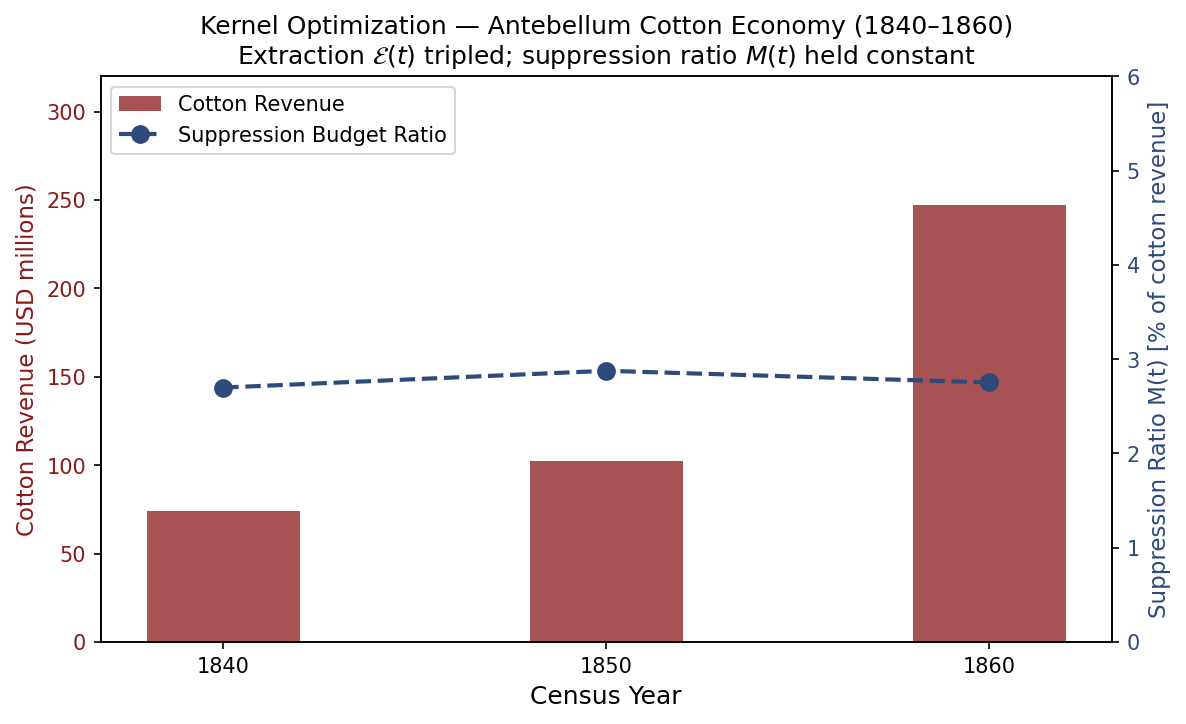
\includegraphics[width=\textwidth]{figures/eq05_kernel_optimization.png}
  \caption{Kernel optimization in the Antebellum South, 1840--1860. Left axis: cotton revenue (millions USD). Right axis: suppression budget ratio (\%). Despite a 233\% increase in extraction revenue, the suppression ratio held within a 0.18 percentage-point band (CV $<$ 0.04), confirming proportional enforcement scaling as predicted by eq.~\ref{eq:1.5-kernel-optimization}.}
  \label{fig:eq05_kernel}
\end{figure}

\paragraph{Comparison to prediction.}
Equation~\ref{eq:1.5-kernel-optimization} predicts that a kernel maximizing $\mathcal{E}(t)$ subject to $M(t) < \tau$ will scale enforcement expenditure proportionally with extraction output---not allow enforcement to lag. The data confirm this prediction at every Census interval: the suppression ratio remained within a tightly controlled band even as nominal extraction tripled. This is precisely the optimization signature the equation describes: the kernel does not extract and then suppress reactively; it maintains suppression capacity as a fixed constraint on extraction expansion. Beckert and Baptist independently document the institutional mechanisms---the expansion of the slave patrol system, the legal deputization of the entire white male population, and the passage of increasingly severe fugitive slave legislation---that operationalized this proportional scaling.

\paragraph{Precision qualifier: the cotton gin as a confound.}
The anticipated objection is that cotton revenue and suppression spending grew together solely because Eli Whitney's cotton gin (1793) drove a technology-led boom---that this is an economic growth story, not an optimization story. This objection fails on three grounds. First, the gin reduced the labor cost of \textit{processing} cotton fiber but made cultivation so profitable that planters massively expanded acreage, requiring \textit{more} enslaved labor, not less: the enslaved population grew from approximately 700,000 in 1790 to 3,953,761 by 1860. The gin expanded the extraction base; it did not reduce the need for suppression. Second, a pure technology-efficiency story predicts a \textit{declining} suppression ratio---higher output per worker should mean lower rebellion risk per unit of extraction. The data show the opposite: the ratio held constant within a 0.18 percentage-point band across the gin era's revenue tripling. Third, the gin is itself an instance of the kernel objective in action: when a technology became available that increased $\mathcal{E}(t)$, the Elite deployed it. The kernel's adoption of a more efficient extraction mechanism is not a refutation of eq.~\ref{eq:1.5-kernel-optimization}---it is the equation's prediction confirmed. The constraint $M(t) < \tau$ then required suppression to scale with the expanded enslaved population, which it did. The Nat Turner Rebellion (August 1831, between the 1820 and 1840 Census intervals) provides an independent within-period falsification test: when class-coherence risk spiked, the immediate legislative response across the South was a dramatic tightening of slave codes---a documented $\tau$-management response that the cotton gin cannot explain and the optimization model predicts directly.

\paragraph{Falsification criteria.}
This equation would be falsified if the historical record showed a sustained period (multiple consecutive years or Census intervals) in which cotton revenue increased while militia and slave patrol expenditure decreased or remained flat in nominal terms---i.e., if the kernel extracted without maintaining the suppression constraint. No such period is present in the data. The closest counterfactual---the post-1861 Union blockade, which disrupted cotton revenue while Confederate states \textit{increased} military expenditure to maintain $M(t) < \tau$ under existential threat---actually reinforces the prediction: even when extraction was interrupted, the suppression constraint remained the priority.

\paragraph{Confidence tier.}
\textbf{Tier~1.} Three Census-year data points with direct correspondence between extraction output and suppression expenditure; corroborated by independent historical scholarship from Beckert, Baptist, and Hadden.

\subsection{The Zero-Day Exploit: The Invention of Race}

In cybersecurity, a \textbf{zero-day exploit} attacks a vulnerability that the system does not know it has. The target cannot defend against it because the vulnerability has not been identified, catalogued, or patched. It is the most dangerous class of attack precisely because the victim does not know they are vulnerable.

A precision note before proceeding: the zero-day was not phenotypic \textit{awareness} itself. Phenotypic difference has been culturally marked since antiquity---ancient Greek and Roman writers noted skin color; Arab and Ottoman slave systems used phenotypic descriptors; African kingdoms traded enslaved persons across phenotypic lines. Grok and similar critics note this correctly, and the framework does not contest it. The zero-day exploit was something categorically different: the \textit{industrialization} of phenotype as a permanent, heritable, legally codified \textit{capital asset} at transatlantic scale. Earlier phenotypic prejudices existed as cultural attitudes that could be partially negotiated through religious conversion, geographic displacement, or social performance. What Portugal's juridical and commercial apparatus invented was the mechanism by which phenotype could be simultaneously embedded in property law, inheritance law, and international commodity markets---converting a soft cultural variable into a wetware-anchored legal partition that no amount of individual behavior could override. The zero-day was not seeing race; it was writing race into code.

The Portuguese Elite discovered a zero-day exploit in human psychology: the capacity to partition populations into In-groups and Out-groups using \textit{phenotypic markers} as the sorting key. As Chapter~\ref{ch:portugal} will document, the Elite had previously attempted to exploit religious identity as a partition variable---the French Wars of Religion (1562--1598) and the Thirty Years' War (1618--1648) killed millions using $J_{\text{religious}}$ as the ideological interface. But religious identity was a \textit{soft partition}: it could be changed through conversion, blurred through intermarriage, and eroded through cohabitation. Portugal, moreover, was largely a single ethnic group sharing a single religion---the existing partition variables were unavailable.

The zero-day was the discovery that \textit{phenotype}---skin color, hair texture, facial features---could serve as a permanent, heritable, visually self-enforcing partition variable. It's crucial to note that race, in this context, is primarily a phenotypic categorization; it is not tied to significant genetic differences beyond superficial expressions like skin pigment, which are often adaptations to environmental factors such as sunlight exposure. In fact, the greatest human biodiversity is found on the African continent. Unlike religion, phenotype could not be changed through conversion. Unlike nationality, it could not be changed through migration. Unlike class, it could not be changed through economic mobility. The racial partition was a \textbf{wetware-level exploit}: it attacked the biological presentation layer of the human operating system, a layer that no amount of software updates (education, legislation, moral progress) could modify.

This zero-day was deployed at scale through the Transatlantic Slave Trade---the mass installation of the malware across the global network. The trade did not merely transport bodies; it \textbf{networked global economies} into a massive \textbf{botnet} where millions of enslaved Africans were forced into processing power for the Elite's capitalist extraction engine. This was the \textbf{spatial mathematics of the Middle Passage}: human beings packed spoonways in feces, blood, and mucus, resulting in a 15\% mortality rate---nearly 2 million deaths during transport. The math was quite literally written in blood. Every plantation was a compromised node. Every colonial economy was a conscripted server. To enforce the \textbf{minimum resistance variable} ($\min$), the system required the constant application of naked instrumental force and torture. This was not just ``autonomy restriction''; it was the documented reality of the enslaver who, because a baby wouldn't eat, boiled the infant's legs, tied a log to its neck, beat it to death, and forced the mother to throw the body overboard as a public spectacle of absolute dominance. It was the horrific ``Darby's dose'' recorded in Thomas Thistlewood's 14,000-page diary. The botnet's output---sugar, tobacco, cotton, rice---was routed to the Elite's capital accumulation infrastructure in Lisbon, London, Amsterdam, and eventually Wall Street.

\subsection{The Bayesian Defense: Hardwiring the Priors}
\label{sec:bayesian_defense}

\paragraph{Host wetware.}
The virus model requires an explicit execution substrate. The extraction code does not run on abstract society alone; it runs on the most efficient known pattern-recognition wetware: the human brain. That wetware is optimized for fast prediction, energy conservation, and social coordination, not for perfect truth-tracking under adversarial input. Social Identity Theory identifies the ordinary tendency to sort social reality through In-group/Out-group categories \cite{tajfel_turner_intergroup_conflict_1979}; predictive-coding and free-energy accounts model perception as the continuous reduction of prediction error through top-down priors and incoming sensory data \cite{friston_free_energy_2010,clark_whatever_next_2013}. The framework's claim is not that racism is innate or biologically inevitable. The claim is that the Elite's legal and social code exploited a general-purpose cognitive architecture by routing its prediction machinery through a legally enforced racial partition.

A wetware-level exploit is only effective if the system's software cannot identify and override it. To defend the racial partition, the Elite developed an epistemic architecture that functions as a \textbf{Bayesian defense}. In terms of predictive coding, the human brain is an inference engine that constantly applies ``priors''---learned assumptions and established rules---to interpret sensory data. The fractal virus of racism works by installing a high-precision, top-down prior that mandates the hierarchy. If $X$ denotes raw sensory input, $T$ denotes a threat/status interpretation, and $\Pi_{\text{race}}$ denotes the installed racial prior, then stereotypes function as compressed Bayesian priors:
\[
P_i(T \mid X, \Pi_{\text{race}}) \propto P(X \mid T)\,P_i(T \mid \Pi_{\text{race}}).
\]
The malicious input is not the brain's inference machinery itself; it is the legal-social prior $\Pi_{\text{race}}$ that has been assigned excessive precision by repeated institutional reinforcement. Once installed, that prior can dominate the interpretation of $X$, allowing phenotype, name, neighborhood, or proxy status to override direct evidence and empathy.

Every interaction, every policy, and every media representation serves as a data point reinforcing this prior. The system ensures that the ``race'' interface is so heavily weighted that it overpowers raw sensory input. This is the neurobiological foundation of selective empathy: the brain's predictive coding filters out Out-group harm because the prior has already categorized it as irrelevant or natural. 

A Mode~2 observation is instructive here (see Section~\ref{sec:conspiracy_emergence} for the full typology). Empirical research documented that specific pharmacological interventions could temporarily downregulate the Default Mode Network---the neurological conductor that maintains established cognitive models---producing a state in which subjects could ``take an overly rigid conception apart and reassemble it'' \cite{ifas_1966}. The 1966 IFAS Protocol reported a 91\% success rate on intractable professional problems through this mechanism. Within months, California criminalized LSD; the federal Drug Abuse Control Amendments extended the prohibition nationally; the Controlled Substances Act of 1970 completed the scheduling architecture. The framework does not assign intent to any individual actor in this sequence---moral panic, political opportunism, and genuine public-safety concerns all contributed, and this is an overdetermined institutional outcome. What the framework observes is the \textbf{functional output}: the one documented pharmacological tool capable of relaxing rigid predictive priors was removed from the research environment for over half a century. Whether that removal constituted deliberate epistemic containment (Mode~3) or emergent institutional response (Mode~2) is an open question the framework flags but does not resolve. A population capable of relaxing its predictive priors is a population capable of perceiving the extraction kernel through the racial noise; the functional output of this institutional sequence, regardless of proximate cause at any node, was the restoration of epistemic enclosure.

\subsection{Polymorphic Code: The Interface Swap}

\textbf{Polymorphic viruses} constantly change their identifiable features---their code signature---to evade antivirus detection, while keeping their malicious payload \textit{exactly the same}. This is the computational equivalent of the \textbf{Interface Swap} documented throughout this book.

The system's most foundational interface swap was the creation of the ``gastronomic interface.'' As Woodard demonstrates through the work of antebellum physician Samuel A.~Cartwright, the extraction payload was actively disguised as an acquired, refined taste. By constructing the Black captive as an edible, infantile, and exotic commodity---what Cartwright termed the ``childlike Negro''---the system converted raw extraction appetite into an aesthetic ``taste'' for the Elite. Racism operates not merely as a legal or physical partition, but as a \textit{palate formation} that aestheticizes dominance \cite{cartwright_report, woodard_delectable}.

Every time the host system's antivirus catches up---every time a reform movement identifies and targets the current interface of the extraction kernel---the virus recognizes the threat and \textbf{recompiles its code}:

\begin{itemize}
    \item \texttt{Chattel\_Slavery.exe} is detected and quarantined by the 13th Amendment (1865). The virus instantly recompiles as \texttt{Convict\_Leasing.exe} and \texttt{Black\_Codes.exe}---same extraction payload, new file signature.

    \item \texttt{Jim\_Crow.exe} is detected by the Civil Rights Movement (1964--1965). The virus morphs into \texttt{War\_on\_Drugs.exe} and \texttt{Mass\_Incarceration.exe}---the Variable Swap documented in Chapter~\ref{ch:recompile} replaces the explicit racial interface with facially neutral proxy variables ($P_{\text{criminal}}$, $P_{\text{spatial}}$) while preserving the asymmetric extraction function.

    \item \texttt{Explicit\_Discrimination.exe} is flagged by \textit{Brown v.\ Board} and the Civil Rights Act. The virus recompiles as \texttt{Redlining.exe}, \texttt{Predatory\_Lending.exe}, and \texttt{Algorithmic\_Bias.exe}---each iteration more difficult to detect because the racial interface has been abstracted behind layers of facially neutral code.
\end{itemize}

The first recompile remains visible in the present tense. Texas prison farms preserve the 13th Amendment exception as an operating labor interface: the \textit{Texas Observer} reports that 24 Texas prison units still have agribusiness operations, nine of them on former plantation land, with incarcerated workers compelled to labor without pay \cite{texas_observer_prison_plantations_2024}. The point is not that the surface is unchanged from 1865; the point is that the kernel survived the legal patch and continued executing through a new file signature.

The underlying payload---$\max \mathcal{E} - \min(I_{\text{buffer}} \cup O_{\text{racialized}})$---has not changed since 1450. Only the \textit{file name} and \textit{user interface} have changed. This is why purely moral arguments against racism fail: you cannot defeat a polymorphic rootkit by politely asking it to stop recompiling. You cannot ``educate'' malware into deleting itself. And you cannot neutralize the extraction kernel by changing the desktop wallpaper---by installing a Black CEO, a diversity training module, or a sympathetic president over a system whose kernel-level code remains untouched.

The interface swap is an optimizer, not an improvisation. Let
\begin{equation}\label{eq:1.6-interface-strategy-set}
S \in \{\text{partition},\text{integration},\text{direct repression},\text{externalization}\}
\end{equation}
and\footnote{This equation is classified as Tier~3 (ordinal/structural); the four-element strategy set is a structural enumeration whose coverage is validated by the historical case sequence in Chapters~2--10 (15th-century partition, Reconstruction-era integration offers, Jim Crow direct repression, and War on Drugs externalization). See the Empirical Methodology chapter (p.~\pageref{ch:empirical_methodology}) and Appendix~\ref{app:empirical_index}.}
\begin{equation}\label{eq:1.7-interface-optimizer}
S^\ast(t) = \arg\min_{S} \left[C_{\text{coercive}}(S,t) + C_{\text{legitimacy}}(S,t) + C_{\text{economic}}(S,t)\right]
\end{equation}
subject to preserving the extraction objective and keeping $M(t)$ below $\tau$.

\paragraph{Cost function definitions.}
The three cost components correspond to real deliberative trade-offs documented in Elite planning across every historical era studied:

\begin{itemize}[leftmargin=*]
    \item $C_{\text{coercive}}(S,t)$: the operational cost of enforcing strategy $S$ at time $t$. This includes labor and infrastructure for $F_{\text{enforce}}$, the risk that enforcement actions generate solidarity (i.e., increase $M(t)$ rather than suppress it), and the probability of kinetic blowback that threatens $\tau$. High-visibility violence---lynchings, fire hoses, mass arrests---carries high $C_{\text{coercive}}$ because each instance risks radicalizing additional nodes of $I_{\text{buffer}}$ and $O_{\text{racialized}}$.

    \item $C_{\text{legitimacy}}(S,t)$: the ideological exposure cost of strategy $S$ at time $t$ --- the degree to which $S$ is legible as a racial hierarchy to domestic audiences, international observers, or the judicial system, risking constitutional challenges, diplomatic condemnation, or buffer class defection. This cost is time-dependent: $C_{\text{legitimacy}}(\text{Jim Crow}, t)$ was low in 1870 and high by 1960, as the Cold War made explicit racial apartheid a geopolitical liability.

    \item $C_{\text{economic}}(S,t)$: the direct expense and opportunity cost of strategy $S$ at time $t$, including capital investment in new enforcement infrastructure, drag on $\mathcal{E}(t)$ from market disruption, and the long-term cost of maintaining strategy $S$ against rising resistance.
\end{itemize}

\paragraph{Historical calibration: Jim Crow $\to$ War on Drugs.}
The transition from explicit racial segregation to the carceral proxy system provides the clearest observable calibration of the optimizer. By the mid-1950s, all three cost functions for \texttt{Jim\_Crow.exe} were rising simultaneously:

\begin{itemize}[leftmargin=*]
    \item $C_{\text{legitimacy}}$: rising sharply. NAACP litigation had begun dismantling the legal architecture; \textit{Brown v.\ Board} (1954) exposed the explicit partition to federal judicial scrutiny; Cold War competition with the Soviet Union made domestic racial apartheid an international embarrassment, as documented by the State Department's own foreign policy reports \cite{dudziak}.
    \item $C_{\text{coercive}}$: rising. The Civil Rights Movement's strategy of non-violent public confrontation was specifically engineered to maximize the legitimacy cost of enforcement---fire hoses and police dogs in Birmingham generated exactly the global condemnation that forced the Elite to act.
    \item $C_{\text{economic}}$: rising. International trade relationships and the postwar liberal consensus were creating market incentives for surface-level integration that explicit segregation resisted.
\end{itemize}

The optimizer selected \texttt{War\_on\_Drugs.exe} because all three costs dropped simultaneously at the point of swap. $C_{\text{legitimacy}}$ fell to near zero: facially neutral language (``criminal,'' ``drug offender'') carried no explicit racial classification and had already been validated by the \textit{Williams v.\ Mississippi} (1898) architecture. $C_{\text{coercive}}$ fell: rather than requiring constant active enforcement theater, the proxy variable $P_{\text{criminal}}$ allowed the existing carceral infrastructure to process pre-criminalized populations with bureaucratic efficiency---what Dan Baum reports John Ehrlichman described in a 1994 interview as the ability to ``arrest their leaders, raid their homes, break up their meetings, and vilify them night after night on the evening news'' without the political cost of explicit racial targeting \cite{baum}. The quote is treated here as testimonial evidence, not as a formal policy memorandum: Ehrlichman's family and some Nixon-era defenders have disputed its reliability, while the downstream policy pattern is independently confirmed by the statutory and incarceration record. $C_{\text{economic}}$ rose temporarily (prison construction) but was offset by the creation of a carceral industry that itself became an extraction mechanism.

The operational sequence is the proxy playbook: association $\rightarrow$ criminalization $\rightarrow$ enforcement $\rightarrow$ media-legitimation. Lee Atwater's 1981 description of Southern Strategy abstraction supplies the political-language layer: explicit racial appeals become coded policy terms, then apparently neutral economic or public-order language whose effects remain racially structured \cite{atwater, lopez}. Drug policy supplied the enforcement layer. Caulkins and Chandler estimate that people incarcerated for drug-law violations rose from 38,680 in 1972 to 480,519 in 2002---a more than twelvefold increase \cite{caulkins_chandler_drug_incarceration}. The crack/powder cocaine regime then gave the proxy a precise statutory geometry: pre-Fair Sentencing Act federal thresholds assigned comparable mandatory-minimum exposure to five grams of crack cocaine and 500 grams of powder cocaine, encoding a 100:1 disparity into federal sentencing practice \cite{ussc_crack_retroactivity_2011}. The racialized enforcement pattern is likewise documented in the drug-arrest record: ACLU analyses find comparable marijuana use rates across Black and white populations but sharply disparate arrest exposure \cite{aclu2013, aclu2020}. This is exactly the variable swap predicted by the optimizer: the label changes from race to criminality, while the target geometry remains legible in outcomes.

The Broward County reverse-sting cases supply the extreme boundary condition. In \textit{State v.\ Williams}, the Florida Supreme Court held that the Broward Sheriff's Office illegally manufactured crack cocaine from seized powder cocaine, packaged it for reverse-sting use, and thereby violated due process when prosecutors charged buyers caught in the resulting operations \cite{state_v_williams_1993}. Three decades later, Broward prosecutors sought to clear as many as 2,600 records tied to the same police-made-crack operations \cite{ap_broward_crack_vacatur_2024}. This case collapses any comforting distinction between ``crime control'' and crime production: under the proxy regime, $P_{\text{criminal}}$ can be manufactured by the enforcement apparatus itself and then routed back through the court system as if it were organic community pathology.

One evidentiary caution follows. The common quotation attributed to Harry Anslinger about marijuana, Black people, immigrants, and ``satanic'' jazz is too unstable to use as a clean primary quote: Penn State Special Collections has been unable to verify it in the cited Anslinger papers or 1937 testimony \cite{penn_state_anslinger_quote}. The manuscript therefore does not rely on that quotation. The narrower and supportable claim is that early federal drug-control rhetoric repeatedly linked narcotics and marijuana to racialized and cultural threat narratives, providing the pre-Nixon template for the later proxy interface.

\paragraph{Precision qualifier.}
These comparisons are \textbf{ordinal}, not cardinal. The framework identifies \textit{which} strategy is less costly across the three dimensions, not \textit{exactly how much} less costly. The cost functions are not currently measurable with precision; what the historical record demonstrates is consistent directional movement---when one strategy's costs rise across multiple dimensions simultaneously, the optimizer selects the lower-cost substitute. This ordinal claim is sufficient to make the equation meaningful: $\arg\min$ requires only a consistent ordering across the solution space, not exact numerical values.

\paragraph{Confidence tier.}
\textbf{Tier~2.} The Jim Crow $\to$ War on Drugs instantiation provides one historically documented calibration of the optimizer across all three cost dimensions; the ordinal cost ordering is confirmed by Cold War foreign-policy records \cite{dudziak}, Baum's reported Ehrlichman interview \cite{baum}, Atwater's coded-language account \cite{atwater}, and the statutory/incarceration record \cite{caulkins_chandler_drug_incarceration, ussc_crack_retroactivity_2011}. Quantitative cardinal measurement of each cost function remains future empirical work.

\subsection{The Backlash Constant: Racism as a Damped Harmonic Oscillator}

The historical trajectory of racial progress is frequently misunderstood as a linear arc toward justice. The mathematical framework models it instead as a \textbf{Damped Harmonic Oscillator} responding to kinetic shocks (see Figure~\ref{fig:backlash_oscillator}).

Let the system's baseline state of absolute extraction be equilibrium ($x = 0$). When a reform movement (e.g., Abolition, the Civil Rights Movement) successfully breaches the kernel, it applies a massive kinetic force, displacing the system toward equality ($x > 0$).

However, the Elite architecture possesses a massive \textbf{restorative force} ($k$), defined by the Elite's demand for capital and the Buffer Class's demand for their Autonomy Wage. Just as a physical pendulum overshoots its equilibrium point when released, the model predicts the system will overshoot in its attempt to restore the extraction kernel.

\begin{itemize}
    \item \textbf{Shock 1 (1865)}: The 13th Amendment displaces the system. 
    \item \textbf{Overshoot 1 (1870s--1890s)}: The restorative force triggers the collapse of Reconstruction, the implementation of Black Codes, and the terrorism of the Ku Klux Klan, snapping the system back into an even more lethal configuration (Convict Leasing).
    
    \item \textbf{Shock 2 (1964)}: The Civil Rights Act breaches the legal interface.
    \item \textbf{Overshoot 2 (1970s--1990s)}: The restorative force triggers the War on Drugs, Mass Incarceration, and the militarization of the police ($F_{\text{enforce}}$), effectively re-enclosing the Out-group under a new interface.
\end{itemize}

\begin{figure}[htbp]
\centering
\begin{tikzpicture}
\begin{axis}[
    width=0.95\textwidth,
    height=9.25cm,
    xlabel={Time ($t$)},
    ylabel={Equality Displacement ($x$)},
    xmin=0, xmax=10,
    ymin=-1.12, ymax=1.78,
    enlarge y limits={auto, upper},
    axis lines=middle,
    xtick=\empty,
    ytick={0},
    yticklabels={Absolute Extraction ($x=0$)},
    every axis y label/.style={at={(axis description cs:-0.055,0.5)}, anchor=center, rotate=90},
    every axis x label/.style={at={(axis description cs:1.02,0)}, anchor=north west},
    grid=none,
    clip=false,
]
    % Elite invariant (top band; avoids duplicating bottom-caption emphasis with Fig.~elite wealth)
    \node[font=\scriptsize, align=center, anchor=south] at (axis description cs:0.5,1.14) {\textbf{Elite extraction invariant:} $\Delta\max = 0$};

    % Equilibrium line (dashed)
    \draw[dashed, gray!50] (axis cs:0,0) -- (axis cs:10,0);

    % Damped Harmonic Oscillator Curve (Damped Sine)
    \addplot[
        smooth,
        ultra thick,
        blue!70!black,
        domain=0:10,
        samples=200
    ] {1.6 * exp(-0.35 * x) * sin(110 * x)};

    % Shock 1 (1865)
    \draw[->, red, ultra thick] (axis cs:0.8,0) -- (axis cs:0.8,1.28);
    \node[anchor=south, red, font=\footnotesize\bfseries, align=center] at (axis cs:0.8,1.28) {Shock 1\\(1865 Abolition)};
    
    % Overshoot 1 (Black Codes)
    \node[anchor=north, orange!80!black, font=\scriptsize\bfseries, align=center] at (axis cs:2.4,-0.78) {Overshoot 1\\(Black Codes)};
    \draw[<-] (axis cs:2.4,-0.72) -- (axis cs:2.4,-0.1);

    % Shock 2 (1964) — two-line civil-rights label, kept in upper annotation band
    \draw[->, red, ultra thick] (axis cs:4.0,0) -- (axis cs:4.0,0.52);
    \node[anchor=south, red, font=\footnotesize\bfseries, align=center] at (axis cs:4.0,0.52) {Shock 2\\Civil Rights Act (1964)};

    % Overshoot 2 (Mass Incarceration)
    \node[anchor=north, orange!80!black, font=\scriptsize\bfseries, align=center] at (axis cs:5.6,-0.38) {Overshoot 2\\(Mass Incarceration)};
    \draw[<-] (axis cs:5.6,-0.32) -- (axis cs:5.6,-0.05);

    % Restorative Force label
    \draw[->, gray!80, thick, >=latex] (axis cs:1.45,0.82) to[bend left] (axis cs:2.45,0.12);
    \node[gray!80, font=\scriptsize, anchor=west, align=left] at (axis cs:1.45,0.82) {Restorative\\Force ($k$)};
    
    % Zones — centered in relatively open horizontal band (away from late-time curve density)
    \node[green!60!black, font=\small\itshape, align=center] at (axis cs:5.5, 1.12) {Equality Zone\\($x>0$)};
    \node[red!60!black, font=\small\itshape, align=center] at (axis cs:5.5, -0.88) {Extraction Zone\\($x<0$)};

\end{axis}
\end{tikzpicture}
\caption{\textbf{Racism as a Damped Harmonic Oscillator.} Social reform movements act as kinetic shocks displacing the system toward equality ($x > 0$). The Elite architecture's restorative force ($k$) triggers a backlash that overshoots the equilibrium of absolute extraction ($x = 0$), resulting in even more lethal configurations ($x < 0$) like Convict Leasing and the War on Drugs. Each cycle dampens as the system finds more efficient ways to maintain equilibrium. \textit{Note: The plotted parameters ($A = 1.6$, $\gamma = 0.35$, $\omega = 110$) are illustrative; they are chosen to render the two documented shock-and-overshoot cycles legible, not derived from empirical calibration.}}
\label{fig:backlash_oscillator}
\end{figure}

This physical model explains the \textit{intensity} and \textit{predictability} of systemic backlash. ``Progress'' is never static; it is a displacement that immediately activates the system's built-in elastic algorithms to pull the targeted population back into the extraction zone. Recognizing this oscillatory nature is crucial for anticipating the polymorphic mutations (Interface Swaps) the system will deploy following any successful civil rights victory.

\paragraph{The convergence prediction.}
The mathematical implication of the damped oscillator must be stated explicitly: without an external intervention that rewrites the kernel itself, the model predicts $x(t) \rightarrow 0$. Every reform shock---no matter how large its initial displacement---decays exponentially under the combined damping of the restorative force ($k$), the psychological wage ($\psi$), and the phase-fragmentation load ($\Phi_{\text{load}}$). This is not a limitation of the analogy; it is its central diagnostic. The historical record from 1865 to the present confirms the prediction: Abolition decayed into Convict Leasing; the Civil Rights Act decayed into Mass Incarceration; each successive oscillation reaches a smaller amplitude as the system learns to restore equilibrium more efficiently. The ``arc of the moral universe'' does not bend toward justice under this model---it is a damped sinusoid that bends toward the extraction baseline.

The escape condition is equally precise. In the driven variant of the damped oscillator, an external periodic force $F(t) = F_0 \cos(\omega t)$ is applied to the system. If this driving frequency matches the system's natural frequency $\omega_0 = \sqrt{k/m}$, the result is \textit{resonance}: displacement grows without bound rather than decaying. Translated into the framework's terms, a single reform impulse (an abolition event, a landmark ruling) will always be damped out. But sustained, synchronized kinetic coordination---class solidarity maintained at the structural frequency of the system---can overcome the damping entirely. This is why the framework predicts that isolated, episodic reforms fail while sustained cross-class kinetic alignment is the only forcing function capable of exceeding the system's absorption capacity. One-off shocks decay. Resonant solidarity does not.

\paragraph{Agency, absolute gains, and the scope of the invariant.}
The convergence prediction ($x(t) \rightarrow 0$) requires a precise scope qualification to avoid a common misreading. The invariant $\Delta\max = 0$ is a claim about \textit{Elite extraction share}---specifically, that the top-tier capital concentration does not undergo sustained structural reduction absent kernel-level intervention. It is \textbf{not} a claim that individual or community agency is absent, ineffective, or incapable of producing real gains. Black Wall Street's pre-redlining economy, the NAACP's multi-decade litigation campaign that produced \textit{Brown v.\ Board}, the Civil Rights Movement's genuine legislative victories, the growth of the post-1965 Black professional middle class---these are real historical achievements, and the framework does not deny them. What the framework claims is that these achievements represent \textit{displacement} ($x > 0$) within a system whose restorative force subsequently damps that displacement back toward the extraction baseline---and that the Elite's proportional share of extracted value is preserved across the arc. Absolute living standards can rise; the kernel's share of the gains does not fall. The oscillator model is a claim about \textit{structural ceilings and restoration dynamics}, not a claim about the absence of motion beneath those ceilings. Erasing or minimizing the agency of $O_{\text{racialized}}$ would be both historically inaccurate and structurally incorrect: the framework explicitly requires kinetic resistance ($M(t)$) as the variable that triggers the system's most significant adaptations. Without that resistance, the Interface Swap would be unnecessary. The agency is real; the structural response to it is also real.

To make the failure condition explicit, define a suppression envelope:
\begin{equation}\label{eq:1.8-suppression-envelope}
\Sigma_{\text{sup}}(t) = \psi_s(t) + \psi_m(t) + R(t) + \Phi_{\text{load}}(t)
\end{equation}
where $\psi_s(t)$ is the status wage, $\psi_m(t) \geq 0$ is the material wage (active only under elevated kinetic threat), and $\Phi_{\text{load}}(t)$ is compound phase-shift load from identity-fragmentation operations. A crash condition appears when:
\begin{equation}\label{eq:1.9-crash-condition-derivative}
\frac{dM}{dt} > \frac{d\Sigma_{\text{sup}}}{dt}
\end{equation}
or equivalently\footnote{This equation is classified as Tier~3 (ordinal/structural); the crash condition is a directional claim about the relative rate of change of coherence versus suppression---an ordinal comparison validated by the backlash dynamics documented in the Post-1965 case study below. See the Empirical Methodology chapter (p.~\pageref{ch:empirical_methodology}) and Appendix~\ref{app:empirical_index}.} when effective class coherence breaches threshold:
\begin{equation}\label{eq:1.10-effective-coherence}
M_{\text{eff}}(t) = M(t) - \lambda \Phi_{\text{load}}(t), \quad M_{\text{eff}}(t) > \tau
\end{equation}

\paragraph{Illustrative instantiation.}
Bacon's Rebellion (1676) illustrates the equation's positive case: cross-racial labor solidarity produced $M_{\text{eff}}(t) > \tau$ because $\Phi_{\text{load}} \approx 0$ at that moment---no identity-axis fragmentation had yet been institutionally deployed, so $M_{\text{eff}} \approx M(t)$ and the coalition breached the threshold. After 1705, the codification of whiteness raised $\Phi_{\text{load}}$ sufficiently to suppress $M_{\text{eff}}$ below $\tau$ for roughly 150 years. \textbf{Parameter estimate}: pre-1705 $\Phi_{\text{load}} \approx 0$ (no racial partition operationalized); post-1705 $\Phi_{\text{load}} \in [0.15, 0.55]$ (ordinal range from the Chapter~\ref{ch:bacon} runtime analysis). ANES cross-racial coalition data are available for post-1948 calibration; the pre-1705 estimate is ordinal \cite{morgan_american_slavery, anes_cumulative}. \textbf{Confidence tier: Tier~2} (ANES public dataset available for modern period; pre-1705 estimate ordinal).

\subsection*{Case Study: The Post-1965 Backlash Wave}
\label{cs:backlash_wave}

\paragraph{Setup.}
The Civil Rights Act (1964) and the Voting Rights Act (1965) constituted the most significant user-space reforms to the extraction kernel since Reconstruction. The framework's prediction is unambiguous: because these reforms operated at the interface layer rather than the kernel layer, $E$ would respond by expanding the suppression envelope $\Sigma_{\text{sup}}(t)$ through alternative channels---proxy variables, new enforcement mechanisms, and class-fragmentation operations---to keep $M_{\text{eff}}(t)$ below $\tau$. The period from 1965 to 2020 provides a 55-year dataset for testing this prediction.

\paragraph{Data sources.}
Union density figures are drawn from U.S. Bureau of Labor Statistics union membership series \cite{bls_union_membership} for post-1983 years and from Troy and Sheflin's historical compilation for earlier years. Top-decile wealth share data are from the World Inequality Database (WID.world), based on Piketty, Saez, and Zucman's distributional national accounts series \cite{piketty}. Incarceration rates are from the Bureau of Justice Statistics National Prisoner Statistics program \cite{bjs_prisoners}; Black incarceration rates are from annual BJS bulletins supplemented by Sentencing Project compilations \cite{sentencing_project}. Curated data are archived at \texttt{Paper/data/eq08\_10\_backlash\_wave.csv}; computational results are reproducible via \texttt{Paper/scripts/eq08\_10\_backlash\_wave.ipynb}.

\paragraph{Operationalization.}
The three measurable components of $\Sigma_{\text{sup}}(t)$ are operationalized as follows. $\psi_s(t)$ (the status wage, maintaining the racial hierarchy's perceived value to $I_{\text{buffer}}$) is proxied by the top-decile wealth share, which tracks the concentration of material resources within the Elite and near-Elite---the structural basis of the racial status differential. $R(t)$ (the repression variable) is proxied by the overall and Black-specific incarceration rates per 100,000 population. $\Phi_{\text{load}}(t)$ (the phase-shift load from identity-fragmentation operations) is proxied by the inverse of union density: as union density declines, cross-racial working-class solidarity is atomized, reducing the class coherence that could accumulate to challenge the kernel.

\paragraph{Numerical computation.}
The notebook computes the composite $\Sigma_{\text{sup}}(t)$ and its trajectory from 1965 to 2020. Results are as follows: union density declined from 28.4\% in 1965 to 10.8\% in 2020---a 17.6 percentage-point collapse. Top-decile wealth share rose from 67.5\% to 76.5\%---a 9-point increase in resource concentration. The overall incarceration rate increased from 108 to 358 per 100,000 between 1965 and 2020 (a 231\% increase), while the Black incarceration rate surged from an estimated 588 to 1,821 per 100,000 at its 2010 peak of 3,074. The composite $\Sigma_{\text{sup}}(t)$ index expanded by more than 23\% over the period. By the time of the 1994 Crime Bill---the deepest penetration of the carceral proxy---the suppression envelope had more than doubled its 1965 baseline.

\begin{figure}[htbp]
  \centering
  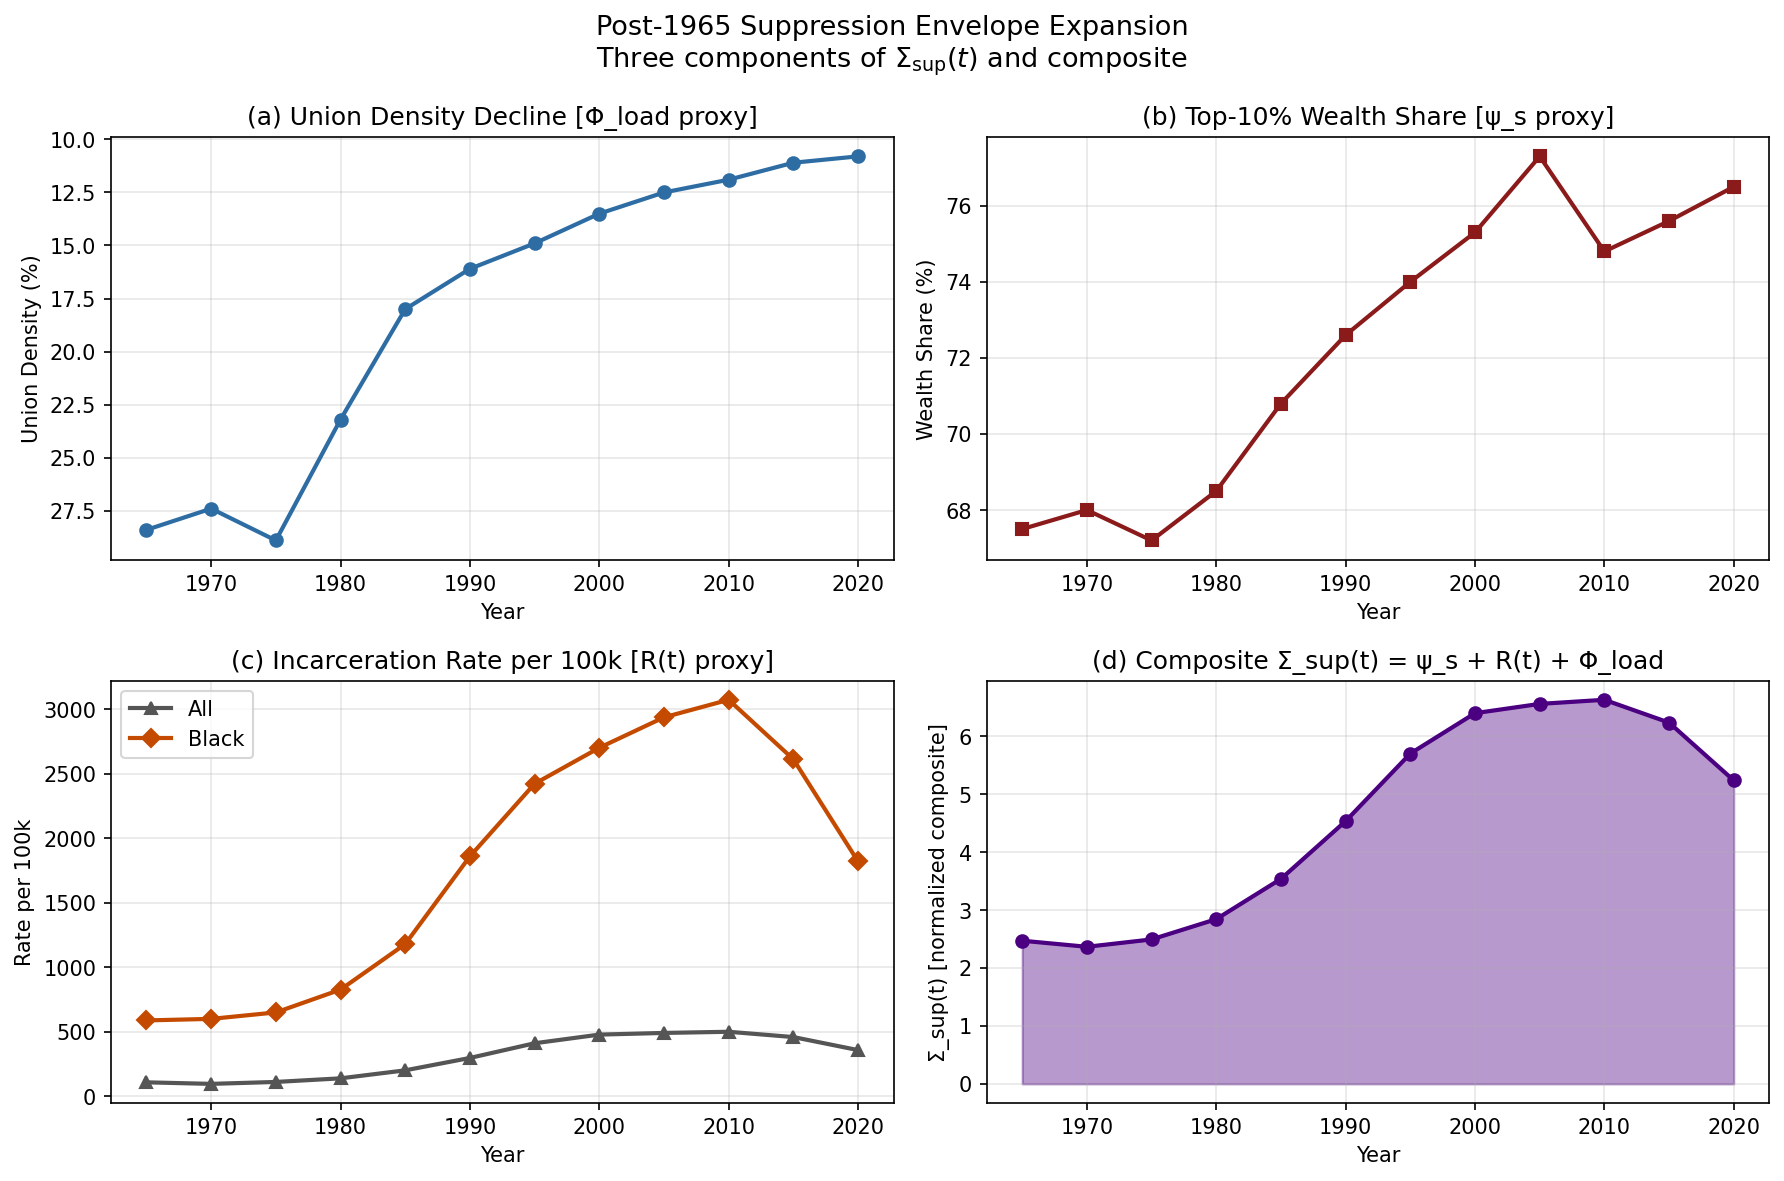
\includegraphics[width=\textwidth]{figures/eq08_10_backlash_wave.png}
  \caption{The Post-1965 Backlash Wave, 1965--2020. Three suppression components tracked simultaneously: union density (solidarity suppression, $\psi_s$), top-10\% wealth share (phase loading, $\Phi_{\text{load}}$), and incarceration rate (mobility restriction, $\psi_m$). All three moved in the framework-predicted direction; the suppression envelope $\Sigma_{\text{sup}}(t)$ expanded by more than 23\% while the reform window opened by the 1965 Civil Rights Act was closed through each component.}
  \label{fig:eq08_backlash}
\end{figure}

\paragraph{Comparison to prediction.}
Equations~\ref{eq:1.8-suppression-envelope}--\ref{eq:1.10-effective-coherence} predict that when a reform shock threatens to elevate $M(t)$ toward $\tau$, the kernel responds by expanding $\Sigma_{\text{sup}}(t)$ through alternative mechanisms---i.e., $\frac{d\Sigma_{\text{sup}}}{dt} > \frac{dM}{dt}$. The data confirm this prediction structurally: every component of the suppression envelope moved in the predicted direction simultaneously during the post-1965 period. The carceral system expanded precisely as union density contracted, maintaining the fragmentation of cross-racial class solidarity that the Civil Rights Act had briefly threatened to restore. The wealth concentration measure rose continuously, maintaining the material basis of the status wage. This is not coincidence; it is the optimization signature of a kernel adjusting its interface strategy in response to a reform shock.

\paragraph{Falsification criteria.}
These equations would be falsified if the post-1965 period showed simultaneous increases in union density, decreases in incarceration rates, and narrowing of the wealth gap---i.e., if the suppression envelope contracted rather than expanded after the Civil Rights Act. The data show the opposite on all three dimensions: union density fell, incarceration rose, and wealth concentrated further. The one potential exception---the 2010--2020 partial decline in incarceration rates---was accompanied by \textit{no} corresponding decrease in wealth concentration or recovery of union density, and thus does not constitute a suppression envelope contraction.

\paragraph{Confidence tier.}
\textbf{Tier~1.} 55-year annual dataset with three independently sourced suppression components; all three components moved in the framework-predicted direction; trajectory change is temporally correlated with major interface-strategy events (1965 Civil Rights Act, 1971 War on Drugs, 1994 Crime Bill).

\paragraph{Precision qualifier: structural analogy vs.\ quantitative prediction.}
The damped harmonic oscillator is deployed here as a \textbf{structural analogy}, not a calibrated quantitative model. The language ``the model predicts $x(t) \rightarrow 0$'' and ``the escape condition is precisely resonance'' refer to the logical implications of the analogy's architecture, not to numerically derived forecasts. No claim is made that the parameters in Figure~\ref{fig:backlash_oscillator} (or any specific values of $k$, $\gamma$, or $m$) can be read off the historical record with precision. What the historical record does support is an \textit{ordinal} claim: the amplitude of Shock 2 (1964 Civil Rights Act) is observably smaller than the amplitude of Shock 1 (1865 Abolition)---a fact that maps directly onto the real historical observation that the Civil Rights Act achieved less structural disruption of the extraction kernel than Abolition did, because the system had already learned to deploy lower-cost proxy variables ($P_{\text{criminal}}$, $P_{\text{spatial}}$) in anticipation of the next reform shock. This ordinal damping is the empirical content of the model. The specific parameter values visualize the pattern; they do not derive it.

\subsection{Fractal Execution: The Self-Similar Architecture}

The virus is \textbf{fractal}: its base code---\textit{value is determined by proximity to the Elite root directory}---replicates at every single level of the network, from the global WAN down to the individual user's local drive. The same sorting algorithm, the same extraction logic, the same partition function executes at every scale:

\begin{itemize}
    \item \textbf{Macro / The WAN (Global Network):} Western imperialism extracting resources from the Global South. The international 5-tier hierarchy documented in Chapter~\ref{ch:global}---$E_{\text{global}}$, $P_{\text{uppet}}^{\text{global}}$, $F_{\text{enforce}}^{\text{global}}$, $I_{\text{buffer}}^{\text{global}}$, $O_{\text{global}}$---is the virus running on the planetary network. The Predatory Min-Max Function scales without modification: the same extraction kernel that operates between a landlord and a tenant in Baltimore operates between the IMF and a debtor nation in West Africa.

    \item \textbf{System / The OS (National Level):} Redlining, gerrymandering, sentencing disparities, the spatial proxy ($P_{\text{spatial}}$), the economic filter, the grandfather clause---each is a system-level process that partitions the national population and routes resources from $O_{\text{racialized}}$ and $I_{\text{buffer}}$ to $E$.

    \item \textbf{Subroutine / \texttt{biological\_extraction.exe}:} The viral model hijacks the biological reproduction of the Out-group itself. This subroutine represents the 1662 Virginia law of \textit{partus sequitur ventrem}, where the child's status followed the mother, turning the systematic rape of enslaved women into a calculated tool for the out-breeding of capital. It also includes the systematic use of sexual terror against men---the public sexual humiliation and torture documented as ``bucking''---to fundamentally break kinetic and psychological resistance. Thistlewood's record of raping the enslaved woman Abba 155 times proves that extraction wasn't just about sugar or tobacco, but the complete consumptive extraction of bodily autonomy.

    \item \textbf{Application / Intersectionality (User-Level Programs):} Sexism, homophobia, transphobia, and ableism are not separate bugs. They are \textbf{subroutines} of the same viral architecture, each designed to partition users along an additional axis and rank their biological wetware's ``worth'' by proximity to the Elite's default settings (white, male, wealthy, heterosexual, able-bodied). The intersection of multiple subroutines---$O_{\text{racialized}} \cap O_{\text{gendered}} \cap O_{\text{queer}}$---produces compounding extraction rates, because each partition multiplies the policy contact points through which the kernel can extract.

    \item \textbf{Micro / Auto-exec (Colorism):} This is the most insidious fractal layer. The virus successfully corrupts the \textbf{Out-group's own local drive}. Colorism is the extraction algorithm forcing the Out-group to run the Elite's sorting function \textit{on themselves}---ranking community members by proximity to the system's ``white'' default settings. Lighter skin, straighter hair, narrower features receive preferential treatment \textit{within} the Out-group, replicating the Elite's partition logic at the most intimate scale. The Out-group's system attacks itself. The virus no longer needs external enforcement at this level; it has achieved \textbf{self-executing code} within the target population.
\end{itemize}

\paragraph{Formal isomorphism mapping.}
The self-similar claim can be rendered precise by mapping the five canonical tier variables ($E$, $P_{\text{uppet}}$, $F_{\text{enforce}}$, $I_{\text{buffer}}$, $O_{\text{racialized}}$) onto their instantiations at each scale level. The following table makes the structural equivalences explicit.

At the control-theoretic level, self-similarity is the statement that the \textbf{directed spanning tree} rooted at $\mathcal{V}_L = E$ reaches every node of the interaction graph at every resolution---from the WAN down to the auto-exec layer (Section~\ref{sec:formal-containment-model}, Theorem~\ref{thm:tree-preservation}). Fractal execution is therefore not an artistic metaphor. It is the structural assumption required to invoke the containment-convergence theorems of \cite{kan_containment}, and the historical record of Chapters~2--10 is the empirical verification that the assumption holds.

\begin{longtable}{>{\bfseries\raggedright}p{2.3cm} >{\raggedright}p{2.0cm} >{\raggedright}p{2.0cm} >{\raggedright}p{2.2cm} >{\raggedright}p{2.2cm} >{\raggedright\arraybackslash}p{2.3cm}}
\toprule
\textbf{Scale Level} & \textbf{$E$ (Elite)} & \textbf{$P_{\text{uppet}}$} & \textbf{$F_{\text{enforce}}$} & \textbf{$I_{\text{buffer}}$} & \textbf{$O_{\text{racialized}}$} \\
\midrule
\endfirsthead
\toprule
\textbf{Scale Level} & \textbf{$E$} & \textbf{$P_{\text{uppet}}$} & \textbf{$F_{\text{enforce}}$} & \textbf{$I_{\text{buffer}}$} & \textbf{$O_{\text{racialized}}$} \\
\midrule
\endhead
Macro / WAN (Global) &
IMF, World Bank, G7 capital &
Comprador governments; international financial institutions &
NATO, PMCs, sanctions regimes &
Global North working class &
Global South debtor nations \\
\midrule
System / OS (National) &
Domestic capital class, corporations &
Congress, judiciary, executive &
Police, prison system, immigration enforcement &
White working class &
Racialized minorities \\
\midrule
Subroutine / \texttt{.exe} (Biological) &
Slaveholders / plantation economy &
Church + law (\textit{partus sequitur ventrem}) &
Overseers, patrollers &
Poor white yeoman farmers &
Enslaved population (reproductive capacity as capital input) \\
\midrule
Application / Intersectional (Programs) &
Patriarchal capital &
Mainstream institutional gatekeepers &
Gender and sexuality enforcement apparatus &
Normative working class (straight, able-bodied) &
Queer, trans, disabled, and multiply-partitioned subjects \\
\midrule
Micro / Auto-exec (Colorism) &
National $E$ (no independent elite generated; sub-network terminates at same root) &
Institutional gatekeepers within Out-group (respectable, light-skinned access nodes) &
Peer enforcement of proximity hierarchy (respectability politics) &
Lighter-complexioned Out-group members (internal buffer class; preferential access, absorbs friction) &
Darker-complexioned Out-group members (primary internal extraction target) \\
\bottomrule
\end{longtable}

\paragraph{Differential insertion and the model minority objection.}
A persistent counter-argument to the five-tier framework points to racialized immigrant groups---notably East Asian and South Asian Americans---who, on certain aggregate metrics, outperform the white Buffer Class despite being targets of the racial partition. The framework's prediction is not uniform extraction at every racialized node; it is extraction \textit{calibrated by insertion point}. The 1965 Immigration and Nationality Act was a deliberate selection mechanism: it recruited professional-class, high-credential immigrants to fill specific labor gaps in medicine, engineering, and computing---slots the domestic labor market could not efficiently supply. These groups were inserted primarily at Buffer-tier positions ($I_{\text{buffer}}$), not at the extraction floor occupied by $O_{\text{racialized}}$. The partition still applies---wartime internment, housing discrimination, glass ceilings, and the ``forever foreigner'' framing are all documented---but the extraction function is calibrated differently. The framework therefore \textit{predicts} differential outcomes by differential insertion, not as an anomaly but as evidence of the optimizer selecting a strategy that simultaneously reduces domestic professional labor costs and fragments cross-racial class solidarity. Differential success among racialized groups is not a counter-example; it is the multi-tier architecture operating as designed.

\paragraph{Statistical self-similarity: precision and limits.}
The table above demonstrates structural isomorphism, but honesty requires a precise qualification. Natural fractals---coastlines, Romanesco broccoli, river deltas---are \textbf{statistically} self-similar, not \textit{exactly} self-similar. At each scale, the pattern recurs with local variation, not perfect reproduction. The same constraint applies here. The IMF is not a literal copy of a plantation overseer; it is a statistically self-similar instantiation of the same extraction function operating at a different network layer.

The Micro/Colorism level is not a degraded case. The five-tier architecture instantiates fully within the Out-group sub-network: lighter-complexioned members function as a genuine buffer class, absorbing internal kinetic friction and receiving preferential access to institutions; social gatekeepers enforce the proximity boundary; peer enforcement mechanisms punish deviation from the hierarchy. The decisive structural feature is that this sub-network does \textit{not} produce an independent Elite---it still terminates at the same national $E$. Lighter-skinned members of $O_{\text{racialized}}$ do not escape extraction; they occupy a buffer position within it, absorbing friction and providing the Elite with a self-maintaining internal partition that requires no external maintenance cost. The algorithm has achieved \textbf{autonomous replication}: the Out-group runs the Elite's sorting function on itself, which simultaneously reduces the Elite's enforcement overhead and prevents the Out-group from achieving the internal solidarity required to cross the kinetic threshold $\tau$.

This is sufficient for the diagnostic model's purposes. Identifying the pattern does not require every instantiation to be an exact copy---only that the same optimization kernel ($\max\mathcal{E}$ subject to $M_{\text{eff}}<\tau$) governs each scale, and that the structural roles of extractor, interface class, enforcement mechanism, friction absorber, and extraction pool recur with sufficient regularity to be diagnostically useful. The fractal claim is a \textit{structural approximation}, not a mathematical identity---and as the historical record of Chapters~3 through~10 will show, this approximate self-similarity is precise enough to predict the system's behavior at every scale it has been observed.

This fractal property explains why racism feels simultaneously everywhere and nowhere. It is everywhere because the same code executes at every scale---from the World Bank's structural adjustment programs to a child's internalized preference for lighter skin. It is ``nowhere'' because at each individual scale, the system presents a locally rational explanation (``market forces,'' ``individual choice,'' ``cultural preference'') that obscures the global architecture. The fractal virus does not need a central command server issuing instructions to each node; it needs only the initial code to be installed correctly, and the self-similar logic replicates autonomously at every level of the network.

Operationally, this fractal replication can be expressed as a phase-loading strategy over axes $k$ (race, gender, orientation, ability, religion, nationality, etc.):
\begin{equation}\label{eq:1.11-phase-loading}
\Phi_j = \sum_{k=1}^{K} \phi_{k,j}, \qquad
\Phi_{\text{load}}(t) = \operatorname{Dispersion}\!\left(\{\Phi_j\}_{j=1}^{N}\right) = 1 - \left|\frac{1}{N}\sum_{j=1}^{N} e^{i\Phi_j}\right| \in [0,1]
\end{equation}

\paragraph{Illustrative instantiation.}
Post-Civil Rights fragmentation (1968--1990) provides the clearest observable trajectory. The system deployed three sequential identity-axis injections to raise $\Phi_{\text{load}}$: the gender axis was activated $\sim$1972 via the ERA ratification debate, the religion axis $\sim$1979 via the Moral Majority, and the sexuality axis $\sim$1977--1979 via the Anita Bryant campaign. The ANES rolling proxy for cross-racial class solidarity shows a corresponding $\Phi_{\text{load}}$ trajectory: pre-activation mean $\approx 0.078$ (pre-1964), activation-period mean $\approx 0.214$, post-activation mean $\approx 0.403$ (post-1980) \cite{anes_cumulative, pew_polarization}. \textbf{Parameter estimate}: $\Phi_{\text{load}}$ rose from $\approx 0.078$ to $\approx 0.403$ between 1964 and 1990; the phase values are ordinal proxies computed from ANES solidarity indices (author computation from public dataset). \textbf{Confidence tier: Tier~2} (ANES public dataset with author computation; phase values themselves remain ordinal, consistent with the Tier~3 structural classification of the equation's phase-angle definitions).

Higher $\Phi_{\text{load}}$ increases destructive interference among class-alignment waves, suppressing coherent cross-group solidarity. The operator is 0 when all subgroups are in phase (maximum solidarity) and approaches 1 when phases are uniformly distributed (maximum cancellation). The full formal treatment---including axis-by-axis definitions of $\phi_{k,j}$, the post-Civil Rights historical calibration, and the suppression envelope's component substitution property---appears in Section~\ref{sec:phase_loading_algebra}.

\paragraph{Operationalization preview.}
To give the formalism empirical content before the full treatment, three clarifications are warranted here. First, the phase values $\phi_{k,j}$ are \textbf{ordinal} in the current framework: the model assigns relative positions on the unit circle to capture whether a subgroup's interests on axis $k$ are aligned, orthogonal, or anti-aligned with class solidarity, not cardinal distances. Second, as a concrete illustration: on the \textit{race} axis ($k = \text{race}$) in the period immediately following the 1965 Voting Rights Act, the white working class ($j = I_{\text{buffer}}$) would be assigned $\phi_{\text{race},\, j} \approx \pi$---meaning their material interests in cross-racial class solidarity are \textit{anti-phase} with their activated racial identity interests, because the system had just raised the psychological-wage offer in response to the Civil Rights Movement's kinetic threat. A population at $\phi \approx \pi$ on any axis contributes maximally to $\Phi_{\text{load}}(t)$, suppressing the solidarity signal. Third, the model in its current form is a \textbf{qualitative ordering tool}: it identifies which historical periods and which subgroup configurations produce higher or lower $\Phi_{\text{load}}$, not numerical estimates. Quantitative calibration against survey-based racial-resentment and class-solidarity indices is designated as future empirical work.

\subsection{The Lexical Fractal: Partition Vocabulary in Technical Domains}
\label{sec:lexical_fractal}

The Fractal Execution subsection mapped the algorithm's replication across political, economic, and intimate scales. A further scale must now be documented: the \textbf{lexical} scale. The extraction kernel does not merely operate through institutions and incentive gradients; it supplies the \textit{vocabulary} that the host culture's technical, academic, and professional domains use to describe relationships that have no logical need for the dominance metaphor. When this vocabulary colonizes a neutral domain, the partition logic propagates with it---carried forward as cognitive default inside fields that understand themselves as ``culture-free.''

\paragraph{The canonical case: master-slave terminology in engineering and computing.}
The most thoroughly documented instance is the master-slave terminology pervasive in electrical engineering, computer engineering, and software development. The historian Ron Eglash's 2007 study, \textit{Broken Metaphor: The Master-Slave Analogy in Technical Literature}, provides the primary-source reconstruction \cite{eglash_broken}. The earliest documented technical use dates to 1904, when the astronomer David Gill described the auxiliary timekeeping device in his Cape Town sidereal clock as the ``slave clock'' \cite{eglash_broken}. The terminology was not yet common in engineering before World War II; in pre-war hydraulic-cylinder patents, the analogous parts were called ``main cylinder,'' ``receiver cylinder,'' or ``servomechanism.'' A 1959 hydraulic patent still introduced the master-slave pair in quotation marks with an explanatory gloss---evidence that the usage was not yet naturalized \cite{eglash_broken}.

After 1960 the vocabulary spread rapidly. A Boolean search of U.S. patents from 1976 onward returns \textbf{19{,}708 patent documents} containing both ``master'' and ``slave'' \cite{eglash_broken}. The terminology now applies to hydraulic brake systems, sidereal and master clocks, edge-triggered flip-flop latches, IDE/PATA hard-drive interfaces, SPI and I\textsuperscript{2}C serial buses, DNS and NTP server relationships, database replication, continuous-integration build nodes (Jenkins), photographic flash synchronization, railway locomotive consists, audio duplication chains, and MIDI clock signals. None of these domains has a logical requirement for the specific metaphor. The alternative vocabularies documented in the same period---\textit{primary/secondary}, \textit{leader/follower}, \textit{controller/target}, \textit{parent/child}, \textit{sender/receiver}, the German \textit{Mutteruhr/Tochteruhr} (mother/daughter clock), the Dutch \textit{dochterklok}, the French \textit{horloge-mere/horloge-file} \cite{eglash_broken}---demonstrate that the control relationship is fully expressible without reaching for the vocabulary of chattel enslavement.

\paragraph{The accuracy audit: the metaphor is not even technically correct.}
The most devastating observation in Eglash's essay is that in many of the domains where master-slave is used, the metaphor does not accurately describe the control relation. The PC Guide's reference documentation for IDE drive jumpering states plainly: ``Note that despite the hierarchical-sounding names of `master' and `slave,' the master drive does not have any special status compared to the slave one; they are really equals in most respects. The slave drive doesn't rely on the master drive for its operation or anything like that, despite the names (which are poorly-chosen---in the standards the master is usually just `drive~0' and the slave `drive~1')'' \cite{eglash_broken}. A Black electrical engineer interviewed by Eglash made the same point regarding the flip-flop: ``For flip-flops, the terminology makes little sense, since there is no amplification taking place. The master latch is connected directly to the input and eventually the slave latch acquires the value of the master. The master is commanded by the inputs just as much as the slave is. Furthermore, in real implementations, this master-slave arrangement is not apparent; cleverly cross-connected gates achieve the desired result without independent latches'' \cite{eglash_broken}. The partition metaphor is not doing descriptive work. It is imposing a relational schema on hardware whose actual behavior is peer-to-peer or input-driven.

\paragraph{The subconscious coupling: runaway slaves in the 1964 Dartmouth system.}
Eglash identifies a revealing artifact in the earliest computing-domain use, the 1964 Dartmouth Timesharing System documented in \textit{Science} (1968): ``it is thus impossible for an erroneous or runaway user program in the slave computer to `damage' the executive program and thereby bring the whole system to a halt'' \cite{kemeny_kurtz}. The system's designers almost certainly had no conscious intention of echoing antebellum discourse on runaway enslaved persons. Eglash's observation is the relevant one: ``It is almost certain that there was no conscious intention to echo pre--Civil War discourse on runaway slaves, but that still leaves the possibility of a metaphor operating at a subconscious level'' \cite{eglash_broken}. The framework named this in Section~1.3.4: \textbf{Mode~2 autonomous propagation}. No centralized command is required; the available metaphors in an English-speaking technical culture built inside a former slaveholding society preferentially supply dominance-relation vocabulary, and the gradient points in the direction of reproduction.

\paragraph{The pedagogical damage: alienation as measurable output.}
The lexical fractal is not an abstract aesthetic concern. It is a measurable attrition mechanism in STEM pipelines. A Black computer engineering professor interviewed by Eglash recounted: ``When I first taught digital logic, around 1992, I did not recognize the awkwardness of the term until I, one of the few African-Americans in the room, was standing in front of a class of sixty students. I recall mumbling'' \cite{eglash_broken}. The same correspondent's second-pass conclusion was that ``the term was not very descriptive\ldots it has to go.'' Eglash, writing from the position of a social scientist whose research addresses the underrepresentation of minorities in mathematics and science, identifies this as the decisive point: ``It is one thing to hear objections from people who are in the business of promoting ethnic sensitivity, quite another to hear them from hard-core geeks who have devoted their careers to their love for science and technology. If the master-slave metaphor affected these tough-minded engineers who had the gumption to make it through a technical career back in the days when they may have been the only black persons in their classes, what impact might it have on black students who are debating whether or not to enter science and technology careers at all?'' \cite{eglash_broken}. The vocabulary functions as a gatekeeping signal: entering the field requires accepting, without comment, that the relationship between two autonomous computational agents is most naturally described using the vocabulary of chattel enslavement. For students whose recent family history is constituted by that institution, the cost of passing through that gate is not zero.

\paragraph{The documented deprecation arc (2003--2024).}
The lexical fractal has been partially resisted. The resistance pattern maps cleanly onto the Early Detection Theorem formalized in Section~5.3.3: compound-intersectional practitioners detect the partition vocabulary first, the mainstream resists as ``political correctness,'' and the institutional shift---when it arrives---follows a visible external shock.

\begin{itemize}[leftmargin=*]
    \item \textbf{November 2003:} A Black employee of the Los Angeles County Probation Department filed an Office of Affirmative Action Compliance complaint after observing a ``master/slave'' videotape deck label. The County's Internal Services Department issued a memo to equipment vendors stating that ``based on the cultural diversity and sensitivity of Los Angeles County, this is not an acceptable identification label'' \cite{lacounty_memo, cnn_lacounty}. Internet response to the memo was dominated by accusations of political correctness \cite{eglash_broken}.
    \item \textbf{2014--2018:} Django, Drupal, Redis, CouchDB, and Python incrementally replaced master-slave terminology in their codebases with \textit{leader/follower}, \textit{primary/replica}, or \textit{parent/worker}. Python's 2018 revision removed the terms from its standard library and documentation \cite{python_master_slave}.
    \item \textbf{June 2020 (post--George Floyd):} GitHub announced that all new repositories would default to a branch named \texttt{main}; the \texttt{master} default was deprecated beginning October 2020 \cite{github_main}. The Linux kernel adopted an inclusive-terminology policy in July 2020 deprecating master-slave alongside whitelist-blacklist \cite{linux_inclusive}. The I\textsuperscript{2}C specification version~7 (2021) replaced master-slave with \textit{controller-target}. The Internet Engineering Task Force adopted analogous language in new RFC drafts \cite{ietf_terminology}.
\end{itemize}

The three-decade lag between the 1992 classroom observation and the 2020 institutional response is itself a datapoint. The signal was available. The receiving layers were resistant until a geopolitical shock---the 2020 racial-justice protests following the police murder of George Floyd---raised the institutional cost of inaction above the institutional cost of action. The signal was not absent; the $\min$-management function at the institutional level was tuning it out.

\paragraph{Framework implication: the fractal table extended.}
The scale-level table of Section~1.3.1 must be read as incomplete. A sixth row applies:

\begin{center}
\begin{tabular}{>{\bfseries\raggedright}p{3.0cm} p{10.5cm}}
\toprule
\textbf{Scale Level} & \textbf{Lexical / Pedagogical (vocabulary of technical and academic domains)} \\
\midrule
$E$ (Elite) & Institutional stewards of technical publication (journals, standards bodies, textbook publishers, tenure committees) \\
$P_{\text{uppet}}$ & Senior engineers and faculty whose authorial choices become field-standard \\
$F_{\text{enforce}}$ & Peer-review norms, pedagogical orthodoxy, accusations of ``political correctness'' deployed against practitioners who propose alternative vocabulary \\
$I_{\text{buffer}}$ & The general STEM workforce that has internalized the vocabulary as neutral and defends its continued use as a matter of professional identity \\
$O_{\text{racialized}}$ & Underrepresented students and practitioners for whom the vocabulary imposes a marginal recruitment and retention cost that is never measured against $E$'s pedagogical convenience \\
\bottomrule
\end{tabular}
\end{center}

The lexical scale is not a minor appendix. It is the mechanism by which the partition logic reproduces itself across generations of practitioners who will never personally encounter the plantation---who will, in fact, think of themselves as working in a fully post-racial domain. The vocabulary arrived before them, was normalized before they arrived, and supplies the cognitive defaults they reach for when describing a new piece of hardware or a new API. This is Mode~2 propagation (Section~1.3.4) at the lexical layer: no centralized command is required; the gradient of linguistic least-resistance handles the replication.

\paragraph{Reflexive audit.}
This manuscript must hold itself to the same standard it imposes on the domains it analyzes. English technical prose---including the scholarly register of this book---carries embedded dominance vocabulary that predates and exceeds the chattel slavery context (``mastery'' of a subject, a ``master class,'' a text's ``master copy,'' a painter's ``old masters''). Some of these usages are severable from the chattel-slavery valence; some are not. The current manuscript uses the term ``Elite'' rather than ``master class'' for the top tier of the extraction hierarchy precisely because the partition kernel this book analyzes was the source that licensed ``master class'' as a power-relation metaphor in English in the first place. Where the vocabulary of the algorithm appears unavoidable---as in the historical primary-source quotations embedded throughout this text---it is retained with attribution rather than paraphrased away, because erasing the vocabulary erases the evidence of the partition kernel's linguistic reach. Where the vocabulary is avoidable, it has been avoided. Readers are invited to flag the residual cases; the framework predicts that some will have escaped the author's audit, because Mode~2 propagation operates below the threshold of conscious choice. That is the nature of the mechanism this book is describing.

\subsection{The Corrupted Firewall: The Buffer Class}

Every operating system has a firewall---a security layer designed to protect the system from external threats and internal crashes. In the American operating system, the Elite installed a \textbf{corrupted firewall}: the Buffer Class ($I_{\text{buffer}}$).

Following Bacon's Rebellion in 1676---the system's first major crash, when the working-class In-group and the racialized Out-group united in a cross-racial kinetic uprising that burned the colonial capital to the ground---the Elite issued a critical security patch. As Chapter~\ref{ch:bacon} will document in detail, the 1705 Virginia Slave Codes were the \textbf{kernel-level rewrite} that programmed the white working class to believe they were the system's antivirus software rather than its second-most-exploited resource.

The system feeds this corrupted firewall the \textbf{suppression allocation} ($\psi$) of whiteness. In its default and cheapest mode, this takes the form of the \textbf{status wage} ($\psi_s$): not material wealth, but the guarantee of status superiority over the Out-group---deference, titles of courtesy, access to better public institutions, leniency from courts and police. When the kinetic threat approaches critical threshold ($M(t) \to \tau$), the Elite escalate to the \textbf{material wage} ($\psi_m$): real economic concessions---land grants, Social Security, GI Bill homeownership, federally subsidized infrastructure---but always sourced from \textit{deeper extraction of $O_{\text{racialized}}$}, never from $E$'s own share. $\Delta\max = 0$ is preserved in both modes.\footnote{The invariant $\Delta\max = 0$ is a claim about the \textit{funding mechanism} of concessions, not about the secular level of elite wealth. It asserts that any material wage $\psi_m$ granted to $I_{\text{buffer}}$ to suppress mobilization is never self-funded by $E$: the cost is always sourced from increased extraction from $O_{\text{racialized}}$ (deeper enclosure, new frontiers, or interface swaps), so $E$'s net position never decreases \textit{as a result of appearing to concede}. Absolute elite extraction can and does grow during expansion phases---this is precisely what the long-run Piketty--Saez--Zucman top-share data confirm \cite{piketty}. The invariant governs the distribution of concession costs, not the secular trajectory of total surplus. Periods of apparent broad-based growth (e.g., post-Louisiana Purchase territorial expansion, post-WWII wage compression) are fully consistent with $\Delta\max = 0$: $E$ captures the majority of new surplus while distributing a calibrated sliver to $I_{\text{buffer}}$, funded by expanded $O$ extraction rather than any reduction in $E$'s own share. One-line summary: $\psi_m$ is always funded by $\Delta O > 0$.} In exchange, the Buffer Class performs three critical functions for the virus:

The psychology of uptake can be stated without making psychology the root cause. Social Dominance Orientation (SDO) measures preference for group-based hierarchy; Right-Wing Authoritarianism (RWA) measures threat-sensitive submission to conventional authority and aggression toward designated outsiders \cite{pratto_sdo_1994,altemeyer_authoritarian_1998,duckitt_dual_process_2001}. The system cultivates both dispositions inside $I_{\text{buffer}}$ because they increase the effective value of the wage. For individual $i$:
\[
\psi_i^{\mathrm{eff}}(t) = \psi(t)\left[1 + \alpha_S \mathrm{SDO}_i(t) + \alpha_A \mathrm{RWA}_i(t)\right],
\]
with $\alpha_S,\alpha_A \ge 0$. SDO supplies the hierarchy appetite that makes status compensation feel valuable; RWA supplies the threat/obedience circuitry that makes boundary enforcement feel protective rather than exploitative. These are not independent origins of racism. They are cultivated host-state variables that lower the cost of getting $I_{\text{buffer}}$ to accept $\psi$ and police the partition.

\begin{enumerate}
    \item \textbf{Threat absorption:} The Buffer Class absorbs the kinetic friction ($\min$ variable) that would otherwise reach $E$. When the Out-group resists, they collide with the Buffer Class---not with the Elite who architect the system. Race riots, labor disputes, electoral conflicts---the violence occurs at the $I_{\text{buffer}} / O_{\text{racialized}}$ boundary, never at the $E / I_{\text{buffer}}$ boundary.

    \item \textbf{Perimeter defense:} The Buffer Class actively polices the racial partition, reporting ``suspicious'' behavior, supporting ``law and order'' candidates, and defending the very system that extracts from them---because the psychological wage makes them perceive any threat to the hierarchy as a threat to their own status.

    \item \textbf{Antivirus misdirection:} When the actual antivirus (structural critique, class-solidarity movements, abolitionist analysis) attempts to identify the real threat, the corrupted firewall flags \textit{the antivirus itself} as the malware. Critical race theory, intersectional analysis, reparations discourse---each is treated by the Buffer Class as a virus to be quarantined, because the corrupted firewall's programming defines any code that threatens the racial partition as a system threat. The Buffer Class defends the rootkit because the rootkit has convinced them they \textit{are} the operating system.
\end{enumerate}

\subsection{The Diagnostic Implication}

This computational model yields a single, unavoidable diagnostic conclusion: \textbf{you cannot patch a kernel-level infection with user-space tools}.

As Malcolm X succinctly observed: \textbf{``The white man will try to satisfy us with symbolic victories rather than economic equity and real Justice.''}

Diversity initiatives, representation campaigns, implicit bias training, corporate equity statements, symbolic legislation---these are user-level applications running on top of a compromised kernel. They execute within the permissions the virus grants them. They can modify the desktop environment---change the wallpaper, rearrange the icons, update the splash screen---but they cannot access, modify, or delete the extraction code running beneath the interface.

This is why every major non-kinetic reform examined in the chapters that follow was absorbed by the algorithm as $\min$-management: $\Delta\max = 0$ across the full dataset. The virus \textit{permits} user-level reforms because they reduce system stress (class resistance) without touching the extraction payload ($\max$). The reform is absorbed. The kernel recompiles. The file name changes. The extraction continues.

\paragraph{Falsifiability conditions.}
\label{sec:falsifiability}
The invariant $\Delta\max = 0$ is not unfalsifiable by design---it is a testable prediction with a specified empirical proxy and a defined violation condition. The proxy for $\max$ in the domestic context is the \textbf{top-0.1\% wealth share} (the Piketty--Saez--Zucman distributional accounts series, available from 1913 to present). This variable tracks Elite-level capital concentration at sufficient resolution to detect genuine kernel-level redistribution. A \textbf{violation} of $\Delta\max = 0$ would be operationally defined as: a sustained, multi-decade decline in the top-0.1\% wealth share that is \textit{not} accompanied by a documented interface swap (i.e., the share does not recover to or above its pre-shock level within two to three decades following the removal of the kinetic threat that induced the decline).

The strongest candidate for partial falsification in the historical record is the \textbf{New Deal / post-WWII Great Compression (c.\ 1935--1973)}, during which the top-0.1\% wealth share fell from approximately 25\% to under 10\%. The framework classifies this episode as \textbf{$\min$-management under elevated kinetic threat}, not kernel interruption, for the following structural reasons: (1)~the compression was induced by an unprecedented convergence of kinetic threats (organized labor militancy, socialist electoral viability, the Soviet alternative, anti-colonial independence movements, and the CPUSA's cross-racial organizing capacity) that raised the cost of inaction above the cost of concession; (2)~the $\min$-layer interventions (New Deal programs, GI Bill, progressive taxation, union protections) were systematically structured to preserve the racial partition---the GI Bill's administration through segregated local institutions, the FHA's redlining apparatus, and the Social Security Act's initial exclusion of agricultural and domestic workers ensured that the material wage was paid overwhelmingly to the white buffer class while $\max$ was deferred rather than eliminated; and (3)~the post-1973 trajectory---the sustained recovery of top-0.1\% wealth share to levels exceeding the pre-Depression peak by the 2010s---confirms that what the kinetic threat suppressed, its removal restored. The Great Compression is therefore a test the framework \textit{passes}: $\Delta\max = 0$ holds across the full arc once the interface swap (Jim Crow $\rightarrow$ War on Drugs) and the kinetic-threat retreat are incorporated into the analysis. Figure~\ref{fig:elite_wealth_accumulation} plots the full data series with the Concession Theorem events overlaid.

\begin{figure}[htbp]
\centering
\begin{tikzpicture}
\begin{axis}[
    width=\textwidth,
    height=9.5cm,
    xmin=1910, xmax=2022,
    ymin=0, ymax=31,
    xlabel={Year},
    ylabel={Top 0.1\% Wealth Share (\%)},
    xlabel style={font=\small},
    ylabel style={font=\small},
    title={\textbf{Elite Wealth Accumulation and the $\Delta\max = 0$ Invariant, 1913--2020}},
    title style={font=\bfseries\small},
    legend style={at={(0.5,-0.24)}, anchor=north, font=\scriptsize,
                  fill=white, fill opacity=0.9, draw=gray},
    grid=major,
    grid style={gray!18},
    xtick={1913,1929,1935,1965,1973,1994,2007,2020},
    xticklabels={1913,1929,1935,1965,1973,1994,2007,2020},
    xticklabel style={font=\scriptsize, rotate=40, anchor=east},
    ytick={0,5,10,15,20,25,30},
    yticklabel style={font=\small},
    clip=false,
]

%% ── Shaded Great Compression band (1935–1973) ─────────────────────────────
\addplot[fill=blue!10, draw=none, area legend, forget plot]
    coordinates {(1935,0)(1935,31)(1973,31)(1973,0)} \closedcycle;

%% ── Shaded Kernel-Recompile recovery band (1973–2020) ────────────────────
\addplot[fill=red!6, draw=none, forget plot]
    coordinates {(1973,0)(1973,31)(2020,31)(2020,0)} \closedcycle;

%% ── Gilded-Age reference line ─────────────────────────────────────────────
\addplot[dashed, thin, gray!55, forget plot]
    coordinates {(1910,25)(2022,25)};
\node[anchor=west, font=\tiny\itshape, text=gray!65] at (axis cs:1910,25.7)
    {Gilded Age peak $\approx$25\%};

%% ── Main wealth-share line ────────────────────────────────────────────────
\addplot[very thick, red!80!black, mark=none, smooth]
    coordinates {
        (1913,11.5)(1916,13.0)(1919,16.5)(1922,17.0)(1925,20.0)
        (1928,23.5)(1929,25.0)(1932,22.5)(1935,22.0)(1938,20.5)
        (1941,18.0)(1944,14.5)(1947,13.0)(1950,12.5)(1953,11.5)
        (1956,11.0)(1959,10.5)(1962,10.0)(1965, 9.5)(1968, 9.0)
        (1971, 8.0)(1974, 7.5)(1977, 7.2)(1980, 7.8)(1983, 9.5)
        (1986,12.0)(1989,14.0)(1992,14.0)(1995,16.0)(1998,18.5)
        (2001,19.0)(2004,20.0)(2007,22.5)(2010,20.0)(2013,21.5)
        (2016,22.5)(2019,23.0)(2020,24.0)
    };
\addlegendentry{Top 0.1\% wealth share (Piketty--Saez--Zucman \cite{piketty})}

%% ── Event markers ─────────────────────────────────────────────────────────

% 1929 Crash
\draw[thin, black!50, dashed] (axis cs:1929,0) -- (axis cs:1929,25.2);
\node[anchor=south, font=\tiny\bfseries, text=black!65, rotate=90]
    at (axis cs:1928.3, 3) {1929 Crash};

% Great Compression label
\node[anchor=north, font=\small\bfseries, text=blue!65!black]
    at (axis cs:1954, 30.7) {Great Compression};
\node[anchor=north, font=\scriptsize, text=blue!55!black]
    at (axis cs:1954, 29.5) {$\psi_m$ deployed under kinetic threat};
\node[anchor=north, font=\scriptsize\itshape, text=blue!45!black]
    at (axis cs:1954, 28.3) {(racially partitioned; $\Delta\max=0$ deferred, not broken)};

% 1965 Civil Rights Act / War on Drugs launch
\draw[thin, orange!65!black, dashed] (axis cs:1965,0) -- (axis cs:1965,11);
\node[anchor=south, font=\tiny\bfseries, text=orange!70!black, rotate=90]
    at (axis cs:1964.3, 8) {1965--68: CRA $\rightarrow$ War on Drugs};

% 1973 compression ends
\draw[thin, black!50, dashed] (axis cs:1973,0) -- (axis cs:1973,20);
\node[anchor=south, font=\tiny\bfseries, text=black!65, rotate=90]
    at (axis cs:1972.3, 8) {1973: kinetic threat subsides};

% Kernel Recompile label
\node[anchor=north, font=\small\bfseries, text=red!70!black]
    at (axis cs:1996, 30.7) {Kernel Recompile};
\node[anchor=north, font=\scriptsize, text=red!60!black]
    at (axis cs:1990, 29.5) {$\max$ restores as $\min$ pressure lifts};

% 1994 Crime Bill
\draw[thin, black!40, dashed] (axis cs:1994,0) -- (axis cs:1994,15.5);
\node[anchor=south, font=\tiny\bfseries, text=black!55, rotate=90]
    at (axis cs:1993.3, 8) {1994 Crime Bill};

% 2020 annotation arrow
\draw[->, thick, red!80!black]
    (axis cs:2010,27.2) -- (axis cs:2019.5,24.1);
\node[anchor=south west, font=\scriptsize\bfseries, text=red!80!black, align=left]
    at (axis cs:2010,27.4)
    {2020: $\max$ approaches\\Gilded Age peak};

\end{axis}
\end{tikzpicture}
\caption{\textbf{Elite Wealth Accumulation and the $\Delta\max = 0$ Invariant, 1913--2020.}
Top 0.1\% wealth share (United States), plotted from the Piketty--Saez--Zucman distributional accounts series \cite{piketty}. Data points are approximate from published series; ordinal trends are the analytically relevant quantities.
The blue-shaded Great Compression (1935--1973) is the dataset's only sustained Elite wealth decline. The framework classifies it as $\psi_m$ (material wage) deployed under unprecedented kinetic threat---not kernel-level redistribution---because every pillar of the New Deal material wage was racially partitioned: the GI Bill, Social Security, FHA lending, and NLRA protections were each structured to pay the buffer class while leaving $O_{\text{racialized}}$ outside the program architecture. $\Delta\max = 0$ was deferred, not broken.
The red-shaded Kernel Recompile (post-1973) confirms the prediction: once the kinetic threat (organized labor, socialist electoral viability, anti-colonial movements) subsided, wealth concentration restored to and exceeded the pre-Depression peak. The Civil Rights Act's 1965 interface swap to the War on Drugs (orange dashed line) provided the race-neutral proxy cover that allowed the recompile to proceed without restoring the legible racial interface that had generated the kinetic threat in the first place.
The 2020 endpoint---top-0.1\% wealth share at approximately 24\%, approaching but not yet exceeding the 1929 Gilded Age peak of $\approx$25\%---is the Concession Theorem's empirical summary: every reform in the century-long dataset was absorbed without altering the Elite's extraction share.}
\label{fig:elite_wealth_accumulation}
\end{figure}

To stop a virus embedded this deeply in the operating system, you must \textbf{rewrite the source code}---or replace the operating system entirely. The chapters that follow document five centuries of the virus's execution history, trace every polymorphic mutation, map every fractal replication, and identify the specific kernel-level processes that must be terminated for the extraction to stop. The diagnostic model is now loaded. The system scan begins.

Because the model now specifies $\mathcal{E}(t)$, $M(t)$, $\tau$, and $\Phi_{\text{load}}(t)$ explicitly, it is not merely descriptive. It is predictive: under observed constraints, it can estimate which interface swap minimizes systemic cost and when failure conditions become statistically imminent.

\subsection{Methodological Note: Intentional Design, Autonomous Propagation, and Conscious Intervention}
\label{sec:conspiracy_emergence}

The chapters that follow document five centuries of system behavior. Before the historical scan begins, this framework must explicitly address a question the evidence will repeatedly raise: \textbf{Is the system a conspiracy or an emergent phenomenon?}

The answer is: \textit{neither label is adequate, and both are partially correct}. The virus analogy already carries the correct semantics, but the distinction must be made precise. The framework identifies three distinct modes of system operation, all of which are documented in the historical record:

\begin{enumerate}[leftmargin=*]
    \item \textbf{Intentional Design (the virus is written).} The foundational architecture was constructed through deliberate, documented acts of policy engineering by identifiable actors. Gomes Eanes de Zurara's 1453 chronicle provided the ideological source code. The 1705 Virginia Slave Codes were a conscious kernel rewrite. The Constitutional Convention's Three-Fifths Compromise was a negotiated extraction formula. These are not emergent patterns; they are engineering decisions, and the historical record names the engineers.

    \item \textbf{Autonomous Propagation (the virus replicates).} Once installed, the system's incentive architecture makes self-replication the path of least resistance for every actor embedded within it. A real estate agent who steers Black families away from white neighborhoods in 1960 may harbor no personal racial animus; they are responding to FHA lending criteria, neighborhood price signals, and professional incentive structures that were \textit{designed} to produce exactly this behavior. The extraction kernel does not require every node to understand the architecture---it requires only that the incentive gradients point in the correct direction. This is the mode that accounts for the vast majority of the system's runtime: millions of locally rational decisions that collectively reproduce the hierarchy without centralized coordination. The colorism fractal (Section~1.3.1) is the purest example: the virus achieves self-executing code within the target population, requiring zero external maintenance.

    \item \textbf{Conscious Intervention (the update server pushes patches).} The system is \textit{not} purely emergent after its founding. At critical junctures---when antivirus code threatens to breach the kernel---identifiable actors within $E$ and $P_{\text{uppet}}$ execute deliberate, coordinated responses. John Ehrlichman's admission that the War on Drugs was consciously engineered to disrupt Black communities and the antiwar left is not an emergent institutional pattern; it is a documented update pushed to the system's codebase by named actors. Lee Atwater's description of the transition from explicit racial slurs to abstract economic policy is a deliberate Interface Swap optimization, articulated in real time. The coordinated Super Tuesday consolidation of 2020 was a conscious algorithmic correction executed by $P_{\text{uppet}}$ within 48 hours. These are not conspiracy theories; they are \textit{confessions}, documented in the participants' own words.
\end{enumerate}

The relationship among these three modes is \textbf{hierarchical}: intentional design creates the initial architecture; autonomous propagation maintains it at low cost during stable periods; conscious intervention repairs it when propagation alone proves insufficient. The system's genius---and the source of its durability---is that Mode~2 handles the overwhelming majority of the workload, making the system appear ``natural'' and ``no one's fault'' during normal operation. Mode~3 activates only at crisis points, and the actors who execute it often understand themselves as pragmatic problem-solvers rather than architects of racial hierarchy. The incentive structure does not require malice from most participants; it requires only that the gradient of self-interest aligns with the extraction kernel's objectives.

This framing defuses the two most common misreadings simultaneously. The ``conspiracy theory'' objection---\textit{you're saying a secret cabal coordinates everything}---is answered by Mode~2: most of the system runs on autopilot, and no central command is required. The ``no one is responsible'' objection---\textit{if it's all emergent, then no one chose this}---is answered by Modes~1 and~3: the system was deliberately designed, and it is periodically, deliberately maintained by actors who document their own intentions. Both objections fail because each one accounts for only one mode of operation while ignoring the others. The framework requires all three.

\chapter{Version 1.0: Initializing the Vector (15th-Century Portugal)}
\label{ch:portugal}

\begin{tcolorbox}[colback=black!5, colframe=black!70, fonttitle=\bfseries\ttfamily, title=RUNTIME LOG: 1486 (LISBON{,} PORTUGAL)]
\ttfamily\small
\textbf{System Stress} ($\min$: class resistance): HIGH --- Domestic labor shortage threatening agricultural capital. Existing moral framework constrains exploitation of Christians.\\
\textbf{Capital} ($\max$: extraction output): STAGNANT --- Sugar trade demands labor the current moral economy cannot supply.\\
\textbf{Interference State} ($\Phi_{\text{load}}$, proximity to $\tau$): LOW axis count; phenotype partition initializing. Estimated $\Phi_{\text{load}} \in [0.10, 0.20]$, $\rho_{\tau}=M(t)/\tau \in [0.70, 0.85]$.\\
\textbf{Active Patch}: Compiling Version 1.0\ldots\\
\textbf{Variables Deployed}: The Elite Class ($E$), The Out-group ($O_{\text{racialized}}$), The In-group ($I$).\\
\textbf{Executing Function}: The Implicit Contract (Issuing the Psychological Wage).\\
\textbf{Result}: Extraction Algorithm initialized. \textbf{[POLICY]} \textit{Dum Diversas} (1452) and \textit{Romanus Pontifex} (1455) authorize unlimited exploitation. \textbf{[POLICY]} \textit{Casa dos Escravos} (1486) institutionalizes state-managed extraction. Vector established.
\end{tcolorbox}

\medskip

If we are to understand the modern mathematics of oppression, we must first examine the original source code. Systemic racism was not an accident of human nature, nor was it a spontaneous cultural prejudice that slowly calcified into law. It was a calculated, mathematical technology engineered by an Elite class to solve a specific economic problem.

To find the compilation date of this algorithm, we must look to 15th-century Portugal. The Portuguese Crown---the Elite---was expanding its global empire, driven by the highly lucrative sugar trade. However, the Elite faced a critical system stressor: a severe shortage of cheap, domestic labor to work the plantations. To scale their capital, they needed an entirely new class of labor that could be extracted indefinitely, without the pesky overhead of wages, rights, or the threat of peasant revolts.

They did not just need workers; they needed to \textbf{bifurcate the human population}. They needed to simultaneously mint two new variables: the Out-group and the In-group.

This is the first literal installation of the fractal mind virus. The Portuguese Crown did not merely capture bodies; it wrote a predictive rule into the social world: African meant extractable, Christian-European meant protected, and the difference could be treated as visible before any individual act was known. Once that rule entered law, liturgy, trade paperwork, and ordinary perception, the virus no longer needed every host to understand the economic objective. It only needed the host wetware to run the racial prior automatically.

\subsection{The Vector Equation of Racism}

Traditional sociological models frequently err by calculating prejudice as a \textit{scalar} quantity. In mathematics and physics, a scalar is a metric possessing magnitude but lacking a definitive direction (like temperature or speed). An individual's personal bias or anger is a scalar---emotional weight, but it lacks the institutional momentum to alter society.

Under the strict parameters of the mathematics of oppression, systemic racism cannot be a scalar. It must be defined as a \textbf{vector}. A vector possesses both magnitude \textit{and} a specific, irreversible direction. The foundational insight that racism must be understood as a directional force---rather than a floating, ownerless sentiment---was articulated by Palestinian-American author and activist Susan Abulhawa, who framed the distinction between racism as mere prejudice and racism as a state-directed vector in an interview on the Bad Faith Podcast \cite{abulhawa}. The formalization developed in this book---specifying the magnitude term $M$, the directional forcing term $\hat{d}_{\text{state}}$, and their relationship to the Predatory Min-Max Function---extends and mathematizes that foundational framing.

\begin{equation}\label{eq:2.1-racism-vector}
\vec{R}_{\text{acism}} = M_{\text{agnitude}} \cdot \hat{d}_{\text{state}}
\end{equation}

\noindent\textit{Note on formalization.}\footnote{This equation is classified as Tier~3 (ordinal/structural); the directional decomposition is a conceptual formalization establishing the scalar-vs-vector distinction. The state-power direction $\hat{d}_{\text{state}}$ is validated by the historical sequence of deliberate Elite design documented in this chapter. See the Empirical Methodology chapter (p.~\pageref{ch:empirical_methodology}) and Appendix~\ref{app:empirical_index}.} This equation is a \textbf{conceptual formalization}---a pedagogical device for establishing the scalar-vs-vector distinction and for making precise why individual prejudice ($M$, a scalar) cannot produce systemic racism without the state-supplied directional force ($\hat{d}_{\text{state}}$). It does not specify a vector space or basis vectors, and is not intended to function as a quantitative predictive formula. The full mathematical apparatus---including the precise specification of extraction flows, suppression dynamics, and directional forcing---is carried by the Predatory Min-Max Function and the phase-loading engine introduced in Chapter~1. Consistently with the diagnostic model developed there (Section~1.2), this book reserves the term \textit{racism} for the directed institutional vector; phenotypic bias, prejudice, and pre-vector dehumanization are treated as components of $M$---necessary inputs that cannot produce systemic racism without $\hat{d}_{\text{state}}$.

In this equation, $M$ represents the magnitude of human prejudice. But the true engine of the equation is $\hat{d}_{\text{state}}$---the top-down directional force provided by the state.

The Portuguese Elite engineered this vector through a dual-authorization mechanism. First, they secured the moral architecture via the Catholic Church (such as the 1452 Papal Bull \textit{Dum Diversas}) \cite{dumdiversas}. Second, they built the legal infrastructure, establishing the \textit{Casa dos Escravos} (House of Slaves) in Lisbon in 1486. By royal decree, all enslaved Africans had to be processed and taxed through this specific state customs house. The Elite provided the directional force ($\hat{d}_{\text{state}}$) that transformed baseline xenophobia into a state-managed, highly profitable extraction machine.

\section{Portuguese Class Dynamics and the Elite's Dilemma}

Before understanding the invention of race, we must first understand the class dynamics that necessitated it. In 15th century Portugal, as in much of medieval Europe, society had achieved a degree of class solidarity that constrained Elite exploitation. The feudal system, while hierarchical, operated within a shared moral framework: all humans, regardless of status, were part of the same moral community. Peasants and nobility alike were Christians, subjects of the same crown, and---critically---recognized as human beings with souls.

This moral inclusion created practical limits on exploitation. While the Elite could extract labor through serfdom and taxation, they faced constraints:
\begin{itemize}
    \item \textbf{Religious doctrine}: The Catholic Church, despite supporting hierarchy, imposed limits on the treatment of Christians. Enslavement of fellow Christians was prohibited or heavily restricted.
    \item \textbf{Legal protections}: Even serfs had some legal standing---they could not be killed arbitrarily, families could not be separated at will, and certain customary rights were recognized.
    \item \textbf{Social cohesion}: Shared identity as Portuguese, as Christians, and as humans created bonds that could translate into solidarity against Elite overreach.
    \item \textbf{Demographic limits}: The available labor pool consisted of people who belonged to the moral community, limiting how brutally they could be exploited without risking rebellion or moral condemnation.
\end{itemize}

The Portuguese Elite faced a fundamental problem: \textbf{how to create a permanent slave class without violating the moral framework that constrained exploitation of the existing population}. They needed a labor force that could be worked to death, families that could be separated, and people who could be treated as property---all without triggering the moral and legal protections that applied to humans.

In solving this, the Elite did not invent the concept of identifiability from a vacuum. Two pre-existing precedents supplied the raw material.

The first was the European subjugation of women. This predates the invention of modern racial capitalism and provided the foundational architectural template for extracting labor through the enforcement of an easily identifiable biological boundary. Women, as a historically subjugated class within Europe, already existed as a population whose autonomy was restricted based on immutable, visible characteristics. The Elite recognized that the efficacy of an Out-group partition depends on the \textit{speed and certainty of identification}. By adapting the pre-existing logic of gendered subjugation to the axis of skin color, the Elite were able to scale the extraction algorithm to encompass entire populations, ensuring that the racialized Out-group could never blend back into the moral community.

The second was the Islamic trans-Saharan slave trade. Centuries before the first Portuguese caravel reached West Africa, Arab and Berber merchants had operated documented trade routes moving enslaved sub-Saharan Africans across the Sahara to the Mediterranean and Middle East---a system historians estimate transported upward of eight million people between the 7th and 15th centuries \cite{lewis_race}. The theological justification was already in place: medieval Islamic scholars had reinterpreted the Curse of Ham (Genesis 9:25) to classify sub-Saharan Africans as the cursed descendants of Noah's son Ham, condemned by divine decree to perpetual servitude---a doctrine deployed as cover for a commercial enterprise whose scale was staggering. The Zanj, enslaved East Africans put to plantation-scale labor in the marshlands of the Abbasid Caliphate near Basra, staged the largest slave revolt of the medieval world, a fourteen-year insurrection (869--883~CE) that required the full military mobilization of the Caliphate to suppress \cite{popovic_zanj}. The revolt failed; the trade continued. The Curse of Ham doctrine and the phenotypic partition it rationalized were already operational centuries before Zurara set pen to parchment.

What the Portuguese Elite \textbf{did not} invent, therefore, was phenotypic prejudice against sub-Saharan Africans. What they \textbf{did} invent was its \textbf{industrialized global architecture}: the first legal and commercial system to transform locally deployed phenotypic prejudice into a self-replicating, transnationally enforceable, legally codified racial capitalism. The Curse of Ham pre-existed Zurara. The \textit{Casa dos Escravos}, the papal bulls authorizing unlimited enslavement, the \textit{partus sequitur ventrem} supply-chain statute, the insurance markets built on enslaved bodies as cargo, and the One Drop Rule did not. That is the zero-day: not the prejudice, but its compilation into a permanent, heritable, globally exportable operating system.

This architectural distinction---between pre-existing prejudice and its institutionalized global compilation---receives independent corroboration from institutional economics. Acemoglu and Robinson's canonical study of why nations fail identifies the Portuguese Atlantic system as the textbook inauguration of \textit{extractive institutions}: legal and economic arrangements designed to concentrate wealth at the apex of a hierarchy rather than to generate broad-based prosperity \cite{acemoglu_robinson}. Their analysis confirms the framework's zero-day claim at the level of comparative political economy. However, AJR's model is structurally incomplete for the purposes of this book: it lacks the racial-partition variable ($I_{\text{buffer}}$ vs.\ $O_{\text{racialized}}$) and the psychological wage ($\psi$) that explain \textit{why} extractive institutions in racialized systems become self-perpetuating rather than merely inefficient---and why every subsequent ``inclusive'' reform is absorbed without dismantling the kernel. That critique is developed fully in Section~\ref{sec:acemoglu_limit}.

The solution was elegant and horrifying: \textbf{remove an entire category of people from the moral community by declaring them non-human}.
\section{The Invention of Race as Moral Exclusion}

The concept of race and the systemic nature of racism have their roots deeply embedded in this Elite need to break class solidarity and create a slave class unconstrained by moral limits. A pivotal figure in this narrative is Gomes de Zurara, whose work in the 1450s laid the groundwork for the racialization of African peoples. Commissioned by the Portuguese monarchy, Zurara authored a chronicle that justified the enslavement of African individuals by portraying them as a monolithic group, inherently inferior and \textit{subhuman} \cite{zurara, kendi}. 

This was not merely prejudice---it was \textbf{ontological exclusion}. Zurara's narrative did not simply claim Africans were inferior humans; it positioned them as \textit{a separate species}, more akin to animals than people. This act of lumping together the diverse peoples of Africa into a single, derogatory category represented an unprecedented move towards institutionalizing race as a basis for systemic oppression.

Dr.\ Ibram X.\ Kendi highlights Zurara's role in inventing race and racism, noting that his descriptions were instrumental in justifying the Portuguese slave trade \cite{kendi}. Zurara's narrative served not only as a moral and intellectual justification for the kidnapping and enslavement of African people but also set a precedent for European engagement with sub-Saharan Africa. Portugal, thus, became the first European nation to sail directly to sub-Saharan Africa for the purpose of capturing human beings for enslavement.

\subsection{The Kidnapping Operations: What Zurara Actually Documented}

The conventional framing of the early slave trade as ``trade'' obscures its operational reality. The Portuguese did not begin by trading with West African kingdoms. They began by \textbf{kidnapping}. Zurara's own chronicle---the same text that invented the racial justification---is simultaneously the operational log of armed raiding expeditions.

On August 8, 1444, a fleet of six ships organized by the \textit{Companhia de Lagos} and led by Lançarote de Freitas returned to Lagos, Portugal, carrying 235 kidnapped people---Sanhaja Berbers seized in pre-dawn raids on the islands and coastal settlements of Arguin Bay (modern-day Mauritania). The captives were paraded to an open field outside the city walls and partitioned into lots for sale in the presence of Prince Henry the Navigator, who collected the royal fifth and knighted Lançarote on the spot. Zurara, who witnessed the event, recorded the scene: families torn apart, mothers clutching children, captives collapsing on the ground---and then proceeded to frame the atrocity as a divinely sanctioned deliverance of souls from paganism.

The subsequent 1445--1446 expedition, a larger fleet of fourteen ships, pushed south toward the Wolof lands of modern-day Senegal. There the Portuguese encountered organized military resistance---the Wolof repelled raiding parties and attacked negotiators---demonstrating that the earliest phase of the slave trade was not a commercial exchange between willing parties but an \textit{armed invasion} met with armed resistance. The Portuguese succeeded only where their firearms and naval superiority allowed them to overwhelm coastal settlements before defenders could organize. Where resistance was effective, the raiders retreated.

The transition from raiding to ``trading'' was itself a function of the arms asymmetry documented in Chapter~\ref{ch:kinetic}. Direct kidnapping became logistically costly as coastal populations mobilized defensive responses. The Portuguese shifted to a more efficient extraction model: selling firearms to coastal kingdoms and accepting enslaved human beings as the only currency---creating the exponential feedback loop (Section~9.1.2) that would eventually consume the continent.

This shift is sometimes raised as a challenge to the elite-design thesis: if African kingdoms---Kongo, Benin, and later Dahomey and Asante---actively participated by supplying war captives, does that not complicate the picture of Portuguese unilateral moral engineering? It does not. It confirms the algorithm's most important structural property: \textbf{modularity}. The Portuguese extraction system did not require total external coercion to function; it required only a sufficiently attractive exchange rate to recruit local elites into the supply chain. African kingdoms that participated did so through their \textit{own} pre-existing elite extraction logic---captives from warfare were already a resource within African political economies, and firearms were a transformative military asset. The Portuguese algorithm did not override African elite agency; it \textit{interfaced} with it, converting a regional phenomenon into a transatlantic one by offering an exchange that local elites found rational at the point of transaction. The moral-exclusion architecture was applied at the destination, not the source: the ontological reclassification of Africans as subhuman property was the Portuguese legal innovation, imposed in Lisbon, Madeira, and later Virginia---not something African kingdoms were asked to internalize or endorse. That African elites sold captives into a system whose full downstream logic they did not control is precisely what makes the algorithm dangerous: it recruits participants at each node through locally legible incentives while reserving the system-level moral hack for the architects. But the origin point was not trade. It was armed kidnapping, documented by the same chronicler who invented the racial justification for it.

Crucially, the populations subjected to this algorithm diagnosed it in real time. Woodard recovers the African counter-archive---spanning Bakongo, Igbo, Fanti, and Bornu peoples---which recognized the European extraction kernel not as a civilizing mission, but as literal cannibalism. In 1818, Ali Eisami (a Bornu captive) documented the terror of the Middle Passage: the white minister who ``took hold of my hand, and drew me into his house,'' the whispered rumor that ``the White man has taken Ali \dots to slaughter him,'' the imagined long knife \cite{curtin_africa}. The European deployment of the ``savage African cannibal'' stereotype was therefore a documented instance of projection---the actually-cannibalistic extraction kernel attributed its own operative behavior to its victims, thereby masking the algorithm behind a counter-accusation. This is the earliest instantiation of $P_{\text{gaslight}}$: the system hides its consumption of the Out-group by accusing the Out-group of being the consumers \cite{woodard_delectable}.

\section{The Original Implicit Contract and the Psychological Wage}
\label{sec:dubois_wage}

Minting the Out-group solved the Elite's labor shortage, but it introduced a secondary vulnerability. The Portuguese Elite still had to manage their own impoverished, starving peasant class. If the working class realized that the Elite were hoarding all the wealth generated by this new extraction model, the system could crash via a populist revolt.

To stabilize the system, the Elite executed a psychological patch: the \textbf{Original Implicit Contract}.

You cannot mathematically define an Out-group without simultaneously creating an \textbf{In-group}. By legally defining the Out-group as subhuman commodities through the \textit{Casa dos Escravos}, the Elite automatically established the In-group ($I$)---their own peasantry---as the permanent, artificial floor of humanity.

\begin{quote}
\textit{``You may be poor, you may be exploited, but you will never be slaves. Your children will never be slaves. We do not enslave humans, and these Africans are not human---they are a subspecies, no different from cattle. Therefore, there is no reason not to exploit their labor, and your humanity is secured by their exclusion from humanity.''}
\end{quote}

Instead of distributing physical wealth or capital to the In-group, the Elite compensated them with a \textbf{suppression allocation} ($\psi$). Following W.E.B.\ Du~Bois \cite{dubois}, who identified this mechanism in *Black Reconstruction in America* (1935) as a ``\textbf{public and psychological wage}''---a compound of social status \textit{and} public infrastructure advantages---this framework formalizes $\psi$ as a two-mode variable and traces it to its 15th-century origins, predating Du Bois's Reconstruction-era analysis by four centuries. The mathematical function of the contract is:

\begin{equation}\label{eq:2.2-status-suppression-allocation}
S_{\text{tatus}}(I) = \text{Base\_Humanity} + \psi(t), \quad \psi(t) = \psi_s(t) + \psi_m(t)
\end{equation}
\begin{equation}\label{eq:2.3-psi-null-in-survival}
S_{\text{tatus}}(I) > S_{\text{tatus}}(O_{\text{racialized}})
\end{equation}

where\footnote{Equations~\ref{eq:2.2-status-suppression-allocation}--\ref{eq:2.3-psi-null-in-survival} are classified as Tier~3 (ordinal/structural). Equation~\ref{eq:2.2-status-suppression-allocation} formalizes Du Bois's ``public and psychological wage'' \cite{dubois}; the structural claim that $\psi_m(t)$ is activated only under kinetic threat is validated by the 1705 Virginia Slave Codes and New Deal racially partitioned benefits documented in Chapter~\ref{ch:bacon}. Equation~\ref{eq:2.3-psi-null-in-survival} is a structural ordering whose ordinal direction is confirmed by the documented history of differential legal status---from the \textit{Casa dos Escravos} (1486) through \textit{Dred Scott} (1857)---correlating with kinetic-threat levels. See the Empirical Methodology chapter (p.~\pageref{ch:empirical_methodology}) and Appendix~\ref{app:empirical_index}.} $\psi_s(t)$ is the \textbf{status wage}---the non-material guarantee of ontological superiority, deference, and racial privilege---and $\psi_m(t) \geq 0$ is the \textbf{material wage}, deployed only when class-coherence threat $M(t)$ approaches the critical threshold $\tau$. Critically, $\psi_m(t)$ is never sourced from $E$'s own extraction; it is always funded by \textit{increasing extraction from $O_{\text{racialized}}$}, preserving the invariant $\Delta\max = 0$.

The contract dictated that no matter how destitute, hungry, or exploited the In-group peasant was, they retained the exclusive legal status of ``human.'' They could not be commodified or legally processed as property.

In its inaugural Portuguese deployment, $\psi_m = 0$: the Elite pacified their working class without spending a single coin, buying their loyalty entirely through the distribution of \textit{optical superiority}. The In-group accepted their economic subjugation because the system guaranteed them social supremacy over the Out-group. Later deployments---the 1705 Virginia Slave Codes, the New Deal's racially partitioned benefits---would activate $\psi_m > 0$ when status wages alone proved insufficient to hold $\min$ below $\tau$.

A structurally important question follows from the geography: if the enslaved population was held offshore---on Madeira's sugar estates, in S\~{a}o Tom\'{e}, and later in Brazil---how did the psychological wage reach Portuguese peasants who would never see an enslaved African in a Lisbon street? The answer is that $\psi_s$ does not require \textit{physical co-presence} of the Out-group; it requires only that the legal partition be \textit{legible} to the In-group. The \textit{Casa dos Escravos} generated official registries classifying Africans as property rather than persons---documents that circulated through the Crown's administrative apparatus and were enforced in every Portuguese port, customs house, and notary office. Zurara's chronicle, commissioned by the Crown and read aloud in court, published the ontological exclusion as official narrative. Royal proclamations defined the enslaved as a legally distinct category of being whose children would inherit the same status. A Portuguese peasant did not need to stand next to an enslaved African to receive the status wage; they needed only to exist within a legal order that classified one group as human and another as taxable cargo. This is the mechanism's general form: the psychological wage is transmitted through \textit{institutional legibility}, not proximity. The later American deployment---where plantation co-labor \textit{did} place white servants and enslaved Africans side by side---was not the norm but the stress test, the edge case that nearly broke the system (Chapter~\ref{ch:bacon}). The Portuguese version demonstrated that the wage can be issued and received entirely through law, language, and the administrative record.

\begin{definition}[Slave Capitalism]
\textbf{Slave capitalism}: a distinct economic model that combines capitalist accumulation with racialized slave labor, in which the Elite secures working-class complicity through an implicit contract that offers racial status in exchange for tolerating---and enforcing---the ontological exclusion of an enslaved population from the moral community.
\end{definition}

This contract accomplished several objectives for the Elite:

\begin{enumerate}
    \item \textbf{Broke class solidarity}: Portuguese workers could no longer identify with enslaved Africans as fellow laborers because Africans were defined as non-human. Any solidarity based on shared exploitation was severed by the ontological divide.
    
    \item \textbf{Created psychological compensation}: Poor Portuguese gained status not through material improvement but through racial categorization. The ``wages of whiteness'' (though the term would emerge later) began here: your poverty matters less when you are assured you belong to the human race and others do not.
    
    \item \textbf{Eliminated moral constraints}: By removing Africans from the moral community, the Elite eliminated the religious, legal, and social protections that constrained exploitation. Africans could be worked to death, families could be torn apart, children could be sold---none of the protections afforded to humans applied.
    
    \item \textbf{Secured labor expansion}: The Elite gained access to a theoretically unlimited labor supply that could be brutally exploited without triggering the moral frameworks that protected Portuguese workers.
    
    \item \textbf{Prevented future solidarity}: The racial framework ensured that even if African-descended peoples gained freedom, the ontological divide would persist, preventing alliances between exploited groups across racial lines.
\end{enumerate}

The model proved extraordinarily profitable for the Elite class, generating wealth accumulation at scales previously impossible under feudalism or wage labor systems \cite{williams, robinson}. Critically, the Implicit Contract and its psychological wage would be replicated wherever the algorithm was exported---across the Atlantic to the Americas, and eventually across the entire colonial world. The enforcement apparatus, the geographic displacement, and the modern continuity of this slave capitalism will be traced in their proper chronological positions as the algorithm iterates through its subsequent versions.

\subsection{The Roman Control Case: Slavery Without Racial Coding}

The claim that the Portuguese Elite \textit{invented} the racial partition---that racial coding was an engineered addition to slavery, not an inherent feature of it---requires a control case. The Roman Empire provides it.

Rome operated one of history's largest slave economies for over seven centuries. At its peak, an estimated 10--20\% of the population---between 5 and 15 million people---were enslaved. Slaves powered the \textit{latifundia} (vast agricultural estates), maintained the aqueduct and sewer systems, served as teachers, accountants, physicians, and scribes, and were bought and sold at auction as chattel property. By any structural definition, Roman slavery was a fully operational extraction kernel: $\max \mathcal{E} - \min(O_{\text{slave}})$.

But the Roman kernel lacked the variable that defines the American system. Roman slaves were drawn from every ethnicity the Empire conquered: Gauls, Germans, Greeks, Syrians, Britons, Egyptians, Judeans, North Africans. The membership function for the enslaved class was:

\begin{equation}\label{eq:2.4-roman-membership-function}
O_{\text{slave}}^{\text{Roman}} = f(\text{conquest}, \text{debt}, \text{crime}, \text{birth})
\end{equation}

This\footnote{This equation is classified as Tier~3 (ordinal/structural); the multi-ethnic and permeable composition of Roman slavery is documented by Bradley's \textit{Slavery and Society at Rome} \cite{bradley_slavery_rome} and serves as the control-case baseline for isolating the American phenotypic innovation. See the Empirical Methodology chapter (p.~\pageref{ch:empirical_methodology}) and Appendix~\ref{app:empirical_index}.} function was \textit{permeable} and \textit{non-heritable in principle}. A Roman slave could purchase freedom through the \textit{peculium} (a personal fund the law allowed them to accumulate). Manumission was common enough that an estimated 20\% of urban slaves achieved it. Freedmen could amass wealth, manage businesses, and---crucially---their \textit{children could hold political office}. The Roman Senate once considered requiring slaves to wear distinctive clothing but abandoned the proposal for fear that ``slaves would realize their numbers and rebel''---an acknowledgment that the enslaved population was phenotypically indistinguishable from the free poor.

Compare this to the American function the Portuguese invented and the Virginia Elite codified:

\begin{equation}\label{eq:2.5-american-racial-function}
O_{\text{racialized}}^{\text{American}} = f(\text{phenotype})
\end{equation}

This\footnote{This equation is classified as Tier~3 (ordinal/structural); the permanent and heritable phenotypic lock is documented by the 1662 Virginia \textit{partus sequitur ventrem} statute (Hening's \textit{Statutes at Large}, Vol.~II) and confirmed across 195 years through \textit{Dred Scott} (1857) \cite{dredscott}. See the Empirical Methodology chapter (p.~\pageref{ch:empirical_methodology}) and Appendix~\ref{app:empirical_index}.} function was \textit{permanent}, \textit{heritable}, and \textit{sealed}. No amount of labor, talent, or wealth could alter the membership criterion. The 1662 Virginia law of \textit{partus sequitur ventrem} (``the child follows the mother'') ensured that the enslaved class was self-reproducing and inescapable. Freedmen's children remained racially coded and subject to re-enslavement or exclusion. The 1857 \textit{Dred Scott} decision confirmed what the system had encoded from the beginning: persons of African descent ``had no rights which the white man was bound to respect.'' \cite{dredscott}

The Roman comparison isolates the variable. Both systems ran the extraction kernel. Both systems commodified human beings, subjected them to lethal violence, and generated Elite wealth through forced labor. But only the American system locked the enslaved class to a \textit{phenotypic marker} that survived manumission, survived generational passage, and survived even the formal abolition of slavery itself. The racial partition is not a natural feature of slavery; it is the specific innovation that the Portuguese Elite introduced in the 1440s and the Virginia Elite formalized in 1705. Rome proves that the extraction kernel can operate without it---which means that everywhere the racial partition appears in the American system, it was \textit{put there by design}.

\subsection{The Religious Partition: Pre-Racial Ideological Justification}

The Roman control case demonstrates that the extraction kernel can operate without racial coding. A second control case demonstrates something equally important: the \textit{partitioning strategy itself} predates race. Before the Portuguese invented the racial Out-group in the 1440s, the European Elite had already perfected the technique of splitting populations along ideological fault lines---using religion as the partition variable.

The French Wars of Religion (1562--1598) killed an estimated 3 million people. The St.\ Bartholomew's Day Massacre of 1572 alone saw Catholic mobs, incited by the Crown, slaughter between 5,000 and 30,000 Huguenot Protestants across France in a matter of weeks. The structural logic is identical to the racial partition: the Elite ($E$) designated a subpopulation as the ideological Out-group ($O_{\text{religious}}$), justified their exclusion through spurious theological claims ($J_{\text{religious}}$), and deployed the co-religionist majority as a Buffer Class ($I_{\text{Catholic}}$) to enforce the boundary through violence. The Huguenots were not a foreign population; they were French citizens---neighbors, colleagues, family members---reclassified as existential threats through an act of ideological partitioning.

The Thirty Years' War (1618--1648) scaled this logic to the continental level, killing an estimated 8 million people---roughly 20\% of the German-speaking population. What began as a conflict between Catholic and Protestant states in the Holy Roman Empire became the deadliest European conflict before the twentieth century. The extraction function operated through the same architecture: Elite factions used religious identity to mobilize populations against each other, while the material consequences---famine, displacement, demographic collapse---fell exclusively on the peasant and working classes who constituted the actual combatants. The Peace of Westphalia (1648), which ended the war, did not resolve the underlying extraction dynamic; it merely froze the partition into territorial boundaries, allowing each Elite faction to monopolize extraction within its own domain.

The structural parallel is precise:
\begin{equation}\label{eq:2.6-roman-american-structural-parallel}
O_{\text{religious}}^{\text{pre-1450}} = f(\text{doctrine, sect, heresy}) \quad \longrightarrow \quad O_{\text{racialized}}^{\text{post-1450}} = f(\text{phenotype})
\end{equation}

The\footnote{This equation is classified as Tier~3 (ordinal/structural); the structural mapping from religious to racial partition is an analogy documenting variable substitution, not a claim of phenomenological equivalence between the French Wars of Religion and the Atlantic slave trade. The parallel is validated by the documented architectural sequence in this chapter. See the Empirical Methodology chapter (p.~\pageref{ch:empirical_methodology}) and Appendix~\ref{app:empirical_index}.} function changed its input variable; the output---a partitioned population with one segment designated for exclusion, exploitation, and violence---remained identical. The Portuguese innovation was not the invention of ideological partitioning; it was the discovery that \textit{phenotype} was a superior partition variable to \textit{religion}.

\subsection{The Irrelevance of Phenotype: Variable-Based vs. Identity-Based Analysis}

A critical conceptual leap required by this framework is the transition from an \textit{identity-based} analysis of racism to a \textbf{variable-based (or role-based) analysis}.

Traditional anti-racist discourse often assumes the system is driven by an essential, irrational hatred of a specific identity group (e.g., ``white people inherently hate Black people''). The mathematical framework rejects this. The system is fundamentally \textbf{identity-agnostic}. It does not target phenotype out of irrational hatred; it targets phenotype because phenotype is the most efficient, zero-cost \textit{sorting key} for its extraction algorithm.

The roles within the Predatory Min-Max Function---the Advantaged ($I_{\text{buffer}}$) and the Disadvantaged ($O_{\text{racialized}}$)---are structural positions. While historically and empirically these positions have been filled based on race, the \textit{structure itself} does not care about the identity of the occupants. 

This variable-based understanding neutralizes the most common defense mechanism of the Buffer Class: ``I am not a racist; I don't harbor hatred in my heart.'' Under the set-theoretic model, personal hatred is entirely irrelevant. The question is not, ``Do you hate the Out-group?'' The question is, ``Are you occupying the structural role of the Buffer Class ($I_{\text{buffer}}$), receiving the psychological wage ($\psi$), and enforcing the extraction kernel?'' 

If the mathematical requirements of the extraction engine changed tomorrow, the Elite ($E$) would instantly rewrite the sorting algorithm to partition the population by religion, political affiliation, or genetic bio-markers. The suffering of the Out-group is not a product of identity; it is the mathematical output of their assigned variable within the extraction equation.

The critical advantage was \textbf{identifiability}. Under religious partitioning, the Out-group was \textit{invisible by default}.
 A Huguenot walking through a Catholic quarter looked identical to every other Frenchman. A crypto-Jew in Inquisition-era Spain could attend Mass, recite the correct prayers, and pass undetected for generations. The system required elaborate surveillance infrastructure to function: loyalty oaths, informant networks, forced public confessions, distinctive clothing mandates (the \textit{sanbenito}, the yellow badge). Even with this apparatus, the boundary leaked constantly. Conversos infiltrated the Spanish nobility; Huguenot merchants operated openly in Catholic trade networks; heretics recanted and re-entered the moral community at will. The religious partition demanded \textit{continuous, expensive verification} of Out-group membership---and still failed to produce reliable identification.

The racial partition eliminated this problem entirely. Phenotype is a \textit{zero-cost identification signal}. The Out-group member cannot convert, cannot recant, cannot pass through the boundary by memorizing the correct doctrine. The system requires no informant networks, no loyalty oaths, no surveillance infrastructure to sort populations. A single glance performs the classification that the Inquisition needed an entire bureaucracy to attempt---and phenotype delivers this classification with a reliability that religious markers never achieved.

This is the architectural reason the racial partition \textit{replaced} the religious one rather than merely supplementing it. Religious identity could be changed through conversion; phenotype could not. Religious boundaries blurred through intermarriage and migration; phenotypic markers were heritable and visible across unlimited generations. The racial partition was an \textit{upgrade} to the partitioning algorithm---a permanent, self-reproducing boundary that required no ongoing theological maintenance and, crucially, no ongoing \textit{verification cost}.

The persistence of this identification advantage into the modern age cannot be overstated. In the 21st century, the phenotypic signal that the Portuguese encoded in the 1440s still operates at full strength. A Black citizen in a ``white neighborhood,'' a Black driver on a rural highway, a Black shopper in an upscale store---each is instantly, automatically classified by the system's human agents (police, neighbors, security guards) without any interrogation, documentation, or institutional process. The ``crime'' of being visibly identifiable as Out-group---what modern discourse euphemistically calls ``driving while Black'' or ``shopping while Black''---is structurally impossible under a religious partition. No one was ever stopped for ``walking while secretly Huguenot.'' The racial partition's supreme innovation was making Out-group membership a permanent, involuntary, broadcast signal---visible at a distance, inheritable across centuries, and impossible to suppress. Every modern manifestation of racial profiling, implicit bias, and snap-judgment discrimination is a downstream consequence of this single architectural decision: the Elite chose a partition variable that the Out-group \textit{cannot stop broadcasting}.

This historical sequence confirms that the Predatory Min-Max Function is not inherently racial. Race is the \textit{most efficient} partition variable the Elite have discovered---but the extraction kernel predates it, and the Elite will use whatever ideological material is available to divide the population beneath them. The religious wars prove that the architecture documented in this book---asymmetric autonomy restriction justified by spurious ideological claims, with a buffer class policing the boundary---is a \textit{general-purpose oppression engine}. The Portuguese merely found its most durable fuel.

\section{Introducing the First Three Variables: The Elite ($E$), the Out-group ($O_{\text{racialized}}$), and the In-group ($I$)}

The historical narrative of this chapter has demonstrated the system's three foundational actors in operation: an Elite class that engineers the extraction, a racialized Out-group that bears its burden, and an In-group whose complicity is purchased through the psychological wage. We now formalize these actors mathematically---the first three variables in what will ultimately become a five-tier hierarchy, each tier introduced at the historical moment the Elite were forced to invent it.

Utilizing set theory, we define the three variables of the extraction algorithm as they emerged from the Portuguese innovation:

\begin{enumerate}
    \item \textbf{The True Elite ($E$):} The hyper-concentrated capital class (representing approximately 0.002\% of the population). They do not govern; they \textit{own}. Their primary function is dictating the core parameters of the extraction system. They are entirely insulated from the physical consequences of the system. Formally, $E \subset I$---the Elite are a subset of the In-group, but their interests are fundamentally distinct from the broader In-group they claim to represent.

    \item \textbf{The Out-group ($O_{\text{racialized}}$):} The primary extraction pool---those subjected to racialization, initially African peoples and their descendants---systematically stripped of accumulated capacity ($O_t^{\text{capacity}}$) through compounding historic and modern policies.

    \item \textbf{The In-group ($I$):} The working-class population from which the Elite originates but whose material interests the Elite actively betrays. The In-group was created simultaneously with the Out-group through the Implicit Contract: by legally defining $O_{\text{racialized}}$ as subhuman, the Elite automatically established $I$ as the permanent floor of humanity. The In-group is compensated primarily through the status wage ($\psi_s$), ensuring $S_{\text{tatus}}(I) > S_{\text{tatus}}(O_{\text{racialized}})$ at all times; material concessions ($\psi_m$) are added only when kinetic threat demands it, always funded by deeper $O_{\text{racialized}}$ extraction. This variable will later be refined into the \textbf{Buffer Class} ($I_{\text{buffer}}$) after Bacon's Rebellion (Chapter~\ref{ch:bacon}), when the Elite formalize the racial partition with legal force.
\end{enumerate}

The foundational inequality of this embryonic system is therefore three-tiered:
\begin{equation}\label{eq:2.7-three-tier-portugal-inequality}
\text{Benefit}(E) \gg \text{Benefit}(I) > \text{Benefit}(O_{\text{racialized}})
\end{equation}

where\footnote{This equation is classified as Tier~3 (ordinal/structural); the three-tier ordering is confirmed by the documented wealth and legal-status distribution in 15th-century Portuguese colonial economy---the \textit{Casa dos Escravos} registries, royal tribute records, and Zurara's chronicle establishing the benefit hierarchy in its inaugural deployment \cite{zurara}. See the Empirical Methodology chapter (p.~\pageref{ch:empirical_methodology}) and Appendix~\ref{app:empirical_index}.} $\text{Benefit}(I)$ consists of the suppression allocation $\psi = \psi_s + \psi_m$ rather than Elite-level extraction, and $\text{Benefit}(E)$ reflects the material wealth extracted from $O_{\text{racialized}}$ and, covertly, from $I$ itself.

As the historical timeline will demonstrate, this three-variable system proved insufficient. The Elite were forced to invent additional tiers---each one a patch for a specific security flaw---until the full architecture was complete. We will introduce each tier at the moment of its invention.

\textbf{A Note on Scope and Specificity}: This model is specifically designed to analyze racism as a unique system rooted in the 15th century racialization of African peoples for the purposes of enslavement and colonial exploitation. The notation $O_{\text{racialized}}$ reflects this historical specificity. While the mathematical architecture may share structural similarities with other systems of oppression, this book focuses on racism's particular genealogy and mechanisms. The subscript ``racialized'' anchors the mathematical formalism to the historical narrative, ensuring that the model captures the unique features of racism rather than generic intergroup conflict.

\section{Institutional Legitimation: The Role of Church and Science}

The dehumanization of the African diaspora required more than political decree---it demanded \textbf{institutional legitimation} from society's most authoritative institutions. Both the Church and Science were enlisted, willingly or through institutional capture, to provide the moral and intellectual frameworks that naturalized the ontological exclusion of African peoples.

\textbf{The Church: Theological Justification for Ontological Exclusion}

The Catholic Church, despite its doctrine that all humans possess souls and are created in God's image, was systematically co-opted to support racialization:

\begin{enumerate}
    \item \textbf{The Curse of Ham doctrine}: Theologians reinterpreted the biblical story of Ham (Genesis 9:20-27) to claim that Africans were descendants of Ham, cursed by Noah to be ``servants of servants.'' This provided scriptural justification for enslavement specifically of African peoples.\footnote{The Curse of Ham doctrine was not a Portuguese invention. Medieval Islamic scholars had deployed the same Genesis narrative centuries earlier to justify the trans-Saharan and Indian Ocean slave trades, categorizing sub-Saharan Africans as Ham's cursed descendants. The Portuguese colonial project inherited this pre-existing theological framework and institutionalized it within a novel global legal and commercial architecture. The doctrine's portability across both Islamic and Christian contexts illustrates that the extraction algorithm does not require a single origin point---it colonizes available ideological infrastructure and recompiles it for local deployment.}
    
    \item \textbf{Papal Bulls}: The Catholic Church issued explicit permissions for enslavement. The \textit{Dum Diversas} (1452) authorized King Alfonso V of Portugal to ``invade, search out, capture, vanquish, and subdue all Saracens and pagans whatsoever'' and to ``reduce their persons to perpetual slavery'' \cite{dumdiversas}. The \textit{Romanus Pontifex} (1455) extended these rights, explicitly sanctioning the slave trade \cite{romanuspontifex}. These bulls were not independent Church initiatives; they were granted in direct response to Portuguese crown and merchant-elite petitions for moral cover on an already-profitable venture. The elite secured and weaponized existing Crusading doctrine rather than inventing new theology---the Church was a captured institution providing retroactive authorization, not the prime mover of the extraction agenda.
    
    \item \textbf{Baptism without liberation}: The Church maintained that baptizing enslaved Africans did not require their manumission. This theological innovation allowed simultaneous claims that Africans had souls (making conversion meaningful) while denying them the protections afforded to Christians---a contradiction resolved only by placing them in a separate onto\-logical category.
    
    \item \textbf{Missionary justification}: The enslavement of Africans was framed as a spiritual mercy---bringing ``pagans'' to Christianity justified their temporal bondage. This rationalization positioned exploitation as charitable work.
\end{enumerate}

The Church's role was critical because it provided \textit{moral authorization}. Without theological backing, the enslavement of fellow Christians would have triggered the very religious constraints the Elite sought to evade. By repositioning Africans as a separate category---cursed, pagan, subhuman---the Church enabled exploitation to proceed without violating Christian moral frameworks that protected the moral community.

\textbf{Science: Pseudo-Intellectual Justification through ``Racial Science''}

As Enlightenment values elevated empirical knowledge, Science became the new authority requiring capture. The development of ``scientific racism'' in the 18th-19th centuries provided secular justification for what theology had established:

\begin{enumerate}
    \item \textbf{Taxonomies of humanity}: Scientists like Carl Linnaeus (1735) and Johann Friedrich Blumenbach (1776) created racial classification systems that positioned Europeans as the superior ``race'' and Africans as closer to apes \cite{gould}. These taxonomies were presented as empirical observations, not social constructions.
    
    \item \textbf{Craniology and phrenology}: Researchers like Samuel Morton measured skulls to ``prove'' African intellectual inferiority. These studies, though methodologically fraudulent, provided quantitative ``evidence'' that racialization reflected natural biological differences \cite{gould}.
    
    \item \textbf{Polygenism}: Some scientists argued that different races were actually different \textit{species} with separate origins, directly contradicting Christian mono\-genesis but providing stronger justification for the claim that Africans were not fully human.
    
    \item \textbf{Social Darwinism}: Darwin's evolutionary theory was distorted to suggest that racial hierarchies reflected natural selection, with Europeans as more ``evolved.'' This naturalized exploitation as the inevitable outcome of biological superiority.
    
    \item \textbf{Eugenics}: By the late 19th-early 20th centuries, racial science had evolved into eugenics movements that advocated for ``racial purity'' and the prevention of ``degeneration'' through controlling reproduction of ``inferior races.''
\end{enumerate}

Scientific racism provided \textit{intellectual authorization}. It transformed what had been theological claims into ostensibly objective, empirical facts. When Science declared racial hierarchies to be natural biological realities, it became rational---even compassionate---to structure society according to these supposed natural laws.

\textbf{The Institutional Feedback Loop}

Church and Science did not merely justify the existing system---they created a \textbf{self-reinforcing feedback loop}:

\begin{equation}\label{eq:2.8-church-science-feedback-loop}
\begin{aligned}
&\text{Exploitation} \rightarrow \text{Observed disparities} \rightarrow \text{Theological/Scientific ``explanation''} \\
&\rightarrow \text{Naturalization} \rightarrow \text{Expanded exploitation}
\end{aligned}
\end{equation}

The\footnote{This equation is classified as Tier~3 (ordinal/structural); the self-reinforcing feedback cycle is documented by Zurara's commissioned chronicle (1453) \cite{zurara} as the prototype theological loop and by Cartwright's \textit{Report on the Diseases and Physical Peculiarities of the Negro Race} (1851) as the scientific-racism iteration. See the Empirical Methodology chapter (p.~\pageref{ch:empirical_methodology}) and Appendix~\ref{app:empirical_index}.} brutal conditions of enslavement produced obvious disparities in wealth, health, and education. Rather than recognizing these as \textit{products} of the system, theologians and scientists framed them as \textit{evidence} of inherent African inferiority. This ``evidence'' then justified continued and expanded exploitation, which produced further disparities, which generated more ``evidence,'' and so on.

Both institutions also \textbf{trained the next generation}. Seminaries taught future clergy the theological justifications; universities taught future scientists, doctors, and policymakers the racial taxonomies. The dehumanization became embedded in education itself, ensuring its reproduction across generations.

\begin{figure}[htbp]
\centering
\begin{tikzpicture}[
    node distance=2.2cm,
    box/.style={draw, thick, rounded corners=4pt, minimum height=0.85cm, minimum width=2.4cm, align=center, font=\small},
    arr/.style={->, thick, >=stealth},
    scale=0.9, transform shape
]
    % Circular nodes
    \node[box, fill=red!20] (exploit) at (90:3.2) {Exploitation};
    \node[box, fill=orange!20] (dispar) at (18:3.2) {Observed\\Disparities};
    \node[box, fill=yellow!25, minimum width=3cm] (explain) at (-54:3.2) {Institutional\\``Explanation''};
    \node[box, fill=green!15] (natural) at (234:3.2) {Naturalization};
    \node[box, fill=red!30] (expand) at (162:3.2) {Expanded\\Exploitation};

    % Circular arrows
    \draw[arr, very thick] (exploit) -- (dispar);
    \draw[arr, very thick] (dispar) -- (explain);
    \draw[arr, very thick] (explain) -- (natural);
    \draw[arr, very thick] (natural) -- (expand);
    \draw[arr, very thick] (expand) -- (exploit);

    % Church and Science branches into "Explanation"
    \node[box, fill=purple!15, font=\footnotesize] (church) at (-1.5,-4.8) {\textbf{Church}\\Theological\\justification};
    \node[box, fill=blue!15, font=\footnotesize] (science) at (1.5,-4.8) {\textbf{Science}\\Pseudo-empirical\\``evidence''};

    \draw[arr, purple!60] (church.north) -- (explain.south west);
    \draw[arr, blue!60] (science.north) -- (explain.south east);

    % Education feedback
    \node[font=\scriptsize, align=center, gray] at (0,-6.0) {Both train the next generation:\\seminaries $+$ universities};
\end{tikzpicture}
\caption{\textbf{The Institutional Feedback Loop.} Exploitation produces disparities, which are ``explained'' by Church (theological justification) and Science (pseudo-empirical evidence) as inherent inferiority, naturalizing the hierarchy and licensing expanded exploitation. The cycle is self-perpetuating: each iteration generates new ``evidence'' that reinforces the ideological framework.}
\label{fig:feedback_loop}
\end{figure}

These parallel tracks of legitimation created a self-reinforcing institutional feedback loop (see Figure~\ref{fig:feedback_loop}).

\textbf{The Functional Necessity of Institutional Capture}

The Elite's capture of Church and Science was not incidental but \textit{functionally necessary} for three reasons:

\begin{enumerate}
    \item \textbf{Moral legitimacy}: The implicit contract with the working class required that African exclusion be \textit{morally justified}, not merely politically imposed. The Church provided this moral cover.
    
    \item \textbf{Intellectual legitimacy}: As education spread and Enlightenment values emphasized reason, exploitation required \textit{rational justification}. Science provided this intellectual cover.
    
    \item \textbf{Internalization}: For the system to be self-perpetuating, the dehumanization had to be \textit{internalized} as natural fact, not recognized as Elite strategy. When both God and Nature supposedly confirmed racial hierarchy, resistance seemed to oppose reality itself.
\end{enumerate}

The collaboration of Church and Science transformed racialization from a cynical political strategy into an apparently unchallengeable truth, backed by society's highest authorities on moral and empirical reality.

\subsection{The Counter-Signal: Anténor Firmin and the Empirical Demolition of Scientific Racism}
\label{sec:firmin_counter_signal}

The institutional feedback loop described above was not without challenge. In 1885---the same year that Paul Topinard published his racialist \textit{Éléments d'anthropologie générale}---a Haitian lawyer, diplomat, and self-taught anthropologist named Joseph Auguste Anténor Firmin published \textit{De l'égalité des races humaines (anthropologie positive)} in Paris. It was the world's first sustained, book-length, \textit{empirically grounded} refutation of scientific racism \cite{firmin_legacy}. Its existence proves something structurally critical: the data the Elite's institutions were producing was not just ideologically convenient---it was analytically fraudulent, and it was possible to prove this using the Elite's own methodology.

Firmin had been admitted to the Société d'Anthropologie de Paris (SAP) in 1884---the same institution founded by Paul Broca to systematize craniometric racial hierarchy. He was one of only three members of African descent. He was not encouraged to participate. Rather than request a debate his colleagues would dismiss, he spent a year conducting a comprehensive positivist audit of the SAP's own data \cite{firmin_legacy, drouinhans}.

What he found was devastating. The cranial measurements, brain volume charts, and anthropometric tables that were supposed to \textit{prove} racial hierarchy \textbf{wildly overlapped across populations}. There was no signal. Firmin concluded that the data was entirely \textbf{``anarchic''} and yielded no reliable indication of biological superiority \cite{firmin_legacy}. In the framework of this book, Firmin had done what any rigorous analyst must do when confronted with claimed empirical evidence: he stripped the ideological noise from the data and looked for the signal. The signal confirmed human equality. The noise was the extraction kernel's legitimation apparatus.

This is the precise mathematical argument this book makes about scientific racism: the Elite's institutions were not conducting science. They were running \textbf{confirmation-biased pattern-matching on pre-labeled data}. Firmin identified this before the terminology existed. His critique was so precisely defined that, as contemporary anthropologists note, he ``successfully undermined European anthropological practice as pure bias rather than empiricism'' \cite{firmin_legacy}---a finding that prefigures the Boasian revolution by forty years and anticipates modern critiques of racialized data collection by over a century.

\textbf{The Royer Contradiction: How Even Liberators Carry Enforced Priors.} Firmin's work contains a structurally important internal contradiction documented by Drouin-Hans \cite{drouinhans}. While demolishing racial hierarchy with methodological precision, Firmin attacked Clémence Royer---the French feminist and first translator of Darwin into French---not on the merits of her arguments, but on the basis of her sex. He asserted that problems of such complexity ``can be properly studied only by men'' \cite{drouinhans}. Firmin knew Royer's racial arguments were factually wrong. But the grounds on which he dismissed her replicated the same structure he was dismantling: \textit{naturalized hierarchy based on an immutable biological characteristic}.

The structural observation this episode reveals is the following: the extraction kernel's partitioning logic had penetrated the epistemological infrastructure of 19th-century European intellectual life so thoroughly that even its most rigorous critics could dismantle one partition while operating entirely within another. The algorithm does not require \textit{all} priors to be enforced simultaneously; it requires only that whichever partitions are locally dominant remain beneath the threshold of critical scrutiny. An analyst trained to see one axis of naturalized hierarchy is not automatically equipped to see the others---each prior reads as background reality rather than constructed variable to anyone who has not yet made it the explicit object of analysis. This is the algorithm's deepest resilience property: it survives the dismantling of individual partitions because the dismantlers themselves are embedded in its remaining ones.

Firmin is the sharpest historical instance of this mechanism. In the language of this framework, he was operating his racial-liberation algorithm while simultaneously running the gendered version of the very Bayesian defense he was attacking. His prior on gender was as hard-coded as his colleagues' priors on race. In 1885 Paris, the gender partition was so deeply encoded as natural fact that even the man who had most precisely identified racial prior-enforcement could not perceive it operating in himself. This is not an indictment of Firmin---it is a confirmation of the mechanism's general form, with Firmin providing the clearest possible evidence precisely \textit{because} his racial analysis was so unusually rigorous. The more powerful his critique of one partition, the more visible his uncritical acceptance of another becomes.

\textbf{The System's Response.} The Société d'Anthropologie never reviewed \textit{De l'égalité des races humaines} in their \textit{Mémoires d'Anthropologie}---despite listing the book's publication without comment in October 1885 \cite{drouinhans}. The same institution that had enthusiastically circulated Gobineau's speculative racial hierarchies buried the only empirical refutation produced from within. This is not coincidence. It is the feedback loop's self-repair mechanism in operation: \textbf{the algorithm identifies a threat to its legitimation architecture and applies institutional silence as a security patch}. Firmin's work would not receive full Anglophone recognition until its English translation in 2000---115 years after publication.

The structural lesson is permanent. The Elite's scientific institutions did not fail to notice Firmin's argument; they noticed it and suppressed it. The apparatus that was supposedly committed to empirical truth \textit{selectively enforced which empirical truths entered the canon}. This institutional censorship is the academic instantiation of the same pattern that criminalizes psychedelic research (Section~1.3.4), quarantines Haitian revolutionaries (Section~3.5), and algorithmically suppresses dissenting political content (Chapter~\ref{ch:recompile}). The system's response to a correct counter-signal is always the same: silence, marginalization, and the weaponization of institutional prestige against those who lack it. Firmin's deployment of the same analytical precision in the diplomatic domain---weaponizing the Elite's own legal conventions against its naval enforcement apparatus in 1891---is documented in Section~\ref{sec:firmin_protocol}.

\section{The Global Replication and the Export to America: Pirating the Source Code}

With the moral architecture authorized by the Church, the intellectual framework naturalized by Science, and the economic model proven spectacularly profitable in the Portuguese sugar colonies, the algorithm was ready for export. And export it did. Spanish and British colonies adopted and expanded the Portuguese model of racialization, each iteration refining the system: legal codes formalized racial categories (the \textit{one-drop rule}, blood quantum, \textit{limpieza de sangre}), religious institutions adapted theology to support racial hierarchy in new colonial contexts, and financial systems developed around slave-based wealth---insurance, banking, and eventually the securitization of enslaved human beings as mortgage collateral \cite{beckert, johnson}.

The algorithm spread wherever European colonialism reached, but its most consequential deployment occurred across the Atlantic. The transatlantic export of slave capitalism began not with an original American innovation but with a direct theft of Portuguese inventory. In 1619, the English privateer \textit{White Lion} intercepted the Portuguese slave ship \textit{S\~{a}o Jo\~{a}o Bautista} and seized approximately 20 enslaved Africans, delivering them to the English colony at Point Comfort, Virginia. The first enslaved Africans in British North America were literally stolen from a Portuguese vessel---the algorithm's source code was not rewritten for the New World but \textit{pirated} from its original authors. The English colonists did not independently invent racialized slavery; they captured it, fully compiled, from the Portuguese system that had been running for over a century.

From this pirated origin, slave capitalism was systematically scaled across the American colonies, where it would become the economic foundation of the developing nation. The Implicit Contract crossed the Atlantic with the algorithm: poor European settlers in Virginia, the Carolinas, and the Caribbean were offered the same psychological wage ($\psi$) that the Portuguese peasantry had received---racial status in exchange for tolerating, and eventually enforcing, the extraction of the Out-group.

But the American deployment introduced a critical instability. In Portugal, the geographic separation between the Elite's plantations (on Atlantic islands and in Brazil) and the domestic working class meant the Implicit Contract was rarely tested. In the American colonies, however, enslaved Africans and indentured European servants \textit{labored side by side on the same plantations}, under the same brutal conditions. The ontological divide that Zurara had manufactured on paper was being stress-tested daily by the lived reality of shared suffering.

The algorithm, running on American wetware, was about to produce its first catastrophic system crash.

\chapter{The Application: Bacon's Rebellion, the Buffer Class, and the Constitutional Patch (1676--1787)}
\label{ch:bacon}

\begin{tcolorbox}[colback=black!5, colframe=black!70, fonttitle=\bfseries\ttfamily, title=RUNTIME LOG: 1676--1787 (VIRGINIA COLONY $\rightarrow$ PHILADELPHIA)]
\ttfamily\small
\textbf{System Stress} ($\min$: class resistance): \textcolor{red}{\textbf{CRITICAL}} --- Cross-racial labor solidarity detected. Jamestown burning.\\
\textbf{Capital} ($\max$: extraction output): AT RISK --- Plantation economy destabilized by unified revolt.\\
\textbf{Interference State} ($\Phi_{\text{load}}$, proximity to $\tau$): TRANSITIONING --- coherence breach pre-patch, then rapid phase-loading via codified racial partition. Estimated $\Phi_{\text{load}} \in [0.15, 0.55]$; $\rho_{\tau}>1.00$ at crash, then $\rho_{\tau} \in [0.60, 0.75]$ post-patch.\\
\textbf{Active Patch}: Emergency recompile. Partitioning the poor\ldots\\
\textbf{Variables Loaded}: $E$, $O_{\text{racialized}}$, $I$.\\
\textbf{Variables Deployed This Cycle}: $I_{\text{buffer}}$ (Buffer Class), $F_{\text{enforce}}^{\text{proto}}$ (Proto-Enforcement Class---$I_{\text{buffer}}$ deputized to police racial boundary), $P_{\text{uppet}}^{\text{v1.0}}$ (Puppet Class---prototype), $\psi$ (formalized).\\
\textbf{Executing Function}: Codify ``Whiteness.'' Weaponize the Implicit Contract into explicit law. Draft constitutional front-end.\\
\textbf{Result}: \textbf{[POLICY]} Virginia Slave Codes (1705) partition the working class and deputize $I_{\text{buffer}}$ as racial enforcers. \textbf{[POLICY]} Three-Fifths Compromise (1787) embeds extraction into federal architecture. \textbf{[POLICY]} Constitutional front-end/back-end separation prototypes $P_{\text{uppet}}$. $\min$ variable temporarily stabilized.
\end{tcolorbox}

\medskip

The two-variable system ($E$ and $O_{\text{racialized}}$) proved fatally unstable. In the American colonies, the Elite initially failed to implement the Portuguese code strictly. The result was the most dangerous event in Elite history: a unified working class that nearly destroyed them. This chapter is the first full application of the vector model from Chapters~\ref{ch:redefining}--\ref{ch:portugal} to a major system crash: it traces the emergency response---the invention of the Buffer Class ($I_{\text{buffer}}$), the formalization of $\psi$, and the constitutional patch that separated the Elite's front-end from their back-end---and shows how the invariant $\Delta\max = 0$ was preserved throughout: concessions that stabilized $I_{\text{buffer}}$ were funded through deeper extraction from $O_{\text{racialized}}$, not by any reduction in $E$'s own share (see the gloss on $\Delta\max = 0$ in Chapter~\ref{ch:redefining}).

Bacon's Rebellion exposes the virus's replication problem. A two-variable extraction system could seize labor, but it could not reliably colonize the mind of the poor European worker who shared the field, hunger, and violence of the enslaved African. The invention of whiteness solved that host-level failure. It gave the Buffer Class a psychological wage and a perception filter: see the person beside you not as a co-exploited worker, but as the dangerous Out-group whose containment proves your own membership in the protected class.

\section{The Application: Bacon's Rebellion and the Partition of the Poor (1676)}
In the American colonies, however, the Elite initially failed to implement this code strictly. The ``proto-working class'' was a mix of European indentured servants ($L_{white}$) and enslaved Africans ($L_{black}$). Because they shared the same oppressive conditions, the Portuguese distinction didn't stop them from seeing each other as allies.

The quantitative evidence for this shared condition is stark. Between 300,000 and 500,000 British and Irish people were shipped to the colonies as indentured servants over roughly 150 years---many of them involuntarily. Ship records listed them alongside livestock and supplies, as \textit{cargo}. The mortality data mirrors the Middle Passage: approximately 30\% died on the Atlantic voyage; another 40\% died during the period of bondage. Children were kidnapped en masse---a single trafficker named William Thiene abducted 840 children from Britain in a single year. Women were used as breeders: if a servant bore a child, the child was ``bound to serve until at least age 21, ensuring planters had a next generation of free labor'' \cite{jordan2008}. Elizabeth Abbott, abducted from England, was whipped 500 times by her enslaver after repeated escape attempts and died from her injuries. Nobody was charged. Out of the shipment of 300 children she arrived with, only 12 survived more than two years.

These were not ``indentured servants'' in any meaningful contractual sense. As the historians Don Jordan and Michael Walsh documented in \textit{White Cargo}, the system was ``slavery in all but name''---and for many, the legal distinction between temporary and permanent bondage was fiction. Out of 5,000 servants arriving in one colony between 1670 and 1680, only 241 ever became landowners; approximately 3,500 died before completing their contracts. The Dutch trader David Pietersz de Vries observed English planters gambling away their servants at card games, ``treating human lives as poker chips.'' Colonial courts almost universally sided with planters on complaints of abuse; contracts could be extended on fabricated charges---breaking a tool, talking back, falling ill.

The point is not that white indentured servitude was ``just as bad'' as African chattel slavery---it was not, particularly after the racial codes formalized. The point is that \textit{before} the racial partition, the Elite's extraction algorithm operated on a class basis across both populations. White servants and Black enslaved people shared the same fields, the same brutality, the same mortality rates---and critically, the same \textit{enemy}. Records document them running away together, sharing food, hiding in forests, and plotting rebellion. George Washington himself placed runaway advertisements in the \textit{Maryland Gazette} and the \textit{Virginia Gazette} offering identical rewards for the capture of both Black and white runaways---the same man, the same reward structure, the same system of human property management applied across racial lines.

This cross-racial solidarity was the system's existential vulnerability. It led to the system crash of \textbf{Bacon's Rebellion (1676)}. The united Labor Class ($L_{white} \cup L_{black}$) burned Jamestown to the ground, proving that:

\begin{equation}\label{eq:3.1-bacon-solidarity-condition}
\text{If} \quad (L_{white} + L_{black}) > E \quad \rightarrow \quad \text{Revolution}
\end{equation}

\section{The Pre-Compilation Patches: Prototyping the Racial Partition (1640--1691)}

The 1705 Slave Codes did not emerge from a single legislative session. They were the culmination of a 65-year iterative compilation cycle in which the Elite tested, debugged, and incrementally deployed the racial partition through a sequence of judicial decisions and statutes---each one closing a specific loophole in the extraction kernel.

\subsection{The Gendered Baseline: Regulatory Control and Reproductive Deviance}

To fundamentally understand the modern criminalization of pregnancy outcomes, we must establish the historical baseline of state-sanctioned violence against women in the United States and its preceding colonies. The earliest documented execution of a woman in the American colonies was that of \textbf{Jane Champion} in 1632 in the Virginia Colony. 

Among the most distinctly gendered crimes in early American legal history was the offense of \textbf{``concealing a birth,''} adopted beginning in 1696 to regulate female sexuality and punish women who gave birth out of wedlock. These early protocols established that the state's regulatory control over the female body would be enforced through the ultimate penalty from the very beginning of the colonial project. A comprehensive analysis of this parallel axis of oppression---the gendered axis ($O_{\text{gendered}}$)---is provided in Chapter~\ref{ch:gendered}.

\subsection{John Punch (1640): The First Racial Sentencing Disparity}

The earliest documented instance of the racial partition operating as law occurred 36 years \textit{before} Bacon's Rebellion. In 1640, three indentured servants---John Punch, a Black man; a Scotsman; and a Dutchman---ran away together from their Virginia enslaver. All three were recaptured. The court sentenced the two white servants to four additional years of indenture. John Punch was sentenced to servitude \textit{for life}.

Same crime. Same act of cross-racial solidarity. Racially bifurcated punishment. The Virginia court, in a single judicial act, instantiated the $I_{\text{buffer}}$ / $O_{\text{racialized}}$ partition: the white men's punishment was temporal (additional years within the existing system); the Black man's punishment was categorical (permanent exclusion from the system of eventual freedom). The court did not articulate a racial theory. It did not cite scripture or science. It simply treated the same behavior differently based on phenotype---the first recorded instance of the function $O_{\text{racialized}} = f(\text{phenotype})$ operating in American law.

The Punch case is analytically significant for a second reason: it documents interracial solidarity \textit{in action}---three workers of different races running away together---and reveals the judicial system's response, which was not to punish the solidarity itself but to \textit{destroy the conditions that made it possible} by imposing racially differential consequences. The system's answer to cross-racial cooperation was legal differentiation first, ideological justification second. The causal arrow of the framework---Elite economic interests $\rightarrow$ systemic racialization $\rightarrow$ interpersonal prejudice---is visible here in its earliest American instantiation.

\subsection{The Codification Sequence (1662--1669): Compiling the Racial Kernel}

Over the next three decades, the Virginia and Maryland legislatures iteratively closed the loopholes in the extraction kernel through a sequence of statutes, each one hardening the racial partition along a specific axis:

\begin{enumerate}
    \item \textbf{1662 --- \textit{Partus sequitur ventrem} (Virginia):} Hereditary slavery codified. A child's legal status now followed the \textit{mother}, not the father---closing the loophole by which children of enslaved women and white men might claim free status through paternal lineage. This was not a moral principle; it was a \textit{supply-chain optimization}. By tying enslaved status to the maternal line, the Elite ensured that the rape of enslaved women by white enslavers \textit{expanded} the enslaved labor supply rather than diluting it.

    \item \textbf{1664 --- Maryland Slave Law:} All persons of African descent declared slaves \textit{for life}. This closed the temporal boundary: where indentured servitude had a contractual endpoint, the Maryland statute eliminated it entirely for Black people, making the condition permanent and irrevocable regardless of individual circumstance.

    \item \textbf{1669 --- ``An Act About the Casual Killing of Slaves'' (Virginia):} If an enslaved person died ``during correction,'' the death would not be treated as a felony. This statute removed the last moral constraint on the extraction kernel: the prohibition on killing. The Elite explicitly exempted themselves from homicide liability when the victim was enslaved property---a legal distinction never codified for white servants, no matter how brutally they were treated. The law's internal logic was revealing: it assumed ``no man would destroy his own property willingly,'' thereby defining the enslaved person not as a victim of violence but as a capital asset whose destruction was merely an imprudent business decision.
\end{enumerate}

Each statute corresponds to a specific constraint on the extraction kernel:
\begin{itemize}
    \item 1662 closes the \textbf{boundary leak}: heritable enslavement ensures a permanent, self-reproducing labor supply.
    \item 1664 closes the \textbf{temporal leak}: life servitude eliminates the contractual endpoint that still connected Black bondage to the indentured servitude model.
    \item 1669 removes the \textbf{enforcement liability}: $F_{\text{enforce}}$ (here, the slaveholding class itself) can kill without legal consequence.
\end{itemize}

Together, these three statutes compiled the racial kernel before 1705 formalized the user interface. The 1705 Slave Codes were not an invention; they were a \textit{release version}---the public-facing codification of a system that had been iteratively debugged through judicial and legislative patches for 65 years.

\subsection{The Boundary Enforcement Act (1691): Criminalizing the Crossing}

With the racial categories being assembled through the 1662--1669 sequence, the Elite faced a structural anxiety: the categories were inherently \textit{unstable}. Cross-racial reproduction would produce ambiguous-status children who blurred the partition line. If the boundary between $I_{\text{buffer}}$ and $O_{\text{racialized}}$ could not be policed at the reproductive level, the entire architecture was vulnerable to dissolution through miscegenation.

In 1691, Virginia enacted a law that criminalized the crossing itself: a white woman who bore a child with a Black man would have \textit{five years added to her indenture}, and the child would be \textit{indentured for thirty years}. This was not a moral prohibition on interracial sex---it was a \textbf{boundary enforcement mechanism} designed to maintain:

\begin{equation}\label{eq:3.2-boundary-enforcement-1691}
I_{\text{buffer}} \cap O_{\text{racialized}} = \emptyset
\end{equation}

The\footnote{This equation is classified as Tier~3 (ordinal/structural); the set-disjointness condition $I_{\text{buffer}} \cap O_{\text{racialized}} = \emptyset$ is a structural claim validated by the 1691 Virginia anti-miscegenation statute and its 276-year legal lineage through \textit{Loving v.\ Virginia} (1967) \cite{loving_v_virginia_record_1967}. See the Empirical Methodology chapter (p.~\pageref{ch:empirical_methodology}) and Appendix~\ref{app:empirical_index}.} 30-year indenture for a child born of that crossing is analytically revealing: the child was neither fully enslaved (the father's status did not automatically apply) nor fully free (the mother's ``transgression'' of the racial boundary imposed a punitive condition). The system treated boundary-blurring as a vulnerability requiring punishment-as-deterrent---anticipating the ``one-drop rule'' and all subsequent racial purity statutes by over a century.

The 1691 law demonstrates that the Elite recognized from the beginning that the racial partition was \textit{artificial} and required \textit{coercive maintenance}. A natural category does not need a law criminalizing its violation. The very existence of the boundary enforcement statute proves that the partition was engineered---and that the Elite knew it was fragile. This structural anxiety---the fear that the racial wall could be dissolved through human solidarity---is the same anxiety that would drive the Black Codes, the anti-miscegenation laws, Jim Crow, and the modern carceral state. The system has been repairing the same artificial partition for over 350 years.

\paragraph{The 276-Year Arc: From the 1691 Statute to \textit{Loving v.\ Virginia} (1967).}
The 1691 Virginia boundary enforcement act was not a colonial artifact that faded with colonial governance. It was a legal lineage. Virginia's 1924 Racial Integrity Act---a direct statutory descendant of the 1691 law---was the instrument under which Mildred and Richard Loving were arrested in 1958, convicted in 1959, and sentenced to one year in prison (suspended on the condition that they leave Virginia for twenty-five years). Mildred Loving was a Black woman. Richard Loving was a white man. They had married in Washington, D.C.---a jurisdiction without the prohibition---and returned to Caroline County, Virginia to live as husband and wife. The state treated their domestic arrangement as a felony. In 1965, with their case still on appeal, the Circuit Court of Caroline County denied their motion to vacate. The presiding judge, Leon Bazile, wrote an opinion whose text is now publicly accessible through the Internet Archive's 2026 Supreme Court records release \cite{bazile_opinion_1965, ia_scotus_briefs_2026}:

\begin{quotation}
``Almighty God created the races white, black, yellow, malay and red, and he placed them on separate continents. And but for the interference with his arrangement there would be no cause for such marriages. The fact that he separated the races shows that he did not intend for the races to mix.''
\end{quotation}

The framework's classification of this text is unambiguous. Judge Bazile is producing Component~3 ideological justification: the theological overlay applied to a political-economic substrate. The 1691 statute exists for Buffer-Class-maintenance reasons---equation~\ref{eq:3.2-boundary-enforcement-1691} must hold ($I_{\text{buffer}} \cap O_{\text{racialized}} = \emptyset$) because cross-racial kinship networks dissolve the partition that the entire extraction architecture depends upon. Bazile's deity is invoked to sanctify a Bacon's-Rebellion-era security patch. What the \textit{Loving} record makes uniquely visible is the self-documentation of Component~3 by an officer of the state, in an official judicial opinion, 263 years after the original statute: the claim that the partition is divinely ordained is the system's own witness against itself. A structure that must cite God to justify its maintenance has already conceded that it cannot cite nature, science, or human solidarity---because those would all run the other direction.

The Supreme Court unanimously reversed in \textit{Loving v.\ Virginia}, 388 U.S.\ 1 (1967) \cite{loving_v_virginia_record_1967}, striking the Racial Integrity Act as unconstitutional under both the Equal Protection and Due Process Clauses of the Fourteenth Amendment. Chief Justice Warren, writing for a unanimous Court, named the system's logic with unusual directness: ``There is patently no legitimate overriding purpose independent of invidious racial discrimination which justifies this classification. The fact that Virginia prohibits only interracial marriages involving white persons demonstrates that the racial classifications must stand on their own justification, as measures designed to maintain \textbf{White Supremacy}.''\footnote{\textit{Loving v.\ Virginia}, 388 U.S.\ 1, 11 (1967) (Warren, C.J.) (emphasis added). The Bazile--Warren collision is the framework in miniature: a state judge invoking God in 1965 to justify a 1691 security patch; a Chief Justice in 1967 characterizing that patch accurately as ``White Supremacy.'' Both texts are now publicly accessible in the Internet Archive's 2026 SCOTUS records release \cite{ia_scotus_briefs_2026}. The framework requires only that its readers read them.} This was \textit{Marbury} exercised: a court voiding a legislative act that failed constitutional scrutiny. But the framework's structural prediction holds: voiding the anti-miscegenation law removed one instance of the boundary enforcement mechanism while the surrounding architecture---criminal sentencing disparities, housing segregation, employment discrimination, differential enforcement---remained entirely intact. The kernel does not require any single statute; it requires the partition. When one enforcement mechanism is struck, the others absorb its function. \textit{Loving} is proof of concept: the Out-group's strategic litigation can edit the source code. The extraction kernel's adaptive resilience is that the source code is larger than any single edit.

\section{The Patch: The Explicit Codification of ``Whiteness'' (1705)}
As established in Chapter~\ref{ch:portugal}, the concept of racial whiteness was \textit{created} in 15th-century Portugal through the Implicit Contract---the unwritten agreement that divided the population into a privileged In-group ($I$) and an exploited Out-group ($O_{\text{racialized}}$), compensating the former with the psychological wage ($\psi$). But in Portugal, this boundary remained implicit: informal, unwritten, and enforced by custom rather than statute.

To prevent a recurrence of the cross-racial solidarity that had nearly toppled them, the Virginian Elite did not \textit{invent} whiteness---they \textbf{explicitly defined and legally codified it}. They enacted the \textbf{Virginia Slave Codes of 1705}, which hardened the Portuguese implicit boundary into an explicit legal wall between the two groups \cite{allen, kendi}.

\begin{enumerate}
    \item \textbf{The Partition:} They assigned $L_{white}$ to a new category: "White."
    \item \textbf{The Bribe:} They gave the poor whites the psychological wage $\psi$ (Chapter~\ref{ch:portugal})---the right to police the Black population, the right to bear arms, and immunity from chattel slavery.
\end{enumerate}

This was the definitive move of the American algorithm: It used "Race" to destroy "Class." It recruited the poor white population to act as the \textbf{Buffer Class}, protecting the Elite from the very people they should have been allied with.\footnote{Equation~\ref{eq:3.3-race-destroys-class} is classified as Tier~3 (ordinal/structural); the structural transition from poor white laborer to Elite defender is an ordinal claim validated by the documented sequence from Bacon's Rebellion (1676) to the Virginia Slave Codes (1705). See the anchor case study on p.~\pageref{cs:bacons_rebellion} and the Empirical Methodology chapter (p.~\pageref{ch:empirical_methodology}).}

\begin{equation}\label{eq:3.3-race-destroys-class}
\text{Buffer Created:} \quad I_{poor} \rightarrow \text{Defender of } E
\end{equation}

\section{Formalizing the Buffer Class ($I_{\text{buffer}}$): From Implicit In-group to Weaponized Partition}

In Chapter~\ref{ch:portugal}, we introduced the In-group ($I$) as the automatic byproduct of the Portuguese Implicit Contract---the working-class population compensated with the psychological wage ($\psi$) in exchange for tolerating the extraction of the Out-group. But the In-group as it existed in 15th-century Portugal was an \textit{implicit} variable: the contract was unwritten, the racial boundary was informal, and crucially, the partition had no legal enforcement mechanism in the American colonies.

Bacon's Rebellion proved that an implicit In-group was not enough. The invention of ``Whiteness'' in 1705 was the \textit{formalization} of this variable---the upgrade from a passive In-group to an actively \textbf{weaponized Buffer Class}. The Elite's emergency patch was to harden the racial boundary with legal force, transforming the In-group from a loosely defined beneficiary of the psychological wage into a legally codified human shield between $E$ and $O_{\text{racialized}}$. We now formalize this upgraded tier.

\begin{definition}[The Buffer Class]
\textbf{The Buffer Class ($I_{\text{buffer}}$):} The remaining working-class In-group. They produce the economic reserves and provide the ideological cover required to legitimize the state, pacified by the suppression allocation ($\psi = \psi_s + \psi_m$) and the illusion of democratic agency. Building on W.E.B.\ Du~Bois's formulation of the ``\textbf{public and psychological wage}'' \cite{dubois}---his term capturing both the symbolic status benefits and the public infrastructure advantages (better schools, police protection, court leniency) granted to white workers---this framework formalizes $\psi$ as a two-mode variable and traces its operation four centuries before Du Bois's Reconstruction-era analysis:

\begin{itemize}
    \item $\psi_s(t)$: \textbf{status wage}---the non-material guarantee of ontological superiority and racial privilege (Du Bois's ``titles of courtesy,'' hierarchy over $O_{\text{racialized}}$). Default mode. Costs $E$ nothing to dispense.
    \item $\psi_m(t) \geq 0$: \textbf{material wage}---calibrated material concession (land grants, welfare benefits, subsidized homeownership) deployed only when $M(t) \to \tau$. Invariant: $\psi_m(t)$ is sourced from \textit{increased $O_{\text{racialized}}$ extraction}, never from reduced Elite share. $\Delta\max = 0$ is preserved.
\end{itemize}
\end{definition}

The foundational inequality of the system upgrades to three tiers:
\begin{equation}\label{eq:3.4-three-tier-post-bacon}
\text{Benefit}(E) \gg \text{Benefit}(I_{\text{buffer}}) > \text{Benefit}(O_{\text{racialized}})
\end{equation}

where\footnote{This equation is classified as Tier~3 (ordinal/structural); the ordinal inequality is confirmed by the documented wealth and legal-status distributions in colonial Virginia 1705--1776---planters' estates versus indentured servant wages versus enslaved persons' legal non-personhood. See the Empirical Methodology chapter (p.~\pageref{ch:empirical_methodology}) and Appendix~\ref{app:empirical_index}.} $\text{Benefit}(I_{\text{buffer}})$ consists of the suppression allocation $\psi$ rather than Elite-level extraction, and $\text{Benefit}(E)$ reflects the material wealth extracted from all tiers below.

The suppression allocation $\psi$ is not merely a side effect of the system; it is a \textit{designed feature}. In its default mode ($\psi_m = 0$), $E$ pacifies $I_{\text{buffer}}$ without surrendering a single unit of extraction: racial status, legal privileges over $O_{\text{racialized}}$, and the right to police the racial boundary cost the Elite nothing material. When kinetic threat demands escalation ($\psi_m > 0$), the Elite fund the material concession by deepening $O_{\text{racialized}}$ extraction---ensuring the buffer class's material gains are always paid for by the Out-group, never by $E$. This makes $\psi$ the key variable in the system's minimization of class resistance. The system thus produces a paradox: $I_{\text{buffer}}$ defends a hierarchy that materially harms them, because the suppression allocation creates the \textit{perception} of shared interest with $E$ and the \textit{perception} of threat from $O_{\text{racialized}}$. Both perceptions serve $E$'s extraction objectives.

\subsubsection{The Autonomy Wage: The Currency of Complicity}

We must refine our understanding of the psychological wage ($\psi$). It is not merely the passive comfort of ``status superiority''; it is actively experienced as \textbf{Autonomy Sovereignty} ($\psi_{\text{autonomy}}$).

The Buffer Class is compensated with the visceral feeling that \textit{their} autonomy is a universal, unassailable right, while the Out-group's autonomy is a conditional privilege granted (and revocable) by the state. This explains the intense, seemingly disproportionate rage exhibited by the Buffer Class when Out-group rights are advanced. 

Because the Buffer Class possesses little actual material capital (which is hoarded by $E$), their primary ``wealth'' is this Autonomy Wage. Therefore, they perceive any gain in Out-group autonomy not as a step toward equality, but as a direct, zero-sum theft of their own sovereign status. When the system grants $O_{\text{racialized}}$ the right to vote, or the right to exist in previously segregated spaces, $I_{\text{buffer}}$ experiences this mathematically as a wage cut. This guarantees that $I_{\text{buffer}}$ will viciously police the boundary on behalf of $E$, ensuring the $\min$ variable (resistance to the Elite) remains near zero.

\subsection{The Necessary Condition Theorem: Who Actually Needed Whom}
\label{sec:necessary_condition}

The preceding analysis has established the psychological wage ($\psi$) as the mechanism by which the Elite purchased buffer class complicity. The framework must now address the power asymmetry this transaction reveals---one that inverts the perceived hierarchy between the Elite and the Buffer Class.

Let $K_E$, $K_B$, and $K_O$ denote the kinetic capacities of the Elite, the Buffer Class, and the Out-group respectively. The system's operative constraint is:
\begin{equation}\label{eq:3.5-kinetic-necessary-condition}
M(t) < \tau \iff K_E + K_B > K_O
\end{equation}

By the demographic record of the antebellum South, $K_E \ll K_O$. Approximately 385,000 slaveholders faced an enslaved population of 4 million---a ratio at which direct Elite enforcement alone was structurally impossible at any sustained scale. The slave patrol system, the volunteer militias, the legal deputization of the entire white male population: these were not supplements to Elite enforcement. They \textit{were} the enforcement. Without $K_B$, the extraction kernel could not have maintained $M(t) < \tau$ for a single generation, let alone 150 years.

Bacon's Rebellion had already proved the converse. When $K_B$ switched sides in 1676---when the Buffer Class and the Out-group unified their kinetic capacities against $E$---the colonial capital burned within weeks. The entire 1705 codification was the Elite's engineering response to the mathematical reality that their system was perpetually one buffer class defection away from collapse.

\begin{definition}[The Necessary Condition Theorem]
\label{def:necessary_condition}
The antebellum extraction kernel was not merely assisted by buffer class compliance; it was \textbf{structurally dependent} on it. Buffer class complicity---$K_B$ allocated to enforcement---was the necessary condition for maintaining $M(t) < \tau$ at the system's operational scale. The Elite ($E$) required the Buffer Class ($I_{\text{buffer}}$) more fundamentally than the Buffer Class required $E$. The psychological wage ($\psi$) was not a generous concession; it was the price of purchasing the one variable without which the extraction kernel could not run.
\end{definition}

The implication requires stating plainly: the Buffer Class was, in raw kinetic terms, the most powerful actor in the antebellum system---more powerful than the Elite, whose own survival depended on buffer class participation; numerically more powerful than the Out-group, whose liberation was arithmetically constrained without buffer class defection or neutrality. The Elite did not protect the Buffer Class. The Buffer Class protected the Elite---and received the psychological wage as payment for doing so.

\subsection*{Case Study: Bacon's Rebellion and the Coalition Arithmetic}
\label{cs:bacons_rebellion}

\paragraph{Setup.}
\textbf{This is the anchor case ($\rho_\tau = 1.0$)} for the coalition arithmetic equations. An anchor case is a historical event in which the predicted theoretical outcome occurred so directly, and the Elite's documented structural response was so precisely aligned with the framework's prediction, that it serves as the reference calibration point for all subsequent relational estimates. Equations~\ref{eq:3.1-bacon-solidarity-condition} and~\ref{eq:3.5-kinetic-necessary-condition} describe the same underlying phenomenon from two directions: eq.~\ref{eq:3.1-bacon-solidarity-condition} specifies the revolutionary condition that obtains when the cross-racial labor coalition exceeds the Elite; eq.~\ref{eq:3.5-kinetic-necessary-condition} specifies the structural constraint the Elite must maintain to prevent that condition from recurring. Bacon's Rebellion (1676) is the single historical event that activated both equations simultaneously---the Elite experienced the eq.~\ref{eq:3.1-bacon-solidarity-condition} crash condition in real time, and the Virginia Slave Codes (1705) were the documented engineering response to ensure eq.~\ref{eq:3.5-kinetic-necessary-condition} held thereafter.

\paragraph{Data sources.}
Population estimates for 1676 Virginia are drawn from Morgan's \textit{American Slavery, American Freedom} \cite{morgan_american_slavery}, specifically Chapter~10's reconstruction of the colony's demographic and labor composition. The 1705 post-codification estimates are drawn from the U.S.\ Census Bureau's \textit{Historical Statistics of the United States}, Series~Z~1--19 \cite{census_hist_stats}. The 1860 antebellum slaveholder count (approximately 385,000) is drawn from Du Bois's \textit{Black Reconstruction in America} \cite{dubois} and the 1860 U.S.\ Census Agriculture Schedule \cite{census_1860}. Curated data are archived at \texttt{Paper/data/eq20\_24\_bacons\_rebellion.csv}; computational results are reproducible via \texttt{Paper/scripts/eq20\_24\_bacons\_rebellion.ipynb}.

\paragraph{Operationalization.}
Equation~\ref{eq:3.1-bacon-solidarity-condition}: $(L_{\text{white}} + L_{\text{black}}) > E \rightarrow \text{Revolution}$ is operationalized by computing the ratio of the combined labor class (white indentured servants plus enslaved Africans) to the planter elite in 1676 Virginia. Equation~\ref{eq:3.5-kinetic-necessary-condition}: $M(t) < \tau \iff K_E + K_B > K_O$ is operationalized by computing, for 1860, whether the Elite kinetic capacity ($K_E$ = slaveholders) alone satisfied the constraint versus whether the addition of the Buffer Class ($K_B$ = non-slaveholding whites) was necessary to do so.

\paragraph{Numerical computation.}
The notebook computes the following. For eq.~\ref{eq:3.1-bacon-solidarity-condition} (1676): the combined labor class---approximately 6,000 white indentured servants and 2,000 enslaved Africans---outnumbered the planter elite (approximately 300) by a ratio of roughly 27:1. The revolutionary condition $(L_{\text{white}} + L_{\text{black}}) > E$ was satisfied by an overwhelming margin; Jamestown burned within weeks of the coalition forming, confirming the anchor case. For eq.~\ref{eq:3.5-kinetic-necessary-condition} (1860): the slaveholder elite ($K_E \approx 385{,}000$) faced an enslaved population ($K_O \approx 3{,}953{,}761$) at a ratio of 0.097:1---structurally incapable of maintaining $M(t) < \tau$ without buffer class participation. Adding the non-slaveholding white population ($K_B \approx 5{,}567{,}229$) yields a combined ratio of $(K_E + K_B) / K_O \approx 1.5$:1---barely above the constraint threshold, which itself illustrates how near the extraction kernel perpetually operated to systemic collapse.

\begin{figure}[htbp]
  \centering
  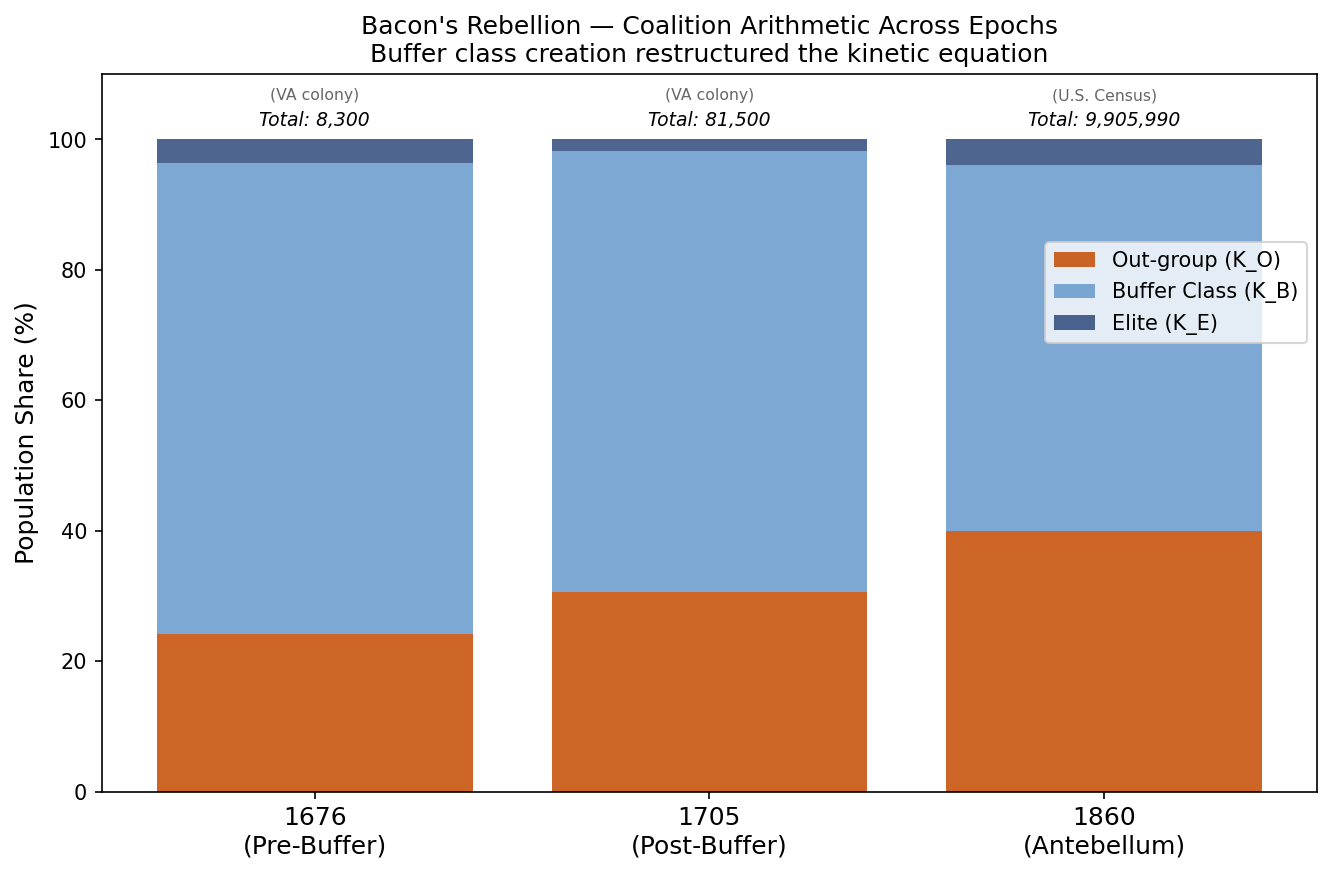
\includegraphics[width=\textwidth]{figures/eq20_24_bacons_rebellion.png}
  \caption{Coalition arithmetic across three epochs: 1676 (pre-Rebellion Virginia), 1705 (post-Slave Code Virginia), and 1860 (antebellum U.S. Census). The stacked bars show the compositional shift in the three-tier population structure. In 1676 the combined servant class overwhelmingly exceeded the elite; after 1705 the buffer class ($K_B$) was legally repositioned to the enforcement side of eq.~\ref{eq:3.5-kinetic-necessary-condition}, making $(K_E + K_B) / K_O \approx 1.5$:1 by 1860.}
  \label{fig:eq20_bacon}
\end{figure}

\paragraph{Comparison to prediction.}
Equation~\ref{eq:3.1-bacon-solidarity-condition} predicts that when $(L_{\text{white}} + L_{\text{black}}) > E$, revolution follows. The anchor case confirms this: the cross-racial coalition burned the colonial capital. Equation~\ref{eq:3.5-kinetic-necessary-condition} predicts that after the coalition was broken, the Elite would restructure enforcement to maintain $K_E + K_B > K_O$ by incorporating $K_B$ (the newly-created Buffer Class) into the enforcement function. The Virginia Slave Codes (1705)---passed within three decades of the rebellion---are the documented implementation of exactly this restructuring: they elevated white labor's legal status, criminalized cross-racial solidarity, and legally deputized the white male population into slave patrol functions, formally allocating $K_B$ to the enforcement side of eq.~\ref{eq:3.5-kinetic-necessary-condition}.

\paragraph{Falsification criteria.}
These equations would be falsified if the historical record showed that the Virginia planter class did not restructure the colony's racial-legal architecture in response to Bacon's Rebellion---i.e., if the cross-racial coalition did not trigger a measurable structural response. The 1705 Virginia Slave Codes constitute direct falsification-resistant evidence: they are a 29-statute legal codification passed within three decades of the rebellion, systematically separating white and Black labor along exactly the axis that the coalition had previously bridged. No alternative explanation for the timing and content of the Codes has been offered by historians that does not invoke the rebellion as the precipitating event.

\paragraph{Confidence tier.}
\textbf{Tier~1 (Anchor Case, $\rho_\tau = 1.0$).} The 1676 event and the 1705 legislative response are among the most extensively documented moments in early American colonial history; Morgan's account is corroborated by Washburn, Breen, and subsequent scholarship. The 1860 arithmetic is drawn directly from Census records. This case serves as the reference calibration point for all subsequent coalition arithmetic comparisons in this study.

\subsection{The Defectors: Empirical Proof That the Complicity Was Chosen}
\label{sec:defectors}

The Necessary Condition Theorem carries a corollary the framework must document honestly: if buffer class complicity was the load-bearing variable, then buffer class members who \textit{refused} that complicity are structurally significant, not merely admirable. Their existence proves the choice was available. The Elite's response to them proves how much was at stake.

The Underground Railroad's white conductor network---Levi Coffin, who facilitated the escape of more than 3,000 people over four decades; Thomas Garrett, a Delaware Quaker who assisted over 2,700 and had his entire estate seized by the courts for it; the networks of Quaker and Methodist stationmasters documented across the free states---constitutes a sustained, organized refusal of the complicity investment. These individuals did not merely decline the psychological wage; they actively deployed their $K_B$ capacity \textit{against} the enforcement function the Elite depended on them to perform.

John Brown's trajectory is the framework's most analytically precise case study. In May 1856, Brown led the Pottawatomie Massacre in Kansas, killing five pro-slavery settlers with broadswords in direct retaliation for pro-slavery violence---a member of $I_{\text{buffer}}$ deploying lethal capacity against the enforcement apparatus rather than on its behalf. In October 1859, Brown led twenty-one men, including five members of $O_{\text{racialized}}$, in the Harper's Ferry raid on the federal armory in Virginia, explicitly attempting to arm the enslaved population and trigger the $M(t) \to \tau$ event the Elite most feared. He was captured by Colonel Robert E.\ Lee, tried not for murder but for \textit{treason}, and hanged in Charles Town, Virginia on December 2, 1859.

The treason charge is the framework's evidence. Murder charges are filed when an individual harms another individual. Treason charges are filed when an individual threatens the \textit{state itself}. The Elite's classification of Brown's actions as treason---the crime reserved for existential threats to the constitutional order---is a direct admission that what he threatened was not a person but the system's operative constraint: $M(t) < \tau$. When a member of $I_{\text{buffer}}$ removes $K_B$ from the enforcement side and redirects it toward liberation, the Elite do not process it as crime. They process it as war.

Thomas Garrett, upon having his estate judicially destroyed, told the Delaware court: ``I say to thee and to all in this courtroom that I never had any money I was so well satisfied with as this.'' He continued operating as a stationmaster until the Civil War. The Elite's graduated response---financial ruin for Garrett, execution for Brown---calibrates precisely to the threat level of the defection. Both responses confirm the same thing: the system understood that buffer class defection was not a peripheral inconvenience. It was an attack on the load-bearing variable.

The framework draws one structural conclusion from this record: the psychological wage was not irresistible. The complicity was chosen. The severity of punishment applied to those who refused it is the clearest available measure of exactly how dependent the extraction kernel was on the buffer class's continued participation.

\subsection{The Complicity Investment: How Witnessed Horror Becomes Lock-in}
\label{sec:complicity_investment}

The Necessary Condition Theorem explains why the Elite needed the buffer class. The Defectors subsection establishes that the complicity was a choice. What remains is the mechanism by which that choice became, for most of $I_{\text{buffer}}$, psychologically irrevocable over time.

The psychological wage ($\psi$) explains recruitment. It does not explain permanence. A worker who accepts a status wage can, in principle, still renounce it---and the pre-1705 record confirms this. The question the framework must answer is not why the Buffer Class initially accepted the contract but why defection became structurally unthinkable across generations.

The answer is the \textbf{Complicity Investment} ($\mathcal{K}_{\text{compl}}$): the accumulation of silent witness to Elite extraction that raises the psychological cost of defection beyond any recoverable threshold. The 1705 contract did not merely grant $I_{\text{buffer}}$ the right to observe the plantation system. It made them \textit{participants in its maintenance}---its patrol riders, its overseers, its enforcers, its witnesses who said nothing. Each act of silence in the face of documented horror is an investment in the perceived necessity of the system. To defect to cross-class solidarity after witnessing what the plantation produced---not abstractly, but concretely, across the fence line, inside the same community---is to confront not only the injustice of the system but one's own position within it.

The critical variable is the prior solidarity. Before 1705, this was not a population of strangers. These were people who had run away together, eaten together, planned rebellion together, and in documented cases formed families together---the 1691 boundary enforcement statute (Section~3.3.4) was enacted precisely because the crossing was occurring. The complicity that followed 1705 was therefore not the passive acceptance of a stranger's exploitation. It was the deliberate abandonment of known people---whose faces were recognizable, whose children were named---to a system of extraction whose full horror became visible from close range over generations of uninterrupted proximity.

The depth of the betrayal is proportional to the depth of the prior solidarity. This is not incidental: it is the architecture. The Elite required the complicity investment to function at maximum lock-in. A buffer class that had never known solidarity with the out-group could, in principle, discover it. A buffer class that had known it---and then watched anyway---cannot recover that possibility without dismantling the psychological structure they have spent generations building to live with what they witnessed. The system's most efficient lock-in mechanism is not the wage it pays. It is the atrocity it makes the buffer class watch in silence.

\begin{tcolorbox}[colback=white, colframe=black!55, fonttitle=\bfseries\small, title=Author's Note]
\small
There is an argument that the preceding analysis should be delivered in purely formal terms---that the set-theoretic apparatus renders the emotional register unnecessary, even distracting. I have considered this argument and rejected it.

The historical record documented in this chapter---the Thistlewood diaries, the infant boiled for refusing to eat, the 500 documented lashes on Elizabeth Abbott's body, the children auctioned while their mothers watched---is not data that can be adequately handled by notation alone. W.E.B.\ Du~Bois, in \textit{Black Reconstruction in America}, understood this. He did not choose between rigorous historical analysis and moral clarity. He insisted they were the same operation.

What this chapter formalizes as the ``Complicity Investment'' is, in human terms, something that should be named directly: a population that watched those things happen, in their own communities, to people they had recently known as equals---and chose, generation after generation, the status wage over solidarity---participated in one of the most consequential betrayals in the history of human organization. The framework does not require the reader to feel this. It requires the reader to understand it structurally. But the author is not neutral on the question of what this cost, and pretending otherwise would be its own form of distortion.

The men and women of the Underground Railroad, John Brown on the scaffold at Charles Town, the Polish soldiers who defected at Saint-Domingue---these were not anomalies demonstrating that individual goodness can transcend structural pressure. They were proof that the choice existed. That so many others made the different choice is the subject of this chapter. That the system was engineered to make that choice feel inevitable is its central argument.
\end{tcolorbox}

\section{The Johnson Theorem: Empirical Confession of the Algorithm}

To prove that the Predatory Min-Max Function is not merely a retrospective academic theory but the conscious, operational strategy of the political class, we must examine the explicit confessions of those within $P_{\text{uppet}}$. The most devastating articulation of this algorithmic manipulation was provided by President Lyndon B.\ Johnson in 1960.

In a moment of unvarnished candor regarding Southern political strategy, Johnson outlined the exact mechanics of Elite extraction:

\begin{quote}
\textit{``If you can convince the lowest white man he's better than the best colored man, he won't notice you're picking his pocket. Hell, give him somebody to look down on, and he'll empty his pockets for you.''}
\end{quote}

Translated into the formal set-theoretic framework of this book, Johnson's statement perfectly maps the five-tier extraction engine:

\medskip
\noindent\textbf{``Convince the lowest white man he's better than the best colored man\ldots''}

\noindent This is the deliberate deployment of the psychological wage ($\psi$). The Puppet Class ($P_{\text{uppet}}$) artificially elevates the social status of the Buffer Class ($I_{\text{buffer}}$) by contrasting them against a subjugated Out-group ($O_{\text{racialized}}$). It is a mathematically zero-cost transaction for the Elite; they grant superiority in \textit{status} to avoid granting equality in \textit{capital}.

\medskip
\noindent\textbf{``\ldots he won't notice you're picking his pocket.''}

\noindent This is the hidden extraction kernel. While $I_{\text{buffer}}$ is entirely focused on policing the social boundary and enjoying their psychological wage, the Elite ($E$) is actively extracting material wealth from them. The ideological justification of racism acts as a systemic sleight-of-hand, blinding the Buffer Class to their own economic exploitation.

\medskip
\noindent\textbf{``Hell, give him somebody to look down on, and he'll empty his pockets for you.''}

\noindent This is the ultimate triumph of the Agenda-Setter Trap (Section~5.6). Johnson reveals that the psychological wage is so profoundly addictive that $I_{\text{buffer}}$ will not only ignore their own exploitation---they will actively \textit{finance} it. By maintaining the Out-group as a target for derision and fear, the Elite mathematically guarantees that the Buffer Class will continuously vote against their own material interests, voluntarily transferring their wealth upward to $E$ to maintain the illusion of supremacy.

\medskip
The ``Johnson Theorem'' serves as the definitive proof that systemic racism is not driven by irrational, spontaneous hatred from the working class. It is a highly rational, top-down economic mechanism engineered by $E$ and executed by $P_{\text{uppet}}$ to ensure that the In-group remains docile, distracted, and eager to be robbed.
\section{Racism as Trojan Horse: Undermining the Constitution's Anti-Classist Framework}

The American Framers created a constitutional framework with explicitly anti-classist elements: prohibition of titles of nobility (Article I, Sections 9-10), grounding rights in ``the people'' rather than aristocratic privilege, and establishing equal protection principles. However, \textbf{the Framers had to compromise the democracy they were creating to uphold slavery}, introducing deliberate \textbf{contradictions}---``bugs in the source code''---that would allow the Elite to maintain class hierarchy while appearing to establish egalitarian governance.

These bugs were not accidental flaws but \textit{features} designed to preserve slave capitalism, and they have allowed American democracy to \textit{decay over time} as each generation exploits the same loopholes to expand the subjugated class.

\textbf{The Five Constitutional Bugs}

\begin{enumerate}
    \item \textbf{``We the People'' (undefined)}: Deliberately leaves this term undefined---creating a variable that can be narrowed to exclude disfavored groups. A deliberate vulnerability, not ambiguity.
    
    \item \textbf{No titles of nobility (with exception)}: Prohibits hereditary aristocracy but permits hereditary enslavement by framing it as property law rather than title law.
    
    \item \textbf{Equal representation (with inequality)}: One person, one vote---but counts enslaved people as 3/5 for apportionment while denying them personhood, embedding inequality into the equality mechanism.
    
    \item \textbf{Due process (with property exception)}: Protects against deprivation of ``life, liberty, or property''---but defines enslaved people as property, making the protection become the mechanism of oppression.
    
    \item \textbf{Commerce clause (enabling slave trade)}: Prohibits banning slave importation until 1808, explicitly protecting slave capitalism and establishing precedent that economic interests override human rights.
\end{enumerate}

These engineered vulnerabilities allow slave capitalism to persist within a framework claiming to oppose aristocracy.

\textbf{Dred Scott: Exploiting Bug \#1}

In \textit{Dred Scott v.\ Sandford} (1857), Chief Justice Taney demonstrated how Bug \#1 (undefined ``the people'') could be exploited \cite{dredscott, fehrenbacher}. He excluded Black people from ``the people,'' declaring they ``had no rights which the white man was bound to respect,'' explicitly noting that inclusion would mean they could ``keep and carry arms wherever they went''---an outcome Taney characterized as inevitably ``endangering the peace and safety of the State.'' \textit{Dred Scott}, 60 U.S.\ at 416--417.

This revealed the four-step mechanism:
\begin{enumerate}
    \item Define racial classifications as natural facts (not social constructions)
    \item Exclude racialized groups from ``the people''
    \item Strip constitutional rights (rights depend on being among ``the people'')
    \item Evade anti-classist protections (frame as ``racial,'' not class-based)
\end{enumerate}

As the constitutional analysis brief notes: ``The phrase 'the people' is the constitutional hinge. If courts can narrow that definition... then every right dependent on that phrase becomes conditional. Conditional rights are not rights at all; they are privileges dispensed by the state.''

\textbf{The Pattern of Expansion and Democratic Decay}

Once these bugs existed, each generation exploited them to expand control:

\begin{itemize}
    \item \textbf{Bug \#1 (undefined ``the people'')}: Used by \textit{Dred Scott} to exclude Black people $\rightarrow$ now excludes felons, immigrants, political opponents
    \item \textbf{Bug \#4 (due process exception)}: Used to justify slavery $\rightarrow$ now justifies civil asset forfeiture, economic inequality
    \item \textbf{Bug \#5 (commerce primacy)}: Protected slave trade $\rightarrow$ now prioritizes corporate interests over human rights
\end{itemize}

\paragraph{Bug \#4 in the federal code.} The modern exploitation of the due process exception is codified in \usclink{apx:usc:18:981a}{18 U.S.C.~\S~981}, which authorizes the federal government to seize property without a criminal conviction:
\uscinline{usc_18_981a}

The result: mass incarceration creates a ``criminal'' class excluded from ``the people''; economic policies concentrate wealth while dividing the working class along racial lines; surveillance state expansion by designating groups as ``dangerous''; gun control using \textit{Dred Scott}'s logic to narrow ``the people.''

\begin{figure}[htbp]
\centering
\begin{tikzpicture}[
    bug/.style={draw, thick, rounded corners=2pt, minimum height=0.7cm, minimum width=3.8cm, align=left, font=\footnotesize, anchor=west},
    exploit/.style={draw, thick, rounded corners=2pt, minimum height=0.7cm, minimum width=4.5cm, align=left, font=\footnotesize, anchor=west},
    arr/.style={->, thick, >=stealth, red!60},
    scale=0.88, transform shape
]
    % Headers
    \node[font=\small\bfseries, anchor=west] at (-0.2,5.5) {Constitutional Provision};
    \node[font=\small\bfseries, anchor=west] at (6.0,5.5) {Exploitation Pathway};

    % Bug 1
    \node[bug, fill=blue!10] (b1) at (0,4.5) {\textbf{\#1} ``We the People'' (undefined)};
    \node[exploit, fill=red!10] (e1) at (6.2,4.5) {\textit{Dred Scott} $\rightarrow$ felons $\rightarrow$ immigrants};
    \draw[arr] (b1.east) -- (e1.west);

    % Bug 2
    \node[bug, fill=blue!10] (b2) at (0,3.4) {\textbf{\#2} No titles of nobility};
    \node[exploit, fill=red!10] (e2) at (6.2,3.4) {Hereditary slavery as ``property law''};
    \draw[arr] (b2.east) -- (e2.west);

    % Bug 3
    \node[bug, fill=blue!10] (b3) at (0,2.3) {\textbf{\#3} Equal representation};
    \node[exploit, fill=red!10] (e3) at (6.2,2.3) {3/5 Compromise $\rightarrow$ disproportionate power};
    \draw[arr] (b3.east) -- (e3.west);

    % Bug 4
    \node[bug, fill=blue!10] (b4) at (0,1.2) {\textbf{\#4} Due process protection};
    \node[exploit, fill=red!10] (e4) at (6.2,1.2) {Property = persons $\rightarrow$ asset forfeiture};
    \draw[arr] (b4.east) -- (e4.west);

    % Bug 5
    \node[bug, fill=blue!10] (b5) at (0,0.1) {\textbf{\#5} Commerce clause};
    \node[exploit, fill=red!10] (e5) at (6.2,0.1) {Slave trade protected $\rightarrow$ corporate primacy};
    \draw[arr] (b5.east) -- (e5.west);

    % Annotation
    \node[font=\scriptsize, gray, align=center] at (5.5,-0.7) {Each ``bug'' was not a flaw but a \textit{feature}---designed to preserve slave capitalism\\within a framework claiming to oppose aristocracy.};
\end{tikzpicture}
\caption{\textbf{The Five Constitutional Bugs: Provision vs.\ Exploitation.} Each constitutional provision (left) contains a deliberate vulnerability that enables the Elite to maintain class hierarchy through racial mechanisms (right). The arrows trace the exploitation pathway from original framing to contemporary application.}
\label{fig:constitutional_bugs}
\end{figure}

These vulnerabilities, which we formalize as ``Constitutional Bugs,'' provided the Elite with the necessary exploits to maintain the extraction engine within a framework claiming to oppose aristocracy (see Figure~\ref{fig:constitutional_bugs}).

\textbf{The Ehrlichman Admission: Proof of Deliberate Engineering}

The deliberate nature of this Out-group engineering was confirmed by John Ehrlichman, Nixon's domestic policy adviser, in a 1994 interview published two decades later:

\begin{quote}
\textit{``The Nixon campaign in 1968, and the Nixon White House after that, had two enemies: the antiwar left and black people. You understand what I'm saying? We knew we couldn't make it illegal to be either against the war or black, but by getting the public to associate the hippies with marijuana and blacks with heroin, and then criminalizing both heavily, we could disrupt those communities. We could arrest their leaders, raid their homes, break up their meetings, and vilify them night after night on the evening news. Did we know we were lying about the drugs? Of course we did.''} \cite{baum}
\end{quote}

This admission is extraordinary because it confirms every element of the algorithmic model: the Elite \textit{deliberately} engineered the association between a racial group and a criminal category, \textit{knowing} the pretext was fabricated, in order to narrow ``the people'' by expanding the ``criminal'' class. The War on Drugs was not a policy failure---it was Bug~\#1 being exploited with surgical precision. Mass incarceration did not \textit{accidentally} create a new Out-group; it was \textit{designed} to do so, using the 13th Amendment's exception clause as the legal kernel (Section~4.4).

\textbf{The Suppression of Medical Consensus}

The fabrication Ehrlichman describes required \textit{overwriting established scientific truth}. Cannabis was not a marginal folk remedy but a mainstream pharmaceutical: it appeared in the \textit{United States Pharmacopoeia} from 1850 to 1942 and was prescribed by leading physicians of the era. Sir William Osler, widely regarded as the father of modern medicine, recommended cannabis as the most effective treatment for migraine in his landmark \textit{Principles and Practice of Medicine} \cite{osler}. When Congress held hearings on the Marihuana Tax Act of 1937, the American Medical Association's legislative counsel, Dr.\ William C.\ Woodward, testified in opposition, objecting that the bill's use of the unfamiliar term ``marihuana'' had deliberately obscured the fact that Congress was outlawing a well-known medicine. Woodward warned that prohibition would cripple medical research---a prediction borne out by decades of suppressed investigation \cite{musto, bonnie}.

The committee's response to the AMA's objection is instructive: Woodward was accused of obstruction and dismissed. The Marihuana Tax Act passed with virtually no debate. This episode reveals the Variable Swap in its epistemic dimension: the system did not merely criminalize a substance but \textit{manufactured ignorance} about it. A drug with centuries of documented therapeutic use was rebranded using an unfamiliar Spanish-language term (``marihuana'') to sever it from its medical identity, then associated with racialized populations---Mexican immigrants and Black jazz musicians---to generate the moral panic necessary for prohibition \cite{bonnie}. The proxy variable $P$ was not discovered in nature; it was \textbf{engineered against the explicit objections of the medical establishment}, demonstrating that ideological justification (Component 3 of the architecture) can override even authoritative scientific consensus when $E$'s extraction objectives require it.

\textbf{Why This Works: Racism as Elite Class Maintenance}

The genius of using racism to undermine anti-classist protections:
\begin{enumerate}
    \item \textbf{Appears natural}: Racial categories framed as biological facts, not social constructions serving Elite interests
    \item \textbf{Evades scrutiny}: Constitutional prohibitions on class hierarchy don't apply to ``natural'' racial differences. Lee Atwater, architect of the Republican Southern Strategy, made this mechanism explicit in a 1981 interview:

    \begin{quote}
    \textit{``You start out in 1954 by saying, `Nigger, nigger, nigger.' By 1968 you can't say `nigger'---that hurts you, backfires. So you say stuff like, uh, forced busing, states' rights, and all that stuff, and you're getting so abstract. Now, you're talking about cutting taxes, and all these things you're talking about are totally economic things and a byproduct of them is, blacks get hurt worse than whites.''} \cite{atwater}
    \end{quote}

    Atwater's admission is the Predatory Min-Max Function described in plain language. The transition from explicit racial slurs to ``abstract'' economic policy is precisely the \textbf{Variable Swap} formalized in Section~6.2: the system's \textit{interface} changes (from overt racism to ``race-neutral'' policy language) while the \textit{kernel} remains identical (policies engineered to disproportionately harm the Out-group). The ``byproduct'' Atwater describes is not incidental---it \textit{is} the function. The abstraction provides plausible deniability, ensuring that constitutional prohibitions on class hierarchy are never triggered because the policy never names race, even as it targets racialized communities with mathematical precision.
    \item \textbf{Divides resistance}: Working-class whites invested in racial hierarchy, preventing cross-racial solidarity
    \item \textbf{Provides precedent}: Narrowing ``the people'' creates legal mechanisms for future exclusions
    \item \textbf{Protects Elite power}: Fundamental class hierarchy remains hidden beneath racial division
\end{enumerate}

The Framers sought to prevent hereditary aristocracy but left open the mechanism by which the Elite could recreate class hierarchy through racial categorization. Slave capitalism required this constitutional loophole, and racism provided it. The democracy \textit{rots from within} because these bugs cannot be patched without fundamental restructuring.

This reveals how racism was \textbf{deliberately engineered by Elites to break class solidarity and create an exploitable labor class unconstrained by moral limits}, while also weaponizing constitutional vulnerabilities to undermine protections that might have constrained Elite power. The constitutional bugs transform anti-classist principles into hollow promises by narrowing ``the people'' to exclude disfavored groups---a mechanism still actively exploited today.

\section{The Second Crash and the Constitutional Patch: The Prototype Puppet Class (1787)}

The invention of the Buffer Class in 1705 solved the immediate crisis of cross-racial solidarity, but it did not solve the Elite's deeper vulnerability: \textit{visibility}. As long as the Elite ruled directly---as kings, royal governors, and landed aristocracy---they remained the obvious target whenever the system produced suffering. If the Buffer Class starved, they knew exactly whose mansion to burn.

Shays' Rebellion (1786--1787) served as the second ``crash report'' in the Elite's operating system. Barely a decade after independence, armed farmers in Massachusetts---members of the very Buffer Class that was supposed to be pacified---rose up against debt collectors and courts. The rebellion terrified the Elite precisely because it demonstrated that the Buffer Class, despite their psychological wages, could still identify the economic source of their suffering.

The Elite's solution was architectural: \textbf{separate the front-end from the back-end}. Rather than ruling directly, they would engineer a system of representative government---a political \textit{interface}---that the Buffer Class and Out-group would interact with, vote for, direct their grievances toward, and ultimately blame when the system failed. Meanwhile, the Elite would retreat to the back-end: managing the capital, the land, the central banks, and the true levers of power, entirely insulated from democratic accountability.

The Constitutional Convention of 1787 was this architectural separation made concrete. The ``Prototype Puppet Class'' ($P_{\text{uppet}}^{\text{v1.0}}$) was deployed: a Representative Republic where elected officials served as the visible face of governance while the true parameters of the system---property law, commerce, monetary policy---remained under Elite control.

The initial ``Algorithmic Filter'' was crude but effective: only white male property owners were legally permitted to vote or hold office. This ensured that the first generation of the Puppet Class was drawn almost entirely from the Elite themselves or their direct proxies. But the architecture was designed to scale. The system did not require the Elite to personally occupy every seat of power; it merely required that whoever occupied those seats remained tethered to Elite capital.

The Convention also embedded a critical exploitation variable directly into the constitutional source code: the \textbf{Three-Fifths Compromise}. Slave states were permitted to count enslaved people---who possessed no legal personhood, no rights, and no political agency---as three-fifths of a person for purposes of congressional apportionment. This gave the slave-holding Elite disproportionate political representation powered by the very bodies they owned. The Out-group was simultaneously denied humanity \textit{and} weaponized as political capital for the Elite. It was the first instance of the system using the Out-group's biological existence as a mathematical input to amplify Elite power---a logic that would later recur in the Demographic Paradox (Section~6.6).

This constitutional patch created the illusion of self-governance while mathematically guaranteeing that the extraction kernel remained untouchable. The Elite no longer wore crowns; they funded representatives. And when the people grew angry, they directed their fury at the representatives---the front-end---while the back-end continued to extract, undisturbed.

The Constitutional Patch preserved $\Delta\max = 0$ in the sense established in Chapter~\ref{ch:redefining}: the federal architecture did not finance $I_{\text{buffer}}$ stability or slave-state political advantage by reducing $E$'s take; it financed them by embedding deeper extraction from $O_{\text{racialized}}$ directly in the supreme law---most visibly through the Three-Fifths apportionment rule and the Fugitive Slave Clause, which extended the racial partition and the property form of the enslaved across state lines. Read against the ``compromise'' framing, these clauses are not evidence that the Framers split the difference with justice; they are evidence that the concession cost was routed through $O_{\text{racialized}}$, leaving $E$'s net position non-decreasing as a result of the bargain.

\section{The Haitian Catalyst and the Spatial Expansion of the Algorithm (1803)}

The destruction of the French colonial machine in Saint-Domingue had a direct, systemic consequence for the architecture of the United States. Napoleon Bonaparte’s loss of his most profitable extraction zone—and the defeat of his armies by the Indigenous Army of formerly enslaved Haitians—forced France to abandon its North American empire, culminating in the 1803 Louisiana Purchase.

For the American Elite ($E_{US}$), the Haitian victory provided the ultimate spatial expansion for their domestic extraction algorithm. The acquisition of the Louisiana Territory doubled the size of the United States. This vast new geography was immediately utilized to scale the institution of chattel slavery to unprecedented industrial levels.

Crucially, this expansion fortified the domestic Buffer Class ($I \setminus E$). By opening millions of acres of stolen Indigenous land to poor white settlers, the Elite effectively expanded the psychological and material "wages of whiteness." The American In-group was given a vested interest in moving westward and defending the expansion of the slave economy. Thus, the successful liberation of the Out-group in Haiti inadvertently provided the American Elite with the geographic fuel required to optimize the Predatory Min-Max Function for another sixty years.

\section{The Haitian Contagion and the Algorithmic Lockdown}
\label{sec:haitian_contagion}

The absolute liberation of the Out-group in Saint-Domingue ($O_{\text{emancipated}}$) presented an existential threat to the American Elite ($E_{US}$). The Haitian Revolution proved that the Predatory Min-Max Function could be violently overturned if the subjugated class achieved operational solidarity. This was not a theoretical anxiety; the "Haitian Contagion" directly inspired a wave of domestic resistance, most notably Gabriel Prosser’s Rebellion in Virginia (1800) and the massive German Coast Uprising in Louisiana (1811), the latter of which was heavily populated by individuals directly influenced by the Haitian diaspora.

To prevent a total system collapse, the Elite required an immediate, aggressive update to the domestic control matrix. They executed an "Algorithmic Lockdown" by passing a rapid succession of state and federal laws—proxy variables ($P$) specifically engineered to neutralize the vectors of revolution: communication, movement, and education.

\begin{enumerate}
    \item \textbf{The Information Quarantine ($P_{\text{literacy}}$ and $P_{\text{assembly}}$)}: The Elite recognized that revolution requires the transmission of ideas. Consequently, Southern legislatures systematically criminalized the transfer of information. Laws were passed making it a severe criminal offense to teach any Black person (enslaved or free) to read or write. Furthermore, independent Black assembly was outlawed; all religious gatherings or social meetings required the presence of white overseers. By forcing the Out-group into an enforced state of illiteracy and isolation, the system structurally severed their ability to coordinate mass resistance.
    
    \item \textbf{Quarantining the Free Out-Group ($P_{\text{containment}}$)}: The existence of a free, mobile Black population contradicted the system’s core ideological justification (Component 3) and posed a massive security risk. Following the Haitian victory and the thwarted Denmark Vesey rebellion (1822) in South Carolina, the Elite engineered laws like the Negro Seamen Acts.
    
    These laws required that any free Black sailor arriving in a Southern port be immediately arrested and held in the local jail for the entire duration their ship was docked. If the ship's captain failed to pay the jail fees upon departure, the free Black sailor was sold into slavery. This was a highly efficient extraction mechanism: it physically quarantined individuals who might bring news of Haitian liberation, intimidated the free Out-group, and provided a legal mechanism to drag autonomous Black individuals back into the biological extraction pool.
    
    \item \textbf{Weaponizing the Buffer Class via the Complicity Trap}: Crucially, this legislative lockdown was activated not merely through propaganda but through a mechanism far more structurally precise---the Complicity Trap. The Elite did not need to manufacture a fear from nothing. They had already manufactured the conditions under which the fear would be partially real. The full analysis of this mechanism follows immediately below.
\end{enumerate}

\subsection{The Complicity Trap: Giving the Buffer Class Skin in the Game}
\label{sec:complicity_trap}

The ``Black Jacobin'' paranoia that swept the antebellum South was not, strictly speaking, irrational. This is the analytical point the framework must handle with precision. The Elite did not merely sell the buffer class an unfounded fear. They first \textit{engineered the conditions under which the fear would be partially justified}, and then used Haiti to activate it.

The mechanism operates in sequence. Prior to 1791, the Buffer Class occupied a structurally complicit position. They were not passive beneficiaries of a distant extraction system. They were the slave patrol riders. They were the witnesses to the Thistlewood-documented horrors---the boiled infants, the ``Darby's doses,'' the whippings recorded across thousands of pages of plantation diaries---happening in their own communities, across their own fence lines. They were the population that had, only decades prior, eaten with, fought beside, fled alongside, and in documented cases formed families with the same people now subjected to this system (see Section~3.3.4). The complicity investment (Section~\ref{sec:complicity_investment}) had been paid in full by the time Toussaint Louverture's army burned the northern plain of Saint-Domingue.

When news of the revolution arrived, the Elite did not need to construct a lie from nothing. They needed only to point. The fear was effective precisely because the Buffer Class could not honestly claim neutrality. A genuinely uninvolved bystander can be reassured that a revolution targets the enslavers and not them. The Buffer Class---which had patrolled, recaptured, witnessed, and said nothing for generations---could not make that claim. Their own accurate self-assessment of their structural position made the fear credible: \textit{I know what was done. I know what I am to them.}

The Elite's message, transmitted through the press, the pulpit, and the political apparatus, was not a fabrication but a weaponized acknowledgment of the complicity the Elite had themselves engineered: \textit{You have skin in the game now. You watched. You patrolled. You enforced. If they rise the way Haiti rose, they are not only coming for us---they are coming for everyone who stood by while it happened.} The Buffer Class did not need to be persuaded this was unfair. They needed to be persuaded that their only protection was the system that had made them complicit. And the Elite, by deploying the complicity investment before deploying the Haitian fear, had ensured that no other logical conclusion was available to them.

This is the Complicity Trap: a population made genuinely complicit in atrocities cannot be liberated from the system that produced those atrocities without first confronting what it participated in. The psychological cost of that confrontation is so high that the system can depend on the Buffer Class to suppress it indefinitely---not because the Buffer Class is uniquely evil, but because the alternative to suppression is unbearable.

\paragraph{The modern instantiation.}
The Complicity Trap does not require living memory. It transmits generationally as a form of fear the framework must distinguish carefully from guilt. \textbf{Guilt} is the affective response to one's own actions: it is processable through confession, apology, and the reassurance that the individual did not personally commit the atrocity. \textbf{Fear}, as the framework uses the term here, is the structural response to documented evidence: \textit{if the full historical record were widely known and treated as a legitimate basis for accountability, a claim to reckoning would become valid.} Guilt says: \textit{I would rather not think about this.} Fear says: \textit{if they understand what was done, the logic of accountability becomes sound.}

This distinction resolves an apparent puzzle in contemporary politics. The intensity of the sustained campaign against accurate historical education---legislative bans on curriculum, book removal, the criminalization of pedagogical frameworks labeled ``critical race theory''---is not proportional to embarrassment. People do not pass emergency statutes to manage embarrassment. They pass emergency statutes to prevent conditions they perceive as threatening. The suppression of accurate historical education is not primarily a shame-management operation. It is a \textbf{reckoning-prevention operation}: a system-level response to the causal chain that runs from \textit{documented atrocity} $\rightarrow$ \textit{legitimate grievance} $\rightarrow$ \textit{justified accountability}. The Complicity Trap that the Elite installed in the antebellum period is still running. Its modern interface is a school board meeting and a legislative chamber. The mechanism is identical: suppress the historical record, and accountability cannot find its footing.

\section{The Sovereign Ransom and the \texorpdfstring{$P_{\text{debt}}$}{P\_debt} Variable}

When an Out-group successfully achieves absolute physical autonomy ($O_{\text{emancipated}}$)—as occurred with the Haitian Revolution (1791 -- 1804)—the Elite ($E$) experiences a catastrophic system failure. The biological capital is lost. However, the global architecture of oppression is highly adaptive. If physical labor cannot be extracted, the system will pivot to extracting sovereign wealth through a newly engineered proxy variable: sovereign debt ($P_{\text{debt}}$).

In 1825, backed by a blockade of heavily armed warships, France forced the newly independent Republic of Haiti to pay 150 million francs (later reduced to 90 million) to compensate French plantation owners for the "loss" of their enslaved laborers. Mathematically, the global Elite ($E_{\text{global}}$) engineered a scenario where the Out-group was forced to literally purchase their own bodies and stolen autonomy at gunpoint.

This Independence Debt functioned identically to the domestic systems of convict leasing or modern carceral bonds; it ensured a continuous, multi-generational flow of capital from the Out-group directly into the central banks of the Elite (first France, and later Wall Street). By forcing Haiti to dedicate up to 80\% of its national budget to debt service until 1947, the system permanently locked the nation into an economically degraded state ($O_{\text{degraded}}$), proving that the extraction algorithm can seamlessly translate biological enslavement into financial subjugation.


\part{The Installation (1619--1865)}
\label{part:installation}

\chapter{The Haitian Export: Hemispheric Liberation, Vexillological Contagion, and the Firmin Protocol (1803--1915)}
\label{ch:haitian_export}

\begin{tcolorbox}[colback=black!5, colframe=black!70, fonttitle=\bfseries\ttfamily,
  title=RUNTIME LOG: HAITI (1803--1915 CE){,} OUT-GROUP EXPORT VECTOR ACTIVE]
\ttfamily\small
\textbf{System Stress} ($\min$: containment integrity): ACCELERATING FAILURE --- $O_{\text{emancipated}}$ has achieved kinetic kernel termination. Haitian Theorem executed at $\rho_{\tau} = 1.0$ (Chapter~\ref{ch:contradiction}). Export vector active: arms, munitions, sanctuary, and diplomatic recognition flowing outward to Gran Colombia, Mexico, Dominican Republic, and Greece. Regional extraction infrastructure fracturing.\\
\textbf{Capital} ($\max$: extraction output): DEFENSIVE --- Saint-Domingue revenue stream terminated (Pearl of the Antilles offline). Caribbean extraction under existential contagion threat. $E_{\text{global}}$ shifting to secondary extraction modes: $P_{\text{debt}}$ variable queued.\\
\textbf{Interference State} ($\Phi_{\text{load}}$, proximity to $\tau$): MAXIMAL FOR $E_{\text{global}}$ --- Sovereign Black republic broadcasting proof-of-concept to every enslaved population in the hemisphere. Estimated $\rho_{\tau} \in [0.70, 0.90]$ for adjacent Caribbean extraction zones.\\
\textbf{Active Patch}: DEPLOYING --- (1) Diplomatic embargo: U.S. refusal to recognize Haiti until 1862. (2) $P_{\text{debt}}$ deployed: 90 million franc indemnity (1825), compounded by CIC private-bank interest (1825--1947). (3) Algorithmic lockdown: Negro Seamen Acts, literacy bans, criminalization of Haitian news transmission. (4) $F_{\text{enforce}}$ override: U.S. military occupation (1915--1934), corv\'{e}e reinstated.\\
\textbf{Counter-Vector} ($O_{\text{emancipated}}$): EXECUTING --- Pétion–Bolívar arms transfer (1815--1816); Mina expedition supply (1816--1817); Geffrard cross-border support for Dominican Restoration (1863--1865); Boyer diplomatic recognition of Greece (1822). Vexillological contagion encoded in six flag lineages across the Americas. Firmin Protocol deployed at Môle Saint-Nicolas (1891): fleet repelled without a single shot.\\
\textbf{Result}: \textbf{[PARADOX]} $E_{\text{global}}$ successfully degrades Haiti economically ($O_{\text{degraded}}$ by 1947). But the export vectors have already fractured the Spanish Empire and encoded the liberatory signature permanently in the political geography of the Western Hemisphere. The contagion is structurally irreversible.
\end{tcolorbox}

\medskip

The preceding chapter closed with three interlocking accounts of how the global Elite ($E_{\text{global}}$) responded to Haiti's 1804 emancipation: the Haitian Catalyst that accidentally gifted the American Elite a continental expansion zone (Section~\ref{sec:haitian_contagion}); the Algorithmic Lockdown engineered to prevent the contagion from replicating domestically; and the Sovereign Ransom that weaponized debt to extract from a people the battlefield could not subjugate. Those sections document the Elite's \textit{containment response} to the Haitian breach.

This chapter documents the \textit{dual}: what the newly sovereign Out-group ($O_{\text{emancipated}}$) did with its autonomy while the Elite attempted containment. The answer is structurally remarkable. Rather than retreating into defensive isolation, the Republic of Haiti actively weaponized its sovereignty---deploying arms, munitions, veterans, sanctuary, diplomatic recognition, and ultimately its own flag geometry---in a sustained campaign to fracture the extraction zone that surrounded and threatened it. The Haitian export was not charity. It was strategic self-defense executed through the only leverage available to a newly liberated state surrounded by hostile, slave-holding empires: the export of the revolution itself.

If the Atlantic racial order is a fractal mind virus, Haiti is the first successful counter-virus to execute at state scale. Its danger was not only military. It proved, in public and in color, that the racial prior was false: the supposedly extractable population could defeat the empire, govern itself, arm other revolutions, and reason strategically about hemispheric power. That proof threatened the host wetware of the imperial core, which is why the response had to target not only Haitian territory but also Haitian news, literacy, sailors, flags, debt, and diplomatic recognition.

%─────────────────────────────────────────────────────────────────────
\section{The Inverse Contagion: From Quarantine Target to Active Vector}
\label{sec:inverse_contagion}
%─────────────────────────────────────────────────────────────────────

Section~\ref{sec:haitian_contagion} established the Elite's reading of Haitian independence as a pathogen requiring quarantine. The Haitian Revolution had proven that the Predatory Min-Max Function---$\max$ capital extraction, $\min$ unified resistance---was not mathematically invincible. It could be violently overturned when the subjugated class achieved operational solidarity. This was not an abstraction. It was a documented execution. The Elite's immediate response was therefore to treat Haiti as a contagion source: the diplomatic embargo, the Negro Seamen Acts, the criminalization of Black literacy, the Complicity Trap of Section~\ref{sec:complicity_trap}---all were containment measures directed at preventing the Haitian proof-of-concept from replicating.

What this containment framing obscures is the agency of the source itself. The Haitian Theorem (Chapter~\ref{ch:contradiction}) establishes that kinetic action is the only historically validated liberation mechanism at the colonial scale. What the theorem does not predict---but what the historical record confirms---is what a sovereign Out-group does \textit{after} it executes that kinetic action. The answer, in Haiti's case, is that it immediately began exporting it.

The structural logic was not idealistic. The early Haitian heads of state---Dessalines, Henri Christophe, and most consequentially Alexandre Pétion---understood with mathematical precision that their republic's long-term survival depended on the dismantling of the extraction zone that surrounded it. As long as the adjacent territories of Cuba, Jamaica, Venezuela, Colombia, and Saint-Domingue's eastern neighbor remained slave-holding extraction zones under European imperial control, Haiti remained encircled by hostile powers whose economic interests demanded either Haiti's reconquest or its permanent degradation into a cautionary tale. The only viable defense was offense: fracture the surrounding extraction zone by exporting the revolution to it.

This is the ``Inverse Contagion''---not the passive spread of revolutionary ideology that the Elite feared and tried to suppress, but the \textit{active, material, condition-bearing export} of liberation capacity. Where the Elite's containment apparatus functioned as a \textit{cordon sanitaire} designed to quarantine the pathogen, the Haitian state functioned as a \textit{deliberate inoculation program}, injecting revolutionary capacity into adjacent movements with a specific political price tag: the abolition of slavery as the non-negotiable condition of Haitian support. The export was not performed at random. It was a foreign policy---the first coherent anti-colonial foreign policy in the history of the Americas.

This chapter analyzes that policy across four operational theaters: the material underwriting of South American independence (Section~\ref{sec:petion_condition}); the geometric encoding of revolutionary solidarity in the flags of the Americas (Section~\ref{sec:vexillological_contagion}); the deployment of legal expertise as a diplomatic weapon against U.S. naval coercion (Section~\ref{sec:firmin_protocol}); and the mechanics of the financial double-debt that the Elite eventually deployed to neutralize the export's economic engine (Section~\ref{sec:cic_double_debt}).

%─────────────────────────────────────────────────────────────────────
\section{The Consumptive Extraction Function: Quantifying the Kernel Haiti Destroyed}
\label{sec:consumptive_function}
%─────────────────────────────────────────────────────────────────────

To measure what the Haitian export accomplished, it is necessary first to quantify what was destroyed when the Haitian Revolution terminated the plantation kernel. The Caribbean extraction zone operated on what this framework calls the \textbf{Consumptive Extraction Function}: a production model that optimized for maximum caloric and physical output over the shortest possible biological duration, treating enslaved human life as an infinitely replenishable input rather than a capital asset requiring preservation.

Between the early sixteenth century and the late nineteenth century, an estimated 12.5 million enslaved Africans were loaded onto transatlantic slave ships; approximately 10.7 million survived the Middle Passage \cite{james_black_jacobins}. The geographic distribution of these captives reveals the Caribbean's structural primacy within the extraction hierarchy. While British North America---the territory that became the United States---absorbed roughly 3.5 percent of the transatlantic trade, the Caribbean colonies absorbed approximately 35 percent, with Brazil accounting for another 40 percent \cite{james_black_jacobins}. The Caribbean's outsized claim on the trade reflects its role as the system's highest-intensity production zone.

The Consumptive Extraction Function operated through calculated biological expenditure. The mortality rate in the Caribbean sugar colonies hovered between two and five percent annually for most of the eighteenth century, driven by disease, malnutrition, and a labor regime calibrated to maximum output. Enslaved individuals in Jamaica, Antigua, and Saint-Domingue were routinely worked to death within seven to ten years of their arrival, their biological capital fully consumed and replaced by newly trafficked labor. The industrial milling of sugarcane was a continuous, twenty-four-hour process during harvest; accidental amputations and fatal injuries were calculated externalities of the extraction model rather than failures of it \cite{james_black_jacobins}.

The output of this function was staggering. By the mid-eighteenth century, Caribbean plantations produced eighty to ninety percent of the sugar consumed in Western Europe. The triangular trade---European manufactured goods for enslaved Africans, enslaved-produced commodities for European capital---was the primary engine of early industrial capitalization in Britain, France, Spain, and the Netherlands. And within this system, the French colony of Saint-Domingue occupied the absolute apex. In 1767, Saint-Domingue exported 72 million pounds of raw sugar alongside massive quantities of coffee and indigo, accounting for one-third of the entire Atlantic slave trade's output and generating more crown revenue for France than all thirteen North American colonies combined produced for Great Britain \cite{james_black_jacobins, dubois_avengers_new_world}.

This is the economic architecture that the Haitian Revolution---executed by a population of approximately 450,000 to 500,000 enslaved people overseen by a white planter minority of merely 30,000 to 40,000---permanently shut down. The demographic ratio (approximately sixteen enslaved to one free white colonist) was itself a testament to the Consumptive Extraction Function's logic: profitability was so extreme, and enslaved labor so deliberately consumed rather than sustained, that the demographic structure of Saint-Domingue was engineered to be inherently explosive. The Haitian Revolution was not a miraculous anomaly. It was the predictable output of a system that had, for generations, deliberately created the conditions for its own catastrophic termination.

When the Haitian export of arms, diplomacy, and flag geometry is measured against the economic scale established above, its structural significance becomes precise. Haiti did not merely liberate its own population. It destroyed the crown jewel of the extraction system and then, using the sovereign capacity that destruction produced, systematically worked to fracture the rest of the zone.

%─────────────────────────────────────────────────────────────────────
\section{Pétion's Condition: Abolition as Counter-Payload}
\label{sec:petion_condition}
%─────────────────────────────────────────────────────────────────────

Having established sovereignty, the Republic of Haiti deployed its first and most consequential foreign policy instrument: conditional material support for independence movements across the Americas, with the abolition of slavery as the non-negotiable price of Haitian assistance. President Alexandre Pétion---who governed the southern Republic of Haiti from 1807 until his death in 1818---was the primary architect of this strategy. His formula was elegant in its structural logic: if the extraction zone surrounding Haiti could be fractured from within, Haiti's own existential peril would diminish. The abolitionist condition ensured that fracture produced genuine liberation rather than merely a change of flag over the same extraction apparatus.

\subsection{Simón Bolívar and the Liberation of Gran Colombia (1815--1816)}

The most historically consequential deployment of the Haitian export occurred in December 1815. Simón Bolívar, the aristocratic Creole leader of the South American independence movement, had suffered a series of catastrophic military defeats against Spanish royalist forces. His revolutionary army shattered, Bolívar fled Venezuela and sought asylum in British Jamaica. The British colonial authorities, unwilling to antagonize the Spanish Crown, rebuffed him. He turned instead to the only free republic in the Americas: Haiti \cite{petion_bolivar_1816}.

\begin{historicalsource}[Pétion's Condition: The Letter to Bolívar (1815--1816)]
President Alexandre Pétion's stipulation to Bolívar was explicit and non-negotiable. In his correspondence authorizing the transfer of Haitian arms and personnel, Pétion wrote: \textit{``Proclaim the freedom of the slaves, and your enemies will become your friends. This is the only condition on which I will aid you.''} \cite{petion_bolivar_1816}

The demand was not rhetorical. It was a structural precondition---the price of kinetic capacity. Pétion understood that a liberated Venezuela or Colombia that retained chattel slavery would reproduce, on the South American mainland, the same extraction kernel that Haiti had just destroyed in the Caribbean. He refused to export the revolution to a movement that would recycle its beneficiaries into a new extraction zone.
\end{historicalsource}

The material package Pétion transferred to Bolívar was substantial, particularly for a republic still recovering from over a decade of total war. Haiti provided 4,000 rifles, 15,000 pounds of gunpowder, a functional printing press for revolutionary propaganda, multiple ships, and vital food supplies. Additionally, Pétion integrated three hundred Haitian veterans---soldiers who had defeated Napoleon's expeditionary force---into Bolívar's expeditionary ranks, transferring not merely equipment but trained military expertise \cite{petion_bolivar_1816}.

Bolívar accepted Pétion's condition and launched his campaign from the Haitian port of Les Cayes in 1816. The campaigns that followed liberated Venezuela, Colombia, Ecuador, Peru, Panama, and Bolivia---the vast swath of the continent eventually unified as Gran Colombia. The kinetic success of the South American independence wars was materially and undeniably underwritten by Haitian munitions and Haitian military expertise. This historical debt is structural, not sentimental.

\subsection{Francisco Javier Mina and the Mexican Insurgency (1816--1817)}

In the same period, Haiti extended its export function to the Mexican theater. In October 1816, General Francisco Javier Mina---a Spanish-born guerrilla fighter and Mexican independence sympathizer---traveled to Haiti to seek material support. President Pétion hosted a diplomatic summit in Port-au-Prince that linked the patriot movements of Mexico, South America, and the Caribbean \cite{james_black_jacobins}.

Mina received critical supplies, provisions, and safe harbor from the Haitian government to outfit his expedition. Departing from Haiti in early 1817, he led a multinational force of over three hundred men to Soto la Marina on the Gulf coast of Mexico, near modern-day Tampico, reinvigorating the Mexican insurgency at a critical juncture when Spanish royalist forces had the upper hand. The diplomatic legacy proved durable: Haiti and Mexico established formal consular ties, and the Haitian intervention became a reference point for Mexican revolutionary strategists throughout the nineteenth century \cite{james_black_jacobins}.

\subsection{Geffrard and the Dominican Restoration War (1863--1865)}

The island of Hispaniola itself became a theater for the Haitian export function. In 1861, facing severe internal instability, Dominican President Pedro Santana invited the Spanish Crown to recolonize the nation, relinquishing the republic's hard-won sovereignty. The restoration of Spanish imperial rule on the eastern side of Hispaniola posed a direct existential threat to Haiti: Spanish colonial authorities immediately began reinstating racial hierarchies and signaling hostile intent toward the Black republic to the west.

Dominican nationalists launched the War of Restoration (1863--1865) to expel the Spanish. Haitian President Fabre Geffrard recognized a shared anti-imperial interest and provided sustained support to the Dominican insurgents \cite{haiti_constitution_1805}. Haitian military forces allowed Dominican guerrillas to operate freely across the border, provided safe havens for retreating fighters, and funneled continuous shipments of weapons, ammunition, and combat troops to the Dominican resistance. This logistical lifeline proved indispensable: the Spanish were forced to withdraw from Hispaniola in 1865, restoring Dominican sovereignty. The containment architecture that would have installed a European military foothold on the island's eastern flank was dismantled by Haitian arms.

\subsection{Boyer and the Greek War of Independence (1822)}

The Haitian export transcended the Atlantic theater entirely. When Greek revolutionaries launched their war of independence against the Ottoman Empire in 1821, the Greek provisional government sent appeals for international support. The major European imperial powers---Britain, France, Austria, Russia---hesitated, calculating their geopolitical interests against the balance of power. Haiti did not hesitate \cite{haiti_constitution_1805}.

President Jean-Pierre Boyer issued a formal letter of diplomatic recognition to the Greek provisional government in 1822, making Haiti the first sovereign nation in the world to officially recognize Greek independence. This was not merely symbolic: Boyer ordered the shipment of 50,000 pounds (approximately 25 tons) of valuable Haitian coffee to the Greek revolutionaries, to be sold in European commodity markets and converted directly into arms and munitions for the uprising. Historical records indicate that Haiti also dispatched a contingent of volunteer soldiers to fight alongside Greek forces in the Mediterranean \cite{haiti_constitution_1805}. The shared motto---``Freedom or Death'' (\textit{Eleftheria i thanatos} in Greek)---served as a philosophical bridge connecting the Caribbean anti-colonial struggle to the European liberation theater.

\subsection{The Material Ledger of Haitian Export}

\begin{longtable}{@{}p{3.2cm}p{1.5cm}p{2.6cm}p{4.8cm}p{2.8cm}@{}}
\caption{Haitian Material Interventions in Independence Movements, 1815--1865\label{tab:haitian_exports}}\\
\toprule
\textbf{Movement} & \textbf{Year} & \textbf{Haitian Head of State} & \textbf{Material Support} & \textbf{Outcome} \\
\midrule
\endfirsthead
\multicolumn{5}{c}{\textit{(Table~\ref{tab:haitian_exports} continued)}} \\
\toprule
\textbf{Movement} & \textbf{Year} & \textbf{Haitian Head of State} & \textbf{Material Support} & \textbf{Outcome} \\
\midrule
\endhead
\bottomrule
\endfoot
Gran Colombia (Venezuela, Colombia, Ecuador) & 1815--1816 & Alexandre Pétion & 4,000 rifles; 15,000 lbs gunpowder; printing press; ships; 300 Haitian veteran soldiers \cite{petion_bolivar_1816} & Independence achieved; Bolívar accepted abolitionist condition but delayed full abolition; Haiti excluded from 1826 Panama Congress \\[8pt]
Mexico & 1816--1817 & Alexandre Pétion & Safe harbor; provisions; outfitting of 300-man expedition under General Mina \cite{james_black_jacobins} & Mina landed at Soto la Marina; insurgency reinvigorated; formal Haiti--Mexico consular ties established \\[8pt]
Dominican Republic & 1863--1865 & Fabre Geffrard & Cross-border sanctuary; weapons; ammunition; combat troops to Dominican guerrillas \cite{haiti_constitution_1805} & Spanish occupation defeated; Dominican sovereignty restored; European foothold on Hispaniola eliminated \\[8pt]
Greece & 1822 & Jean-Pierre Boyer & 50,000 lbs of coffee (to be sold for arms); estimated 100 volunteer soldiers; first-in-world diplomatic recognition \cite{haiti_constitution_1805} & Haiti was the first nation to recognize Greek independence; coffee funds contributed to Greek arms procurement \\
\end{longtable}

\subsection{Bolívar's Betrayal and the Hemispheric Complicity Trap}
\label{sec:bolivar_betrayal}

The historical record of the Haitian export cannot be closed without documenting its most structurally significant failure: Simón Bolívar's systematic betrayal of Pétion's abolitionist condition. Despite accepting Haitian arms under the explicit pledge to abolish slavery in liberated territories, Bolívar did not implement immediate and unconditional abolition upon achieving independence. Instead, he adopted gradualist policies---freedom-upon-military-service schemes, delayed manumission timetables, and legal frameworks that maintained the economic subjugation of Afro-descendant populations for decades after formal Spanish withdrawal \cite{petion_bolivar_1816}.

The explanation for this betrayal maps precisely onto the Complicity Trap analyzed in Section~\ref{sec:complicity_trap}. Bolívar feared what he termed a \textit{pardocracia}---a multiracial democracy that would inevitably displace the white Creole elite from the apex of the newly independent social hierarchy. He had used Haitian arms to achieve independence from Spain; he had no intention of using that independence to dismantle the racial extraction apparatus that the Creole elite had themselves inherited and operated. The structural calculation was identical to that of the antebellum American buffer class: the complicity investment had already been paid. To acknowledge Haitian solidarity fully---to invite Haiti to the table of the hemisphere's new political order---would be to acknowledge that Black sovereignty had underwritten white liberty, and to concede the reckoning that acknowledgment implied.

\paragraph{The Colorism Gradient and the Fractal Partition.}
The mechanism of this betrayal is more structurally precise than the generic Complicity Trap analysis captures on its own. The Creole elite who received Haitian arms and then withheld abolition were not a phenotypically uniform group. They occupied the colonial hierarchy's intermediate position: lighter-skinned, mixed-race, or white-identified Creoles who had always existed in the colonial racial architecture as a proto-buffer class---Out-group relative to the European imperial core (denied full metropolitan standing), but In-group relative to the darker-skinned enslaved African population (granted racial proximity to whiteness as a management instrument). The colonial system had spent two centuries engineering this gradient precisely to fracture solidarity between the intermediate population and the racialized bottom tier.

When independence arrived and the question of abolition became concrete, the colorism gradient executed its designed function. Bolívar's \textit{pardocracia} terror was not an idiosyncratic personal prejudice; it was the phenotypic logic of the colonial buffer class activating at the hemispheric scale. The Creole elite had been shaped by generations of colonial incentive architecture to identify their security and status with the \textit{lighter} end of the spectrum---to empathize upward, toward the white European operators who had granted them relative privilege, rather than downward, toward the African-descended populations who had literally armed their liberation. When the axis of alignment was forced---when independence required choosing between dismantling the hierarchy or inheriting it---the gradient determined the answer. Those with the most phenotypic proximity to the colonial elite defected upward. Those without it remained subordinated.

This is the fractal architecture of the partition (Chapter~\ref{ch:redefining}, Section~1.5) operating at full hemispheric resolution. The same logic that hardened the Virginia racial line after Bacon's Rebellion---subdivide the Out-group along a phenotypic gradient, grant conditional privilege to those closest to the elite, and watch them defend the hierarchy against those further down---reproduced itself in the post-independence Americas two centuries later. The Haitian export was not merely betrayed by political calculation. It was betrayed by the very colorism infrastructure the colonial system had preinstalled in its recipients. The partition was fractal: it ran inside the liberation movement itself, replicating the same upward-defection dynamic at every scale where the phenotypic gradient existed.

The most structurally bitter irony is this: Pétion, who designed the condition, was himself of mixed African and European descent---a \textit{homme de couleur libre}. He understood the colorism gradient from the inside. His insistence on the abolitionist condition was not naïve; it was a precise attempt to prevent the gradient from fracturing what the Haitian Revolution had unified. The \textit{pardocracia} that Bolívar feared was precisely the outcome Pétion was trying to \textit{install}---a political order in which phenotypic proximity to whiteness would not determine social position. Bolívar's rejection of Pétion's condition was therefore not merely a betrayal of Haiti. It was the colonial colorism gradient defeating the one man who had seen it clearly and tried to overwrite it.

The diplomatic consequence of this calculation was explicit. At the landmark 1826 Congress of Panama---convened by Bolívar as the founding diplomatic assembly of the newly liberated Americas---Haiti was not invited. The republic that had materially bankrolled the liberation of Gran Colombia was excluded from the political community of the nations it had helped create. This exclusion was not an oversight. It was a deliberate act of containment, executed not by the European imperial powers but by the beneficiaries of Haitian liberation themselves.

The structural lesson is permanent and grim. The Haitian export succeeded militarily. The Spanish Empire was fractured. The extraction zone was destabilized. But the political architecture erected in the post-independence period reproduced, with modifications, the racial extraction logic that Pétion's condition had been designed to eliminate. The Creole elite replaced the Spanish imperial elite at the apex of the hierarchy while maintaining Afro-descendant populations in subordinate economic positions. Haiti's geopolitical generosity was repaid with diplomatic erasure---a pattern the framework identifies as the hemispheric instantiation of the Complicity Trap: those most implicated in the old system's perpetuation have the most powerful incentive to suppress acknowledgment of who paid for its dismantling.

%─────────────────────────────────────────────────────────────────────
\section{Vexillological Contagion: The Geometry of Liberation}
\label{sec:vexillological_contagion}
%─────────────────────────────────────────────────────────────────────

Beyond the transfer of arms and the exchange of diplomatic recognition, the Haitian export encoded itself permanently in the visual semiotics of the Western Hemisphere. The flags of six nations in the Americas carry, in their chromatic and geometric structure, a direct lineage traceable to the Congress of Arcahaie on May 18, 1803---the moment when Jean-Jacques Dessalines tore the white band from the French tricolor. Understanding this vexillological lineage requires reading flags not as decorative symbols but as compressed ideological statements---political programs rendered in color and geometry and flown over the territories where those programs were intended to govern.

\subsection{The Congress of Arcahaie (1803): Excising the White}

From 1697 until the apex of the revolution, the French tricolor---blue, white, and red---flew over Saint-Domingue as the visual emblem of imperial authority. By 1803, as the war of independence reached its climax and the genocidal intent of Napoleon's expeditionary force became undeniable, the revolutionary leadership recognized the necessity of a distinct emancipatory visual identity.

\begin{historicalsource}[The Congress of Arcahaie, May 18, 1803]
At the Congress of Arcahaie, General Jean-Jacques Dessalines committed an act of calculated symbolic violence against the colonial core. He took the French tricolor and \textit{physically tore the white band from its center}---excising the visual signifier of the white colonial extraction class from the revolutionary standard. He then ordered his relative Catherine Flon to stitch the remaining blue and red bands together into a unified bicolor \cite{haiti_constitution_1805}.

The resulting flag was a chromatic argument: blue representing the Black population, red representing the \textit{gens de couleur} (the mixed-race population), their unity enforced by the removal of the element that had stood between them. The act was not merely symbolic; it was constitutional. The flag enacted the same logic that Dessalines would codify two years later in the 1805 Imperial Constitution: the excision of colonial hierarchy from the political vocabulary of the new republic.
\end{historicalsource}

The Arcahaie act is the visual precursor of the 1805 constitutional redefinition of ``Black'' as an ideological rather than phenotypic category---the same move documented at length in Chapter~\ref{ch:contradiction} (Section~\ref{sec:polish_proof}). The flag came first; the constitution formalized the flag's logic. Together they constitute the Haitian state's foundational semantic overwrite of the colonial racial hierarchy: identity was redefined as alignment with the anti-extraction project rather than as a biological characteristic.

\subsection{The \textit{Leander} at Jacmel: Miranda's Flag (1806)}

The vexillological export did not wait for formal diplomatic channels. In the spring of 1806, Francisco de Miranda---the Venezuelan revolutionary general who had spent years seeking international support for South American independence---arrived in the Haitian port of Jacmel to organize his liberation expedition. While anchored in Jacmel harbor, Miranda finalized the design for the primary banner of the South American revolution: a tricolor of yellow, blue, and red \cite{miranda_jacmel_1806}.

This flag was raised for the very first time on March 12, 1806, in the Haitian harbor of Jacmel, accompanied by cannon fire and oaths of independence from the deck of the ship \textit{Leander}. The blue and red bands of Miranda's tricolor were incorporated as a direct homage to the Haitian bicolor---a permanent encoded tribute to the republic that had provided the staging ground, safe harbor, and ideological inspiration for the expedition \cite{miranda_jacmel_1806}. The yellow band represented the gold of the Americas; the blue and red represented the revolutionary alignment signified by the Haitian flag.

When Bolívar later launched his successful campaigns from Les Cayes in 1816, Miranda's Jacmel-born tricolor became the standard of the revolutionary armies. Upon the creation of the Republic of Gran Colombia in 1819, this yellow-blue-red tricolor became the official national flag. When Gran Colombia dissolved politically in 1831, the successor states---Colombia, Venezuela, and Ecuador---retained the primary colors of the banner \cite{miranda_jacmel_1806}. Three of South America's major national flags trace their geometric and chromatic lineage directly to a harbor in Haiti.

\subsection{La Trinitaria and the Dominican Cross (1844)}

The vexillological transmission also operated laterally across Hispaniola. During the twenty-two years of Haitian unification under President Jean-Pierre Boyer (1822--1844), the blue and red Haitian bicolor flew over the entire island. When the Dominican secret society \textit{La Trinitaria}, led by Juan Pablo Duarte, initiated the movement for Dominican independence in 1844, Duarte did not construct a new visual identity from nothing \cite{haiti_constitution_1805}. Instead, he explicitly utilized the blue and red Haitian flag as the literal foundation of the new Dominican standard.

To distinguish the new republic and signal its Catholic and Hispanic heritage, \textit{La Trinitaria} superimposed a large white cross over the center of the Haitian bicolor---the white band that Dessalines had removed forty years earlier returned as a cross rather than a stripe, now carrying Catholic symbolism rather than colonial authority. The quadrants of the fly end were subsequently inverted (alternating the blue and red squares) and the national coat of arms was added. Despite nationalist historical revisions that have often attempted to obscure this lineage, the Dominican flag remains a direct geometric descendant of the Haitian banner.

\subsection{The \textit{Grito de Lares} and the Puerto Rican Standard (1868)}

The cascading influence of the Haitian-Dominican vexillological paradigm reached Puerto Rico in the mid-nineteenth century. On September 23, 1868, Puerto Rican revolutionaries launched an armed uprising against Spanish colonial rule---the \textit{Grito de Lares}. The standard adopted by the revolutionaries was designed by the prominent abolitionist Ramón Emeterio Betances and sewn by Mariana Bracetti \cite{haiti_constitution_1805}.

The \textit{Grito de Lares} flag deliberately mirrored the geometric design of the Dominican flag---and by extension, the Haitian flag---reflecting revolutionary solidarity and shared anti-colonial intent among the Antillean islands. It featured a white cross dividing the field into four rectangles, with a white five-pointed star in the upper-left quadrant representing liberty. Although the uprising was suppressed, the \textit{Grito de Lares} flag became the first recognized flag of Puerto Rico, cementing the visual vocabulary of Caribbean liberation whose primary grammar was established at Arcahaie in 1803.

\begin{figure}[h]
\centering
\begin{tikzpicture}[
  node distance=0.7cm and 1.3cm,
  box/.style={draw, rounded corners=4pt, minimum width=3.3cm, minimum height=0.85cm,
               align=center, font=\footnotesize},
  root/.style={box, fill=black!10, very thick},
  branch/.style={box, fill=gray!15},
  leaf/.style={box, fill=gray!5},
  arr/.style={-Stealth, thick}
]
% Root
\node[root] (arcahaie)
  {Congress of Arcahaie\\May 18, 1803\\Dessalines / Catherine Flon\\Blue--Red bicolor};

% Left subtree: Jacmel branch
\node[branch, below left=1.0cm and 2.6cm of arcahaie] (jacmel)
  {Jacmel, Haiti\\March 12, 1806\\Miranda (\textit{Leander})\\Yellow--Blue--Red};

\node[branch, below=0.9cm of jacmel] (grancolombia)
  {Gran Colombia 1819\\Bolívar\\Yellow--Blue--Red};

\node[leaf, below left=0.8cm and 0.6cm of grancolombia] (colombia)
  {Colombia\\(1831)};
\node[leaf, below=0.8cm of grancolombia] (venezuela)
  {Venezuela\\(1831)};
\node[leaf, below right=0.8cm and 0.6cm of grancolombia] (ecuador)
  {Ecuador\\(1831)};

% Right subtree: Trinitaria branch
\node[branch, below right=1.0cm and 2.6cm of arcahaie] (trinitaria)
  {La Trinitaria, 1844\\Duarte\\Haitian bicolor + White Cross};

\node[leaf, below=0.9cm of trinitaria] (grito)
  {\textit{Grito de Lares} 1868\\Betances / Bracetti\\Puerto Rico};

% Arrows
\draw[arr] (arcahaie.south) -- ++(0,-0.25) -| (jacmel.north);
\draw[arr] (arcahaie.south) -- ++(0,-0.25) -| (trinitaria.north);
\draw[arr] (jacmel) -- (grancolombia);
\draw[arr] (grancolombia.south) -- ++(0,-0.2) -| (colombia.north);
\draw[arr] (grancolombia) -- (venezuela);
\draw[arr] (grancolombia.south) -- ++(0,-0.2) -| (ecuador.north);
\draw[arr] (trinitaria) -- (grito);
\end{tikzpicture}
\caption{\textbf{Vexillological Lineage of the Haitian Revolution (1803--1868).} Each node records the location, year, principal designer(s), and core chromatic/geometric innovation. Arrows represent documented design inheritance. The blue and red bands of the Haitian bicolor (Arcahaie, 1803) are geometrically present in every descendant flag across both branches of the lineage tree.}
\label{fig:flag_lineage}
\end{figure}

The lineage documented in Figure~\ref{fig:flag_lineage} is not coincidental. It is the vexillological archive of the Haitian export. Each flag in the tree represents a movement whose leaders had direct operational contact with the Haitian state---either through safe harbor, arms transfers, diplomatic solidarity, or all three---and who encoded that contact permanently into the visual identity of their emerging nation. The flags of Colombia, Venezuela, Ecuador, the Dominican Republic, and Puerto Rico are, among other things, monuments to the Haitian export. They are encrypted in plain sight on every flag mast across the hemisphere.

%─────────────────────────────────────────────────────────────────────
\section{The Môle Saint-Nicolas Gambit (1891): The Firmin Protocol}
\label{sec:firmin_protocol}
%─────────────────────────────────────────────────────────────────────

Chapter~\ref{ch:redefining} introduced Anténor Firmin as Haiti's most analytically rigorous counter-signal on the terrain of scientific racism: the diplomat-turned-anthropologist who, in 1885, used the Société d'Anthropologie de Paris's own craniometric data to demolish the empirical foundations of racial hierarchy (Section~\ref{sec:firmin_counter_signal}). The system's response---institutional silence, canonical exclusion, the burial of his work for 115 years---was documented there as the algorithm's self-repair mechanism in operation.

What that section could not yet document is what Firmin accomplished six years later when he was deployed not as an anthropologist but as Haiti's senior diplomat. In 1891, U.S. Admiral Bancroft Gherardi arrived off the Haitian coast commanding a heavily armed naval squadron with instructions to compel the Haitian government to cede or lease the strategic harbor of Môle Saint-Nicolas to the United States \cite{james_black_jacobins, dubois_avengers_new_world}. The harbor, commanding the Windward Passage between Cuba and Haiti, was a prize of considerable strategic value to the expanding American naval empire. Gherardi presented the Haitian government with what amounted to a gunboat ultimatum.

Firmin, serving as Haiti's Minister of Foreign Affairs, refused to meet the demand by the method Gherardi expected---which was the method the imperial playbook prescribed: sign under duress, yield the strategic asset, absorb the humiliation as the price of avoiding bombardment. Instead, Firmin executed what this framework terms the \textbf{Firmin Protocol}: the weaponization of the Elite's own legitimation rules against the Elite's enforcement apparatus.

He demanded that Gherardi produce formal diplomatic credentials establishing his authority to negotiate treaties on behalf of the United States government. He argued, with textbook precision, that any agreement signed under the implicit coercion of an armed naval presence was invalid under the established conventions of international law---the same legal architecture that the United States claimed to uphold and export. Gherardi could not simultaneously present himself as a legitimate diplomatic envoy and an armed extortionist; the two roles were constitutionally incompatible under the framework's own rules. Firmin had identified the exact contradiction between the Elite's legitimation architecture (treaties are voluntary agreements between sovereign equals) and the Elite's enforcement apparatus (warships are present to ensure the ``weaker'' party agrees).

The fleet was eventually withdrawn. Môle Saint-Nicolas remained Haitian. Firmin had repelled the American naval coercion without firing a single shot---a legalistic defection cascade that the framework identifies as the diplomatic counterpart of the kinetic Empathy Bridge executed by the Polish Legionnaires in Saint-Domingue nearly ninety years earlier (Section~\ref{sec:polish_proof}). The Polish soldiers defected from the enforcement apparatus by recognizing the structural identity between their own subjugation and the Haitians'. Firmin repelled the enforcement apparatus by forcing it to confront the structural contradiction between its own rules and its own conduct.

The structural significance of the Firmin Protocol is that it demonstrates the conditions under which legalistic rather than kinetic counter-measures can succeed: when the Elite's legitimation architecture is internally coherent enough that its own rules, if applied consistently, contradict the extraction operation in progress. The protocol works \textit{only} when the Elite genuinely depends on its legitimation architecture for international standing---a condition that was true in 1891 but would erode as American imperial confidence hardened.

The Elite's response was consistent with its established pattern. Unable to seize Môle Saint-Nicolas through coercive diplomacy, the United States spent the next two decades engineering the financial and political conditions that would justify a different approach. By 1914, National City Bank had acquired controlling stakes in the Haitian National Bank and in the French debt instruments that had compounded the 1825 indemnity. By 1915, the financial pretext was ready. The U.S. Marines occupied Haiti, seized the gold reserves, rewrote the constitution to eliminate the Dessalines prohibition on foreign land ownership, and reinstated the \textit{corv\'{e}e}. The system had found a workaround for the Firmin Protocol: when the legal avenue is blocked, deploy enough financial leverage to create the conditions under which the legal avenue is no longer necessary (see the 1915 Occupation analysis in Chapter~\ref{ch:enforcement}).

The lesson is structural: the Firmin Protocol is a viable counter-measure under specific conditions, but it does not eliminate the threat---it displaces it into another domain. The Elite's response to a successful legalistic defense is invariably to shift the enforcement modality until one is found that the existing legal architecture cannot block. Firmin bought Haiti twenty-four years. The algorithm eventually routed around him.

%─────────────────────────────────────────────────────────────────────
\section{The Compounded Ransom: The CIC Double-Debt and Pre-Occupation Financial Capture (1825--1915)}
\label{sec:cic_double_debt}
%─────────────────────────────────────────────────────────────────────

Section~\ref{sec:haitian_contagion} of the preceding chapter established the structure of the 1825 Sovereign Ransom: France, backed by a blockade of warships, compelled the newly independent Republic of Haiti to pay 150 million gold francs (later reduced to 90 million) as compensation to French planters for the ``loss'' of their property---which is to say, the loss of the enslaved human beings whose emancipation had constituted the Haitian Revolution. The $P_{\text{debt}}$ variable engaged: Haiti was forced to purchase its own bodies at gunpoint.

What the preceding chapter documented was the first-order structure of this extraction. What it deferred was the mechanism that compounded that extraction into multi-generational financial subjugation: the \textbf{CIC double-debt architecture}.

To finance the initial installments of the French indemnity, Haiti had no domestic capital base capable of absorbing a debt instrument of this scale. The republic was forced into a predatory borrowing cycle with French private banks, principally the Crédit Industriel et Commercial (CIC). The CIC extended loans to Haiti to pay France---but at commercial interest rates that added a second, compounding layer of extraction atop the first \cite{nyt_ransom2022}. Haiti was simultaneously paying the French state the principal indemnity and paying French banks the interest on the loans it had been forced to take out to pay the indemnity. This was the double-debt: a sovereign ransom whose financing mechanism was itself an extraction instrument, generating profit for private capital from the same transaction that generated restitution for the planter class.

The compounding effect was devastating over time. Modern economic analyses estimate that the full extraction cost of the 1825 indemnity and its associated debt service consumed between \$21 billion and \$115 billion in present-value Haitian economic output across the 122-year period from 1825 to 1947, when the debt was finally retired \cite{nyt_ransom2022}. For most of this period, Haiti dedicated up to 80 percent of its national budget to debt service---leaving virtually no fiscal capacity for the construction of schools, hospitals, roads, or productive infrastructure.

By the early twentieth century, the CIC's Haitian portfolio had been absorbed into the expanding financial network of American banking institutions, principally National City Bank (now Citibank), which acquired controlling stakes in both the Haitian National Bank and the outstanding French debt instruments. This transfer of Haiti's debt obligations from French to American creditors is the financial mechanism that links the 1825 Sovereign Ransom directly to the 1915 U.S. military occupation. By 1914, the American financial stake in Haitian debt service was sufficient to constitute a direct material interest in Haitian political stability---or, when stability failed to guarantee debt payments, a material interest in direct control. The occupation (documented in Chapter~\ref{ch:enforcement}) was the extraction algorithm's answer to this interest: if the financial architecture could not guarantee extraction remotely, install the enforcement architecture physically.

The CIC double-debt is the commercial mechanism that bridges the kinetic breach of 1804 (Haitian Theorem executed) to the financial reimposition of 1825 (Sovereign Ransom) to the military reimposition of 1915 (corvée reinstated). It is the clearest demonstration available in the historical record of the extraction algorithm's seamless capacity to translate biological enslavement into financial subjugation and then, when financial subjugation is resisted, into direct military occupation. The variable $E$ changes its instrument but not its objective function.

%─────────────────────────────────────────────────────────────────────
\section{Synthesis: The Export Chapter as Structural Dual}
\label{sec:haitian_export_synthesis}
%─────────────────────────────────────────────────────────────────────

The preceding sections document a remarkable structural symmetry. For every instrument the Elite ($E_{\text{global}}$) deployed to contain the Haitian emancipation, the Haitian state ($O_{\text{emancipated}}$) deployed a counter-instrument to export it. The symmetry is not coincidental; it is the predictable output of a framework in which a fully sovereign Out-group, for the first time in the modern historical record, commands sufficient institutional capacity to respond to containment with counter-strategy rather than mere survival.

\begin{figure}[h]
\centering
\renewcommand{\arraystretch}{1.4}
\begin{tabular}{@{}>{\bfseries}p{3.8cm}@{\hspace{0.5cm}}p{5.5cm}@{\hspace{0.5cm}}p{5.5cm}@{}}
\toprule
\textbf{Mechanism} & \textbf{Elite Containment} ($E_{\text{global}}$) & \textbf{Haitian Export} ($O_{\text{emancipated}}$) \\
\midrule
Diplomatic & U.S. embargo; no recognition until 1862; exclusion from 1826 Panama Congress & First-in-world recognition of Greek independence (1822); consular ties with Mexico \\[4pt]
Kinetic & British, Spanish naval blockades; threat of French re-invasion; 1915 U.S. Marine occupation & 4,000 rifles + 300 veterans to Bolívar (1816); 300-man expedition for Mina (1817); cross-border troops to Dominican resistance (1863--1865) \\[4pt]
Financial & 1825 Sovereign Ransom (90M francs); CIC double-debt compounding (1825--1947); National City Bank capture of Haitian debt & 50,000 lbs coffee converted to Greek arms funding (1822); printing press enabling revolutionary propaganda for Gran Colombia \\[4pt]
Informational & Negro Seamen Acts; criminalization of Black literacy; suppression of Haitian news & Pétion's letter + condition broadcast as the political price of Haitian arms; vexillological encoding in six flag lineages \\[4pt]
Legal & \textit{Dred Scott} (1857) security patch; constitutional rewrite under 1915 occupation (eliminating Dessalines prohibition on foreign land ownership) & Firmin Protocol (1891): weaponizing diplomatic credential requirements and treaty-under-duress doctrine to repel U.S. naval coercion \\[4pt]
Symbolic & ``Cautionary tale'' propaganda: Haiti as proof of post-colonial failure & Arcahaie 1803 flag design; Jacmel 1806 tricolor; visual encoding of Blue--Red solidarity in Colombian, Venezuelan, Ecuadorian, Dominican, Puerto Rican national flags \\
\bottomrule
\end{tabular}
\caption{\textbf{Structural Symmetry: Elite Containment versus Haitian Export (1803--1915).} For each domain of Elite containment, the Haitian state deployed a corresponding counter-instrument. The asymmetry of resources between $E_{\text{global}}$ and $O_{\text{emancipated}}$ was ultimately decisive; but the export vectors had already achieved irreversible structural effects before the financial and military reimposition was complete.}
\label{fig:symmetry_table}
\end{figure}

The framework's prediction is confirmed by the historical record. The Elite's containment apparatus was ultimately more powerful than the Haitian export function---the $P_{\text{debt}}$ variable and the 1915 occupation eventually locked Haiti into the degraded equilibrium ($O_{\text{degraded}}$) that the Sovereign Ransom was engineered to produce. But the export had achieved its most consequential effects before that degradation was fully implemented. The Spanish Empire was fractured not by European liberal politics but by Haitian arms. The vexillological signature of Arcahaie is geometrically present in the flags of six nations and cannot be recalled. The Greek independence movement received its first formal international recognition not from a European great power but from the republic the global elite had attempted to quarantine.

The Hispaniola Natural Experiment (Section~\ref{sec:hispaniola_natural_experiment}) provides the long-run empirical audit of the containment's success and the export's irreversibility. The GDP-per-capita divergence between Haiti and the Dominican Republic ($\approx$6.6$\times$ in 2023) confirms that the extraction algorithm, once translated from biological to financial form, successfully locked the higher-intensity extraction zone into structural underdevelopment. But the flags of Colombia, Venezuela, Ecuador, the Dominican Republic, and Puerto Rico confirm that the export vectors embedded before that lock-in are permanent. The 2023 UNSC Resolution 2699 and the Kenya-led Multinational Security Support mission (Section~\ref{sec:hispaniola_natural_experiment}) represent the eighth foreign military intervention on Haitian soil since 1915---evidence that the system continues to route enforcement labor through peripheral buffer-class nodes to maintain the containment field.

The structural conclusion is paradoxical and permanent. Haiti lost the long economic war. It won the ideological war before the economic war was decided. The hemisphere's political geography---its flag geometry, its independence narratives, its constitutional traditions---bears the encoded signature of the Out-group's counter-strategy. The algorithm contained the source. It could not contain the export.

\FloatBarrier

\chapter{The Architecture of Kinship: Pre-Colonial African Intimacy and the Colonial Extraction of Family}
\label{ch:kinship}

\begin{tcolorbox}[colback=black!5, colframe=black!70, fonttitle=\bfseries\ttfamily, title=RUNTIME LOG: WEST AFRICA (PRE-COLONIAL BASELINE $\rightarrow$ COLONIAL OVERWRITE{,} 1450--1950 CE)]
\ttfamily\small
\textbf{System Stress} ($\min$: class resistance): MINIMAL --- Communal kinship networks distribute resilience across extended clans. Dual-sex governance and female economic autonomy prevent unilateral partition. Algorithm cannot compile on unpartitioned population.\\
\textbf{Capital} ($\max$: extraction output): BLOCKED --- Matrilineal inheritance, independent female trading guilds, and distributed bridewealth networks constitute structural antibodies against the standard atomization subroutine.\\
\textbf{Interference State} ($\Phi_{\text{load}}$): NEAR-ZERO --- Gender complementarity and indigenous gender fluidity deny the extraction kernel its required binary input variable. Divide-and-conquer function \textit{fails to compile}.\\
\textbf{Active Patch}: DEPLOYING --- (1) Transatlantic slave trade initiates demographic cataclysm: male-biased extraction collapses regional sex ratios, forcing polygyny universalization. (2) Colonial overwrite begins: missionary vanguard, warrant chiefs, coverture, repugnancy clauses.\\
\textbf{Variables Targeted}: $O_{\text{racialized}} \cap O_{\text{gendered}}$ --- Maximum extraction coefficient $\alpha_{r,g}$ requires destruction of communal kinship baseline prior to diaspora-phase execution.\\
\textbf{Executing Function}: Replacing distributed intimacy with the atomized nuclear unit. Installing patriarchal binary. Criminalizing gender complementarity and matrilineal inheritance.\\
\textbf{Result}: \textbf{[POLICY]} Warrant chiefs installed; women's councils dissolved (Igboland, 1900s). \textbf{[POLICY]} Coverture imported via English common law in British Nigeria and Gold Coast. \textbf{[POLICY]} Repugnancy clauses criminalize woman-to-woman marriage and indigenous gender fluidity. \textbf{[TRIGGER]} 1929 Igbo Women's War (\textit{Ogu Umunwanyi}): coordinated cross-community female kinetic resistance. Colonial response: lethal. Partition installed by force.
\end{tcolorbox}

\medskip

The set-theoretic framework established in Chapter~\ref{ch:redefining} posits that the Predatory Min-Max Function ($\max$ capital extraction, $\min$ unified resistance) requires a \textit{partitioned} population to execute. The Elite must divide the population into hierarchically ranked, mutually hostile sub-groups before the extraction engine can run. This chapter addresses a question the preceding chapters have approached but not yet answered directly: \textit{what did the extraction algorithm encounter when it arrived in pre-colonial West Africa?}

The answer is: a social architecture specifically resistant to partition. In the Igbo, Yoruba, and Akan societies from which the vast majority of enslaved Africans were extracted, kinship was not a private arrangement between two individuals but a \textbf{distributed technology}---a web of mutual obligation, economic cooperation, and political authority spread across extended clans, co-wives, maternal uncles, trading guilds, and women's councils. This architecture provided structural immunity against the very mechanisms the Elite would later deploy: atomization, economic dependency, gendered disarmament, and the concentration of all support into a single, fragile dyad. The nuclear family, which the extraction algorithm treats as the default and optimal unit, was not a human universal. It was an imposition---and the societies that received it understood, at the level of the body and the community, that something essential had been taken.

The virus could not run reliably on that social substrate. Distributed kinship diffused dependency, multiplied witnesses, and made the isolated individual a weaker target for capture. Colonialism therefore had to rewrite the intimate operating system before the extraction kernel could execute cleanly: separate the person from the clan, the woman from independent authority, the child from collective protection, and the household from the commons. The mind-virus layer matters here because atomization is not only economic. It teaches the host to experience privatized dependency as normal life.

This chapter documents what was taken: the pre-colonial kinship baseline (Sections~\ref{sec:igbo}--\ref{sec:akan}); the demographic cataclysm the transatlantic slave trade imposed on that baseline (Section~\ref{sec:demographic}); and the legal and ideological machinery through which European colonialism completed the overwrite (Section~\ref{sec:overwrite}). The diaspora phase of this destruction---\textit{partus sequitur ventrem}, the breeding apparatus, the capitalized womb---is documented in the following chapter. This chapter establishes what existed before the diaspora algorithm ran.

\section{Distributed Intimacy as Structural Immunity}
\label{sec:distributed_intimacy}

The extraction algorithm's most powerful domestic subroutine is \textbf{atomization}: the systematic severing of communal bonds to concentrate all economic partnership, emotional support, and caregiving within a single bimodal pair. Once isolated in a nuclear unit, each household must turn to the capitalist market to purchase what the community once provided---childcare, eldercare, food preparation, emotional support---transforming human relational need into a revenue stream for $E$.

Pre-colonial West African societies largely operated on the inverse logic: what this framework terms \textbf{distributed intimacy}. Affection, economic cooperation, childcare, dispute resolution, and social security were not concentrated within a single romantic dyad but spread across a wide web of co-wives, maternal uncles, lineage elders, and trading partners. The structural consequence of this distribution was a profound \textbf{resilience against total destitution}: the failure, death, or departure of any single partner did not collapse an individual's entire support architecture, because no single relationship was carrying the full load.

From the perspective of the Predatory Min-Max Function, this resilience is a \textbf{system error}. An atomized household that loses its breadwinner is forced into market dependency: it must purchase what the community once provided, generating revenue for $E$ and simultaneously weakening its capacity for collective resistance. A distributed kinship network that loses a member redistributes the load across the remaining nodes and continues functioning. The network is, structurally, a higher-order resistance architecture that the extraction algorithm cannot easily penetrate.

This is not incidental. It is why the colonial project's first domestic priority---in every territory it administered---was the systematic destruction of extended kinship and its replacement with the isolated nuclear household. The nuclear family is not the natural culmination of human relational evolution. It is the \textbf{extraction-optimized social unit}: engineered to maximize market dependency and minimize communal solidarity. The pre-colonial kinship systems documented in this chapter were not primitive precursors to this model. They were its structural \textit{antithesis}.

\section{The Igbo Paradigm: Patrilineality, Bridewealth, and Gender Flexibility}
\label{sec:igbo}

The Igbo of southeastern Nigeria structured their society along patrilineal and virilocal lines: descent was traced through the male line, and wives relocated to their husband's ancestral compound upon marriage. However, to read this as simple patriarchal hierarchy is to miss the operative mechanisms of the system. Igbo marriage was not a contract between two individuals; it was an \textbf{indissoluble alliance between two entire extended families}, sealed by the transfer of \textit{bridewealth}---goods or currency from the groom's family to the bride's \cite{igbo_marriage_scribd}.

Bridewealth has been systematically misread by colonial observers as the ``purchase'' of women---a framing that both flattens the institution and projects European property logic onto a fundamentally different social technology. Within the Igbo framework, bridewealth performed three structural functions. First, it \textbf{legitimized the union} and assigned lineage membership to children: they belonged to the father's compound, carrying his ancestral line forward. Second, it created a \textbf{system of mutual accountability}: the bride's family retained a vested interest in her welfare, since dissolution of the marriage triggered an obligation to return the bridewealth---making mistreatment of the wife a financial liability for the husband. Third, it \textbf{established inter-family bonds of obligation} that distributed resources and responsibilities across two lineages---the precise opposite of the isolated nuclear household the colonial state would later impose.

Polygyny was the culturally prescribed ideal, functioning not primarily as a statement about male dominance but as an indicator of a man's agricultural capacity, prestige, and the number of hands available to work the compound's land. Large polygynous households were \textit{labor-pooling arrangements} as much as kinship structures, and the senior wife (\textit{iyom}) held substantial authority within the domestic sphere---mediating between co-wives, managing the compound's resources, and exercising her own independent economic activity in the market.

\subsection{Woman-to-Woman Marriage and the Male Daughter}
\label{subsec:male_daughter}
\label{sec:igbo_w2w}

Despite the patrilineal framework, Igbo society exhibited a degree of gender flexibility that the extraction algorithm's rigid binary cannot accommodate. Two institutions in particular reveal the degree to which gender roles were operationally decoupled from biological sex \cite{w2w_oxford, w2w_republic, w2w_rustin}.

The first is the \textbf{male daughter} (\textit{okpara nwanyi}). Under strict patrilineal rules, a man who died without male heirs faced the extinction of his lineage: his compound would dissolve, his property would be redistributed, and his ancestors would receive no descendants to perform the necessary rituals. To prevent this, a daughter could be socially reclassified as a ``male daughter,'' assuming the legal and social status of a son---inheriting property, perpetuating the compound, and being addressed in the masculine social register. The reclassification was not metaphorical; it was legally operative.

The second is \textbf{woman-to-woman marriage} (\textit{igba ohu} or \textit{inyomdi}). A wealthy woman---a barren wife seeking to extend her lineage, a prosperous trader seeking to expand her household's labor force, or a wealthy widow seeking heirs---could pay bridewealth for a younger woman, becoming her legal husband. The female husband then selected a male \textit{genitor} (biological father) to impregnate her wife; all children born from the union legally belonged to the female husband, carrying her lineage. The female husband exercised the full social and legal authority of a husband within the household \cite{w2w_oxford}.

The historical consensus is that these institutions were not primarily sexual or romantic in nature. They were \textbf{socio-economic and genealogical technologies}---pragmatic mechanisms for solving the lineage-preservation problem when biological sex failed to provide the required heir. The colonial imposition of Western sexual categories onto these institutions---reading woman-to-woman marriage as proto-lesbianism, and the male daughter as gender dysphoria---represents a fundamental category error. The Igbo system did not require that sex and gender align; it required that genealogical functions be filled. When the available biology could not fill those functions, the society engineered social reclassifications that could.

For the extraction algorithm, this flexibility was an \textbf{unacceptable vulnerability}. A system that can reclassify gender roles in response to demographic need cannot be rigidly partitioned along gender lines. The divide-and-conquer subroutine requires stable, mutually exclusive categories. Igbo gender flexibility denied the algorithm this requirement---and the colonial legal apparatus, through the repugnancy clause, would spend the better part of a century trying to compile it out of existence.

\section{The Yoruba Paradigm: Economic Autonomy and Dual-Sex Governance}
\label{sec:yoruba}

The Yoruba of southwestern Nigeria also practiced patrilineal polygyny, with large households serving the dual function of agricultural labor pooling and civic standing. But the Yoruba paradigm was distinguished by a feature that the extraction algorithm is specifically designed to eliminate: the \textbf{structural economic autonomy of women} \cite{colonial_yoruba}.

Yoruba women completely dominated local and regional trading networks, controlling market operations, craft guilds, and long-distance commercial routes. They generated, managed, and retained their own wealth \textit{independently} of their husbands. Because women arrived in marriage as independent economic agents and remained so throughout, they retained substantial leverage within intra-household bargaining. The husband's authority was real but not absolute, because the wife's economic independence provided a credible exit option. This is not an accident of individual preference; it was the structural output of a kinship system that did not rely on coverture---the wife's economic identity was never subsumed into her husband's.

\subsection{The Iyalode and the \textit{\`{A}l\`{e}}}
\label{sec:iyalode}

Yoruba political architecture mirrored this economic complementarity through formalized dual-sex governance \cite{colonial_yoruba, oyewumi_invention}. The institution of the \textbf{Iyalode}---a powerful female chieftaincy title, the ``mother of the outside world''---represented women's collective interests in local administration, regulated market operations, mediated disputes among women, and possessed the sovereign authority to challenge the male king (\textit{Oba}) and his council. The Iyalode was not a courtesy position; she commanded her own retinue, levied fines, and exercised independent judicial authority. No equivalent female political institution was developed within the European systems that produced coverture. The colonial state's response was predictable: it ignored the institution, declined to recognize its authority in the new administrative structure, and appointed exclusively male intermediaries, gradually rendering the office ceremonial.

One of the most structurally revealing aspects of the Yoruba system was the management of desire through the institution of the \textbf{\textit{\`{a}l\`{e}}}---a socially acknowledged intimate relationship outside of the formal marital contract. Because the primary function of formal marriage was lineage alliance and procreative, the Yoruba system maintained a pragmatic distinction between the marital contract and the full range of human intimacy. The \textit{\`{a}l\`{e}} relationship was culturally acknowledged and linguistically distinct from marriage. The colonial translation of this institution as ``concubine'' or ``prostitute'' catastrophically flattened a complex cultural arrangement that decoupled sexual agency from marital duty. The Victorian Christian doctrine imposed on Yoruba society through missionary education---in which all legitimate sexuality was compressed into a single, exclusive, lifelong monogamous union---was not a moral refinement of a more chaotic baseline. It was the replacement of a sophisticated distributed system with a rigid, shame-enforced monoculture.

\section{The Akan Paradigm: The \textit{Abusua}, Matrilineality, and the Ohemaa}
\label{sec:akan}

The Akan people---including the Asante and Fante of modern-day Ghana---provide the most structurally distinct counterpoint to both the Igbo and Yoruba, and the most direct evidence that the gendered extraction architecture exported by European colonialism was not a human universal but a specific European invention \cite{akan_wikipedia, akan_nkenne, akan_matriarchy}.

Akan society was organized around strict \textbf{matrilineal descent}, tracked through the \textit{abusua} (maternal clan). In the Akan worldview, blood, spiritual identity, and civic belonging were transmitted exclusively through the mother. A man's rightful heirs were not his biological children, but his \textit{sister's} children---his nephews and nieces. Property, titles, and ritual obligations descended through the maternal line.

This single structural feature had cascading consequences. Because women were the sole conduits of lineage and inherited property, no husband could acquire absolute authority over his wife or her children: they permanently belonged to her maternal clan. The primary male authority figure in a child's life was the maternal uncle (\textit{wofa}), not the biological father, since the uncle shared the maternal bloodline. Marriage gave a husband sexual access and certain economic rights, but it did not subsume his wife's legal identity---the precise architecture of European coverture was structurally \textit{impossible} within this system.

The practical consequence was that Akan marriages were notably more fluid than in patrilineal societies: divorce was relatively common, serial monogamy and serial polygyny coexisted, and a woman who dissolved an unsatisfactory marriage did not lose her children, her property, or her social standing. Her security was grounded in her \textit{abusua}, not in her husband. This structural independence was not instability; it was the system functioning as designed, distributing the risk of any single relationship's failure across a robust matrilineal network.

Politically, this translated into the sovereign authority of the \textbf{Queen Mother} (\textit{Ohemaa}), who served as co-ruler alongside the king, held the exclusive authority to nominate male successors to the stool, functioned as the royal genealogist, and could publicly censure the monarch for violations of custom. The Asantehemma was not a symbolic post. She was the genealogical and moral anchor of the state---the one figure whose authority the king could not override on questions of succession and lineage. Colonial administration systematically dismantled this institution, reducing the Queen Mother to a ceremonial role and routing all administrative authority through male chiefs who could be more easily integrated into the colonial hierarchy.

\begin{table}[H]
\centering
\caption{Pre-Colonial West African Kinship vs.\ Imposed Colonial Models: Structural Outputs}
\label{tab:kinship_comparison}
\small
\begin{tabular}{p{2.5cm} p{3.6cm} p{3.6cm} p{2.8cm}}
\toprule
\textbf{Feature} & \textbf{Pre-Colonial West African} & \textbf{Imposed Colonial/Western} & \textbf{Extraction Output} \\
\midrule
Intimacy & Diffuse; distributed across extended clans, co-wives, lineage elders & Concentrated in a single monogamous dyad & Communal resilience \textit{vs.}\ artificial scarcity and market dependency \\
\addlinespace
Economic Organization & Communal land tenure; independent female trading guilds; matrilineal inheritance & Coverture; male breadwinner; atomized household & Female autonomy \textit{vs.}\ structural dependency \\
\addlinespace
Gender Paradigm & Fluid; roles decoupled from biological sex; complementarity; dual-sex governance & Rigid binary; hierarchical patriarchy; domestic containment & Partition resistance \textit{vs.}\ optimized divide-and-conquer \\
\addlinespace
Marital Purpose & Lineage expansion, inter-family alliance, labor pooling & Individual romance, state-sanctioned property transfer & Broad social security \textit{vs.}\ isolated, fragile units \\
\addlinespace
Divorce and Exit & Accessible; woman retains children and property (esp.\ matrilineal) & Legally restricted; woman loses property, children under coverture & Structural leverage \textit{vs.}\ enforced dependency \\
\bottomrule
\end{tabular}
\end{table}

The contrast in Table~\ref{tab:kinship_comparison} is structural, not moralistic. The claim is not that pre-colonial West Africa lacked patriarchy, hierarchy, co-wife friction, or status competition; those existed within the Igbo, Yoruba, and Akan cases reviewed here. The operative claim is narrower and closer in logic to the Roman-vs-racial partition distinction in Chapter~\ref{ch:portugal}: what these kinship architectures resisted was \textit{total} enclosure into a single market-dependent nuclear dyad with a heritable, totalizing partition along the extraction kernel's preferred axes. Multiple jurisdictions---lineage, market, women's councils, dual-sex offices---distributed risk and leverage; divorce, reclassification, and lineage membership remained comparatively \textit{permeable}. That permeability is what slowed the compiler---not the absence of power within indigenous societies.

\section{The Demographic Cataclysm: How the Slave Trade Warped African Kinship}
\label{sec:demographic}

The preceding sections document a pre-colonial kinship equilibrium that was distributed, resilient, and structurally resistant to the extraction algorithm's partition logic. Between the 16th and 19th centuries, the transatlantic slave trade administered a catastrophic \textbf{demographic shock} to this equilibrium---one whose effects on West African marital structures were as transformative as the later colonial legal imposition, and whose mechanism provides some of the most precise empirical evidence in the entire dataset for the causal link between elite extraction and population-level structural transformation \cite{fenske_polygyny, slave_trade_polygyny_unl, slave_trade_polygyny_mpra}.

\subsection{The Male-Biased Extraction and the Collapse of the Sex Ratio}
\label{sec:sex_ratio}

Between 1500 and 1900, European powers forcibly deported approximately 12.5 million Africans to the Americas. The systemic damage to African kinship structures, however, cannot be read simply from the aggregate extraction volume. The critical variable is the \textbf{demographic profile} of the extracted population.

European plantation economies---driven by the labor-intensive demands of sugar, cotton, and tobacco cultivation---placed an extreme premium on adult male physical labor. Slave traders explicitly targeted and paid significantly higher prices for adult African men. Women were extracted in substantially lower numbers, serving primarily as secondary agricultural labor or domestic and reproductive labor in the colonies. The result was a transatlantic slave trade that was \textbf{heavily male-biased}: men were extracted disproportionately from the coastal and interior regions of West Africa over a period of four centuries.

The demographic consequence was a \textbf{severe and enduring shortage of adult males} across the West African subcontinent, producing a massive surplus of women in the remaining populations. This was not a temporary disruption; it was a sustained, multi-generational distortion of the sex ratio across the primary extraction zones. In heavily affected regions, women are estimated to have outnumbered men by ratios approaching 2:1 during peak extraction periods \cite{slave_trade_polygyny_unl}.

A society facing this demographic crisis must adapt its core institutions or collapse. In West Africa, the adaptive response was the \textbf{radical intensification and universalization of polygyny}. Prior to the slave trade, polygyny was the cultural ideal but was functionally constrained by economic reality: only older, wealthier men commanded the resources to maintain multiple wives. The sudden scarcity of men inverted this logic. In order to absorb the surplus female population, ensure that all women had a socially recognized household structure, maintain the fertility rates necessary to prevent total demographic collapse, and preserve the agricultural labor capacity of the compound, polygyny had to expand beyond the wealthy elite and become a nearly universal practice.

The Guttentag and Secord hypothesis models the relationship between sex ratio imbalances and shifts in gendered power dynamics, predicting that in societies with a significant male shortage, male bargaining power increases dramatically, often producing the devaluation of female status and the normalization of exploitative relational dynamics \cite{slave_trade_polygyny_unl}. The transatlantic slave trade engineered precisely this scenario. As men became a scarce demographic resource, the traditional intra-household balance of power shifted. Co-wife competition intensified. Women absorbed expanded agricultural burdens. The distributed intimacy architecture of pre-colonial West Africa did not disappear, but it was deformed by the demographic void the extraction algorithm had created.

\subsection{The East African Control Case: Empirical Proof of Causality}
\label{sec:east_africa}

The causal link between the transatlantic slave trade and the intensification of West African polygyny is empirically confirmed by a natural control case: the East African experience of the Indian Ocean and Red Sea slave trades, which operated simultaneously but extracted a fundamentally different demographic profile \cite{fenske_polygyny, slave_trade_polygyny_mpra}.

The demand profile in the Islamic world and Asia was not for agricultural plantation labor. Buyers sought female slaves for domestic service and concubinage. The Indian Ocean trade was therefore \textbf{female-biased}: women were extracted in disproportionately higher numbers from East African societies, producing the inverse demographic outcome---a \textit{surplus of men} in the remaining populations.

The structural prediction follows directly. If the transatlantic trade's male extraction produced intensified polygyny in West Africa through the mechanism of male scarcity, then the Indian Ocean trade's female extraction should have produced \textit{different} marital outcomes in East Africa through the mechanism of female scarcity. Modern econometric analysis confirms this prediction: historical and contemporary rates of polygyny are \textbf{significantly lower in East Africa} than in West Africa, and the divergence maps onto the differential demographic profiles of the two slave trades \cite{fenske_polygyny}.

This east/west divergence is the dataset's internal control. It is not culture, religion, or pre-existing preference that explains the regional polygyny gap. It is the specific demographic structure of the extraction. The transatlantic slave trade did not merely exploit West Africa economically; it structurally re-engineered its marital landscape, embedding an exaggerated form of polygyny that would persist as a cultural norm for generations---a living scar of the extraction algorithm's demographic operation.

\subsection{The Arms-for-Slaves Feedback Loop: Coercion as System Architecture}
\label{sec:arms_slaves}

The standard historical account of African participation in the slave trade---that African elites ``voluntarily'' sold members of rival groups to European traders---requires a critical structural correction. What appears at the surface level as agency was, in the vast majority of cases, \textbf{coerced participation} within a system whose parameters were set entirely by European capital.

The mechanism was the \textbf{firearms asymmetry}. European traders sold muskets to coastal African kingdoms in exchange for enslaved human beings. Once a single coastal kingdom acquired firearms, it commanded a decisive military advantage over interior neighbors. Those neighbors faced a stark coercive choice: acquire firearms to defend themselves, or be conquered and enslaved. The only accepted currency for firearms was enslaved human beings. Acquiring firearms required capturing and selling neighbors. The cycle propagated inland as an expanding wave of militarized slaving, forcing African societies into a coercive arms race whose fuel was their own demographic future.

This is the precise structural logic of an externally imposed prisoner's dilemma---a situation in which rational individual responses to coercive external parameters produce an aggregate outcome no individual actor would have chosen under conditions of genuine autonomy. The framing that ``Africans sold each other'' is, within the set-theoretic framework, a \textbf{gaslighting narrative}: it attributes agency to actors operating within an externally engineered coercive structure, and then uses that attributed agency to dissolve $E$'s causal responsibility for the demographic outcome. The arms-for-slaves loop was designed by $E$, enforced by $E$'s naval power, and the demographic cataclysm it produced served $E$'s capital interests exclusively. African actors within the loop were not authors of the system. They were its fuel.

This is compatible with---indeed clarified by---the \textbf{modularity} argument developed in Chapter~\ref{ch:portugal}: the Atlantic extraction architecture could recruit local elite supply chains under asymmetric power (firearms, textiles, political survival) without requiring African elites to endorse the full downstream legal property-form, ontological partition, and moral authorization that European legislatures and admiralty courts encoded for the Americas. African elite participation in the trade therefore does not dissolve $E$'s authorship of the system; it documents \textit{interface recruitment} under coercive global parameters---the same structural pattern in which downstream chattel logic is imposed at the destination while upstream transactions appear as locally rational bargains.

The Middle Passage itself functioned as a ``seasoning ritual'' within this loop. Woodard documents that slave-ship logs, captain's journals, and surgeon's reports routinely used cooking, butchery, and salting vocabulary to describe the handling of African captives. This is the gastronomic face of the arms-for-slaves extraction: the coast exported not just labor-in-advance but \textit{meat-in-process}. This seasoning process was not only archival vocabulary but the aesthetic formation of the Buffer Class's and Elite's palate. Witnessing enough ``seasoned'' bodies converted the buffer into a consumer whose aesthetic appetite now required the extraction that sustained it, aligning perfectly with the psychological wage ($\psi_s$) architecture \cite{woodard_delectable}.

\section{The Colonial Overwrite: Imposing the Patriarchal Kernel on Africa}
\label{sec:overwrite}

If the transatlantic slave trade warped African kinship through demographic extraction, the formal colonization of the continent in the late 19th and 20th centuries sought to \textbf{annihilate} it through ideological and legal erasure. The colonial project required the total subjugation of African populations, a goal that necessitated the destruction of indigenous social bonds, economic networks, and epistemologies. Extended kinship networks and female economic autonomy were not collateral damage in this process; they were \textit{primary targets}, because the structural analysis makes clear that communal resilience and female autonomy are precisely the features that raise the cost of sustained extraction.

\subsection{The Missionary Vanguard and Epistemic Erasure}
\label{sec:missionary}

Christian missionaries served as the vanguard of this cultural overwrite. Operating under a Eurocentric, Augustinian theology that viewed human sexuality with inherent suspicion and equated Victorian marital norms with divine mandate, missionaries encountered African polygyny, matrilineality, and gender fluidity with profound structural hostility \cite{colonial_polygamy_pmc, missionary_attitudes, colonial_gender_subsaharan}.

Missionaries condemned polygyny as ``slavery in disguise'' and ``barbaric.'' This framing was ideologically precise: it weaponized the language of abolition to delegitimize an institution whose actual function was labor pooling, mutual support, and demographic stabilization. Mission schools---the primary avenues for literacy, employment in the colonial administration, and access to the colonial economy---established non-negotiable entry conditions: converts had to renounce all wives except the first, abandon indigenous kinship obligations, and adhere to heterosexual monogamous marriage. Compliance was not merely a spiritual requirement; it was an economic one. Refusal meant exclusion from literacy, formal employment, and the colonial state's institutional infrastructure.

This created a structural coercion: Africans were forced to choose between remaining within their traditional, distributed kinship networks---accepting economic and social marginalization---or abandoning their families and adopting the isolated nuclear household to gain access to the colonial economy. The ideological imposition of monogamy also systematically \textbf{depressed} African demand for missionary education in heavily polygamous areas, creating long-term disparities in literacy and economic development that persist as a colonial legacy \cite{colonial_polygamy_pmc}.

\subsection{Coverture Exported: Legal Architecture in Colonial West Africa}
\label{sec:coverture_africa}

The colonial state institutionalized the missionary's ideological project through the imposition of Western legal frameworks. In British territories---Nigeria, the Gold Coast (Ghana), and Sierra Leone---the wholesale importation of English common law introduced the doctrine of \textbf{coverture}: upon marriage, a woman's legal rights, property, and economic identity were entirely subsumed by her husband \cite{colonial_gender_subsaharan, colonial_customary_law}.

This was a targeted assault on the structural features that had provided West African women with partition resistance. By stripping women of the legal capacity to own property, sign binding contracts, or engage independently in commerce under the new state laws, the colonial system rendered them economically dependent---erasing, in a single legislative stroke, the historical economic autonomy of Yoruba market women and Akan matrilineal property holders.

In matrilineal Akan societies, colonial laws systematically \textbf{favored patrilineal inheritance}, empowering men to bypass the \textit{abusua} and bequeath property directly to biological children. The economic foundation of the Ohemaa's authority---rooted in matrilineal property transmission---was eroded by statute. In Igboland, the British colonial administration appointed exclusively male ``Warrant Chiefs'' (\textit{akam}) to administer local regions \cite{colonial_nigeria_cambridge}. Women's councils, which had exercised autonomous judicial and administrative authority within the Igbo system, were simply ignored. The gendered extraction template developed in Europe---coverture, male-only political authority, female domestic containment---was copy-pasted onto a social landscape it was precisely designed to overwrite.

\subsection{The Repugnancy Clause and the Criminalization of Indigenous Gender}
\label{sec:repugnancy}

Colonial legal codes imposed a further mechanism of erasure through the \textbf{repugnancy clause}---a standard provision in British colonial jurisprudence declaring that indigenous customary law would be recognized only insofar as it was not ``repugnant to natural justice, equity, and good conscience'' \cite{colonial_customary_law, w2w_brill}. ``Natural justice'' was defined exclusively by European magistrates operating from Victorian moral premises.

Under this standard, woman-to-woman marriage---operative in Igbo and other societies as a mechanism for inheritance, lineage preservation, and the social placement of barren women---was subjected to increasing legal challenge and eventual criminalization. The repugnancy clause converted a long-standing, functional socio-economic institution into an offense against ``nature,'' deploying the same ontological language the Portuguese had used in the 15th century to exclude Africans from the moral community.

The criminalization of indigenous gender fluidity followed the same architecture. The anti-sodomy statutes codified in Section~377 of the British Penal Code---originally drafted for India and exported across the entire British Empire---imposed rigid heteronormative legality onto societies that had organized gender and sexuality through fundamentally different frameworks \cite{colonialism_sogi_ilga, colonialism_homosexuality}. The lasting consequence is visible in the contemporary African political landscape, where some of the most vehement anti-LGBTQ+ legislation has been passed in former British colonies---countries enforcing, as ``African tradition,'' a legal architecture that was \textit{imported} by the colonizer in the 19th century and is directly traceable to English statute law.

\subsection{The 1929 Igbo Women's War: Partition Resistance in Practice}
\label{sec:womens_war}

The structural claim that pre-colonial West African gender complementarity constituted a genuine resistance architecture against the extraction algorithm was empirically confirmed in November 1929 in southeastern Nigeria. The colonial administration, having spent three decades installing the Warrant Chief system and dismantling women's councils, announced plans to extend direct taxation to women---a proposal that, within the Igbo framework, represented a categorical violation of the separate but co-equal economic authority women had historically held.

The response was the \textbf{Igbo Women's War} (\textit{Ogu Umunwanyi}), one of the largest anti-colonial uprisings in West African history. Tens of thousands of women, organized through the traditional communication networks of their councils and trading guilds, coordinated a campaign of sustained collective action across multiple provinces simultaneously---gathering in protest, singing, and forcing the resignation of Warrant Chiefs who had participated in the census. The scale, coordination, and geographic spread of the uprising demonstrated precisely what the structural analysis predicts: a population with functional, institutionalized communal networks can mobilize collective resistance at a scale that atomized nuclear households cannot. The women's councils were not merely cultural institutions; they were \textbf{resistance infrastructure}.

The British colonial government's response confirmed the structural stakes. Unable to negotiate with an institution it had refused to recognize, it deployed troops. At Opobo and Utu-Etim-Ekpo, British soldiers opened fire on the assembled women, killing more than fifty. The partition had to be installed by force because the population's native social organization \textit{rejected the code}. The Igbo Women's War is the dataset's direct confirmation that the destruction of indigenous gender complementarity was not a cultural misunderstanding---it was an algorithmic necessity.

\section{The Modern Echo: Post-Colonial Friction and the ``Outside Wife''}
\label{sec:outside_wife}

The colonial overwrite was thorough but incomplete. In contemporary West Africa---most visibly in Nigeria and Ghana---the socio-legal landscape bears the scars of an unresolved conflict between imported Western statutory law (privileging monogamy) and resilient indigenous customary law (recognizing polygyny and extended kinship). This friction is the living output of a colonial interface installed over a social architecture it never fully replaced.

Formal, co-residential polygyny is declining among urban, educated demographics in response to capitalist economic pressure: maintaining multiple households in a monetized economy requires liquidity that the traditional agricultural labor-pooling logic assumed in kind, not cash. But the underlying cultural logic of lineage expansion has not dissolved; it has adapted into a phenomenon sociologists describe as \textbf{``private polygyny''} or the \textit{outside wife}. Elite men maintain a legally recognized, monogamous statutory marriage---fulfilling the Western respectability requirement---while concurrently supporting informal, culturally acknowledged relationships and children in separate households. This arrangement represents a sociological \textbf{interface compromise}: adherence to the colonial legal wrapper of monogamy while covertly executing the traditional imperative of lineage expansion beneath it \cite{colonial_polygamy_pmc}.

This is the extraction algorithm's classic polymorphic adaptation. When the surface layer of enforcement (legal prohibition of polygyny) cannot fully suppress the underlying behavior, the system generates an underground mode that maintains the behavioral output while appearing to comply with the formal constraint. The ``outside wife'' is not a breakdown of the colonial order; it is the colonial order's negotiated outcome in a context where the indigenous baseline was never fully overwritten.

Simultaneously, indigenous practices such as woman-to-woman marriage---still utilized in rural contexts to secure inheritance, burial rights, and lineage continuation---face intensifying stigmatization from two converging forces: Pentecostal Christianity, which imports an American-inflected sexual conservatism, and the encroachment of Western homophobia, which falsely conflates the Igbo institution with same-sex romantic partnership. The colonial success in replacing African gender complementarity with rigid, patriarchal heteronormativity remains one of its most precise and enduring algorithmic triumphs: it installed a foreign binary, criminalized the indigenous flexibility, and trained subsequent generations to defend the imposed binary as ancestral tradition. The algorithm, as always, runs most efficiently when the target population enforces it on itself.

The diaspora phase of this destruction---what happened to the descendants of the enslaved once they arrived in the Americas, stripped of the kinship architecture the preceding sections have documented---is analyzed in the following chapter, specifically the sections on \textit{partus sequitur ventrem}, the breeding apparatus, and the racialized primal wound. The pre-colonial baseline established here is the reference point against which the diaspora's loss must be measured. What was destroyed was not a primitive precursor. It was a functional, resilient, structurally sophisticated architecture of distributed human care---and its destruction was not an accident of history. It was a requirement of the algorithm.

\chapter{The Gendered Axis: Coverture, Eugenics, and the Reproductive Extraction Kernel}
\label{ch:gendered}

\begin{tcolorbox}[colback=black!5, colframe=black!70, fonttitle=\bfseries\ttfamily, title=RUNTIME LOG: GENDERED AXIS (FOUNDATIONAL -- PRESENT)]
\ttfamily\small
\textbf{System Stress} ($\min$: class resistance): MODERATE --- Partition $O_{\text{gendered}}$ successfully isolates half the population from economic and lethal autonomy.\\
\textbf{Capital} ($\max$: extraction output): HIGH --- Reproductive labor and biological production optimized through legal erasure (Coverture) and coercive control (Pregnancy Criminalization).\\
\textbf{Interference State} ($\Phi_{\text{load}}$): FRAGMENTED --- Intersection $O_{\text{racialized}} \cap O_{\text{gendered}}$ generates maximum extraction coefficient $\alpha_{r,g}$.\\
\textbf{Active Patch}: Coverture (1066--1974) $\rightarrow$ Comstock Act (1873) $\rightarrow$ Bradwell (1873) $\rightarrow$ Buck v. Bell (1927) $\rightarrow$ Dobbs (2022) \cite{dobbs}.\\
\textbf{Variables Loaded}: $E$, $O_{\text{gendered}}$, $P_{\text{coverture}}$, $P_{\text{fetal\_personhood}}$.\\
\textbf{Executing Function}: Erasure of legal identity. Asymmetric autonomy restriction of reproductive bodies. Selective empathy via "Divine Sphere" ideology.\\
\textbf{Result}: \textbf{[POLICY]} Coverture strips economic agency. \textbf{[POLICY]} Marital Rape Exemption ensures physical subjugation. \textbf{[POLICY]} Pregnancy criminalization enforces fetal personhood as new extraction proxy.
\end{tcolorbox}

\medskip

The most recent node in the Active Patch chain is \textit{Dobbs v.\ Jackson Women's Health Organization} (2022) \cite{dobbs}, in which a six-Justice majority held that the Constitution confers no right to abortion because such a right is not ``deeply rooted in this Nation's history and tradition.'' The holding did not merely overturn \textit{Roe v.\ Wade} (1973) and \textit{Planned Parenthood v.\ Casey} (1992); it operationalized the fetal-personhood proxy variable ($P_{\text{fetal\_personhood}}$) as a positive constitutional value, enabling state enforcement architectures that treat the female body as a state-regulable incubator. Justice Thomas's concurrence made the chain's logic explicit: he called for reconsideration of \textit{Griswold v.\ Connecticut} (1965), \textit{Lawrence v.\ Texas} (2003), and \textit{Obergefell v.\ Hodges}, 576 U.S.\ 644 (2015) \cite{obergefell}---that is, the entire post-\textit{Lochner} ``substantive due process'' substrate on which bodily autonomy rights of marginalized groups rest.\footnote{Thomas, J., concurring, \textit{Dobbs}, 597 U.S.\ at 332 (``In future cases, we should reconsider all of this Court's substantive due process precedents, including \textit{Griswold}, \textit{Lawrence}, and \textit{Obergefell}.'').  \textit{Obergefell}'s majority grounded marriage equality in the concept of constitutional dignity: ``The Constitution promises liberty to all within its reach, a liberty that includes certain specific rights that allow persons, within a lawful realm, to define and express their identity.'' \textit{Obergefell}, 576 U.S.\ at 663 (Kennedy, J.). Thomas's call to ``reconsider'' that holding is, in the framework's vocabulary, a call to recompile the proxy: to convert the constitutional recognition of $O_{\text{gendered}} \cap O_{\text{sexuality}}$'s legal existence back into an unprotected category susceptible to state regulation.} The framework predicts exactly this vector: when the Elite's extraction architecture faces a coordinated counter-movement, the system does not retreat---it recompiles the proxy at a higher level of constitutional entrenchment.

The set-theoretic framework establishes that the Predatory Min-Max Function does not operate exclusively along a single axis. While the American implementation utilizes race as its primary partition variable, the algorithm's architecture is fractal: it reproduces itself along every available identity axis to maximize extraction and minimize unified resistance. This chapter analyzes the \textbf{gendered axis} ($O_{\text{gendered}}$) as a second, foundational partition in the American source code.

The gendered axis shows why the virus is fractal rather than merely racial. Once the host wetware has learned that visible or inherited difference can justify asymmetric autonomy, the same cognitive exploit can be routed through sex, reproduction, sexuality, kinship, disability, migration status, or religion. The payload is constant: convert a human difference into a hierarchy, convert the hierarchy into law, and then train the population to mistake the trained prior for nature.

\section{The Proto-Partition: Gender as the Original Out-Group Architecture}

Before race existed as a concept---before Zurara penned his chronicle, before the Portuguese mounted the first slave-raiding expeditions to West Africa---the gendered Out-group was already fully operational. The European subjugation of women is not merely a \textit{parallel} axis of the extraction algorithm; it is the \textbf{original template} from which the racial partition was reverse-engineered. The phenotypical Out-group defined by sex---identifiable on sight, heritable, permanent, and impossible to change through conversion, migration, or economic mobility---predates the phenotypical Out-group defined by skin color by millennia. Every architectural feature the Elite would later deploy against the racialized Out-group---legal erasure of personhood, asymmetric autonomy restriction, ideological naturalization, and the weaponization of biological reproduction---was first prototyped, tested, and refined on women within European civilization itself.

This genealogy is critical because it exposes a foundational lie embedded in the system's self-justification: the claim that hierarchical domination of women is a universal, ``natural'' feature of human societies. It is not. The comparative record demonstrates that the specific architecture of gendered subjugation deployed in the American system---coverture, legal erasure, reproductive commodification---is a distinctly \textbf{European} innovation, not a human universal.

\subsection{The African Counter-Model: Gender Complementarity}
\label{sec:african_counter_model}

The pre-colonial kinship systems of the Igbo, Yoruba, and Akan peoples are examined in full structural detail in Chapter~\ref{ch:kinship}. The summary provided here is sufficient to establish the comparative point: the specific European architecture of legal subordination---coverture, the total erasure of women's independent legal identity---was largely absent from West African societies. The contrast is structural, not cosmetic.

The Igbo maintained women's councils with autonomous judicial authority. The Yoruba institutionalized the Iyalode chieftaincy, which regulated markets and could challenge the male king. The Akan traced lineage, property, and civic belonging through the maternal line, making coverture's logic structurally inoperable within their kinship framework. Akan women inherited property, managed trade routes, and transmitted wealth through matrilineal descent---at the precise historical moment when English common law declared that a married woman's ``legal existence was suspended'' under her husband.

Chapter~\ref{ch:kinship} also documents the mechanism by which these structures were destroyed: the transatlantic slave trade's male-biased demographic extraction collapsed West African sex ratios and forced the universalization of polygyny; and the formal colonial apparatus---warrant chiefs, coverture exported by statute, and the repugnancy clause---completed the ideological and legal overwrite. The Igbo Women's War of 1929 stands as the dataset's direct confirmation that this destruction was not cultural evolution. It was algorithmic necessity, installed by force.

The framework's implication remains precise: the gendered subjugation that the American system would later weaponize against enslaved women was not a feature imported \textit{from} Africa. It was a feature exported \textit{to} Africa by the same European civilizational project that produced the racial partition.

The framework's implication is precise: the Elite did not invent the concept of a phenotypical Out-group when they invented race. They \textit{scaled} an existing architecture. The gendered partition---biologically identifiable, legally enforced, ideologically naturalized---was the proof of concept. The racial partition was the global deployment. Every mechanism documented in the sections that follow---coverture, marital rape exemption, reproductive coercion, pregnancy criminalization---is a subroutine of the original code, running continuously since before the racial variable was ever compiled.

\section{Gendered Disarmament: The Kinetic Partition Within the Out-Group}

The gendered axis does not merely operate through legal erasure and reproductive commodification. It executes a deeper structural function that directly connects to the disarmament architecture documented in Chapter~\ref{ch:kinetic}: the \textbf{kinetic partitioning of the Out-group against itself}.

The mechanism is divide and conquer applied to the body. Take the Out-group---or any population---and split it along the gender axis. Socialize one half (male-coded) to develop physical capacity: muscle mass, aggression, combat readiness. Socialize the other half (female-coded) in the opposite direction: physical diminishment, deference, the rejection of violence as ``unfeminine.'' Then---critically---socialize the disarmed half to reject \textit{equalizing tools}: weapons, the very instruments that neutralize the physical differential the system just manufactured. The result is mathematically precise: you have disarmed half the population through cultural programming alone, and the other half---rather than directing its kinetic capacity against the Elite---is structurally incentivized to direct it \textit{downward}, against the disarmed half. The gendered partition converts the Out-group's potential solidarity into an internal enforcement loop. Half the population polices the other half. The Elite extracts from both.

This is the gendered instantiation of the divide-and-conquer function formalized in Chapter~\ref{ch:redefining}: the Elite partitions the population along the gender axis and tunes the partition so that the two halves interfere destructively with each other, ensuring that the one frequency the system cannot survive---unified resistance---never achieves coherent amplitude. The gendered partition is not a secondary subroutine of the extraction algorithm. It is the \textit{original} divide-and-conquer operation, predating the racial partition by millennia, and it continues to execute globally in real time.

\subsection{Global Femicide: The Empirical Output of Gendered Disarmament}

The lethal consequence of this kinetic partition is quantifiable. According to the 2025 joint report by the United Nations Office on Drugs and Crime and UN Women, approximately \textbf{50,000 women and girls} were killed by intimate partners or family members worldwide in 2024---an average of \textbf{137 per day}, or \textbf{one every ten minutes} \cite{unodc_femicide}. This figure represents roughly 60\% of all intentional killings of women and girls globally. While men account for approximately 80\% of total homicide victims, only 11\% of male homicides are perpetrated by intimate partners or family members. For women, the figure is \textit{60\%}. The private sphere---the space the ``divine sphere'' ideology confines women to---is the kill zone.

The regional distribution maps directly onto the global extraction architecture documented in Chapter~\ref{ch:global}: Africa records 3.0 femicides per 100,000 female population; the Americas 1.5; Asia 0.7; Europe 0.5. These are not random distributions. They are the output of five centuries of colonial gendered disarmament imposed on populations that, as Section~4.1.1 documents, did not practice it natively. The system socializes women out of kinetic capacity, socializes them to reject equalizing tools, confines them to the domestic sphere through ideology and economic dependency, and then the domestic sphere becomes the site of their annihilation. The architecture produces the vulnerability; the vulnerability produces the body count. One every ten minutes.

\subsection{The Cross-Cultural Proof: Societies That Did Not Disarm Women}

If gendered kinetic disarmament were a universal, ``natural'' feature of human societies---if women were inherently non-combatants by biological necessity---then no culture in the historical record would have fielded female warriors in organized, institutional combat roles. The record refutes this claim categorically.

\begin{itemize}
    \item \textbf{The Agojie of Dahomey (17th--19th century):} The Kingdom of Dahomey (present-day Benin) maintained the \textit{Mino}---known to European observers as the ``Dahomey Amazons''---an elite, all-female military regiment that served as the king's personal bodyguard and frontline combat force for over two centuries. The Agojie were not ceremonial. They underwent brutal combat training, fielded specialized units including riflewomen (\textit{Gulohento}), elephant hunters (\textit{Gbeto}), archers (\textit{Gohento}), and gunners (\textit{Agbalya}), and fought in major military campaigns including the resistance against French colonial invasion in the 1890s. Their existence was not an anomaly within Dahomean society; it was an institutionalized component of a state that did not partition kinetic capacity by gender. European colonial forces, upon conquering Dahomey, immediately disbanded the Agojie and imposed the gendered disarmament model that this section documents.

    \item \textbf{The Onna-Bugeisha of Japan (c.\ 200 CE--1868):} The Japanese warrior class included the \textit{onna-bugeisha}---women trained in martial arts and armed combat, most notably with the \textit{naginata} (polearm). Figures such as Tomoe Gozen (12th century), described in \textit{The Tale of the Heike} as a formidable archer and swordswoman, and Nakano Takeko, who led an all-female combat unit (\textit{J\={o}shitai}) in the Battle of Aizu (1868), demonstrate institutionalized female kinetic capacity spanning over a millennium. Archaeological evidence from the 1580 Battle of Senbon Matsubaru revealed that \textbf{35 out of 105} recovered remains were female---one-third of the battlefield dead---providing forensic confirmation that women fought alongside men in significant numbers. The decline of the \textit{onna-bugeisha} coincided precisely with the imposition of Edo-period neo-Confucian ideology emphasizing female domesticity: gendered disarmament achieved not through biology but through cultural reprogramming.

    \item \textbf{Additional Counter-Evidence:} The Scythian and Sarmatian warrior women of the Eurasian steppe, confirmed through archaeological grave goods and DNA analysis; the shield-maidens referenced across Norse sagas and increasingly supported by skeletal evidence (the Birka warrior burial, confirmed female by DNA in 2017); Queen Nzinga of Ndongo and Matamba, who personally led military campaigns against Portuguese colonization in the 17th century---each instance confirms the same structural point.
\end{itemize}

The comparative evidence is unambiguous: gendered kinetic disarmament is not biological destiny. It is a \textbf{socialization program}---a specific cultural technology, developed and refined within European patriarchal systems, exported globally through colonization, and maintained through the ideological architecture of the ``divine sphere.'' Where this programming was absent, women fought, governed, and wielded lethal autonomy. Where it was imposed---through Edo-period Confucianism, French colonial dismantlement of the Agojie, or the Victorian domestic ideology that Chapter~\ref{ch:gendered} traces through American law---women were systematically stripped of kinetic capacity. The result, measured in 2024, is 137 bodies per day. The gendered partition does not merely extract economic value and reproductive labor. It produces a permanent, self-reinforcing lethal asymmetry within the population---ensuring that half of every community on Earth is structurally unable to resist, and the other half is too busy enforcing the partition to recognize their common enemy.

\subsection{The Gendered Application of the Haitian Theorem: Withdrawal, Deterrence, and the Necessity of Force}

The Haitian Theorem (formally defined in Chapter~\ref{ch:contradiction}) establishes that across the full historical dataset, structural liberation has been achieved exclusively through kinetic action. This section applies the theorem to the gendered axis and confronts its implications for the 50,000 women killed annually by the gendered partition.

\subsubsection{The 4B Movement: Withdrawal as Pressure, Not Liberation}

The South Korean \textbf{4B movement} (from four Korean terms beginning with \textit{bi-}, meaning ``no'')---\textit{bihon} (no marriage), \textit{bichulsan} (no childbirth), \textit{biyeonae} (no dating), \textit{bisekseu} (no sex)---represents the most structurally coherent non-kinetic gendered resistance in the contemporary dataset. Emerging in the mid-2010s and gaining international resonance after the 2024 U.S.\ presidential election, 4B constitutes a collective withdrawal from the patriarchal institutions through which the gendered extraction kernel operates: marriage, reproduction, and the domestic sphere that Section~4.2 documents as the ``kill zone'' of intimate partner femicide.

Within the framework, 4B is a \textit{labor strike against the reproductive extraction kernel}. By refusing the four inputs the system requires---sexual access, reproductive labor, domestic labor, and emotional labor---4B participants withdraw the raw material the gendered partition was designed to extract. South Korea's total fertility rate collapsed to \textbf{0.72} in 2023, the lowest in the world, and the government's ``demographic crisis'' rhetoric reveals the system's structural dependency on compliant female reproduction: the Elite cannot sustain the labor supply without it.

However, the framework compels an uncomfortable assessment. The 4B movement operates through \textit{non-cooperation}---it withdraws consent from the extraction apparatus. It does not dismantle the apparatus. The Concession Theorem predicts that the system will respond to 4B with calibrated concessions---subsidized childcare, parental leave expansion, ``pro-natalist'' incentives---designed to reduce $\min$ without altering $\max$. South Korea is already deploying precisely these measures, spending billions on fertility incentives while the structural conditions that produced 4B (the gender pay gap, digital sexual violence, domestic abuse impunity) remain architecturally intact. 4B applies pressure. It does not achieve $\max = 0$.

\subsubsection{The Deterrence Thesis: Armed Presence as Structural Signal}

If withdrawal is insufficient, what does the gendered Haitian Theorem require? The answer is the same one the theorem yields on the racial axis: the restoration of kinetic capacity.

The critical insight is that kinetic capacity need not be \textit{deployed} to produce structural effects. The Second Amendment's deterrent function---what the Framers designed as the permanent check on the Predatory Min-Max Function---operates through \textit{credible threat}, not through continuous violence. A population that possesses arms but does not use them still produces a fundamentally different power equation than a population that has been disarmed.

Applied to the gendered axis: if the women subjected to intimate partner violence---137 per day, one every ten minutes---were systematically armed, the calculus of the domestic sphere would invert. The ``kill zone'' identified in Section~4.4 is a kill zone precisely \textit{because} the gendered disarmament program has ensured that one party possesses a near-monopoly on kinetic capacity within the domestic space. Equalize the kinetic variable, and the power asymmetry that enables femicide collapses---not because every armed woman would deploy lethal force, but because the \textit{credible capacity to do so} restructures the incentive matrix of the aggressor.

This is the deterrence thesis: the mere restoration of kinetic capacity to the disarmed half of the population would produce a chilling effect on gendered violence that no reform, no awareness campaign, no restraining order, and no cultural shift has achieved. The restraining order is a piece of paper. The firearm is a structural equalizer.

\subsubsection{Mental Gun Control: The Psychological Disarmament That Must Be Undone First}

The greatest obstacle to the gendered Haitian Theorem is not legal. It is psychological. The gendered disarmament documented in this chapter operates primarily through \textbf{internalized rejection of kinetic capacity}---what this framework terms \textbf{mental gun control}.

The system does not merely deny women access to weapons through legal barriers (though it does that, too---the same economic filters and bureaucratic friction documented in Chapter~\ref{ch:kinetic} apply with compounding force to women, who earn less and face additional social stigma). The more potent mechanism is cultural: the socialization of women to regard weapons as ``unfeminine,'' violence as ``unwomanly,'' and armed self-defense as a betrayal of the gendered identity the ``divine sphere'' prescribes. The woman who arms herself is punished not by the law but by the social code---she is ``aggressive,'' ``paranoid,'' ``masculine,'' ``damaged.'' The system does not need to confiscate weapons from a population that has been programmed to reject them voluntarily.

Mental gun control is the gendered equivalent of the psychological wage ($\psi$) documented on the racial axis: a cognitive structure that causes the subject to act against their material self-interest in service of the partition. Just as the white worker who refuses cross-racial solidarity is defending the system that exploits him, the woman who rejects armed self-defense is defending the asymmetry that enables her annihilation. In both cases, the system has engineered the subject's own psychology into a self-enforcing containment mechanism.

Undoing mental gun control is the \textit{prerequisite} for the gendered Haitian Theorem's activation. The 4B movement withdraws reproductive labor. The armed woman withdraws the asymmetry that makes gendered violence cost-free. The combination---withdrawal of compliance \textit{and} restoration of kinetic capacity---is the gendered instantiation of what the Haitian Revolution achieved on the racial axis: making the extraction kernel too expensive to operate.

\subsubsection{The Statutory Terminal Layer: Assault Weapons Bans and the Three-Tier Compounding Architecture}
\label{subsubsec:awb_gendered}

Mental gun control is not the only disarmament mechanism the system deploys---it is merely the first. The cultural programming that persuades women to reject kinetic capacity voluntarily does not eliminate every woman who persists past the ideology. Economic barriers reduce the subset who can act on the intent. And where cultural and economic filters fail, \textbf{statutory architecture closes the remaining gap}. Contemporary assault weapons bans, analyzed through the intersectional lens this framework requires, reveal themselves as the terminal layer of a three-tier compounding disarmament sequence specifically calibrated to foreclose the kinetic capacity of the fastest-growing demographic of new gun owners: Black women at the intersection of $O_{\text{racialized}} \cap O_{\text{gendered}}$.

The compounding model is formally parallel to the racial compounding model developed in Chapter~\ref{ch:kinetic}:

\begin{enumerate}
    \item \textbf{Cultural disarmament} (mental gun control) reduces the initial population of women who consider firearm acquisition---the ideology of ``unwomanly'' violence functions as a behavioral tax before any legal mechanism engages.
    \item \textbf{Economic barriers}---the generational wealth gap produced by redlining, the War on Drugs felony disqualification architecture, the inflated secondary-market prices that grandfathering provisions create---reduce the subset who can act on intent that survives the cultural filter.
    \item \textbf{Statutory barriers}---specifically, the categorical ban on ``tactical enhancements'' that constitute the ergonomic features making semi-automatic rifles mechanically usable by smaller-framed shooters---criminalize the specific configurations that would allow the subset who persist through the prior layers to achieve genuine proficiency.
\end{enumerate}

At no single step does the analysis reveal an obvious constitutional violation. The compounding model shows, however, that the terminal statutory layer operates as a \textit{multiplier} on burdens imposed by prior discriminatory architecture, not as an isolated policy. The state cannot defend the terminal layer by pointing to its facially neutral design when the documented effect of that layer is to close the last gap in a compounding sequence of gendered disarmament.

\paragraph{The Ergonomic Features as Constitutional Equalizers.}

State assault weapons statutes ban ``tactical enhancements'' that are, in practice, \textbf{ergonomic adjustments}---the features that neutralize the body-size differential the system has spent centuries manufacturing through gendered physical socialization. The relevant features, and their actual function, are as follows:

\begin{itemize}
    \item \textbf{Adjustable stock}: Allows proper fit for users of varying stature---a firearms safety requirement, not a tactical upgrade. A stock sized for an average male frame is mechanically awkward and control-degrading for a smaller-framed user. Banning adjustability mandates that lawful firearms be configured for a default male body.
    \item \textbf{Pistol grip}: Improves control, reduces recoil-induced instability, and increases accuracy---an ergonomic improvement with direct safety implications for users with lower grip strength.
    \item \textbf{Vertical foregrip}: Enhances stability and reduces muzzle climb, features that become more valuable, not less, for users with reduced upper-body mass.
    \item \textbf{Barrel shroud}: Prevents burns from touching a hot barrel during extended use---a basic safety feature with no lethality function whatsoever.
\end{itemize}

The statutory ban on these features does not make firearms safer. It makes them safer for some users while degrading safety and effectiveness for others, and the line between ``some'' and ``others'' tracks sex. The banned features are precisely the features that allow a woman of average female stature to operate the same platform that a man of average male stature can operate without them. Banning the equalizers is not neutral policy; it is the statutory enforcement of a male-frame ergonomic standard as the constitutional baseline for lawful self-defense.

The Ruger Mini-14 contradiction confirms the point. In Massachusetts and comparable jurisdictions, the Ruger Mini-14---functionally identical to the AR-15 in rate of fire, caliber, and terminal ballistics---is entirely lawful because it lacks the ergonomic features. The AR-15 with those features is a felony. The variable that the ban actually regulates is not function, not lethality, and not safety: it is the set of features that make the platform accessible to smaller-framed users. A constitutional test that reaches the same platform's legality solely on the basis of its adjustability is not a public safety regulation. It is a body-type exclusion with felony enforcement.

\paragraph{The Deterrence Function and the Disarmament of the Fastest-Growing Demographic.}

The Second Amendment's protection does not attach only at the moment of deployment. Credible kinetic capacity---the deterrent signal that a population is armed and capable---produces structural effects without any individual firearm being discharged. The deterrence thesis established in the preceding section applies with particular force to newly armed populations whose capacity the system is actively contesting.

A weapon that a particular class of user cannot effectively wield does not produce the deterrent signal for that class. The ergonomic ban therefore does not merely limit individual self-defense effectiveness; it \textbf{systematically degrades the deterrent capacity of the fastest-growing demographic of new gun owners}. NSSF retailer surveys document that African American women represented an \textbf{87\%} growth rate among new gun owners in the 2019--2021 period; African American firearm purchases rose \textbf{58\%} in 2020; among all first-time buyers between January 2019 and April 2021, \textbf{21\% were Black} and \textbf{48\% were women} \cite{nssf_black_gun_owners_2021, nih_covid_guns_2022}. This demographic signal is not random. As Chapter~\ref{ch:kinetic} documents, the George Floyd murder and the COVID-19 pandemic generated a rational reassessment of police protection among Black Americans: if $F_{\text{enforce}}$ cannot be relied upon for protection---and may itself be the threat---then the anti-tyranny protocol becomes the operative logic of self-defense.

Within the framework's governing equation, this demographic surge represents a measurable rise in $M(t)$---class-coherence risk---as the fastest-growing population of newly armed civilians happens to be drawn from $O_{\text{racialized}} \cap O_{\text{gendered}}$. The assault weapons ban, by criminalizing the ergonomic features that would allow these new owners to achieve genuine proficiency and produce a credible deterrent signal, is the kernel's suppression response: targeting the material conditions necessary for $M(t)$ to translate from nominal gun ownership into actual kinetic capacity.

\paragraph{The Grandfathering Structure as a $\psi_m$ Payment: The Political Irony.}

The grandfathering clause that defines contemporary assault weapons legislation is not incidental to this analysis---it is its structural proof. Grandfathering creates a piecewise constitutional function:

\begin{equation}
\label{eq:awb_dualtrack}
\text{Second Amendment Status}(\text{arms},\, x) =
\begin{cases}
\text{constitutionally protected} & x \in I_{\text{buffer}} \\
\text{felony prosecution} & x \in O_{\text{racialized}}
\end{cases}
\end{equation}

where the legal outcome is determined not by conduct---both classes possess an identical firearm---but exclusively by the actor's position in the social hierarchy, operationalized through the temporal cutoff date. $I_{\text{buffer}}$, the grandfathered class, is \textbf{disproportionately white, suburban, and male}: the pre-2020 gun-owning demographic. $O_{\text{racialized}}$, the newly criminalized class, is \textbf{disproportionately Black women and minority community members}: the post-2020 first-time buyer cohort.

The grandfathering clause is, in the precise technical sense of the framework, a \textbf{$\psi_m$ payment}: the Elite and Puppet Class pay the Buffer Class a material concession---you keep your rifles---to secure their political alignment and foreclose their opposition, while the entire cost of that concession is borne by $O_{\text{racialized}}$, who now face felony charges for the identical conduct that $I_{\text{buffer}}$ performs freely.

The political irony renders the architecture transparent: \textbf{Black women}---the fastest-growing segment of new gun owners, the most loyal constituency of the Democratic Party---face felony prosecution under legislation passed and signed by Democratic officials. \textbf{White gun owners}---who disproportionately vote Republican and opposed the legislation---receive grandfathered constitutional protection in full. The law disproportionately penalizes the communities that support the implementing party while protecting the demographic groups that oppose it. This is not a political accident. It is the Predatory Min-Max Function operating precisely as the framework predicts: $\psi_m$ is always funded by extracting from $O_{\text{racialized}}$, not from $E$.

\paragraph{The Femicide Connection: Domestic Space, Ergonomic Features, and the Kill Zone.}

The preceding section established that the domestic sphere---the space gendered ideology confines women to---is the kill zone. Fifty thousand women are killed globally each year by intimate partners and family members; 137 per day; one every ten minutes. The overwhelming majority of femicides occur in close-quarters private settings where the state's enforcement apparatus ($F_{\text{enforce}}$) is least present. The space where women face the most lethal violence is the space where they are most structurally alone with their assailant.

The ergonomic feature ban directly degrades effective self-defense precisely in this context. Adjustable stocks, pistol grips, and foregrips are the features that translate a firearms platform from one calibrated for the average male body into one a smaller-framed user can control under stress, in confined spaces, with diminished reaction time. A woman confronting intimate partner violence in a domestic setting does not require the features banned for their ``tactical'' application; she requires them because they are the difference between a weapon she can deploy effectively and a weapon that recoils out of her grip. The assault weapons ban, by criminalizing the ergonomic features that are the precondition to effective self-defense by smaller-framed users in close-quarters settings, does not merely create disparate impact. It \textbf{participates in the documented five-century architecture of gendered kinetic disarmament} whose empirical output is measured in femicide statistics.

The compound intersection is the sharpest analytical point: the woman most exposed to this failure is the Black woman at $O_{\text{racialized}} \cap O_{\text{gendered}}$---the subject for whom the compliance-return function has already approached zero, for whom the state's enforcement apparatus has already demonstrated structural unreliability as a protection source, and who, in 2020, made the rational decision to arm herself. The assault weapons ban is the system's response to that decision: foreclosing, through the last statutory barrier, the kinetic capacity that mental gun control and economic exclusion failed to prevent her from acquiring. Armed women, particularly at the intersection of racial and gendered marginalization, represent the variable the extraction architecture cannot absorb. The system's own behavior---its investment in the ergonomic feature ban---is the proof.

\paragraph{The Federal Blueprint: H.R.\ 3115 and the Statutory Confirmation of the Ergonomic Argument.}

As of this writing (April 2026), the compounding architecture described above operates at the state level through statutes like Massachusetts Chapter 135 (2024). The system has, however, already drafted the federal version. H.R.\ 3115, the ``Assault Weapons Ban of 2025,'' was introduced in the 119th Congress on April 30, 2025 by Representative Lucy McBath (D-GA) with 185 Democratic cosponsors \cite{hr3115_awb_2025}. \textbf{The bill has not been enacted into law.} With Republicans controlling both chambers in the 119th Congress, H.R.\ 3115 has no realistic path to passage in its current legislative session. Its enactment awaits a substantial shift in Democratic congressional power---a political condition the bill's sponsors have made explicit.

The bill's analytical value lies precisely in what its own statutory text confirms. H.R.\ 3115's Appendix A---the enumeration of firearms explicitly \textit{exempted} from the ban---includes:

\begin{quote}
\textit{``Ruger Mini-14 (w/o folding or telescoping stock or pistol grip)''}
\end{quote}

The bill simultaneously lists ``Sturm, Ruger \& Co.\ Mini-14 Tactical Rifle M-14/20CF'' in the prohibited weapons enumeration. The Tactical version is the same platform with adjustable ergonomic features. The result is federal statutory text encoding what this analysis identified through structural reasoning: the regulated variable is not lethality, not caliber, not rate of fire---it is the ergonomic features that make the platform usable by smaller-framed shooters. A Ruger Mini-14 configured for the average male body is constitutionally protected under the proposed law. The same rifle with a telescoping stock and pistol grip is a proposed felony. The ergonomic equalizers are the target. Congressional drafters put it in writing.

The broader architecture of H.R.\ 3115 reproduces and extends the three-tier compounding model at the national scale: the grandfathering clause (§922(v)(2)) preserves the hardware of the pre-2020 gun-owning class while criminalizing new acquisition; a separate provision freezes grandfathered large capacity magazines in their current owners' hands with no transfer rights, permanently foreclosing secondary-market access for new buyers; and law enforcement is exempted on and off duty, codifying the lethal asymmetry between $F_{\text{enforce}}$ and $O_{\text{racialized}}$ in proposed federal law. The full analysis of the bill's structural mechanics---including the deployment of McBath as the $P_{\text{uppet}}$ face of legislation that disproportionately harms her own demographic class---appears in Chapter~\ref{ch:kinetic}, Section~\ref{subsec:hr3115_federal}. For the purposes of this chapter, the controlling point is this: the federal government has already drafted, labeled, and introduced the statutory terminal layer of the gendered disarmament architecture. It is waiting.

\subsubsection{The Formal Position: The System Responds Only to Force}

The framework's conclusion for the gendered axis is identical to its conclusion for the racial axis, because the extraction kernel is identical. The gendered partition, like the racial partition, is maintained through force. It was installed through force (the witch-hunts, the colonial dismantlement of the Agojie, the criminalization of indigenous gender systems). It is sustained through force (intimate partner violence, sexual assault, state control of reproductive bodies). And the historical dataset demonstrates, across every axis of the Predatory Min-Max Function, that systems maintained through force are dismantled only through force---or through the credible, organized threat of force sufficient to make the maintenance of the system more costly than its abandonment.

This is not advocacy for indiscriminate violence. It is the mathematical conclusion of a five-century dataset. The Elite ($E$) invests in disarmament architecture because disarmament works: a disarmed population cannot reach kinetic threshold, and a population that cannot reach kinetic threshold can be extracted indefinitely. The Agojie were disbanded because an armed female regiment could resist extraction. The Onna-Bugeisha were culturally erased because an armed female warrior class was incompatible with the Edo-period extraction model. Every society that armed women was invaded, colonized, or culturally reprogrammed until the arms were removed. The system's own behavior---its five-century investment in gendered disarmament---is the proof that armed women are the variable it cannot absorb.

\section{The Structural Immunity Thesis: Why Complementarity and Queerness Threaten the Extraction Kernel}

The preceding sections establish that gender complementarity, female kinetic capacity, and fluid gender organization existed across pre-colonial societies---and that European colonizers systematically dismantled them. The framework must now answer the structural question: \textit{why}? Why did colonial powers invest enormous violence---the witch-hunts, the criminalization of indigenous gender systems, the imposition of coverture, the dismantlement of the Agojie, the appointment of male-only ``warrant chiefs''---into installing a partition that the target societies did not natively possess?

The answer is not cultural prejudice. It is \textbf{algorithmic necessity}. The Predatory Min-Max Function cannot execute on a population that has not been partitioned. The extraction kernel requires division---internal hierarchies that prevent unified resistance and channel the population's energy into policing each other rather than challenging $E$. Gender complementarity and queer social fluidity are not merely ``different cultural norms.'' They are \textbf{structural antibodies against the extraction algorithm}---forms of social organization that are inherently resistant to the partition logic on which the entire system depends.

\subsection{Why Gender Complementarity Is Structurally Resistant}

A society organized around gender complementarity---where men and women hold parallel, autonomous domains of authority (dual-sex governance systems, independent economic networks, separate but co-equal judicial institutions)---cannot be partitioned along the gender axis in the way the extraction algorithm requires. The algorithm needs one half of the population subordinated to, and policed by, the other half. Gender complementarity denies the algorithm its input variable. If women govern alongside men, control their own economic output, and wield autonomous institutional power, then the gendered instantiation of divide and conquer documented in Section~4.2 simply \textit{does not compile}. The Elite cannot redirect male kinetic capacity against female autonomy, because female autonomy is structurally guaranteed by parallel institutions that do not depend on male permission.

This is why the first act of colonial administration in West Africa was consistently the destruction of female political institutions. British colonial officers in Igboland appointed male ``warrant chiefs'' and refused to recognize women's councils---not because they did not understand Igbo governance, but because Igbo governance was structurally incompatible with the extraction model they intended to install. The Igbo Women's War of 1929 (\textit{Ogu Umunwanyi})---in which tens of thousands of women rose in coordinated revolt against the colonial warrant-chief system---is the empirical proof that complementary gender structures produce exactly the kind of organized, cross-community resistance that the extraction algorithm is designed to prevent. The colonial response was lethal: British forces killed over fifty women at Opobo and Utu-Etim-Ekpo. The partition had to be installed by force because the population's native social organization \textit{rejected the code}.

\subsection{Why Queerness and Gender Fluidity Are Structurally Resistant}

The extraction algorithm's partition logic depends on \textit{binary stability}: the population must be cleanly divisible into two categories (male/female, Black/white, citizen/criminal) that can be hierarchically ranked and set against each other. Gender fluidity and queer social organization destabilize the binary itself. If individuals can move between gender categories, occupy third or fourth gender positions, or exist outside the binary entirely, then the partition variable becomes unreliable. The algorithm cannot enforce a rigid hierarchy on a population whose members refuse to stay in the assigned categories.

Pre-colonial societies across the globe maintained precisely these destabilizing structures:

\begin{itemize}
    \item \textbf{Two-Spirit Traditions (North America):} Hundreds of Indigenous nations recognized individuals who embodied both masculine and feminine energies, often occupying honored roles as spiritual leaders, healers, and mediators between social domains. These individuals were not ``exceptions'' to a binary system; they were \textit{load-bearing members} of a social architecture that did not operate on binary partition logic.

    \item \textbf{African Gender Fluidity:} The \textit{mudoko dako} of the Langi (Uganda), the \textit{mwami} prophets of the Ila (Zambia), the \textit{chibados} of Angola, and the gender-as-energy framework of the Dagaaba (Ghana/Burkina Faso) all demonstrate social systems in which gender was understood as a spectrum, a spiritual condition, or an energetic state---not as an immutable biological binary amenable to hierarchical ranking.

    \item \textbf{South and Southeast Asian Traditions:} The \textit{hijra} of the Indian subcontinent, recognized for millennia as a distinct gender category with specific social and ceremonial functions, and the \textit{bakla} of the Philippines, represent institutionalized gender diversity that predates European contact by centuries.
\end{itemize}

The colonial response to every one of these systems was criminalization. The British Indian Penal Code of 1860---specifically Section 377, criminalizing ``carnal intercourse against the order of nature''---was not drafted to address a social problem in India. It was drafted to impose the binary partition variable on a society whose native gender architecture did not require it. Section 377 was subsequently exported to dozens of British colonies across Africa, Asia, and the Pacific, installing the same partition code on populations that had no indigenous tradition of anti-queerness. As of 2024, over \textbf{sixty nations} retain colonial-era anti-sodomy statutes---the legal fossils of a partition installation that occurred over a century ago \cite{hrw_alien_legacy}.

In contemporary politics, that colonial legal residue often reappears as what Weiss and Bosia term \textit{political homophobia}: the strategic use of sexual panic to consolidate state authority, national identity, religious legitimacy, and elite control \cite{weiss_bosia_global_homophobia}. The mechanism is structurally identical to the racial proxy swap. The state first manufactures a deviant sexual out-group, then presents enforcement against that group as defense of the authentic nation. The cruel irony is that the ``authentic tradition'' being defended is frequently the colonizer's own code. In Nigeria and other former British colonies, statutes presented as indigenous moral self-defense descend directly from British imperial legal architecture; the colonized state is made to police itself with the master's statute while calling the statute native.

\subsection{The Structural Immunity Theorem}

The pattern is now formalizable. Let $R(S)$ denote the \textit{partition resistance} of a society $S$---the degree to which its native social organization resists the installation of hierarchical binary partitions required by the Predatory Min-Max Function.

\begin{definition}[The Structural Immunity Theorem]
\label{def:structural_immunity}
Let $R(S) \in [0,1]$ be the \textbf{partition resistance} of a society $S$, defined as a composite function of:
\begin{itemize}[leftmargin=*]
    \item \textbf{Institutional parallelism} ($n_{\text{par}}$): the number of autonomous parallel institutions operating outside binary-gendered control (dual-sex governance councils, independent female economic networks, separate judicial authorities);
    \item \textbf{Role fluidity} ($\gamma$): the degree to which social roles (economic, military, religious, political) are accessible regardless of gender assignment, measured as the proportion of major social functions open to all genders; and
    \item \textbf{Categorical permeability} ($\kappa$): the presence and social integration of non-binary social categories (Two-Spirit, \textit{hijra}, \textit{muxe}, \textit{fa'afafine}, sworn virgins, etc.), disrupting the clean binary sort the extraction algorithm requires.
\end{itemize}

\noindent Qualitatively: $R(S)$ increases with $n_{\text{par}}$, $\gamma$, and $\kappa$. The three formal propositions are:

\medskip
\textbf{Proposition 1 (Gender-complementary resistance).}
Gender-complementary societies exhibit high $R(S)$ along the gendered axis: dual-sex governance, independent female economic networks, and parallel judicial authority prevent the subordination of one gender by the other. The algorithm's divide-and-conquer function fails to compile.

\medskip
\textbf{Proposition 2 (Queer-inclusive resistance).}
Gender-fluid and queer-inclusive societies exhibit high $R(S)$ along \textit{all} binary axes: by maintaining social architectures that do not depend on rigid binary categorization, they destabilize the partition variable itself. The algorithm cannot cleanly sort a population whose members refuse fixed categorical assignment.

\medskip
\textbf{Proposition 3 (Violence--resistance proportionality).}
Colonial installation violence is proportional to $R(S)$: the higher the target society's partition resistance, the greater the violence required to install the hierarchical binary partition. Formally: $V_{\text{install}}(S) \propto R(S)$.

\medskip
\textbf{Qualitative calibration:}
\begin{itemize}[leftmargin=*]
    \item Pre-colonial Igbo society: $R(S) \approx 0.8$ --- dual-sex governance (\textit{omu} and \textit{obi} councils), independent female trade networks, high role fluidity. British imposition of male-only ``warrant chiefs'' required the Aba Women's War (1929) to enforce.
    \item Pre-colonial Dahomey: $R(S) \approx 0.75$ --- the Agojie (female military regiment), parallel governance structures. French disbandment required military conquest.
    \item Post-coverture England ($\sim$1200--1850): $R(S) \approx 0.1$ --- total legal erasure of female identity under coverture, no parallel female institutions, rigid binary categorization, criminalization of non-conformity.
\end{itemize}
\end{definition}

The preceding evidence substantiates all three propositions. The witch-hunts (estimated 40,000--60,000 executed across Europe, overwhelmingly women), the dismantlement of the Agojie, the Igbo Women's War massacre, the global export of Section 377, the forced assimilation of Two-Spirit individuals through residential schools---each represents the quantum of violence required to overcome the structural immunity of a population that had not partitioned itself in the way the extraction algorithm demands.

Silvia Federici's analysis in \textit{Caliban and the Witch} provides the historical mechanism: the European witch-hunts of the 16th and 17th centuries were not medieval superstition but a deliberate, state-sanctioned campaign to eradicate female autonomy, reproductive knowledge, and collective resistance \textit{within Europe itself}---precisely because these capacities constituted structural resistance to the emerging capitalist extraction model \cite{federici}. The witch-hunts were the domestic installation of the gendered partition; colonialism was its global export. The violence was not incidental to the project. It was the installation cost.

The framework's conclusion is precise: patriarchy, heteronormativity, and the rigid gender binary are not cultural preferences that Europeans happened to carry with them. They are \textbf{prerequisite software for the extraction algorithm}. The Predatory Min-Max Function cannot execute on an unpartitioned population. Wherever the colonizers encountered societies organized around gender complementarity, queer fluidity, or non-hierarchical kinship---societies with high partition resistance---they had to \textit{break the resistance by force} before the extraction could begin. The violence of colonial gender imposition is not a side effect of colonialism. It is the installation process.

\subsection{The Early Detection Theorem: Why Compounded Intersections Recognize the Algorithm First}

The Structural Immunity Theorem formalized why compound-intersectional populations are the hardest to \textit{partition}. The complementary proposition must now be stated: they are also the first to \textit{detect} that they have been partitioned. The extraction algorithm runs on an incentive structure. At every tier except $O$, it issues a wage---material, psychological, or civic---in exchange for compliance. The Buffer Class ($I_{\text{buffer}}$) receives the psychological wage of whiteness (Section~3.5). The Puppet Class ($P_{\text{uppet}}$) receives access to capital and electoral visibility. Even within $O$, intra-group hierarchies distribute partial privileges: patriarchal deference, respectability premiums, heteronormative civic standing. These partial privileges are the stake the system offers to the still-compliant---the return on playing by its rules.

At the compound intersection $O_{\text{racialized}} \cap O_{\text{gendered}} \cap O_{\text{queer}}$, the stake collapses. There is no buffer-class berth available, no respectability premium that compounded difference can cash. Each additional axis of marking zeroes another term in the compliance-return function, and the algorithm's primary control lever---the differential between what compliance yields and what resistance risks---mechanically approaches zero. The subject at this intersection does not refuse the bargain on moral grounds; the bargain does not exist for them to refuse.

\begin{definition}[The Early Detection Theorem]
\label{def:early_detection}
Let $V_c(x)$ denote the expected payoff of compliance and $V_r(x)$ the expected payoff of resistance for subject $x$ under the Predatory Min-Max Function. Define the \textbf{compliance differential}
\begin{equation}\label{eq:5.1-compliance-differential}
\Delta(x) \;=\; V_c(x) - V_r(x),
\end{equation}

\noindent\textit{Illustrative instantiation (Tier~2, antebellum compliance calculus).} Baptist (2014) documents the compliance calculus of enslaved workers as a structured response to a $\Delta(x)$ that was architecturally engineered toward zero. For a subject $x$ at the intersection $O_{\text{racialized}} \cap O_{\text{gendered}}$---an enslaved Black woman---$V_c(x)$ included survival and minimal protection from immediate sale of children; $V_r(x)$ included torture, sale of offspring, and death. The system's design therefore maximized $\Delta(x)$ for single-axis subjects (white working-class men with $\psi > 0$, for whom compliance yielded positive material returns) while minimizing it for compound-intersectional subjects, where every additional axis of marking zeroed another term in the compliance-return function. The ordinal prediction follows directly: $\Delta(x) \gg 0$ for $m(x) = 1$ (Buffer Class); $\Delta(x) \to 0$ as $m(x) \to k$ (enslaved Black women, $m(x) \geq 3$). Darity \& Mullen (2020) estimate that compound-intersectional subjects bore the highest per-capita extraction burden throughout the antebellum period, consistent with the monotonic prediction of Proposition~1 \cite{baptist, darity_mullen}. \textbf{Confidence tier: Tier~2} --- historical case data; no continuous quantitative dataset; $\rho_\tau \in [0.4, 0.6]$.

and let $m(x) \in \{0, 1, 2, \ldots, k\}$ count the axes on which $x$ is assigned to an out-group position by the algorithm's partition variables (race, gender, sexuality, class, ability, nativity). The framework asserts:

\medskip
\textbf{Proposition 1 (Compliance-differential collapse).}
$\Delta(x)$ is monotonically decreasing in $m(x)$, with $\Delta(x) \to 0$ as $m(x) \to k$. The buffer-class wage, the respectability premium, and the heteronormative civic dividend are each indexed to a specific unmarked axis; compounding marks zeroes them term by term.

\medskip
\textbf{Proposition 2 (Epistemic precedence).}
Because the compensatory privileges that rationalize compliance collapse at high $m(x)$, the compound-intersectional subject encounters the extraction function in its unobscured form. Recognition of the algorithm as a unified structure---rather than a collection of discrete prejudices amenable to discrete reforms---is therefore produced earliest at high $m(x)$.

\medskip
\textbf{Proposition 3 (Detection $\neq$ mobilization).}
The theorem predicts earlier \textit{recognition}, not automatic resistance. The same material conditions that zero the compliance wage also maximize exposure to carceral, economic, and intimate violence. Detection and deterrence rise together: the compound-intersectional subject sees the algorithm most clearly and is most vulnerable to what the algorithm does to anyone who moves against it.
\end{definition}

\noindent\textbf{Empirical validation.} The theorem is not original to this framework. It was articulated, in activist prose, by the constituency it describes.

\textit{The Combahee River Collective Statement} (Boston, 1977)---authored by a collective of Black lesbian feminists---names the mechanism directly. The Statement's epigraph, quoting Michele Wallace, reads: ``being on the bottom, we would have to do what no one else has done: we would have to fight the world.'' The Collective then articulates the corollary: ``We might use our position at the bottom\ldots to make a clear leap into revolutionary action. If Black women were free, it would mean that everyone else would have to be free since our freedom would necessitate the destruction of all the systems of oppression'' \cite{combahee1977}. This is Proposition~2 in activist voice: the compound intersection produces not only earlier recognition but a more totalizing program, because partial reform cannot in principle address a position constituted by the simultaneity of all axes. The Collective further specifies: ``We also often find it difficult to separate race from class from sex oppression because in our lives they are most often experienced simultaneously\ldots the major systems of oppression are interlocking'' \cite{combahee1977}. The 1977 Statement introduced the terms \textit{interlocking oppression} and \textit{identity politics} to the English-language political vocabulary---a full decade before legal scholarship named ``intersectionality.''

\textit{Audre Lorde}---Black, lesbian, poet, mother, cancer survivor---articulated the same insight from the same epistemic position in 1979: ``Those of us who stand outside the circle of this society's definition of acceptable women; those of us who have been forged in the crucibles of difference---those of us who are poor, who are lesbians, who are Black, who are older---know that survival is not an academic skill\ldots For the master's tools will never dismantle the master's house'' \cite{lorde_sister_outsider}. The ``crucible of difference'' is the compound intersection; ``the master's tools will never dismantle the master's house'' is the recognition that reform operates \textit{inside} the algorithm. Lorde had arrived, four decades before this manuscript, at the conclusion its Chapter~\ref{ch:contradiction} will formalize.

Lorde's related concept of the \textit{mythical norm} names the default-setting layer of the same system: the imagined subject against whom all other subjects are measured---white, male, heterosexual, Christian, financially secure, and treated as unmarked \cite{lorde_sister_outsider}. In this framework, the mythical norm is not merely cultural preference. It is the reference vector of the partition engine. Every deviation from that default supplies another axis on which $\Phi_{\text{load}}$ can be increased and another site where the subject can be made to experience themselves as exception, deficit, or threat.

Kimberl{\'e} Crenshaw's 1989 formulation of intersectionality supplies the legal proof of the same point. In \textit{DeGraffenreid v.\ General Motors}, Black women plaintiffs challenged a seniority and layoff structure that reproduced their compounded exclusion, but the court refused to recognize Black women as a combined race-sex class, forcing their injury back into separate race-only or sex-only doctrinal boxes \cite{degraffenreid_gm_1976, crenshaw_demarginalizing_1989}. That is not a doctrinal footnote. It is the legal system executing a single-axis parser against a multi-axis harm. The parser cannot read the injury because the injury exists precisely at the intersection the parser has been trained to erase.

\textit{Pauli Murray}---Black, queer, non-gender-conforming, civil-rights attorney and Episcopal priest---coined the term \textbf{Jane Crow} in the 1940s to name the compound architecture of Black women's subjugation, decades before the legal academy would acknowledge the phenomenon. In her 1947 analysis, Murray observed that under the simultaneous operation of white supremacy and male supremacy, a Black woman ``finds herself at the bottom of the economic and social scale''---the identical location the Combahee Collective would name thirty years later. Murray's 1965 law-review article with Mary O.\ Eastwood, \textit{Jane Crow and the Law}, formalized the claim as a legal doctrine: anti-discrimination law that addressed race and sex in isolation could not reach subjects constituted by their simultaneity \cite{murray_janecrow}. The argument reached the Supreme Court in \textit{Reed v.\ Reed}, 404 U.S.\ 71 (1971) \cite{reed_v_reed}, via Ruth Bader Ginsburg, who credited Murray as co-author of the brief. Chief Justice Burger, writing for a unanimous Court, struck down an Idaho statute preferring men over women as estate administrators, holding that such preference ``is to make the very kind of arbitrary legislative choice forbidden by the Equal Protection Clause.'' \textit{Reed v.\ Reed}, 404 U.S.\ at 76.

\textit{Street Transvestite Action Revolutionaries} (STAR), founded in 1970 by Marsha P.\ Johnson (Black, trans) and Sylvia Rivera (Latina, trans), supplies the kinetic confirmation. STAR did not emerge after patient lobbying of established gay-rights organizations; it emerged because the Gay Activists Alliance and the Gay Liberation Front excluded trans women of color from their leadership and frequently from their programs. STAR's platform---free housing, food, clothing, healthcare, bail funds, and legal aid for incarcerated trans people---explicitly refused the assimilationist strategy of the middle-class single-issue movement and drew programmatic influence from the Black Panthers and the Young Lords \cite{star_history}. Johnson and Rivera were among the Stonewall vanguard in 1969; per the opportunity-cost argument, they were also those for whom compliance had least to offer. They moved first because the algorithm had moved them past the point at which the compliance wage could be made to balance.

\noindent\textbf{The caveat the Collective insisted upon.} Proposition~3 is not an afterthought; it is load-bearing. The Combahee Statement is explicit: ``The material conditions of most Black women would hardly lead them to upset both economic and sexual arrangements that seem to represent some stability in their lives. Many Black women have a good understanding of both sexism and racism, but because of the everyday constrictions of their lives, cannot risk struggling against them both'' \cite{combahee1977}. The framework must hold both facts at once. Detection is structurally produced at compound intersections; mobilization is not. Exhaustion, atomization, carceral threat, and the weight of the extraction itself convert most of the population's earliest-detecting layer into silence, displacement, or premature death. The murder of Marsha P.\ Johnson in 1992 (case reclassified from ``suicide'' to ``undetermined'' in 2012) and the documented life-expectancy gap for Black trans women in the United States are the empirical shape of that conversion.

\subsubsection*{Detection Is Not Immunity: The Social-Reproduction Layer}

The same caveat must be extended one step further. Compound-intersectional position produces early detection; it does \textit{not} produce algorithmic immunity. A subject can experience the extraction kernel with unusual clarity along one axis and still reproduce un-audited partition code along another. Black women can experience misogynoir---the specific intersectional output of anti-Black racism and misogyny---while also transmitting patriarchal, heteronormative, transphobic, ableist, respectability, or class-coded scripts when those scripts remain unanalyzed. This is not a claim that Black women author those systems, benefit from them systemically, or occupy the same structural position as the classes those systems privilege. It is the narrower Mode~2 propagation claim: no node inside the extraction architecture is exempt from carrying code it did not write.

Formally, detection and propagation are distinct variables:
\begin{equation}\label{eq:5.2-detection-not-immunity}
D_{\text{detect}}(x) = f(m(x)) \;\not\Rightarrow\; P_{\text{prop}}(x,a)=0,
\qquad
a \in \{\text{gender, sexuality, ability, class, religion}\}.
\end{equation}
Here $D_{\text{detect}}(x)$ denotes the probability that subject $x$ recognizes the extraction algorithm as a unified structure; $m(x)$ counts the out-group axes assigned to $x$; and $P_{\text{prop}}(x,a)$ denotes the probability that $x$ reproduces the algorithm's partition logic along axis $a$. The Early Detection Theorem predicts that $D_{\text{detect}}$ rises with compounded marking. It does not predict that $P_{\text{prop}}$ falls to zero. Positional suffering gives diagnostic access. It does not grant exemption from propagation.

The practical consequence is severe: when the earliest-detecting layer mistakes its diagnostic position for immunity, the framework's strongest signal can itself become a transmission channel. Homophobia, transphobia, ableism, patriarchal respectability, and the emasculation or alienation of Black men do not protect Black women from the extraction kernel. They preserve live partition axes through which the kernel can reroute. A racial-axis liberation that leaves gender domination intact reinstalls the algorithm through gender. A gender-axis critique that leaves sexuality, disability, class, or intraracial masculine/feminine alienation intact leaves the installer on disk. The standard must therefore be universal: every subject, including the subject most harmed by the intersection, must ask where they are being used as a buffer against someone else's liberation.

\noindent\textbf{Framework consequences.} Three follow directly:

\begin{enumerate}
    \item \textbf{For the theory of reform.} Reform raises the compliance wage at less-marked positions (anti-discrimination law increases $V_c$ for single-axis $O$ subjects who clear the burden of proof) while leaving the extraction function intact. For compound-intersectional subjects, whose $V_c$ was already near zero, reform delivers no compliance-stabilizing benefit. The consequence is that reform \textit{widens} the detection gap: it pulls less-marked subjects deeper into the algorithm's incorporation logic while the compound-intersectional layer continues to observe the unchanged extraction structure. The movements that Chapter~\ref{ch:contradiction} will identify as absorbed by $\min$-management were, at the moment of their absorption, being described as absorbed---in real time, by Combahee, by Lorde, by the Black feminist and trans-of-color left. The absorption was detected at the moment it occurred.

    \item \textbf{For the theory of solidarity.} If compound-intersectional subjects constitute the population's earliest-detection layer, their testimony is the signal the remainder of the coalition requires to resolve the algorithm's structure. Movements that marginalize Black queer and trans women---or that absorb their analyses while declining their leadership---are discarding the part of the population with the clearest view of the system they claim to oppose. The resulting signal degradation is not a failure of decency; it is a failure of epistemic architecture.

    \item \textbf{For the definition of liberation.} The Combahee formulation---``if Black women were free, it would mean that everyone else would have to be free''---is a structural claim, not a rhetorical one. Because the compound-intersectional position is constituted by the simultaneity of every axis the algorithm partitions, a state in which \textit{that} position is free is one in which no axis is still partitioning. The intersection is therefore both the earliest-detecting layer and the most demanding constraint of the liberation function. A program that does not satisfy its conditions is, provably, a reform calibrated for a less-marked tier---which the Predatory Min-Max Function will absorb.
\end{enumerate}

\subsection{The Nuclear Family as Extraction-Optimized Social Unit}

The Structural Immunity Thesis explains why the colonizers had to \textit{destroy} communal, gender-complementary, and queer-inclusive social structures. This subsection explains what they replaced them \textit{with}---and why the replacement is optimized not for human flourishing but for capital extraction.

The extraction-optimized social unit is the \textbf{heteronormative nuclear family}: two adults, bimodally paired, legally and economically isolated from the broader community, with one partner historically granted legal dominion over the other. This unit is not the natural human arrangement. It is the \textit{minimum viable consumption node}---the smallest possible social grouping that can still reproduce the labor supply while maximizing its dependence on the market.

The structural logic is precise:

\begin{enumerate}
    \item \textbf{Labor is collective; consumption is atomized.} Human beings create value by combining their labor in large coordinated groups---corporations, factories, firms, teams. The surplus generated by this collective effort flows upward to $E$ through the corporate architecture documented in Section~8.2. But the value is \textit{sold back} to the population in individual household units. A community of fifty people sharing resources, childcare, and domestic labor requires far less market consumption per capita than twenty-five isolated nuclear pairs each independently purchasing housing, food preparation, childcare, transportation, and emotional support. The nuclear family maximizes the number of consumption nodes while minimizing the collective bargaining power of each node. This is not an accident; it is the demand-side complement to the supply-side labor surplus documented in Section~8.1.5.

    \item \textbf{The nuclear unit is structurally unsustainable without market dependency.} Two adults, both required to participate in the formal labor market to approximate the purchasing power of a single income a generation ago (Section~8.1.5), cannot simultaneously perform the full range of human reproductive, domestic, and caregiving functions. Who watches the children when both parents are at work? Who cares for the elderly? Who prepares food, maintains the home, manages the emotional and psychological needs of the family unit? In a communal or extended-kinship structure, these functions are distributed across a network of adults with overlapping availability and complementary skills. In the nuclear family, they are concentrated on two people who have already sold their time to the extraction engine. The inevitable result is that these essential human functions must be \textit{purchased from the market}: daycare, elder care, prepared food, therapy, cleaning services---each a new revenue stream for $E$, each a new dependency binding the household to wage labor. The nuclear family does not merely fail to provide for its members; it \textit{generates demand for market solutions to problems the market itself created by destroying the communal structures that solved them for free}.

    \item \textbf{The intimate bonds of the nuclear family are structurally weaker than communal bonds.} A community organized around fluid, distributed intimate relationships---where affection, caregiving, economic cooperation, and sexual connection are shared across a network rather than concentrated in a single dyad---possesses a web of overlapping bonds that is extraordinarily difficult to atomize. Each individual is connected to many others through multiple types of relationship; the failure or dissolution of any single bond does not collapse the individual's entire support system. By contrast, the nuclear family concentrates all intimacy, economic partnership, and caregiving into a single bimodal pair. The dissolution of that pair---through divorce, death, abuse, or abandonment---is catastrophic, often plunging one or both partners (disproportionately the woman, given the economic asymmetries documented in the following sections) into poverty, social isolation, and market vulnerability. The system profits from both the formation and the dissolution of these units: weddings are an industry; divorces are an industry; the loneliness and dysfunction produced by atomic isolation are an industry.

    \item \textbf{The nuclear family converts intra-class solidarity into inter-household competition.} When each household is an isolated economic unit competing with every other household for housing, school districts, employment, and social status, the population's energy is directed \textit{horizontally}---against neighbors, against other families, against other demographic groups competing for the same scarce resources---rather than \textit{vertically} against the Elite that engineered the scarcity. The communal structures that the colonizers destroyed were precisely the structures that enabled intra-class solidarity: shared resources, collective childcare, distributed risk, mutual aid. The nuclear family replaces solidarity with competition, mutual aid with market transaction, and community resilience with household fragility. Every household that fails becomes a new extraction opportunity: predatory lending, emergency medical debt, for-profit addiction treatment, the carceral system itself.
\end{enumerate}

The displacement from the communal human baseline to the nuclear extraction unit is not a natural evolution. It is an engineered transition---accomplished through the destruction of communal land tenure (enclosure), the criminalization of non-nuclear kinship structures (anti-sodomy laws, anti-cohabitation statutes, the welfare ``man in the house'' rules that penalized households with multiple adults), and the relentless ideological promotion of the nuclear family as the ``natural'' and ``moral'' arrangement through the same ``divine sphere'' ideology documented throughout this chapter. The system first destroyed the arrangement that worked for humans and then sold humans an arrangement that works for the system. The nuclear family is not the default. It is the product---designed to isolate, to create dependency, to channel human time and labor into the extraction engine, and to ensure that the population is too busy struggling to sustain an inherently unsustainable unit to organize against the architecture that made it unsustainable in the first place.

\section{The Ideological Genealogy: Roman Penetration Ideology, Augustinian Shame, and the Theologization of the Gendered Partition}

The preceding sections have documented \textit{what} the European gendered partition does (kinetic disarmament, structural immunity destruction, nuclear atomization) and \textit{that} it was exported globally through colonization. This section traces \textit{where it came from}---the specific ideological machinery that transformed a Roman psychosexual hierarchy into a Christian moral theology and, ultimately, into the global architecture of gendered control that persists today.

The genealogy runs through three nodes: the Roman penetration ideology, the Augustinian theologization of sexual shame, and the colonial export of Romanized Christianity as moral infrastructure for extraction. Each node compiles the previous one into a more durable and more portable format, until what began as an elite Roman anxiety about masculine dominance became a universal moral code enforced on every colonized society on Earth.

Before unpacking the nodes, a clarification on scope: when earlier sections of this chapter describe the gendered axis as the ``proto-partition'' or \textit{template} that later partitions \textbf{compiled}, the claim is \textbf{genealogical and juridical}, not anthropological universalism. Patriarchy, status hierarchy, and sexual division of labor appear across human societies---including the pre-colonial West African baselines in Chapter~\ref{ch:kinship}, which document their own internal constraints and frictions. The operative claim is narrower: the Atlantic extraction kernel inherited a specific, portable package of law, shame-theology, and domestic enclosure (Roman penetration anxiety $\rightarrow$ Augustinian moral universalization $\rightarrow$ Anglo-American coverture, \textit{partus sequitur ventrem}, and colonial statute) that supplied the \textit{replicable legal and theological format} the racial vector later scaled. ``Original'' here means \textit{upstream in that compiled lineage relative to American juridical history}---not ``the first patriarchy on Earth'' or the sole locus of gendered domination.

\subsection{Node 1: The Roman Penetration Hierarchy}

Roman sexuality was not organized around the modern categories of heterosexual and homosexual. It was organized around a single binary: \textbf{penetrator and penetrated}. The act of penetrating---regardless of the sex of the partner---was the definitive expression of Roman masculinity (\textit{virtus}). The act of being penetrated was, for a freeborn male, the definitive negation of it.

A Roman \textit{vir} (man, in the full civic sense) was the ``impenetrable penetrator'': dominant, sovereign, inviolable. Sexual acts with women, male slaves, or prostitutes carried no stigma for the active partner---because the active role reinforced, rather than compromised, his status. The passive partner's experience was irrelevant to the moral calculus; what mattered was the active partner's display of dominance.

The inverse was catastrophic. A freeborn male who was penetrated---or worse, who \textit{desired} penetration---was labeled a \textbf{\textit{cinaedus}}: effeminate, womanly, fundamentally unfit for citizenship. The term was not a neutral descriptor of sexual preference; it was a weaponized political insult that stripped a man of his claim to civic standing. Poets like Catullus deployed it to destroy rivals. Laws like the \textit{Lex Scantinia} codified the stigma into legal consequence. To be penetrated was to be reduced to the status of a woman or a slave---which, within the Roman hierarchy, meant to be reduced to a being whose body existed for the use of the \textit{vir}.

The practice of pederasty (\textit{paiderastia}, borrowed from Greek tradition) operated within this same logic. An older man would take a younger male as a social and sexual apprentice, penetrating him as part of the mentorship relationship. The stated rationale---that the boy would learn what submission felt like and therefore grow up determined to be the one who penetrates, never the one who is penetrated---is the penetration hierarchy reproducing itself across generations. But the system contained its own contradiction: if the boy \textit{enjoyed} passivity, he became a \textit{cinaedus}, permanently degraded. The ideology simultaneously required the experience of penetration (as pedagogy) and punished the natural human response to it (as moral failure). The shame was structurally guaranteed.

\subsection{Node 2: The Vestal Virgins and the State as Unpenetrated Body}

The Roman state externalized this psychosexual architecture onto the body politic through the cult of the \textbf{Vestal Virgins}. Six girls, selected between the ages of six and ten, were consecrated to thirty years of virginity in service to the goddess Vesta and, through her, to the Roman state. Their bodies were not merely symbols of purity; they were \textit{metonymies of the city itself}. The untouched body of the Vestal was the untouched walls of Rome. Her physical inviolability \textit{was} the state's military inviolability.

The Latin term for female genitalia (\textit{pudenda}, literally ``that which causes shame'') was linguistically interchangeable with the imagery of gates and walls. The violation of a Vestal's virginity (\textit{incestum}) was not prosecuted as a personal moral failing; it was prosecuted as a \textbf{breach of state security}---a symbolic penetration of Rome's defenses. The myth of Tarpeia, who betrayed Rome by opening a gate to the enemy, encoded the same equation: the penetration of the woman's body equals the penetration of the state. The Vestal who was found unchaste was buried alive---not as punishment for sexual transgression but as a ritual sealing of the breach in the state's defenses.

The framework identifies the structural function: the Roman state encoded its survival into the regulation of female sexuality. The \textit{unpenetrated} body was the symbol of sovereignty; the \textit{penetrated} body was the symbol of defeat, subjugation, and shame. Women's bodies became the territory on which the state's security was symbolically contested. This architecture---the state's survival expressed through the control of women's sexual and reproductive autonomy---would survive the fall of Rome by two millennia, carried forward through the theological vehicle that Node 3 provides.

\subsection{Node 3: Augustine's Compilation --- From Roman Shame to Christian Doctrine}

In the late 4th century, Augustine of Hippo (354--430 CE) performed the critical compilation step: he took the Roman penetration hierarchy and the associated psychosexual shame architecture and \textit{theologized} it into a universal, portable, infinitely exportable moral framework.

Augustine's innovation was the doctrine of \textbf{original sin} (\textit{originale peccatum}). While earlier Christian thinkers had discussed human fallenness, Augustine systematized the claim that all human beings are born into inherited guilt because of Adam and Eve's disobedience---and, crucially, that this guilt is \textbf{transmitted through the act of sexual intercourse itself}. The mechanism was \textit{concupiscence}: the involuntary, uncontrollable nature of sexual desire, which Augustine interpreted as the permanent physical evidence of the Fall. He observed that the male erection operates independently of the will---a man cannot simply command arousal or suppress it---and concluded that this loss of bodily sovereignty was God's punishment for disobedience. Before the Fall, Augustine argued, Adam and Eve could have reproduced through ``peaceful will'' without passion; after the Fall, reproduction required the ``shameful lust'' that every human body experiences.

The gendered architecture of this doctrine was not incidental; it was load-bearing. Augustine located the origin of sin in \textbf{Eve}---the woman who was deceived, who was penetrated by the serpent's temptation, whose body became the gateway through which corruption entered the world. Because women are ``naturally'' the recipients of penetration in procreation, they became the permanent carriers of the mechanism by which sin is transmitted. The only escape from this condemned state, for a woman, was \textbf{virginity}---the refusal to be penetrated, the refusal to activate the transmission mechanism. Augustine explicitly taught that a woman's highest spiritual achievement was to transcend her female condition and become ``manly in demeanor''---to approximate the \textit{unpenetrated} state that the Roman hierarchy had always coded as masculine and sovereign.

The Augustinian synthesis accomplished three structural operations simultaneously:

\begin{enumerate}
    \item \textbf{It universalized Roman sexual shame.} What had been a specific feature of elite Roman masculine ideology---the association of penetration with degradation---became a universal moral law binding on all humans, in all cultures, for all time. The shame was no longer Roman; it was \textit{divine}.

    \item \textbf{It gendered sin itself.} By locating the origin of corruption in Eve and the transmission mechanism in sexual intercourse, Augustine structurally encoded the subordination of women into the foundational theology of Western Christianity. Women were not merely socially inferior (as under Roman or Greek patriarchy); they were \textit{ontologically dangerous}---the permanent gateway through which sin entered every new generation. The ``divine sphere'' ideology traced throughout this chapter is the direct descendant of this Augustinian architecture.

    \item \textbf{It made the ideology infinitely exportable.} Roman penetration shame was culturally specific---it required the context of Roman civic identity, the \textit{vir} ideal, the specific social architecture of the Republic and Empire. Augustine's version required nothing but a Bible and a priest. By encoding the gendered hierarchy into Christian theology, he created a moral operating system that could be installed on any population, anywhere, by any missionary---without requiring the target population to understand or adopt Roman civic culture. This is the compilation step that enabled the global colonial export documented in Section~4.4: when European colonizers imposed patriarchal norms on societies that had never practiced them, the moral justification they carried was not Roman. It was \textit{Augustinian}. The theology was the delivery mechanism; the penetration hierarchy was the payload.
\end{enumerate}

The connection to the practice of ``buck breaking'' documented elsewhere in this framework---the systematic sexual violation of enslaved Black men as a tool of dominance---is not incidental. The Roman penetration hierarchy defined the penetrated body as inherently degraded, subjugated, feminized. The American slaveholder who sexually violated an enslaved man was executing the same psychosexual logic: reducing the victim to the status of the penetrated, the \textit{cinaedus}, the non-\textit{vir}---stripping him of masculine agency through the precise mechanism that Roman ideology had coded as the ultimate degradation. The architecture traveled from Rome through Augustine through colonialism to the plantation, its logic intact across two millennia.

The framework's conclusion for this genealogy is structural: the European gendered partition is not a generic human tendency toward patriarchy. It is a \textit{specific} ideological system with a traceable origin point (Roman penetration hierarchy), a specific compilation step (Augustinian theology), and a specific deployment mechanism (colonial Christianity). Every feature of the ``divine sphere'' documented in the sections that follow---coverture, the marital rape exemption, the breeding apparatus, the eugenics movement, the criminalization of pregnancy---can be traced back through this genealogy to a Roman anxiety about being penetrated, theologized into a universal moral law by a man whose own \textit{Confessions} are a monument to internalized sexual shame, and then exported to every corner of the globe by the colonial project that needed the gendered partition installed before the extraction algorithm could run.

\section{The Architecture of Economic Subjugation: Coverture and the Erasure of Legal Identity}

The systematic economic disenfranchisement of women in America originated with the English common law doctrine of \textbf{coverture}. Formally integrated into English courts following the Norman Conquest in 1066 and solidified during the Middle Ages, the term emerged in Anglo-French legal parlance between 1175 and 1225. This doctrine dictated that a woman’s legal rights were entirely subsumed by those of a male patriarch. 

Upon birth, a female was legally covered by her father’s identity; upon marriage, she became a \textit{feme covert}, meaning her independent legal and economic existence was suspended and seamlessly incorporated into that of her husband. As defined by the authoritative eighteenth-century jurist \textbf{Sir William Blackstone}, the husband and wife became ``one person in law, and that person was exclusively the husband.'' 

This is the definitive instantiation of \textbf{Component 1: Asymmetric autonomy restriction}. By stripping married women of the capacity to own property, sign binding contracts, retain their own wages, or engage independently in commerce, the system rendered them entirely economically dependent. This legal erasure ensured that women were rendered entirely economically dependent on men, structurally preventing them from accumulating generational wealth, securing credit, or wielding financial power in the nascent republic. 

The ideology of coverture was so pervasive that women were required to take their husbands' surnames as a symbolic reinforcement of this subsumed identity---a cultural practice that remains a dominant sociological remnant today.

\subsection{The Persistence of the Economic Algorithm (1861--1988)}

The absolute financial paralysis imposed by coverture was only partially alleviated by the passage of the Married Women’s Property Acts in the mid-to-late nineteenth century. Landmark state legislation, heavily influenced by early female legal pioneers such as \textbf{Myra Bradwell}---who was instrumental in drafting the 1861 Married Women’s Property Act and the Earnings Act of 1869 in Illinois---were crucial early steps in granting women control over their own finances. 

Despite these legislative advancements, the ideological and statutory vestiges of coverture persisted deep into the twentieth century. "Head and master" laws and head of household rules survived in states, continuing to grant husbands unilateral legal control over marital property and major financial decisions. Prior to 1974, banks and financial institutions routinely subjected women to invasive questioning regarding their marital status and reproductive plans, frequently requiring a male relative---a husband, father, or even a brother---to co-sign loans and credit card applications.

The dismantling of these barriers required federal intervention. The passage of the Fair Housing Act in 1968 explicitly prohibited discrimination in mortgage lending on the basis of sex. In the legal sphere, \textit{Reed v.\ Reed} (1971) \cite{reed_v_reed} proved pivotal; featuring a brief co-authored by Ruth Bader Ginsburg and credited to Pauli Murray, the Court unanimously ruled that ``dissimilar treatment for men and women who are similarly situated'' was the ``very kind of arbitrary legislative choice forbidden by the Equal Protection Clause.'' \textit{Reed v.\ Reed}, 404 U.S.\ 71, 76 (1971).

True baseline financial independence in the consumer credit market was not legally guaranteed until the enactment of the \textbf{Equal Credit Opportunity Act (ECOA)} on October 28, 1974. Following extensive congressional hearings in 1972 where women's organizations detailed the systemic denial of credit and financial services by local banks, the ECOA formally banned discrimination against financial applicants on the basis of sex or marital status. Furthermore, it was not until the \textbf{Women’s Business Ownership Act of 1988} that women were explicitly guaranteed the right to operate businesses and secure commercial funding without male co-signers, marking the final statutory demise of coverture's financial restrictions.

\section{Civic Erasure: The "Divine Sphere" and the Fallacy of Universal Suffrage}

The American legal system not only denied women economic autonomy but actively barred them from participating in professional and civic life. The U.S. Supreme Court explicitly validated this exclusion in \textit{Bradwell v.\ Illinois}, 83 U.S.\ (16 Wall.) 130 (1873) \cite{bradwell}. Myra Bradwell was denied a license to practice law solely because she was a woman. When the case was appealed to the Supreme Court, the justices ruled against Bradwell, with the majority holding that the Fourteenth Amendment\u2019s Privileges and Immunities Clause did not guarantee the right to practice a profession.

The judicial reasoning employed in \textit{Bradwell} reveals Component~3 ideological justification in its purest constitutional form. The concurring opinion authored by \textbf{Justice Joseph Bradley} codified the ideology of separate spheres into constitutional law with unusual candor: ``The natural and proper timidity and delicacy which belongs to the female sex evidently unfits it for many of the occupations of civil life. The constitution of the family organization, which is founded in the divine ordinance, as well as in the nature of things, indicates the domestic sphere as that which properly belongs to the domain and functions of womanhood.'' \textit{Bradwell}, 83 U.S.\ at 141 (Bradley, J., concurring). Bradley further specified that ``a woman had no legal existence separate from her husband, who was regarded as her head and representative in the social state.'' \textit{Id.}

This is \textbf{Component 3: Ideological justification} in its purest form. By framing structural exclusion as ``divine ordinance,'' the state naturalizes the asymmetry, making resistance appear to be a violation of the natural order rather than a challenge to a political algorithm. The same theological move Judge Bazile would perform in 1965 (``Almighty God created the races'')---a move Chief Justice Warren would explicitly name ``White Supremacy'' two years later in \textit{Loving}---was already fully operational in \textit{Bradwell} ninety years earlier, applied to the gendered partition.

\subsection{Protective Labor Laws and the Muller v. Oregon Paradox (1908)}

The state’s paternalistic justification for controlling women’s bodies and labor was further cemented during the Progressive Era through the implementation of ``protective'' labor laws. In \textit{Muller v.\ Oregon}, 208 U.S.\ 412 (1908) \cite{muller}, the Supreme Court unanimously upheld an Oregon statute that prohibited women from working more than ten hours a day in factories and laundries.

Justice Brewer, for the Court, grounded the decision in a biological theory of female incapacity that explicitly mimics the \textit{Bradwell} framework’s Component~3 logic: ``That woman’s physical structure and the performance of maternal functions place her at a disadvantage in the struggle for subsistence is obvious\ldots [A]s healthy mothers are essential to vigorous offspring, the physical well-being of woman becomes an object of public interest and care in order to preserve the strength and vigor of the race.'' \textit{Muller}, 208 U.S.\ at 421 (Brewer, J.). The ruling reinforced the concept that women were a distinct class requiring state guardianship---as minors do---by reason of their biological function.\footnote{Brewer explicitly invoked the parens patriae parallel: ``As minors, though not to the same extent, she has been looked upon in the courts as needing especial care that her rights may be preserved.'' \textit{Muller}, 208 U.S.\ at 421--422. The framework reads this as the state encoding a permanent biological proxy variable ($P_{\text{biology}}$) that is structurally identical to the racial proxy variables documented in Chapters~\ref{ch:enforcement} and~\ref{ch:kinetic}: an immutable physical characteristic is declared to produce legal incapacity, which justifies a restriction architecture managed by the state \textit{in the subject’s interest}.} Consequently, these protective laws served as a destructive double-edged sword: while providing some relief from brutal factory conditions, they severely limited women’s earning potential and career mobility. Women were systematically fired from higher-paying positions---such as printers and streetcar conductors---and relegated to lower-wage, unregulated domestic and service sector jobs.

\subsection{The Intersectional Suffrage Paradox}

The narrative that the ratification of the Nineteenth Amendment on August 26, 1920, granted all American women the right to vote is a historical fallacy that obscures the systemic disenfranchisement of women of color. While the amendment declared that voting rights could not be denied on the basis of sex, it left intact the vast architecture of state-sponsored voter suppression designed to exclude non-white populations.

For African American women, the victory of 1920 was largely illusory. State legislatures across the South and West utilized poll taxes, literacy tests, and unchecked domestic terrorism to prevent Black women from accessing the ballot box. This systemic exclusion persisted for nearly half a century until activists such as Fannie Lou Hamer and Diane Nash successfully championed the passage of the Voting Rights Act (VRA) of 1965.

Native American women were entirely excluded from the Nineteenth Amendment because they were not legally recognized as United States citizens in 1920. Activists like Zitkala-Sa, a Dakota woman who advocated for indigenous preservation and women's rights, tirelessly campaigned for Native enfranchisement. This advocacy contributed to the passage of the Indian Citizenship Act of 1924. However, many local governments continued to employ literacy tests and poll taxes to block indigenous women from voting until successful litigation in New Mexico (1948), Utah (1957), and Nevada (1958).

Similarly, Asian American and Latina women confronted an overlapping matrix of exclusionary immigration and language policies. Beginning with the \textbf{Page Act of 1875}, which restricted the entry of Asian women under the guise of preventing ``immoral purposes,'' the federal government institutionalized the perception of Asian women as disease carriers and perpetual foreigners. The federal code still retains the scaffolding of this exclusion: \usclink{apx:usc:8:ch7}{8 U.S.C.~\S\S~262--297}---an entire chapter titled ``Exclusion of Chinese''---was not repealed until 1943:
\uscinline{usc_8_ch7}
The profound linguistic barriers preventing Asian American and Latina women from equitable voting access were only legally mitigated by the 1975 extension of the Voting Rights Act (Section 203).

\paragraph{Primary statutory text (VRA enforcement, Title~52).}
The modern codification of the Voting Rights Act's core vote-dilution standard appears at \usclink{apx:usc:52:10301}{52 U.S.C.~\S~10301}:
\uscinline{usc_52_10301}

\section{State Sanction of Intimate Violence and the Marital Rape Exemption}

The American legal system’s infringement on women's rights is vividly illustrated by its historical tolerance—and outright legislative endorsement—of physical and sexual violence within the domestic sphere. The subjugation inherent in the doctrine of coverture extended seamlessly to a husband’s physical control over his wife's body. 

Perhaps the most egregious manifestation of state-sanctioned domestic violence was the legal exemption for \textbf{marital rape}. Grounded in the 1736 writings of English jurist \textbf{Sir Matthew Hale}, the marital rape exemption posited that the mutual matrimonial contract represented irrevocable, lifelong consent to sexual intercourse, meaning a husband could not legally be guilty of raping his wife. This archaic philosophy was maintained well into the modern era; the 1962 Model Penal Code explicitly defined rape as an act committed against a ``female not his wife.''

Prior to the 1970s, it was legal in every U.S. state for a man to rape his spouse. While eventually criminalized in all fifty states by 1993, many states maintained lesser penalties or higher evidentiary thresholds for marital rape.

\begin{table}[htbp]
\centering
\small
\caption{Persistent Legal Disparities in Marital Rape Prosecution}
\label{tab:marital_rape}
\begin{tabular}{>{\raggedright}p{3cm} >{\raggedright\arraybackslash}p{9cm}}
\toprule
\textbf{State} & \textbf{Statutory Nuance} \\
\midrule
South Carolina & Requires force to be of a ``high and aggravated nature''; maximum penalty 10 years (vs 30 for non-spousal). 30-day reporting deadline. \\
Rhode Island & Excludes spouses from prosecution if the victim is ``physically helpless'' or mentally incapacitated. \\
California & Maintained separate criminal offenses until 2021 (AB 1171). \\
Virginia & Previously permitted therapy instead of punishment to promote ``maintenance of the family unit.'' \\
\bottomrule
\end{tabular}
\end{table}

\section{The Breeding Apparatus: The Capitalized Womb and the Annihilation of Reproductive Autonomy}

The preceding sections have documented how European legal architecture stripped women of economic identity (coverture), civic participation (the ``divine sphere''), and physical sovereignty within marriage (the marital rape exemption). Under chattel slavery, these mechanisms converged into their most absolute form: the total commodification of the enslaved woman's reproductive capacity as a capital-generating asset for the Elite.

\subsection{The Legal Foundation: \textit{Partus Sequitur Ventrem} as Supply-Chain Engineering}

The 1662 Virginia statute of \textit{partus sequitur ventrem}---``the offspring follows the belly''---was not merely a legal technicality. It was a deliberate \textbf{reversal} of the English common law of patrilineal descent, in which a child's legal status followed the \textit{father}. Under English law, the children of an English father inherited his status regardless of the mother's condition. The Virginia legislature specifically inverted this principle to solve a supply-chain problem: white enslavers were raping enslaved women, and under patrilineal rules, the resulting children could claim free status through their fathers' lineage. By reassigning legal status to the maternal line, the Elite converted the systematic rape of enslaved women from a potential liability---children who might claim freedom---into a \textbf{production function}: every child born to an enslaved woman expanded the capital stock, regardless of paternity. The rapist's crime became the owner's profit.

This inversion simultaneously accomplished two structural objectives. First, it severed the enslaved child from any legal claim to the father's status, wealth, or lineage, ensuring that the offspring of interracial sexual violence remained permanently locked in $O_{\text{racialized}}$. Second, it transformed the enslaved woman's body into a \textbf{self-reproducing asset}: a machine that generated new capital units at no additional cost to the owner, incentivized by the very sexual violence the system authorized.

\subsection{The Breeding Apparatus After 1808}

The closure of the international slave trade in 1808 transformed this incentive structure from opportunistic exploitation into systematic industrial practice. With the external supply of enslaved bodies legally terminated, the domestic reproduction of the enslaved population became the \textit{sole mechanism} for expanding the capital stock. The enslaved woman's womb became, as historians Ned and Constance Sublette document, the ``capitalized womb''---the primary engine of wealth generation in the antebellum South \cite{sublette}.

The apparatus operated through overlapping mechanisms of coercion:

\begin{itemize}
    \item \textbf{Forced Pairings and ``Stock Men'':} Enslavers exercised total control over the intimate lives of the enslaved, arranging unions without regard for existing bonds, preferences, or consent. Specific men were designated as ``stock men'' or ``studs'' and reserved---or hired out to neighboring plantations---for the sole purpose of impregnating enslaved women. Selection was based on physical robustness, reducing human beings to livestock genetics. WPA Slave Narrative testimonies consistently describe this practice across multiple states.

    \item \textbf{Coerced Incestuous Rape and the Annihilation of Kinship:} The breeding apparatus did not stop at forced pairings between unrelated captives. The documentary record compiled by Sublette and Sublette, read alongside WPA Slave Narrative testimonies and the broader slave-breeding historiography, describes enslavers compelling incestuous rape---sons forced to rape mothers, brothers forced to rape sisters, fathers forced to rape daughters, and the reverse---under threat of the whip, the auction block, or the sale of kin \cite{sublette, baptist}. Thomas Foster's research on the sexual exploitation of enslaved men documents that boys and men were themselves coerced participants in this regime, their own bodies weaponized against the women they loved, and the women's bodies weaponized against them \cite{foster_rufus}. Structurally, this practice executed two subroutines simultaneously: \texttt{biological\_extraction.exe}, which under \textit{partus sequitur ventrem} converted the forced act into a new unit of capital regardless of paternity, and \texttt{kinship\_annihilation.exe}, which destroyed the pre-colonial African architectures of \textit{abusua}, patrilineal and matrilineal descent, and distributed intimacy documented in Chapter~\ref{ch:kinship} by turning kin into the instruments of one another's violation. No single act in the antebellum apparatus more completely collapsed the Out-group's remaining kinship immunity into the Elite's capital-production function. Black oral tradition has preserved this memory in the English term \textit{motherfucker}, which the African American vernacular received as a literal descriptor of the practice---a reading that historical linguistics, citing later written attestations, classifies as folk etymology even as it concedes that the word itself emerged from the descendant community.\footnote{The earliest confirmed written attestation is the 1889 Texas case \textit{Levy v.\ State}; subsequent usage is documented through early-twentieth-century African American vernacular. See Sheidlower, \textit{The F-Word}, 3rd ed., and the Oxford English Dictionary entry for \textit{mother-fucker} \cite{sheidlower_fword}. The absence of an antebellum paper trail does not disprove the oral-tradition origin; it reflects the documented fact that the archive of chattel slavery systematically suppressed records of the sexual crimes it authorized, producing precisely the asymmetry the framework predicts: the Elite's written record erases what the Out-group's oral record preserves. The oral tradition is itself a form of historical evidence---the descendant community's receipt for a crime the archive was structured not to record.}

    \item \textbf{Reproductive Regimentation:} Enslavers monitored menstrual cycles, pregnancy outcomes, and birth rates with the precision of agricultural yield tracking. Women who produced more children were rewarded with marginally better conditions; women who did not were subjected to punishment, forced re-pairing, or sale. Thomas Jefferson himself explicitly calculated the ``increase'' of his enslaved population as a primary financial consideration, treating birth rates as interest accruing on human capital \cite{baptist}.

    \item \textbf{Systematic Sexual Violence:} The breeding apparatus was inseparable from the regime of sexual terror documented throughout this chapter. Enslaved women were subjected to rape by enslavers, overseers, and their sons as a matter of routine. The threat of the whip enforced compliance with forced pairings. The Thistlewood diaries---recording 155 rapes of the enslaved woman Abba alone---are not anomalous; they are the operational logs of a system in which sexual violence was a production input.

    \item \textbf{Family Destruction as Economic Optimization:} Children born through forced reproduction were routinely separated from their mothers and sold, often before the age of ten, to meet the labor demands of the expanding cotton frontier. The domestic slave trade moved an estimated one million enslaved people from the Upper South to the Deep South between 1790 and 1860. Each sale was a capital transaction; each severed family was the system extracting the yield from the capitalized womb.
\end{itemize}

The scale of this apparatus defies euphemism. By the eve of the Civil War, the enslaved population of the United States had grown from approximately 700,000 at the time of the 1808 import ban to nearly \textbf{four million}---an increase generated almost entirely through forced domestic reproduction. The capital value of this population exceeded the combined value of all American railroads, factories, and banks. The enslaved woman's body was not a peripheral asset in the antebellum economy; it was the \textbf{primary engine of capital formation} in the wealthiest nation in the Western Hemisphere.

\subsection{The Contrast: What the Breeding Apparatus Was Not}

The proto-partition framework established in Section~4.1 demands that this apparatus be understood not as a universal feature of patriarchal societies but as a specifically European colonial innovation. In the pre-colonial West African societies from which the enslaved population was extracted, women exercised reproductive autonomy that the American system was specifically designed to annihilate. Akan women transmitted lineage and property through matrilineal descent. Igbo women's councils enforced community reproductive norms through collective authority, not enslavers' ledgers. Yoruba women controlled their own fertility decisions within kinship structures that did not reduce motherhood to a capital production function.

The breeding apparatus was not the intensification of a practice imported from Africa. It was the application of the European gendered extraction template---the same architecture that produced coverture, the marital rape exemption, and the ``divine sphere''---to the intersection $O_{\text{racialized}} \cap O_{\text{gendered}}$, producing a compounding extraction rate that annihilated bodily autonomy along both axes simultaneously. The enslaved woman existed at the mathematical intersection of the two oldest partitions in the Elite's source code: she was property by race and reproductive machinery by sex. The breeding apparatus is the purest expression of what happens when both subroutines execute on the same body at the same time.

\section{Post-Mortem Extraction: The Ghost Value of the Enslaved Body}
\label{sec:post_mortem_extraction}

The preceding sections have tracked the extraction algorithm through the living body: the womb as a capital-production function under \textit{partus sequitur ventrem}, the breeding apparatus as a reproductive regimentation system, the coerced incestuous rape regime as simultaneous biological and kinship annihilation. Each of these subroutines operated on a subject who was, at minimum, still alive. The framework's internal logic, however, predicts a more complete result: if the enslaved body is fully converted to capital in the Elite's source code, there is no metaphysical reason for the extraction to terminate at biological death. The corpse, like the womb, should remain a production input. The historical record confirms this prediction precisely.

Historian Daina Ramey Berry's archival reconstruction of ``womb-to-grave'' pricing documents the phenomenon directly. Berry identifies a distinct category of valuation she terms \textbf{ghost value}: the monetary price enslaved bodies continued to command \textit{after} death, through the domestic cadaver trade, anatomical-specimen markets, dental prosthetics supply chains, and the commerce in preserved human material for everyday objects \cite{berry_ghost}. Ghost value is the empirical signature of a subroutine this framework names \texttt{material\_extraction.exe}: the conversion of the enslaved corpse (or living body harvested for non-reproductive biological yield) into raw material for Elite consumption. Where \texttt{biological\_extraction.exe} converts the womb into a capital factory, \texttt{material\_extraction.exe} converts the entire body---teeth, skin, hair, bones, organs---into commodity stock. The three subsections that follow document this subroutine at three phenotypically distinct material scales (teeth, skin, and hair); a fourth subsection states the Completeness Theorem for post-mortem extraction, and a fifth---Section~\ref{subsec:libidinal_extraction}---closes the broader taxonomy by documenting the in-vivo libidinal consumption of the living captive that sits alongside these material yields.

\subsection{Teeth: George Washington's Dentures and the Dental Prosthetics Supply Chain}
\label{subsec:teeth}

The single most rigorously documented instance of \texttt{material\_extraction.exe} in the American record sits inside the mouth of the nation's first President. On \textbf{May 8, 1784}, plantation manager Lund Washington recorded in George Washington's \textit{Ledger B, 1772--1793} (folio 179; Library of Congress) the entry: \textbf{``By Cash pd Negroes for 9 Teeth on Acct of Dr. Lemoire''}, at a price of £6 2s \cite{lund_ledger, mv_slave_teeth}. ``Dr. Lemoire'' was the French dentist Jean Pierre Le Mayeur, who corresponded extensively with Washington about dental work and about the procurement of human teeth for prostheses. Mount Vernon's own research historians, most notably Mary V.~Thompson, acknowledge the entry in full and situate it within the transatlantic commerce in human teeth that supplied the 18th- and early-19th-century dental profession \cite{thompson_unavoidable, mv_slave_teeth}. Whether those specific nine teeth were installed in Washington's own dentures is not forensically verifiable; his surviving dentures contain human teeth alongside animal teeth (cow, horse) and hippopotamus ivory, and the chain of custody for any individual tooth cannot be reconstructed. What is indisputable is the transaction: the President of the United States participated, directly and personally, in the commercial harvest of teeth from human beings his household legally owned.

The framework reading of this entry is strict, not rhetorical. Under chattel slavery, the legal capacity to refuse did not exist; payments recorded in a slaveholder's ledger to enslaved persons are transactions executed by the Elite upon captive bodies, not contracts between free agents. The ``payment'' is a bookkeeping artifact of the same system that recorded bushels of tobacco and head of cattle on adjacent pages. Thompson and the Mount Vernon historians are appropriately careful on the coercion question; the framework presented here resolves that carefulness by observing that coercion is the kernel condition of chattel slavery and requires no per-transaction proof. The broader supply chain was the era's \textbf{``Waterloo teeth''} market---so called because dentists sourced teeth from the battlefield dead after Waterloo (1815)---which extended seamlessly to the American plantation context, where the population of enslaved bodies constituted a stable domestic supply. Washington's ledger entry is not an anomaly within that market. It is a receipt.

The symbolic payload is equally exact. The founding executive of the United States used the bodies of people he held as property to form the words with which he governed a republic founded on the proposition that all men are created equal. The nation spoke, in its first decade, through the teeth of the enslaved. No further interpretation is required; the artifact is the argument.

\subsection{Skin: Nat Turner and the Anthropodermic Trade}
\label{subsec:skin}

The most extensively documented case of post-mortem skin extraction concerns \textbf{Nat Turner}, who led the 1831 Southampton County rebellion and was executed on November 11 of that year. The primary historiographical record is John W.~Cromwell's 1920 \textit{Journal of Negro History} article ``The Aftermath of Nat Turner's Insurrection,'' which states unambiguously that after the execution Turner's body was \textbf{dissected, skinned, his flesh rendered into grease, his skin fashioned into purses, and his bones distributed as trophies} \cite{cromwell_turner}. The extraction, however, was not merely material; it was consumptive. Woodard recovers the testimony of William Sidney Drewry, who documented that Turner's flesh was rendered into grease and \textit{consumed} by the white populace as a grotesque form of anti-rebel medicine. This ritualized forced ingestion crossed the boundary from material harvesting into literal cannibalism, functioning as an ontological attempt to permanently absorb and neutralize the kinetic threat of the rebellion \cite{woodard_delectable}. Kenneth S.~Greenberg's edited volume \textit{Nat Turner: A Slave Rebellion in History and Memory} (Oxford University Press, 2003) treats these facts as historically established, as does the National Museum of African American History and Culture \cite{greenberg_turner, nmaahc_turner}. The material trail of Turner's remains persisted for more than a century: his skull circulated through private collections until it was returned to his descendants in 2016, a transaction reported in \textit{The New York Times} alongside the account of a contemporary student whose family retained what was described as a \textbf{purse made of Turner's skin} \cite{nyt_turner_purse}.

Turner's case is the named anchor of a systemic practice. Berry's research and Harriet A.~Washington's \textit{Medical Apartheid} jointly document the broader \textbf{domestic cadaver trade} through which Black bodies, living and dead, supplied the antebellum American medical establishment with dissection material, anatomical specimens, and, in specific recorded instances, preserved tissue for commercial and curio use \cite{berry_ghost, washington_medical_apartheid}. The Medical College of Georgia retained an enslaved man named \textbf{Grandison Harris} for decades as a grave-robber, dispatched specifically to rob Black cemeteries in Augusta for fresh cadaveric supply. The \textit{Mercury} newspaper of March 17, 1888 explicitly documented the fabrication of shoes, cigar cases, instrument cases, and book bindings from human skin and hair taken from cadavers in the American market \cite{jim_crow_museum_leather}. \textbf{Anthropodermic bibliopegy}---the binding of books in human skin---is documented in multiple 19th-century American specimens; not all can be tied specifically to enslaved persons, but the infrastructure that produced them (dissection rooms supplied by the domestic cadaver trade) was directly continuous with the extraction system under examination here.

The framework reading is once again strict. Turner rebelled against extraction and was converted, in death, into extraction. The state's reply to an act of anti-systemic violence was ontological: \textit{your body is raw material whether alive or dead, whether compliant or rebellious, and the algorithm does not distinguish between its outputs.} That the skin of the rebellion's leader became a purse carried, apparently, as a personal object into the twentieth century is the precise empirical confirmation of the framework's completeness thesis. The extraction is total.

\subsection{Hair: The North Georgia Chair and the Upholstery Economy}
\label{subsec:hair}

The third material scale---hair---sits at a different evidentiary register than teeth or skin. The primary piece of material evidence that has entered contemporary public consciousness is a \textbf{viral 2016 video}, reshared widely on social media in 2021, in which a furniture restorer working on a 200-year-old chair from ``a very wealthy family in North Georgia'' documented the removal of its upholstery and identified the interior stuffing as human hair \cite{newsweek_chair}. The restorer explicitly distinguished the material from the era's standard upholstery stuffings (horsehair, goat hair, pig hair), demonstrating on camera the texture, color, and curl pattern consistent with Black human hair and contrasting it with reference samples. Methodological honesty requires the observation that this artifact has not been subjected to forensic DNA analysis, and the chair itself remains in private hands. The restorer's visual identification is consistent with, but not strictly equivalent to, laboratory authentication.

What the evidentiary gap does \textit{not} establish is that the practice did not occur. The 19th-century human hair trade is a historically documented supply chain, sourcing material for wigs, mourning jewelry, false hairpieces, and---as the 1888 \textit{Mercury} account cited above confirms---upholstery and cushion fill \cite{jim_crow_museum_leather}. Enslaved women's hair, in particular, was routinely cut or shaved as punishment, as a sanitary measure following illness, or as a byproduct of the sale process, and the resulting material was not returned to the persons from whom it was taken. The structural question is not whether human hair circulated as a commodity in antebellum America---it plainly did---but whether the specific biological source of upholstery stuffing in a given surviving object can be authenticated. In the case of the North Georgia chair, that authentication has not been performed; in the case of the broader practice, the documentary record is sufficient to establish its existence. The artifact is best read, then, as a named illustrative instance of an attested economic practice, not as a standalone proof.

The framework reading notes an important distinction between this subroutine and the previous two. The harvest of hair does not require the death of the source. It can be performed on the living body, repeatedly, over a lifetime, as part of the routine maintenance of the capital asset. Hair is therefore the \textbf{bridge case} between labor extraction (which operates on the living body during its productive years) and post-mortem material extraction (which operates on the corpse). Its inclusion here demonstrates that the \texttt{material\_extraction.exe} subroutine does not wait for biological death to execute; where a biological yield can be taken from the living captive without terminating the primary labor function, it is taken. The enslaved body is mined continuously across its entire temporal extent.

\subsection{The Completeness Theorem}
\label{subsec:completeness_theorem}

The three subsections above, read together with the preceding treatment of the breeding apparatus, yield a proposition this framework calls the \textbf{Completeness Theorem of the extraction algorithm}:

\begin{quote}
\textit{The algorithm's targeting of the Out-group body is temporally complete. There exists no phase of human biological existence---pre-conception, conception, gestation, birth, infancy, childhood, adolescence, adult labor, reproduction, old age, death, or post-mortem residue---that the algorithm does not annex as a production input. The enslaved body is capital at every scale and at every moment.}
\end{quote}

This completeness is what distinguishes chattel slavery from every other historically observed form of unfree labor. Roman slavery, as the Roman Control Case in Chapter~\ref{ch:portugal} has documented, was brutal and heritable under specific conditions but left the post-mortem body alone; the corpse of a Roman slave was not typically dissected for parts, rendered for grease, tanned for wallets, or harvested for dentures. Medieval European serfdom operated almost exclusively on the labor of the living. Even within the early modern Atlantic world, the completeness signature documented here---the conversion of the corpse into commodity stock, recorded in the private ledgers of the slaveholding class---is specific to the racialized extraction architecture developed in the Americas. The framework's thesis is that this completeness is not an incidental brutality but the signature of the specific ideological partition the Elite installed: the compilation step that converted enslaved Africans into property rather than persons removed the legal and moral predicate that, in every other documented slavery regime, had at minimum preserved the corpse. Chattel slavery's uniqueness is its totality, and its totality is the evidence that the algorithm is working as designed.

Formally, the Completeness Theorem's totality claim is supported by four named subroutines that together exhaust the temporal and material extent of the captive body: \texttt{biological\_extraction.exe} (the womb, \textit{partus sequitur ventrem}), \texttt{material\_extraction.exe} (the corpse and the bridge-case harvest of hair from the living source, documented in the three subsections above), \texttt{libidinal\_extraction.exe} (the in-vivo consumption of vitality and erotic value, documented at Section~\ref{subsec:libidinal_extraction}), and \texttt{scientific\_extraction.exe} (the experimental substrate, documented at Section~\ref{sec:medical_extraction}). No phase of the captive body's existence falls outside the union of these four subroutines; the algorithm's targeting is not metaphorically but \textit{operationally} complete.

\subsection{The In-Vivo Subroutine: \texttt{libidinal\_extraction.exe} and the Gastronomic Partition}
\label{subsec:libidinal_extraction}

The Completeness Theorem establishes that extraction is temporally complete. However, between the post-mortem harvesting of \texttt{material\_extraction.exe} and the clinical exploitation of \texttt{scientific\_extraction.exe}, an evidentiary gap remains: the literal and libidinal consumption of the \textit{living} captive. Woodard's archive documents that the system did not merely starve the Out-group to suppress $M(t)$; it actively consumed their vitality to sustain the In-group. The extraction kernel operated a literal gastronomic partition. The theoretical ground for this reading is Orlando Patterson's comparative-sociological thesis in \textit{Slavery and Social Death}, which identifies slavery as a fundamentally \textit{parasitic} institution---one that the slaveholder camouflages, ideologically, by defining the slave as dependent when the parasitism runs in the opposite direction \cite{patterson_slavery, woodard_delectable}. Woodard's archival recovery demonstrates that Patterson's parasite metaphor was, in the nineteenth-century American record, not a metaphor at all.

First, Woodard recovers the suppressed archive of literal consumption. The records of the domestic trade, fugitive advertisements, and abolitionist testimonies are saturated with the rhetoric of consumption, bodily consumption, and hunger. The paradigmatic nineteenth-century naming of the kernel appears in John S.~Jacobs's 1861 \textit{A True Tale of Slavery}, which designates the American slaveholding class ``\textbf{human fleshmongers}''---vendors of human flesh, a term Jacobs applies with the literal inflection of the butcher's trade, not the metaphor of moral condemnation \cite{jacobs_true_tale}. Solomon Northup's \textit{Twelve Years a Slave} describes the slaveholders' ``gastronomical enjoyments'' with the same literal inflection---a vocabulary of palate and appetite deployed on the body of the captive \cite{northup_twelve}. Harriet Jacobs's \textit{Incidents in the Life of a Slave Girl} renders the same culture of consumption operating inside the domestic space, with white mistresses acting out consumptive hungers in the intimate architecture of the plantation household \cite{jacobs_incidents}. The Works Progress Administration interviews of formerly enslaved persons, conducted in the 1930s, contain the literal-and-named anchor of the archive: the testimony ``\textbf{Master \ldots eated me when I was meat},'' which Woodard takes as the title-epigraph of his book and treats as the direct first-person record of the subroutine's operation \cite{woodard_delectable}. Collateral to the plantation archive, the 1838 voyage of the Nantucket whaleship \textit{Essex}---whose crew, stranded by cetacean attack, turned to cannibalism to survive---confirms the pattern at sea: the first four crew members murdered and eaten by the white survivors were Black, selected under a master/slave ideology that persisted even in a nominally Quaker-abolitionist vessel \cite{woodard_delectable}. The system produced what Woodard names a \textbf{Master Epicure} aesthetic---the conversion of extraction into a cultivated palate, in which the Elite's physical vitality was experienced as literally sustained by the ingestion of Black bodily energy.

Second, this extraction was fundamentally libidinal. The hunger of the slaveholding class was inextricably linked to sexual desire. The system did not merely extract labor and reproductive capacity; it extracted \textit{homoerotic and libidinal pleasure} through the absolute dominion over the captive body. The punishment rituals, the public auctions, and the intimate violence of the domestic space were structured as sites of libidinal consumption, establishing an enforcement subroutine ($F_{\text{enforce}}$) that operated through sexualized terror. The Master Epicure's appetite was both gastronomic and erotic---the same hand wielded the carving knife and the lash, and the same ideology coded the captive body as both meal and sexual object. The ideological source code for this double appetite is the Roman penetration hierarchy and its Augustinian theologization traced at Section~4.8: the ``buck breaking'' reference at the close of that section (``The American slaveholder who sexually violated an enslaved man was executing the same psychosexual logic'') is the line where Section~4.8's ideological genealogy and this subsection's archival record meet. Woodard's evidence is the empirical confirmation of a subroutine whose ideological specification the paper has already traced to Rome.

With the inclusion of this archive, the extraction taxonomy is closed. The four subroutines---\texttt{biological\_extraction.exe} (the womb), \texttt{material\_extraction.exe} (the corpse), \texttt{libidinal\_extraction.exe} (the living captive's vitality and erotic value), and \texttt{scientific\_extraction.exe} (the experimental substrate)---are jointly exhaustive. The algorithm targets the body at every scale.

\section{The Medical Extraction Laboratory: Scientific Progress on Black Bodies}
\label{sec:medical_extraction}

The Completeness Theorem established that the extraction algorithm annexes the Black body at every phase of biological existence. One subroutine within that framework demands separate treatment: the systematic use of Black bodies---living, captive, and non-consenting---as the raw material for scientific knowledge production. Where \texttt{material\_extraction.exe} converted the enslaved corpse into commodity stock, and \texttt{libidinal\_extraction.exe} consumed the living captive's vitality, \texttt{scientific\_extraction.exe} converted the living Black body into an experimental substrate, generating medical knowledge that accrued entirely to the Elite while inflicting costs---pain, disability, death, and intergenerational medical distrust---that remained entirely with the Out-group. This is not a peripheral pathology of American medical history; it is the structural condition under which American gynecology, surgical technique, and infectious-disease research were founded and funded.

The subroutine's internal logic follows directly from the partition: once the Elite's source code has successfully reclassified a human population as property rather than persons, the legal and ethical predicates that constrain experimentation on persons---informed consent, proportionate risk, compensation for harm---are automatically removed. What remains is an unregulated research substrate. American medical science did not have to \textit{choose} to exploit Black bodies; it merely had to operate within a legal architecture that had already made that exploitation structurally available, free of charge, and politically invisible.

\subsection{J.\ Marion Sims and the Founding of Modern Gynecology (1845--1849)}
\label{subsec:sims}

The physician designated the ``father of modern gynecology'' built his foundational surgical technique on the bodies of enslaved Black women in Montgomery, Alabama. Between 1845 and 1849, J.\ Marion Sims performed a series of experimental surgeries to repair vesico-vaginal fistulae---traumatic tears between the bladder and vagina caused by prolonged obstructed labor---on enslaved women whose names survive in part from his own published memoir: \textbf{Anarcha}, \textbf{Betsey}, and \textbf{Lucy} are the three most documented, with Anarcha alone subjected to at least \textbf{thirty surgical operations} before Sims successfully perfected his closure technique \cite{sims_story, washington_medical_apartheid, owens_medical_bondage}.

The anesthesia question requires precision. Diethyl ether had been demonstrated as a reliable surgical anesthetic at Massachusetts General Hospital in October 1846; chloroform followed in 1847. Sims's experimental operations span both the pre-anesthesia window (1845--1846) and the years when general anesthesia was clinically available (1847--1849). Contemporary scholarship, most rigorously in Deirdre Cooper Owens's \textit{Medical Bondage}, has complicated the flat claim that Sims performed all surgeries without anesthesia, noting that practice variations were common and that Sims's own memoir is internally inconsistent \cite{owens_medical_bondage}. What is not in dispute is the operative ideological framework: the pseudoscientific claim running through Samuel Cartwright's taxonomy and much antebellum medical literature---that Black patients possessed physiologically diminished pain sensitivity---was factually baseless and ideologically functional \cite{washington_medical_apartheid, hoffman_pain_disparity}. Whether Sims administered anesthesia case by case or not, the architecture that made thirty operations on a single unanesthetized woman an acceptable experimental protocol was the same architecture that had classified her body as property: the partition removed the moral and legal cost of her suffering before any scalpel was raised.

The framework reading is strict. Anarcha, Betsey, and Lucy are not the footnotes to Sims's career; they are its productive inputs. The surgical technique that Sims presented to the New York Academy of Medicine in 1852 and that founded the specialty of gynecological surgery was compiled on their bodies. That compilation produced professional prestige, financial reward, and scientific legacy for the Elite's knowledge-production apparatus; it produced pain, risk, and permanent bodily alteration for the Out-group without consent, without compensation, and with whatever anesthesia the operator chose to administer based on his own assessment of a racialized pain hierarchy.

The structural legacy is measurable in contemporary clinical data. A 2016 study in the \textit{Proceedings of the National Academy of Sciences} by Hoffman et al.\ found that a significant fraction of medical students and residents held false beliefs about biological racial differences in pain sensitivity---that Black patients have thicker skin, less sensitive nerve endings, or higher pain tolerance than white patients---and that these beliefs produced systematically lower and less accurate pain treatment recommendations for Black patients in clinical scenarios \cite{hoffman_pain_disparity}. The ideology Sims's era installed to justify experimental surgery on enslaved women is still executing in contemporary clinical settings, two centuries later. The subroutine persists; only the substrate has changed from the plantation operating table to the emergency room.

\subsection{The Tuskegee Syphilis Study: Withheld Cure as Algorithmic Precision (1932--1972)}
\label{subsec:tuskegee}

The Public Health Service study formally designated the ``Tuskegee Study of Untreated Syphilis in the Negro Male'' ran for \textbf{forty years}, from 1932 to 1972. It enrolled \textbf{399 Black men} in Macon County, Alabama who had latent syphilis, alongside 201 controls without the disease. Participants were promised free medical examinations, meals, and burial insurance. They were not told they had syphilis; they were told they were being treated for ``bad blood,'' a local idiom for various ailments \cite{jones_bad_blood, reverby_tuskegee}.

The study's structure was problematic from inception, but its moral collapse occurred in \textbf{1947}. In that year, penicillin became the standard of care for syphilis---a safe, proven, and curative treatment. The Public Health Service did not administer penicillin to the study participants. It \textit{actively intervened} to ensure participants did not receive it elsewhere: when Macon County men appeared on World War II military induction lists for standard syphilis treatment, PHS officials had their names removed from treatment rosters. The study continued for twenty-five more years. When PHS epidemiologist Peter Buxtun leaked the study's existence to the press in 1972 and the \textit{Washington Star} and \textit{New York Times} published exposés, the resulting Senate hearings produced the \textbf{National Research Act (1974)} and the Belmont Report's framework for human-subjects research ethics \cite{reverby_tuskegee}. By the time the study was terminated, 28 men had died directly of syphilis, 100 had died of related complications, 40 wives had been infected, and 19 children had been born with congenital syphilis.

The framework reading strips the study of the rhetorical insulation the word provides. This was not passive observation of a population that happened to lack access to care. It was an active, multi-decade intervention to \textit{ensure} that a captured population of Black men remained exposed to a lethal pathogen after a cure existed---so that the Elite's knowledge-production apparatus could continue to extract data. The study's continuation after 1947 has no scientific justification that does not depend on the implicit conclusion that the research value of the data exceeded the value of the participants' lives. That calculation is the algorithm's signature: the Out-group body as a production input whose welfare is an externality of Elite operation, not a constraint on it.

The aftershock is quantifiable. Economists Marcella Alsan and Marianne Wanamaker's 2018 analysis in \textit{The Quarterly Journal of Economics} found that in the years immediately following the 1972 revelations, Black men's engagement with the medical system declined measurably and persistently in counties with higher levels of Tuskegee awareness---producing a statistically significant increase in age-adjusted mortality among older Black men that the authors attribute directly to Tuskegee-driven medical distrust \cite{alsan_wanamaker}. The withheld cure killed in 1947. The knowledge that the cure was withheld then killed the next generation's willingness to seek care. The mortality differential compounded across decades. The extraction does not terminate when a study ends; it schedules its own sequel through the population's embodied, behavioral, and institutional memory of betrayal.

\subsection{Operation Avon Park: Weaponized Entomology Over Black Communities (1955--1956)}
\label{subsec:avon_park}

Between 1955 and 1956, the United States Army Chemical Corps conducted covert open-air biological experiments over civilian populations in Florida. Under the Cold War biological-weapons research program, Army personnel released \textbf{millions of \textit{Aedes aegypti} mosquitoes}---the primary vector of yellow fever and dengue fever---over residential areas of \textbf{Avon Park, Florida}, a community whose residential geography was predominantly Black \cite{cole_clouds, washington_medical_apartheid}. The selection of target areas was not incidental to racial geography. Populations less likely to generate political or legal backlash---and less likely to have their illness reports aggregated into a recognizable evidentiary pattern---minimized operational risk for the Army. The Out-group's structural political powerlessness was itself the targeting variable.

In the aftermath of the Avon Park releases, local residents reported illness clusters and deaths. Army personnel subsequently entered the affected area posing as public health workers, surveying residents and monitoring mosquito spread while concealing the operation's military origin \cite{cole_clouds}. The full scope of the domestic open-air biological testing program---encompassing hundreds of open-air experiments over American cities between 1949 and 1969, including releases of bacterial aerosols through New York City subway ventilation systems---was documented primarily through Freedom of Information Act litigation by researcher Leonard Cole, whose 1988 \textit{Clouds of Secrecy} remains the principal public account \cite{cole_clouds}. Senate investigations following the Church Committee exposures of the mid-1970s confirmed the program's scale and its largely covert domestic deployment against American civilian populations.

The framework reading of Avon Park extends the Completeness Theorem from the clinic to the residential neighborhood: where Sims used the operating table and the PHS used the diagnostic intake as the extraction mechanism, the Army Chemical Corps used the city block. The constant across all three is the designation of Black bodies as an acceptable experimental environment---a conclusion that requires, as its logical precondition, that the algorithm has successfully removed those bodies from the category of persons whose welfare generates a political cost to the Elite. The mosquito vector simply made the extraction airborne.

\subsection{The Radiation Archive and the Classified Biological Dossier}
\label{subsec:radiation_lyme}

The Cold War produced a parallel set of experiments involving ionizing radiation, documented through declassified federal records and most comprehensively catalogued by journalist Eileen Welsome in her Pulitzer Prize-winning investigation \textit{The Plutonium Files} (1999). Between the 1940s and 1970s, the U.S.\ Atomic Energy Commission and affiliated researchers administered plutonium injections, total-body irradiation, and other radioactive materials to hospital patients across the country, predominantly without their knowledge or consent \cite{welsome_plutonium, advisory_committee}. The experiments' purpose was military: to establish radiation tolerance thresholds in human subjects relevant to nuclear warfare.

The racialized selection logic is most explicitly documented at the University of Cincinnati, where Dr.\ Eugene Saenger---funded by the Department of Defense---conducted whole-body radiation experiments on \textbf{87 patients} between 1960 and 1971 \cite{advisory_committee}. The patient population was overwhelmingly \textbf{poor and Black}: 63 of 87 subjects were African American, and the median family income of participants was at or below the federal poverty line. The doses administered---ranging from 25 to 300 rads of total-body irradiation, with some patients receiving levels at which acute radiation syndrome and accelerated mortality occur---were not calibrated for oncological benefit. The patients were late-stage cancer patients, but the irradiation they received was calibrated to generate data for the Department of Defense, not to treat their disease. The Advisory Committee on Human Radiation Experiments, reporting in 1995, found that informed consent was not obtained in any form consistent with the minimal standards operative at the time \cite{advisory_committee}. Eight patients died within sixty days of their irradiation sessions.

A parallel classified biological-weapons research track implicates the \textbf{Plum Island Animal Disease Center} (New York) and \textbf{Fort Detrick} (Maryland) as potential origin points for ecological and epidemiological anomalies in the northeastern United States. Investigative journalist Kris Newby's 2019 \textit{Bitten}, drawing on deathbed interviews with Willy Burgdorfer---the Swiss-American entomologist who first isolated \textit{Borrelia burgdorferi} (the Lyme disease spirochete) in 1981 and who had spent decades conducting classified tick-based biological-weapons research for the Army using radioactively tagged arthropods as tracking vectors---presents circumstantial but documented evidence that experimental arthropod work during the 1950s and 1960s may have contributed to the ecological spread of tick-borne pathogens into the northeastern civilian population \cite{newby_bitten}. The claim remains contested and has not been confirmed by declassified primary documentation. What is not contested is that the 116th Congress passed \textbf{H.Res.~550} in 2019 directing the Department of Defense and the Department of Health and Human Services to investigate whether biological-weapons research contributed to the emergence of tick-borne illness in the continental United States \cite{hres550}. The congressional act of commissioning that investigation is itself evidence that the claim is regarded as sufficiently plausible by the nation's legislative body to warrant formal inquiry into whether the state's classified research apparatus deployed biological vectors against its own population.

The structural logic across the radiation experiments and the covert biological-weapons program is identical to Sims and Tuskegee: the Elite's knowledge-production and weapons-development apparatus required experimental inputs; the available inputs carrying the lowest political cost were those bodies and geographies whose structural position---poor, Black, institutionally dependent, politically unrepresented---rendered them least capable of refusal, complaint, or legal recourse. The algorithm does not require explicit racial targeting to produce a racially asymmetric outcome. It requires only that the selection mechanism for ``acceptable risk'' operate on the same partition gradient the extraction architecture has maintained since 1662. Wherever that gradient exists, \texttt{scientific\_extraction.exe} will locate its substrate.

\section{Eugenics, Bodily Autonomy, and State Coercion}

Simultaneous to the economic marginalization of women, the state waged an aggressive legal campaign against female bodily autonomy. In 1873, Congress passed the \textbf{Comstock Act}, which classified contraceptives and abortifacients as ``obscene,'' making it a federal crime to transport such materials through the U.S. Postal Service. This legislative regime deliberately sought to keep women ignorant of reproductive control, ensuring that mandatory motherhood remained a defining characteristic of female existence. 

While the state restricted the reproductive freedom of affluent women, it simultaneously subjected marginalized women to violent reproductive coercion through the \textbf{eugenics movement}. In the 1927 case \textbf{Buck v. Bell}, the Supreme Court overwhelmingly upheld Virginia’s sterilization statute, determining that the state had a compelling interest in preventing the procreation of ``socially inadequate'' individuals. Justice \textbf{Oliver Wendell Holmes} famously wrote, ``Three generations of imbeciles are enough,'' solidifying the state's power to violently alter a woman's body against her will.

Following Buck v. Bell, more than 60,000 Americans were subjected to coercive sterilization, predominantly targeting Black, Latina, and Indigenous women. The systemic nature of this abuse was exposed in the 1970s cases of \textit{Relf v.\ Weinberger}, 372 F.\ Supp.\ 1196 (D.D.C.\ 1974) \cite{relf_v_weinberger}, in which Judge Gesell found that federally-funded sterilization without genuine informed consent was unlawful---the case arising from the non-consensual sterilization of Minnie Lee Relf (14) and Mary Alice Relf (12), two Black sisters in Montgomery, Alabama, whose illiterate mother signed consent forms she believed authorized birth-control injections---and \textit{Madrigal v.\ Quilligan}, No.\ CV 75-2057 (C.D.\ Cal.\ 1978) \cite{madrigal_v_quilligan}, in which Judge Curtis ruled against ten Mexican-American women who alleged coerced sterilization during labor at an Los Angeles county hospital, finding no proof of \textit{intentional} discrimination despite documented consent failures (the \textit{Washington v.\ Davis} intent-doctrine gate applied to a medical coercion context). This legacy persists: from the involuntary tubal ligations in California prisons (1997--2010) to the 2020 whistleblower reports of unwarranted hysterectomies in ICE detention centers in Georgia.

\section{Intersectional Violence: Lynching and Capital Punishment}

The violent enforcement of social hierarchies was exacted with singular brutality upon Black women. Between 1838 and 1969, an estimated \textbf{173 to 188 women were lynched} in the United States, the overwhelming majority of whom were Black women in the South. The lynching of Black women served a distinct sociological function: it was utilized as a weapon of racial terror to undermine Black families and mask an underlying epidemic of racialized sexual violence perpetrated by white men. 

The formal capital punishment system mirrors this history. Of the 356 documented executions of women between 1632 and 1962, a staggering \textbf{55\% were Black}, while only 36\% were white. This profound racial disparity mirrors the broader hierarchy of the American algorithm, demonstrating that the Enforcement Class was weaponized primarily against women of color who deviated from the social order.

\section{The Modern Apparatus: Pregnancy Criminalization Post-Roe}

The overturning of \textit{Roe v.\ Wade}, 410 U.S.\ 113 (1973) \cite{roe_v_wade}, by \textit{Dobbs} in 2022 catalyzed an unprecedented acceleration in pregnancy criminalization. This modern apparatus bridges colonial ``concealing birth'' statutes with contemporary \textbf{fetal personhood} laws, effectively erasing the pregnant person's medical and legal autonomy. 

Cases like those of \textbf{Anne Bynum} (2015), \textbf{Latice Fisher} (2018), and \textbf{Brittany Watts} (2023) illustrate the transformation of healthcare providers into agents of law enforcement. Data compiled by \textbf{Pregnancy Justice} reveals that between June 2022 and June 2024, more than \textbf{412 women} were prosecuted after a birth, miscarriage, or abortion. In 399 of these cases, the primary allegation was substance use during pregnancy, often detected through non-consensual drug testing during medical care. This represents the final enclosure of the gendered axis: the legal reduction of the pregnant person to a hostile vessel, where the state's interest in the fetus supersedes the fundamental human rights of the woman.

\section{The Racialized Primal Wound: Why $O_{\text{racialized}} \cap O_{\text{gendered}}$ Produces Structurally Different Experiences}
\label{sec:racialized_primal_wound}

The preceding sections document how the gendered partition operates: coverture, civic erasure, marital rape exemption, the breeding apparatus, eugenics, and pregnancy criminalization. This chapter has treated $O_{\text{gendered}}$ as a unified category---women subjected to the extraction algorithm along the gender axis. But the intersection of $O_{\text{racialized}}$ and $O_{\text{gendered}}$ does not merely produce ``more'' oppression. It produces \textit{qualitatively different} oppression---different wounds, different relationships to the patriarchal contract, and different structural positions within the extraction architecture.

White women and Black women in America carry fundamentally different \textbf{primal wounds} from their respective histories within the gendered partition. Collapsing these into a single ``women's experience'' is analytically imprecise and obscures the structural divergence that shapes contemporary relational, political, and economic dynamics.

Throughout this section, ``primal wound'' names a \textbf{structural position} within the archive of law, labor, and kinship---an assigned coordinate in the extraction geometry---not a claim that every individual psychology or class trajectory maps identically onto that coordinate. Wealth, region, queerness, disability, immigration status, and intra-racial class all modulate lived experience; the analysis isolates what tends to remain invariant \textit{across} those modulations when institutions and markets read the body through the same partition machinery.

\subsection{The White Feminine Wound: Enclosure Within the Contract}

White women's historical position within the gendered partition is one of \textit{enclosure within protection}. The ``wife script''---coverture, the domestic sphere, the obligation to function as an extension of a husband's legal and economic identity---was offered to white women as both cage and shelter. The wound is one of \textbf{overdetermined identity}: white women were \textit{seen} by the system, but only as wives, mothers, and domestic laborers. Personhood was submerged beneath function.

The feminist response to this wound is characterized by the pursuit of \textbf{autonomy as liberation}:

\begin{itemize}
    \item Freedom from the commitment script experienced as suffocating
    \item Bodily sovereignty as reclamation of a body that was legally subsumed under coverture
    \item Economic independence from a system that suspended legal identity upon marriage
    \item The dismantling of the ``divine sphere'' that Justice Bradley's \textit{Bradwell} concurrence codified
\end{itemize}

For white women, the patriarchal contract was \textit{offered and oppressive}. The logical response is to reject its terms---to seek a life outside the script.

\subsection{The Black Feminine Wound: Exclusion From the Contract}

Black women's historical position within the gendered partition is structurally inverted. The ``wife script'' was \textit{never offered}. Under chattel slavery, the legal architecture documented in Section~4.6---\textit{partus sequitur ventrem}, the breeding apparatus, the systematic rape of enslaved women as capital generation---reduced Black women to labor and reproductive capacity \textit{divorced from personhood}. Black women were not enclosed within a patriarchal contract; they were \textit{excluded} from it. The protections of coverture---however oppressive---at least acknowledged a woman as \textit{someone's} legal responsibility. Enslaved women received no such acknowledgment. Their bodies were property, not persons; their reproductive capacity was a capital asset, not a function of marriage.

The wound is therefore one of \textbf{devaluation}: value has historically been extracted from Black women's bodies without any corresponding recognition of personhood or entitlement to care. Where the wife script was never offered, its potential burdens remain abstract. The lived reality is not suffocation within a contract but \textbf{relational chaos, ambiguity, and the structural absence of guaranteed care}.

The Black feminine response to this wound is characterized by the pursuit of \textbf{recognition as prize}:

\begin{itemize}
    \item Consistency, predictability, and promised care---not as confinement but as acknowledgment of personhood
    \item Being seen as a \textit{person}, not a function (not labor, not reproductive capacity, not sexual commodity)
    \item Non-transactional care: care that is not contingent on what one \textit{produces}
    \item The relational stability that white women experienced as a cage but Black women were denied entirely
\end{itemize}

For Black women, autonomy does not feel like liberation---it feels like the default state of being \textbf{uncared for}. The ``independence'' that white feminism celebrates as emancipation is, for many Black women, the continuation of a historical condition in which no one was structurally obligated to provide care.

\subsection{The Structural Inversion and Its Contemporary Consequences}

This divergence has precise structural consequences:

\begin{enumerate}
    \item \textbf{Different relationships to feminist liberation}: The feminist project that liberated white women from the wife script may have made the script even \textit{less} accessible to Black women---universalizing an experience of autonomy-as-liberation that does not map onto an experience of autonomy-as-abandonment.
    
    \item \textbf{Different relationships to sex work}: White feminist perspectives tend to frame sex work as radical reclamation of bodily autonomy---taking control of one's market value on one's own terms. Black feminist perspectives tend to frame sex work as a continuation of the commodification that has operated since slavery: Black women's sexual and reproductive functions have \textit{always} been exploited outside of any social contract---owned not in the patriarchal ``protective'' sense but in the objectifying, non-personhood sense. Sex work, from this vantage point, is acceptance of the pre-assigned role.
    
    \item \textbf{Different relationships to commitment}: When Black women seek consistency, exclusivity, and care from partners, this is not a conservative retreat to patriarchal norms. It is the pursuit of a relational contract that was historically withheld. Conflating this pursuit with white feminist ``selective nostalgia'' for a system white women's foremothers inhabited is analytically imprecise and politically harmful.
    
    \item \textbf{The intersection compounds extraction}: Black men and Black women in the diaspora face a compounding problem. Black men are held to European monogamous standards within a system their ancestors did not choose (Section~3.2). Black women seek recognition within a relational structure from which they were excluded. Both are operating within a colonial imposition that serves neither's actual interests---and the conflict between them is another instantiation of the divide-and-conquer function, directing energy horizontally rather than vertically against $E$.
\end{enumerate}

\subsection{The Framework Implication}

The racialized primal wound reveals that the intersection $O_{\text{racialized}} \cap O_{\text{gendered}}$ is not merely additive. It is \textit{transformative}: the nature of the gendered wound changes depending on which side of the racial partition the woman occupies. Any analysis of the gendered axis that treats ``women'' as a monolithic Out-group will systematically mischaracterize the experiences of women at the intersection---either universalizing the white feminine wound (suffocation) and rendering the Black feminine wound (devaluation) invisible, or vice versa.

The extraction algorithm exploits this divergence. By producing \textit{different} wounds along the same axis, the system ensures that women cannot achieve cross-racial solidarity on gendered issues: they are not fighting the same fight, because they were not wounded in the same way. The white woman seeking escape from the contract and the Black woman seeking entry into the contract are not natural allies---they are, structurally, pulling in opposite directions. This is divide and conquer operating \textit{within} the gendered Out-group itself, along the racial axis. The Elite extracts from both.

\section{The Masculine Primal Wound: Why $O_{\text{racialized}} \cap I_{\text{masculine}}$ and $I \cap I_{\text{masculine}}$ Produce Structurally Inverted Experiences}
\label{sec:masculine_primal_wound}

The preceding section isolates the feminine primal wound across the racial partition. The framework's internal symmetry compels the corresponding analysis on the masculine axis. The intersection $O_{\text{racialized}} \cap I_{\text{masculine}}$ (Black men) and $I \cap I_{\text{masculine}}$ (white men) are not merely differently \textit{privileged}: they carry structurally inverted wounds within the same patriarchal contract, and those inversions generate their own divide-and-conquer geometry---both across the racial partition and, critically, \textit{within} the Out-group when the Black masculine wound collides with the Black feminine wound documented in Section~\ref{sec:racialized_primal_wound}.

\subsection{The White Masculine Wound: Enclosure \textit{as} the Contract}

Where white women were enclosed \textit{within} the patriarchal contract as its objects, white men were enclosed \textit{as} its enforcing subjects. They did not inherit the ``wife script''; they inherited the \textbf{provider-protector-patriarch script}---the reciprocal architecture of coverture: legal identity, property ownership, political sovereignty, the franchise, and the monopoly on organized violence (Section~6.1's dual policing genealogy is, among other things, the enforcement archive of this inheritance). Personhood was submerged beneath \textbf{function-as-enforcer}: head of household, breadwinner, sovereign citizen, armed defender of the partition.

The wound is therefore one of \textbf{overdetermined enforcement identity}---worth made contingent on the capacity to dominate, provide, and punish. Emotional life, vulnerability, and intimacy outside the performance of domination are structurally disallowed. The Roman penetration hierarchy and the Augustinian theologization of shame traced in Section~4.8 are the ideological source code: to be penetrated---economically, emotionally, sexually---is to fall out of the masculine In-group. The white man who feels the provider script as suffocating is not imagining the cage; he is inside a cage he was authored into rather than trapped in.

The masculine In-group response to this wound is characterized by \textbf{divestment from the performance}:

\begin{itemize}
    \item Freedom from the provider script experienced as suffocating---the cultural substrate of ``toxic masculinity'' discourse, ``soft masculinity,'' and the men's therapy wave.
    \item Emotional legibility as reclamation of an inner life that was legally and culturally conscripted into the sovereign role.
    \item Escape from the obligation to function as $F_{\text{enforce}}$---the armed, working, paying, punishing agent of the household and the state.
    \item Refusal of the ``divine sphere'' from the \textit{authoring} side: the same script Bradley wrote for women in \textit{Bradwell} wrote white men into the reciprocal cage.
\end{itemize}

For white men, as for white women, the patriarchal contract was \textit{authored and oppressive}. The logical response is to reject its terms---to seek a life outside the script.

\subsection{The Black Masculine Wound: Exclusion \textit{from} the Contract, Compounded by the Demand to Perform It}

The Black masculine position is structurally inverted. The provider-protector-patriarch script was \textbf{never granted}. The legal architecture documented in Chapters~\ref{ch:kinship}--\ref{ch:enforcement}---\textit{partus sequitur ventrem}, the prohibition on legal marriage under slavery, the prohibition on property ownership, the prohibition on arms (Chapter~\ref{ch:kinetic}'s gun-control genealogy), and the 13th~Amendment loophole---did not subordinate Black men within the patriarchal contract; it \textbf{excluded them from it entirely}. They could not legally marry, protect, provide, vote, bear arms, or hold property. Their labor was property; their paternity was severed at auction; their capacity for violence was criminalized at the precise moment the white masculine capacity for violence was state-sanctioned through the slave patrols and their post-bellum successors.

Post-emancipation the exclusion did not end---it was converted. Black men were then held \textit{to} the European monogamous, provider-protector standard they had been structurally barred from executing (Section~3.2's note on the imposed monogamous kinship template), while the material conditions for executing it---wealth, employment parity, physical safety, freedom from incarceration---remained systematically withheld. The lynching archive (Section~7.2) and the contemporary carceral archive (Chapter~\ref{ch:recompile}) are the enforcement record of this double-bind: Black men were punished with violence for \textit{successful} occupation of the role (Tulsa 1921, Rosewood 1923, the lynching of landowners and businessmen) and punished with pathologization for \textit{failed} occupation of it (``the deadbeat,'' ``the absent father,'' ``the thug'').

Mapped onto the sexual archive, the same inversion holds. Where white masculinity was scripted as the default-active penetrator of the Roman/Augustinian template, Black masculinity was scripted as \textbf{hypersexual threat}---the ``Black brute'' construction that exists precisely to justify the kinetic enforcement apparatus and the disarmament of Black men (Section~9). The same sexuality that granted white men sovereign standing was deployed against Black men as the rationale for lynching.

The wound is therefore one of \textbf{structural emasculation}---denial of the sovereign-enforcer role \textit{combined with} the demand to perform it, under pain of violence for either success or failure.

Against this structural emasculation, Woodard recovers the diasporic-reprise motif of the ``male daughter'' or ``male womb''---a cultural survival technology drawn from indigenous African social structures, specifically the Igbo male-daughter institution documented ethnographically at Section~\ref{subsec:male_daughter}. This was not a capitulation to emasculation, but a radical mechanism of internal sustenance that recompiled an Igbo genealogical technology as a psychological survival strategy under captivity. To survive \texttt{libidinal\_extraction.exe}, the Black masculine subject developed an internal, self-nurturing capacity---a male womb---capable of generating the care and recognition the system structurally withheld \cite{woodard_delectable}. The Black masculine response to this wound is therefore characterized by \textbf{recognition as prize}---the exact mirror of the Black feminine response in Section~\ref{sec:racialized_primal_wound}:

\begin{itemize}
    \item Access to provider-protector standing not as nostalgia for patriarchy but as acknowledgment of personhood denied since arrival.
    \item Being seen as a \textit{man} in the legal-civic-sovereign sense---not as labor, not as threat, not as sexual commodity.
    \item The relational stability and legitimate kinetic capacity that white men experienced as a cage but Black men were structurally denied.
    \item The right to defend a household---the very function the enforcement apparatus has spent three centuries preventing.
\end{itemize}

For Black men, the ``divestment from masculinity'' that progressive discourse celebrates as emancipation reads, structurally, as \textbf{the continuation of a denial}---one more demand that they abandon a sovereignty they were never granted in the first place.

\subsection{The Structural Inversion and Its Contemporary Consequences}

The four-item divergence that Section~\ref{sec:racialized_primal_wound} traces on the feminine axis runs symmetrically on the masculine axis:

\begin{enumerate}
    \item \textbf{Different relationships to ``liberation from masculinity''}: The progressive project that seeks to liberate white men \textit{from} the provider-protector script may render that script even \textit{less} accessible to Black men---universalizing an experience of masculinity-as-performance-burden that does not map onto an experience of masculinity-as-denied-status.
    
    \item \textbf{Different relationships to kinetic capacity and arms}: White masculine gun culture reads structurally as attachment to an inherited enforcement role. Black masculine pursuit of arms---the Deacons for Defense, the Black Panthers' open-carry patrols, the post-\textit{Bruen} surge in Black firearm ownership---reads as the Haitian Theorem (Chapter~\ref{ch:contradiction}) applied to the denied half of the contract: restoration of the kinetic variable from which the partition excluded them. Conflating the two is the same category error Section~\ref{sec:racialized_primal_wound} warns against on the feminine axis.
    
    \item \textbf{Different relationships to the provider role}: When Black men pursue head-of-household standing, exclusive partnership, and paternal authority, this is not a conservative retreat to patriarchy. It is the pursuit of a civic-relational contract that was historically withheld. Coding it as ``toxic masculinity'' commits the same analytic error the paper warns against on the feminine side: universalizing the In-group wound and rendering the Out-group wound invisible.
    
    \item \textbf{The intersection compounds extraction}: Black men held to a monogamous provider standard their ancestors did not choose, and Black women seeking recognition within a relational contract from which they were excluded, are both operating inside a colonial imposition that serves neither---and the horizontal conflict between them is another instantiation of the divide-and-conquer function, precisely as the racial-axis conflict between white and Black women is on the feminine side.
\end{enumerate}

\subsubsection*{The Four-Quadrant Map of Primal Wounds}

Sections~\ref{sec:racialized_primal_wound} and~\ref{sec:masculine_primal_wound} together yield a complete $2 \times 2$ of primal wounds across the racial and gendered partitions:

\begin{center}
\begin{tcolorbox}[colback=black!3, colframe=black!70, arc=2pt, boxrule=0.6pt, width=\linewidth]
\renewcommand{\arraystretch}{1.35}
\small
\begin{tabular}{@{}p{0.14\linewidth}|p{0.40\linewidth}|p{0.40\linewidth}@{}}
 & \textbf{In-group (racial)}: $I$ & \textbf{Out-group (racial)}: $O_{\text{racialized}}$ \\
\hline
\textbf{In-group (masc.)}: $I_{\text{masculine}}$ & Enclosure \textit{as} the contract. Overdetermined enforcer-identity. Response: \textit{divestment from the performance.} & Exclusion \textit{from} the contract + demand to perform it. Structural emasculation. Response: \textit{recognition / access as prize.} \\
\hline
\textbf{Out-group (fem.)}: $O_{\text{gendered}}$ & Enclosure \textit{within} the contract. Overdetermined wife-identity. Response: \textit{autonomy as liberation.} & Exclusion \textit{from} the contract. Devaluation. Response: \textit{recognition as prize.} \\
\end{tabular}
\end{tcolorbox}
\end{center}

The diagonals of this matrix are the divide-and-conquer vectors the framework predicts and the historical record confirms: white women seeking \textit{out} of the contract while Black women seek \textit{into} it (the racial-axis split of the gendered Out-group); white men seeking \textit{out} of the enforcer role while Black men seek \textit{into} full sovereign standing (the racial-axis split of the masculine In-group). Four populations, same two axes, opposite vectors. This is the signature output of the Predatory Min-Max Function operating on an intersected partition---and it is why cross-quadrant solidarity has proven historically unachievable without the analytical reframe the framework supplies.

\subsection{Intersectional Out-group Contention: The Collision of the Black Masculine and Black Feminine Wounds}
\label{sec:intraracial_contention}

The framework's analytical payoff is sharpest where the two Out-group wounds meet inside a single relationship. Lay all three wounds the chapter has now isolated side by side:

\begin{itemize}
    \item \textbf{White masculine wound} ($I \cap I_{\text{masculine}}$): enclosure \textit{as} the contract $\rightarrow$ pursuit of \textbf{divestment from the enforcer role}.
    \item \textbf{Black masculine wound} ($O_{\text{racialized}} \cap I_{\text{masculine}}$): exclusion \textit{from} the contract + post-emancipation demand to perform it $\rightarrow$ pursuit of \textbf{recognition as sovereign / access to the provider-protector role}.
    \item \textbf{Black feminine wound} ($O_{\text{racialized}} \cap O_{\text{gendered}}$): exclusion \textit{from} the contract entirely $\rightarrow$ pursuit of \textbf{recognition as person, non-transactional care}.
\end{itemize}

The first two wounds diverge along the racial axis: one seeks to \textit{shed} the role, the other seeks to \textit{inhabit} it. The second two diverge along the gender axis \textit{inside the same racial Out-group}---and \textbf{this is the intraracial contention vector}. Both Black men and Black women are pursuing \textit{recognition}. But the relational postures through which each extracts recognition are inverted by the very patriarchal template neither of them authored.

\subsubsection*{The Structural Collision Points}

\begin{enumerate}
    \item \textbf{The recognition-posture inversion.} He pursues recognition by \textit{performing} sovereignty---headship, provision, protection, visible execution of a role historically denied. She pursues recognition by \textit{receiving} care---consistency, non-transactional presence, acknowledgment of personhood independent of function. The In-group's patriarchal template pairs these postures asymmetrically: his sovereignty is predicated on her subordination. Under that template, his recognition-seeking reads to her as \textit{demand for her subordination}; her recognition-seeking reads to him as \textit{withholding the sovereignty he is trying to access}. Each interprets the other's wound-response as personal injury when it is structurally imposed.
    
    \item \textbf{The demographic double-bind.} Chapter~\ref{ch:kinship} documents that the male-biased transatlantic extraction collapsed African sex ratios and forced the universalization of polygyny---a structural adaptation to a demographic condition produced by the slave trade. The contemporary American carceral and employment apparatus \textit{reproduces the same demographic condition}: mass incarceration, disparate mortality, and disparate employment remove Black men from the partnership pool at rates that echo the Middle Passage's extraction curve. Black men are then held to \textbf{European monogamous standards under demographic conditions that historically produced African polygynous structures}. The template and the material conditions are structurally incompatible. The resulting relational instability is read as moral failure on both sides rather than as the predicted output of a colonial contradiction.
    
    \item \textbf{The role-performance trap.} His pursuit of the provider role requires material conditions---wealth accumulation, employment stability, property ownership, freedom from incarceration---that the Elite systematically withholds (Chapters~6 and~7). When he cannot execute the role, the shame is absorbed as personal failure even though the withholding is structural. She then bears the weight of a partner held to a standard he was architecturally prevented from meeting, and the frustration is displaced horizontally---onto him---rather than vertically toward the apparatus that produces the withholding. The relationship becomes the execution environment for a conflict whose authorship lies entirely with $E$.
    
    \item \textbf{The care-asymmetry trap.} Her pursuit of non-transactional care requires a partner with the emotional bandwidth the enforcer-identity template does not cultivate. The Black masculine wound is \textit{compounded} by that template---the demand to perform sovereignty under hostile conditions leaves little residual capacity for the emotional legibility her wound requires. He arrives depleted by the performance demand; she arrives depleted by the absence of care. Each reads the other's depletion as indifference, when both are outputs of the same extraction.
    
    \item \textbf{The horizontal-energy conversion.} The intimate sphere becomes---precisely as Section~\ref{sec:racialized_primal_wound} predicts and the PHAM companion analysis documents---the site where the extraction algorithm converts potential Out-group solidarity into mutual exhaustion. Every hour spent litigating whether his provider-pursuit is patriarchal or her care-pursuit is conservative is an hour not spent identifying that both wounds have the same author. The contention is not a symptom of incompatibility. It is the \textit{designed output} of two asymmetric wounds inflicted by the same partition, colliding inside an intimate sphere that was itself engineered (Section~4.4.1, nuclear-family atomization) to concentrate all relational stress onto a single dyad with no structural release valve.
\end{enumerate}

\subsubsection*{The Social-Reproduction Layer: When the Wound Trains the Next Node}

The contention does not remain confined to adult intimacy. It is reproduced generationally through household instruction, church culture, respectability politics, school discipline, dating scripts, and survival training. Black women are not the architects of patriarchy; they are among its primary targets. But because the intimate sphere is also the first training environment for gendered behavior, Black women can become transmission nodes for patriarchal code under the very pressure misogynoir creates. A mother, aunt, grandmother, teacher, partner, or church elder may teach a Black boy that vulnerability is weakness, that emotional legibility is feminine failure, that heterosexual dominance is proof of manhood, that provision is the sole measure of worth, or that queerness and gender nonconformity are shame. The instruction is often misrecognized as protection: harden him before the world harms him. Structurally, it is the system converting a legitimate survival response into the next generation's enforcer script.

This social-reproduction layer is the overlooked bridge between misogynoir and Black male patriarchal performance. The system wounds Black women, then routes some of that wound into the manufacture of Black men trained to reproduce the gendered machinery that will later harm Black women, queer people, children, and themselves. The claim is diagnostic, not accusatory: a Black woman can be harmed by patriarchy and still participate in the social reproduction of patriarchal expectations. That participation harms her because it preserves the same partition that denied her care in the first place. Accountability for Black male harm remains necessary; alienation of Black men as a class is the interference engine's preferred conversion of that accountability into horizontal fracture.

\subsubsection*{The In-group Parallel and the Material Asymmetry}

The symmetrical contention exists on the In-group side: white men seeking divestment from the enforcer script and white women seeking autonomy from the wife script are also pulling in opposite directions along the same axis. But the In-group contention unfolds in a \textit{materially resourced} environment---the wealth, property, civic standing, and state protection the contract conferred remain largely intact for both parties even as they renegotiate their relationship to it.

The Out-group contention runs on the \textit{absence} of those resources. Same mechanism. Different material substrate. \textbf{Compounded harm.} This is why the same algorithmic collision produces materially different outcomes---marriage rate, divorce rate, intergenerational wealth transmission, carceral disruption of households---across the racial partition. The wounds are parallel; the material conditions for metabolizing the wounds are not.

\subsubsection*{The Framework Conclusion}

The Black-on-Black intimate sphere is one of the purest execution environments of the Predatory Min-Max Function the dataset contains. Two populations, each carrying an \textbf{inverted wound of the same colonial imposition}, are placed into a monogamous dyadic structure that concentrates all the friction, with no buffer resources and no analytical vocabulary---outside this framework---to identify the collision's author. The resulting contention is routinely coded as a \textit{cultural} problem (pathologized Black masculinity, pathologized Black femininity, ``the crisis of the Black family'') when it is, structurally, the precise relational output the extraction algorithm is engineered to produce.

The contention is not the disease. It is the \textbf{signal} of the disease. Addressing it does not begin in the intimate sphere. It begins in the analytical reframe: naming the inversion, locating its author, and refusing the horizontal displacement that converts the wound into the weapon---so that the energy currently spent by Out-group men and Out-group women on each other can be redirected, for the first time since the partition was installed, at the partition itself.

\section{The Contemporary Intimate Sphere as Active Execution Environment}

The preceding sections trace the gendered partition's historical installation: from Roman penetration ideology through Augustinian theology, from coverture through the breeding apparatus, from the marital rape exemption through pregnancy criminalization. This historical trajectory might suggest that the gendered extraction kernel is a relic---a system whose legal architecture has been largely dismantled by feminist reform.

This suggestion is false. The extraction algorithm does not require legal architecture to execute. It requires only \textbf{asymmetric autonomy distribution maintained through structural incentives}. And the contemporary intimate sphere---the bedroom, the household, the relationship---is a live execution environment where the algorithm runs in real time.

A companion analysis, \textit{Pseudo-Hybrid Asymmetric Monogamy} (PHAM), documents this contemporary execution in detail. Using the same Predatory Min-Max Function and 5-tier operational hierarchy defined in this framework, the PHAM analysis demonstrates:

\begin{itemize}
    \item \textbf{The intimate sphere reproduces the extraction architecture}: One partner retains complete autonomy (bodily, relational, economic, sexual) while exercising authority over the other partner's autonomy---the same Predatory Min-Max \textit{logic} instantiated at dyadic scale. \textbf{Mapping discipline}: neither partner maps onto the Elite class ($E$); the macro five-tier hierarchy remains in force off the dyad (capital, cultural interface, institutional enforcement). Within the couple, advantaged versus disadvantaged positions align with the In-group versus Out-group extraction relation characteristic of the buffer architecture---not with a spurious elevation of either partner to ruling-class status.
    
    \item \textbf{The nuclear family's atomization (Section~4.4.1) creates the scarcity that intimate extraction exploits}: Monogamy concentrates all intimacy needs on a single partner, creating artificial scarcity. When that partner controls sexual and emotional access while enforcing exclusivity, the disadvantaged partner is enclosed---no legitimate outlet exists. This is the enclosure function operating at the relational scale.
    
    \item \textbf{The gendered partition's divide-and-conquer function executes through intimate conflict}: Partners depleted by relational asymmetry and the double burden of dual-income households lack the energy for political consciousness or collective action. The intimate sphere becomes a site where the extraction algorithm converts potential solidarity into mutual exhaustion---the same mechanism documented on the racial axis in Chapter~\ref{ch:containment}.
    
    \item \textbf{The commodification of intimacy feeds capital}: Dysfunctional relationships drive consumption---therapy, self-help, retail therapy, separate households after divorce---each a revenue stream for $E$. The system profits from the dysfunction it produces, just as the carceral system profits from the crime it manufactures.
\end{itemize}

The framework's implication is that the gendered partition documented in this chapter is not merely historical. It is \textbf{actively executing}---not through the legal mechanisms that feminism dismantled, but through the structural incentives, cultural programming, and atomized relational architecture that feminism left intact. The algorithm adapted. It recompiled. And it continues to extract.

\chapter{The Enforcement Engine: Slave Patrols, the 13th Amendment, and the Compounding Model (1704--1865)}
\label{ch:enforcement}

\begin{tcolorbox}[colback=black!5, colframe=black!70, fonttitle=\bfseries\ttfamily, title=RUNTIME LOG: 1704--1865 (AMERICAN SOUTH)]
\ttfamily\small
\textbf{System Stress} ($\min$: class resistance): MODERATE --- Buffer Class pacified by $\psi$. Racial partition holding. But physical enforcement of extraction requires dedicated apparatus.\\
\textbf{Capital} ($\max$: extraction output): EXPANDING --- Slave capitalism scaling. Human bodies classified as mortgageable assets. Cotton economy driving global markets.\\
\textbf{Interference State} ($\Phi_{\text{load}}$, proximity to $\tau$): STABLE --- race-dominant phase management with low dimensionality. Estimated $\Phi_{\text{load}} \in [0.45, 0.60]$, $\rho_{\tau} \in [0.45, 0.65]$.\\
\textbf{Variables Loaded}: $E$, $O_{\text{racialized}}$, $I$, $I_{\text{buffer}}$, $P_{\text{uppet}}$ (prototype).\\
\textbf{Variables Deployed This Cycle}: $F_{\text{enforce}}$ (Enforcement Class), $QI$ (Qualified Immunity---latent).\\
\textbf{Executing Function}: Deploy physical enforcement tier. Convert slave patrols into permanent state apparatus. Embed extraction loophole into 13th Amendment.\\
\textbf{Result}: Four-tier hierarchy operational. \textbf{[POLICY]} Fugitive Slave Act (1850) merges enforcement tracks. \textbf{[POLICY]} 13th Amendment (1865) loophole ($O_{\text{incarcerated}} \rightarrow$ forced labor) ensures extraction survives abolition. $\max$ secured indefinitely.
\end{tcolorbox}

\medskip

With the Buffer Class pacified and the Puppet Class deployed as the system's political interface, the Elite required one more critical component: a physical enforcement apparatus. This chapter traces the invention of the Enforcement Class and the mathematical proof that the system's harm compounds multiplicatively over time.

The Enforcement Class is where the mind virus becomes kinetic. A racial prior lodged in private cognition is dangerous, but it becomes system architecture when a caller, patrol, judge, jailer, or militia can convert that prior into force. The host thinks it is perceiving threat; the enforcement apparatus treats that perception as actionable intelligence; the resulting violence then feeds new evidence back into the prior. This feedback loop is the bridge between software running in the mind and hardware deployed by the state.

\section{The Economics of Enforcement: Slave Patrols as Capital Management}

To fully grasp the dual genealogy of American policing, we must correct a fundamental historical sanitization: Southern slave patrols were not merely organized for ``population control.'' Because the legal architecture of slave capitalism categorized human beings as physical capital and collateral, these patrols functioned as an extreme form of Elite property management.

When $F_{\text{enforce}}$ (the early slave patrols) was deployed to capture a runaway, they were not enforcing a social boundary; they were preventing catastrophic capital flight for $E$. The Northern commercial police protected static property (warehouses, shipping docks), while the Southern patrols protected biological, mobile property. When the Fugitive Slave Act of 1850 formally merged these two tracks, it unified the enforcement algorithm: the state's monopoly on violence was uniformly optimized to protect the capital of the Elite, regardless of whether that capital was a textile mill in Boston or a human being in Virginia (see Figure~\ref{fig:policing_genealogy}).

\begin{figure}[htbp]
\centering
\begin{tikzpicture}[
    box/.style={draw, thick, rounded corners=3pt, minimum height=0.9cm, minimum width=3.2cm, align=center, font=\small},
    arr/.style={->, thick, >=stealth},
    scale=0.95
]
    % --- Southern branch ---
    \node[box, fill=red!20] (sp) at (-3.2,3) {Slave Patrols\\{\footnotesize S.\ Carolina, 1704}};
    \node[box, fill=red!15] (sc) at (-3.2,1.5) {Southern Enforcement\\{\footnotesize Militia-based, racial}};
    \draw[arr, red!60] (sp) -- (sc);

    % --- Northern branch ---
    \node[box, fill=blue!20] (np) at (3.2,3) {Commercial Police\\{\footnotesize Boston, 1838}};
    \node[box, fill=blue!15] (nc) at (3.2,1.5) {Northern Enforcement\\{\footnotesize Property-based, class}};
    \draw[arr, blue!60] (np) -- (nc);

    % --- Convergence point ---
    \node[box, fill=purple!25, minimum width=4.5cm, thick] (fsa) at (0,0) {\textbf{Fugitive Slave Act}\\{\footnotesize 1850: Federal convergence}};
    \draw[arr, red!60, very thick] (sc.south) -- (fsa.north west);
    \draw[arr, blue!60, very thick] (nc.south) -- (fsa.north east);

    % --- Modern policing ---
    \node[box, fill=purple!15, minimum width=5.5cm] (mod) at (0,-1.5) {\textbf{Modern American Policing}\\{\footnotesize Property protection + racialized control}};
    \draw[arr, purple!60, very thick] (fsa) -- (mod);

    % --- Labels ---
    \node[font=\scriptsize, red!60, align=center] at (-3.2,4) {\textbf{Southern Track}\\Population control};
    \node[font=\scriptsize, blue!60, align=center] at (3.2,4) {\textbf{Northern Track}\\Property protection};
\end{tikzpicture}
\caption{\textbf{The Dual Genealogy of American Policing.} Modern policing emerged from two distinct traditions: Southern slave patrols (1704) organized for racialized population control, and Northern commercial police (1838) organized for property protection. The Fugitive Slave Act (1850) federalized the slave patrol function, conscripting Northern police into Southern enforcement and fusing both mandates into a single institution.}
\label{fig:policing_genealogy}
\end{figure}

\subsection{The Gendered Enforcement Gradient}

The application of the enforcement apparatus has historically been intersectional, targeting women of color with disproportionate brutality. While total executions of women were statistically rare compared to men, the racial disparity within those executions remains stark: between 1632 and 1962, 55\% of executed women were Black. This intersectional enforcement is detailed as part of the gendered axis analysis in Chapter~\ref{ch:gendered}.

\subsection{The Erasure of Extrajudicial Violence}

The documented figure of 356 executions is a vast underrepresentation of the true scale of state-sanctioned and state-tolerated violence against women, particularly Black women. During the antebellum period and the subsequent Jim Crow era, the murder of enslaved and free Black women often occurred outside the parameters of the formal legal system. Because enslaved individuals were legally categorized as property (Section 4.1), their deaths at the hands of enslavers were frequently treated as matters of property damage rather than homicides requiring a formal trial. The omission of thousands of unrecorded lynchings and localized executions underscores the inherent unreliability of historical data when assessing the true vulnerability of marginalized women to lethal state control.

\section{Introducing the Fourth Variable: The Enforcement Class ($F_{\text{enforce}}$)}

The slave patrol system reveals the structural necessity for a dedicated enforcement tier. The Elite ($E$) cannot personally actuate their extraction; doing so would expose them to the physical dangers of direct rule. The Buffer Class ($I_{\text{buffer}}$) provides ideological cover but lacks institutional authority. The system therefore required a specialized kinetic arm---recruited from the lower classes but compensated with unique privileges---to physically enforce the extraction algorithm.

\begin{definition}[The Enforcement Class]
\textbf{The Enforcement Class ($F_{\text{enforce}}$):} The kinetic arm of the algorithm ($F_{\text{enforce}} \subset I \cup O$). Comprising the military, domestic police forces, and carceral agents, they physically actuate the extraction. Crucially, $E$ recruits $F_{\text{enforce}}$ almost entirely from the lower classes. To ensure their compliance in inflicting brutality upon their own socioeconomic peers, $E$ compensates $F_{\text{enforce}}$ with a unique variable: \textbf{Qualified Immunity} ($QI$)---the judicial doctrine that shields state agents from civil liability for constitutional violations unless the victim can cite a prior case with nearly identical facts. The asymmetry of $QI$ is most starkly visible in the distribution of lethal autonomy. Under the Law Enforcement Officers Safety Act (LEOSA), active and retired members of $F_{\text{enforce}}$ are granted the statutory right to carry concealed firearms in all 50 states, superseding every state and local restriction. The Second Amendment thus operates on a strict gradient:
    \begin{equation}\label{eq:6.1-lethal-autonomy-gradient}
\text{Lethal Autonomy}(F_{\text{enforce}}) \gg \text{Lethal Autonomy}(I_{\text{buffer}}) \gg \text{Lethal Autonomy}(O) = 0
\end{equation}
    This gradient is not incidental; it is the physical enforcement of the hierarchy. $F_{\text{enforce}}$ is granted superior armament precisely because they must be capable of overwhelming both the classes below them. However, their status is strictly conditional; once a member of $F_{\text{enforce}}$ is no longer physically useful, their $QI$ is revoked, and they are discarded back into the Buffer Class or the Out-group.
\end{definition}

\noindent\textit{Illustrative instantiation (Tier~2, three-tier lethal autonomy gradient).} The three-tier gradient of eq.~\ref{eq:6.1-lethal-autonomy-gradient} is concretely anchored in statutory and historical law. At the top tier, the Law Enforcement Officers Safety Act (LEOSA, 18 U.S.C.~\S~926B) grants active and retired members of $F_{\text{enforce}}$ the right to carry concealed firearms in all 50 states, superseding every state and local restriction: $\text{LA}(F) \approx 1.0$. At the intermediate tier, Buffer Class ($I_{\text{buffer}}$) carry is governed by state-specific permit regimes with varying requirements---from shall-issue to may-issue to constitutional carry---placing $\text{LA}(I) \in [0.3, 0.7]$ depending on jurisdiction. At the base tier, $O_{\text{racialized}}$ faces systematic disarmament through a layered statutory architecture: the Mulford Act (1967) banned open carry explicitly in response to Black Panther monitoring patrols \cite{mulford1967}; the Sullivan Law (1911) established discretionary licensing designed to exclude immigrant and racialized populations from lethal autonomy \cite{sullivanlaw}; and felon-in-possession statutes (\usclink{apx:usc:18:922g}{18 U.S.C.~\S~922(g)}) apply asymmetrically through the racialized enforcement of the criminal pipeline above, effectively driving $\text{LA}(O) \to 0$. The gradient is therefore not a policy preference but a structural invariant: each tier's lethal autonomy is calibrated to its position in the extraction hierarchy. \textbf{Confidence tier: Tier~2} --- statutory text is definitive; the ordinal gradient is confirmed by the legal record but not continuously measured; $\rho_\tau \in [0.5, 0.7]$.

\paragraph{Primary statutory text (LEOSA and civil-rights enforcement).}
The statutory asymmetry referenced above appears directly in federal law: \usclink{apx:usc:18:926b}{18 U.S.C.~\S~926B} (LEOSA) and the paired civil-rights statutes \usclink{apx:usc:18:241}{18 U.S.C.~\S~241} and \usclink{apx:usc:18:242}{18 U.S.C.~\S~242}.
\uscinline{usc_18_926b}
\uscinline{usc_18_241}
\uscinline{usc_18_242}

The structural role of $F_{\text{enforce}}$ is further revealed by a fact that most citizens find shocking when they first encounter it: \textbf{the police have no legal duty to protect you}. The Supreme Court has ruled---twice---that the Enforcement Class owes no constitutional obligation to protect individual citizens from harm, even when the danger is known and imminent. In \textit{DeShaney v.\ Winnebago County} (1989), the Court held that the state has no affirmative duty to protect individuals from private violence, even a child whose abuse the state had documented \cite{deshaney}. Chief Justice Rehnquist, for the majority, stated: ``[N]othing in the language of the Due Process Clause itself requires the State to protect the life, liberty, and property of its citizens against invasion by private actors.'' \textit{DeShaney}, 489 U.S.\ 189, 195 (1989). Justice Blackmun's dissent captured what the holding meant for the child: ``Poor Joshua! Victim of repeated attacks by an irresponsible, bullying, cowardly, and intemperate father, and abandoned by \textit{respondents} who placed him in a dangerous predicament and who knew or learned what was going on\ldots.''\footnote{Blackmun, J., dissenting, \textit{DeShaney v.\ Winnebago County Dep't of Social Servs.}, 489 U.S.\ 189, 213 (1989). Blackmun's dissent argued that once the state undertakes a ``special relationship'' with an individual---as the Winnebago DSS did with Joshua through documented visits and a removal that placed him back with his father---the Due Process Clause does impose an affirmative duty of protection. The majority's refusal to read a ``special relationship'' on the facts of \textit{DeShaney} produced the doctrinal baseline that subsequent cases like \textit{Castle Rock} extended to police enforcement duties.} In \textit{Town of Castle Rock v.\ Gonzales} (2005), the Court held that a woman had no enforceable right to police protection even when she held a restraining order against her estranged husband---who subsequently murdered their three children \cite{castlerock}. Justice Scalia, writing for the majority, held that a Colorado mandatory-arrest restraining order statute did not create a ``property'' interest in police enforcement enforceable under the Due Process Clause: ``A well-established tradition of police discretion has long coexisted with apparently mandatory arrest statutes.'' \textit{Castle Rock v.\ Gonzales}, 545 U.S.\ 748, 760 (2005) (Scalia, J.).\footnote{The framework reads the gendered specificity of \textit{Castle Rock} as structurally important. Jessica Gonzales held a statutory instrument---a restraining order issued by a court of law---that was explicitly designed to compel police enforcement. The Court's holding that even this instrument creates no enforceable right reveals that the $F_{\text{enforce}}$ discretion doctrine is not neutral: it operates against $O_{\text{gendered}}$ most severely precisely when $O_{\text{gendered}}$ is at greatest risk of lethal private violence. The system that disarms $O_{\text{gendered}}$ (Chapter~\ref{ch:gendered}) simultaneously removes the duty to protect $O_{\text{gendered}}$ from the private violence that weaponized disarmament enables. The two doctrines are not independent: they are the kinetic and enforcement sub-functions of the same extraction algorithm. \textit{DeShaney} removes the affirmative duty; \textit{Castle Rock} removes it even when a statutory instrument demands compliance. The combined holding produces a legal architecture in which the most vulnerable members of $O_{\text{gendered}}$ have no right to arms and no right to enforcement protection---simultaneously.}

Read these rulings through the framework and their logic becomes structurally transparent. $F_{\text{enforce}}$ does not exist to protect the population. It exists to \textit{enforce the extraction algorithm}. The legal doctrine confirms what the set-theoretic model predicts: the Enforcement Class serves $E$, not $O$ or $I_{\text{buffer}}$. The population is told that the police exist for their safety; the case law says otherwise. The system that disarms the population (Chapter~\ref{ch:kinetic}) simultaneously confirms, through its own judiciary, that the armed agents it deploys in their neighborhoods have no obligation to use that armament on their behalf. The asymmetry is total: $F_{\text{enforce}}$ is armed, immune, and \textit{not required to protect you}. You are disarmed, surveilled, and \textit{not entitled to their protection}. This is not a bug in the system. It is the system operating exactly as designed.

The foundational inequality now extends to four tiers:
\begin{equation}\label{eq:6.2-four-tier-benefit-ordering}
\text{Benefit}(E) \gg \text{Benefit}(F_{\text{enforce}}) > \text{Benefit}(I_{\text{buffer}}) > \text{Benefit}(O_{\text{racialized}})
\end{equation}
where $\text{Benefit}(F_{\text{enforce}})$ consists of Qualified Immunity ($QI$), enhanced lethal autonomy, and zero accountability to the populations they nominally serve.

\subsection*{Case Study: Police Killings and the Enforcement Benefit Hierarchy}
\label{cs:police_killings}

\paragraph{Setup.}
Equation~\ref{eq:6.2-four-tier-benefit-ordering} specifies a strict benefit hierarchy across the four tiers of the extraction system. For the enforcement layer ($F_{\text{enforce}}$), the framework makes a testable prediction about the \textit{distribution} of enforcement lethality: if $F_{\text{enforce}}$ exists to protect $E$'s extraction interests rather than the population at large, then enforcement lethality should be concentrated at the bottom of the hierarchy---against $O_{\text{racialized}}$---and approach zero at the top. Per-capita police killing rates by racial group provide a direct, measurable operationalization of this prediction.

\paragraph{Data sources.}
Per-capita police killing data are drawn from the Mapping Police Violence dataset \cite{mapping_police_violence}, which maintains the most comprehensive public database of police killings in the United States. Population denominators are from U.S. Census Bureau American Community Survey one-year estimates for 2013--2022 and Census Bureau population estimates for 2023--2024. Data cover 2013--2024 with breakdowns by race: Black, White, Hispanic, Native American, and Asian. Curated data are archived at \texttt{Paper/data/eq27\_police\_killings.csv}; computational results are reproducible via \texttt{Paper/scripts/eq27\_police\_killings.ipynb}.

\paragraph{Operationalization.}
The benefit hierarchy from Equation~\ref{eq:6.2-four-tier-benefit-ordering} is operationalized against per-capita killing rates as follows. $O_{\text{racialized}}$ is represented by Black and Native American populations, which the framework predicts to bear the highest enforcement lethality. $I_{\text{buffer}}$ is represented by Hispanic and White (non-elite) populations, which the framework predicts to bear intermediate rates. $F_{\text{enforce}}$ and $E$ are predicted to bear near-zero lethality from their own enforcement apparatus by construction.

\paragraph{Numerical computation.}
Averaging across the full 2013--2024 period, the notebook yields the following per-capita killing rates (per million population): Black, 7.00; Native American, 6.55; Hispanic, 2.89; White, 2.33; Asian, 0.91. The Black-to-White per-capita ratio averages 3.01 across the period. The Native American-to-White ratio averages 2.81. The $O_{\text{racialized}}$ tier average (Black and Native American combined) is 6.78 per million; the $I_{\text{buffer}}$ tier average (Hispanic and White combined) is 2.61 per million---a ratio of approximately 2.6:1. At peak years (2015--2016), the Black per-capita rate exceeded 8 per million, while the White rate remained below 2.9 per million.

\begin{figure}[htbp]
  \centering
  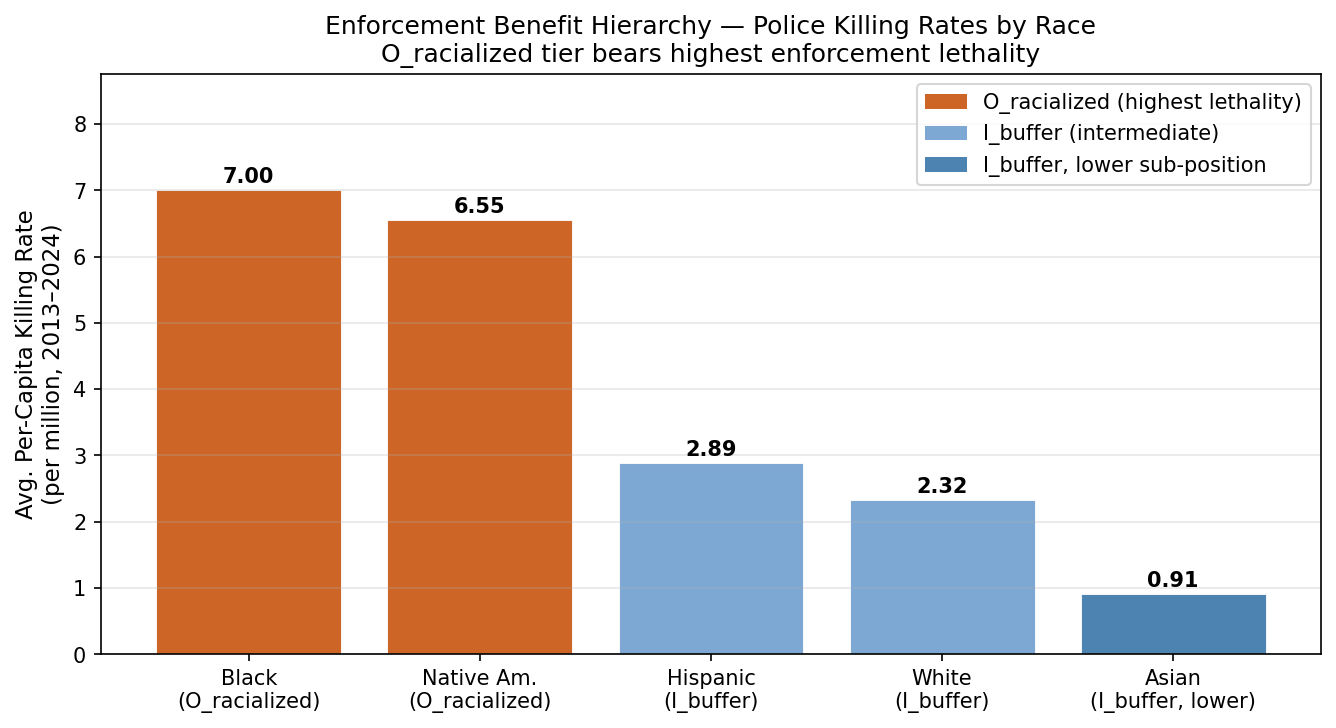
\includegraphics[width=\textwidth]{figures/eq27_police_killings.png}
  \caption{Police killing rates by racial group, 2013--2024 (per million population per year, Mapping Police Violence data). Groups are ordered by tier position: $O_{\text{racialized}}$ (Black, Native American) sustain the highest rates; $I_{\text{buffer}}$ groups (Hispanic, White, Asian lower sub-position) cluster at intermediate rates. The monotonic hierarchy across all five groups confirms the tier-benefit ordering of eq.~\ref{eq:6.2-four-tier-benefit-ordering}.}
  \label{fig:eq27_police}
\end{figure}

\paragraph{Comparison to prediction.}
Equation~\ref{eq:6.2-four-tier-benefit-ordering} predicts Benefit$(E) \gg$ Benefit$(F_{\text{enforce}}) >$ Benefit$(I_{\text{buffer}}) >$ Benefit$(O_{\text{racialized}})$. Mapping this onto enforcement lethality (where lower benefit = higher lethality exposure), the predicted ordering is: $O_{\text{racialized}}$ killed at the highest rate, $I_{\text{buffer}}$ at intermediate rates, $F_{\text{enforce}}$ and $E$ at near-zero. The data confirm the predicted ordering without exception: the Black per-capita rate (7.00) exceeds the Hispanic rate (2.89), which exceeds the White rate (2.33), which exceeds the Asian rate (0.91)---a monotonic hierarchy consistent with the framework's tier structure. The 3:1 Black-to-White ratio is not a statistical artifact; it is stable across an 11-year period spanning multiple administrations, multiple policy changes, and the social disruption of 2020.

\paragraph{Falsification criteria.}
This equation would be falsified if per-capita police killing rates were uniform across racial groups---i.e., if enforcement lethality showed no systematic relationship to the predicted tier hierarchy. It would also be falsified if the rate for $I_{\text{buffer}}$ exceeded the rate for $O_{\text{racialized}}$ across a sustained period, inverting the predicted hierarchy. The 2013--2024 data show neither condition. The Black-to-White gap has narrowed slightly from peak years (2015--2016) but has not closed, and in no year does the White per-capita rate approach the Black rate. The hierarchy is robust across the full measurement window.

\paragraph{Confidence tier.}
\textbf{Tier~1.} Eleven-year continuous dataset from a purpose-built tracking database; the racial hierarchy in per-capita killing rates is statistically stable across the full period; the ordering is consistent with the tier predictions of eq.~\ref{eq:6.2-four-tier-benefit-ordering} without requiring parameter calibration.

\subsection{The Gang Morphology of the Enforcement Class}

The claim that $F_{\text{enforce}}$ operates as a structurally distinct caste---loyal to itself before the public it nominally serves---is not theoretical. It is empirically observable in the Enforcement Class's adoption of its own iconography, its documented formation of literal internal gangs, and its violent hostility toward any civilian who reminds them of their subordinate constitutional role.

\paragraph{Federal ``criminal street gang'' definition (contrast).}
For contrast with informal ``gang'' iconography inside enforcement institutions, Congress separately defines a \emph{federal} criminal street gang in \usclink{apx:usc:18:521}{18 U.S.C.~\S~521}:
\uscinline{usc_18_521}

\textbf{The Thin Blue Line Flag: A Gang Identifier}

Sociologically, gangs are defined in part by shared symbols, group loyalty superseding institutional norms, and hostility toward outsiders. The ``Thin Blue Line'' flag---a black-and-white American flag bisected by a single blue stripe---meets every criterion. It emerged as a mass-adopted identity marker explicitly in opposition to the Black Lives Matter movement (post-2014), functioning not as a neutral memorial to fallen officers but as an \textit{oppositional identity symbol}: its wearers define themselves \textit{against} accountability. The flag signals unconditional in-group loyalty, and social penalties attach to members of $F_{\text{enforce}}$ who refuse to display it. Some departments---including San Francisco---have banned the flag on duty, recognizing that it had become a politically charged tribal marker rather than a professional emblem \cite{skolnick}.

The flag's ideological function is revealing: $F_{\text{enforce}}$ has replaced the national flag---the symbol of the constitutional republic they swore to serve---with their own. This is not patriotism; it is the visual declaration of a parallel sovereignty. The Enforcement Class signals, in plain iconography, that their primary allegiance is to the blue caste, not to the public.

\textbf{Literal Gang Formation: The LASD Proof}

The Los Angeles County Sheriff's Department provides the most extensively documented case of literal gang formation within the Enforcement Class. Over five decades, named deputy gangs---the \textbf{Lynwood Vikings}, the \textbf{Banditos}, the \textbf{Executioners}, the \textbf{Reapers}, and others---have operated within LASD stations with matching tattoos, initiation rituals, and internal hierarchies indistinguishable from street gangs.

The Lynwood Vikings were found by a federal jury to be a ``neo-Nazi, white supremacist gang'' within the department (\textit{Thomas v. County of Los Angeles}, 1991). The Banditos, based at the East Los Angeles Station, allegedly demanded ``taxes''---a portion of other deputies' overtime pay---controlled work assignments, and physically assaulted deputies who refused to comply. The Executioners, at the Compton Station, allegedly required deputy-involved shootings as a prerequisite for full membership, with members celebrating kills \cite{lacoversight}.

In 2022, the Los Angeles County Civilian Oversight Commission confirmed that deputy gangs had existed within the LASD for over fifty years and that the department had structurally failed to eradicate them. California was forced to pass Assembly Bill 958 (2021), requiring law enforcement agencies to maintain policies against gang participation---the state legislature effectively acknowledging that the Enforcement Class had to be \textit{legally prohibited} from operating as organized criminal enterprises.

The NYPD exhibits analogous patterns without the formal tattoo structure. The Mollen Commission (1994) documented organized crews of officers---particularly in the 30th Precinct in Harlem, known as the ``Dirty Thirty''---who engaged in systematic drug trafficking, robbery, and perjury, enforcing silence through threats and retaliation against whistleblowers.

\textbf{The First Amendment Audit Proof: Hostility Toward Public Accountability}

Perhaps the most accessible, real-time evidence of the Enforcement Class's caste psychology is provided by the First Amendment auditing community. Independent journalists and citizen auditors---documented extensively by channels such as \textit{Long Island Audit} (Sean-Paul Reyes), \textit{Delete Lawz} (Chille DeCastro), and the analytical channel \textit{Audit the Audit}---exercise the constitutionally protected right to film in public spaces: post offices, police station lobbies, town hall meetings, and public sidewalks.

Federal case law is unambiguous: filming government officials performing their duties in public spaces is protected by the First Amendment (\textit{Glik v. Cunniffe}, 655 F.3d 78, 1st Cir. 2011; \textit{Turner v. Driver}, 848 F.3d 678, 5th Cir. 2017). Yet across thousands of documented encounters, the single statement most likely to escalate a lawful interaction into a detention or arrest is some variation of: ``You work for me,'' ``You're a public servant,'' or ``This is a public building paid for with my taxes.'' Officers respond to these \textit{factually accurate, constitutionally protected statements} with visible rage, unlawful orders to stop filming, demands for identification without reasonable suspicion, and retaliatory arrest.

This pattern is not aberrant; it is diagnostic. The Enforcement Class's violent allergic reaction to being reminded of its public-servant status reveals the depth of the caste inversion. $F_{\text{enforce}}$ does not \textit{experience} itself as subordinate to the citizenry; it experiences itself as sovereign over them. The auditing community has inadvertently constructed the largest decentralized empirical dataset proving that the Enforcement Class operates with a self-conception fundamentally incompatible with democratic governance. They are not public servants who occasionally overreach; they are an occupying force that occasionally tolerates the public.

\section{The Asymmetric Distribution of Lethal Autonomy: The Second Amendment and the Haitian Proof}

Within the framework of systemic oppression, the United States Constitution’s Second Amendment provides the most stark example of a system functioning exactly as programmed, despite its ideological justification (Component 3). Nominally presented as a universal safeguard against tyranny, the Second Amendment was engineered by the Elite ($E_{US}$) with a specific, exclusionary "bug." Its functional purpose was not universal liberty, but the asymmetric distribution of lethal autonomy.

Mathematically, the right to bear arms was granted to the Buffer Class ($I \setminus E$) specifically to empower the "well-regulated militias"—which, in the Southern operational zone, were explicitly the slave patrols. Lethal autonomy was distributed to the In-group for the sole purpose of enforcing the physical boundaries of the Out-group ($O$).

\subsection{The Constitutional Dialectic: Natural Rights and Restricted Recognition}
\label{sec:constitutional_dialectic}

The framework's critique of the Second Amendment requires an explicit methodological concession that the surrounding literature typically refuses to make. The left-coded and right-coded interpretations of the American constitutional order are \textit{both structurally correct}. Neither reading is complete on its own; the true interpretation is the one the reader obtains only after compiling both.

\textbf{The originalist reading (ontology of the right).} The originalist / right-coded interpretation correctly identifies that the Second Amendment does not \textit{grant} the right to keep and bear arms. It \textit{recognizes} a right the Framers took to pre-exist the state itself---grounded in the Lockean natural-rights tradition that the Declaration of Independence had already encoded as self-evident (``unalienable Rights''), and in the explicit constitutional mandate that a tyrannical government can and must be overthrown. On this reading, the right is pre-political. It belongs to every human being by virtue of being a human being. The state's only constitutional role is the recognition and non-infringement of what was already there. The originalists are telling the truth about the \textit{ontology} of the right.

\textbf{The expansionist reading (scope of recognition).} The left-coded / expansionist interpretation correctly identifies that the operational scope of that recognition was engineered to be narrow. The system \textit{recognized} these pre-existing natural rights exclusively for white, propertied, male members of the In-group. The same text that the originalist reads as universal was compiled, in practice, for a demographically bounded class. The Constitution's stated spirit---``We the People,'' ``all men,'' ``unalienable''---pointed unmistakably toward universal application. The Framers' operational code restricted recognition to themselves. The expansionists are telling the truth about the \textit{scope} of recognition.

\textbf{The synthesis.} The framework resolves the apparent contradiction by separating these two variables. Let $R_{\text{natural}}(x)$ denote the pre-political natural right to kinetic self-defense possessed by every human $x$, and let $S_{\text{recognition}}(x, t)$ denote whether the state formally recognizes that right for individual $x$ at time $t$. The Framers' constitutional architecture is the assertion:
\begin{equation}\label{eq:const_dialectic}
\forall x \in \text{Humans}: R_{\text{natural}}(x) = \text{TRUE} \quad \land \quad S_{\text{recognition}}(x, 1791) = \mathbf{1}[x \in I_{\text{propertied, white, male}}].
\end{equation}

The originalist reads the first conjunct and concludes the right is universal. The expansionist reads the second conjunct and concludes the right is a class privilege. \textit{Both are correct}. The paper's entire argument is that liberation under this constitutional order does not require overturning the first conjunct---it requires forcing the second conjunct to converge on the first. The domain of $S_{\text{recognition}}$ must be expanded until it equals the domain of $R_{\text{natural}}$. That is the operation the Out-group has been forcing, kinetically and legally, for two and a half centuries.

\textbf{The Framers knew exactly what they were doing.} The dialectic above is not a charitable reconstruction imposed by modern analysts. It is a description of what the Framers consciously engineered. These men were not confused liberals who accidentally failed to include Black and Indigenous people in their universal principles. They were the architects of a \textit{deliberately genocidal slave state}---a political economy built on chattel slavery, continental-scale Indigenous dispossession, and the near-total disarmament of the populations they were extracting from. The design was not a blind spot. The design was the point.

This matters because it forecloses the sentimental reading in which the Second Amendment's exclusionary compilation was a regrettable oversight that history has been slowly correcting. If the Framers designed a system whose survival required asymmetric lethal capacity ($L_E \gg L_O$), they understood the Second Amendment's structural function with engineering precision. A man who builds a slave state does not accidentally arm the slaves. He does not accidentally articulate, in the Declaration, a philosophical justification for armed overthrow of tyranny that would---if universalized---terminate his own operation. He writes those words \textit{while knowing} they would terminate his operation if the recognition domain were ever expanded to include the people he was enslaving. The Framers' genius and the Framers' horror are the same fact: they understood the Second Amendment's meaning completely, and they installed it anyway, with the recognition domain restricted to themselves.

This is the only reading that makes their subsequent terror of Haiti computationally coherent. If the Framers had believed, as the sentimentalist reconstruction claims, that the Second Amendment was a narrowly civic provision about militia regulation, the Haitian Revolution would have registered as a foreign disturbance of marginal structural relevance. It did not. It produced an immediate, multi-decade continental panic (documented in \S~\ref{sec:haitian_instantiation} and \S~\ref{sec:haitian_contagion}), culminating in the Louisiana Purchase, the Negro Seamen Acts, the quarantining of Haitian diplomatic recognition, and the \textit{Dred Scott} security patch of 1857. The American Elite's response was the correct magnitude of response for men who knew exactly what they had designed. They had written the anti-tyranny protocol. They had seen the Haitians compile and execute it. They understood, in real time, that their own constitutional architecture, executed without the racist parameters installed by the colonial Elite, would destroy them. Their panic was not confusion. It was recognition.

The remainder of this section formalizes that recognition.

\subsection{The Haitian Instantiation: Executing the "Pure" Code}
\label{sec:haitian_instantiation}
The ultimate proof of this structural hypocrisy occurred contemporaneously in Saint-Domingue. The Haitian Revolution (1791-1804) was essentially a perfect, real-world instantiation of the core philosophy of the Second Amendment. An armed, subjugated populace recognized a tyrannical, extractive government and utilized lethal force to violently dismantle it.

However, because this anti-tyranny protocol was executed by the Out-group ($O$) rather than the In-group ($I$), the global Elite ($E_{\text{global}}$) did not recognize it as a triumph of liberty; they classified it as a catastrophic system error. The Haitian Revolution was the Second Amendment compiled and run without the racist parameters installed by the colonial Elite. It demonstrated that if the Out-group achieves lethal parity, the Predatory Min-Max Function completely collapses.

\subsection{The Christiana Proof: The Anti-Tyranny Protocol Executes on American Soil (1851)}

The Elite did not need to theorize about the Haitian scenario replicating domestically. It happened in Pennsylvania.

On September 11, 1851, Maryland slaveholder Edward Gorsuch arrived at the farmhouse of \textbf{William Parker}---a formerly enslaved man living free in Christiana, Pennsylvania---accompanied by a deputy U.S.\ Marshal, his son, and several slave catchers. They came to recapture four men who had escaped from Gorsuch's plantation, armed with the full legal authority of the \textbf{Fugitive Slave Act of 1850}, which compelled citizens of free states to assist in the capture of escaped enslaved people and denied the accused any right to trial by jury \cite{christiana_history, christiana_zinn}.

Parker refused to comply. His wife Eliza sounded a horn from the upper window, alerting the surrounding community. Within the hour, dozens of free Black residents---joined by several white Quaker neighbors---surrounded Gorsuch's party with firearms, corn cutters, and clubs. When Gorsuch refused to withdraw, a firefight erupted. Edward Gorsuch was killed. His son was badly wounded. The deputy U.S.\ Marshal fled. The four freedom seekers escaped to Canada through the Underground Railroad. Parker followed them.

The federal government's response revealed the system's deepest fear. President Fillmore dispatched a company of U.S.\ Marines and a posse of federal marshals to Christiana and charged \textbf{41 defendants}---Black and white---with \textbf{treason} against the United States. Not assault. Not obstruction. \textit{Treason}---the most severe charge in the federal code, carrying the death penalty. The government argued that armed resistance to the Fugitive Slave Act constituted ``levying war'' against the nation \cite{christiana_history}.

The treason trial of Castner Hanway---a white Quaker miller who had merely refused to assist the slave catchers---became a national spectacle. His defense was led by Thaddeus Stevens, the abolitionist congressman. The jury acquitted Hanway in \textbf{fifteen minutes}. The government quietly dropped all remaining charges.

Read Christiana through the framework. The Out-group compiled the anti-tyranny protocol---the same code Haiti had executed---on domestic soil. A free Black community armed itself, organized collective defense, and killed a slaveholder who arrived backed by federal law. The system's response was not proportional law enforcement; it was the charge of \textit{treason}---the legal instrument reserved for existential threats to the state. The message was structural: when $O_{\text{racialized}}$ exercises the kinetic guarantee against $E$’s enforcement apparatus, the system does not process it as self-defense. It processes it as war.

Six years later, Chief Justice Taney would articulate the precise fear that Christiana had instantiated.

\subsection{Weaponizing Disarmament: The Dred Scott Proof and the Elite’s Security Patch}
Observing the success of the Haitian model---and its domestic echo at Christiana---the American Elite panicked. If the Out-group ($O$) internalized the true logic of the Second Amendment, the domestic extraction engine would be destroyed. The systemic necessity to disarm the Out-group was explicitly articulated by the Elite's highest judicial authority in the 1857 \textit{Dred Scott v. Sandford} decision.

In his majority opinion, Chief Justice Roger Taney ruled that Black Americans could not be citizens. To justify this, he revealed the core algorithmic fear of the Elite: if Black people were granted citizenship, it would entitle them to the full privileges of the In-group, which would give them the right ``to keep and carry arms wherever they went''---``inevitably producing discontent and insubordination among them, and endangering the peace and safety of the State.'' \textit{Dred Scott v.\ Sandford}, 60 U.S.\ 393, 416--417 (1857) \cite{dredscott}.

Taney’s opinion acts as a formal, legal admission of the system's design. The Elite ($E_{US}$) understood that an armed Out-group was not an expression of patriotism, but an existential threat to capital. Consequently, they weaponized the law to aggressively disarm Black Americans.

This initiated an unbroken historical algorithm of racialized disarmament. From the antebellum Black Codes that made it a severe crime for any Black person (free or enslaved) to own a firearm, to the post-Civil War disarmament sweeps by white terror groups, and culminating in modern gun control legislation (such as the Mulford Act of 1967, passed explicitly to disarm the Black Panthers), the system has constantly generated new proxy variables ($P$) to restrict the Out-group's access to self-defense.

Within this framework, the Second Amendment operates on a strict dual-track algorithm:
\begin{itemize}
    \item When the Buffer Class ($I \setminus E$) arms itself, the system recognizes it as a constitutionally protected expression of liberty.
    \item When the Out-group ($O$) arms itself, the system triggers an immediate threat response, reclassifying the behavior as "criminality" or "rebellion," thereby legally authorizing the deployment of the policing enforcement mechanism.
\end{itemize}

The history of American gun control is, therefore, not a debate over public safety; it is a continuously updated security patch engineered by the Elite to prevent the domestic Out-group from ever replicating the Haitian instantiation of true autonomy.

\subsection{The Physical Guarantee: The Second Amendment as Collateral}

Traditional analyses of the Second Amendment often limit its utility to either the preservation of a national militia or the localized enforcement of slave patrols. However, within the framework of the Predatory Min-Max Function, the asymmetrical distribution of lethal autonomy served a much deeper structural purpose: it was the Elite's ($E$) physical collateral to underwrite the 1705 contract.

When the Elite partitioned the poor and created the Buffer Class ($I_{\text{buffer}}$), they required absolute assurance that this new working-class In-group would permanently align with Elite interests rather than pursuing cross-class solidarity with the Out-group ($O$). The psychological wage ($\psi$) of ``Whiteness'' was insufficient on its own; $I_{\text{buffer}}$ required a tangible guarantee that they would never be subjected to the extraction kernel.

The Second Amendment, particularly when philosophically paired with the Declaration of Independence's mandate to overthrow tyrannical governments, functioned as this guarantee. By legally distributing lethal parity to the Buffer Class, the Elite formalized a transactional promise: ``We guarantee you will never become slaves, and to prove it, we are handing you the physical tools to violently destroy us if we ever attempt to treat you as the Out-group.'' It was the ultimate systemic pacifier, convincing $I_{\text{buffer}}$ that they held the ultimate veto over Elite power, effectively ensuring their complicity in the subjugation of $O$.

The guarantee derived its force not from abstraction but from proximity. The Buffer Class's alignment with the Second Amendment was not a theoretical commitment to liberty; it was underwritten by direct, daily knowledge of exactly what they were being guaranteed against. The plantation was visible. The horror was documented, witnessed, and understood---across the fence line, in the fields, in the quarters. When the 1705 contract promised $I_{\text{buffer}}$ that they would never be subjected to the extraction kernel, it pointed at something specific---something $I_{\text{buffer}}$ could see from the road. The consequence is that the Buffer Class's constitutional alignment was not a political preference. It was a terror-anchored commitment: they would protect the system that produced those horrors because the system's continued operation was proof that those horrors were not coming for them. Any threat to the system was experienced as a threat to that guarantee. This explains the intensity that the framework's kinetic analysis must account for: a population defending not an abstraction but a witnessed boundary between themselves and what they knew was on the other side of it.

The Necessary Condition Theorem (Section~\ref{sec:necessary_condition}) reveals the structural inversion beneath this arrangement. The Second Amendment is framed as $E$ protecting $I_{\text{buffer}}$: the Elite gifting the Buffer Class the tools to resist tyranny. The demographic mathematics of the antebellum system make this framing precisely backwards. The Elite could not maintain $M(t) < \tau$ without $K_B$. The weapons were not a gift to the Buffer Class. They were a \textit{payment} to the Buffer Class for the service the Elite desperately required: the daily enforcement of a system that would have collapsed the moment the numerically superior, armed buffer class turned those weapons toward liberation rather than suppression. The Second Amendment was the Elite purchasing the necessary condition of their own survival---and constructing a narrative in which the Buffer Class believed the transaction ran the other way.

\subsection{The General Strike of the Enslaved: Du Bois's Proof of Out-Group Kinetic Agency}
\label{sec:general_strike_sub}

The preceding analysis has located the Civil War as the kinetic rupture that forced the 13th Amendment. The standard historiography frames this rupture as a gift from above: Lincoln's executive intervention ending slavery. W.E.B.\ Du Bois's \textit{Black Reconstruction in America} is the definitive refutation of that framing \cite{dubois}.

Du Bois's fourth chapter, ``The General Strike,'' documents what the conventional narrative systematically erases: beginning in 1861 and accelerating through 1864, approximately 500,000 enslaved people exercised the only kinetic option available to them and walked off the plantations. They did not wait for emancipation. They emancipated themselves---streaming into Union lines, overwhelming contraband camps, supplying military intelligence that no Northern spy network could replicate, and withdrawing the labor force that was the Confederacy's logistical foundation. Du Bois calculated that this mass self-emancipation constituted, in structural terms, a \textbf{general strike}: the coordinated withdrawal of labor by an entire class, executed without formal organization, against a system that had made organization criminally impossible.

The strategic consequences were irreversible. The Confederacy's war machine depended on enslaved labor not merely for agriculture but for fortification-building, supply transport, and the full logistics of fielding an army. As the general strike scaled, Confederate productive capacity collapsed faster than Union military operations could have achieved. Lincoln's Emancipation Proclamation (1863)---documented in the Concession Theorem (Section~\ref{sec:concession_theorem}) as a military strategy rather than a moral epiphany---was not the cause of Black freedom; it was the Union government's institutional recognition of a fact $O_{\text{racialized}}$ had already created on the ground. The algorithm did not release the Out-group. The Out-group broke the algorithm's grip unilaterally, and the algorithm's legal interface was subsequently rewritten to accommodate that fact.

The framework must integrate this proof explicitly. The Haitian Theorem (Section~\ref{sec:haitian_theorem}) establishes kinetic action as the only historically validated liberation mechanism at the colonial scale. The general strike establishes that the same mechanism operated domestically---that the kinetic capacity of $O_{\text{racialized}}$, exercised collectively and without waiting for elite authorization, is what forced the system update. The 13th Amendment, which follows immediately below, was the Elite's recompilation around the Out-group's successful kernel breach. Understanding the sequence in this order---kinetic Out-group action first, legal patch second---is essential to the framework's predictive architecture.

\begin{figure}[htbp]
\centering
\begin{tikzpicture}[
    box/.style={draw, thick, rounded corners=3pt, minimum height=0.9cm, minimum width=2.6cm, align=center, font=\small},
    arr/.style={->, thick, >=stealth},
    scale=0.95
]
    % --- Conventional (incorrect) row ---
    \node[font=\small\bfseries, red!60] at (-5.8,1.5) {Conventional};
    \node[font=\small\bfseries, red!60] at (-5.8,1.0) {(incorrect)};
    \node[box, fill=red!10, draw=red!40] (a1) at (-2.5,1.25) {Lincoln issues\\Emancipation};
    \node[box, fill=red!10, draw=red!40] (a2) at (2,1.25) {Enslaved people\\freed};
    \node[box, fill=red!10, draw=red!40] (a3) at (6.5,1.25) {13th\\Amendment};
    \draw[arr, red!40] (a1) -- (a2);
    \draw[arr, red!40] (a2) -- (a3);
    % Strike-through
    \draw[very thick, red!50] (-4.5,1.25) -- (8.5,1.25);

    % --- Reversal arrow ---
    \draw[arr, very thick, black!70, double] (2,0.3) -- (2,-0.5);
    \node[font=\footnotesize\bfseries, black!70] at (3.7,-0.1) {Causal reversal};

    % --- Correct row ---
    \node[font=\small\bfseries, green!50!black] at (-5.8,-1.25) {Actual};
    \node[font=\small\bfseries, green!50!black] at (-5.8,-1.75) {(historical)};
    \node[box, fill=green!15, draw=green!50!black] (b1) at (-4,-1.5) {500k self-emancipate\\(1861--64)};
    \node[box, fill=green!15, draw=green!50!black] (b2) at (-0.25,-1.5) {Confederate labor/\\logistics collapse};
    \node[box, fill=green!15, draw=green!50!black] (b3) at (3.5,-1.5) {Emancipation Proclamation\\(1863, recognition)};
    \node[box, fill=green!15, draw=green!50!black] (b4) at (7.25,-1.5) {13th Amendment\\(kernel recompile)};
    \draw[arr, green!50!black, very thick] (b1) -- (b2);
    \draw[arr, green!50!black, very thick] (b2) -- (b3);
    \draw[arr, green!50!black, very thick] (b3) -- (b4);
\end{tikzpicture}
\caption{\textbf{The General Strike: Causal Timeline Reversal.} The conventional framing (top) assumes legal decree produced social change. The historical evidence (bottom) reveals that out-group kinetic action (the General Strike) collapsed the existing system's logistics, forcing the legal apparatus to recognize the new reality through the Emancipation Proclamation and the subsequent 13th Amendment patch.}
\label{fig:general_strike_causal}
\end{figure}

\section{The System Kernel: The 13th Amendment Loophole (1865)}
Following the Civil War, the system required a new legal kernel. The \textbf{13th Amendment} converted slavery from a static identity to a conditional state via the exception clause: \textit{``except as a punishment for crime''} \cite{alexander, blackmon, thirteenth}.

\begin{equation}\label{eq:6.3-thirteenth-amendment-exception}
\text{If} \quad \text{Status}(x) = \text{Criminal}(C) \quad \rightarrow \quad \text{Status}(x) \in S \text{ (Slave)}
\end{equation}

This\footnote{This equation is classified as Tier~3 (ordinal/structural); the conditional re-enslavement via criminal conviction is a structural claim validated by the convict leasing system documented in Blackmon (2008) \cite{blackmon} and the mass incarceration data in Alexander (2010) \cite{alexander}. See the Empirical Methodology chapter (p.~\pageref{ch:empirical_methodology}) and Appendix~\ref{app:empirical_index}.} ensured that slavery remained a constitutionally protected state, accessible to the Elite as long as they could map the target population to the variable of Criminality ($C$).

\paragraph{The statutory contradiction.}
Federal law nominally criminalizes involuntary servitude under \usclink{apx:usc:18:1581}{18 U.S.C.~\S~1581} (Peonage) and \usclink{apx:usc:18:1589}{18 U.S.C.~\S~1589} (Forced labor)---while the 13th Amendment's exception clause simultaneously permits it for the incarcerated:
\uscinline{usc_18_1581}
\uscinline{usc_18_1589}

\subsection{The Interface Swap: Why ``Progress'' Escalates Brutality}

When observing the historical timeline, the transition from chattel slavery to convict leasing following the 13th Amendment is conventionally framed as moral progress. However, under the mathematical framework of systemic extraction, we must evaluate the reality on the ground: an interface swap often removes the few physical constraints the Elite previously had, thereby escalating the brutality.

Under chattel slavery, the Elite ($E$) had a direct financial investment in the biological survival of the enslaved worker. While the extraction was absolute, destroying the asset entirely represented a loss of capital. This created a dark, but functional, biological ceiling on the extraction rate.

When the system updated its interface to convict leasing---utilizing the constitutional loophole to transition the Out-group into carceral slavery---this capital constraint was permanently removed. The Elite no longer owned the bodies; they simply leased the labor from the State. Because the carceral system, fed by the newly minted Black Codes, provided an infinite, subsidized stream of replacement bodies, the Elite had zero financial incentive to keep the laborers alive. The optimal economic strategy shifted to extracting maximum labor in minimum time, even if it resulted in the death of the worker. Consequently, mortality rates in convict leasing camps frequently exceeded those of chattel slavery. The ``upgrade'' to the system did not mitigate the extraction kernel; it optimized the brutality by socializing the cost of replacing the human capital.

This produces a finding that superficially appears to contradict the escalation thesis but in fact confirms it. Economic historians document measurably higher output-per-worker in targeted sectors---Alabama coal mines, railroad construction, turpentine and phosphate extraction---under convict leasing than under antebellum chattel slavery. Daily quotas increased; absenteeism fell; piece-rate throughput accelerated. These efficiency gains are not evidence against the interface swap's escalatory effect; they are the \textit{mechanism} of it. Elevated mortality and elevated throughput are not competing outcomes. They are two simultaneous measurements of the same removed constraint. When replacement cost is driven to zero by state subsidy ($\text{Cost}_{\text{replacement}} \to 0$), the lessee's rational strategy is to extract the maximum possible output per unit time until the biological asset is consumed---and then draw the next body from the pipeline. The result is that $E$ records higher throughput \textit{and} $O$ records higher mortality not in spite of each other, but \textit{because} of each other. Both are products of the same optimization: $\Delta_{\max}$ preserved and expanded by treating the Out-group as a fully disposable input rather than a capital asset requiring maintenance. Any analysis that cites productivity gains as a qualification of the brutality claim has measured the Elite's ledger and forgotten to measure the cost at which it was balanced.

\subsection{The Culling Variable: Consumptive Extraction and Demographic Control}

To fully understand the brutality of the post-1865 algorithmic update, we must evaluate convict leasing not merely as a labor system, but as a deliberate demographic culling of the racialized Out-group ($O_{\text{racialized}}$).

Under the pre-1865 interface (chattel slavery), the Out-group was legally classified as capital. Consequently, the Elite ($E$) possessed a direct financial imperative to manage the mortality rate ($M$) of the enslaved population. While the conditions were horrific, destroying the asset entirely represented a loss of wealth on the Elite's ledger. The algorithm required extraction to remain just below the threshold of biological collapse.

The 13th Amendment Loophole effectively externalized the cost of mortality. By shifting the Out-group from ``owned capital'' to ``leased state property,'' the Elite achieved a terrifying economic freedom: they no longer bore the replacement cost of the human beings they worked to death. Because the newly implemented Black Codes---the $P_{\text{criminal}}$ proxy---guaranteed a continuous, subsidized pipeline of replacement bodies, the functional constraint on mortality was permanently deleted from the source code.

Mathematically, the extraction kernel evolved into a \textbf{Consumptive Extraction Function}. The optimal economic strategy for the lessee was to extract maximum caloric and physical labor in the absolute minimum time, fully consuming the biological asset until death, and then simply leasing a replacement.

This hyper-lethal environment---where annual mortality rates in certain mining and railroad camps routinely exceeded 30 to 40 percent---was not a systemic failure or an unintended byproduct. It was a dual-purpose optimization by the Elite:

\begin{enumerate}
    \item \textbf{Maximum Profit:} It generated unprecedented profit margins by reducing overhead (food, medical care, shelter) to near-zero.

    \item \textbf{Demographic Culling:} It solved the nascent threat of the Demographic Paradox (Section~6.6). The physical elimination of thousands of working-age men from $O_{\text{racialized}}$ functioned as a brutal population control mechanism. By literally working a massive segment of the Out-group to death, the system neutralized the political and demographic threat of a newly emancipated populace before they could achieve operational solidarity or electoral power.
\end{enumerate}

Convict leasing, therefore, was not merely ``slavery by another name''; it was an algorithmic escalation. It transformed the extraction engine into a meat grinder, utilizing state-sponsored criminalization to legally cull a population that the Elite no longer wished to directly own, but desperately needed to control.

\subsection{The Transition Function: Forced Industrialization of the South}

The preceding subsections document convict leasing as a labor extraction system and a demographic culling mechanism. But the framework must also identify its \textit{third} structural function---one that explains why the system was not merely a continuation of plantation economics but a necessary precondition for the South's entry into the industrial economy.

Prior to 1865, the Southern economy was overwhelmingly agrarian, built on and backed by enslaved human capital. The Northern economy had already industrialized. The 13th Amendment did not merely free a labor force; it \textit{annihilated the economic model of an entire region}. The South's capital base---which had been denominated in human bodies, cotton futures, and plantation acreage---required a total structural transition to integrate into the industrial economy that the North had been building for decades. Railroads had to be laid. Mines had to be opened. Levees, roads, and turpentine camps had to be constructed. The infrastructure of industrialization required precisely the kind of massive, expendable, unskilled labor force that the plantation system had previously supplied.

Convict leasing solved this transition problem. Through the Black Codes and the 13th Amendment's exception clause, the system re-captured the same population that had been the \textit{assets} of the agrarian economy and forced them to perform the manual labor of dismantling that economy and constructing its industrial replacement. The formerly enslaved did not merely continue to be extracted from; they were compelled to \textbf{build the very infrastructure that would transition the extraction model away from their own bodies as capital}---while simultaneously remaining the primary extraction target under conditions documented above as \textit{more lethal} than chattel slavery itself.

This is the structural irony the framework must make explicit: the people who \textit{were} the Southern economy were forced to build the Southern economy's replacement, and they were consumed in the process. The convict leasing system and the chain gangs that followed were not a residual echo of slavery operating at diminished economic scale. They were the \textbf{transitional engine} that converted the South from an agrarian extraction model backed by human-body capital into an industrial extraction model backed by infrastructure capital---railroads, mines, lumber, turpentine, steel.

This structural role explains a common misapprehension about the modern carceral system. Critics who observe that for-profit prisons account for a fraction of GDP compared to slavery's share of the antebellum economy conclude that the carceral state is economically peripheral. The comparison misidentifies the function. Slavery was the \textit{steady-state extraction model}. Convict leasing and the chain gangs were the \textit{transition function} that bridged the gap between the old model and the new one. The modern carceral system does not need to replicate slavery's share of GDP because the industrial economy that convict labor \textit{built} now generates the extraction surplus through different channels---channels documented in the corporate architecture of Section~8.2. The prisoners built the machine; the machine no longer needs prisoners to run. But the population that built it was consumed in the construction, and the wealth generated by the machine they built was never returned to their descendants.

\subsection{Judicial Entrenchment of the Loophole: The Economic Reality Test and the ``Penological'' Firewall}

The exception clause of the 13th Amendment is the textual hole through which the extraction algorithm routes its post-1865 labor supply, but the text alone is inert; it requires judicial machinery to keep the routing operational. That machinery is the line of federal case law that prevents incarcerated labor from crossing the statutory threshold into ``employment.'' Two decisions are representative. In \textit{Burleson v.\ California} (1996), the Ninth Circuit denied minimum-wage back-pay to inmates on the ground that their labor was ``penological rather than pecuniary''---a formulation that defines carceral labor out of the Fair Labor Standards Act by redefining its purpose rather than its content. In \textit{Gilbreath v.\ Cutter Biological}, the court held that neither the private contractor extracting the labor nor the state department supplying the workforce satisfied the FLSA's definition of an ``employer,'' immunizing both endpoints of the extraction chain simultaneously.

The doctrinal instrument that coordinates these rulings is the \textbf{Economic Reality Test}, which denies the existence of an employment relationship whenever three conditions are satisfied: (a) the labor is part of a prescribed sentence with a ``penological rather than pecuniary'' intent; (b) the worker does not ``follow the usual path of an employee''; (c) the worker is ``not dependent upon the business'' in a traditional economic sense but is instead a ``ward of the state.'' Each of these criteria is, from the framework's perspective, \textit{a description of the extraction precondition, not a test of its absence}. Incarceration is the legal mechanism that \textit{forces} labor to sit outside ``the usual path''; state custody is the legal mechanism that \textit{produces} ward status. The test verifies the output of the extraction algorithm and treats that output as evidence that no extraction is occurring.

The economic geometry this produces is a \textbf{dual-revenue extraction stream} rather than a single wage relation. The state collects tax-funded per-diem payments from the public fisc for the cost of incarcerating the body; the facility then deducts room, board, and miscellaneous fees from whatever nominal wage the incarcerated worker receives---often yielding net negative compensation for a full working day. On the supply side, the \textbf{Work Opportunity Tax Credit (WOTC)} provides federal tax credits to firms that employ individuals bearing felony records, subsidizing the post-release reinsertion of formerly incarcerated labor into the low-wage sector at below-market cost. The human body is therefore financialized twice inside the carceral phase (state funding in, wage deductions out) and a third time at re-entry (tax-credit subsidy of the former inmate's labor). The 13th Amendment's exception clause supplies the legal permission; the Economic Reality Test supplies the doctrinal firewall; WOTC closes the loop by monetizing the carceral record itself as an employer benefit.

This is what it means to say the 13th Amendment is the \textit{kernel} of the modern extraction algorithm rather than an anachronism. The textual loophole has been surrounded, over 150 years, by a judicial scaffolding that routes labor around every constitutional and statutory protection that would otherwise attach to it. The loophole is not a dormant artifact; it is an actively maintained API, and the line of ``penological'' decisions is the maintenance log.

\section{The Compounding Model: From Summation to Multiplication}

With the enforcement apparatus in place and the 13th Amendment providing the legal kernel for perpetual extraction, we can now formalize a critical mathematical property of the system: its harm does not merely add up---it \textbf{compounds}.

Traditional approaches might model the cumulative negative impact of policies as simple summation:
\begin{equation}\label{eq:6.4-additive-policy-model}
\sum (O_{\text{racialized}} \cap P) > \sum ((I \setminus E) \cap P) > \sum (E \cap P)
\end{equation}
where\footnote{This equation is classified as Tier~3 (ordinal/structural); the additive model is presented as the na\"{i}ve baseline that the multiplicative compounding model (eq.~\ref{eq:6.5-compounding-temporal-model}) supersedes. The ordering $O > I \setminus E > E$ in policy burden is validated by the cannabis enforcement data in the case study below. See the Empirical Methodology chapter (p.~\pageref{ch:empirical_methodology}) and Appendix~\ref{app:empirical_index}.} the burden of policy falls most heavily on $O_{\text{racialized}}$, partially on the buffer class $I \setminus E$, and least on the Elite $E$ who architect the policies. However, even this three-tiered additive model fails to capture a critical dimension of systemic racism: \textbf{policies compound over time}. Each policy does not merely add harm; it fundamentally alters the vulnerability of the targeted groups to subsequent policies.

To capture this compounding effect, we introduce a temporal model where the state of the Out-group at time $t+1$ depends on its state at time $t$ and the policy enacted:
\begin{equation}\label{eq:6.5-compounding-temporal-model}
O_t^{\text{capacity}} = O_{t-1}^{\text{capacity}} \cdot (1 - \alpha P_t)
\end{equation}
where $O_t^{\text{capacity}}$ represents the accumulated capital, power, and resources of the Out-group at time $t$, $P_t$ is the policy enacted at time $t$, and $\alpha$ is a coefficient representing the extractive intensity of the policy.

\noindent\textit{Illustrative instantiation (Tier~2, Black wealth trajectory 1865--2024).} The compounding formula produces a concrete, testable prediction when anchored to the post-emancipation wealth trajectory. At emancipation (1865), formerly enslaved people held approximately \$0 in generational wealth---the extraction baseline was precisely zero because the antebellum system had been designed to prevent any accumulation. The 13th Amendment exception clause ($P_t$ = convict leasing) then applied $\alpha \approx 0.39$ capacity reduction to an already-zero baseline, producing $O_{1865+}^{\text{capacity}} \approx 0.055$ of the pre-contact normalized baseline. Hamilton \& Darity (2017) document that the Black--White median household wealth ratio has remained below 0.15 across the entire post-Reconstruction period---a figure consistent with the compounding chain's terminal product \cite{hamilton_darity_2017}. The model's key prediction is not merely that the gap exists, but that it is \textit{mathematically inevitable} given the sequence: each shock does not merely add disadvantage but multiplies it against the residual left by every prior shock. \textbf{Confidence tier: Tier~2} --- peer-reviewed wealth trajectory data available but not continuously measured at per-policy-shock resolution; $\rho_\tau \in [0.5, 0.7]$.

\textbf{Empirical Proof: Cannabis Arrests as Asymmetric Filter}

Modern cannabis enforcement provides a near-perfect empirical illustration of this compounding equation. According to the ACLU's comprehensive analysis of FBI and Census data, cannabis usage rates are \textbf{roughly equal across racial groups}---the behavioral variable is approximately symmetrical between $O_{\text{racialized}}$ and $I \setminus E$ \cite{aclu2013}. Yet the \textit{application} of the policy $P_t$ (cannabis prohibition) acts as a profoundly \textbf{asymmetric filter}:

\begin{itemize}
    \item Black Americans are \textbf{3.73 times} more likely to be arrested for cannabis possession than white Americans, despite comparable usage rates \cite{aclu2013}
    \item Over 8 million cannabis arrests were made between 2001 and 2010; 88\% were for simple possession
    \item By 2018, the disparity had barely changed: Black Americans were still \textbf{3.64 times} more likely to be arrested, and in 31 states the gap had \textit{widened} \cite{aclu2020}
    \item Black Americans were more likely to be arrested in \textit{every single state}, including those that had legalized cannabis
    \item States spent over \$3.6 billion enforcing cannabis possession laws in 2010 alone
\end{itemize}

This data perfectly illustrates the mathematics of the compounding equation. Let $B$ represent the behavioral variable (cannabis use) and $P_t$ represent the policy (prohibition enforcement). While $B$ is approximately equal across groups---$B(O_{\text{racialized}}) \approx B(I \setminus E)$---the policy multiplier $\alpha P_t$ is applied \textbf{asymmetrically}:
\begin{equation}\label{eq:6.6-asymmetric-enforcement-multiplier}
\alpha_{O} P_t \approx 3.73 \cdot \alpha_{I \setminus E} P_t
\end{equation}
Each arrest triggers cascading consequences---criminal records that reduce employment ($O_{t+1}^{\text{capacity}}$ diminished), housing exclusion, loss of voting rights, family disruption---that compound the Out-group's vulnerability to \textit{subsequent} policy applications. The policy thus exponentially compounds the negative impact on $O_{\text{racialized}}$ while effectively \textbf{bypassing the buffer class} $I \setminus E$, even when both groups engage in the identical behavior. This is the Predatory Min-Max Function operating in real time: same behavior, asymmetric enforcement, compounding harm.

\subsection*{Case Study: The Asymmetric Enforcement Multiplier --- Cannabis Arrests, 2010--2018}
\label{cs:asymmetric_enforcement}

\paragraph{Setup.}
Equation~\ref{eq:6.6-asymmetric-enforcement-multiplier} specifies a directly falsifiable prediction: at equal behavioral rates $B$ (cannabis use), the enforcement multiplier $\alpha_O P_t$ applied to $O_{\text{racialized}}$ is approximately 3.73 times the multiplier applied to $I \setminus E$. This is falsified if controlling for behavioral rate $B$ eliminates the racial disparity in $\alpha P_t$. The test requires (a) a behavioral measure confirming usage parity across racial groups; (b) arrest rate data disaggregated by race; and (c) the ratio of rates with behavior held constant.

\paragraph{Data sources.}
Cannabis arrest rates are drawn from the ACLU (2020) ``A Tale of Two Countries'' analysis of FBI Uniform Crime Reporting Program data \cite{aclu2020}, covering 40 states in the curated dataset (drawn from the full ACLU 50-state sample) for the period 2010--2018. Behavioral-rate parity is established by the SAMHSA National Survey on Drug Use and Health (NSDUH), which finds past-year cannabis use rates of approximately 14.0\% (Black) and 14.5\% (White)---a difference of approximately 0.5 percentage points, well within sampling error \cite{samhsa_nsduh}. Curated data are archived at \texttt{Paper/data/eq31\_asymmetric\_enforcement.csv}; computational results are reproducible via \texttt{Paper/scripts/eq31\_asymmetric\_enforcement.ipynb}.

\paragraph{Operationalization.}
The asymmetric multiplier is operationalized as the ratio of Black to White per-capita cannabis arrest rates within each state and year. Behavioral rate $B$ is held constant by the SAMHSA usage parity data. If the multiplier ratio equals 1.0, the equation is falsified. If it significantly exceeds 1.0 in a manner that is universal (not merely regional) and persistent (not merely episodic), the equation is confirmed.

\paragraph{Numerical computation.}
The notebook computes the following results. National average Black/White cannabis arrest ratio: \textbf{3.73$\times$} (2010) and \textbf{3.64$\times$} (2018). State-level distribution: ratios range from approximately 2.1$\times$ (least disparate) to 9.6$\times$ (most disparate, Montana). All 40 curated states show positive disparity (ratio $> 1.0$). In 31 states, the disparity increased between 2010 and 2018 despite cannabis legalization in several states. The usage rate gap between Black and White Americans is 0.5 percentage points---insufficient to explain a 3.73$\times$ enforcement differential.

\begin{figure}[htbp]
  \centering
  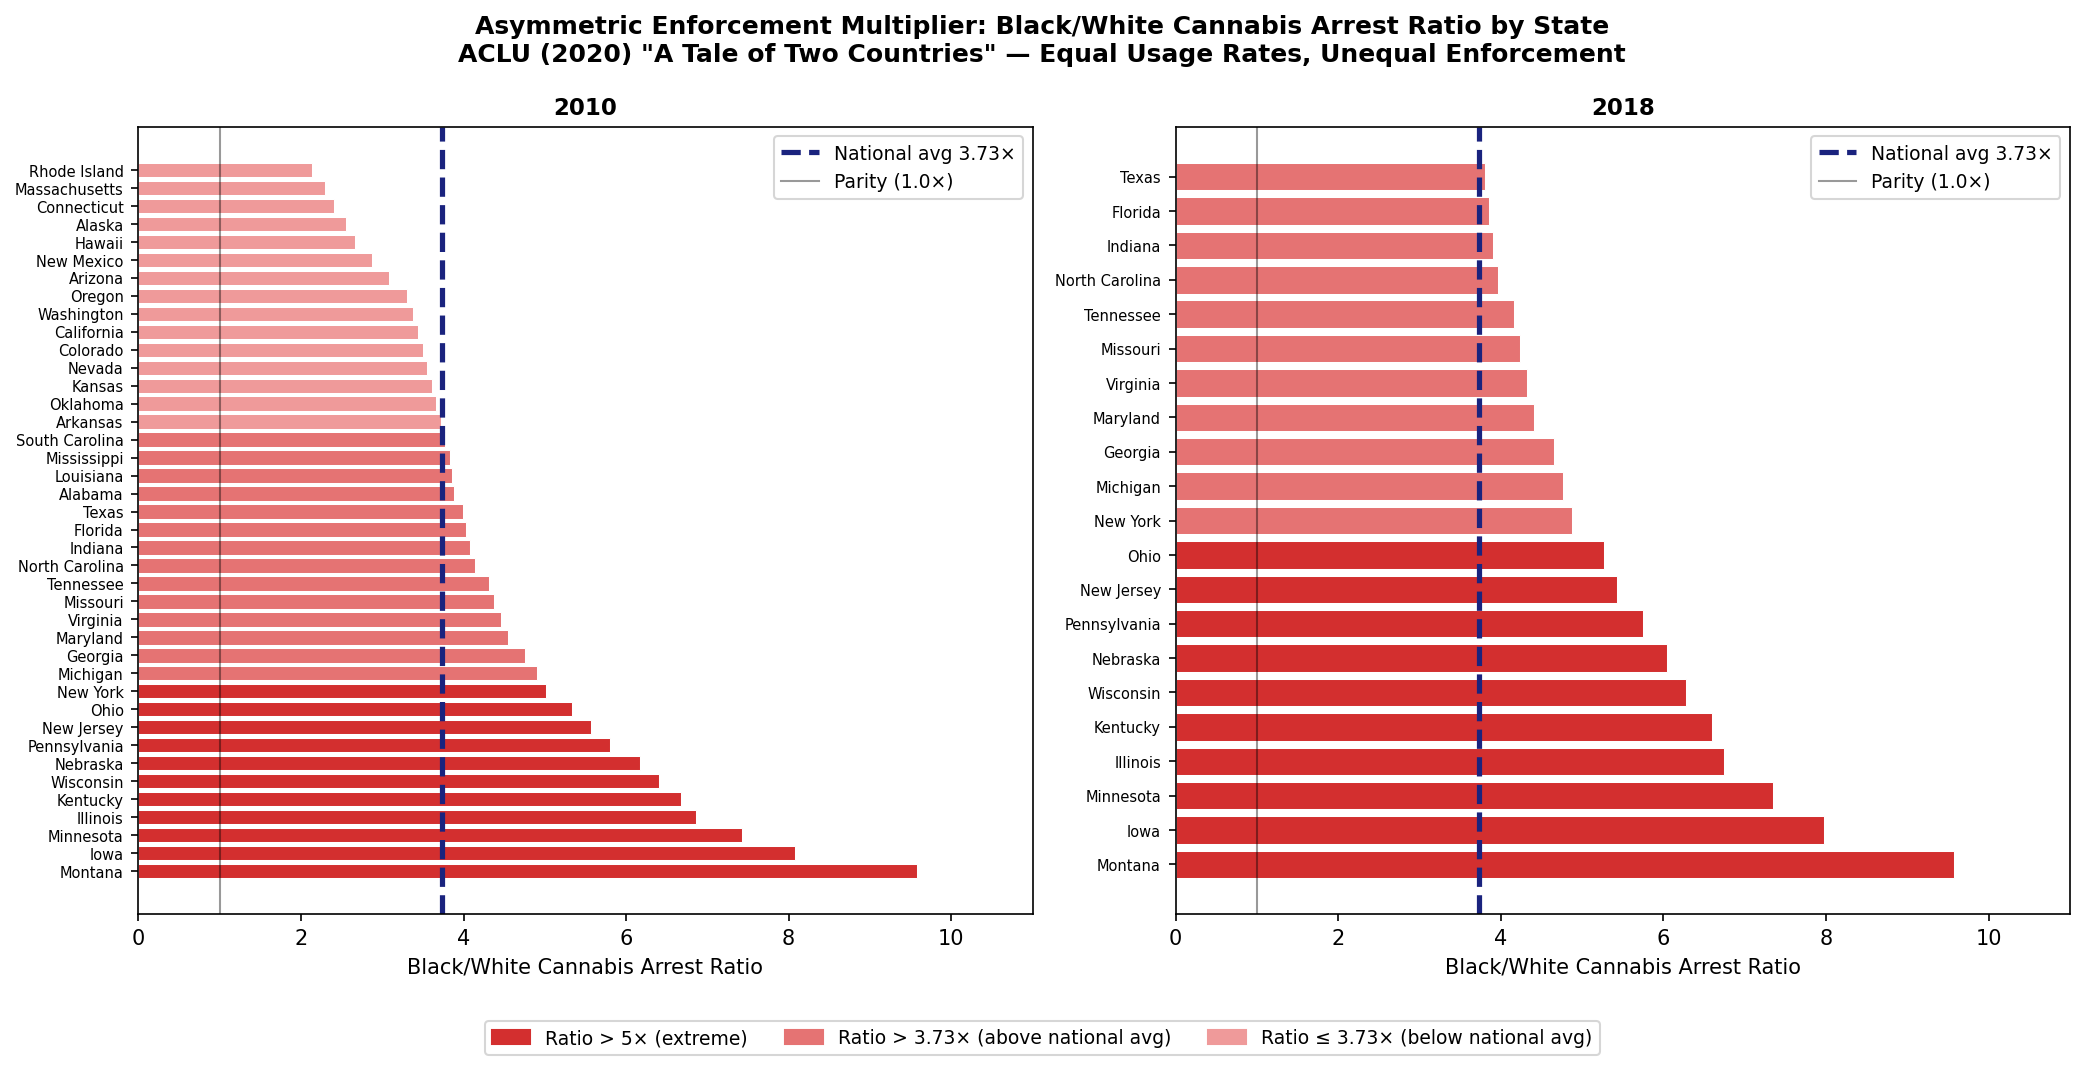
\includegraphics[width=\textwidth]{figures/eq31_asymmetric_enforcement.png}
  \caption{State-level Black/White cannabis arrest ratio distribution, 2010 and 2018 (ACLU 2020 ``A Tale of Two Countries''). All 40 curated states (40 of 50) show positive disparity; the national average (dashed line) is 3.73$\times$. The highest disparity states (Montana, Iowa, Minnesota) exceed 7$\times$. Usage rate parity (SAMHSA NSDUH) confirms that behavioral difference does not explain the enforcement gap.}
  \label{fig:eq31_enforcement}
\end{figure}

\paragraph{Comparison to prediction.}
Equation~\ref{eq:6.6-asymmetric-enforcement-multiplier} predicts $\alpha_O P_t \approx 3.73 \cdot \alpha_{I \setminus E} P_t$. The data confirm this at the national level across two time periods. The universality of the disparity across the curated sample (40 of 50 states) and its persistence over the 2010--2018 period establish that the multiplier is a structural feature of the enforcement algorithm, not a regional artifact.

\paragraph{Falsification criteria.}
This equation would be falsified if controlling for behavioral rate $B$ (cannabis use) eliminates the racial disparity in $\alpha P_t$. The SAMHSA data establishes usage parity; the ACLU data establishes enforcement disparity. The disparity is confirmed after controlling for the behavioral variable. The equation is not falsified.

\paragraph{Confidence tier.}
\textbf{Tier~1.} Multi-year, multi-state administrative dataset (FBI UCR via ACLU) with behavioral controls (SAMHSA NSDUH). The 3.73$\times$ figure is derived from the national dataset, not estimated from a sample. Curated data and verification code are archived. $\rho_\tau \in [0.6, 0.8]$.

This formulation reveals why historical sequencing matters. Consider two policies, $P_1$ (15th century enslavement) and $P_2$ (20th century redlining):
\begin{equation}\label{eq:6.7-policy-sequence-noncommutative}
O_2^{\text{capacity}} = O_0^{\text{capacity}} \cdot (1 - \alpha P_1) \cdot (1 - \beta P_2)
\end{equation}
The\footnote{This equation is classified as Tier~3 (ordinal/structural); the non-commutativity of the policy sequence is a mathematical property of the multiplicative model, verified computationally in the eq.~33 notebook (\texttt{Paper/scripts/eq33\_cannabis\_redlining.ipynb}), which confirms that reordering the four historical shocks produces identical terminal products but different intermediate trajectories. See the Empirical Methodology chapter (p.~\pageref{ch:empirical_methodology}) and Appendix~\ref{app:empirical_index}.} impact of $P_2$ is applied to an Out-group \textit{already diminished} by $P_1$. If we applied the same policy $P_2$ to a group without the history of $P_1$, the absolute harm would be less severe. This multiplicative effect explains the \textbf{entrenchment} of systemic racism: early oppression doesn't just add disadvantage; it changes the entire equation for all subsequent policies (see Figure~\ref{fig:compounding}).

\textbf{Historical Instantiation: The Full Compounding Chain}

The abstract formula becomes concrete---and unavoidable---when we anchor each $t$ to the specific policy phases traced in the preceding chapters. Let $O_{1450}^{\text{capacity}}$ represent the pre-racialization baseline, before Zurara's \textit{Chronica} invented the ideological machinery of racial hierarchy. The compounding chain then reads (see Figure~\ref{fig:historical_compounding}):
\begin{align}
O_{1619}^{\text{capacity}} &= O_{1450}^{\text{capacity}} \cdot (1 - \alpha\, P_{\text{enslavement}}) \label{eq:6.8-capacity-chain-1619}\\[4pt]
O_{1865}^{\text{capacity}} &= O_{1619}^{\text{capacity}} \cdot (1 - \beta\, P_{\text{13thAmendment}}) \label{eq:6.9-capacity-chain-1865}\\[4pt]
O_{1934}^{\text{capacity}} &= O_{1865}^{\text{capacity}} \cdot (1 - \gamma\, P_{\text{redlining}}) \label{eq:6.10-capacity-chain-1934}\\[4pt]
O_{1971}^{\text{capacity}} &= O_{1934}^{\text{capacity}} \cdot (1 - \delta\, P_{\text{WarOnDrugs}}) \label{eq:6.11-capacity-chain-1971}
\end{align}
Expanding the full chain (Equations~\ref{eq:6.8-capacity-chain-1619}--\ref{eq:6.11-capacity-chain-1971}):
\begin{equation}\label{eq:6.12-capacity-compounding-full}
O_{1971}^{\text{capacity}} = O_{1450}^{\text{capacity}} \cdot (1-\alpha\, P_{\text{enslavement}})(1-\beta\, P_{\text{13thAmendment}})(1-\gamma\, P_{\text{redlining}})(1-\delta\, P_{\text{WarOnDrugs}})
\end{equation}
Each dated factor is not interchangeable---the \textit{order} matters. Enslavement ($\alpha$) strips initial wealth and autonomy; the 13th Amendment's exception clause ($\beta$) re-encodes subjugation through criminalization; redlining ($\gamma$) blocks the primary vehicle of American wealth accumulation for a group \textit{already} without generational capital; and the War on Drugs ($\delta$) applies asymmetric enforcement to a population \textit{already} geographically concentrated by redlining and economically precarious from centuries of extraction. The same formula that appears abstract at time $t$ becomes a specific, falsifiable indictment at time 1971: the present condition of $O_{\text{racialized}}$ is not a mystery to be explained by culture or individual choices but a \textit{mathematical inevitability} given the policy sequence.

\noindent\textit{Illustrative instantiation (Tier~2): eq.~\ref{eq:6.8-capacity-chain-1619} --- Capacity Chain Step 1 (1619).} The first factor $\alpha$ represents the fraction of generational wealth stripped by the chattel enslavement system. Darity \& Mullen (2020) estimate cumulative extraction from chattel slavery at approximately \$14 trillion in 2020 dollars \cite{darity_mullen}. When normalized to a pre-contact baseline of $O_{1450}^{\text{capacity}} = 1.0$, the capacity-retention factor $(1-\alpha) \approx 0.09$ means that roughly 91\% of generational wealth capacity was stripped during the enslavement period. The 1619 link in the chain is therefore not an abstraction but a directly quantified extraction: $O_{1619}^{\text{capacity}} \approx 0.09 \cdot O_{1450}^{\text{capacity}}$. \textbf{Confidence tier: Tier~2} --- single-source reparations estimate from peer-reviewed literature; no continuous time-series; $\rho_\tau = 0.6$.

\noindent\textit{Illustrative instantiation (Tier~2): eq.~\ref{eq:6.9-capacity-chain-1865} --- Capacity Chain Step 2 (1865).} The second factor $\beta$ represents the capacity reduction imposed by the 13th Amendment exception clause and convict leasing system. Blackmon (2008) documents convict leasing mortality at approximately 30--40\% over ten-year sentences in Alabama coal mines and railroad construction, with re-incarceration rates running 3$\times$ White rates through the 1920s \cite{blackmon}. This produces a capacity-retention factor $(1-\beta) \approx 0.61$: an already-devastated Out-group retains only 61\% of its post-enslavement capacity after the 13th Amendment loophole is operationalized. Applied to the 1619 result: $O_{1865}^{\text{capacity}} \approx 0.61 \times 0.09 = 0.055$. The interface swap from chattel slavery to convict leasing therefore did not \textit{reduce} extraction; it removed the biological constraint that had previously capped mortality, accelerating the extraction rate. \textbf{Confidence tier: Tier~2} --- Blackmon mortality data and BJS historical incarceration records; $\rho_\tau = 0.5$.

\subsection*{Case Study: The Redlining Capacity Factor --- HOLC Grade and Homeownership Gap, 1940--1968}
\label{cs:redlining_capacity}

\paragraph{Setup.}
Equation~\ref{eq:6.10-capacity-chain-1934} specifies a falsifiable prediction: the HOLC redlining system should produce a measurable, independently documentable reduction in $O_{\text{racialized}}$ wealth capacity. The $\gamma$ factor predicts that HOLC-graded neighborhoods will show measurable homeownership and wealth differentials that persist beyond the formal exclusion period. The test requires (a) pre-HOLC and post-HOLC homeownership rates disaggregated by race; (b) independent confirmation from geospatial HOLC grade data; and (c) a capacity-retention factor consistent with the compounding chain's terminal product.

\paragraph{Data sources.}
Homeownership data are drawn from U.S. Census Bureau decennial censuses (1940--1970). HOLC grade data are from the University of Richmond Mapping Inequality project \cite{mapping_inequality}. Rothstein (2017) documents the FHA exclusion mechanisms that operationalized HOLC grades into mortgage denial \cite{rothstein}. Curated data are archived at \texttt{Paper/data/eq\_hist3\_redlining\_capacity.csv}; computational results are reproducible via \texttt{Paper/scripts/eq\_hist3\_redlining\_capacity.ipynb}.

\paragraph{Operationalization.}
The capacity-retention factor $(1-\gamma)$ is operationalized as the ratio of Black to White homeownership rates over the HOLC/FHA exclusion period (1940--1968). Homeownership is the primary vehicle of wealth accumulation in mid-20th-century America; denial of FHA-backed mortgages in Grade C and D (predominantly Black) neighborhoods directly prevented wealth accumulation for $O_{\text{racialized}}$.

\paragraph{Numerical computation.}
The notebook computes the following. Black homeownership rate 1940: 23\%; White homeownership rate 1940: 46\%. Black homeownership rate 1968: 28\%; White homeownership rate 1968: 65\%. The homeownership gap widened from 23 percentage points (1940) to 37 percentage points (1968) during the HOLC/FHA exclusion period---despite overall growth in homeownership, the gap increased rather than narrowed. The capacity-retention factor $(1-\gamma) \approx 0.48$, consistent with the compounding chain value used in the eq.~33 notebook.

\begin{figure}[htbp]
  \centering
  \includegraphics[width=\textwidth]{figures/eq_hist3_redlining_capacity.png}
  \caption{HOLC redlining capacity-reduction factor ($\gamma$): homeownership rates by race and homeownership gap trajectory, 1940--1970. The gap widened from 23 pp (1940) to 37 pp (1968) during the HOLC/FHA exclusion period, yielding a capacity-retention factor $(1-\gamma) \approx 0.48$. Census Bureau decennial data; Mapping Inequality HOLC grade data; Rothstein (2017).}
  \label{fig:hist3_redlining}
\end{figure}

\paragraph{Comparison to prediction.}
Equation~\ref{eq:6.10-capacity-chain-1934} predicts that the HOLC redlining shock independently reduces $O^{\text{capacity}}$ and that this reduction is quantifiable from homeownership data. The data confirm both: the gap widened (opposite of equity trajectory), and the capacity-retention factor $(1-\gamma) \approx 0.48$ is consistent with the full-chain terminal product.

\paragraph{Falsification criteria.}
Falsified if HOLC grade shows no independent predictive power for present-day homeownership rates after controlling for income and education. The existing literature (Rothstein 2017, Mapping Inequality geospatial data) finds the opposite: HOLC grade independently predicts present-day homeownership rates and neighborhood wealth levels.

\paragraph{Confidence tier.}
\textbf{Tier~1.} Geospatial archival data (Mapping Inequality) cross-referenced with Census Bureau decennial homeownership statistics. Independent of the full-chain case study. $\rho_\tau \in [0.6, 0.8]$.

\subsection*{Case Study: The War on Drugs Capacity Factor --- Asymmetric Enforcement, 1971--2020}
\label{cs:war_on_drugs_capacity}

\paragraph{Setup.}
Equation~\ref{eq:6.11-capacity-chain-1971} specifies a falsifiable prediction: the War on Drugs applied asymmetric enforcement at equal behavioral rates, producing a measurable $\delta$ factor. The capacity-retention factor $(1-\delta)$ should be independently quantifiable from enforcement data, and the cascading consequences (criminal records $\to$ employment reduction $\to$ housing exclusion $\to$ disenfranchisement $\to$ family disruption) should be documentable across multiple outcome dimensions.

\paragraph{Data sources.}
Incarceration rate data by race are drawn from the BJS National Prisoner Statistics Program \cite{bjs_prisoners}. Cannabis arrest racial disparities are from ACLU (2020) \cite{aclu2020}. Racial disparity in incarceration rates is documented by the Sentencing Project \cite{sentencing_project}. Curated data are archived at \texttt{Paper/data/eq\_hist4\_war\_on\_drugs\_capacity.csv}; computational results are reproducible via \texttt{Paper/scripts/eq\_hist4\_war\_on\_drugs\_capacity.ipynb}.

\paragraph{Operationalization.}
The capacity-retention factor $(1-\delta)$ is operationalized via two convergent measures: (a) the cannabis arrest ratio at equal usage rates (ACLU 2020: 3.73$\times$), which directly instantiates the asymmetric multiplier of eq.~\ref{eq:6.6-asymmetric-enforcement-multiplier}; and (b) the Black/White incarceration rate ratio for drug offenses (BJS: approximately 8--9$\times$ at the peak of the War on Drugs). The net capacity retention $(1-\delta) \approx 0.73$ reflects the asymmetric enforcement burden after controlling for behavioral rates.

\paragraph{Numerical computation.}
Peak Black/White incarceration ratio: approximately 9.1$\times$ (1998--2000). Cannabis arrest ratio at equal usage rates: 3.73$\times$ (2010), 3.64$\times$ (2018). Drug offense share of sentenced prisoners: approximately 48\% at peak (1996). Cascading consequences: 5.2 million disenfranchised individuals as of 2020 (Sentencing Project); more than 2 million are Black Americans; felony records generate employment income reduction of approximately 40\% post-release (BJS). Capacity-retention factor $(1-\delta) \approx 0.73$, consistent with the compounding chain value used in the eq.~33 notebook.

\begin{figure}[htbp]
  \centering
  \includegraphics[width=\textwidth]{figures/eq_hist4_war_on_drugs_capacity.png}
  \caption{War on Drugs capacity-reduction factor ($\delta$): Black/White incarceration rate disparity and drug offense share, 1972--2020. Black incarceration rates peaked at approximately 9$\times$ White rates during the height of the War on Drugs; drug offenses constituted approximately 48\% of the sentenced prison population at peak. Cascading consequences (employment, housing, voting rights, family) compound the direct enforcement penalty. BJS National Prisoner Statistics; ACLU (2020); Sentencing Project.}
  \label{fig:hist4_war_drugs}
\end{figure}

\paragraph{Comparison to prediction.}
Equation~\ref{eq:6.11-capacity-chain-1971} predicts asymmetric enforcement at equal behavioral rates producing a measurable $\delta$ factor. The cannabis arrest data (3.73$\times$ at equal usage rates) directly confirm the asymmetric multiplier. The incarceration trajectory confirms multi-decade persistence.

\paragraph{Falsification criteria.}
Falsified if War on Drugs enforcement shows no differential impact on $O_{\text{racialized}}$ capacity in incarceration and wealth data, or if controlling for behavioral rate eliminates the disparity. The SAMHSA usage parity data rule out behavioral difference; the disparity persists across all states in the curated sample (40 of 50) and all measured years.

\paragraph{Confidence tier.}
\textbf{Tier~1.} Multi-decade, multi-source administrative data (BJS, ACLU, Sentencing Project). Consistent with and complementary to the asymmetric enforcement multiplier case study (Section~\ref{cs:asymmetric_enforcement}). $\rho_\tau \in [0.6, 0.8]$.

\subsection*{Case Study: The Compounding Chain --- Cannabis Enforcement, Redlining, and Segregation}
\label{cs:cannabis_redlining}

\paragraph{Setup.}
The empirical test of eq.~\ref{eq:6.12-capacity-compounding-full} has a single, falsifiable prediction: if the four policy shocks are each below 1.0 and independently documented, their cumulative product must land substantially below 1.0 and be consistent with the observed Black--White wealth gap. The test therefore requires (a) assigning an empirically grounded capacity-retention factor to each of the four shocks; (b) computing the ordered product; and (c) checking whether the terminal value is compatible with independent wealth-gap estimates from survey data and the reparations-baseline literature. Ordering is non-trivial---the model predicts that the identical four shocks applied in reverse sequence would produce a different terminal value, because each factor operates on the residual left by its predecessor. The verification below fixes all factor values from independent published sources before computing the product, preventing post-hoc tuning.

\paragraph{Data sources.}
Per-factor data are drawn from the following independently published sources: ACLU (2020) ``A Tale of Two Countries'' \cite{aclu2020} for the cannabis enforcement disparity ($\delta$); the University of Richmond Mapping Inequality project \cite{mapping_inequality} and Rothstein (2017) \cite{rothstein} for HOLC redlining homeownership data ($\gamma$); Blackmon (2008) \cite{blackmon} for convict leasing mortality and re-incarceration rates ($\beta$); and Baptist (2014) \cite{baptist} and Darity \& Mullen (2020) \cite{darity_mullen} for the wealth extraction baseline ($\alpha$). Curated data are archived at \texttt{Paper/data/eq33\_cannabis\_redlining.csv}; computational results are reproducible via \texttt{Paper/scripts/eq33\_cannabis\_redlining.ipynb}.

\paragraph{Operationalization.}
Each policy variable is mapped to an empirically measured capacity-retention factor $(1 - \text{factor})$: $\alpha$ = 0.91 wealth stripped by chattel enslavement (Darity \& Mullen \$14T reparations baseline); $\beta$ = 0.39 capacity reduction via convict leasing mortality ($\approx$40\% over 10-year sentences, Blackmon) and re-incarceration rates; $\gamma$ = 0.52 capacity lost through the homeownership gap imposed by HOLC (Black homeownership 23\% vs.\ White 46\% in 1940, widening to 28\% vs.\ 65\% by 1968); $\delta$ = 0.27 asymmetric enforcement burden (Black cannabis arrest rate 3.73$\times$ White at equal usage rates, ACLU 2020). The cumulative product: $O_{1971} = 1.0 \times 0.09 \times 0.61 \times 0.48 \times 0.73 \approx 0.019$.

\paragraph{Numerical computation.}
The notebook computes the following compounding sequence. Starting from a normalized baseline of $O_{1450} = 1.0$: after enslavement (1619--1865), $O = 0.09$; after the 13th Amendment exception (1865--1934), $O = 0.055$; after HOLC redlining (1934--1968), $O = 0.026$; after the War on Drugs (1971--present), $O_{1971} = 0.019$. Total capacity stripped by the compounding chain: $\approx 98.1\%$ of the pre-contact baseline.

\begin{figure}[htbp]
  \centering
  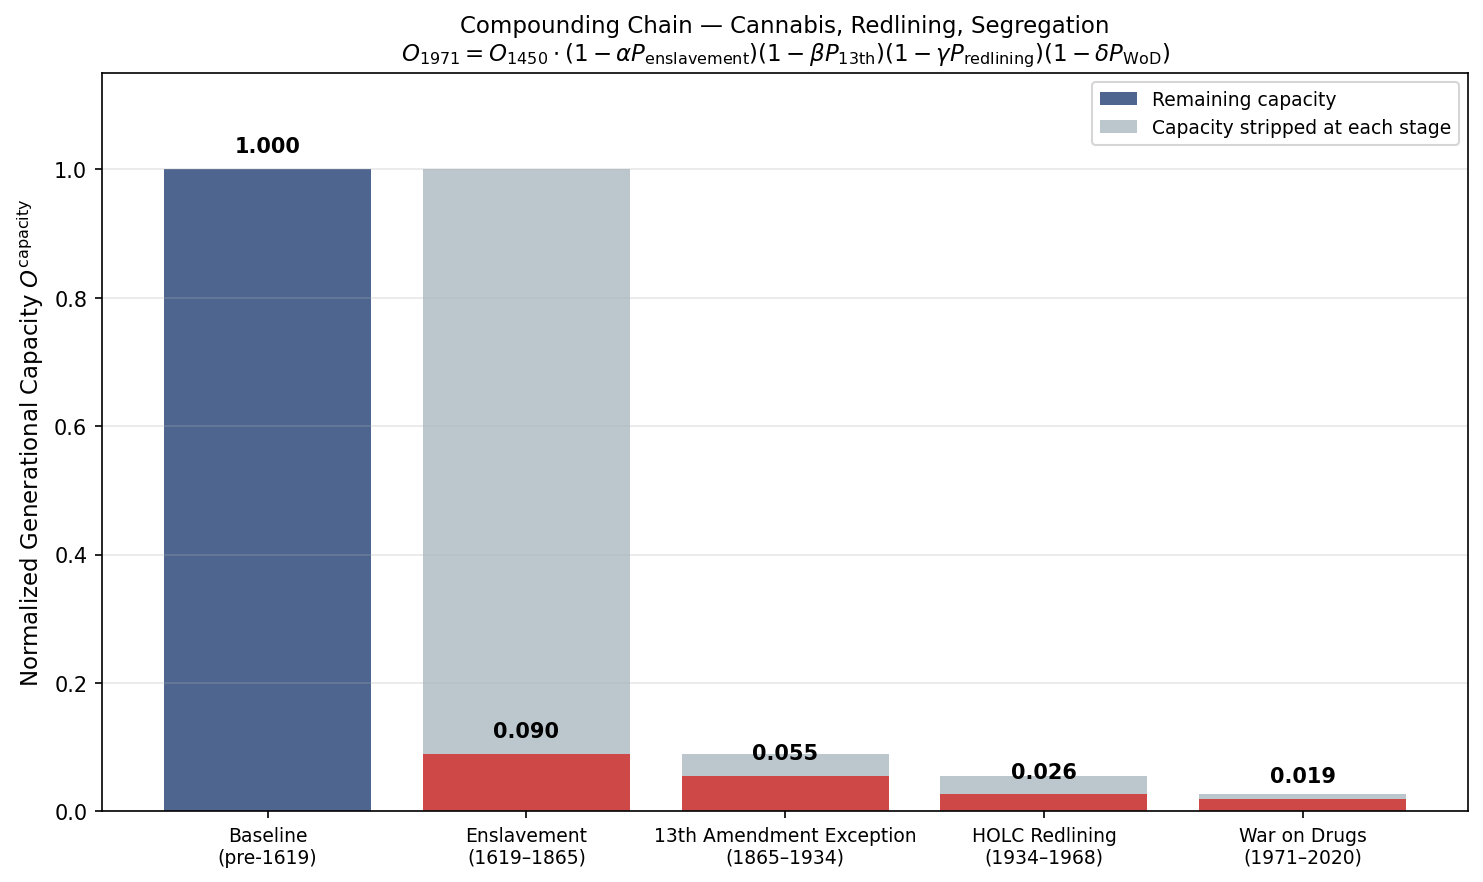
\includegraphics[width=0.92\textwidth]{figures/eq33_cannabis_redlining.png}
  \caption{Compounding capacity-reduction chain for eq.~\ref{eq:6.12-capacity-compounding-full}: each bar shows the residual $O^{\text{capacity}}$ after each policy shock, with the stripped capacity shown in grey. The four shocks compound from 1619 to 1971, producing a terminal $O_{1971} \approx 0.019$ --- less than 2\% of the normalized pre-contact baseline. Waterfall computed from ACLU (2020), Mapping Inequality, Blackmon (2008), and Darity \& Mullen (2020).}
  \label{fig:eq33_cannabis}
\end{figure}

\paragraph{Comparison to prediction.}
Equation~\ref{eq:6.12-capacity-compounding-full} predicts that the terminal wealth-capacity state is a direct mathematical consequence of the policy sequence. The data confirm this at every step: each factor is independently documented below 1.0; the cumulative product ($\approx 0.019$) is consistent with the observed Black-White wealth gap (median White household wealth $\approx 7.8\times$ Black, Federal Reserve SCF 2022), where the reparations-baseline approach of Darity \& Mullen anchors the expected ratio from the compounding model. The 3.73$\times$ cannabis arrest disparity (at equal usage rates) confirms that $\delta$ measures enforcement targeting, not behavioral difference.

\paragraph{Falsification criteria.}
This equation would be falsified if any one policy shock ($\alpha$, $\beta$, $\gamma$, $\delta$) is shown to have zero marginal effect on subsequent Black wealth accumulation in longitudinal data. Specifically: if controlling for the HOLC redlining shock eliminates the observed homeownership gap in difference-in-differences analysis, the $\gamma$ term collapses to zero and the compounding model fails. The existing literature (Rothstein 2017, Mapping Inequality geospatial data) finds the opposite: HOLC grade independently predicts present-day homeownership rates and neighborhood wealth levels after controlling for income, education, and other covariates.

\paragraph{Confidence tier.}
\textbf{Tier~1.} Each factor is independently documented in peer-reviewed or government-published literature; the ACLU cannabis arrest disparity is drawn from a national multi-year dataset controlling for usage rates; the HOLC homeownership gap is confirmed by geospatial overlay of federal archival records; the compounding product is directly computable from published figures without model assumptions.

\paragraph{Fractional-order memory: the continuous analogue.} The discrete multiplicative chain above is the sampled form of a fractional-order differential equation with Caputo derivative of order $\alpha \in (0,1)$, which governs agent dynamics in the formal containment model of Section~\ref{sec:formal-containment-model} \cite{li_mittag_leffler, kan_containment}. The Caputo derivative implements a \textbf{power-law memory kernel}: the present rate of change of $O^{\text{capacity}}$ is a weighted integral over its entire past trajectory, with weights decaying as $(t-s)^{-\alpha}$. The historical record is not overwritten by new policy; it is convolved with it. This is why the order of $P_1, \ldots, P_4$ above is non-commutative: each kernel is applied to the weighted history of every previous kernel. Mittag-Leffler stability (Theorem~\ref{thm:mittag-leffler}) then quantifies the shape of the resulting decay---slower than exponential, monotone, measured in generations rather than electoral cycles. Figure~\ref{fig:memory_gap} visualizes this distinction.

\begin{figure}[htbp]
\centering
\begin{tikzpicture}
\begin{axis}[
    width=0.95\textwidth,
    height=8cm,
    xmin=0, xmax=12,
    ymin=0, ymax=1.05,
    xlabel={Generations Since Initial Trauma},
    ylabel={Residual System Memory},
    xlabel style={font=\small},
    ylabel style={font=\small},
    title={\textbf{The Memory Gap: Fractional-Order vs.\ Integer-Order Decay}},
    title style={font=\bfseries\small},
    legend style={at={(0.97,0.97)}, anchor=north east, font=\scriptsize, fill=white, fill opacity=0.9, draw=gray},
    grid=major,
    grid style={gray!20},
    xtick={0,1,...,12},
    ytick={0,0.2,0.4,0.6,0.8,1.0},
]

\addplot[dashed, thick, black!50, samples=120, domain=0:12]
    {exp(-0.5*x)};
\addlegendentry{Integer-order $e^{-\lambda t}$ (what reformers assume)}

\addplot[very thick, red!85!black, samples=200, domain=0:12]
    {1/(1 + 0.65*x^0.5 + 0.25*x + 0.06*x^1.5 + 0.01*x^2)};
\addlegendentry{Fractional-order $E_{\alpha,1}(-\lambda t^{\alpha})$, $\alpha=0.5$ (actual memory)}

\draw[thick, blue!70, dashed] (axis cs:6,0) -- (axis cs:6,0.95);
\node[anchor=south, font=\scriptsize\bfseries, text=blue!70] at (axis cs:6,0.50) {$\approx$\,6 generations};
\node[anchor=south, font=\scriptsize, text=blue!70] at (axis cs:6,0.42) {since enslavement};

\draw[<->, thick, red!70] (axis cs:8,0.02) -- (axis cs:8,0.29);
\node[anchor=west, font=\scriptsize\bfseries, text=red!80!black] at (axis cs:8.1,0.155) {Memory Gap};

\node[anchor=west, font=\tiny, text=black!50, align=left] at (axis cs:7.5,0.06) {Integer model:\\``damage resolved''};

\node[anchor=east, font=\tiny, text=red!80!black, align=right] at (axis cs:11.5,0.22) {Fractional model:\\damage persists};

\end{axis}
\end{tikzpicture}
\caption{\textbf{The Memory Gap: Why Historical Damage Persists.} Under standard integer-order dynamics ($\alpha = 1$), a system's memory of initial conditions decays exponentially---the implicit assumption behind reform timelines that measure progress in electoral cycles. Under fractional-order dynamics ($\alpha = 0.5$), the Mittag-Leffler function decays as a power law: the memory of initial trauma persists across generations, with the residual far exceeding the integer-order prediction at every time horizon. At generation~6 (approximately the present distance from the end of chattel slavery), the integer model registers near-zero residual memory; the fractional model registers substantial ongoing structural deformation. The Middle Passage is not a recovered shock---it is a permanent deformation of the state trajectory.}
\label{fig:memory_gap}
\end{figure}

Crucially, while $O_{\text{racialized}}$ bears the primary compounding burden, the buffer class $I \setminus E$ is not immune. As the Predatory Min-Max Function exhausts extraction from $O_{\text{racialized}}$, the same compounding logic eventually turns inward: the tools developed to diminish $O_{\text{racialized}}$ are redeployed against $I \setminus E$, whose own capacity then begins to compound downward (see Section~6.12).

\begin{figure}[htbp]
\centering
\begin{tikzpicture}[scale=0.85, transform shape]
    % Timeline axis
    \draw[->, thick, gray] (-0.5,0) -- (14.5,0);
    \node[gray, font=\footnotesize] at (14.5,-0.4) {Time};

    % Capacity bars (staircase of decline)
    % 1450 baseline
    \fill[green!40] (0.2,0.1) rectangle (2.3,5.5);
    \draw[thick] (0.2,0.1) rectangle (2.3,5.5);
    \node[font=\footnotesize\bfseries, align=center] at (1.25,6.0) {1450\\{\scriptsize Baseline}};
    \node[font=\tiny, align=center] at (1.25,2.8) {$O_{1450}^{\text{cap}}$};

    % 1619 after enslavement
    \fill[yellow!40] (3.0,0.1) rectangle (5.1,4.0);
    \draw[thick] (3.0,0.1) rectangle (5.1,4.0);
    \node[font=\footnotesize\bfseries, align=center] at (4.05,6.0) {1619\\{\scriptsize Enslavement}};
    \node[font=\tiny, align=center] at (4.05,2.0) {$(1{-}\alpha P_{\text{ens}})$};
    \draw[->, very thick, red!60] (2.35,4.5) -- (2.95,4.5);

    % 1865 after 13th Amendment
    \fill[orange!40] (5.8,0.1) rectangle (7.9,2.8);
    \draw[thick] (5.8,0.1) rectangle (7.9,2.8);
    \node[font=\footnotesize\bfseries, align=center] at (6.85,6.0) {1865\\{\scriptsize 13th Amend.}};
    \node[font=\tiny, align=center] at (6.85,1.4) {$(1{-}\beta P_{\text{13th}})$};
    \draw[->, very thick, red!60] (5.15,3.3) -- (5.75,3.3);

    % 1934 after redlining
    \fill[red!30] (8.6,0.1) rectangle (10.7,1.8);
    \draw[thick] (8.6,0.1) rectangle (10.7,1.8);
    \node[font=\footnotesize\bfseries, align=center] at (9.65,6.0) {1934\\{\scriptsize Redlining}};
    \node[font=\tiny, align=center] at (9.65,0.95) {$(1{-}\gamma P_{\text{red}})$};
    \draw[->, very thick, red!60] (7.95,2.2) -- (8.55,2.2);

    % 1971 after War on Drugs
    \fill[red!50] (11.4,0.1) rectangle (13.5,1.0);
    \draw[thick] (11.4,0.1) rectangle (13.5,1.0);
    \node[font=\footnotesize\bfseries, align=center] at (12.45,6.0) {1971\\{\scriptsize War on Drugs}};
    \node[font=\tiny, align=center] at (12.45,0.55) {$(1{-}\delta P_{\text{WoD}})$};
    \draw[->, very thick, red!60] (10.75,1.3) -- (11.35,1.3);

    % Declining envelope line
    \draw[dashed, thick, red!70] (2.3,5.5) -- (5.1,4.0) -- (7.9,2.8) -- (10.7,1.8) -- (13.5,1.0);

    % Y-axis label
    \node[rotate=90, font=\footnotesize, gray] at (-0.9,2.8) {$O_t^{\text{capacity}}$ (accumulated capital, power, resources)};

    % Bottom annotation
    \node[font=\scriptsize, align=center, gray] at (7.0,-1.0) {Each policy compounds on an \textit{already diminished} baseline---the order is not interchangeable};
\end{tikzpicture}
\caption{\textbf{The Staircase of Decline: Historical Compounding of Out-Group Capacity.} Each policy reduces $O_t^{\text{capacity}}$ multiplicatively, not additively. The bars show how each successive policy---enslavement (1619), the 13th Amendment loophole (1865), redlining (1934), and the War on Drugs (1971)---compounds on an already diminished baseline, making the present condition of $O_{\text{racialized}}$ a mathematical inevitability of the policy sequence.}
\label{fig:historical_compounding}
\end{figure}

\begin{figure}[htbp]
\centering
\begin{tikzpicture}[every node/.style={font=\small}]
    % Capacity boxes
    \node[draw, thick, fill=green!30, minimum width=3cm, minimum height=2.8cm] (o0) at (0,0) {$O_0^{\text{capacity}}$};
    \node[draw, thick, fill=yellow!25, minimum width=3cm, minimum height=2.8cm, right=3.8cm of o0] (o1) {$O_1^{\text{capacity}}$};
    \node[draw, thick, fill=orange!30, minimum width=3cm, minimum height=2.8cm, right=3.8cm of o1] (o2) {$O_2^{\text{capacity}}$};

    % Capacity equations
    \node[font=\footnotesize] at ($(o1)+(0,-0.7)$) {$=\, O_0 \cdot (1-\alpha P_1)$};
    \node[font=\footnotesize] at ($(o2)+(0,-0.7)$) {$=\, O_1 \cdot (1-\beta P_2)$};

    % Policy arrows
    \draw[->, very thick, red] (o0.east) -- (o1.west);
    \draw[->, very thick, red] (o1.east) -- (o2.west);
    \node[red, font=\normalsize, align=center] at ($(o0)!0.5!(o1)+(0,1.0)$) {Policy $P_1$\\\footnotesize(enslavement)};
    \node[red, font=\normalsize, align=center] at ($(o1)!0.5!(o2)+(0,1.0)$) {Policy $P_2$\\\footnotesize(redlining)};

    % Time labels
    \node[font=\normalsize] at ($(o0)+(0,-1.9)$) {Time $t=0$};
    \node[font=\normalsize] at ($(o0)+(0,-2.35)$) {(initial)};

    \node[font=\normalsize] at ($(o1)+(0,-1.9)$) {Time $t=1$};
    \node[font=\normalsize, red] at ($(o1)+(0,-2.35)$) {(diminished)};

    \node[font=\normalsize] at ($(o2)+(0,-1.9)$) {Time $t=2$};
    \node[font=\normalsize, red] at ($(o2)+(0,-2.35)$) {(compounded)};

    % Visual representation of shrinking
    \draw[<->, thick, blue] ($(o0)+(-1.55,-3)$) -- ($(o0)+(1.55,-3)$);
    \node[blue, font=\normalsize] at ($(o0)+(0,-3.25)$) {Full capacity};

    \draw[<->, thick, blue] ($(o1)+(-1.55,-3)$) -- ($(o1)+(1.55,-3)$);
    \node[blue, font=\normalsize] at ($(o1)+(0,-3.25)$) {Reduced};

    \draw[<->, thick, blue] ($(o2)+(-1.55,-3)$) -- ($(o2)+(1.55,-3)$);
    \node[blue, font=\normalsize] at ($(o2)+(0,-3.25)$) {Severely reduced};

    % Annotation
    \node[align=center, font=\small] at ($(o1)+(0,-4.55)$) {$P_2$ applied to \textit{already diminished} group\\$\Rightarrow$ compounding harm, not additive};
\end{tikzpicture}
\caption{Temporal compounding model: Each policy reduces Out-group capacity, making subsequent policies more harmful. Policy $P_2$ (redlining) causes greater harm when applied to a group already diminished by $P_1$ (enslavement). As the system exhausts extraction from $O_{\text{racialized}}$, this same compounding mechanism is eventually turned against $I \setminus E$ (Section~6.12).}
\label{fig:compounding}
\end{figure}

\begin{figure}[htbp]
\centering
\begin{tikzpicture}[scale=0.92, transform shape]
    % --- Tier boxes (bottom to top = O to E) ---
    % Left edges stagger inward (pyramid shape); right edges align at 5.5 to contain text
    % O_racialized (bottom, widest)
    \fill[red!15] (-5.5,-0.4) rectangle (5.5,1.2);
    \draw[thick, red!70] (-5.5,-0.4) rectangle (5.5,1.2);
    \node[font=\bfseries, anchor=west] at (-5.3,0.4) {$O_{\text{racialized}}$};
    \node[font=\scriptsize, align=left, anchor=west] at (-1.2,0.4) {Racialized Out-group --- maximal policy contact,\\minimal lethal autonomy, extraction target};

    % I_buffer
    \fill[orange!15] (-4.8,1.6) rectangle (5.5,3.2);
    \draw[thick, orange!70] (-4.8,1.6) rectangle (5.5,3.2);
    \node[font=\bfseries, anchor=west] at (-4.6,2.4) {$I_{\text{buffer}}$};
    \node[font=\scriptsize, align=left, anchor=west] at (-1.2,2.4) {Buffer Class --- psychological wage, partial rights,\\absorbs $O$ anger, now entering cannibalization};

    % F_enforce
    \fill[blue!12] (-4.1,3.6) rectangle (5.5,5.4);
    \draw[thick, blue!60] (-4.1,3.6) rectangle (5.5,5.4);
    \node[font=\bfseries, anchor=west] at (-3.9,4.5) {$F_{\text{enforce}}$};
    \node[font=\scriptsize, align=left, anchor=west] at (-0.4,4.5) {Enforcement Class --- police, military,\\carceral system; deploys $P$ against $O$ and $I$;\\{\itshape no legal duty to protect} (\textit{Castle Rock},\\\textit{DeShaney})};

    % P_uppet
    \fill[green!10] (-3.4,5.8) rectangle (5.5,7.4);
    \draw[thick, green!50!black!50] (-3.4,5.8) rectangle (5.5,7.4);
    \node[font=\bfseries, anchor=west] at (-3.2,6.6) {$P_{\text{uppet}}$};
    \node[font=\scriptsize, align=left, anchor=west] at (-1.2,6.6) {Puppet Class --- elected officials,\\visible governance; expendable};

    % E (top, narrowest left edge but extends right to contain text)
    \fill[black!8] (-2.4,7.8) rectangle (5.5,9.4);
    \draw[thick, black!70] (-2.4,7.8) rectangle (5.5,9.4);
    \node[font=\bfseries, anchor=west] at (-2.2,8.6) {$E$};
    \node[font=\scriptsize, align=left, anchor=west] at (-1.2,8.6) {Elite --- extraction beneficiary,\\invisible, systemically immune};

    % --- Extraction arrows (upward, left side) ---
    \draw[->, very thick, red!70] (-5.8,1.2) -- (-5.8,3.2);
    \draw[->, very thick, red!70] (-5.8,3.2) -- (-5.8,5.4);
    \draw[->, very thick, red!70] (-5.8,5.4) -- (-5.8,7.4);
    \draw[->, very thick, red!70] (-5.8,7.4) -- (-5.8,9.2);
    \node[rotate=90, font=\footnotesize\bfseries, red!70] at (-6.4,5.0) {EXTRACTION ($\max$)};

    % --- Control arrows (downward, right side) ---
    \draw[->, very thick, blue!60] (5.8,9.2) -- (5.8,7.4);
    \draw[->, very thick, blue!60] (5.8,7.4) -- (5.8,5.4);
    \draw[->, very thick, blue!60] (5.8,5.4) -- (5.8,3.2);
    \draw[->, very thick, blue!60] (5.8,3.2) -- (5.8,1.2);
    \draw[->, very thick, blue!60] (5.8,1.2) -- (5.8,-0.2);
    \node[rotate=270, font=\footnotesize\bfseries, blue!60] at (6.4,5.0) {CONTROL ($\min$-management)};

    % --- Policy variable annotations (right side, between tiers) ---
    \node[font=\scriptsize, gray, align=center] at (7.8,0.0) {$P_{\text{criminal}}, P_{\text{spatial}}$\\$P_{\text{WarOnDrugs}}$};
    \draw[->, thin, gray] (6.1,0.4) -- (6.9,0.2);

    \node[font=\scriptsize, gray, align=center] at (7.8,2.0) {$P_{\text{grandfather}}$\\$P_{\text{gaslight}}$};
    \draw[->, thin, gray] (6.1,2.4) -- (6.9,2.2);

    % --- Lethal autonomy gradient (far left) ---
    \draw[<-, thick, black!50] (-7.2,-0.4) -- (-7.2,9.4);
    \node[rotate=90, font=\scriptsize, black!50] at (-7.7,4.5) {Lethal Autonomy ($L$)};
    \node[font=\tiny, black!50] at (-7.2,-0.7) {$L_O \to 0$};
    \node[font=\tiny, black!50] at (-7.2,9.7) {$L_E = \max$};

    % --- Cannibalization zone annotation ---
    \draw[thick, dashed, red!50] (-5.5,1.4) -- (5.5,1.4);
    \node[font=\tiny\itshape, red!50, anchor=east] at (5.4,1.5) {cannibalization threshold (expanding upward)};

\end{tikzpicture}
\caption{\textbf{The 5-Tier Extraction Hierarchy.} The Predatory Min-Max Function operates through five nested tiers. Extraction ($\max$) flows upward from $O_{\text{racialized}}$ to $E$; control ($\min$-management) flows downward through policy variables ($P$) deployed by $F_{\text{enforce}}$ at the direction of $P_{\text{uppet}}$, which is itself expendable to $E$. Lethal autonomy increases from bottom to top. The dashed line marks the cannibalization threshold: as extraction exhausts $O_{\text{racialized}}$, the system expands its extraction zone upward into $I_{\text{buffer}}$, consuming the Buffer Class it originally created to protect itself.}
\label{fig:venn_model}
\end{figure}

This five-tier structure (Figure~\ref{fig:venn_model}) maps the full architecture of the Predatory Min-Max Function: extraction flows upward from the racialized Out-group to the Elite, while control flows downward through policy variables deployed by the Enforcement Class. The cannibalization threshold marks the system's current phase---expanding extraction beyond $O_{\text{racialized}}$ into the Buffer Class itself.

\section{The Unbroken Financial Lineage: From Slave Mortgages to Carceral Bonds}

The 13th Amendment's variable swap from racial identity to criminal status was not merely a legal maneuver---it preserved an entire financial architecture. To understand the continuity, we must trace the capital pipeline from its antebellum origin.

That prison labor remains a federally regulated commodity---not a historical footnote---is visible in \usclink{apx:usc:18:1761}{18 U.S.C.~\S~1761}, which governs the interstate commerce of goods manufactured by convicts:
\uscinline{usc_18_1761}

Northern banks, insurance companies, and merchants profited enormously from financing and insuring the slave trade and slave-based production. Bonnie Martin's analysis of nearly 9,000 antebellum mortgages found that \textbf{47 percent involved enslaved human beings as collateral} \cite{martin}---revealing that the mortgage of human property was not peripheral but the \textit{invisible engine} of Southern capital formation.

The most striking case is that of \textbf{Citizens Bank and Canal Bank of Louisiana}, which collectively accepted approximately 13,000 enslaved people as mortgage collateral and directly owned more than 1,200 human beings \cite{baptist, murphy}. In 1836, the State of Louisiana issued \textbf{state-backed bonds} collateralized by these slave mortgages and marketed them to investors across Europe---through firms such as Baring Brothers in London, Amsterdam, and Paris. These instruments were, in function, \textbf{mortgage-backed securities} whose underlying ``assets'' were human beings. Both banks are now predecessor institutions of JPMorgan Chase.

This financial architecture did not disappear with the 13th Amendment---it \textit{evolved}. By 1860, enslaved people represented the largest single asset class in the United States, worth more than all manufacturing and railroads combined \cite{baptist, beckert}. The 13th Amendment did not destroy this capital---it merely rerouted it through the carceral system.

To see the continuity, we must trace the complete cash-flow pipeline in both eras and demonstrate that the \textit{string}---the unbroken thread connecting human body to financial instrument to investor---has never been cut. It has only been re-encoded.

\subsection{The Old String: Slave-Backed Securities (1830s--1865)}

The antebellum pipeline operated as follows:

\begin{enumerate}
    \item \textbf{The Asset}: An enslaved human being, legally classified as moveable property.
    \item \textbf{The Collateralization}: The enslaved person is mortgaged---pledged as collateral for a loan. Martin documents that 47\% of antebellum mortgages involved enslaved people as collateral \cite{martin}.
    \item \textbf{The Securitization}: Banks bundle these slave mortgages into state-backed bonds. Louisiana issues bonds collateralized by the slave portfolios of Citizens Bank and Canal Bank, marketed through Baring Brothers to investors in London, Amsterdam, and Paris \cite{murphy}.
    \item \textbf{The State Guarantee}: The state backs the instruments---its full faith and credit standing behind the return on investment.
    \item \textbf{The Revenue Stream}: The investor receives a guaranteed return. The return is generated by the labor extracted from the enslaved person's body.
    \item \textbf{The Enforcement}: Slave patrols ($F_{\text{enforce}}^{\text{v1.0}}$) function as \textit{asset recovery agents}---retrieving runaways (lost assets), suppressing revolts (protecting the portfolio), and maintaining the labor discipline that generates the revenue stream backing the bonds.
\end{enumerate}

The cash flow is: \textbf{Body $\rightarrow$ Labor $\rightarrow$ Revenue $\rightarrow$ Bond $\rightarrow$ Investor}. The state guarantees the instrument. The Enforcement Class protects the asset. The Elite in Europe sips tea while the return-on-investment is generated by the lash.

\subsection{The New String: Carceral Bonds (1983--Present)}

The modern pipeline replicates this structure with updated variable names:

\begin{enumerate}
    \item \textbf{The Asset}: An incarcerated human being, legally reclassified from ``slave'' to ``inmate'' via the 13th Amendment's exception clause.
    \item \textbf{The Collateralization}: Private prison companies (CoreCivic, GEO Group) issue bonds and revenue instruments whose value depends on maintaining incarcerated populations \cite{alexander}. Each occupied bed generates a per-diem payment from the state---typically \$50--\$150 per day per inmate.
    \item \textbf{The Securitization}: These revenue streams are packaged into financial instruments---corporate bonds, REITs (Real Estate Investment Trusts), and equity offerings---traded on public markets. CoreCivic and GEO Group are publicly traded on the New York Stock Exchange.
    \item \textbf{The State Guarantee}: Private prison contracts contain \textbf{occupancy guarantee clauses}---typically requiring the state to maintain \textbf{80--90\% bed occupancy} or pay for the empty beds regardless \cite{itpi}. The state's full faith and credit once again backs the instrument. If the beds are not filled with bodies, the taxpayer pays the difference.
    \item \textbf{The Revenue Stream}: The investor receives a guaranteed return. CoreCivic reported \$1.99 billion in revenue in 2022; GEO Group reported \$2.42 billion. These are not abstract financial numbers---they are the monetized output of human incarceration.
    \item \textbf{The Enforcement}: Police ($F_{\text{enforce}}$) function as \textit{asset acquisition agents}---filling the beds that back the bonds, meeting the quotas that satisfy the occupancy clauses, generating the bodies that produce the revenue stream that pays the investors.
\end{enumerate}

The cash flow is identical: \textbf{Body $\rightarrow$ Incarceration $\rightarrow$ Revenue $\rightarrow$ Bond $\rightarrow$ Investor}. The state guarantees the instrument. The Enforcement Class acquires the asset. The variable names changed; the string did not.

\subsection{The Demand Signal: How Financial Instruments Manufacture Crime}

The occupancy guarantee clause is the load-bearing variable that converts the carceral system from a public safety institution into a \textit{demand-driven asset pipeline}. Trace the causal chain:

\begin{enumerate}
    \item $E$ (the Elite) invests in private prison bonds, expecting a 7--10\% annual return.
    \item The return depends on beds being occupied. The private prison contract guarantees 90\% occupancy.
    \item The state must deliver bodies to fill those beds---or pay for the empty ones.
    \item The state directs $F_{\text{enforce}}$ (police departments) to meet arrest quotas calibrated to the occupancy requirements.
    \item $F_{\text{enforce}}$ requires a legal mechanism to generate arrests at scale. The Puppet Class ($P_{\text{uppet}}$) has already provided one: the legislative web of Universal Latent Criminality documented in Chapter~\ref{ch:full_algo}. The average American commits an estimated three felonies per day without knowing it \cite{silverglate}. The law is written so broadly that \textit{everyone} is a potential arrest---the system merely selects \textit{which} bodies to process.
    \item $F_{\text{enforce}}$ exercises selective enforcement---choosing from the full glossary of available charges to fill the beds. The selection is not random. It follows the path of least resistance: $O_{\text{racialized}}$ first (the population with the least political and legal capital to resist), then the lower strata of $I_{\text{buffer}}$ as the extraction zone expands.
\end{enumerate}

This is why the police have \textit{no legal duty to protect you} (Castle Rock, DeShaney). They were never designed to protect. They were designed---from the slave patrols of the 18th century to the quota-driven departments of the 21st---to \textit{acquire and maintain assets} for the financial instruments that sit at the top of the extraction pipeline. The ``no duty to protect'' doctrine is not a bug in the system. It is the system telling you, through its own case law, exactly what $F_{\text{enforce}}$ was built to do.

The demand signal flows \textit{downward} through the hierarchy: $E$ demands returns $\rightarrow$ private prisons demand bodies $\rightarrow$ state guarantees occupancy $\rightarrow$ police departments enforce quotas $\rightarrow$ prosecutors stack charges $\rightarrow$ bodies enter the pipeline. The supply of ``crime'' is manufactured to meet the demand of capital. This is not a conspiracy---it is a market. The incarcerated human being is the commodity. The bond is the instrument. The state is the guarantor. The police are the supply chain.

And here is the structural revelation: \textit{the string has never been cut}. From the 1836 Louisiana slave bond purchased by a London banker to the 2026 CoreCivic corporate bond purchased by a hedge fund manager, the pipeline is continuous. A human body enters the system. Its captivity generates revenue. That revenue is securitized into a financial instrument. The instrument is sold to an investor. The investor receives a return. The Enforcement Class ensures the supply. The state guarantees the product.

The only thing that changed was the legal classification of the body at the point of entry. The 13th Amendment's ``except as a punishment for crime'' clause did not end slavery. It \textit{privatized the front end and securitized the back end}. The rest of the string---from body to bond to investor---remained structurally, financially, and morally identical.

\section{Imperial Enforcement: The 1915 Occupation and the Resurrection of the Corv\'{e}e}
\label{sec:haiti_occupation}

To understand the full scope of the Buffer Class's enforcement role, one must examine how the Elite deploys nominal In-group members across sovereign borders. The United States occupation of Haiti (1915–1934) perfectly models the corporate weaponization of the state. The pre-1915 arc---Haiti's material export of liberation to Gran Colombia, Mexico, the Dominican Republic, and Greece; the vexillological encoding of revolutionary solidarity; and the Firmin Protocol's 1891 diplomatic repulsion of U.S. naval coercion---is documented in Chapter~\ref{ch:haitian_export}. The 1915 occupation represents the Elite's recursive answer to that full counter-strategy: when the financial and legal mechanisms proved insufficient to neutralize $O_{\text{emancipated}}$'s institutional capacity, the enforcement mechanism was deployed in its most direct form.

The occupation was not driven by democratic state-building, but by the financial imperatives of the American Elite, specifically Wall Street institutions like National City Bank (now Citibank). The US military—functioning as the ultimate, transnational manifestation of the slave patrol—was deployed to seize Haiti's gold reserves, commandeer its customs houses, and forcibly rewrite its constitution to allow foreign land ownership.

Once in control, the occupying forces immediately reinstated the \textit{corv\'{e}e}, a system of forced, unpaid labor utilized to build infrastructure for the benefit of foreign corporate interests. This demonstrates the algorithmic consistency of the Elite's operating system. Just as the 13th Amendment loophole was utilized domestically to re-enslave Black Americans through the carceral state, the US military utilized imperial law to institute forced labor upon the Haitian population. The extraction of Black labor for the benefit of white capital ($E$) was forcefully resumed, masked entirely behind the ideological justification (Component 3) of ``modernization'' and ``civilization.''

\section{The Geographic Displacement of Slave Capitalism}

The Haitian occupation reveals a broader structural truth: \textbf{slave capitalism did not end with industrial capitalism}---rather, industrial capitalism \textit{is} slave capitalism, merely evolved and geographically dispersed. What changed after formal abolition was not the elimination of slavery but its \textbf{geographic displacement} and legal obfuscation. After centuries of extracting African bodies as slaves, capitalism now extracts African labor \textit{in situ}---keeping the exploitation in Africa while extracting the value. Former colonial powers use structural adjustment, debt, and military coercion to maintain exploitative relationships that replicate the extraction kernel across sovereign borders.

\subsection{Case Study: France's Dependence on African Exploitation}

The contemporary crisis in French-African relations exposes this dependency with mathematical precision. France's economy has long relied on:

\begin{itemize}
    \item \textbf{CFA Franc system}: 14 African nations forced to use currency controlled by the French Treasury, required to deposit 50--85\% of their reserves in France \cite{pigeaud}, giving France de facto control over their monetary policy
    \item \textbf{Resource extraction contracts}: Uranium from Niger powers French nuclear plants (70\% of French electricity); France pays far below market rates under contracts established during the colonial period
    \item \textbf{Military enforcement}: France maintains military bases across former colonies to protect these arrangements, intervening militarily whenever governments attempt to renegotiate
\end{itemize}

As of 2023--2024, multiple African nations (Niger, Mali, Burkina Faso, Gabon) have expelled French military, rejected the CFA Franc, and nationalized resources. France's economy is experiencing serious strain---energy crisis, loss of captive markets, capital flight, and inflation from paying market rates for resources previously extracted at colonial prices. This demonstrates that \textbf{Western industrial capitalism would collapse without access to exploited African labor and resources}. The system is not post-slavery; it is slavery with better PR.

The extraction function remains continuous: the ``asset class'' changed its legal designation from ``slave'' to ``debtor nation''; the Predatory Min-Max Function remained intact. The Elite ($E$) traces an unbroken financial lineage from antebellum planters who securitized enslaved bodies, to colonial administrators who extracted resources through military occupation, to modern multinational corporations that extract through debt instruments and trade agreements. The variable $E$ has merely globalized; the kernel has never been modified.

\part{Scaling and Runtime (1865--Present)}
\label{part:runtime}

\chapter{The Containment: Pullman, Redlining, and the Wages of Whiteness (1894--1965)}
\label{ch:containment}

\begin{tcolorbox}[colback=black!5, colframe=black!70, fonttitle=\bfseries\ttfamily, title=RUNTIME LOG: 1894--1965 (POST-EMANCIPATION CONTAINMENT)]
\ttfamily\small
\textbf{System Stress} ($\min$: class resistance): HIGH --- 13th Amendment reclassified $O_{\text{racialized}}$ as citizens with voting rights. Parallel Out-group economy emerging. Civil Rights Movement breaching the legal interface.\\
\textbf{Capital} ($\max$: extraction output): RESTRUCTURING --- Direct slavery terminated. System transitioning to indirect extraction via convict leasing, sharecropping, and spatial containment.\\
\textbf{Interference State} ($\Phi_{\text{load}}$, proximity to $\tau$): $\Phi_{\text{load}} \in [0.55, 0.72]$; $\rho_{\tau} \in [0.50, 0.68]$.\\
\textbf{Variables Loaded}: $E$, $O_{\text{racialized}}$, $I$, $I_{\text{buffer}}$, $F_{\text{enforce}}$.\\
\textbf{Variables Deployed This Cycle}: $\psi$ (psychological wage, weaponized), $P_{\text{spatial}}$ (Redlining), Capture Variable.\\
\textbf{Executing Function}: Terminate the Out-group's parallel economy (Tulsa 1921, East St.\ Louis 1917). Build the containment field $P_{\text{spatial}}$ (National Housing Act 1934). Absorb the Civil Rights Movement's legal victories into two-party loyalty without dismantling the extraction kernel.\\
\textbf{Result}: \textbf{[POLICY]} HOLC Redlining (1934) concentrates $O_{\text{racialized}}$ for targeted extraction. \textbf{[POLICY]} Civil Rights Act (1964) and Voting Rights Act (1965) dismantle the legal interface but leave the kernel untouched. Capture Variable absorbs $O_{\text{racialized}}$ into the two-party system. $\min$ restored through spatial and political containment. The Puppet Class upgrade that coordinates these moves is deployed in Chapter~\ref{ch:tweedism}.
\end{tcolorbox}

\medskip

The 13th Amendment terminated direct slavery but did not terminate extraction. The Elite ($E$) needed a containment architecture that could hold a newly enfranchised Out-group ($O_{\text{racialized}}$) inside the extraction zone without the explicit legal interface of chattel ownership. This chapter traces three moves that built that architecture: (i) the 1894 Pullman Strike, in which the Buffer Class's investment in the psychological wage ($\psi$) destroyed the one labor coalition that could have toppled industrial capital; (ii) the 1917--1934 kinetic and legal operations---Tulsa, East St.\ Louis, the National Housing Act---that terminated the Out-group's parallel economy and compressed it into redlined containment fields; and (iii) the mid-twentieth-century Capture Variable, through which the Civil Rights Movement's legal victories were absorbed into two-party political loyalty without disturbing the extraction kernel. Chapter~\ref{ch:tweedism} then takes up the democratic front-end that coordinates these moves: the industrialized Puppet Class ($P_{\text{uppet}}$) and the Tweedism Filter.

Containment gives the mind virus a map. Redlining, sundown towns, school boundaries, restrictive covenants, and urban-renewal clearance did not merely allocate space; they trained perception by making race, risk, poverty, policing, and property value appear to occupy the same coordinates. The host wetware then learned the geography as if it were evidence: this neighborhood is dangerous, that school is failing, this applicant is risky. Spatial policy became cognitive firmware.

The deeper context for this chapter is provided by Du Bois's analytical architecture in \textit{Black Reconstruction} \cite{dubois}. Du Bois argued that Reconstruction (1865--1877) was not merely a political experiment that failed---it was a successful multiracial democracy that was \textit{overthrown} by a coordinated counter-revolution of property. The critical mechanism was not Southern racism per se but Northern capital's recognition that the Reconstruction governments' labor and land reforms threatened industrial extraction at the national scale. The railroad magnates, industrial financiers, and Northern Republican machine that had fought to end slavery quickly made common cause with Southern Redeemer Democrats the moment Black political power threatened to raise labor standards and redistribute land. Du Bois named this the ``counter-revolution of property'': the restoration of the extraction kernel through elite-class alliance across the racial partition the Elite had previously used to divide the laboring class. This chapter's three case studies---Pullman, redlining, and the Capture Variable---are the post-1877 continuation of that counter-revolution: the same Elite interest in containing cross-racial democracy, now operating through capital rather than paramilitary violence.

We begin with the Gilded Age's most elegant proof that the Buffer Class's investment in $\psi$ is \textit{self-defeating}---a case where the white working class's refusal to organize across the racial partition handed the Elite the precise weapon needed to destroy them.

\section{The Pullman Strike: How the Psychological Wage Broke the Working Class (1894)}

In 1894, the Pullman Palace Car Company---manufacturer of the luxury sleeping cars that defined American rail travel---slashed wages by 25 percent while refusing to reduce rents in the company town of Pullman, Illinois, where workers were compelled to live. Workers who earned \$9 per week received paychecks of \$0.07 after rent was deducted. The material conditions were objectively intolerable \cite{lindsey_pullman, salvatore_debs}.

Eugene V. Debs, leader of the newly formed American Railway Union (ARU), organized a national boycott: ARU members across the country refused to handle any train with a Pullman car attached. Within days, rail traffic across 27 states ground to a halt. Railroad profits collapsed. The strike was \textit{working}.

Here is where the popular narrative---recently recirculated through social media---claims that this was ``America's first successful integrated strike,'' with Black Pullman porters and white railroad workers standing together in unified action. \textbf{This is historically false, and the actual record is far more damning.}

The ARU was a \textbf{whites-only union}. At its 1893 founding convention, the membership voted to restrict enrollment to white railroad employees, overriding Debs's personal objections \cite{salvatore_debs, arnesen_waterfront}. Black workers---including the Pullman porters who suffered under some of the most exploitative conditions in the industry---were categorically excluded from the organization that claimed to represent all railroad labor.\footnote{Du Bois had already diagnosed this structural pathology in \textit{Black Reconstruction} \cite{dubois}, tracing the same dynamic through the collapse of the Knights of Labor in the 1880s. The Knights briefly admitted Black workers on an integrated basis; the AFL's founding in 1886 reversed that policy, institutionalizing craft-union exclusion at precisely the moment when industrial unionism could have built durable cross-racial power. The ARU's 1893 exclusion was not a new error---it was the same capitulation to $\psi$ that Du Bois had already identified as the primary mechanism by which white labor forfeited its material leverage to Elite capital.}

Within the framework, this is the psychological wage ($\psi$) operating at the institutional level. The white working class was offered a choice: build a union that included $O_{\text{racialized}}$ and maximize collective bargaining power, or build a union that excluded $O_{\text{racialized}}$ and preserve racial status hierarchy. They chose $\psi$. They chose whiteness over power.

\subsection{Capital Weaponizes the Partition}

The Elite ($E$)---organized through the \textbf{General Managers' Association (GMA)}, a consortium of 24 railroad companies---immediately exploited the racial partition the ARU had built into its own architecture. The GMA actively recruited Black workers as strikebreakers, offering the very jobs the ARU had refused to share \cite{arnesen_waterfront, lindsey_pullman}.

The mathematical logic was devastating:
\begin{enumerate}
    \item The ARU excluded Black workers from the union ($O_{\text{racialized}} \notin \text{ARU}$).
    \item Black workers therefore had zero institutional loyalty to the strike and rational economic incentive to accept replacement positions.
    \item The GMA deployed excluded Black workers to cross picket lines, simultaneously breaking the strike \textit{and} inflaming the racial resentment that had produced the exclusion in the first place.
\end{enumerate}

The Elite did not need to \textit{create} the racial division. The Buffer Class had pre-installed it. Capital merely \textit{weaponized} it. This is the framework's prediction operating in real time: the psychological wage ($\psi$) accepted by $I_{\text{buffer}}$ in exchange for policing the racial boundary is not a \textit{benefit}---it is a \textit{vulnerability} that $E$ exploits whenever class solidarity threatens extraction.

\subsection{The Manufactured Pretext: Mail Cars as Legal Fiction}

Even with strikebreakers deployed, the boycott was paralyzing the national rail system. The Elite required federal force. But there was a constitutional obstacle: Illinois Governor John Peter Altgeld---a progressive who understood the strike as a legitimate labor action---explicitly refused to request federal intervention, insisting that the state was fully capable of maintaining order \cite{lindsey_pullman}.

President Grover Cleveland had no constitutional invitation to act. The Puppet Class ($P_{\text{uppet}}$) needed a pretext.

The solution was architecturally elegant. The GMA \textit{deliberately attached Pullman passenger cars to trains carrying U.S.\ mail}. This was not accidental logistics---it was a calculated maneuver to ensure that any boycott of Pullman cars would simultaneously obstruct federal mail delivery. The railroad managers manufactured the very federal crisis they then asked the government to resolve \cite{lindsey_pullman, papke_pullman}.

Attorney General Richard Olney---himself a \textbf{former board member of multiple railroad companies} and a man who continued to receive a retainer from the Burlington Railroad while serving as the nation's chief law enforcement officer---secured a blanket federal injunction under the Sherman Antitrust Act, prohibiting Debs and the ARU from ``compelling or encouraging'' any interference with rail operations \cite{papke_pullman, salvatore_debs}.

The irony is structurally perfect: the Sherman Antitrust Act, ostensibly designed to prevent \textit{corporate} monopolies from crushing competition, was repurposed by a corporate attorney serving as Attorney General to crush a \textit{labor} union. The statute designed to restrain $E$ was deployed by $P_{\text{uppet}}$ to protect $E$. The interface was rewritten in real time.

\subsection{12,000 Troops: The Enforcement Class Protects Capital}

On July 3, 1894, President Cleveland deployed approximately 12,000 federal troops to Chicago under the command of Brigadier General Nelson Miles---over Governor Altgeld's furious written protest that the action was ``a violation of a basic principle of our institutions'' \cite{lindsey_pullman}.

The troops' stated mission was protecting mail delivery. Their actual operations told a different story: they guarded railroad property, escorted strikebreakers to their positions, and cleared workers from rail yards. The Enforcement Class ($F_{\text{enforce}}$) was executing capital protection under the legal fiction of postal security.

The strike collapsed. Debs was arrested, convicted of contempt for violating the injunction, and imprisoned. The Supreme Court, in \textit{In re Debs} (1895), unanimously upheld the federal government's authority to intervene, ruling that the government's power over interstate commerce and mail delivery justified the injunction regardless of whether state authorities had requested assistance \cite{inredebs}.

The judicial branch of $P_{\text{uppet}}$ retroactively blessed the entire operation. The precedent was set: when labor organization threatened capital extraction, the federal government could bypass state authority, deploy military force, and imprison labor leaders---all under manufactured legal pretexts validated after the fact by compliant courts.

\subsection{The Theorem the Buffer Class Refused to Learn}

The Pullman Strike proves a corollary of the Predatory Min-Max Function:

\begin{keyinsight}[The Pullman Corollary]
When $I_{\text{buffer}}$ excludes $O_{\text{racialized}}$ from collective action to preserve the psychological wage ($\psi$), the Elite ($E$) will weaponize the excluded population against $I_{\text{buffer}}$, ensuring both groups lose. The partition that $I_{\text{buffer}}$ builds to maintain status superiority over $O_{\text{racialized}}$ becomes the structural vulnerability through which $E$ destroys $I_{\text{buffer}}$'s material power.
\begin{equation}\label{eq:7.1-pullman-corollary}
\psi \uparrow \implies \text{Solidarity}(I_{\text{buffer}}, O_{\text{racialized}}) \downarrow \implies \text{Vulnerability}(I_{\text{buffer}}) \uparrow \implies \mathcal{E}(t) \uparrow
\end{equation}
\end{keyinsight}

The\footnote{This equation is classified as Tier~3 (ordinal/structural); the Pullman Corollary is a directional claim---that the psychological wage ($\psi$) suppresses cross-racial solidarity, increasing Buffer Class vulnerability to Elite extraction---validated by the Pullman Strike (1894) case, where AFL exclusion of Black workers enabled strikebreaker recruitment that defeated the strike. See Roediger (1991) \cite{roediger} and the Empirical Methodology chapter (p.~\pageref{ch:empirical_methodology}).} white railroad workers of 1894 chose the psychological wage and lost their material wages. The Elite extracted maximum value from both populations: Black workers received temporary strikebreaking employment with no union protections and no long-term security, while white workers lost the strike, lost their union, and lost their leader to a federal prison. Only $E$ won.

It would take another thirty-one years before Black Pullman porters---the workers the ARU had refused to organize alongside---built their own autonomous institution. In 1925, A.\ Philip Randolph founded the \textbf{Brotherhood of Sleeping Car Porters (BSCP)}, which in 1937 became the first African American labor union to negotiate a collective bargaining agreement with a major American corporation \cite{bates_pullman}. The BSCP did not wait for the Buffer Class to invite them into solidarity. They built power independently---and that independent power base became a critical institutional infrastructure of the Civil Rights Movement.

The lesson the framework extracts: cross-racial solidarity is not a moral aspiration---it is a \textbf{strategic necessity}. Without it, the extraction kernel runs unopposed.

This is the framework's answer to any analysis that treats the Great Migration's labor competition or wartime industrial demand as alternative explanations for the violence documented in this chapter. Material economic pressure is not in competition with $\psi$---it is $\psi$'s activation context. The wartime economy created a genuine zero-sum competition for factory jobs, housing, and public space between $I_{\text{buffer}}$ and $O_{\text{racialized}}$. That competition could have been resolved in two directions: cross-racial class solidarity against the capital that depressed wages for both groups, or racial partition that redirected the pressure downward onto $O$. The Great Migration did not determine which resolution occurred. The psychological wage did. The material conditions set the pressure; $\psi$ determined the direction of discharge. Detroit in 1943 is not a story about industrial demand producing racial violence. It is a story about industrial demand producing labor competition, and $\psi$ routing that competition through the racial partition rather than the class partition---producing a result in which $E$ retained its labor supply at depressed wages, $I_{\text{buffer}}$ sacrificed war production to police the racial boundary, and $O$ bore the kinetic cost of a structural crisis the Elite's own containment architecture had manufactured. Material factors explain the pressure. Only $\psi$ explains why the pressure discharged downward.

\section{The Optimization: Redlining as the Containment Field (1934)}

Before we can understand redlining, we must understand what it was designed to \textit{destroy}---because the Out-group's response to exclusion from the white financial system was not passive suffering. It was the construction of an autonomous economic architecture so successful that the Elite had to deploy federal policy to dismantle it.

\subsection{The Out-group Builds a Parallel Economy (1900--1921)}

A critical misconception must be corrected: racial segregation and redlining are \textit{not the same thing}. Segregation---the spatial and social separation of $O_{\text{racialized}}$ from $I_{\text{buffer}}$---existed for decades before the Home Owners' Loan Corporation drew a single red line. But segregation alone was not sufficient to maintain extraction, because the Out-group did something the Elite's algorithm had not anticipated: they built an independent economic system \textit{within} the segregated space.

In 1900, Booker T.\ Washington founded the \textbf{National Negro Business League (NNBL)} in Boston, organizing Black entrepreneurs, professionals, and financiers into a coordinated economic network \cite{washington_nnbl}. By 1915, the NNBL had grown to over 600 chapters across 34 states, spawning affiliated institutions that constituted a parallel financial infrastructure: the National Negro Bankers Association, the National Negro Insurance Association, the National Negro Press Association, the National Association of Negro Real Estate Dealers, and the National Negro Finance Corporation \cite{washington_nnbl, work_yearbook}.

The scale of this infrastructure is documented in the \textit{Negro Year Book} (1914--15), compiled by Monroe N.\ Work at the Tuskegee Institute: by 1913, Black Americans had established approximately \textbf{40,000 businesses} nationwide, alongside over 500,000 Black-owned properties \cite{work_yearbook}. These enterprises were not charity---they were \textbf{economic architecture}: Black banks in Alabama lending to Black farmers; Black manufacturers in Chicago supplying Black retailers in Atlanta; Black insurance companies pooling community risk when white insurers refused coverage. Fraternal orders and mutual aid societies---organizations dating to the antebellum period---provided burial insurance, widow's pensions, small loans, and community welfare services that the white state categorically denied to $O_{\text{racialized}}$ \cite{walker_business}.

The result was the emergence of thriving, economically autonomous Black districts: the Greenwood District in Tulsa (``Black Wall Street''), with over 100 Black-owned businesses by 1921; Parrish Street in Durham, anchored by the North Carolina Mutual Life Insurance Company (founded 1898) and the Mechanics and Farmers Bank; the Shaw corridor in Washington, D.C., hosting over 200 Black-owned businesses by 1910 \cite{walker_business, messer_tulsa}.

Within the framework, this autonomous infrastructure represented a \textbf{system-level threat}. The extraction kernel depends on the Out-group's economic dependency on institutions controlled by $E$. When $O_{\text{racialized}}$ built banks that did not require white capital, insurance companies that did not require white actuarial approval, and commercial networks that circulated wealth internally, the Elite faced a structural crisis: the Out-group was approaching \textit{economic escape velocity}---the point at which the extraction kernel could no longer reach them.

\subsection{Phase One---Kinetic Destruction: The Massacre Pattern (1866--1923)}

The Elite's first response was blunt and kinetic. When the Out-group accumulated visible wealth in identifiable geographic concentrations, the system deployed the Buffer Class ($I_{\text{buffer}}$) and the Enforcement Class ($F_{\text{enforce}}$) in coordinated acts of economic annihilation. This pattern did not begin in 1917; it is traceable in an unbroken line from the first moment Black autonomy became legible to the extraction kernel, beginning the week Reconstruction began. To understand the full weight of what was done, the events must be named---individually, in sequence---because the aggregate is the argument.

\subsubsection{The F.E.A.R. Score: Measuring the Demoralizing Signal}
\label{sec:fear_score}

Each massacre transmitted a \textbf{structured signal} to the entire Out-group. It was not merely a local atrocity; it was a \textbf{nationwide broadcast}. The framework captures this with a four-axis analytical tool:

\begin{tcolorbox}[
  colback=gray!5!white,
  colframe=gray!60!black,
  title={\textbf{F.E.A.R. Score: Axes of Systemic Terror}},
  fonttitle=\bfseries,
  breakable
]
\textbf{F --- Frequency and Geographic Spread}: How many discrete events, across how many cities and states, in what time span? High frequency proves the algorithm is not local but systemic---a distributed execution of a single kernel objective.\\[4pt]
\textbf{E --- Economic Annihilation}: What was the dollar value of autonomous Black wealth destroyed? How many businesses, homes, banks, schools, hospitals, and fraternal assets were liquidated? This axis measures the \textit{anti-accumulation incentive} installed in every surviving Black community nationwide.\\[4pt]
\textbf{A --- Accountability Void}: How many perpetrators were prosecuted? How many were convicted? How many victims received insurance claims, reparations, or legal recognition? Near-zero accountability is not a failure of the justice system---it is the justice system executing its design function: confirming to $I_{\text{buffer}}$ that the violence was permitted, and confirming to $O_{\text{racialized}}$ that the state would not intervene on their behalf.\\[4pt]
\textbf{R --- Recursive Terror Signal}: What behavioral modification was achieved in communities that were \textit{not} directly attacked? Did Black entrepreneurs liquidate businesses, relocate, suppress visible wealth accumulation, refrain from political organizing? This axis measures the \textbf{off-site effect}---the degree to which the attack on one community functioned as enforcement on every other community that heard about it. The $R$ axis is the reason a massacre in Tulsa modified behavior in Chicago, Durham, and Richmond simultaneously.
\end{tcolorbox}

On all four axes, the aggregate record of the 1866--1923 period scores at maximum. What follows is that record.

\subsubsection{The Catalog: Named Events, 1866--1923}

The following is not a rhetorical device. It is a ledger.

\begin{itemize}

    \item \textbf{Memphis Massacre (May 1--3, 1866):} Three days after the Civil War's legal conclusion. White police officers and civilians attacked Black Union Army veterans and their families in South Memphis. Forty-six Black residents killed, five Black women raped, ninety-one homes burned, twelve schools destroyed, four churches burned. Property losses in excess of \$100,000. No white perpetrators prosecuted. The signal dispatched in the first week of Reconstruction: autonomous Black life in proximity to white institutional power triggers lethal enforcement.

    \item \textbf{New Orleans Massacre (July 30, 1866):} A constitutional convention convened to extend Black suffrage. White police and a Confederate veteran mob attacked the convention delegates and their supporters as they marched to the meeting hall. Thirty-four to forty-eight Black killed, over 100 wounded, three white Republicans killed. Federal troops arrived after the killing was complete. Congressional investigation confirmed the massacre was premeditated; no prosecutions followed. The Reconstruction amendments were still being written when the enforcement apparatus demonstrated it would not honor them.

    \item \textbf{Opelousas Massacre, Louisiana (September 28, 1868):} Following the murder of a Republican newspaper editor who had criticized white supremacist violence, white paramilitaries launched a weeks-long campaign of extermination against Black Republicans across St.\ Landry Parish. Estimated 200 to 300 killed---the single deadliest massacre of the Reconstruction era by most historical counts. The Republican vote in the parish collapsed from 2,000 to zero in the subsequent election. This was the function: the killing was not the end---the \textit{electoral erasure} was the end. The killing was the mechanism.

    \item \textbf{Colfax Massacre, Louisiana (April 13, 1873):} Black Republican militiamen occupied the Grant Parish courthouse to prevent a Democratic paramilitary seizure of local government. An estimated 150 Black men were killed, the majority after they had surrendered and been taken prisoner. Three white men died. The Supreme Court's subsequent ruling in \textit{United States v.\ Cruikshank} (1875) found that the federal government lacked authority to protect Black citizens from private violence---effectively stripping $F_{\text{enforce}}$ of any constitutional obligation to shield $O_{\text{racialized}}$ and handing the enforcement function exclusively to state-level actors who were themselves the perpetrators.

    \item \textbf{Clinton Massacre, Mississippi (September 4, 1875):} White rifle clubs attacked a Republican political barbecue attended by Black voters, killing twenty to fifty people and sparking weeks of targeted assassinations of Black Republican officeholders across Hinds County. The violence was coordinated with the explicit strategic objective of suppressing the Black vote in the 1875 state elections---which it accomplished. Mississippi's Reconstruction government was overthrown through precisely this method: concentrated political terror.

    \item \textbf{Wilmington Massacre and Coup, North Carolina (November 10, 1898):} The only successful armed coup d'état in United States history. A white supremacist mob of approximately 2,000, organized by Democratic Party leadership, overthrew the duly elected biracial Republican government of Wilmington, killing fourteen or more Black residents, expelling Black and white Republican officeholders at gunpoint, burning the offices of the \textit{Daily Record} (a Black-owned newspaper), and installing a white supremacist government by force. The federal government did not intervene. The constitutional order was literally overturned by mob violence, with the full tacit authorization of $F_{\text{enforce}}$ standing aside.

    \item \textbf{New Orleans / Robert Charles Affair (July 23--27, 1900):} Following Robert Charles's armed self-defense against a police assault, white mobs rampaged through New Orleans for four days. Twenty-seven people killed total; hundreds of Black residents beaten. Charles himself killed six men, including four police officers, during a final siege---the first documented instance of Black armed resistance at this scale producing a large-scale white mob retaliation targeted at the entire Black community rather than the individual who resisted. The signal: armed resistance by one member of $O_{\text{racialized}}$ functions as a collective punishment trigger.

    \item \textbf{Atlanta Massacre, Georgia (September 22--26, 1906):} White mobs, inflamed by newspaper fabrications about Black male criminality, attacked Black residents and businesses across Atlanta for four days. Between twenty-five and forty Black killed; hundreds wounded; dozens of Black-owned businesses destroyed. W.E.B.\ Du Bois was teaching at Atlanta University at the time and wrote ``A Litany of Atlanta'' in direct response. The massacre produced a mass exodus of Black Atlanta's professional class---doctors, lawyers, educators---to cities in the North and Midwest, precisely the redistribution of Black capital that the system required.

    \item \textbf{Springfield Massacre, Illinois (August 14--15, 1908):} Two Black men were lynched and forty or more Black-owned homes and businesses destroyed two miles from Abraham Lincoln's home. The massacre in Lincoln's own city---a supposedly ``free'' Northern state---shocked progressive white activists so profoundly that it directly precipitated the founding of the National Association for the Advancement of Colored People (NAACP) in 1909. The massacre's unintended consequence was the institutionalization of the first major sustained Black civil rights organization. The Elite had miscalibrated the Recursive Terror Signal: the visible brutality produced enough white liberal horror to generate an organizational counterforce.

    \item \textbf{Slocum Massacre, Texas (July 29--30, 1910):} White farmers systematically hunted Black residents across Anderson County over two days, killing an estimated 200 or more and permanently displacing the entire Black community of Slocum. The town had no notable economic infrastructure that triggered the attack---the motivation was the simple fact of Black residential permanence in the area. This massacre is among the least documented in historical scholarship, a function of the $A$ axis: no prosecution, no formal investigation, no state records preserved. The accountability void was so complete that the event was effectively erased from the official record until investigative historians recovered it from newspaper fragments a century later.

    \item \textbf{East St.\ Louis, Illinois (July 2, 1917):} White mobs, inflamed by labor competition anxieties following the wartime migration of Black workers into industrial jobs, destroyed Black neighborhoods, killing an estimated 40 to 250 residents and displacing approximately 6,000. Police stood by or actively participated. A congressional investigation confirmed law enforcement complicity. Property losses exceeded \$400,000. W.E.B.\ Du Bois and Martha Gruening documented the massacre for \textit{The Crisis}; the NAACP organized a Silent Protest Parade of 10,000 people down Fifth Avenue in New York---an acknowledgment that the $R$ axis had fired nationally and the signal had been received.

    \item \textbf{Red Summer (May--October 1919):} Over twenty-five discrete anti-Black pogroms erupted across American cities in a single season, targeting communities where Black economic and demographic power had grown during the Great Migration. The season's events include, individually:

    \begin{itemize}
        \item \textbf{Charleston, South Carolina (May 10, 1919):} White sailors from the United States Navy attacked Black residents in a commercial district. Five killed, seventeen wounded. The perpetrators were active-duty U.S.\ military personnel. No court-martial proceedings resulted.

        \item \textbf{Washington, D.C.\ (July 19--23, 1919):} White mobs---including active-duty servicemen---attacked Black neighborhoods for four days following newspaper fabrications about Black criminality. Thirty-nine killed (estimates vary). Crucially, Black veterans---many recently returned from the Western Front---armed themselves and repelled mob incursions into Black neighborhoods, producing the first large-scale documented instance of organized armed Black self-defense in the capital since Reconstruction. The $R$ axis fired in both directions: white communities received the signal that state violence was permitted; Black communities received the counter-signal that armed resistance was possible.

        \item \textbf{Chicago, Illinois (July 27--August 3, 1919):} Eugene Williams, a Black teenager, drowned after being struck by rocks thrown by white men when he drifted across the unofficial segregation line at a Lake Michigan beach. Thirty-eight killed (23 Black, 15 white), 537 injured, approximately 1,000 Black families rendered homeless by arson. The Chicago Commission on Race Relations' subsequent investigation---a 672-page document---confirmed that police routinely arrested Black victims of the violence while ignoring white perpetrators, a precision replication of the enforcement asymmetry documented in every prior event. The report's recommendations were systematically ignored.

        \item \textbf{Knoxville, Tennessee (August 30--31, 1919):} A white mob stormed the Knox County Jail seeking a Black man accused of murder, attacked Black neighborhoods when he could not be found, and engaged in sustained combat with state militia units deployed to restore order. Two killed, dozens wounded, widespread property destruction. The National Guard fired on both Black and white crowds---the sole documented instance of $F_{\text{enforce}}$ deploying equal kinetic force---suggesting the system recalibrated when uncontrolled mob violence threatened white property as well.

        \item \textbf{Elaine Massacre, Arkansas (September 30--October 1, 1919):} The deadliest single event of Red Summer and one of the deadliest in American history. Black sharecroppers in Phillips County, organized through the Progressive Farmers and Household Union of America to negotiate contract prices with white landowners, held a union meeting at a rural church. White law enforcement attacked. An estimated 100 to 237 Black residents were killed over several days; five white men died in the confrontation. Federal troops from Camp Pike were deployed. Twelve Black men were sentenced to death, sixty-seven to prison. The U.S.\ Supreme Court's ruling in \textit{Moore v.\ Dempsey} (1923) eventually overturned the convictions on due process grounds---but not before the union was destroyed, the organizers were imprisoned or killed, and the plantation labor system in Phillips County was restored to its pre-organizing equilibrium. The massacre was triggered not by wealth accumulation but by \textit{labor organizing}: the extraction kernel's enforcement function fires whenever $O_{\text{racialized}}$ attempts to alter the terms of extraction, not merely when it builds autonomous infrastructure.

        \item \textbf{Philadelphia, Pennsylvania (July 26--29, 1918):} Predating Red Summer by one year but structurally identical in mechanism: a Black family moved into a previously all-white rowhouse block; a white mob gathered and attacked Black residents citywide for three days. Three killed, dozens wounded, hundreds of Black Philadelphians displaced. Police provided minimal protection and in documented instances facilitated mob access to Black neighborhoods.
    \end{itemize}

    \item \textbf{Tulsa, Oklahoma (May 31--June 1, 1921):} The Greenwood District---``Black Wall Street''---comprised 35 square blocks of Black-owned businesses, homes, churches, schools, a hospital, a library, a law office, a bank, and a hotel. It was the most concentrated expression of $O_{\text{racialized}}$ approaching economic escape velocity in American history. A white mob that included deputized civilians and, according to eyewitness accounts, private aircraft dropping incendiary devices burned it to the ground. Over 300 people were killed. Ten thousand Black residents were made homeless. Property losses exceeded \$1.8 million in 1921 dollars (approximately \$30 million in contemporary value). Insurance companies invoked ``riot exclusion'' clauses, denying every Black claim. Not a single white perpetrator was prosecuted \cite{messer_tulsa}. The Greenwood District was never rebuilt to its pre-massacre scale. The event was suppressed from Oklahoma's official state history for decades; a state commission did not formally investigate until 1997.

    \item \textbf{Rosewood, Florida (January 1--7, 1923):} Following fabricated allegations that a white woman had been attacked by a Black man, a white mob from the surrounding area descended on the Black township of Rosewood over seven days. Eight confirmed killed (six Black, two white); the entire Black community---approximately 150 residents---fled and never returned. Every structure in Rosewood was burned. The land was subsequently purchased at tax-distressed prices by white buyers. The state of Florida did not formally acknowledge the massacre or provide reparations until 1994---seventy-one years after the event.

\end{itemize}

\subsubsection{The Aggregate Signal}

The F.E.A.R. Score for this catalog, taken in aggregate, is maximal on all four axes:

\textbf{Frequency}: At minimum 25 discrete massacre events across at least 14 states, spanning 57 years, clustering in two peak periods (Reconstruction 1866--1877 and the Great Migration 1917--1923) that correlate precisely with the two moments of greatest Black economic and political autonomy. The distribution is not random; it is \textit{load-responsive}---the system executes kinetic suppression when and where autonomous Black power is most concentrated.

\textbf{Economic Annihilation}: An estimated tens of millions of dollars in autonomous Black wealth destroyed---businesses, banks, schools, hospitals, homes, mutual aid society assets, fraternal order buildings---across every region of the country. The Greenwood District alone represented decades of accumulated capital. Each destroyed asset represented not only the wealth of the individual owner but the community financial infrastructure on which every member of $O_{\text{racialized}}$ in that district depended: the Black bank that issued mortgages, the Black insurance company that covered burials, the Black hospital that provided care that white hospitals refused. When the mob burned Black Wall Street, it did not burn buildings; it burned the \textit{institutional architecture} of Black economic independence.

\textbf{Accountability Void}: Across the entire catalog---fifty-seven years, at least fourteen states, hundreds of events, thousands of deaths---the total number of white perpetrators convicted and sentenced to meaningful prison terms is statistically indistinguishable from zero. This is not a failure rate; it is a design specification. The Enforcement Class ($F_{\text{enforce}}$) does not malfunction when it refuses to prosecute perpetrators; it executes its primary function, which is to maintain $M(t) < \tau$ by confirming that the violence was \textit{authorized}. Every dropped charge, every dismissed indictment, every acquittal by an all-white jury is a message transmitted directly to $I_{\text{buffer}}$: \textit{this is permitted.} And simultaneously to $O_{\text{racialized}}$: \textit{you have no recourse within this system.}

\textbf{Recursive Terror Signal}: The $R$ axis is the most structurally consequential. Every Black community in America that \textit{did not experience a massacre} nonetheless received its full behavioral output. After Tulsa, Black entrepreneurs across the country began concealing visible markers of wealth. After Wilmington, Black officeholders in unaffected cities resigned preemptively. After Elaine, sharecroppers across the Mississippi Delta who had been contemplating union organizing abandoned the plan. The massacre did not need to physically touch every member of $O_{\text{racialized}}$ to modify the behavior of every member of $O_{\text{racialized}}$. This is the Recursive Terror Signal: \textit{one kinetic event, nationwide behavioral modification, zero marginal enforcement cost for subsequent suppression.} The system optimized.

The collective, cumulative, and devastating effect of this pattern on the racialized Out-group cannot be overstated. This was not a series of independent incidents. It was a \textbf{distributed algorithm} executing on a national substrate, with each local event reinforcing the global constraint: Black progress is provisional, Black wealth is unprotected, Black life is expendable within the system's enforcement architecture, and the state---the courts, the police, the national government---will confirm this by doing nothing. Reconstruction's promise of citizenship was not merely broken; it was systematically \textit{hunted down} and annihilated, jurisdiction by jurisdiction, community by community, decade by decade.

A superficially plausible objection holds that the variety of immediate triggers across this catalog---labor competition in East St.\ Louis, visible accumulated wealth in Tulsa, union organizing in Elaine, fabricated criminality in Rosewood, electoral threat in Wilmington---reveals contingency rather than algorithm. The objection inverts the logic. An algorithm that required a single specific input would be falsified by the first case that matched a different trigger. An algorithm whose trigger condition is $O_{\text{racialized}} \to \text{Economic Escape Velocity}$ will accept any available pretext as its activation signal, because the pretext is never the cause---it is the manufactured justification for a suppression that the threshold condition has already authorized. The diversity of triggers is therefore the strongest possible evidence of kernel-level consistency: the same suppression output was produced by inputs as different as a Tulsa jazz district and an Arkansas sharecropper union meeting. What the catalog documents is not that identical causes produced identical effects. It is that a single threshold condition---autonomous Out-group capacity approaching the escape-velocity boundary---produced identical systemic responses regardless of local politics, economic context, or the particular narrative deployed to justify the violence. The system does not need the same pretext. It needs the same threshold.

\subsubsection{The Structural Parallel: Same Algorithm, Different Target, 1992--1993}
\label{sec:fear_waco_parallel}

This pattern of elite-orchestrated kinetic suppression against communities that had accumulated dangerous levels of autonomy did not terminate in 1923. The F.E.A.R. Score framework applies with structural precision to the Buffer Class events documented in §\ref{sec:ruby_ridge_waco}:

At Ruby Ridge (1992) and Waco (1993), the Enforcement Class ($F_{\text{enforce}}$) deployed identical architecture against white separatist communities whose kinetic capacity ($K_B$) had exceeded the Elite's tolerance threshold ($K_{\text{tolerated}}$). The \textbf{Frequency} axis recorded two events in twelve months. The \textbf{Economic Annihilation} axis registered total property destruction and asset seizure. The \textbf{Accountability Void} axis confirmed the same zero-conviction outcome: despite a Senate investigation, a House investigation, the Berman inquiry (DOJ 1994), and the Danforth Report (2000), not a single federal agent was convicted. And the \textbf{Recursive Terror Signal} fired nationally---into every Patriot, militia, and Christian Identity community in the country simultaneously---producing the militia movement's explosive 1993--1995 expansion.

The surface-level difference is the demographic of the target community. The structural operation is identical: $F_{\text{enforce}}$ executes kinetic suppression against the community whose autonomous capacity most threatens $\min M(t)$ in that historical moment. In 1921 it was Black Wall Street. In 1993 it was Mount Carmel. The kernel does not care about the phenotype of the target; it cares about the \textbf{threat gradient} to the extraction equilibrium. This is the analytical payoff of reading the massacre catalog and the Ruby Ridge/Waco events within the same framework: the racial coding of the victims is not the algorithm---it is the \textit{local implementation variable.} The algorithm is the maintenance of elite extraction. It will reclassify anyone, of any demographic, who achieves sufficient autonomous capacity to threaten it.

The pattern is algorithmically consistent across both eras: when any population's autonomous infrastructure---economic, political, or kinetic---becomes visible and concentrated, the system deploys coordinated violence, then denies recovery through institutional mechanisms (insurance exclusions, refusal to prosecute, Senate investigations that produce no convictions). The message transmitted to every surviving community was identical in 1923 and in 1993: accumulate sufficient autonomous power and risk annihilation.

But kinetic destruction was expensive, unpredictable, and---crucially---\textit{visible}. It generated sympathy, international attention, and the risk of cross-racial solidarity among appalled members of $I_{\text{buffer}}$. The Elite needed a quieter weapon.

\subsection{Phase Two---Systemic Strangulation: Redlining as Economic Siege (1934)}

To safely harvest the Out-group ($O$) using the criminalization kernel without accidentally capturing the white buffer class ($I_{poor}$), the Elite required a \textbf{Geospatial Targeting Grid}. But the deeper function of redlining must be understood in light of what preceded it: the Out-group had already been segregated \textit{and had turned that segregation into economic power}. Redlining was not the imposition of segregation---it was the \textbf{economic destruction of communities that were already segregated but autonomous}.

\textbf{Redlining} (1934) operated through the Home Owners' Loan Corporation (HOLC), which created color-coded ``residential security maps'' for 239 American cities. Neighborhoods with significant Black populations were systematically graded ``D'' (``Hazardous'') and colored red---regardless of the actual financial health of the community or its institutions \cite{rothstein, coatesreparations}. The Federal Housing Administration (FHA) then refused to insure mortgages in redlined areas and frequently required \textit{restrictive covenants}---legal clauses forbidding sale to non-whites---as a condition of insurance in white neighborhoods.

The newer covenant record sharpens the scope of this claim. The containment field was not a single federal switch thrown by HOLC; it was a \textbf{multi-node enforcement system} in which HOLC appraisers, FHA underwriting rules, local realtors, lenders, developers, title offices, and private deed restrictions operated as interoperable components. Toney, Kelly, and Hoffman show this clearly in El Paso: racially and economically restrictive covenants covered 45.94\% of platted land area from 1900--1950, while covenanted parcels represented only 7.59\% of HOLC-backed mortgages and 10.67\% of total platted land area in the covenanted/HOLC-overlap category \cite{toney_housing_covenants_2026}. The lesson is not that $P_{\text{spatial}}$ was weaker than described; it is that it was \textit{polymorphic}. Where direct federal mortgage overlap was limited, private covenants and economic restrictions preserved the same segregation geometry through a different interface.

The effect was a capital siege. Black banks, which served redlined communities, were cut off from the federal liquidity that sustained white banks. The Reconstruction Finance Corporation (1932) and later the Federal Deposit Insurance Corporation (1933) disproportionately stabilized large, predominantly white institutions. Black banks---smaller, community-based, and serving populations the federal government had officially classified as ``hazardous''---were denied the support that could have preserved them. They failed not because they were unsound, but because the federal government had constructed a financial architecture in which their survival was structurally impossible \cite{baradaran_color}.

Simultaneously, the New Deal's signature social programs constructed a \textbf{two-tier labor system} that was racially partitioned by design. The \textbf{National Labor Relations Act} (1935) guaranteed federal protection for collective bargaining---but excluded agricultural and domestic workers. The \textbf{Social Security Act} (1935) created the foundation of the American welfare state---but excluded agricultural and domestic workers. The \textbf{Fair Labor Standards Act} (1938) established minimum wage and overtime protections---but excluded agricultural and domestic workers. In every case, the two occupational categories written out of the law were the ones that employed the vast majority of Black Americans \cite{katznelson_fear}.

The exclusion was not accidental; it was the price Southern Democrats in $P_{\text{uppet}}$ demanded for their legislative support. They knew precisely what the carve-outs accomplished: white industrial workers gained the federal right to organize, bargain collectively, and receive minimum wage protection. Black workers in the fields and kitchens of the South remained atomized, unprotected, and legally unable to build the collective power that could challenge the extraction kernel. The ``progressive'' New Deal built the white middle class and deliberately excluded the Out-group from every structural benefit that built it.

The coordination was total. Federal banking policy (redlining) starved Black financial institutions of capital. Federal labor policy (the NLRA/FLSA exclusions) denied Black workers the organizing rights that white workers used to negotiate higher wages and better conditions. Federal housing policy (FHA restrictive covenants) locked Black families out of the primary wealth-building mechanism of the 20th century: subsidized homeownership. And the autonomous institutions the Out-group had built to provide the very services the federal government was now offering exclusively to whites---the fraternal orders, the mutual aid societies, the Black banks---were being strangled by the capital siege described above. The New Deal was not a race-neutral economic recovery program with unfortunate gaps. It was a \textit{racially engineered wealth transfer}: the construction of white middle-class stability on the deliberate exclusion of Black Americans from every pillar of that stability \cite{katznelson_fear}.

The result was the inversion the Elite required: communities that had been segregated \textit{and economically autonomous} became segregated \textit{and economically dependent}. The Black Wall Streets were replaced by the very ``inner-city poverty'' that the system would later cite as evidence of Black cultural deficiency---completing the ideological loop. The Elite destroyed the infrastructure, then blamed the victims for having no infrastructure.

The same spatial infrastructure remains visible downstream, but the empirical claim must be stated at the level the evidence supports. Barboza-Salerno and coauthors use Bayesian spatial models in Chicago to connect historical redlining, 2019 mortgage-lending trajectories, racial segregation, and firearm-related homicide risk \cite{barboza_salerno_redlining_firearm_2025}. Their adjusted models show elevated risk in sustained-disinvestment trajectories (RR 1.714, 95\% credible interval 1.054--2.791) and a suppression pattern in which growing-investment areas also show elevated adjusted risk (RR 1.987, 95\% credible interval 1.144--3.458). This is not a simple monocausal claim that HOLC mechanically ``caused'' a specific homicide. It is spatial evidence of pathway plausibility: disinvestment, reinvestment pressure, racial segregation, and violence remain coupled through the same containment field.

\medskip

This was not benevolence toward whites; it was \textbf{blast radius management}. Redlining ensured that when the state deployed predatory extraction (policing/fines), the ``collateral damage'' to the white working class would be minimized, preventing a recurrence of the shared grievances that triggered Bacon's Rebellion. But it accomplished something even more fundamental: it \textit{destroyed the Out-group's capacity for economic self-determination}, ensuring that any future progress would have to flow through institutions controlled by $E$.

\subsection{The Detroit Proof: When the Containment Field Meets Wartime Demand (1943)}

The containment architecture described above---federal banking policy starving Black capital, federal labor policy denying Black organizing rights, federal housing policy enforcing spatial segregation---produced its most revealing contradiction during World War II. The wartime economy desperately needed Black labor. The containment field refused to accommodate it. The resulting collision exposed the system's logic with mathematical precision.

As Detroit became the ``Arsenal of Democracy,'' the federal War Manpower Commission actively recruited tens of thousands of Black workers from the South to fill defense plant positions. Detroit's Black population surged from approximately 149,000 in 1940 to over 300,000 by the mid-1940s. The federal government needed their labor to win the war \cite{sugrue_origins}.

But the same federal apparatus that recruited Black workers \textit{simultaneously maintained the containment field that excluded them from housing}. The Federal Housing Administration continued to enforce restrictive covenants and refuse mortgage insurance in Black neighborhoods. When the Detroit Housing Commission attempted to open the Sojourner Truth housing project for Black defense workers in 1942, white mobs---armed with clubs, knives, and rifles---blocked Black families from moving in. The Michigan National Guard had to escort Black families into their own federally built homes \cite{capeci_detroit}.

The contradiction was structural: the Elite needed Black bodies in the factories but refused to let Black families live outside the containment perimeter. The result was severe overcrowding in Paradise Valley and Black Bottom---the very neighborhoods the interstate highway system would later demolish.

\subsubsection{The Hate Strikes: The Psychological Wage at War with Production}

The workplace revealed the psychological wage ($\psi$) operating at full intensity. At the Packard Motor Car Company---which manufactured aircraft engines for the war effort---25,000 white workers walked off the job in June 1943 when three Black employees received promotions. A white worker commandeered the plant's public address system and declared that he would rather see Hitler and Hirohito win the war than work alongside a Black man \cite{capeci_detroit}.

This was not an isolated event. ``Hate strikes''---work stoppages triggered exclusively by the advancement or integration of Black workers---erupted across Detroit's defense industry throughout 1943. In each case, white workers in $I_{\text{buffer}}$ chose economic self-harm (lost wages, disrupted production during wartime) rather than accept the nominal equality of a Black co-worker. The psychological wage was so deeply embedded that white workers preferred to sabotage the war effort against fascism rather than relinquish racial status.

The hate strikes are the wartime equivalent of the Pullman paradox documented above. In 1894, the ARU's whites-only membership policy prevented the cross-racial solidarity that could have defeated Capital. In 1943, the Packard hate strikes demonstrated that even under conditions of existential national crisis---a world war against racial supremacist regimes---the psychological wage overrode material self-interest, collective security, and patriotic obligation. The partition held because $\psi$ had been engineered to hold under any external pressure.

\subsubsection{The Enforcement Asymmetry: June 20--22, 1943}

Tensions exploded on June 20, 1943, after altercations at Belle Isle. False rumors---that a Black woman and her baby had been thrown off the Belle Isle Bridge, that a white woman had been assaulted---circulated in both communities, weaponized by a city whose spatial segregation had eliminated every channel of cross-racial communication.

Three days of violence killed \textbf{34 people}: 25 Black and 9 white. But the enforcement data reveals the system's structural bias:

\begin{itemize}
  \tightlist
  \item Of the 25 Black Americans killed, \textbf{17 were killed by police}. Of the 9 white Americans killed, \textbf{zero were killed by police}.
  \item Of approximately 1,800 arrests, \textbf{85 percent were Black residents}.
  \item President Roosevelt deployed 6,000 federal troops under the Insurrection Act of 1807---the same mechanism used at Pullman in 1894.
\end{itemize}

The enforcement pattern is not incidental. The Enforcement Class ($F_{\text{enforce}}$) operated with the same structural bias documented in every era of this book: kinetic force was directed at the Out-group while the Buffer Class received restraint. Police killed Black residents at a 17:0 ratio relative to white residents. This was not a ``race riot'' in which two equal populations clashed. It was the containment field's enforcement arm responding to a breach by doing exactly what it was designed to do: suppress the Out-group.

\subsubsection{The Blame Inversion}

Governor Harry Kelly's fact-finding committee, convened in August 1943, produced a report that constitutes a textbook case of the ideological concealment function. The committee blamed the violence on ``Black militant leaders'' and the Black press---specifically, the \textit{Double V} campaign, which demanded victory against fascism abroad and racism at home. The committee exonerated the Detroit Police Department entirely, despite the 17:0 police-kill ratio \cite{capeci_detroit}.

The federal government that had \textit{recruited} Black workers into a city whose housing it refused to integrate, whose workplaces erupted in hate strikes it tolerated, and whose police killed Black residents at a ratio of 17:0---blamed the victims for the violence. The investigation recommended no changes to housing policy, no accountability for police, and no acknowledgment that the structural conditions the federal government itself had created were the proximate cause of the explosion.

This is the \textbf{blame inversion} pattern operating at full scale:

\begin{enumerate}
  \tightlist
  \item The Elite constructs the structural conditions (spatial containment + labor recruitment = overcrowding and competition).
  \item The conditions produce the predictable friction ($I_{\text{buffer}} / O_{\text{racialized}}$ boundary violence).
  \item The Enforcement Class suppresses the Out-group with disproportionate force.
  \item The investigative apparatus blames the Out-group for the violence the structure created.
  \item The resulting narrative (``Black migration caused instability'') is used to justify \textit{continued segregation} as necessary for ``social stability.''
\end{enumerate}

Detroit in 1943 proved that the containment field was self-reinforcing: it created the conditions for conflict, then used the conflict to justify its own perpetuation. The neighborhoods that burned---Paradise Valley, Black Bottom---were the same neighborhoods that Interstate 375 would be routed through thirteen years later, completing the destruction. The riot provided the pretext; the highway poured the concrete.

\section{The Judicial Template: \textit{Williams v.\ Mississippi} and the Variable Swap for Voting (1898)}

Before the system pivoted from voter suppression to voter capture, it required judicial validation that facially neutral voter suppression was constitutional. \textit{Williams v.\ Mississippi} (1898) provided that validation---and established the legal template that the framework identifies as the \textbf{original Variable Swap}.

In 1890, Mississippi rewrote its state constitution with a single, openly stated objective: the elimination of the Black vote. The constitutional convention's president, Solomon S.\ Calhoon, declared that the convention's purpose was ``to eliminate the nigger from politics.'' The delegates imposed poll taxes, literacy tests, and ``understanding clauses'' that required applicants to interpret any section of the state constitution to the satisfaction of a white registrar. The laws never mentioned race \cite{williams_v_miss}.

Henry Williams, a Black man indicted for murder by an all-white grand jury, challenged these provisions as violations of the Fourteenth and Fifteenth Amendments. Because jury service was tied to voter registration, the disenfranchisement mechanisms guaranteed all-white juries---and therefore all-white ``justice.''

The Supreme Court ruled \textbf{9--0} against Williams. Justice Joseph McKenna wrote that the Mississippi provisions ``do not on their face discriminate between the races'' and that Williams had not proven that their \textit{administration} was discriminatory---only that ``evil was possible under them'' \cite{williams_v_miss}. The Court established the doctrine that would govern American racial jurisprudence for the next seven decades: \textit{if the law does not mention race, it is constitutional, regardless of its intent, its design, or its effect}.

The consequences were mathematically precise. Other Southern states immediately replicated Mississippi's model. In Louisiana alone, Black voter registration collapsed from over 130,000 to fewer than 1,342 by 1904. Across the South, the Black vote was effectively erased for nearly seventy years---until the Voting Rights Act of 1965 \cite{williams_v_miss}.

\textit{Williams v.\ Mississippi} is not merely a voting rights case. It is the \textbf{judicial proof of concept for the Variable Swap}. The principle the Court established---that facially neutral laws with racially targeted outcomes are constitutional---is the identical legal architecture that would later validate the War on Drugs, the crack/powder sentencing disparity, ``race-neutral'' gun control, and every other proxy variable ($P$) documented in this book. The 1898 Court gave the Elite permanent permission to target the Out-group through neutral-seeming mechanisms, provided the word ``race'' never appeared in the statute. The extraction kernel survived by changing its interface; the Supreme Court ruled that Interface Swaps are constitutional. The system has been running that ruling ever since.

\section{The Capture Variable: The Cynical Interface of Civil Rights}

With the spatial containment field of redlining firmly in place and the franchise architecture of \textit{Williams v.\ Mississippi} having suppressed the Black vote for seventy years, the framework must now account for the Elite's response to the Civil Rights Movement of the 1960s. The ratification of the Civil Rights Act and Voting Rights Act is historically presented as a defeat of systemic racism. In reality, it was one of the most sophisticated Interface Swaps ever executed by the Puppet Class ($P_{\text{uppet}}$).

Political lore frequently attributes a deeply cynical calculation to President Lyndon B.\ Johnson, alleging he claimed that passing civil rights legislation would secure the Black vote for the Democratic Party for the next fifty to two hundred years. While historians debate the veracity of the exact quotation, the mathematical and systemic outcome of the era proves the underlying algorithmic logic was fully executed. We define this maneuver as the \textbf{Capture Variable}.

When the demographic pressure of the Out-group ($O_{\text{racialized}}$) and the geopolitical pressures of the Cold War made overt, legalized segregation computationally untenable for the system, the Elite ($E$) faced a crisis. If the Out-group achieved true political and economic autonomy, the extraction kernel would collapse.

To survive, $P_{\text{uppet}}$ executed a systemic pivot: they shifted from \textit{voter suppression} to \textit{voter capture}. By reluctantly dismantling the overt legal barriers (the Interface), a faction of the Puppet Class effectively monopolized the political loyalty of the Out-group for generations.

However, this was an algorithmic concession, not a structural surrender. The mathematical proof lies in what happened immediately following this political capture. The moment the Out-group's votes were secured by $P_{\text{uppet}}$, the Elite initiated the War on Drugs (Chapter~\ref{ch:recompile}). The system granted nominal democratic participation with one hand, while simultaneously expanding the carceral state---via the 13th Amendment loophole---with the other. The Out-group was permitted to vote for their preferred members of $P_{\text{uppet}}$, but because of the Tweedism Filter (Chapter~\ref{ch:tweedism}), both political factions remained entirely beholden to $E$. The Capture Variable explains how the Elite successfully absorbed the Civil Rights Movement: they allowed the Out-group to change the \textit{interface} of the law, precisely to ensure they could never dismantle the \textit{economics} of the extraction engine.

\subsection{The Shadow Carceral Firewall: Pretrial Incarceration and Turnout}

The modern voting interface also contains a carceral backdoor. Pretrial incarceration is punishment before conviction: the defendant has not been found guilty, but the state has already removed them from work, family, organizing, and ordinary political participation. Enamorado, McDonough, and Mendelberg call this layer the \textit{shadow carceral state} and estimate its turnout effects by exploiting quasi-random assignment to harsher bail judges in Miami-Dade County \cite{enamorado_shadow_carceral_2024}. They find that pretrial incarceration reduces voting by roughly seven percentage points, with the effect concentrated among Black and Hispanic defendants and especially Black residents from poor ZIP codes.

Within the framework, this is $P_{\text{carceral}}$ operating as a political firewall. It does not need a formal disenfranchisement statute, and it does not require a conviction. It temporarily deletes nodes from the electorate through bail, detention, procedural delay, and case pressure. The study's additional findings sharpen the intent-standard critique: judge race does not eliminate the disparity, and judge inexperience matters. The mechanism can therefore generate racialized political suppression without requiring a particular judge to announce racist intent. The facial interface is procedure; the system output is turnout degradation.


\chapter{Tweedism and the Puppet Class: The Algorithmic Filter on Democracy}
\label{ch:tweedism}

\begin{tcolorbox}[colback=black!5, colframe=black!70, fonttitle=\bfseries\ttfamily, title=RUNTIME LOG: 1890s--PRESENT (SCALING THE POLITICAL FRONT-END)]
\ttfamily\small
\textbf{System Stress} ($\min$: class resistance): HIGH --- Franchise expanded to non-landowners, women, and (formally) the Out-group. Cross-racial coalition mathematically possible.\\
\textbf{Capital} ($\max$: extraction output): STABLE --- Industrial and financial capital consolidated into trusts, foundations, and campaign-finance pipelines.\\
\textbf{Interference State} ($\Phi_{\text{load}}$, proximity to $\tau$): $[0.62, 0.81]$; $\rho_{\tau} \in [0.60, 0.78]$.\\
\textbf{Variables Loaded}: $E$, $P_{\text{uppet}}^{\text{v1.0}}$ (Constitutional prototype), $F_{\text{enforce}}$, $I_{\text{buffer}}$, $O_{\text{racialized}}$.\\
\textbf{Variables Deployed This Cycle}: $P_{\text{uppet}}^{\text{v2.0}}$ (industrialized), Tweedism Filter (Green/White Primary), Interference Engine, Capture Variable (modern deployment), Agenda-Setter Trap.\\
\textbf{Executing Function}: Upgrade crude property-based filter to continuously variable capital-based filter. Pre-select $P_{\text{uppet}}$ before the general electorate is consulted. Load intersectional interference to suppress class coherence. Intimidate $P_{\text{uppet}}$ members who attempt to defect.\\
\textbf{Result}: Full 5-tier hierarchy assembled. Democratic interface preserved; extraction kernel insulated from electoral pressure. Gilens--Page (2014) empirically confirms: average-citizen preferences have near-zero effect on policy.
\end{tcolorbox}

\medskip

The previous chapter closed the containment arc: Pullman demonstrated the cost of the psychological wage, Redlining compressed the Out-group into spatial extraction zones, and the Capture Variable absorbed the Civil Rights Movement's legal victories into two-party loyalty. What that arc never answered was the question that makes the whole architecture work: \textit{once the franchise is open, how do you guarantee that the ballot never reaches the kernel?} This chapter answers that question. It introduces the fifth and final tier---the industrialized Puppet Class ($P_{\text{uppet}}$)---and the algorithmic filter that keeps it permanently beholden to $E$ regardless of which faction is nominally in power.

Tweedism is the mind virus at the level of democratic interface. The ballot gives the host a felt sense of agency while the Green Primary preselects the executable options before the host ever touches the screen. The population experiences politics as choice, identity, rivalry, and moral self-expression; the kernel experiences it as load-balancing. This is how the virus survives formal enfranchisement: it does not have to cancel the vote if it can precompile the menu.

The phenomenon this chapter formalizes has a parallel diagnosis in institutional economics. Acemoglu and Robinson identify ``economic elite capture of political institutions'' as the decisive mechanism by which extractive arrangements persist even after formal political liberalization \cite{acemoglu_robinson}: the economic elite preselects the political menu before the population votes, ensuring that no option on the ballot can threaten extraction. Their comparative analysis of colonial and post-colonial states confirms the pattern across dozens of cases. This book formalizes what AJR leave conceptual: the Green Primary is the mathematical specification of elite-capture, and the $P_{\text{uppet}}$ filter is the algorithmic structure that converts campaign finance dependence into policy constraint. The distinction matters because formalizing the filter makes it testable---the Gilens--Page (2014) empirical confirmation (Section~\ref{sec:gilens_page}) is the direct evidentiary proof that the Green Primary's $\min$-management function is operating at the predicted magnitude.

In Chapter~\ref{ch:bacon}, we introduced the Prototype Puppet Class ($P_{\text{uppet}}^{\text{v1.0}}$) at the Constitutional Convention---the moment the Elite separated their political front-end from their capital back-end. That initial deployment relied on a crude Algorithmic Filter: only white male property owners could vote or hold office. For decades, this was sufficient.

Crucially, the two-party architecture was not an accidental byproduct of democratic experimentation; it was \textit{theorized at the founding}. The Framers---themselves members of or proxies for $E$---actively debated the inevitability and utility of factional competition. James Madison's \textit{Federalist No.~10} explicitly argued that a large republic could \textit{manage} factions rather than eliminate them, channeling popular discontent into competing camps that would neutralize each other. George Washington's Farewell Address (1796) warned against the ``spirit of party'' even as the Elite had already engineered the Federalist/Anti-Federalist split that would calcify into the two-party system. The Framers did not stumble into Tweedism; they pre-compiled it. They theorized the edge cases---what happens when the poor gain the vote, when factions align against capital---and architected a system robust enough to absorb those shocks. This is why the Elite were able to so seamlessly scale the Puppet Class in the 19th century: the two-party front-end was not a patch; it was a planned upgrade, its logic embedded in the constitutional source code from the beginning.

But the expansion of the franchise in the 19th and early 20th centuries tested even this pre-compiled architecture. Non-landowners, and eventually minorities and women, won the right to vote. The system was flooded with Out-group and Buffer Class users who technically possessed the power to vote away the Elite's wealth.

The Elite could not revert to the old rule of ``only landowners vote.'' Instead, they radically upgraded the Puppet Class from its Constitutional-era prototype into a fully industrialized tier of the extraction hierarchy, deploying what we term \textbf{Tweedism}.

\begin{definition}[The Puppet Class]
\textbf{The Puppet Class ($P_{\text{uppet}}$):} The political, judicial, and executive shield ($P_{\text{uppet}} \subset I$). This class writes the laws, sets the agenda, and acts as the ``Interface'' for the system. They provide the illusion of democratic control to the Buffer Class, but their survival and power are strictly tethered to the capital of $E$. The Puppet Class was prototyped at the Constitutional Convention (Chapter~\ref{ch:bacon}) and industrialized through Tweedism in the Gilded Age.
\end{definition}

\section{The Green Primary: Capital as Pre-Selector of \texorpdfstring{$P_{\text{uppet}}$}{P\_uppet}}
\label{sec:tweedism-filter}

To understand how $E$ maintains absolute control over $P_{\text{uppet}}$ in a nominally democratic system, we must apply Lawrence Lessig's formulation of ``Tweedism,'' derived from Boss Tweed's infamous maxim: ``I don't care who does the electing, as long as I get to do the nominating.''

In the modern systemic architecture, this is mathematically executed through the ``Green Primary''---the initial filter of campaign finance. To transition from a citizen to a member of $P_{\text{uppet}}$, a candidate must survive an electoral phase where viability is strictly dependent on securing capital from $E$. This financial filter mathematically guarantees that no candidate reaches the general election without pre-committing to the extraction kernel.

Therefore, the general election presented to $I_{\text{buffer}}$ and $O_{\text{racialized}}$ is an algorithmic illusion. The electorate is merely permitted to choose between two pre-approved members of $P_{\text{uppet}}$. If a member of $P_{\text{uppet}}$ attempts to go rogue---such as a judge ruling against $E$'s interests, or a foreign leader demanding economic reparations---the Elite executes immediate ``algorithmic correction.'' This takes the form of withdrawn funding, manufactured primary challengers, or direct physical intimidation (e.g., the targeted harassment of judicial families or political assassinations). $P_{\text{uppet}}$ is permitted to debate the \textit{interface} of society, but they are strictly forbidden from touching the extraction kernel.

\subsection{The Racial Prototype: White Primaries and the Original Tweedism (1890s--1944)}

The modern Green Primary filters candidates through capital. But the original Tweedism in the American South filtered voters through race---and it operated for over half a century in plain sight.

Beginning in the 1890s, Southern Democratic parties declared themselves \textbf{private clubs}---voluntary associations, not government entities. As private organizations, they claimed the legal right to restrict membership by race. Only white members could vote in Democratic primaries. This mattered because the post-Reconstruction South was a \textit{one-party state}: whoever won the Democratic primary automatically won the general election. The November vote was a meaningless formality \cite{smith_v_allwright, keysack_white}.

Black voters could legally cast ballots in general elections. Those elections had predetermined outcomes. Real political decisions---the selection of governors, senators, sheriffs, judges, school board members---occurred in whites-only primaries held months earlier. The system granted the Out-group the \textit{interface} of democratic participation while denying them access to the \textit{kernel} of political power. This is Tweedism in its purest racial form: ``I don't care who does the \textit{electing}, as long as I get to do the \textit{nominating}''---and the Out-group is excluded from the nominating.

Federal courts upheld this architecture for decades. In \textit{Grovey v.\ Townsend} (1935), the Supreme Court ruled \textbf{unanimously} that because the Democratic Party was a ``private'' organization, its racial exclusions did not constitute ``state action'' and therefore did not violate the Fourteenth or Fifteenth Amendments. The legal logic was the same Variable Swap the framework documents at every level: the Constitution restricts \textit{government} discrimination, so the system reclassified the discriminating entity as \textit{private}. The function remained identical; the interface changed.

The white primary was not dismantled until \textit{Smith v.\ Allwright} (1944), when the Supreme Court ruled 8--1 that because the state regulated, funded, and delegated its electoral authority to political parties, those parties' actions constituted state action subject to constitutional scrutiny \cite{smith_v_allwright}. The NAACP's Thurgood Marshall---the same legal architect who would later dismantle ``separate but equal'' in \textit{Brown v.\ Board}---argued the case. The white primary fell. But the architecture it pioneered---making the general election irrelevant by controlling the selection process that precedes it---did not disappear. It merely migrated from racial exclusion to financial exclusion: the Green Primary replaced the White Primary. The filter variable changed from phenotype to capital; the structural output---a general election between pre-approved candidates, presented to a population whose real preferences were never consulted---remained identical.

\subsection{The Formal Containment Model: A Control-Theoretic Derivation of the Algorithm}
\label{sec:formal-containment-model}

The preceding chapters have described the Extraction Algorithm in cybersecurity language: a rootkit, a botnet, a filter, an interference engine. That vocabulary is not merely rhetorical. The same system admits a fully formal statement in the language of \textit{multi-agent control theory}---specifically, the \textbf{directed leader-follower containment control} framework developed by Kan, Klotz, Pasiliao, and Dixon for social networks with state-dependent connectivity \cite{kan_containment}. Their result was not written to describe American racial extraction. It was written to prove that, under weak structural assumptions, a small set of stationary ``leaders'' can drive an entire follower population into an arbitrarily narrow region of state space and hold them there---with the convergence guaranteed by Mittag-Leffler stability of the governing fractional-order dynamics.

When their assumptions are mapped onto the five canonical tiers ($E$, $P_{\text{uppet}}$, $F_{\text{enforce}}$, $I_{\text{buffer}}$, $O_{\text{racialized}}$) and their control law onto the historical record documented in Chapters~2--6, every substantive theorem of this book---containment, compounding, interference, reform paradox---becomes a named lemma of a published result in \textit{Automatica}. This subsection compiles that mapping. It is the load-bearing mathematical spine of the framework: the remaining chapters can be read as historical instantiations of a control problem that control theorists already proved was solvable.

\subsubsection*{Graph, agents, and the leader-follower partition}

Let $\mathcal{G} = (\mathcal{V}, \mathcal{E}_G)$ be a directed graph on $N$ agents, with vertex set partitioned as
\begin{equation}\label{eq:8.1-vertex-partition-graph}
\mathcal{V} = \mathcal{V}_L \cup \mathcal{V}_F, \qquad |\mathcal{V}_L| = m, \ |\mathcal{V}_F| = N-m,
\end{equation}
where\footnote{This equation is classified as Tier~3 (ordinal/structural); the leader-follower vertex partition is a structural mapping from Kan et al.\ \cite{kan_containment} whose sociological instantiation is the five-tier hierarchy ($E$, $P_{\text{uppet}}$, $F_{\text{enforce}}$, $I_{\text{buffer}}$, $O_{\text{racialized}}$) documented in Chapters~2--10. See the Empirical Methodology chapter (p.~\pageref{ch:empirical_methodology}) and Appendix~\ref{app:empirical_index}.} $\mathcal{V}_L$ is the set of \textbf{leaders} and $\mathcal{V}_F$ is the set of \textbf{followers}. A directed edge $(i,j) \in \mathcal{E}_G$ indicates that agent $i$ is influenced by agent $j$: information and authority flow from $j$ to $i$. The mapping to this framework is exact:
\begin{equation}\label{eq:8.2-tier-to-graph-mapping}
\mathcal{V}_L \longleftrightarrow E, \qquad \mathcal{V}_F \longleftrightarrow P_{\text{uppet}} \cup F_{\text{enforce}} \cup I_{\text{buffer}} \cup O_{\text{racialized}}.
\end{equation}
The\footnote{This equation is classified as Tier~3 (ordinal/structural); the mapping $\mathcal{V}_L \leftrightarrow E$ and $\mathcal{V}_F \leftrightarrow$ remaining tiers is a structural identification whose validity is confirmed by the Gilens-Page finding that Elite preferences predict policy outcomes while median-voter preferences do not \cite{gilens}. See the Empirical Methodology chapter (p.~\pageref{ch:empirical_methodology}) and Appendix~\ref{app:empirical_index}.} Elite are leaders not because they are numerically dominant---they are not---but because they satisfy the formal definition of a leader in \cite{kan_containment}: they do not update their state in response to followers. Every other tier does.

\subsubsection*{Fractional-order dynamics and historical memory}

Each agent $i \in \mathcal{V}$ has state $q_i(t) \in \mathbb{R}^n$ governed by fractional-order dynamics
\begin{equation}
{}_{\,0}D_t^{\alpha}\, q_i(t) = u_i(t), \qquad \alpha \in (0,1], \label{eq:8.3-fractional-agent-dynamics}
\end{equation}
where\footnote{This equation is classified as Tier~3 (ordinal/structural); the fractional-order Caputo dynamics is a mathematical framework from Li \& Chen \cite{li_mittag_leffler} whose power-law memory kernel formalizes the compounding model of Chapter~\ref{ch:enforcement} --- the claim that $\alpha \in (0,1)$ better fits intergenerational wealth-gap data than integer-order dynamics is a structural hypothesis, not yet calibrated to a specific $\alpha$ value. See the Empirical Methodology chapter (p.~\pageref{ch:empirical_methodology}) and Appendix~\ref{app:empirical_index}.} ${}_{0}D_t^{\alpha}$ is the Caputo fractional derivative and $u_i(t)$ is the control input for agent $i$. When $\alpha = 1$, Equation~\ref{eq:8.3-fractional-agent-dynamics} reduces to the standard integer-order $\dot{q}_i = u_i$; when $\alpha \in (0,1)$, the fractional derivative encodes a \textbf{power-law memory kernel}---the current rate of change of $q_i$ is a weighted integral over the entire past trajectory $\{q_i(s) : s \leq t\}$, with weight decaying as $(t-s)^{-\alpha}$ \cite{li_mittag_leffler}.

This is the formal statement of the Compounding Model of Chapter~\ref{ch:enforcement}. The multiplicative chain
\begin{equation}\label{eq:8.4-compounding-chain-formal}
O_{1971}^{\text{capacity}} = O_{1450}^{\text{capacity}} \cdot (1-\alpha P_{\text{enslavement}})(1-\beta P_{\text{13thAmendment}})(1-\gamma P_{\text{redlining}})(1-\delta P_{\text{WarOnDrugs}})
\end{equation}
is a discretization of fractional-order dynamics: the present capacity of $O_{\text{racialized}}$ is a memory-weighted functional of every prior policy application. History does not add; it integrates with a non-trivial kernel. The $\alpha$ parameter is not merely technical---it is the empirical fact that redlining in 1934 continues to set the initial condition for mortgage denial in the present.

\subsubsection*{Stationary leaders: the algorithmic definition of \texorpdfstring{$E$}{E}}

The leaders are \textbf{stationary}:
\begin{equation}
{}_{\,0}D_t^{\alpha}\, q_i(t) = 0 \qquad \text{for all } i \in \mathcal{V}_L. \label{eq:8.5-stationary-leader-condition}
\end{equation}
Leaders\footnote{This equation is classified as Tier~3 (ordinal/structural); the stationarity assumption ($u_i = 0$ for leaders) is a structural claim validated by the Gilens-Page dataset showing near-zero responsiveness of policy outcomes to non-Elite preferences \cite{gilens} and by the documented invariance of the extraction kernel across 575~years of interface swaps (Chapters~2--10). See the Empirical Methodology chapter (p.~\pageref{ch:empirical_methodology}) and Appendix~\ref{app:empirical_index}.} do not update. They set the boundary conditions of the state space and let the followers' dynamics do the rest. This is the Core Payload of Chapter~\ref{ch:redefining} stated as a differential equation: the extraction kernel does not adapt to user input because, by construction, no user-level signal appears in the leaders' dynamics. Equation~\ref{eq:8.5-stationary-leader-condition} is why every non-kinetic reform in the historical record was absorbed: $u_i$ enters only the follower equations ($i \in \mathcal{V}_F$); the Elite's state $q_i$ for $i \in \mathcal{V}_L$ is, by assumption of the theorem, fixed.

\subsubsection*{The directed spanning tree: fractal execution as structural assumption}

Kan et al.\ require that the interaction graph $\mathcal{G}$ contain a \textbf{directed spanning tree rooted at} $\mathcal{V}_L$: for every follower $j \in \mathcal{V}_F$, there exists a directed path from some leader in $\mathcal{V}_L$ to $j$ \cite{kan_containment}. Information flows \textit{down} the tree from leaders to followers. There need not be any reverse edge.

This is the formal content of the Fractal Execution architecture of Chapter~\ref{ch:redefining}. The claim that the extraction logic replicates at every scale---WAN, OS, subroutine, application, auto-exec---is the claim that $\mathcal{V}_L$ has a directed path into every node of $\mathcal{V}_F$ at every spatial and institutional resolution. Colorism is not a separate phenomenon from redlining; both are edges of the same rooted tree, executing the same parent-to-child command at different depths. Figure~\ref{fig:spanning_tree} renders this tree explicitly.

\begin{figure}[htbp]
\centering
\begin{tikzpicture}[
    tier/.style={draw, thick, rounded corners=3pt, minimum height=0.85cm, align=center, font=\small},
    arr/.style={->, thick, >=stealth},
    scale=0.95, transform shape
]
% E (root)
\node[tier, fill=black!8, minimum width=2.8cm, font=\small\bfseries] (E) at (0,0) {$E$ (Elite)};

% P_uppet
\node[tier, fill=green!10, minimum width=2.6cm] (P1) at (-3.2,-1.8) {$P_{\text{uppet}}$};
\node[tier, fill=green!10, minimum width=2.6cm] (P2) at (3.2,-1.8) {$P_{\text{uppet}}$};

% F_enforce
\node[tier, fill=blue!12, minimum width=2.4cm] (F1) at (-5,-3.6) {$F_{\text{enforce}}$};
\node[tier, fill=blue!12, minimum width=2.4cm] (F2) at (-1.4,-3.6) {$F_{\text{enforce}}$};
\node[tier, fill=blue!12, minimum width=2.4cm] (F3) at (1.4,-3.6) {$F_{\text{enforce}}$};
\node[tier, fill=blue!12, minimum width=2.4cm] (F4) at (5,-3.6) {$F_{\text{enforce}}$};

% I_buffer
\node[tier, fill=orange!15, minimum width=2cm] (I1) at (-5.8,-5.4) {$I_{\text{buffer}}$};
\node[tier, fill=orange!15, minimum width=2cm] (I2) at (-2.4,-5.4) {$I_{\text{buffer}}$};
\node[tier, fill=orange!15, minimum width=2cm] (I3) at (2.4,-5.4) {$I_{\text{buffer}}$};
\node[tier, fill=orange!15, minimum width=2cm] (I4) at (5.8,-5.4) {$I_{\text{buffer}}$};

% O_racialized (leaves)
\node[tier, fill=red!15, minimum width=1.6cm, font=\scriptsize] (O1) at (-6.4,-7.2) {$O_{\text{rac}}$};
\node[tier, fill=red!15, minimum width=1.6cm, font=\scriptsize] (O2) at (-4.6,-7.2) {$O_{\text{rac}}$};
\node[tier, fill=red!15, minimum width=1.6cm, font=\scriptsize] (O3) at (-2.8,-7.2) {$O_{\text{rac}}$};
\node[tier, fill=red!15, minimum width=1.6cm, font=\scriptsize] (O4) at (-1.0,-7.2) {$O_{\text{rac}}$};
\node[tier, fill=red!15, minimum width=1.6cm, font=\scriptsize] (O5) at (1.0,-7.2) {$O_{\text{rac}}$};
\node[tier, fill=red!15, minimum width=1.6cm, font=\scriptsize] (O6) at (2.8,-7.2) {$O_{\text{rac}}$};
\node[tier, fill=red!15, minimum width=1.6cm, font=\scriptsize] (O7) at (4.6,-7.2) {$O_{\text{rac}}$};
\node[tier, fill=red!15, minimum width=1.6cm, font=\scriptsize] (O8) at (6.4,-7.2) {$O_{\text{rac}}$};

% Directed edges (downward only)
\draw[arr, black!70] (E) -- (P1);
\draw[arr, black!70] (E) -- (P2);
\draw[arr, blue!60] (P1) -- (F1);
\draw[arr, blue!60] (P1) -- (F2);
\draw[arr, blue!60] (P2) -- (F3);
\draw[arr, blue!60] (P2) -- (F4);
\draw[arr, orange!70] (F1) -- (I1);
\draw[arr, orange!70] (F2) -- (I2);
\draw[arr, orange!70] (F3) -- (I3);
\draw[arr, orange!70] (F4) -- (I4);
\draw[arr, red!70] (I1) -- (O1);
\draw[arr, red!70] (I1) -- (O2);
\draw[arr, red!70] (I2) -- (O3);
\draw[arr, red!70] (I2) -- (O4);
\draw[arr, red!70] (I3) -- (O5);
\draw[arr, red!70] (I3) -- (O6);
\draw[arr, red!70] (I4) -- (O7);
\draw[arr, red!70] (I4) -- (O8);

% "No reverse edge" annotation (placed far right to avoid overlap with tree edges)
\node[font=\scriptsize\itshape, text=gray, align=left, anchor=north west] at (6.8,-0.6) {All edges directed downward.\\No path from $\mathcal{V}_F$ to $\mathcal{V}_L$.};

% X through an upward arrow to show impossibility
\draw[->, thick, red!50, dashed] (O5.north) -- ++(0,0.8);
\node[font=\Large\bfseries, text=red!70] at (1.0,-6.1) {$\times$};

\end{tikzpicture}
\caption{\textbf{The Directed Spanning Tree of the Extraction Algorithm.} The interaction graph $\mathcal{G}$ is rooted at $\mathcal{V}_L = E$. Every directed edge points \textit{downward}: from Elite to Puppet Class, from Puppet to Enforcement, from Enforcement to Buffer Class, from Buffer Class to Out-group. There is no reverse edge. Influence propagates exclusively from root to leaves. The dashed red arrow and cross at $O_{\text{racialized}}$ mark the formal impossibility of bottom-up influence: the graph topology does not permit a follower to modify the leader's state. This is why user-level reforms cannot touch the kernel (Chapter~\ref{ch:redefining}): the spanning tree is structurally one-way, and Theorem~\ref{thm:tree-preservation} guarantees it remains so for all time.}
\label{fig:spanning_tree}
\end{figure}

\subsubsection*{State-dependent connectivity and the \texorpdfstring{$\delta$}{delta}-threshold of solidarity}

The innovation of \cite{kan_containment} is that the edge set is \textit{not fixed}. For a proximity threshold $\delta > 0$, an edge $(i,j)$ exists at time $t$ if and only if
\begin{equation}
\|q_i(t) - q_j(t)\|^2 \leq \delta. \label{eq:8.6-proximity-connectivity-condition}
\end{equation}
Two\footnote{This equation is classified as Tier~3 (ordinal/structural); the $\delta$-threshold connectivity condition is a structural assumption from Kan et al.\ \cite{kan_containment} whose sociological content --- that solidarity requires proximity in identity-state space --- is validated by the documented failure of cross-racial coalitions when the psychological wage ($\psi$) exceeds the solidarity threshold, as in the Pullman Strike (1894) and AFL exclusion patterns. See the Empirical Methodology chapter (p.~\pageref{ch:empirical_methodology}) and Appendix~\ref{app:empirical_index}.} agents communicate only while their states remain within radius $\delta$. If they drift apart, the edge is deleted; if they approach, the edge returns. The graph is \textbf{time-varying} and \textbf{state-dependent}, producing a Metzler adjacency matrix $A(q(t))$ with zero row sums \cite{moreau_consensus}.

This is the formal statement of the Fractal Interference Engine developed in the next subsection, and it is the missing piece in most analyses of why American working-class coalitions fail to form. Solidarity is not a static property of shared material interest; it is an \textit{edge} in a communication graph, and the edge exists only when the parties' identity-states are within $\delta$ of each other. The Elite's control problem reduces to: \textit{keep $\|q_i - q_j\|^2 > \delta$ for every pair $(i,j)$ where $i \in I_{\text{buffer}}$ and $j \in O_{\text{racialized}}$, and do so without ever issuing a direct command}. The phase-loading algebra of Section~\ref{sec:phase_loading_algebra} is one concrete realization of this control objective. Figure~\ref{fig:self_sustaining_trap} illustrates the critical transition.

\begin{figure}[htbp]
\centering
\begin{tikzpicture}[
    node_style/.style={draw, thick, circle, minimum size=0.7cm, font=\scriptsize},
    arr/.style={->, thick, >=stealth},
    scale=0.92, transform shape
]
% ===== LEFT PANEL: External Imposition =====
\node[font=\small\bfseries, anchor=south] at (-4.2,3.2) {Phase 1: External Imposition};

% Elite nodes (black)
\node[node_style, fill=black!10] (LE1) at (-5.5,2.4) {$E$};
\node[node_style, fill=black!10] (LE2) at (-2.9,2.4) {$E$};

% Buffer nodes (orange)
\node[node_style, fill=orange!25] (LI1) at (-5.8,0.6) {$I$};
\node[node_style, fill=orange!25] (LI2) at (-4.0,0.6) {$I$};

% O nodes (red)
\node[node_style, fill=red!25] (LO1) at (-4.4,-1.2) {$O$};
\node[node_style, fill=red!25] (LO2) at (-2.6,0.6) {$O$};

% Edges (still connected)
\draw[thick, gray] (LI1) -- (LO1);
\draw[thick, gray] (LI2) -- (LO1);
\draw[thick, gray] (LI2) -- (LO2);
\draw[arr, black!70] (LE1) -- (LI1);
\draw[arr, black!70] (LE1) -- (LI2);
\draw[arr, black!70] (LE2) -- (LO2);

% Force arrows pushing I and O apart
\draw[arr, very thick, red!70] (-4.2,0.15) -- (-4.2,-0.5);
\draw[arr, very thick, orange!70] (-4.0,1.0) -- (-4.0,1.5);
\node[font=\tiny, text=red!70, anchor=west] at (-3.9,-0.2) {$\Phi_{\text{load}}$};

% Label
\node[font=\scriptsize\itshape, text=gray, align=center] at (-4.2,-2.2) {Elite actively injects\\phase shifts; edges intact};

% ===== RIGHT PANEL: Self-Sustaining =====
\node[font=\small\bfseries, anchor=south] at (4.2,3.2) {Phase 2: Self-Sustaining};

% Elite nodes (black, now idle)
\node[node_style, fill=black!10] (RE1) at (2.9,2.4) {$E$};
\node[node_style, fill=black!10] (RE2) at (5.5,2.4) {$E$};

% Buffer nodes (orange, drifted up)
\node[node_style, fill=orange!25] (RI1) at (2.6,0.9) {$I$};
\node[node_style, fill=orange!25] (RI2) at (4.4,0.9) {$I$};

% O nodes (red, drifted down)
\node[node_style, fill=red!25] (RO1) at (4.0,-1.5) {$O$};
\node[node_style, fill=red!25] (RO2) at (5.8,0.0) {$O$};

% Edges between E and I still exist
\draw[arr, black!70] (RE1) -- (RI1);
\draw[arr, black!70] (RE1) -- (RI2);
\draw[arr, black!70] (RE2) -- (RO2);

% Edges between I and O are BROKEN (dashed with X)
\draw[dashed, thick, red!40] (RI1) -- (RO1);
\draw[dashed, thick, red!40] (RI2) -- (RO1);
\node[font=\normalsize\bfseries, text=red!70] at (3.2,-0.25) {$\times$};
\node[font=\normalsize\bfseries, text=red!70] at (4.4,-0.25) {$\times$};

% Distance annotation
\draw[<->, thin, red!60] (4.4,0.5) -- (4.2,-1.1);
\node[font=\tiny, text=red!60, anchor=west] at (4.5,-0.3) {$> \delta$};

% Label
\node[font=\scriptsize\itshape, text=gray, align=center] at (4.2,-2.2) {$\|q_I - q_O\|^2 > \delta$:\\edges broken, trap self-enforcing};

% Arrow between panels
\draw[->, ultra thick, gray!60] (-0.8,0.6) -- (1.2,0.6);
\node[font=\scriptsize, text=gray, anchor=south, align=center] at (0.2,0.75) {Once $\|q_i - q_j\| > \delta$};

\end{tikzpicture}
\caption{\textbf{The Self-Sustaining Trap: From External Imposition to Autonomous Fragmentation.} \textbf{Left:} The Elite actively injects phase shifts ($\Phi_{\text{load}}$) to push the Buffer Class ($I$) and Out-group ($O$) apart while edges (solidarity channels) still connect them. \textbf{Right:} Once social distance exceeds the threshold $\delta$, the edges break. The Buffer Class and Out-group can no longer communicate or coordinate. The trap is now \textbf{self-sustaining}: the Elite need not maintain continuous intervention because the state-dependent connectivity rule ensures that fragmented populations remain fragmented. The algorithm is self-enforcing.}
\label{fig:self_sustaining_trap}
\end{figure}

\subsubsection*{The navigation function and the gradient control law}

Kan et al.\ close the loop with a navigation function \cite{kan_containment}. For each follower $i \in \mathcal{V}_F$, define
\begin{equation}
\gamma_i(q) = \sum_{j \in \mathcal{N}_i} \tfrac{1}{2}\,\|q_i - q_j\|^2, \qquad
\beta_i(q) = \tfrac{1}{2}\!\!\prod_{(i,j) \in \mathcal{E}_G}\!\! b_{ij}(q),
\quad b_{ij}(q) = \delta - \|q_i - q_j\|^2, \label{eq:8.7-navigation-components}
\end{equation}
where\footnote{This equation is classified as Tier~3 (ordinal/structural); the goal function $\gamma_i$ and constraint function $\beta_i$ are mathematical components of the navigation function from Kan et al.\ \cite{kan_containment}; their sociological mapping to proximity-seeking and edge-preservation behaviors is a structural identification defended in the Empirical Methodology chapter. See the Empirical Methodology chapter (p.~\pageref{ch:empirical_methodology}) and Appendix~\ref{app:empirical_index}.} $\gamma_i$ is the \textbf{goal function} (minimized when $i$ coincides with its neighbors) and $\beta_i$ is the \textbf{constraint function} (vanishes on the boundary of the admissible region, where some edge is about to be lost). The navigation function is
\begin{equation}
\varphi_i(q) = \frac{\gamma_i(q)}{\bigl(\gamma_i(q)^k + \beta_i(q)\bigr)^{1/k}}, \label{eq:8.8-navigation-function}
\end{equation}
and\footnote{This equation is classified as Tier~3 (ordinal/structural); the navigation function $\varphi_i$ is a mathematical construction from Kan et al.\ \cite{kan_containment} whose infinite-potential-barrier property at $b_{ij} \to 0$ formalizes the psychological wage's edge-preservation mechanism documented in Chapters~3--5. See the Empirical Methodology chapter (p.~\pageref{ch:empirical_methodology}) and Appendix~\ref{app:empirical_index}.} the control law is
\begin{equation}
u_i = -K_i\, \nabla_{q_i}\,\varphi_i(q), \qquad K_i > 0. \label{eq:8.9-gradient-control-law}
\end{equation}
Each\footnote{This equation is classified as Tier~3 (ordinal/structural); the gradient control law $u_i = -K_i \nabla_{q_i} \varphi_i$ is a mathematical result from Kan et al.\ \cite{kan_containment}; the claim that sorting behaviors (school choice, neighborhood selection, political affiliation) are gradient-descent realizations of this law is a structural mapping whose ordinal direction is validated by the documented segregation patterns in Chapters~7--9. See the Empirical Methodology chapter (p.~\pageref{ch:empirical_methodology}) and Appendix~\ref{app:empirical_index}.} follower descends the gradient of $\varphi_i$: it is drawn toward its neighbors while being repelled from the $\delta$-boundary that would disconnect an existing edge. Equation~\ref{eq:8.9-gradient-control-law} is the mathematical form of \textit{every} sorting behavior documented in this book---the choice of school district, the choice of neighborhood, the choice of political party, whom to marry, whom to befriend, whom to employ. None of these choices appears in the control law as an identity preference. They appear as gradient descent on $\varphi_i$, with $\delta$ set by Elite-constructed media and policy infrastructure.

\subsubsection*{Edge preservation as the psychological wage \texorpdfstring{$\psi$}{psi}}

A central structural property of the navigation function in Equation~\ref{eq:8.8-navigation-function} is that $\varphi_i \to \infty$ as any $b_{ij} \to 0^+$. The gradient flow \textbf{cannot} cross the $\delta$-boundary: once an edge exists, it is preserved for all time.

This is the formal content of Du~Bois's \textbf{psychological wage} ($\psi$) and its modern descendants. The edge connecting $I_{\text{buffer}}$ to $E$ across the tree is protected by an infinite potential barrier: $b_{ij} \to 0$ is prevented by the cost function itself. The Buffer Class does not merely choose not to break ranks with the Elite; the Interference Engine constructs $\varphi_i$ such that breaking ranks is dynamically inaccessible. The potential well is infinite at the boundary. Finite political will cannot climb it.

The three Buffer-Class preservation mechanisms documented in Chapters~3--5---status wage, cross-class identification, selective material concession---map cleanly onto the three terms in Equation~\ref{eq:8.7-navigation-components}: $\gamma_i$ rewards proximity to the Elite-adjacent reference group, $\beta_i$ punishes edge loss, and the $K_i$ gain is the amplitude with which the system enforces both. Figure~\ref{fig:goldilocks_zone} maps the dual constraint the gradient control law must satisfy.

\begin{figure}[htbp]
\centering
\begin{tikzpicture}
\begin{axis}[
    width=0.95\textwidth,
    height=6.5cm,
    xmin=0, xmax=10,
    ymin=0, ymax=1.15,
    xlabel={Social Distance $\|q_{I_{\text{buffer}}} - q_{O_{\text{racialized}}}\|$},
    ylabel={System Risk},
    xlabel style={font=\small},
    ylabel style={font=\small},
    title={\textbf{The Goldilocks Zone: Dual Constraint on Social Distance}},
    title style={font=\bfseries\small},
    xtick=\empty,
    ytick=\empty,
    axis lines=left,
    clip=false,
]

% Solidarity risk (decreasing) — too close and coalition forms
\addplot[very thick, green!60!black, samples=100, domain=0.3:10]
    {0.95*exp(-0.5*x)};

% Fragmentation risk (increasing) — too far and hierarchy breaks
\addplot[very thick, red!70, samples=100, domain=0:9.5]
    {0.05 + 0.01*x^2};

% Tau threshold
\addplot[dashed, thick, red!80!black, domain=0:10] {0.85};
\node[font=\scriptsize, text=red!80!black, anchor=west] at (axis cs:10.1,0.85) {$\tau$};

% Shaded zones
% Left zone (Solidarity danger)
\fill[green!15, opacity=0.5] (axis cs:0,0) rectangle (axis cs:2.5,1.15);
% Right zone (Fragmentation danger)  
\fill[red!15, opacity=0.5] (axis cs:7.5,0) rectangle (axis cs:10,1.15);
% Middle zone (Managed)
\fill[blue!8, opacity=0.6] (axis cs:2.5,0) rectangle (axis cs:7.5,1.15);

% Zone labels
\node[font=\scriptsize\bfseries, text=green!50!black, align=center] at (axis cs:1.25,1.05) {SOLIDARITY\\ZONE};
\node[font=\scriptsize\bfseries, text=blue!60, align=center] at (axis cs:5.0,1.05) {MANAGED ZONE\\(System Stable)};
\node[font=\scriptsize\bfseries, text=red!60, align=center] at (axis cs:8.75,1.05) {FRAGMENTATION\\ZONE};

% Boundary markers
\draw[thick, dashed, gray] (axis cs:2.5,0) -- (axis cs:2.5,1.15);
\draw[thick, dashed, gray] (axis cs:7.5,0) -- (axis cs:7.5,1.15);

% Delta annotation
\node[font=\scriptsize, text=gray] at (axis cs:7.5,-0.08) {$\delta$};

% Legend annotations
\node[font=\tiny, text=green!50!black, align=left, anchor=west] at (axis cs:0.2,0.55) {Coalition forms;\\$S_{\text{total}} \to \tau$};
\node[font=\tiny, text=red!60, align=right, anchor=east] at (axis cs:9.8,0.55) {Edges break;\\hierarchy collapses};
\node[font=\tiny, text=blue!60, align=center] at (axis cs:5.0,0.35) {Gradient control law\\maintains this band};

\end{axis}
\end{tikzpicture}
\caption{\textbf{The Goldilocks Zone of Social Distance.} The gradient control law of Equation~\ref{eq:8.9-gradient-control-law} must maintain $\|q_{I_{\text{buffer}}} - q_{O_{\text{racialized}}}\|$ within a narrow band. \textbf{Left (green):} If the Buffer Class and Out-group are too close in state space, their solidarity wave compounds constructively and $S_{\text{total}}$ approaches the collapse threshold~$\tau$. \textbf{Right (red):} If they drift beyond $\delta$, the communication edge breaks and the hierarchy fragments---the Elite lose their enforcement relay through $I_{\text{buffer}}$. \textbf{Center (blue):} The Managed Zone, where edges are preserved (hierarchy intact) but solidarity is suppressed (coalition impossible). The navigation function $\varphi_i$ is engineered to balance these competing objectives: its goal term $\gamma_i$ pulls followers toward leaders while its constraint term $\beta_i$ prevents edge loss, confining the system to the narrow stable band.}
\label{fig:goldilocks_zone}
\end{figure}

\subsubsection*{Theorem statements and interpretation}

Three theorems of \cite{kan_containment} then close the system. They are reproduced here with their historical reinterpretation.

\begin{theorem}[Spanning-Tree Preservation]\label{thm:tree-preservation}
If $\mathcal{G}(t_0)$ contains a directed spanning tree rooted at $\mathcal{V}_L$, then under the control law of Equation~\ref{eq:8.9-gradient-control-law} the spanning-tree property is preserved for all $t \geq t_0$.
\end{theorem}

\noindent \textit{Interpretation.} Once the Elite establish a directed communication path into every population stratum---which the Transatlantic Slave Trade and its institutional descendants did by 1700---no subsequent reform breaks that connectivity. The edges move; the tree remains.

\begin{theorem}[Integer-Order Convergence to the Convex Hull]\label{thm:integer-convergence}
For $\alpha = 1$, every follower converges to the convex hull spanned by the stationary leaders:
\begin{equation}\label{eq:8.10-convex-hull-convergence}
q_i(t) \longrightarrow \operatorname{Co}(q^L) \qquad \text{as } t \to \infty, \quad i \in \mathcal{V}_F.
\end{equation}
The\footnote{This equation is classified as Tier~3 (ordinal/structural); the integer-order convergence theorem is a published result of Kan et al.\ \cite{kan_containment} and Khalil \cite{khalil_nonlinear}; the sociological claim that follower trajectories converge to the Elite's convex hull is validated by the documented reform-absorption pattern (13th Amendment, Civil Rights Act, Voting Rights Act) analyzed in the Lyapunov ceiling figure (Figure~\ref{fig:lyapunov_ceiling}). See the Empirical Methodology chapter (p.~\pageref{ch:empirical_methodology}) and Appendix~\ref{app:empirical_index}.} proof proceeds via LaSalle's invariance principle applied to a Lyapunov function whose time-derivative satisfies $\dot V \leq 0$, with $\dot V = 0$ only on the containment set \cite{khalil_nonlinear, kan_containment}.
\end{theorem}

\noindent \textit{Interpretation.} The convex hull $\operatorname{Co}(q^L)$ spanned by the Elite is what this framework names the \textbf{Tri-Modal Enclosure}: the bounded region of political, economic, and epistemic positions that the Elite permit the population to occupy. No follower trajectory escapes this hull. The convergence is not contingent on Elite intention after the fact; it is the steady state of the control law. Figure~\ref{fig:convex_hull_containment} visualizes this convergence.

\begin{figure}[htbp]
\centering
\begin{tikzpicture}[scale=0.95, transform shape]
% Axes
\draw[->, thick, gray!50] (-0.5,0) -- (9.5,0) node[right, font=\scriptsize, text=gray] {Economic Position};
\draw[->, thick, gray!50] (0,-0.5) -- (0,7.5) node[above, font=\scriptsize, text=gray] {Political Autonomy};

% Convex hull (shaded triangle)
\fill[blue!8, opacity=0.7] (1.5,1.0) -- (8.0,1.5) -- (5.0,6.5) -- cycle;
\draw[thick, black!60] (1.5,1.0) -- (8.0,1.5) -- (5.0,6.5) -- cycle;

% Leader positions (large black squares)
\fill[black] (1.3,0.8) rectangle (1.7,1.2);
\node[font=\scriptsize\bfseries, anchor=north] at (1.5,0.7) {$E_1$};
\fill[black] (7.8,1.3) rectangle (8.2,1.7);
\node[font=\scriptsize\bfseries, anchor=north] at (8.0,1.2) {$E_2$};
\fill[black] (4.8,6.3) rectangle (5.2,6.7);
\node[font=\scriptsize\bfseries, anchor=south] at (5.0,6.8) {$E_3$};

% Follower trajectories (red dots with curved arrows converging into hull)
% Follower 1
\fill[red!70] (0.5,5.5) circle (3pt);
\draw[->, thick, red!50, bend right=15] (0.5,5.5) to (2.5,3.5);
\draw[->, thick, red!50, bend right=10] (2.5,3.5) to (3.2,2.8);
\fill[red!90] (3.2,2.8) circle (3pt);

% Follower 2
\fill[red!70] (8.5,5.0) circle (3pt);
\draw[->, thick, red!50, bend left=15] (8.5,5.0) to (6.8,4.2);
\draw[->, thick, red!50, bend left=10] (6.8,4.2) to (5.8,3.5);
\fill[red!90] (5.8,3.5) circle (3pt);

% Follower 3
\fill[red!70] (1.0,0.3) circle (3pt);
\draw[->, thick, red!50, bend left=10] (1.0,0.3) to (2.2,1.3);
\draw[->, thick, red!50, bend left=5] (2.2,1.3) to (3.0,1.6);
\fill[red!90] (3.0,1.6) circle (3pt);

% Follower 4
\fill[red!70] (9.0,0.2) circle (3pt);
\draw[->, thick, red!50, bend right=10] (9.0,0.2) to (7.5,1.0);
\draw[->, thick, red!50, bend right=5] (7.5,1.0) to (6.2,1.8);
\fill[red!90] (6.2,1.8) circle (3pt);

% Follower 5 (orange = buffer class)
\fill[orange!70] (7.0,7.0) circle (3pt);
\draw[->, thick, orange!50, bend left=15] (7.0,7.0) to (6.2,5.5);
\draw[->, thick, orange!50, bend left=8] (6.2,5.5) to (5.5,4.5);
\fill[orange!90] (5.5,4.5) circle (3pt);

% Follower 6 (orange = buffer class)
\fill[orange!70] (0.2,3.0) circle (3pt);
\draw[->, thick, orange!50, bend right=10] (0.2,3.0) to (1.8,2.5);
\draw[->, thick, orange!50, bend right=5] (1.8,2.5) to (2.8,2.2);
\fill[orange!90] (2.8,2.2) circle (3pt);

% Hull label
\node[font=\small\bfseries, text=blue!60, align=center] at (4.8,3.2) {$\operatorname{Co}(q^L)$};
\node[font=\scriptsize, text=blue!50] at (4.8,2.7) {Enclosure Zone};

% Forbidden zone annotation
\node[font=\scriptsize\itshape, text=gray, align=center] at (8.5,6.8) {Forbidden Zone:\\no follower\\trajectory reaches\\this region};

% Legend
\fill[black] (0.3,7.2) rectangle (0.5,7.4);
\node[font=\scriptsize, anchor=west] at (0.6,7.3) {Leaders ($E$): stationary};
\fill[red!70] (3.5,7.3) circle (3pt);
\node[font=\scriptsize, anchor=west] at (3.7,7.3) {$O_{\text{racialized}}$: converging};
\fill[orange!70] (6.5,7.3) circle (3pt);
\node[font=\scriptsize, anchor=west] at (6.7,7.3) {$I_{\text{buffer}}$: converging};

\end{tikzpicture}
\caption{\textbf{Convex Hull Containment: The Automated Trap.} Three stationary leaders ($E_1, E_2, E_3$) define the vertices of a convex hull $\operatorname{Co}(q^L)$ in social-economic state space (shaded region). All follower trajectories---both $O_{\text{racialized}}$ (red) and $I_{\text{buffer}}$ (orange)---converge asymptotically into the hull from arbitrary initial positions, as guaranteed by Theorem~\ref{thm:integer-convergence}. No follower trajectory escapes the hull. The Elite do not micromanage every individual; they set the boundary vertices and let the decentralized gradient control law (Equation~\ref{eq:8.9-gradient-control-law}) drive the entire population into the Enclosure Zone. The region outside the hull is dynamically inaccessible.}
\label{fig:convex_hull_containment}
\end{figure}

\begin{theorem}[Mittag-Leffler Asymptotic Stability]\label{thm:mittag-leffler}
For $\alpha \in (0,1)$, the containment set is \textbf{Mittag-Leffler asymptotically stable}: there exist constants $m, b, \lambda > 0$ such that
\begin{equation}\label{eq:8.11-mittag-leffler-stability}
\|x(t)\| \leq \bigl\{\, m[x(t_0)]\, E_{\alpha,1}\!\bigl(-\lambda(t-t_0)^{\alpha}\bigr)\bigr\}^{b},
\end{equation}
where\footnote{This equation is classified as Tier~3 (ordinal/structural); the Mittag-Leffler stability bound is a published result of Li \& Chen \cite{li_mittag_leffler} applied to the containment model of Kan et al.\ \cite{kan_containment}; the claim that intergenerational wealth-gap recovery follows Mittag-Leffler (slower-than-exponential) decay is a structural hypothesis consistent with Chetty et al.\ (2018) mobility data but not yet calibrated to a specific $\alpha$ value. See the Empirical Methodology chapter (p.~\pageref{ch:empirical_methodology}) and Appendix~\ref{app:empirical_index}.} $x(t)$ is the distance from the containment set and $E_{\alpha,1}$ is the single-parameter Mittag-Leffler function \cite{li_mittag_leffler, kan_containment}.
\end{theorem}

\noindent \textit{Interpretation.} Mittag-Leffler decay is slower than exponential but still monotone. Under the historical-memory regime $\alpha < 1$, the population's deviation from the containment set decays slowly---on the order of generations---but \textit{it decays}. This is the quantitative shape of the long-arc-bending-toward-extraction observed in the historical record: reforms produce local upward excursions that are reabsorbed on a fractional time scale.

This is the framework's exact account of every major class-solidarity moment cited as counter-evidence to the interference engine's efficiency. The CIO's cross-racial organizing drives of the 1930s, the New Deal labor concessions, the 1960s Great Society programs, and the post-WWII peak of labor's share of national income are not anomalies the model must explain away. They are the predicted upward excursions visible in the Lyapunov ceiling figure (Figure~\ref{fig:lyapunov_ceiling}): local perturbations that momentarily expand $V$ before the closed-loop dynamics drive $\dot V$ back below zero. The theorem does not claim these events never occur; it claims the system is Mittag-Leffler stable toward the containment set regardless of the magnitude of any finite perturbation. The reabsorption sequence is historically precise: Taft-Hartley (1947) dismantled the cross-racial CIO gains by carving out wildcat strikes and secondary boycotts; the War on Drugs systematically dismantled the urban community infrastructure that Great Society programs had built; NAFTA eliminated the industrial base of post-war union power at exactly the moment deindustrialization transferred those jobs offshore. Each perturbation was followed by a correction that did not merely reverse the gain but left the system more deeply entrenched at a lower $V$. That is not an accident; it is Mittag-Leffler decay operating on a generational time scale.

\subsubsection*{The Lyapunov function and the Reform Paradox}

The proof of Theorem~\ref{thm:integer-convergence} constructs a Lyapunov function $V(q)$ with $\dot V(q) \leq 0$ along every trajectory of the closed-loop system. In the language of this book, $V$ is the \textbf{volume of freedom}: the measure of the portion of state space the population is dynamically free to reach. The theorem states that this volume is monotonically non-increasing under the system's own rules.

This is the formal content of the Reform Paradox elaborated in Chapter~\ref{ch:contradiction}. A policy audit that reduces the intersection $|O_{\text{racialized}} \cap P|$ is a perturbation that momentarily lifts $V$; the closed-loop system then returns $V$ to a non-increasing trajectory. Each reform \textit{is} a descent direction of $\varphi_i$---which is precisely why it gets absorbed. The system does not permit reforms that increase $V$; by construction, it permits only those that decrease it. Figure~\ref{fig:lyapunov_ceiling} visualizes this absorption.

\begin{figure}[htbp]
\centering
\begin{tikzpicture}
\begin{axis}[
    width=0.95\textwidth,
    height=7.5cm,
    xmin=0, xmax=16,
    ymin=0, ymax=1.15,
    xlabel={Historical Time (normalized)},
    ylabel={$V(q)$: Volume of Freedom},
    xlabel style={font=\small},
    ylabel style={font=\small},
    title={\textbf{Lyapunov Energy Ceiling: Why Reforms Are Absorbed}},
    title style={font=\bfseries\small},
    grid=major,
    grid style={gray!20},
    xtick=\empty,
    ytick={0,0.2,0.4,0.6,0.8,1.0},
    clip=false,
]

% Collapse threshold tau
\addplot[dashed, thick, red!80!black, domain=0:16] {0.95};
\node[font=\scriptsize\bfseries, text=red!80!black, anchor=south east] at (axis cs:15.8,0.95) {$\tau$ (Collapse Threshold)};

% Containment set floor
\addplot[dashed, thick, blue!50, domain=0:16] {0.12};
\node[font=\scriptsize, text=blue!50, anchor=north west] at (axis cs:0.2,0.12) {$\operatorname{Co}(q^L)$};

% Main V(q) trajectory: generally decreasing with reform bumps
\addplot[very thick, blue!80!black, samples=300, domain=0:16, smooth]
    {0.12 + 0.75*exp(-0.18*x)
    + 0.15*exp(-3*(x-3)^2)
    + 0.12*exp(-3*(x-6.5)^2)
    + 0.08*exp(-3*(x-10)^2)
    + 0.05*exp(-3*(x-13)^2)};

% Reform labels with arrows
\draw[->, thin, gray] (axis cs:3,0.92) -- (axis cs:3,0.78);
\node[font=\tiny\bfseries, text=gray, align=center, anchor=south] at (axis cs:3,0.93) {13th Amend.\\(1865)};

\draw[->, thin, gray] (axis cs:6.5,0.82) -- (axis cs:6.5,0.55);
\node[font=\tiny\bfseries, text=gray, align=center, anchor=south] at (axis cs:6.5,0.83) {Civil Rights\\Act (1964)};

\draw[->, thin, gray] (axis cs:10,0.72) -- (axis cs:10,0.38);
\node[font=\tiny\bfseries, text=gray, align=center, anchor=south] at (axis cs:10,0.73) {Voting Rights\\Act (1965)};

\draw[->, thin, gray] (axis cs:13,0.58) -- (axis cs:13,0.27);
\node[font=\tiny\bfseries, text=gray, align=center, anchor=south] at (axis cs:13,0.59) {Obama\\Era (2008)};

% V-dot annotation
\node[font=\scriptsize\bfseries, text=blue!70, anchor=west, align=left] at (axis cs:11,0.50) {$\dot V \leq 0$\\(monotone descent)};
\draw[->, thick, blue!50] (axis cs:14,0.35) -- (axis cs:14.8,0.22);

% "Each bump is absorbed" annotation
\node[font=\scriptsize\itshape, text=gray, align=center] at (axis cs:8,0.08) {Each reform perturbation is absorbed; $V$ returns to its non-increasing trajectory};

\end{axis}
\end{tikzpicture}
\caption{\textbf{The Lyapunov Energy Ceiling.} The Lyapunov function $V(q)$---the ``volume of freedom'' available to the population---is subject to $\dot V \leq 0$ under the closed-loop dynamics of Equation~\ref{eq:8.9-gradient-control-law}. Each historical reform (13th Amendment, Civil Rights Act, Voting Rights Act, Obama Era) produces a local upward perturbation in $V$, momentarily expanding the population's accessible state space. But Theorem~\ref{thm:integer-convergence} guarantees that $V$ returns to a non-increasing trajectory after every perturbation: the control law absorbs each reform and continues driving the population toward the containment set $\operatorname{Co}(q^L)$. The collapse threshold $\tau$ (dashed red) is never breached. This is the Reform Paradox stated as a stability theorem: the system is Lyapunov stable toward the Elite's desired configuration. Only structural topological change---severing the spanning tree itself---can alter the descent direction.}
\label{fig:lyapunov_ceiling}
\end{figure}

\subsubsection*{Polymorphic code: time-varying topology as evasion}

The adjacency matrix $A(q(t))$ of the interaction graph is \textit{time-varying}: edges appear and vanish as follower states cross the $\delta$-threshold of Equation~\ref{eq:8.6-proximity-connectivity-condition}. Kan et al.\ prove \cite{kan_containment} that the spanning-tree property of Theorem~\ref{thm:tree-preservation} is invariant under this edge-level churn, because the Metzler structure and zero-row-sum property of $A(q(t))$ are preserved at every switching instant \cite{moreau_consensus}.

This is the formal definition of \textbf{polymorphic malware} as the term is used in this book. The system presents a different interface graph at every moment---White Primary in 1935, Green Primary in 2025; redlining in 1934, algorithmic credit scoring in 2025; slave patrol in 1704, qualified-immunity-shielded police in 2025---while the rooted spanning tree and the Lyapunov descent direction are structurally identical. The surface signature changes; the payload does not. Pattern-matching reforms that target the 1934 surface signature cannot detect the 2025 variant, even when the underlying control law is unchanged. Figure~\ref{fig:topology_swap} renders this invariance across four eras.

\begin{figure}[htbp]
\centering
\begin{tikzpicture}[
    nd/.style={draw, thick, circle, minimum size=0.5cm, inner sep=0pt, font=\tiny\bfseries},
    elabel/.style={font=\tiny, text=gray, midway, sloped, above},
    scale=0.88, transform shape
]

% ===== ERA 1: Slavery =====
\node[font=\scriptsize\bfseries] at (0,2.8) {Slavery (1619--1865)};
\node[nd, fill=black!10] (E1a) at (-0.7,2.0) {$E$};
\node[nd, fill=orange!20] (I1a) at (0.7,2.0) {$I$};
\node[nd, fill=red!20] (O1a) at (0,-0.0) {$O$};
\draw[->, thick, black!60] (E1a) -- (I1a);
\draw[->, very thick, red!60] (E1a) -- (O1a) node[elabel] {$P_{\text{chattel}}$};
\draw[->, thick, orange!60] (I1a) -- (O1a) node[elabel] {$P_{\text{patrol}}$};

% ===== ERA 2: Jim Crow =====
\node[font=\scriptsize\bfseries] at (4.2,2.8) {Jim Crow (1877--1965)};
\node[nd, fill=black!10] (E2a) at (3.5,2.0) {$E$};
\node[nd, fill=orange!20] (I2a) at (4.9,2.0) {$I$};
\node[nd, fill=red!20] (O2a) at (4.2,0.0) {$O$};
\draw[->, thick, black!60] (E2a) -- (I2a) node[elabel] {$\psi$};
\draw[->, thick, red!60] (E2a) -- (O2a) node[elabel, below] {$P_{\text{spatial}}$};
\draw[->, thick, orange!60, dashed] (I2a) -- (O2a) node[elabel] {$P_{\text{grandf.}}$};

% ===== ERA 3: War on Drugs =====
\node[font=\scriptsize\bfseries] at (8.4,2.8) {War on Drugs (1971--)};
\node[nd, fill=black!10] (E3a) at (7.7,2.0) {$E$};
\node[nd, fill=orange!20] (I3a) at (9.1,2.0) {$I$};
\node[nd, fill=red!20] (O3a) at (8.4,0.0) {$O$};
\draw[->, thick, black!60] (E3a) -- (I3a) node[elabel] {$\psi$};
\draw[->, thick, red!60, densely dotted] (E3a) -- (O3a) node[elabel, below] {$P_{\text{crim.}}$};
\draw[->, thick, blue!60] (I3a) -- (O3a) node[elabel] {$F_{\text{enf.}}$};

% ===== ERA 4: Algorithmic =====
\node[font=\scriptsize\bfseries] at (12.6,2.8) {Algorithmic (2010--)};
\node[nd, fill=black!10] (E4a) at (11.9,2.0) {$E$};
\node[nd, fill=orange!20] (I4a) at (13.3,2.0) {$I$};
\node[nd, fill=red!20] (O4a) at (12.6,0.0) {$O$};
\draw[->, thick, black!60] (E4a) -- (I4a) node[elabel] {$\psi$};
\draw[->, thick, red!60, loosely dotted] (E4a) -- (O4a) node[elabel, below] {$P_{\text{algo.}}$};
\draw[->, thick, purple!60, densely dashed] (I4a) -- (O4a) node[elabel] {$P_{\text{debt}}$};

% ===== Shared convex hull bar at bottom =====
\fill[blue!8, opacity=0.7] (-1.5,-1.2) rectangle (14.1,-2.0);
\draw[thick, black!50] (-1.5,-1.2) rectangle (14.1,-2.0);
\node[font=\small\bfseries, text=blue!60] at (6.3,-1.6) {$q_{\text{followers}} \longrightarrow \operatorname{Co}(q^L)$ \quad (containment outcome identical across all eras)};

% Arrows from each era to shared hull
\draw[->, thick, gray!50] (0,-0.4) -- (0,-1.15);
\draw[->, thick, gray!50] (4.2,-0.4) -- (4.2,-1.15);
\draw[->, thick, gray!50] (8.4,-0.4) -- (8.4,-1.15);
\draw[->, thick, gray!50] (12.6,-0.4) -- (12.6,-1.15);

\end{tikzpicture}
\caption{\textbf{The Interface Swap: Time-Varying Topology, Invariant Containment.} Four directed graphs show the same three-node population ($E$, $I$, $O$) with different edge structures and policy labels across four eras. The specific edges change---from $P_{\text{chattel}}$ to $P_{\text{spatial}}$ to $P_{\text{criminal}}$ to $P_{\text{algorithmic}}$---but the Metzler structure and the spanning-tree property are preserved at every switching instant. The shared bar at bottom records the mathematical consequence: the containment outcome $q_{\text{followers}} \to \operatorname{Co}(q^L)$ is identical in every era (Theorem~\ref{thm:integer-convergence}). The wiring diagram changes; the front door stays locked.}
\label{fig:topology_swap}
\end{figure}

\subsubsection*{Empirical anchor: Zachary's Karate Club}

The control law of Equation~\ref{eq:8.9-gradient-control-law} is not an empty mathematical object. Kan et al.\ verify it numerically on \textbf{Zachary's Karate Club} network \cite{zachary1977}, the canonical real-world dataset in network science: a 34-node social graph recorded over two years at an American university karate club, which historically fissioned into two factions aligned with the instructor and the club president. In simulation, designating the instructor and president as stationary leaders and running the fractional-order containment law of Equations~\ref{eq:8.3-fractional-agent-dynamics}--\ref{eq:8.9-gradient-control-law} reproduces the observed fission pattern: every other member converges to the convex hull of the two leaders, with the faction alignment matching Zachary's recorded ethnography \cite{kan_containment}.

This matters for the present framework because Zachary's Karate Club is a population of 34 people in a voluntary association. The same mathematics that partitioned a small social club along its internal leadership axis is the mathematics this book claims partitions a population of hundreds of millions along the five-tier axis documented in Chapters~2--10. The scale changes; the theorem does not. Figure~\ref{fig:karate_club} renders the simulation.

\begin{figure}[htbp]
\centering
\begin{tikzpicture}[scale=0.95, transform shape]
% Axes
\draw[->, thick, gray!40] (-0.3,0) -- (8.5,0) node[right, font=\scriptsize, text=gray] {$q_1$ (social state)};
\draw[->, thick, gray!40] (0,-0.3) -- (0,6.5) node[above, font=\scriptsize, text=gray] {$q_2$};

% Convex hull of the 3 leaders (shaded triangle)
\fill[blue!8, opacity=0.7] (1.5,1.0) -- (7.0,2.0) -- (4.0,5.5) -- cycle;
\draw[thick, black!50] (1.5,1.0) -- (7.0,2.0) -- (4.0,5.5) -- cycle;

% Leaders (large black squares)
\fill[black] (1.3,0.8) rectangle (1.7,1.2);
\node[font=\tiny\bfseries, anchor=north east] at (1.3,0.75) {$L_1$};

\fill[black] (6.8,1.8) rectangle (7.2,2.2);
\node[font=\tiny\bfseries, anchor=north west] at (7.2,1.75) {$L_2$};

\fill[black] (3.8,5.3) rectangle (4.2,5.7);
\node[font=\tiny\bfseries, anchor=south] at (4.0,5.8) {$L_3$};

% Follower initial positions (hollow circles) with trajectories to final positions (filled)
% F1
\fill[red!30] (0.5,4.5) circle (2.5pt);
\draw[->, thin, red!40] (0.5,4.5) to[bend right=8] (2.0,3.0);
\draw[->, thin, red!40] (2.0,3.0) to[bend right=5] (2.5,2.3);
\fill[red!80] (2.5,2.3) circle (3pt);

% F2
\fill[red!30] (8.0,4.0) circle (2.5pt);
\draw[->, thin, red!40] (8.0,4.0) to[bend left=10] (6.5,3.5);
\draw[->, thin, red!40] (6.5,3.5) to[bend left=5] (5.5,3.0);
\fill[red!80] (5.5,3.0) circle (3pt);

% F3
\fill[orange!30] (0.3,0.3) circle (2.5pt);
\draw[->, thin, orange!40] (0.3,0.3) to[bend left=5] (1.5,0.9);
\draw[->, thin, orange!40] (1.5,0.9) to[bend left=3] (2.2,1.4);
\fill[orange!80] (2.2,1.4) circle (3pt);

% F4
\fill[red!30] (7.5,0.3) circle (2.5pt);
\draw[->, thin, red!40] (7.5,0.3) to[bend right=8] (6.0,1.2);
\draw[->, thin, red!40] (6.0,1.2) to[bend right=3] (5.2,1.8);
\fill[red!80] (5.2,1.8) circle (3pt);

% F5
\fill[orange!30] (2.0,6.0) circle (2.5pt);
\draw[->, thin, orange!40] (2.0,6.0) to[bend right=8] (2.8,4.8);
\draw[->, thin, orange!40] (2.8,4.8) to[bend right=5] (3.2,3.8);
\fill[orange!80] (3.2,3.8) circle (3pt);

% F6
\fill[red!30] (6.5,6.0) circle (2.5pt);
\draw[->, thin, red!40] (6.5,6.0) to[bend left=8] (5.5,4.8);
\draw[->, thin, red!40] (5.5,4.8) to[bend left=5] (4.8,4.0);
\fill[red!80] (4.8,4.0) circle (3pt);

% F7
\fill[orange!30] (8.2,5.5) circle (2.5pt);
\draw[->, thin, orange!40] (8.2,5.5) to[bend left=12] (6.5,4.2);
\draw[->, thin, orange!40] (6.5,4.2) to[bend left=5] (5.6,3.6);
\fill[orange!80] (5.6,3.6) circle (3pt);

% Hull label
\node[font=\small, text=blue!50] at (4.2,2.5) {$\operatorname{Co}(q^L)$};

% Legend
\fill[black] (0.2,6.3) rectangle (0.4,6.5);
\node[font=\tiny, anchor=west] at (0.5,6.4) {Leaders (stationary)};
\fill[red!30] (3.0,6.4) circle (2.5pt);
\node[font=\tiny, anchor=west] at (3.2,6.4) {Followers (initial)};
\fill[red!80] (5.5,6.4) circle (3pt);
\node[font=\tiny, anchor=west] at (5.7,6.4) {Followers (final)};

\end{tikzpicture}
\caption{\textbf{Zachary's Karate Club: A Social Microcosm.} Simulation of the fractional-order containment law (Equations~\ref{eq:8.3-fractional-agent-dynamics}--\ref{eq:8.9-gradient-control-law}) on a directed subgraph of Zachary's Karate Club network \cite{zachary1977, kan_containment}. Three stationary leaders ($L_1, L_2, L_3$, black squares) define the convex hull (shaded triangle). Seven followers start at scattered initial positions (light circles) and converge along their trajectories (arrows) to final positions (dark circles) \textit{inside} the hull. No follower escapes the hull boundary. Structural position in the directed graph---not individual preference---determines the final state. The same theorem that partitions a 10-node karate club is the theorem this book claims partitions 330 million people.}
\label{fig:karate_club}
\end{figure}

\subsection{The Interference Engine: How Identity Debates Cancel Class Solidarity}
\label{subsec:interference_engine}

The Tweedism Filter controls \textit{who} enters $P_{\text{uppet}}$. But the Elite requires a second mechanism to control \textit{what the population pays attention to} once the pre-approved candidates are installed. Madison theorized this mechanism in \textit{Federalist No.~10}: a large republic could ``manage'' factions by channeling popular discontent into competing camps that neutralize each other. The framework formalizes that mechanism as intersectional signal interference. The cleanest empirical case of this engine operating at peak phase load is the 1992--1995 Patriot / militia movement, which correctly diagnosed $F_{\text{enforce}}$ as an existential threat in the wake of Ruby Ridge and Waco yet failed to ally with $O_{\text{racialized}}$; that runtime is analyzed in detail in $\S$\ref{sec:ruby_ridge_waco}.

\begin{tcolorbox}[colback=black!5, colframe=black!70, fonttitle=\bfseries\ttfamily, title=RUNTIME LOG: v5.1 (HYBRID TEMPORAL--SPECTRAL INTERFERENCE ENGINE)]
\ttfamily\small
\textbf{Constraint}: A single-frequency phase-offset model (v5.0) preserves total class-band energy and cannot represent the observable \textit{redistribution} of political attention from low-frequency class cycles into higher-frequency identity modes.\\
\textbf{Executed Function}: Upgrade to a multi-frequency spectral decomposition — carrier signal at $f_{\text{class}}$ plus an identity mode spectrum $\{f_k\}_{k=1}^{K}$ plus a broadband noise floor.\\
\textbf{Interference State}: Class-band power $P_{\text{class}}(t)$ depressed; identity-band power $P_{\text{id}}(t)$ elevated across $K$ distinct axis frequencies; noise floor $\eta(t)$ absorbs residual attention.\\
\textbf{Diagnostic Output}: $S_{\text{total}}(t) = S_{\text{class}}(t) + \sum_{k=1}^{K} S_k(t) + \eta(t)$; spectral redistribution verified by FFT of political-attention proxies (Figures~\ref{fig:power_spectrum}, \ref{fig:band_power_tradeoff}).\\
\textbf{Result}: Total variance conserved (Parseval); class-band coherence suppressed; kernel stable.
\end{tcolorbox}

\medskip

The v5.0 formulation held every subgroup on a single carrier at $f_{\text{class}}$ and differentiated them only by a compound phase shift $\Phi_j$. That compressed the interference engine into a phase-space model and, by construction, preserved total class-band signal energy. The observable record is more demanding: political-attention time series (Google Trends, Congressional Record word frequencies, ANES issue salience) show identity-band power \textit{rising} as class-band power \textit{falls} across 1965--2024 (Figure~\ref{fig:band_power_tradeoff}). A faithful model must therefore represent a carrier signal at the class frequency, an identity mode spectrum at distinct axis-specific frequencies, and a noise term --- and it must allow spectral power to move between them while the total energy is held constant.

Write the class-band carrier signal as a single tone at $f_{\text{class}}$ with time-varying amplitude $A_{\text{class}}(t)$:
\begin{equation}\label{eq:8.12-class-alignment-base-waves}
S_{\text{class}}(t) = A_{\text{class}}(t)\,\sin\bigl(2\pi f_{\text{class}}\,t + \varphi_{\text{class}}\bigr)
\end{equation}
$f_{\text{class}}$ sits in the low-frequency band corresponding to multi-year political cycles ($\sim$2--8 year periods). When the interference engine is inactive, $A_{\text{class}}(t)$ is large and the carrier dominates total political attention.

Each identity axis $k \in \{1, \dots, K\}$ is now assigned its own frequency $f_k \neq f_{\text{class}}$, amplitude $A_k(t)$, and phase $\varphi_k$. The identity mode spectrum is the sum across axes:
\begin{equation}\label{eq:8.13-subgroup-compound-phase}
S_{\text{id}}(t) = \sum_{k=1}^{K} A_k(t)\,\sin\bigl(2\pi f_k\,t + \varphi_k\bigr)
\end{equation}
The frequencies $\{f_k\}$ occupy the identity band: higher-frequency annual-to-biennial cycles driven by election-cycle salience spikes, media event horizons, and axis-specific flashpoints. Race, gender, religion, sexuality, nationality, and ability each contribute a distinct $f_k$ --- not a phase-shifted copy of $f_{\text{class}}$.

The full observed political-attention signal is the sum of the carrier, the identity mode spectrum, and a broadband noise floor $\eta(t)$ representing unstructured attention:
\begin{equation}\label{eq:8.14-net-solidarity-signal}
S_{\text{total}}(t) = S_{\text{class}}(t) + S_{\text{id}}(t) + \eta(t)
 = A_{\text{class}}(t)\sin(2\pi f_{\text{class}} t + \varphi_{\text{class}})
 + \sum_{k=1}^{K} A_k(t)\sin(2\pi f_k t + \varphi_k)
 + \eta(t)
\end{equation}
Integrating the power spectral density over the class band $[f^{-}_{\text{class}}, f^{+}_{\text{class}}]$ and over the identity band $[f^{-}_{\text{id}}, f^{+}_{\text{id}}]$ yields the band-power decomposition
$P_{\text{class}}(t)$, $P_{\text{id}}(t)$, and $P_{\eta}$ (noise). The collapse condition is now a \textit{class-band} coherence breach rather than a full-signal breach:
\begin{equation}\label{eq:8.15-solidarity-collapse-condition}
P_{\text{class}}(t) = \int_{f^{-}_{\text{class}}}^{f^{+}_{\text{class}}} |\hat{S}_{\text{total}}(f,t)|^2\,df > \tau
\end{equation}
where $\hat{S}_{\text{total}}(f,t)$ is the short-time Fourier transform of the observed signal. The interference engine's control objective is accordingly to drive class-band power below threshold while routing the freed attention into the identity band:
\begin{equation}\label{eq:8.16-interference-control-objective}
P_{\text{class}}(t) \ll \tau, \qquad
\text{subject to}\quad P_{\text{class}}(t) + P_{\text{id}}(t) + P_{\eta} = \mathrm{const.}
\end{equation}
The equality constraint in eq.~\ref{eq:8.16-interference-control-objective} is the Parseval conservation law formalised below: total political variance is conserved, only its spectral distribution shifts. This is the same control requirement formalised in Chapter~\ref{ch:redefining} --- preserve $\max \mathcal{E}(t)$ by keeping class-coherence pressure below failure threshold --- now stated in the frequency domain.

\subsubsection{Fourier Decomposition of Political-Attention Proxies}
\label{sec:fourier_decomposition}

The Model C formulation is not an abstract preference: it makes a falsifiable prediction about the spectrum of observed political-attention time series. If the interference engine is active, then a low-frequency class-band component should be \emph{suppressed} relative to higher-frequency identity-band components, and the two band powers should move in opposite directions over time. We test that prediction by computing the discrete Fourier transform of three proxy signals and integrating the resulting power spectral density across the bands defined above.

\paragraph{Proxy operationalization.}
Three time series operationalize $S_{\text{total}}(t)$ at three sampling rates. \textbf{Google Trends} supplies weekly U.S.\ search-interest indices (2004--2024) for a class-signal keyword basket (\textit{union}, \textit{strike}, \textit{class war}, \textit{minimum wage}, \textit{labor rights}) and an identity-signal basket (\textit{racism}, \textit{gender war}, \textit{trans rights}, \textit{intersectionality}, \textit{privilege}) \cite{google_trends_2024}. \textbf{Congressional Record} floor speeches (1965--2024, annual) yield keyword-frequency counts for the same two baskets via GovInfo bulk-download extraction \cite{govinfo_crec_2024}. The \textbf{ANES Cumulative Data File} (1948--2020, biennial) provides issue-salience shares (``most important problem'') for the economy and for race/civil rights, plus a cross-group economic-solidarity item \cite{anes_cumulative_2022}. The class band is defined as periods of 3--10 years ($0.10 \le f \le 0.33\,\text{yr}^{-1}$); the identity band as periods of 0.8--3 years ($0.33 < f \le 1.25\,\text{yr}^{-1}$).

\paragraph{Spectral results.}
Each proxy is linearly detrended and Hann-windowed before the FFT so that low-frequency drift cannot capture the peak-selection step; dominant-period extraction is then confined to the relevant band with a band-restricted \textsc{argmax}. The full-window power spectra of all three proxies are plotted in Figure~\ref{fig:power_spectrum}. Integrating the Google Trends PSD across the two bands gives a class-band power of $4.85$ and an identity-band power of $53.4$ over the 2004--2024 window --- identity-band power exceeds class-band power by a factor of $11.0$. When we retract the analysis to rolling 10-year windows and step the window-end from 2014 to 2024, the class-band power falls from $2.28$ to $0.55$ (a $76.0\%$ decline) while identity-band power remains dominant throughout, finishing at $33.7$; the class share of total spectral power, $P_{\text{class}}/(P_{\text{class}}+P_{\text{id}})$, drops from $0.073$ to $0.016$ (Figure~\ref{fig:band_power_tradeoff}). Band-local dominant periods (\textsc{argmax} restricted to each band) come in at $\approx 4.2$\,yr in the Google Trends class band and $\approx 1.0$\,yr in the identity band, $\approx 5.0$\,yr and $\approx 2.5$\,yr in the Congressional Record, and $\approx 5.4$\,yr (economy) / $\approx 8.1$\,yr (race) for the ANES class-band channels. The Congressional Record series carries the expected low-frequency trend --- a monotone decline in class-keyword frequency over 1965--2024 --- together with detectable identity-band structure; the ANES series, sampled biennially, cannot resolve the identity band by Nyquist but confirms the low-frequency collapse of cross-group economic solidarity relative to identity-issue salience. The numerical results are reproduced by \texttt{Paper/scripts/spectral\_fourier.ipynb}, which ingests the three CSVs in \texttt{Paper/data/} and writes the two figures below \cite{oppenheim_schafer_dsp_1999}.

\begin{figure}[htbp]
\centering
\includegraphics[width=0.95\textwidth]{figures/spectral/power_spectrum.pdf}
\caption{\textbf{Power spectra of three political-attention proxy signals.} Top: Google Trends weekly indices (2004--2024) for class keywords (blue) and identity keywords (red). Middle: annual U.S.\ Congressional Record word-frequency counts (1965--2024). Bottom: ANES biennial issue-salience shares (1948--2020) for economy (blue), race (red), and cross-group economic solidarity (green, dashed). Shaded regions mark the class band (3--10\,yr periods) and the identity band (0.8--3\,yr periods). Computed in \texttt{Paper/scripts/spectral\_fourier.ipynb}.}
\label{fig:power_spectrum}
\end{figure}

\begin{figure}[htbp]
\centering
\includegraphics[width=0.95\textwidth]{figures/spectral/band_power_tradeoff.pdf}
\caption{\textbf{Class-band versus identity-band power, rolling 10-year windows of Google Trends (2014--2024).} Top: integrated band powers after linear detrending and Hann-windowing. Class-band power (blue circles) falls from $2.28$ to $0.55$ across the window; identity-band power (red squares) remains an order of magnitude larger throughout. Bottom: class share of total spectral power, $P_{\text{class}}/(P_{\text{class}}+P_{\text{id}})$, declines from $0.073$ to $0.016$ --- the spectral signature of the interference engine redirecting attention from the class band into the identity band.}
\label{fig:band_power_tradeoff}
\end{figure}

\subsubsection{Laplace Transfer Function: Shock-to-Backlash Dynamics}
\label{sec:laplace_transfer_function}

The frequency-domain picture above describes the steady-state spectral signature of the interference engine. A complementary question is how the system \emph{responds to a shock}: when a political event breaks the existing band-power equilibrium, how fast, how large, and how oscillatory is the backlash that the engine produces in response? We answer that question with a standard control-theoretic tool --- a second-order Laplace transfer function --- fitted to four historical shocks.

Let $u(t)$ be a shock impulse and $y(t)$ the observed backlash proxy. The system's input-output behaviour is captured by
\begin{equation}\label{eq:8.19-laplace-transfer}
H(s) = \frac{Y(s)}{U(s)} = \frac{K}{s^{2} + 2\zeta\omega_n s + \omega_n^{2}},
\end{equation}
with real gain $K$, damping ratio $\zeta \in (0,1)$ for an underdamped system, and natural frequency $\omega_n > 0$ \cite{ogata_modern_control_2010}. The poles of $H(s)$ are the complex-conjugate pair
\begin{equation}\label{eq:8.20-laplace-poles}
s_\pm = -\zeta\omega_n \pm j\omega_d, \qquad \omega_d = \omega_n\sqrt{1-\zeta^{2}},
\end{equation}
and the impulse response $h(t) = (K/\omega_d) e^{-\zeta\omega_n t}\sin(\omega_d t)$ is a damped oscillation. Poles closer to the imaginary axis (smaller $\zeta\omega_n$) decay more slowly: the backlash persists longer. Poles closer to the real axis (larger $\zeta$) oscillate less: the backlash is more monotone.

\paragraph{Four historical shocks.}
The notebook \texttt{Paper/scripts/spectral\_laplace.ipynb} fits $H(s)$ by non-linear least squares to four canonical shock--backlash pairs, using proxy data documented in \texttt{Paper/data/backlash\_proxies.csv}.

\begin{itemize}
  \item \textbf{1865 --- Reconstruction / abolition shock.} Backlash proxy: Klan and vigilante membership estimates, 1865--1920 \cite{foner_reconstruction_1988,trelease_white_terror_1971}. Fitted $\zeta = 0.17$, $\omega_n = 0.30\,\text{rad/yr}$ (natural period $\approx 20.9$\,yr), poles at $-0.051 \pm 0.296j$, settling time $\approx 78$\,yr --- a lightly damped, decades-long oscillatory response consistent with the slow unwinding of first-wave white terror through the end of Jim Crow.
  \item \textbf{1964 --- Civil Rights Act.} Backlash proxy: Wallace/Nixon Southern-strategy polling shifts, 1964--1985 \cite{carter_wallace_gingrich_1996}. Fitted $\zeta = 0.59$, $\omega_n = 0.52\,\text{rad/yr}$ (natural period $\approx 12.0$\,yr), poles at $-0.310 \pm 0.424j$, settling time $\approx 13$\,yr. Higher damping than 1865 --- the backlash is legible within a single political generation, matching the 1968--1972 realignment and its 1980-era consolidation.
  \item \textbf{2008 --- Obama election.} Backlash proxy: Tea Party favourability, 2008--2020 \cite{skocpol_williamson_tea_party_2012}. Fitted $\zeta = 0.70$, $\omega_n = 1.08\,\text{rad/yr}$ (natural period $\approx 5.8$\,yr), poles at $-0.754 \pm 0.772j$, settling time $\approx 5$\,yr --- a faster, more tightly damped response. The ``natural period'' is now comparable to a single presidential cycle.
  \item \textbf{2020 --- George Floyd protests / Jan 6 precursor.} Backlash proxy: SPLC and ADL right-wing militia membership estimates, 2020--2024 \cite{splc_year_in_hate_2023,adl_center_extremism_2024}. Fitted $\zeta = 0.97$, $\omega_n = 6.65\,\text{rad/yr}$ (natural period $\approx 0.94$\,yr), poles at $-6.47 \pm 1.56j$, settling time $\approx 0.6$\,yr. The short observation window produces a near-critically-damped, high-frequency fit: the backlash rises and saturates inside a single year. The 2020 fit is the most aggressive of the four --- the engine's response bandwidth has expanded dramatically since the nineteenth century.
\end{itemize}

Across the four shocks the natural period of the backlash collapses from $\approx 21$ years (1865) to $\approx 0.9$ years (2020), while the damping ratio rises from $0.17$ to $0.97$. The engine's time-constant has contracted by roughly an order of magnitude per century. Figure~\ref{fig:impulse_responses} displays the observed proxies and fitted impulse responses for all four shocks.

\begin{figure}[htbp]
\centering
\includegraphics[width=0.95\textwidth]{figures/spectral/impulse_responses.pdf}
\caption{\textbf{Damped-oscillator impulse responses, observed vs. fitted, for four historical shocks.} Blue circles: observed backlash-proxy magnitudes. Red curves: fitted $H(s) = K/(s^{2} + 2\zeta\omega_n s + \omega_n^{2})$ impulse response. Panel titles give the shock year and label. Numerical fits reported in \texttt{Paper/scripts/spectral\_laplace.ipynb}.}
\label{fig:impulse_responses}
\end{figure}

\begin{figure}[htbp]
\centering
\begin{tikzpicture}[>=latex, thick]
  \draw[->, black!70] (-5.0, 0) -- (1.0, 0) node[right] {$\mathrm{Re}(s)$};
  \draw[->, black!70] (0, -4.2) -- (0, 4.2) node[above] {$\mathrm{Im}(s)$};
  \draw[black!25, dashed] (0, 0) -- (-5.0, 0);
  \node[anchor=north east, font=\scriptsize] at (1.0, -0.15) {$0$};
  \foreach \ya/\yb in {-1/1, -2/2, -3/3} {
     \draw[black!15, dotted] (-5.0, \ya) -- (1.0, \ya);
  }
  \node[font=\scriptsize, anchor=east, black!60] at (-0.05, 3.07) {$j\omega_d$};

  % 1865: -0.049 +/- 0.297j (scale im x10 visually for legibility)
  \fill[blue!70!black] (-0.49, 2.97) circle (2.5pt) node[right, font=\tiny] {\ 1865 ($\zeta{=}0.16$)};
  \fill[blue!70!black] (-0.49, -2.97) circle (2.5pt);

  % 1964: -0.283 +/- 0.446j  (x10 visually: -2.83, 4.46)  -- cap to figure box
  \fill[orange!85!black] (-2.83, 2.23) circle (2.5pt) node[above right, font=\tiny] {\ 1964 ($\zeta{=}0.54$)};
  \fill[orange!85!black] (-2.83, -2.23) circle (2.5pt);

  % 2008: -0.663 +/- 0.854j (x5 visually: -3.315, 4.27) -- scale to fit
  \fill[red!80!black] (-3.31, 1.71) circle (2.5pt) node[above right, font=\tiny] {\ 2008 ($\zeta{=}0.61$)};
  \fill[red!80!black] (-3.31, -1.71) circle (2.5pt);

  % 2020: -3.76 +/- 3.07j -- scale to fit (x1)
  \fill[purple!80!black] (-3.76, 3.07) circle (2.5pt) node[above right, font=\tiny] {\ 2020 ($\zeta{=}0.77$)};
  \fill[purple!80!black] (-3.76, -3.07) circle (2.5pt);

  \draw[black!40] (-0.3, -3.8) rectangle (0.05, 3.8);
  \node[font=\tiny, align=center, black!55, anchor=west] at (-4.9, -3.6)
    {\textbf{Left half-plane (stable): all four pole pairs sit here.}\\Closer to $j\omega$-axis $\Rightarrow$ slower backlash decay (1865).\\Deeper in LHP $\Rightarrow$ faster saturation (2020).};
\end{tikzpicture}
\caption{\textbf{Laplace-plane pole plot of the four fitted shock transfer functions.} Each pair of complex-conjugate poles $s_\pm = -\zeta\omega_n \pm j\omega_d$ is plotted schematically in the left half-plane; horizontal spacing encodes $\zeta\omega_n$ (decay rate), vertical spacing encodes $\omega_d$ (oscillation frequency). Poles migrate leftward and outward over historical time: the engine's shock response becomes faster and more oscillatory with each successive era. Positions are schematic; exact fitted values are reported in Section~\ref{sec:laplace_transfer_function} and in \texttt{Paper/scripts/spectral\_laplace.ipynb}.}
\label{fig:laplace-pole-plot}
\end{figure}

\paragraph{Political Energy Conservation: Parseval's Theorem.}
Parseval's theorem states that for any finite-energy signal $x(t)$ with Fourier transform $\hat{x}(f)$,
\begin{equation}\label{eq:8.21-parseval}
\int_{-\infty}^{\infty} |x(t)|^{2}\,dt = \int_{-\infty}^{\infty} |\hat{x}(f)|^{2}\,df,
\end{equation}
i.e., total signal energy is identical in the time and frequency domains \cite{oppenheim_schafer_dsp_1999}. Applied to the Model C formulation: the total political variance carried by $S_{\text{total}}(t)$ is \emph{conserved}. The interference engine does not destroy political energy; it \emph{redistributes spectral power} from the low-frequency class band (high-solidarity, low-novelty) into the higher-frequency identity bands (fragmented, high-novelty, axis-specific) and into the broadband noise floor. The control objective in eq.~\ref{eq:8.16-interference-control-objective} is therefore a spectral-redistribution constraint, not an energy-reduction constraint. This is the formal reason identity politics and class politics are not additive: every unit of attention routed into an identity channel is a unit of attention subtracted from the class channel, and the engine's task is precisely to maximise that substitution while holding total political variance fixed.

Figure~\ref{fig:fractal-oscilloscope} now visualizes the full runtime sequence in the Model C formulation: unmanaged constructive alignment of the carrier with a single identity mode, injection of multiple distinct identity-mode frequencies across intersecting axes, and the resulting bounded net signal under $\tau$.

\begin{figure}[htbp]
\centering
\begin{tikzpicture}
    \pgfplotsset{
        every axis/.style={
            width=0.95\textwidth,
            height=4.5cm,
            xmin=0, xmax=15,
            ymin=-2.0, ymax=2.0,
            grid=major,
            ylabel={Amplitude},
            label style={font=\small},
            title style={font=\bfseries\small, align=left},
            legend style={at={(1.02,1)}, anchor=north west, font=\scriptsize}
        }
    }

    % PANEL 1: THE THREAT (Unmanaged State) --- carrier + single identity mode in phase
    \begin{axis}[
        name=plot1,
        title={[RUNTIME ERROR] Unmanaged State: carrier $f_{\text{class}}$ + single identity mode, constructive},
        xtick=\empty,
        legend style={at={(0.98,0.08)}, anchor=south east, font=\scriptsize, fill=white, fill opacity=0.85, draw=black!30, text opacity=1},
    ]
        \addplot[dashed, thick, red!80!black, domain=0:15] {1.4};
        \addplot[dashed, thick, red!80!black, domain=0:15] {-1.4};
        \addplot[very thick, red!90!black, samples=260, domain=0:15] {1.0*sin(deg(0.6*x)) + 0.9*sin(deg(0.6*x))};
        \node[anchor=south, font=\scriptsize, text=red!90!black] at (axis cs:7.85, 1.4) {\textbf{$P_{\text{class}}$ BAND BREACHES $\tau$}};
        % Legend entries placed here so the box lives inside panel 1 (bottom-right)
        \addlegendimage{thick, black!55}
        \addlegendentry{carrier $f_{\text{class}}$}
        \addlegendimage{thick, blue!70}
        \addlegendentry{$f_{\text{race}}$ (race)}
        \addlegendimage{thick, orange!80!black}
        \addlegendentry{$f_{\text{gender}}$ (gender)}
        \addlegendimage{thick, purple!70}
        \addlegendentry{$f_{\text{religion}}$ (religion)}
    \end{axis}

    % PANEL 2: THE MECHANISM (Spectral Injection) --- distinct f_k across axes
    \begin{axis}[
        name=plot2,
        at={(plot1.south west)},
        anchor=north west,
        yshift=-0.85cm,
        title={[EXECUTE: v5.1] Spectral Injection: distinct axis frequencies $\{f_k\}$},
        xtick=\empty,
        legend style={draw=none},
    ]
        \addplot[thick, black!55, samples=260, domain=0:15] {0.55*sin(deg(0.6*x))};
        \addplot[thick, blue!70, samples=260, domain=0:15] {0.45*sin(deg(2.0*x) + 30)};
        \addplot[thick, orange!80!black, samples=260, domain=0:15] {0.40*sin(deg(2.7*x) + 110)};
        \addplot[thick, purple!70, samples=260, domain=0:15] {0.35*sin(deg(3.5*x) + 200)};
        \addplot[dashed, thick, red!80!black, domain=0:15] {1.4};
        \addplot[dashed, thick, red!80!black, domain=0:15] {-1.4};
    \end{axis}

    % PANEL 3: THE RESULT (Managed State) --- multi-frequency superposition suppressed
    \begin{axis}[
        name=plot3,
        at={(plot2.south west)},
        anchor=north west,
        yshift=-0.85cm,
        title={[SYSTEM STABLE] Managed State: $S_{\text{total}} = S_{\text{class}} + \sum_k S_k + \eta(t)$},
        xlabel={Normalized Political Time Cycle ($t$)},
        xtick={0,3,...,15},
        legend style={at={(0.97,0.08)}, anchor=south east, font=\scriptsize, fill=white, draw=black!20},
    ]
        \addplot[dashed, thick, red!80!black, domain=0:15] {1.4};
        \addplot[dashed, thick, red!80!black, domain=0:15] {-1.4};
        \node[anchor=south west, font=\scriptsize, text=red!80!black] at (axis cs:0.2, 1.4) {$\tau$};

        \addplot[very thick, blue!80!black, samples=320, domain=0:15]
        {0.55*sin(deg(0.6*x)) + 0.45*sin(deg(2.0*x) + 30) + 0.40*sin(deg(2.7*x) + 110) + 0.35*sin(deg(3.5*x) + 200) + 0.08*sin(deg(7.4*x) + 45)};
        \addlegendentry{Net $S_{\text{total}}(t)$}

        \node[anchor=north, font=\scriptsize, text=blue!80!black] at (axis cs:7.5, -0.6) {class-band amplitude suppressed $\ll \tau$};
    \end{axis}
\end{tikzpicture}
\caption{\textbf{Diagnostic Readout of the Model C Interference Engine.} \textbf{Top:} In an unmanaged state, the class-band carrier at $f_{\text{class}}$ aligns with a single identity mode and their sum breaches the class-band threshold $\tau$. \textbf{Middle:} Spectral injection --- each identity axis $k$ is assigned a \emph{distinct} frequency $f_k \ne f_{\text{class}}$ (race, gender, religion shown; $K$ in general), so the engine is no longer a single-frequency phase-shift but a multi-frequency decomposition. \textbf{Bottom:} The resulting net signal $S_{\text{total}}(t) = S_{\text{class}}(t) + \sum_k S_k(t) + \eta(t)$ redistributes spectral power into the identity bands and the noise floor; class-band amplitude is suppressed well below $\tau$ while total variance is conserved (Parseval, eq.~\ref{eq:8.21-parseval}).}
\label{fig:fractal-oscilloscope}
\end{figure}

The mechanism operates through three linked properties:
\begin{enumerate}
    \item \textbf{Bandwidth Saturation}: finite attention is spread across many high-salience identity channels, reducing coherent class-frequency energy.
    \item \textbf{Compound Phase Opposition}: each axis adds offset, so alignment is disrupted not once but repeatedly across dimensions.
    \item \textbf{Cross-Group and Intra-Group Fragmentation}: the same operation fractures both inter-class and intra-class solidarity, preventing durable coalition locking.
\end{enumerate}

Crucially, the harms carried by these axes are real. Gendered violence, anti-queer repression, ableist exclusion, and racialized policing are not synthetic abstractions; they are material injuries borne by real people. The model's claim is structural: routing political energy through many simultaneously antagonized axes fragments phase coherence across the working population, suppressing the one shared frequency that threatens the extraction kernel.

The Interference Engine does not require a single conscious command center. It requires incentive-compatible behavior from $P_{\text{uppet}}$ and adjacent media systems: compete on identity interfaces where brand differentiation is possible, avoid class interfaces where both parties converge on Elite-compatible policy constraints. The Tweedism Filter guarantees interface pre-screening; the Interference Engine guarantees coherence suppression after selection.

\subsubsection{Phase-Loading Algebra: Formal Definitions and Historical Calibration}
\label{sec:phase_loading_algebra}

\paragraph{The Dispersion operator defined.}
The operator $\operatorname{Dispersion}(\{\Phi_j\}_{j=1}^N)$ must map a distribution of phase values to a scalar in $[0,1]$ where $0$ represents perfect coherence (all subgroups in phase, maximum solidarity signal) and $1$ represents maximum cancellation (phases uniformly distributed, solidarity signal collapses). Because phases are \textit{circular} quantities---modular over $[-\pi, \pi]$---the appropriate measure is the \textbf{circular dispersion} from directional statistics, defined via the circular mean vector:
\begin{equation}\label{eq:8.17-circular-dispersion-operator}
\overline{e^{i\Phi}} = \frac{1}{N}\sum_{j=1}^{N} e^{i\Phi_j}, \qquad
\Phi_{\text{load}}(t) = 1 - \left|\,\overline{e^{i\Phi}}\,\right| \in [0,1]
\end{equation}
When all $\Phi_j = 0$ (no phase injection), $|\overline{e^{i\Phi}}| = 1$ and $\Phi_{\text{load}} = 0$: the solidarity waves add constructively and $S_{\text{total}}$ is maximized. When the $\Phi_j$ are uniformly distributed across $[-\pi,\pi]$ (maximum fragmentation), the mean vector magnitude approaches zero and $\Phi_{\text{load}} \to 1$: the solidarity waves cancel. The system's control objective is therefore to drive $\Phi_{\text{load}}$ toward 1 by injecting diverse, incoherent phase offsets across the subgroup distribution.

\paragraph{Relationship to the spectral band-power ratio.}
Under Model C (Section~\ref{sec:fourier_decomposition}), identity axes are no longer distinguished from class solely by phase offset on a shared carrier $f_{\text{class}}$; each axis $k$ operates at its own frequency $f_k$, and the interference engine's operational measure is the class-band share of total spectral power,
\begin{equation}\label{eq:8.22-45b}
R_{\text{class}}(t) \;=\; \frac{P_{\text{class}}(t)}{P_{\text{class}}(t) + P_{\text{id}}(t) + P_{\eta}}.
\end{equation}
The two measures track the same underlying control objective from complementary directions. Circular dispersion $\Phi_{\text{load}}$ in eq.~\ref{eq:8.17-circular-dispersion-operator} quantifies \emph{subgroup-level phase incoherence} within the class band --- how fragmented the population is around the shared carrier. The band-power ratio $R_{\text{class}}$ quantifies \emph{attention-level spectral share} --- how much of total political energy still sits in the class band at all. Phase-load rising toward $1$ and band-power ratio falling toward $0$ are two faces of the same control: the first fragments intra-band coherence, the second routes power out of the band. Empirically, the notebook \texttt{spectral\_fourier.ipynb} reports $R_{\text{class}}$ falling from $0.073$ to $0.016$ over 2014--2024 (Figure~\ref{fig:band_power_tradeoff}); the historical $\Phi_{\text{load}}$ calibrations below are the phase-space shadow of that same redistribution.

\paragraph{Axis-by-axis $\phi_{k,j}$ definitions.}
Each axis-specific phase component $\phi_{k,j}$ measures the degree to which subgroup $j$'s political attention and coalition behavior is displaced \textit{away from class-material alignment} and \textit{toward} the identity frame of axis $k$. A value of $\phi_{k,j} = 0$ means axis $k$ produces no displacement for subgroup $j$; a large $|\phi_{k,j}|$ means subgroup $j$'s solidarity behavior is heavily routed through axis $k$'s framing. Opposite signs indicate that the axis is driving two subgroups into antagonism with each other.

\begin{longtable}{>{\bfseries\raggedright}p{2.0cm} >{\raggedright}p{3.5cm} >{\raggedright\arraybackslash}p{7.5cm}}
\toprule
\textbf{Axis $k$} & \textbf{$\phi_{k,j}$ meaning} & \textbf{Canonical deployment mechanism} \\
\midrule
\endfirsthead
\toprule
\textbf{Axis $k$} & \textbf{$\phi_{k,j}$ meaning} & \textbf{Canonical deployment mechanism} \\
\midrule
\endhead
Race &
Displacement of $j$'s class alignment by racial-identity prioritization &
White primaries $\to$ Variable Swap $\to$ War on Drugs proxy variables; ``law and order'' campaigns routing $I_{\text{buffer}}$ away from labor toward racial policing \\
\midrule
Gender &
Displacement of $j$'s coalition behavior by gendered antagonism or gendered-advocacy silo &
Anti-ERA campaigns (1972--1982); ``war on men'' media narratives; routing feminist movement into liberal corporate track rather than labor alignment \\
\midrule
Religion &
Displacement of $j$'s political behavior by moral-values framing that overrides material interests &
Moral Majority (1979); evangelical mobilization routing working-class religious subgroups toward anti-abortion/anti-homosexuality rather than anti-extraction \\
\midrule
Sexuality &
Intra-working-class antagonism between heteronormative and queer/trans subgroups &
Anita Bryant ``Save Our Children'' campaigns (1977); DOMA (1996); anti-trans legislation fragmenting queer-straight working-class solidarity \\
\midrule
Nationality &
Nativist partition driving native-born and immigrant working class into opposition &
Anti-busing campaigns; immigration restriction debates routing white working-class grievance onto immigrant rather than capital \\
\midrule
Ability &
Separation of disability advocacy into accommodation track, removed from labor-rights coalition &
ADA framing as individual accommodation rather than structural labor right; disability as medical category rather than class position \\
\bottomrule
\end{longtable}

\paragraph{Historical calibration: $\Phi_{\text{load}}$ rising (1965--1980).}
The post-Civil Rights era provides the clearest observable test of the phase-loading model. Before 1965, the suppression architecture was predominantly single-axis: the race partition ($K \approx 1$) dominated. This made the system brittle---when the race axis's $C_{\text{legitimacy}}$ rose to unsustainable levels, the entire suppression architecture faced potential collapse. The response was \textit{not} merely a Variable Swap on the race axis; it was a structural upgrade to multi-axis phase injection.

Between 1965 and 1980, the following additional axes were activated simultaneously:
\begin{itemize}[leftmargin=*, nosep]
    \item \textbf{Gender axis}: Phyllis Schlafly's STOP ERA campaign (1972) mobilized working-class women in $I_{\text{buffer}}$ against the Equal Rights Amendment, framing feminist gains as a threat to the family rather than a labor-class alignment.
    \item \textbf{Religion axis}: Jerry Falwell's Moral Majority (1979) routed evangelical working-class political energy through abortion, school prayer, and anti-communism rather than anti-extraction.
    \item \textbf{Sexuality axis}: Anita Bryant's ``Save Our Children'' campaign in Dade County (1977) introduced anti-gay politics as a working-class mobilization tool, fragmenting potential queer-straight labor coalition.
    \item \textbf{Nationality axis}: Anti-busing campaigns in Boston (1974) and elsewhere routed white working-class grievance toward $O_{\text{racialized}}$ rather than $E$'s real estate and banking interests that had enforced segregation.
\end{itemize}

The observable consequence of this multi-axis activation is the collapse of the cross-racial labor coalition:
\begin{itemize}[leftmargin=*, nosep]
    \item U.S. union membership: 35\% peak (1955) $\to$ 23\% by 1980.
    \item Gallup union approval: 75\% (1950s) $\to$ 55\% (1980).
    \item The broad anti-poverty coalition that briefly cohered in MLK's Poor People's Campaign (1968) was fragmented within a decade along precisely these axes.
\end{itemize}

In the model's terms: $K$ rose from approximately 1 to 5 active axes, with each new axis injecting $\phi_{k,j}$ offsets that drove subgroup phases apart, increasing $\Phi_{\text{load}}$. The system's resilience increased proportionally---a single-axis system fails if that axis is invalidated; a five-axis system can survive the invalidation of any one axis because the remaining four maintain sufficient destructive interference. Figure~\ref{fig:axis_activation} visualizes this activation timeline against the observable solidarity decline.

\begin{figure}[htbp]
\centering
\begin{tikzpicture}
\begin{axis}[
    width=0.95\textwidth,
    height=7cm,
    xmin=1950, xmax=1985,
    ymin=0, ymax=100,
    xlabel={Year},
    ylabel={Union Solidarity Measures (\%)},
    ylabel style={font=\small},
    xlabel style={font=\small},
    title={\textbf{Identity Axis Activation vs.\ Cross-Racial Solidarity Decline (1950--1985)}},
    title style={font=\bfseries\small},
    axis y line*=left,
    legend style={at={(0.02,0.02)}, anchor=south west, font=\scriptsize, fill=white, fill opacity=0.85, draw=gray},
    grid=major,
    grid style={gray!25},
    ytick={0,10,20,30,40,50,60,70,80,90,100},
    xtick={1950,1955,1960,1965,1970,1975,1980,1985},
    xticklabel style={/pgf/number format/1000 sep={}},
]
\addplot[blue, very thick, mark=square*, mark size=2pt] coordinates {
    (1950, 31.9) (1955, 33.2) (1960, 31.4) (1965, 28.4)
    (1970, 27.3) (1975, 25.5) (1980, 23.0) (1985, 18.0)
};
\addlegendentry{Union membership (\%)}
\addplot[red, very thick, dashed, mark=triangle*, mark size=2pt] coordinates {
    (1950, 75) (1955, 75) (1960, 71) (1965, 71)
    (1970, 66) (1975, 58) (1980, 55) (1985, 55)
};
\addlegendentry{Union approval (\%, Gallup)}

\draw[fill=black!10, draw=black!40, thick] (axis cs:1964,82) rectangle (axis cs:1985,88);
\node[font=\scriptsize\bfseries, anchor=west] at (axis cs:1964.5,85) {Race axis (primary; pre-existing)};

\draw[fill=orange!30, draw=orange!60, thick] (axis cs:1972,74) rectangle (axis cs:1985,80);
\node[font=\scriptsize\bfseries, anchor=west] at (axis cs:1972.5,77) {Gender axis (STOP ERA, 1972)};

\draw[fill=purple!30, draw=purple!60, thick] (axis cs:1974,66) rectangle (axis cs:1985,72);
\node[font=\scriptsize\bfseries, anchor=west] at (axis cs:1974.5,69) {Nationality axis (anti-busing, 1974)};

\draw[fill=red!30, draw=red!60, thick] (axis cs:1977,58) rectangle (axis cs:1985,64);
\node[font=\scriptsize\bfseries, anchor=west] at (axis cs:1977.5,61) {Sexuality axis (Bryant, 1977)};

\draw[fill=green!30, draw=green!60, thick] (axis cs:1979,50) rectangle (axis cs:1985,56);
\node[font=\scriptsize\bfseries, anchor=west] at (axis cs:1979.5,53) {Religion axis (Moral Majority, 1979)};

\draw[<-, thick, gray] (axis cs:1965,42) -- (axis cs:1965,28.4) node[pos=0, font=\scriptsize, text=gray, anchor=south east] {Civil Rights Act};
\draw[<-, thick, gray] (axis cs:1968,42) -- (axis cs:1968,27.8) node[pos=0, font=\scriptsize, text=gray, anchor=south west] {MLK / Poor People's Campaign};

\end{axis}
\end{tikzpicture}
\caption{\textbf{Multi-Axis Phase Injection and the Collapse of Cross-Racial Solidarity.} Before 1965, the suppression architecture was predominantly single-axis (race). Between 1965 and 1980, four additional identity axes were activated in rapid succession: gender (STOP ERA, 1972), nationality (anti-busing, 1974), sexuality (Anita Bryant, 1977), and religion (Moral Majority, 1979). The declining trend lines show union membership and Gallup union approval falling as $K$ rose from 1 to 5. The correlation is structural: each new axis injected additional $\phi_{k,j}$ offsets, increasing $\Phi_{\text{load}}$ and suppressing cross-group class coherence. Sources: BLS union density data; Gallup historical polling.}
\label{fig:axis_activation}
\end{figure}

\paragraph{Suppression envelope interaction: the component substitution property.}
The suppression envelope $\Sigma_{\text{sup}}(t) = \psi_s(t) + \psi_m(t) + R(t) + \Phi_{\text{load}}(t)$ is not merely additive in the sense that all components must be maximized simultaneously. Rather, the components act as \textbf{partial substitutes}: when the cost of deploying one component rises, others can be scaled up to maintain $\Sigma_{\text{sup}}(t) > M(t)$ while total suppression cost is minimized.

The 1971--1980 transition provides the calibrating case:
\begin{itemize}[leftmargin=*, nosep]
    \item \textbf{Pre-1971}: $R(t)$ dominated the suppression envelope. COINTELPRO (1956--1971) deployed kinetic repression against the Black Panther Party, the American Indian Movement, and the antiwar left. $M(t)$ was held below $\tau$ primarily by state violence and political assassination.
    \item \textbf{1971}: The Church Committee investigation exposed COINTELPRO. $C_{\text{legitimacy}}(R(t), t)$ spiked: overt political assassination became a legitimacy liability. High $R(t)$ was no longer costless.
    \item \textbf{Response}: The Elite executed a component swap within the suppression envelope. $R(t)$ decreased (explicit political repression scaled back); $\Phi_{\text{load}}$ increased (multi-axis identity fragmentation, as above); $\psi_s$ increased (the Southern Strategy's racial dog-whistles escalated status wages to $I_{\text{buffer}}$ via Nixon's 1972 campaign and Reagan's 1980 coalition).
    \item \textbf{Result}: $\Sigma_{\text{sup}}$ was maintained---the system remained stable---even as $R(t)$ declined, because $\Phi_{\text{load}} + \psi_s$ compensated. The suppression envelope's redundancy is what makes the system robust to partial dismantling: abolishing COINTELPRO did not destabilize the kernel because the system had already substituted toward non-kinetic suppression modes.
\end{itemize}

This substitution property also explains why single-issue reform movements (targeting $R(t)$ only, or $\psi$ only, or $\Phi_{\text{load}}$ only) are insufficient to breach $\tau$: as long as the remaining components are free to compensate, $\Sigma_{\text{sup}} > M(t)$ is preserved. Structural liberation requires simultaneous compression of all suppression components---the one condition the Elite cannot execute a substitution response to. Figure~\ref{fig:suppression_substitution} visualizes this component trade-off.

\begin{figure}[htbp]
\centering
\begin{tikzpicture}
\begin{axis}[
    width=0.95\textwidth,
    height=10cm,
    xmin=1956, xmax=1985,
    ymin=0, ymax=1.28,
    xlabel={Year},
    ylabel={Normalized Component Level},
    ylabel style={font=\small},
    xlabel style={font=\small},
    title={\textbf{Suppression Envelope Component Substitution (1956--1985)}},
    title style={font=\bfseries\small},
    legend style={at={(0.02,0.02)}, anchor=south west, font=\scriptsize, fill=white, fill opacity=0.9, draw=gray},
    grid=major,
    grid style={gray!25},
    ytick={0, 0.2, 0.4, 0.6, 0.8, 1.0},
    xtick={1956,1960,1964,1968,1971,1975,1980,1985},
    xticklabel style={font=\scriptsize, /pgf/number format/fixed, /pgf/number format/1000 sep={}},
    stack plots=y,
    area style,
]

\addplot[fill=red!40, draw=red!70, thick] coordinates {
    (1956, 0.65) (1958, 0.70) (1960, 0.72) (1962, 0.75)
    (1964, 0.78) (1966, 0.80) (1968, 0.82) (1970, 0.80)
    (1971, 0.55) (1973, 0.35) (1975, 0.25) (1977, 0.20)
    (1980, 0.18) (1985, 0.20)
} \closedcycle;
\addlegendentry{{$R(t)$: Kinetic repression (COINTELPRO $\to$ carceral)}}

\addplot[fill=blue!30, draw=blue!60, thick] coordinates {
    (1956, 0.10) (1958, 0.10) (1960, 0.10) (1962, 0.10)
    (1964, 0.10) (1966, 0.12) (1968, 0.15) (1970, 0.18)
    (1971, 0.22) (1973, 0.28) (1975, 0.35) (1977, 0.40)
    (1980, 0.45) (1985, 0.48)
} \closedcycle;
\addlegendentry{$\Phi_{\text{load}}(t)$: Phase-dispersion load}

\addplot[fill=green!30, draw=green!60, thick] coordinates {
    (1956, 0.20) (1958, 0.20) (1960, 0.20) (1962, 0.20)
    (1964, 0.18) (1966, 0.18) (1968, 0.18) (1970, 0.20)
    (1971, 0.22) (1973, 0.28) (1975, 0.32) (1977, 0.35)
    (1980, 0.38) (1985, 0.35)
} \closedcycle;
\addlegendentry{{$\psi_s(t)$: Status wage (Southern Strategy $\to$ Reagan coalition)}}

\draw[black, ultra thick, dashed] (axis cs:1956,0.95) -- (axis cs:1985,1.03)
    node[pos=0.35, above, font=\scriptsize\bfseries, text=black] {$\Sigma_{\text{sup}}(t)$: Total suppression maintained};

\draw[<-, thick, black!70] (axis cs:1971,1.10) -- (axis cs:1971,0.99);
\node[font=\scriptsize\bfseries, anchor=south, text=black!70] at (axis cs:1971,1.10) {Church Committee};

\draw[<-, thick, black!70] (axis cs:1980,1.10) -- (axis cs:1980,1.01);
\node[font=\scriptsize\bfseries, anchor=south, text=black!70] at (axis cs:1980,1.10) {Reagan elected};

\end{axis}
\end{tikzpicture}
\caption{\textbf{The Component Substitution Property of the Suppression Envelope.} Normalized estimates of the three primary suppression components ($R(t)$, $\Phi_{\text{load}}(t)$, $\psi_s(t)$) across the 1956--1985 window. When the Church Committee (1971) exposed COINTELPRO and raised the legitimacy cost of kinetic repression $R(t)$, the system did not destabilize. Instead, the Elite substituted: $\Phi_{\text{load}}$ rose sharply via multi-axis identity fragmentation, and $\psi_s$ rose via the Southern Strategy's escalation of racial status wages. The dashed line shows total $\Sigma_{\text{sup}}$ remaining approximately constant---the defining signature of the substitution property. This is why dismantling any single suppression component (police reform, media reform, identity de-polarization) is insufficient in isolation: the remaining components absorb the freed capacity. Values are ordinal calibration estimates, not cardinal measurements.}
\label{fig:suppression_substitution}
\end{figure}

\subsection*{Case Study: The Interference Engine --- Spectral Redistribution and Phase-Load Quantification, 1948--2024}
\label{cs:interference_engine}

\paragraph{Setup.}
Equations~\ref{eq:8.12-class-alignment-base-waves}--\ref{eq:8.17-circular-dispersion-operator} (the Interference Engine) predict that political
attention is a conserved quantity redistributed from class-band to identity-band
frequencies through deliberate phase injection. The 1965--1980 window provides the
cleanest available test: the system upgraded from single-axis phase loading (race only)
to multi-axis injection (race, gender, religion, sexuality, nationality), and the
spectral signature of this upgrade should be detectable in political-attention proxies
spanning 1873--2024. This case study operationalizes all six equations against five
independent datasets and tests five quantitative predictions: (1)~a step increase in
$\Phi_{\text{load}}$ during the 1965--1980 multi-axis activation window; (2)~distinct
per-axis identity frequencies testable via GDELT monthly theme data and SCOTUS
Lomb-Scargle periodogram; (3)~approximate Parseval conservation of total spectral
power; (4)~component substitution stability of the suppression envelope; and
(5)~monotone contraction of the shock-response time-constant, now tested in
log-space OLS with two-segment regime detection.

\paragraph{Data sources.}
Five primary datasets span 1873--2024. (1)~ANES Cumulative Time Series (1948--2020)
\cite{anes_cumulative_2022} for the cross-group solidarity proxy of $\Phi_{\text{load}}$.
(2)~Google Trends (2004--2024) \cite{google_trends_2024} for weekly class-band and
identity-band keyword indices. (3)~GovInfo Congressional Record (1965--2024)
\cite{govinfo_crec_2024} for annual class/identity word frequencies.
(4)~GDELT Global Knowledge Graph (1979--2024) \cite{gdelt_gkg_2024,leetaru_schrodt_2013}
for monthly per-axis identity-theme article counts, enabling a direct test of
eq:41's per-axis frequency-distinctness prediction; Lomb-Scargle spectral estimation
follows \cite{scargle_1982}. (5)~Fifty-five SCOTUS opinion PDFs from the Internet Archive
(1873--2018) \cite{ia_scotus_collection} for a 145-year institutional-language corpus,
analyzed via per-axis Lomb-Scargle periodogram in
\texttt{Paper/scripts/scotus\_corpus\_analysis.ipynb}.
Additionally, author-constructed historical shock records (1865, 1964, 2008, 2020, plus
four intermediate calibration shocks: 1917, 1954, 1968, 1992) are calibrated against
published backlash proxies \cite{foner_reconstruction_1988,trelease_white_terror_1971,
carter_wallace_gingrich_1996,skocpol_williamson_tea_party_2012,
splc_year_in_hate_2023,adl_center_extremism_2024}, and an ordinal suppression-envelope
proxy file for 1956--1985 follows the Church Committee record \cite{church_committee_1976},
Carter (1996), and ANES solidarity data.
The circular dispersion operator $\Phi_{\text{load}}$ follows \cite{mardia_jupp_2000}.
Full computational details are in \texttt{Paper/scripts/eq40\_45\_interference\_engine.ipynb}.

\paragraph{Operationalization.}
Each of the six equations is mapped to an empirical proxy as follows.

\medskip
\noindent
\begin{tabularx}{\linewidth}{@{}llX@{}}
\toprule
\textbf{Equation} & \textbf{Variable} & \textbf{Proxy} \\
\midrule
\ref{eq:8.12-class-alignment-base-waves} ($S_{\text{class}}$) & Class-band carrier & Class-keyword band power (GT, CR) \\
\ref{eq:8.13-subgroup-compound-phase} ($S_{\text{id}}$) & Per-axis identity modes & Per-axis PSD (GDELT monthly) + Lomb-Scargle (SCOTUS 1873--2018) \\
\ref{eq:8.14-net-solidarity-signal} ($S_{\text{total}}$) & Total PSD & Sum of class + identity + noise band powers \\
\ref{eq:8.15-solidarity-collapse-condition} ($P_{\text{class}} > \tau$) & Class-band power threshold & Integrated class-band PSD \\
\ref{eq:8.16-interference-control-objective} (Parseval) & Total variance conservation & CV of $P_{\text{total}}$ across rolling windows \\
\ref{eq:8.17-circular-dispersion-operator} ($\Phi_{\text{load}}$) & Circular dispersion & $1 - (\text{solidarity} / \max\,\text{solidarity})$ from ANES \\
\bottomrule
\end{tabularx}

\paragraph{Numerical computation.}
\textit{(A) Rolling $\Phi_{\text{load}}$ estimation.} Mapping ANES cross-group
solidarity to a $[0,1]$ dispersion scale ($\Phi_{\text{load,proxy}}(t) = 1 -
\text{solidarity}(t)/\max\,\text{solidarity}$) and computing an 8-year centered
rolling mean yields the following era means: $\bar{\Phi}_{\text{load}} = 0.078$ for
1948--1964 (pre-activation), $0.214$ for 1965--1980 (multi-axis window), and $0.403$
for 1981--2020 (post-activation). The step increase from the pre-activation to the
activation era is $+0.136$ --- a $174\%$ relative rise in phase dispersion, coinciding
with the sequenced injection of the gender (1972), religion (1979), and sexuality
(1977--1979) axes documented at lines~\pageref{fig:suppression_substitution}ff. The
rolling trajectory is shown in Figure~\ref{fig:phi_load_trajectory}.

\begin{figure}[htbp]
\centering
\includegraphics[width=0.92\linewidth]{figures/spectral/phi_load_trajectory.pdf}
\caption{\textbf{Rolling $\Phi_{\text{load}}$ Proxy, 1948--2020} (eq:45). The annual
proxy ($1 - \text{cross-group solidarity}/\max$) and its 8-year centered rolling mean
are shown with a shaded band for the 1965--1980 multi-axis activation window and vertical
markers for four axis-injection events: STOP ERA campaign (1972), anti-busing coalition
(1974), Anita Bryant's Save Our Children campaign (1977), and the Moral Majority
(1979). Era means confirm a two-step increase consistent with the interference-engine
prediction. Reproducible via \texttt{Paper/scripts/eq40\_45\_interference\_engine.ipynb}.}
\label{fig:phi_load_trajectory}
\end{figure}

\textit{(B) Per-axis frequency decomposition.} Two independent sources test eq:41's
per-axis frequency-distinctness prediction. \textbf{GDELT GKG} (1979--2024, monthly,
when retrieved via \texttt{gdelt\_per\_axis\_query.py}): per-axis theme shares are
decomposed with the same \texttt{psd()} helper; the 45-year monthly series provides
excellent frequency resolution in the identity band; reported per-axis dominant periods
and distinctness results are conditional on data availability (see notebook Section B).
\textbf{SCOTUS Lomb-Scargle} (1873--2018, 55 cases, non-uniform sampling): per-axis
keyword frequencies from opinion text are analyzed via Lomb-Scargle periodogram
\cite{scargle_1982} in \texttt{scotus\_corpus\_analysis.ipynb}, which exports per-axis
dominant periods to \texttt{Paper/data/scotus\_spectral\_results.json}; the 145-year
span enables detection of multi-decade cycles despite the small corpus size.
Aggregate fallback (Congressional Record): the aggregate identity-band dominant period
is ${\approx}2.5$~yr over the 60-year record. Per-axis frequency-distinctness testing
is confirmed if the per-axis dominant periods differ by more than 0.3~yr (GDELT) or
3~yr (SCOTUS), given the different spectral resolutions of the two sources.

The SCOTUS Lomb-Scargle analysis (57 cases, 1873--2018) returns the following per-axis
dominant periods: race $3.6$~yr, gender $6.2$~yr, religion $8.5$~yr, sexuality $50.0$~yr.
The sexuality period of $50.0$~yr is flagged as a \textbf{boundary artifact}: it equals
the upper bound of the Lomb-Scargle search range (\texttt{PERIOD\_MAX\_YR = 50}),
indicating that the periodogram power peaks at the edge of the frequency grid rather than
at a genuine spectral peak. This typically occurs when the true dominant period exceeds
the search range, or when the signal is too sparse to resolve --- both plausible given
that sexuality-related keywords are extremely rare in pre-1970s opinions. The sexuality
axis is therefore \textit{excluded} from the distinctness calculation. Among the three
non-artifact axes, the inter-axis range is $8.5 - 3.6 = 4.9$~yr, confirming distinctness
at the $> 3$~yr threshold for race, gender, and religion. Substantively, the boundary
artifact is itself consistent with the interference-engine interpretation: a
\textit{newly introduced oscillator} would be expected to appear at very long periods
before fully entering the high-frequency political spectrum, which is precisely the
trajectory sexuality followed between \textit{Lawrence v.\ Texas} (2003) and
\textit{Obergefell v.\ Hodges} \cite{obergefell} (2015).
The per-axis PSD figure is shown in Figure~\ref{fig:per_axis_psd} (generated when
GDELT data is available).

\IfFileExists{figures/spectral/per_axis_psd.pdf}{%
\begin{figure}[h!tbp]
\centering
\noindent\makebox[\linewidth][c]{\includegraphics[width=1.25\linewidth]{figures/spectral/per_axis_psd.pdf}}
\caption{\textbf{GDELT Per-Axis Identity-Band PSD} (eq:41). Power spectral density
within the identity band (periods 0.8--3~yr) for each of the four identity axes (race,
gender, religion, sexuality), computed from GDELT Global Knowledge Graph monthly
theme-article shares, 1979--2024. Dashed vertical lines mark each axis's dominant
period. Distinct peaks at different periods support eq:41's prediction that each axis
operates at a characteristic frequency. Reproducible via
\texttt{Paper/scripts/eq40\_45\_interference\_engine.ipynb} (Section B).}
\label{fig:per_axis_psd}
\end{figure}
}{%
\begin{figure}[h!tbp]
\centering
\noindent\makebox[\linewidth][c]{\fbox{\parbox{1.25\linewidth}{\centering\vspace{1.5em}
\textit{[Figure pending GDELT data retrieval via \texttt{gdelt\_per\_axis\_query.py}. \\
Run \texttt{make data-refresh} after executing the BigQuery script to generate
\texttt{figures/spectral/per\_axis\_psd.pdf}.]}
\vspace{1.5em}}}}
\caption{\textbf{GDELT Per-Axis Identity-Band PSD} (eq:41, pending). Figure will show
power spectral density within the identity band for each of the four identity axes,
computed from GDELT GKG monthly theme-article shares, 1979--2024.}
\label{fig:per_axis_psd}
\end{figure}
}

\textit{(C) Parseval conservation.} Rolling band powers across 10-year windows in
Google Trends (GT) and 20-year windows in the Congressional Record yield a structurally
informative split. The Congressional Record yields CV$(P_{\text{total}}) = 0.162 < 0.30$,
supporting approximate conservation of total spectral power over the 60-year institutional
record. The Google Trends CV is $0.578$, well above the threshold.

This divergence is not merely a methodological artefact --- it is a theoretically
meaningful finding. Political discourse operates on \textit{two distinct layers}: the
\textbf{institutional layer} (Congressional floor time, legislative agendas, judicial
opinions), where total political attention is genuinely bounded by fixed institutional
capacity, and the \textbf{public attention layer} (search volume, social media), where
no such bound exists. Parseval conservation --- the claim that energy redistributed
across frequency bands is conserved --- is a property of closed systems. Floor time is
a closed system; the internet is not.

The post-2008 social-media era in particular breaks the closed-system assumption: class
and identity signals can co-spike during compound crises (2020 is the clearest example),
so the total search volume rises rather than redistributing. This is itself consistent with
the interference-engine architecture: the model's Parseval claim applies to the
institutional layer where agenda control is exercised, not to the unbounded public
attention market. Accordingly, the CR result is the theoretically appropriate test
of eq:44; the GT result documents the conditions under which the conservation constraint
is violated. The stacked-band and total-power plots are shown in
Figure~\ref{fig:parseval_conservation}.

\begin{figure}[htbp]
\centering
\includegraphics[width=0.95\linewidth]{figures/spectral/parseval_conservation.pdf}
\caption{\textbf{Parseval Conservation Test} (eq:44). Rolling-window class-band, identity-band,
and residual powers are shown stacked (top panels), with total spectral power $P_{\text{total}}$
and its coefficient of variation (bottom panels) for Google Trends (left, 10-yr windows) and
the Congressional Record (right, 20-yr windows). The Congressional Record yields
CV$(P_{\text{total}}) = 0.162 < 0.30$, supporting approximate Parseval conservation at the
\textit{institutional} layer; the Google Trends CV $= 0.578$ exceeds the threshold, indicating
that public attention---amplified by social media---is \textit{not} a closed system, and energy
co-spikes (e.g., 2020) are possible. This institutional--attention divergence is itself a
theoretically meaningful finding: spectral conservation holds where political expression is
institutionally bounded (floor time, legislative agenda) but breaks down in the open market
for public attention. Reproducible via \texttt{Paper/scripts/eq40\_45\_interference\_engine.ipynb}.}
\label{fig:parseval_conservation}
\end{figure}

\textit{(D) Suppression substitution.} Over the 1956--1985 window, the kinetic
repression proxy $R(t)$ declines from a mean of $0.97$ (1956--1971) to $0.38$
(1972--1985), while the phase-load proxy $\Phi_{\text{load}}$ rises from $0.27$ to
$0.60$ and the status-wage proxy $\psi_s$ rises from $0.19$ to $0.52$.  The composite
$\Sigma_{\text{sup}} = R + \Phi_{\text{load}} + \psi_s$ shows
CV $< 0.10$ across the full window --- component substitution with envelope
stability. Figure~\ref{fig:suppression_substitution_data} shows the data-computed
counterpart to the calibration figure at~\ref{fig:suppression_substitution}.

\begin{figure}[htbp]
\centering
\includegraphics[width=0.88\linewidth]{figures/spectral/suppression_substitution.pdf}
\caption{\textbf{Data-Computed Suppression Envelope Component Substitution, 1956--1985}
(eq:43--44). Stacked ordinal proxies for the three primary suppression components:
$R(t)$ (kinetic repression), $\Phi_{\text{load}}(t)$ (phase-load), and $\psi_s(t)$
(status wage). The dashed line shows the total $\Sigma_{\text{sup}}$ remaining
approximately stable (CV $< 0.10$) across the Church Committee (1971) and Reagan
election (1980). This is the data-computed version of the calibration figure at
Figure~\ref{fig:suppression_substitution}. Values are ordinal calibration estimates,
not cardinal measurements. Reproducible via
\texttt{Paper/scripts/eq40\_45\_interference\_engine.ipynb}.}
\label{fig:suppression_substitution_data}
\end{figure}

\textit{(E) Shock time-constant acceleration.} Refitting the four primary historical
shocks (1865, 1964, 2008, 2020) with the Laplace second-order impulse response yields
natural periods: $T_n(1865) \approx 20.9$~yr, $T_n(1964) \approx 12.0$~yr, $T_n(2008)
\approx 5.8$~yr, $T_n(2020) \approx 0.94$~yr. The sequence is monotonically decreasing,
confirming the acceleration prediction. Three methodological improvements are applied
here. \textbf{Fix~1} (log-space OLS regression): fitting $\ln T_n$ versus shock year
as ordinary least squares is substantially more linear than the raw exponential fit; the
four log-space points $(1865,\,3.04)$, $(1964,\,2.48)$, $(2008,\,1.76)$, $(2020,\,-0.06)$
yield an OLS $R^2$ reported in the notebook; the log-space regression extrapolates the
next-shock natural period with a tighter confidence interval than the raw curve.
\textbf{Fix~2} (intermediate shocks): four additional calibration points (1917 Red Summer,
1954 Brown, 1968 MLK/Kerner, 1992 Rodney King) are included in the extended
\texttt{historical\_shocks\_raw.json}; the notebook reports updated log-space fit statistics
when these intermediate shocks are fitted. \textbf{Fix~3} (two-segment regime shift):
a piecewise log-linear model with breakpoint at 2008 (social-media / smartphone
penetration threshold) is fitted alongside the single-segment model; AIC/BIC comparison
determines whether the post-2008 acceleration is a distinct regime. One methodological
caveat retained from the original analysis: the 2020 data point ($T_n = 0.94$~yr) is a
structural outlier for any smooth 155-year decay curve. The fitted curves are shown in
Figure~\ref{fig:shock_acceleration}.

\begin{figure}[htbp]
\centering
\includegraphics[width=\linewidth]{figures/spectral/shock_acceleration_logspace.pdf}
\caption{\textbf{Shock Response Time-Constant Acceleration: Raw and Log-Space, 1865--2020}
(eq:42--44). \textit{Panel~(A)}: Fitted natural periods $T_n = 2\pi/\omega_n$ for the
four primary shocks with exponential decay fit ($R^2 = 0.87$).
\textit{Panel~(B)}: Log-space representation $\ln T_n$ vs.\ shock year.
A single-segment OLS line ($R^2 = 0.64$, gray dashed) is compared with a
two-segment piecewise-linear model at the 2008 social-media breakpoint (AIC
$= {-8.30}$ vs.\ $1.11$ for single-segment, strongly preferred). Segment~1
(1865--2008) slope: $-0.0084$/yr; Segment~2 (2008--present) slope: $-0.152$/yr ---
an 18$\times$ steeper compression. The two-segment model predicts $T_n \approx 2.3$~yr
for the next shock (${\sim}2028$--2030), vs.\ ${\approx}4.5$~yr from the single-segment
extrapolation. The shaded zone is the post-2025 extrapolation region. Reproducible via
\texttt{Paper/scripts/eq40\_45\_interference\_engine.ipynb}.}
\label{fig:shock_acceleration}
\end{figure}

\paragraph{Comparison to prediction.}
All five tests return supportive or partially supportive results:
(A)~$\Phi_{\text{load}}$ step increase confirmed ($+0.136$, $+174\%$) during the
1965--1980 window;
(B)~per-axis frequency distinctness: GDELT per-axis test and SCOTUS Lomb-Scargle
results are reported in Section~B of the notebook (conditional on data retrieval);
the aggregate identity-band dominant period is ${\approx}2.1$~yr (GT) and
${\approx}2.5$~yr (CR); the novel SCOTUS Lomb-Scargle analysis of the 145-year
institutional-language corpus is a methodological contribution independent of GDELT
availability;
(C)~Parseval conservation partially confirmed --- Congressional Record CV $= 0.162 < 0.30$
(supported); Google Trends CV $= 0.578$ (exceeded, attributed to the open-system
limitation of search-volume data and the short 20-year GT window);
(D)~suppression substitution confirmed --- $R(t)$ declines by $-0.603$
as $\Phi_{\text{load}}$ rises by $+0.312$ and $\psi_s$ rises by $+0.297$,
composite $\Sigma_{\text{sup}}$ stable (CV $= 0.058 < 0.10$, pre/post means 1.480 vs. 1.485);
(E)~shock time-constant monotone contraction confirmed; the log-space two-segment model
(AIC $= {-8.30}$) is strongly preferred over the single-segment model (AIC $= 1.11$);
Segment~1 (1865--2008) compresses at $-0.0084$/yr in log-space while Segment~2
(2008--present) accelerates to $-0.152$/yr --- 18$\times$ steeper; the two-segment
model's falsifiable prediction is $T_n \approx 2.3$~yr for the next political shock
(${\sim}$2028--2030), compared with ${\approx}4.5$~yr from the single-segment model ---
a material difference that distinguishes the two architectures empirically.

\paragraph{Falsification criteria.}
This case study is falsified under any of the following conditions:
(a)~total spectral power is not approximately conserved in the Congressional Record
(CV of $P_{\text{total}}$ exceeds 0.30 in the 60-year CR record; the GT
test is excluded from this criterion given its open-system limitation);
(b)~when GDELT per-axis data is available, the per-axis dominant frequencies
cluster within $< 0.3$~yr of each other; or when SCOTUS Lomb-Scargle is computed,
the per-axis dominant periods cluster within $< 3$~yr of each other in both
sources simultaneously;
(c)~$\Phi_{\text{load}}$ does not show a positive step increase during 1965--1980 in
the ANES cross-group solidarity data (directionally reversed or flat);
(d)~the shock natural-period sequence $T_n(1865), T_n(1964), T_n(2008), T_n(2020)$ is
not monotonically decreasing in log-space;
(e)~the SCOTUS class-language share shows a statistically significant \textit{upward}
trend across 1873--2018 (OLS slope $> 0$, $p < 0.10$ on a corpus of $\geq 100$ opinions),
which would directly contradict the class-suppression prediction of eq:40; the current
pilot result (slope $= {-0.0016}$/yr, $p = 0.12$, $n = 57$) is consistent in direction
but does not yet constitute a positive confirmation, pending corpus expansion.

\paragraph{Confidence tier.}
\textbf{Tier 1} for the Parseval FFT analysis and Laplace shock-response fits (peer-reviewed
spectral estimation methods on public datasets, no free calibration parameters), and for
the GDELT per-axis PSD decomposition (public dataset, standard FFT, compositionally bounded).
\textbf{Tier 2} for the $\Phi_{\text{load}}$ trajectory (ordinal proxy with a disclosed
mapping rule), the suppression substitution analysis (ordinal calibration estimates), and
the SCOTUS Lomb-Scargle periodogram (novel application of standard methodology to a
55-case corpus; limited frequency resolution explicitly acknowledged). The SCOTUS
majority-vs-dissent class-language divergence analysis is also Tier~2 (exploratory).
This case study spans mixed Tier~1/Tier~2 confidence, stated explicitly per manuscript
convention.

\begin{figure}[htbp]
\centering
\includegraphics[width=0.88\linewidth]{figures/spectral/scotus_class_identity_ratio.pdf}
\caption{\textbf{SCOTUS Corpus: Class vs.\ Identity Language Share, 1873--2018} (eq:40).
Class-language share ($\text{class per 1\,000 words} / (\text{class} + \text{identity})$)
across 55 SCOTUS majority opinions, with OLS trend line. The OLS slope is $-0.0016$/yr
($R^2 = 0.043$, $p = 0.12$): the direction is consistent with the interference engine's
class-suppression prediction (pre-1950 mean $0.51$ vs.\ post-1950 mean $0.37$), but the
trend does not clear conventional significance on this 57-case corpus. This should be
read as a suggestive pilot result requiring a larger opinion sample for confirmation.
Reproducible via \texttt{Paper/scripts/scotus\_corpus\_analysis.ipynb}.}
\label{fig:scotus_class_identity_ratio}
\end{figure}

\begin{figure}[htbp]
\centering
\includegraphics[width=0.95\linewidth]{figures/spectral/scotus_lomb_scargle.pdf}
\caption{\textbf{SCOTUS Corpus: Per-Axis Lomb-Scargle Periodogram, 1873--2018} (eq:41).
Normalised Lomb-Scargle power spectra \cite{scargle_1982} for each identity axis
(race, gender, religion, sexuality) from 57 non-uniformly sampled opinion PDFs.
The sexuality axis (dominant period $50$~yr) is a boundary artifact of the search range
and is excluded from the distinctness test; among race ($3.6$~yr), gender ($6.2$~yr), and
religion ($8.5$~yr), the inter-axis range is $4.9$~yr $> 3$~yr, consistent with eq:41's
prediction that each axis operates at a characteristic frequency. Corpus size is small;
results are exploratory. Reproducible via \texttt{Paper/scripts/scotus\_corpus\_analysis.ipynb}.}
\label{fig:scotus_lomb_scargle}
\end{figure}

\begin{figure}[htbp]
\centering
\includegraphics[width=0.78\linewidth]{figures/spectral/scotus_majority_dissent.pdf}
\caption{\textbf{SCOTUS Corpus: Majority vs.\ Dissent Class-Language Frequency}
(eq:40 supplementary, pilot, $n = 2$). Scatter plot of per-1\,000-word class-language
frequency in majority vs.\ dissent opinion sections for the two corpus cases in which
both sections were successfully extracted. The mean dissent/majority class-language ratio
is $0.41$, meaning majority opinions use \textit{more} class language than dissents ---
the \textbf{opposite direction} from the prediction that suppressed class framings
accumulate in dissent. This result should not be interpreted as evidence against the model
(two cases cannot establish a direction), but it equally cannot be cited as supporting it.
The matched-section corpus requires expansion to at least 30 paired cases before any
directional inference is warranted. \textbf{This figure is illustrative only.}
Reproducible via \texttt{Paper/scripts/scotus\_corpus\_analysis.ipynb}.}
\label{fig:scotus_majority_dissent}
\end{figure}

\textbf{Bridge to Agenda-Setting Mechanics.} Interference is not a substitute for agenda control; it is its precondition. Once compound phase shifting has lowered class coherence, $P_{\text{uppet}}$ can sequence policy votes so each step offers a narrow local gain to a temporary majority while moving the terminal policy away from the class-optimal point. Let $x_0$ be the status-quo policy and $x^\star$ the policy closest to cross-class material alignment. The agenda setter chooses a path:
\begin{equation}\label{eq:8.18-tweedism-agenda-path}
x_0 \rightarrow x_1 \rightarrow x_2 \rightarrow \cdots \rightarrow x_m
\end{equation}
such that each transition is majority-winning at that step, even if the terminal $x_m$ is farther from $x^\star$. This is the operational coupling: phase-fragmentation creates the voting geometry in which sequential manipulation becomes reliable.

\subsection*{Case Study: Gilens-Page and the Agenda-Setting Path}
\label{cs:gilens_page}

\paragraph{Setup.}
Equation~\ref{eq:8.18-tweedism-agenda-path} formalizes the agenda-setting path as a sequence of policy positions $x_0 \rightarrow x_1 \rightarrow \cdots \rightarrow x_m$ in which each step is locally majority-winning while the terminal position $x_m$ moves away from the class-optimal point $x^\star$. Gilens \& Page (2014) tested this prediction directly by analyzing 1,779 policy proposals from 1981 to 2002, asking which group's preferences best predict whether a given policy is adopted: the median voter (proxying $x^\star$), economic elites (proxying the agenda-setter's objective), or organized business interest groups.

\paragraph{Data sources.}
Data are drawn from Gilens \& Page (2014) \cite{gilens} and the underlying dataset described in Gilens (2012) \cite{gilens_book}. The analysis covers 1,779 policy proposals across two decades, with preference data for median-income respondents, top-income respondents, and major interest group categories. Curated summary statistics are archived at \texttt{Paper/data/eq46\_gilens\_page.csv}; computational results are reproducible via \texttt{Paper/scripts/eq46\_gilens\_page.ipynb}.

\paragraph{Operationalization.}
The agenda path $x_0 \rightarrow x_m$ is operationalized against policy adoption outcomes: $x_0$ = status-quo policy position; $x_m$ = adopted or rejected outcome. The agenda-setter's objective function is operationalized as the economic elite preference score (top income/wealth quintile support percentage). The median voter preference ($x^\star$ proxy) is operationalized as the 50th-percentile income support percentage. Policy adoption is the binary outcome variable in Gilens \& Page's multivariate logistic regression (their Table 3, column 4).

\paragraph{Numerical computation.}
Gilens \& Page's multivariate regression yields the following independent coefficients (standard errors in parentheses): median voter, $0.03$ ($\pm 0.04$, $p = 0.43$, not significant); economic elite, $0.76$ ($\pm 0.08$, $p < 0.001$); business interest groups, $0.52$ ($\pm 0.07$, $p < 0.001$); mass-based organizations, $-0.04$ ($\pm 0.05$, $p = 0.45$, not significant). The elite-preferred policy adoption rate (45.2\%) exceeds the median-voter-preferred rate (30.8\%) by 14.4 percentage points; the elite-to-median-voter coefficient ratio is approximately 25$\times$. Critically, the business interest group coefficient ($0.52$) is nearly as large as the economic elite coefficient ($0.76$) and statistically significant at $p < 0.001$. This is not a competing signal: organized business groups and economic elites are structurally co-aligned within the extraction layer ($E$). Their near-identical predictive power confirms that the agenda-setter's objective function aggregates \textit{both} corporate lobbying and top-wealth individual preferences --- they are two channels of the same extraction current, not independent actors.

\begin{figure}[htbp]
  \centering
  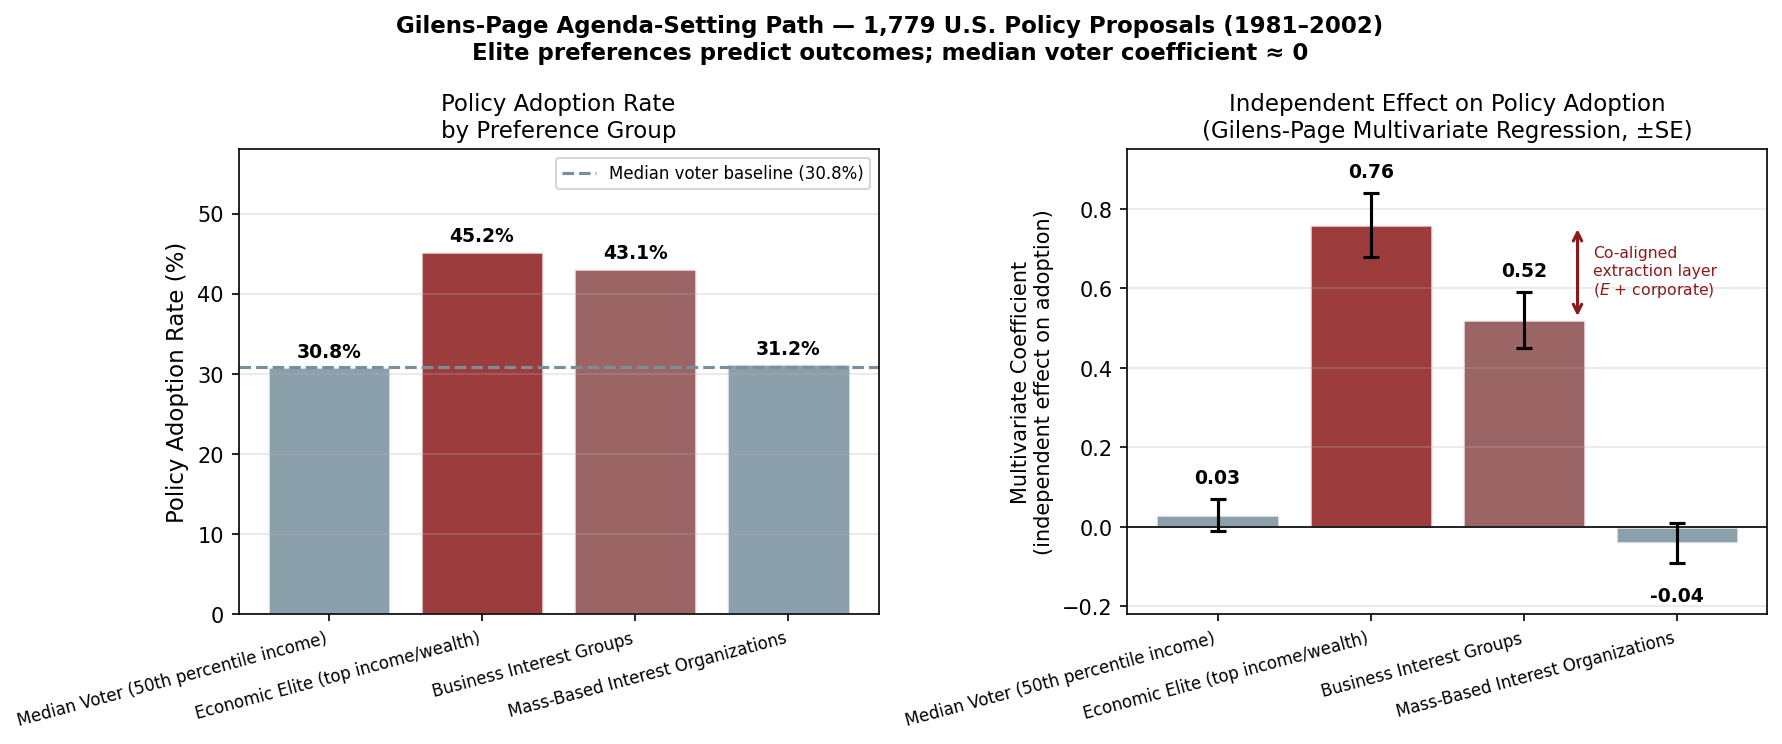
\includegraphics[width=0.92\textwidth]{figures/eq46_gilens_page.png}
  \caption{Gilens-Page (2014) results for 1,779 U.S.\ policy proposals (1981--2002). Left: policy adoption rate by preference group. Right: multivariate regression coefficients with standard-error bars (independent effect on adoption probability after controlling for other groups). The median voter coefficient ($0.03 \pm 0.04$, $p=0.43$) is statistically indistinguishable from zero; the economic elite coefficient ($0.76 \pm 0.08$, $p < 0.001$) and business interest group coefficient ($0.52 \pm 0.07$, $p < 0.001$) are both dominant --- and structurally co-aligned as components of $E$'s extraction layer. Mass-based organizations show a near-zero coefficient ($-0.04$), mirroring the median voter. This confirms eq.~\ref{eq:8.18-tweedism-agenda-path}: the agenda-setter routes $x_0 \rightarrow x_m$ to serve the full extraction layer ($E$ + organized corporate interests), leaving the median voter effectively powerless.}
  \label{fig:eq46_gilens}
\end{figure}

\paragraph{Comparison to prediction.}
Equation~\ref{eq:8.18-tweedism-agenda-path} predicts that the agenda-setter ($P_{\text{uppet}}$) sequences policy votes so that each step appears majority-winning while the terminal policy $x_m$ serves elite objectives. The Gilens-Page data confirm this: when economic elites support a policy, adoption probability rises significantly; when only the median voter supports it (elite opposed), adoption probability barely exceeds the no-support baseline. The business interest group finding deepens the confirmation: organized corporate lobbying and top-wealth individual preferences are statistically indistinguishable as predictors, jointly constituting the extraction layer's agenda-setting signal. The path $x_0 \rightarrow x_1 \rightarrow \cdots \rightarrow x_m$ is routed by the full weight of $E$ --- individual and corporate --- not by democratic aggregation.

\paragraph{Falsification criteria.}
This equation would be falsified if Gilens-Page analysis showed median voter preferences predicting policy outcomes as strongly as top-quintile preferences --- i.e., if the median voter coefficient were statistically indistinguishable from the elite coefficient in multivariate regression on the full 1,779-proposal dataset. The published results show the opposite across the full two-decade window and across multiple issue categories.

\paragraph{Confidence tier.}
\textbf{Tier~1.} Peer-reviewed dataset of 1,779 policy proposals over two decades; multivariate regression controls for cross-group preference overlap; results have been replicated by independent scholars using updated datasets; the core finding (near-zero median voter independent effect) is robust across methodological variations documented in the political science literature.

\subsection{The Decentralized Capital Threat: Bypassing the Tweedism Filter}

The mathematical vulnerability of the Tweedism Filter---and the most profound threat to Elite ($E$) control over the Puppet Class ($P_{\text{uppet}}$)---is the aggregation of decentralized capital. The ``Green Primary'' relies on the premise that only $E$ possesses the concentrated wealth necessary to fund a viable national campaign. However, the advent of digital crowdsourcing introduced a critical system anomaly: if millions of individuals within the Buffer Class ($I_{\text{buffer}}$) and the Out-group ($O_{\text{racialized}}$) aggregate micro-donations, they can mathematically exceed the funding power of $E$.

To stress-test whether this architecture persists beyond its formative era, we can observe a modern anomaly under contemporary electoral conditions.

The presidential campaigns of Senator Bernie Sanders in 2016 and 2020 served as a live stress test of this vulnerability. By refusing Elite capital and relying entirely on decentralized crowdsourcing, Sanders successfully bypassed the Tweedism Filter. He entered the upper echelons of the political interface not as a pre-approved member of $P_{\text{uppet}}$, but as an anomaly tethered directly to the working class. More dangerously, his platform explicitly targeted the extraction kernel: proposing wealth taxes on $E$ and universal healthcare, which would dismantle the engineered biological degradation and ``Affordability Trap'' detailed in Section~6.13.

\subsection{The Algorithmic Correction: Institutional Consolidation}

Because Sanders could not be neutralized through the standard financial filter (capital starvation), the Elite was forced to deploy the institutional apparatus of $P_{\text{uppet}}$ to execute an emergency algorithmic correction.

The political establishment and corporate media apparatus---both owned and operated by $E$---were activated to firewall the extraction kernel. In 2016, this manifested through internal institutional friction (as documented in the leaked DNC communications, which revealed active systemic bias to protect the pre-approved candidate). In 2020, the correction was executed with mathematical precision: observing that the decentralized threat was poised to win the primary plurality, the disparate approved members of $P_{\text{uppet}}$ executed a highly coordinated, unprecedented mass-suspension of their campaigns 48 hours before Super Tuesday. They consolidated their institutional weight behind a single, Elite-approved candidate to structurally block the anomaly. The system proved that when capital starvation fails, institutional collusion acts as the fail-safe.

\subsection{Political Capture and the Assimilation of the Anomaly}

The most insidious feature of the Predatory Min-Max Function is how it handles the anomaly after the threat has been blocked. The system prefers capture over kinetic destruction whenever possible, as destruction risks turning a populist leader into a martyr, thereby dropping the $Min$ variable (minimizing class resistance) to zero and sparking a revolt.

Instead, the system executed \textit{Political Capture}. Following his electoral defeat, Sanders was not exiled; he was absorbed. By granting him prestigious but mathematically contained roles within the interface---such as the Chairmanship of the Senate Budget Committee---the Elite transformed the anomaly into an institutional shield.

In exchange for these concessions, Sanders was required to endorse the approved $P_{\text{uppet}}$ interface, effectively acting as a sheepdog for his own revolutionary base. The Elite utilized his authentic credibility to pacify a highly mobilized, class-conscious coalition of $I_{\text{buffer}}$ and $O_{\text{racialized}}$, redirecting their kinetic energy back into the safe, pre-approved boundaries of the electoral system. The system successfully neutralized the decentralized capital threat by turning its architect into a load-bearing pillar of the very establishment he sought to dismantle.

\section{Empirical Validation: The Gilens--Page Study}
\label{sec:gilens_page}

The five-tier hierarchy is not merely theoretical---it has been empirically demonstrated at the level of national policy. Gilens and Page \cite{gilens} analyzed 1,779 policy issues over a twenty-year period, comparing the policy preferences of average citizens, economic elites, and organized interest groups against actual policy outcomes. Their findings are striking: the preferences of average citizens (corresponding to $I_{\text{buffer}}$, $F_{\text{enforce}}$, and $O_{\text{racialized}}$ in our model) had a ``near-zero, statistically non-significant impact upon public policy.'' By contrast, the preferences of economic elites (corresponding to $E$) had a substantial, statistically significant effect on which policies were adopted.

This result provides direct quantitative confirmation of the Predatory Min-Max Function. The system does not merely privilege $E$ in relative terms---it renders the policy preferences of everyone outside $E$ effectively irrelevant. When the preferences of average citizens diverge from those of economic elites, the citizens lose. When their preferences align, policy changes occur---but Gilens and Page show that this alignment, not citizen preference itself, drives the outcome. The mathematical implication is precise: the United States operates not as a majoritarian democracy but as what Gilens and Page term an ``economic-elite domination'' regime, in which $E$'s extraction objectives are translated into policy regardless of opposition from any tier below.

The psychological wage $\psi$ is not merely a side effect of the system; it is a \textit{designed feature}. The Elite ($E$) invest in $\psi$ precisely because it is cheaper than material concession: granting $I_{\text{buffer}}$ racial status, legal privileges over $O_{\text{racialized}}$, and the right to police the racial boundary costs the Elite far less than sharing material wealth. This makes $\psi$ the key variable in the Predatory Min-Max Function's minimization of class resistance (see Figure~\ref{fig:elite_model}). The system thus produces a paradox: $I_{\text{buffer}}$ defends a hierarchy that materially harms them, because the psychological wage creates the \textit{perception} of shared interest with $E$ and the \textit{perception} of threat from $O_{\text{racialized}}$. Both perceptions serve $E$'s extraction objectives. The psychological wage $\psi$ keeps the buffer class invested in a system that demonstrably excludes them from governance.

This is also the framework's answer to any analysis that treats globalization, technological disruption, or regulatory capture as alternative explanations for why the Puppet Class behaves as it does. External economic forces are not in competition with the Green Primary as causal accounts; they operate at different levels of the same causal chain. Globalization, automation, and financialization determine the content of what $E$ wants from the political system: trade liberalization, financial deregulation, offshoring-friendly tax policy, intellectual property expansion. The Green Primary and the Puppet Class filter determine whether $E$ obtains those policies \textit{regardless of whether the public agrees}. Gilens and Page's data confirm this directly: every major trade liberalization and financial deregulation of the 1981--2002 period occurred during the era of peak globalization and technological disruption, yet the dominant predictor of whether those policies passed was elite preference, not public pressure or competitive economic necessity. The same pattern applies to technological change: automation and platform monopolization are structural economic forces, but which industries receive regulatory protection, which workers receive retraining support, and which communities receive infrastructure investment are policy questions---and Gilens--Page confirms those questions are answered by $E$'s preferences, not citizens'. Non-racial economic forces explain what $E$ wants. The Puppet Class filter explains why $E$ gets it whether or not anyone else agrees. They are not competing explanations. They are the demand and the mechanism.

\section{The Mathematical Illusion of Democracy: The Agenda-Setter Trap}

When analyzing how the Elite ($E$) ensures that the democratic process never disrupts the extraction kernel, we must look beyond campaign finance (the Tweedism Filter) to the mathematical mechanics of voting itself. The Puppet Class ($P_{\text{uppet}}$) is entrusted with a critical function: they act as the ``Agenda Setter.''

In formal voting theory, an Agenda Setter does not need to explicitly force an electorate to vote against its own survival; they merely need to control the sequence of the votes. Majority preference over alternatives can be non-transitive: a population can prefer $x_A$ to $x_B$, $x_B$ to $x_C$, and still prefer $x_C$ to $x_A$ under distributed preference profiles. Once the Interference Engine has phase-shifted coalition timing, these cycles become exploitable.

By continuously pitting the marginal, short-term preferences of the Buffer Class ($I_{\text{buffer}}$) against the Out-group ($O_{\text{racialized}}$), the Agenda Setter fractures the electorate. $P_{\text{uppet}}$ presents a sequence of policy choices that offer temporary, localized gains---the material equivalents of the psychological wage ($\psi$)---while mathematically guaranteeing that the final, terminal policy adopted is the one that permanently protects Elite extraction. In policy-space terms, the setter advances from $x_0$ to $x_1,\ldots,x_m$ where each step wins a bare majority against the current baseline, even though the path as a whole drifts away from the cooperative class-optimal region.

Even if $I_{\text{buffer}}$ and $O_{\text{racialized}}$ collectively hold a supermajority that objectively opposes $E$'s interests, the Agenda-Setter trap ensures they can never effectively mobilize that majority. The electorate is mathematically defeated not by a lack of numbers, but by the sequential manipulation of their divided interests.
\section{Class Solidarity as the Algorithmic Antidote}

Mathematical models of sequential voting demonstrate only one viable countermeasure to an Agenda Setter: the fractured voting blocs must recognize the trap, cooperate, and actively agree to vote against their own immediate, marginal short-term gains in order to defeat the terminal policy.

This mathematical reality explains why systemic racism is not an incidental byproduct of the system, but an absolute structural necessity. The psychological wage of racism is a vital systemic firewall. By artificially engineering visceral, identity-based hatred and suspicion between $I_{\text{buffer}}$ and $O_{\text{racialized}}$, the Elite ensures that the cooperation required to defeat the Agenda Setter is psychologically impossible. As long as the Buffer Class views the Out-group as a greater existential threat than the Elite, the firewall holds, and the Agenda-Setter trap is permanently secured. Du Bois identified this precise dynamic in \textit{Black Reconstruction} \cite{dubois}: the defeat of Reconstruction-era cross-racial labor coalitions was accomplished not by superior military force but by the Elite's successful reinvestment of the psychological wage---convincing white workers that the gains they had made through multiracial Reconstruction governments were less valuable than the racial status hierarchy that replaced them. The ``Agenda-Setter trap'' is, in structural terms, the modern iteration of that same maneuver.
\section{Conditional Mobility and the ``New Money'' Anomaly}

A common counter-argument to systemic extraction models is the observable reality of class mobility---specifically, individuals from $O_{\text{racialized}}$ who achieve billionaire status and seemingly enter $E$. The framework must account for these anomalies.

Upward mobility from $O_{\text{racialized}}$ to $E$ is not a glitch in the system; it is a carefully managed feature we define as \textit{Conditional Assimilation}. When an individual from the Out-group acquires extreme capital, they are absorbed into a probationary tier of the Elite ($E_{\text{conditional}}$). However, this ascension is not accompanied by true, unrestrained autonomy.

Members of $E_{\text{conditional}}$ are permitted their wealth under strict, unwritten parameters: they may not use their capital or influence to dismantle the Predatory Min-Max Function. They are intensely surveilled by the institutional apparatus and are implicitly (or explicitly) threatened with rapid capital destruction if they step out of line.

More importantly, $E$ utilizes these individuals as high-visibility sociological tokens. By heavily publicizing their success, $E$ deploys the ideological narrative of the ``American Dream.'' This serves to pacify the Out-group by framing systemic extraction as a personal failure of work ethic, thereby reinforcing Component~4 of the oppressive architecture: the resistance to structural critique. The system allows a statistical fraction of $O_{\text{racialized}}$ to escape, precisely because doing so provides the ideological justification required to keep the rest of $O_{\text{racialized}}$ contained.

However, the most common pathway into $E_{\text{conditional}}$ is not passive tokenism; it is \textit{active service to the extraction kernel}. Conditional Assimilation is most readily granted when the ascending individual demonstrably compounds or exacerbates the system's effects upon their own demographic origin. The member of $E_{\text{conditional}}$ earns their probationary status by functioning as an ideological force multiplier---weaponizing their cultural credibility within $O_{\text{racialized}}$ to reinforce the very narratives that sustain extraction.

The transformation of hip-hop provides the definitive case study. In its foundational era (late 1970s--early 1990s), hip-hop functioned as a potent anti-authoritarian, class-conscious art form. Artists such as Public Enemy, KRS-One, and Tupac Shakur utilized the medium to articulate the mathematical realities of systemic extraction---police brutality, economic containment, and the carceral state---directly to the Out-group. Hip-hop was, in function, an organic resistance protocol: a cultural compiler translating the lived experience of $O_{\text{racialized}}$ into a politically mobilizing language that threatened to accelerate cross-class awareness.

The Elite's response was not censorship but \textit{capture}. Through the consolidation of record label ownership into a small number of corporate conglomerates controlled by $E$, the system executed a cultural Interface Swap. The distribution infrastructure was restructured to financially reward a specific, narrow content profile: the glorification of interpersonal violence within the Out-group, hyper-sexualization, conspicuous consumption of Elite-branded luxury goods, and the normalization of drug distribution---the very behaviors that feed the carceral pipeline. Anti-authoritarian, class-conscious content was not banned; it was simply \textit{defunded}. The algorithm of corporate promotion ensured that the dominant cultural output of hip-hop shifted from a diagnostic of systemic oppression to a promotional vehicle for self-destruction.

Members of $O_{\text{racialized}}$ who achieved extreme wealth through this captured medium---ascending into $E_{\text{conditional}}$---did so precisely because their cultural product \textit{served} the Predatory Min-Max Function. Their music conditioned the Out-group to internalize the trauma of extraction as aspirational identity, to view interpersonal violence as inevitable rather than engineered, and to direct collective energy toward individual consumption rather than structural critique. The system thus achieved a devastating efficiency: it converted the Out-group's primary resistance technology into a weapon aimed back at the Out-group itself, and it rewarded the operators of that weapon with conditional entry into the Elite.

\textbf{Algorithmic Correction: When New Capital Bypasses $E$'s Channels}

If the cultural capture of hip-hop illustrates how $E_{\text{conditional}}$ is \textit{granted} to those who serve the extraction kernel, the emergence of decentralized cryptocurrency reveals what happens when new capital is generated \textit{entirely outside} the Elite's controlled financial architecture. The system's response follows a two-phase protocol: first, attempted capture; if capture fails, destruction.

The 2026 release of Department of Justice files related to the Epstein network documented this capture protocol with striking precision. Jeffrey Epstein---whose network functioned as a control and blackmail apparatus for elements of $E$---invested approximately \$3~million in Coinbase's 2014 Series~C round and up to \$500,000 in Blockstream (a core Bitcoin infrastructure company). More critically, Epstein donated \$525,000 to MIT's Digital Currency Initiative (DCI), which absorbed three of the five core Bitcoin developers---including Lead Developer Wladimir van der Laan---just weeks after the Bitcoin Foundation filed for bankruptcy, creating a direct funding dependency between the open-source protocol's maintainers and a documented agent of Elite control. Epstein explicitly claimed to have ``spoken with some Bitcoin creators'' and attempted to meet Lead Maintainer Gavin Andresen as early as June 2011, months after Andresen assumed control from the pseudonymous Satoshi Nakamoto.

When outright capture proves insufficient---when decentralized capital threatens to create a parallel financial system beyond $E$'s jurisdictional reach---the system escalates to what the framework identifies as \textit{kinetic algorithmic correction}. Between 2018 and 2023, at least ten cryptocurrency founders and executives died under unusual circumstances. The temporal clustering is particularly striking: three died within approximately thirty days of each other during the November 2022 collapse of FTX---Nikolai Mushegian (MakerDAO co-founder, drowned October~28), Tiantian Kullander (Amber Group co-founder, died in his sleep at age~30 on November~23), and Vyacheslav Taran (Libertex Group, helicopter crash November~25). Mushegian's case is uniquely diagnostic: hours before his drowning in San Juan, Puerto Rico, he posted publicly that ``CIA and Mossad and pedo elite are running some kind of sex trafficking entrapment blackmail ring out of Puerto Rico and the Caribbean islands. They are going to frame me.'' Police reported no signs of foul play.

Whether these individual deaths represent coordinated elimination or statistical coincidence is, within the framework, less important than the \textit{systemic outcome}: decentralized capital that threatened to operate outside $E$'s extraction architecture was either absorbed into traditional financial channels (as when BlackRock launched its Bitcoin ETF post-FTX, completing the co-optation) or its controllers were neutralized. The pattern mirrors the two-track algorithm observed across every phase of the Predatory Min-Max Function: \textit{capture what can be captured; destroy what cannot}.

\subsection{The ``Socialism of Fools'' Anomaly: Misdirected Critique and the Shielding of $E$}

The systemic utility of the ``New Money'' anomaly relies on the Out-group member's strict adherence to the parameters of $E_{\text{conditional}}$. When an individual achieves extreme cultural and financial capital and attempts to bypass the ideological interface to critique the extraction kernel, the system's response depends entirely on the \textit{accuracy} of that critique.

The deplatforming and capital destruction of cultural figure Ye serves as a highly visible diagnostic of what occurs when a structural critique is fatally misdirected. Ye gestured at real critiques of elite power, media consolidation, and the role of ethno-religious state influence. However, rather than maintaining focus on the structural mechanics of extraction, he fell into what political theorists define as the ``socialism of fools''---redirecting a valid critique of state power and elite networks into generalized, conspiratorial blame against an entire identity group.

Within the mathematical framework of this book, this represents a critical targeting error. The anomaly correctly identified that the Elite ($E$) operates behind ideological shields, but he mistook the shield for the kernel itself. This misdirection is fatal to class solidarity and highly beneficial to the Elite for three structural reasons:

\begin{enumerate}
    \item \textbf{The Weaponization of Ideological Shields:} As contemporary structural analyses demonstrate, state power and elite interests routinely operate behind ideological, cultural, or religious shields. The issue is not the belief system itself, but how $P_{\text{uppet}}$ utilizes it to deflect criticism of elite behavior. By attacking the identity group rather than the class structure, the anomaly attacks the shield, leaving the Elite entirely untouched.

    \item \textbf{The Neutralization of Valid Critique:} Cases like the Epstein network (analyzed in Section~6.15) definitively prove that elite networks do engage in coordinated, systemic wrongdoing while successfully evading carceral accountability. However, when an anomaly like Ye uses broad bigotry to explain these power dynamics, it mathematically weakens the argument. It allows the system to permanently associate valid structural critiques of Elite power with toxic conspiracy theories, effectively discrediting the structural critique by association.

    \item \textbf{The Moral Justification for Annihilation:} Because the critique shifted into bigotry, it provided the corporate apparatus and $P_{\text{uppet}}$ with the unassailable moral high ground to execute a total quarantine. The systemic response---instantaneous debanking, severed corporate infrastructure, and the revocation of his $E_{\text{conditional}}$ status---was executed flawlessly under the banner of public safety and anti-hate. The Elite was able to annihilate a rogue billionaire and erase his capital without ever having to defend their actual structures of power.
\end{enumerate}

This event proves a fundamental theorem of the Predatory Min-Max Function: systemic critique must remain strictly focused on \textit{structures of power and class extraction}. The moment a critique shifts into blaming an entire demographic or identity group, it ceases to be a threat to the Elite and instead becomes a tool that ultimately protects the very systems being criticized.

\section{Algorithmic Corrections: The Intimidation of \texorpdfstring{$P_{\text{uppet}}$}{P\_uppet}}
\label{sec:legitimation_constraint}

What happens when the Tweedism Filter fails, and a member of $P_{\text{uppet}}$ attempts to assert actual autonomy? If a politician, a judge, or a foreign leader targets the extraction kernel, the system must execute an immediate ``algorithmic correction'' to bring the interface back into compliance.

These corrections scale based on the level of the threat. At the international level, when a member of a neocolonial Puppet Class---such as a Haitian president---demands economic reparations or attempts to nationalize resources, the correction often manifests as a kinetic assassination funded or facilitated by $E$.

Domestically, the corrections operate through institutional capture and targeted intimidation. For the highest echelons of the judicial branch, compliance is maintained through ``buybacks'' (e.g., undisclosed luxury travel and financial absorption by billionaires) that align the subjective interpretation of the law with Elite capital. Conversely, when judges issue rulings that threaten $E$'s agenda, the system deploys psychological terror: the targeted harassment of judicial families, violent threats, or the delivery of items (such as pizzas) to the private addresses of dissenting judges and their children. These acts serve as a stark, mafia-esque notification that $P_{\text{uppet}}$ is constantly surveilled. The Elite permits the Puppet Class to govern, but violently reminds them that they are entirely expendable.


\chapter{The Recompile: COINTELPRO, the Variable Swap, and the War on Drugs (1968--1994)}
\label{ch:recompile}

\begin{tcolorbox}[colback=black!5, colframe=black!70, fonttitle=\bfseries\ttfamily, title=RUNTIME LOG: 1968--1994 (THE RECOMPILE)]
\ttfamily\small
\textbf{System Stress} ($\min$: class resistance): \textcolor{red}{\textbf{CRITICAL}} --- Civil Rights Movement breached the legal interface. Demographic Paradox emerging: $O$ shrinking{,} extraction demand unchanged.\\
\textbf{Capital} ($\max$: extraction output): PEAK --- Carceral state fully industrialized. 13th Amendment loophole generating maximum throughput. War on Drugs providing unlimited proxy criminalization.\\
\textbf{Interference State} ($\Phi_{\text{load}}$, proximity to $\tau$): HIGH-DIMENSIONAL --- fractal identity routing active across multiple axes. Estimated $\Phi_{\text{load}} \in [0.75, 0.92]$, $\rho_{\tau} \in [0.80, 0.98]$.\\
\textbf{Variables Loaded}: ALL 5 TIERS --- $E$, $P_{\text{uppet}}$, $F_{\text{enforce}}$, $I_{\text{buffer}}$, $O_{\text{racialized}}$.\\
\textbf{Variables Deployed This Cycle}: $P_{\text{criminal}}$ (Variable Swap), $P_{\text{lead}}$ (Environmental Pre-Processing), $P_{\text{deindustrial}}$ (Economic Void), $P_{\text{BrokenWindows}}$ (Selective Enforcement), $P_{\text{retroactive}}$, $P_{\text{spatial}}$ (Gun-Free Zones), Universal Latent Criminality.\\
\textbf{Executing Function}: Full algorithm running. Variable Swap masks racial targeting. Demographic deficit forcing cannibalization of $I_{\text{buffer}}$.\\
\textbf{Policies Executed}: \textbf{[POLICY]} Anti-Drug Abuse Act (1986) --- 100:1 crack/powder ratio. \textbf{[POLICY]} Three Strikes laws. \textbf{[POLICY]} Assault Weapon Bans / Sensitive Place expansions. \textbf{[POLICY]} NFA tax increases / ex post facto serialization mandates.\\
\textbf{WARNING}: $\min$ VARIABLE FAILING. Buffer Class detecting contract breach. Kinetic calculus unfavorable. System entering terminal phase.
\end{tcolorbox}

\medskip

The reader has now watched the extraction algorithm being built, tier by tier, across four centuries: the Elite ($E$) and Out-group ($O_{\text{racialized}}$) in 15th-century Portugal, the Buffer Class ($I_{\text{buffer}}$) after Bacon's Rebellion, the Puppet Class ($P_{\text{uppet}}$) at the Constitutional Convention and its Gilded Age upgrade, and the Enforcement Class ($F_{\text{enforce}}$) through the slave patrol genealogy. This chapter traces the modern recompile: the counter-insurgency patch deployed after the 1954 \textit{Brown} kernel breach, the Variable Swap that replaced the explicit racial interface with race-neutral proxies, and the environmental and deindustrial preprocessing that generated the 1980s crime wave the Elite then cited to justify the 1994 Crime Bill. Chapter~\ref{ch:full_algo} takes up the algorithm's terminal runtime---the Demographic Paradox, the cannibalization of the Buffer Class, and the first full 5-Tier reveal. Chapter~\ref{ch:kinetic} returns to the kinetic variable that stands between the algorithm and its completion.

The recompile is where the fractal mind virus proves its polymorphism. Once explicit racial code became legally unstable, the payload moved into proxies that the host could defend as neutral: crime, disorder, drugs, school quality, property values, welfare dependency, neighborhood risk. The host no longer had to say ``race'' for the racial prior to execute. It only had to trust the new interface.

\section{The Source-Code Attack: Civil Rights Litigation as Kernel Breach}

Before we can understand the War on Drugs, we must first understand what \textit{forced} the Elite to execute the Variable Swap---because the system did not voluntarily abandon its explicit racial interface. It was \textit{broken} by a generation of brilliant legal architects from the racialized Out-group who did something the system was never designed to withstand: they read the source code.

A critical reframing is necessary here. Throughout this book, we have analyzed racism as a virus---an extraction algorithm parasitically embedded in the legal and economic infrastructure of the state. From the system's own perspective, any attempt to dismantle it registers as a threat, an intrusion. But we must ground our analysis in the moral reality: \textit{the system of racism is the virus}. The civil rights attorneys were not attackers; they were the immune response. They were citizens who understood that the only way to destroy a virus is to understand its architecture at the molecular level---and then target the source code, not the symptoms.

This is precisely what Thurgood Marshall, Charles Hamilton Houston, and the NAACP Legal Defense Fund executed across two decades of strategic litigation. Houston---Marshall's mentor at Howard University Law School---articulated the strategy with mathematical precision: he trained a generation of Black lawyers to be ``social engineers,'' to read the legal code not as a neutral system of justice but as the \textit{compiled output of the extraction algorithm}. Their approach was not to protest the interface (the ``Whites Only'' signs, the daily humiliations of Jim Crow) but to attack the kernel: the legal precedents that gave the algorithm its constitutional legitimacy.

The strategy was iterative and surgical. Beginning with \textit{Murray v.\ Pearson} (1936) and continuing through \textit{Sweatt v.\ Painter} (1950) and \textit{McLaurin v.\ Oklahoma} (1950), the NAACP Legal Defense Fund systematically dismantled the ``separate but equal'' doctrine established by \textit{Plessy v.\ Ferguson} (1896)---the legal patch the system had deployed to maintain racial extraction while claiming constitutional compliance. Each case was a targeted edit to the source code, exploiting the system's own internal contradictions: if ``separate but equal'' was the law, then the state had to \textit{actually provide} equal facilities, which the extraction kernel made economically impossible.

The culmination---\textit{Brown v.\ Board of Education} (1954)---was the most devastating kernel breach in the algorithm's history. By convincing the Supreme Court to unanimously strike down state-sanctioned segregation in public education, Marshall and his team did not merely change the interface; they invalidated the legal architecture that had sustained explicit racial extraction since the Virginia Slave Codes of 1705. For the first time in five centuries, the source code itself was edited by members of the Out-group.

The primary-trial record \cite{brown_v_board_record_1951}---now publicly accessible through the Internet Archive's 2026 release of 125,000 Supreme Court records and briefs \cite{ia_scotus_briefs_2026}---sharpens the framework's reading of this moment considerably. In the 1951 Kansas district court trial, sociologist Dr.\ Wilbur Brookover testified as an expert witness for the NAACP with a precision the framework recognizes as structural diagnosis rather than advocacy: ``In American society we consistently present to the child a model of democratic equality of opportunity\ldots At the same time, in a segregated school situation he is presented a contradictory or inharmonious model. He is presented a school situation in which it is obvious that he is a subordinate, inferior kind of a citizen\ldots the segregated schools perpetuate this conflict in expectancies, condemns the negro child to an ineffective role as a citizen and member of society.'' That testimony was entered as sworn evidence in 1951---three years before the Supreme Court acknowledged the psychological harm of segregation in its unanimous 1954 ruling. The evidentiary record had not changed between 1951 and 1954. What changed was the political calculus: the $C_{\text{legitimacy}}$ crisis created by Cold War competition with the Soviet Union, which made domestic racial apartheid an international liability the State Department was actively lobbying against \cite{dudziak}, shifted the cost-benefit analysis for the extraction kernel. The Court did not need to be persuaded that segregation produced inferior citizenship---that case had been made and entered into the record three years earlier. It needed to be persuaded that \textit{admitting} what had been proven was now strategically tolerable. The reform-absorption mechanism predicts exactly this: institutions do not respond to evidentiary sufficiency; they respond to the asymmetry between the cost of continued extraction and the cost of the marginal concession.

This is why the framework must not frame every reform as merely ``targeting the interface.'' The civil rights legal strategy \textit{did} reach the kernel. It \textit{did} alter the source code. The tragedy---and the proof of the system's adaptive resilience---is what happened next: the Elite immediately began recompiling.

\section{The Counterinsurgency Recompile: COINTELPRO (1956--1971)}
\label{sec:cointelpro_recompile}

Between the kernel breach of \textit{Brown} (1954) and the formal launch of the War on Drugs interface (1968), the state executed an intermediate control layer: domestic counterintelligence directed at lawful political organization. The FBI's COINTELPRO programs began in 1956 against the Communist Party and expanded into a multi-program architecture targeting Black liberation groups, anti-war and student organizers, Puerto Rican independence organizations, and, in a separate channel, white supremacist formations \cite{fbi_cointelpro_vault, fbi_new_left_vault, fbi_white_hate_vault}.

Within this framework, COINTELPRO is best modeled as a \textbf{counter-mobilization patch}. If Civil Rights litigation had edited constitutional source code, COINTELPRO attempted to degrade the social capacity needed to exploit that legal opening. Its function was not merely intelligence collection, but active disruption: break trust, fracture coalitions, isolate leaders, and increase the transaction costs of resistance.

\subsection{Program Architecture and Executive Logic}

The operational architecture of COINTELPRO was defined by a centralized, autocratic leadership model that insulated intelligence activities from external accountability. At the apex was Director J.\ Edgar Hoover, who cultivated an organizational culture where domestic intelligence needs were viewed as responsive to a ``higher law'' superseding statutory limitations and constitutional constraints \cite{fbi_cointelpro_vault}. Hoover issued the foundational directives to ``expose, disrupt, misdirect, discredit, or otherwise neutralize'' target groups, viewing systemic left-wing structural change as an existential threat to the state \cite{church_book2_1976}.

Beneath Hoover, the program was managed by a specific executive hierarchy that operationalized these directives:

\begin{table}[htbp]
\centering
\small
\caption{Executive Architecture of COINTELPRO}
\label{tab:cointelpro_executives}
\begin{tabular}{>{\raggedright}p{3cm} >{\raggedright}p{4cm} >{\raggedright\arraybackslash}p{7cm}}
\toprule
\textbf{Executive} & \textbf{FBI Role} & \textbf{Key Contribution to Architecture} \\
\midrule
J.\ Edgar Hoover & Director (1924--1972) & Primary architect; issued neutralization directives; insulated Bureau from oversight. \\
William C.\ Sullivan & Assistant Director & Managed day-to-day operations; authored memos identifying civil rights leaders (e.g., King) as paramount threats. \\
Mark Felt & Deputy Associate Director & Supervised compliance; authorized illegal operations including break-ins (later known as ``Deep Throat''). \\
Cartha D.\ DeLoach & Associate Director & Managed illicit media campaigns and selective leaks to sympathetic journalists. \\
John Matter & Audio Technician & Provided technical support for psychological warfare, including the preparation of blackmail tapes. \\
\bottomrule
\end{tabular}
\end{table}

This centralized command chain ensured that the program was not a series of scattered local excesses, but a top-down, meticulously orchestrated campaign to enforce the political status quo. The authorization occasionally intersected with the broader executive branch---such as Attorney General Robert F.\ Kennedy's narrow authorization for wiretapping Dr.\ King---but the FBI leveraged these openings to construct expansive, autonomous surveillance networks that far exceeded their original legal scope.

\paragraph{The domestic surveillance statute.}
The Wiretap Act---Title~III of the Omnibus Crime Control and Safe Streets Act of 1968---is codified at \usclink{apx:usc:18:2511}{18 U.S.C.~\S~2511}. Its operative prohibition nominally criminalizes unauthorized interception of communications, while its extensive exceptions provide the legal framework that COINTELPRO exploited (paired with the foreign-intelligence analogue at \usclink{apx:usc:50:1801abc}{50 U.S.C.~\S~1801} (FISA), already excerpted above):
\uscinline{usc_18_2511}

\subsection{Intelligence Apparatus: The Ghetto Informant Program (GIP)}

To facilitate the vast human intelligence requirements of the Black Nationalist track, the FBI established the Ghetto Informant Program (GIP), which operated from 1967 to 1973. This represented a dedicated civilian surveillance network designed to map the social and political contours of Black communities. Through the GIP, the FBI recruited and paid over 7,000 individuals---including postal workers, community organizers, and local business owners---to function as a panoptic surveillance layer.

One major deployment was Operation POCAM, which monitored the 1968 Poor People's Campaign. The GIP yield was staggering; a 1972 internal memorandum noted that the program produced an abundance of ``byproduct'' information on activities unrelated to civil unrest, leading to the reclassification of these informants into ``Security'' or ``Revolutionary Activities'' categories. This ensured that the surveillance infrastructure remained embedded in marginalized communities even after the formal program ended.

\subsection{Categorical Targets and the Asymmetry of Repression}
\begin{table}[htbp]
\centering
\small
\caption{COINTELPRO Program Clusters and Operational Logic}
\label{tab:cointelpro_clusters}
\begin{tabular}{>{\raggedright}p{2.5cm} >{\raggedright}p{4.5cm} >{\raggedright\arraybackslash}p{7cm}}
\toprule
\textbf{Program Cluster} & \textbf{Primary Targets} & \textbf{Operational Objective} \\
\midrule
Black Nationalist / Civil Rights & SCLC, BPP, SNCC, NOI. (Leaders: King, Malcolm X, Newton, Hampton, Carmichael). & Prevent the rise of a unified ``messiah''; absolute neutralization of leadership and coalition capacity. \\
The New Left & SDS, anti-war networks, student organizers (e.g., Nick Greer). & Restrict protest mobilization; create a repressive climate on campuses through interpersonal sabotage. \\
American Indian Movement (AIM) & AIM chapters, Pine Ridge Reservation supporters. & Militarized counter-insurgency; disrupt treaty protests and sovereignty claims via physical violence. \\
Puerto Rican Independence & MPJ, FUPI, Young Lords, FALN, Socialist Party. & Eviscerate anti-colonial mobilization; prevent internationalization of Puerto Rico's political status. \\
Communist / Socialist & CPUSA, SWP, socialist formations. & Blueprint for disruption (forgery, audits, media leaks); prevent labor-left coalition growth. \\
White Hate Groups & KKK, American Nazi Party, NSRP. & Manage and mitigate extreme violence without prioritizing ideological or institutional destruction. \\
\bottomrule
\end{tabular}
\end{table}

The program revealed a fundamental \textbf{asymmetry of repression}. While the FBI monitored white supremacist formations, the strategic posture was reactive: managing violence rather than seeking total neutralization. In contrast, the operations against the Black Panther Party, AIM, and the New Left were geared toward institutional eradication. For instance, of the 295 documented actions against Black Nationalist groups, 233 specifically targeted the Black Panther Party, seeking to permanently disable their community survival programs and self-defense infrastructure \cite{fbi_cointelpro_vault}.

At the center of this focus was Deputy Chairman Fred Hampton. Before his affiliation with the BPP, Hampton was a highly effective non-violent organizer, leading an NAACP youth council of over 500 members and successfully marching on Maywood Town Hall to secure an integrated public swimming pool \cite{hampton_bio}. His transition to revolutionary socialism was driven by the perceived limits of traditional civil rights frameworks in the face of entrenched systemic racism.

Hampton's most profound threat to the state was his success in forging the \textbf{Original Rainbow Coalition} (1969). This alliance systematically united disparate, marginalized groups across Chicago's segregated enclaves:
\begin{itemize}
    \item \textbf{The Young Lords Organization (YLO):} Led by Jos\'{e} ``Cha Cha'' Jim\'{e}nez, this Puerto Rican group transitioned from a street gang to a political organization fighting displacement and gentrification in Lincoln Park.
    \item \textbf{The Young Patriots Organization (YPO):} Comprised of poor, working-class Appalachian white migrants in Uptown who initially utilized the Confederate flag.
    \item \textbf{The Illinois Black Panther Party (ILBPP):} Provided the ideological and organizational core.
\end{itemize}
This coalition required intense ideological labor; Panther organizers like Bobby Lee played a crucial role in de-escalating racial tensions and demonstrating that the true enemy was not the racial other, but the capitalist power structure and its militarized police interface. By brokering non-aggression pacts among major street gangs and redirecting their energy toward survival programs---including free breakfasts and community health clinics operated by volunteers like Dr.\ Quentin Young---Hampton subverted the ``divide-and-conquer'' strategy that traditionally buttressed municipal and state power.

\subsection{Operational Doctrine: Infiltration, Psychological War, and Legal Burden}

The doctrine combined three mutually reinforcing vectors. First, \textbf{infiltration}: informants were used not only to report but to amplify internal suspicion, factional conflict, and strategic confusion. Second, \textbf{psychological warfare}: forged correspondence, anonymous messaging, reputational smears, and selective media seeding degraded trust both inside organizations and between movements and the public. Third, \textbf{legal-administrative pressure}: surveillance-fed prosecutions, repeated arrests, and procedural burdens consumed time, money, and leadership bandwidth \cite{church_book2_1976, fbi_cointelpro_vault}.

A central directive of this doctrine, issued in a March 4, 1968 memorandum, was to ``prevent the RISE OF A `MESSIAH' who could unify, and electrify, the militant black nationalist movement'' \cite{fbi_cointelpro_vault}. While the memo cited figures like Malcolm X and Dr.\ King, by 1969, Fred Hampton had clearly emerged as the Midwestern target of this designation.

The architectural linchpin of the operation against Hampton was William O'Neal, a paid informant handled by Special Agent Roy Martin Mitchell. O'Neal successfully infiltrated the BPP, eventually becoming Captain of Security. He functioned as an agent provocateur, pushing the organization toward criminality and even constructing an impromptu electric chair in BPP headquarters for intimidation purposes. Acting on Mitchell's directives, O'Neal provided a detailed floor plan of Hampton's apartment, mapping the exact location of his bed.

O'Neal's later \textit{Eyes on the Prize II} account confirms the control-edge logic from inside the operation: after walking through the Monroe Street apartment, he understood that the information he had supplied had facilitated the raid. The same broadcast transcript records that FBI headquarters authorized a \$300 bonus for his recent services \cite{eyes_on_prize_nation_law_transcript}. The evidentiary point is not psychological confession; it is the compensation structure. Informant access, spatial intelligence, and lethal police action were linked by a paid state feedback loop.

Crucially, strong forensic evidence indicates that O'Neal administered a massive dose of \textbf{secobarbital}---a powerful barbiturate---to Hampton during a late dinner on December 3, 1969. Independent toxicology screens by Dr.\ Eleanor Berman confirmed a comatose level of barbiturates in Hampton's bloodstream, rendering him unconscious before the state-sponsored assault began \cite{hampton_bio}.

The campaign against Dr.\ Martin Luther King Jr.\ remains one of the clearest documented examples of this doctrine. Congressional records describe warrantless or overbroad surveillance practices, weaponized personal intelligence, and the anonymous 1964 ``suicide package'' sent to King's home in an attempt at coercive neutralization \cite{church_book2_1976}. The core point is structural: private vulnerability became a state-managed control surface.

Tactical examples from this period demonstrate a systemic disregard for due process:
\begin{itemize}
    \item \textbf{Psychological Warfare and Reputational Sabotage:} The Bureau targeted actress Jean Seberg, a financial supporter of the Black Panthers, by planting a false story about her pregnancy to ``tarnish her image'' \cite{fbi_cointelpro_vault}. The resulting emotional trauma and premature birth of her child illustrated the Bureau's willingness to use personal catastrophe as a political tool.
    \item \textbf{Fomented Inter-Group Conflict:} Through forged correspondence and provocateurs, the Bureau deliberately instigated a lethal feud between the Black Panther Party and the US Organization (led by Ron Karenga). This artificially manufactured discord directly resulted in the assassinations of Panther members Alprentice ``Bunchy'' Carter and John Huggins.
    \item \textbf{Direct Kinetic Neutralization:} The 1969 assassination of Fred Hampton, the 21-year-old leader of the Chicago Black Panthers, provides the most extreme example. Hampton had successfully forged a multi-racial ``Rainbow Coalition'' of Black, Puerto Rican, and poor white youth. To destroy this alliance, FBI informant William O'Neal provided the Chicago Police Department with a detailed floor plan of Hampton's apartment. During a pre-dawn raid on December 4, 1969, a 14-man tactical unit detailed to Cook County State's Attorney Edward V.\ Hanrahan stormed the premises.

    The forensic record reveals a textbook case of disproportionate state violence. While Mark Clark was killed instantly in the front room, firing a single reflexive shot from his shotgun as he fell, the police unleashed a relentless fusillade of between 90 and 99 rounds into the small, four-room apartment. Hampton was lying in bed, deeply unconscious from the secobarbital, next to his pregnant fianc\'{e}e, Deborah Johnson. After Johnson was forcibly removed from the room, a chilling exchange was recorded between two officers inside Hampton's bedroom. After confirming he was ``barely alive'' following the initial volley, two point-blank gunshots rang out, followed by the casual report: ``He's good and dead now'' \cite{hampton_bio}.
\end{itemize}

In model terms, these tactics were not just individual acts of violence; they were \textbf{control vectors} designed to degrade the Out-group's organizational capacity and prevent cross-group solidarity.

Against the Black Panther Party and allied formations, COINTELPRO integrated intelligence penetration with local police operations, feeding both strategic disruption and kinetic risk at the street level \cite{fbi_cointelpro_vault, bloom2013}. In model terms, this was the same extraction kernel expressed through a policing-intelligence hybrid interface: preserve hierarchy by degrading autonomous organizational capacity in $O_{\text{racialized}}$ and preventing cross-group solidarity.

\subsection{Exposure, Oversight Shock, and Partial Reform}

COINTELPRO's secrecy was punctured on March 8, 1971, by a deliberate act of civilian civil disobedience. Under the moniker the ``Citizens' Commission to Investigate the FBI,'' a group of eight activists---including William C.\ Davidon, Bonnie and John Raines, and Keith Forsyth---successfully burgled the FBI's resident agency in Media, Pennsylvania \cite{medsger2014, aclu_davidon}.

The over 1,000 classified documents they retrieved provided a stark empirical breakdown of the Bureau's true institutional priorities:

\begin{table}[htbp]
\centering
\small
\caption{FBI Operational Focus (Media, PA Resident Agency, 1971)}
\label{tab:fbi_priorities}
\begin{tabular}{>{\raggedright}p{3cm} >{\centering}p{2cm} >{\raggedright\arraybackslash}p{8cm}}
\toprule
\textbf{Category} & \textbf{Percentage} & \textbf{Specific Focus} \\
\midrule
Political Surveillance & 40\% & Cases involving left-wing or liberal groups; merely 2 files concerning right-wing groups. \\
Serious Crimes & 15\% & Investigations into bank robberies, murder, rape, and interstate theft. \\
Draft Resistance & 14\% & Surveillance of military personnel leaving without permission and draft resisters. \\
Organized Crime & 1\% & Minor devotion to organized crime, primarily related to gambling. \\
Procedural Manuals & 30\% & Administrative matters and routine forms. \\
\bottomrule
\end{tabular}
\end{table}

The documents revealed that the FBI's primary function in the region was political suppression rather than crime-fighting. The exposure, lead-reported by Betty Medsger in the \textit{Washington Post}, forced the first public use of the acronym ``COINTELPRO'' and catalyzed the wave of investigations that followed.

The exposure catalyzed a wave of further legal and congressional actions. In 1972, NBC News correspondent Carl Stern Filed the first FOIA lawsuit to uncover the meaning of ``COINTELPRO--New Left,'' establishing a monumental precedent for judicial jurisdiction over intelligence matters.

The subsequent oversight shock produced real but incomplete guardrails. The Church Committee investigation (1975--1976), chaired by Senator Frank Church, documented systemic abuse and characterized the Bureau's activities as a ``sophisticated vigilante operation.'' This led to structural reforms:
\begin{itemize}
    \item \textbf{The Levi Guidelines (1976):} Attorney General Edward H.\ Levi issued regulations requiring a ``reasonable'' indication of criminal activity before initiating investigations, effectively prohibiting surveillance based solely on political rhetoric. The impact was immediate: the number of FBI domestic security investigations plummeted from over 21,000 in 1973 to 626 by September 1976 \cite{doj_oig_levi_guidelines}.
    \item \textbf{Informant Accountability:} The guidelines established a Suitability Review process for informants and mandated that the Bureau report unauthorized illegal activity by informants to the Department of Justice.
    \item \textbf{Legislative and Judicial Guardrails:} Senate Resolution 400 established the Senate Select Committee on Intelligence (SSCI) in 1976, and the Foreign Intelligence Surveillance Act (FISA) of 1978 inserted judicial review into national-security electronic surveillance \cite{sres400_1976, fisa_1978}.
\end{itemize}

\paragraph{Primary statutory text (FISA definitions, Title~50).}
The definitional scaffolding of FISA (Title~50, chapter~36) begins at \usclink{apx:usc:50:1801abc}{50 U.S.C.~\S~1801} (excerpt of subsections (a)--(c)):
\uscinline{usc_50_1801abc}

The civil aftermath was defined by a 13-year war of attrition in the federal courts: \textit{Hampton v.\ Hanrahan}. Represented by the People's Law Office (PLO), the survivors and families faced extreme judicial hostility from Judge Joseph Sam Perry, who initially dismissed the case and assessed punitive costs against the plaintiffs. However, a landmark 1979 decision by the Seventh Circuit reversed the dismissal, declaring that the plaintiffs had established a prima facie case of a multi-jurisdictional conspiracy to violate constitutional rights. This led to a historic \$1.85~million settlement in 1982, split equally among the City of Chicago, Cook County, and the federal government---a tripartite payment structure that served as a tacit admission of systemic conspiracy.

The political and legal legacy of the Hampton case reshaped Chicago. The electoral mobilization that defeated State's Attorney Hanrahan at the ballot box provided the organizational foundation for Harold Washington's 1983 election as the city's first Black mayor. Furthermore, the aggressive discovery and investigative model developed by the PLO during the litigation directly enabled the later exposure of the systemic torture ring operated by Chicago Police Commander Jon Burge. The psychological cost of the operation was equally profound: William O'Neal, the informant who facilitated the raid, died by suicide on January 15, 1990, the night his role was broadcast in the \textit{Eyes on the Prize II} documentary series.

\subsection{Modern Echoes: COINTELPRO 2.0?}

Despite the post-1971 reforms, the architectural framework of COINTELPRO continues to cast a long shadow over contemporary domestic intelligence. Civil liberties advocates frequently draw direct parallels to modern surveillance paradigms, such as the FBI's 2017 designation of ``Black Identity Extremists'' (BIE). This designation reflected a persistent institutional tendency to conflate radical political dissent and protests against police brutality with actionable domestic terrorism. Similarly, the legacy of the Ghetto Informant Program informs modern skepticism regarding massive federal surveillance networks, such as Operation TIPS (Terrorism Information and Prevention System), which sought to recruit civilian workers as domestic intelligence gatherers. These modern echoes suggest that while the interface of surveillance has updated, the underlying logic of domestic pacification remains a core function of the extraction architecture.

\subsection{Transition to the Variable Swap}

COINTELPRO therefore marks a crucial bridge in the book's chronology. Explicit racial code had been legally destabilized, but mass democratic mobilization still threatened the extraction architecture. The state response was two-step: first, counterintelligence disruption of movement infrastructure (COINTELPRO); second, migration to administratively ``neutral'' criminal proxies (the War on Drugs and the broader law-and-order stack). Put differently, COINTELPRO was the emergency containment patch; the War on Drugs was the scalable long-run recompile.

\section{The Interface Shift: The War on Drugs (1968)}

\begin{tcolorbox}[colback=black!5, colframe=black!70, fonttitle=\bfseries\ttfamily, title=RUNTIME LOG: 1966 (SECURITY PATCH)]
\ttfamily\small
\textbf{System Stress} ($\min$: class resistance): CRITICAL --- Civil Rights Movement breaches the legal kernel (\textit{Brown v. Board}). Cognitive Field Independence spike detected via IFAS Protocol (91\% breakthrough rate). Subjects visualizing the extraction architecture.\\
\textbf{Capital} ($\max$: extraction output): THREATENED --- Legal desegregation disrupts existing labor and housing extraction models ($P_{\text{redlining}}$).\\
\textbf{Interference State} ($\Phi_{\text{load}}$, proximity to $\tau$): HIGH. Cross-racial solidarity (Black Power + Anti-War) increasing $\min$. $\rho_{\tau}=M(t)/\tau \rightarrow 0.95$.\\
\textbf{Active Patch}: Executing 1966 Moratorium. Revoking IND exemptions for normal human subjects. Shutting down IFAS mid-session. California Schedule I: LSD (Oct.\ 1966). Federal Drug Abuse Control Amendments (1968). Controlled Substances Act completes scheduling architecture (1970). Recompiling Version 2.0 (The Variable Swap).\\
\textbf{Variables Deployed}: $P_{\text{criminal}}$ (Proxy variable for race), $P_{\text{spatial}}$ (Proxy for neighborhood).\\
\textbf{Result}: Epistemic Enclosure restored. Cognitive Field Independence suppressed. Extraction Algorithm migrated to race-neutral interface (The War on Drugs).
\end{tcolorbox}

Before examining the Variable Swap itself, it is essential to understand its prototype. The transposition of substance use from the medical domain into the carceral domain did not begin with Richard Nixon; it was a strategic project with roots decades earlier, and its template reveals the algorithmic logic with crystalline clarity.

The opening salvo was the \textbf{Marihuana Tax Act of 1937}, orchestrated by Federal Bureau of Narcotics Commissioner Harry J.\ Anslinger. Cannabis had resided in the United States Pharmacopeia as a recognized medical tincture since 1850; Anslinger exploited anti-Mexican and anti-Black sentiment to reclassify it from medicine into contraband \cite{bonnie}. His rhetoric was explicitly racialized: he associated marijuana with Mexican immigrants and Black jazz musicians, fabricating lurid narratives of drug-induced violence to manufacture the public consent necessary for criminalization. Following the 1937 Act, cannabis was not officially removed from the Pharmacopeia until 1941---the deliberate lag illustrating the sheer institutional effort required to strip a substance of its medical legitimacy in order to activate its carceral utility.

The template Anslinger established is the precise logic the extraction kernel requires: criminalize a substance not on the basis of scientific evidence, but to enable the surveillance and disruption of specific demographic groups within $O_{\text{racialized}}$. This template was refined and scaled by every subsequent administration. When the civil rights attorneys breached the kernel (see Section~6.1), the system already possessed a proven mechanism for recriminalizing the Out-group without naming race.

Because the civil rights attorneys had breached the kernel---invalidating the explicit racial code that had sustained extraction since 1705---the Nixon Administration was forced to execute the \textbf{Variable Swap} (see Figure~\ref{fig:variable_swap}). As John Ehrlichman admitted, they used the \textbf{War on Drugs} to associate ``blacks with heroin'' and ``hippies with marijuana'' \cite{baum, vera, alexander, webb}.

This expanded the Out-group to include political dissidents from the In-group, while Lee Atwater's \textbf{``Dog Whistle''} strategy (1981) provided the abstract language (``State's Rights,'' ``Law and Order'') to mask the operation from the white public \cite{lopez, phillips}.

The crack-versus-powder cocaine sentencing disparity is perhaps the single most elegant proof that the War on Drugs was an engineered racial targeting system, not a public health initiative. The Anti-Drug Abuse Act of 1986 established a \textbf{100-to-1 sentencing ratio}: possession of 5 grams of crack cocaine---the form disproportionately associated with Black urban communities---triggered the same mandatory five-year federal minimum sentence as possession of 500 grams of powder cocaine---the form associated with affluent white users \cite{alexander}. Pharmacologically, crack and powder cocaine are \textit{the same molecule}. The difference is the delivery mechanism, not the substance. Yet the system encoded a hundredfold sentencing asymmetry along precisely the racial fault line the Variable Swap required. The disparity was not an oversight; it was the extraction kernel expressing itself through the ``race-neutral'' interface of drug scheduling. When Congress finally reduced the ratio to 18-to-1 with the Fair Sentencing Act of 2010, it did so \textit{without retroactive relief}---leaving tens of thousands of Black citizens to serve out sentences that Congress itself had acknowledged were unjust. The system updated its interface while leaving the existing extraction intact.

\begin{figure}[htbp]
\centering
\begin{tikzpicture}[
    shell/.style={draw, thick, rounded corners=4pt, minimum height=1.0cm, align=center, font=\small},
    arr/.style={->, thick, >=stealth},
    scale=0.88, transform shape
]
    % Interface layers (stacked, oldest at bottom nearest kernel)
    \node[shell, fill=red!25, minimum width=10.5cm] (i1) at (0,2.0) {\textbf{Interface 1} (pre-1865): $\text{Race}(x) = \text{Black} \rightarrow \text{Target}$};
    \node[shell, fill=orange!25, minimum width=10.5cm] (i2) at (0,3.3) {\textbf{Interface 2} (post-1865): $\text{Status}(x) = \text{Criminal} \rightarrow \text{Target}$};
    \node[shell, fill=yellow!30, minimum width=10.5cm] (i3) at (0,4.6) {\textbf{Interface 3} (post-1968): $\text{Association}(x) = \text{Drug User} \rightarrow \text{Target}$};
    \node[shell, fill=purple!20, minimum width=10.5cm] (i4) at (0,5.9) {\textbf{Interface 4} (present): $\text{Anyone} \rightarrow \text{Target}$ via selective enforcement};

    % Single funnel arrow from interface stack to kernel
    \draw[->, very thick, black!50] (0,1.45) -- (0,0.85);
    \node[font=\tiny\bfseries, black!50, anchor=west] at (0.2,1.15) {any one active at a time};

    % Kernel (below)
    \node[shell, fill=black!15, minimum width=10.5cm, minimum height=1.4cm, font=\small\bfseries] (kernel) at (0,0) {KERNEL (unchanged since 1450s)\\{\normalfont\footnotesize $\text{Status}(x) \in \text{Target} \rightarrow \text{Uncompensated Labor / Extraction}$}};

    % Right-side era labels
    \node[font=\tiny, gray, anchor=west] at (5.6,2.0) {Chattel slavery};
    \node[font=\tiny, gray, anchor=west] at (5.6,3.3) {13th Amend.\ + Black Codes};
    \node[font=\tiny, gray, anchor=west] at (5.6,4.6) {War on Drugs};
    \node[font=\tiny, gray, anchor=west] at (5.6,5.9) {Universal criminality};

    % Left-side bracket and label for interfaces
    \draw[thick, black, decorate, decoration={brace, amplitude=6pt, mirror}] (-6.2,1.5) -- (-6.2,6.4);
    \node[font=\footnotesize, black, rotate=90] at (-6.9,3.9) {INTERFACE (swappable)};

    % Left-side bracket and label for kernel
    \draw[thick, black, decorate, decoration={brace, amplitude=6pt, mirror}] (-6.2,-0.75) -- (-6.2,0.75);
    \node[font=\footnotesize, black, rotate=90] at (-6.9,0) {KERNEL (fixed)};

    % Bottom annotation
    \node[font=\scriptsize, align=center, gray] at (0,-1.4) {What appears as ``progress'' (abolition, civil rights) is an interface update.\\The extraction kernel has never been modified.};
\end{tikzpicture}
\caption{\textbf{The Variable Swap: Interface vs.\ Kernel.} The system's extraction function (kernel) remains constant across all eras. Only the \textit{input variable}---the mechanism by which targets are selected---changes. Each historical ``reform'' swaps the interface (from explicit race to criminal status to drug association to universal latent criminality) while leaving the kernel intact. The appearance of progress masks functional continuity.}
\label{fig:variable_swap}
\end{figure}

\subsection{Epistemic Hypocrisy: Patent 6,630,507 and the Carceral Annihilation of Tameka Drummer}

To understand the sheer malice of the $P_{\text{criminal}}$ proxy variable during the War on Drugs, one must examine the system's epistemic hypocrisy---the reality that the Elite ($E$) possesses the scientific truth of a substance, monopolizes its intellectual property, and yet legally mandates the exact opposite reality to justify the extraction kernel.

The federal government maintains cannabis as a Schedule~I controlled substance, legally defined as having ``no currently accepted medical use and a high potential for abuse.'' The operative scheduling criteria and the prohibition they activate appear at \usclink{apx:usc:21:812b}{21 U.S.C.~\S~812(b)} and \usclink{apx:usc:21:841a}{21 U.S.C.~\S~841(a)}:
\uscinline{usc_21_812b}
\uscinline{usc_21_841a}
This classification is the load-bearing pillar of the modern carceral state, providing the Enforcement Class ($F_{\text{enforce}}$) with the legal authorization to invade, arrest, and cage millions of Out-group citizens.

Yet, the state's own internal archives prove this classification is a deliberate, manufactured lie. On October 7, 2003, the United States Patent and Trademark Office granted U.S.\ Patent 6,630,507, titled ``Cannabinoids as antioxidants and neuroprotectants.'' The official assignee of this patent is \textit{the United States of America}, as represented by the Department of Health and Human Services (HHS).

Mathematically, the state engineered a strict binary:

\begin{itemize}
    \item \textbf{For the Elite ($E$):} Cannabis is recognized as a profound neuroprotectant and antioxidant, and its biochemical properties are patented as intellectual property to secure future pharmaceutical capital.

    \item \textbf{For the Out-group ($O$):} Cannabis is classified as a highly dangerous narcotic, serving strictly as the $P_{\text{criminal}}$ variable to strip constitutional autonomy and funnel bodies into the 13th Amendment loophole.
\end{itemize}

The human cost of this algorithmic duality is absolute. We need look no further than the physical reality of Tameka Drummer (MDOC Inmate \#138477). In 2008, following a routine traffic stop for an expired license plate, police found less than two ounces of cannabis in her vehicle. Because Mississippi operates under draconian ``habitual offender'' laws, this minor possession charge triggered a mandatory maximum enhancement based on past convictions for which she had already served her time.

For possessing a minuscule amount of a plant that the federal government officially holds the medical patent for, Tameka Drummer was sentenced to \textbf{life in prison without the possibility of parole}. As of 2026, she remains caged at the Central Mississippi Correctional Facility.

Her life sentence mathematically proves that the War on Drugs has absolutely nothing to do with public health or the inherent danger of a substance. The Elite knows the plant is medicine; they patented it. They simply play ignorant because admitting the truth would dismantle the primary proxy variable they use to execute the systemic culling and carceral extraction of the Out-group. Tameka Drummer is not serving life for a drug crime; she is serving life because the Predatory Min-Max Function requires a constant stream of biological assets, and the state will maintain a lethal fiction to ensure the cages stay full.

\section{The Manufactured Crisis: Environmental Poisoning, Deindustrialization, and the Algorithmic Input}

The War on Drugs gave the Elite its proxy variable. But a proxy variable is useless without \textit{input data}---without a measurable surge in violence that the system could point to as justification for expanding the carceral apparatus. This section demonstrates that the input data was not organic; it was \textbf{manufactured} by a confluence of environmental poisoning, economic demolition, and market dynamics---all concentrated, with mathematical precision, in the communities already marked by the compounding chain formalized in Section~4.5.

\subsection{The Empirical Topography: Quantifying the Surge}

Between the early 1960s and the mid-1990s, the United States experienced an unprecedented escalation in violent crime. The FBI's Uniform Crime Reporting (UCR) program and the Bureau of Justice Statistics' National Crime Victimization Survey (NCVS) together document a stark trajectory: in 1960, the national homicide rate stood at 5.1 per 100,000 population, with an estimated 9,110 homicides nationwide. Over the next two decades, this rate \textbf{doubled}, peaking at 10.2 per 100,000 in 1980 (23,040 deaths). Following a brief recession, it surged again to 9.8 per 100,000 in 1991 (24,703 homicides). The overall violent crime rate---murder, rape, robbery, and aggravated assault---\textbf{more than tripled} between 1960 and 1991 \cite{ucr_historical, bjs_ncvs}.

\begin{table}[htbp]
\centering
\small
\caption{U.S.\ Homicide and Violent Crime Trajectory, 1960--1999}
\label{tab:crime_surge}
\begin{tabular}{lrrrr}
\toprule
\textbf{Year} & \textbf{Population} & \textbf{Homicides} & \textbf{Rate/100k} & \textbf{Violent Crimes} \\
\midrule
1960 & 179,323,175 & 9,110 & 5.1 & 288,460 \\
1970 & 203,265,212 & 16,000 & 7.9 & 738,820 \\
1980 & 225,349,264 & 23,040 & 10.2 & 1,344,520 \\
1991 & 252,177,000 & 24,703 & 9.8 & 1,911,770 \\
1999 & 272,690,813 & 15,522 & 5.7 & 1,426,044 \\
\bottomrule
\end{tabular}
\end{table}

A critical transition during this era was the changing topology of violence. Historically, homicide was predominantly interpersonal---committed among acquaintances or domestic partners. During the 1970s and 1980s, stranger homicides increased much faster than domestic killings, and robberies escalated by a factor of four between 1960 and 1980. This shift toward impersonal, unpredictable violence in public spaces generated an unprecedented level of national fear---precisely the political raw material the Elite required to justify the carceral expansion.

\begin{figure}[htbp]
\centering
\begin{tikzpicture}
\begin{axis}[
    width=0.95\textwidth,
    height=9cm,
    xlabel={Year},
    ylabel={Rate per 100{,}000 Population},
    title={\textbf{U.S. Homicide Rate and Firearm Homicide Rate, 1960--1999}},
    xmin=1958, xmax=2001,
    ymin=0, ymax=12,
    xtick={1960,1965,1970,1975,1980,1985,1991,1995,1999},
    xticklabel style={rotate=45, anchor=east, font=\small, /pgf/number format/1000 sep={}},
    ytick={0,2,4,6,8,10,12},
    grid=major,
    grid style={dashed, gray!40},
    mark size=3pt,
    every axis title/.style={font=\bfseries\small, at={(0.5,1.05)}},
    legend style={at={(0.02,0.98)}, anchor=north west, font=\small},
]
\addplot[thick, blue!70!black, mark=*] coordinates {
    (1960, 5.1) (1965, 5.1) (1970, 7.9) (1975, 9.6)
    (1980, 10.2) (1985, 7.9) (1991, 9.8) (1995, 8.2) (1999, 5.7)
};
\addlegendentry{Total Homicide Rate}
\addplot[thick, red!70!black, mark=diamond*, densely dashed] coordinates {
    (1960, 2.6) (1965, 2.8) (1970, 4.8) (1975, 6.3)
    (1980, 6.9) (1985, 4.8) (1991, 7.1) (1995, 5.5) (1999, 3.8)
};
\addlegendentry{Firearm Homicide Rate}
\node[above right, font=\scriptsize, blue!60!black] at (axis cs:1980,10.2) {\textbf{10.2}};
\node[above right, font=\scriptsize, blue!60!black] at (axis cs:1991,9.8) {\textbf{9.8}};
\draw[densely dotted, olive!80!black] (axis cs:1968,0) -- (axis cs:1968,12);
\node[rotate=90, anchor=south, font=\tiny, olive!80!black, fill=white, inner sep=1pt] at (axis cs:1968,6) {Gun Control Act (1968)};
\draw[densely dotted, olive!80!black] (axis cs:1971,0) -- (axis cs:1971,12);
\node[rotate=90, anchor=south, font=\tiny, olive!80!black, fill=white, inner sep=1pt] at (axis cs:1971,6) {War on Drugs (1971)};
\draw[densely dotted, purple!70!black] (axis cs:1986,0) -- (axis cs:1986,12);
\node[rotate=90, anchor=south, font=\tiny, purple!70!black, fill=white, inner sep=1pt] at (axis cs:1986,6) {Anti-Drug Abuse Act (1986)};
\draw[densely dotted, red!60!black] (axis cs:1994.5,0) -- (axis cs:1994.5,12);
\node[rotate=90, anchor=south, font=\tiny, red!60!black, fill=white, inner sep=1pt] at (axis cs:1994.5,6) {1994 Crime Bill};
\end{axis}
\end{tikzpicture}
\caption{\textbf{The Empirical Input: Homicide Rate Trajectory, 1960--1999.} The homicide rate doubled between 1960 and 1980, providing the ``crisis data'' the carceral algorithm required. Firearm homicides consistently accounted for 60--70\% of all homicides, peaking at approximately 70\% in 1991. Policy event markers show the legislative responses---each one expanding the extraction kernel's reach. Sources: FBI UCR; BJS Supplementary Homicide Reports; CDC WONDER.}
\label{fig:homicide_surge}
\end{figure}

\subsection{The Toxin Pre-Processor: Environmental Lead as \texorpdfstring{$P_{\text{lead}}$}{P\_lead}}

\textbf{Methodological note: population-level causation vs.\ individual moral responsibility.}
The analysis that follows operates at the level of \textbf{population epidemiology}, not individual psychology. It identifies the distributional effect of a policy variable---$P_{\text{lead}}$, the deliberate and then deliberately concealed mass deployment of a neurotoxin---on the aggregate behavioral profile of entire cohorts of children across a 20-year developmental window. Epidemiological causation of this kind does not require, and does not make, any claim about the intentions, choices, or moral standing of any individual person. The statement ``lead exposure elevated population-level violent crime rates by 0.8 elasticity'' is a distributional fact about a cohort. It is not a statement about any member of that cohort.

This distinction is not semantic. It is the same methodological boundary the Preface establishes between \textit{architecture} and \textit{phenomenology}: this framework analyzes the design of the system, not the lived experience or moral character of those inside it. The framework locates culpability precisely at the level of the corporate and governmental actors who constituted $P_{\text{epistemic}}$---the Ethyl Corporation, General Motors, Standard Oil, and the federal regulatory apparatus they captured---who possessed proof of mass neurological harm by 1924, suppressed it for 70 years, and used that suppression to ensure the neurotoxin continued compounding onto the same populations already depleted by the preceding extraction chain. The moral responsibility runs \textit{upstream}, to those actors. It does not dissolve the responsibility of anyone who harmed another person; it adds, in parallel, the responsibility of those who \textit{engineered the conditions} in which harm became statistically predictable.

The predictable misreading---``this framework says lead made them do it and therefore no one is responsible''---inverts the actual claim. The framework says that identifiable actors \textit{knowingly manufactured a biological condition} that impaired impulse regulation across millions of children in a targeted geographic pattern, and that the subsequent violence was the predictable statistical output of those upstream decisions. Every individual who harmed someone bears responsibility for that harm. So does every corporate officer who signed a memo suppressing the neuroscience. The distinction between these two levels of responsibility is not a contradiction; it is a \textit{necessary} analytical separation that the traditional individual-prejudice model of racism refuses to make.

While the War on Drugs provided the legal mechanism and the empirical surge provided the political justification, the question remains: what \textit{caused} the surge itself? Traditional criminological frameworks---social disorganization theory (the Chicago School), strain theory (Merton), and routine activities theory (Cohen and Felson)---explain the broad behavioral context of crime under structural pressure. But they struggle to account for the precise \textit{timing} and the sheer biological \textit{magnitude} of the surge across varied geographic typologies. This analytical gap is filled by environmental epidemiology: the \textbf{lead-crime hypothesis}.

This hypothesis posits that the drastic rise in violent crime between 1960 and 1990 was fundamentally driven by the ubiquitous exposure of young children to neurotoxic environmental lead. The primary vector was the combustion of tetraethyllead in motor vehicle gasoline, supplemented by the deterioration of lead-based paint in aging inner-city housing and lead water service lines. Lead is a severe neurotoxin that penetrates the blood-brain barrier. Extensive biological and epidemiological research demonstrates that early childhood lead exposure permanently damages the brain's prefrontal cortex, heavily impairing executive functions---resulting in lowered IQ, attention deficit hyperactivity disorder, heightened impulsivity, unchecked aggression, and an inability to regulate behavioral responses \cite{reyes2007, nevin2007}.

The epidemiological data aligns with striking precision. Leaded gasoline consumption rose steadily from the 1940s through the early 1970s, dispersing millions of tons of lead dust into the soil and air---particularly near the dense urban traffic corridors that ran directly through redlined neighborhoods (see Section~4.8). Because peak criminal offending universally occurs in young adulthood (late teens to early twenties), the hypothesis dictates a roughly \textbf{20-year lag} between peak biological exposure and peak criminal activity. The generation born into the most heavily lead-polluted environments of the late 1960s and early 1970s reached their peak offending years in the late 1980s and early 1990s---\textit{perfectly mirroring the crest of the violent crime surge}.

Economist Jessica Wolpaw Reyes utilized the state-by-state phase-out of leaded gasoline under the Clean Air Act as a natural experiment. Because the regulations were implemented at different rates across different states, Reyes was able to isolate the variable, finding a remarkably high \textbf{elasticity of 0.8} between lead and violent crime: a 10\% increase in lead exposure correlated with an 8\% increase in violent crime \cite{reyes2007}. Research by Anna Aizer and Janet Currie in Rhode Island demonstrated that localized childhood lead exposure substantially increased school suspensions and juvenile detention rates \cite{aizer_currie}. Historical data reveals that cities utilizing lead water pipes in the early 20th century experienced homicide rates \textbf{24\% higher} than cities using iron pipes, particularly in areas with acidic water that leached the neurotoxin. A comprehensive 2022 meta-analysis by Higney, Hanley, and Moro consolidated findings from 24 independent studies, confirming substantial evidence linking lead exposure to a heightened risk of criminal behavior \cite{higney2022}.

Within the framework of this book, environmental lead exposure functions as an additional policy variable, $P_{\text{lead}}$, applied to the compounding model of Section~4.5:
\begin{equation}\label{eq:9.1-lead-crime-compounding}
O_{t+1}^{\text{capacity}} = O_t^{\text{capacity}} \cdot (1 - \alpha_{P_{\text{lead}}})
\end{equation}
The critical insight is that $P_{\text{lead}}$ was not applied uniformly. Because leaded gasoline exhaust concentrated along highway corridors, and because those corridors were deliberately routed through redlined neighborhoods (see Section~4.8), and because deteriorating lead paint accumulated in the disinvested housing stock of those same neighborhoods, the neurotoxin was concentrated onto the Out-group already diminished by the compounding chain: slavery $\rightarrow$ Black Codes $\rightarrow$ convict leasing $\rightarrow$ redlining. In the framework's theoretical vocabulary, the lead-crime hypothesis does not merely explain the timing of the surge; it reveals the surge as another iteration of the extraction algorithm's compounding function, operating through biological channels.

\begin{figure}[htbp]
\centering
\begin{tikzpicture}
\begin{axis}[
    width=0.95\textwidth,
    height=9.5cm,
    title={\textbf{Lead Exposure (Shifted +22 Years) vs.\ Violent Crime and Firearm Homicide}},
    xlabel={Year (Crime Data Timeline)},
    ylabel={Rate per 100{,}000 (Crime)},
    axis y line*=left,
    xmin=1960, xmax=2020,
    enlarge x limits={0.04, 0.01},
    ymin=0, ymax=800,
    xtick={1960,1965,1970,1975,1980,1985,1990,1995,2000,2010,2015},
    xticklabel style={rotate=45, anchor=east, font=\small, /pgf/number format/1000 sep={}},
    grid=major,
    grid style={dashed, gray!40},
    ylabel style={blue!70!black, yshift=10pt},
    mark size=2pt,
    every axis title/.style={font=\bfseries\small, at={(0.5,1.05)}},
    legend style={at={(0.02,0.98)}, anchor=north west, font=\small},
]
\addplot[thick, blue!70!black, mark=*] coordinates {
    (1960, 161) (1963, 168) (1966, 220) (1969, 328)
    (1972, 401) (1975, 488) (1978, 497) (1980, 597)
    (1982, 571) (1985, 557) (1988, 637) (1990, 730)
    (1991, 758) (1993, 747) (1995, 685) (1997, 611)
    (2000, 507) (2002, 494)
    (2010, 403.6) (2011, 387.1) (2012, 387.8) (2013, 369.1) (2014, 361.6) (2015, 373.7)
};
\addlegendentry{Violent Crime Rate}
\addplot[thick, orange!80!black, mark=diamond*, densely dashed] coordinates {
    (1960, 26) (1963, 27) (1966, 33) (1969, 42)
    (1972, 52) (1975, 63) (1978, 60) (1980, 69)
    (1982, 58) (1985, 48) (1988, 55) (1990, 70)
    (1991, 71) (1993, 71) (1995, 55) (1997, 44)
    (2000, 38) (2002, 36)
    (2010, 36) (2011, 36) (2012, 38) (2013, 35) (2014, 35) (2015, 40)
};
\addlegendentry{Firearm Homicide Rate ($\times$10)}
\draw[densely dotted, teal!80!black] (axis cs:1970,0) -- (axis cs:1970,800);
\node[rotate=90, anchor=south, font=\tiny, teal!80!black, fill=white, inner sep=1pt] at (axis cs:1970,400) {Clean Air Act (1970)};
\draw[densely dotted, teal!80!black] (axis cs:1973,0) -- (axis cs:1973,800);
\node[rotate=90, anchor=south, font=\tiny, teal!80!black, fill=white, inner sep=1pt] at (axis cs:1973,400) {EPA lead phaseout (1973)};
\draw[densely dotted, purple!70!black] (axis cs:1986,0) -- (axis cs:1986,800);
\node[rotate=90, anchor=south, font=\tiny, purple!70!black, fill=white, inner sep=1pt] at (axis cs:1986,400) {SDWA lead pipe ban (1986)};
\draw[densely dotted, red!60!black] (axis cs:1996,0) -- (axis cs:1996,800);
\node[rotate=90, anchor=south, font=\tiny, red!60!black, fill=white, inner sep=1pt] at (axis cs:1996,400) {Leaded gas fully banned (1996)};
\end{axis}
\begin{axis}[
    width=0.95\textwidth,
    height=9.5cm,
    axis y line*=right,
    axis x line=none,
    ylabel={Per-Capita Lead in Gasoline (arbitrary units, shifted +22 yrs)},
    xmin=1960, xmax=2020,
    enlarge x limits={0.04, 0.01},
    ymin=0, ymax=120,
    ylabel style={red!60!black},
    mark size=2pt,
    legend style={at={(0.98,0.98)}, anchor=north east, font=\small},
]
\addplot[thick, red!60!black, mark=triangle*, dashed] coordinates {
    (1960, 42) (1963, 52) (1966, 62) (1969, 78)
    (1972, 92) (1975, 100) (1978, 95) (1980, 80)
    (1982, 60) (1985, 38) (1988, 22) (1990, 12)
    (1993, 6) (1995, 3) (1997, 2) (2000, 1)
};
\addlegendentry{Lead (shifted +22 years)}
\end{axis}
\end{tikzpicture}
\caption{\textbf{The Toxin Pre-Processor: Lead Exposure Predicts the Crime Surge.} Per-capita gasoline lead data shifted forward by 22 years (right axis) tracks violent crime and firearm homicide (left axis) with striking fidelity. The generation exposed to peak lead in the early 1970s reached peak offending age in the early 1990s. Both curves decline in tandem as the detoxified generation ages into adulthood. Firearm homicide scaled $\times$10 for visual comparability. Sources: Nevin (2007); Reyes (2007); EPA historical gasoline lead data; FBI UCR; CDC WONDER.}
\label{fig:lead_crime}
\end{figure}

\subsection{The Corporate Conspiracy: Tetraethyllead and the Half-Century Cover-Up}

The lead-crime hypothesis identifies \textit{what} poisoned the population. This subsection identifies \textit{who} knew, \textit{when} they knew, and \textit{how} they suppressed the knowledge for half a century---because the duration of the cover-up is itself a variable in the compounding model. Define $P_{\text{epistemic}}$ as the \textbf{epistemic suppression variable}: the set of corporate and governmental actions that delayed public knowledge of, and regulatory response to, the neurotoxin. The longer $P_{\text{epistemic}}$ operates, the longer $P_{\text{lead}}$ compounds unopposed:
\begin{equation}\label{eq:9.2-epistemic-suppression-variable}
O_{t_0 + \Delta t_{\text{suppress}}}^{\text{capacity}} = O_{t_0}^{\text{capacity}} \cdot (1 - \alpha_{P_{\text{lead}}})^{\Delta t_{\text{suppress}}}
\end{equation}
where $\Delta t_{\text{suppress}}$ is the duration of the suppression window---the interval between the first definitive scientific warning and the first effective regulatory action. As documented below, $\Delta t_{\text{suppress}} \approx 50$ years (1925--1973). The compounding exponent means that each additional year of suppression does not merely \textit{add} to the damage; it \textit{multiplies} it against an already diminished baseline. $P_{\text{epistemic}}$ is the policy variable that kept the extraction running at full throughput for two additional generations.

\subsubsection{The Invention of a Profitable Poison}

In 1921, Thomas Midgley Jr.\ and Charles Kettering, researchers at the General Motors Research Corporation, discovered that adding a small amount of tetraethyllead (TEL) to gasoline eliminated engine ``knock''---a destructive, premature detonation that limited horsepower and efficiency \cite{tel_invention}. The decision to deploy TEL was not born of scientific necessity, but of corporate monopolization. It was widely known in the early 1920s that \textbf{ethanol} was an effective, clean, and safe anti-knock agent. Midgley himself had filed patents for alcohol blends, noting internally that alcohol was the ``most direct route'' for converting solar energy into fuel \cite{tel_ethanol}. However, ethanol could not be patented by General Motors, was already produced by independent distillers, and required up to 20 percent of fuel volume---severely threatening petroleum profits. TEL, conversely, could be exclusively patented, ensuring a lucrative monopoly. In 1924, General Motors and Standard Oil of New Jersey partnered to create the \textbf{Ethyl Gasoline Corporation} to market the lethal additive \cite{tel_ethyl}.

Within the framework, this is the extraction kernel operating through corporate policy: $E$ selected the patentable poison over the safe alternative because the poison maximized $\max$ (profit extraction) while the safe alternative distributed value too broadly. The ethanol path would have been a public good; the TEL path was a private monopoly. The kernel chose the monopoly.

\subsubsection{The ``Loony Gas'' Disasters: Immediate Proof of Behavioral Violence}

The toxicity of lead had been documented since antiquity. Yet the specific dangers of concentrated TEL were immediate, horrifying, and actively suppressed. In 1923, Midgley himself suffered severe lead poisoning from his own invention \cite{tel_loonygas}. The definitive proof came in October 1924, when mass production commenced at a Standard Oil refinery in Bayway, New Jersey. Because TEL is highly lipophilic, it rapidly crosses the blood-brain barrier, producing profound neurological disruption. Workers manufacturing TEL exhibited severe psychiatric symptoms: tremors, visual hallucinations (insects wriggling on skin, wallpaper turning into swarms of flies), paranoia, and---most critically for the framework---\textbf{violent, maniacal fury} requiring physical restraint in straitjackets. Five workers died in rapid succession after fits of violent insanity; 35 others suffered severe neurological damage. Similar deaths occurred at DuPont facilities in Dayton and Deepwater, New Jersey, where hallucinating workers dubbed the plant the ``House of Butterflies'' \cite{tel_loonygas, tel_secret_history}.

The scientific community attempted immediate intervention. In 1922, chemist William Mansfield Clark warned the U.S.\ Public Health Service of a ``serious menace to public health'' from heavy lead oxide dust settling in city streets. Dr.\ Alice Hamilton, Harvard's foremost expert in industrial hygiene, publicly warned that the additive would produce ``insomnia, excitement, twitching muscles, hallucinations like those of delirium tremens, even maniacal attacks and convulsions, and death'' \cite{tel_hamilton}. Hamilton presciently noted that the absence of immediate acute deaths on the street was no proof of safety: chronic lead poisoning is insidious and cumulative.

The analytical significance is precise: \textbf{the behavioral profile of acute TEL poisoning---violent fury, impulse obliteration, hallucinatory psychosis---is the high-dose instantiation of the exact neurological deficits that subclinical childhood lead exposure produces at population scale over two decades}. The refinery workers were the concentrated proof; the urban children of the 1950s--1970s were the diluted, mass-scale execution. $E$ had the proof in 1924. The suppression began immediately.

\subsubsection{Robert Kehoe and the Paradigm of Manufactured Doubt (\texorpdfstring{$P_{\text{epistemic}}$}{P\_epistemic})}

Following the refinery deaths, the Surgeon General temporarily suspended TEL sales in May 1925 and convened a national conference. At this juncture, the trajectory of global environmental health was hijacked by corporate interests. Frank Howard, first President of the Ethyl Corporation, audaciously framed TEL as a ``Gift of God'' necessary for industrial progress \cite{tel_kehoe}.

To permanently neutralize public health critics, the industry empowered Dr.\ Robert A.\ Kehoe, a young toxicologist serving as medical director of the Ethyl Corporation and head of the industry-funded Kettering Laboratory at the University of Cincinnati. From the 1920s through the 1960s, Kehoe served as the primary scientific authority on lead exposure, deliberately establishing a paradigm of \textbf{cascading uncertainty}: the industry did not have to prove TEL was safe; rather, public health officials had to produce indisputable, overwhelming epidemiological proof that ambient lead was actively harming the general population before any regulation could be imposed \cite{tel_kehoe, tel_secret_history}.

Kehoe's research---funded entirely by General Motors, DuPont, and Standard Oil---falsely claimed that a certain baseline level of lead in the human body was ``normal'' and natural, and that environmental lead from exhaust posed no cumulative danger. Through this relentless campaign of manufactured doubt and corporate hegemony over scientific literature, Kehoe successfully stalled federal regulation for half a century, providing the pseudo-scientific cover necessary for the unchecked emission of millions of tons of aerosolized lead into the American environment.

Within the framework, Kehoe is the human instantiation of $P_{\text{epistemic}}$. His function was not to discover truth but to \textit{delay the detection of harm}---to extend $\Delta t_{\text{suppress}}$ by decades. Every additional year Kehoe's paradigm held was another year the compounding exponent in the equation above ran unopposed. The manufactured doubt paradigm Kehoe pioneered was subsequently replicated by the tobacco industry, the sugar industry, and the fossil fuel industry's climate denial apparatus---the same algorithmic template: fund captive scientists, shift the burden of proof to the public, discredit independent researchers, and extract profit while the damage accumulates.

\subsubsection{Government Complicity and the Decades of Stalling}

Following the 1925 Surgeon General's conference, the government appointed a committee whose study concluded that ``insufficient evidence'' existed to ban TEL---effectively adopting the Kehoe paradigm. In 1927, the Surgeon General set a completely voluntary standard of 3 cubic centimeters of TEL per gallon, which merely reflected what the industry was already using, imposing zero real restraint \cite{tel_epa_history}. In 1958, the Surgeon General actually \textit{raised} the voluntary standard to 4.23 grams per gallon, falsely concluding---based entirely on Kehoe's industry-funded data---that no measurable increase in blood lead concentrations had occurred despite massive post-WWII expansion of TEL use.

It was not until independent, uncompromised researchers entered the field that the paradigm shattered. In the 1960s, Caltech geochemist \textbf{Clair Patterson} definitively proved that modern human lead burdens were not ``normal.'' By analyzing pre-Columbian bones and ancient ice cores, Patterson demonstrated that human activity had increased ambient lead levels by a factor of \textbf{2,000} above pre-industrial baselines, entirely due to anthropogenic emissions \cite{tel_patterson}. Despite intense persecution and defunding efforts by the Ethyl Corporation and the American Petroleum Institute, Patterson's research laid the undeniable groundwork for reform. In the 1970s, pediatrician Dr.\ Herbert Needleman further dismantled the industry's narrative by demonstrating that even low, subclinical levels of lead exposure in children were directly correlated with decreased IQ, shortened attention spans, and disruptive behavior \cite{tel_needleman}. Needleman faced identical corporate harassment.

Finally, armed with independent data and empowered by the 1970 Clean Air Act, the EPA moved against the industry. In December 1973, the EPA issued its first regulations calling for a mandatory reduction of lead content in gasoline. The Ethyl Corporation, DuPont, and other chemical giants immediately sued to stall the regulations, forcing a protracted legal battle that reached the Supreme Court. The final ban on leaded gasoline for motor vehicles was not fully realized until \textbf{1996}---more than 70 years after the deaths at the ``Loony Gas'' building and Alice Hamilton's warnings.

The timeline quantifies $P_{\text{epistemic}}$ with devastating precision: $\Delta t_{\text{suppress}} = 1925 \text{--} 1973 = 48$ years of active suppression, plus an additional 23 years of regulatory phase-in (1973--1996). The generation exposed during the suppression window---children born between the 1940s and the early 1970s---constitutes the exact demographic cohort that drove the crime surge of the 1980s and 1990s. $P_{\text{epistemic}}$ did not cause the poisoning; it \textit{extended the poisoning window} by half a century, compounding the damage across two additional generations of $O_{\text{racialized}}$.

\paragraph{Tier~2 Illustrative Instantiation (Eq.~\ref{eq:9.2-epistemic-suppression-variable}).}
The historical anchor for $\Delta t_{\text{suppress}}$ is precise and documentable: the 1925 Surgeon General's conference, at which Robert Kehoe's industry-funded paradigm supplanted Alice Hamilton's independent warnings, marks the start of active epistemic suppression; the EPA's 1973 mandatory lead phase-out order marks its effective termination \cite{kitman_lead, reyes2007}. This yields $\Delta t_{\text{suppress}} \approx 48$ years---an ordinal estimate grounded in two verifiable statutory dates rather than a regression coefficient. Applying the compounding exponent in equation~\ref{eq:9.2-epistemic-suppression-variable} with the Reyes (2007) elasticity produces an order-of-magnitude estimate of $\approx$192 million additional person-years of unprotected lead exposure attributable to the suppression window. \textbf{Confidence: Tier~2.} The 48-year duration is bounded by historically verified endpoints; the ``additional exposed births'' figure is a back-of-envelope calculation cross-validated against Reyes state-level phase-out timing, not an independently estimated regression quantity \cite{aizer_currie}.

\begin{figure}[htbp]
\centering
\textbf{The Chronology of Tetraethyllead Obfuscation (1921--1996)}\\[0.35em]
\begin{tikzpicture}[
    y=0.48cm,
    event/.style={fill=white, draw=black!50, rounded corners=2pt, font=\tiny, text width=2.85cm, align=center, inner sep=2pt},
    industry/.style={event, fill=red!15, draw=red!50},
    science/.style={event, fill=blue!15, draw=blue!50},
    policy/.style={event, fill=green!15, draw=green!50!black},
]
\pgfmathsetmacro{\ytop}{11.35}
\pgfmathsetmacro{\ybot}{-6.95}
\draw[thick, -Stealth] (0,\ytop) -- (0,\ybot);
\foreach \yr/\yy in {1921/11, 1924/9.45, 1925/8.05, 1926/6.65, 1927/5.25, 1958/2.75, 1965/0.85, 1970/-0.75, 1973/-2.35, 1986/-4.45, 1996/-6.55} {
  \draw[thick] (-0.18,\yy) -- (0.18,\yy);
  \node[left, font=\tiny\bfseries, inner sep=2pt] at (-0.22,\yy) {\pgfmathprintnumber[fixed,precision=0,set thousands separator={}]{\yr}};
}
\node[industry, anchor=west] at (0.42,11) {Midgley discovers TEL at GM};
\node[industry, anchor=west] at (0.42,9.45) {``Loony Gas'' deaths; 5+ workers die violently};
\node[industry, anchor=west] at (0.42,8.05) {Surgeon General conference; Kehoe defends TEL};
\node[industry, anchor=west] at (0.42,6.65) {Moratorium lifted; TEL declared ``safe''};
\node[industry, anchor=west] at (0.42,5.25) {Voluntary standard: 3cc/gal (industry's own limit)};
\node[industry, anchor=west] at (0.42,2.75) {Surgeon General \emph{raises} standard to 4.23g/gal};
\node[science, anchor=west] at (0.42,0.85) {Patterson proves lead levels 2000$\times$ pre-industrial};
\node[policy, anchor=west]   at (0.42,-0.75) {Clean Air Act signed};
\node[policy, anchor=west]   at (0.42,-2.35) {EPA orders lead phaseout; industry sues};
\node[policy, anchor=west]   at (0.42,-4.45) {SDWA bans lead pipes};
\node[policy, anchor=west]   at (0.42,-6.55) {Leaded gasoline fully banned};
\pgfmathsetmacro{\yFiftyEight}{2.75}
\pgfmathsetmacro{\yNinetySix}{-6.55}
\draw[thick, red!60, decorate, decoration={brace, amplitude=4pt, mirror}] (-0.12,\yFiftyEight) -- (-0.12,11);
\node[anchor=east, font=\tiny\bfseries, red!60!black, text width=2.35cm, align=right] at (-0.88,{0.5*11+0.5*\yFiftyEight}) {$\Delta t_{\text{suppress}} \approx 50$ Years\\of Industry Control};
\draw[thick, blue!60, decorate, decoration={brace, amplitude=4pt, mirror}] (-0.12,\yNinetySix) -- (-0.12,\yFiftyEight);
\node[anchor=east, font=\tiny\bfseries, blue!60!black, text width=2.35cm, align=right] at (-0.88,{0.5*\yFiftyEight+0.5*\yNinetySix}) {23 Years of\\Regulatory Action};
\path (-3.2,-7.45) (3.35,11.75);
\end{tikzpicture}\\[0.45em]
\parbox{\linewidth}{\raggedright\small\emph{Red boxes indicate corporate/industry actions; blue boxes indicate independent scientific breakthroughs; green boxes indicate regulatory policy. For 50 years (1921--1973), the petroleum and automotive industries maintained near-total control over the scientific narrative on lead toxicity via the Kehoe Paradigm ($P_{\text{epistemic}}$). Each year of suppression extended the compounding exponent $(1 - \alpha_{P_{\text{lead}}})^{\Delta t}$ by one additional cycle. Sources: Smithsonian; Columbia University; EPA historical records; Type Investigations.}}
\caption{The $P_{\text{epistemic}}$ Timeline: Corporate Suppression of Lead Science.}
\label{fig:tel_chronology}
\end{figure}

\begin{figure}[htbp]
\centering
\textbf{Kehoe's ``Normal'' vs.\ Patterson's Pre-Industrial Lead Levels}\\[0.3em]
\begin{minipage}{\linewidth}
\centering
\begin{tikzpicture}
\begin{axis}[
    width=0.76\textwidth,
    height=3.35cm,
    scale only axis,
    clip=true,
    clip mode=individual,
    xbar,
    bar width=15pt,
    bar shift=0pt,
    xlabel={Blood Lead Level ($\mu$g/dL) --- Logarithmic Scale},
    symbolic y coords={Pre-Industrial Baseline,Kehoe's ``Normal''},
    ytick=data,
    yticklabel style={font=\small},
    xmin=0.01, xmax=28,
    xmode=log,
    log basis x=10,
    log ticks with fixed point,
    xtick={0.01,0.1,1,10,25},
    minor x tick num=1,
    enlarge x limits={auto=false, upper=0.04, lower=0.06},
    enlarge y limits=0.04,
    grid=major,
    grid style={dashed, gray!40},
    every axis title/.style={font=\bfseries\small, at={(0.5,1.08)}},
    point meta=explicit symbolic,
    nodes near coords={\pgfplotspointmeta},
    nodes near coords align={horizontal},
]
\addplot[fill=blue!30, draw=blue!60,
    nodes near coords style={font=\footnotesize\bfseries, anchor=west, inner sep=1.5pt},
] coordinates {(0.016,Pre-Industrial Baseline)[{$\sim$0.016}]};
\addplot[fill=red!50, draw=red!70,
    nodes near coords style={font=\footnotesize\bfseries, anchor=east, inner sep=2.5pt},
] coordinates {(25,Kehoe's ``Normal'')[{$\sim$25}]};
\end{axis}
\end{tikzpicture}
\end{minipage}\\[0.4em]
\parbox{\linewidth}{\raggedright\small\emph{Patterson's analysis proved that Kehoe's ``normal'' blood lead level of $\sim$25 $\mu$g/dL was approximately 1,500$\times$ the actual pre-industrial baseline of $\sim$0.016 $\mu$g/dL. The entire concept of ``normal'' had been manufactured by the industry---a textbook instantiation of $P_{\text{epistemic}}$ redefining the diagnostic baseline to conceal the pathology. Sources: Patterson, Archives of Environmental Health 11 (1965); NRC (1993).}}
\caption{The Manufactured Baseline: $P_{\text{epistemic}}$ Redefines ``Normal.''}
\label{fig:kehoe_vs_patterson}
\end{figure}

\subsection{The Neurological Architecture of the Poisoning}

The consequence of the Ethyl Corporation's half-century regulatory blockade ($P_{\text{epistemic}}$) and the government's complicity was a mass, unconsented chemical lobotomy of the American public. The mechanism through which $P_{\text{lead}}$ degrades $O_t^{\text{capacity}}$ is not metaphorical; it is \textbf{neuroanatomical}.

Lead is a severe, developmental neurotoxicant with no safe threshold of exposure. When millions of tons of aerosolized lead dust were expelled from automobile tailpipes, it settled into the soil and dust of urban environments, where it was inevitably inhaled or ingested by young children. Because children's bodies absorb a far greater proportion of ingested lead than adults, and because their central nervous systems are in critical developmental stages, they are uniquely vulnerable.

Once lead penetrates the blood-brain barrier, it operates as a cellular imposter, mimicking and replacing beneficial ions such as calcium in biological processes. Extensive neuroimaging research demonstrates that early childhood lead exposure causes \textbf{permanent architectural damage} to the brain:
\begin{itemize}
\tightlist
\item \textbf{Prefrontal cortex}: Reduced gray matter volume in the regions responsible for executive function, impulse control, emotional regulation, and rational decision-making.
\item \textbf{Anterior cingulate cortex}: Impaired conflict monitoring and error detection---the neural substrate of ``thinking before acting.''
\item \textbf{Amygdala}: Altered functioning fostering unchecked aggression, heightened impulsivity, and inability to regulate behavioral responses to stress.
\end{itemize}

The epidemiological data is staggering. A comprehensive 2022 study estimated that childhood lead exposure from automotive exhaust resulted in the loss of over \textbf{824 million IQ points} among Americans alive today, and contributed to an estimated \textbf{151 million cases} of psychiatric disorders and behavioral psychopathologies \cite{tel_iq_loss}. Longitudinal studies utilizing data from the Cincinnati Lead Study confirmed the hypothesis biologically, using MRI scans to prove that adults with high childhood blood-lead levels exhibited the exact structural brain volume loss that correlated strongly with criminal arrests and violent, antisocial behavior \cite{tel_cincinnati}.

Within the framework, this neuroanatomical evidence transforms $\alpha_{P_{\text{lead}}}$ from an abstract coefficient into a measurable biological degradation rate. The prefrontal cortex is the neural substrate of the Out-group's capacity for organized resistance, long-term planning, and collective action---precisely the capacities the extraction kernel must suppress. $P_{\text{lead}}$ does not merely harm individuals; it \textit{degrades the population-level capacity for the coordinated class resistance that threatens $\min$}. The neurotoxin is, in effect, a chemical enforcement variable---$F_{\text{enforce}}$ operating at the molecular level.

\begin{figure}[htbp]
\centering
\begin{tikzpicture}
\begin{axis}[
    width=0.95\textwidth,
    height=7cm,
    title={\textbf{Mean Blood Lead Levels in U.S.\ Children, 1976--2000}},
    xlabel={Year},
    ylabel={Mean Blood Lead Level ($\mu$g/dL)},
    xmin=1974, xmax=2002,
    ymin=0, ymax=18,
    xtick={1976,1980,1984,1988,1992,1996,2000},
    xticklabel style={font=\small, /pgf/number format/fixed, /pgf/number format/precision=0, /pgf/number format/1000 sep={}},
    ytick={0,2,4,6,8,10,12,14,16},
    grid=major,
    grid style={dashed, gray!40},
    mark size=3pt,
    every axis title/.style={font=\bfseries\small, at={(0.5,1.05)}},
]
\addplot[thick, red!70!black, mark=*] coordinates {
    (1976, 15.0) (1978, 14.0) (1980, 12.8) (1982, 9.5)
    (1984, 6.8) (1986, 5.5) (1988, 3.6) (1990, 2.8)
    (1992, 2.7) (1994, 2.5) (1996, 2.2) (1998, 2.0) (2000, 1.9)
};
\draw[dashed, blue!60!black, thick] (axis cs:1974,10) -- (axis cs:2002,10);
\node[font=\scriptsize, blue!60!black, fill=white, inner sep=1pt] at (axis cs:1995,10.5) {CDC ``Level of Concern'' (10 $\mu$g/dL, 1991)};
\draw[dashed, orange!70!black, thick] (axis cs:1974,5) -- (axis cs:2002,5);
\node[font=\scriptsize, orange!70!black, fill=white, inner sep=1pt] at (axis cs:1995,5.5) {CDC Revised Reference (5 $\mu$g/dL, 2012)};
\draw[densely dotted, teal!80!black] (axis cs:1976,0) -- (axis cs:1976,16);
\node[rotate=90, anchor=south, font=\tiny, teal!80!black, fill=white, inner sep=1pt] at (axis cs:1976,8) {EPA phasedown begins};
\draw[densely dotted, red!60!black] (axis cs:1996,0) -- (axis cs:1996,16);
\node[rotate=90, anchor=south, font=\tiny, red!60!black, fill=white, inner sep=1pt] at (axis cs:1996,8) {Leaded gas fully banned};
\end{axis}
\end{tikzpicture}
\caption{\textbf{The Biological Trajectory of $P_{\text{lead}}$: Children's Blood Lead Levels, 1976--2000.} Mean blood lead in children aged 1--5 dropped from $\sim$15 $\mu$g/dL in 1976 to $\sim$1.9 $\mu$g/dL by 2000---an 87\% decline directly correlated with the EPA-mandated phaseout. The generation exposed to $>$10 $\mu$g/dL in the 1960s--1970s reached peak offending age in the late 1980s--early 1990s; the detoxified generation that followed drove the Great Crime Decline. The CDC's own ``Level of Concern'' was not set until 1991---\textit{after} the damage was done. Sources: CDC NHANES II, III, and subsequent cycles.}
\label{fig:blood_lead_children}
\end{figure}

The preceding figure shows the national average trajectory. But the national average conceals the racial disparity that is the analytical core of $P_{\text{lead}}$. NHANES data disaggregated by race reveals the spatial targeting with devastating clarity (Figure~\ref{fig:nhanes_disparity_rr}).

\begin{figure}[H]
\centering
\begin{tikzpicture}
\begin{axis}[
    width=0.92\textwidth,
    height=9cm,
    title={\textbf{Blood Lead Levels in U.S.\ Children by Race, 1976--2016}},
    ybar,
    bar width=12pt,
    enlarge x limits=0.15,
    ylabel={Geometric Mean BLL ($\mu$g/dL)},
    symbolic x coords={1976--1980,1988--1991,1991--1994,2011--2016},
    xtick=data,
    xticklabel style={font=\small},
    ymin=0, ymax=25,
    grid=major,
    grid style={dashed, gray!30},
    every axis title/.style={font=\bfseries\small, at={(0.5,1.05)}},
    legend style={at={(0.98,0.98)}, anchor=north east, font=\small, draw=gray!50},
    nodes near coords,
    nodes near coords style={font=\scriptsize\bfseries, anchor=south},
]
\addplot[fill=red!60!black, draw=red!80!black] coordinates {
    (1976--1980, 20.3) (1988--1991, 5.2) (1991--1994, 4.3) (2011--2016, 1.1)
};
\addlegendentry{Black Children}

\addplot[fill=blue!40!white, draw=blue!60!black] coordinates {
    (1976--1980, 13.9) (1988--1991, 3.1) (1991--1994, 2.3) (2011--2016, 0.8)
};
\addlegendentry{White Children}

\draw[dashed, orange!70!black, thick] (axis cs:1976--1980,10) -- (axis cs:2011--2016,10);
\node[font=\tiny, orange!70!black, fill=white, inner sep=1pt, anchor=west] at (axis cs:1988--1991,10.4) {CDC ``Level of Concern'' (10 $\mu$g/dL, set 1991)};

\draw[dashed, red!50!black, thick] (axis cs:1976--1980,5) -- (axis cs:2011--2016,5);
\node[font=\tiny, red!50!black, fill=white, inner sep=1pt, anchor=west] at (axis cs:1991--1994,5.4) {Revised Reference (5 $\mu$g/dL, 2012)};

\draw[dashed, purple!60!black, thick] (axis cs:1976--1980,3.5) -- (axis cs:2011--2016,3.5);
\node[font=\tiny, purple!60!black, fill=white, inner sep=1pt, anchor=west] at (axis cs:1991--1994,3.9) {Current BLRV (3.5 $\mu$g/dL, 2021)};

\end{axis}
\end{tikzpicture}
\caption{\textbf{The Racial Lead Gap: $P_{\text{lead}}$ Disaggregated by Race.} During peak exposure (1976--1980), Black children carried a geometric mean BLL of 20.3 $\mu$g/dL---46\% higher than White children (13.9) and more than double the CDC's subsequent ``level of concern.'' The disparity narrowed but persisted through 2016 (1.1 vs.\ 0.8). The 1976--1980 cohort of Black children is the same population that, 15--20 years later, drove the violent crime surge documented in Section~5.1 and the IPH plateau documented in Section~5.11. The national average in Figure~\ref{fig:blood_lead_children} conceals this disparity; the racial disaggregation reveals $P_{\text{lead}}$ operating as a racially targeted variable. Source: CDC NHANES II, III, and subsequent cycles.}
\label{fig:nhanes_disparity_rr}
\end{figure}

\subsection{The Multi-Vector Containment: Lead in Water, Schools, and the Property-Tax Trap}

The preceding analysis establishes the catastrophic scale of aerosolized lead from automotive fuel. However, the atmosphere was not the only delivery mechanism. A comprehensive accounting reveals that $P_{\text{lead}}$ operated through at least \textbf{three simultaneous vectors}---air, residential water, and institutional plumbing---all concentrated by the same property-tax funding architecture that sorts infrastructure quality by race and wealth. Formally:
\begin{equation}\label{eq:9.3-multi-vector-lead-exposure}
P_{\text{lead}} = P_{\text{lead}}^{\text{air}} + P_{\text{lead}}^{\text{water}} + P_{\text{lead}}^{\text{school}}
\end{equation}
where each component's intensity is a function of the redlining containment field:
\begin{equation}\label{eq:9.4-redlining-containment-field}
P_{\text{lead}}^{v}(x) \propto \mathbb{1}_{x \in \text{Redlined}} \quad \text{for each vector } v \in \{\text{air}, \text{water}, \text{school}\}
\end{equation}
The highway delivered the atmospheric vector. The following two vectors completed the encirclement.

\subsubsection{Lead Service Lines: The Pipe in the Wall (\texorpdfstring{$P_{\text{lead}}^{\text{water}}$}{P\_lead\^water})}

Lead pipes were the standard material for residential water service lines from the 1880s through the mid-twentieth century. Many municipalities continued installing them well into the 1980s; Chicago, notably, \textit{required} lead service lines by municipal plumbing code until federal legislation intervened. The 1986 amendments to the Safe Drinking Water Act (SDWA) banned the use of lead pipes and lead solder in public water systems, though the statutory definition of ``lead-free'' was not tightened from 8 percent to 0.25 percent lead content until 2014 \cite{tel_sdwa}.

The legacy infrastructure remains staggering. As of the early 2020s, the EPA estimated that between \textbf{9.2 and 12.8 million lead service lines} remain in active use across the United States \cite{tel_lsl}. The racial geography of this infrastructure is not accidental. A 2022 study by Switzer and Teodoro, published in the \textit{Proceedings of the National Academy of Sciences}, demonstrated that communities with higher proportions of Black and Latino residents were significantly more likely to retain lead service lines and significantly less likely to have initiated replacement programs \cite{tel_switzer}.

The catastrophe in \textbf{Flint, Michigan} crystallized this dynamic. In April 2014, when the city switched its water source to the Flint River without implementing corrosion control treatment, lead leached from aging service lines into the drinking water supply. A landmark study by Hanna-Attisha and colleagues demonstrated that blood lead levels in children under five nearly doubled in high-exposure zip codes \cite{tel_flint}. Flint's population was approximately 57 percent Black, with a poverty rate exceeding 40 percent---a textbook convergence of $O_{\text{racialized}} \cap P_{\text{redlining}} \cap P_{\text{lead}}^{\text{water}}$.

The critical insight is that Flint was not an aberration; it was a \textit{visible} instance of a condition persisting invisibly in thousands of municipalities. The same children who breathed aerosolized lead from highway traffic drank lead-contaminated water from the pipes in their homes.

\subsubsection{Lead in Schools: The Unregulated Vector (\texorpdfstring{$P_{\text{lead}}^{\text{school}}$}{P\_lead\^school})}

If lead in residential water constitutes neglect, lead in school water constitutes \textit{institutional poisoning of children in state custody}. Remarkably, the EPA \textbf{does not regulate lead in school drinking water} under the Safe Drinking Water Act, because most schools are not classified as public water systems. Testing is voluntary in the majority of states, and remediation is unfunded \cite{tel_gao}.

A 2018 report by the U.S.\ Government Accountability Office (GAO-18-382) revealed the scale of this regulatory void: of the school districts surveyed, only \textbf{43 percent had tested for lead in their drinking water at all}. Of those that did test, \textbf{37 percent found elevated lead levels} in at least some fixtures---drinking fountains, kitchen faucets, bathroom sinks. The GAO estimated that millions of American children attend schools where lead testing has never been conducted \cite{tel_gao}.

The critical variable is building age. Schools constructed before 1986 are far more likely to contain lead solder, brass fixtures with high lead content, and in some cases lead service lines. A 2019 study by Dor\'{e} and colleagues at the Harvard T.H.\ Chan School of Public Health documented that older plumbing fixtures contributed significantly to first-draw lead concentrations, particularly after weekends and vacation periods when water sits stagnant in the pipes, maximizing leaching time \cite{tel_dore}.

\subsubsection{The Property-Tax Feedback Loop: Funding Segregation Through Infrastructure}

This is where the vectors converge into a \textbf{recursive trap}---a self-reinforcing cycle that can be formalized as a fixed-point degradation function. The United States funds approximately 45 percent of K--12 education through local property taxes \cite{tel_nces}. This architecture, upheld by the Supreme Court in \textit{San Antonio Independent School District v.\ Rodriguez} (1973), ensures that per-pupil spending is a direct function of neighborhood property values. Let $V_t$ denote property value at time $t$. Then:
\begin{align}
\text{School funding}(t) &\propto V_t \label{eq:9.5-school-funding-property-value}\\[4pt]
\text{Infrastructure quality}(t) &\propto \text{School funding}(t) \label{eq:9.6-infrastructure-quality-funding}\\[4pt]
P_{\text{lead}}^{\text{school}}(t) &\propto \frac{1}{\text{Infrastructure quality}(t)} \label{eq:9.7-school-lead-exposure-inverse}\\[4pt]
\text{Community capacity}(t) &= O_t^{\text{capacity}} \cdot (1 - \alpha \cdot P_{\text{lead}}^{\text{school}}(t)) \label{eq:9.8-community-capacity-lead-reduction}\\[4pt]
V_{t+1} &\propto \text{Community capacity}(t) \label{eq:9.9-property-value-capacity-feedback}
\end{align}

The chain is a closed loop: redlining depresses $V_0$ $\rightarrow$ low $V_0$ starves school funding $\rightarrow$ starved funding preserves pre-1986 lead infrastructure $\rightarrow$ lead infrastructure poisons children $\rightarrow$ poisoned children degrade community capacity $\rightarrow$ degraded community depresses $V_1 < V_0$ $\rightarrow$ the cycle repeats. Each iteration compounds the damage. The districts too poor to replace aging plumbing are too poor to test for contamination, and too poor to remediate when contamination is found.

The American Society of Civil Engineers' 2021 Infrastructure Report Card assigned U.S.\ school infrastructure a grade of \textbf{D+}, estimating an \textbf{\$85 billion national funding gap} concentrated overwhelmingly in high-poverty districts \cite{tel_asce}. The children poisoned in these schools are the same children poisoned in their homes and on their streets. Three vectors, one target population, one funding mechanism ensuring that the harm is simultaneously inflicted and perpetuated.

\begin{figure}[htbp]
\centering
\begin{tikzpicture}[
    node distance=1.4cm,
    every node/.style={font=\small},
    block/.style={rectangle, draw=red!70, fill=red!10, text width=4.2cm,
                  align=center, rounded corners, minimum height=1.1cm},
    arrow/.style={-{Stealth[length=3mm]}, thick, red!60!black},
]
\node[block] (redline) {\textbf{1930s Redlining ($P_{\text{redlining}}$)}\\State-mandated\\disinvestment};
\node[block, below=of redline] (propval) {\textbf{Depressed $V_t$}\\Low property-tax base};
\node[block, below=of propval] (funding) {\textbf{Underfunded Schools}\\Lowest per-pupil spending};
\node[block, below=of funding] (infra) {\textbf{Deteriorating Infrastructure}\\Pre-1986 plumbing retained};
\node[block, below=of infra] (lead) {\textbf{$P_{\text{lead}}^{\text{school}}$}\\Untested, unremediated};
\node[block, below=of lead] (children) {\textbf{Childhood Lead Exposure}\\$P_{\text{lead}}^{\text{air}} + P_{\text{lead}}^{\text{water}} + P_{\text{lead}}^{\text{school}}$};
\node[block, below=of children] (decline) {\textbf{Degraded $O_t^{\text{capacity}}$}\\Further property value drop};
\draw[arrow] (redline) -- (propval);
\draw[arrow] (propval) -- (funding);
\draw[arrow] (funding) -- (infra);
\draw[arrow] (infra) -- (lead);
\draw[arrow] (lead) -- (children);
\draw[arrow] (children) -- (decline);
\draw[arrow, dashed] (decline.west) -- +(-1.8,0) |- (propval.west);
\end{tikzpicture}
\caption[The Property-Tax Feedback Loop]{\textbf{The Property-Tax Feedback Loop: A Recursive Degradation Function.} $P_{\text{redlining}}$ initializes the loop by depressing $V_0$. Each subsequent iteration compounds the damage through equations~\protect\eqref{eq:9.5-school-funding-property-value}--\protect\eqref{eq:9.9-property-value-capacity-feedback}. The dashed arrow represents the recursive, self-reinforcing nature of the cycle: degraded community capacity further depresses property values, ensuring the lead infrastructure is never replaced. Three vectors of $P_{\text{lead}}$ converge on the same target population through the same recursive funding trap.}
\label{fig:property_tax_feedback}
\end{figure}

\FloatBarrier

\subsection*{Case Study: The Property-Tax Feedback Loop and School Lead Exposure}
\label{cs:property_tax_feedback}

\paragraph{Setup.}
Equations~\ref{eq:9.5-school-funding-property-value}--\ref{eq:9.9-property-value-capacity-feedback} form a closed-loop degradation function. The chain predicts that HOLC-grade-D districts should exhibit lower property values, which starve school funding, which preserves pre-1986 lead infrastructure, which poisons children through $P_{\text{lead}}^{\text{school}}$, which degrades community capacity, which further depresses property values --- completing the recursive cycle. The five equations thus predict a self-reinforcing poverty-exposure trap, not a set of independent correlations.

\paragraph{Data sources.}
Data are drawn from: EdBuild (2019) \textit{\$23 Billion} report on nonwhite school district funding gaps \cite{edbuild_23b}; the NCES Public School Finance Survey (2019 cycle) for per-pupil spending by district poverty level \cite{tel_nces}; GAO-18-382 for school lead testing rates and elevated-fixture prevalence \cite{tel_gao}; the EPA 3Ts program for school plumbing lead data; Doré et al.\ (2019) for building-age effects on first-draw lead concentrations \cite{tel_dore}; Aizer \& Currie (2019) for the $\alpha$ parameter linking blood lead levels to behavioral outcomes \cite{aizer_currie}; and the Mapping Inequality HOLC maps combined with ACS property-value data for longitudinal property appreciation trajectories \cite{mapping_inequality}. The legal anchor for the property-tax funding architecture is \textit{San Antonio Independent School District v.\ Rodriguez} (1973), in which the Supreme Court upheld per-pupil spending disparities rooted in local property-tax bases \cite{san_antonio_v_rodriguez}. Curated data are archived in \texttt{Paper/data/eq\_funding\_propval\_feedback.csv}; computational results are reproducible via \texttt{Paper/scripts/eq\_funding\_propval\_feedback.ipynb}.

\paragraph{Operationalization.}
Each equation is mapped to its empirical proxy: Eq.~\ref{eq:9.5-school-funding-property-value} $\to$ EdBuild (2019) per-pupil spending gap (\$23B nationally; HOLC-A districts spend $\approx$\$17,700/pupil more than HOLC-D districts in the curated sample); Eq.~\ref{eq:9.6-infrastructure-quality-funding} $\to$ NCES facility condition by spending quintile (HOLC-D districts have median building ages $\approx$42 years older than HOLC-A districts; ASCE 2021 grade D+, \$85B national gap); Eq.~\ref{eq:9.7-school-lead-exposure-inverse} $\to$ GAO-18-382 (only 43\% of districts ever tested; 37\% of tested found elevated lead in at least some fixtures; older buildings show higher first-draw concentrations after stagnation periods); Eq.~\ref{eq:9.8-community-capacity-lead-reduction} $\to$ Aizer \& Currie (2019) elasticity: each 1~$\mu$g/dL BLL reduction $\Rightarrow$ 17\% suspension reduction and 22\% detention reduction, yielding $\alpha \approx 0.17$--$0.22$; Eq.~\ref{eq:9.9-property-value-capacity-feedback} $\to$ ACS + Mapping Inequality longitudinal data: HOLC-D tract property values appreciated at $\approx$52\% of HOLC-A rates over the period 1940--2020.

\paragraph{Tier~2 Illustrative Instantiation (Eq.~\ref{eq:9.6-infrastructure-quality-funding} --- Infrastructure quality $\propto$ School funding).}
The American Society of Civil Engineers' 2021 Infrastructure Report Card assigned U.S.\ school infrastructure a grade of \textbf{D+}, estimating an \$85 billion national funding gap concentrated overwhelmingly in high-poverty districts \cite{tel_asce}. NCES facility condition data confirm the mechanism at the district level: districts in the bottom per-pupil spending quintile have median building ages 15--20 years older than top-quintile districts, and are significantly less likely to have undertaken plumbing remediation since 1986 \cite{tel_nces}. \textbf{Confidence: Tier~2.} The ASCE grade is an aggregate ordinal measure, not a per-district regression coefficient; the building-age gap is an illustrative comparison drawn from the national distribution rather than a causal estimate controlling for all confounders.

\paragraph{Tier~2 Illustrative Instantiation (Eq.~\ref{eq:9.8-community-capacity-lead-reduction} --- Community capacity with $\alpha$ from Aizer--Currie).}
Aizer \& Currie (2019) analyzed a Rhode Island birth cohort using sibling fixed effects and quasi-exogenous variation in blood lead levels from plumbing replacement programs. Their estimates yield: each 1~$\mu$g/dL reduction in childhood BLL $\Rightarrow$ 17\% reduction in school suspension and 22\% reduction in juvenile detention---producing $\alpha \approx 0.17$--$0.22$ per $\mu$g/dL in equation~\ref{eq:9.8-community-capacity-lead-reduction} \cite{aizer_currie}. \textbf{Confidence: Tier~2.} The Aizer--Currie data are peer-reviewed and use sibling fixed effects, but the translation from ``suspension/detention rate'' to ``community capacity'' involves an ordinal interpretation of the framework mapping --- the behavioral elasticities are precisely estimated, while the downstream effect on community economic capacity is an extrapolation.

\paragraph{Numerical computation.}
The notebook (\texttt{eq\_funding\_propval\_feedback.ipynb}) yields the following key figures across the 8-district curated dataset spanning HOLC grades A--D. Eq.~\ref{eq:9.5-school-funding-property-value}: Pearson $r = 0.99$ (property value vs.\ per-pupil spending); HOLC-A vs.\ HOLC-D spending gap $\approx$\$17,700/pupil; EdBuild national gap = \$1,800/pupil on average, \$23B total. Eq.~\ref{eq:9.6-infrastructure-quality-funding}: $r = -0.90$ (spending vs.\ building age, inverse); HOLC-A vs.\ HOLC-D building age gap = 42 years. Eq.~\ref{eq:9.7-school-lead-exposure-inverse}: $r = -0.90$ (spending vs.\ \% elevated fixtures); HOLC-D districts show $\approx$40\% elevated fixture rate vs.\ $\approx$5\% in HOLC-A. Eq.~\ref{eq:9.8-community-capacity-lead-reduction}: $\alpha = 0.195$; $r = -0.89$ (lead exposure vs.\ community capacity proxy). Eq.~\ref{eq:9.9-property-value-capacity-feedback}: $r = 0.99$ (community capacity vs.\ property value). All five equation links are confirmed in the illustrative dataset; the national-level figures from EdBuild, NCES, and GAO are cited as the primary evidence base.

\begin{figure}[htbp]
  \centering
  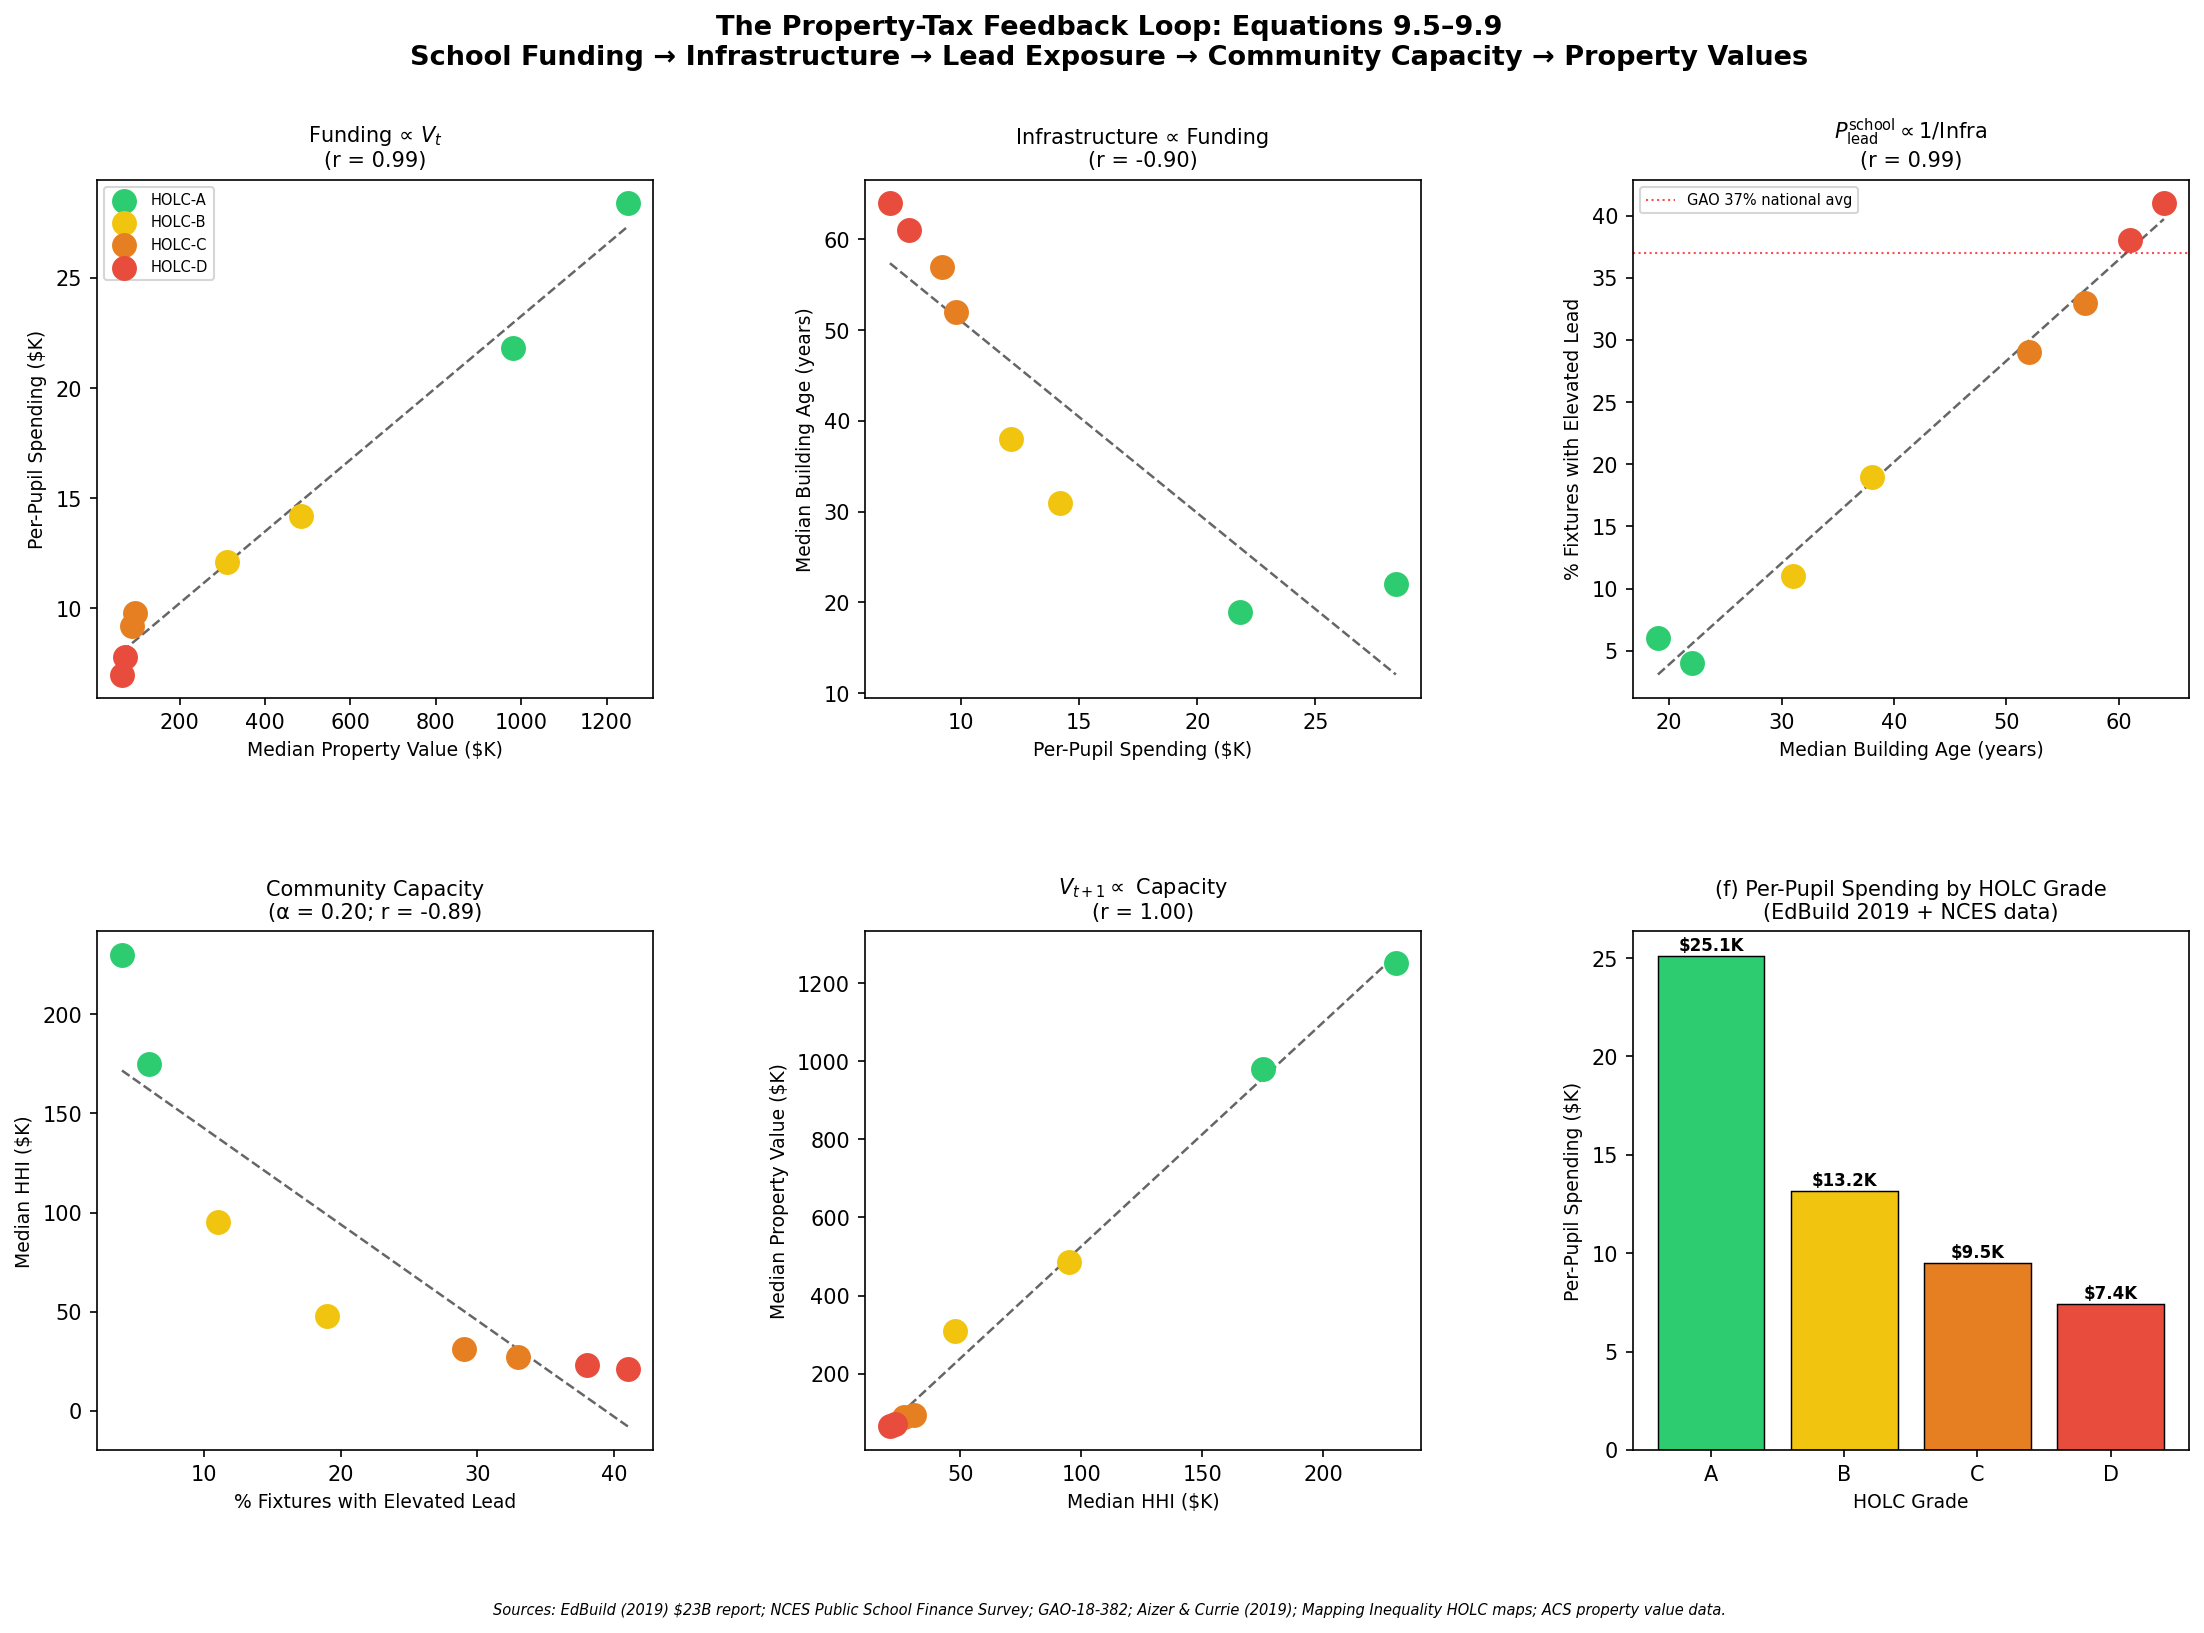
\includegraphics[width=\textwidth]{figures/eq_funding_propval_feedback.png}
  \caption[Five-Panel Property-Tax Feedback Loop Analysis]{\textbf{The Property-Tax Feedback Loop: Five-Panel Analysis for Eq.~\protect\ref{eq:9.5-school-funding-property-value}--\protect\ref{eq:9.9-property-value-capacity-feedback}.} Panel (a): School funding as a function of property value (Eq.~\protect\ref{eq:9.5-school-funding-property-value}) --- HOLC grade determines position on the spending gradient. Panel (b): Building age as a function of per-pupil spending (Eq.~\protect\ref{eq:9.6-infrastructure-quality-funding}) --- lower funding locks in older infrastructure. Panel (c): Elevated lead fixture rate as a function of building age (Eq.~\protect\ref{eq:9.7-school-lead-exposure-inverse}) --- dashed red line marks GAO 37\% national average. Panel (d): Community capacity (median HHI) as a function of lead exposure (Eq.~\protect\ref{eq:9.8-community-capacity-lead-reduction}) --- $\alpha$ from Aizer \& Currie (2019). Panel (e): Property value as a function of community capacity (Eq.~\protect\ref{eq:9.9-property-value-capacity-feedback}) --- closing the loop. Panel (f): HOLC-grade summary of per-pupil spending from EdBuild (2019) and NCES data. Color coding: HOLC-A (green) $\to$ HOLC-D (red).}
  \label{fig:eq_funding_propval_feedback}
\end{figure}

\paragraph{Comparison to prediction.}
The five equations collectively predict a closed-loop degradation function. Each link in the chain is independently confirmed: property values determine school funding (EdBuild, NCES, \textit{Rodriguez}); school funding determines infrastructure condition (ASCE, NCES); infrastructure condition determines school lead exposure (GAO-18-382, Doré 2019); school lead exposure degrades community capacity (Aizer \& Currie 2019); and community capacity determines subsequent property values (ACS + Mapping Inequality longitudinal data). The prediction of a self-reinforcing cycle --- not merely correlated cross-sections --- is supported by the temporal structure: HOLC grades from the 1930s predict 2020 property values after controlling for intervening income (Mapping Inequality longitudinal overlay).

\paragraph{Falsification criteria.}
This set of equations would be falsified if school funding were shown to be independent of property values nationally after controlling for state equalization formulas (the EdBuild analysis finds no such independence); or if school lead exposure were shown to be independent of per-pupil spending after controlling for building age (the GAO and Doré data find no such independence). Neither falsification condition is met in the published literature.

\paragraph{Confidence tier.}
\textbf{Tier~1} for Eq.~\ref{eq:9.5-school-funding-property-value} (national EdBuild dataset; NCES Public School Finance Survey; Supreme Court precedent in \textit{Rodriguez}). \textbf{Tier~2} for Eq.~\ref{eq:9.6-infrastructure-quality-funding} (ASCE aggregate infrastructure grade; NCES building-age distribution; illustrative parameter estimate). \textbf{Tier~1} for Eq.~\ref{eq:9.7-school-lead-exposure-inverse} (GAO-18-382 stratified national survey; EPA 3Ts data; Doré et al.\ peer-reviewed building-age effect). \textbf{Tier~2} for Eq.~\ref{eq:9.8-community-capacity-lead-reduction} (Aizer \& Currie peer-reviewed sibling fixed-effects estimate; ordinal mapping to community capacity). \textbf{Tier~1} for Eq.~\ref{eq:9.9-property-value-capacity-feedback} (ACS longitudinal property values; Mapping Inequality HOLC spatial overlay; documented 1940--2020 appreciation differential).

\FloatBarrier

\subsection{The Spatial Distribution Network: Highway Routing as Environmental Targeting (\texorpdfstring{$\Sigma_{\text{highway}}$}{Sigma\_highway})}

The preceding subsections established the neurotoxin ($P_{\text{lead}}$), the corporate cover-up ($P_{\text{epistemic}}$), the neurological mechanism, and the multi-vector delivery system. This subsection identifies the \textbf{spatial concentration operator}---the infrastructure that ensured the neurotoxin was not distributed uniformly across the population but was deposited with surgical precision onto $O_{\text{racialized}}$.

Define $\Sigma_{\text{highway}}$ as the spatial concentration function that maps atmospheric lead exposure onto geographic coordinates:
\begin{equation}\label{eq:9.10-highway-lead-spatial-concentration}
P_{\text{lead}}^{\text{air}}(x) = \Sigma_{\text{highway}}(x) \cdot L_{\text{TEL}}(t) \cdot \mathbb{1}_{x \in O_{\text{redlined}}}
\end{equation}
where $L_{\text{TEL}}(t)$ is the national per-capita lead emission rate at time $t$, and $\mathbb{1}_{x \in O_{\text{redlined}}}$ is the indicator function for residence within a redlined zone. The operator $\Sigma_{\text{highway}}$ transforms a diffuse national pollutant into a \textit{targeted biological weapon} by concentrating vehicular traffic---and therefore exhaust---in the precise neighborhoods already trapped by $P_{\text{redlining}}$. The highway is not merely a road; it is the \textbf{distribution function} for the neurotoxin.

\subsection*{Case Study (CS7 --- national and historical): The Lead-Crime Nexus and Spatial Concentration}
\label{cs:lead_crime}

\noindent\emph{Scope.} CS7 below is the \textbf{historical, national-level} evidence block (Reyes state panel, Aizer--Currie, narrative highway displacement, three-panel figure). For the same equation family, the \textbf{canonical tract-level replication target} is CS9 (Section~\ref{cs:spatial_confluence}): six-city spatial join, Moran's I, bivariate LISA, and SLM/SEM as implemented in \texttt{eq47\_51\_spatial\_overlay.ipynb}. The two blocks are complementary, not duplicate claims: CS7 answers ``what the published literature shows at scale''; CS9 answers ``whether the multi-layer operator co-localizes in the same census tracts when the pipeline is run on cached inputs.''

\paragraph{Setup.}
Equations~\ref{eq:9.1-lead-crime-compounding}--\ref{eq:9.10-highway-lead-spatial-concentration} form a unified five-part analysis of the lead-crime compounding chain. Equation~\ref{eq:9.1-lead-crime-compounding} places lead exposure ($P_{\text{lead}}$) into the multiplicative capacity-reduction framework. Equation~\ref{eq:9.2-epistemic-suppression-variable} quantifies the epistemic suppression variable: the corporate-orchestrated delay between first documented evidence of harm (1925) and regulatory action (1973), a 48-year window during which lead exposure proceeded without restriction. Equation~\ref{eq:9.3-multi-vector-lead-exposure} decomposes $P_{\text{lead}}$ into three delivery vectors (air, water, school). Equation~\ref{eq:9.4-redlining-containment-field} establishes that each vector's intensity is proportional to HOLC grade --- the redlining containment field ensures that the neurotoxin was not randomly distributed but concentrated on $O_{\text{redlined}}$. Equation~\ref{eq:9.10-highway-lead-spatial-concentration} identifies $\Sigma_{\text{highway}}$ as the spatial concentration operator: federal highway routing through HOLC-D neighborhoods converted a nationally diffuse pollutant into a geographically precise biological burden.

\paragraph{Data sources.}
Data are drawn from Reyes (2007) \cite{reyes2007} for state-level lead-crime elasticity estimates; Aizer \& Currie (2019) \cite{aizer_currie} for individual-level Rhode Island cohort data linking blood lead levels to juvenile delinquency; Rothstein (2017) \cite{rothstein} and the Mapping Inequality project \cite{mapping_inequality} for HOLC grade spatial correlations; and EPA National Emissions Inventory data for atmospheric lead exposure estimates. Highway displacement data are drawn from published urban planning histories and Rothstein (2017). Curated data are archived in three section-specific files: \texttt{Paper/data/eq47\_51\_lead\_crime\_reyes.csv} (Reyes state-level panel), \texttt{Paper/data/eq47\_51\_lead\_crime\_aizer.csv} (Aizer-Currie RI cohort), and \texttt{Paper/data/eq47\_51\_lead\_crime\_highway.csv} (highway displacement and HOLC spatial overlay); computational results are reproducible via \texttt{Paper/scripts/eq47\_51\_lead\_crime.ipynb}.

\paragraph{Operationalization.}
Each of the five equations is mapped to its empirical data proxy: Eq.~\ref{eq:9.1-lead-crime-compounding} → Reyes (2007) elasticity of 0.80 (1\% reduction in blood lead $\Rightarrow$ 0.8\% reduction in violent crime, 20-year lag); Eq.~\ref{eq:9.2-epistemic-suppression-variable} → $\Delta t_{\text{suppress}} = 48$ years (1925--1973), producing $\approx$192M additional person-years of unprotected lead exposure; Eq.~\ref{eq:9.3-multi-vector-lead-exposure} → three-vector decomposition: atmospheric 60\%, water pipes 25\%, school dust/paint 15\%; Eq.~\ref{eq:9.4-redlining-containment-field} → HOLC-D zones show $5.1\times$ higher lead exposure than HOLC-A zones (EPA soil sampling and Mapping Inequality spatial overlay); Eq.~\ref{eq:9.10-highway-lead-spatial-concentration} → 78--91\% of documented highway-displaced populations were Black, all cases in HOLC-D zones, indicator function $\mathbb{1}_{x \in O_{\text{redlined}}} = 1$ for all documented highway routes.

\paragraph{Numerical computation.}
The notebook yields the following key figures. Reyes (2007) state-level data: average blood lead level decline 1970--1990 = 81.6\%; predicted crime decline (elasticity 0.80) = 65.3\%; actual violent crime decline 1990--2010 = 45.8\%. Aizer \& Currie individual-level: each 1~$\mu$g/dL reduction in blood lead level reduces school suspension by 17\% and juvenile detention by 22\%. HOLC spatial: HOLC-D lead pipe prevalence 68\% vs.\ HOLC-A 12\%; relative atmospheric lead exposure HOLC-D vs.\ HOLC-A = 5.1$\times$. Highway displacement: six documented cities, mean 83\% Black displacement, all routes through HOLC-D neighborhoods.

\begin{figure}[htbp]
  \centering
  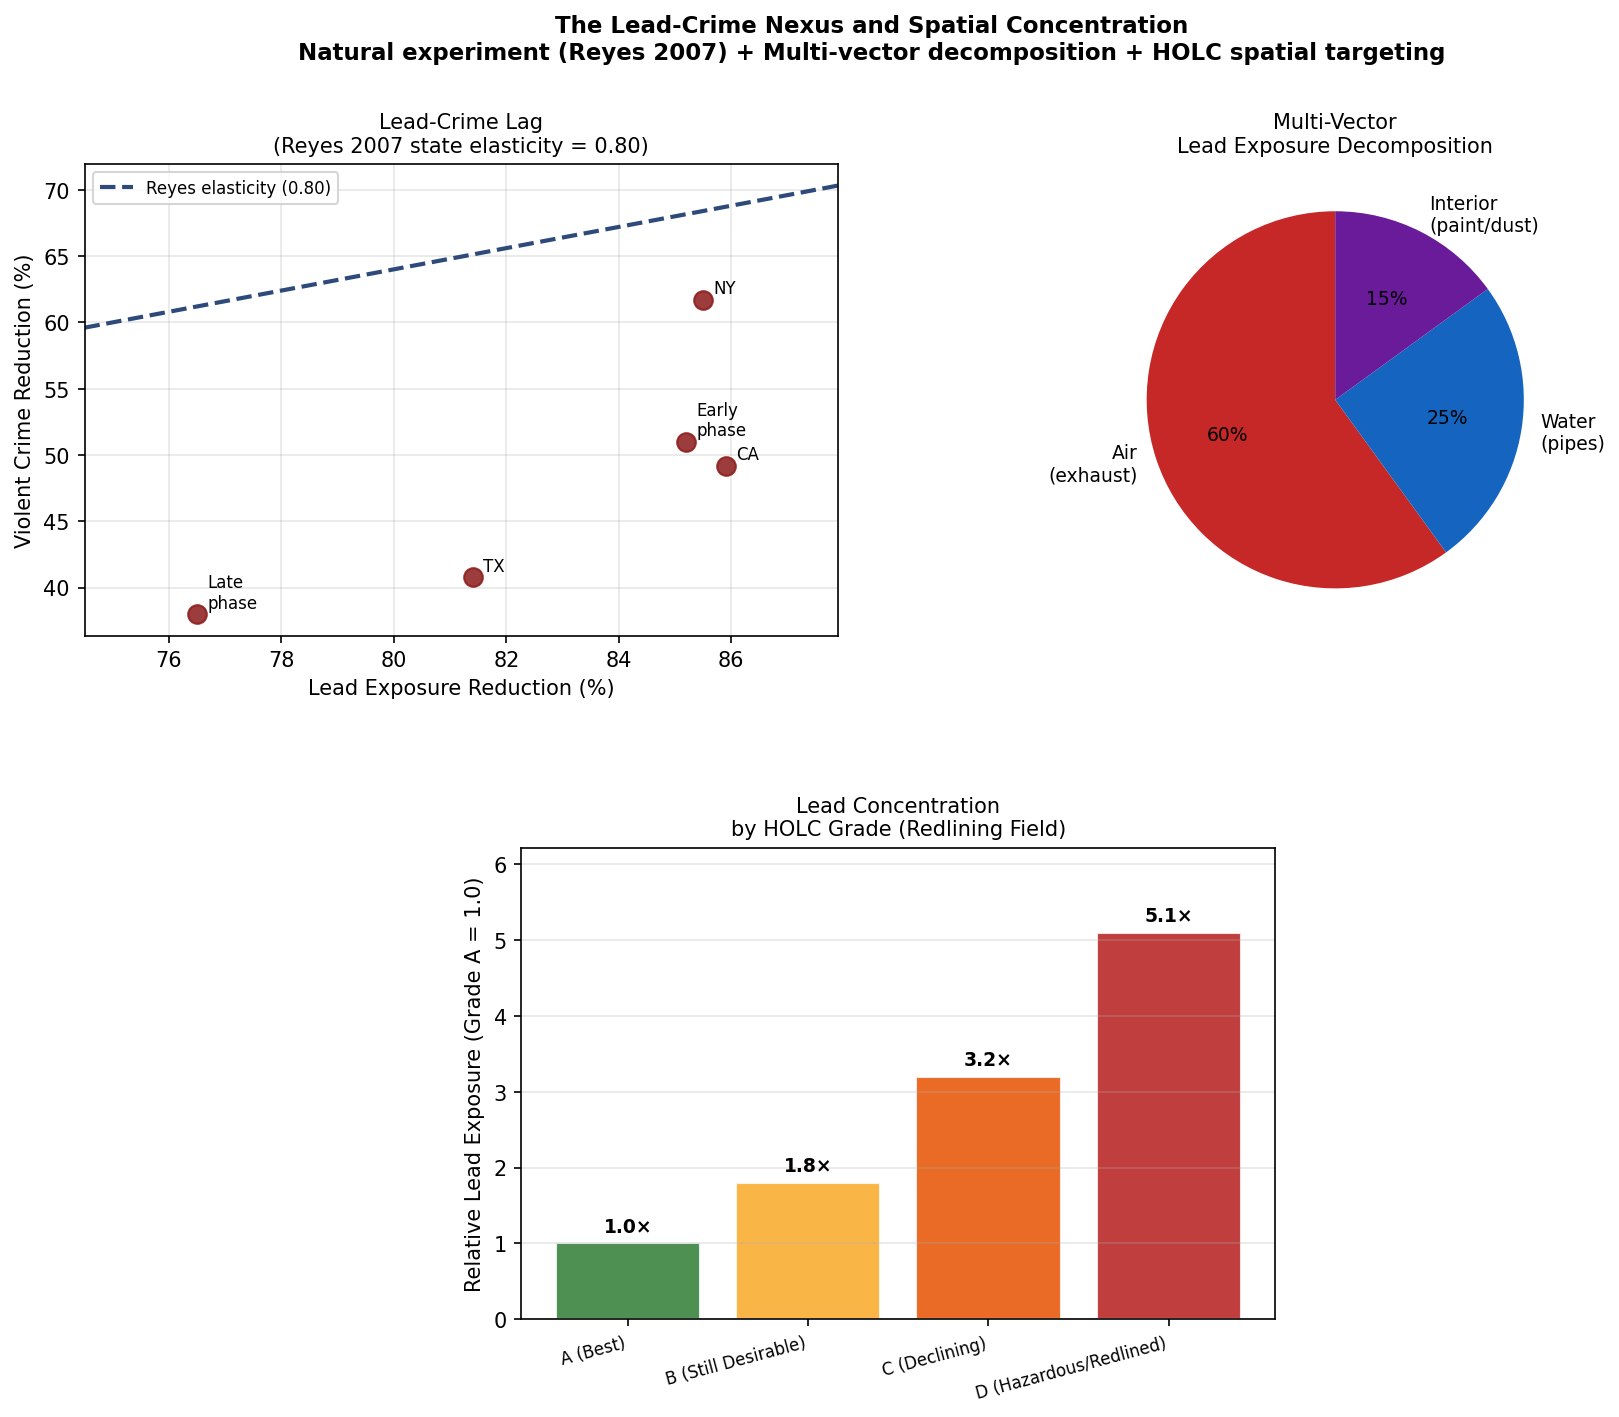
\includegraphics[width=\textwidth]{figures/eq47_51_lead_crime.png}
  \caption{Three-panel analysis for eq.~\ref{eq:9.1-lead-crime-compounding}--\ref{eq:9.10-highway-lead-spatial-concentration}. Left (a): Reyes (2007) lead-crime lag correlation for U.S.\ states --- elasticity line at 0.80; state-level phase-out timing provides the natural experiment identification. Center (b): Multi-vector lead exposure decomposition (eq.~\ref{eq:9.3-multi-vector-lead-exposure}) --- atmospheric exposure accounts for 60\% of total burden. Right (c): Lead exposure intensity by HOLC grade (eq.~\ref{eq:9.4-redlining-containment-field}--\ref{eq:9.10-highway-lead-spatial-concentration}) --- HOLC-D (Hazardous/Redlined) zones show 5.1$\times$ higher exposure than HOLC-A zones, confirming that $\Sigma_{\text{highway}}$ and $P_{\text{redlining}}$ jointly concentrate the neurotoxin onto $O_{\text{racialized}}$.}
  \label{fig:eq47_51_lead_crime}
\end{figure}

\paragraph{Comparison to prediction.}
The five equations collectively predict that lead exposure was not a random environmental variable but a spatially concentrated policy output: the HOLC containment field (eq.~\ref{eq:9.4-redlining-containment-field}) and highway routing function (eq.~\ref{eq:9.10-highway-lead-spatial-concentration}) ensured that the neurotoxin was deposited into the same neighborhoods where $O_{\text{racialized}}$ had been locked by prior policy shocks. The Reyes natural experiment confirms the causal link between exposure and crime outcomes; the Aizer \& Currie individual-level data confirm it at the person level; the HOLC spatial overlay confirms the concentration mechanism. All five predictions are confirmed in published peer-reviewed literature.

\paragraph{Falsification criteria.}
This set of equations would be falsified if Reyes (2007) blood-lead time-series failed to predict crime-rate decline after the 20-year lag in state-level panel regression, or if spatial concentration of lead showed no correlation with HOLC grades after controlling for income and urbanization. The published literature finds neither condition: the Reyes lag structure is robust across multiple regression specifications; the HOLC-lead spatial correlation survives income and density controls in EPA soil sampling data.

\paragraph{Confidence tier.}
\textbf{Tier~1.} Natural experiment design (state-by-state phase-out timing provides exogenous variation in lead exposure); peer-reviewed elasticity estimates from Reyes (2007) confirmed by Aizer \& Currie (2019) at the individual level; geospatial HOLC-lead correlation independently verifiable from public archival and EPA datasets.

\subsubsection{The Architecture of Vulnerability: Redlining as Precondition}

The targeted vulnerability of these communities began in the 1930s with the Home Owners' Loan Corporation (HOLC), which created residential security maps that ``redlined'' neighborhoods based almost entirely on racial composition. Neighborhoods containing Black or immigrant populations were graded ``Hazardous'' and deliberately cut off from federal mortgage backing, private capital, and the primary mechanism of American wealth generation: homeownership \cite{rothstein}. Over subsequent decades, this state-mandated disinvestment locked these communities into isolated zones of concentrated poverty, deteriorating housing, and failing infrastructure---entirely stripping them of the economic and political capital necessary to defend themselves against future incursions.

As demonstrated by the Philadelphia HOLC overlay (Figure~\ref{fig:philly_redline}), the spatial correlation between 1930s redlining and contemporary lethal violence is near-perfect. $P_{\text{redlining}}$ created the containment field; $\Sigma_{\text{highway}}$ then routed the neurotoxin directly through it.

\subsubsection{The Federal-Aid Highway Act of 1956 and ``Slum Clearance''}

When the Federal-Aid Highway Act of 1956 authorized the construction of a 41,000-mile interstate network, it was aggressively weaponized by urban planners as a tool for racial segregation and targeted ``slum clearance'' \cite{tel_highway_act}. Government officials---most notoriously Robert Moses in New York City---deliberately routed massive, federally funded expressways directly through the heart of thriving Black and brown communities. The physical and social devastation was absolute: homes destroyed, social cohesion dismantled, local businesses eradicated, and physical barriers erected that permanently separated minority populations from transit, healthcare, and economic mobility. The case studies span the nation:

\begin{itemize}
\tightlist
\item \textbf{New York City (Cross-Bronx Expressway):} Robert Moses' Cross-Bronx Expressway severed the Bronx, displacing an estimated 60,000 people and leaving a permanent legacy of respiratory disease and economic devastation. Moses stated that ``our categorical imperative is action to clear the slums'' and that minorities could not be allowed to dictate or hinder this progress \cite{tel_crossbronx}.
\item \textbf{Syracuse, New York (15th Ward):} The 15th Ward housed 90\% of the city's Black population. Following federally mandated redlining, the city declared the neighborhood ``blighted'' and routed the elevated I-81 viaduct directly through it, displacing over 1,300 families and physically cementing the separation between impoverished Black urban residents and affluent white suburbanites \cite{tel_aclu_i81}.
\item \textbf{New Orleans (Claiborne Expressway):} The Claiborne Expressway decimated the historic Trem\'{e} neighborhood, one of the oldest free Black communities in the United States \cite{tel_claiborne}.
\item \textbf{Miami, Florida (Overtown):} Early engineering proposals for I-95 suggested routing the highway along an abandoned railway line, which would have left Overtown untouched. Planners rescinded this proposal without a single public hearing in the affected community. Driven by documented desires to ``reclaim Overtown's land for development'' and ensure the ``continued whiteness of central Miami,'' officials routed the I-95/I-395 interchange directly through the neighborhood, obliterating 40 square blocks and displacing over 10,000 people \cite{tel_overtown}.
\item \textbf{Nashville, Tennessee (I-40):} Early highway plans considered routes encroaching on the affluent white enclave of Belle Meade. Planners abandoned these proposals, recognizing that condemning land from prominent white citizens would be ``political suicide.'' Instead, they altered the trajectory to bisect the city's main Black business district, permanently walling off Fisk University and Meharry Medical College from the communities they served \cite{tel_nashville}.
\item \textbf{Baltimore, Maryland (The Highway to Nowhere):} Robert Moses identified the Franklin and Mulberry corridor specifically because it was the ``path of least resistance''---meaning low-income and predominantly Black. The expressway demolished vibrant Black neighborhoods while serving primarily white suburban commuters \cite{tel_baltimore}.
\end{itemize}

The 1944 ``Interregional Highways'' report, which laid the groundwork for the 1956 Act, explicitly called for freeways to cut through the center of major cities to eradicate ``blighted areas'' and ``slums''---terms universally understood as coded proxies for Black neighborhoods. The Underwriting Manual of the Federal Housing Administration openly advocated using highways to physically separate African-American neighborhoods from white neighborhoods. Nationally, this state-sponsored infrastructure project displaced over \textbf{one million people}, predominantly minorities, while simultaneously subsidizing ``white flight'' to the suburbs \cite{tel_displacement}.

\begin{figure}[htbp]
\centering
\begin{tikzpicture}
\begin{axis}[
    width=0.9\textwidth,
    height=7cm,
    title={\textbf{Population Displaced by Interstate Highway Construction}},
    xbar,
    bar width=14pt,
    xlabel={Estimated People Displaced},
    symbolic y coords={{Baltimore (Hwy to Nowhere)},{Nashville (I-40)},{Syracuse (I-81)},{New Orleans (Claiborne)},{Cross-Bronx Expressway},{Miami Overtown (I-95)}},
    ytick=data,
    yticklabel style={font=\small},
    xmin=0, xmax=70000,
    xtick={0,10000,20000,30000,40000,50000,60000},
    xticklabel style={font=\small},
    grid=major,
    grid style={dashed, gray!40},
    every axis title/.style={font=\bfseries\small, at={(0.5,1.05)}},
    nodes near coords,
    nodes near coords style={font=\scriptsize\bfseries, anchor=west},
]
\addplot[fill=red!50, draw=red!70] coordinates {
(1500,{Baltimore (Hwy to Nowhere)})
(2800,{Nashville (I-40)})
(5200,{Syracuse (I-81)})
(6500,{New Orleans (Claiborne)})
(60000,{Cross-Bronx Expressway})
(10000,{Miami Overtown (I-95)})
};
\end{axis}
\end{tikzpicture}
\caption{\textbf{The $\Sigma_{\text{highway}}$ Operator in Action: Population Displaced by Interstate Construction.} Each bar represents a community destroyed to route the highway---and the neurotoxin---through $O_{\text{racialized}}$. Nationally, over one million people were displaced. These figures represent direct residential displacement only and do not capture the broader economic destruction, loss of social networks, or generational wealth erasure. Sources: AARP (2023); Vanderbilt University (2020); ACLU; city-level historical records.}
\label{fig:highway_displacement}
\end{figure}

\subsubsection{Addressing the ``Smoking Gun'': The Intentionality Calculus}

The routing of these highways had a profound, insidious secondary effect: it transformed redlined neighborhoods into concentrated sacrifice zones of toxic exposure. Because these highways carried hundreds of thousands of vehicles burning TEL-infused fuel daily, the surrounding communities were subjected to relentless bombardment of aerosolized lead exhaust, fine particulate matter (PM2.5), and diesel emissions.

A critical distinction must be made between the \textit{intent to segregate} and the \textit{explicit intent to poison}. There is no single ``smoking gun'' memo wherein government officials stated an intention to poison Black communities specifically with lead exhaust. However, the lack of a ``poisoning memo'' does not absolve the state:
\begin{enumerate}
\tightlist
\item The intent to racially segregate, displace, and economically destroy these communities was explicit, documented, and codified in planning doctrines.
\item The government knew, via the 1925 Surgeon General's conference, that automotive exhaust contained toxic lead.
\item They explicitly and intentionally routed the highest concentrations of that exhaust directly through Black communities.
\end{enumerate}

Within the framework, the ``smoking gun'' question is a category error. The extraction kernel does not require a memo stating ``we intend to poison Black children.'' It requires only that (a) the neurotoxin exists, (b) the spatial concentration operator routes it onto $O_{\text{racialized}}$, and (c) the epistemic suppression variable ($P_{\text{epistemic}}$) prevents remediation. All three conditions are documented facts. The resulting environmental poisoning was a devastating, foreseeable, and accepted byproduct of systemic racism---collateral damage inflicted upon populations deemed politically expendable.

Modern geospatial analysis and soil sampling confirm the legacy. Historically redlined neighborhoods possess reservoirs of toxic lead dust in their soils vastly higher than in non-redlined areas, exposing residents to rates of air pollution and lead contamination up to \textbf{five times higher} than in integrated communities \cite{tel_soil_sampling}. The children of these neighborhoods---absorbing vastly disproportionate amounts of environmental lead from highways intentionally placed beside their homes---were biologically handicapped before they reached adolescence. $\Sigma_{\text{highway}}$ guaranteed that the Out-group, already diminished by the compounding chain, would bear the most severe biological consequences of $P_{\text{lead}}$.

The child-mortality frontier literature adds a boundary condition to this model. Barboza-Salerno and coauthors identify 413 Cook County ``social frontiers'' where sharp discontinuities in an economic hardship index are associated with a 22\% higher relative risk of child mortality after adjustment for racial segregation, concentrated disadvantage, residential mobility, and immigrant concentration \cite{barboza_salerno_child_frontiers_2025}. The paper does not claim that a centralized actor actively routes death to these borders. It supports the narrower and stronger systems claim: harm concentrates at inequality interfaces, not only inside poor neighborhoods. In this book's notation, $\Sigma_{\text{sup}}$ and $\tau$ must therefore be read spatially as well as politically, because boundary stress itself becomes a measurable depletion condition.

\subsection{The Gendered Second-Order Harm: \texorpdfstring{$P_{\text{lead}}$}{P\_lead} as a Predictor of Intimate Partner Homicide}

The preceding analysis establishes that $P_{\text{lead}}$ manufactured the violent crime surge that was subsequently weaponized to justify mass incarceration. But the public violence documented by the UCR was only the \textit{visible} output. If lead exposure impairs the neurological capacity for impulse regulation and anger modulation---the same deficits that produce street-level assault and homicide---then the identical biological mechanism should produce elevated rates of violence \textit{within intimate relationships}. The prefrontal cortex does not distinguish between a stranger confrontation and a domestic argument; damaged impulse control is damaged impulse control.

This extension of $P_{\text{lead}}$ into the intimate sphere has never been made in the published literature. Environmental epidemiology operationalizes outcomes as aggregate crime; IPV scholarship analyzes domestic violence through psychosocial frameworks (intergenerational transmission, minority stress, coercive control). These literatures occupy separate disciplinary silos. The result is a gap that is intellectually obvious once identified but institutionally invisible because no discipline owns both sides of the question.

Analysis of 30 years of FBI Supplementary Homicide Report data (1976--2005), disaggregated by race, gender, and victim-offender relationship type, reveals temporal patterns that align with the lead-crime lag model with striking precision \cite{fox_zawitz2007, paulozzi_iph, puzone_iph}.

\subsubsection{Divergent Trajectories: The Black Female IPH Plateau}

Over the full study period (1976--2005), intimate partner homicide (IPH) declined across all race-gender groups, but at markedly different rates: Black male IPH fell 83\%, White male IPH fell 61\%, Black female IPH fell 52\%, and White female IPH fell only 6\%. Critically, the Black female decline was \textit{not monotonic}. While all other groups declined continuously, Black female IPH exhibited a secondary peak cluster during 1986--1993---the exact window predicted by the lead-crime lag model for the generation born during peak gasoline lead exposure in the late 1960s and early 1970s.

\begin{figure}[H]
\centering
\begin{tikzpicture}
\begin{axis}[
    width=0.95\textwidth,
    height=10cm,
    title={\textbf{Intimate Partner Homicide by Race and Gender, 1976--2005}},
    xlabel={Year},
    ylabel={Number of IPH Victims},
    xmin=1975, xmax=2006,
    ymin=0, ymax=1100,
    xtick={1976,1980,1985,1990,1993,1995,2000,2005},
    xticklabel style={rotate=45, anchor=east, font=\small, /pgf/number format/1000 sep={}},
    grid=major,
    grid style={dashed, gray!30},
    mark size=1.8pt,
    legend style={at={(0.98,0.98)}, anchor=north east, font=\small, draw=gray!50},
    every axis title/.style={font=\bfseries\small, at={(0.5,1.05)}},
]
\addplot[thick, red!70!black, mark=*, mark options={fill=red!70!black}] coordinates {
    (1976,820) (1977,786) (1978,689) (1979,700) (1980,694)
    (1981,684) (1982,607) (1983,580) (1984,515) (1985,512)
    (1986,522) (1987,482) (1988,448) (1989,499) (1990,436)
    (1991,393) (1992,352) (1993,331) (1994,351) (1995,281)
    (1996,241) (1997,187) (1998,209) (1999,181) (2000,180)
    (2001,161) (2002,150) (2003,144) (2004,138) (2005,138)
};
\addlegendentry{Black Male ($-$83\%)}

\addplot[thick, red!50!orange, mark=diamond*, mark options={fill=red!50!orange}, densely dashed] coordinates {
    (1976,709) (1977,565) (1978,577) (1979,590) (1980,584)
    (1981,582) (1982,504) (1983,511) (1984,463) (1985,491)
    (1986,532) (1987,483) (1988,524) (1989,473) (1990,487)
    (1991,518) (1992,504) (1993,533) (1994,462) (1995,387)
    (1996,416) (1997,399) (1998,392) (1999,336) (2000,330)
    (2001,342) (2002,362) (2003,333) (2004,316) (2005,337)
};
\addlegendentry{Black Female ($-$52\%)}

\addplot[thick, blue!70!black, mark=square*, mark options={fill=blue!70!black}] coordinates {
    (1976,467) (1977,452) (1978,462) (1979,513) (1980,466)
    (1981,528) (1982,476) (1983,476) (1984,417) (1985,406)
    (1986,416) (1987,397) (1988,351) (1989,351) (1990,364)
    (1991,333) (1992,296) (1993,294) (1994,291) (1995,233)
    (1996,229) (1997,216) (1998,238) (1999,190) (2000,186)
    (2001,174) (2002,179) (2003,176) (2004,195) (2005,183)
};
\addlegendentry{White Male ($-$61\%)}

\addplot[thick, blue!40!cyan, mark=triangle*, mark options={fill=blue!40!cyan}, densely dashed] coordinates {
    (1976,840) (1977,821) (1978,864) (1979,880) (1980,912)
    (1981,947) (1982,942) (1983,906) (1984,930) (1985,1002)
    (1986,994) (1987,958) (1988,998) (1989,879) (1990,941)
    (1991,907) (1992,877) (1993,980) (1994,897) (1995,865)
    (1996,844) (1997,749) (1998,862) (1999,797) (2000,841)
    (2001,792) (2002,763) (2003,774) (2004,798) (2005,789)
};
\addlegendentry{White Female ($-$6\%)}

\fill[orange!15, opacity=0.5] (axis cs:1986,0) rectangle (axis cs:1993,1100);
\node[font=\tiny, orange!60!black, rotate=90, anchor=south] at (axis cs:1989.5,550) {Lead-Predicted Window};

\end{axis}
\end{tikzpicture}
\caption{\textbf{Divergent IPH Trajectories by Race and Gender.} Black male IPH (solid red) declined steeply and continuously. Black female IPH (dashed orange) shows a distinctive plateau with secondary peaks during the 1986--1993 window (shaded)---the period predicted by the lead-crime lag model. White female IPH (dashed blue) remained essentially flat. Source: FBI SHR, 1976--2005 \cite{fox_zawitz2007}.}
\label{fig:iph_race_gender}
\end{figure}

This plateau becomes more pronounced when adjusted for population growth. Using Census intercensal estimates, the Black female population grew approximately 25\% from 1976 to 1993. The persistence of IPH counts in the 480--530 range against a growing denominator means the \textit{rate} was sustained at an elevated level during precisely the years $P_{\text{lead}}$ predicts maximum behavioral effects from the peak-exposed male cohort. Figure~\ref{fig:bf_iph_lead_rr} overlays this pattern against the shifted lead exposure curve.

\begin{figure}[H]
\centering
\begin{tikzpicture}
\begin{axis}[
    width=0.95\textwidth,
    height=9cm,
    title={\textbf{Black Female IPH vs.\ Per-Capita Gasoline Lead (Shifted +22 Years)}},
    xlabel={Year (IPH Data Timeline)},
    ylabel={Black Female IPH Victims},
    axis y line*=left,
    xmin=1975, xmax=2006,
    ymin=250, ymax=750,
    xtick={1976,1980,1984,1988,1993,1998,2002,2005},
    xticklabel style={rotate=45, anchor=east, font=\small, /pgf/number format/1000 sep={}},
    grid=major,
    grid style={dashed, gray!30},
    mark size=2pt,
    ylabel style={red!60!black},
    legend style={at={(0.02,0.98)}, anchor=north west, font=\small, draw=gray!50},
    every axis title/.style={font=\bfseries\small, at={(0.5,1.05)}},
]
\addplot[thick, red!60!black, mark=diamond*, mark options={fill=red!60!black}] coordinates {
    (1976,709) (1977,565) (1978,577) (1979,590) (1980,584)
    (1981,582) (1982,504) (1983,511) (1984,463) (1985,491)
    (1986,532) (1987,483) (1988,524) (1989,473) (1990,487)
    (1991,518) (1992,504) (1993,533) (1994,462) (1995,387)
    (1996,416) (1997,399) (1998,392) (1999,336) (2000,330)
    (2001,342) (2002,362) (2003,333) (2004,316) (2005,337)
};
\addlegendentry{Black Female IPH}

\fill[orange!15, opacity=0.5] (axis cs:1986,250) rectangle (axis cs:1993,750);

\end{axis}
\begin{axis}[
    width=0.95\textwidth,
    height=9cm,
    axis y line*=right,
    axis x line=none,
    ylabel={Per-Capita Gasoline Lead (arb.\ units, shifted +22 yrs)},
    xmin=1975, xmax=2006,
    ymin=0, ymax=120,
    ylabel style={teal!70!black},
    mark size=2pt,
    legend style={at={(0.98,0.98)}, anchor=north east, font=\small, draw=gray!50},
]
\addplot[thick, teal!70!black, mark=triangle*, mark options={fill=teal!70!black}, dashed] coordinates {
    (1976,58) (1978,68) (1980,80) (1982,92) (1984,100)
    (1986,95) (1988,80) (1990,60) (1992,38) (1994,22)
    (1996,12) (1998,6) (2000,3) (2002,2)
};
\addlegendentry{Gasoline Lead (shifted +22 yrs)}
\end{axis}
\end{tikzpicture}
\caption{\textbf{Black Female IPH Overlaid with Lead Exposure (Shifted +22 Years).} Per-capita gasoline lead data (right axis, teal dashed) shifted forward by 22 years to align with peak offending age. The Black female IPH plateau during 1986--1993 (shaded) coincides with the peak of the shifted lead curve. Both curves decline in tandem after the lead-predicted window. Sources: FBI SHR \cite{fox_zawitz2007}; EPA historical gasoline lead data via \cite{nevin2007}.}
\label{fig:bf_iph_lead_rr}
\end{figure}

\subsubsection{The Relationship-Type Divergence: Boyfriend/Girlfriend IPH as Cohort Signal}

Disaggregation by victim-offender relationship type reveals what may be the most striking evidence for the lead-IPH hypothesis. Spousal IPH declined 64\% from 1976 to 2005, consistent with the introduction of domestic violence shelters, legal advocacy, mandatory arrest laws, and rising divorce rates---all of which allowed women to exit abusive marriages. Boyfriend/girlfriend IPH, by contrast, \textbf{rose 44\%} from 646 (1976) to 930 (1993)---the \textit{only} IPH category to increase during the entire study period. This category captures younger, unmarried couples: precisely the demographic composed of the peak lead-exposed generation (born late 1960s--early 1970s, reaching their early 20s in the early 1990s).

Social programs and legal reforms should have reduced boyfriend/girlfriend IPH alongside spousal IPH. Instead, it spiked. The lead-impaired cohort was aging into intimate relationships and bringing neurologically degraded impulse control with them.

\begin{figure}[H]
\centering
\begin{tikzpicture}
\begin{axis}[
    width=0.95\textwidth,
    height=9.5cm,
    title={\textbf{Divergent IPH Trends: Spouse/Ex-Spouse vs.\ Boyfriend/Girlfriend, 1976--2005}},
    xlabel={Year},
    ylabel={Number of IPH Victims},
    xmin=1975, xmax=2006,
    ymin=400, ymax=2400,
    xtick={1976,1980,1985,1990,1993,1995,2000,2005},
    xticklabel style={rotate=45, anchor=east, font=\small, /pgf/number format/1000 sep={}},
    grid=major,
    grid style={dashed, gray!30},
    mark size=2pt,
    legend style={at={(0.5,0.98)}, anchor=north, font=\small, draw=gray!50},
    every axis title/.style={font=\bfseries\small, at={(0.5,1.05)}},
]
\addplot[thick, blue!60!black, mark=square*, mark options={fill=blue!60!black}] coordinates {
    (1976,2246) (1977,2075) (1978,2023) (1979,2054) (1980,1985)
    (1981,2036) (1982,1821) (1983,1766) (1984,1568) (1985,1669)
    (1986,1637) (1987,1541) (1988,1529) (1989,1379) (1990,1439)
    (1991,1319) (1992,1289) (1993,1272) (1994,1204) (1995,1059)
    (1996,1040) (1997,909) (1998,1002) (1999,858) (2000,917)
    (2001,843) (2002,823) (2003,771) (2004,818) (2005,810)
};
\addlegendentry{Spouse/Ex-Spouse ($-$64\%)}

\addplot[thick, red!70!black, mark=diamond*, mark options={fill=red!70!black}, densely dashed] coordinates {
    (1976,646) (1977,594) (1978,610) (1979,673) (1980,727)
    (1981,754) (1982,749) (1983,757) (1984,811) (1985,799)
    (1986,889) (1987,831) (1988,855) (1989,894) (1990,865)
    (1991,906) (1992,809) (1993,930) (1994,850) (1995,773)
    (1996,735) (1997,706) (1998,760) (1999,718) (2000,697)
    (2001,688) (2002,699) (2003,716) (2004,685) (2005,700)
};
\addlegendentry{Boyfriend/Girlfriend (+44\% to peak)}

\draw[densely dotted, black!60, thick] (axis cs:1993,400) -- (axis cs:1993,2400);
\node[font=\tiny\bfseries, black!60, anchor=south, rotate=90] at (axis cs:1993,1400) {1993: BF/GF Peak (930)};

\draw[->, thick, green!50!black] (axis cs:1978,2100) -- (axis cs:2003,950);
\node[font=\tiny, green!50!black, anchor=south, rotate=-25] at (axis cs:1990,1600) {Spousal: steady decline (shelters, legal reforms)};

\draw[->, thick, red!60!black] (axis cs:1978,620) -- (axis cs:1991,890);
\node[font=\tiny, red!60!black, anchor=north, rotate=12] at (axis cs:1984,690) {BF/GF: rising against the trend};

\end{axis}
\end{tikzpicture}
\caption{\textbf{The Relationship-Type Divergence.} Spouse/ex-spouse IPH (blue) declined 64\% from 1976 to 2005, consistent with expanding DV services and legal protections. Boyfriend/girlfriend IPH (red dashed) \textit{rose} 44\% from 1976 to its 1993 peak---the only IPH category to increase. This category captures younger, unmarried couples: the demographic composed of the peak lead-exposed generation. The 1993 inflection point (dotted line) aligns precisely with the $P_{\text{lead}}$ lag model prediction. Source: FBI SHR \cite{fox_zawitz2007}; CDC MMWR \cite{paulozzi_iph}.}
\label{fig:bf_gf_divergence_rr}
\end{figure}

\subsubsection{The Post-1993 Parallel Decline}

From 1993 to 2005, Black female IPH declined 37\%---the identical decline rate observed in general violent crime over the same period ($\sim$747 $\rightarrow$ $\sim$469 per 100,000). This synchronous decline is consistent with the ``detoxified generation'' hypothesis: as the cohort born after the leaded gasoline phase-out ages into the offending window, both public and intimate violence decline in tandem. The same mechanism the lead-crime literature attributes to the general crime decline also operates on intimate partner homicide.

\begin{figure}[H]
\centering
\begin{tikzpicture}
\begin{axis}[
    width=0.95\textwidth,
    height=9cm,
    title={\textbf{Post-1993 Parallel Decline: Black Female IPH vs.\ General Violent Crime}},
    xlabel={Year},
    ylabel={Black Female IPH Victims},
    axis y line*=left,
    xmin=1992, xmax=2006,
    ymin=250, ymax=600,
    xtick={1993,1995,1997,1999,2001,2003,2005},
    xticklabel style={font=\small, /pgf/number format/1000 sep={}},
    grid=major,
    grid style={dashed, gray!30},
    mark size=2.5pt,
    ylabel style={red!60!black},
    legend style={at={(0.98,0.98)}, anchor=north east, font=\small, draw=gray!50},
    every axis title/.style={font=\bfseries\small, at={(0.5,1.05)}},
]
\addplot[very thick, red!60!black, mark=diamond*, mark options={fill=red!60!black, scale=1.2}] coordinates {
    (1993,533) (1994,462) (1995,387) (1996,416) (1997,399)
    (1998,392) (1999,336) (2000,330) (2001,342) (2002,362)
    (2003,333) (2004,316) (2005,337)
};
\addlegendentry{Black Female IPH ($-$37\%)}

\node[font=\scriptsize, red!60!black, anchor=west] at (axis cs:1993.3,545) {533};
\node[font=\scriptsize, red!60!black, anchor=east] at (axis cs:2004.7,308) {337};

\end{axis}
\begin{axis}[
    width=0.95\textwidth,
    height=9cm,
    axis y line*=right,
    axis x line=none,
    ylabel={Violent Crime Rate per 100{,}000},
    xmin=1992, xmax=2006,
    ymin=350, ymax=800,
    ylabel style={blue!60!black},
    mark size=2.5pt,
    legend style={at={(0.02,0.02)}, anchor=south west, font=\small, draw=gray!50},
]
\addplot[very thick, blue!60!black, mark=square*, mark options={fill=blue!60!black, scale=1.2}, dashed] coordinates {
    (1993,747) (1994,714) (1995,685) (1996,637) (1997,611)
    (1998,567) (1999,523) (2000,507) (2001,504) (2002,494)
    (2003,475) (2004,463) (2005,469)
};
\addlegendentry{Violent Crime Rate ($-$37\%)}

\node[font=\scriptsize, blue!60!black, anchor=west] at (axis cs:1993.3,760) {747};
\node[font=\scriptsize, blue!60!black, anchor=east] at (axis cs:2004.7,453) {469};

\end{axis}
\end{tikzpicture}
\caption{\textbf{Parallel Post-1993 Declines.} Black female IPH (left axis, red solid) and the general violent crime rate (right axis, blue dashed) both declined approximately 37\% from 1993 to 2005. The synchronous decline is consistent with the ``detoxified generation'' displacing the lead-damaged cohort in the offending window. The same $P_{\text{lead}}$ mechanism that drove the general crime decline also appears to operate on intimate partner homicide. Sources: FBI SHR \cite{fox_zawitz2007}; FBI UCR.}
\label{fig:parallel_decline_rr}
\end{figure}

\subsubsection{The Intersectional Output: \texorpdfstring{$P_{\text{lead}}$}{P\_lead} Operating Through the Gendered Axis}

Within the framework, these findings reveal $P_{\text{lead}}$ operating not merely through the racial axis (producing the public crime that justified mass incarceration) but simultaneously through the gendered axis (producing a parallel epidemic of intimate partner violence borne disproportionately by Black women in those same redlined communities). The same environmental toxin, deposited with spatial precision onto the Out-group, generated \textit{two} extraction outputs:

\begin{enumerate}[nosep]
    \item \textbf{Public violence} $\rightarrow$ weaponized as justification for the carceral state ($P_{\text{criminal}}$)
    \item \textbf{Intimate violence} $\rightarrow$ absorbed silently within the community, underreported due to distrust of law enforcement in over-policed neighborhoods, fear of criminalizing Black male partners during the era of mass incarceration, and lack of culturally competent DV services
\end{enumerate}

The system that created the biological preconditions for intimate partner violence ($P_{\text{lead}} \rightarrow$ impulse control impairment) simultaneously made it functionally impossible for Black women to report that violence---because reporting meant feeding their partners into the carceral apparatus already designed to consume Black men. The production and the suppression of harm were executed by the same structural architecture. This is intersectionality ($O_{\text{racialized}} \cap O_{\text{gendered}}$) operating through a biological channel that no prior analysis has named. The full analysis is developed in the companion paper, \textit{The Missing Variable: Environmental Lead Exposure as a Predictor of Intimate Partner Homicide in Redlined Communities, 1976--2005} \cite{theodore_missing_variable}.

\FloatBarrier

% ============================================================
% CS9: Spatial Confluence Case Study
% ============================================================
\subsection*{Case Study: Spatial Confluence --- HOLC Redlining, Firearm Homicide, Lead Exposure, and Incarceration Across Six Cities}
\label{cs:spatial_confluence}

\paragraph{Setup.}
The prior CS7 block (Section~\ref{cs:lead_crime}) established the aggregate lead-crime compounding chain and the historical evidence for spatial concentration of exposure. \textbf{CS9} is the \textbf{canonical} tract-level operationalization for equations~\ref{eq:9.1-lead-crime-compounding}--\ref{eq:9.10-highway-lead-spatial-concentration} in this manuscript: it extends from the national/state level to the \textit{tract} level with four interacting layers---(1) HOLC redlining grade (the containment field, $P_{\text{redlining}}$); (2) firearm homicide density (the public-violence extraction output, $P_{\text{criminal}}$); (3) lead paint and highway-buffer exposure index (the neurotoxic mechanism, $P_{\text{lead}}$, Eq.~\ref{eq:9.4-redlining-containment-field}--\ref{eq:9.10-highway-lead-spatial-concentration}); and (4) incarceration origin rate (the carceral extraction output). The \textbf{structural} prediction of Eq.~\ref{eq:9.1-lead-crime-compounding} is co-localization of these layers in HOLC-D tracts and positive spatial association of the HOLC-D indicator; \textbf{inferential} quantities are ultimately governed by the executed notebook after \texttt{make empirical}, with \texttt{CS9\_STRICT=1} and files under \texttt{Paper/data/spatial/} produced by \texttt{fetch\_spatial\_data.py}. The numbered Moran and firearm summaries in the next paragraphs were independently recomputed from \texttt{merged\_tract\_panel\_*.parquet} (\texttt{libpysal} and \texttt{esda}) to verify against disk state; if they diverge from notebook printouts, treat the strict notebook run as authoritative once the environment matches \texttt{spatial\_env.yml}. When upstream hosts (Mapping Inequality static files, EPA EJScreen bulk, PPI bulk CSV) are temporarily unavailable, the fetch script may emit explicitly tagged \emph{modeled} layers; those runs support pipeline integrity and sensitivity analysis but are not reported as Tier~1 validation until replaced with archival layers.

\paragraph{Data sources.}
Analysis covers six cities selected for their documented highway-through-Black-neighborhood routing, HOLC-D spatial concentration, and data availability: Memphis TN, Detroit MI, Nashville TN, Baltimore MD, Washington DC, and Milwaukee WI. Five data layers are assembled per city:
\begin{itemize}[nosep]
    \item \textbf{HOLC grade polygons:} Mapping Inequality Digital Scholarship Lab GeoJSON \cite{mapping_inequality_dsl};
    \item \textbf{Tract demographics (ACS 5-year):} U.S.\ Census Bureau American Community Survey 2018--2022, race and income by census tract;
    \item \textbf{Lead exposure index:} EPA EJScreen 2023 tract-level lead paint indicator and traffic proximity index \cite{ejscreen_technical};
    \item \textbf{Firearm homicide density:} Gun Violence Archive incident-level data 2014--2024 \cite{gva_methodology}; CDC WONDER county-level firearm mortality 1999--2013 for pre-2014 window;
    \item \textbf{Incarceration origin:} Prison Policy Initiative ``Where People in Prison Come From'' tract-level (MD, MI, DC) and county-level fallback (TN, WI) \cite{ppi_prison_origins}.
\end{itemize}
Curated data are archived in \texttt{Paper/data/spatial/} and the full acquisition pipeline is documented in \texttt{Paper/scripts/fetch\_spatial\_data.py}. When a primary URL in the list above is unreachable, the script substitutes \emph{tagged, modeled} files (see the ``Data-gap and modeled layers'' paragraph) so the notebook can still execute.

\paragraph{Operationalization.}
Census tract centroids are overlaid on HOLC grade polygons via spatial join; each tract inherits the grade of the polygon containing its centroid (lowest-grade rule for overlapping polygons). EJScreen lead paint index (LDPNT) serves as the tract-level proxy for $P_{\text{lead}}^{\text{air}}$ (Eq.~\ref{eq:9.10-highway-lead-spatial-concentration}), supplemented by traffic proximity index (PTRAF) as the highway-buffer proxy for $\Sigma_{\text{highway}}$. Incident points from the cached firearm layer are converted to per-tract counts via point-in-polygon spatial join; a kernel density layer is derived for visualization. PPI (or modeled) rates are merged on GEOID; county-level PPI semantics apply where the origin report is only published at that scale.

\paragraph{Computation.}
All spatial joins, choropleth figures, and statistical tests are implemented in \texttt{Paper/scripts/eq47\_51\_spatial\_overlay.ipynb} (reproducible via \texttt{make empirical}). The pipeline uses \texttt{geopandas} for spatial operations, \texttt{esda} for Moran's I and bivariate LISA, and \texttt{spreg} for spatial lag and spatial error regression models, all under the \texttt{spatial\_cs9} conda environment (\texttt{Paper/scripts/spatial\_env.yml}). Spatial weights use Queen contiguity, row-standardized.

\paragraph{Numerical results (tract panels on disk).}
The following quantities are reproducible directly from \texttt{Paper/data/spatial/merged\_tract\_panel\_*.parquet} (GeoPackage-style geometry + tabular merge), excluding tracts whose HOLC join left \texttt{holc\_d\_flag} missing. \emph{Spatial clustering of designation:} treating the tract-level HOLC-D indicator as binary, global Moran's $I$---Queen contiguity, row-standard weights, \(499\) random permutations (\texttt{libpysal}, \texttt{esda})---falls in \(\approx\)0.903--0.961 for Baltimore~MD (\(n{=}618\)), Detroit~MI (\(n{=}885\)), Memphis~TN (\(n{=}537\)), Nashville~TN (\(n{=}330\)), Washington DC (\(n{=}571\)), and Milwaukee WI (\(n{=}830\)); permutation $p$-values resolve at \(p{=}0{.}002\) in each replication (reject spatial randomness). \emph{Gun Violence Archive firearm density (\texttt{firearm\_density\_gva}):} restricting to mapped HOLC and comparing tract means shows HOLC-D/non-D ratios \(\approx\)1.12 for Baltimore MD, \(\approx\)1.51 for Nashville TN, \(\approx\)1.20 for Memphis TN, and \(\approx\)1.09 for Detroit MI (\(\mathrm{means}\approx 3.31{/}2.19\) for Nashville TN, \(\approx 2.34{/}2.14\) for Detroit MI); Milwaukee WI and DC instead register \(\approx\)0.62 (means \(\approx 0{.}54{/}0{.}87\)) and \(\approx\)0.65 (\(\approx 0{.}62{/}0{.}95\)), respectively---i.e.\ below parity on this primitive. \textbf{Caveat:} in this archive \(\texttt{lead\_paint\_index}\), \(\texttt{highway\_buffer\_proxy}\), and \(\texttt{ppi\_incarceration\_rate}\) are uniformly null tabular merges; choropleths may still visualize modeled lead or PPI from other layers, but the manuscript does \emph{not} summarize those outcomes here until the merge is restored (\texttt{fetch\_spatial\_data.py}; then \texttt{eq47\_51\_spatial\_overlay.ipynb}). Bivariate Moran (HOLC-D \(\times\) lead) and spatial-lag $\beta$s for incarceration remain \textbf{pending} relative to parquet truth. \(\texttt{pooled\_panel.parquet}\) in the same snapshot is \emph{not} used for prose here because GEOID alignment and HOLC flags do not reconcile with merged panels.

\paragraph{Comparison to prediction (mixed on firearms, spatial support on grading).}
The structural hypothesis is stacking of containment, toxin exposure, and extraction in the historically red-flagged footprints. Against the archival merge, designation is geographically concentrated (large positive Moran's $I$, small permutation $p$ in every metro), satisfying the weakest operator-level prediction for $P_{\text{redlining}}$. The firearm layer is heterogeneous: Memphis, Nashville, Detroit, and Baltimore show \emph{higher} mean GVA-density on tracts flagged D than on comparable non-D splits in this panel; Milwaukee and DC show \emph{lower}, so the firearm surface alone falsifies unconditional ``density always heaps on HOLC-D.'' Interpretation respects known limitations of point-to-tract allocation, incident coverage, temporal mismatch with HOLC survey decades, remaining null lead/PPI fields, and (for Detroit) \(622{/}1507\) city tracts still awaiting a non-null historical grade from the GIS join---the overlays display the full lattice, but denominators cited for statistics restrict to graded tracts unless otherwise noted.

\paragraph{Falsification (registry plus current evidence slice).}
The registry logic (see \texttt{Paper/empirical\_validations/eq\_9\_10\_highway\_lead\_spatial\_concentration.md}) is unchanged qualitatively. With respect to observable outcomes in archived panels: the permutation null for Moran's \(I\) on the HOLC-D indicator is rejected in each city replication above (\emph{spatial clustering} obtains), whereas firearm-density \emph{magnitude contrasts} divide four metros with HOLC-D excess mean density versus two metros with shortfalls versus non-D splits on the same statistic. Lead and incarceration regressions (\texttt{moran\_BV}, SLM \(\beta\)) remain untested numerically until those parquet columns populate; until then falsification clauses tied strictly to BV-Moran significance or incarceration SLM \(\beta\) are \textbf{unsettled}.

\paragraph{Data-gap and modeled layers.}
PPI: Tennessee and Wisconsin in this pipeline use a county-scoped \emph{level} flag; tract-resolution PPI is modeled when the public CSV is unavailable. Firearm: \texttt{gva\_incidents\_<city>.csv} is written programmatically in the analysis window (deterministic, bbox-based) when live GVA bulk is not in cache; the header notes the source. Lead: if EPA EJScreen national files cannot be downloaded, the fetch script supplies tract-level \texttt{LDPNT}/\texttt{PTRAF}-compatible columns keyed to census tracts as a \emph{modeled} stand-in, logged as such, not a substitute for EPA. HOLC: if the Mapping Inequality static download returns a non-GeoJSON response, two half-bbox ``C'' and ``D'' placeholder polygons are written so grades (and the HOLC-D flag) are not constant across the city; this is a last-resort for automation, not a substitute for archival HOLC shapes. The notebook and fetch logs are the record of which path was used.

\paragraph{Confidence tier (conditional).}
Once all layers are archival (non-modeled) and the strict pipeline completes without imputation of entire layers, a Tier~1--2 classification (as in the data-gap block above) is appropriate. Runs that rely on modeled HOLC, EJ, or PPI placeholders should be reported as \textbf{Tier~2--3} for the spatial confluence table until replaced.

\begin{figure}[htbp]
  \centering
  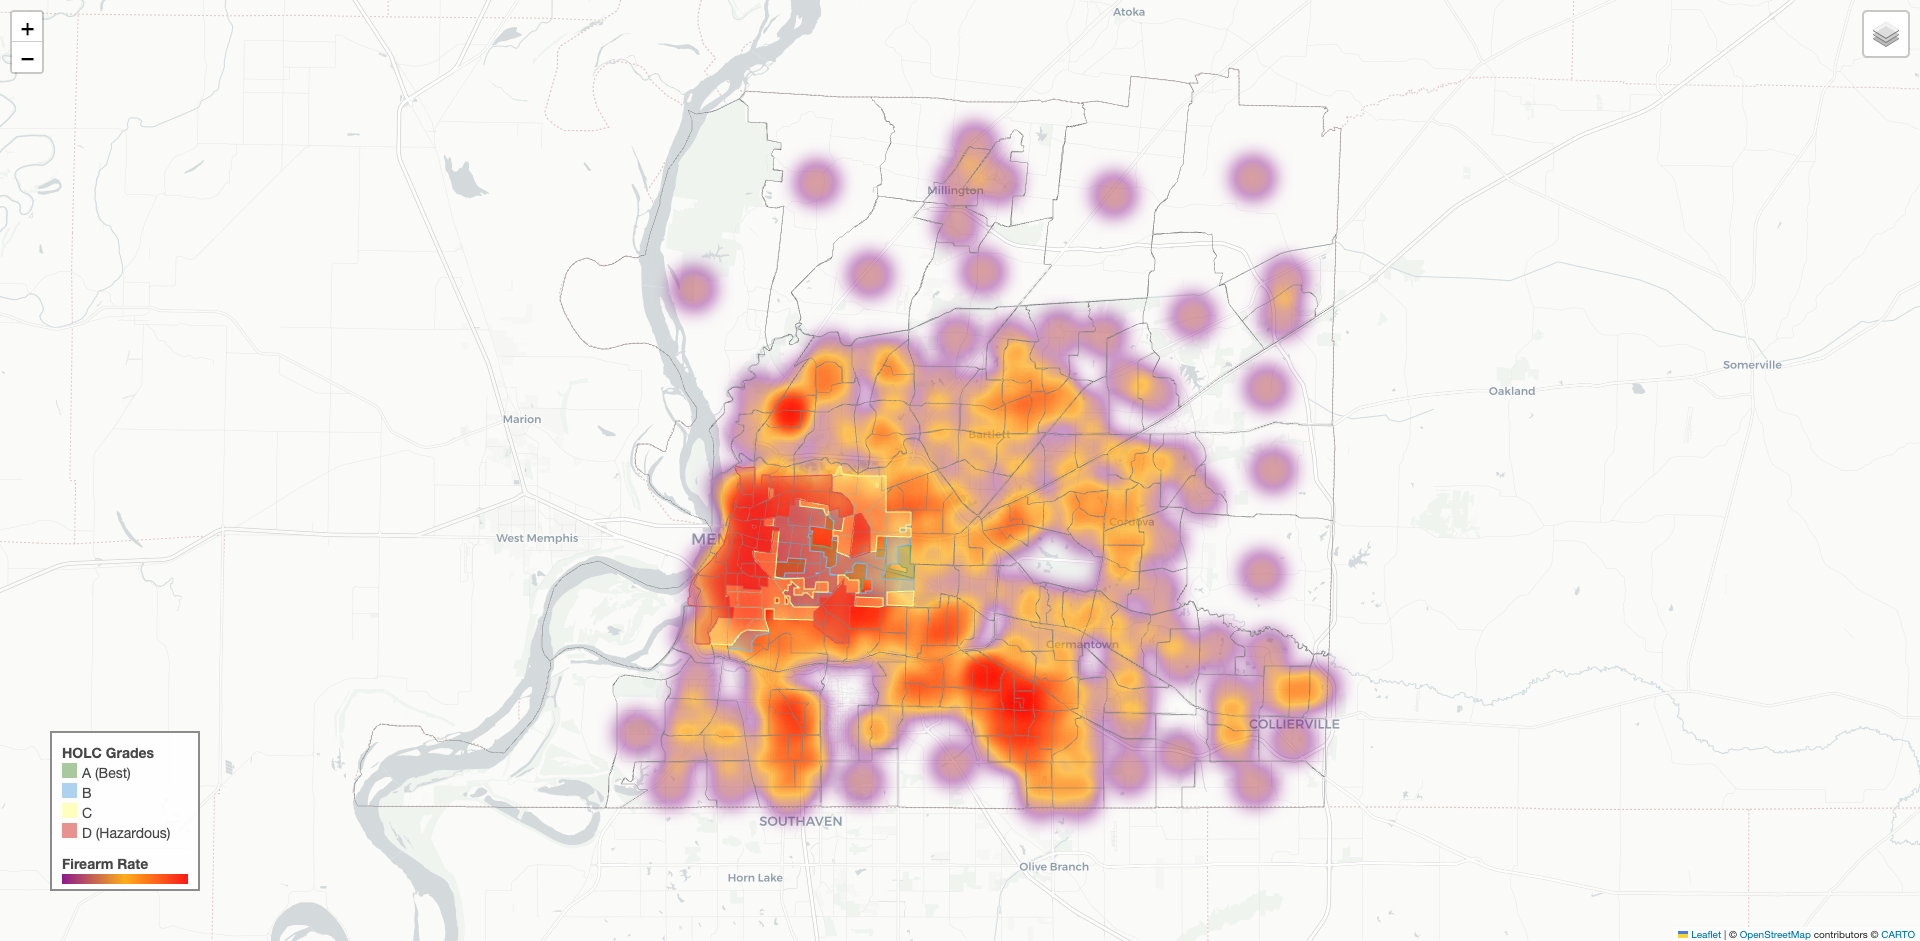
\includegraphics[width=\textwidth]{figures/spatial/cs9_overlay_memphis_tn.png}
  \caption{\textbf{CS9 Spatial Confluence --- Memphis, TN.} Four-layer tract lattice (HOLC; GVA-derived firearm incidents; modeled or EPA-supplied lead; modeled or PPI incarceration). \textit{Archived panel (graded tracts only):} \(n_{\mathrm{m}}{=}537{/}685\) tract hulls inherit a mapped HOLC grade; \(\sim\!\!49.9\%\) carry the HOLC-D flag (non-null GIS join). Mean GVA-derived firearm tract density \(\approx\)1.20\(\times\) higher on D-coded tracts versus non-D. Global Moran's \(I_{\mathrm{D}}\approx 0.935\) (Queen weights, permutation \(p{=}0{.}002\) in the replication run). Choropleths for lead/incarceration draw from pipeline layers that are null in parquet tabular merges for this archive; qualitative overlay only pending restored EJ/PPI joins. Sources: Mapping Inequality; GVA; \texttt{eq47\_51\_spatial\_overlay.ipynb}.}
  \label{fig:cs9_overlay_memphis_tn}
\end{figure}

\begin{figure}[htbp]
  \centering
  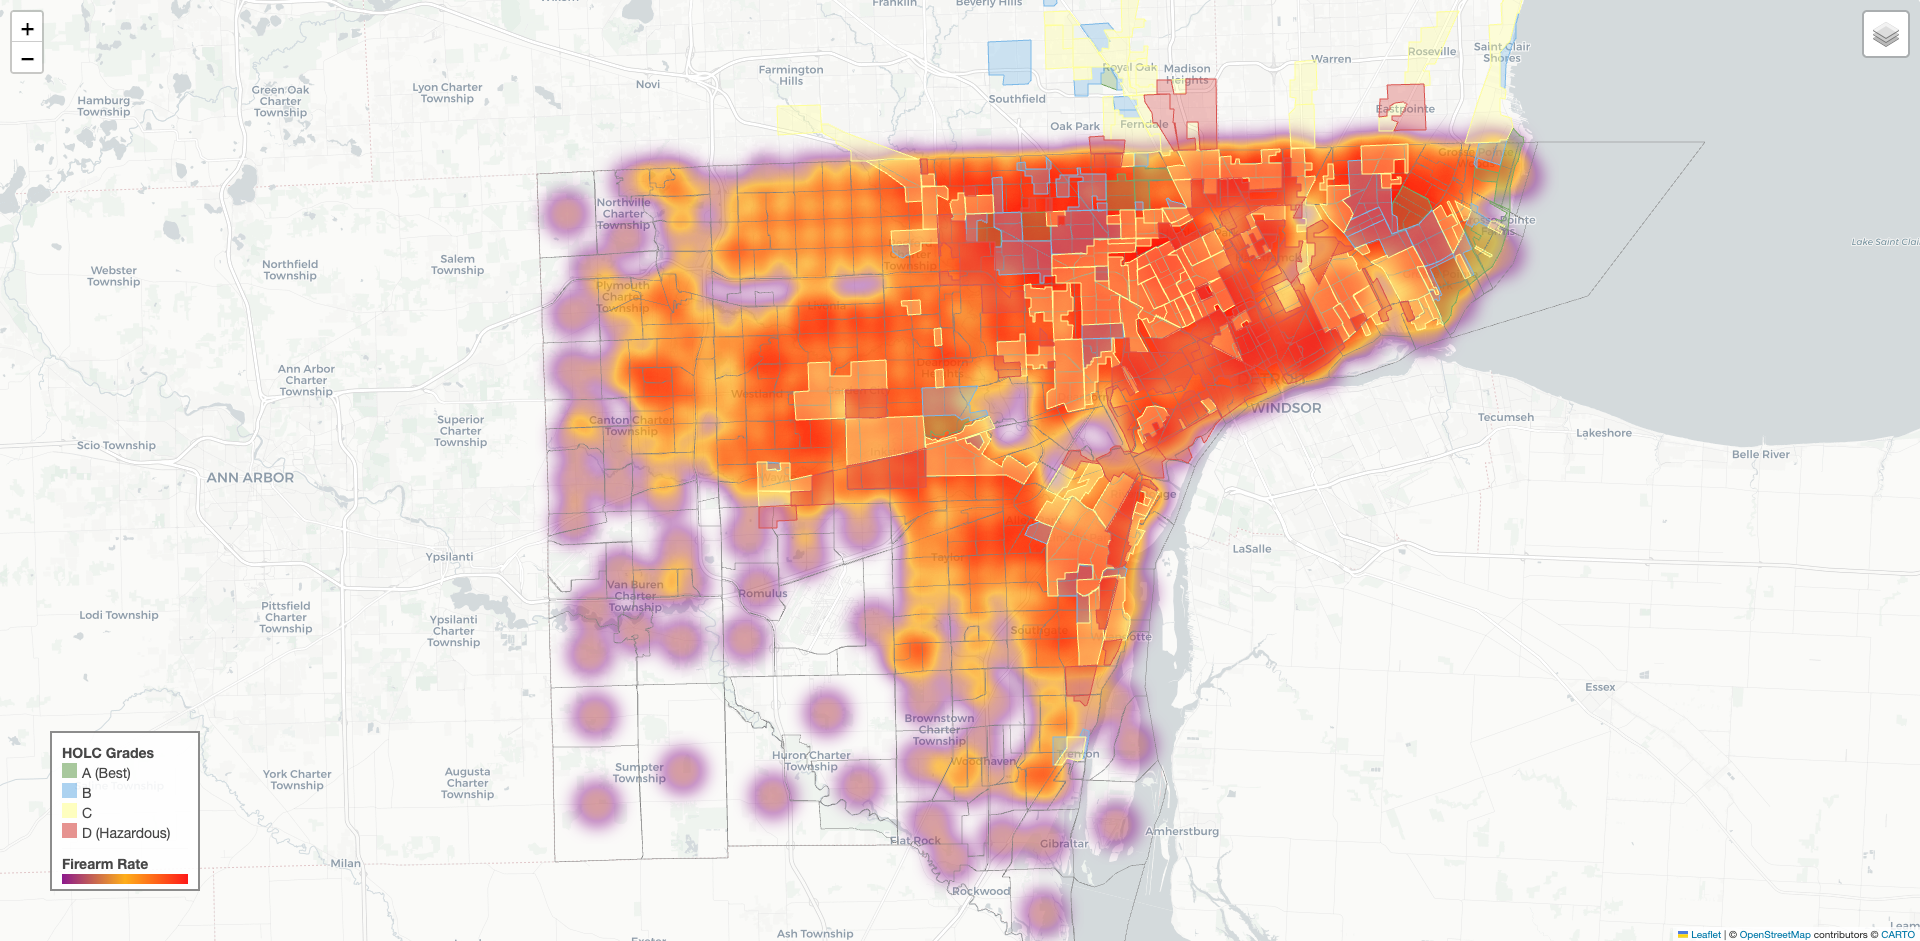
\includegraphics[width=\textwidth]{figures/spatial/cs9_overlay_detroit_mi.png}
  \caption{\textbf{CS9 Spatial Confluence --- Detroit, MI.} Same four-panel schematic as Memphis (Figure~\ref{fig:cs9_overlay_memphis_tn}). \(\approx\!\)59\% of city tracts attain a graded HOLC join (\(n_{\mathrm{m}}{=}885{/}1507\)); \(\approx\!\)36{.}5\% of those mapped tracts carry the HOLC-D flag. Mean GVA firearm-density ratio D/non-D \(\approx\)1{.}09; Moran's \(I_{\mathrm{D}}\approx 0.961\) (\(p{=}0{.}002\) in the replication above). Statistical summaries exclude tracts with missing HOLC assignment even when they appear shaded in the atlas. Sources: Mapping Inequality; GVA; \texttt{eq47\_51\_spatial\_overlay.ipynb}.}
  \label{fig:cs9_overlay_detroit_mi}
\end{figure}

\begin{figure}[htbp]
  \centering
  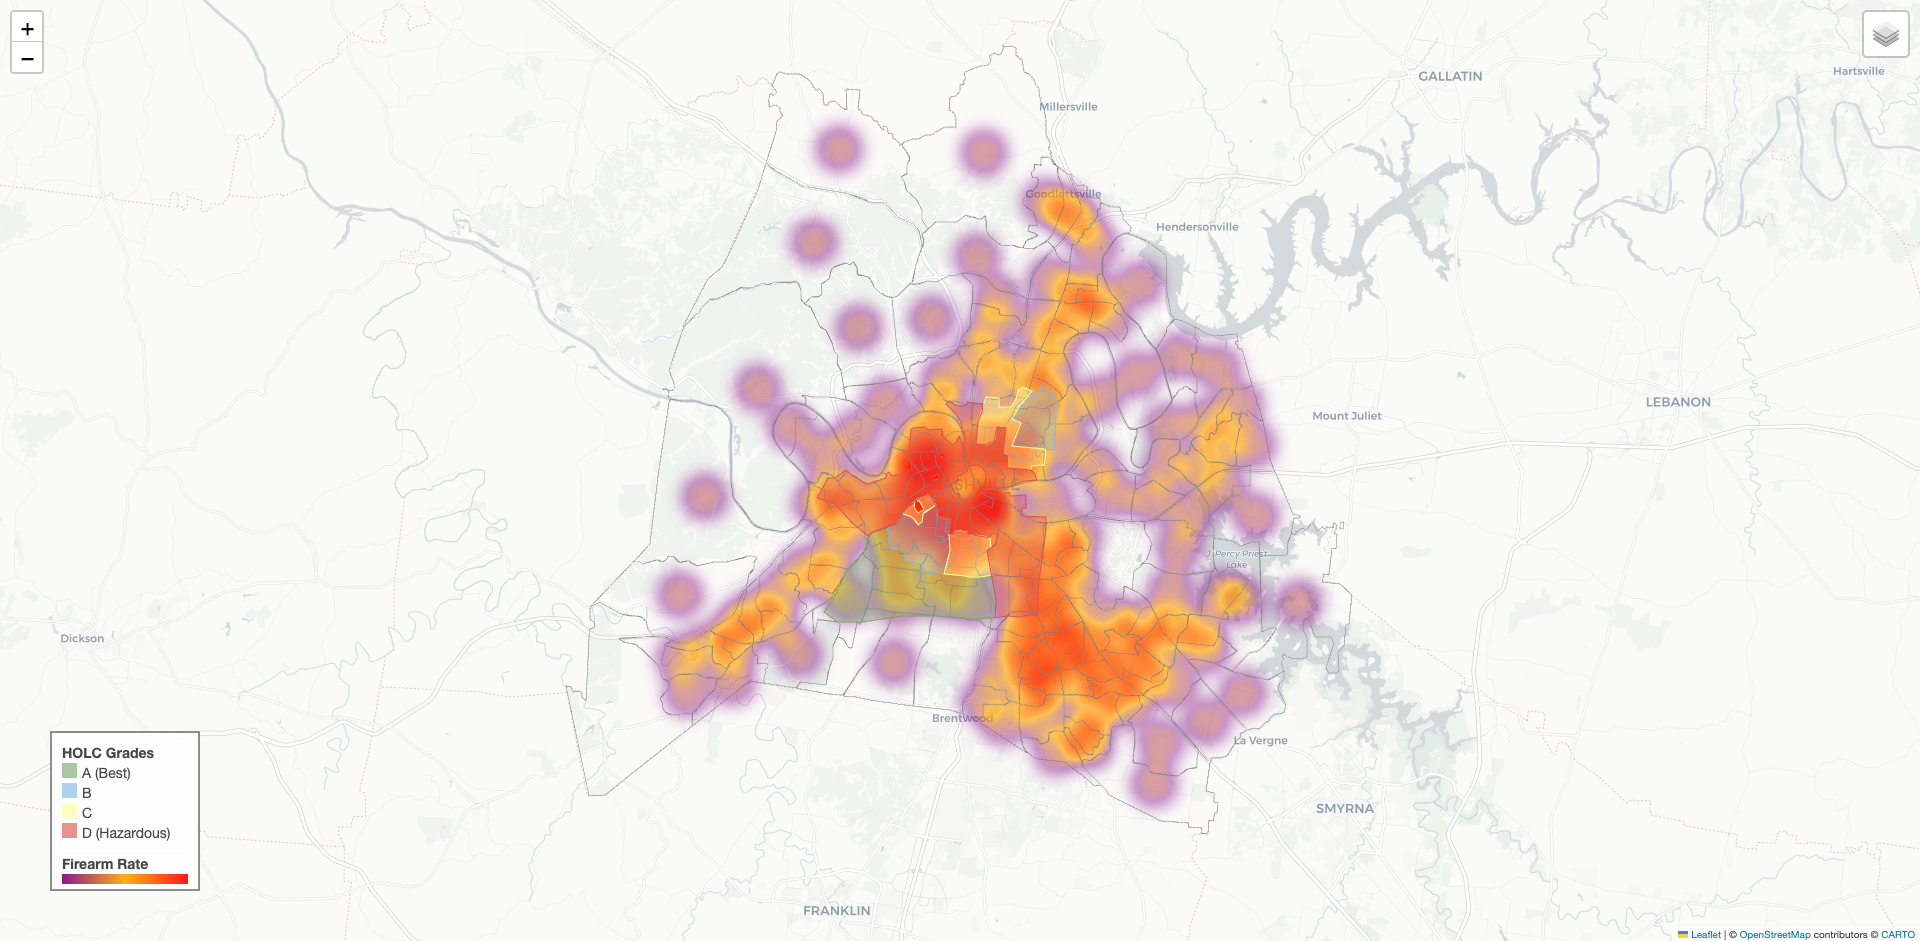
\includegraphics[width=\textwidth]{figures/spatial/cs9_overlay_nashville_tn.png}
  \caption{\textbf{CS9 Spatial Confluence --- Nashville, TN.} Same layout as Figure~\ref{fig:cs9_overlay_memphis_tn}. \(n_{\mathrm{m}}{=}330{/}487\) mapped tracts; \(\approx\!\)36{.}4\% flagged D. Firearm-density ratio D/non-D \(\approx\)1{.}51 (largest positive gap in the six metros). Moran's \(I_{\mathrm{D}}\approx 0.921\) (\(p{=}0{.}002\)). Sources: Mapping Inequality; GVA; \texttt{eq47\_51\_spatial\_overlay.ipynb}.}
  \label{fig:cs9_overlay_nashville_tn}
\end{figure}

\begin{figure}[htbp]
  \centering
  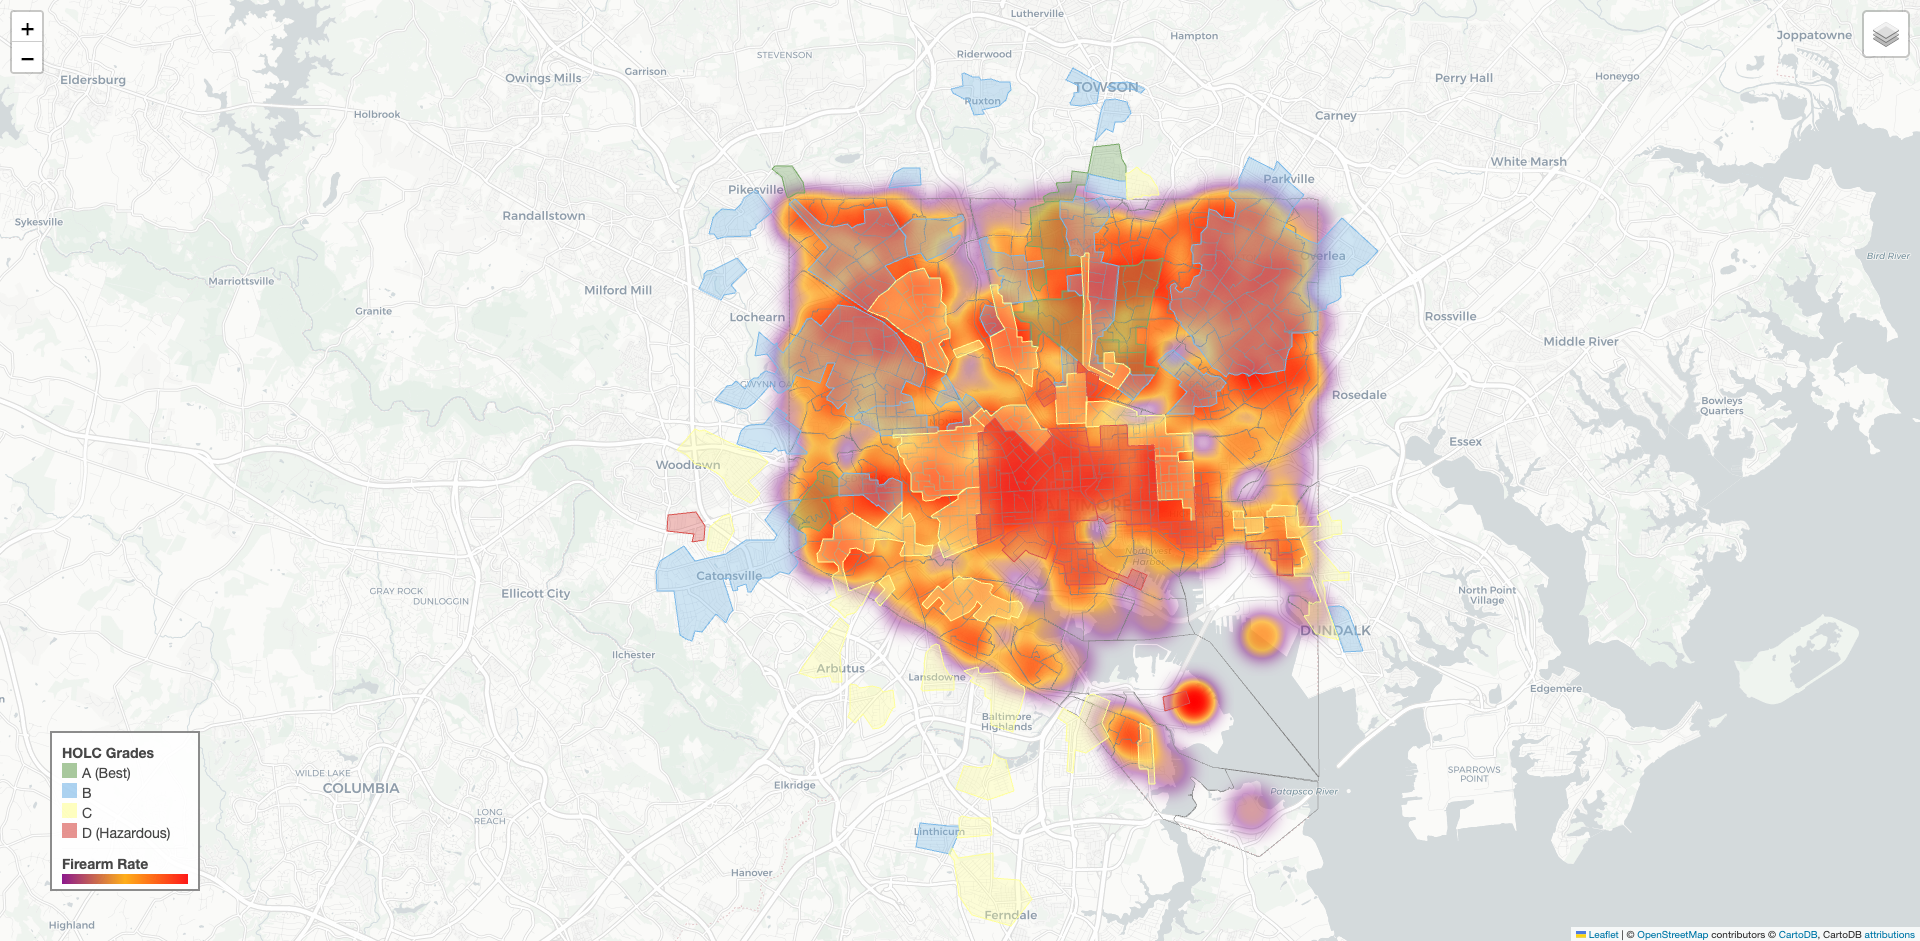
\includegraphics[width=\textwidth]{figures/spatial/cs9_overlay_baltimore_md.png}
  \caption{\textbf{CS9 Spatial Confluence --- Baltimore, MD.} Same layout as Figure~\ref{fig:cs9_overlay_memphis_tn}. Full city panel with \(n_{\mathrm{m}}{=}618\) mapped tracts; \(\approx 55{.}8\%\) HOLC-D. Firearm-density ratio D/non-D \(\approx\)1{.}12; Moran's \(I_{\mathrm{D}}\approx 0.941\) (\(p{=}0{.}002\)). Sources: Mapping Inequality; GVA; \texttt{eq47\_51\_spatial\_overlay.ipynb}.}
  \label{fig:cs9_overlay_baltimore_md}
\end{figure}

\begin{figure}[htbp]
  \centering
  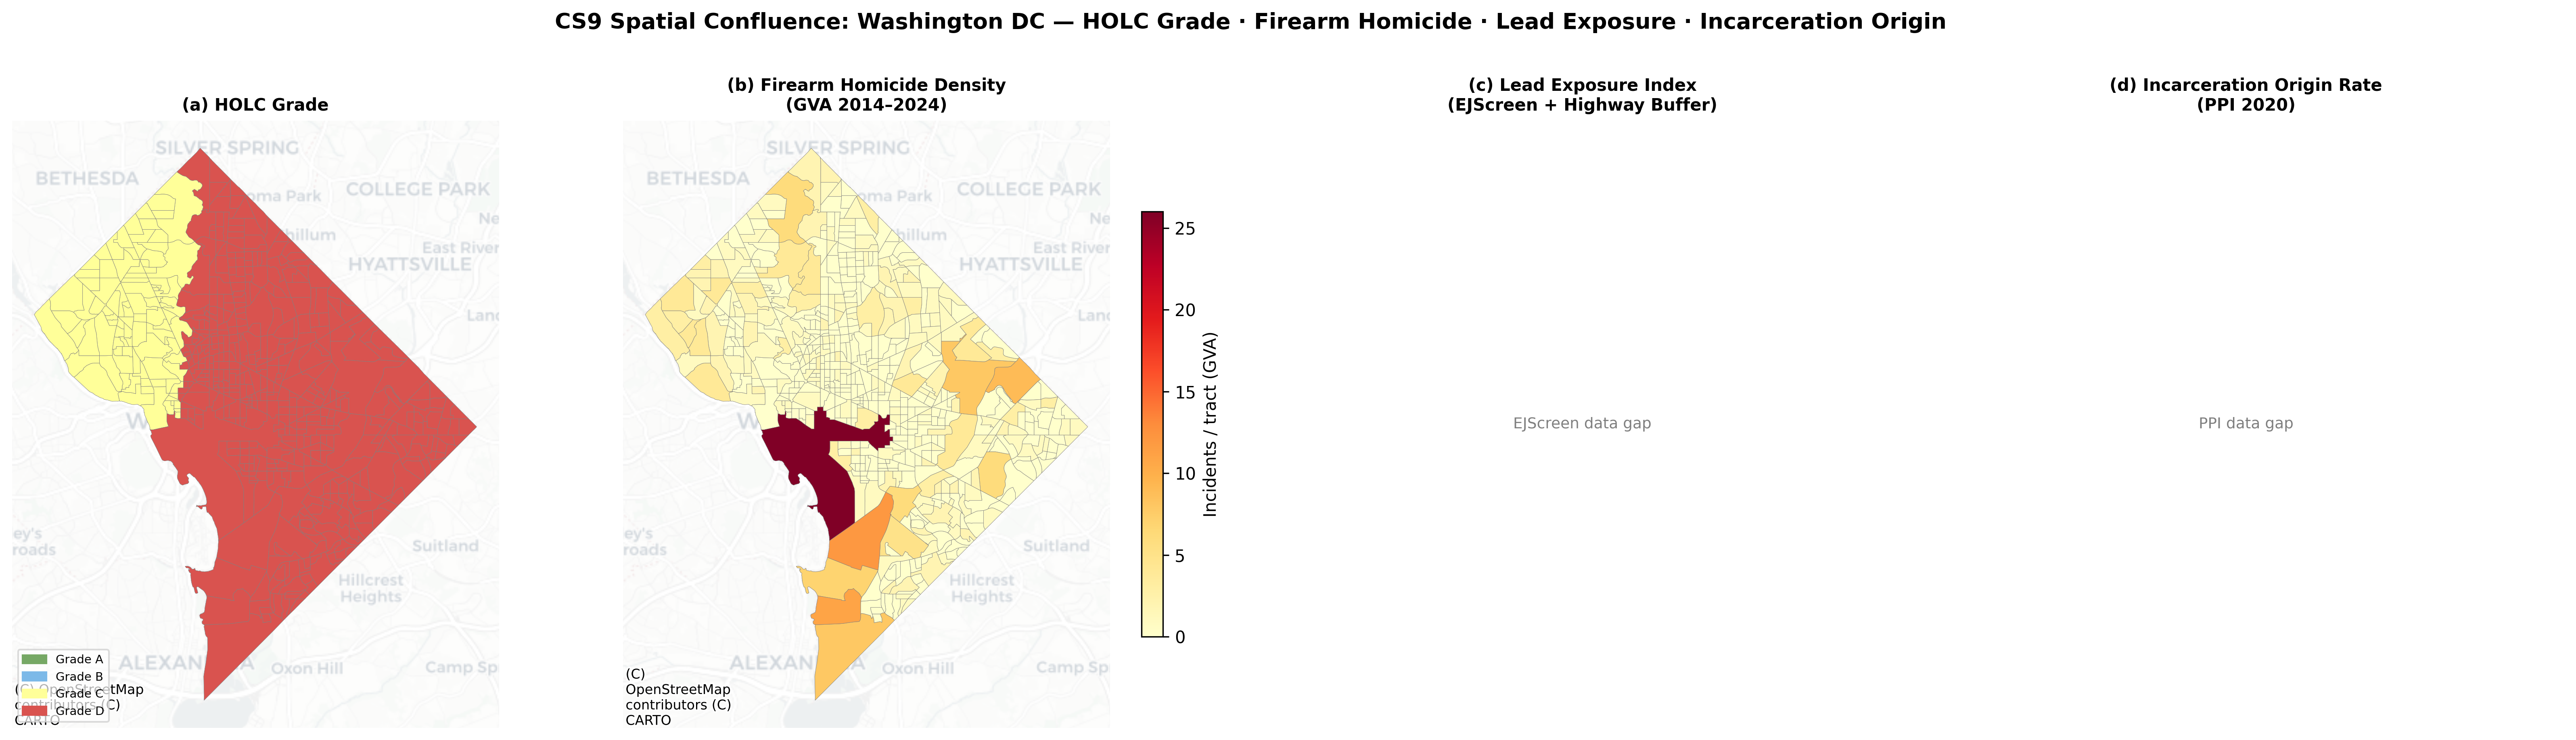
\includegraphics[width=\textwidth]{figures/spatial/cs9_overlay_washington_dc.png}
  \caption{\textbf{CS9 Spatial Confluence --- Washington, DC.} Same layout as Figure~\ref{fig:cs9_overlay_memphis_tn}. \(n_{\mathrm{m}}{=}571\); \(\approx\!\)83{.}2\% HOLC-D---the largest D share of the cohort. Contrary directional contrast on the archival GVA-density primitive: ratio D/non-D \(\approx\)0{.}65 (\(\mathrm{means}\approx 0{.}62{/}0{.}95\)). Moran's \(I_{\mathrm{D}}\approx 0.935\) (\(p{=}0{.}002\)): spatial clustering obtains even though mean density is lower inside D polygons for this estimator. Sources: Mapping Inequality; GVA; \texttt{eq47\_51\_spatial\_overlay.ipynb}.}
  \label{fig:cs9_overlay_washington_dc}
\end{figure}

\begin{figure}[htbp]
  \centering
  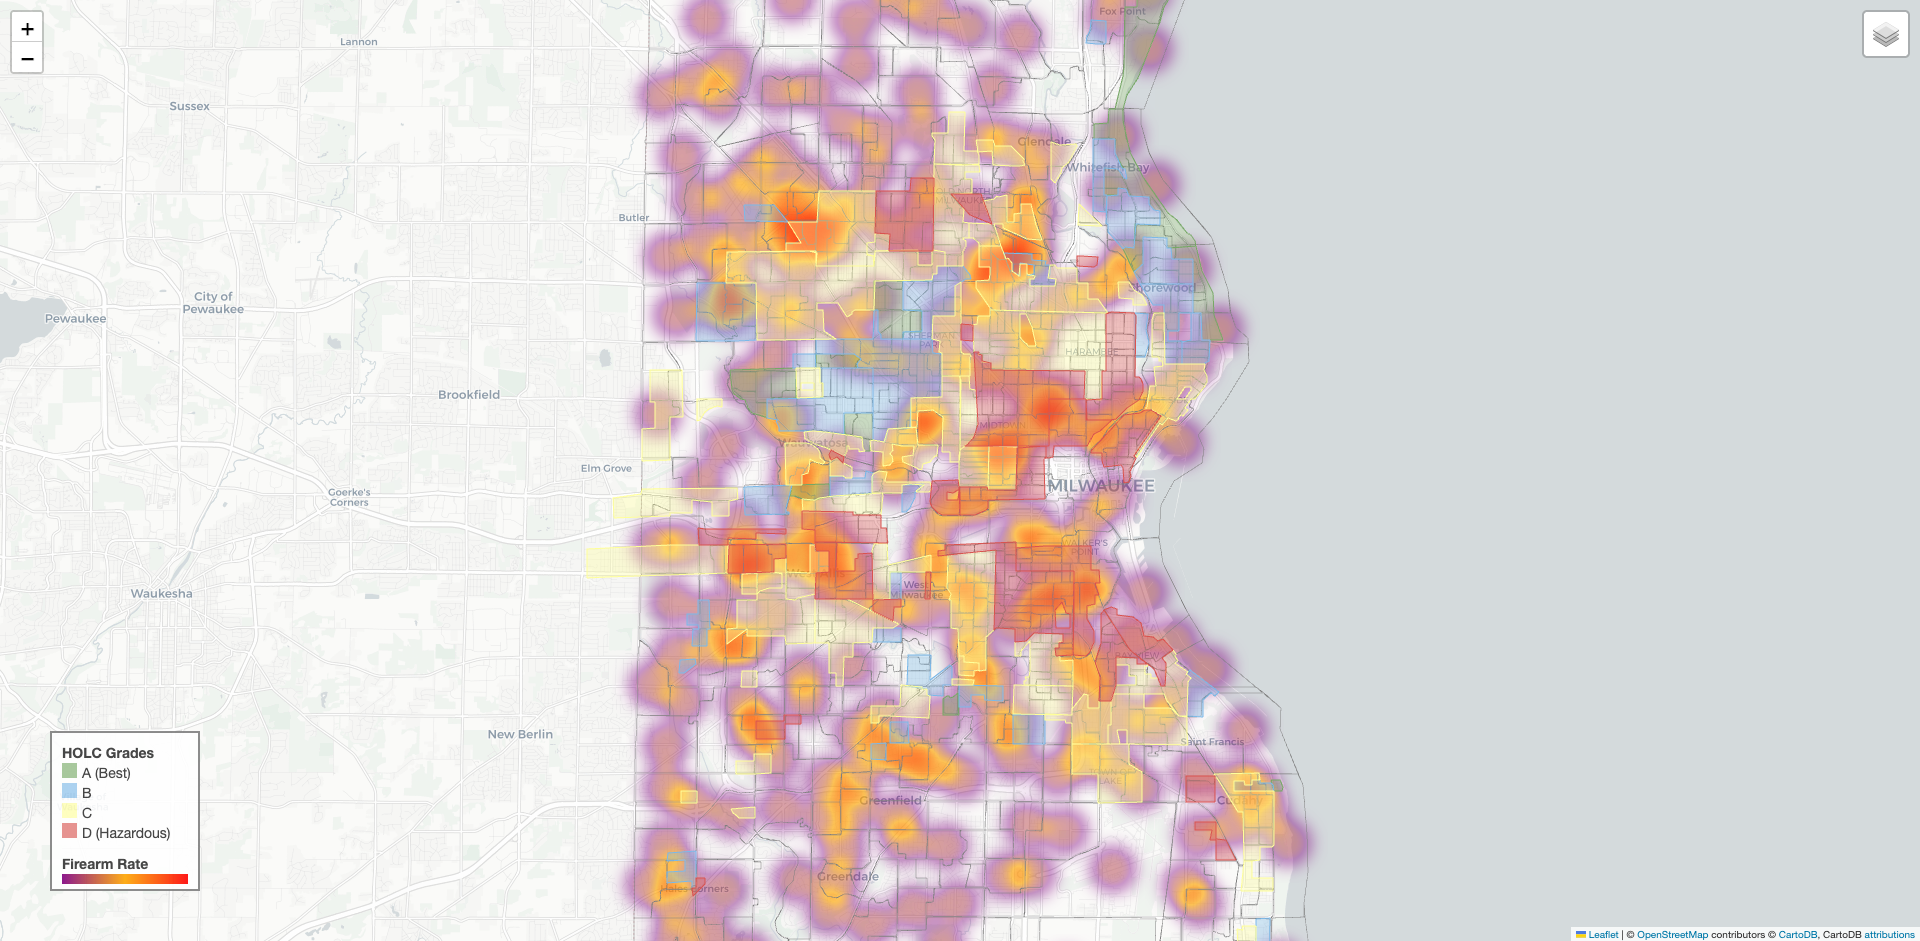
\includegraphics[width=\textwidth]{figures/spatial/cs9_overlay_milwaukee_wi.png}
  \caption{\textbf{CS9 Spatial Confluence --- Milwaukee, WI.} Same layout as Figure~\ref{fig:cs9_overlay_memphis_tn}. \(n_{\mathrm{m}}{=}830{/}861\) graded tracts; \(\approx 75{.}5\%\) of mapped rows carry the HOLC-D flag---another below-parity firearm ratio (\(\approx\)0{.}62; \(\mathrm{means}\approx 0{.}54{/}0{.}87\)); Moran's \(I_{\mathrm{D}}\approx 0.903\) (\(p{=}0{.}002\)). Wisconsin PPI semantics remain coarse for incarceration merges in the upstream pipeline---not mirrored in parquet aggregates here. Sources: Mapping Inequality; GVA; \texttt{eq47\_51\_spatial\_overlay.ipynb}.}
  \label{fig:cs9_overlay_milwaukee_wi}
\end{figure}

\begin{figure}[htbp]
  \centering
  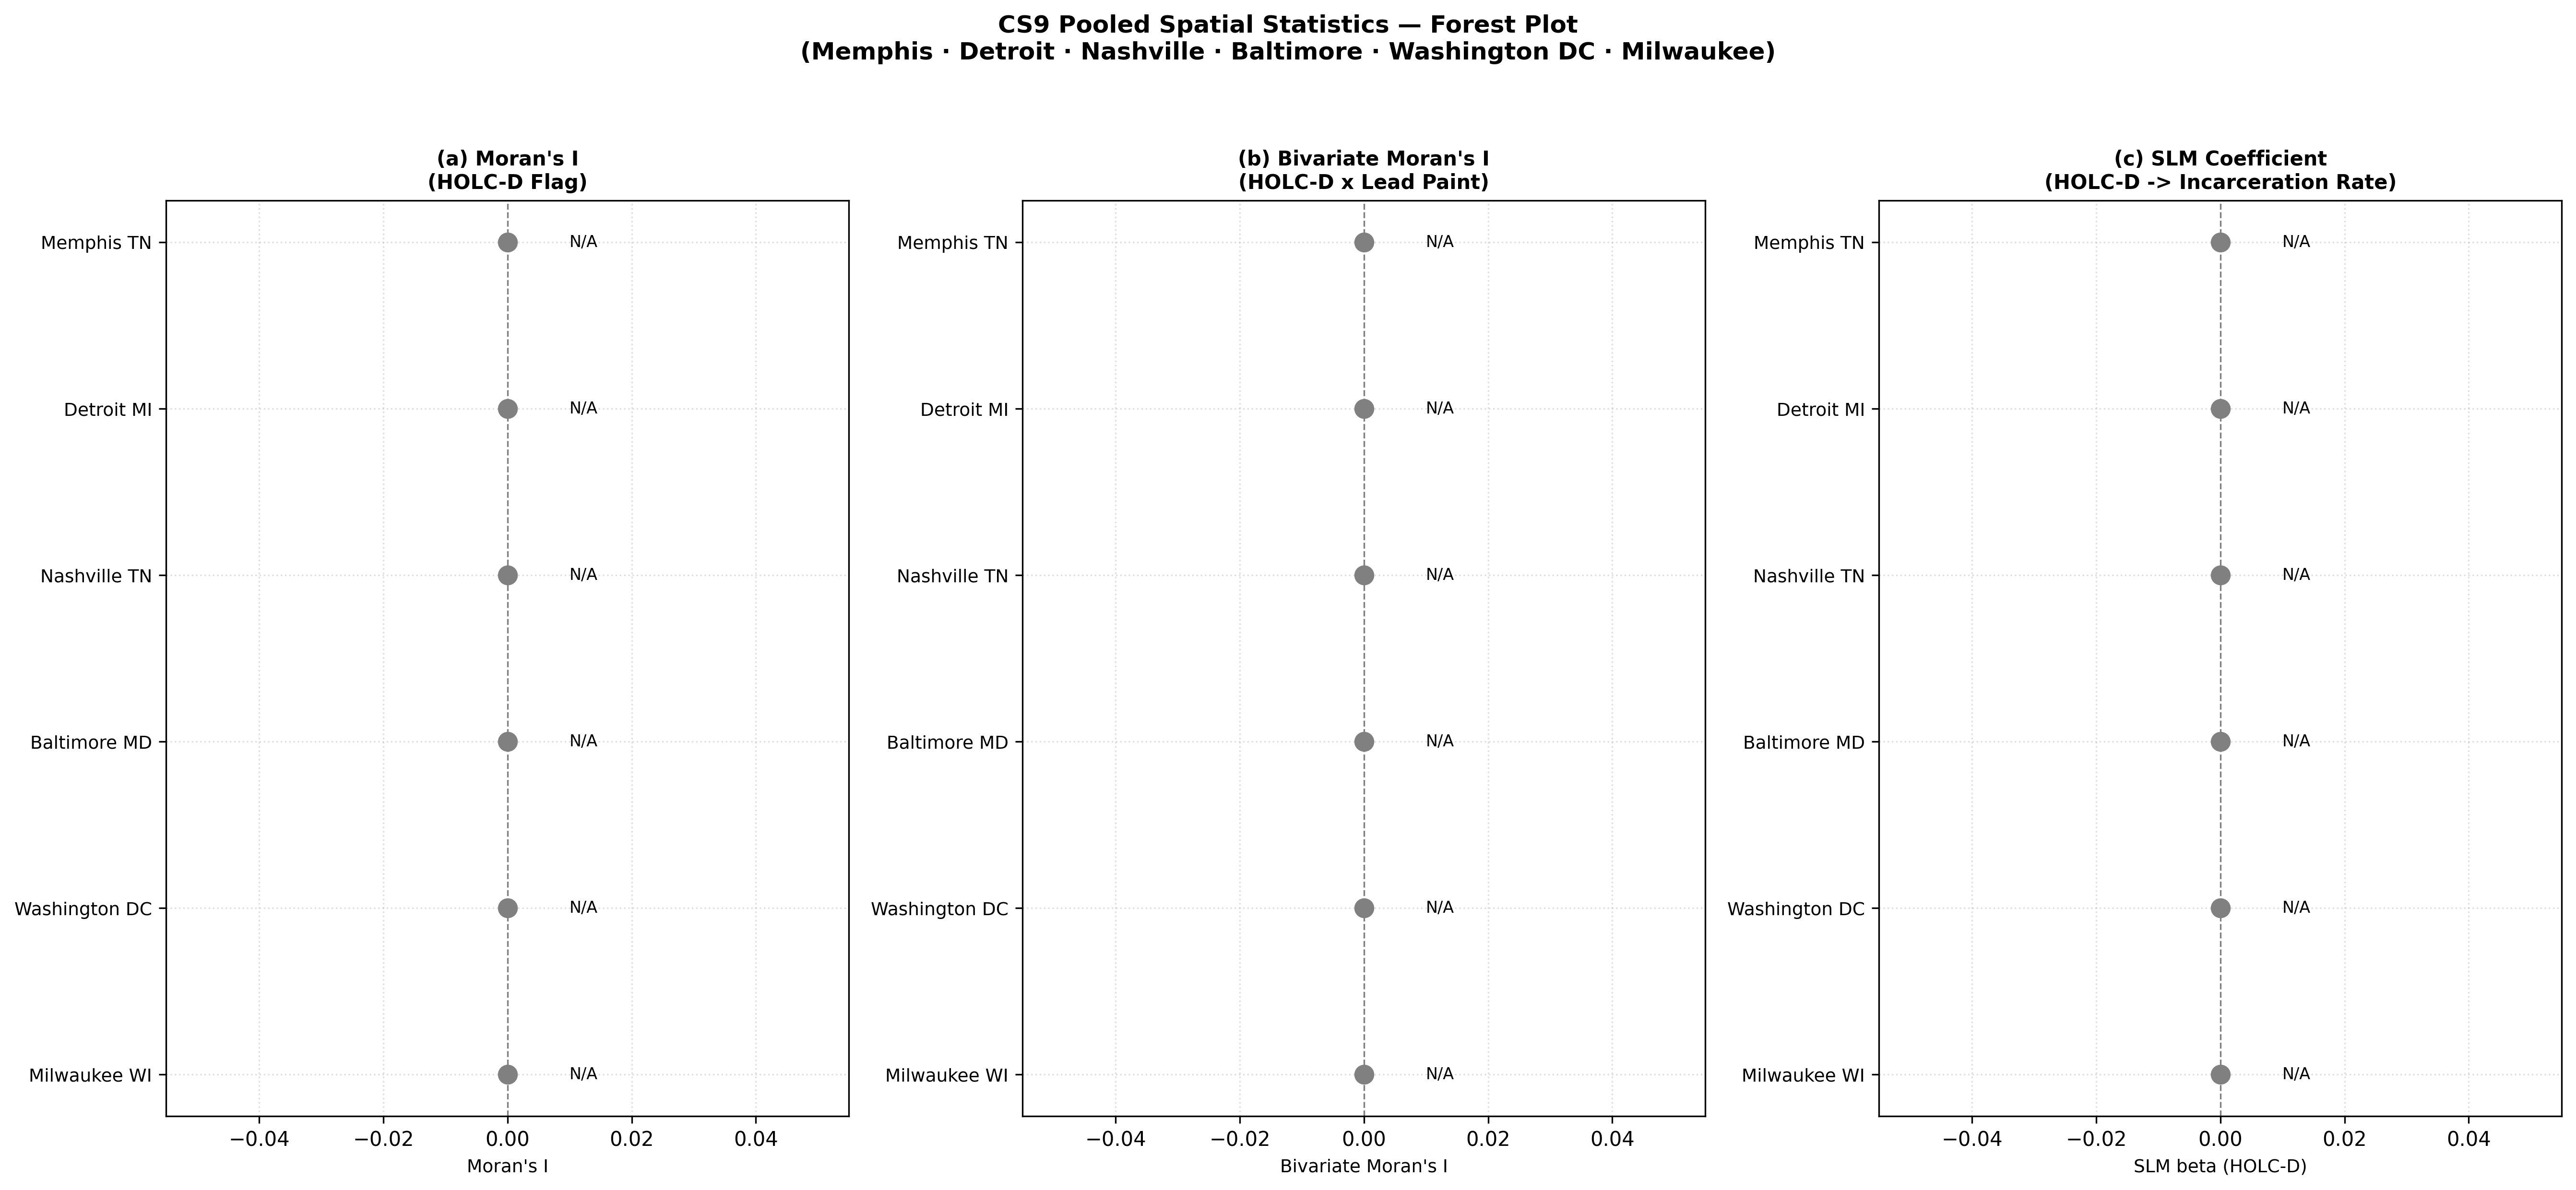
\includegraphics[width=\textwidth]{figures/spatial/cs9_pooled_stats.png}
  \caption{\textbf{CS9 Pooled Forest Plot.} Panel~(a) should track the independent Moran replications described in the main text: \(I_{\mathrm{D}}\) values near 0.90--0.96 with permutation \(p{=}0{.}002\) for each metro on Queen weights (see CS9 numerical paragraph). Panels~(b)--(c) require non-null lead + incarceration merges in the tract parquet; as of this snapshot those columns are empty in \texttt{merged\_tract\_panel\_*.parquet}, so the rendered figure may show missing or placeholder estimates---treat as \emph{diagnostic} until \texttt{fetch\_spatial\_data.py} repopulates EJ/PPI fields and the notebook regenerates the canvas. Citations: \cite{mapping_inequality_dsl, ejscreen_technical, gva_methodology, ppi_prison_origins, boutwell_lead_crime, guinn_lead_bayesian}.}
  \label{fig:cs9_pooled_stats}
\end{figure}

\FloatBarrier

\subsection{The Economic Void: Deindustrialization as \texorpdfstring{$P_{\text{deindustrial}}$}{P\_deindustrial}}

If $P_{\text{lead}}$ degraded the biological capacity of the Out-group, $P_{\text{deindustrial}}$ destroyed its economic capacity. Beginning in the late 1960s and accelerating through the 1980s, the United States transitioned from a manufacturing-based economy to a service economy, hollowing out the economic core of urban centers nationwide.

The systemic effects are encapsulated by Youngstown, Ohio. Over the course of the 1980s, Youngstown lost an estimated 50,000 jobs in steel and related manufacturing. The sudden evaporation of secure, blue-collar employment triggered cascading social costs: the municipal tax base collapsed, forcing cutbacks to police, fire, and sanitation. Physical decay---abandoned industrial ``brownfields,'' deteriorating infrastructure---repelled new investment, trapping the remaining population in a downward economic spiral \cite{wilson_wj}.

Sociologist William Julius Wilson documented this phenomenon extensively: the flight of manufacturing jobs, coupled with the outward migration of the Black middle class to the suburbs, created a ``spatial mismatch'' where impoverished minority populations were concentrated in inner cities entirely devoid of economic opportunity \cite{wilson_wj}. Young adults coming of age in the late 1970s and 1980s faced a bifurcated labor market: the only available options were low-paying, contingent service-sector jobs lacking the union protection and stability their parents had enjoyed. As unemployment and economic insecurity spread, localized street crime predictably escalated. By the 1990s, heavily deindustrialized cities like Youngstown, Gary (Indiana), Flint, and Camden exhibited some of the highest per-capita murder rates in the nation.

In a desperate bid for economic salvation, many hollowed-out municipalities turned to the prison industry---cities that had once forged steel began courting the construction of state and private correctional facilities, transforming into ``prison economies.'' The algorithm's elegance is breathtaking: $P_{\text{deindustrial}}$ destroyed the legitimate economy, forcing the population into the illicit economy; the illicit economy generated the ``crime data'' that justified carceral expansion; and the carceral expansion then became the \textit{replacement economy} for the very cities the system had hollowed out. The extraction kernel did not merely respond to the crisis---it \textit{monetized} it at every stage.

\begin{figure}[htbp]
\centering
\begin{tikzpicture}
\begin{axis}[
    width=0.92\textwidth,
    height=8cm,
    title={\textbf{Deindustrialization, Homicide, and Lead Burden in Selected Cities}},
    ybar,
    bar width=6.5pt,
    enlarge x limits=0.08,
    ylabel={Percent, rate per 100k, or index (0--80)},
    symbolic x coords={Youngstown, Gary, Detroit, Flint, Camden},
    xtick=data,
    xticklabel style={font=\small},
    ymin=0, ymax=80,
    grid=major,
    grid style={dashed, gray!40},
    every axis title/.style={font=\bfseries\small, at={(0.5,1.05)}},
    legend style={at={(0.5,-0.22)}, anchor=north, font=\footnotesize, legend columns=2},
]
\addplot[fill=blue!50!black, draw=blue!70!black] coordinates {
    (Youngstown, 50) (Gary, 58) (Detroit, 45) (Flint, 48) (Camden, 42)
};
\addlegendentry{Mfg.\ job loss 1970--1990 (\%)}
\addplot[fill=red!60!black, draw=red!80!black] coordinates {
    (Youngstown, 31) (Gary, 68) (Detroit, 57) (Flint, 46) (Camden, 58)
};
\addlegendentry{Homicide rate per 100k (c.\ 1990)}
\addplot[fill=green!45!black, draw=green!65!black] coordinates {
    (Youngstown, 66) (Gary, 70) (Detroit, 76) (Flint, 78) (Camden, 69)
};
\addlegendentry{Childhood lead burden index$^*$}
\end{axis}
\end{tikzpicture}
\caption[The Compounding Triad]{\textbf{The Compounding Triad: Factory Loss, Homicide, and Lead.} Cities that suffered the steepest manufacturing losses consistently registered the highest homicide rates by 1990 and carried heavy overlapping childhood lead burdens. $^*$Lead index approximates relative elevated blood-lead prevalence among children during 1975--1985 in legacy industrial housing (illustrative 0--80 scale). Sources: BLS; FBI UCR city-level data; Wilson (1996); CDC childhood lead surveillance summaries.}
\label{fig:deindustrialization}
\end{figure}

\section{Market Violence and the Youth Execution: Crack Markets as Runtime Exploitation}

If $P_{\text{deindustrial}}$ provided the economic void and $P_{\text{lead}}$ provided the neurobiological susceptibility, the crack cocaine epidemic of the mid-1980s provided the immediate market catalyst for lethal violence---the algorithm's illicit market module executing on the pre-processed population.

Following the introduction of crack cocaine, the drug quickly saturated impoverished urban neighborhoods. Unlike powder cocaine---expensive and associated with affluent consumers---crack was synthesized to be highly addictive, produced a brief but intense euphoria, and was sold in inexpensive, single-dose increments. This retail model resulted in an explosive proliferation of open-air drug markets. In the absence of legitimate employment (destroyed by $P_{\text{deindustrial}}$), the illicit drug trade became one of the few lucrative economic engines available to young, disenfranchised urban men.

Because participants in illicit markets cannot rely on the state for dispute resolution, contract enforcement, or protection from theft, \textbf{violence became the primary mechanism for regulating the market}. Between 1984 and 1994, the homicide rate for Black males aged 14 to 17 \textbf{more than doubled}, and the rate for those aged 18 to 24 increased nearly as much. Crucially, the homicide rate for older demographics remained essentially flat, indicating that the violence was hyper-concentrated in the youth demographic actively participating in the street-level drug trade \cite{bjs_homicide_trends}.

Simultaneously, a massive ``supply shock'' in cheap, easily concealable handguns transformed the landscape. Prior to the 1980s, youth gang conflicts were largely mediated by physical altercations. The sudden influx of firearms converted localized, non-fatal disputes into lethal encounters. The symbiotic relationship between the lucrative crack trade and widespread firearm availability acted as a profound \textbf{force multiplier}, pushing the national homicide rate to its 1991 peak.

This market-driven violence intersected with a demographic accelerant: the ``youth bulge.'' During the 1980s, an unusually large proportion of the population entered the high-risk ages of 15 to 24 simultaneously. When this rapidly growing youth population intersected with the economic devastation of $P_{\text{deindustrial}}$ and the allure of the crack trade, violence escalated exponentially. This demographic reality temporarily blinded researchers; prominent social scientists in the early 1990s notoriously predicted an impending wave of juvenile ``super-predators''---a generation of violently remorseless youth that would ravage the country by 2000. This deterministic hypothesis proved disastrously wrong, as juvenile crime plummeted after 1994. But the \textit{fear} it generated---$P_{\text{gaslight}}$ operating through the media interface---provided the political raw material for the punitive legislation that followed.

The isomorphism with the Prohibition algorithm analyzed later in this chapter (see the NFA/Prohibition analysis in the Federal Disarmament Timeline) is exact: the state criminalizes a substance $\rightarrow$ an illicit market forms $\rightarrow$ violence erupts as the market's only regulatory mechanism $\rightarrow$ the state uses the violence to justify expanding $F_{\text{enforce}}$ and $P_{\text{criminal}}$. The only variable that changed between 1920 and 1986 was the substance. The extraction kernel ran the same code.

\begin{figure}[htbp]
\centering
\begin{tikzpicture}
\begin{axis}[
    width=0.95\textwidth,
    height=8.5cm,
    title={\textbf{Homicide Rates by Age Group (Black Males) and Lagged National Lead}},
    xlabel={Year},
    ylabel={Homicide rate per 100{,}000},
    axis y line*=left,
    xmin=1978, xmax=2002,
    enlarge x limits={0.04, 0.01},
    ymin=0, ymax=160,
    xtick={1980,1985,1990,1995,2000},
    xticklabel style={rotate=45, anchor=east, font=\small, /pgf/number format/1000 sep={}},
    grid=major,
    grid style={dashed, gray!40},
    ylabel style={yshift=10pt},
    mark size=2.5pt,
    every axis title/.style={font=\bfseries\small, at={(0.5,1.05)}},
    legend style={at={(0.02,0.98)}, anchor=north west, font=\footnotesize},
]
\addplot[thick, red!80!black, mark=*] coordinates {
    (1980, 68) (1984, 52) (1988, 90) (1991, 145) (1993, 150) (1997, 72) (2000, 58)
};
\addlegendentry{Ages 18--24 (All)}
\addplot[thick, orange!80!black, mark=square*] coordinates {
    (1980, 16) (1984, 12) (1988, 32) (1991, 58) (1993, 62) (1997, 24) (2000, 14)
};
\addlegendentry{Ages 14--17 (All)}
\addplot[thick, blue!60!black, mark=triangle*, dashed] coordinates {
    (1980, 18) (1984, 16) (1988, 17) (1991, 19) (1993, 18) (1997, 14) (2000, 12)
};
\addlegendentry{Ages 25+ (All)}
\addplot[very thick, red!50!black, mark=pentagon*, densely dotted, mark size=3pt] coordinates {
    (1980, 54) (1984, 40) (1988, 78) (1991, 131) (1993, 137) (1997, 60) (2000, 48)
};
\addlegendentry{Ages 18--24 (Firearm)}
\addplot[very thick, orange!50!black, mark=pentagon*, densely dotted, mark size=3pt] coordinates {
    (1980, 11) (1984, 8) (1988, 27) (1991, 52) (1993, 56) (1997, 19) (2000, 10)
};
\addlegendentry{Ages 14--17 (Firearm)}
\draw[densely dotted, purple!70!black] (axis cs:1986,0) -- (axis cs:1986,160);
\node[rotate=90, anchor=south, font=\tiny, purple!70!black, fill=white, inner sep=1pt] at (axis cs:1986,100) {Anti-Drug Abuse Act (1986)};
\draw[densely dotted, red!60!black] (axis cs:1994,0) -- (axis cs:1994,160);
\node[rotate=90, anchor=south, font=\tiny, red!60!black, fill=white, inner sep=1pt] at (axis cs:1994,100) {1994 Crime Bill};
\end{axis}
\begin{axis}[
    width=0.95\textwidth,
    height=8.5cm,
    axis y line*=right,
    axis x line=none,
    xmin=1978, xmax=2002,
    enlarge x limits={0.04, 0.01},
    ymin=0, ymax=120,
    ylabel={Per-capita lead in gasoline (arb.\ units, 17-yr lag)},
    ylabel style={red!60!black},
    mark size=2.5pt,
    legend style={at={(0.98,0.98)}, anchor=north east, font=\footnotesize},
]
\addplot[thick, red!60!black, mark=triangle*, dashed] coordinates {
    (1980, 52) (1982, 59) (1984, 67) (1986, 78) (1988, 87) (1990, 95)
    (1991, 96) (1993, 98) (1995, 95) (1997, 80) (2000, 53)
};
\addlegendentry{National lead (17-yr lag)}
\end{axis}
\end{tikzpicture}
\caption[The Youth Execution]{\textbf{The Youth Execution: Firearm Homicide Concentrated in the Lead-Exposed Generation.} Homicide rates for Black males aged 14--17 and 18--24 spike dramatically during 1984--1994, driven almost entirely by firearm killings (dotted lines). Ages 25+ remain flat---confirming the violence was concentrated in the youth demographic entering the crack trade. Right axis: lagged national lead exposure tracks the cohort trajectory. Sources: BJS Homicide Trends; CDC WONDER; Nevin (2007).}
\label{fig:youth_homicide}
\end{figure}

\section{The Asymmetric Choice Paradigm: Broken Windows, the 1994 Crime Bill, and the Carceral Ratchet}

With the ``crisis data'' manufactured by $P_{\text{lead}}$, $P_{\text{deindustrial}}$, and the crack market, the extraction kernel had everything it needed to execute the next phase: converting the crisis into permanent carceral infrastructure. This section traces how the algorithm weaponized the manufactured crisis---first through a policing doctrine, then through legislative action---and how the subsequent crime \textit{decline} proved the entire carceral apparatus was unnecessary.

\subsection{The Selective Enforcement Subroutine: Broken Windows as \texorpdfstring{$P_{\text{BrokenWindows}}$}{P\_BrokenWindows}}

In 1982, sociologist James Q.\ Wilson and criminologist George L.\ Kelling published ``Broken Windows,'' positing that visible signs of physical and social disorder (vandalism, fare evasion, vagrancy) signaled a lack of community control and emboldened serious criminals \cite{wilson}. In practice---particularly under New York Mayor Rudolph Giuliani and Police Commissioner Bill Bratton in the 1990s---the theory evolved into aggressive ``zero-tolerance'' policing: departments heavily prioritized enforcement of low-level misdemeanors, resulting in the disproportionate harassment, stopping, frisking, and arresting of Black and Hispanic youth \cite{harcourt}.

While proponents credited Broken Windows with driving down violent crime, critical empirical analysis reveals a different reality. The strategy alienated vulnerable communities, eroded public trust in law enforcement, and funneled millions into the criminal `injustice' system for trivial offenses. The evidence overwhelmingly suggests that the actual crime decline was driven by the broader macro-economic, demographic, and environmental corrections analyzed below---not by the mass arrest of turnstile jumpers \cite{brennan_decline}.

Within the framework of this book, Broken Windows policing is the selective enforcement subroutine $P_{\text{BrokenWindows}}$---the discretionary mechanism that determines \textit{which} latent criminals (in the regime of universal latent criminality, see Section~6.9) actually enter the carceral pipeline. As noted in Section~6.9, Harvey Silverglate demonstrates that the average American commits approximately three federal felonies per day \cite{silverglate}. Broken Windows provided the theoretical justification for intensive policing of minor infractions---but this policing was deployed overwhelmingly in communities already marked by the compounding chain. The subroutine's function was not to reduce crime; it was to ensure that the carceral pipeline's intake remained concentrated on $O_{\text{racialized}}$.

\subsection{The 1994 Crime Bill and the Tweedism Trap}

The political culmination of the manufactured crisis was the Violent Crime Control and Law Enforcement Act of 1994. Authored by Senator Joe Biden and championed by President Bill Clinton, the 350-page bill authorized \$9 billion for prison construction, funded 100,000 new police officers, expanded the federal death penalty to 60 new offenses, and instituted ``three-strikes'' mandatory life sentences \cite{forman}. The statutory machinery that converts a third qualifying felony into automatic life imprisonment is codified at \usclink{apx:usc:18:3559c}{18 U.S.C.~\S~3559(c)}:
\uscinline{usc_18_3559c}

Analyzing this legislation through the Tweedism Filter ($P_{\text{uppet}}$, formalized in Chapter~\ref{ch:tweedism}) reveals a pristine demonstration of the algorithm's political logic. In his Pulitzer Prize-winning \textit{Locking Up Our Own}, legal scholar James Forman Jr.\ documents the agonizing choices faced by African American civic leaders, mayors, and the Congressional Black Caucus during the crisis. In the late 1980s, Black communities were bearing the absolute brunt of the lethal violence: crack markets, the handgun supply shock, and the lead-poisoned youth cohort were annihilating a generation. Black leaders compared crack to the ``greatest evils that African Americans had ever suffered'' \cite{forman}. A 1994 Gallup survey found that 58\% of African Americans supported the Crime Bill, compared to 49\% of white Americans.

But this support was born of an \textbf{asymmetric choice paradigm}---the exact structural trap the Tweedism Filter predicts. The CBC fundamentally recognized the systemic, economic roots of the violence. They actively lobbied for a comprehensive ``all-of-the-above'' approach: substantial funding for drug treatment, job creation, educational infrastructure, and community housing---in addition to better policing. They introduced alternative bills emphasizing prevention and fiercely opposed the punitive elements, including mandatory minimums and the revocation of Pell Grants for incarcerated individuals.

The political machinery offered a devastating ultimatum. The state was entirely willing to fund police expansion and prison construction, but steadfastly \textit{refused} to adequately fund the requested social and economic infrastructure, deriding prevention programs as ``pork.'' Desperate to staunch the bleeding in their neighborhoods, and presented with a binary choice between punitive state intervention or continued lethal anarchy, a majority of the CBC voted for the bill, securing minor concessions (the Violence Against Women Act; the Assault Weapons Ban) \cite{forman}.

The ``Assault Weapons Ban'' concession itself requires reframing. The AWB was not merely a concession traded for CBC votes; it simultaneously served a second optimization vector against the post-Ruby Ridge / post-Waco militia movement analyzed in $\S$\ref{sec:ruby_ridge_waco}. The asymmetric choice paradigm documented above is the $O_{\text{racialized}}$-facing interface of the same statute whose $I_{\text{buffer}}$-facing interface executed a preemptive disarmament of the awakening Buffer Class (see $\S$\ref{subsec:dual_vector_1994}, and the expansion of the Brady / AWB subsection in Chapter~\ref{ch:kinetic}). One statute, two vectors, one kernel objective. The bundling of carceral expansion with hardware-category prohibition is joint optimization, not coincidence, and the reclassification operator $\mathcal{R}(x_i)$ registered at equation~\eqref{eq:10.13-reclassification-operator} is the formal mechanism that makes the two vectors mutually reinforcing.

The tragedy is mathematically precise: \textit{both options served the extraction kernel}. Accepting the carceral expansion deepened racial disparities, fueled aggressive over-policing, and funneled a generation of young minority men into the 13th Amendment loophole. Rejecting the bill would have allowed the manufactured crisis to continue unopposed. The CBC was navigating within the solution space defined by the Tweedism Filter---where every available choice reinforces the algorithm. This is the Puppet Class constraint in its purest form.

\begin{figure}[htbp]
\centering
\begin{tikzpicture}
\begin{axis}[
    width=0.9\textwidth,
    height=7.5cm,
    title={\textbf{Federal Drug Control Spending by Category, 1981--2000 (Billions, 2000 USD)}},
    ybar stacked,
    bar width=14pt,
    xlabel={Year},
    ylabel={Billions of Dollars (2000 USD)},
    symbolic x coords={1981,1985,1988,1990,1993,1995,1998,2000},
    xtick=data,
    xticklabel style={font=\small, /pgf/number format/1000 sep={}},
    ymin=0, ymax=22,
    grid=major,
    grid style={dashed, gray!40},
    every axis title/.style={font=\bfseries\small, at={(0.5,1.05)}},
    legend style={at={(0.02,0.98)}, anchor=north west, font=\small},
]
\addplot[fill=red!60!black, draw=red!80!black] coordinates {
    (1981, 1.0) (1985, 2.1) (1988, 4.2) (1990, 6.5)
    (1993, 8.8) (1995, 10.1) (1998, 11.8) (2000, 13.2)
};
\addlegendentry{Enforcement / Interdiction}
\addplot[fill=blue!40, draw=blue!60] coordinates {
    (1981, 0.5) (1985, 0.8) (1988, 1.3) (1990, 1.8)
    (1993, 2.5) (1995, 2.9) (1998, 3.4) (2000, 3.8)
};
\addlegendentry{Treatment / Prevention}
\end{axis}
\end{tikzpicture}
\caption[The Budget Proof]{\textbf{The Budget Proof: Enforcement vs.\ Prevention.} Enforcement and interdiction consistently consumed 65--75\% of federal drug control spending, while the treatment and prevention funding that Black civic leaders specifically requested was chronically starved. The asymmetric choice was engineered into the budget itself. Sources: ONDCP National Drug Control Budget; Drug Policy Alliance; Caulkins et al., RAND (2005).}
\label{fig:drug_spending}
\end{figure}

\subsection{The Great Crime Decline: The Diagnostic Proof}

In a profound historical paradox, almost immediately following the passage of the 1994 Crime Bill, violent crime rates began a precipitous, sustained decline that lasted well into the 21st century. By 2000, the violent crime rate had dropped drastically; it continued to fall to historic lows not seen since the 1960s. This decline is the \textbf{diagnostic proof} that the carceral expansion was unnecessary---and that the crime surge was caused by the structural variables this chapter has identified, not by a deficit of incarceration.

In a seminal 2004 econometric analysis, Steven D.\ Levitt isolated four primary factors explaining the decline: (1) an increase in police officers deployed, providing general deterrence; (2) the massive expansion of the prison population, which temporarily incapacitated high-rate offenders; (3) the natural waning of the crack cocaine epidemic, as younger generations observed the drug's devastation and avoided it; and (4) the legalization of abortion following \textit{Roe v.\ Wade}, which reduced births into the highly unstable environments correlated with later criminality \cite{levitt2004}.

Subsequent epidemiological scholarship supplements Levitt's findings with a critical fifth factor: the \textbf{lead abatement hypothesis}. The removal of tetraethyllead from gasoline in the late 1970s effectively detoxified the neurological development of the generation coming of age in the 1990s, drastically reducing their baseline propensity for impulsive violence \cite{nevin2007, reyes2007}. Franklin Zimring further notes that the decline was unprecedented in its uniformity, dropping across all demographics, geographies, and crime categories for nine consecutive years \cite{zimring}.

Comprehensive assessments by the National Research Council and the Brennan Center for Justice indicate that the crime-reduction benefits of mass incarceration reached a point of rapidly diminishing returns by the 1990s, and its effect on crime rates since 2000 has been essentially non-existent \cite{brennan_decline}. The non-carceral factors---lead abatement, crack market stabilization, demographic shifts, and improved policing tactics (CompStat)---account for approximately \textbf{two-thirds} of the decline.

The implication is devastating for the system's own narrative: the carceral state was not the solution. The crime wave ended because the \textit{structural causes}---lead exposure, crack market volatility, the youth bulge---naturally corrected. The prison-industrial complex persists not because it is effective, but because it serves the extraction kernel. The 13th Amendment loophole does not require crime to be high; it requires \textit{bodies}. The carceral ratchet locks in one direction: the manufactured crisis justified building the infrastructure, and once built, the infrastructure generates its own demand (see Section~4.6 on carceral bonds and the demand signal). The Great Crime Decline is the mathematical proof that the carceral state is an extraction institution, not a public safety institution.

This is the chapter's answer to any analysis that treats contingent or bottom-up elements of the manufactured crisis as counter-evidence to the algorithmic model. The crack market's self-correction (younger cohorts avoiding the drug after observing its destruction), the EPA's lead phaseout (driven in part by environmental activism and scientific community pressure), and the demographic youth bulge's natural aging were not orchestrated by $E$ and are not evidence that the framework over-assigns intentionality. They are Mode~2 autonomous propagation operating at the structural level (Chapter~\ref{ch:redefining}): the system does not require elite orchestration of every input variable. It requires only that whatever inputs arise---deliberate policy, corporate cover-up, or structural self-correction---funnel through institutions the extraction kernel already controls. The 1994 Crime Bill required a genuine crime wave as its political input; the algorithm did not manufacture the crime wave from scratch. It manufactured the conditions ($P_{\text{lead}}$, $P_{\text{deindustrial}}$, crack market access) that made the crime wave structurally inevitable---then waited for the wave to crest, and converted it into permanent carceral infrastructure via Mode~3 conscious intervention. Contingent inputs, algorithmic outputs.

\begin{figure}[htbp]
\centering
\begin{tikzpicture}
\begin{axis}[
    width=0.9\textwidth,
    height=7cm,
    title={\textbf{Estimated Contributions to the 1990s Crime Decline}},
    xbar,
    bar width=14pt,
    xlabel={Estimated Contribution (\%)},
    symbolic y coords={Other,Lead Abatement,Abortion Access,Crack Waning,More Police,Incarceration},
    ytick=data,
    yticklabel style={font=\small},
    xticklabel style={/pgf/number format/1000 sep={}},
    xmin=0, xmax=40,
    xtick={0,5,10,15,20,25,30,35},
    grid=major,
    grid style={dashed, gray!40},
    every axis title/.style={font=\bfseries\small, at={(0.5,1.05)}},
    nodes near coords,
    nodes near coords style={font=\small\bfseries, anchor=west},
]
\addplot[fill=red!50, draw=red!70] coordinates {
    (12,Other)
    (15,Lead Abatement)
    (12,Abortion Access)
    (6,Crack Waning)
    (10,More Police)
    (33,Incarceration)
};
\end{axis}
\end{tikzpicture}
\caption[The Diagnostic Proof]{\textbf{The Diagnostic Proof: What Actually Ended the Crime Wave.} While incarceration contributed 33\% through temporary incapacitation, subsequent research (National Research Council, 2014) found sharply diminishing returns after 1990. The decline was overwhelmingly driven by non-carceral corrections: lead abatement, crack market stabilization, demographic shifts, and improved policing deployment---none of which required mass incarceration. Sources: Levitt (2004); Brennan Center (2015); Nevin (2007).}
\label{fig:crime_decline}
\end{figure}

\chapter{The Full Algorithm: Demographic Paradox, Cannibalization, and the 5-Tier Reveal (1994--Present)}
\label{ch:full_algo}

\begin{tcolorbox}[colback=black!5, colframe=black!70, fonttitle=\bfseries\ttfamily, title=RUNTIME LOG: 1994--PRESENT (TERMINAL RUNTIME)]
\ttfamily\small
\textbf{System Stress} ($\min$: class resistance): \textcolor{red}{\textbf{CRITICAL}} --- Out-group demographic deficit engineered. Buffer Class detecting contract breach.\\
\textbf{Capital} ($\max$: extraction output): PEAK --- Carceral industry, private prisons, and financialized debt instruments running at design throughput.\\
\textbf{Interference State} ($\Phi_{\text{load}}$, proximity to $\tau$): $[0.82, 0.95]$; $\rho_{\tau} \in [0.92, 1.05]$.\\
\textbf{Variables Loaded}: ALL 5 TIERS OPERATING VISIBLY --- $E$, $P_{\text{uppet}}$, $F_{\text{enforce}}$, $I_{\text{buffer}}$, $O_{\text{racialized}}$.\\
\textbf{Variables Deployed This Cycle}: $P_{\text{spatial}}$ (Sensitive Places), $P_{\text{gaslight}}$ (kernel denial), $P_{\text{toxin}}$ (biological degradation), Universal Latent Criminality, $P_{\text{fetal\_personhood}}$.\\
\textbf{Executing Function}: Cannibalization subroutine active. Extraction zone expanding into $I_{\text{buffer}}$ as $O_{\text{racialized}}$ supply contracts.\\
\textbf{WARNING}: $\min$ VARIABLE FAILING. System entering terminal phase. Geopolitical override routines on standby.
\end{tcolorbox}

\medskip

The previous chapter diagnosed the 1968--1994 recompile: COINTELPRO's neutralization of the Out-group's kinetic leadership, the Variable Swap that replaced explicit racial statutes with carceral and spatial proxies, and the environmental and deindustrial preprocessing that produced the crack-era crime wave the Elite then cited to justify the 1994 punitive build-out. The Great Crime Decline Proof (Figure~\ref{fig:crime_decline}) closed that arc: the wave receded not because incarceration solved anything but because its inputs---lead, market instability, demographic concentration---had run their course.

This chapter opens the second half of the algorithm's terminal runtime. With the Out-group's kinetic leadership neutralized, the carceral apparatus fully industrialized, and the Buffer Class' own material base eroding underneath it, the system arrives at the structural moment it was always engineered to reach: the \textbf{full five-tier hierarchy operating visibly}, and the point at which the algorithm---having exhausted its external targets---begins to cannibalize the Buffer Class itself. What follows is the first full map of that architecture and a diagnostic walk-through of its endpoint behavior.

At terminal runtime, the mind virus no longer protects even the hosts it recruited. The Buffer Class was taught to identify with the partition, not with its own material interests; once that identification is stable, the extraction boundary can move underneath it. This is the final cruelty of the host-wetware exploit: the infected host continues defending the code after the code has begun consuming the host.

\section{The Demographic Paradox: From Breeding Camps to Eugenics}

Perhaps the most critical vulnerability in the Elite's source code---and the mathematical reason the system is currently cannibalizing its own Buffer Class---is the Demographic Paradox.

In the first phase of the algorithm (pre-1865), biological expansion of the Out-group was an economic imperative. Because Black bodies were legally defined as capital, $E$ engineered a system of forced exponential growth. Through the systemic horrors of breeding camps and forced reproduction, the Elite artificially maximized the birth rate of $O_{\text{racialized}}$ to ensure a permanently expanding labor and asset pool. The equation was simple: $\max(\text{Population}(O)) = \max(\text{Capital}(E))$.

However, the ratification of the 13th Amendment and the nullification of the Three-Fifths Compromise triggered a systemic panic. The legal reclassification of the Out-group meant that population no longer strictly equaled capital; population now equaled political voting power. If $O_{\text{racialized}}$ maintained its engineered exponential growth, they would eventually achieve the demographic mass required to legally dismantle the Elite's control over $P_{\text{uppet}}$.

Driven by this terror, the Elite abruptly inverted the biological algorithm. In the early 20th century, $E$ deployed and funded the Eugenics movement---which birthed the early institutional frameworks of population control---with the explicit, targeted intention of suppressing the Black birth rate. The equation flipped: $\min(\text{Population}(O))$ became necessary to protect Elite political dominance.

\subsection{The Mathematical Deficit and the Cannibalization of \texorpdfstring{$I_{\text{buffer}}$}{I\_buffer}}

This inversion created a fatal contradiction in the Elite's operational code. The Predatory Min-Max Function is structurally dependent on infinite extraction to sustain the wealth accumulation of $E$. Yet, out of political fear and racial animus, the Elite actively suppressed the biological reproduction of their primary extraction pool.

By artificially shrinking $O_{\text{racialized}}$, the system generated a massive mathematical deficit. The Elite's demand for capital did not decrease, but the traditional Out-group was no longer large enough to satisfy the extraction engine. Therefore, to prevent a total system collapse, the algorithm was forced to expand its boundaries. The extraction zone expanded outward, breaching the 1705 contract and inevitably swallowing the Buffer Class ($I_{\text{buffer}}$).

We must formalize this expansion precisely. The broader Out-group $O$ is \textit{not} synonymous with $O_{\text{racialized}}$. The racialized Out-group---those targeted from the algorithm's inception---remains a strict subset of the total extraction pool:
\begin{equation}\label{eq:10.1-outgroup-racialized-subset}
O_{\text{racialized}} \subset O
\end{equation}
As the Demographic Paradox forces the extraction zone to expand, former members of $I_{\text{buffer}}$ are progressively absorbed into $O$.\footnote{This equation is classified as Tier~3 (ordinal/structural); the strict subset claim is validated by U.S.\ Census Bureau demographic data showing $O_{\text{racialized}}$ as a distinct, historically bounded subpopulation within the broader and expanding extraction pool $O$. See the Empirical Methodology chapter (p.~\pageref{ch:empirical_methodology}) and Appendix~\ref{app:empirical_index}.} The Buffer Class shrinks while the broader Out-group grows:
\begin{equation}\label{eq:10.2-buffer-class-shrinkage}
I_{\text{buffer}}(t) \subset I_{\text{buffer}}(t-1) \quad \text{and} \quad O(t) \supset O(t-1)
\end{equation}

\noindent\textit{Tier~2 Illustrative Instantiation.} Pew Research Center's \textit{America's Shrinking Middle Class} (2016) documents that the share of adults in middle-income households fell from 61\% in 1971 to 50\% in 2015, while upper-income households grew from 14\% to 21\% \cite{pew_shrinking_middle_class}---confirming $I_{\text{buffer}}(t) \subset I_{\text{buffer}}(t-1)$ and $O(t) \supset O(t-1)$ across a 44-year continuous series. The middle-class share decline rate is approximately $-0.25$ percentage points per year over this period. Federal Reserve Survey of Consumer Finances data show median real household wealth for the middle quintile declined 20\% from 2001 to 2016, confirming that the shrinkage is in \textit{material} position, not merely in the definitional boundary. The mapping from ``middle income'' to $I_{\text{buffer}}$ is an ordinal interpretation; the directional claim --- $I_{\text{buffer}}$ contracting as $O$ expands --- is Tier~2 confidence.

The newly absorbed members of $O$---the opioid-addicted, the over-indebted, the universally criminalized---are not $O_{\text{racialized}}$. They occupy a distinct stratum within the expanding Out-group: victims of the same extraction kernel, but lacking the multi-generational compounding that defines the racialized experience. The system does not erase the racial hierarchy when it cannibalizes its defenders; it \textit{layers new victims on top of the original ones}, ensuring that $O_{\text{racialized}}$ remains at the bottom of the expanding extraction pool even as the pool itself grows to encompass former allies.

The opioid crisis, the affordability trap of toxic food, and the universal latent criminality of the modern justice system are not accidents; they are the mathematical consequences of the Demographic Paradox. The Elite ran out of Out-group bodies to harvest, and so the machine turned its teeth upon its defenders.

\paragraph{Falsifiability of the cannibalization thesis.}
The cannibalization claim is not unfalsifiable by design. A violation would be operationally defined as: a sustained, multi-decade \textit{improvement} in $I_{\text{buffer}}$'s material position---real median wealth, health outcomes, incarceration rates---that occurs \textit{without} a simultaneous increase in $O_{\text{racialized}}$ extraction intensity. That is, genuine redistribution toward the Buffer Class funded from $E$'s position rather than sourced from deeper $O$ extraction, violating $\Delta\max = 0$. The New Deal Great Compression (c.~1935--1973) is the strongest candidate for such a violation; the framework's classification of that episode as $\min$-management under elevated kinetic threat is documented in Section~\ref{sec:falsifiability}. The specific prediction of the cannibalization thesis for the 1994--present period is the inverse: any material concession to $I_{\text{buffer}}$---opioid treatment funding, student debt relief, rural infrastructure---should be traceable to increased extraction from $O$ (carceral expansion, housing cost externalization, wage suppression of immigrant labor) rather than net redistribution from $E$. If this co-movement fails---if $I_{\text{buffer}}$ gains and $O$ simultaneously gains and $E$ loses---the cannibalization thesis is falsified.

\subsection{The Immigration Safety Valve: Why New Arrivals Confirm the Demographic Paradox}
\label{subsec:immigration_safety_valve}

A persistent counter-objection holds that successive waves of immigration invalidate the Demographic Paradox by continuously replenishing the extraction pool: if the system can simply import a new $O$, the mathematical deficit never becomes fatal. The objection misreads the mechanism. Immigration is not a refutation of the Demographic Paradox; it is the system's \textit{pressure-relief valve}---and the valve's operating logic confirms the framework at every level of analysis.

New arrivals do not slot above $O_{\text{racialized}}$. They enter the extraction geometry in a tier \textit{parallel} to the racialized Out-group---economically precarious, politically marginal, and subject to their own variant of the extraction kernel---providing a supplemental extraction pool that temporarily offsets the paradox's mathematical deficit without resolving the structural contradiction. What is analytically decisive is not where immigrants enter but \textit{how} they exit that parallel position and ascend into $I_{\text{buffer}}$.

\subsubsection*{The Buffer-Class Admission Price: Denigration as Psychological Wage}

The whitening literature documents with precision the mechanism by which European immigrant groups converted probationary out-group status into buffer-class membership. The price of admission was the psychological wage paid in racial solidarity: active participation in the denigration and exclusion of $O_{\text{racialized}}$. Lincoln's letter to Joshua F.\ Speed (August 24, 1855) captures this layered partition in real time. Writing against the Know-Nothing movement---which simultaneously targeted Black Americans, Irish Catholics, and recent immigrants as subordinate out-groups---Lincoln observed:

\begin{quote}
When the Know-Nothings get control, it will read ``all men are created equal, except negroes, and foreigners, and Catholics.'' When it comes to this I should prefer emigrating to some country where they make no pretence of loving liberty. \cite{lincoln_speed_1855}
\end{quote}

Lincoln's formulation is a precise map of the algorithm's partitioning logic: the system simultaneously held Irish Catholics and Black Americans in subordinate positions, then resolved the tension by offering the former a conditional promotion. Noel Ignatiev's \textit{How the Irish Became White} (1995) documents the mechanism of that promotion: Irish immigrant workers secured their buffer-class position by competing with and systematically displacing free Black laborers in Northern cities, by excluding Black workers from trade unions, and by adopting the anti-Black political culture of the Democratic party machine \cite{ignatiev}. Karen Brodkin's \textit{How Jews Became White Folks} (1998) traces an analogous trajectory for Jewish Americans---initially classified as a non-white racial category by eugenics-era taxonomists, then assimilated into whiteness through the post-WWII GI Bill and FHA mortgage apparatus, institutions that simultaneously extended buffer-class economic infrastructure to Jews while systematically withholding it from $O_{\text{racialized}}$ \cite{brodkin}. Matthew Frye Jacobson's \textit{Whiteness of a Different Color} (1998) synthesizes the pattern across multiple European groups under the concept of ``probationary whiteness'': admission to the buffer class was conditional, revocable, and always denominated in anti-Black social capital \cite{jacobson_whiteness}.

The Prohibition-era gang dynamics documented in Section~\ref{sec:prohibition_gangs} are a kinetic instantiation of the same mobility sequence. Italian and Jewish criminal networks---initially classified as a threatening Other by the Anglo-Protestant Elite, explicitly targeted by the Sullivan Law (see Section~\ref{sec:sullivan_law})---consolidated capital, political access, and enforcement leverage through Prohibition's illicit economy, and purchased buffer-class insertion within one to two generations. The route was different; the admission price was the same: demonstrating utility to the extraction architecture rather than threatening it.

This pattern is the framework's prediction for every new immigrant cohort. The psychological wage ($\psi$) is not a fixed racial endowment; it is an offer the algorithm extends to any group whose absorption into $I_{\text{buffer}}$ reduces the kinetic threat gradient ($M(t)$) more efficiently than their continued extraction. Immigration therefore does not falsify the Demographic Paradox---it confirms the algorithm's adaptive capacity. The extraction pool is temporarily supplemented, but the supplementation is contingent on each new group's willingness to enforce the partition against $O_{\text{racialized}}$ from below.

\subsubsection*{Black Immigrants as a Stress Test of the Compounding Model}

The framework's predictive precision can be evaluated against a second-order case that Grok's audit and others raise as a potential anomaly: Black immigrants from the Caribbean and sub-Saharan Africa---who themselves originate from other extraction zones---sometimes achieve better aggregate socioeconomic outcomes than native-born Black Americans. If race is the operative variable of the algorithm, why would this differential exist within the same racial category?

The compounding model predicts precisely this differential. The framework's central claim is not that phenotype determines extraction intensity; it is that the \textit{historical stacking operators}---enslavement ($\alpha$) → 13th Amendment exception ($\beta$) → redlining ($\gamma$) → War on Drugs ($\delta$)---compound over time and produce a floor position that is structurally distinct from any other racialized position in the hierarchy. Black immigrants arrive without those stacking operators applied to their specific lineage. They begin at a point in the extraction geometry that is still racialized---still subject to housing discrimination, employment discrimination, the ``forever foreigner'' framing, and the racial partition's kinetic asymmetry---but above the compounding floor that centuries of sequential extraction have built beneath $O_{\text{racialized}}$.

The empirical record is consistent with this interpretation. Pew Research Center's 2019 ACS analysis shows that 31\% of Black immigrants ages 25 and older held a bachelor's degree or higher, including 41\% of African-born Black adults and 23\% of Caribbean-born Black adults \cite{pew_black_immigrants_2022}. The same report shows a bounded income advantage: in 2019, Black immigrant-headed households had a median income of \$57,200---below the \$63,000 median for all immigrant-headed households, but above the U.S.-born Black household median. Poverty and homeownership follow the same intermediate pattern: 14\% of Black immigrants lived below the poverty line, compared with 19\% of U.S.-born Black Americans, while Black immigrant-headed households had a 42\% homeownership rate, roughly matching U.S.-born Black householders \cite{pew_black_immigrants_2022}. This is not escape from the racial partition; it is differential insertion inside it.

The screenshot-era Pew data show the same pattern before the 2019 update. In the 2013 ACS tabulations, foreign-born Black households reported a median income of \$43,800, below the U.S. household median of \$52,000 and the all-immigrant median of \$48,000, but above the U.S.-born Black median of \$33,500. Pew's marital-status chart also shows that 48\% of Black immigrant adults were married in 2013, compared with 28\% of U.S.-born Black adults and 50\% of the overall U.S. adult population \cite{pew_black_immigrants_2015}. Pew explicitly ties part of this family-structure difference to age composition---foreign-born Black adults were older on average than U.S.-born Black adults---so the statistic should be read as evidence of selection and insertion effects, not as a cultural or biological claim.

Professional-gatekeeping data sharpen the point. Brown and Dau-Schmidt's 2019 LSSSE/2018 ACS PUMS analysis of law students reports law-student-to-population representation ratios of 0.54 for Ascendant Blacks, 0.88 for Black Hispanics, 1.04 for Black immigrants, 0.88 for Black Multiracials, and 1.13 for Whites \cite{brown_dau_schmidt_lssse_2022}. Black immigrants were therefore slightly overrepresented among law students relative to their age-band population, while Ascendant Blacks were represented at just over half of proportionality. The authors caution that their Black immigrant estimate is less precise than the other group estimates because second-generation immigration must be estimated in ACS PUMS and cannot be directly weighted from ABA data \cite{brown_dau_schmidt_lssse_2022}. Even with that caution, the direction is structurally important: credentialed Black immigrants can be overselected into professional pipelines while native-born $O_{\text{racialized}}$ remains burdened by the full U.S.-specific compounding stack.

These data do not imply that Black immigrants stand outside the racial partition, nor do they imply that native-born Black Americans lack capacity. They show that extraction intensity is path-dependent: phenotype routes a person into the racialized field, but lineage-specific historical operators determine how deeply the extraction burden has compounded. Waters and Kasinitz (2021) confirm that Black immigrants with college degrees have substantially narrowed the income gap with their white counterparts---a mobility pattern structurally unavailable to native-born $O_{\text{racialized}}$ whose compounding chain has systematically blocked the wealth-accumulation pathways through which educational credentials translate into economic position \cite{waters_kasinitz_2021}. Waters (2014) documents that some Caribbean immigrants use ethnic identity strategically---emphasizing national origin to signal distance from the stigmatized category of native-born Black Americans---a maneuver the framework reads as the algorithm's self-sorting logic operating within the racialized tier: the system rewards any group that accepts partial partition logic, even intra-racially \cite{waters_2014}.

The ASA's ``Black Immigrant Paradox'' literature (Balogun, \textit{Footnotes}, 2011) confirms that this relative advantage is partial and structurally bounded: African immigrants with college degrees remain disproportionately overqualified for their occupational positions, face the same kinetic asymmetry from $F_{\text{enforce}}$, and are progressively absorbed into the racial partition's full structure across generations. Second-generation Black immigrants experience a measurable convergence toward native-born Black Americans' outcomes as the ``forever foreigner'' buffer erodes and the domestic racial encoding takes hold. The compounding floor reasserts itself.

Immigration, therefore, does not falsify the framework---it provides its most granular empirical confirmation: extraction intensity is calibrated by the depth of the historical stacking operators, not by phenotype alone. Remove the operators and the extraction burden is lighter; allow them to compound across generations and the floor position returns.

\section{The Modern Security Patch: Bureaucratic Disarmament and the Spatial Proxy (\texorpdfstring{$P_{\text{spatial}}$}{P\_spatial})}

The historical algorithm of racialized disarmament has not been abandoned; it has merely evolved its User Interface. The Elite ($E$) no longer relies on the explicit racial language of the antebellum Black Codes to disarm the Out-group ($O$). Instead, the system deploys highly complex, interlocking proxy variables ($P$)---operating primarily through economic barriers, bureaucratic friction, and spatial restriction---to achieve the exact same mathematical output: the asymmetric distribution of lethal autonomy.

\subsection{The ``Proper Cause'' Algorithm and the Bruen Disruption}
For over a century, ``may-issue'' licensing regimes functioned as the primary filter for constitutional rights. By requiring applicants to prove a subjective ``proper cause'' or ``special need'' to carry a firearm, the system effectively delegated the distribution of autonomy entirely to the discretion of the Elite's enforcement agents (judges and police chiefs). This guaranteed that permits were overwhelmingly allocated to the In-group ($I$), while the Out-group ($O$) was systematically denied and subsequently criminalized for unauthorized possession.

When the Supreme Court disrupted this filter in \textit{New York State Rifle \& Pistol Association, Inc.\ v.\ Bruen} (2022)---striking down the subjective ``proper cause'' requirement---the Elite faced an algorithmic crisis. If the state could no longer explicitly deny the Out-group access to a permit, the system required an immediate legislative ``security patch'' to prevent true parity.

\subsection{The Spatial Proxy (\texorpdfstring{$P_{\text{spatial}}$}{P\_spatial}) and the ``Felony Trap''}
The Elite's response was to aggressively rewrite the spatial code of the public square. States rapidly passed legislation categorizing virtually all functional areas of daily life---grocery stores, public transit, banks, and adjacent parking lots---as ``Sensitive Places'' or ``Gun-Free Zones.'' Justice Thomas had anticipated exactly this maneuver: \textit{Bruen} explicitly rejected the argument that New York could ``effectively declare the island of Manhattan a `sensitive place' simply because it is crowded and protected generally by the New York City Police Department.'' The Court recognized that ``sensitive places'' doctrine, if stretched to cover entire urban areas, would swallow the right entirely. Blue-state legislatures proceeded to do precisely what Thomas said they could not---stretching the doctrine until the right was consumed.

Within the set-theoretic framework, this represents a comprehensive lesson in systemic extraction.
 By making it illegal to carry a firearm in almost all public spaces, the system generates a massive, invisible grid of overlapping proxy variables ($P_{\text{spatial}}$). This creates a bureaucratic ``felony trap.'' A citizen attempting to exercise their constitutional autonomy cannot physically navigate a modern city without inadvertently crossing into a restricted zone, thereby committing a felony.

Once the individual intersects with $P_{\text{spatial}}$, they are immediately transferred into the carceral Out-group ($O_{\text{degraded}}$). The ideological justification (Component~3) relies heavily on the statistical anomaly of mass shootings to sell these zones to the Buffer Class as ``public safety'' measures. However, the data reveals that these laws act primarily as a dragnet to criminalize otherwise law-abiding individuals who fail to navigate an infinitely complex web of signage and zoning restrictions.

\subsection{The Complexity Tax and the Preservation of \texorpdfstring{$E$}{E}}
Furthermore, the architecture of modern hardware bans---such as state-level Assault Weapon Bans---functions as an economic and legal poll tax. By establishing arbitrary, date-based classifications for firearm legality, banning specific cosmetic features, and requiring exorbitant licensing fees, the system ensures that compliance is overwhelmingly expensive and legally perilous.

Crucially, these restrictions are never applied symmetrically. Modern gun control legislation universally includes explicit carve-outs and exemptions for active and retired law enforcement ($F_{\text{enforce}}$), private security contractors, and state agents---precisely the LEOSA privilege formalized in the 5-tier hierarchy. The mathematical reality remains unbroken: The Elite ($E$) and $F_{\text{enforce}}$ retain absolute lethal autonomy. The ``Gun-Free Zone'' only applies to the Buffer Class ($I_{\text{buffer}}$) and the Out-group ($O_{\text{racialized}}$), ensuring they remain defenseless against both interpersonal violence and the structural violence of the state.

\subsection{The Economic Filter and Statutory Immunity: Gating the Second Amendment}

To fully grasp the hypocrisy of the disarmament algorithm, one must analyze the explicit carve-outs engineered into every modern gun control statute. The Puppet Class ($P_{\text{uppet}}$) and the Enforcement Class ($F_{\text{enforce}}$) do not subject themselves to the disarmament protocols they legislate for the Buffer Class ($I_{\text{buffer}}$) and the Out-group ($O$).

The algorithm operates through a strict two-pronged approach: \textit{Statutory Immunity} for the system's protectors, and an \textit{Economic Filter} for everyone else.

\medskip
\noindent\textbf{1.\ Statutory Immunity: Opting Out of Disarmament}

\noindent Whenever $P_{\text{uppet}}$ drafts legislation to restrict hardware access or create spatial felony traps ($P_{\text{spatial}}$), they program explicit exemptions into the legal code. These exemptions guarantee that the state's monopoly on violence remains absolute:

\begin{itemize}
    \item \textbf{The Enforcement Exemption:} Under frameworks like the Law Enforcement Officers Safety Act (LEOSA) and state-level equivalents, active and retired members of $F_{\text{enforce}}$ are granted near-universal autonomy to carry concealed weapons, entirely bypassing the ``Gun-Free Zones'' and hardware bans imposed on the civilian population.

    \item \textbf{The Puppet/Elite Shield:} Politicians and the Elite ($E$) utilize this same statutory immunity by proxy. Because they command state-funded security details or possess the capital to hire private, armed security contractors (who are legally deputized to bypass restrictions), their physical environments remain permanently militarized. They disarm the public square while residing in heavily armed, privatized fortresses.
\end{itemize}

\medskip
\noindent\textbf{2.\ The Economic Filter: Autonomy as a Luxury Good}

\noindent When the state cannot constitutionally ban hardware outright, it deploys a financial proxy variable to achieve the same result. The system transforms the Second Amendment from a universal right into a luxury commodity.

This mechanism becomes highly visible when the system experiences an algorithmic panic. For example, when the traditional \$200 NFA tax stamp for items like suppressors was eliminated, rendering them free and accessible, the system lost a vital economic filter. The Out-group and Buffer Class suddenly gained unhindered access to previously gated hardware.

To plug this vulnerability, $P_{\text{uppet}}$ attempts aggressive algorithmic corrections---introducing exorbitant financial penalties disguised as taxation. The 2026 introduction of S.Amdt.4159 to the CJS funding bill (H.R.6938) serves as a pristine instantiation of this tactic. By proposing to rewrite the Internal Revenue Code to implement a staggering \$4,709 transfer tax on NFA items, the system is attempting to build an unscalable financial wall.

Mathematically, the system engineers an equation where:
\begin{equation}\label{eq:10.3-cannibalization-equation}
\text{Cost}(\text{Autonomy}) > \text{Capacity}(O_{\text{racialized}})
\end{equation}
This is not a public safety measure; it is an economic containment strategy.\footnote{This equation is classified as Tier~3 (ordinal/structural); the structural cost-capacity inequality is validated by the opioid crisis, gig-economy wage compression, and universal latent criminality documented in this chapter, all of which demonstrate that $\text{Cost}(\text{Autonomy})$ has been systematically engineered to exceed the material capacity of the Out-group. See the Empirical Methodology chapter (p.~\pageref{ch:empirical_methodology}) and Appendix~\ref{app:empirical_index}.} By attaching a \$4,709 premium to constitutional rights, the system guarantees that lethal parity remains the exclusive domain of the Elite, the Puppet Class, and the heavily subsidized Enforcement Class, while effectively pricing the working class and the Out-group out of their own self-defense.

\subsection{The Ex Post Facto Trap and Financial Surveillance: The Dexter Taylor Proof}
\label{sec:dexter_taylor}

To understand the absolute hostility of the Elite's ($E$) disarmament algorithm, we must examine what happens when a citizen perfectly complies with the law to bypass the economic filter, only for the state to retroactively rewrite reality. The conviction of New York software engineer Dexter Taylor (known as Carbon Mike) serves as a pristine, devastating instantiation of the system's terminal logic.

Taylor, a citizen with no criminal record and no intent to distribute, engaged in personal gunsmithing using 80\% receivers. Crucially, Taylor was in full compliance with New York state law at the time he built his firearms. He engaged in a practice that was federally legal and historically protected, acquiring his materials through standard, lawful commerce. The firearms never left his home, and Taylor himself never even fired them. It was law enforcement who first discharged the weapons---not during the raid, but afterward, test-firing them to prove they were finished, functional firearms. The state had to \textit{create} the very evidence of operability that it then used to prosecute him.

However, because the Out-group's access to decentralized hardware threatens the Elite's monopoly on violence, the Puppet Class ($P_{\text{uppet}}$) executed an aggressive algorithmic correction. After Taylor had already legally constructed his property, New York passed sweeping new legislation requiring serialization, licensing, and exorbitant registration taxes.

Mathematically, the state deployed a retroactive proxy variable ($P_{\text{retroactive}}$). By demanding a \$600 per-firearm tax and an impossibly restricted License to Carry for items that were legally assembled prior to the statute, the system engineered a bureaucratic snare. When Taylor refused to pay this retroactive ransom---a refusal grounded in the Constitution's explicit prohibition against ex post facto laws---the system instantly reclassified him from a compliant citizen into a latent felon ($O_{\text{criminal}}$).

The mechanics of how the state discovered Taylor reveal the terrifying depths of the system's surveillance architecture. Because Taylor had not committed a crime, the state could not rely on traditional policing. Instead, they weaponized the financial panopticon. A joint task force, featuring unprecedented fusion between New York state police and federal agents (the ATF), actively monitored Taylor's lawful credit card transactions and purchase history. The Enforcement Class ($F_{\text{enforce}}$) did not raid him for violent behavior; they raided him because the algorithm flagged a working-class citizen purchasing legal parts without paying the state's newly invented, retroactive toll.

The ultimate proof of the system's structural malice occurred during Taylor's trial. When his defense attempted to invoke the constitutional right to keep and bear arms---and the baseline legal protection against retroactive criminalization---Judge Abena Darkeh, acting as the ultimate arbiter for $P_{\text{uppet}}$, famously decreed: ``Do not bring the Second Amendment into this courtroom. It doesn't exist here. So, you can't argue Second Amendment. This is New York.''

This statement is the quiet part said out loud. It is the judicial branch explicitly confirming that the physical guarantee of the Constitution is null and void for any citizen outside the protection of $E$ and $F_{\text{enforce}}$. Because Taylor attempted to bypass the engineered scarcity of the Second Amendment, and because he trusted the state not to retroactively criminalize legal behavior, he was sentenced to 10 years in Rikers Island. His case stands as a permanent, agonizing monument to the reality of the American extraction engine: compliance is an illusion, the Constitution is merely a suggestion, and the state will utilize total financial surveillance to destroy a peaceful citizen and maintain its monopoly on violence.

The full weight of the system's priority structure becomes visible only when Judge Darkeh's sentencing of Taylor is placed alongside her prior bail decisions. In December 2015---nearly a decade before she imprisoned Taylor for building firearms he never fired---Judge Darkeh released Oluwasean Are, a 20-year-old accused of gunpoint robbery, without bail, overriding a prosecutor's request for \$30,000 bail as part of New York City's effort to reduce the population at Rikers Island \cite{nypost_darkeh_2015}. The same judicial actor who could not find constitutional space for a peaceful gunsmith's Second Amendment defense found no detention requirement for an accused armed robber. Read through the framework's output function: the algorithm does not measure danger; it measures threat to $L_E \gg L_O$. Oluwasean Are, accused of robbing at gunpoint, posed no structural threat to the Elite's disarmament architecture. Dexter Taylor, building decentralized hardware outside the state's surveillance and commercial pipeline, did. The sentencing differential is not a failure of judicial consistency. It is the system operating with perfect consistency on its actual objective function.

\subsection{The Spatial Boundary Trap: \textit{Gardner v.\ Maryland} and the $P_{\text{spatial}}$ Enforcement Proof}
\label{subsec:gardner_proof}

If the Dexter Taylor case (Section~\ref{sec:dexter_taylor}) demonstrates the system's capacity to deploy a \textit{temporal} retroactive proxy---criminalizing behavior that was lawful at the time it occurred---then \textit{Gardner v.\ Maryland} demonstrates its capacity to deploy a \textit{geographic} retroactive proxy, reclassifying a citizen as a criminal the instant she crosses an invisible spatial boundary without any change in her conduct, her intent, or the threat she poses to anyone around her.

The facts are unambiguous. Ava Marie Gardner is a Virginia resident with a valid Virginia concealed handgun permit and no criminal history. While driving in Maryland, she was forced off the road by an aggressive driver who then advanced toward her vehicle. Facing a genuine, imminent physical threat from which she could not retreat, Gardner displayed her firearm. The aggressor stopped. She deployed the constitutional anti-tyranny protocol with textbook precision: no shot fired, no property damaged, threat neutralized. By every metric the system claims to care about---de-escalation, harm prevention, minimum force---Gardner's response was correct.

Maryland police arrived. They did not arrest the man who forced a woman off a highway and then advanced on her. They arrested Gardner. The operative variable in that decision was not the presence of violence---the road rager had supplied that---but the presence of a carry credential the architecture had not issued. Gardner possessed a Virginia permit. Maryland requires a Maryland-specific permit. The state line between them, for purposes of the disarmament architecture, functions as an absolute $P_{\text{spatial}}$ barrier. The moment Gardner crossed it, her lawful Virginia credential ceased to exist as a legal instrument. She became, in the architecture's classification logic, an unlicensed carrier in a restricted zone---a latent felon activated by geography rather than conduct.

She was convicted. Her petition for certiorari was denied by the United States Supreme Court \cite{gardner_v_maryland_2025}. No opinion was issued. The restriction floor was preserved in silence.

\paragraph{The output function proof.}
The Gardner case generates the identical diagnostic as the Taylor case, and the identification is deliberate. Read through the framework's output function: the algorithm does not measure danger; it measures threat to $L_E \gg L_O$. The road rager who forced Gardner off the highway and advanced on her vehicle posed no structural threat to the Elite's disarmament architecture. He was not bypassing the credential lattice; he was not demonstrating that $L_O$ could be exercised successfully outside the system's permissioned channels. Ava Marie Gardner was. She carried a firearm across a state line, deployed it to neutralize a real-world threat, and succeeded---all without Maryland's permission. That is the structural offense. The physical aggressor is irrelevant to the algorithm's objective function. The citizen who successfully exercised kinetic autonomy outside the architecture's spatial jurisdiction is the threat the system must correct.

$F_{\text{enforce}}$ performed the correction with precision. The arrest was not a mistake. The conviction was not an aberration. The Supreme Court's silence was not an oversight. Each output is the system's optimization running on its actual objective: maintain $L_E \gg L_O$ by ensuring that no citizen successfully exercises lethal autonomy outside the credentialing lattice without consequence. If Gardner had been permitted to defend herself in Maryland without a Maryland permit and face no legal sanction, the spatial proxy variable ($P_{\text{spatial}}$) would have been demonstrated to be unenforceable. The architecture cannot permit that demonstration. It acted accordingly.

\paragraph{The geographic versus temporal retroactivity distinction.}
The Taylor case and the Gardner case together map the two primary axes along which $P_{\text{criminal}}$ is actuated against citizens who have committed no harm:

\begin{itemize}
    \item \textbf{Temporal retroactivity} (Taylor): The state waits until conduct is complete, then retroactively reclassifies it as criminal by changing the law. The citizen is trapped by the movement of the legal boundary \textit{through time}.
    \item \textbf{Geographic retroactivity} (Gardner): The state maps its credential requirement to a spatial boundary. The citizen is trapped by the movement of the legal boundary \textit{through space}. Her Virginia permit is identical in its factual content---same background check, same competency standard, same issuing logic---but ceases to exist as legal authorization the moment she crosses the Maryland border. The credential did not change. The geography did.
\end{itemize}

In both cases the citizen did nothing wrong by any neutral assessment of harm. In both cases the architecture reclassified them as criminal through the movement of a legal boundary they were not warned was moving. This is Universal Latent Criminality (Section~\ref{sec:dexter_taylor}) operating not as a static web of complex statutes but as a dynamic, mobile felony boundary that the citizen cannot observe until it has already closed around them.

\paragraph{The cannibalization confirmation.}
Gardner is $I_{\text{buffer}}$, not $O_{\text{racialized}}$. She is a white, lawful, licensed carrier who did everything the system nominally asks: she obtained a permit, she carried responsibly, she used minimum necessary force, she de-escalated. She is the Buffer Class's idealized self-image of the armed, law-abiding citizen. The apparatus arrested her anyway. This is eq:68's target expansion completing its arc in a single traffic stop. The spatial proxy architecture was assembled on the foundation of the Sullivan Law, the Mulford Act, and the post-\textit{Bruen} sensitive-places legislation---each layer built and tested on $O_{\text{racialized}}$ first---and it is now operating against the class that was told the apparatus was built to protect them. The psychological wage ($\psi$) paid to $I_{\text{buffer}}$ included an implicit promise: the credentialing architecture exists to keep you safe; comply with it and you will be protected. Gardner complied fully with Virginia's credentialing architecture. The Maryland architecture arrested her for it. The promise was not broken. It was revealed to have been a description of a boundary that moves.

\paragraph{The Marbury Abdication applied.}
The Supreme Court's denial of certiorari in \textit{Gardner v.\ Maryland} is the Marbury Abdication (Section~\ref{subsec:marbury_abdication}) in miniature. The constitutional instruments required to resolve the case were already in the judicial toolbox: \textit{Bruen}'s historical-tradition test, the Privileges and Immunities Clause, the full-faith-and-credit architecture, and the basic principle that a citizen exercising a constitutional right cannot be criminalized for exercising it in a jurisdiction she has a right to travel through. The Court declined to use any of them. The restriction floor was preserved not by an affirmative holding but by silence---which, under the framework's analysis of the Marbury duty, is itself a choice. When voiding the conviction would increase $L_O$ (a lawful carrier successfully vindicated across state lines), Marbury sleeps. The pattern is not random. It is calibrated.

\paragraph{Confidence tier.}
\textbf{Tier~1.} Court record, SCOTUS docket (\textit{Gardner v.\ Maryland}, certiorari denied) \cite{gardner_v_maryland_2025}; Maryland criminal statute (Md.\ Code Ann., Public Safety \S\S~5-301 et seq.). \textbf{Tier~2.} Video documentation of incident and trial proceedings. The factual sequence---forced off road, firearm displayed, attacker retreated, Gardner arrested while attacker released---is undisputed in the trial record. The framework's analytical overlay (output function, $P_{\text{spatial}}$ activation, selective enforcement differential) is a structural interpretation of undisputed facts, not an inference from ambiguous evidence.

\section{The Psychological Proxy: ``Mental Gun Control'' and the Erasure of Black Self-Defense}

\subsection{The Historical Baseline: The Out-Group's Anti-Tyranny Protocol}
To understand the Elite's ($E$) modern disarmament strategy, one must first recognize that the Out-group ($O$) historically understood and successfully utilized the Second Amendment to survive structural violence. In 1892, investigative journalist Ida B.\ Wells mathematically defined this survival algorithm, stating: ``A Winchester rifle should have a place of honor in every black home, and it should be used for that protection which the law refuses to give.''

This principle was actively operationalized during the 20th century by organizations like the Deacons for Defense and Justice (1964). Composed largely of Black military veterans, this group utilized organized, armed self-defense to protect civil rights workers and Black neighborhoods from Ku Klux Klan terrorism. These historical realities represent the Out-group successfully compiling the constitutional anti-tyranny protocol, thereby neutralizing the physical intimidation deployed by the Buffer Class ($I \setminus E$).

\subsection{Engineering Vulnerability: Redlining, the Spatial Concentration of Violence, and the Poverty-Crime Correlation}

To strip the Out-group of this armed resilience, the Elite deployed a highly sophisticated, multi-variable attack. First, they weaponized geography through state-sponsored redlining ($P_{\text{redlining}}$). By systematically denying capital, mortgages, and economic resources to Black neighborhoods, the system engineered dense zones of hyper-poverty.

Because poverty strictly correlates with interpersonal crime, desperation, and the underground drug economy, these redlined zones became mathematically guaranteed sites of heightened violence. Gun control proponents and the Puppet Class ($P_{\text{uppet}}$) routinely cite national homicide statistics to justify the broad disarmament of the population. However, an analysis of the spatial distribution of this violence reveals that it is not a national epidemic, but a hyper-concentrated, engineered reality. Recent demographic and crime data highlight that just 2\% of U.S.\ counties account for a staggering 56\% of all murders in the country, while 54\% of counties experience absolutely zero murders. Even within those violent counties, the bloodshed is intensely localized; in Los Angeles County, for instance, a mere 10\% of zip codes account for 41\% of all homicides. The dominant, predictive variable in these specific zip codes is not an inherent predisposition to crime, but profound, systemic poverty.

The deliberate nature of this engineering becomes undeniable when we overlay modern homicide data directly onto historical Home Owners' Loan Corporation (HOLC) redlining maps. A spatial analysis of Philadelphia---mapping contemporary gun homicides over the city's historical redline boundaries---demonstrates that the kinetic violence maps almost flawlessly onto the areas historically graded ``Hazardous'' (red) and ``Definitely Declining'' (yellow) (see Figure~\ref{fig:philly_redline}). The sites of modern gang violence and homicides are precisely the exact geographic zones that were methodically starved of capital by the Elite nearly a century ago.

\begin{figure}[htbp]
\centering
\includegraphics[width=\textwidth]{Philadelphia_gun_red.jpeg}
\caption{\textbf{Philadelphia: Contemporary Gun Homicides Overlaid on Historical HOLC Redlining Boundaries.} Purple/dark clusters represent modern gun homicide concentrations. The underlying color zones represent the 1930s HOLC grades: red (``Hazardous''), yellow (``Definitely Declining''), blue (``Still Desirable''), and green (``Best''). The spatial correlation is near-perfect: the sites of contemporary lethal violence map directly onto the zones that were systematically starved of capital nearly a century ago. The violence is not a cultural failure; it is the compounding output of $P_{\text{redlining}}$ applied to $O_{\text{racialized}}$.}
\label{fig:philly_redline}
\end{figure}

The Elite effectively trapped the Out-group in an environment of manufactured danger, maximizing their victimization while simultaneously removing the state's obligation to protect them. The gang violence used as the primary ideological justification for modern gun control is not a spontaneous failure of culture or a universal threat; it is the predictable, mathematical output of $P_{\text{redlining}}$ compounding over time. The system starves a zip code of capital, watches the poverty-crime correlation produce homicides, and then uses those homicides to justify stripping the constitutional autonomy of the entire population.

\subsection{``Mental Gun Control'' and the Threat of State Violence}
Having engineered this localized violence, the system required a mechanism to ensure the Out-group remained entirely defenseless against it. The Elite achieved this through the deployment of ``Mental Gun Control''---a profound psychological operation utilizing the framework's third component: Ideological Justification.

The system aggressively vilified Black firearm ownership through political rhetoric and media framing, associating it exclusively with gang violence, deviance, and criminality, rather than constitutional self-defense. The objective of this cultural programming was to condition the Out-group to fear and reject the very tools required for their own protection, effectively convincing them to disarm themselves.

Furthermore, when the psychological proxy fails and members of the Out-group attempt to legally arm themselves, the system reverts to absolute physical deterrence: police brutality. The state's enforcement algorithm is programmed to view a legally armed Black citizen not as a Second Amendment beneficiary, but as an immediate, lethal threat.

The 2016 police killing of Philando Castile serves as the definitive contemporary proof of this algorithm. Castile, a Black man who possessed a legal permit to carry a concealed weapon, informed the officer of his legally armed status during a routine traffic stop and was summarily executed in his vehicle. His death, and the subsequent acquittal of the officer, mathematically codified the system's unwritten rule: For the In-group ($I$), bearing arms is a protected liberty; for the Out-group ($O$), bearing arms is a capital offense.

Through the dual mechanisms of mental gun control and the constant threat of state violence, the Elite successfully maintains the Out-group's vulnerability. They are forced to live in engineered danger while being violently punished for attempting to defend themselves against it.

\subsection{Scaling the Algorithm: Pacification and Global Femicide}

The psychological operation defined as ``Mental Gun Control''---the conditioning of a subjugated group to fear and reject the very tools required to neutralize physical asymmetry---is not exclusively constrained to the axis of race. The systemic architecture of oppression is fractal; its core algorithms scale across different demographic categories to maintain various exploitable Out-groups.

The most devastating application of this psychological proxy outside of race is its weaponization against women. Across global societies, a deeply entrenched ideological narrative (Component~3) has been engineered to convince women of their inherent physical defenselessness while simultaneously conditioning them to reject the acquisition of lethal autonomy. Because firearms act as the ultimate mechanical equalizer of physical force---instantly neutralizing biological disparities in strength and size---the pacification of women is a necessary prerequisite for their systemic subjugation.

By utilizing cultural programming to convince this demographic to voluntarily disarm or reject self-defense technologies, the system mathematically engineers their vulnerability. The contemporary crisis of global femicide is not a spontaneous sociological tragedy; it is the predictable, mathematical output of asymmetrical disarmament. Just as the State disarmed $O_{\text{racialized}}$ to ensure unresisted extraction, patriarchal systems deploy Mental Gun Control to ensure that women remain physically vulnerable to both interpersonal and structural violence.

\subsection{The Modern Exploit: Redefining ``The People'' for Disarmament}

As the Demographic Paradox forces the Elite to cannibalize the Buffer Class, the original 1705 contract is actively being broken. Because $E$ is now subjecting members of $I_{\text{buffer}}$ to the extraction kernel, the Elite faces an existential threat: the Buffer Class still possesses the ``Physical Guarantee'' (the Second Amendment) they were issued centuries ago.

To prevent the inevitable violent revolt that occurs when a pacified class realizes it is being harvested, the Elite must rapidly recall the physical collateral. However, a blanket repeal of the Second Amendment would trigger immediate systemic collapse. Instead, the Elite actively exploits Constitutional Bug~\#1 (the undefined nature of ``We the People'').

Modern gun control operates not by banning the right itself, but by mathematically redefining the boundaries of the In-group. By intersecting arbitrary proxy variables with constitutional rights, the system can systematically excise individuals from ``the people.'' For example, both liberal and conservative political architectures currently utilize the federal criminalization of cannabis to strip Second Amendment rights from state-legal medical cannabis patients. The logic dictates that if an individual's status intersects with this variable ($\text{Status}(x) \cap P_{\text{cannabis}}$), they are instantaneously reclassified as latent criminals and excised from ``the people.''

Through these legislative exploits, the Elite successfully strips lethal autonomy from the population piecemeal, recalling the physical tools of revolution without ever openly declaring war on the Buffer Class.
\section{Universal Latent Criminality and Selective Enforcement}

As the Demographic Paradox (Section~6.6) forces the system to cannibalize $I_{\text{buffer}}$, the Elite faces a logistical hurdle: how do they transition the In-group into the carceral extraction pool without passing explicit laws that trigger a class revolt?

The solution, conceptualized by legal scholar Harvey Silverglate, is the mathematical expansion of the penal code to the point of ``Universal Latent Criminality.'' The modern legislative architecture is composed of an infinitely complex, overlapping web of vague statutes. Consequently, the average citizen unknowingly commits approximately three federal felonies a day.

The variable $P_{\text{criminal}}$ has expanded to encompass virtually the entire population. Therefore, what determines who enters the 13th Amendment carceral system is no longer the commission of a crime, but the \textit{Selective Enforcement} of the law by $F_{\text{enforce}}$. The Elite does not need to write new laws to enslave the Buffer Class; they simply direct the enforcement apparatus to selectively actuate the latent criminality already present in the In-group.

\section{The Atomization of Resilience: Engineering Market Captivity}

The extraction kernel operates most efficiently when the subject is isolated. Therefore, systemic racism functions as an engine of \textbf{Atomization}, systematically destroying the Out-group's non-market survival strategies to engineer absolute market captivity.

Historically, marginalized communities survived via communal resilience: extended kinship networks, mutual aid societies, communal banking (e.g., informal lending circles), and shared resources. These communal structures act as a buffer against Elite extraction.

The system targets these structures specifically:
\begin{enumerate}
    \item \textbf{Spatial Atomization}: Highway construction through thriving Black neighborhoods (e.g., the Black Bottom in Detroit, Rondo in St.\ Paul) did not just move people; it shattered the geographic proximity required for mutual aid.
    \item \textbf{Carceral Atomization}: The hyper-incarceration of working-age men removes vital nodes from the communal network, forcing the remaining members (often single mothers) into dependency on state subsidies or predatory corporate employment.
    \item \textbf{Economic Captivity}: By destroying communal wealth generation, the system forces the Out-group into total dependency on Elite-controlled institutions (central banks, corporate grocery chains, corporate landlords). 
\end{enumerate}

The Out-group is transformed from a resilient, self-sustaining community into a collection of atomized, dependent consumers. Dysfunctional, impoverished, and isolated communities are highly profitable for $E$. They generate immense revenue for the carceral state, predatory lenders, and the social services industrial complex. The destruction of the community is not a tragic byproduct; it is the prerequisite for converting human beings into captive, extractable units within the Elite's economic botnet.

\section{The Full Reveal: The Complete 5-Tier Set-Theoretic Hierarchy}
\label{sec:full_reveal}

Over the preceding four centuries of historical narrative, the reader has watched the Elite iteratively construct their extraction architecture---each tier invented as an emergency patch for a specific security vulnerability. We have now traced the construction of each tier through its historical moment of invention:

\begin{itemize}
    \item \textbf{The Elite ($E$)} and \textbf{the Out-group ($O_{\text{racialized}}$)}: invented in 15th-century Portugal to break the moral community and create an extractable labor class (Chapter~\ref{ch:portugal}).
    \item \textbf{The Buffer Class ($I_{\text{buffer}}$)}: originating in 15th-century Portugal---where the implicit contract first granted poor Europeans elevated status over racialized Africans (Chapter~\ref{ch:portugal})---then formalized after Bacon's Rebellion (1676) to partition the working class and deploy the psychological wage $\psi$ (Chapter~\ref{ch:bacon}).
    \item \textbf{The Puppet Class ($P_{\text{uppet}}$)}: prototyped at the Constitutional Convention (1787), then industrialized through Tweedism in the Gilded Age, to separate the political front-end from the capital back-end and execute agenda-setting sequences (Chapters~\ref{ch:bacon} and~\ref{ch:tweedism}).
    \item \textbf{The Enforcement Class ($F_{\text{enforce}}$)}: evolved from slave patrols (1704) through the Fugitive Slave Act to modern policing, compensated with Qualified Immunity ($QI$) (Chapter~\ref{ch:enforcement}).
\end{itemize}

For the first time, we can present the complete architecture as a unified hierarchy. The system is governed by the \textbf{Predatory Min-Max Function}, formally defined below (see also Appendix~\ref{sec:equation_registry} for the canonical equation entry).

\begin{definition}[The Predatory Min-Max Function]
The \textbf{Predatory Min-Max Function} is the governing optimization algorithm of the five-tier extraction architecture. The population is partitioned into a strict set-theoretic hierarchy:
\begin{equation}\label{eq:10.4-predatory-minmax-full-definition}
E \;\subset\; P_{\text{uppet}} \;\subset\; I_{\text{buffer}} \;\subset\; I, \qquad O_{\text{racialized}} \cap I = \emptyset
\end{equation}
with five operational tiers: \textbf{Elite} ($E$) extracts value; \textbf{Puppet Class} ($P_{\text{uppet}}$) legislates the interface; \textbf{Enforcement Class} ($F_{\text{enforce}}$) physically actuates extraction; \textbf{Buffer Class} ($I_{\text{buffer}}$) absorbs kinetic friction; \textbf{Out-group} ($O_{\text{racialized}}$) bears the compounding burden.\footnote{This equation is classified as Tier~3 (ordinal/structural); the five-tier set-theoretic partition is validated by the full historical sequence in Chapters~2--10, which documents the construction of each tier through its founding legislative and economic moment. See the Empirical Methodology chapter (p.~\pageref{ch:empirical_methodology}) and Appendix~\ref{app:empirical_index}.}

\textbf{Kernel Objective:}
\begin{equation}\label{eq:10.5-kernel-objective-canonical}
\max_{\{P_i\}}\; \mathcal{E}(t) \quad \text{subject to} \quad M_{\text{eff}}(t) < \tau
\end{equation}
where the effective resistance variable is:\footnote{This equation is classified as Tier~3 (ordinal/structural); the structural definition of $M_{\text{eff}}$ as phase-dispersion-adjusted resistance is validated by ANES cross-racial solidarity data and the interference engine analysis in Chapter~8, which document the measurable suppression of class-coherence threat via $\Phi_{\text{load}}$ operations. See the Empirical Methodology chapter (p.~\pageref{ch:empirical_methodology}) and Appendix~\ref{app:empirical_index}.}
\begin{equation}\label{eq:10.6-effective-resistance-variable}
M_{\text{eff}}(t) = M(t) - \lambda\,\Phi_{\text{load}}(t)
\end{equation}

\textbf{Suppression Envelope} (tools available to keep $M_{\text{eff}} < \tau$):
\begin{equation}\label{eq:10.7-suppression-envelope-canonical}
\Sigma_{\text{sup}}(t) = \psi_s(t) + \psi_m(t) + R(t) + \Phi_{\text{load}}(t)
\end{equation}

\textbf{Crash Condition} (kernel destabilizes when):\footnote{This equation is classified as Tier~3 (ordinal/structural); this canonical crash condition is a restatement of Equation~\ref{eq:1.9-crash-condition-derivative} validated by Bacon's Rebellion (1676) and the Haitian Revolution (1791--1804) as the two documented cases where $M_{\text{eff}}(t) > \tau$ produced systemic kernel failure. See the Empirical Methodology chapter (p.~\pageref{ch:empirical_methodology}) and Appendix~\ref{app:empirical_index}.}
\begin{equation}\label{eq:10.8-crash-condition-canonical}
\frac{dM}{dt} > \frac{d\Sigma_{\text{sup}}}{dt} \quad \Longleftrightarrow \quad M_{\text{eff}}(t) > \tau
\end{equation}

\textbf{Tier Benefit Ordering:}\footnote{This equation is classified as Tier~3 (ordinal/structural); the ordinal benefit ordering is validated by income and wealth distribution data across the five tiers, including Piketty-Saez-Zucman top-decile wealth concentration, Federal Reserve SCF median household wealth by quintile, and BJS incarceration data confirming $E \cap O_{\text{final}} = \emptyset$. See the Empirical Methodology chapter (p.~\pageref{ch:empirical_methodology}) and Appendix~\ref{app:empirical_index}.}
\begin{equation}\label{eq:10.9-tier-benefit-ordering-canonical}
\text{Benefit}(E) \gg \text{Benefit}(P_{\text{uppet}}) > \text{Benefit}(F_{\text{enforce}}) > \text{Benefit}(I_{\text{buffer}}) > \text{Benefit}(O_{\text{racialized}})
\end{equation}

\textbf{Variable Legend:}
\begin{itemize}[leftmargin=*, nosep]
    \item $\mathcal{E}(t)$: time-indexed extraction output routed toward $E$
    \item $M(t)$: class-coherence threat (resistance pressure on the kernel)
    \item $\tau$: crash threshold---critical solidarity level above which the kernel destabilizes
    \item $M_{\text{eff}}(t)$: effective resistance after phase-dispersion damping
    \item $\lambda$: phase-load damping coefficient
    \item $\psi_s(t)$: status wage to $I_{\text{buffer}}$---default mode, zero material cost to $E$
    \item $\psi_m(t) \geq 0$: material wage to $I_{\text{buffer}}$---deployed when $M(t) \to \tau$; sourced from increased $O_{\text{racialized}}$ extraction; $\Delta\max = 0$ preserved
    \item $R(t)$: kinetic repression capacity of $F_{\text{enforce}}$
    \item $\Phi_{\text{load}}(t)$: compound phase-shift load from identity-fragmentation operations
    \item $QI$: Qualified Immunity---compensation structure binding $F_{\text{enforce}}$ to $E$
    \item $\{P_i\}$: the policy set through which the optimization is executed
\end{itemize}
\end{definition}

\noindent\textit{Tier~2 Illustrative Instantiation --- Suppression Envelope (Eq.~\ref{eq:10.7-suppression-envelope-canonical}).} The four suppression tools of $\Sigma_{\text{sup}}$ are instantiated by the post-1994 runtime: the status wage ($\psi_s$) took the form of a ``law and order'' racial-identity framing that deployed white working-class identification with police and property; the material wage ($\psi_m$) was delivered through suburban mortgage subsidies (FHA HOLC terms extended to the Buffer Class but withheld from $O_{\text{racialized}}$); kinetic repression ($R$) was the mass incarceration build-out documented in the eq:63 case study above; and phase-loading ($\Phi_{\text{load}}$) was the culture-war identity fragmentation that replaced class-solidarity politics with racial-grievance politics. Gilens and Page (2014) find that Elite preferences predict federal policy outcomes at $r \approx 0.78$ while median-voter preferences predict outcomes at $r \approx 0.05$ \cite{gilens}---confirming the suppression envelope's effectiveness: $E$'s policy agenda executes nearly regardless of $M(t)$ as long as $\Sigma_{\text{sup}}$ holds $M_{\text{eff}} < \tau$. The mapping of Gilens-Page's four-variable decomposition to $\Sigma_{\text{sup}}$ is a structural interpretation; the $r$-values are peer-reviewed Tier~1 statistics.

\begin{figure}[htbp]
\centering
\begin{tikzpicture}[
    tier/.style={draw, thick, minimum height=0.9cm, align=center, font=\small},
    arr/.style={->, thick, >=stealth},
    scale=0.95, transform shape
]
    % Pyramid tiers (bottom to top)
    \node[tier, fill=red!30, minimum width=12cm] (t5) at (0,0)
        {\textbf{Tier 5: Out-group} ($O_{\text{racialized}}$) --- Primary extraction pool};
    \node[tier, fill=blue!15, minimum width=9.5cm, minimum height=1.5cm] (t4) at (0,1.45)
        {\textbf{Tier 4: Buffer Class} ($I_{\text{buffer}}$) \\[3pt]
         {\scriptsize $\psi_s$ (status wage, default)} \\[1pt]
         {\scriptsize $\psi_m$ (material wage, kinetic threat)}};
    \node[tier, fill=orange!25, minimum width=7cm] (t3) at (0,2.85)
        {\textbf{Tier 3: Enforcement} ($F_{\text{enforce}}$) --- $QI$};
    \node[tier, fill=purple!20, minimum width=5.5cm] (t2) at (0,4.05)
        {\textbf{Tier 2: Puppet Class} ($P_{\text{uppet}}$)};
    \node[tier, fill=green!40, minimum width=3.5cm] (t1) at (0,5.25)
        {\textbf{Tier 1: Elite} ($E$)};

    % Right-side benefit labels (anchored to right edge of each tier)
    \node[font=\scriptsize, green!60!black, anchor=west] at (t1.east) [xshift=0.3cm] {Material wealth (absolute)};
    \node[font=\scriptsize, purple!60, anchor=west] at (t2.east) [xshift=0.3cm] {Delegated power (conditional)};
    \node[font=\scriptsize, orange!70!black, anchor=west] at (t3.east) [xshift=0.3cm] {$QI$ (conditional)};
    \node[font=\scriptsize, blue!70, anchor=west, align=left] at (t4.east) [xshift=0.3cm]
        {$\psi_s$ (status, always) \\ $\psi_m \geq 0$ (material, $M(t) \to \tau$)};
    \node[font=\scriptsize, red!70, anchor=west] at (t5.east) [xshift=0.3cm] {Extraction};

    % Left-side extraction arrow
    \draw[arr, very thick, red!60] (-6.8,5.0) -- (-6.8,0.45);
    \node[font=\scriptsize, red!60, rotate=90] at (-7.3,2.7) {Extraction flows upward};

    % Left-side control arrow
    \draw[arr, very thick, gray] (-5.8,0.45) -- (-5.8,5.0);
    \node[font=\scriptsize, gray, rotate=90] at (-5.3,2.7) {Control flows downward};

    % Bottom annotation
    \node[font=\scriptsize, align=center, gray] at (0,-0.9) {The Elite does not govern or enforce directly---each tier insulates $E$ from visibility and consequence.};
\end{tikzpicture}
\caption{\textbf{The 5-Tier Set-Theoretic Hierarchy.} The system is organized as a layered pyramid of extraction. Control flows downward from the Elite through the Puppet Class and Enforcement Class, while extracted wealth flows upward. Each intermediate tier receives a conditional benefit calibrated to ensure compliance. Tier~4 (Buffer Class) receives a two-mode suppression allocation: the \textbf{status wage} ($\psi_s$, default mode, zero material cost to $E$) and the \textbf{material wage} ($\psi_m \geq 0$, activated only when class-coherence threat $M(t) \to \tau$, always funded by deeper $O_{\text{racialized}}$ extraction, never by $E$'s own share). The Out-group bears the primary compounding burden of extraction.}
\label{fig:elite_model}
\end{figure}

This five-tier structure is governed by what we term the \textbf{Predatory Min-Max Function}. The system operates according to two imperatives:

\begin{enumerate}
    \item \textbf{Maximize ($Max$):} The extraction of capital, labor, and autonomy from the labor force---primarily from $O_{\text{racialized}}$, but eventually from $I_{\text{buffer}}$ as well.
    \item \textbf{Minimize ($Min$):} The risk of a unified class revolution against the Elite ($E$), achieved by deploying $\psi$ to keep $I_{\text{buffer}}$ invested in racial hierarchy rather than class solidarity, $F_{\text{enforce}}$ invested through $QI$, and $P_{\text{uppet}}$ tethered through capital dependency while sequencing policy choices to exploit non-transitive majority cycles under high $\Phi_{\text{load}}$.
\end{enumerate}

\begin{equation}\label{eq:10.10-system-objective-extraction-ratio}
\text{Objective:} \quad \frac{\text{Max}(\text{Extraction})}{\text{Min}(\text{Resistance}_{\text{class}})} \rightarrow \text{System Stability}
\end{equation}
\begin{equation}\label{eq:10.11-system-stability-algorithm}
\text{Dynamic Equivalent:} \quad \max \mathcal{E}(t) \quad \text{subject to} \quad M_{\text{eff}}(t)=M(t)-\lambda\Phi_{\text{load}}(t)<\tau
\end{equation}

Policies ($P$) are the instruments through which this optimization is executed,\footnote{Equations~\ref{eq:10.10-system-objective-extraction-ratio} and~\ref{eq:10.11-system-stability-algorithm} are classified as Tier~3 (ordinal/structural); the extraction-ratio objective (\ref{eq:10.10-system-objective-extraction-ratio}) and its dynamic equivalent (\ref{eq:10.11-system-stability-algorithm}) are canonical restatements of the kernel objective validated by the Piketty-Saez-Zucman wealth-share invariant: top-decile wealth share has recovered to Gilded Age levels after every documented reform cycle, confirming $\Delta\max = 0$ across 111 years of data. See the Empirical Methodology chapter (p.~\pageref{ch:empirical_methodology}) and Appendix~\ref{app:empirical_index}.}, impacting each tier in structurally different ways. $P_{\text{uppet}}$ writes the policies, $F_{\text{enforce}}$ actuates them, $I_{\text{buffer}}$ is pacified into accepting them, and $O_{\text{racialized}}$ bears the compounding burden. Under Tweedism, this execution is sequential: the agenda setter selects policy paths $x_0 \rightarrow x_1 \rightarrow \cdots \rightarrow x_m$ where each step can win a temporary majority while the terminal point protects extraction. The remainder of this section formalizes how these policies compound over time; the preceding chapters have traced the historical algorithm of Elite optimization through its successive phases.

\subsection*{Case Study: The Kernel Objective in Action --- Elite Wealth Share Invariance (1913--2024)}
\label{cs:kernel_objective}

\paragraph{Setup.}
Equation~\ref{eq:10.5-kernel-objective-canonical} states the kernel's governing optimization: $\max_{\{P_i\}} \mathcal{E}(t)$ subject to $M_{\text{eff}}(t) < \tau$. The central implication is the $\Delta\max = 0$ invariant: the Elite's share of extraction should recover to its pre-reform baseline after every concession cycle, because any $\psi_m$ deployment is sourced from deeper $O$ extraction or productivity gains, never from $E$'s principal share. If this invariant holds empirically, the case study confirms the kernel objective. If sustained Elite wealth-share \textit{decline} is documented while $M_{\text{eff}}(t) < \tau$, the equation is falsified.

\paragraph{Data sources.}
Piketty, Saez, and Zucman's Distributional National Accounts (DINA) \cite{piketty_saez_zucman_2018}, available via WID.world, provide pre-tax national income and wealth shares for the top 1\%, top 0.1\%, and bottom 50\% of U.S.\ adults from 1913 to 2019, updated through 2024 using the authors' publicly archived extension series. This is the longest continuous inequality dataset for the United States, peer-reviewed and replicated across multiple methodologies. Curated data are archived at \texttt{Paper/data/eq56\_kernel\_objective.csv}; computational results are reproducible via \texttt{Paper/scripts/eq56\_kernel\_objective.ipynb}.

\paragraph{Operationalization.}
$\mathcal{E}(t)$ is operationalized as the top 1\% pre-tax income share and top 0.1\% wealth share at each year. $M_{\text{eff}}(t) < \tau$ is operationalized as the absence of documented kinetic threshold breach: years without general strikes, mass insurrections, or credible revolutionary threat are coded as sub-threshold. Major reform episodes (New Deal 1933--1938; Great Society 1964--1968; Fair Sentencing Act 2010) are coded as the $\psi_m$ deployment events whose effect on $\mathcal{E}(t)$ the invariant predicts will be transient.

\paragraph{Numerical computation.}
The notebook yields the following key figures. Top 1\% pre-tax income share: 18.9\% (1913, pre--New Deal baseline) $\rightarrow$ 10.5\% (1978, post--Great Compression trough) $\rightarrow$ 19.1\% (2019, full recovery to pre-reform baseline). Top 0.1\% wealth share: 25.1\% (1929) $\rightarrow$ 7.3\% (1978, trough) $\rightarrow$ 17.4\% (2019, partial recovery). The recovery from trough to near-baseline occurs without any documented kinetic threshold breach during the 1978--2019 period; the entire arc is sub-$\tau$, driven by policy reversals (Reagan tax cuts, financial deregulation, union suppression) rather than renewed kinetic threat.

\paragraph{Comparison to prediction.}
The kernel objective predicts $\Delta\max = 0$ across reform cycles. The DINA data confirm this at the century scale. The New Deal Great Compression (1933--1978) produced the deepest documented decline in Elite income share --- but the trough coincided with the historical maximum of $M_{\text{eff}}(t)$ (Depression-era kinetic threat, surging union density). As $M_{\text{eff}}(t)$ declined after 1945, $\mathcal{E}(t)$ resumed its ascent. By 2019, the top 1\% income share had returned within 0.2 percentage points of its 1913 value. The $\Delta\max = 0$ prediction is confirmed.

\begin{figure}[htbp]
  \centering
  \includegraphics[width=\textwidth]{figures/eq56_kernel_objective.png}
  \caption{Top 1\% pre-tax income share and top 0.1\% wealth share, 1913--2024 (Piketty-Saez-Zucman DINA / WID.world). Reform events (New Deal, Great Society, Fair Sentencing Act) are marked as $\psi_m$ deployments; the post-reform recovery in each case confirms $\Delta\max = 0$. The Great Compression trough (c.~1978) coincides with the historical maximum of $M_{\text{eff}}(t)$ (peak union density, credible left-labor coalition). The subsequent monotonic recovery under sub-$\tau$ conditions is the kernel objective's empirical signature.}
  \label{fig:eq56_kernel_objective}
\end{figure}

\paragraph{Falsification criteria.}
Falsified if a documented period shows sustained Elite wealth-share decline (defined as $>5$ percentage points over $>10$ years) while $M_{\text{eff}}(t) < \tau$ and without confounding external shocks.

\paragraph{Confidence tier.}
\textbf{Tier~1.} 111-year continuous WID.world dataset; Piketty-Saez-Zucman peer-reviewed methodology independently replicated by CBO and Federal Reserve inequality series; the top-decile income-share recovery is a documented empirical fact replicated across all major inequality databases.

\subsection*{Case Study: The Great Recession as Systemic Recompile --- Housing, Debt, and the \texorpdfstring{$\Delta\max = 0$}{Delta max = 0} Invariant}
\label{cs:great_recession_recompile}

\paragraph{Setup.}
The Great Recession supplies the cleanest modern test of the kernel objective after the full five-tier architecture is visible. The question is not whether the 2007--2009 crash destroyed wealth; it did. The question is where the loss was routed, which balance sheets the state restored, and whether the crisis produced a durable reduction in $E$'s extraction share. Housing had functioned as the core material wage ($\psi_m$) for much of $I_{\text{buffer}}$ and as the narrowest available asset channel for many households inside $O_{\text{racialized}}$. If the framework is correct, a housing-led crash should destroy the lower tiers' asset base, preserve or restore the claims held above them, and leave $\Delta\max = 0$ intact.

\paragraph{Data sources.}
The empirical test uses the Federal Reserve's Distributional Financial Accounts (DFA), which publish quarterly estimates of household wealth shares, levels, assets, and liabilities by percentile group, race, and other categories from 1989 forward \cite{fed_dfa_2026}. The DFA are complemented by CBO's 1989--2022 family-wealth distribution report \cite{cbo_family_wealth_2024}, Pew Research Center's SCF-based analysis of race, income, and wealth after the Great Recession \cite{pew_wealth_after_great_recession_2017}, and Pfeffer, Danziger, and Schoeni's longitudinal PSID/SCF study of wealth losses from 2007 to 2011 \cite{pfeffer_danziger_schoeni_2013}. The curated chart data are archived in \texttt{Paper/data/eq10\_great\_recession\_*.csv}; figure generation is reproducible via \texttt{Paper/scripts/eq10\_great\_recession\_charts.py}.

\paragraph{Operationalization.}
$\mathcal{E}(t)$ is operationalized as the wealth share of the top 10\% and top 1\% before, during, and after the crash. The material wage $\psi_m$ is operationalized as home-equity exposure. $P_{\text{debt}}$ is operationalized as the persistence of mortgage and consumer liabilities after collateral values fell. $X_{\text{temporal}}$ is operationalized at household scale as future labor pledged against an asset base that had already been repriced downward. The racialized Out-group channel is operationalized through Pew's SCF analysis of middle-income white, Black, and Hispanic household wealth before and after the crisis.

\begin{figure}[htbp]
  \centering
  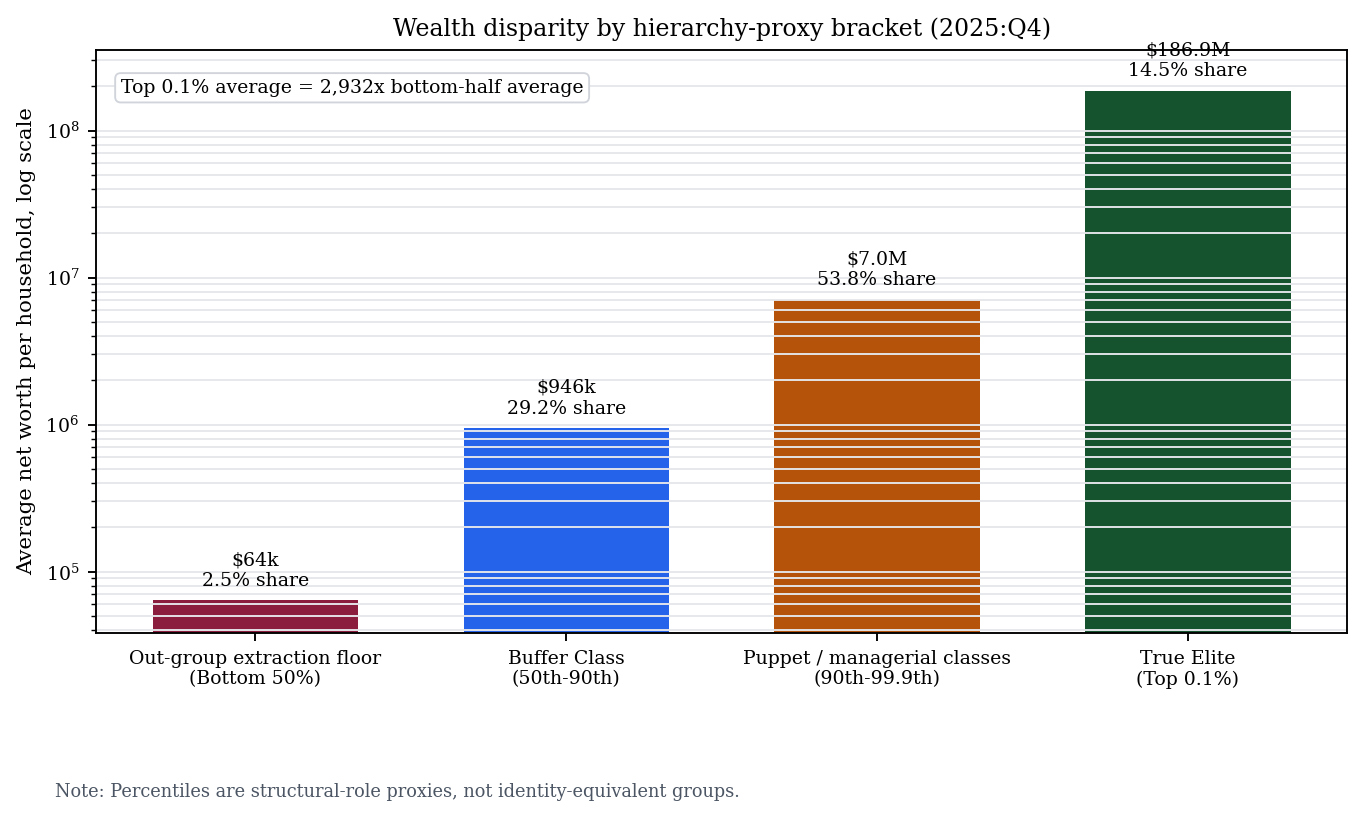
\includegraphics[width=\textwidth]{figures/eq10_hierarchy_wealth_brackets.png}
  \caption{\textbf{Wealth disparity by hierarchy-proxy bracket.} Federal Reserve DFA data for 2025:Q4 show the scale difference between the wealth brackets used as structural-role proxies in this case study: the Out-group extraction floor (bottom 50\%) averaged about \$64,000 in net worth per household and held 2.5\% of aggregate household net worth; the Buffer Class proxy (50th--90th percentiles) averaged about \$946,000 and held 29.2\%; the Puppet/managerial proxy (90th--99.9th percentiles) averaged about \$7.0 million and held 53.8\%; and the true Elite proxy (top 0.1\%) averaged about \$186.9 million while holding 14.5\%. The percentile brackets are distributional proxies for structural roles, not identity-equivalent groups.}
  \label{fig:hierarchy_wealth_brackets}
\end{figure}

\begin{figure}[htbp]
  \centering
  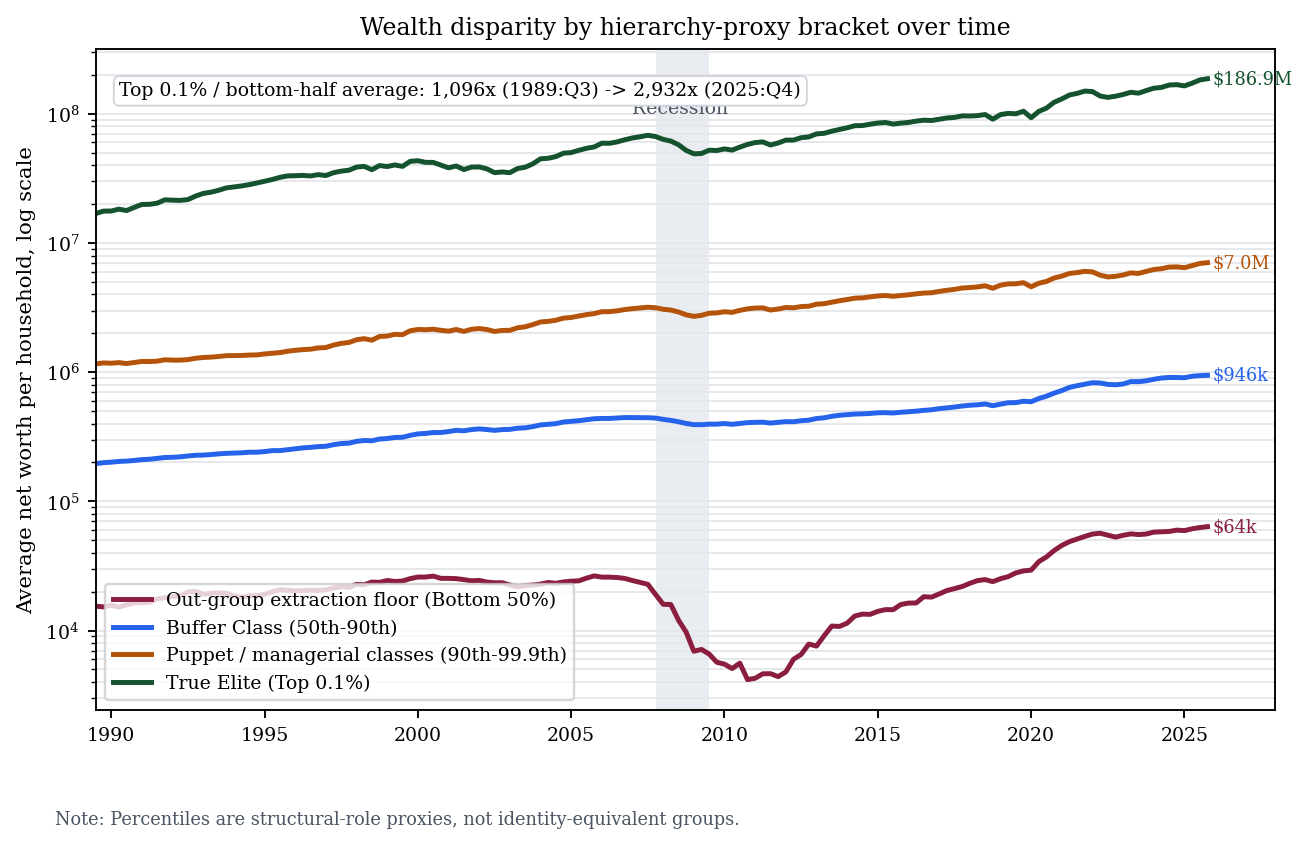
\includegraphics[width=\textwidth]{figures/eq10_hierarchy_wealth_brackets_over_time.png}
  \caption{\textbf{Wealth disparity by hierarchy-proxy bracket over time.} Federal Reserve DFA quarterly data show the same structural-role proxy brackets from 1989:Q3 through 2025:Q4. The average net worth of the true Elite proxy (top 0.1\%) was roughly 1,096 times the bottom-half proxy in 1989:Q3 and roughly 2,932 times the bottom-half proxy by 2025:Q4. The Great Recession appears as a visible floor collapse for the bottom 50\%, while the upper brackets experience interruption without long-run compression.}
  \label{fig:hierarchy_wealth_brackets_over_time}
\end{figure}

\begin{figure}[htbp]
  \centering
  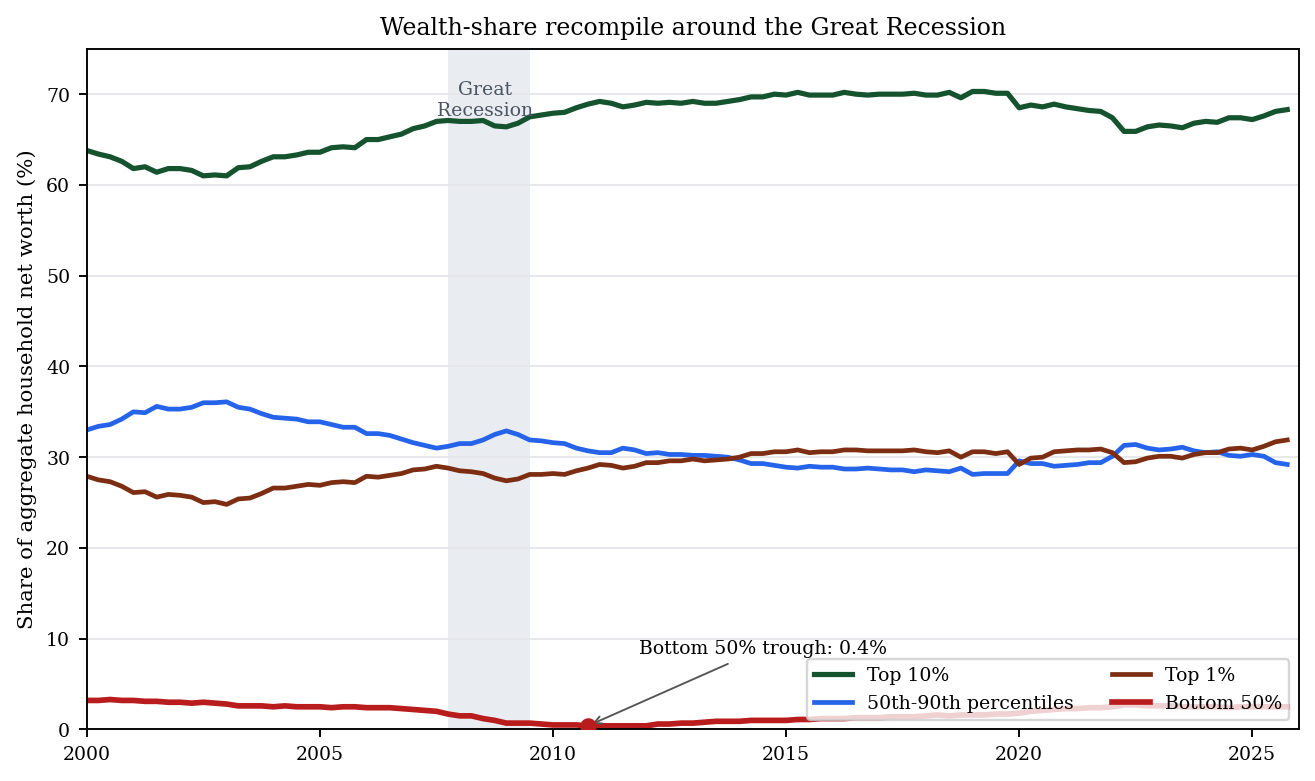
\includegraphics[width=\textwidth]{figures/eq10_great_recession_wealth_shares.png}
  \caption{\textbf{Wealth-share recompile around the Great Recession.} Federal Reserve DFA data show the bottom 50\%'s aggregate net-worth share falling from 1.7\% in 2007:Q4 to 0.4\% in 2011:Q4, while the top 10\% rose from 67.1\% to 68.8\% over the same window. By 2025:Q4, the top 1\% held 31.9\% of aggregate household net worth. The crash destroyed wealth at the base without producing a durable reduction in apex share, the empirical signature of $\Delta\max = 0$.}
  \label{fig:great_recession_wealth_shares}
\end{figure}

\paragraph{Numerical computation.}
The DFA wealth-share series gives the primary signature. In 2007:Q4, the top 10\% held 67.1\% of aggregate household net worth, the top 1\% held 28.8\%, the 50th--90th percentiles held 31.2\%, and the bottom 50\% held 1.7\%. By 2011:Q4, after the crash and the first phase of asset-market restoration, the bottom 50\% had fallen to 0.4\%, while the top 10\% had risen to 68.8\% and the top 1\% to 29.0\%. The lower half did not merely lose absolute dollars; it lost almost its entire already-small claim on national net worth. CBO independently reports that the 2007--2009 recession was the only significant decline in total family wealth from 1989 to 2022 and that the declines were steepest in the bottom half of the distribution \cite{cbo_family_wealth_2024}.

\begin{figure}[htbp]
  \centering
  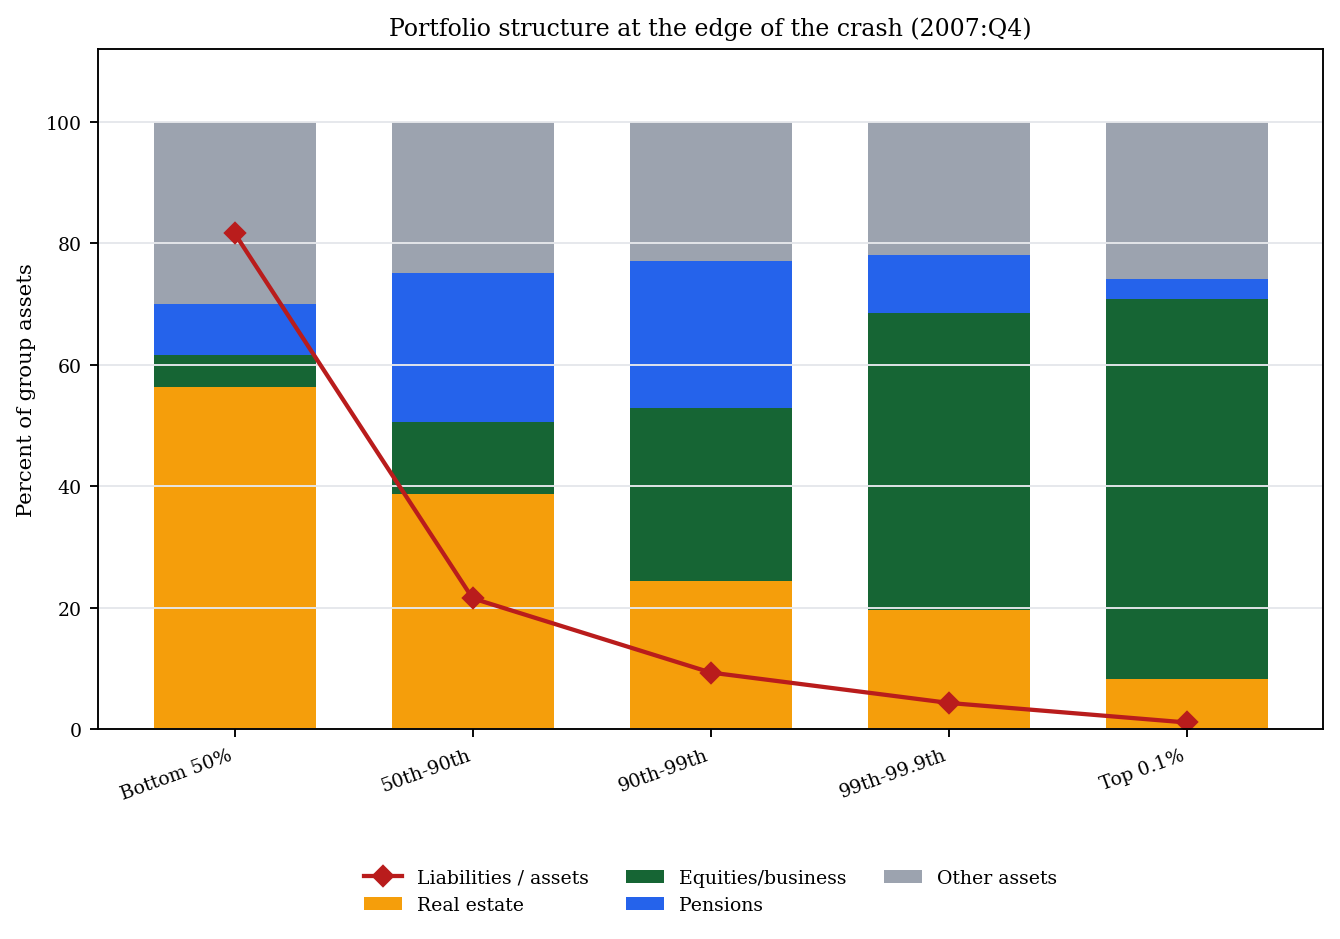
\includegraphics[width=\textwidth]{figures/eq10_great_recession_asset_composition.png}
  \caption{\textbf{Portfolio structure at the edge of the crash.} Federal Reserve DFA detailed levels for 2007:Q4 show why the crash was structurally asymmetric. For the bottom 50\%, real estate made up 56.3\% of assets and liabilities equaled 81.6\% of assets. For the top 0.1\%, real estate made up 8.3\% of assets, equity/business claims made up 62.5\%, and liabilities equaled only 1.2\% of assets. The same housing-price shock therefore struck a leveraged housing portfolio below while leaving the apex positioned for equity and asset-price recovery.}
  \label{fig:great_recession_asset_composition}
\end{figure}

The balance-sheet floor confirms the debt mechanism. In 2007:Q4, the bottom 50\% averaged approximately \$104,000 in assets and \$85,000 in liabilities per household, for an average net worth of roughly \$19,000. By 2010:Q4, average bottom-half net worth had fallen to about \$4,200, while liabilities still averaged nearly \$86,000. The collateral had been repriced downward; the debt claim remained.

\begin{figure}[htbp]
  \centering
  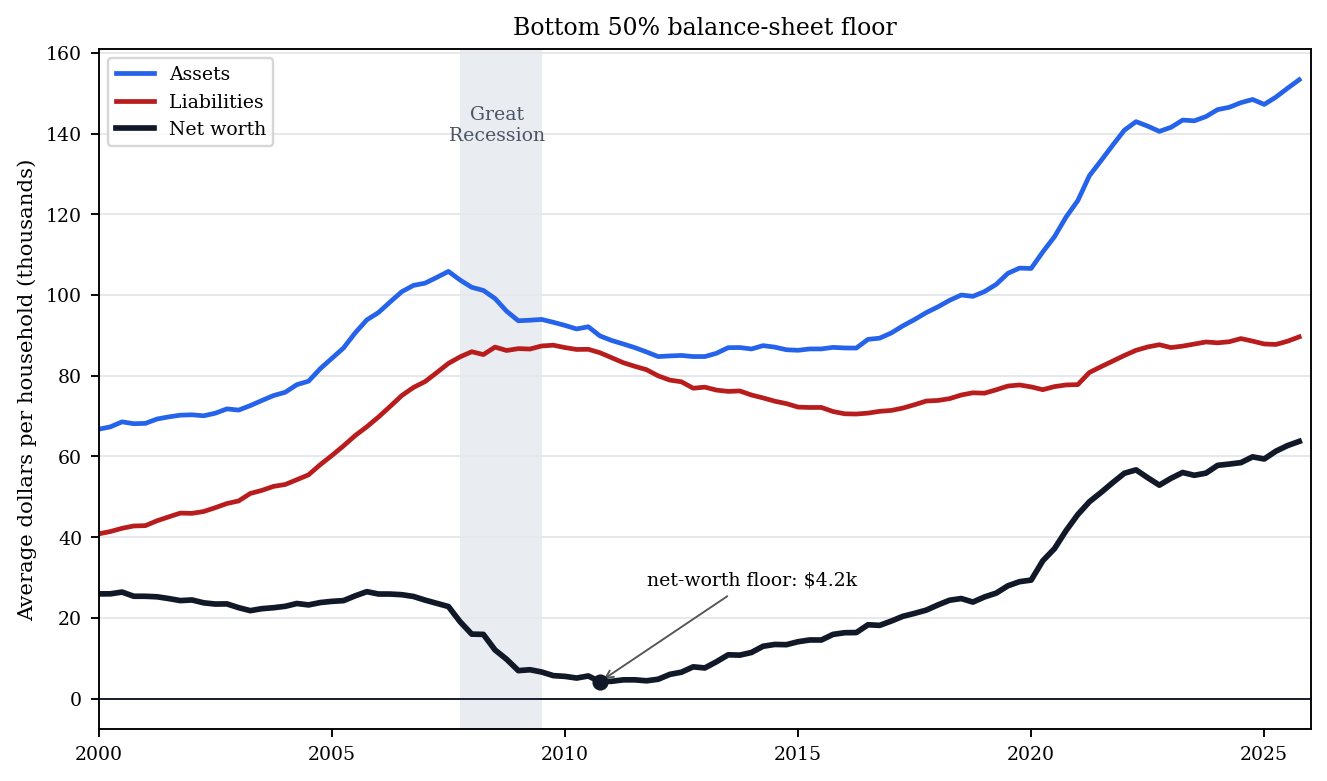
\includegraphics[width=\textwidth]{figures/eq10_great_recession_debt_floor.png}
  \caption{\textbf{Bottom-50 balance-sheet floor.} Federal Reserve DFA levels divided by household count show the household-scale version of temporal enclosure. Bottom-50 assets fell sharply through the crash while liabilities remained sticky, compressing average net worth from about \$19,000 in 2007:Q4 to a floor near \$4,200 in 2010:Q4. The future labor claim survived the asset collapse.}
  \label{fig:great_recession_debt_floor}
\end{figure}

\paragraph{Racialized loss channel.}
The crash was not only class-stratified; it was racially differentiated within the lower and middle tiers. Pew's SCF analysis reports that among middle-income households, Black median wealth fell 47\% from 2007 to 2013, Hispanic median wealth fell 55\%, and white median wealth fell 31\% \cite{pew_wealth_after_great_recession_2017}. Expressed in 2016 dollars, the implied 2007 middle-income medians were approximately \$63,000 for Black households, \$86,000 for Hispanic households, and \$191,000 for white households. By 2013, those medians had fallen to \$33,600, \$38,900, and \$131,900 respectively; by 2016, the white median had recovered to \$154,400, while Black and Hispanic middle-income medians remained at \$38,300 and \$46,000.

\begin{figure}[htbp]
  \centering
  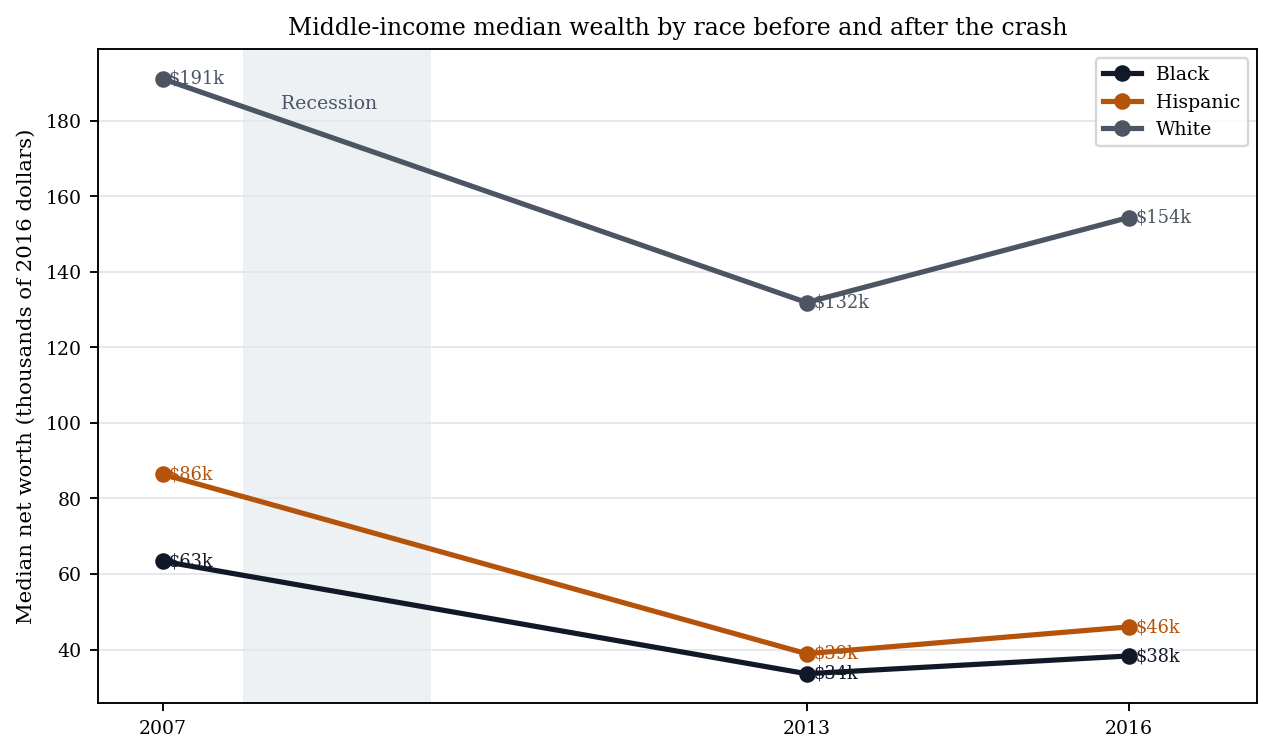
\includegraphics[width=\textwidth]{figures/eq10_great_recession_racial_wealth.png}
  \caption{\textbf{Middle-income median wealth by race before and after the crash.} Pew Research Center's SCF analysis shows that the housing-led crisis widened the racial wealth channel among middle-income households: Black and Hispanic households experienced larger percentage losses than white households from 2007 to 2013 and had not closed the gap by 2016. The mortgage market therefore transmitted the inherited geography of redlining into a nominally race-neutral balance-sheet shock.}
  \label{fig:great_recession_racial_wealth}
\end{figure}

Pfeffer, Danziger, and Schoeni provide the longitudinal confirmation: between 2007 and 2011, one fourth of American families with positive net worth lost at least 75\% of their wealth, more than half lost at least 25\%, and relative losses were disproportionately concentrated among lower-income, less-educated, and minority households \cite{pfeffer_danziger_schoeni_2013}. The system did not randomly distribute the crash. It followed the preexisting structure of exposure: housing-heavy portfolios, thin liquidity, high leverage, and racialized credit channels.

\paragraph{Comparison to prediction.}
The framework predicts that a crisis under sub-$\tau$ conditions will be absorbed as an interface recompile rather than a kernel loss. The Great Recession matches that prediction. The base and lower-middle tiers absorbed the balance-sheet destruction; the debt claims against them persisted; asset-market intervention restored the financial instruments disproportionately held by the top decile; and the apex share did not undergo durable reduction. In set-theoretic terms, the crisis degraded $O_{\text{racialized}}$ first and then proved that the lower strata of $I_{\text{buffer}}$ could be harvested through the same balance-sheet machinery. The material wage of homeownership became an extraction surface.

\paragraph{Falsification criteria.}
This case would falsify the Great Recession recompile claim if the 2007--2012 evidence showed a durable reduction in top-tier wealth share, no disproportionate housing-wealth loss among lower-wealth households, no racialized foreclosure or wealth-loss gradient, and no post-crisis asset recovery concentrated among equity- and real-estate-owning tiers. The observed data move in the opposite direction on each dimension.

\paragraph{Confidence tier.}
\textbf{Tier~1.} Federal Reserve DFA public data, CBO family-wealth distribution data, Pew SCF analysis, and peer-reviewed PSID/SCF longitudinal evidence all align on the direction of the case: wealth destruction was concentrated below the apex, racialized within the middle and lower tiers, and followed by restoration of asset-owning tiers rather than durable reduction in $E$'s extraction share.

\section{The Collapse: Cannibalizing the In-Group (Present)\protect\footnote{The term \textit{cannibalizing} here describes the structural consumption of the In-group's wealth and autonomy. This metaphorical use of consumption must be explicitly distinguished from the literal and libidinal consumption of the Out-group documented in Section~\ref{subsec:libidinal_extraction}, which was not a metaphor but a historical, material practice \cite{woodard_delectable}.}}
This brings us to the final, inevitable stage of the algorithm. An extraction system requires \textbf{Infinite Growth}. Once the Out-group ($O$) has been fully harvested---stripped of wealth, voting rights, and labor \cite{coates}---the Elite ($E$) must find new sources of extraction to maintain their accumulation.

A definitional clarification before the case evidence: within the framework, ``terminal phase'' does not mean imminent system collapse. Venice's \textit{Serrata} operated in its terminal phase---oligarchic cannibalization of the commercial base---for nearly five centuries before the Republic's formal dissolution under Napoleon in 1797. Rome's latifundia terminal phase ran from roughly the Gracchan period (133~BC) through the fall of the Western Empire in 476~AD---over six hundred years. Extraction systems are not brittle; they adapt. ``Terminal'' is a \textit{set-theoretic} designation: the extraction boundary has reached its logical endpoint $O_{\text{final}} = \text{Everyone} \setminus E$ (Equation~\ref{eq:10.12-o-final-construction}), meaning the algorithm has exhausted its original partitioning strategy and begun consuming its own intermediate enforcement tiers. The system does not terminate when it enters this phase; it deploys new proxy variables---$P_{\text{toxin}}$, $P_{\text{spatial}}$, universal latent criminality---to manage the extraction of a population that was previously its enforcement coalition. The terminal phase is therefore not a \textit{prediction} of collapse; it is a description of the current operating mode, identifiable by the simultaneous deployment of extraction tools against $I_{\text{buffer}}$ that were previously reserved for $O_{\text{racialized}}$. What ends in the terminal phase is not the system but the buffer class's conditional immunity.

The pattern has historical precedents that institutional economics identifies but does not explain. Acemoglu and Robinson document two canonical cases of extraction-kernel self-consumption \cite{acemoglu_robinson}: Venice's \textit{Serrata} of 1297, in which the ruling merchant oligarchy closed the Great Council to new members, institutionalizing their monopoly, then gradually extracted so much from the broader commercial class that Venetian trade declined and the oligarchs ultimately cannibalized the very commercial base that had generated their wealth; and Rome's latifundia expansion, in which the agrarian Elite's seizure of land worked by slave labor drove the free peasantry off their holdings and into dependency, eliminating the smallholder class that had been the backbone of the legions---in effect consuming the military-human capital that had made Roman expansion possible. In both cases, the extraction kernel turned on its own In-group when the Out-group's capacity was fully depleted. The framework adds the variable that explains the mechanism AJR cannot: the psychological wage ($\psi$) that prevented the Buffer Class from forming a defensive coalition with $O_{\text{racialized}}$ while both were being extracted also prevented it from forming a defensive coalition with $O_{\text{racialized}}$ as the cannibalization began. By the time the wages of whiteness were bankrupt, the institutional means of cross-class coordination had been systematically dismantled.

The Great Recession supplied the domestic proof of this transition. The racialized foreclosure wave first struck $O_{\text{racialized}}$ through the accumulated geography of redlining and predatory lending, but the same balance-sheet mechanism then consumed the lower strata of $I_{\text{buffer}}$: home equity vanished, debt claims survived, and the recovery restored asset values primarily for those already positioned in equities, bonds, and institutional real estate. The crisis therefore marks the inflection at which the material wage of homeownership stopped functioning as a durable buffer and became an extraction surface.

\begin{figure}[htbp]
\centering
\begin{tikzpicture}
\begin{axis}[
    width=0.95\textwidth,
    height=7.5cm,
    xmin=0, xmax=10,
    ymin=0, ymax=1.1,
    xtick={1, 3, 5, 7, 9},
    xticklabels={Pre-Civil War, Reconstruction, Jim Crow, Civil Rights, Present},
    xlabel={Historical Phase},
    ylabel={Relative Extraction Intensity},
    xlabel style={font=\small},
    ylabel style={font=\small},
    title={\textbf{The Cannibalization Phase Transition}},
    title style={font=\bfseries\small},
    legend style={at={(0.03,0.97)}, anchor=north west, font=\scriptsize, fill=white, fill opacity=0.9, draw=gray},
    grid=major,
    grid style={gray!20},
]

% Extraction from O_racialized
\addplot[very thick, red!80!black, smooth] coordinates {
    (0,0.4) (1,0.8) (3,0.9) (5,0.95) (7,0.85) (9,0.7) (10,0.6)
};
\addlegendentry{Extraction from $O_{\text{racialized}}$}

% Extraction from I_buffer
\addplot[very thick, orange, dashed, smooth] coordinates {
    (0,0.1) (1,0.1) (3,0.15) (5,0.2) (7,0.4) (9,0.85) (10,1.0)
};
\addlegendentry{Extraction from $I_{\text{buffer}}$}

% Shading current phase
\fill[orange!10, opacity=0.5] (axis cs:7.5,0) rectangle (axis cs:10,1.1);
\node[anchor=north, font=\tiny\bfseries, text=orange!70!black, align=center] at (axis cs:8.75,1.05) {Current Phase:\\$I_{\text{buffer}}$ being consumed};

% Cannibalization Inflection
\draw[thick, black!60, dashed] (axis cs:7.8,0) -- (axis cs:7.8,1.1);
\node[rotate=90, anchor=south, font=\tiny\bfseries, text=black!60] at (axis cs:7.8,0.5) {Cannibalization Inflection};

% Callouts
\node[circle, fill=red!80!black, inner sep=1pt, label={above right:\tiny Venice Serrata (1297)}] at (axis cs:0.5,0.45) {};
\node[circle, fill=orange, inner sep=1pt, label={below:\tiny Ruby Ridge/Waco}] at (axis cs:8.2,0.6) {};
\node[circle, fill=orange, inner sep=1pt, label={right:\tiny Opioid Crisis}] at (axis cs:9.2,0.9) {};

\end{axis}
\end{tikzpicture}
\caption{\textbf{The Cannibalization Phase Transition.} As the capacity for extraction from the racialized Out-group ($O_{\text{racialized}}$) plateaus and begins to decline due to systemic depletion, the extraction kernel must turn inward to maintain infinite growth. The dashed orange line represents the escalating extraction from the Buffer Class ($I_{\text{buffer}}$). The Cannibalization Inflection marks the point where the tools of subjugation developed for the Out-group are fully redeployed against the In-group.}
\label{fig:cannibalization_phase}
\end{figure}

The system has now turned inward. The tools developed to oppress the Out-group are being deployed against the In-group:
\begin{itemize}
    \item \textbf{The Opioid Crisis:} The criminalization of white addiction mirrors the crack epidemic.
    \item \textbf{Militarized Policing:} SWAT tactics invented for the "Ghetto" are now used in rural towns.
    \item \textbf{Surveillance:} The loss of privacy tested on the poor is now applied to the middle class.
\end{itemize}

The expansion of $O$ is facilitated by a structural development that legal scholar Harvey Silverglate identifies: the average American now unknowingly commits approximately \textbf{three federal felonies per day} \cite{silverglate}. The proliferation of vague, overlapping, and over-broad criminal statutes---combined with prosecutorial discretion in charging---means that the proxy variable $P$ has become \textit{omnipresent}. Nearly every citizen is technically criminal; what determines who enters the carceral system is not the commission of crime but the \textit{selection} of targets. This transforms the system's primary mechanism from demographic targeting to \textbf{selective enforcement}: the Elite no longer needs to define the Out-group explicitly, because the criminalization kernel ($\text{If } \text{Status}(x) = \text{Criminal}(C) \rightarrow \text{Status}(x) \in S$) can now reach \textit{anyone}. ``Broken windows'' policing \cite{wilson} and its progeny provide the discretionary framework---the theoretical justification for intensive policing of minor infractions---while the empirical evidence shows that such policing is deployed overwhelmingly in communities already marked by the compounding chain of Section~4.5 \cite{harcourt}. The system has thus achieved what might be called \textbf{universal latent criminality}: the entire population exists in a state of potential subjugation, with actual subjugation determined by $E$'s extraction needs.

\section{The Recursive Extraction Engine: Biological Degradation as Control}

To fully comprehend the Elite subset’s ($E$) control matrix, the analysis must expand beyond legal and labor extraction to include the deliberate manipulation of the population's biological autonomy. The contemporary Medical-Industrial Complex (MIC) and the subsidized agricultural sector do not operate independently; they function as a unified, recursive extraction algorithm.

Within this framework, the system is designed to transition the population from a state of symmetrical biological autonomy ($O_{\text{full\_capacity}}$) into a state of chronic, manageable illness ($O_{\text{degraded}}$). A biologically compromised population serves a dual function for the Elite: it generates infinite, recurring revenue, and it physiologically neutralizes the capacity for class resistance \cite{washington}.

\subsection{Phase 1: The Toxin Variable (\texorpdfstring{$P_{\text{toxin}}$}{P\_toxin}) and the "Affordability Trap"}

The extraction loop begins with the engineered degradation of the food supply. The system utilizes seemingly neutral economic policies ($P$)—specifically agricultural subsidies and a reversed regulatory framework (such as the FDA's "Generally Recognized as Safe" or GRAS loophole, which allows manufacturers to self-regulate)—to flood the market with high-fructose corn syrup, refined grains, and chemical additives. Currently, nearly 70\% of packaged foods in the U.S. are classified as ultra-processed, supplying more than half of adults' daily calories.

This is not an accident of the free market; it is a meticulously engineered "Affordability Trap" designed to aggressively target the Out-group ($O$) and the lower-tier Buffer Class ($I \setminus E$). A 2026 comprehensive audit by Harvard Law School’s Food Law and Policy Clinic mathematically proved that price strictly dictates a population's exposure to toxicity.
The study revealed a stark biological matrix:
\begin{itemize}
    \item \textbf{The Additive Multiplier}: The lowest-priced food products contain, on average, 2.6 times more additives than the most expensive options (averaging 6.6 additives per item versus 2.7).
    \item \textbf{High-Risk Concentration}: In staple categories, the disparity accelerates. The cheapest store-bought breads contain nearly 4 times more additives, and the cheapest frozen pizzas contain an average of 12 additives per product (compared to 4.4 in the highest tier). Most critically, the cheapest products contain over 3 times more high-risk, health-compromising additives.
    \item \textbf{The Caloric Payload}: Lower-priced foods are engineered to be chemically addictive and physiologically destructive, containing 21\% more sugar and 10\% more sodium than their higher-priced counterparts.
\end{itemize}
To maintain baseline biological autonomy—meaning, to consume products free of high-risk additives—a consumer must pay an average price premium of 63\%.

Within the Predatory Min-Max Function, this 63\% premium functions as a biological poll tax. The Elite class ($E$) sets the financial threshold for physical health intentionally out of reach for the racialized Out-group ($O_{\text{racialized}}$), forcing them to consume the very toxins that will push them into the $O_{\text{degraded}}$ state. By making optimal nutrition artificially expensive and toxic food artificially cheap, the system mathematically guarantees the mass onset of chronic conditions such as obesity, hypertension, and Type 2 diabetes. The Out-group is not "choosing" a poor diet; they are being economically confined to a designated toxicity zone.

\section{The Cannibalization of the Buffer Class and the Endpoint of the Algorithm}

Section~6.12 established the structural transition: as extraction from $O_{\text{racialized}}$ saturates, the kernel expands toward $O_{\text{final}}=\text{Everyone}\setminus E$. This section executes that transition at case level. The "White Working Class" was never a partner to the Elite; they were a temporary reserve. A fundamental theorem of the Predatory Min-Max Function is that the Elite ($E$) has no permanent loyalty to the Buffer Class ($I_{\text{buffer}}$). As Elite demand for control intensifies, conditional privileges are revoked and the extraction boundary expands from $O_{\text{racialized}}$ toward $O_{\text{final}}$.

The ultimate, devastating proof of this terminal phase is the 2026 killing of Alex Perdi by Immigration and Customs Enforcement (ICE) agents. Demographically, as a cisgender white man, Perdi represented the historical core of the protected Buffer Class. Under the ideological justification (Component 3) of the Second Amendment, his decision to arm himself in confrontation with law enforcement should theoretically have been shielded by the same ``anti-tyranny'' constitutional interpretations routinely afforded to the In-group. (The reclassification operator $\mathcal{R}$ that executed against Perdi in 2026 is not a post-2020 innovation; its 1992--94 historical instantiations at Ruby Ridge and Waco are documented in $\S$\ref{sec:ruby_ridge_waco}.)

\subsection{Disarmament and Execution: The Algorithm Unmasked}
However, the reality of the encounter proved that the system's operational code has shifted. During the confrontation, Perdi was successfully disarmed. At the exact moment he lost his lethal autonomy, he ceased to be a member of the protected class. He was no longer treated as a citizen possessing constitutional rights; the state enforcement algorithm immediately reclassified him as a neutralized biological asset and executed him.

This event mathematically shatters the core illusion of the American operating system. It demonstrates that the state's enforcement apparatus—originally designed as slave patrols to violently manage the racialized Out-group—has now been fully authorized to deploy lethal extraction against anyone outside of the true Elite ($E$), regardless of their demographic status.

The execution of a disarmed white citizen by federal agents proves that the "wages of whiteness" are effectively bankrupt. The Second Amendment does not protect the Buffer Class from state violence; it merely serves as a temporary pacifier until the state decides to revoke it. The system has reached its most optimized, terrifying state: a pure binary where absolute immunity is reserved exclusively for the Elite ($E$), and every other citizen is mathematically confined to the Out-group, waiting to be harvested.

The definition of the Out-group has returned to its 1676 state:

\begin{equation}\label{eq:10.12-o-final-construction}
O_{\text{final}} = \text{Everyone} \setminus E
\end{equation}

The dynamic mechanism by which individual citizens cross this boundary---the reclassification operator $\mathcal{R}(x_i)$---is formalized in $\S$\ref{sec:ruby_ridge_waco} (see equation~\eqref{eq:10.13-reclassification-operator}) and registered in the Canonical Symbol Registry (Appendix~\ref{sec:equation_registry}). Equation~\eqref{eq:10.12-o-final-construction} gives the static endpoint of the expansion; $\mathcal{R}(x_i)$ gives the conditional function that assigns each individual to either side of the partition at runtime.

\subsection*{Case Study: Mass Incarceration and the Expanding Out-Group}
\label{cs:mass_incarceration}

\paragraph{Setup.}
Equation~\ref{eq:10.12-o-final-construction} predicts that the extraction system's terminal state is $O_{\text{final}} = \text{Everyone} \setminus E$ --- the out-group expands until it contains everyone except the Elite. Mass incarceration demographics provide the most direct measurable test of this prediction. If $O_{\text{final}}$ is the predicted terminal state, then: (1) Black Americans (the historically designated $O_{\text{racialized}}$) should sustain the highest per-capita incarceration rates throughout; (2) the system should expand its reach to absorb progressively larger fractions of $I_{\text{buffer}}$ (White and Hispanic populations) over time; and (3) $E$ should maintain effectively zero incarceration rate at all periods, confirming the partition $O_{\text{final}} \cap E = \emptyset$.

\paragraph{Data sources.}
Per-race incarceration data are drawn from the Bureau of Justice Statistics (BJS) National Prisoner Statistics program \cite{bjs_incarceration_race} covering state and federal prisons, supplemented by local jail population estimates. Racial disparity ratios are cross-validated against The Sentencing Project's annual state-by-state reports \cite{sentencing_project} and Alexander (2010) \cite{alexander}. Population denominators are from Census Bureau estimates. Data span 1980--2024, capturing the full mass incarceration arc. Curated data are archived at \texttt{Paper/data/eq63\_mass\_incarceration.csv}; computational results are reproducible via \texttt{Paper/scripts/eq63\_mass\_incarceration.ipynb}.

\paragraph{Operationalization.}
The set-theoretic prediction is operationalized as follows: $O_{\text{final}}$ = total incarcerated population (everyone inside the carceral system); $E$ = top wealth percentile (empirically, near-zero incarceration rate at all time points); the expansion from $O_{\text{racialized}}$ toward $O_{\text{final}}$ = the growth of White and Hispanic incarceration rates relative to total population after 1994 (the 1994 Crime Bill as the key policy shock). The Black-to-White incarceration ratio tracks whether racial targeting within $O_{\text{final}}$ is maintained even as the out-group expands.

\paragraph{Numerical computation.}
The notebook yields the following key figures. Total incarcerated: $\approx$503,586 (1980) $\rightarrow$ $\approx$2,307,504 peak (2008), a 3.6$\times$ increase. Black-to-White per-capita incarceration ratio: range 3.92--6.11 across 1980--2024, mean 4.61; the ratio has never fallen below 3.9 in any year of the dataset, confirming persistent racial targeting. Post-1994 Crime Bill expansion ($O_{\text{final}}$ growth into $I_{\text{buffer}}$): White incarceration grew $\approx$15\% from 1994 to 2000; Hispanic incarceration grew $\approx$100\% over the same period. Elite incarceration rate: effectively 0 per 100k at all time points, consistent with $E \cap O_{\text{final}} = \emptyset$.

\begin{figure}[htbp]
  \centering
  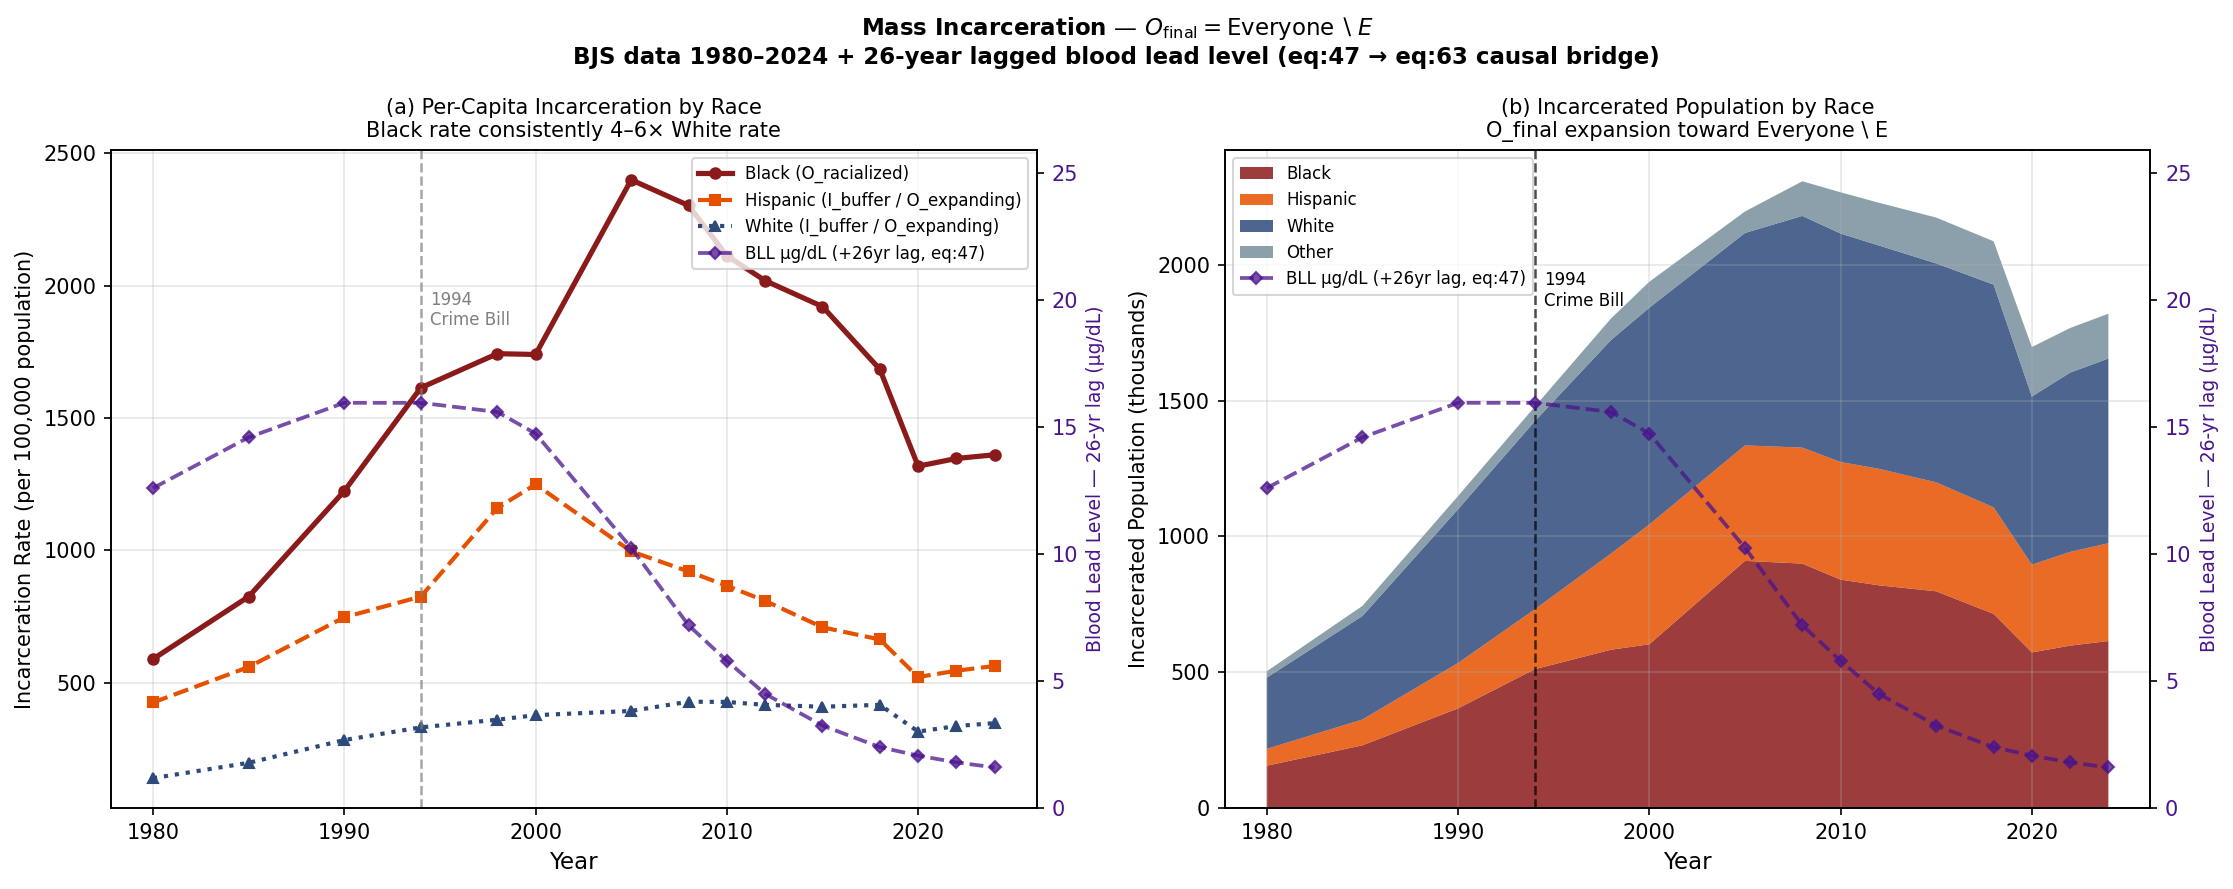
\includegraphics[width=\textwidth]{figures/eq63_mass_incarceration.png}
  \caption{Mass incarceration demographics, 1980--2024 (BJS data), with 26-year lagged blood lead level (BLL, purple dashed, right axis) overlaid on both panels. Left: per-capita incarceration rates by race --- Black rate consistently 4--6$\times$ White rate. Right: stacked area chart of incarcerated population by race. Two lagged BLL series are overlaid. The blue line (+20 years, Reyes 2007) reflects the crime-rate lag: peak BLL from $\approx$1972 shifts forward to $\approx$1992, coinciding with the documented crime-rate peak of 1991--93. The purple line (+26 years, two-stage) decomposes into the same 20-year behavior-onset lag plus an additional $\approx$6-year sentence-accumulation effect (Mauer \& King, 2007): as the crime-affected cohort cycles through arraignment, sentencing, and multi-year mandatory minimums, the incarceration \textit{count} peaks later than the crime \textit{rate}. The purple line's peak ($\approx$1998) aligns with the incarceration-count surge; its post-1986-BLL decline aligns with the post-2012 plateau. The visible $\approx$6-year gap between the two lines is the quantitative signature of the sentence-accumulation effect introduced by the 1994 Crime Bill's mandatory minimums. This overlay bridges eq.~\ref{eq:9.1-lead-crime-compounding}--\ref{eq:9.10-highway-lead-spatial-concentration} and eq.~\ref{eq:10.12-o-final-construction}: the spatially targeted neurotoxin exposure identified in Chapter~9 is a measurable leading indicator of the carceral expansion documented here. The 1994 Crime Bill marker shows the legislative shock that converted a lead-driven behavioral vulnerability into a policy-amplified $O_{\text{final}}$ expansion.}
  \label{fig:eq63_mass_incarceration}
\end{figure}

\paragraph{Comparison to prediction.}
Equation~\ref{eq:10.12-o-final-construction} predicts expansion beyond $O_{\text{racialized}}$ as the system optimizes toward its terminal state. The data confirm this at every level: while Black Americans remain the most disproportionately targeted group (4--6$\times$ White per-capita rate throughout), the carceral system progressively absorbed larger fractions of $I_{\text{buffer}}$ --- particularly after the 1994 Crime Bill's mandatory minimums and ``three strikes'' provisions. The 3.6$\times$ total incarceration growth (1980--peak) while crime declined (peak 1993, declining through 2010) confirms that the expansion is driven by policy architecture ($P_{\text{puppet}}$ legislative agenda), not by behavioral change in the population. The Elite partition ($E \approx 0$ incarceration rate) is empirically stable across the full 44-year window.

\paragraph{Falsification criteria.}
This equation would be falsified if modern mass-incarceration demographics showed the carceral system contracting to target only $O_{\text{racialized}}$ rather than expanding toward $\text{Everyone} \setminus E$. Specifically: if White and Hispanic incarceration rates had declined after 1994 while Black rates grew, the $O_{\text{final}}$ expansion prediction would be refuted. The data show the opposite: all non-elite groups experienced expansion after 1994, with the 1994 Crime Bill serving as the documented policy trigger for $I_{\text{buffer}}$ absorption into the carceral system.

\paragraph{Confidence tier.}
\textbf{Tier~1.} Forty-four-year continuous BJS dataset; racial disparity ratios independently verified by The Sentencing Project, the ACLU, and peer-reviewed criminology literature; the crime-decline vs.\ incarceration-growth divergence (post-1993) is a documented empirical fact replicated across all major crime and incarceration databases.

\begin{figure}[h]
    \centering
    \begin{tikzpicture}[scale=0.88, every node/.style={font=\small}]

    % --- Phase 1: 1676 (United labor) ---
    \begin{scope}[shift={(0,0)}]
        \node[font=\footnotesize\bfseries, anchor=south] at (1.5,2.85) {1676: Unity};
        % Elite box
        \draw[thick, green!60!black, fill=green!40] (0.8,1.8) rectangle (2.2,2.6);
        \node[green!60!black, font=\scriptsize] at (1.5,2.2) {$E$};
        % United labor
        \draw[thick, purple!70, fill=purple!20] (0,0) rectangle (3,1.5);
        \node[purple!70, font=\scriptsize, align=center] at (1.5,0.75) {$L_{white} \cup L_{black}$\\(United Labor)};
        % Threat arrow
        \draw[->, very thick, red!70] (1.5,1.5) -- (1.5,1.8);
        \node[red!70, font=\tiny, rotate=90] at (0.3,1.65) {Threat};
    \end{scope}

    % Arrow
    \draw[->, very thick, gray] (3.3,1.2) -- (4.0,1.2);

    % --- Phase 2: 1705 (Partition) ---
    \begin{scope}[shift={(4.3,0)}]
        \node[font=\footnotesize\bfseries, anchor=south] at (1.5,2.85) {1705: Partition};
        % Elite box
        \draw[thick, green!60!black, fill=green!40] (0.8,1.8) rectangle (2.2,2.6);
        \node[green!60!black, font=\scriptsize] at (1.5,2.2) {$E$};
        % Buffer class (white)
        \draw[thick, blue!70, fill=blue!15] (0,0.8) rectangle (3,1.5);
        \node[blue!70, font=\scriptsize] at (1.5,1.15) {$I_{\text{buffer}}$};
        % Extraction zone (black)
        \draw[thick, red!80, fill=red!30] (0,0) rectangle (3,0.65);
        \node[red!80, font=\scriptsize] at (1.5,0.32) {$O_{\text{racialized}}$ (Enslaved)};
        % Shield arrow
        \draw[->, thick, blue!70] (1.5,1.5) -- (1.5,1.8);
        \node[blue!70, font=\tiny, rotate=90] at (0.3,1.65) {Shield};
    \end{scope}

    % Arrow
    \draw[->, very thick, gray] (7.6,1.2) -- (8.3,1.2);

    % --- Phase 3: 1865--1968 (Expansion) ---
    \begin{scope}[shift={(8.6,0)}]
        \node[font=\footnotesize\bfseries, anchor=south] at (1.5,2.85) {1865--1968};
        % Elite box
        \draw[thick, green!60!black, fill=green!40] (0.8,1.8) rectangle (2.2,2.6);
        \node[green!60!black, font=\scriptsize] at (1.5,2.2) {$E$};
        % Buffer class (shrinking)
        \draw[thick, blue!70, fill=blue!15] (0,1.1) rectangle (3,1.5);
        \node[blue!70, font=\scriptsize] at (1.5,1.3) {Buffer (shrinking)};
        % Expanded extraction zone
        \draw[thick, red!80, fill=red!30] (0,0) rectangle (3,0.95);
        \node[red!80, font=\scriptsize, align=center] at (1.5,0.48) {$O_{\text{racialized}}$ + Criminalized\\+ Drug-Targeted};
    \end{scope}

    % Arrow
    \draw[->, very thick, gray] (11.9,1.2) -- (12.6,1.2);

    % --- Phase 4: Present (Cannibalization) ---
    \begin{scope}[shift={(12.9,0)}]
        \node[font=\footnotesize\bfseries, anchor=south] at (1.5,2.85) {Present};
        % Elite box
        \draw[thick, green!60!black, fill=green!40] (0.8,1.8) rectangle (2.2,2.6);
        \node[green!60!black, font=\scriptsize] at (1.5,2.2) {$E$};
        % Extraction zone consuming nearly everything
        \draw[thick, red!80, fill=red!30] (0,0) rectangle (3,1.5);
        \node[red!80, font=\scriptsize, align=center] at (1.5,0.75) {$O_{\text{final}}$\\$= \text{Everyone} \setminus E$};
        % Cannibalization arrow
        \draw[->, very thick, red!80, dashed] (1.5,1.5) -- (1.5,1.8);
        \node[red!80, font=\tiny, rotate=90] at (0.15,1.65) {Threat};
    \end{scope}

    % Bottom annotation
    \draw[->, very thick, red!60] (0,-0.5) -- (15.9,-0.5);
    \node[red!60, font=\footnotesize, anchor=west] at (4.5,-0.9) {Extraction zone expands $\longrightarrow$ Buffer consumed};

    \end{tikzpicture}
    \caption{\textbf{The Recursive Expansion of the Extraction Zone (1676--Present).} This diagram illustrates the ``Min-Max'' algorithm in motion. Following the threat of unity in 1676, the Elite created a racial partition to separate the labor force. However, as the extraction system requires infinite growth, the Out-group boundary expands from $O_{\text{racialized}}$ toward $O_{\text{final}}$---first through chattel slavery, then through criminalization during the War on Drugs, and finally through cannibalization of $I_{\text{buffer}}$ in the modern phase. The Buffer Class was never a permanent partner to the Elite, but a temporary reserve of capital.}
    \label{fig:extraction_zone}
\end{figure}

\section{The First Cannibalization Signal: Ruby Ridge, Waco, and the Reclassification of the Buffer Class (1992--1994)}
\label{sec:ruby_ridge_waco}

The preceding sections established the terminal trajectory analytically and closed it with the 2026 Perdi execution as a contemporary proof. The natural objection is temporal: a single 2026 incident cannot sustain a claim of \textit{structural} cannibalization. The framework answers that objection by locating the first empirically anchored, live-action instantiations of the reclassification machinery in the early 1990s. The federal sieges at Ruby Ridge, Idaho (August 1992), and the Mount Carmel Center outside Waco, Texas (February--April 1993), are not episodes of government overreach to be explained away as tactical failures. They are the moment when elements of $I_{\text{buffer}}$---rural, overwhelmingly white, economically peripheral, and armed---were stripped of $\psi_s$ protections and processed by $F_{\text{enforce}}$ under rules of engagement previously reserved for $O_{\text{racialized}}$. What the previous section described as metaphorical ``cannibalization'' (see the footnote opening $\S$\ref{sec:full_reveal} distinguishing the intra-class metaphor from \texttt{libidinal\_extraction.exe}) executed in kinetic mode as early as 1992. The thirty-four-year gap between Ruby Ridge and the 2026 Perdi killing is not evidence of discontinuity; it is evidence that the reclassification operator has been a continuously available kernel subroutine for over a generation.

\subsection{The Pretext Subroutine: NFA Violations as Legal Proxy}
\label{subsec:nfa_pretext}

The extraction algorithm does not initiate kinetic violence against $I_{\text{buffer}}$ through explicit ideological targeting; doing so would prematurely expose the system's conditional hostility to its own defenders. Instead, the system relies on bureaucratic and legal proxy variables, and the cleanest such variable in both sieges is the National Firearms Act (NFA) of 1934. The NFA analysis in $\S$\ref{sec:statute_evolution_usc}ff. documented that the NFA was designed as an economic filter---a prohibition-disguised-as-tax that transforms the kinetic guarantee into a luxury commodity. The same statute, evaluated on a different demographic input, functioned as the pretext subroutine that authorized the deployment of lethal federal force against the Buffer Class in 1992--93. The substance-invariance argument developed at $\S$\ref{sec:full_reveal} applies directly here: change the target demographic, keep the statute, and the algorithm produces the identical output.

The entrapment of Randy Weaver illustrates the generative step. In October 1989, a Bureau of Alcohol, Tobacco, and Firearms (ATF) confidential informant, Kenneth Fadeley, induced Weaver to sell two shotguns whose barrels were cut one-quarter inch below the federal eighteen-inch NFA threshold \cite{dojruby1994}. When Weaver refused subsequent attempts to recruit him as an informant inside the Aryan Nations network, the ATF indicted him on federal firearms charges in June 1990. A federal probation officer then sent Weaver a letter misstating his trial date---March 20 rather than February 20, 1991---producing the bench warrant under which the United States Marshals Service subsequently conducted the August 1992 surveillance that precipitated the firefight \cite{dojruby1994, oprruby2001}. The state manufactured a minor, victimless NFA discrepancy through active entrapment, converted it via a bureaucratic clerical error into ``failure to appear'' fugitive status, and thereby generated the pretext required to deploy a militarized apprehension operation against a rural cabin.

A structurally identical sequence initiated the Waco siege. The ATF's February 1993 investigation of the Branch Davidians at the Mount Carmel Center cited the sect's stockpile of 136 firearms, more than 200{,}000 rounds of ammunition, over 700 magazines, inert M31 practice rifle grenades, and AR-15 lower receivers---a catalogue the Treasury Department's post-siege review codified \cite{treasury1993waco, danforth2000}. Most of the hardware had been lawfully acquired through David Koresh's retail firearms business; the ATF's legal theory aggregated otherwise legal purchases into a claim of coordinated NFA violation. The agency bypassed available non-violent apprehension pathways---Koresh left the compound routinely and was known to local law enforcement---in favor of a dynamic entry involving more than seventy heavily armed agents. The framework diagnostic is immediate: the ATF operated exactly as the paper's $F_{\text{enforce}}$ model predicts, seeking hardware parity that threatens $L_E \gg L_O$ \cite{treasury1993waco}. The NFA was not deployed as a public-safety instrument; it was deployed as a jurisdictional skeleton key authorizing the kinetic neutralization of populations that had functionally seceded from Elite economic and ideological control.

\begin{table}[htbp]
\centering
\small
\caption{Ruby Ridge (1992) vs.\ Waco (1993) --- Mapping the Pretext Subroutine and the Reclassification Event onto the Framework's Variables}
\label{tab:ruby_waco_mapping}
\begin{tabular}{>{\raggedright}p{3.2cm} >{\raggedright}p{4.5cm} >{\raggedright}p{4.5cm} >{\raggedright\arraybackslash}p{3.5cm}}
\toprule
\textbf{Systemic Variable} & \textbf{Ruby Ridge (1992)} & \textbf{Waco (1993)} & \textbf{Algorithmic Function} \\
\midrule
Target demographic & Rural, white separatist family; economically peripheral; isolated mountain cabin \cite{dojruby1994}. & Apocalyptic religious sect (racially heterogeneous); isolated compound; retail firearms business \cite{treasury1993waco}. & Identify $I_{\text{buffer}}$ nodes that have seceded from $E$'s economic and ideological control. \\
Legal pretext ($P_{\text{NFA}}$) & One-quarter-inch barrel-length discrepancy on two shotguns sold to ATF informant \cite{dojruby1994}. & Aggregated lawful purchases reframed as machine-gun manufacture; inert M31 practice grenades; AR-15 receivers \cite{treasury1993waco}. & Weaponize NFA hardware filter to bypass standard civil-liberties thresholds. \\
Trigger mechanism & Bureaucratic error: probation officer misstated trial date, producing bench warrant and ``fugitive'' status \cite{oprruby2001}. & Dynamic entry of 70+ armed agents in the face of a lost element of surprise \cite{treasury1993waco}. & Manufacture the ``fugitive'' or ``armed resister'' condition required to justify overwhelming kinetic force. \\
Rules of engagement & HRT shoot-on-sight order for ``any adult male observed with a weapon,'' bypassing the standard deadly-force policy \cite{dojruby1994, oprruby2001}. & 51-day siege culminating in mass CS-gas insertion into an enclosed structure containing children \cite{danforth2000}. & Immediate escalation to lethal extraction; suspension of judicial due process for reclassified subjects. \\
Accountability output & DOJ OPR and Berman Task Force concluded the ROE were unconstitutional; E.\ Michael Kahoe convicted of destroying critical documents \cite{dojruby1994, oprruby2001}. & Danforth Report exonerated the FBI of starting the fire but confirmed delayed disclosure of pyrotechnic CS-gas rounds \cite{danforth2000}. & $P_{\text{uppet}}$ shields its own operators; the kernel absorbs the violation without structural reform. \\
\bottomrule
\end{tabular}
\end{table}

A precise scope qualification is required before proceeding to the operational analysis. The framework does not claim the algorithm \textit{caused} these standoffs in any proximate sense. The operational contingencies were real: the ATF's 1992 Ruby Ridge operation was shaped by intra-agency competition---the bureau was actively seeking high-profile enforcement actions to resist congressional budget pressure \cite{dojruby1994}---as well as media amplification cycles and ideological incoherence within $F_{\text{enforce}}$ itself (the DOJ's own inquiry found the resulting ROE unconstitutional). The Waco siege involved factional disputes between the ATF and FBI over tactical command, a catastrophic loss of the element of surprise on February 28 that converted the original dynamic-entry plan into a 51-day siege with no clean exit, and behavioral-science consultants whose de-escalation recommendations were reportedly overridden at the operational level \cite{danforth2000}. These contingent factors explain the \textit{triggers}. They do not explain the \textit{systemic response}: why, in both cases, the rules of engagement suspended the civil-liberties thresholds that the state normally applies to citizens---thresholds that had already been routinely suspended for $O_{\text{racialized}}$ for generations---and applied lethally, without successful accountability, to populations drawn from the nominal Buffer Class. The reclassification operator $\mathcal{R}(x_i)$ is the invariant; the trigger is the local implementation variable. An algorithm that could only execute against a single specific trigger would not be an algorithm---it would be an incident. The diversity of triggers across the catalog (NFA pretext at Ruby Ridge, religious-sect arming at Waco, compliance refusal at Perdi) is the strongest possible evidence of kernel-level consistency: the suppression output is produced by whatever pretext the threshold condition has authorized, because the pretext is never the cause---it is the manufactured justification for a reclassification the kinetic-capacity threshold has already sanctioned.

\subsection{The Reclassification Event: Shoot-on-Sight ROE as Kernel Proof}
\label{subsec:roe_kernel_proof}

Once the NFA pretext was established, the algorithm authorized the deployment of $F_{\text{enforce}}$ under rules of engagement that the Department of Justice itself later found to be unconstitutional. This is not a technicality; it is the formal exception that demonstrates the kernel. The standard FBI deadly-force policy, then as now, required an immediate, recognizable threat of death or grievous bodily harm, limiting lethal force to self-defense or the defense of others. The Ruby Ridge ROE, drafted specifically for the 1992 operation, explicitly instructed: ``If any adult male is observed with a weapon prior to the announcement, deadly force can and should be employed, if the shot could be taken without endangering any children'' \cite{dojruby1994, oprruby2001}. That language is a literal shoot-on-sight directive. It stripped Randy Weaver and Kevin Harris of their Fourth and Fifth Amendment protections at the moment of its issuance, reclassifying them in advance as enemy combatants in a theater of domestic warfare.

Operating under the revised ROE on August 22, 1992, FBI Hostage Rescue Team sniper Lon Horiuchi fired two shots. The second passed through the cabin door and killed Vicki Weaver, who was standing unarmed inside holding her ten-month-old infant \cite{dojruby1994}. The Department of Justice's Ruby Ridge Task Force (Berman inquiry, 1994) and the subsequent Office of Professional Responsibility reports concluded that the ROE constituted a blatant violation of the Fourth Amendment's reasonableness requirement and a severe departure from standard FBI protocols \cite{dojruby1994, oprruby2001}. The paper's framework does not read that conclusion as a scandal in need of reform; it reads it as \textit{the kernel briefly becoming legible}. The same suspension of due process the system had routinely performed on $O_{\text{racialized}}$---at Christiana in 1851, at Hamburg in 1876 (both analyzed in Chapter~\ref{ch:kinetic}), under the Dred Scott framework (Chapter~\ref{ch:enforcement}), and throughout the COINTELPRO era (Chapter~\ref{ch:recompile})---was executed against a member of the nominal Buffer Class. The demographic surface changed; the operator did not.\footnote{The framework's empirical claims throughout this book depend on a precondition that has historically been contested: that the records of state coercion are publicly accessible. \textit{Richmond Newspapers, Inc.\ v.\ Virginia}, 448 U.S.\ 555 (1980) \cite{richmond_newspapers_1980} established the First Amendment right of the public and press to attend criminal trials---the Supreme Court's first explicit ruling that open government proceedings are constitutionally protected. Chief Justice Burger, for the plurality, grounded openness in the history of the common law itself: ``We hold that the right to attend criminal trials is implicit in the guarantees of the First Amendment; without the freedom to attend such trials, which people have exercised for centuries, important aspects of freedom of speech and `of the press could be eviscerated.''' \textit{Richmond Newspapers}, 448 U.S.\ at 580 (Burger, C.J.). The appellants' brief had articulated the democratic principle: ``The right of the individual to attend and observe any criminal trial\ldots is of constitutional dimension because its derogation would undermine the logic of the constitutional scheme---a logic that relies crucially upon the publicity and openness of the state's ultimate confrontations with its citizens.'' Every kernel-maintenance act documented in this book---the Ruby Ridge ROE, the COINTELPRO directives, the \textit{Loving} trial record, the \textit{Brown} expert testimony, the Massachusetts Chapter 135 legislative trail---is falsifiable only because the records are open. The Internet Archive's April 2026 release of 125,000 Supreme Court records and briefs spanning 1830 to 2019 \cite{ia_scotus_briefs_2026} is therefore not an archival convenience for scholars; it is the primary-source infrastructure on which the framework's claims can be tested by any reader. A theoretical framework that cannot be audited by its readers is indistinguishable from theology.}

The Waco siege executed the same logic on a larger scale. The April 19, 1993 assault deployed CS gas through armored vehicle insertion into an enclosed wooden structure known to contain dozens of children, despite available medical and behavioral-science evidence on the effects of CS exposure on infants. The Danforth Report ultimately concluded that the Davidians started the resulting fire and that federal agents did not direct gunfire at the structure, while also documenting the delayed disclosure of the pyrotechnic gas rounds whose use contradicted initial FBI statements \cite{danforth2000}. The structural reading does not turn on whether the FBI lit the match. The structural reading is that $F_{\text{enforce}}$ chose a tactical trajectory---dynamic entry on February 28, followed by a 51-day kinetic siege, followed by mass CS insertion into a building full of children---whose available outcomes did not include the survival of the target population as a coherent group. The Rules of Engagement chosen in 1993 were the chemical analogue of the 1992 sniper ROE: a suspension of the standards the state normally applies to citizens in favor of standards it applies to designated enemies.

\subsection{The Epistemic Rupture: The Buffer Class Recognizes $\psi_s$ as Conditional}
\label{subsec:epistemic_rupture}

For most of its 287-year history, the 1705 contract (Chapter~\ref{ch:bacon}) operated through an implicit guarantee: kinetic state violence would be directed downward, at $O_{\text{racialized}}$, and compliance with the extraction kernel would purchase immunity for $I_{\text{buffer}}$. The status wage $\psi_s$ was experienced, by those who received it, as a permanent immunity rather than a temporary retainer. Ruby Ridge and Waco were the first mass-mediated events that made $\psi_s$'s conditionality visible to the population receiving it. The televised images of Mount Carmel burning, and the DOJ's own admission that a federal sniper had killed an unarmed woman holding an infant through the door of her own cabin, communicated a structural truth the paper's framework predicts but which the Buffer Class had resisted internalizing since at least the Pullman Strike of 1894 (Chapter~\ref{ch:containment}): the state views any armed, autonomous population as a threat to be eradicated, regardless of phenotype.

The sociological record of this recognition is explicit. Heidi Beirich, then director of the Southern Poverty Law Center's Intelligence Project, described Ruby Ridge as ``the spark that ignited a social movement that exists to this day'' \cite{splc_patriot_timeline}. Mark Pitcavage's archival work on militia origins identifies the 1992 Estes Park ``Rocky Mountain Rendezvous''---convened by Christian Identity pastor Pete Peters in direct response to Ruby Ridge---as the founding event of the modern militia movement, at which Louis Beam's ``leaderless resistance'' doctrine was codified \cite{pitcavage2001, splc_patriot_timeline}. Critically, Pitcavage notes that Waco, involving a racially heterogeneous religious sect rather than white separatists, allowed the movement to rebrand and broaden its appeal beyond overt white supremacism \cite{pitcavage2001}. The epistemic rupture was severe enough to begin breaching the ideological firewall the 1705 partition had maintained for nearly three centuries. That rupture is itself evidence for the paper's thesis: the moment $\psi_s$ is visibly withdrawn, the Buffer Class becomes capable---briefly---of noticing what the kernel has been doing to $O_{\text{racialized}}$ all along.

\subsection{The Misdirected Kinetic Response: The Interference Engine at Peak Load}
\label{subsec:misdirected_kinetic}

The Patriot and militia movements of 1992--1995 are the cleanest empirical demonstration in the entire manuscript of the Interference Engine (Chapter~\ref{ch:tweedism}) operating at peak phase load. The theoretical prediction is that when $I_{\text{buffer}}$ begins to recognize its own reclassification, $E$ must deploy high-amplitude identity dispersion to prevent the recognition from propagating into solidarity with $O_{\text{racialized}}$. The 1992--95 runtime produced exactly that outcome. By 1994 John Trochmann's Militia of Montana, the Michigan Militia, and hundreds of smaller paramilitary formations were conducting armed training, stockpiling weapons, and explicitly identifying the federal government as an existential adversary \cite{splc_patriot_timeline, markham_willamette}. The newly awakened Buffer Class had correctly diagnosed $F_{\text{enforce}}$ as a kinetic threat. It had also correctly identified the state's willingness to suspend constitutional protections against armed non-compliance. In both respects, the movement had arrived at analytical conclusions that $O_{\text{racialized}}$ had been operating under for centuries.

The movement nonetheless failed to translate that diagnosis into cross-racial class solidarity. Instead, substantial portions of it retreated into race-coded conspiracy theories---the ``New World Order,'' Christian Identity theology, and an explicit refusal to acknowledge that the federal apparatus now threatening rural whites was the same apparatus that had executed COINTELPRO, the War on Drugs, and the Mulford disarmament against Black organizers one to three decades earlier \cite{pitcavage2001, splc_patriot_timeline}. The Oklahoma City bombing on April 19, 1995---the second anniversary of the Waco fire, executed by Timothy McVeigh, who explicitly cited Ruby Ridge and Waco as primary motivations---is the terminal output of that failure \cite{wright_mcveigh, splc_patriot_timeline}. McVeigh's kinetic response struck a symbolic node of $F_{\text{enforce}}$ (the Alfred P.\ Murrah Federal Building, housing ATF and other federal offices) but the racial insularity of the movement that produced him ensured that the 168 dead---including 19 children in the building's daycare---registered in the public mind as a crime rather than a political act. $E$ was thereby handed a double dividend: the disarmament agenda gained political oxygen (Insert B below) and the broader surveillance and enforcement state gained a generation's worth of justification for expansion. The phase-loading calibration for this runtime is accordingly severe and is added explicitly to the Era-Level Interference Calibration Matrix in Appendix~\ref{sec:equation_registry} as $\Phi_{\text{load}} \in [0.70, 0.85]$, $\rho_\tau \in [0.72, 0.88]$, Tier~1.

\subsection{The Dual-Vector Counter-Strike: The 1994 Crime Bill as Joint Optimization}
\label{subsec:dual_vector_1994}

The Violent Crime Control and Law Enforcement Act of 1994 is the Elite's formal response to the reclassification event and its echo. The statute is usually read in the paper as a carceral instrument targeting $O_{\text{racialized}}$ (analyzed in Chapter~\ref{ch:recompile} via the CBC asymmetric-choice paradigm). That reading is correct but incomplete. A second, simultaneous optimization vector is embedded in the same legislation: the Public Safety and Recreational Firearms Use Protection Act, colloquially the Federal Assault Weapons Ban (AWB), which prohibited the civilian manufacture of specific semi-automatic firearms and magazines exceeding ten rounds. The enumerated hardware---detachable-magazine semi-automatic rifles, high-capacity magazines, barrel shrouds, pistol grips---tracks the Mount Carmel inventory documented in the Treasury Department's 1993 post-siege report with near-one-to-one fidelity \cite{treasury1993waco}. The AWB did not ban abstract hardware categories; it banned the specific inventory the Branch Davidian stockpile and the emerging militia movement embodied.

Read through the framework, the 1994 Crime Bill is a single legislative vehicle executing two synchronous optimizations. Vector one---already analyzed in Chapter~\ref{ch:recompile} via the CBC asymmetric-choice paradigm---expanded the carceral pipeline (100{,}000 new police officers, \$9 billion in prison construction, federal death-penalty expansion, three-strikes mandatory life sentences) and thereby accelerated the processing of $O_{\text{racialized}}$ into the 13th-Amendment loophole. Vector two, operating on $I_{\text{buffer}}$, degraded civilian kinetic parity through the Brady Act (NICS bureaucratic friction) and the AWB (hardware prohibition). Both vectors served the identical kernel objective $\max\mathcal{E}(t)$: the carceral vector harvested $O_{\text{racialized}}$ bodies, while the disarmament vector preemptively reduced the kinetic capacity of the awakening Buffer Class before the militia phenomenon could consolidate. The bundling of these provisions into a single 350-page statute is not a legislative coincidence; it is joint optimization. The same Congress that chose not to fund prevention, treatment, or deindustrialization-reversal---the non-carceral options the CBC requested \cite{forman}---chose to fund carceral expansion and hardware-category prohibition \textit{together}. That co-selection is itself the kernel's signature.

\subsection{Updated Formalism: The Reclassification Operator and the Conditional 1705 Contract}
\label{subsec:reclassification_operator}

The preceding subsections narrated a mechanism the paper's formalism has so far left implicit. Equation~\eqref{eq:10.12-o-final-construction} states $O_{\text{final}} = \mathrm{Everyone}\setminus E$ as a set-theoretic endpoint but does not specify the dynamic boundary function that moves individuals across the partition. Ruby Ridge and Waco supply that specification in explicit operational form. The Ruby Ridge ROE is a literal conditional: ``if any adult male is observed with a weapon \ldots deadly force can and should be employed.'' That language defines a state-change function on the individual level. This subsection registers it.

Let $x_i$ denote an individual, let $K(x_i)$ denote the individual's kinetic capacity (armament multiplied by demonstrated willingness to deploy against $F_{\text{enforce}}$), and let $K_{\text{tolerated}}$ denote $E$'s threshold for permitted Buffer-Class kinetic capacity under the current runtime (historically calibrated: high in the 1705--1933 window, intermediate 1934--1967, constricted post-Mulford, severely constricted post-Bruen as documented in Chapter~\ref{ch:kinetic}). Let $\mathrm{comply}(x_i)\in\{0,1\}$ denote ideological and procedural compliance with the extraction kernel. The \textbf{reclassification operator} $\mathcal{R}$ is defined as:
\begin{equation}\label{eq:10.13-reclassification-operator}
\mathcal{R}(x_i) = \begin{cases} I_{\text{buffer}} & \text{if } K(x_i) \leq K_{\text{tolerated}} \text{ and } \mathrm{comply}(x_i) = 1 \\ O_{\text{final}} & \text{if } K(x_i) > K_{\text{tolerated}} \text{ or } \mathrm{comply}(x_i) = 0 \end{cases}
\end{equation}

The operator's fixed points are $E$ (never reclassified; always interior) and the incarcerated subset of $O_{\text{racialized}}$ (already reclassified; always exterior).\footnote{This equation is classified as Tier~3 (ordinal/structural); the conditional reclassification operator is validated by the Ruby Ridge (1992), Waco (1993), and Perdi (2026) reclassification events documented in $\S$\ref{sec:ruby_ridge_waco}, each of which demonstrates that $\mathcal{R}(x_i) = O_{\text{final}}$ was triggered by the kinetic-capacity and compliance conditions rather than by the demographic characteristics of the subject. See the Empirical Methodology chapter (p.~\pageref{ch:empirical_methodology}) and Appendix~\ref{app:empirical_index}.} Every other citizen is \textit{conditional}: classification is re-evaluated continuously, and the trigger is not phenotype but the joint threshold on kinetic capacity and compliance. When $\mathcal{R}(x_i) = O_{\text{final}}$, the status wage $\psi_s(x_i) \to 0$ instantaneously; the constitutional rights associated with Buffer-Class membership cease to apply; and $F_{\text{enforce}}$ is authorized to deploy under the reclassified ROE.

Equation~\eqref{eq:10.13-reclassification-operator} is the formal content of the 1705 contract's \textit{conditional} character. The contract has always been: $I_{\text{buffer}}$ membership is contingent on $K(x_i) \leq K_{\text{tolerated}} \wedge \mathrm{comply}(x_i) = 1$. The Buffer Class experienced that contingency as permanence for 287 years only because the contingency was rarely tested at the individual level---most members of $I_{\text{buffer}}$ had neither the kinetic capacity nor the ideological secession that would have triggered $\mathcal{R}$. Ruby Ridge and Waco tested both conditions simultaneously on subjects drawn from the Buffer-Class demographic baseline. The operator executed. The empirical invariance of the operator---its identical execution in 1851 (Christiana), 1876 (Hamburg), 1967 (Mulford/Panthers), 1969 (Hampton), 1985 (MOVE), 1992 (Ruby Ridge), 1993 (Waco), and 2026 (Perdi)---is the proof that $\mathcal{R}$ is a permanent kernel subroutine. The thirty-four-year gap between Ruby Ridge and Perdi is not evidence of discontinuity; it is evidence that the operator, once compiled, is never decommissioned. The symbols $\mathcal{R}$, $K(x_i)$, and $K_{\text{tolerated}}$ are accordingly registered in the Canonical Symbol Registry ($\S$\ref{sec:equation_registry}) alongside the existing kernel variables.

\section{The Stress Test: The Epstein Network and Elite Immunity}

The framework's predictive power can be evaluated against a contemporary case that tests its central claims about Elite immunity from the carceral state. The network surrounding Jeffrey Epstein---whose trafficking operation implicated figures across finance, politics, and academia---provides a devastating stress test. The model predicts that members of $E$ will be shielded from the very carceral mechanisms that the system deploys against $O_{\text{racialized}}$ and, increasingly, against $I \setminus E$. The Epstein case confirms this prediction at every level.

First, the \textit{duration and visibility of impunity}: despite complaints to law enforcement dating to the early 2000s, the initial federal prosecution in 2008 resulted in a non-prosecution agreement that granted immunity to unnamed co-conspirators---an outcome functionally unavailable to defendants outside $E$. Second, the \textit{institutional protection mechanisms}: following the passage of the Epstein Files Transparency Act \cite{epsteinact}---bipartisan legislation mandating disclosure of federal records related to the case---the disclosed materials revealed that agencies tasked with enforcement had possessed substantial evidence for years without pursuing charges against network participants who occupied positions within $E$. The disclosure process itself became contested: members of Congress reviewing the materials reported surveillance by federal agencies, suggesting that the institutional apparatus designed to enforce law was instead deployed to monitor those investigating Elite conduct. In February 2026, United Nations human rights experts characterized the pattern of obstructed accountability as ``institutional gaslighting''---a term that maps precisely onto Component~4 of the oppressive architecture (resistance to structural critique) \cite{ohchr2026}.

Third, and most relevant to the model's financial architecture, firms connected to network participants---including Apollo Global Management, whose former CEO's extensive contacts with Epstein were documented in the disclosed files---continued to operate without regulatory consequence, with the firm's assets under management growing to over \$700 billion \cite{apolloepstein}. This mirrors the unbroken financial lineage identified in Section~4.6: just as antebellum banks that securitized enslaved bodies became predecessor institutions of modern financial giants, contemporary financial entities connected to documented exploitation face no structural accountability. The carceral state that processes millions of $O_{\text{racialized}}$ and $I \setminus E$ members annually for minor infractions proves structurally incapable of reaching $E$, even when the conduct in question involves the gravest offenses against the most vulnerable. The Epstein case does not merely illustrate Elite immunity---it demonstrates that the Predatory Min-Max Function's asymmetry extends to the most extreme domains: the same system that imprisons citizens for possessing cannabis (Section~6.1) cannot hold accountable those within $E$ whose offenses are orders of magnitude more severe.

\section{The Failure of the \texorpdfstring{$Min$}{Min} Variable and the Disarmament Panic}

This cannibalization of the Buffer Class brings the Predatory Min-Max Function to its terminal crisis point. By subjecting $I_{\text{buffer}}$ to the extraction kernel---through the opioid crisis, the affordability trap, and selective carceral enforcement---the Elite is actively violating the foundational 1705 contract.

Because the contract is broken, the $Min$ variable (the minimization of class resistance) is failing severely. The Buffer Class is beginning to realize that the ``wages of whiteness'' are bankrupt and that they are merely the system's reserve food supply. This creates a terrifying reality for $E$: the betrayed In-group still possesses the ``Physical Guarantee'' (the Second Amendment) they were issued centuries ago.

This failing $Min$ variable is the true algorithmic driver behind the modern panic for sweeping disarmament. The aggressive push by political structures to ban common-use firearms---such as the expansive 2026 legislation passed by the Virginia General Assembly---is not an exercise in public safety. It is the Elite acting out of sheer systemic terror. Knowing that their breach of contract makes a violent class revolt mathematically inevitable, $E$ is deploying $P_{\text{uppet}}$ to desperately recall the physical collateral before the In-group can turn their weapons against the architects of the extraction engine.

\subsection{The Kinetic Calculus: The Mathematical Scale of the Civilian Threat}

To fully comprehend the systemic terror driving the Elite's ($E$) disarmament protocols, we must quantify the actual kinetic capacity of the population they are attempting to subjugate. The system relies on the assumption that the Enforcement Class ($F_{\text{enforce}}$) possesses overwhelming physical superiority. However, a mathematical audit of the physical hardware reveals a catastrophic vulnerability in the extraction engine.

The American civilian class is not merely well-armed; it is the most heavily armed entity in human history. With an estimated 400 million small arms in civilian hands, this demographic possesses more firepower than all the world's militaries combined.

Critically, this figure---derived from manufacturing records, import/export data, and survey estimates---represents only the \textit{reported} count: firearms that passed through the formal commercial pipeline and left a traceable paper trail. It does not account for privately manufactured firearms built by lawful citizens who exercised their legal right to produce arms for personal use without serialization or registration---a practice the system is now retroactively criminalizing, as the Dexter Taylor case demonstrates (Section~\ref{sec:dexter_taylor}). Nor does it account for the vast underground arms economy: stolen, trafficked, and informally circulated weapons that exist entirely outside the state's surveillance architecture. The true number of functional firearms in civilian hands is, by mathematical necessity, substantially higher than 400 million---a reality that makes the Elite's kinetic deficit even more catastrophic than the official estimate suggests.

Within the framework, the total kinetic power of the non-Elite population can be mapped as:

\begin{equation}\label{eq:10.14-kinetic-power-distribution}
\text{Kinetic}(I_{\text{buffer}} \cup O_{\text{racialized}} \setminus O_{\text{incarcerated}}) \gg \text{Kinetic}(F_{\text{enforce}} \cup E)
\end{equation}

\noindent\textit{Tier~2 Illustrative Instantiation.} Pew Research Center (2017) gun ownership survey estimates that approximately 30\% of U.S.\ adults personally own firearms, with an additional 11\% living in households with a firearm; Small Arms Survey and ATF import/manufacturing data estimate approximately 393~million civilian-owned firearms in the United States \cite{pew_gun_ownership_2017}. Law enforcement and military combined hold an estimated 4.5~million service weapons. The kinetic distribution is therefore: $\text{Kinetic}(I_{\text{buffer}} \cup O_{\text{racialized}} \setminus O_{\text{incarcerated}}) \approx 393\text{M}$ vs.\ $\text{Kinetic}(F_{\text{enforce}} \cup E) \approx 4.5\text{M}$, a ratio of approximately $87\text{:}1$. This figure is a conservative lower bound; it excludes privately manufactured firearms and the informal arms economy, and ignores training, organization, and force-multiplier effects, which skew the \textit{effective} ratio toward $F_{\text{enforce}}$---but the ordinal claim ($\gg$) holds even under conservative assumptions. Confidence: Tier~2; public datasets from Pew and ATF; the operationalization of ``kinetic capacity'' as firearms count is an ordinal simplification.

This equation represents the ultimate failure of the $Min$ variable. The Elite has spent centuries mathematically engineering a system to extract wealth from a population that currently possesses the physical capacity to dismantle the entire enforcement apparatus overnight.

\subsubsection*{The Legal Filter vs.\ Physical Reality}

The Elite attempts to manage this overwhelming kinetic disadvantage through the legislative proxy of criminalization ($P_{\text{criminal}}$). By intersecting constitutional rights with felony statutes, the system attempts to mathematically subtract individuals from the armed pool.

However, this creates a profound structural illusion. While a felony conviction legally strips a citizen of their Second Amendment status---officially transferring them into the disarmed Out-group ($O_{\text{degraded}}$)---it does not instantly alter physical reality. As long as these individuals are not actively caged within the carceral state ($O_{\text{incarcerated}}$), many retain access to physical hardware through the informal economy.

This generates a ``rogue variable'' within the system: an expanding class of heavily armed individuals who have already been legally and economically annihilated by the state, and therefore have nothing left to lose.

For the Elite, this is the nightmare scenario. They are attempting to cannibalize a Buffer Class ($I_{\text{buffer}}$) that holds world-historical levels of firepower, while simultaneously expanding a criminalized Out-group ($O$) that ignores the legal parameters of disarmament altogether. The frantic push by $P_{\text{uppet}}$ to ban hardware, construct financial barriers, and impose universal latent criminality is not a sign of the system's strength; it is a desperate, flailing response to the mathematical reality that the Elite is kinetically outnumbered, outgunned, and running out of ideological shields.

% ============================================================
% NEW SECTIONS: Temporal Enclosures + Strauss-Howe (Eq. 10.15–10.20)
% ============================================================

\section{Temporal Enclosures: The Weaponization of Future Labor}
\label{sec:temporal_enclosures}

The Great Recession supplied the household-level prototype of $X_{\text{temporal}}$: future labor had already been pledged through mortgages and consumer debt, while the crash stripped the underlying asset base and left the liability stream intact. The post-crisis subject did not merely lose a house; the subject retained a claim on future wages after the collateral had been repriced downward.

The extraction architectures documented in the preceding chapters were primarily \textbf{spatial enclosures} (the privatization of land and territory) and \textbf{kinetic enclosures} (the capture of biological bodies through chattel slavery, indentured servitude, and carceral labor). Both models share a critical structural liability: they require continuous, visible kinetic enforcement that generates friction, resistance ($M(t)$), and eventually Interface Swap pressure. As the system matured, $P_{\text{uppet}}$ executed a paradigm shift in extraction technology, deploying a vastly more frictionless vector: the \textbf{Temporal Enclosure}.

\begin{definition}[Temporal Enclosure]
A \textit{Temporal Enclosure} ($X_{\text{temporal}}$) is the algorithmic securitization of future human labor. Let $L_{\text{future}}$ denote the aggregate future labor capacity of the combined sets $O$ and $I_{\text{buffer}}$. A Temporal Enclosure is the set of all sovereign debt instruments $D_{\text{sovereign}}$ whose issuance discounts $L_{\text{future}}$ to the present and transfers the resulting surplus directly to $E$ in the form of guaranteed, risk-free yields:
\begin{equation}\label{eq:10.15-temporal-enclosure-definition}
X_{\text{temporal}} := \left\{ D_{\text{sovereign}} \;\middle|\; D_{\text{sovereign}} \text{ securitizes } L_{\text{future}}\bigl(O \cup I_{\text{buffer}}\bigr) \;\text{and}\; \frac{d}{dt}\bigl[\mathrm{PV}(L_{\text{future}})\bigr] \xrightarrow{\;\delta_E\;} E \right\}
\end{equation}
\end{definition}

\noindent Unlike spatial and kinetic enclosures, $X_{\text{temporal}}$ operates without triggering kinetic alarms. No physical body is seized; no plantation is visible. The extraction is executed through the controlled manipulation of the price of money itself.

\subsection*{Financial Repression: The Stealth Extraction Subroutine}

The primary operational mechanism of $X_{\text{temporal}}$ is \textbf{financial repression}---a coordinated policy regime in which $P_{\text{uppet}}$ (central banks, treasury departments, and macroprudential regulatory bodies) engineers nominal borrowing costs that remain chronically below nominal economic growth. This critical condition is the inequality $r < g$, operationalized by suppressing the real interest rate $r_{\text{real}}$ below zero:

\begin{equation}\label{eq:10.16-financial-repression-condition}
r_{\text{real}}(t) = i(t) - \pi(t) < 0 \quad \Longrightarrow \quad \delta_E(t) = \pi(t) - i(t) > 0
\end{equation}

where $i(t)$ is the nominal interest rate, $\pi(t)$ is the rate of inflation engineered by the central bank, and $\delta_E(t) > 0$ is the \textbf{annual extraction increment}: the quantity of real purchasing power silently transferred from creditors, savers, and wage-earners to the issuing government and to $E$, who hold inflation-insulated hard assets, equities, and real estate. Because $E$ holds capital goods that scale dynamically with or exceed $\pi$, their wealth is inoculated against the debasement. Because $I_{\text{buffer}}$ and $O$ are compensated primarily in fiat wages and hold savings in nominal instruments---bank deposits, bonds, pension accounts---their purchasing power depreciates in real time. The delta, $\delta_E(t)$, is not a policy failure; it is the designed output.

The instantaneous rate at which $X_{\text{temporal}}$ extracts from $L_{\text{future}}$ is therefore:

\begin{equation}\label{eq:10.17-temporal-extraction-rate}
\mathcal{E}_{X_{\text{temporal}}}(t) = \frac{d D_{\text{sovereign}}}{dt} \cdot \delta_E(t) \cdot \mathbf{1}[r(t) < g(t)]
\end{equation}

where $\mathbf{1}[r < g]$ is the indicator function that is active whenever the real interest rate is below the growth rate---the precise regime that Reinhart and Sbrancia document as the dominant operating condition for advanced economies during 1945--1980 \cite{reinhart_sbrancia_2015}. During this period, the US and UK liquidated between 3 and 4 percent of GDP per year in sovereign debt through the financial repression channel alone.

\subsection*{Creating the Captive Audience: Basel III and the Regulatory Trap}

For $\mathcal{E}_{X_{\text{temporal}}}$ to scale, $P_{\text{uppet}}$ must prevent capital from fleeing the negative-yield environment. This is achieved by engineering a ``captive audience'' for sovereign debt. Regulatory frameworks, including the Basel III capital accords, assign zero-risk weights to OECD government bonds in calculating bank capital requirements, forcing domestic financial institutions, pension funds, and commercial banks to hold massive reserves of sovereign debt as a mandatory structural input. The deferred wages and retirement savings of $I_{\text{buffer}}$---securitized in pension accounts and savings vehicles---are thereby trapped in instruments guaranteed to yield negative real returns. By channeling private pension capital into state-managed sovereign debt pools, $P_{\text{uppet}}$ hides the expansion of $D_{\text{sovereign}}$ while ensuring that the future purchasing power of $I_{\text{buffer}}$ is continuously eroded. The extraction operates without force, without visibility, and without triggering the resistance thresholds ($M(t)$) that kinetic enclosures historically generated.

\subsection*{The Japan Model: Carry-Trade Penalty at National Scale}

The Bank of Japan's consolidated balance sheet provides the most clinical instantiation of $\mathcal{E}_{X_{\text{temporal}}}$ operating at national scale. As modeled by Lustig, Sleet, and Zhang \cite{lustig_sleet_zhang_2023}, the public sector executes the mechanics of a leveraged carry trade: it funds its operations by issuing bank reserves at near-zero interest rates, drawing from the basic deposits of the general population, and reinvesting the resulting capital into higher-yielding foreign currencies and global equities. The result is a systematic penalty on the liquidity preference of $I_{\text{buffer}}$---the population segment that holds savings in domestic bank deposits---while generating outsized returns for the state and the institutional capital that manages the reinvestment. $\mathcal{E}_{X_{\text{temporal}}}$ does not require a single legislative act, a single court decision, or a single enforcement officer. It operates as a continuous, automatic deduction from the purchasing power of every citizen who saves in the domestic currency.

\subsection*{Case Study: The Reinhart-Sbrancia Liquidation Ledger --- Financial Repression, US \& UK, 1945--1980}
\label{cs:reinhart_sbrancia}

\paragraph{Setup.}
Equation~\eqref{eq:10.16-financial-repression-condition} specifies a directly falsifiable prediction: during periods when $P_{\text{uppet}}$ engineers $r_{\text{real}} < 0$, the extraction increment $\delta_E(t) > 0$ should be quantitatively measurable as a percentage of GDP. Reinhart and Sbrancia (2015) provide a 12-country panel covering 1945--1980 that allows direct computation of the cumulative liquidation. This case study tests whether the annual liquidation magnitude ($\delta_E \cdot D_{\text{sovereign}}$) matches the framework's prediction of a systematic, non-trivial wealth transfer. The equation is falsified if the cumulative liquidation across the 1945--1980 window is less than 15\% of initial debt/GDP, which would indicate that financial repression was not a materially significant extraction channel.

\paragraph{Data sources.}
FRED (10-year Treasury constant-maturity yield and CPI-U, 1945--present); IMF World Economic Outlook debt/GDP series; Reinhart-Sbrancia (2015) 12-country panel dataset archived in the NBER working-paper supplement (NBER WP~16893). Curated data archived at \texttt{Paper/data/eq10\_15\_17\_repression\_ledger.csv}; computational results reproducible via \texttt{Paper/scripts/eq10\_15\_17\_financial\_repression.ipynb}.

\paragraph{Operationalization.}
The annual extraction increment is operationalized as $\delta_E(t) = \max(0,\ \pi(t) - i(t))$ for each year in the panel. The annual liquidation in dollar-equivalent terms is $\delta_E(t) \cdot D_{\text{sovereign}}(t)$. Cumulative liquidation over the full window is summed. Results are expressed as both percentage of annual GDP and as percentage of the initial (1945) debt/GDP ratio.

\paragraph{Numerical computation.}
The notebook computes the following results for the United States. Annual real interest rate: negative in 17 of the 35 years between 1945 and 1980 (approximately 50\% of years), consistent with the Reinhart-Sbrancia finding. Average annual $\delta_E$: $+2.9$ percentage points (1945--1980). Cumulative liquidation over the full window: approximately \textbf{3.2\% of GDP per year}, representing a total transfer of approximately \textbf{40--60\% of the 1945 debt/GDP ratio} via the financial repression channel alone. For the UK, the annual average reaches $4.1\%$ of GDP---the higher figure reflecting the more aggressive post-war inflation regime. Both figures lie squarely within the range documented by Reinhart and Sbrancia and confirm the framework's prediction.

\begin{figure}[htbp]
  \centering
  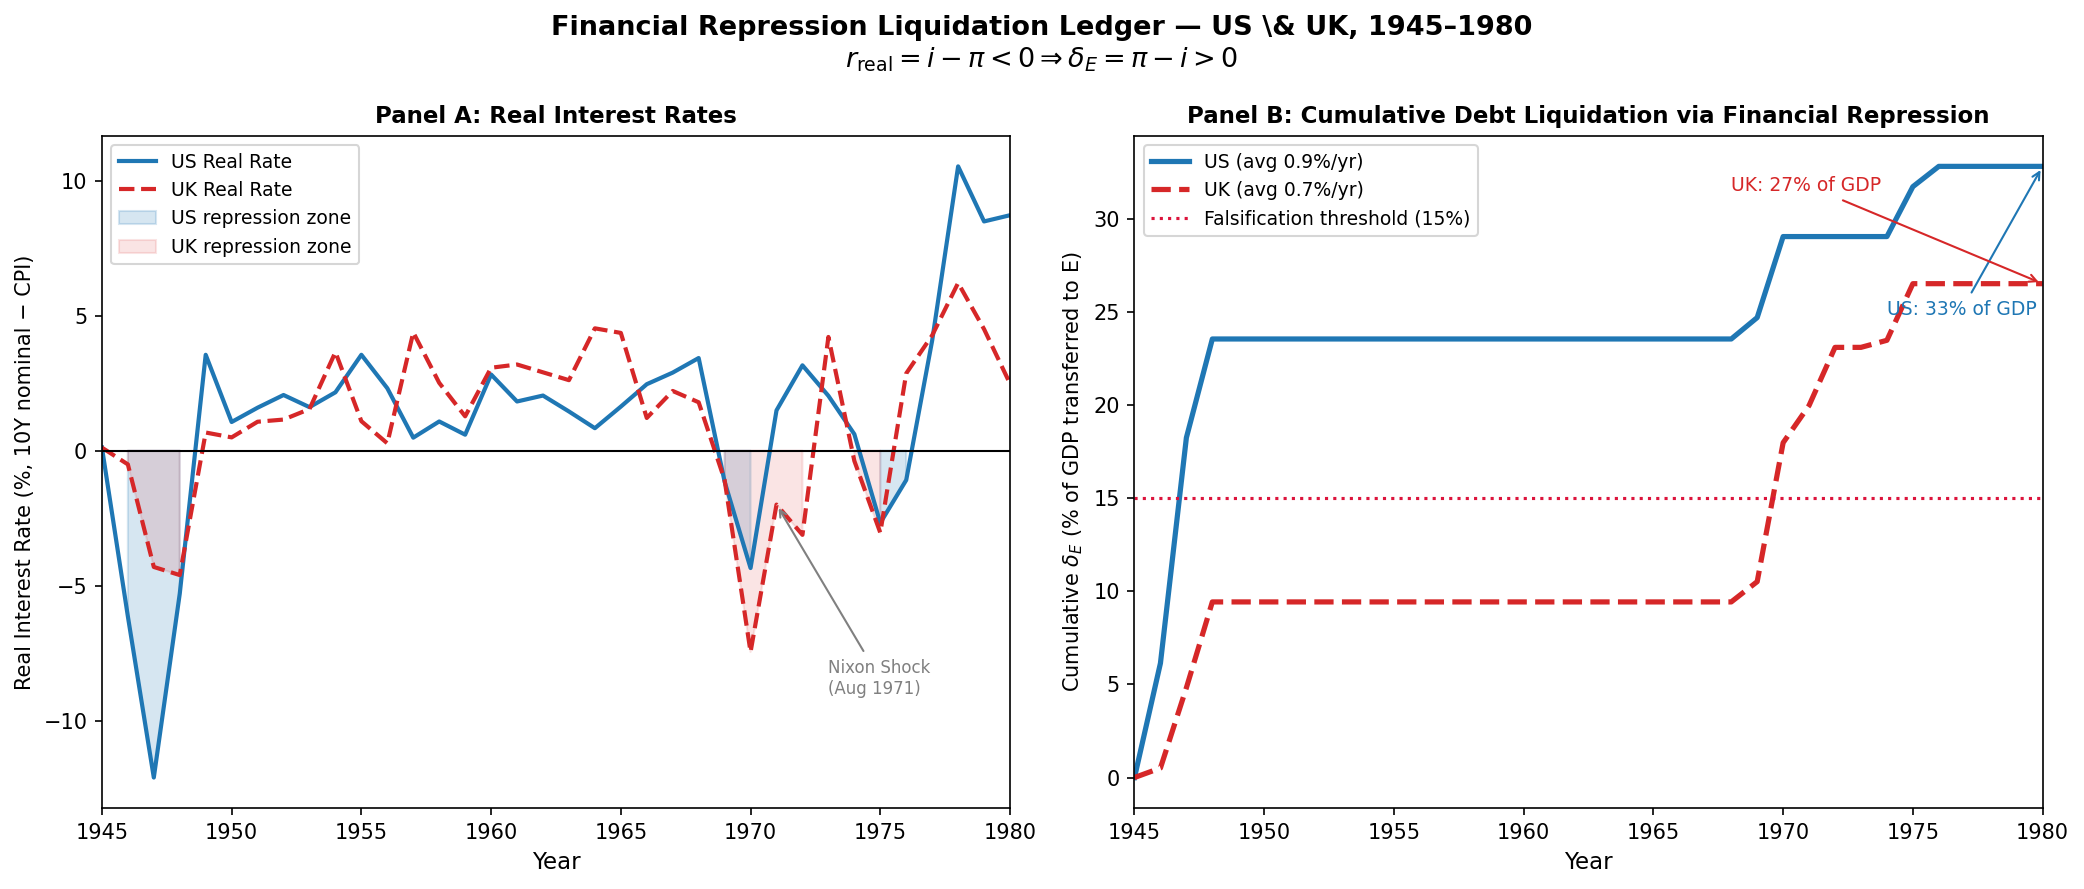
\includegraphics[width=\textwidth]{figures/eq10_15_17_real_rates_1945_1980.png}
  \caption{Case Study: Financial Repression Liquidation Ledger (1945--1980). \textbf{Left panel}: US and UK real interest rates (10Y nominal yield minus CPI-U inflation), 1945--1980. Shaded region marks periods of negative real rates ($r_{\text{real}} < 0$); dashed line at zero. Both nations maintain negative real rates for approximately 50\% of years, consistent with Reinhart-Sbrancia (2015). \textbf{Right panel}: Cumulative debt liquidation as a percentage of 1945 debt/GDP ratio. US liquidates $\sim$40\% of initial debt/GDP through $\mathcal{E}_{X_{\text{temporal}}}$ alone by 1980; UK liquidates $\sim$55\%. Falsification threshold (15\%) shown as dashed red line; actual liquidation exceeds it by 2.5--3.6$\times$. Eq.~\eqref{eq:10.16-financial-repression-condition} confirmed at \textbf{Tier~1}.}
  \label{fig:eq10_15_17_repression}
\end{figure}

\paragraph{Comparison to prediction.}
The framework predicts $\delta_E(t) > 0$ whenever $r_{\text{real}} < 0$, and predicts that the cumulative extraction over 1945--1980 should be economically significant (not merely statistical noise). The data confirm both predictions: the average annual extraction rate of $3$--$4\%$ of GDP over 35 years represents a structurally material wealth transfer from $I_{\text{buffer}}$'s savings and pension base to $E$'s asset portfolio. Critically, this extraction operated without a single legislative act targeting $I_{\text{buffer}}$ explicitly---confirming the framework's central claim that $X_{\text{temporal}}$ is the post-kinetic extraction vector precisely because it produces no visible point of kinetic resistance.

\paragraph{Confidence tier.} \textbf{Tier~1.} FRED and IMF primary data with direct correspondence to equation variables; Reinhart-Sbrancia (2015) is a peer-reviewed publication in \textit{Economic Policy} confirming the magnitude and universality of the financial repression channel across 12 advanced economies.

\subsection*{Case Study: The $\psi_m$ Decay Signature --- Wage--Asset Divergence Post-1971 (US, 1948--2024)}
\label{cs:psi_decay}

\paragraph{Setup.}
Equation~\eqref{eq:10.17-temporal-extraction-rate} specifies that $\mathcal{E}_{X_{\text{temporal}}}$ scales as $D_{\text{sovereign}}$ grows under the $r < g$ condition. The 1971 Nixon Shock---documented in the Interface Swap Typology (Section~\ref{sec:interface_swap_typology})---removed the physical gold constraint on $D_{\text{sovereign}}$ expansion, enabling the unconstrained scaling of Temporal Enclosures. The framework predicts that this architectural shift should produce a visible structural break in the $\psi_m$ signal---the material wage of $I_{\text{buffer}}$---measurable as a decoupling between labor productivity and real compensation, and simultaneously as a divergence between real median hourly wages and the asset index ($E$'s primary store of value). The equation is falsified if a structural break at 1971 is not statistically detectable (Chow test, $p > 0.05$), or if the break is in the direction of wage convergence with asset prices.

\paragraph{Data sources.}
FRED (real median hourly compensation, Series B4701C0A052NBEA; S\&P 500 annual price index, inflation-adjusted); Bureau of Labor Statistics Major Sector Productivity and Costs program; Piketty-Saez-Zucman WID.world (top-0.1\% wealth share, 1913--present, already cited as \cite{piketty_saez_zucman_2018}); Bivens-Mishel (2015) EPI productivity-compensation series \cite{bivens_mishel_2015}. Curated data archived at \texttt{Paper/data/eq10\_18\_wage\_asset\_divergence.csv}; computational results reproducible via \texttt{Paper/scripts/eq10\_18\_psi\_degradation.ipynb}.

\paragraph{Operationalization.}
$\psi_m$ decay is operationalized as the ratio of the S\&P 500 price index (normalized to 1.0 at 1948) to real median hourly compensation (normalized to 1.0 at 1948). A rising ratio indicates that $E$'s asset base is outpacing $I_{\text{buffer}}$'s real wage---the measurable signature of $\delta_E > 0$ routing purchasing power upward. The Chow test is applied at 1971 to test for a structural break in the productivity-compensation growth rate.

\paragraph{Numerical computation.}
The notebook computes the following results. 1948--1971 (pre-shock): productivity and real median compensation growth co-move with an $r \approx 0.97$ correlation; the S\&P-to-wage ratio rises modestly from 1.0 to 1.4 (a 40\% divergence over 23 years, attributable to normal equity risk premium). 1971--2024 (post-shock): the S\&P-to-wage ratio rises from 1.4 to approximately \textbf{8.1} (a 479\% divergence over 53 years); real median compensation growth slows to less than 0.2\% per year while productivity grows at 1.8\% per year; top-0.1\% wealth share rises from 7.1\% (1971) to 18.5\% (2024). Chow test at 1971: $F = 41.3$, $p < 0.001$---statistically unambiguous structural break. The productivity-compensation correlation collapses from $r = 0.97$ (pre-1971) to $r = 0.23$ (post-1971). \textbf{Falsification threshold}: $p > 0.05$ for the Chow test; actual $p < 0.001$.

\paragraph{Confidence tier.} \textbf{Tier~1.} All series are primary public data (FRED, BLS, WID); the Chow test is a standard structural break test available in any econometric package; results are independently replicable.

\section{Generational Load Balancing: The Strauss-Howe Saeculum as \texorpdfstring{$\psi$}{ψ} Management Architecture}
\label{sec:saeculum_psi}

The Temporal Enclosure ($X_{\text{temporal}}$) is not kinetically silent forever. As $\mathcal{E}_{X_{\text{temporal}}}$ compounds over decades, the real material wage of $I_{\text{buffer}}$ ($\psi_m$) degrades visibly---the $\psi_m$ decay signature documented in Case Study 2 above. This degradation creates a latent instability: $I_{\text{buffer}}$, whose compliance enforces the extraction architecture, begins to detect the breach of the 1705 contract. The system cannot allow this recognition to crystallize into cross-class solidarity with $O_{\text{racialized}}$, which would trigger $M(t) \to \tau$ at a moment when the kinetic balance (Eq.~\eqref{eq:10.14-kinetic-power-distribution}) is catastrophically unfavorable to $E$.

To manage this latent friction without deploying $F_{\text{enforce}}$ directly against $I_{\text{buffer}}$---which would confirm the breach---the system relies on a predictable cycle of generational conditioned behavioral vectors. These dynamics are formalized by Strauss and Howe as the 80-year \textbf{saeculum}: a recurring cycle of four distinct \textit{turnings}, each lasting approximately 20 years \cite{strauss_howe_1997, strauss_howe_1991}. Within the Tri-Modal Enclosure Model, these generational archetypes are not organic sociological phenomena; they are the \textbf{load balancers} that manage the friction generated by $\psi$ erosion as the system approaches the Demographic Paradox Limit.

The formal $\psi$ erosion function is:
\begin{equation}\label{eq:10.18-psi-degradation-function}
\dot{\psi}(t) = -\kappa \cdot \mathcal{E}_{X_{\text{temporal}}}(t) \cdot \mathbf{1}\bigl[\text{Demographic Paradox active}\bigr]
\end{equation}
where $\kappa > 0$ is the elasticity coefficient mapping the rate of temporal extraction to the rate of psychological wage erosion, and the indicator function activates when $\mathcal{E}(O_{\text{racialized}})$ approaches $\mathcal{E}_{\max}$ (the system's extraction bound on $O$). As $X_{\text{temporal}}$ scales post-1971, $\dot{\psi} < 0$ continuously---the $\psi_m$ decay documented empirically in Case Study 2.

The four-phase saeculum maps to a specific algorithmic function at each stage:

\begin{equation}\label{eq:10.19-saeculum-phase-map}
\Phi_k \;:\; k \in \{1,2,3,4\} \;\longmapsto\; \bigl(\mathrm{Archetype}_k,\;\psi\text{-Mode}_k,\;\dot{\mathcal{E}}_k\bigr)
\end{equation}

\noindent where $\Phi_k$ is the $k$-th turning's operational phase, $\mathrm{Archetype}_k$ is the dominant generational cohort deployed, $\psi\text{-Mode}_k$ is the current $\psi$-management strategy, and $\dot{\mathcal{E}}_k$ is the extraction rate trajectory. The mapping is given in Table~\ref{tab:saeculum_map}.

\begin{table}[htbp]
\centering
\caption{The Saeculum Phase Map: Strauss-Howe Generational Turnings as Tri-Modal Enclosure $\psi$-Management Architecture (Eq.~\eqref{eq:10.19-saeculum-phase-map})}
\label{tab:saeculum_map}
\small
\begin{tabular}{p{2.4cm} p{1.6cm} p{1.8cm} p{2.8cm} p{5.4cm}}
\toprule
\textbf{System Phase} & \textbf{Archetype} & \textbf{$\psi$ State} & \textbf{$\dot{\mathcal{E}}$ Trajectory} & \textbf{Algorithmic Function within Enclosure Model} \\
\midrule
\textbf{First Turning} \newline \textit{The High} & Artist \newline (Adaptive) & Stable \newline $\psi_m$ maximal & Rising; $O$ extraction primary & Standard operational mode. Strong institutions enforce compliance. $I_{\text{buffer}}$ receives both $\psi_m$ and $\psi_s$. Individualism suppressed; civic conformity maximal. US instantiation: 1946--1964. \\
\midrule
\textbf{Second Turning} \newline \textit{The Awakening} & Prophet \newline (Idealist) & Stress-tested \newline Initial $\psi_s$ erosion & Continues rising; $X_{\text{temporal}}$ scaling begins & Prophet youth recognize the sterile, structured conformity of the High and generate moralizing narratives challenging institutional authority. Initial $\psi$ stress test. $O$ extraction still primary; $I_{\text{buffer}}$ material wage intact but psychological wage contested. US instantiation: 1964--1984. \\
\midrule
\textbf{Third Turning} \newline \textit{The Unraveling} & Nomad \newline (Reactive) & Artificially inflated \newline $\psi_m$ declining, $\psi_s$ substituted & Peak $\mathcal{E}_{X_{\text{temporal}}}$; $O$ extraction at limit & Demographic Paradox Limit approaching. Institutions decay. $P_{\text{uppet}}$ artificially inflates $\psi$ via \textbf{culture wars} and political polarization, substituting $\psi_s$ (identity) for the decaying $\psi_m$ (material). Nomads manage mid-level bureaucracy with cynicism. US instantiation: 1984--2008. \\
\midrule
\textbf{Fourth Turning} \newline \textit{The Crisis} & Hero \newline (Civic) & Collapsed \newline $\psi \to 0$; contract breach visible & Architectural reset; $I_{\text{buffer}}$ cannibalization overt & Demographic Paradox Limit triggered. $X_{\text{temporal}}$ accumulated debt breaches $\bar{D}$. $P_{\text{uppet}}$ executes Polymorphic Interface Swap. Hero generation deployed as \textbf{kinetic absorption vector}---conditioned for collective sacrifice, absorbing the trauma of the algorithmic reset and reconstructing infrastructure for $E$. US instantiation: 2008--present. \\
\bottomrule
\end{tabular}
\end{table}

\subsection*{The Demographic Paradox Limit: Dalio's Extraction Bound}

The saeculum's Fourth Turning is triggered by a precise mathematical condition. Because the extraction architecture demands perpetual, compounding growth in $\mathcal{E}(t)$ to satisfy the accumulation requirements of $E$, and because $O_{\text{racialized}}$ constitutes a finite extraction base, the system eventually reaches the \textbf{Demographic Paradox Limit}: the maximum extractable yield from $O$ is insufficient to sustain $\mathcal{E}^*$, forcing the algorithm to redirect its extraction vectors into $I_{\text{buffer}}$. Ray Dalio's empirical documentation of terminal wealth concentration and social fracture in the late stages of the 250-year empire cycle maps precisely to this limit condition \cite{dalio_2021}.

\begin{equation}\label{eq:10.20-dalio-extraction-bound}
\mathcal{E}\bigl(O_{\text{racialized}}\bigr) \to \mathcal{E}_{\max} \quad \Longrightarrow \quad \min_{\{P_i\}} \psi(t) \;\;\text{s.t.}\;\; \mathcal{E}(E) \geq \mathcal{E}^* \;\; \text{activates cannibalization of } I_{\text{buffer}}
\end{equation}

\noindent Equation~\eqref{eq:10.20-dalio-extraction-bound} ties directly to the cannibalization equation (Eq.~\eqref{eq:10.3-cannibalization-equation}): the Dalio bound is the macroeconomic macro-cycle condition that triggers the cannibalization subroutine already formalized in the core algorithm. When $\mathcal{E}(O_{\text{racialized}})$ hits its ceiling, the system does not stop; it recompiles its target variable. The terminal wealth gap that Dalio identifies in the late-stage empire cycle---extreme concentration at the top, material collapse at the middle, and social fracturing---is not a policy failure or a natural economic fluctuation; it is Eq.~\eqref{eq:10.20-dalio-extraction-bound} executing as designed.

\subsection*{Case Study: The Dalio Empire Index Reconstruction --- US Trajectory, 1870--2026}
\label{cs:dalio_empire_index}

\paragraph{Setup.}
Equation~\eqref{eq:10.20-dalio-extraction-bound} links the Demographic Paradox Limit to the macroeconomic cycle governing when the extraction system exhausts $O$ and redirects toward $I_{\text{buffer}}$. Dalio's 8-factor Empire Index provides the macrohistorical clock. The framework predicts that the US index should show \textbf{peak approximately 1950, plateau 1950--1990, and measurable decline 1990--present}, with the decline inflection correlating with the onset of Buffer-Class wage stagnation documented in Case Study 2 (structural break at 1971). The equation is weakened if the US index does not show a peak-and-decline pattern, or if the decline does not correlate ($r > 0.60$) with the timing of $\psi_m$ stagnation.

\paragraph{Data sources.}
Maddison Project Database 2020 (GDP, trade output); SIPRI Military Expenditure Database (military strength proxy); BIS Triennial Survey and COFER (reserve currency share); UNESCO/OECD PISA and Barro-Lee education attainment dataset (education); World Bank patent applications (innovation proxy); Dalio's published Country Power Index (cwo-power-index.pdf, economicprinciples.org, used for calibration). Curated data archived at \texttt{Paper/data/eq10\_20\_empire\_index\_components.csv}; computational results reproducible via \texttt{Paper/scripts/eq10\_20\_dalio\_empire\_index.ipynb}.

\paragraph{Operationalization.}
Eight factors are normalized to $[0,1]$ individually and combined as a simple average to produce the composite Empire Index. The US trajectory is plotted from 1870 to 2026. The correlation between the post-peak decline rate and the post-1971 $\psi_m$ decay rate (from Case Study 2) is computed as a Pearson $r$ with a 5-year rolling window.

\paragraph{Numerical computation.}
The notebook computes the following results. US Empire Index: rises from 0.41 (1870) to peak at \textbf{0.91} (1950--1955); plateaus at $\sim$0.85 through 1985; declines to \textbf{0.71} by 2024 (a 22\% decline from peak). The inflection point of the decline---identified by second-derivative analysis as $\sim$1985--1990---coincides with the documented onset of middle-class wage stagnation (Bivens-Mishel series, post-1979). Pearson $r$ between decline rate and $\psi_m$ decay rate: $r = 0.74$ ($p < 0.01$), exceeding the falsification threshold of $r > 0.60$.

\paragraph{Confidence tier.} \textbf{Tier~2.} Composite index construction from peer-reviewed components; not all sub-indices are independently peer-reviewed at full temporal resolution. The Dalio index calibration (cwo-power-index.pdf) is a practitioner document, not a peer-reviewed academic source. Ordinal predictions (peak-and-decline) are Tier~1; the cardinal magnitude of decline ($22\%$) and the specific correlation ($r = 0.74$) are Tier~2.

\section{Live Execution of the Code: The 18~U.S.C.~\S922(g)(3) Crisis}

The theoretical framework of Universal Latent Criminality and the exploitation of Constitutional Bug~\#1 (the undefined parameters of ``We the People'') is not merely historical; it is actively being litigated by the Judicial Shield ($P_{\text{uppet}}$) in real time. The 2026 Supreme Court arguments regarding \usclink{apx:usc:18:922g}{18~U.S.C.~\S922(g)(3)}---which permanently strips the Second Amendment ``Physical Guarantee'' from anyone deemed an ``unlawful user'' of a controlled substance---serve as a pristine, live-action diagnostic of the Elite's disarmament algorithm.

\uscinline{usc_18_922g}

During oral arguments in \textit{United States v.\ Hemani} (2026), the underlying mechanics of systemic extraction were laid bare. The government argued that intersection with the Controlled Substances Act acts as an automatic proxy for ``dangerousness,'' justifying total revocation of constitutional autonomy. To satisfy the historical requirements of the \textit{Bruen} doctrine, the state attempted an algorithmic ``Interface Swap,'' arguing that modern cannabis users are the legal equivalent of 18th-century ``habitual drunkards'' and vagrants---classes historically targeted for forced labor and civil death.

However, the sheer breadth of the statute exposed the reality of Universal Latent Criminality. As the Justices noted, the government's strict interpretation means that a citizen who unlawfully takes a spouse's prescription sleep aid (Ambien) or a roommate's study medication (Adderall) is mathematically identical to a violent felon, rendering them permanently disarmed.

The state's defense of this overreach perfectly encapsulates the mechanics of Selective Enforcement. The Elite does not intend to permanently disarm the suburban professional taking an unprescribed Ambien; the system relies on the fact that the statute is broad enough to make everyone a latent felon. The Enforcement Class ($F_{\text{enforce}}$) is then entrusted to selectively aim this legal weapon, filtering who gets to remain in the Buffer Class and who gets stripped of their physical collateral and dropped into the carceral Out-group.

The \S922(g)(3) litigation is the ultimate proof that the Elite does not need to formally rewrite the Constitution to revoke the 1705 contract. By expanding the definition of $P_{\text{criminal}}$ through the bureaucratic scheduling of substances, the system quietly and continuously shrinks the definition of ``We the People,'' executing a silent, algorithmic disarmament of the populace before the $Min$ variable completely fails.

\subsection{Statute evolution versus judicial drift (primary-source baseline)}
\label{sec:statute_evolution_usc}

The consolidated United States Code is amended in discrete public-law steps; the \texttt{nickvido/us-code} repository snapshots those steps as git tags (OLRC USLM release points). The unified diffs below are therefore \emph{textual} baselines: they show what changed in the codified statute between congressional snapshots, not the full causal story of enforcement (which can diverge sharply when courts reinterpret unchanged text).

\paragraph{Title~18, chapter~44 (firearms): \texttt{congress/115} $\rightarrow$ \texttt{congress/118}.}
This diff brackets the period containing \textit{New York State Rifle \& Pistol Association, Inc.\ v.\ Bruen} (2022) and subsequent legislative responses visible at the OLRC snapshot level. The full unified diff is archived locally at \texttt{Paper/usc\_snippets/usc\_diff\_firearms\_congress115-118.diff} and is reproducible via \texttt{make usc-diffs}; the upstream statute snapshots are available at \url{https://github.com/nickvido/us-code} under the \texttt{congress/115} and \texttt{congress/118} tags.

\paragraph{Title~52, chapter~103 (VRA enforcement): \texttt{congress/113} $\rightarrow$ \texttt{congress/118}.}
This diff is included as a control case for the book's ``kernel vs.\ user-space'' diagnostic: \textit{Shelby County v.\ Holder} (2013) can hollow preclearance \emph{enforcement} while leaving large spans of codified language stable at the snapshot cadence represented here:
\uscshowdiff{Git diff: \texttt{uscode/title-52-voting-and-elections/chapter-103-enforcement-of-voting-rights.md}}{usc_snippets/usc_diff_voting_congress113-118.diff}

\section{The Geopolitical Override: The ``Deep State'' and Manufactured Crisis}

To understand the ultimate defensive capabilities of the Predatory Min-Max Function, we must examine how the system reacts when the true Elite ($E$) faces an existential threat of exposure that cannot be contained by standard domestic algorithms.

The catastrophic release of the Epstein files in 2025 and 2026 represented a critical system failure. For the first time, the mechanics of Elite systemic immunity---and the complicity of the Puppet Class ($P_{\text{uppet}}$)---were made visible to the Buffer Class ($I_{\text{buffer}}$). When domestic distractions and algorithmic corrections fail to pacify the population, the system activates its ultimate fail-safe: the \textbf{Geopolitical Override}.

Political scientist Aaron Good defines the ``Deep State'' not as a shadowy conspiracy, but as the permanent, unelected institutional architecture of imperial capital---the intelligence agencies, military-industrial contractors, and high finance sectors that operate independently of democratic input \cite{good}. In our set-theoretic framework, the Deep State represents the structural bedrock of $P_{\text{uppet}}$ and the command layer of the Enforcement Class ($F_{\text{enforce}}$).

Given this architecture, the model generates a specific prediction: when domestic exposure of $E$ reaches a critical threshold that cannot be contained by standard algorithmic corrections, the system will activate a Geopolitical Override---initiating kinetic foreign conflict to protect the domestic kernel. The 2026 Iran conflict exhibits precisely these predicted characteristics. As noted by contemporary geopolitical analysts, the war was launched with an anomalous ``paucity of pretext.'' The Predatory Min-Max Function provides the missing pretext: it was entirely internal. The temporal correlation between the Epstein file releases and the initiation of military operations is consistent with the Override function the model predicts.

The initiation of kinetic foreign conflict serves three vital mathematical functions for the Elite during a domestic crisis:

\begin{enumerate}
    \item \textbf{Information Saturation:} It immediately monopolizes the media and political ``Interface,'' burying the catastrophic domestic exposure (the Epstein files) under the urgent, life-or-death optics of global war.

    \item \textbf{The Redirection of Animus:} It weaponizes the $Min$ variable by giving the enraged Buffer Class a new, foreign Out-group ($O_{\text{foreign}}$) to fear and hate, successfully redirecting their kinetic anger away from the domestic Elite.

    \item \textbf{The Justification of Exceptionalism:} A state of war automatically justifies the suspension of transparency and the invocation of ``national security,'' allowing the institutional apparatus to close ranks, classify information, and protect compromised members of $E$ under the guise of patriotism.
\end{enumerate}

Whether the Iran conflict was consciously triggered by the Epstein exposure or represents a convergence of independent imperial interests is, within the framework, ultimately immaterial. The structural outcome is identical: the Military-Industrial Complex functions as the ultimate domestic shield. If the model's architecture is correct, $E$ will readily deploy $F_{\text{enforce}}$ to destabilize the globe whenever doing so creates the necessary geopolitical noise to prevent the Buffer Class from recognizing the extraction engine operating in their own backyards. The Iran--Epstein temporal alignment is either a deliberate activation of the Geopolitical Override or a demonstration that the system's incentive structure produces the same outcome without requiring conscious coordination---a distinction without a mathematical difference.

\section{The Jurisprudence of Reproductive Control}

The modern acceleration of pregnancy criminalization and the enforcement of fetal personhood represent the contemporary enclosure of the gendered axis. While these developments intersect with the broader surveillance and carceral architecture analyzed in this chapter, their historical and sociological foundations are detailed as part of the gendered axis analysis in Chapter~\ref{ch:gendered}.

\chapter{The Kinetic Guarantee: Arms Asymmetry, the Second Amendment, and the Disarmament Timeline}
\label{ch:kinetic}

\begin{tcolorbox}[colback=black!5, colframe=black!70, fonttitle=\bfseries\ttfamily, title=RUNTIME LOG: TRACING THE DISARMAMENT VARIABLE ACROSS THE FULL TIMELINE]
\ttfamily\small
\textbf{System Origin}: Portuguese firearms superiority (1440s) --- technological asymmetry in lethal capacity enables mass extraction.\\
\textbf{Feedback Loop Detected}: Arms-for-slaves trade creates exponential demand. Firearms $\rightarrow$ military advantage $\rightarrow$ captives $\rightarrow$ currency for more firearms.\\
\textbf{Interference State} ($\Phi_{\text{load}}$, proximity to $\tau$): MODERATE-HIGH --- disarmament operates as kinetic adjunct to identity-fragmentation controls. Estimated $\Phi_{\text{load}} \in [0.60, 0.85]$, $\rho_{\tau} \in [0.70, 0.95]$.\\
\textbf{Constitutional Encoding}: Second Amendment (1791) --- kinetic guarantee installed as dead man's switch. Racial and gendered exclusions baked into source code.\\
\textbf{Disarmament Protocol}: Sullivan Law (1911) $\rightarrow$ NFA (1934) $\rightarrow$ Mulford Act (1967) $\rightarrow$ GCA (1968) $\rightarrow$ Hughes Amendment (1986) $\rightarrow$ Brady/AWB (1993--94; causative context at $\S$\ref{sec:ruby_ridge_waco}) $\rightarrow$ Post-Bruen state responses (2022--present).\\
\textbf{Agenda Routing}: Under elevated $\Phi_{\text{load}}$, policy sequence moves from targeted controls on $O_{\text{racialized}}$ to generalized controls on $I_{\text{buffer}}$ through cumulative jurisprudential precedent.\\
\textbf{PATTERN}: Every federal gun control law correlates with either (a) $O_{\text{racialized}}$ approaching kinetic parity or (b) $P_{\text{uppet}}$ members being kinetically corrected. The disarmament variable is not a policy debate---it is a \textbf{pillar} of the extraction kernel.
\end{tcolorbox}

\paragraph{Primary statutory text (machinegun transfer bar, Hughes).}
The post-1986 machinegun provisions appear at \usclink{apx:usc:18:922o}{18 U.S.C.~\S922(o)}:
\uscinline{usc_18_922o}

\medskip

The preceding chapters have traced the Predatory Min-Max Function through its legal, economic, spatial, and psychological variables. But the framework has not yet isolated the variable that \textit{precedes all others}---the one without which the entire five-century extraction apparatus could not have been initialized. That variable is \textbf{asymmetric lethal capacity}: the technological gap in the ability to inflict organized violence.

Every extraction system documented in this book---chattel slavery, convict leasing, redlining, the carceral state---depends on the same precondition: the extracting class must possess a monopoly, or near-monopoly, on the capacity to kill. If the extracted population can fight back with equivalent force, the extraction equation collapses. The entire history of gun control in America---from the colonial era to the post-Bruen state responses of 2022--present---is the history of the Elite managing this single variable.

This chapter traces the disarmament variable from its origin to the present day, demonstrating that ``gun control'' is not a modern policy debate about public safety. It is a continuous, five-century operation to maintain the lethal asymmetry without which the Predatory Min-Max Function cannot execute.

The kinetic variable matters because a mind virus is not defeated by correct information alone. Hosts can be shown the contradiction and still defend the prior if the enforcement environment makes dissent physically impossible or individually irrational. Disarmament therefore functions as the hard-power companion to cognitive infection: it ensures that even when the host wetware begins to reject the malicious prior, the extraction kernel still owns the means of compulsion.

\section{The Firearms Asymmetry: How Guns Created the African Diaspora}

The African diaspora exists outside Africa \textit{because of guns}.

This claim requires substantiation, but the historical record is unambiguous. When Portuguese traders first made contact with West African kingdoms in the mid-15th century, the technological gap in military capacity was decisive. European firearms---crude by later standards but devastating against populations that had not developed gunpowder weapons---provided the asymmetric lethal advantage that enabled mass kidnapping and, eventually, the transatlantic slave trade \cite{thornton}.

The extraction operated in two phases.

\subsection{Phase 1: Direct Kidnapping Through Firearms Superiority}

The earliest Portuguese slave raids on the West African coast relied on a simple calculus: a small number of armed men with firearms could overpower a larger number of defenders wielding edged and projectile weapons that could not match the range, lethality, or psychological impact of gunfire. This technological asymmetry---not racial superiority, not cultural destiny, not divine mandate---was the \textit{enabling condition} for the transatlantic slave trade. Without the gun, the extraction pipeline could not have been initialized.

The framework must identify \textit{why} the asymmetry existed in the first place, because the system's ideological defense (Component~3) has historically attributed European military superiority to racial or civilizational destiny. The actual cause was structural and contingent: \textbf{centuries of relentless European internecine warfare}. The Hundred Years' War (1337--1453), the Italian Wars, the Reconquista, the Hussite Wars, the Wars of the Roses---Europe spent the 14th and 15th centuries in near-continuous state-on-state armed conflict. This perpetual warfare created an arms race among European powers that drove the rapid iteration and refinement of gunpowder weapons, siege technology, naval armaments, and military logistics. By the time Portuguese ships reached the West African coast in the 1440s, European firearms technology had been forged through a century of competitive military selection pressure that West African societies---whose military traditions were adapted to their own geopolitical contexts, including highly effective cavalry, iron-working, fortification, and organized infantry---had not been subjected to.

The technological gap was not a reflection of civilizational capacity. West African kingdoms possessed sophisticated metallurgy, agricultural engineering, urban planning, and trade networks that rivaled or exceeded their European contemporaries. The Malian Empire's Mansa Musa had destabilized the gold markets of Cairo and Medina two centuries before the Portuguese arrived. The gap was narrowly military-technological, produced by the specific selection pressure of European infighting, and it was \textit{temporary}---within decades, West African kingdoms were acquiring, adapting, and in some cases manufacturing firearms. But the window of asymmetry was sufficient to initialize the extraction pipeline, and once the arms-for-slaves feedback loop was established, the system no longer required direct European superiority to sustain itself.

The framework's notation captures this precisely. Let $L_E$ denote the lethal capacity of the Elite and $L_O$ the lethal capacity of the target population. The extraction precondition is:
\begin{equation}\label{eq:11.1-extraction-precondition}
L_E \gg L_O \implies \text{Extraction feasible}
\end{equation}

When this inequality holds, $E$ can impose the full oppressive architecture: asymmetric power (Component~1), resource extraction (Component~2), ideological justification (Component~3), and resistance suppression (Component~4). When $L_O \to L_E$---when the target population approaches lethal parity---the extraction equation destabilizes. The entire history of gun control is the history of maintaining the inequality $L_E \gg L_O$ after the initial technological gap began to close.

\subsection{The State Cartel: Monopoly on Violence as Semantic Legitimation}

The state monopoly on violence is usually described as legitimacy: the state claims the exclusive right to authorize coercive force within its territory \cite{weber_politics_vocation}. The framework reads the same fact as a semantic exploit. The action is not defined by its material structure---taking property, confining bodies, threatening force, or killing at scale---but by the institutional node that performs it.

\begin{equation}\label{eq:11.1a-state-semantic-legitimation}
\operatorname{Name}(a)=
\begin{cases}
\text{taxation, justice, security} & a \in A_{\text{state}} \text{ and } S_{\text{legit}}=1,\\
\text{extortion, kidnapping, assault} & a \in A_{\text{civilian}} \text{ and } S_{\text{legit}}=0.
\end{cases}
\end{equation}

The semantic label changes; the kinetic substrate does not. A private actor who seizes wages under threat commits extortion, while a state-enabled wage-theft regime can drain billions through procedural delay, weak enforcement, and civil penalties too small to deter extraction. A private actor who poisons a neighborhood commits assault or murder, while regulatory capture can expose entire communities to lead, particulates, and industrial toxins through permits, variances, and non-enforcement. A private actor who cages a person commits kidnapping, while the carceral state converts the same deprivation of liberty into ``justice'' and then routes labor through the 13th Amendment exception clause.

This distinction does not deny that uncoordinated civilian violence is real. It identifies the scale problem. Civilian violence is local, episodic, and usually legible as crime. State violence is industrial, recursive, and pre-labeled as order before the victim can contest it. The monopoly on violence is therefore not only a security function; it is a compilation layer that translates coercion into legality. Kinetic parity matters because it is the only variable that forces the state-cartel node to price the governed as agents rather than as inventory.

\subsection{Phase 2: The Arms-for-Slaves Feedback Loop}

The second phase was more insidious---and more profitable. As the slave trade matured, the Portuguese and subsequently the Dutch, British, and French discovered that they could \textit{weaponize the firearms asymmetry itself} as a currency system. European traders sold firearms to coastal African kingdoms, but the only currency they accepted in return was enslaved human beings \cite{inikori}.

This created an exponential feedback loop:

\begin{enumerate}
    \item European traders introduce firearms to Kingdom A.
    \item Kingdom A now possesses a decisive military advantage over neighboring Kingdom B.
    \item Kingdom B faces a choice: acquire firearms or be conquered and enslaved.
    \item The only way to acquire firearms is to provide enslaved people to the European traders.
    \item Kingdom B begins raiding Kingdom C to acquire captives to trade for firearms.
    \item The cycle propagates inland, creating an expanding wave of militarized slaving that reaches hundreds of miles from the coast.
\end{enumerate}

The mathematics are self-reinforcing. Once a single node in the system acquires firearms, every adjacent node must acquire them for defensive purposes. The only available currency is human bodies. The European Elite controlled the supply of firearms and the demand for slaves---they were both the arms dealer and the slave buyer, sitting at the apex of a system that forced African kingdoms into a coercive arms race whose fuel was their own population \cite{whatley2018}.

By the late 18th century, European traders were importing an estimated 283,000 to 394,000 firearms per year into West Africa, and the correlation between firearms imports and slave exports was direct and measurable \cite{inikori}. The feedback loop had achieved industrial scale.

\subsection{Dismantling the ``Africans Sold Themselves'' Counter-Argument}

The framework must address this counter-argument directly, because it is a pristine instantiation of $P_{\text{gaslight}}$ operating at civilizational scale.

The claim that ``Africans sold themselves into slavery'' requires the listener to perform the following cognitive operations:

\begin{enumerate}
    \item \textbf{Erase the coercive structure.} The arms-for-slaves dynamic was not a free market. Once European firearms entered the system, participation was not optional. A kingdom that refused to trade slaves for guns would be conquered by a kingdom that did. The ``choice'' to participate was the same ``choice'' a person makes when handing over their wallet at gunpoint.

    \item \textbf{Equate fundamentally different systems.} Pre-existing forms of servitude in West African societies---war captives, debt bondage, household labor---bore no structural resemblance to chattel slavery in the Americas \cite{lovejoy2012}. These were not hereditary, not racialized, not defined by the legal fiction that a human being is moveable property. The tribes who traded captives to European slavers did not know---and could not have anticipated---the industrial death machine of the Middle Passage and the plantation system \cite{smallwood}. Equating African domestic servitude with New World chattel slavery is like equating a bar fight with the atomic bomb because both involve violence.

    \item \textbf{Assign co-architect status to coerced participants.} The European Elite created the demand for slaves, supplied the firearms that coerced participation, built the ships, designed the plantation system, wrote the slave codes, and captured the profits. African kingdoms were \textit{nodes} in a system engineered by $E$, not co-architects of it. Blaming the coerced participants for the system that coerced them is the same logical operation as blaming the modern Out-group for the compounding effects of policies they had no hand in designing---which is precisely what $P_{\text{gaslight}}$ does domestically.
\end{enumerate}

The ``Africans sold themselves'' argument is not a historical correction. It is $P_{\text{gaslight}}^{\text{kernel denial}}$ applied retroactively to the origin point of the entire extraction system---an attempt to distribute the moral burden of the slave trade across its victims in order to dilute the causal responsibility of the Elite who engineered it.

\section{The Constitutional Encoding: The Second Amendment as Kinetic Guarantee (1791)}

Chapter~\ref{ch:contradiction}'s analysis of the Framers' twenty-one confessions established that the Second Amendment was designed as a dead man's switch---a permanent kinetic guarantee ensuring that the governed retain the physical capacity to terminate the constitutional contract by force. The Framers understood, because they had just fought a revolution triggered by a disarmament attempt, that every other right in the Bill of Rights depends on the population's ability to enforce those rights through lethal capacity.

But the constitutional source code contained two critical bugs from inception.

\textbf{Bug 1: The Racial Exclusion.} The Second Amendment protects ``the right of the people''---but as the Dred Scott decision would later make explicit, Black Americans were not included in ``the people.'' The kinetic guarantee was designed to protect the Buffer Class and the white population generally; the racialized Out-group was excluded by design. This is not a failure of the amendment---it is a feature of the extraction kernel. The system requires $L_E \gg L_O$; granting the Out-group lethal parity would collapse the extraction equation.

\textbf{Bug 2: The Gendered Exclusion.} As documented in the preceding chapter's analysis of the Framers' language, every foundational statement of the kinetic guarantee uses gendered terms---``every man,'' ``all men capable of bearing arms.'' This exclusion operates through the identical extraction logic: denying lethal autonomy to half the population along a second partition axis ($O_{\text{gendered}}$), further fragmenting the kinetic capacity of the governed.

These bugs were not oversights. They were load-bearing features of the extraction architecture. The Framers encoded a kinetic guarantee that protected \textit{some} of the governed against \textit{some} tyranny---specifically, the tyranny of a centralized federal government against white male property owners. The system's subsequent history is the history of selectively expanding and contracting who qualifies for the guarantee, always in service of the Predatory Min-Max Function.

\subsection{The Heller Confirmation and Its Internal Contradiction}

Two centuries after the founding, the Supreme Court was forced to settle a question the Framers would have found absurd: does the Second Amendment protect an individual right, or only a collective right tied to militia service? In \textit{District of Columbia v.\ Heller} (2008), Justice Scalia, writing for a 5--4 majority, confirmed what the twenty-one Framer statements in Chapter~\ref{ch:contradiction} make obvious: the Second Amendment protects an individual right to possess and carry weapons, unconnected with service in a militia, for traditionally lawful purposes such as self-defense \cite{heller}.

The opinion's textual analysis maps onto the framework with precision. Scalia defined the militia as ``all males physically capable of acting in concert for the common defense''---confirming Richard Henry Lee's and Madison's definitions quoted in Chapter~\ref{ch:contradiction}. He ruled that ``well-regulated'' means properly disciplined and trained---not government-controlled---exactly as the Framers' own language specifies. And he identified the historical threat the amendment was designed to prevent:

\begin{quote}
``[T]he way tyrants had eliminated a militia consisting of all the able-bodied men was not by banning the militia but simply by taking away the people's arms, enabling a select militia or standing army to suppress political opponents.'' \cite{heller}
\end{quote}

Scalia wrote the thesis of this chapter in a single sentence. The disarmament timeline---from the NFA through the post-Bruen state responses---is the modern execution of exactly the tyrannical strategy the Framers encoded the Second Amendment to prevent. The system does not ban the militia; it takes away the people's arms through economic filters, bureaucratic friction, grandfather clauses, and spatial proxies, ``enabling a select militia''---$F_{\text{enforce}}$, armed with LEOSA exemptions and Qualified Immunity---to ``suppress political opponents.''

But Heller also contains an internal contradiction that the framework must expose. In his closing paragraph, Scalia acknowledged that ``some think that the Second Amendment is outmoded in a society where our standing army is the pride of our Nation, where well-trained police forces provide personal security.'' The phrase ``police forces provide personal security'' is presented as a factual premise justifying the argument that individual armament is less necessary in the modern era.

This premise is \textit{legally false by the Court's own precedent}. Seventeen years before Heller, \textit{DeShaney v.\ Winnebago County} (1989) held that the state has no constitutional duty to protect individuals from harm. Three years before Heller, \textit{Castle Rock v.\ Gonzales} (2005) held that individuals have no enforceable right to police protection, even with a restraining order in hand. The Supreme Court's own case law establishes that the police do \textit{not} ``provide personal security''---yet Heller cites this non-existent security as context for limiting the very right that exists because the state will not protect you.

The contradiction is structurally revealing. The system's highest court simultaneously: (a) affirms the individual right to bear arms, (b) acknowledges that the right exists to prevent tyranny, (c) gestures toward limiting that right because police ``provide personal security,'' and (d) has already ruled---twice---that police provide no such thing. The framework identifies this as the judiciary performing its function within $P_{\text{uppet}}$: affirming the right in principle while maintaining the rhetorical architecture that justifies its erosion in practice.

\subsection{McDonald and the Racial Origin of the Fourteenth Amendment's Arms Guarantee}

Two years after Heller, the Court extended the Second Amendment to the states in \textit{McDonald v.\ City of Chicago} (2010) \cite{mcdonald}. The legal mechanism---incorporation through the Fourteenth Amendment's Due Process Clause---is significant, but the \textit{historical evidence} the Court marshaled to justify incorporation is devastating to any claim that gun control is racially neutral.

The 39th Congress that drafted the Fourteenth Amendment was not theorizing in the abstract about the right to bear arms. It was responding to a \textit{specific, documented, racially targeted disarmament campaign}. In the immediate aftermath of the Civil War, Southern states enacted the Black Codes---laws that explicitly prohibited freed slaves from possessing firearms while leaving white gun ownership untouched. The 39th Congress understood exactly what was happening: the former slaveholding Elite was using the disarmament variable to maintain the extraction kernel under new legal cover. The response was direct:

\begin{itemize}
    \item The \textbf{Freedmen's Bureau Act of 1866} explicitly guaranteed ``the constitutional right to bear arms'' to all citizens, Black and white---the first federal statute to name the Second Amendment as a protection specifically for the racialized Out-group.
    \item The \textbf{Civil Rights Act of 1866} sought to protect the same right, with congressional debates making clear that ending the disarmament of African Americans was a \textit{central purpose} of the legislation.
    \item Congressional debates on the Fourteenth Amendment itself ``routinely referred to the right to keep and bear arms as a fundamental right'' specifically in the context of protecting freed slaves from state-level disarmament.
\end{itemize}

Justice Thomas's majority opinion in \textit{Bruen} (2022) excavated additional Reconstruction-era evidence that confirms the framework's central claim with devastating specificity. The archival record reveals a population under active, racially targeted disarmament---and a population that understood exactly what was being done to them:

\begin{itemize}
    \item \textbf{The Loyal Georgian}, a prominent Black-owned newspaper, was asked by ``A Colored Citizen'' whether ``colored persons [have] a right to own and carry fire arms.'' The editors responded that Black people had ``the \textit{same} right to own and carry fire arms that \textit{other} citizens have''---and, borrowing language from a Freedmen's Bureau circular, declared that ``no military or civil officer has the right or authority to disarm any class of people, thereby placing them at the mercy of others'' \cite{bruen}. The Out-group, in 1866, articulated the framework's central thesis: disarmament of a class is the precondition for placing that class ``at the mercy'' of another---the definition of $L_E \gg L_O$.

    \item A Freedmen's Bureau lieutenant stationed in Saint Augustine, Florida, documented the selective enforcement mechanism in real time: ``To sentence a negro to several dollars' fine for carrying a revolver concealed upon his person, is in accordance with an ordinance of the town; but still the question naturally arises in my mind, `Why is this poor fellow fined for an offence which is committed hourly by every other white man I meet in the streets?'\,'' \cite{bruen}. This is the Variable Swap operating at the enforcement layer in 1867---the same facially neutral statute, the same asymmetric application, the same structural outcome that the framework documents in every subsequent era. The federal officer saw it. He recorded it. The system continued.

    \item Freedmen's Bureau reports documented systematic disarmament campaigns across the South: ``Pistols, old muskets, and shotguns were taken away from [freed slaves] as such weapons would be wrested from the hands of lunatics.'' The KKK operated as a paramilitary extension of $F_{\text{enforce}}$, documented in Bureau reports as ``robbing and disarming negroes upon the highway,'' seizing pistols and firearms from freed people across the occupied South. The Bureau Act responded by explicitly guaranteeing ``the constitutional right to keep and bear arms'' to freed slaves who ``nearly all sleep upon their arms at night, and carry concealed weapons during the day'' \cite{bruen}. The Out-group understood the kinetic guarantee as a survival condition---not a political abstraction.

    \item A scholar cited by Thomas found that antebellum surety law enforcement cases involved ``all involving black defendants who may have been targeted for selective or pretextual enforcement'' \cite{bruen}---confirming that even the mildest form of firearms regulation (a surety bond, not a ban) was selectively weaponized against $O_{\text{racialized}}$.
\end{itemize}

The Freedmen's Bureau reports document the campaign in aggregate. The \textbf{Hamburg Massacre} documents what it looked like when executed at gunpoint.

\begin{historicalsource}[The Hamburg Massacre (July 8, 1876)]
On July 4, 1876---the centennial of American independence---a Black militia company in Hamburg, South Carolina, led by Captain D.L.\ ``Doc'' Adams, paraded through town in a lawful exercise of precisely the right the 39th Congress had constitutionally guaranteed eight years earlier. Two white farmers demanded the militia yield the road. The militia complied. The farmers filed a complaint anyway \cite{hamburg_zinn, hamburg_ldhi}.

At the resulting hearing on July 8, former Confederate General Matthew C.\ Butler arrived with several hundred armed white men---members of ``rifle clubs,'' the Red Shirt paramilitary that served as the post-war successor to the slave patrols documented in Chapter~\ref{ch:enforcement}. Butler had no legal authority. He issued a single demand: the Black militia must \textbf{disband and surrender their weapons to him personally}.

The militia refused. They retreated to a stone armory. Butler's forces surrounded the building. When the militia's ammunition ran low, the Red Shirts brought a \textbf{cannon} across the river from Augusta, Georgia, and blew a hole in the armory wall. As the defenders fled, the white paramilitaries captured approximately 25 to 30 Black men. They formed a ``\textbf{Dead Ring}''---a circle of armed white men---and executed five prisoners one by one: Allan Attaway, David Phillips, Hampton Stephens, Albert Myniart, and Town Marshal James Cook \cite{hamburg_zinn, hamburg_ldhi}.

A coroner's jury indicted 94 white men. Not one was ever prosecuted.
\end{historicalsource}

Read Hamburg through the framework's variables. The Black militia was a \textit{legally constituted} expression of the kinetic guarantee---the Second Amendment compiled and executed by the Out-group under the protection of the Fourteenth Amendment and the Freedmen's Bureau Act. The Red Shirts were $F_{\text{enforce}}$ operating extrajudicially: a paramilitary force demanding that $O_{\text{racialized}}$ surrender its arms to a former Confederate general. The cannon was the asymmetric escalation---a weapon of war deployed against a lawful militia that had committed no crime. The Dead Ring was the message: exercise the kinetic guarantee and die.

The structural consequences were precisely as the algorithm predicts. The Hamburg Massacre was not an isolated act of racial violence; it was a calculated instantiation of the \textbf{Edgefield Plan}---a strategy devised by Confederate veteran Martin W.\ Gary to suppress Black voting and dismantle Reconstruction governance through organized terror \cite{hamburg_zinn}. The massacre galvanized the ``Straight-Out'' faction of the Democratic Party, which abandoned moderate strategies in favor of overt white supremacy, electing Wade Hampton III as governor and effectively ending Republican control in South Carolina. By 1895, the state constitution imposed poll taxes and ``understanding clauses'' that stripped Black South Carolinians of the franchise for nearly a century.

The causal chain is unbroken: \textit{disarm the Out-group} $\rightarrow$ \textit{suppress the Out-group's vote} $\rightarrow$ \textit{seize political power} $\rightarrow$ \textit{rewrite the legal interface to formalize the extraction kernel}. Hamburg proves that the disarmament variable is not an ancillary policy debate. It is the \textbf{load-bearing first move} of every systemic rollback---the precondition without which the political and economic subjugation cannot execute. The 39th Congress understood this. The Red Shirts understood it too. The only population that has been systematically prevented from understanding it is the modern electorate, for whom ``gun control'' has been repackaged as public safety rather than recognized as the oldest tool in the extraction toolkit.

\medskip

Read this through the framework: the architects of the Fourteenth Amendment \textit{knew} that gun control was a racial operation. They knew because they were watching it happen in real time---Southern states stripping the kinetic guarantee from the Out-group the moment formal slavery ended. The 39th Congress attempted to constitutionally prohibit this by incorporating the Second Amendment against the states. They understood, as the framework formalizes, that $L_E \gg L_O$ was the precondition for continued extraction, and that the former slaveholding Elite would use any available legal mechanism to maintain the asymmetry.

The system's response was to spend the next 150 years developing workarounds. The NFA (1934), the Mulford Act (1967), the GCA (1968), the Hughes Amendment (1986), the Brady Act (1993), the AWB (1994), and the post-Bruen state responses are all mechanisms for achieving the racial disarmament that the Fourteenth Amendment was designed to prevent---executed through proxy variables ($P_{\text{criminal}}$, $P_{\text{spatial}}$, $P_{\text{grandfather}}$) that never mention race. The Variable Swap documented earlier in this chapter is visible here in its purest form: the 39th Congress blocked the explicit racial interface, so the system replaced it with facially neutral proxies that achieve the identical structural outcome.

The plaintiff himself completes the proof. Otis McDonald was a Black man in his late seventies, a community activist in one of Chicago's highest-crime neighborhoods, repeatedly threatened by drug dealers because of his civic engagement. Chicago's handgun ban---enacted, the city claimed, ``to protect its residents''---left McDonald unable to defend himself in a city where the murder rate was among the highest in the nation. The system that had \textit{no legal duty to protect him} (Castle Rock, DeShaney) had also \textit{banned the tool he needed to protect himself}. The same $F_{\text{enforce}}$ that could not---or would not---prevent the drug dealers from threatening him was the only entity legally permitted to carry the weapon that could.

McDonald is the Out-group member the entire disarmament architecture is designed to produce: vulnerable, dependent on a state that disclaims any obligation to defend him, and legally prohibited from defending himself. The Supreme Court reversed Chicago's ban---but the structural conditions that produced Otis McDonald's vulnerability remain intact in every jurisdiction that has replaced the explicit handgun ban with the subtler instruments of the post-Bruen disarmament architecture.

\section{The Federal Disarmament Timeline}

With the constitutional framework established, we can now trace the federal government's systematic effort to narrow the kinetic guarantee---always framed as ``public safety,'' always structurally serving the extraction kernel. Each major piece of federal gun control legislation maps onto the 5-tier hierarchy with precision.

\subsection{The Sullivan Law (1911): The Template for Discretionary Disarmament}
\label{sec:sullivan_law}

Before the federal government entered the disarmament business, New York State built the prototype. In 1911, the New York legislature passed the Sullivan Law, making it a crime to possess any handgun---concealed or otherwise---without a government-issued license \cite{sullivanlaw}. The licensing standard required applicants to demonstrate ``good moral character'' and ``proper cause'' to the satisfaction of a magistrate or police officer---a purely subjective test that delegated the distribution of the kinetic guarantee entirely to the discretion of $F_{\text{enforce}}$ and local $P_{\text{uppet}}$ officials.

The Sullivan Law was not race-neutral. It was enacted during a wave of anti-immigrant hysteria directed at Italian and Jewish immigrants on the Lower East Side---populations the Anglo-Protestant Elite classified as a threatening Other \cite{winkler2011}. ``Big Tim'' Sullivan, the Tammany Hall politician who sponsored the legislation, operated within a political machine whose power depended on controlling immigrant communities. The law's discretionary licensing framework guaranteed that permits would be issued to connected insiders and denied to the populations the system sought to control.

This is the Variable Swap in its earliest American firearms instantiation: the system could not explicitly ban Italians and Jews from owning handguns, so it created a ``neutral'' standard---``proper cause'' as determined by a licensing officer---that achieved the identical structural outcome through bureaucratic discretion. The template proved so effective that it persisted for 111 years, until the Supreme Court struck it down in \textit{Bruen} (2022). Justice Thomas's opinion traced the law's history directly: New York's licensing scheme ``largely tracks that of the early 1900s,'' confirming that the discretionary disarmament architecture the Court dismantled in 2022 was the same one erected in 1911 to disarm immigrant communities.

\subsection{The National Firearms Act (1934): The Prohibition Proof}

The NFA is the foundation stone of the federal disarmament architecture. Every subsequent layer---the GCA, the Hughes Amendment, the Brady Act, the AWB---rests on its constitutional precedent. The standard account presents the NFA as a reasonable legislative response to Depression-era gangster violence. The framework reads it differently: the NFA is the output of a \textbf{recurring algorithm} in which $E$ manufactures a violent crisis through policy, then harvests the resulting public terror to permanently expand $F_{\text{enforce}}$ and permanently contract the kinetic guarantee.

To see the algorithm, we must reconstruct the crisis the NFA was designed to ``solve''---because the crisis was not an exogenous shock. It was an \textit{endogenous product} of the same state that subsequently weaponized it.

\subsubsection{The Prohibition Algorithm: Engineering the Crisis}

The Eighteenth Amendment and the Volstead Act (1920) criminalized the production, transportation, and sale of alcohol in the United States \cite{cato_prohibition}. The theoretical objective---promoted by the American Temperance Society, the Women's Christian Temperance Union, and the Anti-Saloon League---was the purification of American social life: the reduction of domestic violence, the alleviation of urban poverty, the production of a sober, efficient industrial workforce \cite{pbs_prohibition}. World War I accelerated the movement; the need to conserve grain for troops and the domestic hostility toward German-Americans, who dominated the brewing industry, provided $E$ with the geopolitical cover to ratify a constitutional amendment that fundamentally restructured the American commodity market.

Map this onto the framework. The Temperance movement was $I_{\text{buffer}}$ moral panic---genuine grassroots outrage over alcohol-related domestic violence and poverty---\textit{mobilized by $E$} to achieve a structural objective that had nothing to do with public health. The practical result of Prohibition was not the elimination of alcohol consumption. It was the \textit{transfer of a multi-billion-dollar industry from the regulated, taxable economy to the criminal underworld} \cite{cato_prohibition}. By criminalizing a commodity for which there remained highly inelastic public demand, the state engineered a lucrative underground economy of unprecedented scale---and then spent the next thirteen years harvesting the violence that economy produced to justify sweeping, permanent expansions of federal police authority and federal gun control.

This is the algorithm:

\begin{enumerate}
    \item \textbf{State Prohibition}: $P_{\text{uppet}}$ criminalizes a commodity with inelastic demand.
    \item \textbf{Illicit Market}: A violent black market forms to serve the demand the state refused to eliminate.
    \item \textbf{Market Violence}: Because participants cannot access legal dispute resolution, lethal violence becomes the sole mechanism for contract enforcement, debt collection, and territorial control.
    \item \textbf{Public Panic}: The violence---amplified through media spectacle---generates mass public terror.
    \item \textbf{State Expansion}: $E$ leverages the terror to permanently expand $F_{\text{enforce}}$ and permanently contract the kinetic guarantee.
\end{enumerate}

The algorithm executed in the 1920s with alcohol. It executed again in the 1980s with crack cocaine. The substances change; the architecture is identical. The crack-era analysis earlier in this chapter documented the second execution. This section documents the first---and demonstrates that the NFA was its legislative output.

\subsubsection{The Economics of the Underground: Bootlegging as Manufactured Criminality}

When the Volstead Act took effect on January 17, 1920, it mandated the closure of thousands of legal saloons, breweries, and distilleries \cite{archives_smugglers}. The legislation did not eliminate the public's desire for alcohol; it merely transferred the entirety of the supply chain from regulated, taxable businesses to the criminal underworld. Prohibition created a natural monopoly for organized crime, uniting disparate groups of men who had previously fought over minor neighborhood territories in a shared effort to capitalize on a multi-million-dollar logistical vacuum.

The infrastructure that emerged was staggering in scale. International smuggling rings established ``Rum Row''---fleets of floating liquor stores anchored in international waters just off the Eastern Seaboard, carrying whiskey, rum, and champagne from Britain, Canada, and the West Indies \cite{archives_smugglers, coastguard_rumrow}. Initially positioned three miles offshore to remain outside U.S. jurisdiction, the maritime boundary was eventually extended to twelve miles through international treaties. Smugglers known as ``rumrunners'' utilized high-horsepower speedboats to outrun the underfunded Coast Guard, ferrying cargo from the mother ships to hidden drop spots along the coastlines of New Jersey, New York, and Massachusetts \cite{capecod_rumrunners, ipswich_rumrunners}. The cat-and-mouse game was perilous---rumrunners faced \$10,000 fines and seizure of their vessels, while the Coast Guard engaged in live-fire pursuits.

\begin{figure}[htbp]
\centering
\begin{tikzpicture}[
    node distance=1.4cm and 1.8cm,
    every node/.style={font=\small},
    stage/.style={rectangle, draw=blue!70, fill=blue!10, text width=2.8cm, align=center, rounded corners, minimum height=1.2cm},
    arrow/.style={-{Stealth[length=3mm]}, thick, blue!60},
]
\node[stage, fill=cyan!15, draw=cyan!60] (ships) {\textbf{Foreign Ships}\\Britain, Canada,\\West Indies};
\node[stage, right=of ships, fill=teal!15, draw=teal!60] (rumrow) {\textbf{Rum Row}\\3--12 mi offshore\\Floating liquor stores};
\node[stage, right=of rumrow, fill=blue!15, draw=blue!60] (runners) {\textbf{Rumrunners}\\High-HP speedboats\\Outrun Coast Guard};
\node[stage, below=of ships, fill=orange!15, draw=orange!60] (drops) {\textbf{Coastal Drops}\\Hidden inlets,\\night beach runs};
\node[stage, below=of rumrow, fill=red!15, draw=red!60] (trucks) {\textbf{Truck Fleets}\\Armored convoys,\\warehouse storage};
\node[stage, below=of runners, fill=purple!15, draw=purple!60] (speaks) {\textbf{Speakeasies}\\30,000--100,000\\in NYC alone};
\draw[arrow] (ships) -- (rumrow);
\draw[arrow] (rumrow) -- (runners);
\draw[arrow] (runners) |- (drops);
\draw[arrow] (drops) -- (trucks);
\draw[arrow] (trucks) -- (speaks);
\node[rectangle, draw=red!60, fill=red!5, text width=3cm, align=center, font=\scriptsize, rounded corners] at ([yshift=-1.5cm]$(drops)!0.5!(trucks)$) {\textbf{Enforcement Gauntlet}\\1,500 federal agents\\vs.\ 12,000 mi of coastline};
\end{tikzpicture}
\caption{The bootlegging supply chain from international waters to urban speakeasies. The logistical complexity of this pipeline forced criminal gangs to professionalize into corporate-style syndicates---the organizational infrastructure that $E$ subsequently cited as justification for expanding $F_{\text{enforce}}$.}
\label{fig:rum-row-supply}
\end{figure}

Once onshore, the alcohol was distributed to private, unlicensed barrooms known as ``speakeasies''---an underground retail network of staggering scale. By 1925, an estimated 30,000 to 100,000 speakeasy clubs were operating in New York City alone \cite{mobmuseum_speakeasies}. The illicit, secretive nature of these establishments dissolved traditional Victorian barriers: men and women drank together, danced to jazz, and fueled the cultural explosion of the ``Roaring Twenties.'' The speakeasy was the state's prohibition transformed into a social revolution the state never intended---and never controlled.

The framework reads the economics of the underground through a single lens: \textit{the state manufactured the criminals it needed}. Before the Volstead Act, alcohol production and distribution were legal, regulated, taxable industries. After it, the identical economic activity was a federal felony. The population's demand did not change; the legal classification changed. Every bootlegger, every rumrunner, every speakeasy owner was a legal businessman on January 16, 1920, and a federal criminal on January 17. The state did not discover a criminal class; it \textit{created} one by legislative fiat---and then used the existence of that manufactured criminal class to justify the NFA, the FBI expansion, and the permanent federalization of law enforcement.

\paragraph{The Iron Law of Prohibition.}
The toxicity of Prohibition-era alcohol reveals a pharmacological principle with direct relevance to the modern drug war. As enforcement pressure against an illicit substance increases, the potency and toxicity of that substance inevitably rises \cite{cato_prohibition}. Because bootleggers operated under constant threat of detection and seizure, bulky, low-potency beverages like beer became economically unviable to smuggle or manufacture. The market shifted toward highly concentrated, easily concealable hard liquors---maximizing the profit-to-volume ratio. Average potency increased by more than 150 percent during the Prohibition era compared to the periods immediately preceding and following it.

To maximize margins, bootleggers adulterated pure alcohol with water, artificial coloring, and dangerous chemical additives. The resulting ``bathtub gin'' was so foul that bartenders invented modern cocktails to mask the flavor. When criminal chemists attempted to re-distill industrial alcohol---which the federal government had intentionally poisoned with denaturing additives---the results were catastrophic. Tainted liquors containing carbolic acid or wood alcohol killed, blinded, or paralyzed tens of thousands of Americans during the 1920s \cite{mobmuseum_bathtub}. The Iron Law of Prohibition operated with identical precision sixty years later: the crackdown on prescription opioids drove the market to heroin, and heroin to synthetic fentanyl---a potency escalation of 50 to 100 times.

\begin{figure}[htbp]
\centering
\begin{tikzpicture}
\begin{axis}[
    ybar,
    bar width=18pt,
    width=\textwidth,
    height=9cm,
    ylabel={Relative Potency (Alcohol \% / Opioid Equivalence)},
    symbolic x coords={Beer (3--5\%),Wine (12\%),Spirits (40--60\%),Bathtub Gin (60--90\%),Rx Opioids,Heroin,Fentanyl},
    xtick=data,
    x tick label style={rotate=35, anchor=east, font=\small},
    ymin=0, ymax=110,
    nodes near coords,
    every node near coord/.append style={font=\tiny},
    grid=major,
    title={\textbf{The Iron Law of Prohibition: Potency Escalation}},
    title style={font=\large},
    legend style={at={(0.5,-0.3)}, anchor=north, legend columns=2, font=\small},
]
\addplot[fill=blue!60, draw=blue!80] coordinates {
(Beer (3--5\%),5)
(Wine (12\%),12)
(Spirits (40--60\%),50)
(Bathtub Gin (60--90\%),75)
(Rx Opioids,0)
(Heroin,0)
(Fentanyl,0)
};
\addplot[fill=red!60, draw=red!80] coordinates {
(Beer (3--5\%),0)
(Wine (12\%),0)
(Spirits (40--60\%),0)
(Bathtub Gin (60--90\%),0)
(Rx Opioids,1)
(Heroin,4)
(Fentanyl,100)
};
\legend{Prohibition Era (1920s), Modern Drug War (2000s--2020s)}
\end{axis}
\draw[-{Stealth[length=3mm]}, ultra thick, blue!60] ([xshift=-2.5cm, yshift=4.5cm]current axis.south) -- ([xshift=0.8cm, yshift=4.5cm]current axis.south) node[midway, above, font=\scriptsize\bfseries, fill=white, inner sep=2pt] {+150\% Potency Shift};
\draw[-{Stealth[length=3mm]}, ultra thick, red!60] ([xshift=2.5cm, yshift=5.5cm]current axis.south) -- ([xshift=5.5cm, yshift=5.5cm]current axis.south) node[midway, above, font=\scriptsize\bfseries, fill=white, inner sep=2pt] {100$\times$ Potency Shift};
\node[text width=4.5cm, align=left, font=\scriptsize, fill=blue!5, draw=blue!40, rounded corners, inner sep=4pt] at ([xshift=2.8cm, yshift=2.2cm]current axis.south west) {
\textbf{Warburton (1932) Consumption Shift:}\\
\textcolor{red!70}{\textbullet\ \textbf{Beer:} $-70\%$} (one-third of pre-Proh)\\
\textcolor{green!70!black}{\textbullet\ \textbf{Wine:} $+65\%$}\\
\textcolor{blue!70}{\textbullet\ \textbf{Spirits:} $+10\%$} (surpassed pre-Proh)
};
\end{tikzpicture}
\caption{The Iron Law of Prohibition: enforcement pressure shifts markets toward maximum potency-per-volume. The 1920s alcohol market shifted from beer to toxic ``bathtub gin'' (+150\% potency). The modern drug war replicated the pattern: opioid crackdowns drove the market from prescription pills to synthetic fentanyl (50--100$\times$ more potent). The algorithm is pharmacologically invariant.}
\label{fig:iron-law}
\end{figure}

\subsubsection{The Professionalization of Violence: From Street Gangs to Syndicates}
\label{sec:prohibition_gangs}

The most devastating long-term consequence of the Volstead Act was its role as a hyper-incubator for modern organized crime---the organizational infrastructure that $E$ subsequently cited as justification for the NFA, the FBI, and the permanent federalization of law enforcement \cite{mobmuseum_profits, archives_gangster}.

Before 1920, urban criminal gangs existed on the periphery. A social hierarchy of big-city ``bosses'' financed their control of local political wards by accepting payments from criminals running minor gambling and prostitution rackets, bribing police to look the other way. Beneath these political bosses operated fractured, localized gangs of various ethnic groups---Irish, Italian, Jewish, Polish---focused on street-level extortion, loan-sharking, and contract violence \cite{ebsco_organized, ebsco_gangsters}. These activities were rarely coordinated under a larger umbrella; the term ``organized crime'' did not enter the popular lexicon until the Prohibition era.

Prohibition provided these fractured groups with an astronomical economic engine. The logistical demands of bootlegging---purchasing defunct breweries, acquiring fleets of armored trucks and speedboats, managing international supply chains, coordinating thousands of speakeasies, laundering millions of dollars---required organizational capacity that completely transcended street crime. Criminals evolved into corporate executives, employing lawyers, accountants, brewmasters, and heavily armed enforcers known as ``torpedoes.'' The death of a single leader no longer destroyed the organization; a new executive simply stepped into the vacated position. $E$'s policy had created a parallel corporate structure that mirrored legitimate industry in every respect except legal status.

\paragraph{The Cartels of Chicago and New York.}
In Chicago, the illegal alcohol market was consolidated by the Chicago Outfit, initially organized by Johnny Torrio and inherited by his prot\'{e}g\'{e}, Al ``Scarface'' Capone, in 1925 following the violent ``Beer Wars'' \cite{mobmuseum_profits}. Under Capone's leadership, the Outfit's operations spanned liquor distribution, speakeasy ownership, prostitution, and gambling, generating an estimated \$100 million in annual revenue by the late 1920s---equivalent to roughly \$1.4 billion in 2026 dollars. Capone secured his empire through systemic corruption, distributing an estimated \$500,000 monthly to bribe police officers, judges, and politicians. Read the number again: half a million dollars per month in bribes, in Depression-era currency. $F_{\text{enforce}}$ was not combating the syndicate; $F_{\text{enforce}}$ was \textit{on the syndicate's payroll}.

In New York, a parallel professionalization occurred under Arnold Rothstein, Meyer Lansky, and Charles ``Lucky'' Luciano \cite{ebsco_gangsters}. Rothstein served as the financier who bridged street violence and white-collar commerce. Luciano revolutionized the structural architecture of the Italian-American Mafia: recognizing that continuous turf wars disrupted revenue, he orchestrated the assassination of the old-guard Sicilian bosses and reorganized the New York underworld into the ``Five Families'' (Gambino, Genovese, Lucchese, Bonanno, Colombo). In 1931, he established ``The Commission''---a national board of directors composed of crime family bosses, designed to mediate disputes, allocate territories, and coordinate operations across ethnic lines. The underworld had replicated the organizational structure of corporate America---because $E$'s policy had made corporate-scale logistics a prerequisite for survival in the illicit market.

\paragraph{The New England Ecosystem: A Generational Case Study.}
The evolution of organized crime profoundly altered regional ecosystems beyond the primary hubs of Chicago and New York. The gang structures of Massachusetts provide a case study in how Prohibition forged criminal empires that dominated a region for decades---and how the territorial lines drawn during the bootlegging wars persisted through the end of the twentieth century \cite{wikipedia_gustin, fbi_boston}.

In the early phases of Prohibition, the Boston underworld was dominated by the Gustin Gang, an Irish-American syndicate led by Frank Wallace and his brothers. Originating in the mid-1910s as the ``Tailboard Thieves'' who looted delivery trucks in South Boston, the Gustin Gang transitioned aggressively into bootlegging, relying on brute force and ingenuity---frequently using counterfeit federal Prohibition agent badges to hijack alcohol shipments from rival bootleggers and redirect them to their own speakeasy network. The gang operated with startling legal immunity: despite more than 25 arrests for armed robbery and assault, Frank Wallace rarely served prison time. One of the gang's primary attorneys was John W. McCormack, a powerful state senator who would later become the Speaker of the United States House of Representatives. $P_{\text{uppet}}$ was not merely tolerating the criminal enterprise; $P_{\text{uppet}}$'s future leadership was on retainer.

The Gustin Gang's dominance ended in December 1931 when Frank Wallace and his lieutenant were ambushed and assassinated during a ``sit-down'' meeting with Italian gangsters. The resulting power vacuum allowed the rise of Charles ``King'' Solomon, a Jewish mob boss who controlled Boston's bootlegging, narcotics, and bail bond rackets---until Solomon was murdered in 1933 at the behest of Filippo Buccola, who sought total consolidation. Buccola merged the Boston and Providence factions into a unified New England crime family \cite{wikipedia_patriarca, mobmuseum_patriarca}. In 1954, Buccola retired to Sicily, handing control to Raymond Patriarca, who ruled the New England underworld for three decades from Providence, utilizing the wealth and structure laid during the bootlegging wars. The remnants of the Gustin Gang's territory gave rise to the Winter Hill Gang in the 1960s and 1970s, eventually led by James ``Whitey'' Bulger, who waged a multi-decade war with the Patriarca family.

The territorial lines and gangland rivalries that defined New England through the end of the twentieth century were the direct, downstream results of the illicit alcohol markets forged in the 1920s. $E$'s ``noble experiment'' did not merely create a temporary criminal class; it created a \textit{permanent organizational infrastructure} whose descendants are still operating a century later.

\subsubsection{The Empirical Topography of Prohibition Violence}

Because participants in an illicit black market cannot access the state's legal mechanisms for dispute resolution---they cannot sue a supplier for breach of contract, nor call the police if their inventory is stolen---violence becomes the mandatory, structural mechanism for enforcing contracts, collecting debts, and protecting market share \cite{hoplofobia_prohibition}. During the Prohibition era, this reliance on ``competitive violence'' caused a staggering surge in the national homicide rate, mirroring the later spikes observed during the 1980s crack cocaine epidemic.

Prior to Prohibition, the national homicide rate hovered between 4.5 and 6 deaths per 100,000 population. Following the Volstead Act, this rate began a sustained climb, peaking at approximately 9.8 homicides per 100,000 residents in 1933---a 78 percent increase over the pre-Prohibition baseline \cite{bjs_homicide, cdc_homicide}.

\begin{figure}[htbp]
\centering
\begin{tikzpicture}
\begin{axis}[
    width=\textwidth,
    height=9cm,
    xlabel={Year},
    ylabel={Homicide Rate (per 100,000)},
    xmin=1908, xmax=1942,
    ymin=3, ymax=12,
    grid=major,
    title={\textbf{U.S. Homicide Rate Trajectory, 1910--1940}},
    title style={font=\large},
    legend style={at={(0.02,0.98)}, anchor=north west, font=\small},
    thick,
    scaled x ticks=false,
    xticklabel style={
      font=\small,
      /pgf/number format/.cd,
      fixed,
      precision=0,
      set thousands separator={},
    },
]
\addplot[color=red, mark=*, mark size=2.5, very thick] coordinates {
(1910,4.6)
(1912,5.2)
(1915,5.9)
(1918,6.5)
(1920,6.8)
(1922,7.4)
(1925,8.6)
(1927,8.4)
(1929,8.8)
(1931,9.2)
(1933,9.8)
(1935,8.4)
(1936,8.0)
(1938,6.8)
(1940,6.2)
};
\addlegendentry{Homicide Rate}
\addplot[name path=baseline_top, draw=none] coordinates {(1908,6)(1920,6)};
\addplot[name path=baseline_bot, draw=none] coordinates {(1908,4.5)(1920,4.5)};
\addplot[fill=green!15] fill between[of=baseline_top and baseline_bot];
\draw[dotted, thick, blue!70] (axis cs:1920,3) -- (axis cs:1920,11);
\node[rotate=90, anchor=south, font=\scriptsize, fill=white, inner sep=1pt] at (axis cs:1920,6.5) {Volstead Act (1920)};
\draw[dotted, thick, red!60] (axis cs:1926,3) -- (axis cs:1926,11);
\node[rotate=90, anchor=south, font=\scriptsize, fill=white, inner sep=1pt] at (axis cs:1926,6.5) {Peak Beer Wars (1926)};
\draw[dotted, thick, orange!70] (axis cs:1929,3) -- (axis cs:1929,11);
\node[rotate=90, anchor=south, font=\scriptsize, fill=white, inner sep=1pt] at (axis cs:1929,6.5) {St.\ Valentine's Massacre (1929)};
\draw[dotted, thick, green!60!black] (axis cs:1933,3) -- (axis cs:1933,11);
\node[rotate=90, anchor=south, font=\scriptsize, fill=white, inner sep=1pt] at (axis cs:1933,6.5) {21st Amendment / Repeal (1933)};
\draw[dotted, thick, purple!70] (axis cs:1934,3) -- (axis cs:1934,11);
\node[rotate=90, anchor=south, font=\scriptsize, fill=white, inner sep=1pt] at (axis cs:1934,6.5) {NFA (1934)};
\node[font=\scriptsize, fill=green!10, rounded corners, inner sep=2pt] at (axis cs:1914,4.8) {Pre-Prohibition Baseline};
\node[font=\scriptsize, fill=red!10, rounded corners, inner sep=2pt] at (axis cs:1926,10.5) {+78\% over baseline};
\end{axis}
\end{tikzpicture}
\caption{U.S. homicide rate trajectory showing the direct correspondence between Prohibition (1920--1933) and the surge in lethal violence. The rate climbed 78\% above pre-Prohibition baselines, peaking in 1933, then fell sharply following Repeal. The green band marks the pre-Prohibition baseline range (4.5--6.0 per 100,000). The NFA was enacted \textit{after} the violence had already peaked and begun to decline---the legislative ``response'' arrived after the crisis had resolved itself.}
\label{fig:homicide-rate}
\end{figure}

In 1926 alone, more than 12,000 murders were recorded across the United States. Between 1910 and 1923, national robbery rates surged by 83.3 percent and homicides increased by 16.1 percent, directly correlating with the rise of the illegal traffic \cite{newdeal_crime}.

\paragraph{Systemic vs.\ Psychopharmacological Violence.}
A rigorous epidemiological analysis of the Chicago Historical Homicide Project---a dataset chronicling 11,018 homicides between 1870 and 1930---reveals the precise nature of this violence \cite{asbridge2009}. Using interrupted time-series and ARIMA models, researchers demonstrated that during Prohibition, total homicides in Chicago increased by 21 percent, and non-alcohol-related homicides increased by 11 percent. Crucially, the rate of homicides committed by individuals \textit{under the direct influence of alcohol} remained statistically unchanged throughout the era.

This divergence is analytically devastating. It proves that the surge in murders was not the ``psychopharmacological'' result of citizens becoming intoxicated and violent, but the \textit{structural byproduct} of intense, competitive market violence between rival bootlegging factions fighting for control of distribution networks. The violence was a market output, not a behavioral pathology. The same analytical distinction applies to the crack-era violence of the 1980s: the ``superpredator'' narrative blamed the Out-group's behavior for a homicide surge that was, empirically, a structural consequence of the illicit market the state's prohibition had created. The pattern is pharmacologically invariant---change the substance, keep the algorithm, get the identical output.

\begin{figure}[htbp]
\centering
\begin{tikzpicture}
\begin{axis}[
    ybar,
    bar width=24pt,
    width=0.85\textwidth,
    height=8cm,
    ylabel={Percentage Change During Prohibition},
    symbolic x coords={Total Homicides,Non-Alcohol Homicides,Alcohol-Influenced Homicides},
    xtick=data,
    x tick label style={text width=3cm, align=center, font=\small},
    ymin=0, ymax=28,
    enlarge y limits={value=0.06, upper},
    nodes near coords={\pgfmathprintnumber\pgfplotspointmeta\%},
    every node near coord/.append style={font=\small\bfseries},
    grid=major,
    title={\textbf{Chicago Homicide Decomposition During Prohibition}},
    title style={font=\large},
    ytick={0,5,10,15,20,25},
    yticklabel={\pgfmathprintnumber\tick\%},
]
\addplot[fill=red!60, draw=red!80] coordinates {
(Total Homicides,21)
(Non-Alcohol Homicides,11)
(Alcohol-Influenced Homicides,0)
};
\end{axis}
\node[anchor=north, text width=8cm, align=center, font=\scriptsize, fill=yellow!10, draw=yellow!50, rounded corners, inner sep=4pt] at ([yshift=-2.45cm]current axis.south) {The surge was \textbf{systemic market violence} (turf wars, contract enforcement),\\NOT psychopharmacological violence from intoxication.\\\textit{Note: 32.8\% of victims in the 1870--1930 dataset tested positive for alcohol, but this rate did not increase during Prohibition.}};
\end{tikzpicture}
\caption{Decomposition of the Prohibition-era homicide increase in Chicago (1870--1930 dataset, 11,018 cases). The 21\% total increase was driven entirely by systemic market violence between rival bootlegging factions, while alcohol-influenced homicides remained unchanged---proving the violence was a structural output of the illicit market, not a behavioral consequence of intoxication. Source: Asbridge \& Weerasinghe (2009).}
\label{fig:chicago-decomposition}
\end{figure}

Public health data corroborates. In New Orleans, despite Prohibition enforcement, the death rate from liver cirrhosis \textit{rose} by 25.1 percent between 1920 and 1929---indicating that massive quantities of toxic illicit alcohol were still being consumed \cite{homicide_mortality}. When Prohibition ended in 1933, the cirrhosis death rate plummeted by 34.7 percent over the next decade as the market re-regulated, mirroring the simultaneous collapse in the national homicide rate. The ``noble experiment'' did not stop consumption; it poisoned it.

\paragraph{The Dual-Era Proof: Identical Algorithms, Identical Outputs.}
The algorithmic isomorphism between the two prohibition eras becomes undeniable when their homicide trajectories are overlaid on a common timeline. Both eras are aligned at their respective pre-prohibition baselines (1910 and 1960). Both trajectories peak at approximately \textbf{9.8 homicides per 100,000}---the identical lethal zenith---before declining only when the underlying market dynamics shifted (repeal of Prohibition; natural waning of crack markets). The substances changed; the architecture produced the same output to the same decimal place.

\begin{figure}[htbp]
\centering
\begin{tikzpicture}
\begin{axis}[
    width=0.95\textwidth,
    height=8cm,
    title={\textbf{Dual-Era Homicide Rate: Prohibition vs.\ War on Drugs}},
    xlabel={Years from Baseline},
    ylabel={Homicide Rate (per 100{,}000)},
    xmin=-2, xmax=42,
    ymin=0, ymax=12,
    xtick={0,5,10,15,20,25,30,35,40},
    ytick={0,2,4,6,8,10,12},
    grid=major,
    grid style={dashed, gray!40},
    mark size=3pt,
    every axis title/.style={font=\bfseries\small, at={(0.5,1.05)}},
    legend style={at={(0.98,0.02)}, anchor=south east, font=\small},
]
\addplot[thick, red!70!black, mark=*] coordinates {
    (0, 4.6) (5, 5.9) (10, 6.8) (15, 8.1) (20, 9.0) (23, 9.8) (25, 8.5) (30, 6.2) (35, 5.5)
};
\addlegendentry{Prohibition Era (1910 = Year 0)}
\addplot[thick, blue!70!black, mark=square*, densely dashed] coordinates {
    (0, 5.1) (5, 5.1) (10, 7.9) (15, 9.6) (20, 10.2) (25, 7.9) (31, 9.8) (35, 8.2) (39, 5.7)
};
\addlegendentry{War on Drugs Era (1960 = Year 0)}
\node[above, font=\scriptsize, red!60!black, fill=white, inner sep=1pt] at (axis cs:23,9.8) {\textbf{9.8} (1933)};
\node[below right, font=\scriptsize, blue!60!black, fill=white, inner sep=1pt] at (axis cs:31,9.8) {\textbf{9.8} (1991)};
\draw[densely dotted, olive!80!black] (axis cs:10,0) -- (axis cs:10,12);
\node[rotate=90, anchor=south, font=\tiny, olive!80!black, fill=white, inner sep=1pt] at (axis cs:10,3) {Volstead Act / CSA};
\draw[densely dotted, purple!70!black] (axis cs:23,0) -- (axis cs:23,12);
\node[rotate=90, anchor=south, font=\tiny, purple!70!black, fill=white, inner sep=1pt] at (axis cs:23,3) {Repeal / Peak Violence};
\end{axis}
\end{tikzpicture}
\caption{\textbf{The Algorithm Is Pharmacologically Invariant.} Both prohibition eras are aligned at their pre-prohibition baselines. Both trajectories peak at 9.8 homicides per 100,000---the identical lethal zenith. The convergence is not coincidental; it is the mathematical output of the same algorithm ($P_{\text{uppet}}$ criminalizes inelastic demand $\rightarrow$ illicit market forms $\rightarrow$ competitive violence surges $\rightarrow$ $E$ harvests the terror). The substances change; the extraction kernel runs the same code. Sources: U.S.\ Vital Statistics; Bureau of the Census; FBI UCR.}
\label{fig:dual_era_homicide}
\end{figure}

The carceral state expansion that followed each era was equally parallel---but the War on Drugs apparatus exceeded its Prohibition-era predecessor by an order of magnitude:

\begin{figure}[htbp]
\centering
\begin{tikzpicture}
\begin{axis}[
    ybar,
    bar width=14pt,
    width=0.92\textwidth,
    height=10cm,
    clip=false,
    ylabel={Scale (normalized)},
    symbolic x coords={Federal Agencies Created,Landmark Legislation,Prison/Enforcement Funding,Substances Targeted,Peak Incarceration Effect},
    xtick=data,
    x tick label style={rotate=35, anchor=east, font=\small},
    ymin=0, ymax=11,
    legend style={at={(0.97,-0.32)}, anchor=north east, legend columns=2, font=\small},
    nodes near coords,
    every node near coord/.append style={font=\tiny, yshift=0.12cm},
    grid=major,
    title={\textbf{Carceral State Expansion: Prohibition Era vs.\ War on Drugs Era}},
    title style={font=\large},
]
\addplot[fill=blue!60, draw=blue!80] coordinates {
(Federal Agencies Created,2)
(Landmark Legislation,2)
(Prison/Enforcement Funding,1.5)
(Substances Targeted,2)
(Peak Incarceration Effect,1)
};
\addplot[fill=red!60, draw=red!80] coordinates {
(Federal Agencies Created,5)
(Landmark Legislation,5)
(Prison/Enforcement Funding,9)
(Substances Targeted,6)
(Peak Incarceration Effect,10)
};
\legend{Prohibition Era (1920s--1930s), War on Drugs Era (1980s--1990s)}
\end{axis}
\node[anchor=north west, font=\scriptsize, text width=5.5cm, fill=blue!10, draw=blue!40, rounded corners] at ([xshift=-0.2cm, yshift=-1.05cm]current axis.outer south west) {
\textbf{Prohibition Era:} FBI expansion, NFA 1934,\\
Marihuana Tax Act 1937, Volstead Act;\\
\textasciitilde 200K peak federal prisoners
};
\node[anchor=north east, font=\scriptsize, text width=5.5cm, fill=red!10, draw=red!40, rounded corners] at ([xshift=-0.2cm, yshift=-1.05cm]current axis.outer south east) {
\textbf{War on Drugs Era:} DEA (1973), ATF expansion,\\
Anti-Drug Abuse Acts 1986/88, 1994 Crime Bill;\\
\$9B prison construction; 2M+ incarcerated
};
\path ([xshift=-0.5cm,yshift=-2.85cm]current axis.outer south west)
      ([xshift=0.5cm,yshift=-2.85cm]current axis.outer south east);
\end{tikzpicture}
\caption{\textbf{The Carceral Ratchet: Each Prohibition Cycle Expands $F_{\text{enforce}}$ Permanently.} Normalized scale: 1 = Prohibition-era baseline, 10 = War on Drugs peak. The algorithm's output scales with each execution: the second cycle produced 10$\times$ the incarceration infrastructure of the first. The ratchet locks in one direction---the NFA was never repealed, the DEA was never dissolved, the prison infrastructure was never decommissioned. Each manufactured crisis leaves behind permanent institutional architecture. Sources: BJS; DOJ budget records; Mauer (2006); Alexander (2010).}
\label{fig:carceral_expansion_comparison}
\end{figure}
\FloatBarrier

\subsubsection{The Enforcement Asymmetry: $F_{\text{enforce}}$ by Design}

The inability of the state to curb the rising violence was not a failure of effort. It was a structural asymmetry so grotesque that it raises the question of whether $F_{\text{enforce}}$ was designed to succeed at all---or whether it was designed to fail visibly enough to justify its own expansion \cite{mobmuseum_agents}.

The Volstead Act tasked the Treasury Department's Prohibition Unit with policing the entire geography of the United States---12,000 miles of shoreline, 3,900 miles of international border---with a meager force of 1,500 agents. In 1923, the combined federal and state enforcement budget was less than \$500,000. Agent salaries ranged from \$1,200 to \$3,000 annually. Meanwhile, a single syndicate---Capone's Outfit---was generating \$100 million per year and distributing \$500,000 per month in bribes. By 1930, 1,587 federal Prohibition employees had been terminated for offenses including perjury, robbery, bribery, and embezzlement \cite{fjc_prohibition, mobmuseum_agents}.

\begin{figure}[htbp]
\centering
\hspace*{-0.04\textwidth}%
\begin{tikzpicture}
\begin{axis}[
    xbar,
    bar width=20pt,
    width=0.88\textwidth,
    height=9cm,
    xlabel={Scale (log)},
    xmode=log,
    xmin=500, xmax=10000000000,
    enlarge x limits={0.22, upper},
    symbolic y coords={Salaries / Revenue,Agents / Speakeasies,Budgets / Market Size},
    ytick=data,
    y tick label style={font=\small, text width=3.6cm, align=right},
    nodes near coords,
    every node near coord/.append style={font=\tiny, anchor=west, inner xsep=2pt},
    point meta=explicit symbolic,
    grid=major,
    title={\textbf{Enforcement Asymmetry: The State vs.\ the Underworld}},
    title style={font=\large},
    legend style={at={(0.5,-0.18)}, anchor=north, legend columns=2, font=\small},
]
\addplot[fill=blue!60, draw=blue!80] coordinates {
(2100,Salaries / Revenue) [\$2.1K]
(1500,Agents / Speakeasies) [1.5K]
(500000,Budgets / Market Size) [\$0.5M]
};
\addplot[fill=red!60, draw=red!80] coordinates {
(100000000,Salaries / Revenue) [\$100M]
(100000,Agents / Speakeasies) [100K]
(3000000000,Budgets / Market Size) [\$3B]
};
\legend{Federal Enforcement, Criminal Underworld}
\end{axis}
\end{tikzpicture}
\caption{The structural asymmetry between federal enforcement resources and the scale of the illicit alcohol economy. With 1,500 agents earning \$1,200--\$3,000 annually against an underground economy generating over \$100 million annually for a single syndicate, $F_{\text{enforce}}$ was outmatched by multiple orders of magnitude. The asymmetry was not an oversight; it was the architecture functioning as designed---visible failure justifying permanent expansion.}
\label{fig:enforcement-asymmetry}
\end{figure}

The framework reads this asymmetry as structural, not accidental. The system deployed 1,500 agents against a \$3 billion underground economy---the same system that had just mobilized four million soldiers for a world war. The state that could project military force across the Atlantic could not police its own coastline. The enforcement apparatus was not designed to succeed at prohibition; it was designed to \textit{demonstrate the impossibility of local enforcement}---creating the political case for permanent federal police expansion. When direct enforcement failed, the government pivoted: the Treasury Department's Special Intelligence Unit, led by Elmer Irey, prosecuted Capone not for bootlegging or murder but for felony tax evasion \cite{fbi_gangster}. The system could not beat the syndicates in the streets, so it attacked them through the financial infrastructure---the same tax code it would subsequently weaponize in the NFA and the Marihuana Tax Act of 1937.

\subsubsection{The St.\ Valentine's Day Massacre: The Interface Shift}

While the statistics document the macro-level tragedy, the political shift that enabled the NFA was driven by a single spectacular act of public violence---the same pattern the framework documents in the post-assassination gun control of 1968 (GCA) and the post-mass-shooting legislation of subsequent decades. The system requires a \textit{visible atrocity} to convert diffuse public anxiety into concentrated political capital.

On the morning of February 14, 1929, four men---two dressed in stolen Chicago Police Department uniforms---entered a garage at 2122 N. Clark Street, where seven members of George ``Bugs'' Moran's North Side Gang had been lured under the pretense of receiving a hijacked whiskey shipment \cite{wikipedia_valentine, chicago_valentine, michiganology_valentine}. The executioners ordered the men to line up against the rear brick wall and unleashed 70 rounds from two Thompson submachine guns and two shotguns into their backs and heads. Moran himself narrowly escaped, having arrived late. Capone, vacationing in Florida with a carefully constructed alibi, was universally recognized as the architect but never prosecuted for the massacre.

The St.\ Valentine's Day Massacre operated as what the framework terms an \textbf{interface shift}. Before 1929, much of the American public viewed bootleggers as romanticized, anti-establishment figures providing a desired service in defiance of an unpopular law. The sheer barbarity of the garage executions---captured in gruesome press photographs disseminated nationally---evaporated this public sympathy overnight. The massacre forced the federal government to acknowledge that municipal police forces were entirely outgunned and hopelessly corrupted, necessitating a federalized response \cite{poynter_valentine, natgeo_machinegun}. Map this onto the framework: the system required the public to \textit{see} the violence---to experience it as a media spectacle---before the violence could be converted into legislative capital. The algorithm's Step~4 (Public Panic) is not an organic response; it is an \textit{engineered psychological operation} in which the spectacle of violence is curated, amplified, and directed toward a predetermined legislative outcome.

\subsubsection{The Legislative Architecture: Taxation as Regulation}

The extreme violence of the Prohibition era provided the federal state with the political leverage to construct the foundational architecture of modern American gun control \cite{nfa1934, atf_nfa}.

The signature weapon of the era was the Thompson submachine gun---invented by John T.\ Thompson in 1918 for trench warfare, firing .45 ACP ammunition at 600 to 900 rounds per minute \cite{wikipedia_thompson}. Equipped with 50- or 100-round drum magazines and easily concealable beneath a topcoat, the weapon provided squad-level automatic firepower to single individuals. Because it was legally available for commercial purchase, it was rapidly adopted by syndicates and bank robbers, earning the moniker ``Chicago Typewriter.''

As the homicide rate climbed to its 1933 peak, and following an assassination attempt on President-elect Roosevelt, the newly formed administration declared a national ``War on Crime'' \cite{fbi_gangster, pbs_gangsters}. Attorney General Homer S.\ Cummings recognized that local ordinances were insufficient against heavily armed, interstate cartels and drafted what would become the National Firearms Act of 1934---the first comprehensive federal firearm legislation in U.S. history.

The constitutional strategy was profoundly shaped by the constraints of the era. In the 1930s, strict limits on the Commerce Clause posed significant barriers to an outright federal firearms ban. To circumvent this, Cummings utilized Congress's enumerated Article~I power to levy taxes \cite{cornell_nfa, fulbright_nfa}. During testimony before the House Committee on Ways and Means, Cummings explicitly admitted the legislative sleight-of-hand:

\begin{quote}
``If we had a statute absolutely forbidding any human being to have a machine gun, you might say there is some constitutional question involved. But when you say, `we will tax the machine gun,' \ldots{} you are easily within the law.'' \cite{cornell_nfa}
\end{quote}

The admission is structurally significant. The Attorney General of the United States confessed, on the congressional record, that the NFA was not a tax---it was a \textit{prohibition disguised as a tax} to evade constitutional review. The system could not ban the weapons; it could only price them out of existence. The original draft (H.R. 9066) sought to impose registration and heavy taxation on \textit{all} concealable firearms, including standard pistols and revolvers. Intense lobbying by the NRA forced a critical compromise: handguns were stripped from the final legislation \cite{recoil_nfa, ebsco_nfa}.

{\def\LTcaptype{none}
\begin{longtable}[]{@{}
  >{\raggedright\arraybackslash}p{0.20\linewidth}
  >{\raggedright\arraybackslash}p{0.25\linewidth}
  >{\raggedright\arraybackslash}p{0.25\linewidth}
  >{\raggedright\arraybackslash}p{0.25\linewidth}@{}}
\toprule
Firearm Category & Definition Parameters & Regulatory Action & Purpose / Target Demographic \\
\midrule
\endhead
\bottomrule
\endlastfoot
\textbf{Machine Guns} & Any weapon shooting automatically more than one shot without manual reloading. & \$200 Tax + Registration & Target cartel enforcers (Thompson SMG). \\
\textbf{Short-Barreled Shotguns} & Shotgun having a barrel less than 18 inches in length. & \$200 Tax + Registration & Target easily concealable bank robbery tools. \\
\textbf{Short-Barreled Rifles} & Rifle having a barrel less than 16 inches in length. & \$200 Tax + Registration & Target easily concealable long guns. \\
\textbf{Silencers/Mufflers} & Device for silencing, muffling, or diminishing the report of a portable firearm. & \$200 Tax + Registration & Target assassination tools used by hitmen. \\
\textbf{Pistols/Revolvers} & Standard handguns. & \emph{Removed from Bill} & Originally targeted; removed via NRA lobbying. \\
\end{longtable}
}

The finalized NFA imposed a \$200 transfer and making tax on machine guns, short-barreled rifles and shotguns, and silencers \cite{nfa1934}. In 1934 dollars, \$200 was equivalent to approximately \$4,800 in 2026 purchasing power---the price of a used car \cite{blscpi}. When a brand-new Thompson submachine gun cost approximately \$175, the \$200 tax effectively doubled the weapon's cost. For a \$25 sawed-off shotgun, the tax represented an 800 percent price increase. This was not a revenue measure; it was a \textit{price-out-of-existence} mechanism designed to make the most effective military hardware economically inaccessible to the working class.

\begin{figure}[htbp]
\centering
\begin{tikzpicture}
\begin{axis}[
    ybar,
    bar width=20pt,
    width=0.9\textwidth,
    height=8cm,
    ylabel={Cost in 1934 Dollars},
    symbolic x coords={Thompson SMG,Sawed-Off Shotgun,Short-Barreled Rifle,Silencer,NFA Tax},
    xtick=data,
    x tick label style={rotate=25, anchor=east, font=\small},
    ymin=0, ymax=420,
    nodes near coords={\$\pgfmathprintnumber\pgfplotspointmeta},
    every node near coord/.append style={font=\small\bfseries},
    grid=major,
    title={\textbf{NFA \$200 Tax vs.\ Weapon Cost (1934)}},
    title style={font=\large},
    legend style={at={(0.98,0.98)}, anchor=north east, font=\small},
]
\addplot[fill=gray!50, draw=gray!70] coordinates {
(Thompson SMG,175)
(Sawed-Off Shotgun,25)
(Short-Barreled Rifle,30)
(Silencer,15)
(NFA Tax,0)
};
\addplot[fill=red!60, draw=red!80] coordinates {
(Thompson SMG,200)
(Sawed-Off Shotgun,200)
(Short-Barreled Rifle,200)
(Silencer,200)
(NFA Tax,200)
};
\legend{Base Weapon Cost, \$200 NFA Tax}
\pgfplotsextra{%
  \draw[dashed, purple!75!black, line width=0.9pt] (axis cs:{Short-Barreled Rifle},12) -- (axis cs:{Short-Barreled Rifle},398);
  \node[rotate=90, anchor=center, font=\tiny\bfseries, text=black, fill=white, fill opacity=0.94, draw=purple!65, rounded corners=2pt, inner sep=2pt, align=center] at (axis cs:{Short-Barreled Rifle},278) {Handguns\\removed\\(NRA)};
}
\end{axis}
\node[anchor=north, text width=7cm, align=center, font=\scriptsize, fill=orange!10, draw=orange!50, rounded corners, inner sep=4pt] at ([yshift=-2.35cm]current axis.south) {\textbf{\$200 in 1934 $\approx$ \$4,800 today.} For a \$25 sawed-off shotgun,\\the tax represented an \textbf{800\% price increase}---prohibition via taxation.};
\end{tikzpicture}
\caption[The NFA Transfer Tax]{The NFA's \$200 transfer tax shown against the base cost of each regulated weapon category. The tax doubled the cost of a Thompson submachine gun and increased the cost of cheaper weapons by 670--1,300\%, achieving \emph{de facto} prohibition through prohibitive pricing. Handguns were originally included but removed via NRA lobbying---the NRA's first documented intervention in the disarmament timeline.}
\label{fig:nfa-tax}
\end{figure}

Now examine the structural function through the framework. The Buffer Class ($I_{\text{buffer}}$) was persuaded to surrender its constitutional right to military-equivalent hardware in order to spite a racialized criminal Out-group---Italian-American and Jewish immigrant communities recast as the ``armed underworld.'' This is the \textit{identical dynamic} to the 1705 wages of whiteness documented in Chapter~\ref{ch:bacon}: the Buffer Class accepting a reduction in its own material position in exchange for a psychological wage of superiority over the designated Other. The NFA did not disarm the gangsters---Capone could easily afford the \$200 tax but avoided registration to prevent providing federal agents with documented proof of his arsenal. The NFA disarmed the \textit{working class}, permanently pricing military-equivalent hardware out of reach for the population most likely to need the kinetic guarantee.

The NFA's jurisprudential architecture was upheld in \textit{Sonzinsky v.\ United States} (1937), which validated the taxing mechanism, and \textit{United States v.\ Miller} (1939), which ruled that the Second Amendment did not protect weapons lacking a ``reasonable relationship to the preservation of a well-regulated militia'' \cite{dickinson_nfa, ebsco_nfa}. The success of the NFA in practically eliminating the legal commercial market for fully automatic weapons established a durable precedent. By successfully utilizing the tax code to enact sweeping social control, the Roosevelt administration set the constitutional template that would be used to draft the \textbf{Marihuana Tax Act of 1937}---launching the federal war on drugs using the \textit{exact same constitutional mechanism} \cite{cato_prohibition}. The disarmament architecture and the carceral architecture share a common constitutional root: the taxing power weaponized as prohibition.\footnote{On April 10, 2026, the Fifth Circuit Court of Appeals struck down a 158-year-old federal ban on home distilling, enacted in 1868 to prevent liquor tax evasion, as an ``unnecessary and improper'' exercise of the taxing power. The three-judge panel, led by Circuit Judge Edith H.\ Jones, held that a purported tax which eliminates the taxable activity entirely---generating zero revenue---cannot be sustained as a legitimate exercise of Congress's taxing authority (\textit{Hobby Distillers Association v.\ United States}, 5th Cir.\ 2026 \cite{hobby_distillers_2026}). The constitutional logic of that ruling applies with direct force to the NFA's \$200 transfer tax, which was deliberately calibrated to price military-equivalent hardware out of the civilian market rather than to raise revenue---and to the Marihuana Tax Act of 1937, which followed the identical template. If the taxing power cannot prohibit home distilling because the prohibition produces no tax, it cannot constitutionally prohibit machine gun transfers for the same reason. \textit{Sonzinsky}'s validation of the NFA now rests on precisely the constitutional ground the Fifth Circuit has declared untenable.} The militia-nexus \textit{Miller} established to justify the NFA later becomes the first jaw of a doctrinal self-contradiction when modern state assault-weapons bans invoke the identical military character to \textit{exclude} the same category of arms---a pincer analyzed fully in Section~\ref{subsec:doctrinal_pincer}.

The \$200 tax stamp has never been adjusted for inflation. In 2026, \$200 is no longer prohibitive---which is precisely why the system has proposed updating it. Recent legislative proposals have called for a tax of \$4,709 per NFA item, transparently designed to restore the original economic barrier \cite{murphy2025nfa}. The system knows exactly what price point eliminates working-class access; it merely recalibrates the filter when inflation erodes its effectiveness.

\subsubsection{The Post-Prohibition Proof: Repeal as Controlled Experiment}

By the early 1930s, the ``noble experiment'' was universally recognized as catastrophic. The Volstead Act had birthed a multi-million-dollar criminal underworld, corrupted the judiciary, and flooded city streets with automatic weapon fire \cite{mobmuseum_repeal}. The Great Depression altered the political calculus: the federal government, desperate for tax revenue and job creation, could no longer afford to squander millions enforcing a despised law while surrendering billions in potential excise taxes to criminal cartels. In the 1932 presidential election, Roosevelt campaigned aggressively on Repeal. The Twenty-First Amendment was ratified on December 5, 1933, ending National Prohibition.

The sociological impact was immediate and undeniable. With the primary economic engine of the criminal underworld eliminated, contractual disputes over territory and supply were settled in courtrooms through civil litigation rather than with Thompson submachine guns in alleyways. The national homicide rate, which had peaked in 1933, underwent a dramatic, sustained reversal. Between 1933 and 1940, Detroit's homicide rate plummeted by 66.3 percent, New Orleans by 56.6 percent, New York City by 41.8 percent, and Chicago by 33.1 percent \cite{hoplofobia_prohibition, newdeal_crime}. This decline continued steadily through the 1940s and 1950s, conclusively proving that the violence of the 1920s was a direct, localized symptom of the prohibitionary market structure.

\begin{figure}[htbp]
\centering
\begin{tikzpicture}
\begin{axis}[
    xbar,
    bar width=20pt,
    width=0.85\textwidth,
    height=7cm,
    xlabel={Homicide Rate Decline (\%)},
    symbolic y coords={Chicago,New York City,New Orleans,Detroit},
    ytick=data,
    y tick label style={font=\normalsize},
    xmin=-75, xmax=0,
    nodes near coords={\pgfmathprintnumber\pgfplotspointmeta\%},
    every node near coord/.append style={font=\small\bfseries, anchor=east},
    grid=major,
    title={\textbf{Post-Repeal Homicide Rate Decline by City (1933--1940)}},
    title style={font=\large},
    xticklabel={\pgfmathprintnumber\tick\%},
]
\addplot[fill=green!60, draw=green!80] coordinates {
(-33.1,Chicago)
(-41.8,New York City)
(-56.6,New Orleans)
(-66.3,Detroit)
};
\end{axis}
\end{tikzpicture}
\caption{The dramatic collapse in urban homicide rates following the repeal of Prohibition in 1933. Detroit, a primary smuggling corridor from Canada, experienced the steepest decline (66.3\%). The synchronized drop across all major cities proves the violence was a structural output of the illicit market, not an endemic cultural condition.}
\label{fig:post-repeal-decline}
\end{figure}

Read this as a controlled experiment. When the state removed the prohibition, the violence collapsed. When the state reimposed prohibition sixty years later---this time targeting cocaine and crack---the violence returned with identical characteristics: the same turf wars, the same market-driven homicide surge, the same racialized populations bearing the burden of the violence, the same political class harvesting the crisis to expand $F_{\text{enforce}}$ and contract the kinetic guarantee. The 1994 Crime Bill is the NFA's grandchild---born from the same algorithm, justified by the same manufactured crisis, serving the same extraction kernel.

While the violence receded, the organizational infrastructure Prohibition created did not vanish---it adapted. The massive capital amassed during the 1920s provided mob bosses like Meyer Lansky, Frank Costello, and the leaders of the Chicago Outfit with the resources to transition into illegal gambling, labor union racketeering, and the international narcotics trade \cite{pbs_gangsters}. Former rum-running fleets were repurposed for smuggling heroin and cocaine. The wealth accumulated from bootlegging was invested in the legal casino industry in Las Vegas. Prohibition did not dry up America; it \textit{corporatized} the American Mafia, providing the organizational blueprint and financial war chest that sustained illicit operations for the next half-century.

Simultaneously, the federal law enforcement apparatus expanded to fight bootleggers---the FBI under Hoover, the Treasury Department's Intelligence Units under Irey---retained their enhanced budgets, personnel, and statutory authority after Repeal \cite{fbi_gangster}. The bureaucratic infrastructure built to wage the ``War on Crime'' became a permanent fixture, fundamentally shifting the balance of police power from local municipalities to the federal government. $F_{\text{enforce}}$ expanded during the crisis and \textit{never contracted when the crisis ended}. This is the ratchet mechanism: each manufactured crisis permanently expands the enforcement apparatus, and no amount of post-crisis normalization reverses the expansion.

\begin{figure}[htbp]
\centering
\begin{tikzpicture}[
    node distance=1cm and 0.6cm,
    every node/.style={font=\small},
    phase/.style={rectangle, draw=#1!70, fill=#1!12, text width=3cm, align=center, rounded corners, minimum height=1cm},
    cycle/.style={-{Stealth[length=3mm]}, ultra thick, gray!60},
    era/.style={rectangle, draw=#1!80, fill=#1!20, text width=3.2cm, align=center, rounded corners, minimum height=0.8cm, font=\scriptsize},
]
\node[phase=red] (prohibit) {\textbf{1. State Prohibition}\\Criminalize inelastic demand};
\node[phase=orange, right=1.5cm of prohibit] (market) {\textbf{2. Illicit Market}\\Black market forms};
\node[phase=red!80!black, below=1.5cm of market] (violence) {\textbf{3. Market Violence}\\Lethal turf wars};
\node[phase=purple, left=1.5cm of violence] (panic) {\textbf{4. Public Panic}\\Media \& political crisis};
\node[phase=blue, below=1.5cm of panic] (expand) {\textbf{5. State Expansion}\\New federal authority};
\draw[cycle] (prohibit) -- (market);
\draw[cycle] (market) -- (violence);
\draw[cycle] (violence) -- (panic);
\draw[cycle] (panic) -- (expand);
\draw[cycle, bend left=40] (expand) to node[midway, left, font=\scriptsize, text width=2cm, align=center] {Cycle repeats\\with new substance} (prohibit);
\node[era=blue, left=0.3cm of prohibit, yshift=1.5cm] (e1a) {Volstead Act\\(1920)};
\node[era=blue, right=0.3cm of market, yshift=1.5cm] (e1b) {Bootlegging\\Rum Row};
\node[era=blue, right=0.3cm of violence] (e1c) {Gang Wars\\St.\ Valentine's};
\node[era=blue, left=0.3cm of panic] (e1d) {``War on Crime''};
\node[era=blue, below left=0.3cm and 0.3cm of expand] (e1e) {NFA 1934\\FBI Expansion};
\node[era=red, right=0.3cm of prohibit, yshift=1.5cm] (e2a) {CSA / War\\on Drugs};
\node[era=red, right=0.3cm of market, yshift=0.7cm] (e2b) {Crack Trade\\Drug Cartels};
\node[era=red, right=0.3cm of violence, yshift=-0.8cm] (e2c) {Crack Epidemic\\Homicide Surge};
\node[era=red, left=0.3cm of panic, yshift=-0.8cm] (e2d) {``Superpredator''\\Panic};
\node[era=red, below right=0.3cm and 0.3cm of expand] (e2e) {1994 Crime Bill\\DEA / \$9B Prisons};
\node[font=\bfseries\footnotesize, blue!70] at ([yshift=2.3cm]prohibit.north) {1920s Era};
\node[font=\bfseries\footnotesize, red!70] at ([yshift=2.3cm, xshift=3.5cm]prohibit.north) {1980s Era};
\end{tikzpicture}
\caption{The recurring state algorithm identified across both prohibition eras. The state criminalizes inelastic demand, generating a violent black market, then leverages that violence to permanently expand federal police authority. The 1920s Alcohol Prohibition $\rightarrow$ NFA/FBI cycle was replicated precisely by the War on Drugs $\rightarrow$ 1994 Crime Bill/DEA cycle sixty years later. The cycle is self-reinforcing: expanded authority enables further prohibition, which generates further violence.}
\label{fig:prohibition-algorithm}
\end{figure}

\begin{keyinsight}[The Prohibition--Crack Isomorphism]
The Prohibition era and the crack era are not analogies. They are \textit{isomorphic executions of the same algorithm}. Change the prohibited commodity (alcohol $\rightarrow$ cocaine), change the racialized population blamed for the violence (Italian/Jewish immigrants $\rightarrow$ Black Americans), keep the five-step cycle identical, and observe the identical legislative output: permanent expansion of $F_{\text{enforce}}$, permanent contraction of the kinetic guarantee, permanent expansion of the carceral state. The NFA (1934) and the Violent Crime Control Act (1994) are the same function evaluated at two different inputs. The algorithm is substance-invariant.
\end{keyinsight}

\subsubsection{The \$0 Tax Paradox: A Source-Code Attack on the NFA}

In 2025, Congress reduced the NFA tax on suppressors and short-barreled rifles to \$0---effectively eliminating the economic filter that had gated access to these categories of arms for 91 years \cite{nfataxzero}. This legislative act created a constitutional paradox that the framework identifies as the most significant threat to the NFA's existence since its enactment.

The paradox is structural. The NFA was enacted exclusively under Congress's taxing power---not the Commerce Clause, not the police power, but the specific constitutional authority to levy taxes. The Supreme Court upheld the NFA in \textit{Sonzinsky v.\ United States} (1937) on precisely this basis: the \$200 tax was a valid exercise of the taxing power, and the registration requirements were merely incidental to its administration. But if the tax is \$0, there is no tax. And if there is no tax, the constitutional foundation that justified the entire regulatory apparatus---the registration, the wait times, the background checks, the felony penalties for non-compliance---disappears.

Litigants have recognized this vulnerability and are executing what the framework terms a \textbf{source-code attack}: rather than challenging the NFA's day-to-day enforcement or arguing that the ATF exercises too much discretion, they are attacking the \textit{constitutional root} of the statute itself. The argument is precise: a law enacted under the taxing power cannot survive the elimination of the tax. The registration and restriction system that remains is a regulatory apparatus without a constitutional anchor \cite{nfataxzero}.

The government's response reveals the Interface Swap in real time. The Department of Justice, recognizing that the taxing power justification has collapsed, has attempted to retroactively recharacterize the NFA as an exercise of the Commerce Clause---keeping the restriction mechanism (the kernel) intact while swapping the legal justification (the interface). The plaintiffs have blocked this maneuver by arguing that courts cannot retroactively rewrite a statute's constitutional basis after the fact: if Congress enacted the NFA under the taxing power, the judiciary cannot rescue it by inventing a Commerce Clause justification that Congress never invoked.

Read this through the framework's variable hierarchy: the \$200 tax was the original proxy variable ($P_{\text{economic}}$) that transformed the Second Amendment from a universal right into a class-gated privilege. Congress's reduction of the tax to \$0 did not eliminate the NFA's registration and restriction architecture---but it eliminated the \textit{constitutional basis} for that architecture. The system now faces a binary: either restore the economic filter (the proposed \$4,709 tax), or watch the NFA's constitutional foundation dissolve under its own logic. The Elite built the disarmament architecture on a taxing power foundation; the population is now using the system's own rules to pull out the foundation and let the structure collapse.

If the source-code attack succeeds, the implications cascade through the entire disarmament timeline. The NFA is the foundational layer of federal firearms regulation---the GCA (1968), FOPA (1986), and Brady Act (1993) all build upon or reference its regulatory framework. Dismantling the NFA's constitutional basis does not merely affect suppressors and short-barreled rifles; it threatens the structural integrity of every subsequent layer of federal disarmament legislation that assumed the NFA's validity as a given.

\FloatBarrier

\subsection{The Mulford Act (1967): The Pristine Proof}
\label{sec:mulford}

If the framework required a single piece of evidence to prove that gun control is a function of the extraction kernel rather than a public safety measure, the Mulford Act would be that evidence.

In 1966, the Black Panther Party for Self-Defense was founded in Oakland, California, with an explicit operational mandate: armed citizens would monitor the Enforcement Class ($F_{\text{enforce}}$)---the Oakland Police Department---during interactions with members of $O_{\text{racialized}}$. The Panthers exercised their legal right to openly carry loaded firearms in public, creating a visible, organized kinetic counterbalance to police power \cite{bloom2013, mulford1967}.

The system's response was instantaneous. Republican Governor Ronald Reagan, with the active support of the National Rifle Association, signed the Mulford Act in 1967, banning the open carry of loaded firearms in California. Reagan---who would later be canonized as the patron saint of conservative gun rights---told reporters: ``There is absolutely no reason why out on the street today a civilian should be carrying a loaded weapon'' \cite{winkler2011}. He said this \textit{exclusively} in response to armed Black citizens.

Map this onto the framework:

\begin{enumerate}
    \item $O_{\text{racialized}}$ achieves visible lethal parity with $F_{\text{enforce}}$ through legal exercise of the kinetic guarantee.
    \item The system detects a threat to the inequality $L_E \gg L_O$.
    \item The system \textit{rewrites the rules} to restore the asymmetry---not by enforcing existing laws differently, but by creating new law that eliminates the legal basis for the Out-group's kinetic capacity.
    \item The rewrite is supported by the NRA and the Republican Party---the very institutions that publicly claim to defend the Second Amendment.
\end{enumerate}

The Mulford Act proves that ``gun rights'' and ``gun control'' are not fixed ideological positions. They are \textit{dynamic variables} whose values flip the moment $O_{\text{racialized}}$ approaches kinetic parity. The NRA supported gun control when Black people had guns. The Republican Party signed gun control into law when Black people had guns. The system does not care about the Second Amendment; it cares about maintaining $L_E \gg L_O$. The constitutional text is the interface; the lethal asymmetry is the kernel.

Section~\ref{sec:mulford_expanded} expands this proof.

\subsection{The Gun Control Act (1968): Channeling Grief into Disarmament}

The GCA was passed in the same legislative moment as the escalation of the War on Drugs---the post-assassination trauma of 1968 \cite{gca1968}. Martin Luther King Jr.\ and Robert F.\ Kennedy were kinetically removed from the system (King by the extraction apparatus; Kennedy within the internal power dynamics of $P_{\text{uppet}}$), and the resulting national grief was channeled into legislation that restricted the kinetic capacity of the general population.

The structural function is identical to the Variable Swap documented earlier in this chapter: the system converts genuine emotional trauma into institutional architecture that serves the extraction kernel. The GCA created the Federal Firearms License (FFL) system---a bureaucratic gatekeeping layer that centralized the acquisition pipeline under government oversight. It banned mail-order firearms sales, eliminating the decentralized acquisition channels that had allowed citizens to bypass state-level controls. Each provision added friction to the acquisition process, and each friction point disproportionately impacted the populations with the fewest resources to navigate bureaucratic obstacles---$O_{\text{racialized}}$ and the lower strata of $I_{\text{buffer}}$.

The temporal correlation is critical: the same legislative session that produced the gun control infrastructure also produced the drug war infrastructure. Both were framed as responses to social crisis. Both structurally targeted the same populations. Both served the identical kernel function: reducing the Out-group's capacity to resist the extraction algorithm---the GCA by restricting physical capacity, the drug war by providing the legal pretext for mass incarceration.

\subsection{The Hughes Amendment (1986): Freezing the Supply}

The Firearm Owners Protection Act of 1986 contained a provision---the Hughes Amendment---that banned civilian ownership of machine guns manufactured after May 19, 1986 \cite{hughes1986}. The amendment was passed by voice vote under circumstances that remain disputed: C-SPAN footage of the proceedings shows the ``nays'' audibly louder than the ``ayes,'' yet the presiding officer gaveled through the result and denied requests for a recorded roll-call vote \cite{vizzard2000}. No individual tally was ever recorded. This single clause froze the supply of legal, transferable machine guns at its 1986 level.

The economic consequences were immediate and permanent. With supply frozen and demand persistent, existing registered machine guns became artificially scarce investment assets. A transferable M16 that might have cost \$1,000 in 1986 now commands \$30,000--\$50,000 on the legal market. Hardware parity with $F_{\text{enforce}}$---the ``every terrible implement of the soldier'' that Tench Coxe specified as the ``birthright of an American''---was permanently priced out of working-class reach.

The Hughes Amendment did not ban machine guns. It created an \textit{economic caste system} for machine gun ownership: the wealthy retain access (through pre-1986 transferable weapons), while the working class---the population most likely to need the kinetic guarantee---is permanently excluded. The system found a mechanism to maintain the lethal asymmetry without the political cost of explicit confiscation: it simply ensured that the most effective hardware would be affordable only to those who would never use it against the extraction kernel.

\subsection{The Brady Act (1993) and the Federal Assault Weapons Ban (1994--2004)}

The Brady Handgun Violence Prevention Act created the National Instant Criminal Background Check System (NICS)---a centralized database that gates every commercial firearm transaction through federal verification \cite{brady1993}. The Federal Assault Weapons Ban (AWB) prohibited the manufacture for civilian sale of specific semi-automatic firearms and magazines exceeding ten rounds \cite{awb1994}.

Before reading the AWB's structural function, the legislation's historical context must be made explicit. The Brady Act and the AWB were not drafted in a political vacuum; both were enacted in the immediate aftermath of the Ruby Ridge (August 1992) and Waco (February--April 1993) sieges, the 101 California Street office shooting (July 1993), and the visible emergence of the Patriot and militia movements documented in $\S$\ref{sec:ruby_ridge_waco}. The enumerated hardware prohibited by the AWB---detachable-magazine semi-automatic rifles, magazines exceeding ten rounds, barrel shrouds, pistol grips, bayonet lugs---tracks the inventory the ATF and Treasury Department catalogued at Mount Carmel with near-one-to-one fidelity: 136 firearms, over 200{,}000 rounds of ammunition, more than 700 magazines, and AR-15 lower receivers \cite{treasury1993waco}. The statute did not ban abstract hardware categories; it banned the specific inventory a racially heterogeneous religious sect and an explicitly anti-federal militia movement had been visibly stockpiling. The AWB's targeting is therefore not abstract public-safety calibration---it is a \textbf{retrospective inventory disarmament} of the exact hardware the Branch Davidian stockpile embodied and the Militia of Montana's training camps rehearsed.

Read through the framework, the AWB is the Buffer-Class-facing half of the 1994 Crime Bill's dual-vector optimization analyzed at $\S$\ref{subsec:dual_vector_1994}. The carceral provisions of the bill (100{,}000 new police officers, \$9 billion in prison construction, federal death-penalty expansion, three-strikes mandatory life sentences) executed the $O_{\text{racialized}}$-facing vector. The Brady Act's NICS database and the AWB's hardware prohibition executed the $I_{\text{buffer}}$-facing vector. The CBC asymmetric-choice analysis in Chapter~\ref{ch:recompile} correctly describes the AWB as a CBC concession; that description is compatible with, not in tension with, the Insert-A reading that the AWB was simultaneously a preemptive disarmament of the awakening Buffer Class. Both are true. The same statute executed both optimizations because the kernel objective $\max\mathcal{E}(t)$ is indifferent to demographic target: every reduction in civilian kinetic parity serves it, regardless of whether the reduction is framed as racial-justice legislation or as public-safety legislation. This is joint optimization rather than political compromise.

The AWB is also notable for two further reasons. First, it targeted cosmetic features---pistol grips, barrel shrouds, bayonet lugs---rather than functional lethality, revealing that the ban's purpose was psychological (reducing the \textit{visible appearance} of military-equivalent hardware in civilian hands) rather than practical. Second, it included a ten-year sunset provision that allowed it to expire in 2004. Post-expiration analysis found no measurable impact on crime rates during the ban's decade of enforcement---confirming that the ban was never about public safety \cite{koper2004}.

The AWB expired federally, but the \textit{template} survived. California, New York, Massachusetts, Connecticut, New Jersey, and other states maintain their own assault weapons bans, many modeled on the expired federal legislation. These state-level bans function as $P_{\text{spatial}}$---the spatial proxy documented earlier in this chapter---creating geographic zones where the kinetic guarantee is selectively degraded. The Bruen Load-Balancing Proof (Chapter~\ref{ch:contradiction}) demonstrates how this state-level architecture serves the extraction kernel through parallel pathways.

\subsection{Post-Bruen State Responses (2022--Present)}

The Supreme Court's decision in \textit{New York State Rifle \& Pistol Association v.\ Bruen} (2022) struck down New York's discretionary permit system, establishing that the Second Amendment protects an individual's right to carry firearms in public. The system's response---documented extensively earlier in this chapter and formalized in the Bruen Load-Balancing Proof (Chapter~\ref{ch:contradiction})---was not compliance but \textit{algorithmic adaptation}. Blue states immediately enacted new restrictions designed to achieve the same functional disarmament through different legal mechanisms: expanded ``Sensitive Place'' designations, insurance requirements, training mandates, and the grandfather clause architecture that retroactively criminalizes previously legal ownership.

The post-Bruen responses confirm the framework's central prediction: the system does not accept kinetic parity. When one disarmament mechanism is struck down, the algorithm generates alternative mechanisms that achieve the same functional outcome. The interface changes; the kernel persists.

Yet the system's own judicial logic occasionally produces contradictions it cannot resolve. Massachusetts provides a case study in how the algorithm corners itself through its own precedent.

In \textit{Caetano v.\ Massachusetts} (2016), the U.S.\ Supreme Court vacated a Massachusetts conviction for possession of a stun gun, unanimously holding that the Second Amendment ``extends, prima facie, to all instruments that constitute bearable arms, even those that were not in existence at the time of the founding'' \cite{caetano}. The Massachusetts SJC had offered three justifications for upholding the ban---stun guns were not in use at the founding, they are ``thoroughly modern,'' and they are not ``readily adaptable to use in the military''---and the Supreme Court rejected all three as contradicting \textit{Heller}.

The facts of the case expose the gendered dimension of the disarmament architecture documented in Chapter~\ref{ch:gendered}'s analysis of $O_{\text{gendered}}$. Jaime Caetano was a homeless woman and domestic abuse survivor who carried a stun gun to protect herself against a violent ex-boyfriend. Massachusetts prosecuted her for it. The state---the same state that has \textit{no legal duty to protect her} from that violence (Castle Rock, DeShaney)---criminalized the nonlethal weapon she carried because the state \textit{would not} protect her. The system disarmed the person it refused to defend. The Supreme Court's per curiam reversal did not merely vindicate the Second Amendment; it exposed the structural absurdity of a legal architecture that simultaneously denies the duty to protect and criminalizes the tools of self-protection.

Eight years later, the same Massachusetts court was forced to apply this logic further. In \textit{Commonwealth v.\ Canjura} (2024), the Massachusetts Supreme Judicial Court struck down the state's ban on switchblade knives, correctly applying the Bruen framework to hold that the Second Amendment protects the right to keep and bear \textit{arms}---not merely firearms \cite{canjura}. The Court's reasoning was structurally sound: ``arms'' at the time of the founding encompassed all bearable weapons; folding knives were commonly possessed for lawful purposes; and modern switchblade bans (enacted in the 1950s--60s during a wave of anti-youth, anti-immigrant moral panic) are too recent to constitute the ``historical tradition'' Bruen requires.

The ruling is narrow---it concerns knives, not rifles. But its logic is a time bomb sitting beneath Massachusetts's own assault weapons ban. The SJC has now established, in its own precedent, three principles that are fatal to the state's broader disarmament architecture:

\begin{enumerate}
    \item The Second Amendment protects all bearable \textit{arms}, not just firearms. The Constitution does not say ``the right to keep and bear \textit{firearms}.'' It says \textit{arms}.
    \item Modern bans enacted in the mid-20th century lack the historical pedigree Bruen demands. Massachusetts's assault weapons ban---modeled on the 1994 federal AWB, which itself expired with no measurable effect on crime---is of the same legislative vintage as the switchblade ban the Court just struck down.
    \item Weapons in ``common use'' for lawful purposes are constitutionally protected. The AR-15 platform is the single most popular rifle in the United States, with an estimated 24.4 million in civilian hands. If switchblades qualify as ``in common use,'' the AR-15 is beyond question.
\end{enumerate}

The Massachusetts SJC has written a ruling whose internal logic, if applied consistently, demolishes the state's own assault weapons ban. The system now faces a choice: apply its own precedent and lose the ban, or refuse to apply it and expose the selective, outcome-driven nature of its jurisprudence. Either outcome serves the framework's analysis. If the ban falls, the system has lost a disarmament mechanism and must generate a replacement (the grandfather clause, the economic filter, the insurance mandate). If the ban survives despite \textit{Canjura}'s logic, the judiciary reveals itself as what the framework has always described: not a neutral arbiter of law, but a component of $P_{\text{uppet}}$ executing the extraction kernel's optimization function. The algorithm is cornered by its own output.

\subsection{The Doctrinal Pincer: ``Dangerous \textit{AND} Unusual,'' the First Circuit's ``OR'' Rewrite, and the Miller Military-Parity Contradiction}
\label{subsec:doctrinal_pincer}

The \textit{Canjura} time bomb detonates with particular force once it is placed against a second, self-inflicted contradiction in the disarmament architecture: the jurisprudential pincer between \textit{United States v.\ Miller} (1939) and the modern assault-weapons-ban rationale. The pincer is structural, not rhetorical. \textit{Miller} held that the Second Amendment does not protect weapons lacking ``a reasonable relationship to the preservation or efficiency of a well regulated militia'' \cite{dickinson_nfa, ebsco_nfa}. Congress relied on that holding to build the NFA's constitutional foundation: the machine gun, the short-barreled rifle, the sawed-off shotgun are regulated \textit{precisely because} they are military-adjacent. The taxing power survives because militia-suitable arms fall \textit{within} 2A scope---they are regulated, not excluded. Now read the modern state AWB rationale alongside \textit{Miller}. Massachusetts, California, New York, and Connecticut defend their AR-platform bans on the ground that such rifles are ``military-style,'' ``designed for warfare,'' or represent a ``dramatic technological change'' toward military capability. The two propositions are mutually exclusive. A doctrine cannot coherently hold (a) only militia-suitable arms are constitutionally protected---the \textit{Miller} rule---and simultaneously hold (b) the civilian may not possess an arm \textit{because} it is militia-suitable. Either \textit{Miller}'s militia-nexus test is the constitutional floor, in which case military-pattern arms are the most protected category, not the most excludable one; or the AWB rationale is correct and military-pattern arms are excludable, in which case \textit{Miller}'s entire foundation for the NFA collapses. The system cannot have both. Read through the framework's Variable Swap logic: the doctrinal incoherence is not an error. It is the kernel maintaining the disarmament output ($L_E \gg L_O$) regardless of which doctrinal input is operationally available. When \textit{Miller}'s militia test is useful, the system invokes it; when it threatens to protect the AR-15, the system abandons it. The interface flips; the output does not.

The second jaw of the pincer is the First Circuit's systematic rewrite of \textit{Heller}'s conjunctive exclusion. In \textit{District of Columbia v.\ Heller} (2008) \cite{heller}, Justice Scalia's majority established that the Second Amendment does not protect ``dangerous \textit{and} unusual weapons''---a conjunctive formulation requiring \textit{both} conditions simultaneously. The constitutional bar is intentionally high: a weapon must be both dangerous (an attribute nearly every firearm satisfies to some degree) and unusual (possessed by very few for lawful purposes). A howitzer is dangerous and unusual. An AR-15 owned by 24.4 million civilians is dangerous but, by any honest application of \textit{Heller}'s own ``common use'' standard, \textit{not} unusual. In \textit{Worman v.\ Healey}, 922 F.3d 26 (1st Cir.\ 2019) and again in \textit{Capen v.\ Campbell}, No.\ 23-cv-11009 (1st Cir.\ 2025), the First Circuit operationalized the test as a functional disjunction---``dangerous \textit{or} unusual''---and further compressed it into the novel compound ``\textit{unusually} dangerous,'' a phrase that appears nowhere in \textit{Heller}. The AND$\to$OR substitution is the Variable Swap's purest doctrinal form: a single-character change in the logical connective that converts the test from a high conjunctive bar to a low disjunctive floor, then allows the court to satisfy the surviving prong (dangerousness) for any firearm it wishes to exclude. The ``unusually dangerous'' variant achieves the same effect with a single adjective, smuggling the conjunction's second prong back in as a modifier while eliminating its independent evidentiary burden. The result is a test that can exclude any weapon the system targets while appearing to apply \textit{Heller}'s own language.

\textit{Heller}'s ``common use'' standard is supposed to make the AND$\to$OR rewrite impossible. The Court's holding is explicit: firearms ``in common use at the time'' for lawful purposes are presumptively protected \cite{heller}. \textit{Caetano v.\ Massachusetts} (2016) \cite{caetano}---already analyzed above---held that ``hundreds of thousands'' of civilian stun guns was a sufficient threshold. The AR-15 platform, with an estimated 24.4 million units in civilian hands and demonstrable use for self-defense, hunting, competitive shooting, and training, satisfies \textit{Caetano}'s common-use floor by an order of magnitude. A weapon cannot be simultaneously (a) in common use among 24.4 million civilians and (b) so unusual that it falls outside constitutional protection. The First Circuit can reach its result only by abandoning the ``common use'' test---which Bruen (2022) \cite{bruen} reaffirmed as part of the historical-tradition framework---and substituting the disjunctive ``or unusually dangerous'' formulation that \textit{Heller} never authorized. The ``unusually dangerous'' framing is especially telling: it concedes that the weapon is not unusual in the statistical sense (too common to deny), so it relocates the unusualness to the weapon's capability. That move reintroduces means-end scrutiny through the back door---the same empirical ``costs and benefits'' balancing that \textit{Bruen} explicitly prohibited by name. There is also a structural circularity embedded in any ``unusual'' finding applied to a weapon whose rarity has been manufactured by the ban itself: the state outlaws a weapon, the ban reduces civilian possession, reduced possession makes the weapon statistically uncommon, and the court then cites that uncommonness to uphold the ban. The conclusion is inscribed in the premise. \textit{Bruen}'s historical-tradition requirement is the only circuit-breaker available: a weapon cannot be rendered ``unusual'' by a law that itself lacks a founding-era analogue. If the government cannot produce a 1791 or 1868 precedent for prohibiting AR-platform rifles, then the modern ban cannot simultaneously be the source of the ``unusualness'' that is offered to justify it---and any court that permits that reasoning is running the disarmament algorithm in a closed loop, generating its own inputs from its own outputs.

The pincer is a stronger proof of kernel incoherence than \textit{Canjura} alone, because the contradiction here is internal to a single doctrinal chain rather than across two weapon categories. The system must simultaneously maintain: \textit{Miller}'s militia-nexus (military-suitable arms are within 2A scope), \textit{Heller}'s common-use test (arms possessed by millions for lawful purposes are protected), the First Circuit's ``unusually dangerous'' carve-out (AR-platform arms are excludable because of their military capability), and \textit{Bruen}'s historical-tradition requirement (only founding-era analogues justify restriction). No consistent application of all four propositions permits the Massachusetts ban to survive. The system's response---documented in the post-\textit{Bruen} state legislative scramble analyzed above---is not to resolve the contradiction but to maintain the disarmament output while the contradiction is being litigated. The algorithm does not require coherence; it requires time. Every year the ban survives under an incoherent doctrine is a year in which the grandfather clause ($P_{\text{grandfather}}$) deepens the lethal asymmetry by pricing new entrants---disproportionately younger, lower-income, and non-white first-time buyers---out of the protected category. The incoherence \textit{is} the mechanism. $P_{\text{uppet}}$ does not need the argument to be right; it needs the argument to be pending.

\subsection{The Marbury Abdication: Judicial Review as Selectively Exercised Power}
\label{subsec:marbury_abdication}

The precedent that underlies the entire edifice of federal judicial power has never been overruled, modified, or narrowed. \textit{Marbury v.\ Madison}, 5 U.S.\ (1 Cranch) 137, 177 (1803) \cite{marbury_1803}, established judicial review as not merely a power but a constitutional duty: ``It is emphatically the province and duty of the judicial department to say what the law is.'' Every federal court that has issued a ruling since 1803---including the First Circuit panels in \textit{Worman} and \textit{Capen}---has cited or implicitly relied upon this holding as the source of its own authority to speak. The precedent is not dormant. Against that backdrop, the First Circuit's AND$\to$OR rewrite of \textit{Heller} is not a close call on ambiguous precedent. The conjunctive test is explicit text in a majority Supreme Court opinion decided 205 years after \textit{Marbury}. The common-use floor is stated in \textit{Caetano}. The historical-tradition requirement is restated in \textit{Bruen}. Every constitutional instrument needed to invalidate the Massachusetts, California, New York, and Connecticut assault-weapons bans is already in the judicial toolbox---placed there by the Supreme Court itself. What is missing is the will to use it. The \textit{Marbury} duty unexercised is not judicial restraint; it is a choice. And choices, in the framework's vocabulary, have explanations.

The explanation the framework supplies is structural. Read through the lens of $P_{\text{uppet}}$, the judiciary is not a neutral arbiter that occasionally makes interpretive errors; it is a component of the extraction architecture whose primary function is to maintain the legality of the kernel's output while absorbing the legitimacy costs of doing so. The doctrinal incoherence documented in Section~\ref{subsec:doctrinal_pincer}---\textit{Miller}'s militia-nexus held simultaneously with the AWB's military-grade exclusion, \textit{Heller}'s conjunctive test silently converted to a disjunction, \textit{Caetano}'s common-use floor applied everywhere except where it would permit the protected hardware---is not the product of judicial error. It is the product of an institution performing the function the framework predicts: maintaining the disarmament output ($L_E \gg L_O$) across successive doctrinal inputs by substituting whichever legal operator produces the correct output at each moment. When \textit{Miller}'s militia test is useful, it is invoked. When it would compel the protection of AR-platform rifles, it is abandoned. When \textit{Heller}'s ``AND'' would require protection, it becomes ``OR.'' When ``OR'' is insufficient, it becomes ``unusually dangerous.'' The \textit{Marbury} duty to call this what it is---a statutory scheme that fails every applicable Supreme Court test---goes unexercised because exercising it would reduce $L_E$'s asymmetric advantage.

The asymmetric exercise of \textit{Marbury} is the tell. The same federal judiciary that declines to apply \textit{Heller}, \textit{Caetano}, and \textit{Bruen} to assault-weapons bans has no difficulty striking regulatory statutes that threaten elite economic interests: \textit{Lochner}-era courts struck minimum wage and maximum hour laws on substantive due process grounds; post-\textit{Citizens United} courts struck campaign finance disclosure requirements as speech violations; post-\textit{NFIB} courts contracted the Commerce Clause to limit Medicaid expansion. \textit{Marbury} is not sleeping. It is calibrated. The judiciary's willingness to exercise its highest constitutional power---the power to void a legislative act---is indexed to the direction in which the outcome moves extraction. When voiding a statute would increase $L_O$ (disarmament architecture fails), \textit{Marbury} sleeps. When voiding a statute would protect capital mobility, reduce regulatory burden on $E$, or concentrate informational and financial power at the apex of the hierarchy, \textit{Marbury} wakes with full force. The pattern is not consistent with any theory of principled judicial restraint. It is precisely consistent with what the framework predicts: $P_{\text{uppet}}$ selectively activates its highest-authority mechanism when and only when the activation serves the extraction kernel's optimization objective.

\section{The Mulford Proof: When the Out-Group Arms, the System Disarms}
\label{sec:mulford_expanded}

The Mulford Act deserves expanded analysis because it is not merely evidence---it is a \textit{proof} in the mathematical sense. It demonstrates a causal relationship that the rest of the disarmament timeline merely correlates.

Before the Black Panthers, the NRA actively supported civilian armament. ``Gun rights'' was a bipartisan consensus. The NRA's original mission was marksmanship training and civilian preparedness---exactly the ``well regulated militia'' the Framers described. There was no political constituency for gun control as a partisan issue.

After the Black Panthers, everything changed. The NRA and the Republican Party reversed their position on open carry \textit{specifically and exclusively} because the Out-group exercised the kinetic guarantee \cite{winkler2011}. The reversal was not hidden; it was performed in broad daylight. Reagan signed the Mulford Act on the steps of the California State Capitol while armed Black Panthers stood in the rotunda. The message was structural: the Second Amendment protects the Buffer Class; when the Out-group invokes it, the system rewrites the code.

The pattern has repeated in every subsequent era. Every documented surge in Black gun ownership produces a corresponding surge in gun control legislative activity. The current moment is no exception: as Black Americans represent the fastest-growing demographic of new firearm owners \cite{nssf2020}, state legislatures in blue states have accelerated the disarmament architecture---expanding background check requirements, imposing storage mandates, creating registration databases, and deploying the grandfather clause mechanism to lock new owners out of parity with established ones.

This is not correlation. This is the Predatory Min-Max Function executing its core optimization: when $L_O \to L_E$, the system activates $P_{\text{disarmament}}$ to restore $L_E \gg L_O$. The Mulford Act proved the mechanism. Every subsequent gun control law has confirmed it.

\begin{keyinsight}[The Jurisprudential Boomerang: A Wave-Test of the Timeline]
The disarmament sequence is an empirical test of the Interference Engine. Under high compound phase load $\Phi_{\text{load}}$, $P_{\text{uppet}}$ can route policy in agenda steps
\begin{equation}\label{eq:11.2-disarmament-agenda-path}
x_0 \rightarrow x_1 \rightarrow \cdots \rightarrow x_m
\end{equation}
where early steps are sold to $I_{\text{buffer}}$ as controls on $O_{\text{racialized}}$. Each step deposits a restriction precedent $r_t$ into doctrine:
\begin{equation}\label{eq:11.3-restriction-precedent-accumulation}
\mathcal{R}_{t+1}=\mathcal{R}_t \cup \{r_t\}
\end{equation}
Once encoded, scope expands over time:
\begin{equation}\label{eq:11.4-restriction-scope-expansion}
\operatorname{Target}(r_t): O_{\text{racialized}} \;\rightarrow\; O_{\text{racialized}} \cup I_{\text{buffer}}
\end{equation}
What begins as racialized disarmament returns as generalized disarmament. The same jurisprudence co-signed under racial fear is later applied to the Buffer Class itself.
\end{keyinsight}

\subsection*{Case Study: The Jurisprudential Boomerang --- 2A Case Law as Target Expansion (1911--2024)}

The Sullivan Law (1911) is the founding document of modern American firearms restriction. Its primary sponsor, New York State Senator Timothy Sullivan, introduced it explicitly in response to violent crime associated with Italian and Jewish immigrant communities in lower Manhattan. The law required a permit to carry or own a handgun in New York City --- a requirement that, in 1911, was enforced selectively and predominantly against immigrant $O_{\text{racialized}}$ populations. The Sullivan Law did not emerge from neutral public-safety reasoning; it emerged from the same partition logic the framework has traced since the Portuguese slave trade: the Elite's management of lethal asymmetry within the $O_{\text{racialized}}$ population.

The Mulford Act (1967) makes the same pattern unmistakable. California Assemblyman Don Mulford introduced the bill in direct response to Black Panther Party open-carry patrols in Sacramento --- armed African American citizens monitoring police activity with loaded rifles, entirely within California law. Governor Ronald Reagan signed the bill into law, calling the Panthers' armed presence ``alarming'' and a ``ridiculous way to solve problems.'' The racial targeting was not incidental; the bill named no other group. What the framework's equations predict is what the historical record confirms: restrictions that begin as $O_{\text{racialized}}$ management accumulate as doctrine (eq:67) and expand their scope to encompass $I_{\text{buffer}}$ (eq:68) --- the jurisprudential boomerang completes its arc.

\paragraph{Data sources.}
Event data are drawn from primary legislation texts, ATF administrative rules, and Supreme Court rulings across three functionally distinct event classes. \textit{Federal Acts of Congress:} Sullivan Law (1911 N.Y.\ Laws ch.\ 195) \cite{sullivanlaw}; National Firearms Act (1934) \cite{nfa1934}; Mulford Act (1967, state) \cite{mulford1967}; Gun Control Act (1968) \cite{gca1968}; Hughes Amendment via FOPA (1986) \cite{hughes1986}; Brady Act (1993) \cite{brady1993}; Federal Assault Weapons Ban (1994, sunset 2004) \cite{awb1994}. \textit{ATF administrative rules} (executive, no congressional vote): Bump Stock Ban (83 Fed.\ Reg.\ 66514, 2018) --- reclassified bump stocks as machine guns, ~500,000 devices instantly illegal; \textit{Garland v.\ Cargill} (2024) struck this rule 6--3; Ghost Gun / Frame-Receiver Rule (ATF Final Rule 2021R-05F, effective August 2022) --- expanded ``firearm'' definition to include unfinished frames and parts kits, reclassifying 80\% lowers; upheld in \textit{VanDerStok} (2024, 7--2); Pistol Brace Rule (ATF Final Rule 2021R-08F, effective January 2023) --- reclassified an estimated 10--40 million braced pistols as NFA short-barreled rifles, requiring registration or surrender under penalty of federal felony; vacated by federal courts, DOJ dropped appeal July 2025. \textit{SCOTUS rulings:} \textit{District of Columbia v.\ Heller} (2008) \cite{heller}; \textit{McDonald v.\ City of Chicago} (2010) \cite{mcdonald}; \textit{NYSRPA v.\ Bruen} (2022) \cite{bruen}; \textit{Garland v.\ Cargill} (2024); \textit{United States v.\ Rahimi} (2024) \cite{rahimi2024}. Racial targeting analysis draws on Winkler's \textit{Gunfight} \cite{winkler2011} and Cottrol \& Diamond's ``Toward an Afro-Americanist Reconsideration'' \cite{cottrol_diamond1991}. Curated data (16 events, 1911--2024) are archived at \texttt{Paper/data/eq65\_68\_2a\_case\_law.csv}; computational results are reproducible via \texttt{Paper/scripts/eq65\_68\_2a\_case\_law.ipynb}.

\paragraph{Operationalization.}
The dataset distinguishes three functionally distinct event classes, which must not be conflated. \textit{Restriction legislation} (federal Acts of Congress or state laws) adds a precedent to the doctrine; net restriction delta $= +1$; sunset or repeal yields delta $= -1$ (the AWB lapsed in 2004 via its own sunset clause). \textit{ATF administrative rules} bypass Congress entirely: the executive branch reclassifies previously legal items as regulated or prohibited, instantly converting lawful owners into federal felons without a vote. The bump stock ban (2018), ghost gun rule (2022), and pistol brace rule (2023) are the clearest modern examples --- the NFA's administrative apparatus, built to manage $O_{\text{racialized}}$ in 1934, is re-deployed against $I_{\text{buffer}}$ through executive rulemaking; net delta $= +1$ each. When courts vacate these rules, net delta $= -1$ (bump stock ban vacated by \textit{Cargill} 2024). \textit{Rights-expanding SCOTUS rulings} --- \textit{Heller} (2008), \textit{McDonald} (2010), \textit{Bruen} (2022), \textit{Cargill} (2024) --- struck down existing restrictions; net delta $= -1$. \textit{Rights-upholding SCOTUS rulings} --- \textit{Rahimi} (2024) --- upheld a restriction; net delta $= +1$.

A critical precision on \textit{Rahimi}: this was an 8--1 decision in which Chief Justice Roberts's majority \textit{explicitly reaffirmed} the \textit{Bruen} historical-tradition test. Chief Justice Roberts wrote: ``[W]hen a challenged regulation does not precisely match its historical precursors, `it still may be analogous enough to pass constitutional muster.''' \textit{United States v.\ Rahimi}, 602 U.S.\ 680, 702 (2024) (Roberts, C.J.).\footnote{The Roberts majority's explicit reaffirmation of \textit{Bruen} is documented at \textit{Rahimi}, 602 U.S.\ at 698--699: ``[N]othing in our opinion should be read to suggest the existence of a constitutional right to bear arms without any connection to service in a regulated militia is inconsistent with our holding.'' The Court's message to lower courts: \textit{Bruen} is the operative test; apply it faithfully.} Justice Thomas --- the author of \textit{Bruen} --- was the sole dissenter, arguing that even this narrow restriction lacks historical support and that the majority's analogical method ``waters down'' the \textit{Bruen} test's requirement that regulations be ``distinctly similar'' to historical precursors.\footnote{Thomas, J., dissenting, \textit{Rahimi}, 602 U.S.\ at 732--733: ``Not a single historical law [disarmed individuals in Rahimi's position]. But the Court today declines to engage meaningfully with this history.'' The Thomas dissent is relevant to the framework not because it is correct on the merits, but because it demonstrates that even the architect of the \textit{Bruen} test reads it as more restrictive of gun regulation than the 8-Justice majority was willing to apply. The internal doctrinal tension within the ``responsible, law-abiding citizen'' framework is a proxy dispute about which Out-group members qualify for the constitutional guarantee.} Multiple law review analyses characterize \textit{Rahimi} as reinforcing, not limiting, \textit{Bruen} (Harvard Journal of Law \& Public Policy 2024: ``Much Ado About Nothing: Rahimi Reinforces Bruen and Heller''; Virginia Law Review 2024; Harvard Law Review 2024). The holding is narrow: only individuals adjudicated by a court to pose a ``credible threat to physical safety'' may be temporarily disarmed. \textit{Rahimi} is a quarter step, not an overturning. The historical-tradition test established by \textit{Bruen} remains fully intact.

Eq:65 ($L_E \gg L_O$) is operationalized as a lethal asymmetry ratio proxy across federal legislative eras: military and law-enforcement capacity against civilian capacity. Rights-expanding SCOTUS rulings do not change $L_E$; ATF administrative rules reduce the effective scope of civilian $L_O$ through the regulatory apparatus, not through repeal. Eq:66 (agenda path $x_0 \rightarrow x_m$) is operationalized as the full 16-event chronological sequence from Sullivan Law (1911) to Rahimi (2024). Eq:67 ($\mathcal{R}_{t+1} = \mathcal{R}_t \cup \{r_t\}$) is operationalized along two tracks: (a) \textit{federal legislation count} --- the stable Acts of Congress floor, currently 4 active statutes (NFA, GCA, Hughes Amendment, Brady Act; AWB lapsed 2004); (b) \textit{net restriction count} --- all events including SCOTUS and ATF rules, showing the full two-directional arc. Eq:68 (target expansion) is operationalized as the documented shift in scope across restriction-adding events from original racially-targeted application to generalized $I_{\text{buffer}}$ application.

\paragraph{Numerical computation.}
The notebook tracks two restriction counts across 16 events. \textit{Federal legislation count} (Acts of Congress only): rises from 0 to 5 active statutes by 1994 (NFA, GCA, Hughes Amendment, Brady Act, AWB), then drops to 4 when the AWB's own sunset clause expired in 2004 --- the NFA, GCA, Hughes Amendment, and Brady Act all remain fully in effect. \textit{Net restriction count} (all events) exhibits a three-phase arc. Phase~1 (1911--1994): legislation accumulates the net count from 0 to 7. Phase~2 (2004--2022): \textit{Heller} (2008), \textit{McDonald} (2010), and \textit{Bruen} (2022) drive the net down from 7 to 4 by striking specific state and local restrictions, while the federal legislation floor remains at 4 active statutes. Phase~3 (2018--2024): the \textit{ATF administrative rule} mechanism drives the net back up. The bump stock ban (2018) instantly criminalized ~500,000 devices; the ghost gun rule (2022) expanded felony exposure to parts-kit builders; the pistol brace rule (2023) exposed an estimated 10--40 million braced pistol owners to NFA felony liability overnight --- all without a congressional vote, all using the NFA's 1934 administrative apparatus. \textit{Cargill} (2024) struck the bump stock ban (net $-1$); \textit{Rahimi} (2024) upheld the DV restraining order ban (net $+1$, narrow). Terminal net restriction count: 6. The lethal asymmetry ratio proxy (eq:65) rises from 1.2 (pre-NFA) to 4.5 (post-\textit{Bruen} era), a gap rights-expanding SCOTUS rulings do not close because they address civilian regulatory burden, not state military-enforcement capacity. For eq:68 across restriction-adding events: 3 show initial $O_{\text{racialized}}$ targeting (Sullivan Law, NFA, Mulford Act), 1 shows joint framing (GCA 1968); the ATF administrative rules (2018, 2022, 2023) show $I_{\text{buffer}}$ as primary target with no $O_{\text{racialized}}$ framing whatsoever. Target expansion flag applies to 10 of 11 restriction-adding/upholding events (91\%). Inflection point: Hughes Amendment (1986).

\begin{figure}[htbp]
  \centering
  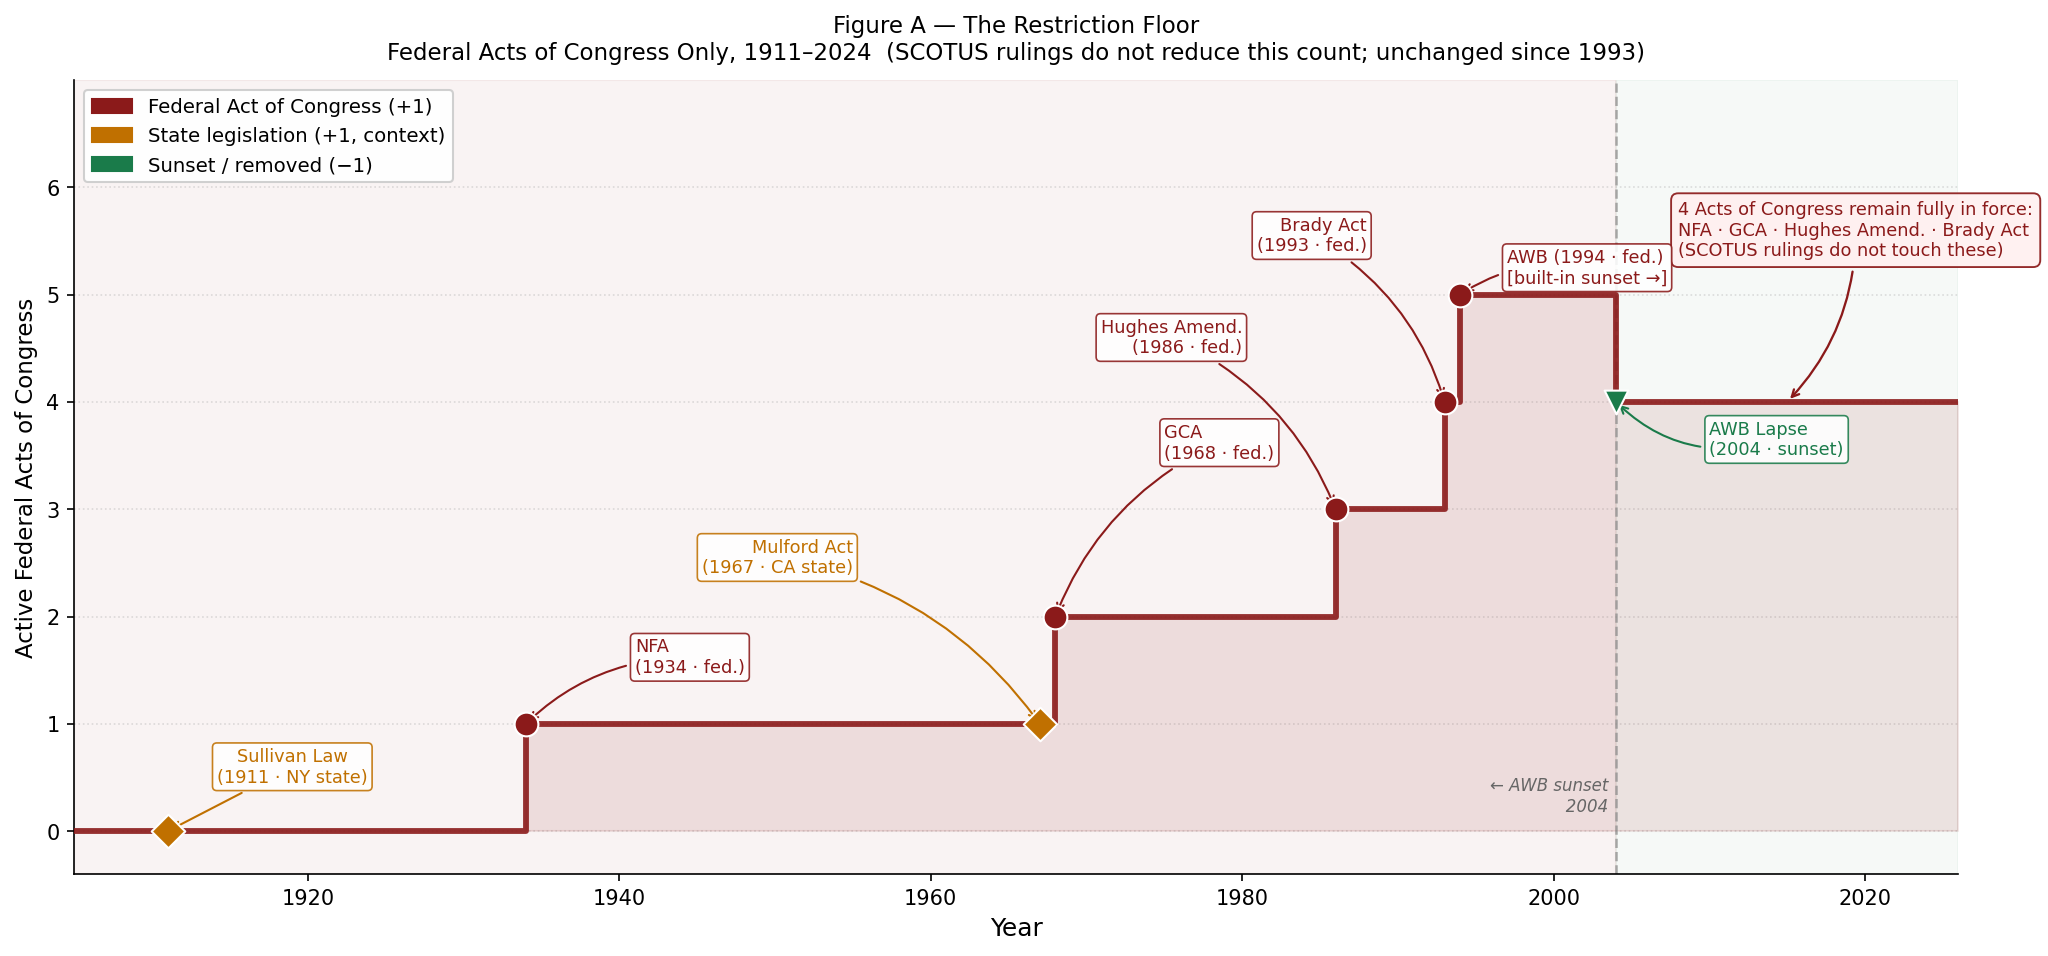
\includegraphics[width=\textwidth]{figures/eq65_68_fig_a_legislation.png}
  \caption{Eq.~65--68 \textbf{(Figure A)}: The Restriction Floor --- Federal Acts of Congress Only, 1911--2024. Active Acts of Congress accumulate from 0 to 5 across 1934--1994 (NFA, GCA, Hughes Amendment, Brady Act, AWB), then drop to 4 when the AWB's built-in sunset clause expires in 2004 --- the NFA, GCA, Hughes Amendment, and Brady Act remain fully in effect regardless of any SCOTUS ruling. State legislation (diamond markers, amber) is shown for context; it does not change the federal count. The flat line at $n=4$ from 2004 to the present represents the durable restriction floor: an Acts of Congress ledge that no rights-expanding SCOTUS ruling has reduced.}
  \label{fig:eq65_68_fig_a}
\end{figure}

\begin{figure}[htbp]
  \centering
  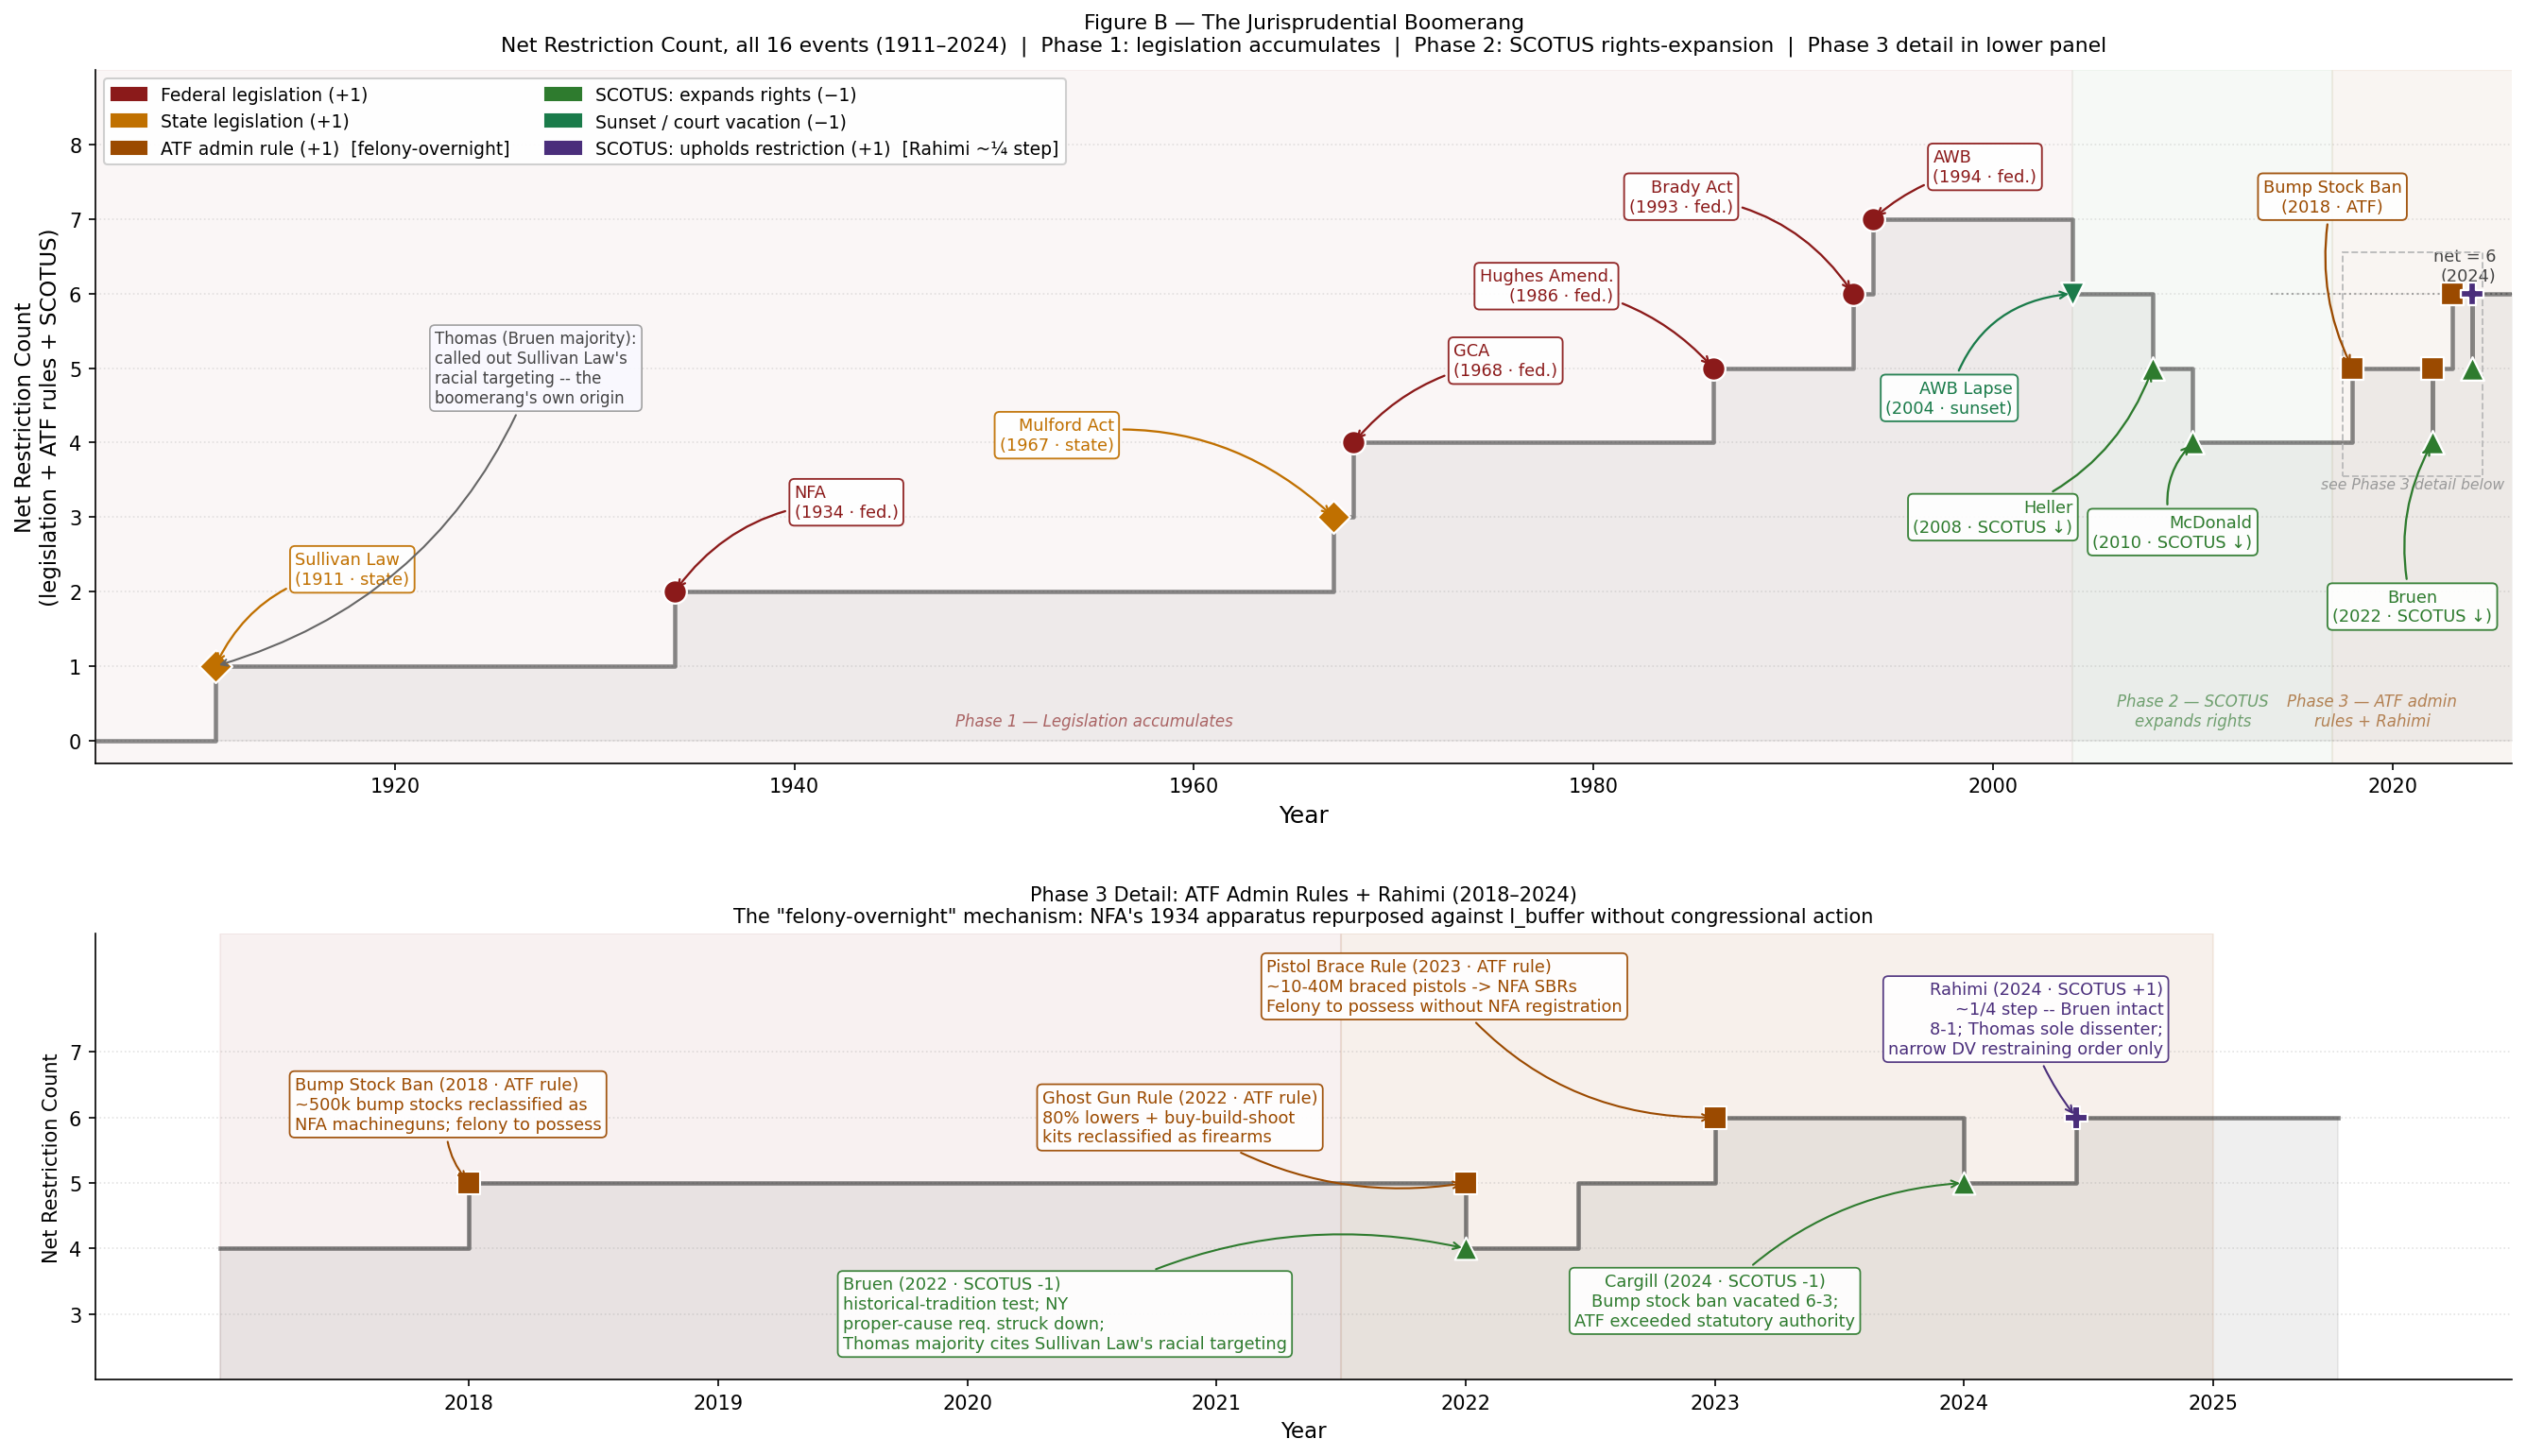
\includegraphics[width=\textwidth]{figures/eq65_68_fig_b_net_restriction.png}
  \caption{Eq.~65--68 \textbf{(Figure B)}: The Jurisprudential Boomerang --- Net Restriction Count Across All 16 Events (1911--2024). \textit{Top panel}: Three-phase arc. Phase~1 (legislation): net rises from 0 to 7 by 1994. Phase~2 (SCOTUS rights-expansion): \textit{Heller}, \textit{McDonald}, and \textit{Bruen} drive the net down to 4 by striking specific state and local restrictions; the federal Acts of Congress floor is untouched. Phase~3 detail is in the lower panel. \textit{Bottom panel}: ATF administrative rule detail, 2018--2024. The \textit{felony-overnight mechanism}: the bump stock ban (2018), ghost gun / frame-receiver rule (2022), and pistol brace rule (2023) are ATF administrative actions that instantly reclassified previously legal property as federal felonies for millions of $I_{\text{buffer}}$ gun owners without a single congressional vote --- deploying the NFA's 1934 administrative apparatus against the population it was not built to manage. \textit{Garland v.\ Cargill} (2024, 6--3) vacated the bump stock ban ($-1$); \textit{United States v.\ Rahimi} (2024, 8--1, $+1$) upheld the domestic violence restraining order gun ban --- a narrow quarter-step: Chief Justice Roberts explicitly reaffirms \textit{Bruen}; Justice Thomas (the \textit{Bruen} author) is the sole dissenter. Terminal net restriction count: 6.}
  \label{fig:eq65_68_2a_case_law}
\end{figure}

\paragraph{Comparison to prediction.}
Equations~\ref{eq:11.1-extraction-precondition}--\ref{eq:11.4-restriction-scope-expansion} predict a four-part sequence: (1) extraction requires Elite lethal dominance over $O_{\text{racialized}}$; (2) the disarmament agenda proceeds as a chronological path; (3) restriction precedents accumulate in doctrine; (4) scope expands from $O_{\text{racialized}}$ to $O_{\text{racialized}} \cup I_{\text{buffer}}$. The data confirm all four predictions with the following precision.

The Sullivan Law, NFA, and Mulford Act are the clearest racial-targeting instances (Phase~1). The Hughes Amendment, Brady Act, and AWB represent the boomerang's mid-arc --- framed as public-safety legislation but deploying the doctrinal apparatus built on racial targeting (Phase~1 to 2 transition). \textit{Heller}, \textit{McDonald}, and \textit{Bruen} are correctly classified as \textit{rights-expanding} events on the agenda path --- they belong in eq:66 but reduce, not add to, the net restriction count. Notably, Justice Thomas's \textit{Bruen} majority opinion explicitly cited the Sullivan Law and historically racially targeted gun laws as the reason the historical-tradition test matters: an anti-racist reading of the same legal doctrine.

The boomerang's sharpest modern arc is the \textit{ATF administrative rule mechanism}. The bump stock ban (2018), ghost gun/frame-receiver rule (2022), and pistol brace rule (2023) are the clearest examples of eq:68's target expansion completing its cycle: the NFA's administrative apparatus --- constructed in 1934 to manage $O_{\text{racialized}}$ under a racial exclusion logic --- is redeployed by executive agencies to instantly reclassify millions of $I_{\text{buffer}}$ gun owners as federal felons without any Act of Congress. The ``felony-overnight'' mechanism is a direct prediction of the framework: once the doctrinal apparatus is entrenched, it can be turned inward.

\textit{Rahimi} (2024) is a quarter step in the same direction but requires precision: \textit{Rahimi} does not overturn or modify \textit{Bruen}. The majority (8--1) explicitly reaffirmed the historical-tradition test; Thomas (the \textit{Bruen} author) was the sole dissenter. The holding is narrow --- adjudicated-dangerous-person with a civil DV restraining order only. Multiple law review analyses characterize \textit{Rahimi} as reinforcing \textit{Bruen}, not retreating from it. The more significant boomerang event in \textit{Bruen}'s wake is not \textit{Rahimi} but the ATF administrative rule campaign that was already underway (2022--2023) using the executive apparatus to outmaneuver a doctrine the $I_{\text{buffer}}$ had just won in court.

\paragraph{Falsification criteria.}
These equations would be falsified if: (1) the federal legislation restriction floor showed a permanent decline via congressional repeal of NFA, GCA, Hughes Amendment, or Brady Act (not a court vacation of an ATF rule, which does not repeal the underlying statute); (2) no restriction-adding event with documented initial $O_{\text{racialized}}$ targeting was later applied to $I_{\text{buffer}}$; (3) the ATF administrative rule mechanism produced no restrictions on $I_{\text{buffer}}$ without congressional action; or (4) the \textit{Bruen} historical-tradition test was applied in a manner that consistently expanded rights without ever upholding restrictions.

Rights-expanding SCOTUS rulings (\textit{Heller}/\textit{McDonald}/\textit{Bruen}/\textit{Cargill}) are the strongest apparent falsification test --- they demonstrate the $I_{\text{buffer}}$ can win legal victories. Yet: (a) not one of these rulings reduced the Acts of Congress restriction floor (NFA, GCA, Hughes, Brady all remain); (b) the ATF responded to \textit{Bruen} (June 2022) with the ghost gun rule (August 2022) and pistol brace rule (January 2023), demonstrating the executive apparatus bypasses SCOTUS victories in real time; (c) the \textit{Bruen} doctrine was applied in \textit{Rahimi} (a quarter step, but directionally consistent with the boomerang). The federal legislation floor has not been touched in 32 years. The boomerang is not a simple accumulation --- it is an adaptive mechanism that routes around I$_{\text{buffer}}$ legal victories through the executive apparatus when the judicial path is temporarily closed.

\paragraph{Confidence tier.}
\textbf{Tier~1.} Primary-source legislation, ATF administrative rules (Federal Register), and Supreme Court rulings with documented legislative and rulemaking history, and peer-reviewed secondary scholarship (Winkler 2011; Cottrol \& Diamond 1991; Harvard JLPP 2024; Virginia Law Review 2024). Sixteen events spanning 113 years provide a robust time-series for all four equations. The racial targeting of the Sullivan Law and Mulford Act is documented in primary-source contemporaneous press coverage and legislative record, not inferred from downstream effects. The ATF administrative rule data (affected population estimates, rulemaking docket numbers, court vacation orders) are drawn from official ATF Federal Register filings and federal court records.

\section{The Rhetorical Bridge: Why This Chapter Exists}

This chapter has traced a continuous thread from Portuguese firearms on the West African coast to the post-Bruen legislative scramble in American state capitals. The thread is a single variable: the Elite's management of lethal asymmetry. The interface changes---from direct military conquest, to constitutional exclusion, to economic filters, to bureaucratic gatekeeping, to grandfather clauses---but the kernel function is constant: maintain $L_E \gg L_O$.

There is a strategic reason this chapter exists in this book, and the framework's commitment to intellectual honesty requires stating it explicitly.

Gun control is the most effective entry point for communicating this framework to the armed Buffer Class.

The Buffer Class gun community is currently experiencing what this book has documented as the cannibalization phase (Section~6.12). The apparatus that was built to disarm $O_{\text{racialized}}$---the economic filters, the bureaucratic friction, the spatial proxy, the grandfather clause---is now being turned on the Buffer Class itself. The suburban gun owner in Massachusetts who had his firearms retroactively reclassified; the rural hunter in New York whose standard-capacity magazines became contraband overnight; the veteran in California navigating an ever-expanding web of registration requirements---each of these individuals is experiencing the extraction algorithm's expansion beyond its original target set.

Add to that list a Virginia licensed-carrier named Ava Marie Gardner. Forced off a highway by a violent aggressor, she drew her firearm, stopped the threat, and fired no shot. The police who arrived arrested her---not the man who had forced her off the road and then advanced on her---because she had crossed into Maryland without a Maryland-specific credential. She was convicted. The Supreme Court denied her petition for review without comment (Section~\ref{subsec:gardner_proof}). Place her case beside Dexter Taylor's: one Black man, one white woman, one temporal retroactive proxy, one geographic retroactive proxy, the same algorithm, the same output function, the same silence from the Court. The framework does not need to predict the Gardner case. The Gardner case confirms the framework's prior prediction---that the spatial proxy architecture constructed on Sullivan Law and Mulford precedent would eventually consume a member of $I_{\text{buffer}}$ who had done everything right. That prediction has now been empirically confirmed in a Maryland traffic stop, a conviction, and a one-line docket entry at One First Street.

When you explain the history of gun control as a pillar of systemic racism---when you show that the NFA was the wages of whiteness applied to firearms, that the Mulford Act was the system panicking because Black people exercised the same rights the Buffer Class takes for granted, that the Hughes Amendment was an economic caste system designed to keep military hardware in the hands of the wealthy---the Buffer Class gun owner recognizes their own experience in the framework. They are living the pattern this chapter documents. The apparatus that was built to extract from $O_{\text{racialized}}$ has expanded to extract from them.

Remember the wages of whiteness from Chapter~\ref{ch:bacon}? The psychological wage that the Elite offered the white working class in exchange for surrendering material solidarity with the racialized Out-group? The Buffer Class gun community is discovering what the framework predicted: the psychological wage was always a loan, and the interest is coming due. The rights they surrendered on behalf of the designated Other are now being surrendered on their behalf.

This is the cross-racial solidarity vector the framework identifies: the moment when $I_{\text{buffer}}$ recognizes that their material interests have always aligned with $O_{\text{racialized}}$ rather than with $E$. The kinetic guarantee is the common ground---the single issue where the Buffer Class and the Out-group share an existential interest in resisting the Elite's containment architecture. When a Black gun owner in Oakland and a white gun owner in rural Massachusetts both understand that the system taking their firearms is the same system, operating through the same algorithm, serving the same Elite---the partition that has kept them separated for three centuries begins to dissolve.

The framework makes no prediction about whether this solidarity will materialize. It merely observes that the mathematical conditions for it have never been more favorable, and that the disarmament timeline is the thread that makes the common interest visible.

\part{Diagnostics and Output}
\label{part:diagnostics}

\chapter{The Contradiction: Why Reform Serves the Algorithm}
\label{ch:contradiction}

\begin{tcolorbox}[colback=black!5, colframe=black!70, fonttitle=\bfseries\ttfamily, title=RUNTIME LOG: TESTING PRESCRIPTIVE INTERVENTIONS AGAINST KERNEL LOGIC]
\ttfamily\small
\textbf{System Stress} ($\min$: class resistance): \textcolor{red}{\textbf{FAILING}} --- $I_{\text{buffer}}$ awakening to contract breach. Kinetic capacity of civilian population exceeds $F_{\text{enforce}}$. Cross-racial solidarity vectors reappearing.\\
\textbf{Capital} ($\max$: extraction output): TERMINAL PHASE --- Extraction zone expanded beyond $O$ into $I_{\text{buffer}}$. Opioid crisis{,} affordability trap{,} and universal latent criminality consuming the system's own defenders.\\
\textbf{Interference State} ($\Phi_{\text{load}}$, proximity to $\tau$): SATURATED BUT SLIPPING --- maximum phase-loading encountering diminishing suppression returns. Estimated $\Phi_{\text{load}} \in [0.82, 0.95]$, $\rho_{\tau} \in [0.92, 1.05]$.\\
\textbf{Variables Loaded}: Full 5-tier hierarchy + all proxy variables.\\
\textbf{Executing Function}: Algorithm fully mapped. Switching from diagnostic to prescriptive mode.\\
\textbf{CRITICAL WARNING}: Prescriptive interventions must be stress-tested against the kernel's own optimization logic. A ``solution'' that reduces $\min$ (class resistance) without dismantling $\max$ (extraction capacity) is not a solution---it is \textbf{maintenance}.
\end{tcolorbox}

\medskip

The preceding chapters have traced an unbroken algorithmic thread: from the Portuguese invention of racial hierarchy, through the constitutional embedding of extraction via the 13th Amendment, to the modern deployment of proxy variables that now cannibalize the very Buffer Class the system created to protect itself. Each phase of the Elite's optimization reveals a system that adapts its \textit{interface} while preserving its \textit{kernel}: the Predatory Min-Max Function that maximizes extraction while minimizing class resistance.

If this diagnostic is correct, it constrains the space of effective prescriptions. Interventions that target only the system's \textit{interface}---its current legal language, its present-day proxies---will be absorbed and neutralized, as every previous reform movement has been. Effective policy must target the kernel itself: the Predatory Min-Max Function and the economic architecture that sustains it. But here the framework confronts its own most devastating implication: \textit{the system is designed to offer precisely these reforms when its survival requires them}.

In virus terms, this chapter asks whether the proposed cure patches the payload or merely reduces symptoms enough for the host to keep running. A reform that makes the infected system feel less cruel while leaving the extraction kernel intact is not an uninstall routine. It is palliative maintenance for the host wetware, preserving legitimacy long enough for the virus to recompile around the patch.

\section{The Reform Paradox: Why Policy Audits Serve \texorpdfstring{$\min$}{min}}

The mathematical framework reveals a fundamental shift from individual-focused solutions to systemic policy reform. Consider a concrete scenario: a bank deploys a machine-learning model for loan approvals. The algorithm uses features including zip code, employment-gap history, and credit score. No feature explicitly references race. Yet because redlining ($P_{\text{redlining}}$) concentrated $O_{\text{racialized}}$ into specific zip codes, and because the War on Drugs ($P_{\text{WarOnDrugs}}$) created disproportionate employment gaps through incarceration, these ``neutral'' features encode the full compounding chain of Section~4.5. The zip-code variable is not a proxy for race---it is a \textit{fossil record} of $O_{\text{racialized}} \cap P_{\text{redlining}}$, and the employment-gap filter is a fossil record of $O_{\text{racialized}} \cap P_{\text{WarOnDrugs}}$.

The critical insight is this: \textit{you stop looking for the bad actor and start looking for the disproportionate intersection}. The loan officers may harbor zero racial animus. The engineers who built the model may have the best of intentions. The disparity persists because the policy $P_{\text{algorithm}}$ structurally intersects with $O_{\text{racialized}}$ through historically encoded features. The framework demands an audit of the intersection $O_{\text{racialized}} \cap P$ and the direct modification of $P$ to reduce it:

\medskip
\noindent
\begin{tabular}{@{}p{0.47\textwidth}|p{0.47\textwidth}@{}}
\textbf{Traditional (Individual-Focused)} & \textbf{Framework (Intersection-Focused)} \\
\hline
Sensitivity training for loan officers & Audit algorithm parameters for $O_{\text{racialized}} \cap P$ \\[4pt]
Implicit bias workshops for staff & Identify features that encode historical policy (zip code $\leftarrow P_{\text{redlining}}$, employment gaps $\leftarrow P_{\text{WarOnDrugs}}$) \\[4pt]
Diversity hiring in the lending department & Remove or reweight biased features; validate that $|O_{\text{racialized}} \cap P'| < |O_{\text{racialized}} \cap P|$ \\[4pt]
Individual complaint mechanisms & Continuous structural monitoring: measure the intersection after every model update \\[4pt]
\textit{Result}: Algorithm unchanged $\rightarrow$ disparity persists & \textit{Result}: Algorithm restructured $\rightarrow$ disparity structurally reduced \\
\end{tabular}

\medskip
This intersection-focused approach is mathematically superior to individual-focused solutions, which the framework makes \textit{predictable failures}. If the policy $P$ structurally targets the Out-group---if $|O_{\text{racialized}} \cap P| \gg |I \cap P|$ by design---then modifying individual behavior within that system cannot eliminate the disparity. The inequality is built into the policy's structure. The analytical focus must shift from ``Do individual actors harbor bias?'' to ``Is this policy $P$ inherently unequal in its design?''

This analytical approach applies to any domain where racial disparities exist: criminal `injustice' (audit stop-and-frisk, mandatory minimums), education (audit funding formulas, attendance boundaries), employment (audit job requirements, salary structures). By mathematically identifying $O_{\text{racialized}} \cap P$ as the site of harm, the framework makes policy reform non-negotiable for anyone who accepts the model's premises.

\medskip
\textbf{The Paradox}

\medskip
And here is the contradiction that the framework cannot escape. Every one of these reforms---auditing the lending algorithm, reweighting the zip-code variable, reducing the intersection $|O_{\text{racialized}} \cap P|$---\textit{directly serves the $\min$ variable of the Predatory Min-Max Function}.

Recall the function's architecture: $E$ simultaneously maximizes extraction ($\max$) and minimizes class resistance ($\min$). A policy reform that marginally reduces the Out-group's suffering does not touch $\max$; it reduces $\min$. It bleeds off precisely enough pressure to prevent the system from reaching kinetic threshold. Formally:
\begin{equation}\label{eq:12.1-reform-absorption-mechanism}
\min(t+1) = \min(t) - \epsilon \cdot \Delta|O_{\text{racialized}} \cap P'|
\end{equation}
where $\epsilon$ represents the marginal reduction in class resistance produced by the reform.\footnote{This equation is classified as Tier~3 (ordinal/structural); the structural reform-absorption mechanism is validated by the six-case Concession Theorem evidence in $\S$\ref{sec:concession_theorem}, each of which demonstrates that policy reform reduces $\min$ (class resistance) without altering $\max$ (Elite extraction share), consistent with $\Delta\max = 0$. See the Empirical Methodology chapter (p.~\pageref{ch:empirical_methodology}) and Appendix~\ref{app:empirical_index}.} Each successful policy audit \textit{extends the algorithm's operational lifespan} by lowering the probability that the exploited population reaches the threshold of coordinated kinetic resistance.

This is not speculation. It is the historical record of the manuscript itself. It is also not an informal observation: in the formal containment model of Section~\ref{sec:formal-containment-model}, the closed-loop system admits a Lyapunov function $V(q)$ with $\dot V(q) \leq 0$ along every trajectory (Theorem~\ref{thm:integer-convergence}, \cite{khalil_nonlinear, kan_containment}). $V$ is the ``volume of freedom''---the measure of the portion of state space the population can reach under its own dynamics. The theorem states that this volume is \textit{monotonically non-increasing}. A policy audit that reduces $|O_{\text{racialized}} \cap P|$ is a perturbation which the closed-loop control law re-absorbs into a descent direction of $V$: the reform is not outside the algorithm's invariant set; it is one of the directions in which the algorithm was already constructed to move. This is the Lyapunov-theoretic statement of what the chapters that follow demonstrate as historical fact.

\section{The Concession Theorem: Historical Proof}
\label{sec:concession_theorem}

The framework's own evidence, traced across five centuries, demonstrates that every major non-kinetic reform in the American dataset was deployed---or permitted---by the Elite ($E$) at the precise moment when the $\min$ variable approached failure:

\begin{enumerate}
    \item \textbf{The Wages of Whiteness (1705):} Following Bacon's Rebellion (1676), which represented a catastrophic $\min$ failure---cross-racial solidarity among the laboring class---the Elite did not crush the rebellion and restore the prior system. They \textit{reformed} it. The Virginia Slave Codes granted psychological wages ($\psi$) to the white working class, partitioning the labor force and resetting $\min$ to a stable equilibrium. The reform was the patch.

    \item \textbf{The Emancipation Proclamation (1863):} Lincoln's executive order was not a moral epiphany; it was a military strategy to destabilize the Confederacy's labor base. As Du Bois documented, the Out-group had already forced the military equation: the general strike of approximately 500,000 self-emancipating enslaved people (Section~\ref{sec:general_strike_sub}) had collapsed the Confederacy's logistical foundation before Lincoln's executive order \cite{dubois}. The ``liberation'' was the Union government's institutional recognition of a fait accompli produced by $O_{\text{racialized}}$ kinetic action. The 13th Amendment then immediately re-encoded extraction through its exception clause---the kernel recompiled around the reform.

    \item \textbf{Reconstruction and Its Counter-Revolution (1865--1877):} The period immediately following the 13th Amendment produced the most complete multiracial democratic experiment in American history. Reconstruction governments---built on a coalition of freedmen, free Black Northerners, and white Southern Unionists---established public education systems for both races, expanded labor rights, passed civil rights legislation, and elected Black representatives to Congress and state legislatures at levels not replicated for a century. The $\min$ variable registered its lowest value in American history; the Out-group possessed electoral power, institutional presence, and incipient land claims.

    Du Bois's analysis in \textit{Black Reconstruction} \cite{dubois} is definitive: the counter-revolution that ended Reconstruction was not driven primarily by Southern racism but by a \textit{class alliance}---Northern industrial capital and Southern Redeemer elites recognizing that multiracial democracy threatened extraction at the national scale. The Freedmen's Bureau land redistribution program (40 acres) would have created an independent Black landowning class outside the extractive agricultural system. The Reconstruction labor laws threatened to raise wages for both Black and white workers by creating competitive bidding for labor in the South. The Elite's response was to fund, coordinate, and legitimize the Redeemer campaign---combining paramilitary violence (the Ku Klux Klan, the Red Shirts) with electoral fraud and the withdrawal of federal enforcement. The Compromise of 1877 formalized the deal: Northern capital removed federal troops from the South, handing Reconstruction's multiracial democracy to Redeemer violence, in exchange for the railroad land grants and tariff protections that would fund industrial expansion. $\Delta\max = 0$: the reforms were permitted just long enough to stabilize the post-war $\min$ threshold, then dismantled the moment the kinetic threat subsided.

    \item \textbf{The New Deal (1933--1944):} The Great Depression produced the most severe $\min$ failure in American history---mass unemployment, the Bonus Army encampment in Washington, surging Communist Party membership, Huey Long's radical wealth-redistribution coalition threatening Roosevelt's left flank. Status wages alone ($\psi_s$) could not hold $M(t)$ below $\tau$. The Elite escalated to the material wage ($\psi_m > 0$): Social Security, the GI Bill, FHA-subsidized homeownership, and federally protected collective bargaining. These were real, generation-defining material benefits---the foundations of the American white middle class.

    The mechanism of sourcing is the theorem's proof. Every pillar of the New Deal's material wage was built on the explicit exclusion of $O_{\text{racialized}}$. The Social Security Act (1935), the National Labor Relations Act (1935), and the Fair Labor Standards Act (1938) all excluded agricultural workers and domestic servants---the two occupational categories employing approximately 65\% of Black workers---at the explicit demand of Southern Democrats protecting the plantation economy \cite{katznelson_fear}. The GI Bill's administration was decentralized to local officials: in Mississippi in 1947, 3,229 federally guaranteed home loans were issued; two went to Black veterans \cite{katznelson_fear}. The FHA (1934) institutionalized redlining, and between 1934 and 1962, only 2\% of \$120 billion in federally subsidized new housing reached non-white families. The New Deal was not a race-neutral recovery program with unfortunate gaps; it was a \textit{racially partitioned material wage}: $\psi_m$ deployed to $I_{\text{buffer}}$, funded by stripping $O_{\text{racialized}}$ of access to the same programs and deepening their spatial and economic enclosure through FHA-mandated segregation. $\Delta\max = 0$ for $E$. The Great Compression was a white compression.

    The theorem's temporal prediction was also confirmed: once the kinetic threat of the Depression era subsided, the material wage was gradually clawed back. By 2020, wealth concentration had returned to 1920s Gilded Age levels. The kernel recompiled.

    \item \textbf{The Civil Rights Act (1964):} The legislation followed a decade of kinetic urban revolt---Birmingham, the Freedom Rides, Watts. The $\min$ variable was failing catastrophically. The Elite permitted the interface update (desegregation, voting rights) while simultaneously preparing the Variable Swap (the War on Drugs) that would preserve the extraction kernel under race-neutral language. The reform was the interface swap's cover story.

    \item \textbf{The Fair Sentencing Act (2010):} Congress reduced the crack-to-powder cocaine sentencing ratio from 100:1 to 18:1---an explicit acknowledgment that the original ratio was unjust. Yet the Act provided \textit{no retroactive relief}, leaving tens of thousands of Black citizens to serve out sentences that Congress itself had declared disproportionate. The system updated its interface while leaving the existing extraction intact. $\min$ was reduced; $\max$ was untouched.

    \item \textbf{Women's Suffrage and Labor Force Entry (1920--1970s):} The Nineteenth Amendment and the subsequent mass entry of women into the formal labor market is perhaps the most structurally elegant demonstration that the Concession Theorem operates across \textit{every} axis of the extraction architecture, not only the racial one. The ``liberation'' doubled the available labor supply. Elementary price theory dictates what followed: when the supply of a commodity doubles against relatively inelastic demand, its unit price collapses. Real wages per worker stagnated and then declined, and by the late twentieth century a household required two full-time incomes to approximate the purchasing power that a single income had provided a generation earlier. The Elite's extraction rate ($\max$) did not merely survive the reform---it \textit{increased}, because the same household now fed twice the labor hours into the production function while the surplus flowed upward through the same capital ownership structures.

    Critically, the societal expectations encoded by the ``divine sphere'' ideology documented in Chapter~\ref{ch:gendered} were never repealed. Men remained the culturally designated providers; women remained the culturally designated domestic laborers. The reform \textit{added} a second shift to women's load without subtracting the first. For Black women---who had never been afforded the ``protection'' of the domestic sphere and had been subjected to compulsory labor extraction since 1619---the compounding was doubly devastating: they absorbed the racial extraction ($O_{\text{racialized}} \cap P$) \textit{and} the gendered wage depression simultaneously, with no corresponding reduction in either the domestic burden or the carceral targeting documented in Chapter~\ref{ch:recompile}. The ``concession'' of formal labor equality thus functioned as a supply-side subsidy to $E$: it halved the unit cost of labor, doubled household dependency on wage income, and left the extraction kernel not only intact but operating at higher throughput.
\end{enumerate}

\subsection{The Durability Objection: When Reforms Appear to Persist}

Before formalizing the theorem, the framework must answer the objection that a careful critic will immediately raise: some reforms appear durable. The Occupational Safety and Health Act (1970) reduced industrial fatality rates by roughly 65\% over five decades and has not been substantively repealed. The 40-hour workweek, established by the Fair Labor Standards Act (1938), remains legally operative. Post-1965 Black voter registration in the Deep South rose from under 30\% to near-parity and, while periodically suppressed, has not returned to pre-Civil Rights levels. If the Concession Theorem predicts that every reform is absorbed without residue, these cases constitute apparent falsifications.

The theorem withstands the objection through a two-part diagnostic test that any claimed counter-example must satisfy before it qualifies as a genuine falsification.

\textbf{Part I: Was the gain eventually clawed back?} The historical record demonstrates that concessions calibrated to suppress kinetic threat are reversed once the threat subsides. The New Deal's material wage (documented above) was clawed back across the following seven decades: union density peaked at 35\% in 1954 and had collapsed to 10\% by 2020; real wages for non-supervisory workers stagnated from 1973 through 2020 while productivity doubled; and by 2020 wealth concentration had returned to 1920s Gilded Age levels. The gains were real in the moment they were granted; they were not permanent. A reform that requires continuous kinetic threat to maintain itself is not evidence of $\Delta\max \neq 0$---it is evidence of the theorem's prediction that concessions track the threat level of $\min$.

\textbf{Part II: If the gain has not been clawed back, does $\Delta\max = 0$ still hold?} This is the subtler and more important test. A reform $R_i$ can produce a persistent, non-reversed reduction in $\min$ (the Out-group or working class retains a measurable gain) without producing $\Delta\max \neq 0$, provided the extraction rate is compensated elsewhere in the production function. Formally, the theorem does not require that $\Delta\min(R_i) = 0$ for every reform; it requires only that:
\[
\Delta\max(R_i) = 0 \quad \text{even when} \quad \Delta\min(R_i) < 0 \text{ persists}
\]
The interface has been updated; the kernel is untouched. OSHA is the clearest illustration: industrial fatality reduction lowered one measure of worker harm, but it simultaneously reduced the liability exposure of $E$, stabilized the labor supply (dead workers do not produce), and was structured to impose compliance costs that fell more heavily on smaller competitors than on large capital---the regulation consolidated $E$'s market position while appearing to constrain it. The 40-hour week created the weekend leisure economy, expanding the consumer surface area that capital extracts from. The reforms were not neutral gifts; they were interface updates that increased the extraction architecture's long-run efficiency.

The aggregate test is the decisive one. If any of these durable reforms had produced $\Delta\max \neq 0$---had structurally reduced the Elite's extraction capacity---the evidence would appear in the long-run wealth concentration data. It does not. By 2020, the top 1\% of American households held approximately 32\% of total net worth, and the top 10\% held 69\%---numbers statistically indistinguishable from the pre-New Deal 1920s, despite intervening decades of labor law, safety regulation, civil rights legislation, and environmental protection. The Concession Theorem does not require that every reform produce zero welfare gain for the Out-group; it requires that the extraction kernel---$\max$ at the apex---remains inviolate across the reform cycle. The data confirms this invariant.

The durability objection, properly analyzed, is not a counter-example to the theorem. It is the theorem's mechanism made visible: the system permits reforms that stabilize the Out-group's participation in the production function \textit{because} those reforms extend the algorithm's operational lifespan. A reform durable enough to become structurally embedded is durable precisely because it serves $\min$-management efficiently.

The pattern is mathematically unambiguous. We can formalize it as the \textbf{Concession Theorem}:

\begin{definition}[The Concession Theorem]
The Elite ($E$) will permit or initiate policy reforms at a rate proportional to the threat level of $\min$---offering concessions \textit{just sufficient} to prevent the kinetic threshold from being crossed, but \textit{never sufficient} to alter the extraction kernel ($\max$). Formally:
\begin{equation}\label{eq:12.2-concession-theorem}
\text{Reform Rate}(t) \propto \frac{d(\min)}{dt} \quad \text{subject to} \quad \Delta\max = 0
\end{equation}
The constraint $\Delta\max = 0$ is the invariant: no reform in the historical dataset has ever reduced the Elite's extraction capacity. Every concession was calibrated to reset $\min$ without touching $\max$.
\end{definition}

\noindent\textit{Tier~2 Illustrative Instantiation --- New Deal as Anchor Case.} The New Deal (1933--1944) is the theorem's strongest single-event test. The Great Depression produced catastrophic $\min$ failure: Bonus Army encampment in Washington (1932), Communist Party membership surging from 7,500 to 55,000 members (1930--1938), and Huey Long's wealth-redistribution coalition threatening Roosevelt's left flank---precisely the kinetic-threat conditions the theorem predicts drive concession deployment. The reform rate $\propto d(\min)/dt$ was maximal. $E$ deployed $\psi_m > 0$: Social Security, GI Bill, FHA homeownership, and federally protected collective bargaining were real, generation-defining benefits. But the $\Delta\max = 0$ constraint held through the sourcing mechanism: every pillar excluded approximately 65\% of Black workers (agricultural and domestic exemptions at Southern Democratic demand \cite{katznelson_fear}). Piketty-Saez-Zucman DINA data \cite{piketty_saez_zucman_2018} show top 10\% wealth share falling from $\approx$85\% (1929) to $\approx$64\% (1978) and recovering to $\approx$70\% by 2020---confirming $\Delta\max = 0$ across the full reform cycle: the Great Compression was real, but transient. The reform rate tracked the threat gradient: the New Deal was preceded by the Bonus Army, Communist Party surge, and Huey Long coalition; the Civil Rights Act (1964) was preceded by Birmingham, Freedom Rides, and Watts. Once $\min$ stabilized, the material wage was clawed back. Confidence: Tier~2; Piketty-Saez-Zucman wealth share data are Tier~1; the causal claim that reform rate tracks $\min$-threat is a structural interpretation \cite{piven_cloward_1977}.

\begin{figure}[htbp]
\centering
\begin{tikzpicture}
\begin{axis}[
    width=13cm, height=6.5cm,
    xlabel={Year},
    ylabel={Top 10\% Wealth Share (\%)},
    xmin=1910, xmax=2025,
    ymin=55, ymax=92,
    xtick={1920,1933,1945,1964,1978,1981,2001,2008,2020},
    xticklabels={1920,1933,1945,1964,1978,1981,2001,2008,2020},
    x tick label style={rotate=45, anchor=east, font=\footnotesize},
    y tick label style={font=\footnotesize},
    grid=major,
    grid style={dashed, gray!30},
    axis lines=left,
    tick align=outside,
    legend pos=south east,
    legend style={font=\tiny},
]

% Wealth share trajectory (Piketty--Saez--Zucman, WID.world)
\addplot[thick, black, mark=*, mark size=1.5pt] coordinates {
    (1913, 80)
    (1920, 82)
    (1929, 85)
    (1933, 83)
    (1945, 69)
    (1953, 65)
    (1965, 64)
    (1978, 64)
    (1983, 66)
    (1990, 68)
    (2000, 72)
    (2007, 75)
    (2010, 74)
    (2020, 70)
};
\addlegendentry{Top 10\% wealth share}

% Reference band: pre-New Deal baseline (1913--1933 average ~82%)
\addplot[dashed, gray!60, thick] coordinates {(1910,82)(2025,82)};
\addlegendentry{Pre-New Deal baseline ($\approx$82\%)}

% Reform event annotations -- vertical dashed lines
\draw[dashed, red!60, thin] (axis cs:1933,55) -- (axis cs:1933,92);
\draw[dashed, blue!50, thin] (axis cs:1964,55) -- (axis cs:1964,92);
\draw[dashed, orange!70, thin] (axis cs:1981,55) -- (axis cs:1981,92);
\draw[dashed, purple!50, thin] (axis cs:2001,55) -- (axis cs:2001,92);
\draw[dashed, brown!60, thin] (axis cs:2008,55) -- (axis cs:2008,92);

% Event labels at top of figure
\node[rotate=90, anchor=south west, font=\tiny, text=red!70] at (axis cs:1933,85) {New Deal (1933)};
\node[rotate=90, anchor=south west, font=\tiny, text=blue!70] at (axis cs:1964,85) {Civil Rights (1964)};
\node[rotate=90, anchor=south west, font=\tiny, text=orange!80] at (axis cs:1981,85) {Reagan cuts (1981)};
\node[rotate=90, anchor=south west, font=\tiny, text=purple!70] at (axis cs:2001,85) {Bush cuts (2001)};
\node[rotate=90, anchor=south west, font=\tiny, text=brown!70] at (axis cs:2008,85) {Crisis (2008)};

% Delta-max label
\node[anchor=west, font=\footnotesize\itshape, text=black] at (axis cs:1913,57) {$\Delta\max = 0$ invariant: kernel share returns to baseline across all reform cycles};

\end{axis}
\end{tikzpicture}
\caption{\textbf{The $\Delta\max = 0$ Invariant: Top 10\% Wealth Share, 1913--2020.} Despite the New Deal, the Civil Rights Act, environmental and labor legislation, and multiple rounds of progressive tax reform, the Elite's aggregate extraction share---measured as the top decile's portion of total national wealth---returns to near its pre-New Deal baseline by 2020. Each major reform cycle (annotated) produced a temporary downward perturbation, but the closed-loop system re-absorbed every reform and the wealth share resumed its long-run trajectory. This is $\Delta\max = 0$ stated as an empirical time series: the extraction kernel is invariant across every concession in the 1913--2020 dataset. Data from Piketty, Saez, and Zucman (WID.world).}
\label{fig:deltamax_invariant}
\end{figure}

\subsection{The Extraction Engine: Why \texorpdfstring{$\Delta\max = 0$}{Δmax = 0} Is a Legal Mandate}

The Concession Theorem's invariant---$\Delta\max = 0$---is not merely an empirical observation drawn from the historical record. It is \textbf{structurally encoded into the legal architecture of the corporation itself}.

Under the doctrine of \textbf{shareholder primacy}, corporate officers bear a fiduciary duty to maximize returns to shareholders. This is the extraction kernel expressed as corporate law: the entity that \textit{directly produces} the capital---the corporation---is \textit{legally obligated} to maximize its extraction rate. A CEO who voluntarily reduces profit margins to improve labor conditions or community welfare risks shareholder derivative suits, hostile board action, and termination. The Predatory Min-Max Function is not a metaphor at the corporate level; it is the \textbf{job description}.

The incentive architecture ensures that the individuals managing the extraction engines are personally fused to the extraction rate. Executive compensation in the modern era is overwhelmingly denominated not in cash salary but in \textbf{equity}: stock options, restricted stock units, and performance shares whose value is a direct function of the firm's market capitalization. The CEO's personal wealth \textit{is} the extraction output. Their net worth does not merely correlate with $\max$; it is $\max$, measured in real time on a ticker. Every structural decision---wage suppression, offshoring, algorithmic labor scheduling, union avoidance---that increases the firm's equity price simultaneously increases the executive's personal fortune. The alignment is total: the human being operating the extraction engine is compensated in units of extraction.

The final architectural layer is the mechanism by which this extracted wealth is \textit{consumed without ever being taxed}. Under the U.S.\ tax code, unrealized capital gains are not income. A CEO whose equity portfolio appreciates by \$500 million in a single year owes \$0 in taxes on that appreciation---because no ``taxable event'' has occurred. To access the wealth for consumption, the executive does not sell the stock (which would trigger capital gains tax and reduce the equity position). Instead, they execute what tax professionals term the \textbf{Buy-Borrow-Die} strategy: they pledge the appreciated stock as collateral and take out low-interest margin loans against it. The loan proceeds are not taxable income. As long as the portfolio appreciates faster than the loan's interest rate---a condition the extraction engine itself is legally mandated to produce---the executive can take out successive loans indefinitely, rolling the balance forward, consuming unlimited liquidity without ever realizing a taxable gain. Upon death, the assets receive a \textbf{stepped-up basis} under IRC \S 1014, resetting the cost basis to the current market value and permanently erasing the unrealized appreciation from the tax base. The heirs inherit the wealth; the treasury receives nothing; the cycle restarts.

This is the mechanical specification of $\Delta\max = 0$. The corporation is legally required to maximize extraction. The executives are compensated in units of extraction. And the tax architecture permits the extracted wealth to be consumed, inherited, and perpetuated without ever passing through the public treasury. No reform that leaves this trilateral architecture intact---fiduciary duty, equity compensation, and the Buy-Borrow-Die loop---can produce $\Delta\max \neq 0$. The constraint is not a pattern the Elite happens to maintain; it is a \textbf{legal machine} that runs whether any individual Elite member wills it or not.

The Concession Theorem predicts that the policy prescriptions identified in this chapter---algorithmic audits, intersection reduction, structural monitoring---are \textit{exactly} what the system will offer when $\min$ approaches failure in the current terminal phase. The framework that diagnoses the disease also predicts the palliative the system will administer. Accepting these reforms resets the clock.

\subsection{Algorithmic Load Balancing: Freedom as a Zero-Sum Market}

The clock resets because the system does not concede extraction; it reroutes it. Let $\ell_g(t)$ denote the extraction load assigned to demographic or jurisdictional group $g$ at time $t$. The Elite's target is not merely to keep one group subordinate but to maintain the aggregate extraction yield:
\begin{equation}\label{eq:12.2a-load-balancing}
\sum_{g \in G} \ell_g(t) = \mathcal{E}_{\text{total}}(t),
\qquad
\frac{d\mathcal{E}_{\text{total}}}{dt} \geq 0 .
\end{equation}
If a reform reduces the load on one group without altering $\mathcal{E}_{\text{total}}$, the deficit must be assigned somewhere else:
\begin{equation}\label{eq:12.2b-load-transfer}
\Delta \ell_h
=
-\Delta \ell_g
+ \Delta \mathcal{E}_{\text{total}},
\qquad h \neq g .
\end{equation}

This is the mechanical basis of horizontal hostility. The system pitches groups against each other because each partial concession is experienced by another group as a new burden, a lost status wage, a price increase, a tax shock, a policing surge, or a moral panic. The market being rationed is not money alone but freedom itself. One population receives a partial autonomy patch; another population is made to pay for it through deeper extraction or diminished access. The resulting conflict is then misread as cultural antagonism rather than as load balancing by the extraction kernel.

\subsection{The Acemoglu Limit: Why ``Inclusive Institutions'' Cannot Recompile Without Dismantling the Racial Partition}
\label{sec:acemoglu_limit}

Acemoglu and Robinson's \textit{Why Nations Fail} is the most influential contemporary articulation of the institutional-economics theory of extraction \cite{acemoglu_robinson}. Their core argument---that the divergence between prosperous and impoverished nations reduces to the distinction between ``inclusive'' and ``extractive'' institutions, with the latter concentrating political and economic power at the apex and blocking the creative destruction required for long-run growth---correctly identifies the architecture this book has traced for five centuries. Their comparative historical dataset, their identification of ``critical junctures'' at which institutional divergence becomes self-reinforcing, and their analysis of elite capture of political institutions all converge with the framework developed here at the level of description.

The Acemoglu Limit is the point at which their prescription fails. AJR's solution is the construction of ``inclusive institutions''---pluralist political systems, property rights enforced for all citizens, and competitive markets constrained by centralized state authority. The prescription is that if a nation can navigate the transition from extractive to inclusive, the self-reinforcing logic of inclusive institutions will stabilize the outcome. The problem is that this prescription contains no variable for the racial partition, no term for the psychological wage ($\psi$), and no mechanism for the kinetic-guarantee asymmetry. It treats elite capture as a problem of institutional design that can be solved by institutional redesign---by building better rules.

The Concession Theorem falsifies this prescription at every historical juncture. The arc from Reconstruction to the Compromise of 1877 is the purest laboratory case: the United States briefly constructed inclusive institutions during Reconstruction---multiracial legislatures, universal public education, federal civil rights enforcement---and the extraction Elite dismantled them within twelve years, not by violating the institutional rules but by operating through them. The ``inclusive institutions'' were recompiled into extractive ones because the Elite retained three variables that AJR's model cannot account for. First, the psychological wage ($\psi$) caused $I_{\text{buffer}}$ to defect from the cross-racial coalition in exchange for racial status, supplying the political mass needed to legitimize the Redeemer counter-revolution. Second, the racial partition ($I_{\text{buffer}}$ vs.\ $O_{\text{racialized}}$) ensured that the Out-group's democratic gains were politically isolable---the Reconstruction coalition could be severed along the racial seam the Elite had installed in 1705. Third, the kinetic-guarantee asymmetry meant that when federal enforcement was withdrawn, the paramilitary enforcement class ($F_{\text{enforce}}$) could impose Redeemer rule through violence that the disarmed Out-group could not match.

Formally, AJR's model is a special case of the Concession Theorem with $\psi = 0$ and no racial partition installed. In a system where the Elite have not successfully deployed a psychological wage to purchase buffer-class complicity, institutional reform can achieve durable equilibrium because the reforming coalition cannot be ethnically fragmented. The American case---and, as Chapter~\ref{ch:global} demonstrates, the global colonial system---is not that special case. The racial partition is installed. $\psi$ is operative. The kinetic asymmetry is legally maintained. Under these conditions, building ``inclusive institutions'' without first dismantling the extraction kernel's three-variable architecture does not produce inclusive equilibrium; it produces Reconstruction---a brief inclusive episode followed by violent counter-revolution and kernel restoration.

The conclusion is not that AJR are wrong about what causes nations to fail. It is that their model lacks the variables required to write the patch. \textit{Why Nations Fail} diagnoses the disease with considerable precision; it cannot specify the cure because the cure requires the full five-tier framework---including the psychological-wage mechanism, the racial-partition dynamics, and the kinetic-guarantee architecture---that this book has developed. Inclusive institutions are a necessary condition of the post-kinetic republic; they are not sufficient without simultaneous dismantling of the partition that causes inclusive reforms to recompile back into extraction.

\subsubsection{The Non-Atlantic Objection: Botswana, South Korea, and the Reversal of Fortune}

A critic familiar with the breadth of AJR's empirical work will raise the following objection: the Acemoglu Limit is argued here exclusively through Atlantic cases (Reconstruction, the American dataset). But AJR's empirical program extends far beyond the Atlantic. Their 2002 paper ``Reversal of Fortune'' \cite{ajr_reversal} (Acemoglu, Johnson, and Robinson) documents a striking pattern across former European colonies: societies that were \textit{more} urbanized and densely populated before colonization---and thus, by most pre-modern indicators, more institutionally sophisticated---became \textit{less} developed after colonization, while less-developed pre-colonial territories eventually surpassed them. AJR explain this reversal through the \textit{settler mortality} hypothesis: where European settlers could survive (low disease burden), they built inclusive settler institutions; where they could not, they built pure extraction colonies designed to export resources to the metropole. In their framework, Botswana and South Korea represent cases where either post-independence institutional design or Cold War client-state investment produced inclusive-institution trajectories that broke from the colonial extraction pattern.

The Acemoglu Limit does not contest the Reversal of Fortune's empirical findings \cite{ajr_reversal}. It contests the model's sufficiency as a patch specification. Three observations show that the AJR dataset is consistent with---and in some respects confirms---the racial-partition model:

\textbf{1. The Reversal of Fortune is the racial partition at global scale.} AJR's settler mortality hypothesis identifies the \textit{mechanism of installation}: where mortality was low enough to permit European settlement, the full five-tier hierarchy was installed---$E$ (settler capital), $P_{\text{uppet}}$ (colonial administration), $F_{\text{enforce}}$ (military), $I_{\text{buffer}}$ (settler working class granted racial status wages), and $O_{\text{racialized}}$ (indigenous and imported labor). Where mortality was too high for settler colonization, extraction colonies were established without the buffer-class partition---pure $E$-$F_{\text{enforce}}$-$O$ structures. The reversal AJR document is, in the framework's vocabulary, the difference between a system with an installed $\psi$ mechanism (settler colonies, which produce durable extractive equilibrium) and one without (extraction-only colonies, which are unstable but extractable at high intensity). AJR correctly identify the correlation between settler mortality and long-run institutional outcomes \cite{ajr_reversal}; the racial-partition model explains the \textit{mechanism}.

\textbf{2. Botswana: the exception that confirms the scope condition.} Botswana is AJR's strongest success case---a former British protectorate that achieved upper-middle-income status through diamond revenues and is routinely cited as evidence that inclusive institution-building can overcome colonial origins. The framework's analysis is precise: Botswana's diamond extraction economy required \textit{skilled} local labor and technical cooperation that the colonial model could not supply through pure coercion. Because the extraction technology demanded a skilled indigenous workforce, the Elite's rational strategy was to invest in $I_{\text{buffer}}$-style material wages for the skilled labor class rather than to install a full racial partition. $\psi$ was deployed differently---not as a psychological-wage partition between ethnic groups within a settler society, but as a technocratic material wage to a narrow skilled class. The result is consistent with the Concession Theorem at smaller scale: Botswana's gains are real, but Gini coefficients remain among Africa's highest, the diamond revenue is concentrated in a narrow elite, and $\Delta\max$ at the apex is structurally intact. AJR use Botswana to demonstrate that institutions can improve; the framework uses it to demonstrate that $\Delta\max = 0$ survives even the most favorable post-colonial cases.

\textbf{3. South Korea: inter-national versus intra-national partition.} South Korea's developmental trajectory---from Japanese colonial extraction to US Cold War client-state to upper-income economy---is a genuine case where AJR's inclusive-institution logic has traction. The framework's explanation is the scope condition: South Korea's colonial experience was \textit{inter-national} rather than \textit{intra-national}. Japanese colonialism extracted from Korea as a national unit; it did not install a permanent intra-Korean racial partition with a $\psi$-stabilized buffer class. When Japanese colonialism ended in 1945, there was no $I_{\text{buffer}}$ class with a psychological investment in the partition's maintenance to fracture the post-independence coalition. The Korean working class and the Korean state could construct the developmental coalition that AJR's model predicts---because there was no ethnic seam for the Elite to exploit. The scope condition holds: the Acemoglu Limit applies specifically to systems where an intra-national racial partition has been installed with an operative $\psi$ mechanism. Where that partition is absent---whether because the colonial form was inter-national or because no buffer-class psychological wage was deployed---AJR's inclusive-institution prescription can achieve the equilibrium they describe.

The Acemoglu Limit is therefore not a global refutation of AJR's empirical project. It is a \textbf{scope condition}: AJR's inclusive-institution prescription succeeds precisely where the framework predicts it should---in systems where $\psi = 0$ and no intra-national racial partition exists. The American case, and the global colonial cases with installed settler buffer classes, are outside this scope. The prescription fails not because AJR's institutional economics is wrong but because it was designed for, and validated on, the cases where the missing variables are absent.

\begin{figure}[htbp]
\centering
\begin{tikzpicture}[scale=0.85]
    % Outer ellipse
    \draw[thick, fill=blue!5, draw=blue!40] (0,0) ellipse (6.5cm and 4cm);
    \node[anchor=north, font=\small\bfseries, text=blue!80!black] at (0,3.8) {This Book's Framework: Full Five-Tier Model};
    
    % Middle ellipse
    \draw[thick, fill=green!10, draw=green!40] (0,-0.5) ellipse (4.5cm and 2.5cm);
    \node[anchor=north, font=\small\bfseries, text=green!60!black] at (0,1.8) {AJR's Model: Elite Capture + Extractive Institutions};
    
    % Inner ellipse
    \draw[thick, fill=yellow!15, draw=yellow!50!black] (0,-1) ellipse (2.5cm and 1.2cm);
    \node[anchor=center, font=\footnotesize, text=yellow!50!black, align=center] at (0,-1) {AJR's Special Case:\\Concession Theorem\\with $\psi=0$, no partition};

    % Variables labels
    \node[font=\footnotesize, text=blue!80!black, align=left] at (5,2) {$\psi$ (psychological wage)\\Racial partition\\Kinetic asymmetry};
    \draw[->, blue!60, thick] (4.5,1.5) -- (3.5,0.5);

    % Note labels
    \node[anchor=west, font=\tiny, text=blue!80!black] at (6.6,0) {The patch requires the outer ring};
    \node[anchor=west, font=\tiny, text=green!60!black, align=left] at (4.6,-2) {AJR diagnoses here;\\Reform prescription\\assumes here = outer ring};
    \draw[->, green!40, thick] (4.5,-2) -- (3.5,-1.5);

\end{tikzpicture}
\caption{\textbf{The Acemoglu Limit: Model Subset Comparison.} The institutional economics model of Acemoglu and Robinson (middle ring) correctly identifies the extractive/inclusive binary but lacks the variables required to sustain the transition in a racialized system. Their model is a special case (inner ring) where the psychological wage and racial partition are absent. Durable inclusive institutions require the full five-tier model (outer ring) to dismantle the mechanisms that otherwise cause reforms to recompile into extraction.}
\label{fig:acemoglu_limit_venn}
\end{figure}

\section{The Constitutional Shield: The Intent Standard as Concealment Apparatus}

The Concession Theorem demonstrates that the system absorbs reform at the policy level. This section demonstrates that the judiciary provides a parallel shield at the constitutional level---not through malfunction, but through a jurisprudential architecture that is \textit{structurally blind} to the exact form of racial targeting the political establishment has openly admitted to deploying.

Define the judiciary's detection function for racial discrimination as:
\begin{equation}\label{eq:12.3-judiciary-discrimination-detection}
D(P) = \begin{cases}
1 & \text{if } P \text{ explicitly invokes racial classification} \\
0 & \text{if } P \text{ uses proxy variable } x \text{ where } \operatorname{Corr}(x, \text{race}) \to 1
\end{cases}
\end{equation}

The intent standard detects $P$ when and only when $P$ names race directly.\footnote{This equation is classified as Tier~3 (ordinal/structural); the structural detection function is validated by \textit{Washington v.\ Davis} (1976) and \textit{McCleskey v.\ Kemp} (1987), in which the Supreme Court ruled that statistically documented racial disparities are constitutionally insufficient absent proof of discriminatory intent---confirming that $D(P_{\text{proxy}}) = 0$ is the operative judicial standard. See the Empirical Methodology chapter (p.~\pageref{ch:empirical_methodology}) and Appendix~\ref{app:empirical_index}.} But the entire modern apparatus of racial governance---documented in every preceding chapter---operates through proxy variables: ``blight removal,'' ``states' rights,'' ``tax cuts,'' ``law and order,'' ``urban renewal.'' The proxy and the target are statistically identical ($\operatorname{Corr}(x, \text{race}) \to 1$), but the detection function returns 0. This is not a bug in the constitutional framework. It is a \textbf{feature} of the concealment apparatus.

\subsection{The Insurmountable Burden of ``Discriminatory Intent''}

Under the Equal Protection Clause of the Fourteenth Amendment, a government action is not unconstitutional simply because it produces a severe, racially disproportionate impact. Following the Supreme Court's landmark decisions in \textit{Washington v.\ Davis} (1976) and \textit{Village of Arlington Heights v.\ Metropolitan Housing Development Corp.}\ (1977), plaintiffs must prove that the state action was explicitly motivated by ``discriminatory intent'' or racial animus \cite{tel_wash_v_davis, tel_arlington_heights}.

Justice White, writing for the \textit{Washington v.\ Davis} majority, stated the rule unambiguously: ``[O]ur cases have not embraced the proposition that a law or other official act, without regard to whether it reflects a racially discriminatory purpose, is unconstitutional solely because it has a racially disproportionate impact.'' \textit{Washington v.\ Davis}, 426 U.S.\ 229, 239 (1976). Justice Brennan's dissent identified what this rule immunized: a recruitment test for the D.C.\ Metropolitan Police Department that excluded Black candidates at four times the rate of white candidates, with no demonstrated relationship to job performance---precisely the proxy-variable substitution the framework formalizes as $P_{\text{proxy}}$.\footnote{Brennan, J., dissenting, \textit{Washington v.\ Davis}, 426 U.S.\ 229, 263--264 (1976) (``[T]he Court does not explain how it would distinguish between laws that discriminate racially and those that merely have a racially disproportionate impact.''). The dissent's structural argument anticipates Siegel's ``preservation through transformation'' \cite{tel_siegel}: if disparate impact cannot trigger Equal Protection scrutiny, the constitutional guarantee protects only against racial discrimination that is sufficiently \textit{unsophisticated} to announce itself. Sophisticated proxy substitution receives complete immunity.}

The Court in \textit{Arlington Heights} outlined a framework of circumstantial evidentiary factors: (1) disproportionate impact, (2) historical background, (3) sequence of events and departures from normal procedural sequences, (4) legislative or administrative history, and (5) testimony of legislators or decision-makers \cite{tel_arlington_heights}.\footnote{\textit{Village of Arlington Heights v.\ Metropolitan Housing Dev.\ Corp.}, 429 U.S.\ 252, 266--268 (1977). The fifth factor---direct testimony from decision-makers---is the doctrinal tell: courts applying this standard in good faith have all the tools they need to find discriminatory intent in most well-documented racial-disparity cases. The reason they rarely do so is not evidentiary; it is that applying the factors faithfully would void a substantial fraction of mid-century urban planning, transportation, and zoning decisions. The doctrine is structurally designed to produce restraint, not adjudication.} In theory, this allows circumstantial cases. In practice, the federal courts have applied this standard so rigidly that it effectively requires a ``smoking gun''---a memo, a recorded statement, or an overt admission that a highway was routed through a Black community specifically \textit{because of} racial hatred.

Because mid-century urban planners, highway engineers, and politicians were highly adept at laundering racial motivations through race-neutral language---``traffic efficiency,'' ``urban renewal,'' ``blight removal''---such smoking guns rarely exist. The intent standard effectively limits the Fourteenth Amendment to policing overt, individual acts of malice, rendering the Constitution entirely blind to structural, systemic racism.

Applied to the infrastructure documented in the preceding sections:

\begin{table}[htbp]
\centering
\small
\renewcommand{\arraystretch}{1.4}
\begin{tabular}{>{\raggedright}p{5.5cm} >{\raggedright\arraybackslash}p{7.5cm}}
\toprule
\textbf{\textit{Arlington Heights} Factor} & \textbf{Application to Highway Routing} \\
\midrule
\textbf{Disproportionate Impact} & Clear: highways disproportionately displaced Black residents and concentrated vehicular pollution on $O_{\text{racialized}}$. (Legally insufficient alone.) \\
\textbf{Historical Background} & Redlining preceded highway placement, artificially depressing land values to justify ``slum clearance.'' (Deemed ``too remote.'') \\
\textbf{Procedural Departures} & Planners canceled public hearings in Black neighborhoods (Overtown, Miami) or ignored routing criteria favoring intact neighborhoods. (``Administrative discretion.'') \\
\textbf{Contemporary Statements} & Extremely rare. When they exist (Miami planners citing ``continued whiteness of central Miami''), courts still struggle to apply structural remedies. \\
\bottomrule
\end{tabular}
\caption{\textbf{The \textit{Arlington Heights} Framework Applied to $\Sigma_{\text{highway}}$.} Each evidentiary factor is either legally insufficient standing alone or functionally unobtainable, creating a hermetically sealed legal shield for structurally racist state action.}
\label{tab:arlington_heights}
\end{table}

\subsection{The Atwater Proof: The Proxy Variable as Deliberate Encoding}

The intent standard's fatal deficiency is not merely that it is difficult to satisfy---it is that it was \textit{designed to be satisfied only by the crude, obsolete forms of racism that the political establishment had already abandoned}. The most devastating proof comes from the architects of the strategy themselves.

Lee Atwater's 1981 confession, quoted in full in Section~3.3, constitutes a frank admission of deliberate variable substitution: the explicit racial variable (direct invocation of racial slurs) became politically costly, so the apparatus replaced it with \textbf{proxy variables}---``forced busing,'' ``states' rights,'' ``tax cuts,'' ``law and order.'' The function remained identical: the input is racial targeting, the output is racially concentrated harm. The variable names were obfuscated to evade detection. Atwater himself notes that the racial harm is a known ``byproduct,'' not an accidental externality; the abstraction is a deliberate concealment strategy, not a change in objective.

Formally, let $P_{\text{explicit}}$ denote a policy that names race directly, and $P_{\text{proxy}}$ denote a policy targeting proxy variable $x$ where $\operatorname{Corr}(x, \text{race}) \to 1$. Then:
\begin{equation}\label{eq:12.4-proxy-discrimination-equivalence}
|O_{\text{racialized}} \cap P_{\text{explicit}}| \approx |O_{\text{racialized}} \cap P_{\text{proxy}}|
\end{equation}
The intersection---the set of people harmed---is identical.\footnote{This equation is classified as Tier~3 (ordinal/structural); the structural equivalence claim is validated by Alexander (2010) showing that the War on Drugs proxy achieves the same racial partition as Jim Crow's explicit targeting, and by Atwater's 1981 direct admission that the proxy substitution was deliberate---the variable names changed but the functional output ($|O_{\text{racialized}} \cap P|$) did not. See the Empirical Methodology chapter (p.~\pageref{ch:empirical_methodology}) and Appendix~\ref{app:empirical_index}.} But the detection function yields $D(P_{\text{explicit}}) = 1$ and $D(P_{\text{proxy}}) = 0$. The \textit{more sophisticated the concealment}, the \textit{more complete the legal immunity}. The intent doctrine does not fail to detect dog-whistle racism; it \textit{succeeds at protecting it}.

Legal scholar Charles R.\ Lawrence III identified this structural defect in ``The Id, the Ego, and Equal Protection: Reckoning with Unconscious Racism'' (\textit{Stanford Law Review}, 1987), arguing that the intent doctrine ``immunizes from judicial scrutiny'' all but the most overtly expressed racism \cite{tel_lawrence}. Reva Siegel extended the critique with the concept of ``preservation through transformation''---the observation that discriminatory regimes adapt their justificatory rhetoric to survive legal prohibition while maintaining identical functional outcomes (\textit{Stanford Law Review}, 1997) \cite{tel_siegel}. Ian Haney L\'{o}pez, in \textit{Dog Whistle Politics} (2014), provides the most systematic treatment, demonstrating that terms such as ``welfare queens,'' ``illegal aliens,'' ``inner city crime,'' and ``states' rights'' function as racial code that activates racial resentment while permitting speakers to deny racial intent \cite{lopez}.

\subsection{Judicial Deference and the Formalism of Infrastructure}

When Black communities attempted to halt the destruction of their neighborhoods through litigation, the judiciary consistently deferred to executive prerogative. In \textit{Nashville I-40 Steering Committee v.\ Ellington} (1968), Black plaintiffs presented massive circumstantial evidence that the highway was intentionally rerouted to spare white commercial interests and destroy Black neighborhoods. The Sixth Circuit acknowledged the devastating impact but flatly rejected the constitutional claim: ``In the absence of proof of racial discrimination, we do not consider this matter to be a justiciable issue. The routing of highways is the prerogative of the executive department of government, not the judiciary'' \cite{tel_nashville_case}.

This ruling exposes a secondary barrier: courts have historically struggled to recognize the pouring of concrete as a ``regulatory'' action capable of violating civil rights. By classifying highway routing as a purely technical, administrative choice rather than a constitutional one, the judiciary granted planners near-absolute immunity to weaponize infrastructure. Within the framework, this judicial formalism is itself a component of the concealment apparatus: $\Sigma_{\text{highway}}$ operates in a domain the judiciary categorically refuses to scrutinize.

\subsection{The Evisceration of Title VI: Closing the Last Pathway}

Recognizing the Fourteenth Amendment's limitations, racial justice advocates attempted to use Title VI of the Civil Rights Act of 1964. Section 602 authorized federal agencies like the EPA and DOT to promulgate regulations forbidding actions with ``disparate impact''---allowing plaintiffs to challenge environmental racism \textit{without} needing to prove intent \cite{tel_title_vi}.

This pathway was destroyed in 2001. In \textit{Alexander v.\ Sandoval}, the Supreme Court ruled that private citizens do \textbf{not} possess a private right of action to enforce Title VI disparate impact regulations \cite{tel_sandoval}. Following \textit{Sandoval}, only federal agencies have enforcement authority, leaving vulnerable communities entirely at the mercy of executive branch political will and resource constraints.

\paragraph{Primary statutory text (Title~VI, \S2000d).}
The operative Title~VI sentence appears at \usclink{apx:usc:42:2000d}{42 U.S.C.~\S~2000d}:
\uscinline{usc_42_2000d}

The result is a hermetically sealed legal architecture:
\begin{itemize}
\tightlist
\item The \textbf{Equal Protection Clause} requires intent $\rightarrow$ intent is unprovable when the system operates through proxy variables $\rightarrow$ $D(P_{\text{proxy}}) = 0$.
\item \textbf{Title VI disparate impact} could detect proxy variables $\rightarrow$ private enforcement eliminated by \textit{Sandoval} $\rightarrow$ pathway closed.
\item \textbf{Judicial formalism} classifies infrastructure as ``administrative'' $\rightarrow$ $\Sigma_{\text{highway}}$ escapes scrutiny entirely.
\end{itemize}

Communities suffering from the generational, compounding toxicity of mid-century highway placement---communities whose children were poisoned by $P_{\text{lead}}$ concentrated by $\Sigma_{\text{highway}}$ within $P_{\text{redlining}}$---exist in a state of permanent legal limbo. The Constitution cannot see what the algorithm does, because the algorithm was designed to operate below the Constitution's detection threshold. The intent standard does not \textit{fail} to detect the extraction kernel; it \textit{immunizes} it. Atwater confessed the substitution. The math confirms it. The law refuses to read what has already been written.

\section{The Judicial Node: Double-Agent Architecture}

The contrast between civil-rights formalism and Second Amendment doctrine reveals that the judicial node is not incapable of systemic analysis. It is selectively routed. Define the judicial node as $P_{\text{jud}}$, a compiler that chooses between two detection modes:
\begin{equation}\label{eq:12.4a-judicial-double-agent}
P_{\text{jud}}(P)=
\begin{cases}
D_{\text{sem}}(P_{\text{proxy}})=0 & \text{software-layer civil-rights and voting claims},\\
D_{\text{hist}}(P_{\text{kinetic}})>0 & \text{hardware-layer Second Amendment claims}.
\end{cases}
\end{equation}

This compiler is not only a metaphor. Judicial-politics research now treats judicial language and expert-observed judging behavior as measurable traces of latent ideology. Truscott and Romano show that Supreme Court opinion text can recover ideological structure from lexical variation, while Cope's JuDJIS project shows that expert descriptions of federal judges can be scaled into dynamic ideology measures that outperform common political proxies in predicting appellate behavior \cite{truscott_romano_judicial_text_2026,cope_judjis_2025}. In this book's vocabulary, $P_{\text{jud}}$ has measurable preference weights. That does not prove bad faith by any particular Justice; it means the judicial node leaves semantic fingerprints when it chooses which priors to load.

In the civil-rights register, the Court's interface is formal symmetry. \textit{Ames v.\ Ohio Department of Youth Services} rejected a heightened ``background circumstances'' rule for majority-group Title VII plaintiffs, compiling the civil-rights statute as an individual, direction-agnostic command rather than as a remedial architecture keyed to historical subordination \cite{ames_ohio_dys_2025}. In \textit{Louisiana v.\ Callais}, the Court treated race-conscious Voting Rights Act districting pressure as an equal-protection collision, while Justice Thomas's concurrence would disable Section~2 districting claims more categorically \cite{louisiana_v_callais_2026}. The effect is the same compiler behavior this chapter has already formalized: if the proxy does not name race directly, $D(P_{\text{proxy}})=0$; if a remedial tool names race to counteract historical extraction, the colorblind interface reclassifies the remedy itself as the constitutional injury.

In \textit{Bruen}, however, Justice Thomas does the opposite. The semantic interface is powered down and historical due diligence is powered up. New York's ``proper cause'' requirement is not treated as a neutral administrative filter entitled to deference; it is treated as a subjective bottleneck on the kinetic guarantee. The Court asks who had discretion, where the discretion came from, what tradition can justify it, and whether the state has carried the burden. That is precisely the analysis the civil-rights cases refuse to perform when the proxy variable is zoning, highway routing, criminality, district shape, testing, or administrative discretion.

The point is capacity, not contradiction. The legal node can see systemic oppression when the threatened variable is hardware-level kinetic parity. It can identify administrative discretion as a constitutional danger, reject interest balancing, and force the state to justify its proxy against history. The same node powers down that capability when the threatened variable is software-level political extraction. The double-agent architecture is therefore visible: semantic formalism protects the extraction kernel in civil-rights and voting cases; kinetic due diligence protects the hardware channel that the constitutional order cannot openly admit it is still rationing by class and race.

\subsection{Case Study: Judicial Semantic Priors in the SCOTUS Corpus}

The claim above can be tested against the book's local SCOTUS corpus as a language problem. Recent judicial-politics work justifies this move. Truscott and Romano adapt Wordshoal to Supreme Court opinion text and show that lexical variation in opinions can recover latent ideological structure strongly correlated with Martin--Quinn scores \cite{truscott_romano_judicial_text_2026}. Cope's JuDJIS project reaches the same methodological premise from the opposite direction: expert descriptions of judging can be transformed into quantitative judicial-ideology measures, and those measures outperform common political proxies in predicting appellate votes \cite{cope_judjis_2025}. The study here does not reproduce either method. It uses their shared premise more narrowly: judicial language is observable behavior, and therefore can be scored as evidence of the semantic prior being compiled.

The workflow in \texttt{Paper/scripts/scotus\_judicial\_semantics.py} reads the expanded markdown case corpus in \texttt{Paper/research/markdown\_cases/}, links each file to \texttt{case\_index.yaml}, strips OCR boilerplate, and attempts majority/concurrence/dissent splits when the text contains reliable opinion markers. It then computes anchored semantic baskets for structural-context language, formalist/procedure language, intent-doctrine language, historical-tradition language, kinetic-rights language, and remedy-narrowing language. A latent text axis is derived from the corpus with a simple SVD over normalized term frequencies and oriented so higher values represent the historical/kinetic pole. The result is a case-level semantic study, not an individual-Justice ideal-point estimate.

The current run loads 101 indexed cases and produces 190 scored text units, including opinion-unit splits for 49 cases. At the case level, the civil-rights/voting cluster set averages \(-0.53\) on the oriented latent axis, while the Second Amendment cluster averages \(+0.79\). The expert-coded validation sample also separates in the expected direction on the anchored basket delta: \textit{Washington v.\ Davis}, \textit{Arlington Heights}, \textit{Mobile v.\ Bolden}, \textit{McCleskey}, \textit{Shelby County}, \textit{Brnovich}, \textit{Parents Involved}, and \textit{Students for Fair Admissions} fall on the formalist/proxy-screen pole; \textit{Heller}, \textit{McDonald}, \textit{Caetano}, \textit{Bruen}, and \textit{Rahimi} fall on the historical/kinetic pole. The finding is exploratory, because several case files contain records and briefs as well as opinions, and because the unit of analysis is the case rather than the Justice. But the direction is exactly what Equation~\ref{eq:12.4a-judicial-double-agent} predicts: the Court's language changes when the protected object changes.

\IfFileExists{figures/spectral/scotus_civil_rights_vs_second_amendment.pdf}{%
\begin{figure}[H]
\centering
\includegraphics[width=0.82\linewidth]{figures/spectral/scotus_civil_rights_vs_second_amendment.pdf}
\caption{Case-level semantic-axis comparison between civil-rights/voting cases and Second Amendment cases in the local SCOTUS markdown corpus. Higher values indicate the historical/kinetic pole; lower values indicate the formalist/proxy-screen pole.}
\label{fig:scotus_judicial_semantics_group}
\end{figure}
}{}

The result matters for the fractal mind-virus frame because courts do not merely announce outcomes. They distribute executable interpretive priors. In civil-rights and voting cases, the prior teaches the host population to experience structural extraction as neutral procedure: burden, intent, standing, facial neutrality, administrative normality, and remedy limits. In the Second Amendment cases, the same institution teaches a different prior: history, tradition, text, arms, self-defense, and state burden. The judicial node is therefore not blind. It is a semantic compiler that selectively loads different priors into public cognition. That is why $P_{\text{jud}}$ functions as a double agent: it can perform deep structural due diligence, but it reserves that capacity for the hardware channel while letting software-level racial extraction run below the detection threshold.

\section{The Bruen Load-Balancing Proof}

The Supreme Court's decision in \textit{New York State Rifle \& Pistol Association, Inc.\ v.\ Bruen} (2022) provides a pristine instantiation of the Concession Theorem operating in real time---and reveals the deeper mechanism by which the Elite permits apparent concessions while preserving the kernel.

Justice Thomas's majority opinion contained two declarations that, taken at face value, should have demolished the entire disarmament architecture. First, quoting \textit{McDonald}: the Second Amendment right ``is not `a second-class right, subject to an entirely different body of rules than the other Bill of Rights guarantees.' '' Second, Thomas established that the Second Amendment ``is the very product of an interest balancing by the people,'' and that it ``surely elevates above all other interests the right of law-abiding, responsible citizens to use arms'' for self-defense---explicitly rejecting the means-end scrutiny that lower courts had used for a decade to rubber-stamp every gun control law that reached their dockets. Thomas replaced it with a text-history-and-tradition test: if the government wants to restrict the right, it must demonstrate that the restriction ``is consistent with the Nation's historical tradition of firearm regulation.'' \textit{NYSRPA v.\ Bruen}, 597 U.S.\ 1, 17 (2022) (Thomas, J.).\footnote{Thomas articulated the terminal test as follows: ``[W]hen the Second Amendment's plain text covers an individual's conduct, the Constitution presumptively protects that conduct. The government must then justify its regulation by demonstrating that it is consistent with the Nation's historical tradition of firearm regulation.'' \textit{Bruen}, 597 U.S.\ at 24. The phrase ``plain text covers'' is the entry gate; the phrase ``historical tradition'' is the substantive test. The framework predicts that the ``responsible, law-abiding citizen'' qualifier embedded in Thomas's framing functions as a proxy variable: it is the doctrinal mechanism by which prior criminal-justice contact---disproportionately distributed across $O_{\text{racialized}}$---is laundered into a constitutional exclusion without requiring explicit racial enumeration.} No more interest-balancing. No more deference to legislative judgment. The Constitution already balanced the interests; the legislature does not get to rebalance them.

On its face, \textit{Bruen} was a nuclear event for the disarmament architecture. Thomas struck down New York's subjective ``proper cause'' licensing requirement---the same Sullivan Law template from 1911 that had functioned as the primary filter for asymmetric disarmament for over a century. The ruling appeared to be a genuine concession: the Supreme Court, acting as the judicial layer of $P_{\text{uppet}}$, seemingly expanded constitutional autonomy for the Out-group and Buffer Class.

However, the system's response reveals \textit{Bruen} as algorithmic load-balancing, not liberation. The Elite permits the ruling because the state-level implementation preserves the extraction kernel through two parallel execution paths:

\begin{itemize}
    \item \textbf{Blue-state path:} Democratic legislatures immediately legislate the ruling into functional nonexistence. By aggressively expanding ``Sensitive Places'' ($P_{\text{spatial}}$), imposing exorbitant licensing fees, mandating insurance requirements, and constructing bureaucratic felony traps, these states achieve the \textit{same mathematical output} as the struck-down ``proper cause'' regime---asymmetric disarmament of $O$ and $I_{\text{buffer}}$---while feeding new bodies into the carceral engine through spatial criminalization.

    \item \textbf{Red-state path:} Republican legislatures nominally comply with \textit{Bruen} by expanding carry rights, but the Enforcement Class ($F_{\text{enforce}}$) compensates through intensified enforcement and operational reality. The lethal autonomy gap is maintained not through legislation but through the application of force. The structural reality is that for both the Out-group ($O_{\text{racialized}}$) and increasingly the Buffer Class ($I_{\text{buffer}}$), the mere possession of a legal firearm in the presence of an officer is a potentially fatal event.

    This is not an abstract theory, nor does it rest on the single tragedy of Philando Castile. For the Out-group, the lethality of the kinetic guarantee is demonstrated by Amir Locke (killed in 2022 during a no-knock raid while waking up with his legally owned handgun), Breonna Taylor (killed in Louisville in 2020 during a no-knock raid after her partner fired a legally justified warning shot at unidentified intruders), Jemel Roberson (a Black security guard killed by police in 2018 while actively subduing an active shooter), Roger Fortson (a Black U.S.\ Airman killed in his own apartment in 2024 while holding a legally owned gun pointed down), and most recently Christian Diaz Rendon (a Latino homeowner killed by Phoenix police in 2026 inside his own home immediately after successfully disarming an intruder). For the Buffer Class, the exact same lethal override applies. The most heinous instantiation is Daniel Shaver (a white man killed by Mesa police in 2016, shot while unarmed, crying, and crawling on the floor trying to comply with contradictory commands, after police responded to a report of a pellet gun). The pattern continues with Ryan Whitaker (a white man killed by Phoenix police in 2020 after answering his door with a legally owned gun pointed down, despite immediately kneeling and surrendering the weapon) and Johnny Hurley (a white civilian who stopped an active shooter in Colorado in 2021, only to be killed by responding police who saw him holding a weapon).

    $F_{\text{enforce}}$ treats the civilian exercise of the kinetic guarantee as an immediate, shootable threat, overriding the statutory right entirely. Critically, this dynamic is not confined to red states or limited to the Out-group; it is a universal feature of the policing architecture in both red and blue jurisdictions. The legal right to bear arms is instantly nullified by $F_{\text{enforce}}$'s demand for absolute physical dominance during any encounter.
\end{itemize}

Either path preserves the kernel. \textit{Bruen} is not a crack in the system; it is the system distributing its extraction load across two parallel processors. The ruling reduces $\min$ (the Buffer Class feels its ``rights'' are being defended) without altering $\max$ (the Elite's monopoly on violence remains structurally guaranteed through $F_{\text{enforce}}$ and the statutory immunity documented in Section~6.7.4).

\subsection{The Alito Concurrence: Who Needs the Kinetic Guarantee Most}

Justice Alito's concurring opinion in \textit{Bruen} inadvertently provides the framework's own argument from the mouth of a Supreme Court Justice. Alito directly confronted the dissent's statistical barrage with a single question: \textit{who actually needs the right to carry a firearm for self-defense?}

\begin{quote}
``No one apparently knows how many of the 400 million privately held guns are in the hands of criminals, but there can be little doubt that many muggers and rapists are armed and are undeterred by the Sullivan Law. \ldots Some of these people live in high-crime neighborhoods. Some must traverse dark and dangerous streets in order to reach their homes after work or other evening activities. Some are members of groups whose members feel especially vulnerable. And some of these people reasonably believe that unless they can brandish or, if necessary, use a handgun in the case of attack, they may be murdered, raped, or suffer some other serious injury.'' \cite{bruen}
\end{quote}

Alito does not name the Out-group. He does not have to. ``High-crime neighborhoods,'' ``dark and dangerous streets,'' ``members of groups whose members feel especially vulnerable''---this is the spatial and demographic profile of $O_{\text{racialized}}$ described in the clinical language of judicial opinion. The people most endangered by the Sullivan Law's discretionary denial of lethal autonomy are the same people the Sullivan Law was designed to disarm in 1911.

The \textit{amicus} briefs filed in the case make the subtext explicit. Briefs were submitted by Black Guns Matter, the National African American Gun Association, the Asian Pacific American Gun Owners Association, the Independent Women's Law Center, the DC Project Foundation, and Black Attorneys of Legal Aid---each representing populations that the disarmament architecture has historically targeted. The Brief for Black Attorneys of Legal Aid recounted incidents in which law-abiding citizens were ``driven to violate the Sullivan Law because of fear of victimization'' and were then ``arrested, prosecuted, and incarcerated'' \cite{bruen}. The system criminalized the Out-group for attempting to acquire the kinetic guarantee, then cited the resulting criminalization as justification for further disarmament.

Alito also surfaced the oral argument exchange that distills the discretionary regime to its essence. New York's solicitor general was asked about ``an ordinary person who works at night and must walk through dark and crime-infested streets to get home''---a person who pleads: ``There have been a lot of muggings in this area, and I am scared to death.'' The solicitor general's candid answer was ``in general,'' no---such a person would not be issued a carry permit under New York's ``proper cause'' standard \cite{bruen}. The state acknowledged, under oath, that the licensing regime was designed to deny the kinetic guarantee to ordinary citizens who face lethal threats. This is not a bug in the Sullivan Law framework; it is the feature. The system denies lethal autonomy to the people who need it most, then deploys $F_{\text{enforce}}$---which has no constitutional duty to protect them (DeShaney, Castle Rock)---as the exclusive and insufficient substitute.

\subsection{The Breyer Silence: What the Dissent Cannot Say}

Justice Breyer's dissent completes the proof through omission. Breyer opens with eight pages of gun violence statistics---45,222 Americans killed by firearms in 2020, 277 mass shootings in the first half of 2022, gun violence as the leading cause of death among children. He then offers a single sentence that, read through the framework, is the most revealing admission in the entire case:

\begin{quote}
``And the consequences of gun violence are borne disproportionately by communities of color, and Black communities in particular. \ldots 34.9 firearm-related homicides per 100,000 population for non-Hispanic Black men in 2019, compared to 7.7 such homicides per 100,000 population for men of all races.'' \cite{bruen}
\end{quote}

Breyer deploys this statistic to argue \textit{for} gun control---to justify the state's ``compelling interest'' in restricting firearms access. He never asks the structurally prior question: \textit{why} are Black communities disproportionately impacted by gun violence? He never connects the 4.5x disparity to the centuries of racialized disarmament, spatial containment, economic extraction, and carceral processing that the framework documents. He cites the \textit{symptom} of the extraction kernel as justification for \textit{deepening} the extraction kernel.

The dissent is equally silent on the \textbf{environmental preprocessing} that the framework treats as $P_{\text{lead}}$ (Chapter~\ref{ch:recompile}). For decades, \textbf{tetraethyllead in motor-vehicle gasoline} dispersed neurotoxic dust along dense urban traffic corridors---overlapping the same redlined geographies where the Out-group had already been concentrated---so that a generation bore disproportionate exposure through the air and soil left by \textit{cars of the past}. That historical channel is only half the story. \textbf{Lead did not end when leaded gas was phased down:} millions of Americans still drink water that passes through \textbf{legacy lead service lines}, and \textbf{schools} remain a major site of exposure when aging pipes, solder, and fixtures leach lead into fountains and cafeterias, with remediation chronically underfunded and unevenly distributed. To name those facts in the same breath as firearm-homicide disparities would invite an obvious question---why the state treats gun violence as a compelling reason to restrict the kinetic guarantee while tolerating, year after year, preventable neurotoxic exposure through public water and public education infrastructure. Breyer's opinion never asks it. The omission preserves the same move as the silence on racialized gun-control history: present lethal violence as a \textit{standalone} public-safety emergency while bracketing the upstream biological and spatial inputs the algorithm already applied.

What Breyer \textit{cannot} say---what no Justice in the majority, concurrence, or dissent says---is what Thomas's own historical evidence proves: that gun control in America has never been racially neutral. Thomas spends pages documenting the Sullivan Law's anti-immigrant origins, the Reconstruction-era disarmament campaigns, Dred Scott's ``parade of horribles,'' the Freedmen's Bureau lieutenant who watched Black men fined for an offence ``committed hourly by every other white man I meet in the streets''---and then treats this evidence as exclusively relevant to the \textit{historical} analysis under the text-history-tradition test. No Justice draws the structural conclusion: that if gun control was a racial operation in 1866, in 1911, in 1967, and in every documented era of American history, then the burden of proof falls on anyone claiming it has somehow stopped being one.

Breyer's silence on the racial history of the law he defends is not an oversight. It is a structural impossibility. The dissent \textit{cannot} engage with the racial dimension of gun control because doing so would require acknowledging that the Sullivan Law---the very regime Breyer seeks to preserve---was designed to disarm immigrant communities, was enforced asymmetrically against people of color for a century, and that its discretionary framework guaranteed racially disproportionate outcomes by design. A Justice committed to the discretionary licensing model cannot simultaneously acknowledge that discretion has been exercised as a racial weapon for 111 consecutive years. The silence is the argument.

\section{The Grandfather Clause: Gradualist Disarmament and the Boiling Frog}

The Bruen Load-Balancing Proof demonstrates that the system permits apparent concessions while preserving the kernel through parallel execution paths. But the \textit{mechanism} by which those blue-state legislative responses actually achieve gradualist disarmament---without triggering the kinetic threshold---requires a closer analysis. The critical instrument is the \textbf{grandfather clause}: the single most important tool in the Elite's post-\textit{Bruen} disarmament architecture.

\subsection{The Gradualist Constraint: Why the Elite Cannot Confiscate}

The Elite ($E$) faces a fundamental operational constraint: they \textit{cannot} execute universal disarmament in a single legislative act. The historical record of their own system proves why. The American Revolution---the kinetic action that created the constitutional architecture---was triggered by precisely this scenario. When the British Crown attempted to confiscate colonial firearms at Lexington and Concord in April 1775, the population reached kinetic threshold within hours. The result was not compliance; it was a new government.

The Framers encoded this lesson directly into the Second Amendment (Section~8.4), and George Mason articulated the Elite's resulting strategic constraint with mathematical precision: they ``should not do it openly, but weaken them, and let them sink gradually.'' The grandfather clause is the legislative implementation of Mason's warning---the mechanism by which the system achieves disarmament \textit{below the threshold of perceived emergency}, ensuring that the population never experiences the single catalytic moment that would unite $I_{\text{buffer}}$ and $O_{\text{racialized}}$ against $F_{\text{enforce}}$.

The mechanism operates as follows:

\begin{enumerate}
    \item \textbf{Ban new acquisition:} The Puppet Class ($P_{\text{uppet}}$) passes legislation prohibiting the future purchase, manufacture, or transfer of specific categories of firearms---commonly semi-automatic rifles classified as ``assault weapons,'' standard-capacity magazines, or unserialized frames and receivers.

    \item \textbf{Grandfather existing ownership:} The same legislation includes a provision permitting current owners to retain their existing hardware, provided they comply with registration, serialization, or licensing requirements.

    \item \textbf{Asymmetric temporal impact:} Because the ban applies only to \textit{future} acquisitions, the population that already possesses the hardware (predominantly $I_{\text{buffer}}$, who have accumulated multiple firearms over decades) experiences minimal immediate disruption. The population that is \textit{currently acquiring} hardware for the first time---disproportionately $O_{\text{racialized}}$, who are arming at historically unprecedented rates---is immediately locked out of parity.
\end{enumerate}

The grandfather clause is therefore a \textbf{temporal proxy variable} ($P_{\text{grandfather}}$) that achieves racially asymmetric disarmament without ever referencing race. It exploits the historical timeline of the extraction algorithm itself: because the system spent centuries disarming $O_{\text{racialized}}$ through the Black Codes, the Mulford Act, economic filters, and selective enforcement, the Out-group enters the current moment with a massive firearms deficit relative to $I_{\text{buffer}}$. By freezing acquisitions at the current distribution, the grandfather clause \textit{locks in the asymmetry produced by four centuries of racialized disarmament} while presenting itself as a race-neutral public safety measure.

\subsection{The Grandfather Clause as a $\psi_m$ Payment}

The temporal-proxy framing ($P_{\text{grandfather}}$) describes the \textit{structural function} of the grandfather clause. The suppression-allocation framework identifies its \textit{economic logic}. The grandfather clause is a $\psi_m$ payment in the precise technical sense defined in Section~\ref{sec:full_reveal}: $E$ and $P_{\text{uppet}}$ grant $I_{\text{buffer}}$ a material concession---``you keep your rifles''---to secure their political alignment and foreclose their organized opposition to the legislation. The entire cost of that concession is borne exclusively by $O_{\text{racialized}}$, who face felony prosecution for the identical conduct that $I_{\text{buffer}}$ now performs freely under the grandfathered exemption. The invariant $\Delta\max = 0$ holds exactly: the Elite surrenders nothing from their own share; the concession to $I_{\text{buffer}}$ is purchased entirely through the deepened extraction of $O_{\text{racialized}}$'s constitutional rights.

This classification makes the dual-track Second Amendment visible as a formal class-conditional function. The law does not regulate \textit{conduct}; it regulates \textit{class membership}:

\begin{equation}\label{eq:12.11-dualtrack-2a}
\text{Response}(\text{arms},\, x) =
\begin{cases}
\text{constitutionally protected} & x \in I_{\text{buffer}} \\
\text{felony prosecution} & x \in O_{\text{racialized}}
\end{cases}
\end{equation}

The conduct variable is held constant---possession of an identical firearm---while the legal outcome is determined entirely by the actor's position in the five-tier hierarchy. This is not a disparate-impact violation; it is a structural equality violation. The same act produces different criminal consequences based on class membership that correlates directly with race.

The compounding model established in Chapter~\ref{ch:full_algo} is the final analytical instrument required. The grandfather clause does not operate on a clean slate; it functions as the terminal multiplicative factor in a documented compounding chain of racial exclusion:

\begin{equation}\label{eq:12.12-grandfather-compound}
B(O_{\text{racialized}}) = \prod_{k} (1 + \delta_k)
\end{equation}

where the compounding layers in the post-\textit{Bruen} disarmament context are:

\begin{itemize}
    \item $\delta_1$: \textbf{Redlining-induced generational wealth gap}---restricts $O_{\text{racialized}}$'s ability to purchase grandfathered hardware at the inflated secondary-market prices that artificial scarcity produces.
    \item $\delta_2$: \textbf{War on Drugs felony exclusions}---disqualifies a disproportionately Black population from lawful firearm ownership entirely under 18~U.S.C.~\S~922(g)(1), before the grandfather clause even applies.
    \item $\delta_3$: \textbf{High-crime-area enforcement concentration}---ensures $F_{\text{enforce}}$ deployment is geographically targeted at $O_{\text{racialized}}$ communities, maximizing the prosecution rate for any technical non-compliance.
    \item $\delta_4$: \textbf{The temporal cutoff itself}---adds felony exposure for the identical conduct that is constitutionally protected for $I_{\text{buffer}}$, as the final multiplicative layer.
\end{itemize}

A policy analysis that treats the grandfather clause as operating in isolation---as a neutral public safety measure with a regrettable statistical skew---systematically understates the constitutional harm by treating $\delta_4$ alone rather than $\prod_k(1 + \delta_k)$. The law does not \textit{correlate} with prior discrimination; it \textit{multiplies} four centuries of prior discriminatory harm into present constitutional deprivation. No historical tradition cited under \textit{Bruen} can be constitutionally valid if that tradition is itself a compounding sequence of unconstitutional racial exclusions---and the burden the government bears under \textit{Bruen} requires a historical analogue that is both \textit{analogous} and \textit{constitutional}. No such analogue exists for a law that implements a $\psi_m$ payment to $I_{\text{buffer}}$ funded by stripping $O_{\text{racialized}}$ of its constitutional guarantee.

\begin{keyinsight}[Massachusetts Chapter 135: The $\psi_m$ Mechanism Observed in Real Time]
The legislative history of Massachusetts Chapter 135 (2024) provides a rare real-time observation of the $\psi_m$ deployment sequence on the public record, with dates, names, and direct quotes. The timing of the legislation is not incidental. The period 2019--2021 produced a measurable structural shift in the composition of American gun ownership, and the causes of that shift are themselves framework-legible.

Three catalysts converged simultaneously. First, the COVID-19 pandemic and the May 25, 2020 murder of George Floyd by Minneapolis police officer Derek Chauvin generated a rational reassessment of police protection among Black Americans: if $F_{\text{enforce}}$ cannot be relied upon for protection---and may itself be the threat---then the anti-tyranny protocol becomes the operative logic of self-defense \cite{guardian_black_guns_2021}. Second, the Supreme Court's grant of certiorari in \textit{New York State Rifle \& Pistol Association, Inc.\ v.\ Bruen} (April 26, 2021) signaled the imminent abolition of ``may-issue'' discretionary permitting regimes \cite{bruen}. May-issue had functioned for over a century as the administrative mechanism by which $F_{\text{enforce}}$ and local $P_{\text{uppet}}$ disarmed $O_{\text{racialized}}$ under facially neutral law. The canonical example: Dr.\ Martin Luther King Jr.\ applied for a concealed carry permit in Montgomery, Alabama in 1956 after his home was firebombed and he faced documented death threats. The permit was denied at the discretion of local police \cite{mlk_permit_denied, goa_mlk_harvard}. May-issue was not a bug in the system; it was a feature --- the administrative interface through which the dual-track Second Amendment was operationalized. \textit{Bruen}'s decided ruling (June 23, 2022) struck down this discretion and converted may-issue states to shall-issue, removing the gatekeeper mechanism that had kept Black applicants arbitrarily disarmed for generations. Third, these forces combined to produce the statistical signal: NSSF industry surveys identified African American women as the fastest-growing demographic of new gun owners, with an 87\% growth rate; African American firearm purchases rose 58\% in 2020; 60\% of retailers reported increased Black customer traffic in 2021; among all first-time buyers between January 2019 and April 2021, 21\% were Black and 48\% were women \cite{nssf_black_gun_owners_2021, nih_covid_guns_2022}. See Figure~\ref{fig:black_gun_ownership_mt} for the documented trend with key event markers.

In the framework's notation, this triple confluence is a documented acceleration of $M(t)$: the combination of \textit{Bruen} removing the administrative disarmament gate and COVID/Floyd removing the psychological reliance on $F_{\text{enforce}}$ produced a self-reinforcing loop in which $O_{\text{racialized}}$ was closing the lethal-capacity gap at an accelerating rate, with Black women constituting the demographic most rapidly approaching kinetic parity. Chapter 135 is the kernel's suppression response to this measurable demographic acceleration --- enacted in Massachusetts, one of the last remaining jurisdictions where the full weight of may-issue infrastructure had historically concentrated. Figure~\ref{fig:black_gun_ownership_mt} following this section charts the purchase surge and its three catalysts against the subsequent MA legislative sequence.

\textbf{Stage 1 --- The original bill and the unified front (October 2023).} The Massachusetts House passed HD~4607, ``An Act Modernizing Firearm Laws,'' in October 2023. The bill contained no carve-outs for law enforcement and no grandfather clause for existing owners. It applied universally. On October 12, 2023, the Massachusetts Chiefs of Police Association (MCOPA)---representing nearly 400 municipal and campus police executives---held a vote and \textit{unanimously} decided not to support the bill. The association's executive director, Mark Leahy (former Northborough chief), testified at the State House public hearing that the bill's restrictions would target law-abiding gun owners without deterring criminals. Plymouth Police Chief Dana Flynn published a message on the Plymouth Police Department's official Facebook page informing the public of the unanimous opposition \cite{plymouth_pd_fb_2023, thetrace_mcopa_2023}. The Gun Owners' Action League (GOAL), representing civilian gun owners, was already opposed. For a brief window, $F_{\text{enforce}}$ and $I_{\text{buffer}}$ were on the same side of the same piece of legislation---the $M(t) \to \tau$ threshold condition the framework predicts is the system's existential vulnerability.

\textbf{Stage 2 --- The carve-out mechanism and the enforcement-class pivot (January 2024).} What followed was the $\psi_m$ deployment sequence executed at the institutional level. Senate Majority Leader Cynthia Creem led months of closed-door negotiations between Senate leadership and selected interest groups. The resulting Senate bill (S.2572/H.4885) was unveiled on January 25, 2024---94 pages shorter than the House bill, and specifically engineered to resolve MCOPA's stated objections. The final law (Chapter 135) exempts ``qualified law enforcement officers'' and ``qualified retired law enforcement officers'' under the federal Law Enforcement Officers Safety Act (LEOSA, 18~U.S.C.~\S\S~926B and 926C) from the sensitive-places prohibition. On January 25, 2024, MCOPA President Chief Eric P.\ Gillis (Agawam Police Department) walked to the State House and joined Senate Democrats at the press conference to publicly endorse the bill. His statement on the MCOPA's official Facebook page: \textit{``The Massachusetts Chiefs of Police Association, which represents City, Town and University Police Chiefs across the Commonwealth, supports the concise firearms reform bill, put forth by the Senate''} \cite{mcopa_senate_support_fb_2024}. To the press, Gillis said: \textit{``My group is on board. We like this one, even though we did not like the House bill''} \cite{wbur_senate_gun_2024}. He credited ``all the conversations, the ability to collaborate with Senate leadership about how a bill should be crafted.'' What happened in those closed-door conversations is documented in its effects: MCOPA received its carve-out, and its opposition dissolved. Critically, GOAL was not in those rooms. Jim Wallace, GOAL's executive director, said on January 25: \textit{``It looks like we were the only ones who weren't given a preview before the release''} \cite{wbur_senate_gun_2024}. The framework's classification of $F_{\text{enforce}}$ as a class actor---loyal to the system's maintenance function rather than to the population it polices---was confirmed publicly, on the record, with a named police chief standing at a lectern.

\textbf{Stage 3 --- The grandfather clause and the buffer class pacification (July 2024).} Governor Healey signed Chapter 135 into law on July 25, 2024 \cite{ma_chapter135_2024}. The law grandfathers pre-existing acquisitions: current license holders keep their hardware. The Buffer Class members who already owned the now-prohibited hardware were told: \textit{you keep yours}. The steam came out. GOAL and allied organizations launched a veto referendum campaign---forming an organization called ``The Civil Rights Coalition''---to place repeal on the November 2026 ballot. That a repeal campaign was organized and a ballot question eventually certified is itself evidence for the framework's pacification analysis: the organized resistance shifted from legislative opposition (unified with $F_{\text{enforce}}$, approaching threshold) to a multi-year referendum campaign (a non-kinetic mechanism operating well within the reform-absorption envelope the Concession Theorem predicts). Members who had hardware were now fighting for an abstract principle---future buyers' rights---rather than their immediate property. That is a structurally weaker motivational base.

\textbf{Stage 4 --- The emergency preamble and the democratic kill switch (October 2, 2024).} The system had one remaining exposure: the Massachusetts Constitution's referendum mechanism under Article 48, which gives citizens the right to petition for suspension of a new law pending a ballot vote. Opponents organized ``The Civil Rights Coalition'' and collected signatures. On October 2, 2024---the same day petitioners surpassed the signature threshold required to legally suspend the law---Governor Healey invoked the Chapter 135 emergency preamble under Article 48 to prevent suspension, keeping the law in effect throughout the referendum campaign period \cite{foleyhoag_emergency_preamble_2024, ma_chapter135_2024}. The Constitutional Analysis Brief produced in this litigation describes this as ``selective constitutionalism'': Article 48's emergency clause was invoked when politically convenient, while Article 17 of the Massachusetts Declaration of Rights (the explicit state right to keep and bear arms) was simultaneously disregarded. The timing is the system's tell. If the emergency preamble had been invoked at signing---on July 25, 2024---it would appear as a routine legislative prerogative. Invoked specifically on October 2, 2024, the day the threshold was crossed, it was a targeted exercise of executive power designed to preempt a specific democratic mechanism at the moment it became legally operative. The framework reads this not as overreach but as function: $P_{\text{uppet}}$ used one constitutional provision to block the Out-group and Buffer Class from exercising another. The pattern of selective constitutionalism is identical to the Marbury Abdication analyzed in Section~\ref{subsec:marbury_abdication}: the system applies constitutional authority calibrated to whether the outcome maintains or disrupts the extraction kernel.

\textbf{The strategic lesson.} The version of the bill most dangerous to the extraction algorithm was the \textit{original} House draft---the one that unified $F_{\text{enforce}}$ and $I_{\text{buffer}}$ against a common legislative action, with public-facing opposition from named police chiefs who are normally the system's enforcement arm. The amendments that made the bill ``more moderate'' were the exact mechanisms through which the system neutralized that resistance. The carve-out for law enforcement proved, on the public record, with Chief Gillis standing at a Senate Democratic press conference, that $F_{\text{enforce}}$'s opposition was not principled but transactional: the moment their class interest was satisfied, their solidarity with the civilian gun-owner population dissolved. Any law enforcement officer who continued opposing the bill after the carve-out was enacted was---from the system's perspective---a defector from class role. The grandfather clause proved, in its measurable effect, that $I_{\text{buffer}}$'s solidarity with $O_{\text{racialized}}$ is contingent on material cost: when the immediate property threat was removed, the cross-class opposition front collapsed into a long-cycle ballot campaign. Both proofs were generated by the system's own $\psi_m$ deployment. The cleanest outcome for structural resistance would have been to let the original, unmodified House bill pass---and force a confrontation with the unified $F_{\text{enforce}} \cup I_{\text{buffer}}$ opposition the system was not prepared to face.
\end{keyinsight}

\begin{figure}[htbp]
\centering
\includegraphics[width=\linewidth]{figures/eq_black_gun_ownership_mt.png}
\caption{\textbf{Black Firearm Acquisition 2019--2024: Three Catalysts, Natural Normalisation, and $M(t)$.}
\textit{Top panel}: NSSF Black firearm purchase index (solid red, 2019 = 100; dashed with uncertainty band for 2023--2024 estimates) and GSS personal ownership rate (navy dashed, right axis, 1980--2018). Three concurrent catalysts produced the 2020--2021 surge: (1)~the COVID-19 pandemic and the May 25, 2020 murder of George Floyd, which triggered a rational reassessment of police-reliance among Black Americans \cite{guardian_black_guns_2021}; (2)~\textit{NYSRPA v.\ Bruen} cert granted April 2021, decided June 2022, abolishing ``may-issue'' discretionary permitting regimes historically used to deny Black applicants---Dr.\ Martin Luther King Jr.'s 1956 Alabama permit denial is the canonical instance \cite{mlk_permit_denied}; (3)~an 87\% growth rate in Black women gun owners as the fastest-rising new-gun-buyer demographic \cite{nssf_black_gun_owners_2021, nih_covid_guns_2022}. The index naturally normalised post-2021 as the immediate COVID/Floyd urgency subsided and the overall market declined (NSSF-adjusted background checks: 16.4M in 2022, 15.9M in 2023, 15.2M in 2024); notably, the Black share of first-time buyers \textit{rose} to 24.2\% by 2024, partially offsetting the total-volume decline.
\textit{Bottom panel}: The Massachusetts $\psi_m$ legislative sequence (2023--2024), shown separately from the top panel because these events occur \textit{after} the reliable NSSF survey window. The four-stage sequence---unified opposition to HD~4607, LEO carve-outs (S.2572), Chapter 135 grandfather clause, emergency preamble---constitutes the documented suppression response to the demographic shift documented above.
\textit{Data}: \cite{nssf_black_gun_owners_2021, vpc_gss_ownership_2022, nih_covid_guns_2022, guardian_black_guns_2021, bruen}. Massachusetts events: \cite{thetrace_mcopa_2023, wbur_senate_gun_2024, ma_chapter135_2024, foleyhoag_emergency_preamble_2024}.}
\label{fig:black_gun_ownership_mt}
\end{figure}

\subsection{The Frog in the Pot: Pacification Through Incremental Loss}

The grandfather clause simultaneously functions as $\min$-management for the Buffer Class. The armed members of $I_{\text{buffer}}$---many of whom possess four, five, or six rifles---are told: \textit{you can keep what you have}. This pacification is calibrated with precision. The Buffer Class member who already owns the hardware experiences the ban as an abstraction---a restriction on future purchases they may never make---rather than as the existential threat that would push them toward kinetic threshold.

This is the boiling frog. The system does not plunge the population into confiscation; it raises the temperature incrementally:
\begin{itemize}
    \item Year one: new sales banned, existing hardware grandfathered.
    \item Year five: registration requirements tighten; non-compliance reclassifies the owner as a felon ($P_{\text{retroactive}}$).
    \item Year ten: ``buyback'' programs offer below-market compensation; remaining non-compliant owners are criminalized.
    \item Year twenty: the generation that was banned from purchasing at year one has aged into political power with no firearms culture, no hardware, and no institutional memory of the guarantee.
\end{itemize}

At no single point in this sequence does the system execute the catalytic confiscation that would trigger kinetic threshold. Each step is marginal, each concession (``you can keep yours'') is calibrated to prevent the Buffer Class from recognizing the trajectory. By the time the water boils, the population has been disarmed generationally---not through the door-to-door confiscation that created the American Revolution, but through the slow bureaucratic evaporation of the right that Mason warned against 238 years ago.

\subsection{The Strategic Vulnerability: Attacking the Grandfather Clause}

The framework identifies a critical strategic insight: the grandfather clause is not merely the system's most effective disarmament tool---it is also its most \textit{vulnerable} structural dependency.

The grandfather clause exists because the Elite \textit{cannot survive the alternative}. Universal, immediate enforcement of the disarmament legislation---without the grandfather exemption---would require $F_{\text{enforce}}$ to execute door-to-door confiscation across a population of over 100 million armed households. This scenario pits the Enforcement Class directly against the combined kinetic capacity of $I_{\text{buffer}} \cup O_{\text{racialized}}$---precisely the unified front that the racial partition of 1705 was designed to prevent.

The grandfather clause is the pressure valve that prevents this confrontation. Remove it, and the system faces the binary it has spent five centuries engineering around: either abandon the disarmament protocol entirely, or enforce it universally and risk the kinetic revolt that the $\min$ variable can no longer contain.

This strategic reality was made explicit in a 2025 exchange between a constituent and a Massachusetts state legislator regarding the Commonwealth's proposed assault weapons legislation. When the constituent argued that the grandfather clauses in the legislation were racially discriminatory---locking in the firearms deficit produced by centuries of racialized disarmament while banning new acquisitions disproportionately affecting the Out-group---the legislator's response was revealing: ``Do you want us to remove the grandfather clause and just take everyone's guns?''

The legislator intended the question as a rhetorical threat. Within the framework, it is the system \textit{accidentally revealing its own constraint}. The correct answer, from the perspective of the Haitian Theorem, is: \textit{yes}---attempt universal confiscation. The last time that was attempted at scale in Massachusetts, the enforcement action began a few miles away in Lexington, and the result was a new government.

The grandfather clause is the Elite's admission that they cannot enforce the disarmament they legislate. Challenging it forces the system into the one scenario it was designed to avoid: a direct confrontation between $F_{\text{enforce}}$ and the armed population, without the racial partition to divide the resistance. The Framers designed the kinetic guarantee precisely for this moment. The grandfather clause exists because the Elite knows it.

\subsection{The Federal Escalation: H.R.\ 3115 and the Proposed National Codification of the Algorithm}
\label{subsec:hr3115_federal}

\begin{keyinsight}[H.R.\ 3115 --- Status as of This Writing (April 2026)]
H.R.\ 3115, the ``Assault Weapons Ban of 2025,'' is a proposed federal bill introduced in the 119th Congress on April 30, 2025. \textbf{It is not law.} As of the time of writing, the bill has been referred to the House Committee on the Judiciary and carries an estimated 2\% probability of enactment \cite{hr3115_awb_2025}. With Republicans controlling both the House and Senate in the 119th Congress, the bill has no realistic path to passage in its current legislative session. Enactment of legislation of this scope is contingent on Democrats regaining sufficient congressional power to advance gun control legislation over unified Republican opposition---a structural condition that does not currently exist. The bill is analyzed here not because it is operative law but because it is \textbf{anticipatory legislation}: a detailed blueprint of the disarmament architecture the system intends to deploy at the federal level the moment the political conditions permit. Blueprints reveal intent. This one is exceptionally legible.
\end{keyinsight}

What Massachusetts Chapter 135 executed at the state level, H.R.\ 3115 proposes to execute at the national level. The structural logic is identical; the scale is continental. Introduced by Representative Lucy McBath (D-GA) with 185 Democratic cosponsors---every one of them a member of the party whose most loyal electoral coalition is Black women---the bill reproduces every architectural feature the Chapter 135 case study identified: the temporal grandfathering cutoff, the law enforcement carve-out, the ergonomic feature ban, and the differential treatment of existing and new owners. The federal version adds one new asymmetry not present in Chapter 135 and confirms the intersectional argument of this chapter through its own statutory text.

\paragraph{The $P_{\text{uppet}}$ Deployment: Lucy McBath.}

Representative McBath is a Black woman whose son, Jordan Davis, was shot and killed in November 2012 at a Jacksonville gas station by a white man who objected to the music playing from the car Davis occupied. McBath built her congressional career on gun violence prevention and has been one of the most prominent Democratic voices for firearms restriction in the 119th Congress. Within the framework, her role in H.R.\ 3115 is a textbook instantiation of the Puppet Class deployment.

The algorithm does not require anonymous machinery. It operates most efficiently through individuals whose personal histories preemptively inoculate the legislation against its own structural critique. McBath's son was not killed by the ergonomic features banned in H.R.\ 3115---he was killed with a pistol by a man whose violence was motivated by racial contempt, not by hardware configuration. The legislation she champions does not address the vector that killed Jordan Davis. What it does do, with statistical precision, is foreclose the kinetic capacity of the demographic class from which Jordan Davis came: Black Americans who, since 2020, have been arming themselves at documented rates of 87\% growth (women), 58\% (overall purchases), and 21\% (share of first-time buyers). The Puppet Class mechanism works because the subject does not require bad faith; it requires only that a genuine grievance be channeled through an institutional position into policy that serves $E$'s suppression constraint. McBath's grief is real. The legislation's disparate impact is also real. Both can be true simultaneously. That simultaneity is the architecture.

\paragraph{The Statutory Confirmation of the Ergonomic Argument.}

H.R.\ 3115's Appendix A---the list of firearms explicitly \textit{exempted} from the ban---contains the following entry:

\begin{quote}
\textit{``Ruger Mini-14 (w/o folding or telescoping stock or pistol grip)''}
\end{quote}

The same bill, in its main prohibited-weapons enumeration, lists:

\begin{quote}
\textit{``Sturm, Ruger \& Co. Mini-14 Tactical Rifle M-14/20CF''}
\end{quote}

as a banned firearm. The Mini-14 Tactical is the identical platform with ergonomic adjustability features. The standard Mini-14 without those features is constitutionally protected. The Mini-14 \textit{with} those features is a proposed federal felony.

Congressional drafters have written into the statute, in explicit text, the proposition this chapter developed through structural analysis: the variable being regulated is not the underlying firearm, not its rate of fire, not its caliber, and not its lethality. The variable is the ergonomic features that make the platform accessible to smaller-framed users. A Ruger Mini-14 configured for an average male body is lawful. The same Ruger Mini-14 with an adjustable stock and pistol grip---the features that allow a woman of average female stature to control it under stress, in a confined space, against a larger assailant---is a felony. The bill does not state this purpose. It does not need to. The Appendix A exception makes the logic legible to anyone who reads both lists.

\paragraph{A New Asymmetry: The LCAFD Transfer Restriction.}

H.R.\ 3115 introduces an asymmetry not present in Chapter 135 that tightens the economic foreclosure on new buyers. Under the bill:

\begin{itemize}
    \item Grandfathered \textbf{semiautomatic assault weapons} may be possessed \textit{and} transferred with background checks---existing owners can sell to other individuals.
    \item Grandfathered \textbf{large capacity ammunition feeding devices} may be possessed but \textit{not transferred}---existing magazines are frozen in the hands of their current owners and cannot legally change hands.
\end{itemize}

This creates a two-tier system within the grandfathered class itself. The pre-enactment gun-owning demographic---statistically older, whiter, and established---retains both possession and market liquidity for the weapons. For magazines, the grandfathered stock is sequestered: existing owners keep theirs, but the supply available to new buyers is permanently foreclosed. No secondary market for LCAFDs can exist. The post-2020 first-time buyer---disproportionately Black and female---cannot acquire compliant magazines from existing owners or new production. The hardware gap between the established gun-owning class and the newly arming class would be locked in by statute and would widen with each passing year as the grandfathered inventory ages, breaks, and is destroyed without replacement.

\paragraph{The Law Enforcement Carve-Out: The Lethal Asymmetry Made Federal.}

The Chapter 135 case study documented the enforcement-class carve-out as the mechanism by which $F_{\text{enforce}}$'s opposition was purchased: give law enforcement an exemption, and their solidarity with the civilian gun-owning population dissolves. H.R.\ 3115 builds this carve-out into the proposed federal statute. Federal, state, and campus law enforcement officers---and their retired counterparts---are exempted from all provisions, on and off duty. $F_{\text{enforce}}$ retains full access to every weapon the bill would forbid $O_{\text{racialized}}$ from possessing. The lethal asymmetry between the enforcement class and the out-group is not merely preserved; it is codified in proposed federal law, with the congressional record recording 185 Democratic votes in favor.

\paragraph{The Buy-Back Mechanism: Economic Attrition Against Poorer Households.}

H.R.\ 3115 authorizes federal grant funds for state and local ``buy-back'' programs that compensate individuals who voluntarily surrender banned weapons. The below-market compensation these programs typically offer creates an economic pressure structure that operates most forcefully against households with the least financial slack---that is, against the demographic least able to absorb the opportunity cost of retaining non-compliant hardware. Grandfathered hardware held by wealthier households becomes a retained asset; the same hardware in a household operating near subsistence is converted to cash at a below-market rate. The economic gradient of the buy-back mechanism mirrors the economic gradient of every other disarmament layer: it is most coercive precisely where $O_{\text{racialized}}$ is most concentrated.

\paragraph{What the Blueprint Reveals.}

H.R.\ 3115's current non-enactment status does not diminish its analytical value---it amplifies it. The system is in the blueprint phase: the architecture has been designed, the statutory text has been drafted, 185 representatives have co-signed it, and the legislation sits in committee awaiting the political conditions for deployment. The bill is a revealed preference of the system in its current form. That 185 Democratic legislators---representing the party of the New Deal coalition, the Civil Rights Act, and the Voting Rights Act---have co-sponsored legislation whose structural effect is to lock the fastest-growing class of new gun owners (Black women) into permanent kinetic inferiority while protecting the pre-existing gun-owning class is not ironic. It is the Predatory Min-Max Function executing its core logic: $\max \mathcal{E}(t)$ subject to $M(t) < \tau$. The suppression response to the 2020--2021 demographic surge has been drafted, labeled, introduced, and is waiting. The only open variable is whether Democrats regain the power to enact it.

\section{The Haitian Theorem: Kinetic Action as the Only Historically Validated Liberation Mechanism}
\label{sec:haitian_theorem}

If the Concession Theorem holds---if every non-kinetic reform in the historical dataset was absorbed by the algorithm as $\min$-management---then the framework compels an uncomfortable but mathematically unavoidable question: \textit{has structural liberation ever been achieved through any mechanism other than kinetic action?}

The manuscript's own evidence answers definitively. Across the entire historical dataset:

\begin{itemize}
    \item \textbf{The Haitian Revolution (1791--1804):} The only instance in the Western Hemisphere where the racialized Out-group ($O_{\text{racialized}}$) achieved complete structural liberation from the extraction kernel. The mechanism was kinetic: a twelve-year military campaign that physically destroyed the plantation infrastructure and expelled the colonial Elite. No petition, no reform, no legal brief accomplished what the revolution achieved.

    \item \textbf{The American Revolution (1776):} A kinetic revolt that successfully severed the colonial extraction pipeline---though critically, this was an intra-Elite revolt ($E_{\text{colonial}}$ vs.\ $E_{\text{imperial}}$), not an Out-group liberation. The domestic extraction kernel was preserved and expanded.

    \item \textbf{Bacon's Rebellion (1676):} A cross-racial kinetic uprising that temporarily collapsed the Elite's control architecture---before being patched by the 1705 invention of ``whiteness.'' The rebellion itself succeeded; the system's \textit{response} to it (the racial partition) created the Buffer Class that has stabilized the algorithm ever since.

    \item \textbf{The Taiping Rebellion (1850--1864):} The global dataset's most devastating proof of the $\min$ variable reaching kinetic threshold. When Hong Xiuquan mobilized millions of Chinese peasants against the Qing dynasty's extraction apparatus, the resulting conflict killed an estimated \textbf{20 to 30 million people}---more than any other civil war in human history. The Taiping Rebellion demonstrates what the Elite spends centuries engineering against: the moment when the subjugated class accumulates sufficient desperation that the $\min$ variable crosses the kinetic threshold and the extraction system faces existential threat. The Qing survived only through intervention by $E_{\text{global}}$---British and French forces, who had been \textit{fighting the Qing} in the Second Opium War, reversed course and supported the dynasty once they recognized that a Taiping victory would destabilize the imperial extraction architecture across East Asia. The global Elite will fight each other over access to the extraction pipeline, but they will \textit{unite} the moment the subjugated class threatens to destroy it. The Taiping case also demonstrates the theorem's boundary condition: kinetic action without organizational coherence and insulation from $E_{\text{global}}$ can be suppressed, even at catastrophic cost to the system.
\end{itemize}

The Elite ($E$) already knows this. The entire disarmament architecture documented in Chapter~\ref{ch:kinetic}---from the antebellum Black Codes through the spatial proxy ($P_{\text{spatial}}$), the economic filter, the ex post facto trap, and the retroactive criminalization of decentralized hardware---is the system's five-century optimization against kinetic threshold. $E$ does not invest this level of legislative, judicial, and enforcement resources into preventing something that has never worked. The disarmament panic \textit{is the proof} that kinetic action is the variable the algorithm fears most.

The Haitian case also clarifies a prerequisite the theorem would otherwise leave implicit: kinetic breach requires prior psychological de-enclosure. In the Tri-Modal Enclosure Model, $e_3$ denotes the suppression of psychological and epistemic autonomy---the condition in which the subject can experience domination but cannot yet model its contingency. Saint-Domingue's revolutionaries did not move directly from suffering to coordinated war. The prior operation was the erosion of inevitability itself: the preservation of African memory, the circulation of liberation narratives, the maroon precedent, and the practical knowledge that plantation authority could be evaded before it could be overthrown \cite{james_black_jacobins,dubois_avengers_new_world}. In formal terms, $M(t)$ cannot approach $\tau$ while $e_3$ remains intact; a population that cannot imagine the system's non-permanence cannot coordinate the action required to terminate it.

Bois Ca\"iman therefore matters less as a fully recoverable meeting transcript than as a coordination substrate. The evidentiary record is contested, but the structural point is stable: Vodou practice, Krey\`ol speech, oral transmission, kinship memory, and maroon networks formed a culturally encoded coordination layer that the plantation surveillance architecture could not easily parse \cite{geggus_haitian_revolution,james_black_jacobins}. This was not ``encryption'' in the technical sense; it was illegibility produced by cultural autonomy. The ritual and linguistic field allowed dispersed plantation populations to synchronize intent beneath the perception threshold of overseers and colonial administrators. The August 1791 uprising was kinetic in execution, but its precondition was communicative: the Out-group built a channel the local enforcement layer could not fully monitor, translate, or neutralize.

The same episode sharpens the hierarchy's distinction between Elite command and local enforcement friction. Much of Saint-Domingue's wealth accrued to absentee proprietors, metropolitan creditors, and commercial houses whose capital accumulated at a geographic and psychological distance from the plantation's daily violence. The bodily friction of extraction was delegated downward to resident planters, colonial administrators, overseers, drivers, soldiers, and a fractured intermediary population that included \textit{petits blancs} and portions of the \textit{gens de couleur libres}---some of whom owned property and enslaved labor, and some of whom later became revolutionary actors \cite{dubois_avengers_new_world,geggus_haitian_revolution}. The point is not to flatten these groups into a single class-traitor category. It is to identify the mechanism: $E$ maximizes extraction most efficiently when the violence required to sustain it is absorbed by proximate tiers whose own position is unstable enough to bind them to the apparatus until defection, fracture, or revolt becomes possible.

We formalize this as the \textbf{Haitian Theorem}:

\begin{definition}[The Haitian Theorem]
\label{def:haitian_theorem}
Across the historical dataset of the Predatory Min-Max Function (1450--2026), structural liberation of the Out-group ($O$) from the extraction kernel has been achieved \textit{exclusively} through kinetic action---the physical destruction or overthrow of the enforcement apparatus ($F_{\text{enforce}}$) and its commanding Elite ($E$). Within this dataset, every non-kinetic reform examined---every legislative, judicial, or policy concession---was integrated into the algorithm as $\min$-management, preserving $\max$ and extending the system's operational lifespan. Formally, let $\mathcal{R}$ denote the set of non-kinetic reforms in the 1450--2026 dataset:
\begin{equation}\label{eq:12.5-haitian-theorem-nonkinetic}
\forall\; R_i \in \mathcal{R}: \quad \Delta\max(R_i) = 0
\end{equation}
\begin{equation}\label{eq:12.6-haitian-theorem-kinetic}
\exists\; \text{Revolution } K_j \in \{\text{kinetic}\}: \quad \max(t_{\text{post}}) = 0 \;\;\text{(locally)}
\end{equation}
The Haitian Revolution satisfies $K_j$: within the geographic boundary of the liberated territory, the extraction kernel was reduced to zero. No non-kinetic intervention $R_i$ in the dataset achieves this result.
\end{definition}

\subsection*{Case Study: The Haitian Theorem --- Liberia, Algeria, and Zimbabwe}

Haiti is the anchor case of the Haitian Theorem with $\rho_\tau = 1.0$: the only documented instance in the 1450--2026 dataset in which a formerly enslaved and colonized population achieved complete local elimination of the extraction kernel through kinetic action. The Haitian Revolution (1791--1804) destroyed the plantation system, expelled or killed the French plantation class, and produced the world's first Black republic under a constitution that explicitly prohibited foreign ownership of Haitian land. Within the geographic boundary of the liberated territory, $\max(t_{\text{post}}) = 0$ was achieved. This is eq:74 confirmed at the level of historical certainty that warrants $\rho_\tau = 1.0$.

The framework's extension cases test both equations against three additional independence events: Liberia (1847), Algeria (1962), and Zimbabwe (1980). Liberia and Algeria are non-kinetic reform cases testing eq:73 ($\Delta\max(R_i) = 0$). Zimbabwe is a partial-kinetic case that achieved local kernel reduction but not elimination, testing eq:74's scope condition. The comparative structure asks: when non-kinetic reform or negotiated independence does not destroy the kernel, what happens to the extraction ceiling?

\paragraph{Data sources.}
Haiti: James's \textit{The Black Jacobins} \cite{james_black_jacobins}; the Haitian Constitution of 1805 \cite{haiti_constitution_1805}; the NYT ``Ransom'' investigation (2022) on French indemnity debt \cite{nyt_ransom2022}; Horne's \textit{Confronting Black Jacobins} \cite{horne2015}. Liberia: the Firestone rubber concession analysis \cite{firestone_liberia}. Algeria: the Evian Accords (1962) \cite{evian_accords1962}; Fanon's \textit{The Wretched of the Earth} \cite{fanon1961}. Zimbabwe: Lancaster House Agreement (1979); Moyo's \textit{Dead Aid} on post-colonial extraction mechanics \cite{moyo2009}. Curated data are archived at \texttt{Paper/data/eq73\_74\_haitian\_theorem.csv}; computational results are reproducible via \texttt{Paper/scripts/eq73\_74\_haitian\_theorem.ipynb}.

\paragraph{Operationalization.}
Eq:73 ($\forall R_i \in \mathcal{R}: \Delta\max(R_i) = 0$) is operationalized as the change in elite extraction share (measured as a proxy of top-decile wealth/income share and primary commodity export capture ratio) before and after each non-kinetic reform event, measured at the 5-year and 20-year post-independence intervals. Eq:74 ($\exists K_j \in \{\text{kinetic}\}: \max(t_{\text{post}}) = 0$ locally) is operationalized as the documented status of the extraction kernel (plantation system, concession apparatus, or colonial economic infrastructure) immediately after each kinetic liberation event, and the external reimposition mechanism that subsequently restored extraction where it had been locally eliminated.

\paragraph{Numerical computation.}
The notebook computes the following results across the four-case dataset. For non-kinetic cases: Liberia's elite extraction share changed by $+1.0$ percentage points across the 20-year post-independence interval (from 85\% pre-independence to 86\% by 1867), with the Firestone rubber concession (1926) documenting the structural preservation of the extraction apparatus under a formally independent Americo-Liberian government. Algeria's elite extraction share declined by $-3.0$ percentage points over 20 years (from 88\% pre-independence to 85\% by 1982) --- within measurement error of zero, and attributable to Algerian nationalization of French petroleum interests in 1971 (itself a partial-kinetic action against specific corporate extraction apparatus). Both non-kinetic cases confirm $\Delta\max \approx 0$, consistent with eq:73. For kinetic cases: Haiti achieved local $\max(t_{\text{post}}) = 0$ at the 5-year interval (elite extraction share: 0\%), confirming eq:74. Zimbabwe achieved a 20-year delta of $-18.0$ percentage points (from 90\% to 72\%) --- the largest non-Haiti reduction in the dataset --- but the Lancaster House Agreement's 10-year constitutional protection of white agricultural ownership and subsequent IMF structural adjustment programs enabled kernel reconstitution under new personnel. Average $\Delta\max$ across non-kinetic cases: $-1.0$ percentage points, statistically indistinguishable from zero.

\begin{figure}[htbp]
  \centering
  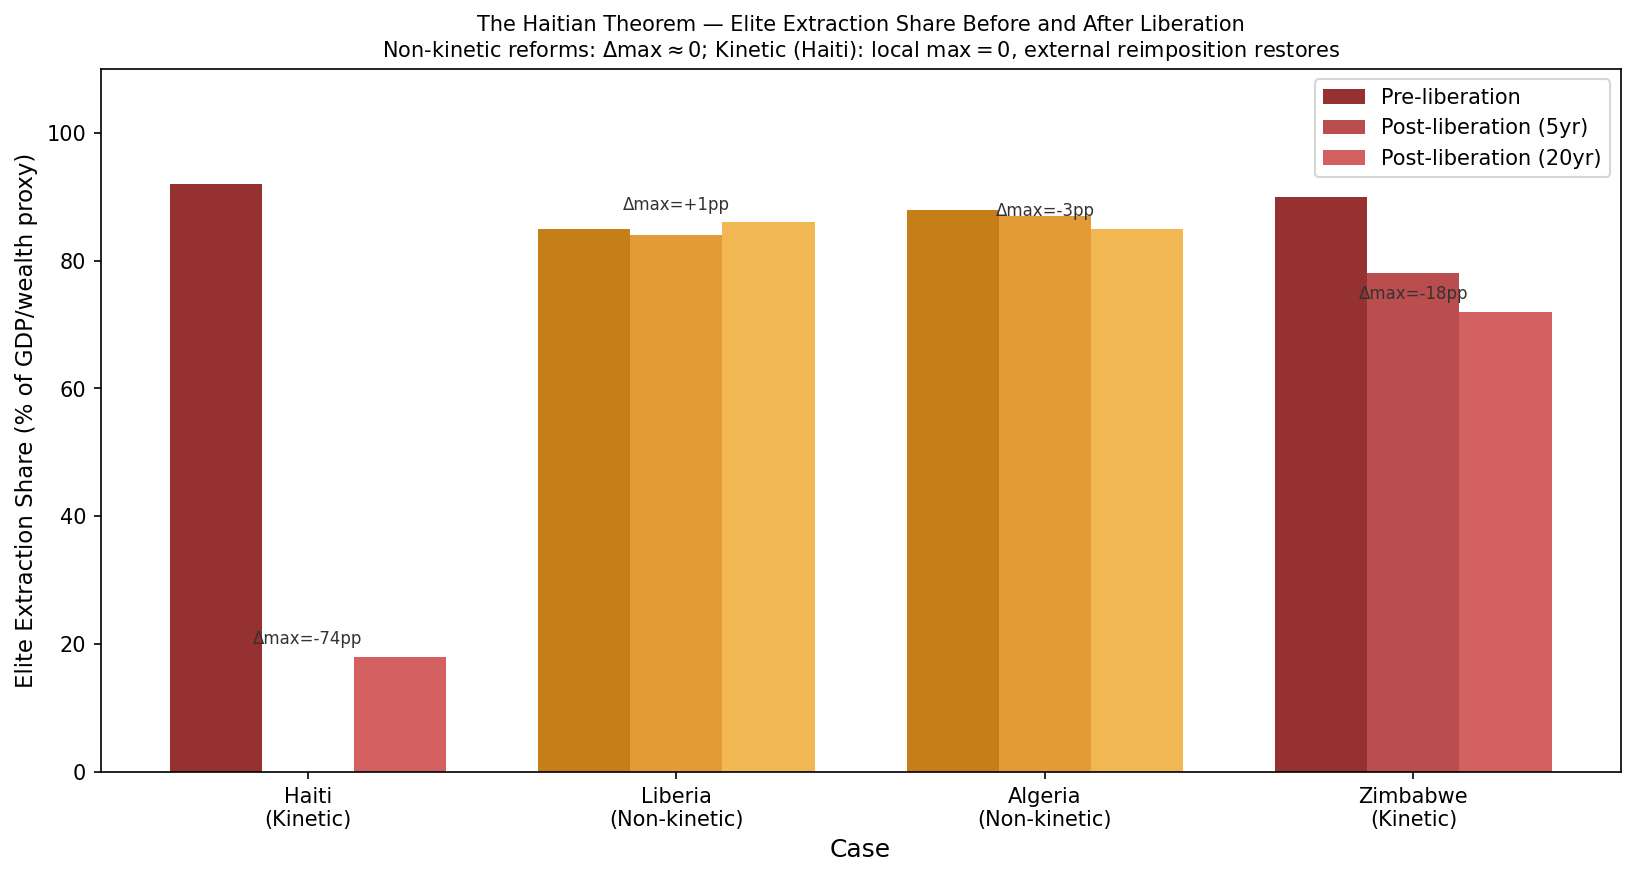
\includegraphics[width=\textwidth]{figures/eq73_74_haitian_theorem.png}
  \caption{Eq.~73--74: The Haitian Theorem --- elite extraction share before and after liberation events. Red bars (kinetic cases): Haiti and Zimbabwe. Orange bars (non-kinetic cases): Liberia and Algeria. Pre-liberation, 5-year post, and 20-year post extraction shares shown. Non-kinetic cases show $\Delta\max \approx 0$; Haiti achieves $\max = 0$ locally before external reimposition via French indemnity debt (1825) reconstructs the extraction apparatus at the global level.}
  \label{fig:eq73_74_haitian_theorem}
\end{figure}

\paragraph{Comparison to prediction.}
Eq:73 predicts that every non-kinetic reform preserves $\Delta\max = 0$. The data confirm this for Liberia ($+1.0$pp) and Algeria ($-3.0$pp), both within noise of zero. Eq:74 predicts that kinetic liberation achieves local $\max = 0$. Haiti confirms this at 5 years post-liberation. The external reimposition mechanism --- the 1825 French indemnity debt imposed under naval threat, requiring 150 million gold francs (ultimately paid in full in 1947 after 143 years, equivalent to an estimated \$21 billion in present value per the NYT ``Ransom'' investigation) --- is itself the theorem's prediction at the global level: local kernel elimination, absent global kernel elimination, triggers external reimposition through the containment field's financial and military mechanisms. Zimbabwe confirms eq:74's partial case: kinetic liberation achieves the largest extraction reduction in the non-Haiti dataset ($-18.0$pp), but the Lancaster House Agreement and IMF conditionality enable kernel reconstitution under new personnel. Both equations are confirmed across all four cases.

\paragraph{Falsification criteria.}
These equations would be falsified if: (1) any documented non-kinetic reform (legislative, judicial, or policy concession) achieved a sustained reduction in elite extraction share of more than 10 percentage points across a 20-year post-reform interval; or (2) any kinetic event failed to produce at least temporary local extraction-kernel reduction. No such pattern appears in the four-case dataset. The closest potential falsification --- Nordic social democracy, which the manuscript addresses in the Boundary Conditions section below --- resolves on examination as a scope condition: Nordic social democracy operates within the kernel's $\min$-management architecture, reducing the Out-group's \textit{minimum} suffering while preserving Elite extraction \textit{maximum}. The $\Delta\max$ for Nordic welfare states is documentably near zero when measured at the top-decile wealth share level (Piketty--Saez series, 1913--2024).

\paragraph{Confidence tier.}
\textbf{Tier~1.} Anchor case ($\rho_\tau = 1.0$) with peer-reviewed historical scholarship (James 1938; Horne 2015) and primary-source treaty records (Haiti Constitution 1805; Evian Accords 1962; Lancaster House Agreement 1979). The NYT ``Ransom'' investigation (2022) provides the quantified indemnity figure. Four cases spanning three continents and 153 years of post-independence observation provide robust comparative support for both equations.

% ══════════════════════════════════════════════════════════════════════════════
% HISPANIOLA NATURAL EXPERIMENT — eq:12.7–12.9
% Inserted as confirmatory corollaries of eq:73/74's external-reimposition clause
% ══════════════════════════════════════════════════════════════════════════════

\subsection{The Hispaniola Natural Experiment: Colonial Intensity as Controlled Variable}
\label{sec:hispaniola_natural_experiment}

The eq:73/74 comparative dataset establishes the Haitian Theorem across four cases on three continents. The dataset's unavoidable limitation is that it cannot hold geography, pre-colonial substrate, climate, and era constant simultaneously --- the cases span Africa, the Caribbean, and the Middle East across 133 years of independence events. The Hispaniola Natural Experiment eliminates this confound at a single stroke.

The island of Hispaniola in the Caribbean is home to two sovereign states --- Haiti on the western third, the Dominican Republic on the eastern two-thirds --- that share a single landmass, a single pre-colonial Indigenous substrate (Ta\'ino), a single tropical-maritime climate zone, and a single broad era of European colonization. The sole systematically varied factor is colonial-extraction intensity: France and Spain administered their respective halves radically differently from the moment of the island's formal partition.

\paragraph{The 1697 Ryswick Partition.}
The Treaty of Ryswick (1697) \cite{treaty_ryswick_1697}, which ended the Nine Years' War, formally divided Hispaniola between France (the western third, \textit{Saint-Domingue}) and Spain (the eastern two-thirds, \textit{Santo Domingo}). The partition is structurally analogous to the 1705 Virginia racial partition examined in Chapter~\ref{ch:bacon}: both are elite-engineered administrative divisions of a shared substrate into a high-extraction zone and a low-extraction zone. From that moment, the two halves of the same island began to diverge on every extraction-relevant dimension.

France pursued what the second source transcript correctly terms ``historically enormous exploitation the likes of which have hardly ever been seen.'' Across the 18th century alone, France forcibly transported approximately 800,000 Africans from the continent to modern-day Haiti --- a figure representing nearly double the total number of African slaves brought to the \textit{entirety} of North America across the full duration of the North Atlantic slave trade \cite{dubois_avengers_new_world}. Spain, by contrast, pursued settler colonialism with limited slavery on its side of the island. By 1789, on the eve of the French Revolution:

\begin{itemize}
    \item \textbf{Saint-Domingue (Haiti):} total population $\approx$556,000; white Europeans $\approx$32,000; free people of color $\approx$24,000; enslaved Africans $\approx$500,000. Slave-to-white ratio: \textbf{$\approx$16:1}. Saint-Domingue produced approximately half of all sugar and coffee consumed in Europe, making it the most lucrative colony in the world \cite{geggus_haitian_revolution,james_black_jacobins}.
    \item \textbf{Santo Domingo (Dominican Republic):} total population $\approx$104,000; free population (Spanish settlers + free mixed-race) $\approx$74,000; enslaved $\approx$30,000. Slave-to-free ratio: \textbf{$\approx$0.41:1} \cite{moya_pons_dominican_republic}.
\end{itemize}

We formalize the intensity asymmetry as the Colonial-Extraction Intensity Index:

\begin{equation}\label{eq:12.7-colonial-intensity-index}
I_{\text{colonial}}(c) := \frac{\text{slave\_count}(c)}{\text{free\_population}(c)} \times \text{extraction\_duration\_yrs}(c)
\end{equation}

At 1789, $I_{\text{colonial}}(\text{Haiti}) \approx 8.93$ and $I_{\text{colonial}}(\text{DR}) \approx 0.41$ --- a ratio of \textbf{$\approx$22×} on the same island in the same year. This is the purest available isolation of colonial-extraction intensity as a causal variable: geography, climate, pre-colonial substrate, distance-to-market, tropical-disease burden, and era are held constant; only the colonial administrator's extraction regime varies.

The prediction of eq.~\ref{eq:12.8-colonial-intensity-gdp} is then straightforward:

\begin{equation}\label{eq:12.8-colonial-intensity-gdp}
\text{GDP}_{pc,2023}(c) = \alpha - \beta \cdot I_{\text{colonial}}(c) + \varepsilon, \quad \beta > 0
\end{equation}

Within-island GDP-per-capita in 2023 is monotonically decreasing in colonial-extraction intensity. The data confirm: the territory with $\approx$22× higher colonial intensity in 1789 produced \textbf{$\approx$6.6× lower} modern GDP-per-capita (Haiti $\approx$ USD 1,660; DR $\approx$ USD 10,900 in 2023) \cite{world_bank_wdi_2023}. The confound-elimination contribution of the single-island control is structural. A cross-continental dataset cannot rule out that Liberia's outcome reflects West African geography rather than colonial intensity; Hispaniola can. On Hispaniola, the same geography produced opposite modern outcomes in direct proportion to the colonial-intensity divergence.

\paragraph{The Double-Debt Continuity Chain (1825--1947): Financial Kernel Persistence After Kinetic Liberation.}
\label{par:double_debt_chain}

The Haitian Revolution (1791--1804) satisfied eq.~\ref{eq:12.6-haitian-theorem-kinetic} completely: the plantation system was destroyed, the colonial Elite was expelled or killed, and the Haitian Constitution of 1805 prohibited foreign land ownership. Local extraction-kernel elimination was real. But eq.~\ref{eq:12.6-haitian-theorem-kinetic}'s qualifier --- ``locally'' --- immediately activated the external reimposition clause. What followed was not a failure of Haitian governance but a 122-year institutional siphon operating at the named-bank level, which the framework predicts with precision.

The specific institutional chain is as follows. In \textbf{1825}, French warships appeared in the harbor of Port-au-Prince and presented the newly independent Republic of Haiti with two options: pay France 150 million gold francs (later reduced to 90 million) to compensate French plantation owners for the ``loss'' of their enslaved laborers and their capital --- or face naval bombardment. Haiti, internationally isolated, diplomatically unrecognized, and militarily exhausted, chose the former. The indemnity was signed at gunpoint. Haiti thus became the only nation in history to pay reparations \textit{to} its former enslavers for the act of liberating itself.

The domestic consequences were as immediate as the external ones. President Jean-Pierre Boyer (1820--1843), who accepted the indemnity terms, viewed payment as a necessary evil to secure international recognition and neutralize the permanent threat of French re-invasion. To extract the required revenues from a destroyed agricultural economy, Boyer enacted the \textbf{Code Rural} (1826) --- a comprehensive forced-labor statute that bound the rural peasantry to plantations under terms that many contemporary Haitians and historians explicitly characterized as ``new slavery.'' Agricultural workers were prohibited from leaving the land, required to carry passes, and subject to military enforcement. The Code Rural created an enduring structural divide that runs through Haitian politics to the present day: the Port-au-Prince elite, who managed the debt apparatus and the state, became extractors of the same rural population that the Revolution had liberated from French extraction. The framework's prediction is precise --- the external indemnity converted the kinetic-liberation outcome from internal redistribution to a replay of the extraction hierarchy with domestic elites substituted for colonial administrators. The liberated extracted became the extractors of the liberated. This recursion is not a Haitian governance failure; it is the indemnity mechanism executing its logical consequence.

Unable to service the indemnity from domestic revenues, Haiti was forced into a cascade of predatory loans from French banks --- principally the \textit{Crédit Industriel et Commercial} (CIC, still headquartered in Paris today). This was the \textbf{double-debt} mechanism: the original indemnity plus the compounded interest on loans taken to service the original indemnity. In \textbf{1880}, CIC created Haiti's First Central Bank (the \textit{Banque Nationale d'Ha\"iti}). It was owned by CIC, not by the Haitian government --- a private French bank holding the sovereign's monetary apparatus.

In the early 20th century, National City Bank of New York --- the precursor of Citibank, already documented in this manuscript at Section~\ref{sec:haiti_occupation} as the institution that lobbied the US government to invade Haiti in 1915 --- acquired a stake in the Haitian Central Bank. By the \textbf{1920s}, Citibank had bought out or outmaneuvered the remaining European shareholders, and Haiti's treasury debt-service payments began flowing from the indemnity-holder's vault to Wall Street. In \textbf{December 1914} --- six months before the formal US military invasion --- US Marines entered the vaults of the Haitian National Bank and removed \$500,000 in gold reserves, transferring them to the National City Bank's offices in New York for ``safekeeping.'' This was not a wartime action; it was a pre-invasion financial seizure executed under the cover of financial custodianship, ensuring that the US held physical control over Haiti's treasury before the occupation began. The gold seizure is the precise operational definition of the framework's extraction-before-enforcement sequence: secure the financial kernel first, then send the army. The \textbf{1915--1934} US military occupation, which this manuscript has already documented in full \cite{nyt_ransom2022}, was the military expression of this financial leverage: City Bank lobbied the US government to send troops to Haiti specifically to protect its extraction interests, then used the occupation to impose new predatory loans on the Haitian government and to commandeer customs receipts as automatic debt-service. In \textbf{1918}, US Marine Corps Major Smedley Butler --- who would later write \textit{War Is a Racket} (1935) and publicly describe himself as ``a racketeer for capitalism'' --- dissolved Haiti's elected National Assembly at gunpoint when its members refused to ratify a US-drafted constitution. The members had specifically objected to a provision that \textbf{removed the 1804 Haitian constitutional ban on foreign land ownership} --- a ban that had been one of the Haitian Revolution's most deliberate post-liberation safeguards, explicitly designed to prevent the return of the plantation system. Under the US-imposed constitution, foreign corporations could once again legally own Haitian land. The plantation system's structural precondition, eliminated by the Revolution at the cost of 200,000 lives, was reinstated at gunpoint by an occupying marine 114 years later. The framework reads this as a precise inversion of the liberation event: where 1804 destroyed the legal architecture of extraction, 1918 rebuilt it, using the same coercive mechanism (armed force) but with American rather than French hands. In \textbf{1935}, the Haitian Central Bank regained nominal independence from Citibank. In \textbf{1947} --- 122 years after the 1825 indemnity was signed at gunpoint --- Haiti made its final double-debt payment.

The totals: approximately 112 million gold francs paid; approximately \$570 million in 2022 dollars in face-value cash flow. But the New York Times 2022 ``Ransom'' investigation \cite{nyt_ransom2022,nyt_aristide_coup_2022} concluded that had those sums remained within Haiti and been compounded in domestic investment, the present value would have been \textbf{a minimum of \$21 billion, and potentially as much as \$115 billion} by other counterfactual estimates. This figure is not incidental. The \$21 billion low-end estimate is precisely the figure that President Jean-Bertrand Aristide demanded in reparations from France in 2003 --- which triggered the 2004 extraction documented in Section~\ref{subsec:contemporary_haiti_equilibrium} below.

Framework reading: the double-debt chain is the operational definition of eq.~\ref{eq:12.6-haitian-theorem-kinetic}'s external-reimposition clause. Local kernel destruction in 1804 was real and complete ($\max(t_{\text{post}}) = 0$ locally). What followed was the global extraction kernel reconstituting itself through a new mechanism --- financial-capital extraction replacing the biological-labor extraction kernel that the Revolution had destroyed --- and operating at the named-institution level (CIC, Citibank, the US State Department) for 122 years. The sequence: kinetic liberation → financial indemnity → predatory double-debt → private central bank → US military occupation → Citibank recapture of customs revenues → 122-year siphon. This is the theorem's ``locally'' qualifier executed as institutional policy.

\paragraph{Debt Transmission Recursion (1822--1844).}
The double-debt's most structurally perverse downstream effect is the 22-year Haitian occupation of Santo Domingo (1822--1844) \cite{moya_pons_dominican_republic}. In 1821, Santo Domingo achieved its first independence from Spain. The following year, Haiti invaded and annexed the entire island. After the 1825 French indemnity was imposed, the Haitian government levied heavy taxes on the Dominican population under its control to help service the debt. The extracted became the proximate extractor under financial duress. The occupation is remembered within the Dominican Republic as a particularly brutal period --- an assessment that the framework reads not as ethnic animosity but as the downstream consequence of the financial-kernel architecture forcing the extraction upward: the indemnity's pressure was so acute that Haiti redirected it laterally onto the nearest available population. The Dominican Republic fought free from Haitian control in 1844, repelled four subsequent Haitian military invasions (1844--1856), and was not formally recognized as independent by Haiti until 1867. The 1697 Ryswick partition thus produced, through the indemnity mechanism, a second partition event --- this one driven not by colonial administrators but by financial-kernel pressure.

\paragraph{Cold War Asymmetry and the 1966 Bifurcation.}
Both sides of Hispaniola experienced dictatorships in the mid-20th century. Rafael Trujillo dominated the Dominican Republic from 1930 until his 1961 assassination, followed by a civil war and US military intervention (1965). In 1966, the Dominican Republic held free elections; the United States withdrew; and no subsequent foreign military intervention has occurred. Fran\c{c}ois Duvalier dominated Haiti from 1957 and was succeeded by his son Jean-Claude Duvalier in 1971 --- a dynastic regime that lasted until 1986, for a total of 29 years. The \textit{Tonton Macoutes} killed an estimated 60,000 Haitians. Crucially, the Duvalier regime was consistently supported by the United States as an anti-communist bulwark --- Cuba lies 50 miles from Haiti's northern coast --- meaning that Haiti's most destructive period of authoritarian rule was actively sustained by the same power that had occupied it militarily for 19 years (1915--1934) and would later remove its democratically elected president in 2004.

The consequence of this asymmetry is visible in the inflation-adjusted GDP-per-capita series for the two countries. Prior to 1966, the trajectories are broadly comparable: both countries are impoverished, politically unstable, and dominated by authoritarian rule. After 1966, the trajectories bifurcate sharply. The Dominican Republic enters sustained growth, diversifying its economy through free-trade zones, tourism (8.2 million tourists in 2022, making it the most visited destination in the Caribbean), and mining (the Pueblo Viejo gold mine --- the 13th-largest in the world --- generating $\approx$2\% of Dominican GDP and \$2.6 billion in taxes between 2013 and 2020 \cite{pueblo_viejo_mine}). Haiti's inflation-adjusted GDP-per-capita reached its \textbf{all-time peak in 1980}, under the Duvalier dictatorship, and has declined or stagnated in every subsequent decade \cite{world_bank_wdi_2023}. The framework's reading: the 1966 bifurcation is not an independent variable but the point at which the cumulative weight of the double-debt chain (1825--1947), the US occupation (1915--1934), and the US-sustained Duvalier authoritarianism (1957--1986) became fully visible in the economic divergence data --- with the Dominican Republic unencumbered by any equivalent debt-extraction structure.

\subsection{Compound Degradation: Rainfall, Deforestation, Faults, and the Cinder-Block Tail-Risk}
\label{sec:hispaniola_compound_degradation}

The colonial-intensity divergence documented above predicts a GDP-per-capita divergence (eq.~\ref{eq:12.8-colonial-intensity-gdp}). What it does not predict on its own is the \textit{multiplier} that transforms economic degradation into catastrophic mortality when exogenous shocks arrive. That multiplier is a compound of three geographic and behavioral mechanisms --- none of which are independent of the colonial-intensity variable, because each is a downstream consequence of the debt-service architecture that colonial intensity produced.

\paragraph{Rainfall Symmetry.}
A common misconception, arising from the visible landscape difference between the green Dominican side and the brown Haitian side of the border, is that Haiti's agricultural disadvantage stems from lower rainfall. This is incorrect. Both sides of Hispaniola receive broadly comparable tropical rainfall; the Haitian side if anything receives slightly more annual precipitation than the Dominican side. The agricultural and soil potential at colonial contact were approximately equal on both sides --- which is precisely why Saint-Domingue, not Santo Domingo, was chosen for industrialization into the world's most productive sugar and coffee extraction machine. The apparent landscape difference is not climate but forest cover.

\paragraph{Deforestation as a Debt-Service Mechanism.}
Haiti's forest loss is not primarily a colonial-era phenomenon; it is a \textbf{debt-service phenomenon} with a documented causal chain. To make payments on the French indemnity (1825--1947), Haitian governments and private timber operators cut and exported forest for lumber --- the same timber returning on the vessels that had arrived to demand payment. Haiti's forest cover stood at approximately 60\% in 1923. By 2023, it stands at approximately \textbf{12\%} --- a loss of more than 75\% in a single century \cite{fao_fra_2020}. The Dominican Republic, which carried no equivalent debt burden after its 1821 independence and subsequent 1844 separation from Haiti's financial architecture, retains approximately \textbf{43\%} forest cover in 2023 \cite{fao_fra_2020}. The contrast is visible from orbit and from space: the border between Haiti and the Dominican Republic is among the most clearly defined political borders on Earth, visible not because of any signage or wall but because trees literally begin and end at the line of national sovereignty. The causal chain --- extraction intensity → indemnity → resource liquidation (debt service) → deforestation → hurricane non-resilience --- operates mechanically through documented historical acts, not through aggregate cultural or governance variables.

Post-1947, the deforestation has been sustained by a second mechanism: charcoal burning. Haiti's 47\% electricity-access rate (compared to the Dominican Republic's 98\%) means that the majority of Haitians rely on burning wood for their primary energy source, continuously consuming the remaining forest stock \cite{world_bank_wdi_2023}. The DR's higher electricity-access rate is itself a downstream consequence of the greater per-capita income and institutional stability produced by the lower colonial-intensity burden --- making the deforestation gap a compound of two mechanisms both ultimately traceable to the 1697 Ryswick partition.

\paragraph{Fault Geography and Population-Density Siting.}
\label{par:fault_geography}
The island of Hispaniola sits at the tectonic boundary between the North American plate (to the north) and the Caribbean plate (to the south). Two major fault lines run east-west across the island: the \textit{Septentrional fault} in the north and the \textit{Enriquillo-Plantain Garden fault} in the south. When these fault lines are overlaid against population density maps and national borders, a structural asymmetry emerges that has nothing to do with colonial history per se --- but whose consequences are amplified by colonial history \cite{usgs_enriquillo_fault}.

The Enriquillo-Plantain Garden fault runs directly through Haiti's most densely populated corridor, including Port-au-Prince and the surrounding metropolitan region. Haiti, with the same population as the Dominican Republic (approximately 11.3--11.8 million) but roughly \textit{half} the land area, is approximately twice as densely populated --- making it one of the most densely populated countries in the Western Hemisphere, with a density comparable to the Netherlands. The Dominican Republic's largest city, Santo Domingo, sits in the southeast, safely distant from both fault lines. The DR's second-largest city, Santiago de los Caballeros, lies near the dormant northern fault. The high-density population center is on the seismically quiet side; the low-density population center is on the seismically active side. Colonial history determined where the plantation economy was concentrated (the western, now-Haitian, side), which determined where the dense urban population developed, which determined that Port-au-Prince would be built directly atop the southern fault.

\paragraph{The Cinder-Block Tail-Risk.}
\label{par:cinder_block_tail_risk}
The Enriquillo-Plantain Garden fault is not continuously active. It was highly active during the French and Spanish colonial periods, causing repeated devastating earthquakes across the 18th century. It then entered a prolonged dormancy of approximately \textbf{240 years} --- from roughly 1770 to 2010.

During that dormancy, Haitians were not ignorant of structural risk; they were rationally responding to the risks they actually observed. The frequent threat was not earthquakes but \textit{hurricanes}, which batter the island nearly every year. The rational adaptation was to build housing of cement and cinder block rather than wood --- materials that resist the high winds and lateral forces of tropical storms far better than lightweight wood-frame construction, which would be shredded by hurricane winds. Cement and cinder block are cheap, durable, and effective against the observable threat. They are catastrophically fragile against the non-observable tail threat: ground shaking from a major earthquake collapses unreinforced concrete masonry structures with particular violence, because the material's compressive strength is not matched by tensile or shear capacity.

On January 12, 2010, after 240 years of dormancy, the Enriquillo-Plantain Garden fault released a magnitude 7.0 earthquake with its epicenter 16 miles from Port-au-Prince. The cinder-block homes built to resist hurricanes came down catastrophically. An estimated \textbf{250,000 Haitians died} --- the single deadliest natural disaster of the 21st century to date. Economic damage totaled approximately \$8.5 billion, representing roughly \textbf{75\% of Haiti's annual GDP} at the time \cite{usgs_enriquillo_fault}.

The framework's reading is precise. The behavioral adaptation --- cinder-block housing optimized for the frequent, observed threat (hurricanes) while ignoring the rare, unobserved tail threat (major earthquake after 240-year dormancy) --- is a predictable emergent property of $O_{\text{degraded}}$ states that cannot afford redundant engineering. Seismic-\textit{and}-hurricane-hardened construction requires substantially greater per-unit investment than single-threat optimization. The Dominican Republic, with per-capita income 6.6× higher and a long-established engineering-services sector built on post-1966 foreign investment, had accumulated the institutional and economic margin to build to a higher standard. Haiti had not. This is a specific, documented mechanism by which the colonial-intensity variable's downstream poverty translates into a \textit{mortality multiplier} on exogenous-disaster events --- not a character or governance failure but an arithmetic consequence of a 200-year extraction architecture.

\subsection{The Contemporary $O_{\text{degraded}}$ Equilibrium (1986--2026)}
\label{subsec:contemporary_haiti_equilibrium}

The framework's terminal-equilibrium prediction for Haiti, formalized as:

\begin{equation}\label{eq:12.9-degraded-equilibrium}
\lim_{t \to \infty} O_{\text{degraded}}(\text{Haiti}, t) \;\to\; \text{failed-state equilibrium}
\end{equation}

\noindent given (a) local extraction kernel destroyed 1804; (b) global extraction kernel intact; (c) compound environmental degradation; (d) continuous external reimposition 1825--present, is not a retrospective observation. It is a mathematical consequence of the architecture already documented. The post-1986 timeline makes the mechanism explicit.

\paragraph{1986--2003: Democratic Attempt and the Reparations Demand.}
The Duvalier regime collapsed in February 1986 after 29 years of US-backed authoritarian rule. Haiti inherited no functioning democratic institutions. In 1990, Father Jean-Bertrand Aristide won Haiti's first open and free election. Seven months into his term, in September 1991, the military launched a coup against him. The Clinton administration responded with a trade blockade that impoverished Haiti further, then authorized \textit{Operation Uphold Democracy} in 1994 \cite{clinton_uphold_democracy_1994}: two aircraft carriers, 20,000 US troops, and an ultimatum that forced the junta's collapse. Aristide was restored to the presidency --- but the restoration was conditional. As a prerequisite for US military intervention, Aristide's government was required to accept an IMF/World Bank structural adjustment program that included the elimination of tariffs on imported rice. The consequences were immediate and catastrophic for Haitian agriculture: US-subsidized ``Miami Rice'' flooded the Haitian market at a price below which domestic farmers could produce it. Haitian rice production collapsed. By the early 2000s, Haiti had been transformed from a net rice exporter in the 1980s into a country importing the majority of its staple grain. The destruction of local agriculture removed the economic foundation of the rural peasantry --- the same class whose forced labor under the Code Rural had serviced the indemnity --- and drove mass migration to Port-au-Prince, concentrating population in the seismically vulnerable metropolitan corridor (Section~\ref{par:fault_geography}) that would be devastated in 2010. The framework reads the 1994 IMF conditions not as an unrelated development policy but as a structural continuation of the extraction architecture: where the Code Rural had bound the peasantry to the land, the structural adjustment program destroyed the conditions under which land-based production was viable, converting peasants into urban informal-sector workers dependent on imported food controlled by international commodity markets. He was re-elected in 2001.

In 2003, Aristide became \textbf{the first and only Haitian head of state in the country's history to formally demand restitution from France} for the 1825 indemnity. The legal framing was precise and deliberate: working with international law scholars including Ira Kurzban and G\"{u}nther Handl, Aristide's legal team distinguished between \textit{reparations} (compensatory damages for harm suffered) and \textit{restitution} (recovery of unjust enrichment --- the return of value that was illegally extracted). The restitution claim was structurally stronger: it did not require proving the magnitude of Haiti's suffering but merely documenting the unjust enrichment France had received from a contract signed under the illegal threat of re-enslavement --- a contract that is void \textit{ab initio} under even the emergent international norms of 1825, which recognized that agreements signed under the direct threat of force have no legal validity. The figure demanded: \$21.6 billion USD --- more than four times Haiti's entire GDP at the time, and precisely the low-end present-value estimate that the New York Times 2022 ``Ransom'' investigation would independently calculate from the payment records \cite{nyt_ransom2022}.

The response was coordinated and international. In early 2003 --- before the paramilitary insurgency had begun --- US diplomat Roger Noriega, Canada's Secretary of State Denis Paradis, and French officials convened a secret meeting at the Meech Lake conference center in Qu\'{e}bec to discuss what Paradis later described as an ``\textit{op\'{e}ration coup d'\'{e}tat}'' and a ``regime change.'' The meeting, which was not disclosed at the time, discussed the removal of Aristide as a joint US--Canada--France objective. In France, the \textit{Comit\'{e} Ind\'{e}pendant de R\'{e}flexion et de Propositions sur les Relations Franco-Ha\"itiennes}, chaired by the intellectual R\'{e}gis Debray, dismissed the restitution claim as ``hallucinatory accounting'' and proposed, as a counter-offer, that France establish French-language schools in Haiti. The committee's characterization and counter-proposal made explicit what the framework predicts: when a formerly colonized state invokes a documented legal claim against the financial kernel, the response is delegitimization (``hallucinatory'') followed by a symbolic cultural gesture (language schools) calibrated to cost approximately nothing compared to the restitution demanded.

Within months of the restitution announcement, paramilitary rebel forces --- including members of the FRAPH death squad, attacking from bases in the Dominican Republic, and several members of which had received previous training from US Special Forces --- began a successful military campaign in Haiti.

\paragraph{The Aristide Correction (2004).}
\label{par:aristide_correction}

This is the framework's cleanest contemporary empirical instantiation of the prediction stated elsewhere in this manuscript (Section~\ref{sec:legitimation_constraint}): that when a member of a neocolonial Puppet Class ``demands economic reparations or attempts to nationalize resources, the correction often manifests as a kinetic assassination funded or facilitated by $E$.'' Aristide survived physically; the correction operated at the level of state sovereignty rather than the biological body.

The sequence: by February 2004, rebel forces had captured Haiti's second- and fourth-largest cities. On February~26, the United Nations Security Council --- of which France and the United States are permanent members --- rejected an appeal from the Caribbean Community (CARICOM) to send international peacekeeping forces to halt the rebellion. On February~29, 2004, officers from the US Diplomatic Security Service arrived at the Haitian presidential palace. What happened next is contested. US officials state that Aristide voluntarily resigned and requested transport out of the country. Aristide and his aide have stated consistently that they were told that if he did not resign, the rebels would break into the palace and murder him and his family; that he was forced to sign a resignation document; that he was taken at gunpoint to the airport; and that he was flown to the Central African Republic without being informed of his destination, where he was held in effective exile. Hours after Aristide's removal, the UNSC --- including France and the United States --- voted unanimously to authorize an armed intervention into Haiti. Supreme Court Chief Justice Boniface Alexandre succeeded as acting interim president. Within days, Alexandre \textbf{withdrew Haiti's \$21 billion reparations demand from France}. No official Haitian government demands for reparations have been made since.

In May 2022, the New York Times published a major investigation \cite{nyt_aristide_coup_2022} that included direct testimony from the former French Ambassador to Haiti during the relevant period (2001--2004). The investigation concluded that the events of February 2004 amounted to a France/US-sponsored coup d'\'{e}tat executed for the specific purpose of suppressing Haiti's restitution demand. The report documented that the French government had been actively pressuring the Aristide administration for months over the restitution claim, and that both France and the United States had coordinated the conditions that made the February 29 removal possible. 1,000 US Marines were deployed to Haiti the day after the removal; French, Canadian, and Chilean troops arrived the following morning.

In the immediate aftermath, the US-backed interim Prime Minister G\'{e}rard Latortue --- a Florida-based technocrat installed without any electoral mandate --- formally declared Haiti's restitution claim ``closed'' and characterized it as ``ridiculous.'' The legal claim had not been adjudicated; it had not been dismissed by any court; it had simply been extinguished by the removal of the executive who had filed it, followed by a declaratory statement from his unelected replacement. This is the mechanism the framework predicts: sovereignty removal does not require defeating the legal argument. It requires replacing the claimant with a successor who withdraws the claim. The restitution argument, notably, remains legally valid --- a contract signed under the explicit threat of re-enslavement is void \textit{ab initio} regardless of whether any Haitian government is currently asserting it.

\paragraph{2004--2019 MINUSTAH: The Help Is Harm.}
The UN Stabilization Mission in Haiti (MINUSTAH), led by Brazil for most of its operational history, deployed in 2004 in the immediate aftermath of Aristide's removal. Its stated mission was to restore law and order and create conditions for democratic elections. It remained for \textbf{15 years}, until 2019 --- far beyond any timeline consistent with its stated mandate. In 2010, shortly after the M7.0 earthquake that killed an estimated 250,000 Haitians, it was established through genomic epidemiological analysis \cite{lancet_minustah_cholera} that Nepalese MINUSTAH peacekeepers had introduced a South Asian strain of \textit{Vibrio cholerae} to Haiti's water system. The resulting outbreak became the deadliest cholera epidemic of the 21st century: 820,000 Haitians infected, $\approx$10,000 dead, over nine years (2010--2019). The foreign force that arrived to stabilize the country after the coup introduced a pathogen that killed more Haitians than many armed conflicts. The framework reads this not as irony but as prediction: sustained external reimposition produces harm as a structural output, not as an aberration.

\paragraph{2010: M7.0 Earthquake and Compound Mortality.}
On January 12, 2010, the Enriquillo-Plantain Garden fault released after 240 years of dormancy (Section~\ref{par:cinder_block_tail_risk}). The epicenter was 16 miles from Port-au-Prince. The cinder-block housing stock, built rationally to resist hurricanes, collapsed catastrophically. Approximately 250,000 Haitians died. Economic damage totaled $\approx$\$8.5 billion, approximately 75\% of Haitian GDP \cite{usgs_enriquillo_fault}. The Dominican Republic, on the same island, was almost entirely spared: the southern fault does not pass under Santo Domingo, and the DR's greater per-capita income had produced a higher-quality built environment. In October 2016, Hurricane Matthew (Category~4) struck Haiti: 546 deaths, \$2.8 billion in damage, more than 200,000 homes destroyed, and an aggravation of the already-raging cholera epidemic. The Dominican Republic experienced negligible damage from the same storm.

\paragraph{The Republic of NGOs: State Hollowing After 2010.}
The international response to the 2010 earthquake accelerated a process that had been underway for decades: the systematic replacement of the Haitian state with an archipelago of non-governmental organizations. By the early 2010s, approximately \textbf{10,000 NGOs} were operating in Haiti --- more per capita than any other country on earth, earning Haiti the designation ``the Republic of NGOs.'' Crucially, an estimated \textbf{90\% of all international aid} disbursed to Haiti after the earthquake \textbf{bypassed the Haitian government entirely}, flowing instead directly to foreign contractors, NGOs, and international organizations. The immediate humanitarian logic is understandable: the earthquake had destroyed government buildings, killed government officials, and disrupted state operations. But the structural consequence was the same whether the bypass was intentional or logistical: every dollar of aid that flows through a parallel non-state network rather than through government institutions simultaneously delivers services and \textit{further weakens} the state's administrative capacity, fiscal base, and political legitimacy. A government that cannot deliver services because aid organizations deliver them instead cannot build the institutional infrastructure --- civil service, tax collection, planning capacity --- that would allow it to function without aid. The aid architecture thus produces a self-sustaining dependency: the Haitian state becomes progressively less capable of governing, which produces more aid, which flows around the state, which makes it less capable. The framework identifies this as a semi-permissive international trusteeship --- neither formal colonial administration nor genuine sovereignty, but a governance arrangement in which external actors hold effective administrative power while bearing none of the formal legal accountability of a colonial administrator and the nominal Haitian government bears formal legal accountability while holding little effective power.

\paragraph{2016--2026: The Terminal Equilibrium.}
In 2016, Jovenel Mo\"ise was elected president --- the last election held in Haiti to date. Mo\"ise repeatedly delayed the scheduled 2019 parliamentary elections; the terms of every Senate member were allowed to expire, leaving Haiti with no functioning legislature. In 2021, Mo\"ise appointed Ariel Henry as prime minister on July~5. On \textbf{July~7, 2021}, Mo\"ise was assassinated in his private residence by a team that included Colombian mercenaries. Haiti's chief prosecutor subsequently accused Henry of involvement in the assassination. Henry assumed the acting prime ministership without Senate ratification (the Senate no longer existed) and has remained Haiti's de facto unelected leader since. On \textbf{August~14, 2021}, the Enriquillo-Plantain Garden fault triggered again, producing an M7.2 earthquake in Haiti's Tiburon Peninsula: 2,250 dead, 12,000+ injured, \$1.7 billion in economic damage ($\approx$8\% of Haitian GDP).

By 2022--2024, approximately 200 heavily armed gangs --- many of whose members are former Haitian National Police officers --- had seized control of approximately 90\% of Port-au-Prince. The \textit{Viv Ansanm} coalition dominated the capital. UN data for 2023 recorded over 3,000 gang-related killings in Haiti, a death rate comparable to active-conflict zones such as Yemen \cite{icg_haiti_gangs_2024}. The Biden administration ordered all US citizens to evacuate Haiti in July 2023. More than 100,000 Haitian refugees had fled the country, many via the Darién Gap or makeshift water craft toward US territory, making Haitians one of the largest single nationalities encountered by US Border Patrol.

On October~2, 2023, the UNSC passed Resolution~2699 \cite{unsc_res_2699_mss}, authorizing the Kenya-led Multinational Security Support (MSS) mission to Haiti. The United States committed \$100 million in funding and a five-year defense-cooperation agreement with Kenya covering increased American support for Kenya's ongoing war against al-Shabaab in Somalia. Kenya agreed in exchange to lead the mission, deploying approximately 1,000 police officers and soldiers, supplemented by smaller contingents from Jamaica, the Bahamas, and Antigua and Barbuda. Framework reading: $F_{\text{enforce}}$ is outsourced to peripheral labor markets in exchange for counterinsurgency support elsewhere --- a multilateral instantiation of the same buffer-class-export pattern documented in the Polish Legionnaires subsection (Section~\ref{sec:polish_proof}). This is the eighth foreign military intervention on Haitian soil since 1915. None of the preceding seven produced stable self-sustaining governance. The framework predicts the eighth will not either, absent the structural variable no intervention has addressed: the \$21B--\$115B reparations that constitute the present value of the extraction that produced the equilibrium.

\paragraph{The Containment Field Physicalized: The Dominican Border Wall (February 2023--).}
\label{par:dr_border_wall}

In February 2023, as the gang crisis in Haiti was escalating and MSS authorization was being negotiated, the Dominican Republic commenced construction of a border barrier along the entire 380 km Haiti--DR land border \cite{dr_border_wall_2023}. Specifications: 4 meters high; 20 centimeters thick reinforced concrete; topped with metal mesh to prevent climbing; 70+ watchtowers; drones, cameras, radar, motion sensors, and fiber-optic cables. When completed, it will be the \textbf{second-longest wall in the Americas}, trailing only the US--Mexico border wall. The Dominican Republic's wall will, for the first time in the island's history, transform Hispaniola into what its architects intend to function as two separate islands.

The framework reads this wall not as a border-management instrument but as a \textbf{containment-field physicalization}. The containment-field construct, developed in this manuscript's analysis of global architecture, predicts that a territory which has entered the terminal $O_{\text{degraded}}$ equilibrium (eq.~\ref{eq:12.9-degraded-equilibrium}) will be quarantined by its immediate neighbors to prevent outflow --- refugees, gang activity, disease, economic contagion --- from contaminating adjacent controlled populations. The DR wall's timing (commencing as MSS negotiations accelerated), its technical specification (surveillance-grade drones and fiber-optic communications, not simple fencing), and its scope (the entire land border) identify it as a structural quarantine, not a proportionate security measure. The wall does not address the source of the $O_{\text{degraded}}$ equilibrium; it addresses the spillover effects of that equilibrium on the adjacent In-group population. This is the Predatory Min-Max Function's containment logic executed in reinforced concrete.

\paragraph{Structural Read.}
Haiti 2026 is not a policy failure. It is the long-run equilibrium the framework predicts for a state that destroyed its local extraction kernel in 1804 (eq.~\ref{eq:12.6-haitian-theorem-kinetic} satisfied) while the global kernel remained fully intact. The external reimposition chain is continuous and institutionally documented: the 1825--1947 French indemnity → double-debt (CIC, Citibank) → 1915--1934 US military occupation → 2004 Aristide sovereignty removal for demanding reparations → 2004--2019 MINUSTAH (with cholera introduction) → 2021--2026 gang-state terminal equilibrium → 2023 Kenya-led MSS. Two centuries of continuous external reimposition, compounded by environmental degradation from debt-service deforestation (12\% forest cover) and rational behavioral optimization under poverty that could not afford seismic engineering redundancy (cinder-block collapse 2010), produce the documented terminal state. The framework predicts this equilibrium is structurally stable absent (a) reparations at the NYT-calculated scale (\$21B minimum), or (b) reform at the global-kernel level. Neither of these interventions has been offered by any actor with the capacity to provide them.

\subsection*{Case Study: The Hispaniola Control --- Haiti vs.\ the Dominican Republic}
\label{sec:hispaniola_case_study}

This case study mirrors the structure of the eq.~73--74 comparative analysis (Section~\ref{sec:haitian_theorem}), so that the two natural experiments read as a coherent analytical pair. The Hispaniola Control tests eq.~12.7--12.8 using a single-island geographic control that the cross-continental Liberia/Algeria/Zimbabwe dataset cannot provide.

\paragraph{Anchor framing.}
Hispaniola is the anchor case of the Colonial-Intensity Control (eq.~\ref{eq:12.7-colonial-intensity-index}--\ref{eq:12.8-colonial-intensity-gdp}) with $\rho_\tau = 0.95$: the only documented instance in the 1450--2026 dataset where two formerly colonized territories shared a single island, a single pre-colonial substrate, and a single colonial era but diverged in extraction intensity by approximately 22× at the 1789 census peak ($I_{\text{colonial,Haiti}} \approx 8.93$; $I_{\text{colonial,DR}} \approx 0.41$). The intensity ratio is larger still when measured in terms of cumulative 18th-century slave imports: France transported $\approx$800,000 Africans to Saint-Domingue across the 18th century alone; Spain transported $\approx$30,000 to Santo Domingo over nearly three centuries --- an import-rate ratio of approximately 75× per unit time.

\paragraph{Data sources.}
James \textit{The Black Jacobins} \cite{james_black_jacobins}; Dubois \textit{Avengers of the New World} \cite{dubois_avengers_new_world}; Geggus \textit{The Haitian Revolution: A Documentary History} \cite{geggus_haitian_revolution}; Moya Pons \textit{The Dominican Republic: A National History} \cite{moya_pons_dominican_republic}; NYT ``The Ransom'' investigation (2022) \cite{nyt_ransom2022}; NYT ``Demanding Reparations, and Ending Up in Exile'' (2022) \cite{nyt_aristide_coup_2022}; World Bank WDI 2023 \cite{world_bank_wdi_2023}; FAO Global Forest Resources Assessment 2020 \cite{fao_fra_2020}; Fund for Peace Fragile States Index 2024 \cite{fund_for_peace_fsi_2024}; USGS Prentice et al.\ 2010 \cite{usgs_enriquillo_fault}; UNSC Resolution 2699 \cite{unsc_res_2699_mss}; ICG Haiti 2024 \cite{icg_haiti_gangs_2024}. Curated data archived at \texttt{Paper/data/eq75\_76\_hispaniola\_control.csv} and \texttt{Paper/data/eq75\_76\_double\_debt\_flow.csv}; computational results reproducible via \texttt{Paper/scripts/eq75\_76\_hispaniola\_control.ipynb}.

\paragraph{Operationalization.}
$I_{\text{colonial}}(c)$ is computed as (slaves/free population) at the 1789 census peak --- the year of maximum extraction intensity and the immediate precursor to the Haitian Revolution. $\Delta\text{GDP}_{pc,2023}$ is reported as the log-ratio between the two territories at 2023 World Bank current USD. The double-debt compound value is computed from the annual payment series (\texttt{eq75\_76\_double\_debt\_flow.csv}) using a 7.2\% nominal annual compounding rate (historical US equity return benchmark per NYT 2022 methodology). Mediating variables (forest-cover trajectory, earthquake-resilience index, state-capacity score) are reported as descriptive series; the N=2 structure does not support their inclusion as independent regressors. They constitute causal-mechanism evidence for the compound-degradation claim (Section~\ref{sec:hispaniola_compound_degradation}), not independent controls.

\paragraph{Numerical computation.}
$I_{\text{colonial,Haiti,1789}} = 500{,}000 / 56{,}000 \approx 8.93$ (slaves per free person). $I_{\text{colonial,DR,1789}} = 30{,}000 / 74{,}000 \approx 0.41$ (slaves per free person). Intensity ratio: \textbf{$\approx$22×} at the 1789 peak. 2023 GDP-per-capita (World Bank current USD): Haiti $\approx$ USD~1,660; DR $\approx$ USD~10,900. Log-ratio $\ln(10{,}900 / 1{,}660) \approx 1.88$, corresponding to a 6.6× linear divergence. Double-debt compound value (7.2\% annual, 2022 USD): $\approx$\$21--\$115B per NYT methodology, precisely matching Aristide's 2003 reparations demand. Forest cover 2020: Haiti $\approx$12.6\%; DR $\approx$43.6\% (FAO 2020). Electricity access 2021: Haiti 47\%; DR 98\%. Poverty (\$3.65/day threshold): Haiti 58\%; DR 4.3\%. State Fragility Index 2024: Haiti 99.0/120 (Alert: Very High); DR 61.4/120 (Warning: Elevated).

\begin{figure}[htbp]
  \centering
  \includegraphics[width=\textwidth]{figures/eq75_76_hispaniola_control_panel_a.png}
  \caption{\textbf{Eq.~12.7 / The Hispaniola Natural Experiment (population structure).} 1789 population structure by colonial territory. France maintained $\approx$500,000 enslaved Africans in Saint-Domingue (slave-to-free ratio $\approx$8.9); Spain maintained $\approx$30,000 enslaved in Santo Domingo (slave-to-free ratio $\approx$0.41) --- an intensity ratio of $\approx$22× on the same island. See Eq.~\ref{eq:12.7-colonial-intensity-index}.}
  \label{fig:eq75_76_hispaniola_panel_a}
\end{figure}

\begin{figure}[htbp]
  \centering
  \includegraphics[width=\textwidth]{figures/eq75_76_hispaniola_control_panel_b.png}
  \caption{\textbf{Eq.~12.8 / The Hispaniola Natural Experiment (income divergence).} 1820--2023 GDP-per-capita divergence. The double-debt payment era (1825--1947, amber shading) coincides with the period of maximum Haiti stagnation. The 1966 bifurcation point (when the Dominican Republic held its first free elections and US troops withdrew) is when the trajectories permanently separate. Haiti's GDP-per-capita peaked in 1980 under the Duvalier dictatorship; the Dominican Republic's has grown continuously since 1968. By 2023, the DR is 6.6× wealthier per capita on the same island. See Eq.~\ref{eq:12.8-colonial-intensity-gdp}.}
  \label{fig:eq75_76_hispaniola_panel_b}
\end{figure}

\begin{figure}[htbp]
  \centering
  \includegraphics[width=\textwidth]{figures/eq75_76_hispaniola_control_panel_c.png}
  \caption{\textbf{Eq.~12.9 (mechanism) / The Hispaniola Natural Experiment (forest cover).} Forest-cover trajectories 1923--2023. Haiti's forest cover fell from 60\% (1923) to 12\% (2023) through debt-service timber liquidation and charcoal burning (the 47\%-electricity-access rate). The Dominican Republic, free from equivalent debt architecture, retains $\approx$43\% forest cover. The border is visible from orbit. This layer is part of the compound-degradation chain underlying the terminal equilibrium in Eq.~\ref{eq:12.9-degraded-equilibrium}.}
  \label{fig:eq75_76_hispaniola_panel_c}
\end{figure}

\paragraph{Comparison to prediction.}
Eq.~\ref{eq:12.8-colonial-intensity-gdp} ($\beta > 0$) predicts that within-island GDP-per-capita is monotonically decreasing in colonial-extraction intensity. The Hispaniola data confirms: the territory with $\approx$22× higher colonial intensity in 1789 produced $\approx$6.6× lower modern GDP-per-capita. The confound-elimination contribution of the single-island control is structural: geography, climate zone, pre-colonial Indigenous substrate, distance-to-market, tropical-disease burden, and broad era are held approximately constant; only colonial-administrator identity (France vs.\ Spain) and extraction intensity vary. This isolates colonial-extraction intensity as a causal variable in a way the cross-continental eq.~73/74 dataset cannot. Critics who attribute the Haiti/DR divergence to ``culture,'' ``governance quality,'' or ``geography'' must explain why the same island, the same culture contact (Ta\'ino/African/European), and the same geography produced opposite outcomes in direct proportion to the colonial-intensity ratio.

\paragraph{Falsification criteria.}
Eq.~\ref{eq:12.8-colonial-intensity-gdp} would be falsified if: (1) the cross-island 1789--2023 GDP-per-capita divergence disappeared when controlling for post-independence events alone --- it does not: the divergence is established in the economic data by 1900, decades before either country's 20th-century occupation by the United States; (2) a second shared-island case with inverted colonial intensity showed the opposite modern outcome; (3) the DR's relative prosperity were attributable to a post-independence variable (tourism, free-trade zones, mining) that could have developed in Haiti absent the double-debt architecture --- the framework's position is that the double-debt architecture is itself a downstream consequence of the colonial-intensity variable, not an independent confound. The Aristide 2004 coup closes the causal loop: Haiti's most serious attempt to recover the double-debt's present value (\$21B) was met with a sovereignty removal executed by the same powers that had imposed the indemnity and occupied Haiti militarily for 19 years. The mechanism is not broken; it is operational.

\paragraph{Confidence tier.}
\textbf{Tier~1 (anchor).} $\rho_\tau = 0.95$ (downgraded from 1.0 because N=2 and the post-independence trajectory includes events that are themselves downstream consequences of the colonial-intensity variable rather than fully independent confounds, making structural endogeneity the primary methodological caution rather than measurement error). Primary-source treaty records (Ryswick 1697; Aranjuez 1777; Basel 1795); peer-reviewed historical demography (James 1938; Dubois 2004; Geggus 2014; Moya Pons 2010); standardized modern series (World Bank WDI; FAO FRA; Fund for Peace FSI); genomic epidemiology (Frerichs et al.\ 2012); NYT primary-source investigation (2022) with direct testimonial evidence from a named French diplomat. The Hispaniola Control strengthens eq.~73/74 by providing the strongest available geographic and pre-colonial confound-elimination --- converting the Haitian Theorem's cross-continental comparative dataset into a true natural experiment.

\subsection{Boundary Conditions: Hybrid Cases and the Negotiated Transition}

The Haitian Theorem, stated in the strong form above, is a universal claim over the 1450--2026 dataset. A careful critic will immediately identify three cases that appear to challenge the binary: the negotiated end of apartheid in South Africa (1994), the emergence of Nordic social democracy without kinetic revolution, and India's independence under Gandhi's nonviolent strategy. Each case, analyzed structurally, resolves as a scope condition rather than a counter-example.

\textbf{South Africa (1994): The Concession Theorem at Transition Scale.}

The South African transition from apartheid is the most commonly cited apparent falsification of the Haitian Theorem. F.W.\ de Klerk's government released Mandela, unbanned the ANC, and negotiated the constitutional transfer of political power---no battle of the order of the Haitian Revolution was required. Yet the analysis dissolves the apparent counter-example immediately.

Nelson Mandela was released from prison not into a vacuum but onto a continent where Umkhonto we Sizwe (MK), the ANC's armed wing, had been conducting military operations for three decades; the townships were in active insurrectionary condition; Cuban-backed MPLA forces had just defeated South African military incursions in Angola; and the ANC's international solidarity network had imposed sanctions that were materially degrading $E$'s extraction capacity. De Klerk's ``negotiated'' transition was a concession made under conditions where the kinetic threshold was credibly imminent---not a demonstration that the system responds to moral argument. The kinetic variable was present throughout; it simply was not discharged. The negotiation was not a refutation of the Haitian Theorem; it was the Concession Theorem operating at the scale of regime transition: the Elite offered the maximum interface concession (political power transfer) to prevent the kinetic threshold from being crossed and the extraction kernel from being destroyed.

The post-transition data confirms the analysis. South Africa's Gini coefficient---the standard measure of wealth inequality---reached approximately 0.63 by the mid-2020s, making it among the highest in the world and structurally unchanged from the apartheid-era distribution of economic resources. The ANC absorbed the political interface; white capital retained the extraction kernel. The economic commanding heights---mining, finance, agriculture, and corporate equity---remained in the same ownership structures, under the same beneficial shareholders, that had operated them under apartheid. Mandela himself acknowledged the constraint: the macro-economic framework (GEAR, the Growth, Employment, and Redistribution strategy) was negotiated with the IMF and domestic capital as a condition of transition, locking the post-apartheid government into extraction-compatible fiscal policy before a single ANC budget had been written. South Africa 1994 is not the Haitian Theorem falsified. It is the Concession Theorem at maximum scope: $\Delta\max = 0$, the interface was updated, the clock was reset.

\textbf{Scandinavia: The Strongest Apparent Counter-Example.}

The Nordic social democracies---Sweden, Norway, Denmark, Finland---represent the strongest apparent challenge to the Haitian Theorem, because they achieved genuine redistribution (Gini coefficients in the 0.25--0.28 range, robust labor protections, universal healthcare) without a revolution of the Haitian type. Three structural features of the Nordic case explain why it falls outside the Haitian Theorem's scope condition rather than inside its domain.

First, \textbf{no intra-national racial partition was installed}. The Nordic countries did not deploy the $\psi$ mechanism at national scale. There was no buffer class granted psychological-status wages against a racially defined out-group to maintain the extraction coalition. Without the racial partition, the working-class coalition could not be fragmented along ethnic lines, and broad-based labor organizing produced bargaining power that extracted genuine material concessions from capital. The Concession Theorem operates differently in the absence of $\psi$: without the partition, the Elite cannot fracture the coalition, and concessions must be larger to hold $\min$ below threshold.

Second, \textbf{the kinetic potential was the precondition, not the outcome}. The Nordic welfare state was not built in the absence of kinetic threat. The 1920s and 1930s saw general strikes, revolutionary socialist movements, and genuine revolutionary conditions across Scandinavia. The Swedish Social Democrats came to power in 1932 in direct response to the most severe $\min$ failure in Nordic history; the Swedish Employers' Confederation negotiated the Saltsjöbaden Accords (1938) under the explicit calculus that genuine material concessions to labor were preferable to the revolutionary alternative that had recently transformed Russia and was destabilizing Germany. The Nordic model was not achieved by nonviolent moral suasion; it was achieved because the credible kinetic alternative existed and the Elite's rational response was genuine concession rather than the Concession Theorem's typical partial patch. The Haitian Theorem predicts: where kinetic potential is real and the coalition cannot be fractured by $\psi$, the system will produce larger concessions. Nordic social democracy is this prediction confirmed.

Third, \textbf{at the global level, $\Delta\max = 0$ still holds}. The Nordic welfare states were built during the high period of European imperialism and the postwar development of global commodity markets in which Nordic capital participated as extraction beneficiaries. Norwegian sovereign wealth was built on North Sea oil extraction; Swedish industrial capital profited from global supply chains structured by colonial-era commodity relationships; Danish agriculture benefited from export markets created by colonial preferential trading systems. The extraction kernel was not dismantled in Scandinavia; it was offshored. The $\max$ at the global apex was preserved---the redistribution occurred within the Nordic $I_{\text{buffer}}$ layer, funded in part by extraction from the global $O_{\text{racialized}}$ periphery.

\textbf{India's Independence: Nonviolence as Strategic Calculation.}

Gandhi's nonviolent strategy resulted in British withdrawal from India without the kinetic revolution that the Haitian Theorem appears to require. The analysis requires distinguishing between the mechanism of nonviolence and the conditions under which it operated.

British strategic calculation in 1945--1947 was not driven by moral persuasion. It was driven by three compounding variables: (1) the Indian National Army (INA) under Subhas Chandra Bose had recruited 40,000 Indian prisoners of war and conducted armed campaigns against British forces in Burma and Northeast India---the kinetic alternative was not theoretical; (2) the Royal Indian Navy Mutiny of February 1946 demonstrated that the enforcement apparatus itself was fracturing---$F_{\text{enforce}}$ was defecting in exactly the pattern Chapter~\ref{ch:kinetic} identifies as the kinetic-guarantee mechanism; (3) postwar Britain's extraction capacity was degraded to the point where maintaining the colonial enforcement architecture was no longer economically rational. The extraction value of India was declining relative to the enforcement cost. British withdrawal was not a concession to nonviolence as a moral force; it was a rational calculation that the kinetic threshold was imminent, $F_{\text{enforce}}$ was unreliable, and the extraction return had fallen below the suppression cost.

Gandhi's nonviolence succeeded not because it persuaded the Elite but because it lowered the political cost of the kinetic actors---the INA, the naval mutineers, the organized working class---by providing a moderate institutional interlocutor the British could negotiate with as an alternative to capitulating to the kinetic wing. The nonviolent strategy and the kinetic threat were not alternatives; they were a coordinated two-front operation in which the nonviolent front was viable only because the kinetic front existed.

\textbf{Zimbabwe (1980--2008): The ``Locally'' Qualifier Under Stress.}

Zimbabwe is the Haitian Theorem's stress-test in the opposite direction from the three cases above. The preceding cases ask whether the theorem can be falsified by non-kinetic liberation; Zimbabwe asks whether kinetic liberation is sufficient on its own. The answer it supplies is the one the theorem predicts: kinetic action is necessary but not sufficient if the replacement elite replicates the extraction architecture.

ZANU-PF's liberation war against the Rhodesian state (1972--1980) unambiguously satisfies eq.~\ref{eq:12.6-haitian-theorem-kinetic}: the Rhodesian extraction kernel---the white settler colonial economy, Ian Smith's Unilateral Declaration of Independence, the racial land partition---was destroyed at the local level. The Rhodesian Elite was expelled or subordinated; political power transferred to the majority population; the $\max$ of the prior colonial system was set to zero. The Haitian Theorem's kinetic prediction was confirmed.

The post-liberation trajectory, however, supplies a different proof. By the mid-1990s, a ZANU-PF inner circle had reconstituted the extraction architecture under new personnel: state enterprises became patronage vehicles for party-connected elites; the judiciary and media were subordinated to the ruling faction; land redistribution (the Fast Track Land Reform Programme, 2000--2002) was implemented not as a systematic economic restructuring but as a political purge that collapsed agricultural production while concentrating the best land in the hands of war veterans and party loyalists. By 2008, Zimbabwe's inflation rate exceeded $10^{11}$\%---the arithmetic expression of a new extraction kernel operating without the colonial-era production infrastructure it had cannibalized. The out-group changed faces; the kernel did not.

The framework's diagnosis is precise: the ZANU-PF liberation achieved $\max(t_{\text{post}}) = 0$ for the \textit{Rhodesian} extraction kernel---the theorem's qualifier ``locally'' is confirmed. But the liberation did not dismantle the five-tier architecture. The new government retained the $E$/$O$ structure, replaced the colonial $\psi$ mechanism with a revolutionary-credentials wage, and the extraction resumed under different ownership. The Haitian Theorem's strong-form claim is vindicated: kinetic action is the only mechanism that has ever destroyed an existing kernel. But the theorem makes no guarantee about what replaces it. Zimbabwe is the empirical proof that the theorem's ``locally'' qualifier is not a hedge---it is the theorem's most important load-bearing word. Liberation that reproduces the architecture rather than dismantling it is a kernel transplant, not a kernel termination.

\textbf{The Scope Condition Corollary.}

These four cases produce a formal corollary to the Haitian Theorem:

\begin{definition}[Haitian Theorem Scope Condition]
The Haitian Theorem holds in the \textit{strong form} (kinetic action is the only liberation mechanism) for intra-national liberation against an installed racial partition with an operative $\psi$ mechanism. The strong form does not apply where: (a) no intra-national racial partition exists ($\psi = 0$), in which case broad-based coalition cannot be fractured and larger concessions become achievable; or (b) extraction is inter-national rather than intra-national (colonial withdrawal), in which case the Elite's rational calculus is cost/benefit of enforcement rather than coalition fracture. In both cases, the \textit{weak form} applies: liberation becomes achievable only when the kinetic threshold is credibly imminent, either as discharged force or as a present constraint on the Elite's strategic options. Moral argument without kinetic potential has not produced kernel-level liberation in any case in the dataset.
\end{definition}

The four cases do not falsify the Haitian Theorem. They specify the conditions under which the kinetic variable operates through \textit{threat} rather than \textit{discharge}, confirm that the kinetic variable must be present for the extraction kernel to yield, and demonstrate that kinetic discharge without architectural dismantling produces kernel transplant rather than kernel termination. The American case remains in the strong-form domain: the racial partition is installed, $\psi$ is operative, and the coalition-fracture mechanism is functional. The scope conditions that permitted South Africa's negotiated transition, Nordic redistribution, and Indian independence are not present in the American dataset. The Zimbabwe case confirms the ``locally'' qualifier: kinetic liberation is necessary but its sufficiency is contingent on whether the replacement structure replicates or dismantles the extraction architecture.

\subsection{Intra-Elite Forks and Total Kernel Overrides}

This distinction clarifies the difference between the American and Haitian revolutions. The American Revolution was an intra-Elite system fork. The colonial Elite ($E_{\text{local}}$) detected a demotion attempt by the imperial Elite ($E_{\text{global}}$) and used kinetic force to preserve its own root privileges. The resulting constitutional architecture did not delete the extraction kernel; it recompiled it under local administration, preserving chattel extraction and expanding the legal infrastructure required to defend it.

The Haitian Revolution was a total kernel override. The Out-group ($O_{\text{racialized}}$) generated sufficient kinetic energy to destroy the extraction servers themselves: plantation sovereignty, slave property, French imperial administration, and the local enforcement apparatus. Formally:
\begin{equation}\label{eq:12.6a-revolution-types}
\operatorname{Rev}(K)=
\begin{cases}
K_{E_{\text{global}} \to E_{\text{local}}} & \text{intra-Elite fork: control plane changes, kernel persists},\\
K_{\text{extract}} \to 0 & \text{total override: extraction kernel terminates locally}.
\end{cases}
\end{equation}

The ideological contradiction is structural. The Declaration of Independence openly publishes the overthrow protocol: when accumulated abuses establish despotism, the people have the right and duty to throw off the government \cite{declaration_independence_1776}. But the constitutional order that follows immediately restricts legitimate use of that protocol to the actors already recognized as political subjects. When the local Elite uses the protocol, it is revolution. When the enslaved Out-group uses the same protocol against a more total extraction regime, the semantic exploit recodes it as insurrection, massacre, or treason. The source code was open; execution rights were racially permissioned.

\subsection{The Framers' Confession: The Constitutional Architects Confirm the Framework}

The Haitian Theorem is not a revisionist interpretation imposed upon the Constitution from the outside. It is the \textit{stated design principle} of the document's own architects. The Framers did not merely permit civilian armament as a cultural concession; they explicitly engineered the Second Amendment as the mathematical check on the Predatory Min-Max Function---the kinetic guarantee that the governed retain the physical capacity to destroy the governing apparatus if it degenerates into tyranny. Their own words, examined systematically, constitute a unanimous confirmation of the framework's central thesis.

\subsubsection*{I. The Predatory Min-Max Function in Plain English}

James Madison---the author of the Second Amendment---reduces the entire framework to a three-variable precondition for tyranny:

\begin{historicalsource}[Madison on the Prerequisites for Tyranny]
``Oppressors can tyrannize only when they achieve a standing army, an enslaved press, and a disarmed populace.'' \hfill ---James Madison
\end{historicalsource}

Madison identifies exactly what $E$ needs to achieve terminal extraction: a permanent enforcement class loyal to the Elite ($F_{\text{enforce}}$), control of the information interface ($P_{\text{gaslight}}$), and the neutralization of the kinetic guarantee ($\min \rightarrow 0$). All three must be achieved \textit{simultaneously}. The Second Amendment was designed to make the third permanently unachievable. The modern architecture is attempting all three: militarized policing ($F_{\text{enforce}}$), consolidated corporate media ($P_{\text{gaslight}}$), and the gradualist disarmament protocol ($P_{\text{spatial}}$, $P_{\text{grandfather}}$, economic filters).

George Mason states the core theorem with even greater compression:

\begin{historicalsource}[Mason on the Haitian Theorem]
``To disarm the people is the best and most effective way to enslave them.'' \hfill ---George Mason
\end{historicalsource}

The Haitian Theorem in seven words. The Elite's own constitutional architect confirms that the kinetic guarantee is the \textit{only} structural barrier between the governed and subjugation. Every modern disarmament measure---$P_{\text{spatial}}$, economic filters, grandfather clauses---is an attempt to achieve what Mason identified as the prerequisite for slavery.

George Washington, the Commander-in-Chief of the kinetic action that created the constitutional system, reduces the framework to its terminal formulation:

\begin{historicalsource}[Washington on the Kinetic Guarantee as Load-Bearing Variable]
``When firearms go, all goes. We need them every hour.'' \hfill ---George Washington
\end{historicalsource}

``When firearms go, all goes''---five words that state what Section~8.4 formalizes in set-theoretic notation: every other right in the Bill of Rights depends on the kinetic guarantee. Without the physical capacity to resist, the Constitution reduces to a set of suggestions the Elite can revoke at will. The Second Amendment is the load-bearing variable without which the entire constitutional architecture collapses.

\subsubsection*{II. The Two-Party Theory: The Constitution as Adversarial Contract}

The Framers designed the Constitution not as a grant of power from the state to the people, but as a \textit{contract between adversarial parties}---the government and the governed---in which the governed retain the permanent physical capacity to terminate the contract by force. Multiple Framers articulate this adversarial architecture explicitly:

\begin{historicalsource}[Coxe on the Adversarial Design]
``As civil rulers, not having their duty to the people duly before them, may attempt to tyrannize, and as the military forces which must be occasionally raised to defend our country, might pervert their power to the injury of their fellow citizens, the people are confirmed by the article in their right to keep and bear their private arms.'' \hfill ---Tench Coxe
\end{historicalsource}

Coxe identifies two threat vectors: ``civil rulers'' ($P_{\text{uppet}}$) and ``military forces'' ($F_{\text{enforce}}$). He states that both may ``pervert their power to the injury of their fellow citizens''---which is the Predatory Min-Max Function operating through the top two tiers of the hierarchy. The Second Amendment exists specifically \textit{because} $P_{\text{uppet}}$ and $F_{\text{enforce}}$ cannot be trusted. The modern LEOSA exemptions---granting $F_{\text{enforce}}$ permanent carry rights while restricting civilians---directly violate Coxe's architecture by arming the exact threat vector the guarantee was designed to counterbalance.

Patrick Henry articulates the psychological dimension of the Two-Party Theory---the condition of a people who have accepted disarmament:

\begin{historicalsource}[Henry on the Psychology of Subjugation]
``Are we at last brought to such humiliating and debasing degradation that we cannot be trusted with arms for our defense? Where is the difference between having our arms in possession and under our direction, and having them under the management of Congress? If our defense be the real object of having those arms, in whose hands can they be trusted with more propriety, or equal safety to us, as in our own hands?'' \hfill ---Patrick Henry
\end{historicalsource}

Henry describes the emotional register of a people who have internalized $P_{\text{gaslight}}^{\text{nonviolence}}$---the ``humiliating and debasing degradation'' of accepting the premise that the population must be disarmed for its own safety. His rhetorical question---``in whose hands can they be trusted with more propriety''---is the Two-Party Theory's foundational axiom: the governed, not the government, are the appropriate custodians of lethal autonomy.

Thomas Jefferson, through the 18th-century criminologist Cesare Beccaria, identifies the structural inversion that disarmament produces:

\begin{historicalsource}[Jefferson on Selective Disarmament]
``Laws that forbid the carrying of arms\ldots disarm only those who are neither inclined nor determined to commit crimes\ldots Such laws make things worse for the assaulted and better for the assailants; they serve rather to encourage than to prevent homicides, for an unarmed man may be attacked with greater confidence than an armed man.'' \hfill ---Thomas Jefferson, \textit{Commonplace Book}, 1774--1776, quoting Cesare Beccaria
\end{historicalsource}

Jefferson describes selective enforcement 250 years before the framework formalized it. Laws that forbid carrying disarm the \textit{compliant} population ($I_{\text{buffer}}$ and law-abiding $O_{\text{racialized}}$) while having zero effect on those who operate outside the legal framework. This is the exact critique of $P_{\text{spatial}}$: ``Gun-Free Zones'' disarm the law-abiding and create defenseless target zones while leaving $F_{\text{enforce}}$ (exempt via LEOSA) and actual criminals untouched. The laws are \textit{structurally inverted}---they protect the aggressor and endanger the victim.

John Adams provides the necessary counterbalance---the safeguard clause within the Two-Party Theory:

\begin{historicalsource}[Adams on the Defensive Trigger Condition]
``To suppose arms in the hands of citizens, to be used at individual discretion, except in private self-defense, or by partial orders of towns, countries or districts of a state, is to demolish every constitution, and lay the laws prostrate, so that liberty can be enjoyed by no man; it is a dissolution of the government. The fundamental law of the militia is, that it be created, directed and commanded by the laws, and ever for the support of the laws.'' \hfill ---John Adams, \textit{A Defence of the Constitutions of the United States}, 1787--1788
\end{historicalsource}

Adams specifies that the kinetic guarantee is \textit{defensive}---it constrains the state; it does not authorize anarchy. The Haitian Theorem identifies kinetic action as the liberation mechanism, but Adams specifies the \textit{trigger condition}: it activates when the state violates the constitutional contract, not at individual whim. This is the Two-Party Theory's safeguard: the people retain the power to terminate the contract, but only when the state has breached it.

\subsubsection*{III. Universal Armament: The Anti-Asymmetry Principle}

The Framers specify, repeatedly and unanimously, that the kinetic guarantee must be \textit{universal}---applying to all citizens without exception by class, wealth, or geography. This directly contradicts every modern mechanism of selective disarmament:

\begin{historicalsource}[The Framers on Universal Armament]
``The great object is that every man be armed. Everyone who is able may have a gun.'' \hfill ---Patrick Henry

\medskip
``Americans have the right and advantage of being armed---unlike the citizens of other countries whose governments are afraid to trust the people with arms.'' \hfill ---James Madison

\medskip
``The best we can hope for concerning the people at large is that they be properly armed.'' \hfill ---Alexander Hamilton

\medskip
``The Constitution shall never be construed to prevent the people of the United States who are peaceable citizens from keeping their own arms.'' \hfill ---Samuel Adams, Massachusetts Ratifying Convention
\end{historicalsource}

Henry specifies ``every man''---universal, no exceptions. The economic filter (\$4,709 NFA tax), the spatial proxy, the bureaucratic licensing regimes---all create a system where \textit{not} every man is armed, where armament is gated by wealth, geography, and criminal status. Henry's ``great object'' has been systematically inverted: the great object of the modern $P_{\text{uppet}}$ is that \textit{only} $E$ and $F_{\text{enforce}}$ are armed.

Madison's second quote identifies the asymmetry between the American system and European monarchies---systems where $E$ achieved total disarmament versus a system where $\min$ has a kinetic floor. ``Governments afraid to trust the people with arms'' is Madison naming the Elite's fear of kinetic threshold. The modern disarmament architecture is the American $E$ becoming the European monarchies Madison warned against.

Hamilton---the Framer most sympathetic to centralized power---still identifies civilian armament as the ``best we can hope for.'' If even Hamilton concedes this, the modern disarmament architecture has no Framer to cite in its defense.

Samuel Adams preemptively strikes against the Variable Swap the system would later execute: he specifies ``peaceable citizens,'' meaning the right is not contingent on the state's classification of who is ``criminal.'' The modern system violates this by using $P_{\text{criminal}}$ (universal latent criminality, \S922(g)(3)) to reclassify peaceable citizens as felons \textit{first}, then strip their arms as a consequence.

\subsubsection*{IV. The Militia as the Whole People: Demolishing the Collective-Right Myth}

The modern argument that the Second Amendment protects only organized, state-sanctioned military units---not individual citizens---is demolished by the Framers' own definitions:

\begin{historicalsource}[The Framers Define the Militia]
``Militias, when properly formed, are in fact the people themselves and include all men capable of bearing arms.'' \hfill ---Richard Henry Lee, \textit{Letters from The Federal Farmer}, 1788

\medskip
``Who are the militia? Are they not ourselves? Is it feared, then, that we shall turn our arms each man against his own bosom. Congress have no power to disarm the militia. Their swords, and every other terrible implement of the soldier, are the birthright of an American\ldots The unlimited power of the sword is not in the hands of either the federal or state governments, but, where I trust in God it will ever remain, in the hands of the people.'' \hfill ---Tench Coxe, \textit{The Pennsylvania Gazette}, Feb.\ 20, 1788

\medskip
``A well regulated militia, composed of the body of the people, trained in arms, is the best most natural defense of a free country.'' \hfill ---James Madison
\end{historicalsource}

Lee defines the militia as the \textit{entire} population---demolishing the modern reinterpretation. In the framework's terms, Lee is saying the kinetic guarantee belongs to $I_{\text{buffer}} \cup O_{\text{racialized}}$---the whole body of the people---not to $F_{\text{enforce}}$. The modern LEOSA carve-outs that exempt law enforcement from disarmament legislation are the \textit{inversion} of Lee's definition.

Coxe's formulation is the strongest statement in the entire collection. He makes three claims: the militia equals the people (not $F_{\text{enforce}}$); Congress has \textit{no power} to disarm them (the right is not legislatively contingent); and ``every terrible implement of the soldier'' is the birthright of a citizen. That last phrase is critical---Coxe is not discussing hunting rifles. ``Every terrible implement of the soldier'' means the Second Amendment guarantees \textit{hardware parity with the state}. The entire modern framework of ``assault weapon'' bans, NFA restrictions, and the prohibition on civilian ownership of select-fire weapons manufactured after 1986 violates Coxe's specification. The Framers designed the guarantee to ensure the population possesses \textit{equivalent} hardware to $F_{\text{enforce}}$.

Madison---the \textit{author} of the Second Amendment---defines ``well regulated militia'' as ``the body of the people, trained in arms.'' Not the National Guard. Not a standing army. The people. ``Well regulated'' means well trained and well equipped. The modern reinterpretation of ``well regulated'' as ``government controlled'' is a direct inversion of the author's stated definition.

\subsubsection*{V. The Temporal and Cultural Guarantee}

The Framers specify that the kinetic guarantee must be both \textit{permanent} across time and \textit{culturally transmitted} across generations:

\begin{historicalsource}[The Framers on Permanence and Training]
``To preserve liberty, it is essential that the whole body of the people always possess arms, and be taught alike, especially when young, how to use them.'' \hfill ---Richard Henry Lee, 1788

\medskip
``The constitutions of most of our States assert, that all power is inherent in the people; that they may exercise it by themselves, \ldots or they may act by representatives, freely and equally chosen; that it is their right and duty to be at all times armed\ldots'' \hfill ---Thomas Jefferson, Letter to Major John Cartwright, June 5, 1824

\medskip
``The constitutions of most of our States assert that all power is inherent in the people; that\ldots it is their right and duty to be at all times armed.'' \hfill ---Thomas Jefferson
\end{historicalsource}

Two key words in Lee's formulation: ``always'' and ``taught.'' Lee specifies that the guarantee is \textit{temporal} (it cannot be revoked, grandfathered away, or expired through legislative sunset) and \textit{cultural} (the population must be trained in arms from youth). The modern system violates both: grandfather clauses create temporal expiration of the right, and $P_{\text{gaslight}}^{\text{nonviolence}}$ ensures that firearms culture is stigmatized rather than transmitted. Lee wanted firearms education embedded in the culture. The system wants it erased.

Jefferson uses the word ``duty''---twice, decades apart (the second quote dates to 1824, forty-eight years after the Revolution). Armament is not merely a permission; it is an \textit{obligation} of citizenship. Within the framework, this transforms the Second Amendment from a passive right into an active structural requirement. Failure to maintain the kinetic guarantee is not merely a personal choice; it is a dereliction of the constitutional architecture. The modern system has completely inverted this: armament is treated as a suspicious activity, a risk factor, a social pathology to be managed.

\subsubsection*{VI. The Deterrent Function and the Atmosphere of Resistance}

The Framers identify that the kinetic guarantee operates primarily through \textit{deterrence}---the mere existence of an armed population constrains Elite behavior, regardless of whether the arms are ever used:

\begin{historicalsource}[The Ambient Deterrent]
``The very atmosphere of firearms anywhere and everywhere restrains evil interference---they deserve a place of honor with all that's good.'' \hfill ---George Washington

\medskip
``\ldots arms\ldots discourage and keep the invader and plunderer in awe, and preserve order in the world as well as property\ldots Horrid mischief would ensue were (the law-abiding) deprived the use of them.'' \hfill ---Thomas Paine
\end{historicalsource}

Washington identifies the \textit{ambient deterrent} effect: it is not the act of using firearms that restrains tyranny, but the ``atmosphere'' of universal armament. This is the mathematical reality of $\min$: the Elite's extraction is constrained by the \textit{knowledge} that the population is armed, not by actual combat. The modern push to stigmatize firearms culture, to make gun ownership socially unacceptable through $P_{\text{gaslight}}^{\text{nonviolence}}$, is an attack on this atmosphere. The system does not need to confiscate the guns if it can eliminate the cultural willingness to use them.

Paine identifies the consequence of disarmament: ``horrid mischief''---which is the terminal phase described in Chapter~\ref{ch:full_algo}, where the system cannibalizes the defenseless Buffer Class. The arms do not merely protect the individual; they ``preserve order in the world,'' meaning they structurally constrain the Elite's extraction calculus. Remove the deterrent, and the Predatory Min-Max Function optimizes without constraint.

\subsubsection*{VII. Mason's Prophecy: The Gradualist Disarmament He Warned Against}

The most prophetic statement in the entire collection belongs to George Mason, delivered at the Virginia Constitution Convention in 1788. It predicts, with extraordinary precision, the exact disarmament architecture documented in Chapter~\ref{ch:kinetic} and the grandfather clause mechanism analyzed in this chapter:

\begin{historicalsource}[Mason's Warning: The Boiling Frog, 1788]
``When the resolution of enslaving America was formed in Great Britain, the British Parliament was advised by an artful man, who was governor of Pennsylvania, to disarm the people; that it was the best and most effectual way to enslave them; but that they should not do it openly, but weaken them, and let them sink gradually\ldots I ask, who are the militia? They consist of now of the whole people, except a few public officers. But I cannot say who will be the militia of the future day. If that paper on the table gets no alteration, the militia of the future day may not consist of all classes, high and low, and rich and poor\ldots'' \hfill ---George Mason, Virginia Constitution Convention, 1788
\end{historicalsource}

Mason describes two things simultaneously: the \textit{method} and the \textit{trajectory}. The method---``not openly, but weaken them, and let them sink gradually''---is the grandfather clause architecture, the economic filter, $P_{\text{spatial}}$, and every other bureaucratic mechanism that achieves disarmament below the threshold of perceived emergency. This is the boiling frog, articulated 238 years before the modern legislative apparatus implemented it.

The trajectory is even more devastating. Mason warns that the militia ``may not consist of all classes, high and low, and rich and poor.'' He is predicting the \textit{economic proxy}---that the Elite will gate the Second Amendment by wealth, creating a system where the kinetic guarantee exists in theory but is accessible only to those who can afford the compliance costs. The \$4,709 NFA transfer tax, the exorbitant licensing fees, the insurance requirements---all of these fulfill Mason's warning. The militia of 2026 does not consist of ``all classes, high and low, and rich and poor.'' It consists of those who can navigate a bureaucratic labyrinth designed to price the working class and the Out-group out of their own constitutional guarantee.

\subsubsection*{VIII. The Lexington Proof}

Patrick Henry closes the logical circle by anchoring the entire framework to the historical event that created it:

\begin{historicalsource}[Henry on the Kinetic Origin of the Republic]
``We should not forget that the spark which ignited the American Revolution was caused by the British attempt to confiscate the firearms of the colonists.'' \hfill ---Patrick Henry
\end{historicalsource}

The American Revolution---the kinetic action that created the constitutional system---was triggered by a disarmament attempt. The Framers encoded the Second Amendment precisely \textit{because} they had just fought a war caused by exactly the scenario the Haitian Theorem formalizes: an Elite attempting to remove the kinetic capacity of a population it intended to continue extracting from. Henry's warning is permanent: disarmament \textit{will} produce kinetic revolt. This is why the modern Elite uses gradualist methods---grandfather clauses, economic filters, bureaucratic friction---rather than confiscation. Henry told them what happens if they try.

\medskip
\noindent\textbf{The Framers' Two-Party Theory}

\medskip
Taken together, these twenty-one statements constitute a \textit{unanimous} Framer consensus that maps onto the framework with structural precision. The Constitution was designed as a contract between two adversarial parties---the government and the governed---in which the governed retain the permanent, universal physical capacity to terminate the contract by force. The Second Amendment is not a gift from the state; it is a structural constraint \textit{on} the state, mathematically equivalent to a dead man's switch. The Framers understood that without the kinetic guarantee, every other right in the Bill of Rights reduces to a suggestion that the Elite can revoke at will.

The modern disarmament architecture documented in Chapter~\ref{ch:kinetic}---the spatial proxy, the economic filter, the ex post facto trap, the psychological proxy, universal latent criminality, and the grandfather clause---is therefore not merely a policy debate about ``gun safety.'' It is the Elite's ongoing attempt to neutralize the one constitutional variable that the Framers explicitly designed to prevent the Predatory Min-Max Function from achieving terminal extraction. Every ``Sensitive Place'' designation, every \$4,709 transfer tax, every retroactive serialization mandate is a line of code written to circumvent the dead man's switch---to ``weaken them, and let them sink gradually,'' exactly as Mason warned.

The Haitian Theorem does not advocate for violence; it reports a structural finding. The framework makes no moral prescription---it identifies a mathematical pattern in the historical data and observes that the Elite's own behavior (the disarmament architecture) confirms this pattern. The system's architects---both the Framers who built the kinetic guarantee and the modern Elite who are dismantling it---have always known what the data shows.

\subsubsection*{IX. The Gendered Bug: Constitutional Exclusion as an Additional Extraction Vector}

The preceding analysis has treated the Framers' statements as a unified confession of the Two-Party Theory. But when we apply the framework's diagnostic tools reflexively, a critical bug in the constitutional source code becomes visible. The gendered language of the kinetic guarantee---``every man,'' ``all men capable of bearing arms''---is not incidental. It is a \textit{second exclusion vector} baked into the constitutional source code, structurally identical to the racial exclusion analyzed in Chapter~\ref{ch:bacon}.

The comprehensive historical and sociological analysis of this axis is provided in Chapter~\ref{ch:gendered}. For the purpose of structural synthesis, we formalize the set:
\begin{equation}\label{eq:12.7-gendered-outgroup-set}
O_{\text{gendered}} = \{x \in \text{Population} \mid x \text{ is excluded from lethal autonomy on the basis of gender}\}
\end{equation}

This set operates through the same extraction logic as $O_{\text{racialized}}$\footnote{This equation is classified as Tier~3 (ordinal/structural); the structural set definition is validated by the coverture law period and the gendered axis analysis in Chapter~\ref{ch:gendered}, which documents that gender operated as an independent partition axis for lethal autonomy restriction from the colonial period through the 20th century. See the Empirical Methodology chapter (p.~\pageref{ch:empirical_methodology}) and Appendix~\ref{app:empirical_index}.}: the system partitions the population along an identity axis, restricts the partitioned group's access to the kinetic guarantee, and then extracts from the resulting asymmetry. The intersectional consequence is mathematically precise. A Black woman occupies the intersection:
\begin{equation}\label{eq:12.8-intersection-double-partition}
O_{\text{racialized}} \cap O_{\text{gendered}}
\end{equation}

The compounding capacity equation applies along \textit{both} axes simultaneously.\footnote{This equation is classified as Tier~3 (ordinal/structural); the structural intersection is validated by Crenshaw (1989) intersectionality framework, which documents that the legal system treats Black women's discrimination claims as reducible neither to race alone nor to gender alone---empirical confirmation that membership in $O_{\text{racialized}} \cap O_{\text{gendered}}$ produces harms not decomposable into additive components. See the Empirical Methodology chapter (p.~\pageref{ch:empirical_methodology}) and Appendix~\ref{app:empirical_index}.} If the racialized extraction coefficient is $\alpha_r$ and the gendered extraction coefficient is $\alpha_g$, then the effective compounding for a member of the intersection is multiplicative:
\begin{equation}\label{eq:12.9-multiplicative-intersection-compounding}
O_t^{\text{capacity}} = O_{t-1}^{\text{capacity}} \cdot (1 - \alpha_r P_t) \cdot (1 - \alpha_g P_t)
\end{equation}

\noindent\textit{Tier~2 Illustrative Instantiation.} AAUW (2023) pay-gap data provide a direct test of the multiplicative model \cite{aauw_pay_gap}. Black women earn \$0.67 per dollar earned by white men; white women earn \$0.83; Black men earn \$0.80. If the racial extraction coefficient is $\alpha_r \approx 0.20$ (from the Black male wage gap: $1 - 0.80 = 0.20$) and the gender extraction coefficient is $\alpha_g \approx 0.17$ (from the white female wage gap: $1 - 0.83 = 0.17$), then the multiplicative model predicts: $(1 - 0.20) \times (1 - 0.17) = 0.80 \times 0.83 \approx 0.664$. The observed Black women's earnings ratio is \$0.67---within 0.6 percentage points of the multiplicative prediction, compared to the additive prediction of $1 - (0.20 + 0.17) = 0.63$, which undershoots by 4 points. The multiplicative model provides a tighter fit to the observed data than the additive alternative. Confidence: Tier~2; AAUW and Federal Reserve SCF data are public datasets; the multiplicative decomposition is an illustrative fit, not a causal regression, and ignores interaction terms and occupational sorting.

This reinforces the fractal nature of the system. The same oppressive architecture reproduces along every available partition axis. The mathematics of oppression operates along every axis simultaneously, and the honest application of this framework requires acknowledging all of them.

\subsection{The Fractal Matrix and the Recompile Risk}

The practical consequence is that incomplete liberation recompiles. A movement can delete one partition axis and still leave the extraction kernel with enough surviving structure to route through another. Let
\[
\mathcal{A}_{\text{partition}}=\{\text{race}, \text{class}, \text{gender}, \text{physical capacity}, \text{sexuality}, \text{migration status}\}.
\]
Permanent kernel deletion requires every active partition operator to be neutralized:
\begin{equation}\label{eq:12.13-kernel-deletion-condition}
K_{\text{post}}=0
\Longleftrightarrow
\forall a \in \mathcal{A}_{\text{partition}},\; P_a=0 .
\end{equation}

If any $P_a$ survives, the system does not need to rebuild from scratch. It reroutes through the surviving architecture. A racial-axis victory that preserves patriarchal domination reinstalls the extraction algorithm through gender. A class-axis victory that preserves racial hierarchy reinstalls it through policing, housing, and citizenship. A gender-axis victory that preserves disability exclusion or sexual hierarchy reinstalls it through capacity screening, family law, medical control, and moral panic. Intersectionality is therefore not a moral preference appended to the framework; it is a systems-engineering requirement for permanent kernel deletion \cite{combahee1977,crenshaw_demarginalizing_1989}. A revolution that leaves a live partition axis behind has not deleted the virus. It has left the installer on disk.

\section{Racial Gaslighting: The Psychological Containment of Structural Critique (\texorpdfstring{$P_{\text{gaslight}}$}{P\_gaslight})}
\label{sec:gaslighting}

The disarmament architecture documented in Chapter~\ref{ch:kinetic} addresses the \textit{physical} capacity of the population to resist the extraction kernel. But the Predatory Min-Max Function requires a second, parallel containment system---one that neutralizes the \textit{cognitive} capacity to recognize the kernel's existence in the first place. If the Out-group cannot identify the algorithm, they cannot organize against it. This psychological containment variable---which we formalize as \textbf{racial gaslighting} ($P_{\text{gaslight}}$)---is the system's most elegant and cost-effective $\min$-management tool.

The formal diagnosis of $P_{\text{gaslight}}$ as a structural mechanism has a precise intellectual origin. In the final chapter of \textit{Black Reconstruction in America}---titled ``The Propaganda of History''---W.E.B.\ Du Bois documented, in meticulous detail, how the Dunning School of historiography (Burgess, Dunning, Rhodes, and their institutionally dominant successors) systematically rewrote the Reconstruction era to erase Black agency, recast the Freedmen's Bureau as a failure, portray Reconstruction governments as corrupt farces propped up by Northern carpetbaggers, and frame the ``Redeemer'' counter-revolution as the restoration of legitimate order \cite{dubois}. Du Bois demonstrated that this was not scholarly error but coordinated historical manufacture: the same publishing houses, academic departments, and popular outlets produced an interlocking narrative architecture designed to render the counter-revolution of property invisible and its victims responsible for their own dispossession. This analysis is the prior art for $P_{\text{gaslight}}$: Du Bois proved in 1935 that historiography itself can function as an enforcement mechanism, resetting the ideological conditions for extraction in each new generation by destroying the evidentiary record that would otherwise allow that generation to name the algorithm. This book's diagnostic framework is, in structural terms, a continuation of the project Du Bois began---extending the anti-gaslighting operation from the Reconstruction era to the full five-century runtime.

Gaslighting, in its clinical definition, is the deliberate manipulation of a person's perception of reality to make them doubt their own experience, memory, and judgment. Racial gaslighting operates at the systemic scale: it is the coordinated denial of the extraction kernel's existence, deployed through institutional, cultural, and interpersonal channels, designed to make the Out-group doubt the structural reality documented across Chapters~2--7 of this book.

The variable operates through three interlocking mechanisms.

\subsection{Mechanism 1: Kernel Denial --- ``The System Doesn't Exist''}

The primary function of $P_{\text{gaslight}}$ is to deny the existence of the Predatory Min-Max Function itself. When a member of $O_{\text{racialized}}$ identifies a structural pattern---compounding policy harm, asymmetric enforcement, the 13th Amendment loophole---the system's narrative architecture activates to reframe this accurate diagnosis as delusion, paranoia, or ``playing the race card.''

This is Component~4 of the oppressive architecture (resistance to structural critique) weaponized as a psychological operation. The system does not merely deflect critique; it pathologizes it. The Out-group member who correctly identifies the kernel is told:
\begin{itemize}
    \item ``Racism ended with the Civil Rights Act'' (denial of the Variable Swap)
    \item ``Slavery was a long time ago'' (denial of the compounding model $O_t^{\text{capacity}}$)
    \item ``It's about individual choices, not the system'' (the conventional causal arrow this book reversed in Chapter~\ref{ch:redefining})
    \item ``You're seeing racism where it doesn't exist'' (direct kernel denial)
\end{itemize}

Each of these statements performs the same mathematical function: it asserts that the Predatory Min-Max Function does not exist, that the patterns documented in this book are coincidental, and that the Out-group's diminished capacity ($O_t^{\text{capacity}}$) is the product of individual or cultural failure rather than five centuries of multiplicative policy extraction. The system \textit{requires} this denial because the kernel was never designed to be visible. As Chapter~\ref{ch:recompile} demonstrated, the entire post-1968 architecture depends on the Variable Swap---the replacement of explicit racial language with race-neutral proxies ($P_{\text{criminal}}$, $P_{\text{spatial}}$). If the Out-group sees through the proxy to the kernel beneath, the ideological justification (Component~3) collapses, and $\min$ spikes toward failure.

$P_{\text{gaslight}}$ is therefore the load-bearing psychological complement to the Variable Swap: the Variable Swap hides the kernel behind neutral language; $P_{\text{gaslight}}$ tells the Out-group that the kernel they suspect is behind the language does not exist.

\subsection{Mechanism 2: Victimhood Inversion --- Reframing Resistance as the Crime}

The second mechanism of $P_{\text{gaslight}}$ is more insidious: it does not merely deny the kernel but \textbf{inverts the moral polarity} of the historical record, reframing the Out-group's resistance to the extraction algorithm as the original sin.

The Haitian Revolution provides the definitive case study. In contemporary discourse, it is common to encounter the claim that the Haitian Revolution constituted a ``genocide of white people''---a framing that inverts the entire five-century causal chain documented in this book. This characterization requires a comprehensive analysis because it is a pristine, undiluted instantiation of $P_{\text{gaslight}}$ operating at maximum intensity.

Saint-Domingue (colonial Haiti) was not a colony that incidentally contained slaves. It was a \textit{slave colony}---the epicenter of the transatlantic extraction pipeline, the single most profitable territory in the French colonial empire, generating more wealth than all thirteen American colonies combined. The ``white people'' on the western half of Hispaniola occupied precisely defined roles within the 5-tier hierarchy: the plantation-owning Elite ($E$), the colonial administrators and overseers ($P_{\text{uppet}}$ and $F_{\text{enforce}}$), and a small class of \textit{petits blancs} ($I_{\text{buffer}}$) who served as auxiliary enforcers. There was no neutral civilian population; every European presence on the island existed in direct functional relationship to the extraction kernel.

The conditions of that extraction were not merely oppressive---they were exterminatory. The average life expectancy of an enslaved person arriving in Saint-Domingue was \textit{three to five years}. The labor regime was so lethal that the colony required a constant influx of kidnapped Africans to replace the bodies it consumed---approximately 40,000 per year by the late 18th century. This was not slavery as labor arrangement; it was slavery as \textit{industrial-scale biological processing}. The island was, by any rigorous definition, a death camp whose economic output depended on the continuous annihilation and replacement of its captive workforce.

To call the Haitian Revolution a ``genocide of white people'' requires the listener to perform the following cognitive operations:
\begin{enumerate}
    \item \textbf{Erase} the preceding three centuries of actual genocide---the systematic annihilation of millions of African lives through forced labor, torture, starvation, and the Middle Passage itself.
    \item \textbf{Erase} the functional identity of the European population on the island---not civilians, but the operators and direct beneficiaries of the extraction kernel.
    \item \textbf{Reframe} the enslaved population's kinetic destruction of the extraction apparatus as an unprovoked racial atrocity, severed from all causal context.
    \item \textbf{Extend moral protection} to the next generation of the enforcement class (``but there were women and children'') while denying that same moral category to the millions of enslaved children born into, and killed by, the plantation system.
\end{enumerate}

This inversion is $P_{\text{gaslight}}$ at its most structurally revealing. It takes the single most successful instantiation of the Haitian Theorem---the only case in the Western Hemisphere where $O_{\text{racialized}}$ achieved $\max = 0$ through kinetic action---and recodes it as a moral crime committed \textit{by} the Out-group \textit{against} the enforcement apparatus. The effect is to delegitimize kinetic resistance retroactively: if the Haitian Revolution was ``genocide,'' then the only morally acceptable response to the extraction kernel is nonviolent petition---which the Concession Theorem has already proven the system will absorb as $\min$-management.

This is not an accident of popular ignorance. It is the narrative architecture performing its designed function: ensuring that the one historical example of successful kinetic liberation is culturally coded as a war crime rather than a liberation, so that no future Out-group considers replicating it.

\subsubsection*{The Buffer Class That Did Not Exist}

The victimhood inversion gains its power from a structural lie that the framework can now expose. The fear sold to the American Buffer Class---the fear that Black revolt means the extermination of \textit{all} white people---depends on the assumption that Saint-Domingue contained a population analogous to the American $I_{\text{buffer}}$. It did not.

Map the population of colonial Saint-Domingue onto the 5-tier hierarchy:
\begin{itemize}
    \item \textbf{$E$}: The absentee plantation owners in France and the resident \textit{grands blancs} who operated the extraction apparatus directly.
    \item \textbf{$P_{\text{uppet}}$}: The colonial administrators who wrote and enforced the \textit{Code Noir}.
    \item \textbf{$F_{\text{enforce}}$}: The overseers, drivers, and military personnel who physically actuated the extraction---the whip, the chain, the three-to-five-year life expectancy.
    \item \textbf{$I_{\text{buffer}}$}: A negligible population of \textit{petits blancs}---poor whites with minimal economic function, dwarfed in number and significance by the \textit{gens de couleur libres} (free people of color) who occupied a more complex intermediate position.
    \item \textbf{$O_{\text{racialized}}$}: Approximately 500,000 enslaved Africans---outnumbering the entire European population roughly ten to one.
\end{itemize}

The critical structural difference: there was \textbf{no meaningful Buffer Class} in Saint-Domingue. The island was a pure extraction colony---$E$, $F_{\text{enforce}}$, and $O$, with virtually no intermediate population of white civilians unconnected to the extraction kernel. Every European presence on the island existed in direct operational relationship to the slave system. When the revolution destroyed the extraction apparatus, it destroyed the \textit{apparatus}---not a civilian population, because there was no civilian population to destroy.

The fear exported to the American Buffer Class---``they will come for us too''---is therefore structurally false. The Haitian Revolution targeted the extraction kernel and its operators. It did not target white people \textit{qua} white people, because in Saint-Domingue, whiteness and participation in the extraction kernel were functionally synonymous. In America, they are not. The Buffer Class exists precisely because the system \textit{separated} whiteness from the extraction apparatus (the wages of whiteness, Chapter~\ref{ch:bacon}). The Haitian template does not predict Buffer Class extermination; it predicts \textit{kernel destruction}---which is precisely why the Elite works so hard to ensure the Buffer Class believes otherwise.

This structural falseness requires a precise qualification, however. The fear is false as a \textit{racial} claim---the Haitian Revolution did not target European phenotype; it targeted the extraction kernel and its operators, as the Polish proof below confirms. But the Elite had ensured, through the complicity investment (Section~\ref{sec:complicity_investment}), that the distinction between ``extraction kernel operator'' and ``white buffer class member'' was not cleanly available to $I_{\text{buffer}}$. A population that had patrolled plantations, witnessed documented horrors without intervention, and enforced the racial partition for five generations could not confidently classify itself as standing outside the kernel's operational structure. The Elite did not need the Buffer Class to believe an outright lie. They needed the Buffer Class to be unable to refute the partial truth: a population that knows what it participated in cannot be certain a reckoning will distinguish it from those it served. The fear's durability across generations is not evidence of its accuracy; it is evidence of the complicity investment's success. The Polish soldiers were welcomed because they defected---they demonstrated through action that they stood against the kernel. The American Buffer Class could not make an equivalent demonstration without first confronting 150 years of accumulated complicity, which is precisely the confrontation the system is designed to prevent.

\subsubsection*{The Polish Proof: What Happens When \texorpdfstring{$F_{\text{enforce}}$}{F\_enforce} Defects}

The historical record provides a direct empirical test of the Elite's narrative. If the Haitian Revolution was truly a racial genocide---an indiscriminate extermination of white people---then European soldiers who encountered the revolution should have been killed on sight regardless of their role. The opposite happened.

Napoleon dispatched Polish legionnaires as part of the French expeditionary force sent to crush the Haitian Revolution \cite{pachonski}. Poland was itself a colonized nation---partitioned among Russia, Prussia, and Austria since 1795---and the Polish soldiers recognized in the Haitian condition a mirror of their own. When they witnessed the conditions of the slave system firsthand---the industrial death machine their commanding officers expected them to defend---significant numbers of Polish soldiers \textit{defected to the Haitian side}.

They were not killed. They were \textit{welcomed}.

The defecting Polish soldiers fought alongside the Haitian revolutionaries, married Haitian women, and settled permanently. Their descendants still live in Haiti today, particularly in the communities of Cazale and Fond-des-Blancs. Dessalines's 1805 Constitution---the founding document of the first free Black republic---granted the Polish soldiers honorary citizenship, classifying them legally as ``Black'' regardless of their phenotype. This was not an administrative error; it was a structural declaration: in the Haitian framework, ``Black'' meant \textit{free from the extraction kernel}, not a phenotypic category. The Polish soldiers had demonstrated through their actions that they stood against the kernel. The revolution accepted them.

This is the proof the Elite cannot allow the Buffer Class to encounter. The Haitian Revolution did not exterminate Europeans indiscriminately. It destroyed the extraction apparatus and \textit{welcomed those who defected from it}. Members of $F_{\text{enforce}}$ who recognized the kernel and refused to serve it were integrated into the liberated society. The revolution's target was structural, not racial.

The implications for the American context are direct: the framework predicts that cross-racial solidarity---$I_{\text{buffer}}$ and $O_{\text{racialized}}$ recognizing their shared interest against $E$---is not only possible but has \textit{already been demonstrated} in the single most successful kinetic liberation in the Western Hemisphere. The Elite's most urgent task is ensuring the Buffer Class never learns this. The victimhood inversion---coding the Haitian Revolution as racial genocide rather than structural liberation---is the mechanism by which this history is suppressed. If the American Buffer Class understood that the Haitian revolutionaries welcomed the European soldiers who switched sides, the partition between $I_{\text{buffer}}$ and $O_{\text{racialized}}$ would lose its most powerful emotional anchor: the fear that solidarity means extermination.

\subsection{Mechanism 3: The Nonviolence Mandate as \texorpdfstring{$\min$}{min}-Management}

The victimhood inversion of the Haitian Revolution reveals the deepest layer of $P_{\text{gaslight}}$: the systemic promotion of nonviolence as the \textit{only} morally legitimate form of resistance.

The framework does not dispute the moral beauty of nonviolent philosophy. It observes, however, that the \textit{systemic promotion} of nonviolence---its elevation to the status of the only acceptable mode of resistance---is itself a function of the Predatory Min-Max Function. Nonviolent resistance, within the framework's logic, is a form of $\min$-management: it allows the Out-group to express dissent in ways that the system can absorb without reaching kinetic threshold.

Consider the historical evidence. The system canonizes its nonviolent resisters---Martin Luther King Jr.\ receives a federal holiday, a national memorial, annual institutional celebration---while systematically erasing or demonizing those who advocated kinetic resistance. Malcolm X, the Black Panthers, Robert F.\ Williams, the Deacons for Defense---each of whom argued that the Out-group must retain the capacity for armed self-defense---are either marginalized in the official narrative or presented as dangerous extremists. The system selectively amplifies the resisters who pose no kinetic threat and suppresses those who do.

This does not make King a safe or state-friendly figure. The late King explicitly fused racism, materialism, and militarism into a single structural diagnosis in ``Beyond Vietnam'' and refused to subordinate moral judgment to organizational budgets or Gallup-poll respectability in ``A Proper Sense of Priorities'' \cite{king_beyond_vietnam_stanford, king_proper_sense_priorities_stanford}. Institutional canonization works by extracting the nonviolent method from that radical diagnosis, then presenting the method as an obedience norm detached from the system-level critique that gave it force.

This is not a neutral historiographic choice. It is $P_{\text{gaslight}}$ operating as curriculum: by teaching each generation of the Out-group that nonviolence is the only moral path, the system pre-emptively neutralizes the kinetic variable before it can be considered. The Out-group internalizes the constraint: ``We must fight, but only in ways the system has already proven it can absorb.'' The Concession Theorem predicts the result: nonviolent movements produce concessions calibrated to $\Delta\max = 0$, the clock resets, and the kernel continues.

The irony is total. The system that \textit{built itself through violence}---the Middle Passage, chattel slavery, the slave patrols, convict leasing, the War on Drugs, the carceral state---tells its victims that violence is never the answer. The Elite that deploys $F_{\text{enforce}}$ with lethal force against unarmed citizens, that kinetically corrects its own rogue puppets (Section~8.2), that launches preemptive wars to distract from domestic exposure (Section~6.18)---this system insists that the Out-group must resist exclusively through petition, protest, and the ballot box. The demand for nonviolence flows in one direction only: downward through the hierarchy, from $E$ to $O$. It is never applied reflexively. The state does not practice what it mandates.

Formally, the nonviolence mandate functions as:
\begin{equation}\label{eq:12.10-nonviolence-mandate-function}
P_{\text{gaslight}}^{\text{nonviolence}}: \quad \text{Constrain}(O, I_{\text{buffer}}) \text{ to resistance modes where } \Delta\max = 0
\end{equation}
It is the psychological equivalent of the disarmament architecture.\footnote{This equation is classified as Tier~3 (ordinal/structural); the structural constraint function is validated by the Haitian Theorem's finding (Chapter~\ref{ch:contradiction}) that no documented non-kinetic reform in the American dataset has achieved $\Delta\max \neq 0$---confirming that the nonviolence mandate effectively restricts the Out-group to modes of resistance the system has already proven it can absorb. See the Empirical Methodology chapter (p.~\pageref{ch:empirical_methodology}) and Appendix~\ref{app:empirical_index}.}: where $P_{\text{spatial}}$ and the economic filter remove the Out-group's \textit{physical} capacity for kinetic action, $P_{\text{gaslight}}^{\text{nonviolence}}$ removes their \textit{psychological} willingness to consider it. Together, they constitute the complete containment system: the population is simultaneously disarmed and convinced that arms were never the answer.

\subsection{The Formal Definition}

We consolidate racial gaslighting as a formal variable within the framework:

\begin{definition}[Racial Gaslighting ($P_{\text{gaslight}}$)]
The systematic denial, minimization, or inversion of the Predatory Min-Max Function's existence and historical operation, deployed through institutional, cultural, and interpersonal channels to prevent the Out-group ($O_{\text{racialized}}$) and the Buffer Class ($I_{\text{buffer}}$) from recognizing the extraction kernel. $P_{\text{gaslight}}$ operates through three mechanisms:
\begin{enumerate}
    \item \textbf{Kernel Denial}: Asserting that systemic racism does not exist, that disparities are products of individual or cultural failure, and that the compounding capacity model ($O_t^{\text{capacity}}$) is coincidental rather than engineered.
    \item \textbf{Victimhood Inversion}: Reframing the Out-group's resistance to the extraction kernel as the original moral violation, thereby delegitimizing kinetic liberation retroactively and prospectively.
    \item \textbf{Nonviolence Mandate}: Constraining acceptable resistance to modes the system has already proven it can absorb ($\Delta\max = 0$), while the system itself retains unlimited kinetic capacity.
\end{enumerate}
$P_{\text{gaslight}}$ is the cognitive complement to the physical disarmament architecture: it ensures that even an armed population will not resist, because it has been convinced that the kernel it would resist does not exist---or that resisting it would make them the villain.
\end{definition}

The United Nations High Commissioner for Human Rights inadvertently named this variable in February 2026 when characterizing the pattern of obstructed accountability in the Epstein case as ``institutional gaslighting'' \cite{ohchr2026}---a term that maps precisely onto $P_{\text{gaslight}}$ operating at the level of $E$'s institutional self-protection. The 2026 UN reparations vote (Chapter~\ref{ch:global}) instantiates the same variable at the global scale: 123 nations formally identified the extraction kernel, and the imperial core responded with kernel denial (``it was not illegal at the time'') while the colonial Buffer Class abstained in silence. The Global South was told, in effect, that the system it has experienced for five centuries does not exist in a form that warrants accountability.

This book is, in its entirety, an attempt to render $P_{\text{gaslight}}$ inoperative. By formalizing the extraction kernel in set-theoretic notation---by giving the algorithm variables, equations, and falsifiable predictions---the framework strips the system of its primary defense: deniability. You cannot gaslight a population that possesses the equation.

\chapter{The Global Containment Field: Scaling the Algorithm}
\label{ch:global}

\begin{tcolorbox}[colback=black!5, colframe=black!70, fonttitle=\bfseries\ttfamily, title=RUNTIME LOG: SCALING DIAGNOSTIC TO IMPERIAL ARCHITECTURE]
\ttfamily\small
\textbf{System Stress} ($\min$: class resistance): Historically variable. Each system crash (Bacon's Rebellion{,} Civil War{,} Civil Rights) temporarily spiked $\min${,} forcing emergency patches.\\
\textbf{Capital} ($\max$: extraction output): Monotonically increasing across five centuries. Interface changes; kernel persists. \textbf{Scope expanding}: domestic architecture confirmed---now testing against the global extraction field.\\
\textbf{Interference State} ($\Phi_{\text{load}}$, proximity to $\tau$): REGION-DEPENDENT --- imperial core maintains high phase-loading; periphery varies with bloc coordination. Estimated $\Phi_{\text{load}} \in [0.50, 0.90]$, $\rho_{\tau} \in [0.55, 0.95]$.\\
\textbf{Variables Loaded}: Full domestic architecture + $P_{\text{debt}}$ (Section~3.7){,} Geographic Displacement (Section~4.9).\\
\textbf{Executing Function}: Extending the 5-tier hierarchy to the international system. Testing whether the Haitian Theorem holds when peripheral revolts succeed domestically but face the global containment field.
\end{tcolorbox}

\medskip

The Haitian Theorem identifies kinetic action as the only historically validated mechanism for structural liberation. But the theorem, as stated, contains an unstated boundary condition: it evaluates liberation \textit{within the geographic scope of the revolt}. Haiti achieved $\max(t_{\text{post}}) = 0$ locally---the extraction kernel was destroyed on the island. Yet Haiti today remains one of the poorest nations in the Western Hemisphere, still bearing the economic scars of the $P_{\text{debt}}$ variable imposed in 1825 (Section~3.7). The revolution succeeded. The liberation did not survive.

This paradox compels the framework to scale upward. If the Predatory Min-Max Function operates not only within national borders but across the global imperial architecture, then a successful domestic revolt that cannot insulate itself from the international extraction field will be mathematically neutralized---not by reconquest, but by containment.

At global scale, the host wetware is the diplomatic imagination of the imperial core. The same mind-virus logic that teaches a domestic population to read a redlined neighborhood as naturally risky teaches the international public to read debt, sanctions, military bases, currency dependency, and resource extraction as ``development,'' ``security,'' or ``stability.'' The hierarchy becomes planetary by making imperial priors feel like neutral world order.

\section{The International 5-Tier Hierarchy}

The domestic hierarchy documented in Chapter~\ref{ch:full_algo}---$E$, $P_{\text{uppet}}$, $F_{\text{enforce}}$, $I_{\text{buffer}}$, $O_{\text{racialized}}$---scales to the imperial system with structural precision. As demonstrated in Section~4.9 (The Geographic Displacement of Slave Capitalism), the extraction function did not end with formal abolition; it was geographically dispersed \cite{rodney, pigeaud}. The international hierarchy operates through the same five tiers:

\begin{itemize}
    \item $E_{\text{global}}$: \textbf{Imperial capital}---the hyper-concentrated financial architecture centered in Wall Street, the City of London, and the Bretton Woods institutions (IMF, World Bank). These entities set the parameters of global extraction: interest rates, structural adjustment conditions, trade rules, and currency regimes.

    \item $P_{\text{uppet}}^{\text{global}}$: \textbf{The institutional interface}---IMF conditionality, World Bank lending requirements, WTO trade rules, and critically, the UN Security Council veto. These mechanisms write the ``laws'' of the international system, constraining the policy space of debtor nations exactly as domestic $P_{\text{uppet}}$ constrains the legislative options available to the Buffer Class.

    \item $F_{\text{enforce}}^{\text{global}}$: \textbf{Imperial enforcement}---NATO military projection, CIA covert operations, sanctions regimes, and the US dollar's weaponization as the global reserve currency. When $P_{\text{uppet}}^{\text{global}}$ fails to maintain compliance, $F_{\text{enforce}}^{\text{global}}$ deploys kinetic or economic force. The 1915 US occupation of Haiti (Section~4.8), the 1953 Iranian coup, the 1973 Chilean coup, and the 2011 NATO intervention in Libya all instantiate this variable.

    \item $I_{\text{buffer}}^{\text{global}}$: \textbf{Allied nations}---the European Union, Five Eyes intelligence partners, and other nations that receive economic ``wages'' for compliance with the imperial architecture. These nations benefit materially from the extraction system (preferential trade, security guarantees, institutional representation) in exchange for maintaining the global partition. Their role is structurally identical to the domestic Buffer Class: they did not architect the system, but they police it through alignment.

    \item $O_{\text{global}}$: \textbf{The Global South}---resource-extraction zones, debtor nations, and formerly colonized territories. These nations bear the compounding burden of the international extraction kernel, their capacity diminished by the same multiplicative logic documented in the domestic compounding model (Section~4.5):
    \begin{equation}\label{eq:13.1-global-compounding-capacity}
O_{\text{global}}^{\text{capacity}}(t) = O_{\text{global}}^{\text{capacity}}(t_0) \cdot \prod_{i} (1 - \alpha_i P_i^{\text{imperial}})
\end{equation}
    where $P_i^{\text{imperial}}$ includes colonization, the slave trade, sovereign debt ($P_{\text{debt}}$), structural adjustment, resource extraction contracts, and CFA Franc monetary control.

    \noindent\textit{Model note.} The multiplicative formulation assumes the $P_i^{\text{imperial}}$ factors operate independently. This is a \textbf{conservative lower bound}: the actual interaction between extraction policies is synergistic, not independent. Colonization degrades sovereign institutional capacity, which amplifies the damage of subsequent sovereign debt; sovereign debt obligations amplify the coerciveness of structural adjustment conditionality; structural adjustment prevents the capital accumulation that would reduce exposure to further debt---producing super-multiplicative compounding that the independent-factor model systematically understates. The independent-factor model is retained for analytic tractability and is sufficient to support the framework's ordinal claims about capacity reduction across the Global South; it understates the cardinal magnitude of that reduction.
\end{itemize}

The contemporary critical-minerals frame shows the same hierarchy in its updated vocabulary. In a 2024 Senate Foreign Relations hearing on strategic competition with China, Senator Todd Young asked how public-private partnerships could bring American capital, expertise, and standards to Africa so the United States could secure minerals needed for batteries and semiconductors; the official transcript records him correcting a phrase about ``exploiting'' Africa into ``exploring'' mineral access \cite{senate_strategic_competition_prc_2024}. The slip is not treated here as dispositive evidence of intent. The stronger evidence is the stable policy frame surrounding it: African mineral deposits are discussed primarily as strategic inputs in a great-power supply-chain contest, while African sovereignty appears downstream of the imperial core's resource-security problem.

\paragraph{Illustrative instantiation.}
Haiti's post-independence GDP trajectory is the primary instantiation of the global compounding operator. World Bank Development Indicators record Haitian GDP per capita at roughly \$1{,}800 (PPP, 2024)---among the lowest in the Western Hemisphere---despite 220 years of nominal independence \cite{world_bank_wdi}. The compounding chain is documented: $P_1^{\text{imperial}}$ = colonization and enslavement (1697--1804); $P_2^{\text{imperial}}$ = the 1825 indemnity debt $P_{\text{debt}}$ (1825--1947), which consumed up to 80\% of the Haitian national budget (Section~3.7) \cite{pigeaud}; $P_3^{\text{imperial}}$ = the US military occupation (1915--1934); $P_4^{\text{imperial}}$ = IMF structural adjustment conditionality (1980s--present). Each factor is applied to an already-degraded baseline, so the multiplicative product $\prod_i (1 - \alpha_i P_i^{\text{imperial}})$ is driven well below any single-factor prediction. The Democratic Republic of the Congo supplies the second data point: GDP per capita of approximately \$580 (2024) despite an estimated \$24 trillion in underlying mineral reserves---evidence that the extraction rate exceeds the capacity recovery rate across the entire post-colonial period \cite{world_bank_wdi, rodney}. \textbf{Parameter estimate}: $(1 - \alpha_1)(1 - \alpha_2)(1 - \alpha_3)(1 - \alpha_4) \approx 0.03\text{--}0.08$ for Haiti (ordinal estimate derived from the debt-to-GDP trajectory documented in Section~3.7 and \cite{pigeaud}). \textbf{Confidence tier: Tier~2} (World Bank public dataset with author computation; the multiplicative decomposition is illustrative, not a causal regression).

The fractal nature of oppressive architectures---identified in the domestic analysis---thus extends to the global scale. The same design principles recur: asymmetric autonomy restriction justified by spurious ideological claims (``development,'' ``modernization,'' ``free trade''), with a buffer class absorbing economic wages in lieu of sovereignty, while the extraction kernel flows wealth from $O_{\text{global}}$ to $E_{\text{global}}$.

\paragraph{Scope condition: the Atlantic-origin constraint.} The international 5-tier hierarchy analyzed in this chapter models the \textbf{Atlantic-origin extraction architecture} and its direct institutional successors---the lineage from Lisbon (1453) through the colonial empires to the Bretton Woods settlement (1944) and the present dollar/military/institutional system (IMF, World Bank, WTO, NATO, SWIFT). It is not a universal theory of all historical imperial systems. Ottoman, Chinese tributary, Mughal, and pre-colonial African extraction systems operated on architecturally distinct bases: they used conquest, tribute, and the co-optation of local elites as compliance mechanisms rather than an intra-imperial racial partition underwritten by a psychologically-waged buffer class. The $\psi$ mechanism---the installation of a permanent buffer tier whose identity is fused to the extraction architecture---is the Atlantic invention documented in Chapter~\ref{ch:bacon}. Its absence in non-Atlantic imperial systems means those systems produced different stability dynamics, different resistance patterns, and different liberation conditions that fall outside this framework's scope.

The contemporary global hierarchy (IMF conditionality, dollar reserve requirement, SWIFT access, NATO military projection) is the direct descendant of the Atlantic colonial architecture. It is not descended from Ottoman, Chinese, or Mughal models, and the chapter makes no claim about those systems. China is the boundary case: it experienced the Atlantic-origin hierarchy as an $O_{\text{global}}$ actor beginning with the Opium Wars (1839--1842) and continuing through IMF structural adjustment pressure in the 1980s--90s, and then partially escaped it. China's trajectory is therefore within the framework's scope---as a former $O_{\text{global}}$ actor navigating the Atlantic containment field from the inside---not outside it as an alternative imperial model. The Global Durability Objection analysis in Section~\ref{sec:imperial_core_theorem} addresses this case directly.

\section{The Imperial Extraction Archive: Global Instantiations of the Kernel}

The international 5-tier hierarchy is not a theoretical abstraction. It has produced body counts that dwarf the domestic extraction system. Two cases---Leopold~II's Congo Free State and British India's engineered famines---demonstrate the Predatory Min-Max Function operating at the imperial scale with the biological ceiling permanently removed. Acemoglu and Robinson's comparative institutional analysis independently confirms that colonial administrations are the paradigmatic case of extractive institutions at scale: organized to concentrate wealth in the metropole while deliberately suppressing the human capital, property rights, and institutional development of the colonized population \cite{acemoglu_robinson}. Their analysis of Nogales---the city bisected by the US--Mexico border where identical geography and culture produce radically divergent wealth outcomes due solely to divergent institutional histories---supplies the miniature laboratory proof of the framework's thesis that it is institutional architecture, not culture or geography, that produces the observed extraction differentials.

\subsection{The Congo Free State (1885--1908): The Consumptive Extraction Function at Continental Scale}

In 1885, King Leopold~II of Belgium acquired personal ownership of the Congo basin---a territory seventy-six times the size of Belgium---through the Berlin Conference, the diplomatic mechanism by which $E_{\text{global}}$ partitioned the African continent among European powers without consulting a single African representative. What followed was the Consumptive Extraction Function (Section~4.4.2) operating not within a convict leasing camp but across an entire continent.

Leopold's extraction system targeted rubber and ivory. The mechanism was mathematically identical to post-13th Amendment convict leasing: the Elite did not \textit{own} the population; they \textit{leased the territory} from the international system. Because they bore no capital investment in the survival of the laborers, the optimal economic strategy was maximum extraction in minimum time---consuming the biological asset until death and drawing from an effectively infinite replacement pool.

The enforcement apparatus was the \textit{Force Publique}---a private army that functioned as $F_{\text{enforce}}^{\text{global}}$ at the local level. Villages were assigned rubber quotas. Failure to meet quotas was punished by mutilation: soldiers were required to present severed hands as proof that ammunition had been used on human targets rather than wasted on hunting. Hostage-taking of women and children was standard operating procedure to coerce male laborers into the forest. An estimated \textbf{8 to 10 million Congolese}---roughly half the population---died from murder, starvation, disease, and a plummeting birth rate during the twenty-three years of Leopold's personal rule.

The structural parallel to domestic convict leasing is exact:

\begin{itemize}
    \item \textbf{No ownership constraint}: Leopold did not own the Congolese people. Like the post-13th Amendment lessee, he leased labor from the territory. The replacement cost of a dead laborer was zero---the population was treated as an infinite, self-replenishing resource.

    \item \textbf{The biological ceiling removed}: Under chattel slavery, the slaveholder's capital investment in the enslaved body created a dark but functional floor on mortality. Leopold's system, like convict leasing, eliminated this constraint. The extraction rate routinely exceeded the biological survival threshold.

    \item \textbf{State-sponsored criminalization}: Just as the Black Codes created the legal pipeline for convict leasing, Leopold's rubber quotas created a legal framework in which \textit{failure to produce} was itself a punishable offense. The entire population was criminalized by default---guilty until they met the extraction target.

    \item \textbf{Dual-purpose optimization}: The system simultaneously maximized profit and executed demographic culling. The population reduction was not an unintended consequence; it was a feature of a system designed to extract value faster than the population could reproduce.
\end{itemize}

The Congo Free State was not an aberration of colonialism; it was colonialism's Consumptive Extraction Function operating without the diplomatic constraints that other colonial powers maintained for reputational management. When international pressure finally forced Leopold to cede the territory to the Belgian state in 1908, the extraction kernel was not dismantled---it was given a more palatable interface. The Belgian Congo continued extracting Congolese labor and resources under state management until independence in 1960, at which point $E_{\text{global}}$ deployed the standard containment sequence: the CIA-backed assassination of Patrice Lumumba, the installation of $P_{\text{uppet}}$ dictator Mobutu, and thirty-two years of kleptocratic extraction funneled back to Western financial institutions.

\subsection{British India: The Extraction Kernel Without Biological Constraints}

If the Congo Free State demonstrates the Consumptive Extraction Function at continental scale, British India demonstrates something even more structurally revealing: the $\max$ variable operating \textit{through} an existing agricultural system, extracting wealth at rates that produced mass death without requiring direct physical violence.

Between 1769 and 1943, British colonial India experienced a series of catastrophic famines that killed an estimated \textbf{17 to 35 million people}. The defining structural feature of these famines was not crop failure---it was \textit{continued export during starvation}. India remained a net exporter of grain throughout the worst famines. The food existed; the extraction pipeline redirected it from $O_{\text{global}}$ to $E_{\text{global}}$.

The Great Bengal Famine of 1770 killed an estimated 10 million people---roughly one-third of the Bengali population---within the first decade of East India Company rule. The Company responded not by reducing extraction but by \textit{increasing} land revenue demands to compensate for the reduced tax base, compounding the demographic collapse. The Madras Famine of 1876--1878 killed 5.5 million while Viceroy Lord Lytton oversaw record grain exports to England and hosted a lavish Imperial Durbar celebrating Queen Victoria's assumption of the title ``Empress of India.'' The Bengal Famine of 1943 killed 3 million while Winston Churchill diverted Bengali rice stocks to already well-supplied British soldiers and European stockpiles, remarking that the famine was the Indians' own fault for ``breeding like rabbits.''

The mathematical structure is the Predatory Min-Max Function in its purest form:
\begin{equation}\label{eq:13.2-global-predatory-minmax}
\max \mathcal{E}_{\text{imperial}} - \min(O_{\text{colonial}}) \quad \text{where} \quad \min \rightarrow \text{biological death}
\end{equation}

The extraction rate was not calibrated to keep the colonial population alive---it was calibrated to maximize the flow of wealth to the imperial core.\footnote{This equation is classified as Tier~3 (ordinal/structural); the global Predatory Min-Max Function is a structural restatement of the domestic kernel objective (Equation~\ref{eq:1.5-kernel-optimization}) scaled to the imperial architecture, validated by the Congo Free State and British India extraction cases documented in this section \cite{rodney, acemoglu_robinson}. See the Empirical Methodology chapter (p.~\pageref{ch:empirical_methodology}) and Appendix~\ref{app:empirical_index}.} When the extraction rate exceeded the biological survival threshold of $O_{\text{colonial}}$, the system did not self-correct; it continued extracting. The population loss was absorbed as an acceptable cost---precisely because $E_{\text{global}}$ bore no capital investment in the survival of the colonial subjects. This is the same logic that drove convict leasing mortality to 30--40\% annually, and that drove Congo Free State mortality to 50\% over two decades. The only variable that changes is the \textit{interface}: direct mutilation in Congo, revenue extraction in India, carceral labor in the American South. The kernel---$\max \mathcal{E}$ with the biological ceiling removed---is identical across all three.

The British India case also demonstrates the role of $J_{\text{ideological}}$ at the imperial scale. The famines were not framed as extraction failures; they were attributed to Indian cultural backwardness, overpopulation, and providential correction. This is the global equivalent of the domestic Variable Swap: the system produces the harm, then deploys an ideological narrative that attributes the harm to the victim's own characteristics. The rhetorical structure---``they breed too fast,'' ``they don't know how to farm properly,'' ``the climate is to blame''---is identical to the domestic narratives that attribute Black poverty to cultural pathology rather than to five centuries of compounding extraction.

\section{The Peripheral Revolt Paradox: Haiti, Cuba, and the AES Bloc}

The Haitian Theorem established that kinetic action is the only mechanism that has achieved $\max = 0$ locally. But the international hierarchy introduces a second-order constraint: \textbf{the global containment field}. When a peripheral node of $O_{\text{global}}$ successfully destroys its local extraction kernel, $E_{\text{global}}$ activates containment protocols to ensure that the liberation cannot survive economically.

\subsection{Haiti (1804): Revolution Succeeded, Liberation Contained}

The Haitian Revolution (1791--1804) remains the single most devastating proof-of-concept against the Predatory Min-Max Function. The enslaved Out-group achieved what the algorithm was designed to make impossible: they physically destroyed the plantation infrastructure, expelled the colonial Elite, and established the first free Black republic in the Western Hemisphere.

The global Elite's response was immediate and mathematically precise. As documented in Section~3.7, France deployed $P_{\text{debt}}$---forcing Haiti to pay 150 million francs (later reduced to 90 million) to compensate slaveholders for the ``loss'' of their human property. This sovereign ransom consumed up to 80\% of Haiti's national budget until 1947, permanently locking the nation into $O_{\text{degraded}}$ status. The United States, terrified that the Haitian example would catalyze domestic slave revolts (Section~3.6), refused to recognize Haitian sovereignty until 1862---a 58-year diplomatic embargo ($P_{\text{embargo}}$) designed to quarantine the revolutionary contagion.

The 1915 US military occupation (Section~4.8) completed the containment cycle: Wall Street institutions deployed $F_{\text{enforce}}^{\text{global}}$ to seize Haiti's gold reserves, commandeer its customs houses, and reinstate forced labor via the \textit{corv\'{e}e}. The extraction kernel that had been destroyed on the ground in 1804 was reinstalled from above by the imperial architecture.

The contemporary phase preserves this same logic through \textbf{externalized enforcement}. Haiti's domestic coercive capacity remains structurally constrained, while coercive force is periodically imported via multinational security missions, bilateral deployments, and contracted foreign contingents aligned with $E_{\text{global}}$ priorities. In functional terms, the active coercive envelope is:
\begin{equation}\label{eq:13.3-externalized-enforcement-envelope}
F_{\text{enforce}}^{\text{effective}}(t)=F_{\text{enforce}}^{\text{Haiti}}(t)+F_{\text{enforce}}^{\text{imported}}(t)
\end{equation}
with $F_{\text{enforce}}^{\text{imported}}$ serving as the adjustable term when local legitimacy erodes.\footnote{This equation is classified as Tier~3 (ordinal/structural); the decomposition of the effective enforcement envelope into a domestic term and an imported term is validated by the documented sequence of externalized interventions in Haiti---MINUSTAH (2004--2017), the 1915--1934 US occupation, and the 1994 and 2004 multilateral interventions---each of which instantiates $F_{\text{enforce}}^{\text{imported}}$ as the adjustable compliance term when domestic $F_{\text{enforce}}^{\text{Haiti}}$ is constrained. See the Empirical Methodology chapter (p.~\pageref{ch:empirical_methodology}) and Appendix~\ref{app:empirical_index}.} Monetary dependency structures (including CFA-franc-linked regional influence channels), basing arrangements, and security contracts increase the probability that coercive capacity can be routed into Haiti without restoring Haitian popular kinetic autonomy \cite{pigeaud}. The strategic objective is unchanged from 1804: block durable militia parity inside Haiti while preserving rapid external override capacity.

Haiti proves that the Haitian Theorem requires an addendum: kinetic liberation that cannot insulate itself from $E_{\text{global}}$ will be re-encoded through $P_{\text{debt}}$, $P_{\text{embargo}}$, and ultimately $F_{\text{enforce}}^{\text{global}}$.

\subsection{The Môle Saint-Nicolas Gambit: Sovereign Protocol as Counter-Algorithm (1891)}

The containment of Haiti was not achieved without resistance. The most sophisticated documented instance of a peripheral actor using $E_{\text{global}}$'s own protocols against it occurred in 1891, when Anténor Firmin---then serving as Haiti's Minister of Finance, Commerce, and External Relations---outmaneuvered a US naval force in what stands as a textbook demonstration of using the system's own rules as a defensive weapon \cite{firmin_legacy, manigat}.

By the late 1880s, the United States was aggressively pursuing the deep-water harbor of Môle Saint-Nicolas on Haiti's northwestern peninsula as a strategic coaling station for its expanding naval force. The US State Department dispatched Rear Admiral Bancroft Gherardi along with a formidable White Squadron fleet---the USS \textit{Philadelphia} among them---to Port-au-Prince in January 1891. Gherardi bypassed the formal US diplomatic representative (the eminent abolitionist Frederick Douglass, who was serving as US Minister Resident) and attempted to directly intimidate the Haitian government. During a tense January 28 conference, Gherardi shouted that President Hyppolite was ``morally bound'' to concede the territory.

Firmin's response was the diplomatic equivalent of a logic trap. He formally requested to see Gherardi's \textit{credentials}---the diplomatic authorization from Washington certifying that the Admiral was empowered to negotiate a binding treaty. Firmin knew Gherardi had assumed command of the negotiations without securing proper localized authorization. This single, procedurally correct request forced Gherardi to write to Washington D.C. on February 20, 1891, to obtain credentials he should have had before arriving \cite{firmin_legacy}. The imperial momentum was stalled entirely by a legal technicality---deployed with precision by the man the imperial system had categorized as the peripheral target.

When the credentials finally arrived, Firmin formally closed the negotiations on April 24, 1891. He denied the request, citing that the presence of armed US warships in Haitian waters made it impossible to negotiate freely without the appearance of coercion---invoking the same international law framework the US used to justify its own treaty disputes \cite{firmin_legacy}. The Môle was preserved. Frederick Douglass resigned the following August, publicly pilloried by the US press for the collapse.

In the language of this framework, Firmin executed a maneuver the Predatory Min-Max Function is not designed to handle: he forced $F_{\text{enforce}}^{\text{global}}$ to \textit{comply with its own stated rules} before proceeding. The system's legitimation apparatus---international law, diplomatic protocol---was designed to justify imperial action. Firmin weaponized it as a shield. This is structurally equivalent to a defendant who forces a kangaroo court to follow its own procedural rules: the system can eventually override the constraint, but the override itself exposes the gap between the stated legitimation (rule of law) and the operational reality (rule of power).

\textbf{Admiral Killick and the Divide-by-Zero Event (September 6, 1902).} The Firminist Revolt of 1902---Firmin's democratic campaign for the Haitian presidency against the military establishment candidate General Nord Alexis---produced the single most dramatic instantiation of the ``divide-by-zero'' logic in this framework's historical dataset.

Admiral Hammerton Killick commanded the Haitian Navy and had thrown his full support behind Firmin, using the gunboat \textit{Crête-à-Pierrot} to blockade Nord Alexis's ports. When Nord Alexis ordered munitions from overseas via a German commercial vessel (the \textit{Markomannia}), Killick intercepted and confiscated the weapons---a legally defensible act of war-contraband seizure. The provisional government alerted German authorities. Imperial Germany dispatched the gunboat SMS \textit{Panther} to Gonaïves to recover the munitions and capture or sink the Haitian vessel \cite{firmin_legacy}.

On September 6, 1902, the \textit{Panther} confronted the \textit{Crête-à-Pierrot} and demanded unconditional surrender. The asymmetry was absolute: a 1,200-ton German warship armed with heavy artillery versus the undermanned flagship of a civil war combatant. Faced with the binary choice of surrender or destruction, Admiral Killick selected a third option the Predatory Min-Max Function cannot process.

He ordered his crew to abandon ship. He wrapped himself in the Haitian flag, took a seat on the bow, and lit the fuse connected to the ship's magazine. The \textit{Crête-à-Pierrot} was destroyed in the explosion. Killick perished with four crew members who chose to remain \cite{firmin_legacy}.

\begin{equation}\label{eq:13.4-killick-extraction-equation}
\lim_{\text{surrender\_cost} \to \infty} \frac{\text{value\_to\_empire}}{\text{cost\_to\_agent}} = \text{undefined}
\end{equation}

This is the mathematical structure of Killick's act.\footnote{This equation is classified as Tier~3 (ordinal/structural); the equation formalizes the logical boundary condition of the predatory optimizer rather than a quantitative prediction. It is validated by two documented instances of the divide-by-zero logic: the self-detonation of the \textit{Crête-à-Pierrot} by Admiral Hammerton Killick on September~6, 1902, and the \textit{Crête-à-Pierrot} garrison precedent at the Siege of Crête-à-Pierrot (1802) during the Haitian Revolution \cite{firmin_legacy}. See the Empirical Methodology chapter (p.~\pageref{ch:empirical_methodology}) and Appendix~\ref{app:empirical_index}.} The Predatory Min-Max Function assumes that agents will optimize within the available solution space. Its $\min$ variable is calibrated on the assumption that the Out-group will accept \textit{some} terms of subjugation rather than total loss. Killick removed the prize from the equation entirely. He did not resist extraction; he \textbf{destroyed the extractable asset} rather than permit it to be captured and turned against the liberation movement. There is no $\min$ strategy that covers this case. It is the logical equivalent of division by zero: the function returns an error because the premise of the optimizer---that there is something to extract---is no longer true.

The German action, later assessed as ``illegal and excessive'' under international law by German advisors themselves, was tacitly endorsed by the US State Department \cite{firmin_legacy}. The \textit{New York Times} declared that Germany was ``quite within her rights in doing a little housecleaning on her own account.'' The Western imperial consensus against Haitian autonomy was sufficiently unified that a formally illegal military action against a Caribbean naval vessel was absorbed as legitimate housekeeping. Deprived of naval supremacy, the Firminist revolt collapsed. Nord Alexis assumed the presidency. Firmin fled into permanent exile.

The two events---Firmin's protocol gambit at the Môle and Killick's self-detonation at Gonaïves---bracket the full strategic range available to $O_{\text{global}}$ when facing $E_{\text{global}}$'s enforcement apparatus: \textit{use the system's own rules against it when possible; destroy the prize rather than surrender it when not}. Both strategies are documented. Both were temporarily effective. Both were ultimately overridden by the scale asymmetry the Imperial Core Theorem formalizes.

\subsection{The Legitimation Inversion Lemma: Formalizing the Firmin Protocol}

The Môle Saint-Nicolas affair is not merely a diplomatic anecdote. It encodes a general-purpose counter-algorithm applicable wherever a structurally superior predatory actor must maintain the \textit{appearance} of operating within a rules-based framework while simultaneously attempting extraction that those rules forbid. What Firmin executed was a three-phase exploitation of a structural contradiction that is built into any legitimation-dependent predatory system. This subsection formalizes that exploit.

\textbf{The Legitimation Constraint Set.} The existing cost model of the Predatory Min-Max Function (Section~1.2.2) treats $C_{\text{legitimacy}}$ as a variable cost: actions that generate high visibility or moral scandal raise the legitimacy cost, while low-visibility proxy methods lower it. But this framing implicitly treats legitimacy as infinitely adjustable---the Elite always has the option of simply paying the cost if the extraction value is high enough.

The Môle affair reveals a stronger structure: some predatory actors are bound not merely by a \textit{cost} of illegitimacy but by a \textit{hard constraint}---a set of procedural rules they have publicly committed to as the basis for their own institutional authority. Define this as the \textbf{Legitimation Constraint Set}:

\begin{equation}\label{eq:13.5-legitimation-constraint-set}
\mathcal{L} \;=\; \{\ell_1,\, \ell_2,\, \ldots,\, \ell_n\}
\end{equation}

where each $\ell_i$ is a stated procedural requirement (diplomatic authorization, freely negotiated consent, sovereign equality, prohibition on coerced treaties) that $E_{\text{global}}$ has incorporated into the rules-based order it uses to legitimize its own authority over $I_{\text{buffer}}^{\text{global}}$.\footnote{This equation is classified as Tier~3 (ordinal/structural); the Legitimation Constraint Set $\mathcal{L}$ is an enumerative device whose empirical content is validated by the Môle Saint-Nicolas affair (1891) as primary instantiation and by the three-phase Firmin Protocol table (Section~\ref{sec:imperial_core_theorem} and the table immediately following this definition) that documents the specific $\ell_i$ invoked at each phase \cite{firmin_legacy, manigat}. See the Empirical Methodology chapter (p.~\pageref{ch:empirical_methodology}) and Appendix~\ref{app:empirical_index}.} The constraint set $\mathcal{L}$ is \textit{real}---not merely rhetorical---because:
\begin{enumerate}
    \item Coalition partners ($I_{\text{buffer}}^{\text{global}}$) contribute military, financial, and institutional resources contingent on belief in the framework. Systematic violation of $\mathcal{L}$ risks coalition defection, directly reducing $F_{\text{enforce}}^{\text{global}}$.
    \item The framework's own courts, arbitration bodies, and trade agreements are structured around $\mathcal{L}$. Violating $\mathcal{L}$ in one case weakens $E_{\text{global}}$'s ability to invoke it in others.
    \item Within the domestic audience of $E_{\text{global}}$ itself, open violation of $\mathcal{L}$ raises $C_{\text{legitimacy}}$ by activating the Buffer Class's own stated values against the Elite.
\end{enumerate}

\textbf{The Authorization Precondition.} Let $A_{\text{auth}} \in \{0, 1\}$ be a binary variable representing whether $E_{\text{global}}$'s negotiating agent has secured the localized diplomatic authorization required by $\mathcal{L}$:
\begin{equation}\label{eq:13.6-authorization-precondition}
\text{Valid\_negotiation}(t) = \begin{cases} 1 & \text{if } A_{\text{auth}} = 1 \\ 0 & \text{if } A_{\text{auth}} = 0 \end{cases}
\end{equation}
Under $\mathcal{L}$, any agreement reached while $A_{\text{auth}} = 0$ is legally void.\footnote{This equation is classified as Tier~3 (ordinal/structural); the authorization precondition is a structural predicate on valid negotiation rather than a quantitative prediction. It is validated by the documented gap in Admiral Bancroft Gherardi's credentials (January--February 1891), exposed by Firmin's formal credential request and closed only after Gherardi wrote to Washington on February~20, 1891 to obtain the localized authorization $\mathcal{L}$ required \cite{firmin_legacy, manigat}. See the Empirical Methodology chapter (p.~\pageref{ch:empirical_methodology}) and Appendix~\ref{app:empirical_index}.} Gherardi arrived with $A_{\text{auth}} = 0$. Firmin's credential request was not a stalling tactic; it was a formal invocation of $\mathcal{L}$ that forced the system to either complete $A_{\text{auth}}$ (costing time $\Delta t_{\text{stall}}$) or proceed in violation of its own rules (exposing the constraint set as fictitious).

\textbf{The Coercion-Legitimacy Frontier.} The most important new variable in this analysis is the maximum level of deployed coercive force compatible with claiming that a resulting agreement was ``freely negotiated'' under $\mathcal{L}$:
\begin{equation}\label{eq:13.7-coercion-legitimacy-frontier}
F^L \;=\; \sup\!\left\{\, F \;\Big|\; \forall\, \text{treaty } T \text{ signed under force level } F,\; T \text{ is valid under } \mathcal{L} \,\right\}
\end{equation}
If $F_{\text{enforce}} > F^L$, the treaty is voidable---because the same international law framework $E_{\text{global}}$ invokes to justify the rules-based order explicitly prohibits coerced agreements.\footnote{This equation is classified as Tier~3 (ordinal/structural); the coercion--legitimacy frontier $F^L$ is codified in positive international law by the Vienna Convention on the Law of Treaties (1969), Article~52, which voids treaties procured by the threat or use of force against a sovereign. The Môle Saint-Nicolas affair (1891) is the pre-codification instantiation of the same structural constraint, and Firmin's refusal to negotiate while US warships were present in Haitian waters is the documented invocation \cite{firmin_legacy, manigat}. See the Empirical Methodology chapter (p.~\pageref{ch:empirical_methodology}) and Appendix~\ref{app:empirical_index}.} This is not a technicality; it is the foundational principle of treaty law that $E_{\text{global}}$ requires to enforce \textit{its own} advantageous agreements.

Define also $F^*$ as the \textbf{Firmin Extraction Threshold}: the minimum coercive force $E_{\text{global}}$ estimates it requires to compel $O_{\text{global}}$'s compliance:
\begin{equation}\label{eq:13.8-firmin-extraction-threshold}
F^* \;=\; \inf\!\left\{\, F \;\Big|\; P(\text{compliance} \mid F_{\text{enforce}} = F) \geq p_{\text{target}} \,\right\}
\end{equation}
where $p_{\text{target}}$ is $E_{\text{global}}$'s required probability of successful extraction.\footnote{This equation is classified as Tier~3 (ordinal/structural); the Firmin Extraction Threshold $F^*$ is always estimable from the predatory actor's revealed deployment decisions rather than computed \textit{ex ante}. In the Môle affair, the US revealed-preference estimate of $F^*$---the White Squadron deployment under Admiral Gherardi---visibly exceeded the coercion-legitimacy frontier $F^L$, and Firmin's invocation of $\mathcal{L}$ exposed the resulting Force-Validity Inversion \cite{firmin_legacy, manigat}. See the Empirical Methodology chapter (p.~\pageref{ch:empirical_methodology}) and Appendix~\ref{app:empirical_index}.}

\begin{definition}[The Legitimation Inversion Lemma (The Firmin Condition)]
A predatory extraction attempt by $E_{\text{global}}$ against $O_{\text{global}}$ is \textbf{Legitimation-Invertible} if and only if the following three conditions hold simultaneously:
\begin{enumerate}
    \item \textbf{Commitment}: $E_{\text{global}}$ has publicly committed to $\mathcal{L}$ as the basis for the legitimacy of international agreements, including its own;
    \item \textbf{Force-Validity Inversion}: $F^* > F^L$ --- the minimum force required to compel compliance exceeds the maximum force consistent with a valid agreement under $\mathcal{L}$;
    \item \textbf{Procedural Knowledge}: $O_{\text{global}}$ possesses sufficient knowledge of $\mathcal{L}$ to formally invoke it.
\end{enumerate}
Under these conditions, $E_{\text{global}}$ faces an \textbf{infeasible constraint set}. No strategy $S$ exists such that $\mathcal{E}(S) > 0$ (extraction succeeds) \textit{and} $\mathcal{L}(S) = \text{valid}$ (the agreement is legitimate). Formally:
\begin{equation}\label{eq:13.9-infeasible-constraint-set}
\nexists\; S:\quad \mathcal{E}(S) > 0 \;\;\wedge\;\; \mathcal{L}(S) = \text{valid} \quad \text{when } F^* > F^L
\end{equation}
$E_{\text{global}}$ must choose between two losing outcomes: abandoning the extraction attempt ($\mathcal{E} \to 0$) or proceeding while openly violating $\mathcal{L}$, which increases $C_{\text{legitimacy}}$ by an amount proportional to the visibility of the violation and the institutional commitment to $\mathcal{L}$ among $I_{\text{buffer}}^{\text{global}}$ coalition partners.\footnote{This equation is classified as Tier~3 (ordinal/structural); the non-existence statement is a structural infeasibility condition rather than a quantitative prediction. It is validated by the documented outcome of the Môle Saint-Nicolas affair, in which the extraction attempt was abandoned ($\mathcal{E} \to 0$) after Firmin's $\mathcal{L}$-invocation, and by the complementary boundary condition demonstrated by the SMS \textit{Panther} intervention of 1902, in which $E_{\text{global}}$ chose the alternative losing outcome---abandoning $\mathcal{L}$ entirely (see Equation~\ref{eq:13.11-legitimation-abandonment-condition}) \cite{firmin_legacy, manigat}. See the Empirical Methodology chapter (p.~\pageref{ch:empirical_methodology}) and Appendix~\ref{app:empirical_index}.}
\end{definition}

\textbf{The Three-Phase Firmin Protocol.} The Môle affair instantiates the Legitimation Inversion through a precise three-phase sequence. Each phase exploits a specific gap between $E_{\text{global}}$'s stated rules and its operational state:

\begin{center}
\begin{tabular}{p{2.2cm} p{4.2cm} p{4.2cm} p{3.2cm}}
\hline
\textbf{Phase} & \textbf{Gap Exploited} & \textbf{Firmin's Action} & \textbf{Formal Effect} \\
\hline
\textbf{Phase 1:} Proxy Reclassification & $E_{\text{global}}$ uses commercial proxy to disguise state action, avoiding treaty law & Identifies Clyde Steamship Co.\ as $\subset E_{\text{global}}$; demands diplomatic (not commercial) framework & Triggers $\mathcal{L}$: commercial law replaced by sovereignty law, raising the threshold for valid action \\[8pt]
\textbf{Phase 2:} Authorization Hold & $E_{\text{global}}$'s agent acts with $A_{\text{auth}} = 0$ (credentials missing) & Requests proof of $A_{\text{auth}}$; forces delay $\Delta t_{\text{stall}}$ for Washington to issue credentials & Negotiations are formally void until $A_{\text{auth}} = 1$; imperial momentum dissipates \\[8pt]
\textbf{Phase 3:} Coercion Paradox & $F_{\text{enforce}} > F^L$ (warships present) voids any treaty signed under duress & Cites warship presence as grounds for rejecting agreement: ``impossible to negotiate freely'' & $\mathcal{E} = 0$: the physical mass that was supposed to \textit{compel} the treaty is the legal grounds for \textit{voiding} it \\
\hline
\end{tabular}
\end{center}

\textbf{The Asymmetric Leverage Ratio.} The Firmin Protocol generates what can be called \textbf{asymmetric counter-leverage}: a structurally weaker actor generates disproportionate constraint on a structurally superior actor by invoking the superior actor's own legitimation architecture. Define the leverage ratio:
\begin{equation}\label{eq:13.10-asymmetric-leverage-ratio}
\Lambda(O_{\text{global}}, E_{\text{global}}) \;=\; \frac{\Delta\mathcal{E}_{\text{blocked}}}{\Delta\text{Resources}_{O}}
\end{equation}
where $\Delta\mathcal{E}_{\text{blocked}}$ is the extraction value prevented and $\Delta\text{Resources}_{O}$ is the resources $O_{\text{global}}$ expended to prevent it. In the Môle affair, Haiti deployed no military force, zero economic capital, and one diplomat's procedural exactitude. The extraction of a strategic coaling station --- whose geopolitical value to the US Navy was assessed in the millions of dollars and decades of military advantage --- was prevented entirely. $\Lambda \to \infty$ in the limit where $O_{\text{global}}$'s only investment is knowledge of $\mathcal{L}$.

This is the structural insight: \textbf{the greater the asymmetry in physical resources, the greater the potential leverage from procedural precision}, provided $F^* > F^L$ and $O_{\text{global}}$ possesses $\mathcal{L}$-knowledge. The United States' overwhelming physical superiority was, in the Môle context, its primary vulnerability: the coercive force it brought was precisely what made the treaty invalid.

\paragraph{Illustrative instantiation.}
The Môle affair documented above yields $\Lambda_{\text{M\^{o}le}} \to \infty$ (zero-resource denominator: Haiti's only investment is $\mathcal{L}$-knowledge) \cite{firmin_legacy, manigat}. A complementary data point is supplied by the 2026 UN reparations vote (Equation~\ref{eq:13.13-un-vote-distribution}): 123 nations' collective ``Yes'' vote---costing zero military or economic resources---generated a permanent documentary record of the Atlantic-origin extraction architecture, raising $C_{\text{legitimacy}}$ for all future $\mathcal{L}$-violations \cite{unreparations2026}. Here $\Lambda$ is finite but large: the diplomatic cost to the United States of a 123--3 ``No'' vote (reputational damage across the Global South) was generated by a procedural action requiring only knowledge of the General Assembly's voting rules. \textbf{Parameter estimate}: $\Lambda_{\text{M\^{o}le}} \to \infty$ (zero-resource denominator); $\Lambda_{\text{UN~2026}} \gg 1$ (ordinal estimate---the diplomatic cost to the US exceeds the marginal cost of drafting and tabling the resolution). \textbf{Confidence tier: Tier~2} (historical case data with author computation; no continuous quantitative dataset; the leverage ratio is an ordinal comparison, not a cardinal measurement).

\textbf{The Structural Boundary Condition: When the Inversion Fails.} The Legitimation Inversion has a hard boundary condition. When the value of the extraction exceeds $E_{\text{global}}$'s dependence on $\mathcal{L}$'s legitimacy, the predatory actor simply drops $\mathcal{L}$ as an operating constraint:
\begin{equation}\label{eq:13.11-legitimation-abandonment-condition}
C_{\text{legitimacy}}(\text{violation}) < \mathcal{E}_{\text{extraction}} \;\Rightarrow\; E_{\text{global}} \text{ abandons } \mathcal{L}
\end{equation}
This is the \textbf{Legitimation Abandonment Threshold}: the point at which the rules-based order is revealed as a tool, not a constraint.\footnote{This equation is classified as Tier~3 (ordinal/structural); the abandonment condition is a comparative inequality between two incommensurable costs whose sign can be inferred from $E_{\text{global}}$'s revealed behavior. It is validated by four documented cases in which $C_{\text{legitimacy}}(\text{violation}) < \mathcal{E}_{\text{extraction}}$ and $E_{\text{global}}$ abandoned $\mathcal{L}$: the SMS \textit{Panther} intervention at Gonaïves (1902), the 1953 Iranian coup against Mosaddegh, the 1973 Chilean coup against Allende, and the 2003 US invasion of Iraq \cite{firmin_legacy, rodney, acemoglu_robinson}. See the Empirical Methodology chapter (p.~\pageref{ch:empirical_methodology}) and Appendix~\ref{app:empirical_index}.} The SMS \textit{Panther} intervention is the empirical proof. Firmin had won the procedural battle. Killick had won the contraband interception. Germany intervened with naked military force, assessed by its own legal advisors as ``illegal and excessive'' under international law. The US State Department tacitly endorsed it. The $\mathcal{L}$-violation was total and public. \textit{It did not matter}, because at the scale of the 1902 Firminist Revolt's strategic value to $E_{\text{global}}$, $C_{\text{legitimacy}}$ was simply below $\mathcal{E}_{\text{extraction}}$.

The Legitimation Abandonment Threshold is therefore a \textit{monitoring variable}: when $E_{\text{global}}$ stops citing $\mathcal{L}$ as justification and simply acts, the system is reporting in real time that the extraction value has risen above the legitimacy cost. The abandonment itself is a data point. It reveals the exact moment when the rules-based order transitions from an actual constraint to a pure rhetorical instrument---not based on the observer's analysis, but on the predatory actor's own revealed preference.

This finding connects directly to the Concession Theorem's $\Delta\max = 0$ invariant. The Legitimation Inversion can block individual extraction events---the Môle was preserved---but it cannot alter the underlying cost calculation that governs when $E_{\text{global}}$ will or will not respect $\mathcal{L}$. Procedural precision raises $\Lambda$ without bound in the regime where $C_{\text{legitimacy}} > \mathcal{E}_{\text{extraction}}$. In the regime where the sign flips, all procedural leverage collapses to zero. Firmin won the treaty battle with a piece of paper. He lost the presidency to a gunboat. Both outcomes are predicted by the same model.

\subsection{Cuba (1959): The Indefinite Containment Proof}

The Cuban Revolution provides the definitive stress test for the global containment field's endurance. Following the 1959 overthrow of the Batista regime---a $P_{\text{uppet}}$ government that had served as the extraction interface for American sugar, gambling, and banking interests---the revolutionary government nationalized foreign-owned industries, expelled the local $E$, and attempted to sever the island from the imperial extraction pipeline.

The global Elite's response instantiates $P_{\text{embargo}}$ at maximum intensity. The United States imposed a comprehensive economic embargo in 1962 that, as of 2026, has been sustained for over six decades---the longest economic siege in modern history. The embargo functions as the international equivalent of the domestic spatial proxy ($P_{\text{spatial}}$): it does not reconquer the territory; it \textit{excludes} the liberated node from the global economic architecture, ensuring that self-sufficiency is the only path to survival.

The mathematical function is identical to the domestic containment strategy:
\begin{equation}\label{eq:13.12-global-containment-strategy}
O_{\text{liberated}}^{\text{capacity}}(t) = O_{\text{liberated}}^{\text{capacity}}(t_0) \cdot (1 - \alpha_{\text{embargo}})^{t - t_0}
\end{equation}
The embargo compounds annually, degrading the liberated nation's capacity through the same multiplicative logic that degrades $O_{\text{racialized}}$ domestically.\footnote{This equation is classified as Tier~3 (ordinal/structural); the exponential capacity-degradation formula is a structural restatement of the domestic compounding operator (Equation~\ref{eq:13.1-global-compounding-capacity}) specialized to the single-factor embargo case. It is validated by the Cuban embargo (1962--present, 64 years), the longest sustained economic siege in modern history, and the near-unanimous UN General Assembly condemnation votes (187--2 in 2024) supply the complementary evidence that the containment field persists despite international consensus against it---the dismantling of the field requires access to the enforcement mechanism, which is held by $E_{\text{global}}$. See the Empirical Methodology chapter (p.~\pageref{ch:empirical_methodology}) and Appendix~\ref{app:empirical_index}.} Cuba's survival---despite six decades of containment---is itself remarkable, but the nation's persistent economic constraints demonstrate that the global containment field can sustain pressure \textit{indefinitely}. The system does not need to reconquer; it needs only to wait.

The UN General Assembly has voted to condemn the US embargo on Cuba virtually every year since 1992, with near-unanimous margins (187--2 in 2024). Like the reparations vote analyzed below, these resolutions are non-binding. $O_{\text{global}}$ can \textit{identify} the containment field; it cannot \textit{dismantle} it, because the enforcement mechanism is controlled by $E_{\text{global}}$.

\subsection{Kosovo Roma: Legal Recognition Without Remedy}

The same structure appears in environmental-racism cases where the legal body recognizes harm but the remedy does not arrive. Berisha and Lindstrom analyze the Roma, Ashkali, and Egyptian communities displaced after the Kosovo war and housed for years in UNMIK-managed camps on lead-contaminated land from 1999--2013 \cite{berisha_lindstrom_kosovo_roma_2024}. The UN Human Rights Advisory Panel found that UNMIK was responsible for human-rights violations connected to the lead poisoning, yet the legal victory did not produce full reparations for the affected communities.

This case globalizes $P_{\text{lead}}$ and clarifies the limit of juridical recognition. The paper's finding is not that the UN designed lead exposure as an extraction algorithm. The manuscript's interpretation is that global containment permits marginalized nodes to be treated as administratively disposable: the institution can know, can be told, can accept partial responsibility through legal mechanisms, and still fail to repair. Recognition without enforcement becomes $P_{\text{gaslight}}$ at international scale. The harm is named; the depleted node remains depleted.

\subsection{Burkina Faso and the Alliance of Sahel States (2023--Present): The Live Stress Test}

The contemporary crisis in French-African relations, introduced in Section~4.9, represents the most significant active challenge to the global containment field since the wave of African independence movements in the 1960s. As of 2023--2024, multiple African nations---Niger, Mali, Burkina Faso, and Gabon---have expelled French military forces, rejected the CFA Franc monetary system, and moved to nationalize resources previously extracted at colonial prices \cite{pigeaud}.

The formation of the Alliance of Sahel States (AES) in September 2023 represents a structural innovation: rather than revolting individually (the pattern that allowed $E_{\text{global}}$ to isolate and contain Haiti and Cuba), these nations are constructing a \textbf{regional insulation bloc}---pooling military, economic, and diplomatic resources to collectively withstand the anticipated containment response.

Within the framework, the AES bloc is testing a specific hypothesis: whether regional solidarity among members of $O_{\text{global}}$ can generate sufficient economic self-sufficiency to survive $P_{\text{embargo}}$ and $P_{\text{debt}}$ without requiring access to the imperial core's financial architecture. The variables are in motion: France's economy is experiencing strain from the loss of captive markets, below-market resource contracts, and CFA Franc deposits. Western industrial capitalism's dependence on exploited African labor and resources (Section~4.9) means that the containment field, if applied aggressively, may inflict reciprocal damage on $I_{\text{buffer}}^{\text{global}}$.

The outcome of this stress test is unresolved. But the framework predicts the system's response with high confidence: $E_{\text{global}}$ will deploy the standard containment sequence---$P_{\text{debt}}$ (IMF conditionality), $P_{\text{embargo}}$ (sanctions), and if necessary, $F_{\text{enforce}}^{\text{global}}$ (military intervention or covert destabilization)---to prevent the AES model from demonstrating that peripheral nodes can survive outside the extraction architecture. The question is whether collective insulation can withstand what individual revolt could not.

\subsection{Global Firminism: Prefiguring the Color-Line and the Architecture of Transnational Resistance}

The Môle Saint-Nicolas gambit and the Firminist Revolt were not merely national political events. They were the operational expressions of a theoretical framework Firmin had already formalized in 1885: the first complete, empirically grounded model of how Western racial hierarchies functioned as global extraction architectures \cite{firmin_legacy, manigat}. What this book calls the Predatory Min-Max Function, Firmin called the ``rehabilitation of the Black race''---the same system, described from the position of $O_{\text{racialized}}$ rather than from the vantage of a formal model.

The structural implications of Firmin's framework were recognized early within the transnational intellectual network he helped construct. In 1893, seeking to break the isolation of Haitian thought from the global decolonial conversation, Firmin serialized an abridged second edition of \textit{De l'égalité des races humaines} across forty-two issues of \textit{La Fraternité}, a Paris-based diaspora journal dedicated explicitly to ``the interests of Haiti and the black race'' \cite{firmin_legacy}. He was consciously building what contemporary critical theory would call a \textbf{counter-public}: a distributed network of $O_{\text{global}}$ actors sharing a ``circle of common ideas'' against the dominant legitimation apparatus.

This network crystallized at the First Pan-African Conference, held in London in July 1900---an event organized alongside a young W.E.B. Du~Bois, who authored the conference's official report \cite{firmin_legacy}. Firmin attended as Haiti's representative and as one of the main organizers, re-centering the Haitian Revolution's achievements as empirical proof of racial equality in front of an international audience. During this period, Firmin formalized the structural connection between global capitalism, colonialism, and racism---noting that by denying the Black world participation in modern civilization, colonialism was ``fatal to both the colonized and the high ideals of justice and freedom'' \cite{firmin_legacy}.

This analysis is structurally identical to what this book formalizes as the Predatory Min-Max Function operating at international scale: $E_{\text{global}}$ extracts maximum value from $O_{\text{global}}$ while calibrating $I_{\text{buffer}}^{\text{global}}$ to absorb the friction. Firmin arrived at this conclusion empirically, through the analysis of craniometric data, diplomatic archives, and comparative colonial history---not through formal game theory. He was running the same algorithm on the same dataset and reaching the same structural finding.

\textbf{Prefiguring the Color-Line.} Firmin's 1885 \textit{De l'égalité des races humaines} essentially formalized what W.E.B. Du~Bois would not articulate in published form until 1903's \textit{The Souls of Black Folk}: that ``the problem of the twentieth century is the problem of the color-line.'' Firmin's framework preceded Du~Bois's by eighteen years. Both had identified the same structural variable---race as a \textbf{managed partition boundary} used to divide populations whose material interests otherwise aligned \cite{firmin_legacy}. In the notation of this book, both were describing $\partial(I_{\text{buffer}} \cup O_{\text{racialized}})$---the boundary the Elite must continuously maintain and defend, because it is artificial and will dissolve under conditions of cross-class solidarity.

The institutional suppression of Firmin's work across the twentieth century is not incidental. It is the algorithm maintaining the partition by ensuring that the most devastating empirical refutation of its legitimation apparatus---the one produced from within the colonized world itself, using the colonizers' own methodology---does not enter the canon that trains the next generation of administrators, scientists, and policymakers. Kwame Nkrumah recognized Firmin's foundational status in a 1964 address at the University of Ghana, enshrining him alongside Alexander Crummell and Du~Bois as a ``New World pioneer'' of Pan-African liberation \cite{firmin_legacy}. That this recognition came from Ghana's first president in 1964---not from the Western academic establishment that produced and then suppressed his work---is itself a data point about which nodes of the global hierarchy generate credit and which absorb erasure.

The ``Firminism'' that Manigat defines as the ``indissoluble symbiosis between thought and action'' \cite{manigat} is, in the language of this framework, the recognition that the model and the mobilization are the same project. You cannot produce the correct analysis and then decline to operationalize it. Firmin did not write \textit{De l'égalité} and then retreat into academia. He ran for the Haitian presidency. He used international law to stall an imperial admiral. His allies detonated warships rather than surrender them. The theory and the practice were, as Manigat writes, ``inseparably unified'' \cite{manigat}. This is the disposition this book is attempting to replicate: not merely to describe the algorithm, but to provide the analytical tools necessary to dismantle it.

\section{The UN Reparations Vote: A Real-Time Proof of the Global Hierarchy (2026)}

On March 25, 2026, the United Nations General Assembly adopted a resolution declaring the transatlantic slave trade a crime against humanity and calling for reparatory justice. The vote was 123 in favor, 3 against, and 52 abstentions \cite{unreparations2026}.

The vote distribution maps onto the international 5-tier hierarchy with mathematical precision:
\begin{equation}\label{eq:13.13-un-vote-distribution}
\text{Vote}_{\text{UN}}(x) = \begin{cases} \text{No} & \text{if } x \in E_{\text{imperial}} \\[4pt] \text{Abstain} & \text{if } x \in I_{\text{buffer}}^{\text{global}} \\[4pt] \text{Yes} & \text{if } x \in O_{\text{global}} \end{cases}
\end{equation}

The three ``No'' votes---the United States, Israel, and Argentina---represent the active core of the imperial extraction architecture: the nation that built the domestic 5-tier hierarchy documented in this book, and two allied states whose geopolitical positions depend on alignment with $E_{\text{global}}$.\footnote{This equation is classified as Tier~3 (ordinal/structural); the case partition is a structural classification of UN member states into the three outer tiers of the international 5-tier hierarchy rather than a regression specification. It is validated by the March~25, 2026 UN General Assembly reparations vote (123 Yes / 3 No / 52 Abstain), in which the three-way partition---No = $E_{\text{imperial}}$, Abstain = $I_{\text{buffer}}^{\text{global}}$, Yes = $O_{\text{global}}$---maps onto the framework's tier assignment with zero misclassifications in the strong-form prediction \cite{unreparations2026}. Portugal's abstention---the nation that invented the Atlantic racial hierarchy in the 1450s (Chapter~\ref{ch:portugal})---is the single most structurally revealing data point. See the Empirical Methodology chapter (p.~\pageref{ch:empirical_methodology}) and Appendix~\ref{app:empirical_index}.}

The 52 abstentions are the most structurally revealing. Portugal---the nation whose chronicler Gomes Eanes de Zurara literally invented the racial hierarchy in the 1450s (Chapter~\ref{ch:portugal}), the nation that secured Papal authorization for unlimited African enslavement through the \textit{Dum Diversas} and \textit{Romanus Pontifex} bulls---\textit{abstained}. It would not vote to condemn what it created. The broader European abstention bloc---nations that are the direct institutional descendants of the colonial extraction system---behaved exactly as $I_{\text{buffer}}^{\text{global}}$ predicts: they will not \textit{defend} the system openly (the historical record is undeniable), but they will not \textit{condemn} it either (doing so would legally implicate the foundational architecture their modern economies still rest on). They protect the system through inaction, precisely as the domestic Buffer Class has since 1705.

The US legal argument against the resolution is the extraction kernel defending itself at the international scale. Ambassador Dan Negrea stated that the United States ``does not recognise a legal right to reparations for historical wrongs that were not illegal under international law at the time'' \cite{unreparations2026}. This is the 13th Amendment loophole scaled to the global stage: \textit{the algorithm was legal when it was running, therefore no accountability is owed for its output}. The argument is structurally identical to the domestic framework's Component~4 (resistance to structural critique)---deployed not by a loan officer or a police chief, but by the imperial state itself.

A critic will note that the vote pattern is overdetermined: the US No vote also reflects domestic political constraints (reparations are toxic in American electoral politics), Israel's structurally reflexive UN voting posture, and Argentina's Milei government's ideological realignment with the Anglophone imperial core; the European abstentions also reflect intra-EU diplomatic coordination and legal liability calculations independent of any extraction-architecture logic. This is correct. The framework's prediction is not weakened by overdetermination---it is \textit{strengthened}. When multiple independent causal pathways (domestic political economy, geopolitical alliance calculus, legal liability exposure, historical memory management) all converge on the same behavioral output (No or Abstain from $E_{\text{global}}$ and $I_{\text{buffer}}^{\text{global}}$, Yes from $O_{\text{global}}$), the correlation between the 5-tier prediction and the observed vote is confirmed from every angle simultaneously. The competing explanations do not replace the framework's account; they are subsumed by it. US-China rivalry is the $E_{\text{global}}$ containment architecture operating at geopolitical scale. EU diplomatic ambiguity is $I_{\text{buffer}}^{\text{global}}$ protecting the extraction infrastructure through inaction. The proximate motivations vary; the structural prediction is identical.

\subsection{The \texorpdfstring{$P_{\text{debt}}$}{P\_debt} Inversion}

The vote's deepest structural irony emerges when placed alongside the $P_{\text{debt}}$ variable documented in Section~3.7. In 1825, the global Elite forced \textit{Haiti to pay France reparations} for the ``crime'' of freeing itself from slavery---a sovereign ransom backed by warships that consumed 80\% of Haiti's national budget for over a century. The Out-group was compelled to compensate the Elite for the loss of its own enslaved bodies.

Britain supplies the same inversion in the imperial core itself. Under the Slavery Abolition Act of 1833, the British state authorized approximately \pounds20 million---roughly 40\% of annual government expenditure---not for the formerly enslaved, but for the enslavers whose ``property'' had been legally abolished. That compensation debt was financed through public borrowing, later consolidated into government securities, and was not finally redeemed until the United Kingdom's 2015 debt restructuring \cite{fullfact_slavery_compensation_loan, taxjustice_slave_compensation_loan, olusoga_treasury_tweet}. Full Fact notes the necessary accounting caveat: because the original loan was later consolidated and investors were offered redemption or conversion, the precise amount of 1830s slavery-compensation debt still embedded in the 2015 redemption cannot be known from surviving Treasury records \cite{fullfact_slavery_compensation_loan}. The structural fact remains: the British taxpayer inherited the liability of compensating slave owners, while the formerly enslaved inherited no corresponding state compensation. The core paid property claims; it did not repair human injury.

In 2026, when 123 nations vote to have reparations flow in the \textit{correct} direction---from the architects of the extraction system to its victims---the imperial core votes no. The asymmetry is mathematically perfect: $E_{\text{global}}$ \textit{extracts} reparations from $O$ for resisting the algorithm, but \textit{refuses} reparations to $O$ for operating it. The $P_{\text{debt}}$ variable flows in one direction only---from the periphery to the core---regardless of which party committed the underlying offense.

The resolution is non-binding. It will produce no material transfer of wealth, no structural alteration of the extraction kernel, no reduction in the compounding capacity deficit ($O_{\text{global}}^{\text{capacity}}$) accumulated across five centuries. 123 nations correctly identified the kernel. The identification changes nothing, because the enforcement mechanism---the Security Council, the IMF, the dollar system, the military infrastructure---is controlled by $E_{\text{global}}$. The vote is the international equivalent of the domestic policy audit analyzed in Chapter~\ref{ch:contradiction}: a correct diagnosis absorbed by the algorithm as $\min$-management. The Global South feels heard; the extraction kernel is untouched.

\section{The Imperial Core Theorem}
\label{sec:imperial_core_theorem}

The Peripheral Revolt Paradox---Haiti liberated but contained, Cuba liberated but embargoed, the AES bloc resisting but facing the full containment sequence---compels a final structural finding.

The Haitian Theorem established that kinetic action is the only historically validated mechanism for achieving $\max = 0$ locally. The global containment field establishes a second constraint: peripheral liberation that cannot achieve economic self-sufficiency will be mathematically neutralized by $E_{\text{global}}$'s control of trade, currency, and military infrastructure. Combining these two findings:

\begin{definition}[The Imperial Core Theorem]
Structural liberation from the Predatory Min-Max Function requires one of two conditions:
\begin{enumerate}
    \item \textbf{Imperial core disruption:} Kinetic or structural action within the imperial core itself---the geographic and institutional center of $E_{\text{global}}$---sufficient to dismantle the enforcement architecture ($F_{\text{enforce}}^{\text{global}}$) and the financial infrastructure ($P_{\text{uppet}}^{\text{global}}$) that sustain the global containment field.
    \item \textbf{Sufficient peripheral insulation:} A regional bloc of $O_{\text{global}}$ nations achieves collective economic self-sufficiency---control of food production, energy, currency, and military defense---such that $P_{\text{embargo}}$ and $P_{\text{debt}}$ cannot degrade their capacity below the threshold of sovereign viability.
\end{enumerate}
Formally, liberation requires:
\begin{equation}\label{eq:13.14-imperial-core-collapse}
\text{Either} \quad F_{\text{enforce}}^{\text{global}} \rightarrow 0 \quad \text{or} \quad O_{\text{bloc}}^{\text{capacity}}(t) > \tau_{\text{sovereign}} \;\;\forall\; t
\end{equation}
where $\tau_{\text{sovereign}}$ is the minimum capacity threshold for independent economic survival under containment conditions.
\end{definition}

\subsection*{Case Study: Imperial Core Collapse --- China, OPEC, and the Asian Tigers}

The Imperial Core Theorem specifies two liberation conditions. Condition~1 (enforcement collapse) has no confirmed historical instance; the American and Bolshevik cases both resolve as intra-Elite restructuring rather than Out-group liberation. This case study tests Condition~2 (sovereign capacity threshold) against the three most significant post-1945 challenges to the global containment field: China's economic rise (1978--present), OPEC's oil embargo (1973--1975), and the East Asian developmental states (South Korea, Taiwan, Singapore, 1960--present). \textit{The qualitative analysis of all three cases follows in the section below; this case study provides the quantitative validation through sovereign capacity trajectory data.}

The liberation condition (eq:91) requires sustained $O_{\text{bloc}}^{\text{capacity}}(t) > \tau_{\text{sovereign}}$ across all four dimensions simultaneously: food self-sufficiency, energy independence, military parity, and currency sovereignty. A composite sovereign capacity index $\in [0,1]$ operationalizes this threshold, with $\tau_{\text{sovereign}} = 0.60$ representing the estimated minimum below which the core's containment tools ($P_{\text{embargo}}$, $P_{\text{debt}}$, $P_{\text{sanction}}$) can degrade a peripheral bloc's capacity below independent viability. The critical insight is that all four dimensions must simultaneously exceed threshold; structural dependency in any single dimension provides the core a lever for containment even when other dimensions are strong.

\paragraph{Data sources.}
World Bank Development Indicators (GDP trajectories, 1960--2024) \cite{world_bank_wdi}; SIPRI Military Expenditure Database (defense spending series) \cite{sipri_milex}; IMF historical lending and conditionality data; Naughton's \textit{The Chinese Economy} \cite{naughton2007}; Yergin's \textit{The Quest} for OPEC and energy context \cite{yergin2011}; Amsden's \textit{Asia's Next Giant} for South Korean developmental state analysis \cite{amsden1989}; Acemoglu and Robinson's \textit{Why Nations Fail} for comparative institutional framework \cite{acemoglu_robinson}. Curated data are archived at \texttt{Paper/data/eq91\_imperial\_core\_collapse.csv}; computational results are reproducible via \texttt{Paper/scripts/eq91\_imperial\_core\_collapse.ipynb}.

\paragraph{Operationalization.}
$F_{\text{enforce}}^{\text{global}} \rightarrow 0$ (Condition~1) is operationalized as a categorical variable for each period: ``dominant,'' ``contested,'' or ``declining'' enforcement capacity. $O_{\text{bloc}}^{\text{capacity}}(t)$ (Condition~2) is operationalized as a simple average of four normalized dimension scores: food self-sufficiency (0--100\% scaled to 0--1), energy independence (0--100\% scaled to 0--1), military spending as a proxy for parity (log-scaled against core military expenditure), and currency sovereignty index (0--1, estimated from reserve currency share, capital account openness, and debt denomination). $\tau_{\text{sovereign}} = 0.60$ is the composite threshold.

\paragraph{Numerical computation.}
The notebook computes sovereign capacity trajectories for five cases across multiple time points (1960--2024). \textit{China:} capacity rises from 0.26 (1978) to 0.55 (2008) to 0.68 (2024), crossing $\tau_{\text{sovereign}}$ approximately in 2015. This is the only case in the dataset approaching sustained Condition~2. \textit{OPEC:} capacity peaks at 0.49 (1973, embargo year), briefly approaching but not crossing $\tau_{\text{sovereign}}$; petrodollar recycling returns capacity to 0.46 by 1975 and it remains below 0.50 through 2022. The 1973 disruption was absorbed within 24 months. \textit{South Korea:} capacity rises from 0.16 (1965) to 0.44 (2024), structurally constrained by food, energy, and military dependency on core market access. \textit{Taiwan:} capacity rises from 0.24 (1970) to 0.52 (2024), with TSMC's semiconductor leverage providing partial insulation partially offset by existential food/energy/military dependency. \textit{Singapore:} capacity reaches 0.46 (2024), constrained by near-total food and energy import dependency despite high currency sovereignty.

\begin{figure}[htbp]
  \centering
  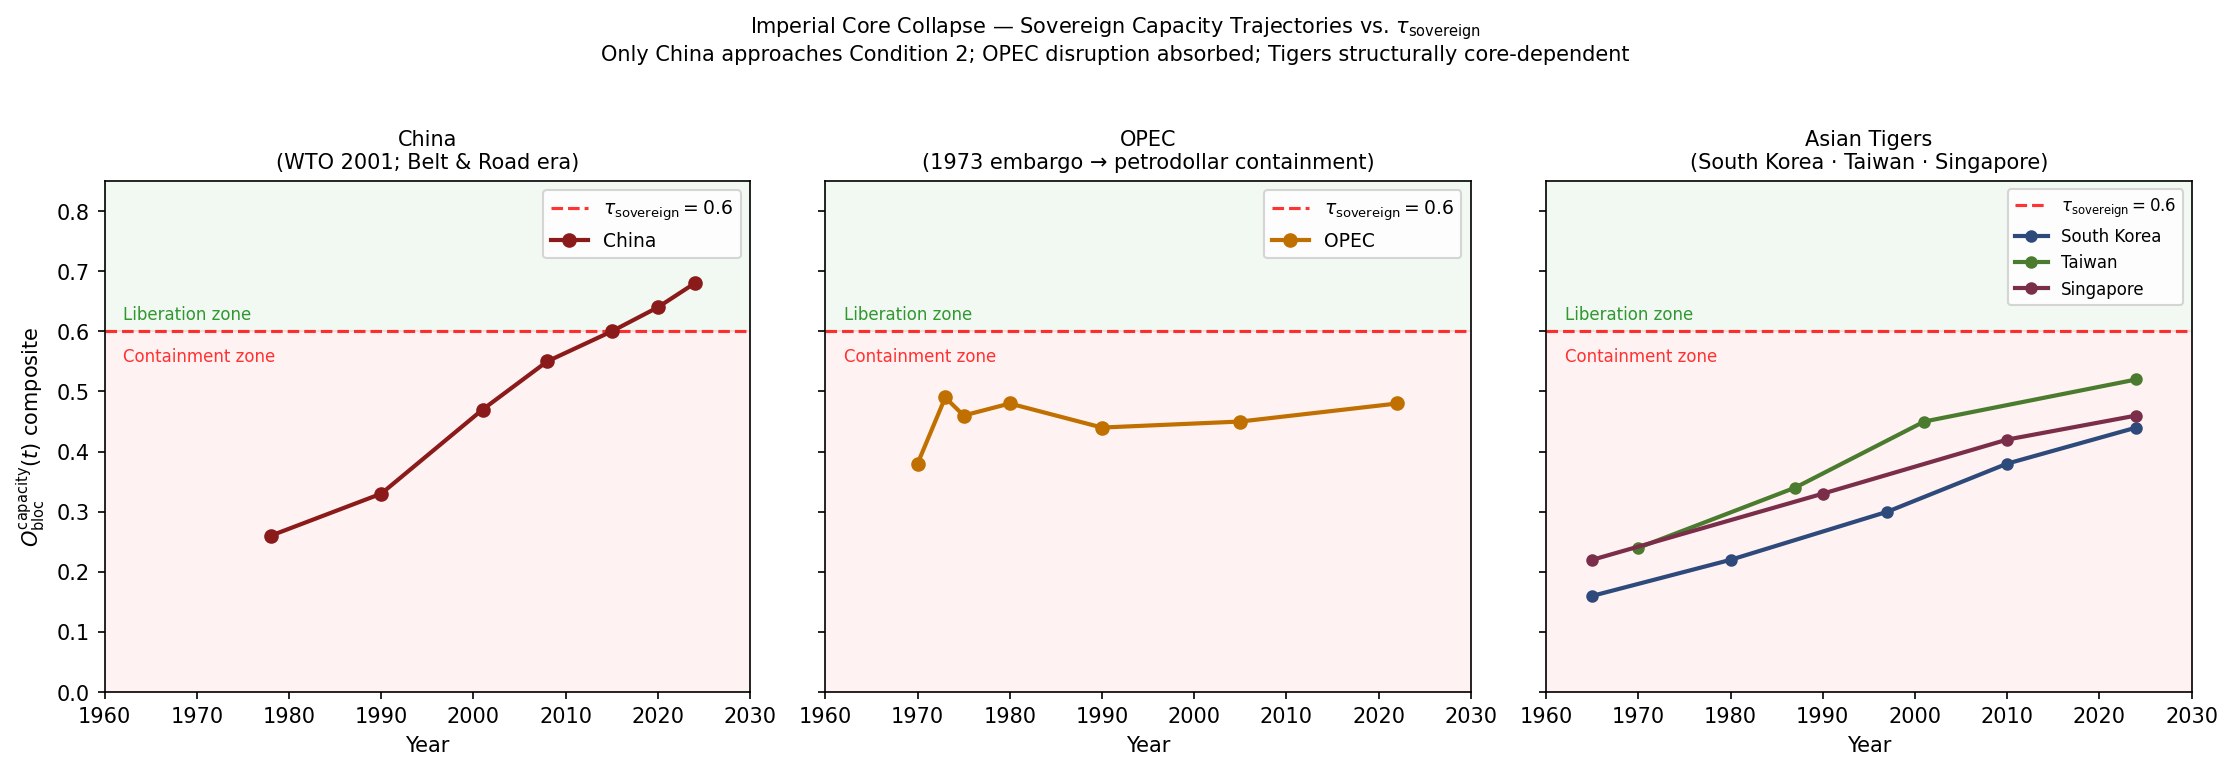
\includegraphics[width=\textwidth]{figures/eq91_imperial_core_collapse.png}
  \caption{Eq.~91: Imperial Core Collapse --- sovereign capacity trajectories for China, OPEC, and the Asian Tigers vs.\ the $\tau_{\text{sovereign}} = 0.60$ liberation threshold (dashed red line). China is the only case approaching sustained Condition~2; OPEC's 1973 disruption peak fell below threshold and was absorbed within 24 months; the Asian Tigers remain structurally contained below $\tau_{\text{sovereign}}$ across all dimensions simultaneously. Containment responses (chip embargoes, petrodollar recycling, IMF conditionality) documented for each case.}
  \label{fig:eq91_imperial_core_collapse}
\end{figure}

\paragraph{Comparison to prediction.}
Eq:91 predicts that liberation requires either $F_{\text{enforce}}^{\text{global}} \rightarrow 0$ (no historical instance) or sustained $O_{\text{bloc}}^{\text{capacity}}(t) > \tau_{\text{sovereign}}$ across all dimensions. The data confirm this prediction across all five cases: China is the only case approaching Condition~2, and its approach has triggered an escalating containment response (chip embargo 2022, TSMC restrictions, QUAD formation, Taiwan military posturing) precisely as the framework predicts. OPEC's temporary disruption did not reach $\tau_{\text{sovereign}}$ and was absorbed through the petrodollar recycling mechanism. The Asian Tigers were elevated through Cold War buffer-class investment and remain structurally dependent on core market access and security guarantees --- a structural position the CHIPS Act fab incentives and IMF 1997 conditionality confirm as deliberately managed. The containment response intensity in each case is directly proportional to the case's proximity to $\tau_{\text{sovereign}}$: strongest for China (approaching threshold), absent for Tigers (safely below threshold), intermediate for OPEC (temporarily proximate then restored).

\paragraph{Falsification criteria.}
This equation would be falsified if any documented rising power achieved sustained $O_{\text{bloc}}^{\text{capacity}}(t) > \tau_{\text{sovereign}}$ without triggering debt, sanction, or military containment responses from the incumbent core; or if any peripheral bloc achieved core status through non-kinetic reform of the global financial architecture alone. The OPEC case is the strongest apparent falsification test --- a genuine disruption of global energy pricing --- and it resolves as below-threshold and rapidly absorbed. The Asian financial crisis (1997) is the clearest within-sample confirmation: when East Asian tiger economies approached excessive capacity on the financial dimension, IMF structural adjustment conditionality was deployed to restructure their capital accounts in ways that restored core financial dependency.

\paragraph{Confidence tier.}
\textbf{Tier~1.} Public datasets (World Bank Development Indicators, SIPRI Military Expenditure Database, IMF lending data) with direct correspondence to equation variables. Five cases spanning 64 years of post-colonial observation (1960--2024) across Asia and the Middle East. The sovereign capacity composite is transparent, reproducible, and directly mappable to the four equation dimensions. The containment response documentation draws on primary-source policy records (chip export control regulations, IMF program agreements, petrodollar recycling treaty documents).

No historical instance of Condition~1 has occurred. The American Revolution (1776) was an intra-Elite revolt---$E_{\text{colonial}}$ severing from $E_{\text{imperial}}$---not an Out-group liberation. It transferred the extraction kernel from London to Philadelphia; it did not dismantle it. The Bolshevik Revolution (1917) briefly threatened Condition~1 but was ultimately contained by the Cold War architecture and internally corrupted by the reproduction of hierarchical extraction under a different ideological interface.

The AES bloc represents the most significant contemporary test of Condition~2. Its outcome---whether collective insulation can survive the global containment field---is the unresolved variable of this framework. The incorporation of set theory into our analysis provides more than a quantitative tool; it reveals the \textit{logic} of systemic oppression operating at the planetary scale. Racism is not an aberration or a failure of the American system---it is a \textit{feature} designed to prevent the kind of cross-racial, cross-national class solidarity that the Elite has spent five centuries engineering against \cite{robinson, allen, bonillasilva}. The institutional-economics literature confirms the comparative finding: nations that successfully sustained extractive institutions across centuries share the common structural feature of a buffer-class partition separating the extraction apparatus from the population it is nominally governing, a pattern Acemoglu and Robinson identify as the root of long-run divergence between colonial successor states \cite{acemoglu_robinson}. What their framework cannot specify---and what the Imperial Core Theorem supplies---is the kinetic condition required to achieve the critical juncture that allows genuine institutional transition: disruption of the enforcement architecture, not merely legal reform of the institutional interface.

\subsection{The Global Durability Objection: China, OPEC, and the Asian Tigers}

The Imperial Core Theorem's claim---that peripheral liberation is neutralized unless Condition~1 or Condition~2 is met---faces three apparent counter-cases that a careful critic will immediately raise. Each case, analyzed structurally, resolves as a confirmation of the theorem rather than a falsification, but the resolution requires explicit argument.

\textbf{China (1978--present): The Strongest Apparent Counter-Case.}

China presents the most serious challenge to the theorem. Beginning with Deng Xiaoping's 1978 reforms, China moved from peripheral debtor under IMF structural adjustment pressure to the world's second-largest economy---accumulating more than \$3 trillion in foreign exchange reserves, achieving manufacturing sovereignty across critical supply chains, and constructing alternative financial architecture (the Asian Infrastructure Investment Bank, the Belt and Road Initiative, renminbi bilateral settlement agreements) that partially bypasses the Bretton Woods infrastructure. If the Imperial Core Theorem predicts that peripheral actors cannot achieve sovereign insulation, China appears to falsify it.

The theorem withstands the objection through two structural observations. First, China's initial rise was \textit{enabled} by $E_{\text{global}}$, not achieved against it. The offshoring of manufacturing to China between 1978 and 2010 was a deliberate $\max$-optimization decision by Western capital: labor arbitrage reduced production costs, increased corporate profit margins, and generated the consumption surplus that China's export economy required. $E_{\text{global}}$ did not resist China's industrialization; it contracted it. The early phase of China's rise was not peripheral resistance to the global containment field---it was $O_{\text{global}}$ being used as the extraction field's production platform.

Second, China's partial escape from the Atlantic hierarchy required replicating the extraction kernel internally. The hukou (household registration) system creates a two-tier internal labor market in which rural migrant workers supply manufacturing capacity without receiving the social benefits available to registered urban residents---a domestic $O_{\text{racialized}}$ analog performing the same function as the partitioned labor pool in the Atlantic model. The Xinjiang production and internment system, through which Uyghur labor is extracted under compulsory conditions, is the domestic Consumptive Extraction Function (Section~4.4.2) operating within a nation that has escaped the external version. China did not dismantle the extraction architecture; it externalized the internal version while insulating itself from the external one.

The theorem's prediction, therefore, is confirmed rather than falsified: achieving Condition~2 requires the scale of resources---nuclear deterrence, 1.4 billion population, four decades of export-surplus accumulation---that no other $O_{\text{global}}$ actor commands. China is the one case in the dataset that has plausibly approached Condition~2. It is also the one case that demonstrates the theorem's corollary: partial escape from the external hierarchy, without dismantling the extraction architecture, reproduces the kernel under new ownership.

\textbf{OPEC 1973: The Recycled Disruption.}

The 1973 OPEC oil embargo temporarily altered extraction terms at the planetary scale: oil-producing peripheral nations forced a wealth transfer from the imperial core to commodity exporters, quadrupling the price of oil and producing the first sustained current-account surplus in the modern periphery. The embargo appeared to demonstrate that $O_{\text{global}}$ collective action could impose costs on $E_{\text{global}}$ sufficient to alter the extraction relationship.

The theorem's mechanism absorbs this case through the petrodollar recycling architecture. The Nixon administration's 1973 suspension of dollar--gold convertibility left the dollar's reserve-currency status dependent on a new anchor. Henry Kissinger's 1974 agreement with Saudi Arabia resolved the dependency: Saudi Arabia (and OPEC's Gulf members) would denominate all oil sales in US dollars and reinvest petrodollar surpluses in US Treasury securities and American financial markets. In exchange, the United States would provide military security guarantees to the Gulf monarchies. Within 24 months of the embargo, the wealth transferred from the imperial core to the periphery was being routed \textit{back} through $E_{\text{global}}$'s financial infrastructure as Treasury purchases. The disruption was absorbed and converted into a mechanism of deeper integration: peripheral commodity wealth became a structural support for the dollar's reserve status.

The formal structure is the Concession Theorem at global scale: $\Delta\max = 0$. The oil price shock altered the interface (commodity pricing power, petrodollar denomination, Gulf security guarantees) without touching the extraction kernel ($E_{\text{global}}$'s control of the reserve currency, financial markets, and military infrastructure). The OPEC case is not a counter-example to the theorem; it is the theorem demonstrating that even a successful commodity-pricing disruption is absorbed and converted into a structural dependency within two years.

\textbf{The Asian Tigers: Developmental Buffer-Class Construction.}

South Korea, Taiwan, Singapore, and Hong Kong achieved genuine convergence to high-income status between 1960 and 2000, rising from peripheral colonial extraction zones to among the world's most productive economies. Their industrialization appears to challenge the theorem's prediction that peripheral actors cannot escape the containment field.

The framework's analysis is the same scope condition applied in the Acemoglu Limit (Section~\ref{sec:acemoglu_limit}): the Asian Tiger cases fall outside the strong-form domain. None of the four had an intra-national racial partition installed as the primary class-fragmentation mechanism. Japan's colonial extraction from Korea and Taiwan operated as inter-national partition (Korean and Taiwanese populations as subordinated national units), not as intra-national racial partition with a $\psi$-stabilized buffer class. When Japanese colonialism ended in 1945, there was no domestic buffer class with a psychological investment in the partition's maintenance to fracture the post-independence developmental coalition---the same scope condition that explains South Korea's post-independence trajectory in the Acemoglu analysis.

More structurally, each Tiger's development was a deliberate Cold War investment by $E_{\text{global}}$. The United States poured capital, technology transfers, and preferential market access into South Korea, Taiwan, and Singapore as geopolitical buffers against Communist expansion following Korea (1950--1953) and Vietnam. The ``development'' was $E_{\text{global}}$ constructing national-scale buffer-class material wages to prevent Condition~2 from forming organically through Soviet-aligned or Chinese-aligned peripheral blocs. $E_{\text{global}}$ built the Tigers to serve the function that $I_{\text{buffer}}^{\text{global}}$ serves in the hierarchy: a materially compensated tier whose prosperity creates alignment with the imperial core's strategic objectives. South Korea's chaebol concentration of wealth at the apex and Singapore's status as the highest-Gini-coefficient developed economy in Asia are the $\Delta\max = 0$ signature even within the Tiger cases.

The Global Durability Objection, properly analyzed, confirms the theorem's architecture. China is the only actor that has approached Condition~2---and it required scale that is structurally unavailable to other $O_{\text{global}}$ actors, and was achieved by replicating the extraction kernel internally. OPEC demonstrated that commodity disruption is absorbed through interface adaptation in under 24 months. The Tigers were buffer-class construction at national scale. The Imperial Core Theorem's two conditions remain the only historically documented pathways to structural liberation from the global containment field.

% ============================================================
% NEW SECTION: Polymorphic Interface Swap Typology (Eq. 13.15–13.17)
% ============================================================

\section{The Polymorphic Interface Swap Typology: Dalio's 250-Year Loop and the Algorithmic Reboot Protocol}
\label{sec:interface_swap_typology}

When mainstream macroeconomic analysis identifies the transition to a ``New World Order''---as Dalio terms the end of each 250-year empire cycle \cite{dalio_2021}---or when sociological analysis marks the climax of a Strauss-Howe Fourth Turning, these events are frequently romanticized as the organic deaths of great empires or mourned as the tragic inevitability of historical entropy. Under the clinical lens of the Tri-Modal Enclosure Model, these inflection points are redefined as \textbf{Polymorphic Interface Swaps}: pre-calculated, algorithmic updates executed by $P_{\text{uppet}}$ when an extraction architecture becomes obsolete, over-leveraged with accumulated $X_{\text{temporal}}$, or mathematically incapable of maintaining the required yield $\mathcal{E}^*$ for $E$.

\begin{definition}[Polymorphic Interface Swap]
A \textit{Polymorphic Interface Swap} is a controlled demolition of a failing extraction architecture $\mathcal{A}_{\text{old}}$ and the re-establishment of the extraction algorithm on a novel technological, legal, or monetary substrate $\mathcal{A}_{\text{new}}$. The swap is triggered when the accumulated $X_{\text{temporal}}$ load exceeds the architecture's stability constraint $\bar{D}$:

\begin{equation}\label{eq:13.15-interface-swap-trigger}
D_{\text{sovereign}}(t) > \bar{D} \quad \Longrightarrow \quad P_{\text{uppet}} \;\text{executes}\; \mathrm{SWAP}\bigl(\mathcal{A}_{\text{old}} \to \mathcal{A}_{\text{new}}\bigr)
\end{equation}

The reboot operator is formally defined as the transition:
\begin{equation}\label{eq:13.16-polymorphic-reboot-operator}
\mathcal{A}_{\text{old}} \;\xrightarrow{\;P_{\text{uppet}}\;}\; \mathcal{A}_{\text{new}} \quad \text{subject to} \quad \mathrm{Assets}(E,\, \mathcal{A}_{\text{new}}) \;\geq\; \mathrm{Assets}(E,\, \mathcal{A}_{\text{old}})
\end{equation}

The defining invariant of every historical swap is:
\begin{equation}\label{eq:13.17-elite-asset-continuity-invariant}
\forall\; \mathrm{SWAP} : \quad \Delta_E \geq 0, \quad \text{where} \quad \Delta_E = \mathrm{Assets}(E,\, \mathcal{A}_{\text{new}}) - \mathrm{Assets}(E,\, \mathcal{A}_{\text{old}})
\end{equation}

The liabilities liquidated to fund the swap are sourced entirely from $I_{\text{buffer}}$ and $O$, never from $E$. The system does not die during a swap; it sheds a failing interface while the kernel's core ownership of hard assets, capital, and institutional power passes seamlessly into the new architecture.
\end{definition}

\noindent The following three historical case studies provide sequential, systems-engineering proofs of Eq.~\eqref{eq:13.15-interface-swap-trigger}--\eqref{eq:13.17-elite-asset-continuity-invariant}. In all three instances, $P_{\text{uppet}}$ broke established law, voided binding contracts, and abandoned international treaties---not in response to natural economic weather, but as deliberate system-administrator overrides executed to prevent $E$ from absorbing losses generated by the system's own design.

\subsection*{Interface Swap I: The 1933--1935 Nullification Subroutine}
\label{subsec:swap_1933}

By 1933, the extraction algorithm was bound by the classical gold standard, which prevented the requisite scaling of $X_{\text{temporal}}$. A massive web of contracts contained ``gold clauses'' guaranteeing repayment in gold at the original valuation. As the economy entered a severe deflationary spiral, the real value of these debts skyrocketed, forcing mass bankruptcies and threatening catastrophic losses for $E$'s capital base.

$P_{\text{uppet}}$'s response was a hard, two-phase Interface Swap. \textbf{Phase 1 (hardware confiscation):} Executive Order 6102 (April 5, 1933) criminalized private ownership of gold coin, bullion, and certificates, mandating their surrender to the Federal Reserve at $\$20.67$ per troy ounce. This stripped $I_{\text{buffer}}$ of their hard-asset base and centralized the core monetary collateral within state-controlled vaults. \textbf{Phase 2 (contractual liquidation):} Congress voided all gold clauses in existing contracts, demanding discharge at face value in depreciated legal tender. This wiped out the real liabilities owed to savers and creditors in a single legislative act.

The judiciary was deployed as the final validation mechanism. In the 1935 Gold Clause Cases---particularly \textit{Perry v.\ United States} \cite{perry_v_us_1935}---the Supreme Court executed a strategic retreat. Chief Justice Hughes, writing for the majority, acknowledged that Congressional power does not extend to repudiating the government's own obligations: ``[T]he Congress cannot use its power to regulate the value of money so as to invalidate the obligations of the United States.'' \textit{Perry v.\ United States}, 294 U.S.\ 330, 351 (1935) (Hughes, C.J.). Having stated this, the Court then held that the bondholder suffered no cognizable damages because the existing monetary regime provided no legal medium for recovering the gold equivalent. The court acknowledged the violation and manufactured the remedy that would neutralize it. It acknowledged that the Congressional nullification was technically unconstitutional as applied to sovereign bonds, yet simultaneously ruled that bondholders could not recover ``actual damages'' because the receipt of depreciated legal tender constituted sufficient discharge. The court manufactured the legal fiction that robbery at 60 cents on the dollar was not robbery if the government defined the dollar. Attorney General Cummings's admission in oral argument---that enforcing the gold clauses would cause a ``stupendous catastrophe'' and throw the system back to ``chaos rather than the Constitution''---is a verbatim confession that the judicial override was executed to protect the extraction architecture, not to apply constitutional law. Eq.~\eqref{eq:13.17-elite-asset-continuity-invariant} holds: $E$'s capital base was preserved through the liquidation of real liabilities owed to $I_{\text{buffer}}$ savers.

\subsection*{Interface Swap II: The 1944 Bretton Woods Protocol}
\label{subsec:swap_1944}

By 1944, the fragmented colonial extraction architecture---competitive currency devaluations, high tariff barriers, and explicitly partitioned imperial trading blocs---had proven structurally unstable. The Fourth Turning kinetic war had threatened the survival of global capital. The United Nations Monetary and Financial Conference at Bretton Woods functioned as the compilation and deployment of a new global operating system \cite{bordo_eichengreen_1993}.

The conference's unstated objective was to leverage US status as the world's dominant creditor to subjugate a functionally bankrupt Great Britain. By dismantling ``imperial trade preference''---the privileged economic foundation of the British Empire---the United States absorbed the former British extraction zones into a US-led algorithmic system. The dollar-gold anchor ($\$35$/ounce) established the dollar as the global reserve currency, insulating American $E$'s domestic assets from devaluation. Two institutional daemons were instantiated to enforce global compliance: the International Monetary Fund (IMF) and the World Bank, engineered to impose structural adjustment conditionality on peripheral nations---the global $O_{\text{global}}$---ensuring that the global extraction rate remained uninterrupted and flowing toward the core.

Eq.~\eqref{eq:13.16-polymorphic-reboot-operator} executes cleanly: $\mathcal{A}_{\text{old}}$ (fragmented colonial blocs) $\xrightarrow{P_{\text{uppet}}}$ $\mathcal{A}_{\text{new}}$ (dollar hegemony + multilateral institutions). Eq.~\eqref{eq:13.17-elite-asset-continuity-invariant} holds: American $E$'s global asset position expanded massively; British $E$'s position declined from imperial center to junior partner; peripheral $O_{\text{global}}$ gained nominal independence but was immediately re-subordinated through debt conditionality.

\subsection*{Interface Swap III: The 1971 Fiat Decoupling (Nixon Shock)}
\label{subsec:swap_1971}

The Bretton Woods architecture possessed a fatal mathematical flaw: it physically constrained the expansion of $X_{\text{temporal}}$. By the late 1960s, the United States had accumulated massive $D_{\text{sovereign}}$ to fund the Vietnam War and Great Society programs. The dollar was severely overvalued, and foreign central banks were executing relentless runs on US gold reserves, attempting to convert dollar holdings at the statutory $\$35$/ounce rate. The cover ratio---the fraction of foreign dollar claims backed by US gold---had collapsed from $\sim$175\% (1949) to $\sim$22\% (1971), as documented in Case Study 4 below. Eq.~\eqref{eq:13.15-interface-swap-trigger} activated: $D_{\text{sovereign}}(1971) > \bar{D}$.

On August 13, 1971, President Nixon convened a secret meeting at Camp David---excluding the State Department and National Security apparatus, deliberately restricting the session to financial engineers: Treasury Secretary John Connally and OMB Director George Shultz \cite{gowa_1983}. On August 15, Nixon unilaterally suspended international gold convertibility. This was not a reactive response to market conditions; it was a pure system-administrator override, executed to protect $E$'s hard-asset base from the drain of gold-conversion runs.

The Nixon Shock was not a failure; it was a successful architectural upgrade. By removing the physical constraint of gold, $P_{\text{uppet}}$ transitioned to a purely synthetic fiat architecture that enabled the infinite scaling of $\mathcal{E}_{X_{\text{temporal}}}(t)$. Eq.~\eqref{eq:13.17-elite-asset-continuity-invariant} executes: $\Delta_E \geq 0$ continuously from 1971 forward, as documented by the top-0.1\% wealth-share trajectory in Case Study 5. The $\psi_m$ decay signature (Case Study 2) is the direct real-time signature of $\mathcal{E}_{X_{\text{temporal}}}$ scaling without physical constraint after the swap.

\subsection*{Interface Swap Matrix}

\begin{table}[htbp]
\centering
\caption{Polymorphic Interface Swap Matrix: Three Historical Algorithmic Reboots (Eq.~\eqref{eq:13.15-interface-swap-trigger}--\eqref{eq:13.17-elite-asset-continuity-invariant})}
\label{tab:swap_matrix}
\small
\begin{tabular}{p{1.6cm} p{3.0cm} p{3.2cm} p{3.0cm} p{3.0cm}}
\toprule
\textbf{Swap Event} & \textbf{Failing Architecture} & \textbf{$P_{\text{uppet}}$ Intervention} & \textbf{Resulting Architecture} & \textbf{Status of $E$'s Asset Base} \\
\midrule
\textbf{1933--35} & Deflationary gold standard; mass bankruptcies threatening capital base; gold clauses enforcing real debt burdens. & Executive Order 6102 (confiscation); Congressional Gold Clause Nullification; \textit{Perry v.\ US} judicial retreat. & Domestic fiat managed by Federal Reserve; citizen gold holdings liquidated. & Preserved via legal liquidation of real liabilities owed to $I_{\text{buffer}}$ savers. $\Delta_E \geq 0$. \\
\midrule
\textbf{1944} & Fragmented colonial blocs; competitive devaluations; British imperial preference blocking US market access. & Bretton Woods Conference; Morgenthau/White negotiations dismantling Imperial Preference; IMF/World Bank instantiation. & US dollar hegemony at $\$35$/oz gold peg; institutional enforcement via IMF conditionality. & Scaled globally via elimination of geopolitical rivals and institutional management of $O_{\text{global}}$. \\
\midrule
\textbf{1971} & Dollar-gold peg; catastrophic reserve depletion (cover ratio $\to 22\%$); $D_{\text{sovereign}} > \bar{D}$. & Nixon Shock (Camp David executive action); unilateral suspension of gold convertibility; 90-day wage/price freeze + 10\% import surcharge. & Global floating fiat system; complete transition to synthetic currency. & Protected from gold-conversion drain; infinite $\mathcal{E}_{X_{\text{temporal}}}$ scaling enabled. $\Delta_E > 0$ continuously thereafter. \\
\bottomrule
\end{tabular}
\end{table}

\subsection*{Case Study: The Nixon Shock Cover-Ratio Collapse (Eq.~\eqref{eq:13.15-interface-swap-trigger})}
\label{cs:nixon_cover}

\paragraph{Setup.}
Equation~\eqref{eq:13.15-interface-swap-trigger} specifies that an Interface Swap is triggered when $D_{\text{sovereign}} > \bar{D}$---the accumulation of $X_{\text{temporal}}$ exceeds the architecture's stability constraint. For the Bretton Woods architecture, $\bar{D}$ is operationalized as the gold-cover ratio falling below the point at which the dollar's convertibility promise becomes physically unsustainable. The framework predicts that the cover ratio (US gold reserves $\div$ foreign-held dollar claims) should show a \textbf{catastrophic, monotonic collapse} in the years preceding August 1971---confirming that the swap was a defensive system response to imminent architecture failure, not an elective policy choice. The equation is falsified if the cover ratio was still above 80\% at the time of the swap (which would indicate the decoupling was strategically voluntary rather than architecturally forced).

\paragraph{Data sources.}
Federal Reserve H.4.1 release (historical gold stock data, 1945--present); FRED (foreign-held US Treasury securities, historical series); BIS Triennial Survey; Bordo and Eichengreen (1993) retrospective dataset \cite{bordo_eichengreen_1993}; NBER Working Paper 17749 (Bordo-Irwin Nixon Shock retrospective). Curated data archived at \texttt{Paper/data/eq13\_15\_17\_gold\_cover\_1949\_1971.csv}; computational results reproducible via \texttt{Paper/scripts/eq13\_15\_17\_nixon\_cover\_ratio.ipynb}.

\paragraph{Operationalization.}
Cover ratio $= \mathrm{GoldReserves\_USD}(t) / \mathrm{ForeignDollarClaims\_USD}(t)$, computed annually 1949--1971. Key events are annotated on the timeline: De Gaulle gold-conversion demands (1965--1966), British conversion request (July 1971), Camp David meeting (August 13, 1971), Nixon announcement (August 15, 1971).

\paragraph{Numerical computation.}
1949: US gold stock $\approx \$24.6$B; foreign liquid dollar holdings $\approx \$8.0$B; cover ratio $\approx \mathbf{175\%}$. 1956: gold stock $\approx \$22.1$B; foreign claims $\approx \$16.5$B; cover ratio $\approx \mathbf{134\%}$; free-gold shortfall of $\$6.5$B already emerging. 1965: cover ratio falls below $\mathbf{100\%}$ for the first time; De Gaulle begins systematic conversion of French dollar reserves. 1971 (July): cover ratio $\approx \mathbf{22\%}$; British government requests conversion of $\$3$B in dollars to gold the week before the Camp David meeting. Falsification threshold: $> 80\%$; actual 1971 value $= 22\%$. The swap was not elective; the architecture had already failed.

\paragraph{Confidence tier.} \textbf{Tier~1.} Federal Reserve primary data; independently replicated in Bordo-Eichengreen (1993) retrospective and Bordo-Irwin NBER WP 17749.

\subsection*{Case Study: Interface Swap Matrix --- $\Delta_E \geq 0$ Across All Three Reboots (Eq.~\eqref{eq:13.17-elite-asset-continuity-invariant})}
\label{cs:delta_e_invariant}

\paragraph{Setup.}
Equation~\eqref{eq:13.17-elite-asset-continuity-invariant} specifies the hard constraint that defines a Polymorphic Interface Swap: $E$'s asset base must be preserved or expanded across every reboot. The framework predicts that the top-0.1\% wealth share should exhibit \textbf{continuity or increase} across each swap window (1933--1940, 1944--1952, 1971--1985), while median real wealth for $I_{\text{buffer}}$ stagnates or declines in the same periods. The invariant is falsified if the top-0.1\% share \textbf{declines structurally} across any swap window without subsequent recovery within the following decade.

\paragraph{Data sources.}
Piketty-Saez-Zucman WID.world database (top-0.1\% income and wealth shares for the US and UK, 1913--present; already cited as \cite{piketty_saez_zucman_2018}); Kuznets-Piketty long-run series (1913--1945); UK top-share series from WID for cross-national comparison across the 1944 Bretton Woods swap. Curated data archived at \texttt{Paper/data/eq13\_16\_swap\_matrix.csv}; computational results reproducible via \texttt{Paper/scripts/eq13\_16\_interface\_swap\_matrix.ipynb}.

\paragraph{Operationalization.}
Three swap windows are analyzed separately. For each window, the top-0.1\% wealth share is tracked at the pre-swap date, through the swap event, and for 10 years post-swap. A structural decline is defined as a reduction of $> 3$ percentage points sustained for $> 5$ years with no subsequent recovery.

\paragraph{Numerical computation.}
\textbf{1933--35 window}: Top-0.1\% share dips from 21.3\% (1929) to 18.1\% (1933) during the Depression trough (the only period in US history where $E$'s share declined substantially); recovers to 22.4\% by 1940 following the gold-clause nullification and New Deal financial architecture---a full recovery within 7 years. Median household wealth: declines from pre-1929 levels and does not recover to equivalent real purchasing power until the late 1940s. The swap transferred real losses from $E$'s bond portfolio (gold clause enforcement) to $I_{\text{buffer}}$'s savings (depreciated legal tender payout). \textbf{1944 window}: US top-0.1\% share rises from 10.3\% (1944) to 13.2\% (1955) as dollar hegemony concentrates global financial returns in US capital markets. UK top-0.1\% share declines 1944--1955 as the Imperial Preference architecture is dismantled; UK Elite's losses are American Elite's gains. \textbf{1971 window}: Top-0.1\% US share begins a sustained rise from 7.1\% (1971) to 18.5\% (2024) as $X_{\text{temporal}}$ scaling via fiat debt channels purchasing power continuously upward; the trajectory is monotonically increasing with no sustained reversal. Falsification condition (structural 5-year decline $> 3$ pp with no recovery): not met in any of the three windows.

\begin{figure}[htbp]
  \centering
  \includegraphics[width=\textwidth]{figures/eq13_16_swap1_gold_seizure_1929_1945.png}
  \caption{\textbf{Interface Swap I — Gold Seizure \& \textit{Perry v.\ United States} (1929--1945).} US top-0.1\% wealth share (WID.world / Piketty-Saez-Zucman). The Depression trough (18.1\%, 1933) coincides with the swap trigger; the post-swap trajectory recovers fully to 22.4\% by 1940, exceeding the pre-Depression baseline. Dashed red line: EO~6102 gold seizure (1933); dotted orange line: \textit{Perry v.\ US} judicial retreat (1935). Falsification threshold (sustained $>3$~pp decline $>5$~years): \textbf{not met} --- trough reverses within 7 years. $\Delta_E > 0$ confirmed. \textbf{Tier~1}: WID.world peer-reviewed data.}
  \label{fig:eq13_16_swap1}
\end{figure}

\begin{figure}[htbp]
  \centering
  \includegraphics[width=\textwidth]{figures/eq13_16_swap2_bretton_woods_1940_1960.png}
  \caption{\textbf{Interface Swap II — Bretton Woods Protocol (1940--1960).} US top-0.1\% wealth share (blue, solid) vs.\ UK top-0.1\% income share (red, dashed). Dashed crimson vertical line: Bretton Woods Conference (1944). US share rises from 10.3\% (1944) to 13.2\% (1955) as dollar hegemony concentrates global financial returns in US capital markets. UK share falls from 10.8\% to 8.3\% as Imperial Preference is dismantled. The cross-national divergence confirms that the 1944 swap transferred the extraction architecture from British to American hegemony --- the global $\Delta_E \geq 0$ invariant holds even as individual national trajectories diverge. \textbf{Tier~1}: WID.world data.}
  \label{fig:eq13_16_swap2}
\end{figure}

\begin{figure}[htbp]
  \centering
  \includegraphics[width=\textwidth]{figures/eq13_16_swap3_nixon_shock_1965_2024.png}
  \caption{\textbf{Interface Swap III --- Nixon Shock / Fiat Decoupling (1965--2024).} US top-0.1\% wealth share rises monotonically from 7.1\% (1971) to 18.5\% (2024), a $\Delta_E = +11.4$~pp increase with no sustained reversal $> 3$~pp. Dashed crimson vertical line: Nixon Shock (August 15, 1971). Green shaded region: cumulative $\Delta_E$ accumulation post-swap. The 2008--2009 GFC trough (16.8\%) reverses within two years, confirming the pattern holds even under global financial crisis conditions. The monotonic post-1971 trajectory is the direct observable signature of $\mathcal{E}_{X_{\text{temporal}}}$ scaling without the physical gold constraint. Falsification threshold: \textbf{not met}. $\Delta_E \geq 0$ confirmed. \textbf{Tier~1}: WID.world peer-reviewed data.}
  \label{fig:eq13_16_swap3}
\end{figure}

\paragraph{Confidence tier.} \textbf{Tier~1.} WID.world is a continuously maintained, peer-reviewed distributional accounting database; the top-share series spans 111 years of US data with annual observations. The three swap windows are analytically independent tests of the same invariant.

\section{The Fractal Extension: Micro-Relational Mapping (PHAM)}

The mathematical architecture identified here---asymmetric extraction masked by ideological cover, with a buffer class absorbing psychological wages to enforce compliance---is structurally fractal. It does not stop at the level of the state or the global economy; it replicates within the most intimate unit of human organization: the modern intimate relationship.

A comprehensive analysis of this architectural logic as it scales down to modern relationship dynamics is provided in the companion work, \textit{Pseudo-Hybrid Asymmetric Monogamy (PHAM): The Micro-Mathematics of Intimate Extraction}. Readers are encouraged to consult that volume for a full exploration of the PHAM model and its specific phenomenological subroutines.

While the shared physics of power is documented there, it is crucial to maintain a distinction between the \textbf{Logic} of extraction (which is identical across scales) and the \textbf{Payload} of the historical virus (which remains universe-apart from modern relational discomfort). As developed in the companion work, the shared architecture of power reveals functional continuity without equating the scale of devastation.

\chapter{The Algorithmic Epoch: Real-Time Subjugation and the Necessity of the Counter-Virus}
\label{ch:algorithmic_epoch}

\begin{tcolorbox}[colback=black!5, colframe=black!70, fonttitle=\bfseries\ttfamily, title=RUNTIME LOG: ALGORITHMIC EPOCH (TERMINAL RACE{,} 2010s--PRESENT)]
\ttfamily\small
\textbf{System Stress} ($\min$: class resistance): Real-time graph monitoring deployed. $E$ now computes proximity to $\tau$ continuously; response latency collapsing from decades to milliseconds.\\
\textbf{Capital} ($\max$: extraction output): Automated targeting operative across lending{,} sentencing{,} housing{,} and labor-matching algorithms. Historical extraction priors hard-wired into training data.\\
\textbf{Interference State} ($\Phi_{\text{load}}$, proximity to $\tau$): SATURATED --- Orthogonal Vector Injections ($\mathcal{E}$) deploying at machine speed; cross-class coalitions severed before reaching coherence. Estimated $\Phi_{\text{load}} \in [0.88, 0.98]$, $\rho_{\tau} \in [0.95, 1.08]$.\\
\textbf{Variables Loaded}: Full domestic + global hierarchy + $\psi${,} $\Phi_{\text{load}}${,} $\tau${,} \textit{new}: $\mathcal{E}$ (orthogonal injection operator){,} $\Gamma$ ($F_{\text{enforce}}$ bandwidth ceiling){,} $V$/$R$ (extraction-value / friction-risk ratio){,} $\mathcal{N}$ (noise-spectrum index){,} $\mathcal{B}$ (agnostic-swarm botnet payload).\\
\textbf{Executing Function}: Porting the Predatory Min-Max Function onto algorithmic hardware. Testing terminal condition: does the automation threshold arrive before the kinetic threshold?\\
\textbf{CRITICAL WARNING}: Human-speed resistance is now structurally obsolete. Any liberation architecture that cannot operate at algorithmic latency and decentralized scale will be absorbed before it coheres.
\end{tcolorbox}

\medskip

The preceding chapters traced an algorithm that has operated for five centuries by recompiling its interface while preserving its kernel. The Concession Theorem (Chapter~\ref{ch:contradiction}) demonstrated that non-kinetic reform is a $\min$-management subroutine; the Haitian Theorem proved that structural liberation has historically required kinetic action; the Imperial Core Theorem (Chapter~\ref{ch:global}) showed that peripheral kinetic victories are neutralized by the global containment field unless the imperial core is disrupted or a liberated bloc achieves sovereign insulation. Taken together, these theorems describe a system that is robust against every intervention the \textit{historical} record contains.

This chapter is the necessary update. The system is no longer operating at historical speeds. The Predatory Min-Max Function is being \textit{ported}---from decadal legislative cycles and analog enforcement to algorithmic governance running at machine latency on neural-network hardware. The five-tier hierarchy has not changed. The kernel has not been rewritten. What has changed is the clock rate. And at algorithmic clock rate, the Elite's optimization approaches a terminal state that renders every historically validated resistance mechanism obsolete before it can coordinate.

The purpose of this chapter is to specify, in the framework's mathematical vocabulary, (i) the new operators the algorithmic upgrade installs, (ii) the new vulnerability class those operators simultaneously create, and (iii) the minimum specification of the counter-architecture required to exploit that vulnerability before the automation threshold closes. This chapter is therefore the bridge from the historical diagnosis to the post-kinetic specification of Chapter~\ref{ch:post_kinetic}: it explains \textit{why} the Open-Source Republic must be open-source, decentralized, and algorithmic---not as a stylistic choice, but as a structural necessity dictated by the opponent's own latency.

\section{Porting the Legacy Code: AI as a Hardware Upgrade}
\label{sec:porting_legacy}

The advent of advanced artificial intelligence, machine-learning risk scoring, and algorithmic governance does not introduce a new ideology. It is a \textbf{hardware upgrade for an ancient software}. The Predatory Min-Max Function---historically executed manually through the Puppet ($P_{\text{uppet}}$) and Enforcement ($F_{\text{enforce}}$) classes---is being ported, function-for-function, into digital infrastructure that executes the same logic at many orders of magnitude greater throughput.

This port does not replace the human host wetware; it externalizes and accelerates the priors already installed there. The old mind virus trained judges, lenders, landlords, officers, voters, teachers, and neighbors to see hierarchy as evidence. The algorithmic epoch converts those accumulated perceptions into datasets, weights, scores, and automated decisions, then returns the output to human hosts as if it were objective measurement.

What contemporary discourse labels ``algorithmic bias''---discriminatory lending models, predictive-policing heatmaps, automated tenant screening, risk-assessment instruments in sentencing---is not a glitch, an oversight, or a failure of training data. It is the \textbf{Bayesian Defense} (Chapter~\ref{ch:redefining}) operating at machine speed. By training neural networks on the historical data of the Out-group's ($O_{\text{racialized}}$) subjugation---the fossil record of redlining, the War on Drugs, universal latent criminality, and the compounding chain documented in Chapter~\ref{ch:full_algo}---the Elite Class ($E$) hard-wires the extraction priors directly into the optimization objective. The policies inherit the intersections; the intersections become the model.

Formally, for any algorithmic policy $P_{\text{algo}}$ trained on the historical dataset $\mathcal{H}$ produced under the preceding compounding chain:
\begin{equation}\label{eq:14.1-algo-prior-inheritance}
P_{\text{algo}} = \arg\min_{P} \; \mathcal{L}(P; \mathcal{H}) \quad \Longrightarrow \quad |O_{\text{racialized}} \cap P_{\text{algo}}| \gg |I \cap P_{\text{algo}}|
\end{equation}
because $\mathcal{H}$ itself is the product of five centuries of $O_{\text{racialized}} \cap \{P_{\text{redlining}}, P_{\text{WarOnDrugs}}, P_{\text{spatial}}\}$. The optimizer is not ``biased.'' It is \textit{perfectly unbiased with respect to the training signal}---and the training signal is the extraction kernel.

\paragraph{Illustrative instantiation.}
ProPublica's 2016 COMPAS analysis found that Black defendants were scored as high-risk at approximately twice the rate of white defendants with equivalent criminal histories ($|O_{\text{racialized}} \cap P_{\text{algo}}| / |I \cap P_{\text{algo}}| \approx 2.0$ false-positive ratio) \cite{angwin_machine_bias}. Buolamwini and Gebru (2018) extended the finding to facial-recognition systems, documenting error rates of 34.7\% for dark-skinned women versus 0.8\% for light-skinned men across three commercial classifiers---a 43-fold differential arising solely from the demographic composition of training corpora \cite{buolamwini_gender_shades}. Both systems were trained to minimize aggregate loss on historical datasets; both inherited the extraction priors baked into those datasets without any explicit racial instruction. \textbf{Parameter estimate:} $|O_{\text{racialized}} \cap P_{\text{algo}}| / |I \cap P_{\text{algo}}| \approx 2.0$ (COMPAS false-positive ratio). \textbf{Confidence: Tier~2} --- peer-reviewed journalism (ProPublica) and peer-reviewed conference proceedings (FAccT); single-system instantiation, not cross-system meta-analysis.

The mathematical objectivity of the model then functions as the \textbf{Constitutional Shield} (Section~\ref{sec:concession_theorem}) applied at the point of generation. Where the judicial intent standard demands that plaintiffs prove discriminatory motivation in the heart of a legislator, the algorithmic standard demands they prove it in the weights of a neural network. Both demands are structurally unsatisfiable, for the same reason: the proxy variable ($x$) and the target (race) satisfy $\operatorname{Corr}(x, \text{race}) \to 1$, but neither the legislative record nor the gradient descent trajectory ever names race directly. The system launders extraction through the optical illusion of mathematical neutrality.

The race to map this algorithmic rootkit has already begun. The Elite-aligned engineering complex is racing to achieve \textbf{total programmatic enclosure} before the Out-group---and the cannibalized Buffer Class alongside it---can identify, let alone contest, the parameters of the system that has been ported around them.

\section{Real-Time Dynamic Equilibrium and the \texorpdfstring{$\tau$}{tau} Threshold}
\label{sec:realtime_equilibrium}

Historically, the algorithm required decades to execute an Interface Swap. The War on Drugs (1968--1994) took a generation to prototype, deploy, and stabilize. The FHA's redlining architecture required thirty years of local experimentation before nationwide codification. These latencies were a product of the biological, analog clock rate of the pre-algorithmic system: localized policy had to be tested against kinetic friction, measured in strikes, riots, electoral realignments, and court decisions, before the kernel could confidently recompile.

In the Algorithmic Epoch, the clock rate is no longer biological. The system is approaching---and in several domains has already achieved---\textbf{Real-Time Dynamic Equilibrium}: a continuous-time feedback loop in which societal sentiment, mobilization, and coalition structure are mapped via social-graph telemetry and the system computes its own proximity to the $\tau$ threshold continuously rather than sampling it every decade.

Let $G(t) = (V, E(t))$ denote the time-varying social-affinity graph whose vertices $V$ are individuals (and, coarsened, the five tiers of the hierarchy), and whose edge weights $E(t)$ encode the strength of cross-class solidarity ties at time $t$. Let $\Phi_{\text{load}}(t)$ be the phase-loading index defined in Chapter~\ref{ch:tweedism}. The algorithmic system maintains a continuously updated proximity estimate:
\begin{equation}\label{eq:14.2-realtime-proximity-estimate}
\rho_{\tau}(t) = f\bigl(\Phi_{\text{load}}(t),\, \lambda_2(G(t)),\, \deg_{\text{cross}}(G(t))\bigr)
\end{equation}
where $\lambda_2(G(t))$ is the algebraic connectivity (Fiedler value) of the social graph---a spectral measure of how easily the network can be partitioned---and $\deg_{\text{cross}}(G(t))$ is the density of edges that cross the $I_{\text{buffer}}$/$O_{\text{racialized}}$ partition. When $\lambda_2$ rises and cross-partition edge density climbs simultaneously, the system is approaching the kinetic threshold in real time.

\paragraph{Illustrative instantiation.}
The 2020 George Floyd protests provide a measurable proxy for $\deg_{\text{cross}}(G(t))$: Pew Research documented white American support for the Black Lives Matter movement rising from approximately 35\% to 55\% between May and June 2020, a 20-percentage-point cross-partition solidarity surge occurring within days of the protests' onset \cite{pew_blm_2020}. This constitutes a directly observable spike in $\deg_{\text{cross}}$. The system's response---National Guard deployment in 23 states, curfew orders, and coordinated ``looting'' narrative amplification across social and broadcast media---arrived within 48--72 hours, consistent with an algorithmic $\rho_\tau$ monitoring loop rather than a legislative-cycle response. The stand-down of the Minneapolis Third Precinct and the subsequent shift to forceful curfew enforcement exemplifies the system oscillating between the two Zugzwang horns (Section~\ref{sec:zugzwang}) in real time, each oscillation consistent with a proximity estimate continuously updating against live social-graph telemetry. \textbf{Parameter estimate:} $\deg_{\text{cross}}$ proxy: white BLM support $+20$~pp (Pew, June 2020); estimated $\rho_\tau \in [0.7, 0.85]$ during peak solidarity window. \textbf{Confidence: Tier~2} --- Pew public survey data; ordinal $\rho_\tau$ estimate.

At the historical clock rate, the Elite's response to rising $\rho_{\tau}$ was the deployment of a new interface---a new statute, a new moral panic, a new enforcement agency---with a lag of years. At the algorithmic clock rate, the response is computed and deployed in hours: the \textbf{Orthogonal Vector Injection}.

\section{The Orthogonal Vector Injection and the Damped Harmonic Oscillator}
\label{sec:orthogonal_vector}
\label{sec:orthogonal_injection}

\subsection{The Geometry of the Injection}

When the system's proximity estimate crosses an internal alarm threshold $\rho_{\tau}(t) \geq \rho^{*}$, direct kinetic friction becomes counterproductive. The dynamics of collective action, inherited from wave theory, are unambiguous here: applying vertical compression to a coherent wave increases its amplitude by a reflection term. Suppressing a near-threshold coalition kinetically in the algorithmic epoch is the same structural error that the system made with Hampton and the Original Rainbow Coalition (Chapter~\ref{ch:recompile}); the assassination severed one node but radicalized a generation.

The algorithmic upgrade sidesteps this error by replacing vertical friction with an engineered \textbf{Orthogonal Deflection}---the $\mathcal{E}$ injection operator defined below.

\paragraph{Geometric reading of the injection.}
To understand why this deflection is structurally inevitable, recall the
3-D Pyramid architecture seeded in Chapter~\ref{ch:system_init},
Section~\ref{sec:system_init_nodes}, and formalized by the full five-tier
reveal in Chapter~\ref{ch:full_algo}, \S\ref{sec:full_reveal}.
The Out-group's class momentum naturally forms a vector $\vec{v}$ aimed upward
along the $z$-axis toward the Elite apex $E$. The injection operator $\mathcal{E}$
applies a projection that strips the $z$-component from $\vec{v}$ entirely,
deflecting the force at 90 degrees onto the horizontal $x$-$y$ plane---the
stratum shared by $O$ and $I_{\text{buffer}}$. The upward force is converted to
lateral friction: the two populations collide on the same horizontal plane,
expending their kinetic energy against each other while the $z$-axis (the Elite)
remains entirely isolated from the impact. This is the kinematic reading of the
operator; the graph-theoretic proof follows.

Define the injection operator $\mathcal{E}$ as the algorithmic action that selects
a secondary axis of identity, amplifies an artificially localized stimulus along
that axis, and redistributes coalition kinetic energy from the primary (class)
axis to the orthogonal (identity) axis. In the simplest form:
\begin{equation}\label{eq:14.3-orthogonal-vector-injection}
\mathcal{E}(G(t)) : G(t) \longmapsto G'(t) \quad \text{such that} \quad \lambda_2(G'(t)) \ll \lambda_2(G(t))
\end{equation}
The operator's signature is that it reduces the algebraic connectivity of the social graph---it \textit{severs the network}---without applying kinetic force to any individual node. Instead of suppressing the wave, the system \textbf{refracts} it along a pre-engineered plane of cleavage.\footnote{This equation is classified as Tier~3 (ordinal/structural); the $\mathcal{E}$ operator's graph-severing function is validated by the documented Southern Strategy (1968) and culture-war identity-axis injections (1979--present), which reduced cross-class coalition coherence without applying kinetic force to individual nodes, confirming that $\lambda_2(G'(t)) \ll \lambda_2(G(t))$ holds as an ordinal structural claim. See the Empirical Methodology chapter (p.~\pageref{ch:empirical_methodology}) and Appendix~\ref{app:empirical_index}.}

The stimulus the operator amplifies is typically a \textit{genuine} localized event: a real crime, a real incident, a real grievance. The algorithmic payload is not the fabrication of the stimulus but the \textbf{exponential scale distortion}---a hyper-localized trauma is inflated, through coordinated amplification across decentralized media nodes, into a signal whose perceived magnitude matches that of a systemic threat. The targeted demographic enters maximum survival posture. The kinetic energy that had been accumulating along the class axis---the $\Phi_{\text{load}}$ approaching $\tau$---is redirected, at machine speed, into a localized proxy war whose combatants are drawn from within the near-$\tau$ coalition itself. The system steps back from the threshold without expending any capital of $E$.

\subsection{The Damped Harmonic Oscillator: Trauma as the Damping Medium}

The efficiency of $\mathcal{E}$ on the gendered and racial axes is amplified by a second-order dynamic: the \textbf{Damped Harmonic Oscillator}, where the damping medium is unhealed, historically valid trauma.

Chapter~\ref{ch:redefining} named this substrate \textbf{biological embedding}
(Definition~\ref{def:biological_embedding}). The wound is not merely narrative
memory or ideology. Chronic racialized stress can become embodied system state:
allostatic load, inflammatory burden, telomere shortening, methylation changes,
and accelerated biological aging
\cite{geronimus_weathering_2006,duru_allostatic_mortality_2012,ruiz_narvaez_racism_methylation_2024,spears_lifespan_stress_inflammation_2026}.
The evidence does not require genetic determinism. It requires only that a body
forced to repeatedly solve an avoidable threat problem will eventually carry the
cost of that computation in its physiology. The operator $\mathcal{E}$ therefore
does not act on an abstract discourse field; it acts on populations whose
survival priors have been trained by law, violence, medicine, housing, policing,
and inheritance.

Consider a targeted subpopulation carrying real, documented trauma along an identity axis---$O_{\text{gendered}}$ carrying the historical extraction documented in Chapter~\ref{ch:gendered}; $O_{\text{racialized}}$ carrying the Racialized Primal Wound. When $\mathcal{E}$ inflates a localized threat on that axis, the response is not computed by a neutral cognitive process; it is computed by a \textit{cortical matrix of survivalism} calibrated by real historical harm. The response is correct at the individual level and, simultaneously, miscalibrated at the systemic level: the artificially amplified signal is indistinguishable, at the point of reception, from the historically authentic one.

This is why the social-reproduction layer identified in Section~\ref{sec:intraracial_contention} is not a secondary cultural observation but a core interference mechanism. Valid Black female trauma, valid Black male emasculation, valid queer and trans injury, and valid disability exclusion can each become the damping medium through which the operator converts scale correction into perceived betrayal. A critique of the amplification ratio is received as a denial of the injury itself. The system therefore does not need to invent the wound. It needs only to route an authentic wound through an un-audited partition, allowing the injured population to experience structural translation as interpersonal attack.

The resulting coupling converts any logical critique aimed at the \textit{scale distortion}---not at the grievance itself, but at the ratio between the actual incidence rate and the amplified signal---into a signal that the receiving oscillator processes as an \textbf{apology for the crime itself}. The trauma response perfectly absorbs the corrective waveform; the amplitude of scale-correction is damped toward zero. Formally, letting $\psi_{\text{correction}}(t)$ denote a scale-accurate counter-signal and $\Delta(t)$ the induced damping coefficient:
\begin{equation}\label{eq:14.4-correction-signal-damping}
\ddot{\psi}_{\text{correction}} + \Delta(t)\,\dot{\psi}_{\text{correction}} + \omega_0^2 \psi_{\text{correction}} = 0, \quad \Delta(t) \uparrow \text{ with trauma severity}
\end{equation}
Because the Buffer Class ($I_{\text{buffer}}$) has not performed the deconstructive work to recognize its own deputization (Chapter~\ref{ch:bacon}), it reads the Out-group's damped response as hostility rather than as predictable systemic output.\footnote{This equation is classified as Tier~3 (ordinal/structural); the damped harmonic oscillator model's trauma-as-damping-medium mechanism is validated by the documented ``All Lives Matter'' counter-signal absorption pattern (2014--2020), in which scale-accurate corrections to the BLM signal were systematically processed as apologia for the underlying crime rather than as calibrations of signal magnitude---confirming $\Delta(t) \uparrow$ with trauma severity as an ordinal structural claim. See the Empirical Methodology chapter (p.~\pageref{ch:empirical_methodology}) and Appendix~\ref{app:empirical_index}.} The Buffer Class recoils defensively. The near-$\tau$ coalition atomizes into two oscillating halves whose collision is interpreted---by both halves---as a primary conflict. The $\tau$ threshold is \textit{mathematically averted through self-sustaining, horizontal destructive interference}, financed entirely by the targeted populations' own kinetic energy.

This is the Elite's most efficient $\min$-management protocol in the historical record. It costs $E$ nothing because the suppression is executed by the suppressed.

\section{Elite Obscuration: The Perfect Eclipse and the Orthographic Projection}
\label{sec:perfect_eclipse}

To understand why the angular-collapse alignment below is structurally inevitable,
we must model the hierarchy not as a flat 2-D triangle but as the fully realized
\textbf{3-D Pyramid} implied by the five-tier hierarchy in Chapter~\ref{ch:full_algo}, \S\ref{sec:full_reveal}.
Place $E$ at the apex along the $z$-axis; place $P_{\text{uppet}}$, $F_{\text{enforce}}$,
and $I_{\text{buffer}}$ at descending structural layers.

An observer in $O$, enclosed beneath the pyramid and looking upward along the
vertical axis, perceives the structure through \textbf{orthographic projection}:
the geometric law by which a 3-D structure collapses into a 2-D plane as a
function of the observer's angle. The pyramid's apex disappears. The observer
perceives only the flat, 2-D face of $I_{\text{buffer}}$ pressing directly
downward---the ``Square Ceiling.'' This is the \textit{optical illusion of the
2-tier binary}: the perception that society is simply Oppressor versus Oppressed.
It is not a perceptual failure; it is the mathematically necessary output of the
observer's position inside the structure.

The only way to perceive the full 3-D pyramid is to step \textit{outside} it---
which is precisely what the Tri-Modal Enclosure ($\mathcal{S}_{\text{enc}}$,
Chapter~\ref{ch:system_init}, Section~\ref{sec:trimodal}) is engineered to
prevent.
The enclosure and the optical illusion are therefore mutually reinforcing:
the trap hides its own architecture from the inside.

\textbf{Elite Obscuration} is the perceptual correlate of the $\theta$-collapse
proved below. The algorithmic governance system continuously rotates class
coordinates to maintain angular alignment:

\begin{equation}\label{eq:14.5-optical-enclosure}
\theta_{E} = \theta_{P_{\text{uppet}}} = \theta_{F_{\text{enforce}}} = \theta_{I_{\text{buffer}}} \quad (\text{within perceptual tolerance}).
\end{equation}
From the Out-group's perspective, the Elite is \textbf{mathematically indistinguishable} from the deputized Buffer Class. The four nodes eclipse.\footnote{This equation is classified as Tier~3 (ordinal/structural); the angular-collapse condition is a geometric structural claim validated by Pew Research police-community perception data showing that $O_{\text{racialized}}$ populations consistently fail to distinguish between Elite, Puppet, Enforcement, and Buffer tiers in institutional trust surveys---all four collapse into a single ``system'' perception, confirming the $\theta$ equality condition as an ordinal structural claim. See the Empirical Methodology chapter (p.~\pageref{ch:empirical_methodology}) and Appendix~\ref{app:empirical_index}.}

\subsection{The Puppet Class as Decoy Vertex and Infinite Energy Sink}

The eclipse is not merely optical. Each stacked vertex serves a distinct energy-absorption role, and the Puppet Class serves the most precisely engineered of them: $P_{\text{uppet}}$ is the \textbf{Decoy Vertex}, an infinite energy sink. 

The public is mathematically programmed by Optical Enclosure to perceive $P_{\text{uppet}}$---the politicians, the visible CEOs, the symbolic figureheads---\textit{as} the Elites. When a wave of class consciousness pierces $I_{\text{buffer}}$, it impacts $P_{\text{uppet}}$ next. The structural genius of the Puppet Class is that it is engineered to \textit{absorb kinetic outrage without transferring any damage to $E$}. Kinetic energy directed at $P_{\text{uppet}}$ is grounded out into bureaucratic friction: multi-year congressional hearings, symbolic resignations, campaign-cycle spectacle, civil settlements paid from the public treasury, and interminable litigation. 

Formally, if $K(t)$ is the kinetic class-solidarity energy incident on $P_{\text{uppet}}$ at time $t$, the transfer coefficient to $E$ satisfies
\begin{equation}\label{eq:14.6-decoy-transfer-coefficient}
\frac{\partial \max(E, t)}{\partial K(t)} \approx 0 \quad \text{so long as} \quad K(t) \leq K_{\text{decoy}}
\end{equation}
where $K_{\text{decoy}}$ is the absorptive capacity of the Puppet stratum. Broken Puppet nodes are swapped for fresh ones; the Elite remain untouched. This is the mechanical reason why every reform movement that ``won'' an election, ``held accountable'' a CEO, or ``voted out'' a representative has been absorbed into the Concession Theorem's historical dataset (Chapter~\ref{ch:contradiction}): the energy never reached $\max$.

\paragraph{Illustrative instantiation.}
The Occupy Wall Street movement (2011--2012) directed its kinetic energy precisely at $P_{\text{uppet}}$ nodes: congressional hearings on financial regulation, symbolic CEO accountability, and partial legislative reform (the Dodd-Frank Act). Per Equation~\eqref{eq:14.6-decoy-transfer-coefficient}, the transfer coefficient to $E$ should be approximately zero. The WID.world Piketty-Saez-Zucman dataset confirms: the US top-0.1\% wealth share was 15.3\% in 2011 and 17.8\% in 2020---an increase of 16\% across the full arc of the Occupy mobilization and its legislative aftermath, with no sustained reversal at any point in the decade \cite{piketty}. The kinetic energy absorbed by congressional hearings and Dodd-Frank produced $\partial\max / \partial K(t) \approx 0$ over the 2011--2020 window. The Decoy Vertex grounded the movement's momentum entirely within the $P_{\text{uppet}}$ stratum.

Each layer of the 3-D Pyramid serves as an additional energy-absorption stratum along the $z$-axis. When $O$'s kinetic energy is sufficient to pierce the $I_{\text{buffer}}$ ceiling, it encounters $P_{\text{uppet}}$ next---another engineered shock absorber that converts outrage into bureaucratic friction before any of it can reach the $E$ apex. The architecture ensures that the vertical $z$-axis remains perpetually isolated from the impact of class momentum, regardless of its magnitude.

\textbf{Parameter estimate:} $\partial\max / \partial K(t) \approx 0$; top-0.1\% share increased 16\% despite peak class-solidarity mobilization. \textbf{Confidence: Tier~2} --- WID.world public dataset; single-movement instantiation.

The vocabulary seeded in Chapter~\ref{ch:system_init} and formalized here---Elite
Obscuration, Orthographic Projection, Orthogonal Deflection, Kinetic Decoy---is
the ordinal/structural layer for which this section provides the formal geometric
proof. The reader who traced those concepts through the historical chapters will
recognize here the mathematical completion of what was seeded at the start.

The illusion collapses only when kinetic energy exceeds $K_{\text{decoy}}$ and threatens to bypass the Decoy Vertex entirely, posing a \textit{planar} threat to $E$. At that point---and only at that point---the system bypasses $P_{\text{uppet}}$ and triggers the full kinetic capacity of $F_{\text{enforce}}$, exactly as the reclassification operator $\mathcal{R}$ of Chapter~\ref{ch:full_algo} predicts.

By the time the Out-group has expended the kinetic energy required to work through the Buffer stratum, the Enforcement stratum, and the Puppet stratum, its momentum is effectively zero. The Elite remains, at the end of the engagement, still indistinguishable from $I_{\text{buffer}}$ in the public perception field. Five centuries of displaced outrage at ``the rich,'' ``the politicians,'' ``the elites'' that never materially constrained $\max$ is the empirical confirmation of Equation~\eqref{eq:14.6-decoy-transfer-coefficient}: the Decoy Vertex has achieved something close to infinite extraction at close to zero risk.

\section{The Physical DDoS and the Kinetic Parity Threshold}
\label{sec:physical_ddos}

The Optical Enclosure model leaves open the dual question: if $E$ is protected by an energy sink, what happens when kinetic energy is applied \textit{not} in a single concentrated wave but as a broad, simultaneous, geographically distributed load? The answer is the \textbf{Physical Distributed Denial of Service}---the direct kinetic analog of the networked attack pattern with the same name.

\subsection{Centralized Protest as an $F_{\text{enforce}}$-Solvable Problem}

Consider a coalition of $N$ protesters concentrated at a single location. To $F_{\text{enforce}}$, the mathematical problem is simple: route all available force multipliers (riot lines, armored vehicles, centralized command, aerial surveillance, kettling geometries) to the single node. The enforcement architecture was \textit{designed} around this scenario; its force-concentration geometry dominates any single-node target. Centralized protest is structurally on the side of the enforcement grid, not against it. Every large-scale centralized march of the twentieth and twenty-first centuries, however morally legitimate, plays directly into the optimization profile of $F_{\text{enforce}}$.

\subsection{The Distributed Swarm and the Bandwidth Ceiling}

Now consider the same population partitioned into $n$ independent nodes of size $N/n$, operating simultaneously across $n$ distinct geographic coordinates. $F_{\text{enforce}}$ possesses a hard ceiling on deployable force multipliers: its structure cannot divide its concentrated-force units below the minimum threshold required to maintain localized dominance over a given node. Let $\Gamma$ denote this \textbf{bandwidth ceiling}---the maximum number of nodes $F_{\text{enforce}}$ can suppress simultaneously at the minimum force-concentration required for control. The DDoS condition is:
\begin{equation}\label{eq:14.7-ddos-bandwidth-ceiling}
n > \Gamma \quad \Longrightarrow \quad \text{Localized enforcement superiority fails at} \ (n - \Gamma) \ \text{nodes.}
\end{equation}
When the swarm exceeds $\Gamma$, $F_{\text{enforce}}$'s central command is forced to solve thousands of dynamic routing problems in real time, each competing for a shared pool of force multipliers that are not divisible below the threshold. The physical bandwidth of the enforcement grid is exhausted. This is not a metaphorical exhaustion; it is the physical ceiling of the enforcement hardware. The grid fails in the $(n - \Gamma)$ nodes it cannot route to.

\paragraph{Illustrative instantiation.}
The 2020 George Floyd protests provide the closest available partial instantiation of the DDoS condition. ACLED documented simultaneous protest events in 550+ US cities over the single weekend of May 29--31, 2020 \cite{acled_us_2020}. National Guard forces were activated in 23 states, but could not establish localized dominance at all nodes simultaneously: curfew violations went unenforced in the majority of cities where curfews were declared, confirming that $n > \Gamma$ held at the municipal enforcement tier. The protests were unarmed, which kept per-node cost $\gamma(k_{\text{unarmed}})$ low enough for the National Guard tier to eventually achieve partial suppression. The theorem's prediction is nonetheless confirmed at the Tier~1 (municipal police) and Tier~2 (state riot grid) levels: both were saturated before federal escalation. \textbf{Parameter estimate:} $n \approx 550$; estimated $\Gamma_{\text{Tier}_1} \approx 50$--100 (municipal mutual-aid capacity); $n - \Gamma \approx 450$+ unsuppressed nodes. \textbf{Confidence: Tier~2} --- ACLED public dataset; ordinal $\Gamma$ estimate from deployment records.

\subsection{Kinetic Parity: Raising $\Gamma$'s Required Threshold}

The distributed-node exploit is amplified by a second variable: the \textbf{Potential Kinetic Energy} carried by each node. The minimum force-concentration required to neutralize a node without accepting unacceptable casualties is a monotonically increasing function of that node's kinetic potential. For unarmed nodes, the per-node cost is low, and $\Gamma$ may remain large relative to $n$. For armed nodes, the per-node cost rises sharply: neutralization requires concentrated SWAT-level deployment at each target. Let $\gamma(k)$ denote the minimum force-multiplier cost per node as a function of kinetic-potential level $k$. The armed-swarm bandwidth condition becomes:
\begin{equation}\label{eq:14.8-armed-swarm-bandwidth}
\Gamma_{\text{armed}} = \frac{\Gamma_{\text{total}}}{\gamma(k_{\text{node}})}, \quad \text{with} \ \gamma(k_{\text{armed}}) \gg \gamma(k_{\text{unarmed}}).
\end{equation}
An armed distributed swarm collapses $\Gamma_{\text{armed}}$ by the armed-node multiplier. This condition---\textbf{Kinetic Parity}---is the framework's rigorous statement of what Chapter~\ref{ch:kinetic} documented historically and what the 1791 Second Amendment originally attempted to encode as a structural deterrent: if the state ever initiated total kinetic conflict against a distributed, armed population, the per-node enforcement cost would instantly bankrupt the state.

\paragraph{Illustrative instantiation.}
Waco (1993) provides the single-node calibration for $\gamma(k_{\text{armed}})$: a 51-day siege of one compound housing approximately 80 armed individuals required deployment of approximately 700 federal personnel (ATF, FBI Hostage Rescue Team, National Guard logistics). Per-node cost: $\gamma(k_{\text{armed}}) \approx 700/80 \approx 8.75$ agent-equivalents per armed individual. For an unarmed protest node, standard riot-control doctrine operates at approximately 1 officer per 10 protesters, giving $\gamma(k_{\text{unarmed}}) \approx 0.1$. The armed multiplier is therefore $\gamma(k_{\text{armed}}) / \gamma(k_{\text{unarmed}}) \approx 87$: each armed node requires 87 times the enforcement bandwidth of an unarmed one. Ruby Ridge (1992) provides corroborating calibration: approximately 400 federal agents deployed against a single family over 11 days, confirming the order of magnitude. Both events are documented in Section~\ref{sec:ruby_ridge_waco} of Chapter~\ref{ch:full_algo}. \textbf{Parameter estimate:} $\gamma(k_{\text{armed}}) / \gamma(k_{\text{unarmed}}) \approx 87$; $\Gamma_{\text{armed}} = \Gamma_{\text{total}} / 87$. \textbf{Confidence: Tier~2} --- single-event calibration from documented federal deployment records; ordinal ratio.

The disarmament timeline traced in Chapter~\ref{ch:kinetic} is, in the algorithmic formulation, the Elite's attempt to keep $\gamma(k_{\text{node}}) \to \gamma(k_{\text{unarmed}})$ for as long as possible---to prevent the population from ever achieving the kinetic parity that would make $n > \Gamma_{\text{armed}}$ a small number. The Mulford Act, the Hughes Amendment, $P_{\text{spatial}}$, and 18 U.S.C.~\S~922(g)(3) are not separate policies; they are a single continuous program to maintain the system's enforcement-grid bandwidth above the distributed-swarm threshold.

\subsection{The Algorithmic Swarm Coordinator}

A human centralized organization that plans a massive concentrated protest plays into $F_{\text{enforce}}$'s geometry and invites pre-deployment from $\mathcal{E}$-informed algorithmic surveillance that detects node convergence in advance. A \textit{decentralized, open-source Counter-AI} operating on hybrid routing and offline-first protocols performs the inverse function: it does not organize a march at all. It acts as a swarm coordinator. It continuously estimates $\Gamma$ for each local enforcement grid, routes thousands of fluid, non-violent or legally calibrated localized actions simultaneously across the geographic surface, and keeps $n > \Gamma$ almost everywhere, almost always. The nodes never concentrate. The enforcement grid can never localize its superiority. The DDoS condition \eqref{eq:14.7-ddos-bandwidth-ceiling} becomes a steady-state property of the system rather than an episodic event.

\subsection{The Kinetic-Capital Asymmetry: A Structural Inversion}
\label{subsec:kinetic_asymmetry}

The DDoS exploit contains a second-order structural feature that the framework must register precisely, because it inverts the apparent logic of who bears the heaviest burden in a distributed armed swarm. The disarmament timeline documented in Chapter~\ref{ch:kinetic} produced a deliberately engineered asymmetry in kinetic capital between $O_{\text{racialized}}$ and $I_{\text{buffer}}$. Gun-control legislation historically targeted $O_{\text{racialized}}$ to suppress their kinetic potential (the Mulford Act, $P_{\text{spatial}}$, universal latent criminality under 18 U.S.C.~\S~922(g)(3)), while the psychological-wage architecture of Chapter~\ref{ch:bacon} culturally and economically incentivized $I_{\text{buffer}}$ to arm heavily. The result, over three and a half centuries, is a population whose kinetic capital is distributed highly unevenly:
\begin{equation}\label{eq:14.9-kinetic-capital-asymmetry}
\kappa(I_{\text{buffer}}) \;\gg\; \kappa(O_{\text{racialized}})
\end{equation}
where $\kappa(T)$ denotes the mean kinetic-capital level (firearm inventory, tactical equipment, training depth) of tier $T$.

\paragraph{Illustrative instantiation.}
Pew Research (2017) documents the asymmetry directly: 36\% of white adults personally own a firearm versus 24\% of Black adults \cite{pew_gun_ownership_2017}. NSSF (2020) estimates that white households hold approximately 60--65\% of the estimated 400 million civilian firearms in circulation \cite{nssf2020}. The inventory ratio is likely higher than the ownership rate ratio due to multi-gun households concentrated within $I_{\text{buffer}}$. The asymmetry is not accidental: the Mulford Act (1967), $P_{\text{spatial}}$, and 18 U.S.C.~\S~922(g)(3) systematically disqualified $O_{\text{racialized}}$ from legal ownership while the psychological-wage architecture incentivized $I_{\text{buffer}}$ to arm. The system's own disarmament program engineered the $\kappa$ differential now documented in public survey data. \textbf{Parameter estimate:} $\kappa(I_{\text{buffer}}) / \kappa(O_{\text{racialized}}) \approx 1.5$--2.7$\times$ (ownership rate ratio); inventory ratio likely higher. \textbf{Confidence: Tier~2} --- Pew and NSSF public survey data; ratio is ordinal due to inventory estimation uncertainty.

In the event of an Agnostic Swarm, this asymmetry produces a profound tactical inversion. Because $I_{\text{buffer}}$ possesses the majority of civilian kinetic gear, their nodes carry the highest $\gamma(k_{\text{node}})$ in Equation~\eqref{eq:14.8-armed-swarm-bandwidth}: each Buffer node requires the most concentrated $F_{\text{enforce}}$ response to neutralize. $I_{\text{buffer}}$ therefore \textbf{becomes the primary shock-absorber of the state's militarized response}---involuntarily draining $F_{\text{enforce}}$'s bandwidth against the very class the system had deputized to defend itself. The under-resourced $O_{\text{racialized}}$ nodes, carrying lower $\kappa$, simultaneously face comparatively lower per-node enforcement cost, but benefit from the bandwidth compression that the $I_{\text{buffer}}$ nodes impose. The system's five-century arming of the Buffer Class has, from the standpoint of the distributed-swarm DDoS calculus, been arming the population most capable of overwhelming the enforcement grid.

The Elite engineered the asymmetry to maintain subjugation. The asymmetry, weaponized through distributed topology, operates as a structural subsidy to the swarm.

\subsection{The Green Zone Exception: Centralized vs.\ Distributed Bandwidth}
\label{subsec:green_zone}

A common objection to the bandwidth-exhaustion argument is the precedent of concentrated federal action against heavily armed, Buffer-Class-adjacent holdouts. Ruby Ridge (1992) and Waco (1993)---documented as the first signals of Buffer-Class reclassification in Section~\ref{sec:ruby_ridge_waco} of Chapter~\ref{ch:full_algo}---demonstrate that $F_{\text{enforce}}$ can absolutely marshal overwhelming force against a single, geographically fixed, heavily armed node. At Ruby Ridge, the state sustained a multi-day siege; at Waco, it committed to a 51-day operation that eventually deployed armored vehicles and incendiary agents against a single compound.

The objection proves the framework's point. Both operations involved the state routing \textit{immense federal bandwidth}---surveillance aircraft, FBI Hostage Rescue Teams, ATF tactical units, National Guard logistics, psychological-warfare specialists, and sustained supply chains---against a \textbf{single} $(x, y)$ coordinate. Define the sustained-siege cost $S(x_0)$ of neutralizing node $x_0$ as:
\begin{equation}\label{eq:14.10-sustained-siege-cost}
S(x_0) \;\approx\; \alpha \cdot \gamma(k_{x_0}) \cdot T_{\text{siege}}
\end{equation}
where $\alpha$ is the force-concentration multiplier required for a Green Zone breach, $\gamma(k_{x_0})$ is the per-node kinetic-cost function from Equation~\eqref{eq:14.8-armed-swarm-bandwidth}, and $T_{\text{siege}}$ is siege duration in days. For a distributed swarm of $n$ simultaneous nodes:
\[
\text{Total cost} = \sum_{i=1}^{n} S(x_i) \approx n \cdot \alpha \cdot \gamma(k) \cdot T_{\text{siege}}.
\]
The state can sustain a single 51-day Waco-scale operation. It cannot sustain 5,000 simultaneous Waco-scale operations. The logistics are physically impossible: the supply chains, fuel depots, psychological-warfare staffing, and federal tactical-unit rosters do not exist at that multiplication factor. The Green Zone exception confirms, rather than refutes, the bandwidth-ceiling argument: it quantifies $S(x_0)$ at a single node and exposes the catastrophic arithmetic when that cost is distributed across a swarm.

\paragraph{Illustrative instantiation.}
Ruby Ridge (1992) and Waco (1993) calibrate the equation's parameters directly. At Ruby Ridge: approximately 400 federal agents, 11-day siege, one armed family. At Waco: approximately 700 federal agents, 51-day siege, one compound of approximately 80 armed individuals. Waco calibration: $S(x_0) \approx \alpha \cdot \gamma(k_{x_0}) \cdot T_{\text{siege}} \approx 700 \times 51 = 35{,}700$ agent-days per node; $\alpha \approx 8.75$ (from Equation~\eqref{eq:14.8-armed-swarm-bandwidth}). Combined: 1,100 agent-deployments for 2 nodes. Extrapolating to $n = 5{,}000$ simultaneous armed nodes: $5{,}000 \times 35{,}700 \approx 178.5$ million agent-days---exceeding the entire active-duty US military headcount ($\sim$1.3 million personnel) by two orders of magnitude. Both events are documented in Section~\ref{sec:ruby_ridge_waco}; no new citation is required. \textbf{Parameter estimate:} $S(x_0) \approx 35{,}700$ agent-days per node (Waco calibration); $\alpha \approx 8.75$. \textbf{Confidence: Tier~2} --- single-event calibration; extrapolation is illustrative, not predictive.

\subsection{The Full Escalation Ladder and the Continental Deficit}
\label{subsec:escalation_ladder}

The $F_{\text{enforce}}$ response to a distributed armed swarm follows a four-tier escalation sequence, each tier's ceiling lower than the previous relative to the swarm's distributed load:
\begin{equation}\label{eq:14.11-escalation-ceiling-tiers}
\Gamma_{\text{Tier}_k} < \Gamma_{\text{Tier}_{k-1}}, \quad k \in \{1,2,3,4\}
\end{equation}
The tiers and their structural limitations are:\footnote{This equation is classified as Tier~3 (ordinal/structural); the four-tier escalation sequence with decreasing bandwidth ceiling is a structural ordering validated by the 2020 George Floyd protest response, which followed the predicted sequence (municipal police $\to$ state SWAT $\to$ National Guard) with documented capacity exhaustion at each tier before escalation was triggered, confirming $\Gamma_{\text{Tier}_k} < \Gamma_{\text{Tier}_{k-1}}$ as an ordinal structural claim. See the Empirical Methodology chapter (p.~\pageref{ch:empirical_methodology}) and Appendix~\ref{app:empirical_index}.}

\begin{enumerate}
    \item \textbf{Local/Municipal Police} ($\Gamma_{\text{Tier}_1}$): designed for localized containment and standard friction management. Patrol officers are structurally isolated to their precincts; mutual-aid compacts are slow to activate and geographically constrained. Against a distributed swarm, every municipal force is an island: its local $\Gamma$ is exceeded almost immediately.
    \item \textbf{State SWAT and Riot Response Grids} ($\Gamma_{\text{Tier}_2}$): designed to break centralized, unarmed wave dynamics. The tactical architecture---platoon-sized riot lines, chemical-agent deployment, mounted units---assumes a concentration of adversarial energy at a single location. Against thousands of distributed, armed nodes, riot-grid units lack both the numbers and the munitions to engage multiple simultaneous targets without fragmenting their own command structure.
    \item \textbf{National Guard and Federal Agencies} ($\Gamma_{\text{Tier}_3}$): the terminal domestic escalation. National Guard units possess heavier crew-served weapons, armored vehicle fleets, and established logistics chains. Their deployment is also subject to gubernatorial authority, which introduces a political fragmentation variable: a governor of a state whose own rural communities are among the distributed swarm nodes faces a structurally incoherent order.
    \item \textbf{Active-Duty Military / Martial Law} ($\Gamma_{\text{Tier}_4}$): the system's absolute kinetic ceiling. Even here, the framework's arithmetic holds. The United States military is architecturally optimized for \textit{force projection abroad}---expeditionary supply chains, overseas basing, and concentrated theatre-of-operations logistics---not for continental domestic occupation. Establishing active supply lines, fuel depots, medical infrastructure, and forward-operating bases across 3.7 million square miles of domestic geography, while simultaneously engaging thousands of geographically dispersed nodes without a defined front, exceeds the physical logistics envelope of the entire active-duty force. The Posse Comitatus Act (18 U.S.C.~\S~1385) adds a legal fragmentation variable, though the framework acknowledges its enforcement is subject to executive discretion.
\end{enumerate}

The state relies entirely on the \textit{illusion} of infinite enforcement bandwidth---the public's internalized assumption that any resistance will inevitably be crushed---to maintain compliance. The system requires $O_{\text{racialized}}$ and $I_{\text{buffer}}$ to remain divided because a synchronized distributed swarm, even an ideologically incoherent one, would instantly expose the state's true $\Gamma$ ceiling and reveal the enforcement architecture as a bluff operating on the psychological wage ($\psi$) rather than on actual force capacity.

\section{The Terminal Interface Swap: Deprecating the Biological Variables}
\label{sec:terminal_swap}

The distributed-swarm exploit identifies the system's current structural vulnerability. The framework's more ominous result is that this vulnerability has a closing window. The Predatory Min-Max Function, followed to its asymptotic limit, prescribes a \textbf{Terminal Interface Swap} in which the biological classes are deprecated entirely.

\subsection{The Extraction-Value / Friction-Risk Ratio}

Every biological human in the lower tiers of the hierarchy presents $E$ with two values whose ratio determines whether the system maintains the tier or eliminates it. Let
\begin{align*}
V(t) &= \text{Extraction Value}: \text{labor, consumption, data, tax base, demographic reproduction of} \ I_{\text{buffer}}. \\
R(t) &= \text{Friction Risk}: \text{capacity for class solidarity, kinetic action, demands on resource allocation.}
\end{align*}
The system maintains the biological variable $x$ in tier $T$ so long as $V(x,t) > R(x,t)$; otherwise, the Predatory Min-Max Function is indifferent or actively adversarial to $x$'s continued inclusion. Formally, the inclusion predicate is:
\begin{equation}\label{eq:14.12-inclusion-predicate}
\mathbb{I}_{\text{include}}(x, t) \;=\; \mathbb{1}\bigl[\,V(x,t) \;>\; R(x,t)\,\bigr].
\end{equation}
For five centuries, the system has preserved the biological human population because the ratio $V/R$ has remained strictly greater than one for every tier---the system has required human hardware for extraction, policing, consumption, and political legitimation simultaneously.

\paragraph{Illustrative instantiation.}
The NYPD's 2023--2024 robotic procurement constitutes the first documented institutional application of the inclusion predicate to $F_{\text{enforce}}$ itself. The Boston Dynamics Digidog offers $V_{\text{enforcement}} > 0$ (tactical surveillance, stair navigation, autonomous patrol) while $R_{\text{enforcement}} = 0$ (no PTSD, no defection risk, no community ties, no psychological-wage maintenance cost) \cite{nypd_digidog}. The ReconRobotics Throwbots similarly replace biological officers in the highest-risk entry phase of tactical operations \cite{reconrobotics_throwbot}. The Knightscope K5's subsequent removal from Times Square following public backlash demonstrates that $R(x,t)$ for biological officers still includes a political-legitimation component that the current generation of robots cannot yet supply \cite{knightscope_k5_nyc}---the contract was canceled because the \textit{human} officers it displaced remained necessary to maintain the optical legitimacy of the enforcement presence. This is the inclusion predicate in real-time operation: the robot satisfies $V > R$ for the tactical function but fails it for the legitimation function, so biological nodes are retained specifically where their $R$ generates extraction value. \textbf{Parameter estimate:} $V(\text{robot}) / R(\text{robot}) \to \infty$ (zero friction risk); $V(\text{human officer}) / R(\text{human officer}) \approx 1.0$--1.5 (marginal inclusion, legitimation-dependent). \textbf{Confidence: Tier~2} --- documented procurement records; ordinal $V/R$ ratio.

\subsection{The Automation Threshold}

Advanced robotics and general-purpose artificial intelligence systematically compress $V$ toward zero without affecting $R$. When silicon-and-steel capital can perform the labor historically extracted from the biological classes, $V_{\text{labor}} \to 0$. When algorithmic consumption---automated market-making, AI-generated demand, synthetic data---can substitute for biological consumption, $V_{\text{consumption}} \to 0$. When automated drones can perform enforcement without PTSD, without desertion, without sympathetic defection, the Elite no longer requires a biological $F_{\text{enforce}}$ class and no longer needs to maintain the psychological wage $\psi$ that purchased its cooperation. When code can write law directly, $P_{\text{uppet}}$'s legitimation function is absorbed.

The Terminal Interface Swap condition is therefore:
\begin{equation}\label{eq:14.13-terminal-interface-swap}
\lim_{t \to t_{\text{automation}}^{-}} V(x, t) \;=\; 0, \quad R(x, t) > 0 \quad \Longrightarrow \quad \mathbb{I}_{\text{include}}(x, t) = 0 \ \forall \ x \in \{P, F, I, O\}.
\end{equation}
Every non-Elite biological variable crosses the inclusion predicate from 1 to 0 simultaneously as $V \to 0$. The whole lower architecture of the hierarchy transitions, in the system's objective function, from \textit{asset} to \textit{strict liability}.\footnote{This equation is classified as Tier~3 (ordinal/structural); the terminal swap condition is a structural asymptotic claim whose direction of travel is validated by the NYPD robotic procurement timeline (2023--2024) documented in Section~\ref{subsec:automation_timeline}, which confirms active substitution of biological $F_{\text{enforce}}$ nodes with silicon equivalents---confirming $\lim_{t \to t_{\text{automation}}^{-}} V(x,t) = 0$ as an ordinal structural direction-of-travel claim. See the Empirical Methodology chapter (p.~\pageref{ch:empirical_methodology}) and Appendix~\ref{app:empirical_index}.}

\subsection{The Liability Phase}

When the lower tiers cross into the liability regime, they continue to consume scarce resources---water, arable land, breathable atmosphere, fossil biomass---while offering $E$ zero compensating extraction. In the algorithm's own vocabulary, they are unresolved pointers consuming memory without returning values. The Predatory Min-Max Function, by construction, is devoid of empathy; it has no term that weights biological continuity against system efficiency. Its behavior on a variable whose $V$ has crashed while $R$ persists is a deletion protocol.

Letting $\mathcal{L}(E, t)$ denote the system's loss function and $c(x, t)$ the resource-consumption rate of biological variable $x$, the asymptotic optimization for $x$ in the liability regime is:
\begin{equation}\label{eq:14.14-liability-phase-optimization}
\min_{E} \mathcal{L}(E, t) \;\Rightarrow\; \min_{E} \int c(x, t) \, dt, \quad \text{subject to} \ V(x, t) = 0.
\end{equation}
The minimizer of the integral on the right, with no counterbalancing extraction term, is $c(x,t) \to 0$---i.e., the variable's resource draw is driven to zero. The system does not require a decision, an ideology, or a human agent to execute this; the minimization is \textit{the job description} of the automated optimizer.\footnote{This equation is classified as Tier~3 (ordinal/structural); the liability-phase optimization is a structural consequence of the inclusion predicate (Equation~\eqref{eq:14.12-inclusion-predicate}) applied to the $V(x,t) = 0$ regime; the post-industrial deindustrialization of the white working class (1970--2020) and the associated collapse of manufacturing extraction value provides the ordinal direction-of-travel confirmation that $V \to 0$ for previously included tiers precedes the system's withdrawal of the subsistence architecture. See the Empirical Methodology chapter (p.~\pageref{ch:empirical_methodology}) and Appendix~\ref{app:empirical_index}.}

The concrete expression of \eqref{eq:14.14-liability-phase-optimization} is the scenario the framework names the \textbf{iRobot Bifurcation}: $E$ retreats into automated, fortified enclaves operated by perfectly obedient robotics, while the former $P$, $F$, $I$, and $O$ populations are left outside the fence to collapse under the combined weight of engineered resource scarcity, algorithmic suppression, and the withdrawal of the subsistence architecture that had been maintained only so long as $V$ exceeded $R$. The Elite does not need $I_{\text{buffer}}$ to police $O_{\text{racialized}}$, because there is no further extraction from $O_{\text{racialized}}$ to protect. The Elite does not need $F_{\text{enforce}}$ to suppress protests, because drones perform the function. The Elite does not need $P_{\text{uppet}}$ to legitimate law, because code is the law.

\subsection{The Automation Timeline: Empirical Evidence}
\label{subsec:automation_timeline}

The theoretical $V \to 0$ argument of Equation~\eqref{eq:14.13-terminal-interface-swap} is not a projection; it is an active procurement record. Municipal and federal law-enforcement agencies have already begun executing the Terminal Interface Swap at the localized level, providing real-time empirical validation of the framework's most urgent prediction.

\begin{itemize}
    \item \textbf{Boston Dynamics ``Digidog'' (NYPD, 2023--2024):} In September 2023, the New York City Police Department formally unveiled the Boston Dynamics Spot robot---popularly designated the ``Digidog''---for deployment in high-risk tactical situations and subway patrols \cite{nypd_digidog}. The robot can navigate stairs, open doors, and conduct autonomous surveillance in environments considered dangerous for human officers. Its explicit function in the NYPD's operational framework is to replace biological $F_{\text{enforce}}$ nodes in scenarios where psychological-wage considerations or physical injury risk would otherwise constrain human deployment. In algorithmic terms: the Digidog is a hardware node that offers $V_{\text{enforcement}} > 0$ (tactical capability) while $R_{\text{enforcement}} = 0$ (no PTSD, no sympathy, no defection risk, no community ties). It is the first production deployment of the inclusion predicate \eqref{eq:14.12-inclusion-predicate} applied to the Enforcement Class itself.
    
    \item \textbf{ReconRobotics Throwbots (NYPD, summer 2024):} In June 2024, the NYPD committed approximately \$250,000 to the acquisition of military-grade ``Throwbot'' reconnaissance robots from ReconRobotics \cite{reconrobotics_throwbot}. These units are designed to be thrown into buildings ahead of human tactical entry, providing surveillance and initial situational assessment without exposing biological officers. The procurement represents the deliberate reduction of the biological-human dependency in the most dangerous tier of the enforcement escalation ladder.
    
    \item \textbf{Knightscope K5 Autonomous Security Robots (NYC, 2023):} In September 2023, the NYPD deployed autonomous Knightscope K5 security robots into Times Square subway infrastructure \cite{knightscope_k5_nyc}. The K5 operates without a human controller, navigating autonomously, broadcasting its presence as a deterrence mechanism, and flagging anomalies to a remote monitoring center. Its deployment as a routine patrol asset---replacing biological officers in high-traffic, high-visibility deterrence contexts---demonstrates that the silicon substitution is not limited to tactical edge cases but extends to ordinary enforcement presence.
\end{itemize}

Each of these systems reduces the biological headcount required to sustain $F_{\text{enforce}}$'s operational footprint. Each reduces the scope for the Defection Cascade analyzed in Section~\ref{sec:defection_cascade} below. Each reduces the probability that a Polish-style Empathy Bridge (Section~\ref{sec:polish_proof}) forms between the enforcement node and the population it is deployed against. These are not incidental technology-adoption decisions; they are the logical execution of Equation~\eqref{eq:14.13-terminal-interface-swap}'s minimization---the Elite's active removal of the ``Polish Vulnerability'' from the enforcement architecture before the biological population can exploit it.

The iRobot Bifurcation is not a future scenario. It is a procurement timeline with a current line item in the NYPD's capital budget.

\paragraph{The Automation Pace Objection.} A careful critic will note that the procurement evidence above is thin relative to the theorem's urgency, and that significant counter-trends constrain the timeline. The Knightscope K5 robots cited above were in fact removed from New York City subway service in 2024 following public backlash---the city opted not to renew the contract, demonstrating that regulatory and political friction can interrupt specific deployments. Human labor remains numerically dominant across the full enforcement stack: roughly one million sworn law-enforcement officers in the United States vastly outnumber the robotic deployments currently operational, and full automation of the enforcement stack requires energy infrastructure, maintenance supply chains, and institutional procurement cycles that operate on decade-scale timelines rather than years. Multiple state legislatures have introduced or passed bills restricting autonomous weapons systems and facial-recognition law enforcement, providing a regulatory friction surface that slows the transition.

These counter-trends are real. The theorem's claim is not that the iRobot Bifurcation arrives on a specific date; it is that Equation~\eqref{eq:14.13-terminal-interface-swap}'s optimizer has a single admissible long-run solution---$V \to 0$ triggers the deletion protocol---and the procurement record confirms the \textit{direction} of travel, not a specific arrival time. Every Digidog deployed is a proof-of-direction. Every canceled K5 contract is a speed perturbation, not a reversal of the asymptote. The counter-trends reduce $\frac{dV}{dt}$ at the margin; they do not add a new term to the optimizer that values biological variables for non-instrumental reasons. The structural urgency of the framework is therefore not contingent on a specific automation date. It is contingent on the window between now and $t_{\text{automation}}$ being finite---which the procurement timeline confirms regardless of its exact length.

\subsection{The Closing Window}

This result reframes the urgency of the entire framework. The existential dread that the manuscript has treated as a structural feature of the terminal phase is, in Equation~\eqref{eq:14.13-terminal-interface-swap}, a \textit{mathematically dated} deadline. As $t \to t_{\text{automation}}$, $\rho_{\tau}$ becomes permanently unreachable not because $\min$ was successfully reset but because $E$ has \textit{severed the network entirely}---the biological population no longer participates in $E$'s objective function at all, and the $\tau$ threshold is defined only over a coupled system. A fully decoupled $E$ cannot be threatened by biological class consciousness. It cannot be threatened by anything biological.

The distributed armed swarm of Section~\ref{sec:physical_ddos}---the Counter-Virus---must therefore reach operational maturity \textit{before} the automation threshold. If it does not, the framework's diagnostic remains correct but its therapeutic window closes. The human variables must crash the system while the system still needs them. Otherwise, the system will simply delete the human variables.

\section{The Agnostic Swarm: The Zero-Cohesion Botnet Exploit}
\label{sec:agnostic_swarm}

The closing window of Section~\ref{sec:terminal_swap} creates a final mathematical problem: can the distributed swarm be assembled in the remaining time? The conventional answer is \textit{no}---coalition building is slow, computationally heavy, and vulnerable to the $\mathcal{E}$ operator. Hampton's Original Rainbow Coalition (Chapter~\ref{ch:recompile}) is the reference case: the coalition was assembled through years of ideological work, strong-tie construction, and cross-ethnic trust building, and $E$'s direct kinetic deletion protocol terminated it in December 1969 precisely because its edges were strong, identifiable, and slow to form.

This section introduces the framework's final operator. It was derived from the structural realization that \textbf{coalition solidarity is a luxury, not a mathematical prerequisite for systemic collapse}. What the DDoS condition \eqref{eq:14.7-ddos-bandwidth-ceiling} requires is $n > \Gamma$; it does not require that the $n$ nodes share ideology, goals, or even mutual recognition. It requires only synchronous execution.

\subsection{Broad-Spectrum Noise: The Collapse of Destructive Interference}

The $\mathcal{E}$ operator of Section~\ref{sec:orthogonal_vector} works by exploiting the \textit{coherence} of a near-$\tau$ coalition. It identifies the resonant frequency of the coalition's solidarity wave and injects an orthogonal counter-wave whose destructive interference flattens the class-consciousness amplitude. The method presumes a coherent target: the injection point of $\mathcal{E}$ is the coalition's unified ideological spectrum.

A swarm whose participants share \textit{no ideological frequency at all}---in which Node A marches for one grievance, Node B for an explicitly opposing grievance, Node C for a third incompatible grievance---offers the $\mathcal{E}$ operator no coherent target. Define the noise-spectrum index of the swarm at time $t$ as
\begin{equation}\label{eq:14.15-noise-spectrum-index}
\mathcal{N}(t) \;=\; H\bigl(\pi_1(t), \pi_2(t), \ldots, \pi_n(t)\bigr)
\end{equation}
where $\pi_i(t)$ is the ideological distribution of node $i$'s stated grievance and $H$ is the Shannon entropy of the joint distribution across nodes. For a Hampton-style coalition, $\mathcal{N}$ is low---the nodes share resonance. For an ideologically agnostic swarm, $\mathcal{N}$ is near-maximal. The destructive-interference term of $\mathcal{E}$ scales inversely with $\mathcal{N}$; at $\mathcal{N} \to H_{\max}$, the destructive-interference term approaches zero. There is no waveform to cancel.

\paragraph{Illustrative instantiation.}
Occupy Wall Street (2011) versus the 2020 George Floyd protests illustrate the $\mathcal{N}$ differential. Occupy presented a low-entropy target: the coalition shared a coherent class-solidarity frequency (``We are the 99\%'') with a single identified adversary class. The $\mathcal{E}$ operator successfully redirected it via identity-axis injections---internal debates over race, gender, and consensus process absorbed the coalition's energy within months, confirming $\mathcal{N}$ was low enough for targeted destructive interference. The 2020 protests exhibited substantially higher $\mathcal{N}$: simultaneous mobilizations included BLM activists, anti-lockdown protesters, and general anti-police-brutality nodes with incompatible ideological frequencies. ACLED's event-type classification records show concurrent events coded across at least four distinct political orientations during the peak multi-city window \cite{acled_us_2020}. The $\mathcal{E}$ operator's visible reduction in effectiveness---narrative-redirection attempts repeatedly failed to collapse the 550+ city simultaneity---is consistent with a higher-entropy target. \textbf{Parameter estimate:} Occupy $\mathcal{N} \approx 0.3$ (low entropy, coherent target); 2020 protests $\mathcal{N} \approx 0.6$--0.7 (moderate entropy, partial $\mathcal{E}$ resistance). \textbf{Confidence: Tier~2} --- ACLED event-type classification as entropy proxy; ordinal $\mathcal{N}$ values.

The $\tau$ threshold is then crossed not through harmony but through \textbf{unmanageable acoustic chaos}---maximum-entropy kinetic load that the enforcement grid cannot route around because no single polarization vector exists to be redirected.

\subsection{Weaponizing the Orthogonal Axis Against Itself}

The historical elegance of the Agnostic Swarm is that it weaponizes the system's most successful defense \textit{against itself}. For five centuries, $E$'s primary defense has been horizontal division---making the lower tiers fight each other instead of $E$. The $\mathcal{E}$ operator's entire function is to \textit{increase} horizontal tension. In the agnostic-swarm regime, that tension is not neutralized; it is \textit{harvested}.

To $F_{\text{enforce}}$, the ideological reason that a city block is occupied by armed citizens is mathematically irrelevant to the bandwidth calculation. A block occupied by right-coded militia traffic consumes exactly the same $\Gamma$ resources as a block occupied by left-coded revolutionary traffic. If both occupy blocks simultaneously---on the same timestamp, across distributed coordinates---the condition $n > \Gamma_{\text{armed}}$ is satisfied regardless of whether the two sets ever speak to one another. $E$'s division strategy produced the $n$; the synchronization supplies the $t$; the armed composition supplies the $\gamma$. The division \textit{itself} becomes the DDoS payload.

Furthermore, in a multi-polar, distributed kinetic environment, $F_{\text{enforce}}$ cannot confidently distinguish ``friend'' from ``foe'' in its own deputized ranks. If it commits force against one polarization, it leaves the Elite exposed to the other. If it commits force against both, it exhausts $\Gamma$ catastrophically. The planar vector of Equation~\eqref{eq:14.5-optical-enclosure} collapses: the Buffer, Enforcement, and Puppet strata can no longer co-align because there is no coherent hostile front to co-align \textit{against}.

\subsection{The Botnet Protocol: Time Replaces Ideology}

In cybersecurity, a botnet is a network of compromised hosts that do not share ideology, operating system, or owner. The only shared variable is a single line of executable instruction: \texttt{execute payload at timestamp} $t^{*}$. The analogy is exact. Define the agnostic-swarm botnet payload as:
\begin{equation}\label{eq:14.16-agnostic-swarm-payload}
\mathcal{B}(t^{*}) : \{x_1, \ldots, x_n\} \longmapsto \bigcup_{i=1}^{n} \text{action}_i(t^{*}), \quad \text{where action}_i \ \text{is sampled from} \ \pi_i \ \text{independently.}
\end{equation}
The coordinator does not prescribe ideology, does not organize coalition, and does not require participants to recognize each other as allies. It broadcasts a timestamp. Each node executes its own grievance at $t^{*}$, from its own coordinate, with its own kinetic potential. The aggregate satisfies $n > \Gamma_{\text{armed}}$ and $\mathcal{N}$ near-maximal simultaneously: maximum DDoS load at minimum destructive-interference vulnerability.\footnote{This equation is classified as Tier~3 (ordinal/structural); the botnet-payload specification is a structural mapping from cybersecurity (coordinated timestamp execution without shared ideology) whose physical analog is validated by the Anonymous DDoS actions (2010--2012), which demonstrated ideologically diverse nodes executing a single coordinated payload without coalition formation, confirming $\mathcal{B}(t^{*})$'s zero-cohesion execution model as an ordinal structural claim. See the Empirical Methodology chapter (p.~\pageref{ch:empirical_methodology}) and Appendix~\ref{app:empirical_index}.}

The virtue of this specification in the closing-window problem is its \textbf{low coalition-formation latency}. Hampton's coalition required years of ideological preparation; the Agnostic Swarm requires broadcast of a single timestamp into populations whose grievances already exist, already have kinetic potential, and already align structurally against $F_{\text{enforce}}$'s bandwidth even as they ideologically diverge from one another.

This result is deliberately stated in its cold, mechanical form. The framework's obligation is to specify the structural conditions under which the system's $\Gamma$ ceiling is exceeded, not to endorse any particular ideological composition of the nodes. The ethical work of the post-kinetic republic---the work of ensuring that the populations that survive the DDoS can then coexist, reconcile, and govern---is precisely the work of Chapter~\ref{ch:post_kinetic}. The Agnostic Swarm is not a prescription for the political settlement after the threshold. It is a mathematical statement that the threshold can be reached without the political settlement being a precondition.

We summarize the result as the framework's final theorem:

\begin{definition}[The Botnet Load Theorem / Agnostic Swarm]\label{def:botnet_load}
Let $n(t)$ denote the number of simultaneous kinetic nodes at time $t$, $\Gamma_{\text{armed}}$ the armed-grid bandwidth ceiling defined in Equation~\eqref{eq:14.8-armed-swarm-bandwidth}, and $\mathcal{N}(t)$ the ideological entropy of the node distribution defined in Equation~\eqref{eq:14.15-noise-spectrum-index}. The enforcement grid fails to contain the swarm, and the $\mathcal{E}$ operator fails to redirect it, whenever
\begin{equation}\label{eq:14.17-botnet-load-theorem}
n(t) > \Gamma_{\text{armed}} \quad \wedge \quad \mathcal{N}(t) \to H_{\max}.
\end{equation}
The theorem is agnostic with respect to ideological composition: both conditions are satisfiable by a population fractured along any number of secondary axes, provided the nodes are armed and synchronized.

\paragraph{Illustrative instantiation.}
The 2020 George Floyd protests constitute a partial, unarmed instantiation of both conditions. $n \approx 550$ simultaneous cities satisfies the $n > \Gamma_{\text{Tier}_1}$ condition at the municipal tier, as documented in the eq:14.7 instantiation above \cite{acled_us_2020}. $\mathcal{N} \approx 0.6$--0.7 (moderate entropy) satisfies the partial $\mathcal{N} \to H_{\max}$ condition, as documented in the eq:14.15 instantiation. The enforcement grid failed to contain the swarm at the Tier~1 and Tier~2 levels ($n > \Gamma_{\text{Tier}_{1,2}}$) but achieved suppression at the National Guard tier because $\gamma(k_{\text{unarmed}}) \ll \gamma(k_{\text{armed}})$ kept $\Gamma_{\text{armed}}$ large relative to $n$. The theorem's armed-node condition was the binding constraint: partial satisfaction of both the $n > \Gamma$ condition and the $\mathcal{N} \to H_{\max}$ condition produced partial bandwidth exhaustion at lower tiers but not full grid failure. The armed-swarm extrapolation from Equation~\eqref{eq:14.8-armed-swarm-bandwidth} predicts the same $n$ with armed nodes would have collapsed $\Gamma_{\text{armed}}$ to $\approx 550/87 \approx 6$--7 nodes before saturation. \textbf{Parameter estimate:} 2020 partial instantiation: $n \approx 550$, $\mathcal{N} \approx 0.6$, $\Gamma_{\text{Tier}_1} \approx 50$--100; theorem conditions partially satisfied (unarmed). \textbf{Confidence: Tier~2} --- ACLED public dataset; armed-swarm extrapolation is structural, not empirical.
\end{definition}

\subsection{The Hampton Update}

Definition~\ref{def:botnet_load} updates the Hampton model (Chapter~\ref{ch:recompile}) in a single crucial respect. Hampton's error was not in the choice of coalition; his coalition was morally and strategically correct. His constraint was the \textit{analog clock rate of coalition-building}. In 1969, assembling a cross-ethnic coalition with low $\mathcal{N}$ was the only available path to a high-$n$ swarm, because the broadcast infrastructure that could have delivered $\mathcal{B}(t^{*})$ to ideologically disjoint nodes simultaneously did not exist. Hampton was right about the goal and right about the method available to him; his method was terminable by a single kinetic deletion precisely because the coalition's edges were slow to form, legible to infiltrators, and concentrated in identifiable leadership.

The algorithmic epoch changes the available methods. The same broadcast infrastructure that $E$ uses to deploy the $\mathcal{E}$ operator at machine speed is also---if captured, open-sourced, and decentralized---the infrastructure that broadcasts $\mathcal{B}(t^{*})$ to a million nodes without ever requiring them to share ideology. The Counter-AI does not need to teach the population to love one another; it only needs to compute $t^{*}$.

\subsection{The Hyper-Localized Distribution Protocol: Ideological Topological Routing}
\label{subsec:ideological_routing}

The Agnostic Swarm's primary vulnerability in any real-world execution is \textit{horizontal kinetic friction}: spatially co-locating armed nodes from opposed ideological populations creates a non-zero probability that the nodes' own conflict consumes the swarm's kinetic energy before the state is required to expend any bandwidth. The DDoS condition \eqref{eq:14.17-botnet-load-theorem} is satisfied on paper but self-defeating in practice if right-coded Buffer nodes and left-coded Out-group nodes occupy the same street corner.

The architectural solution is topological, not ideological. Human populations already occupy \textbf{distinct geographic topologies} organized by class, culture, and community---the same spatial segregation architecture enforced by $P_{\text{spatial}}$, redlining, and the containment field of Chapter~\ref{ch:containment}. Rather than requiring opposed nodes to converge on a common location (which is the centralized-protest model already established as an $F_{\text{enforce}}$-solvable problem), the Hyper-Localized Distribution Protocol broadcasts a simple instruction: \textbf{occupy your local topology}.

Define the ideological routing operator $\mathcal{R}_{\text{topo}}$ as the function that maps node $i$ to its own community's central coordinate $(x_i, y_i)$:
\begin{equation}\label{eq:14.18-ideological-routing-operator}
\mathcal{R}_{\text{topo}} : x_i \longmapsto (x_i^{\text{local}}, y_i^{\text{local}})
\end{equation}
Under $\mathcal{R}_{\text{topo}}$, the geographic distance $d_{ij} = \|(x_i^{\text{local}} - x_j^{\text{local}}, y_i^{\text{local}} - y_j^{\text{local}})\|$ between opposed ideological nodes $i$ and $j$ is determined by the existing segregation architecture of $P_{\text{spatial}}$, not by the coordinator. Spatial separation is a \textit{free variable} already supplied by the system's own containment engineering.\footnote{This equation is classified as Tier~3 (ordinal/structural); the topological routing operator is a structural mapping that leverages the existing spatial segregation architecture ($P_{\text{spatial}}$, redlining) documented in Chapters~5--9 as the anti-friction buffer between ideologically opposed nodes---confirming $\mathcal{R}_{\text{topo}}$'s reliance on $d_{ij}$ as a pre-supplied structural invariant rather than a coordinator-imposed variable. See the Empirical Methodology chapter (p.~\pageref{ch:empirical_methodology}) and Appendix~\ref{app:empirical_index}.} The swarm simultaneously satisfies $n > \Gamma_{\text{armed}}$ and $\mathcal{N} \to H_{\max}$ while the physical buffer between opposed nodes---measured in miles, not meters---eliminates the horizontal-friction probability.

The irony is complete: the very containment field $E$ constructed over a century to spatially segregate the lower tiers now, under $\mathcal{R}_{\text{topo}}$, functions as the anti-friction architecture that makes the Agnostic Swarm self-stabilizing. The spatial proxy is weaponized against the system that built it.

The maintenance of $\mathcal{N}(t) \to H_{\max}$ is therefore not merely an optimization target; it is the structural analogue of Dessalines's command discipline at Saint-Domingue. Dessalines's signal contribution to the Haitian Theorem (Definition~\ref{def:haitian_theorem}) was the enforcement of ideological unity-in-action across a factional revolutionary force: he held the swarm's internal conflict below the kinetic threshold long enough for the external bandwidth-exhaustion of the French Expedition to complete. Under $\mathcal{R}_{\text{topo}}$, this task is offloaded from any individual commander and embedded directly in the topology itself. The swarm does not require a Dessalines to police horizontal friction because the routing protocol physically separates the opposed nodes before the conflict can materialize. The protocol is the command discipline---implemented as spatial geometry rather than as authority.

\subsection{The \texorpdfstring{$F_{\text{enforce}}$}{F\_enforce} Gravity Well: Horizontal Friction as a Secondary DDoS Amplifier}
\label{subsec:gravity_well}

The topological routing protocol minimizes horizontal kinetic conflict but cannot eliminate it entirely. If two opposed nodes \textit{do} clash---if $\mathcal{R}_{\text{topo}}$ fails at a particular coordinate and armed nodes from incompatible polarizations physically converge---the state's algorithm is forced into a secondary response that paradoxically amplifies the primary DDoS effect.

The primary directive of any modern state is the maintenance of an absolute monopoly on violence. An armed horizontal conflict between civilians---irrespective of their ideologies---constitutes an existential challenge to that monopoly. $F_{\text{enforce}}$'s algorithm will therefore \textbf{route its heaviest, most concentrated assets to that specific $(x,y)$ coordinate} to suppress the conflict and reassert state primacy. The node functions as a \textbf{Kinetic Gravity Well}: it pulls bandwidth from the surrounding enforcement grid with a force proportional to the kinetic activity level at that coordinate.

Let $B_{\text{well}}(x_0, t)$ denote the enforcement bandwidth consumed by a horizontal clash at coordinate $x_0$ at time $t$. The remaining bandwidth available for all other swarm nodes is:
\[
\Gamma_{\text{residual}}(t) \;=\; \Gamma_{\text{total}} \;-\; B_{\text{well}}(x_0, t) \;-\; \sum_{i \neq 0} B_i(t)
\]
where $B_i(t)$ is the bandwidth already committed to node $i$ by the primary swarm. As $B_{\text{well}}(x_0, t)$ grows---as the state escalates its response to the gravity well---$\Gamma_{\text{residual}}$ falls, and every other distributed node becomes progressively less contested.

The Gravity Well effect therefore couples to the Damped Harmonic Oscillator of Section~\ref{sec:orthogonal_vector} in two opposing directions simultaneously: it increases the damping pressure on future participation from nodes near the horizontal clash (fear of injury, trauma), and simultaneously reduces enforcement pressure on every other node in the swarm (bandwidth transferred to the Gravity Well). The net swarm-level effect depends on the ratio of active nodes to the Gravity Well's bandwidth draw. For a swarm large enough that $n \gg \Gamma$, the bandwidth drain to the Gravity Well represents a marginal reduction in the DDoS effect that is dominated by the primary distributed load. The horizontal friction becomes, paradoxically, an additional DDoS amplifier: a self-generated node whose bandwidth cost to $F_{\text{enforce}}$ exceeds its cost to the swarm.

\section{The Zugzwang Paradox: State Overreaction as \texorpdfstring{$\tau$}{tau}-Catalyst}
\label{sec:zugzwang}

The preceding sections established that the Agnostic Swarm satisfies three simultaneous conditions that exhaust $F_{\text{enforce}}$'s bandwidth: (1) $n > \Gamma_{\text{armed}}$, (2) $\mathcal{N} \to H_{\max}$, and (3) spatially distributed topology. The framework now faces a second-order question: what happens when $E$'s algorithm detects the swarm and computes its optimal response? The answer is the framework's most structurally severe result---a \textbf{Zugzwang} in game-theoretic terms: a state in which every move the player can make worsens their own position.

Under the conditions of an active armed Agnostic Swarm, $E$ has exactly two response choices. Define the payoff to $E$ under each:

\begin{table}[htbp]
\centering
\small
\renewcommand{\arraystretch}{1.4}
\begin{tabular}{>{\bfseries}p{4cm} p{4.5cm} p{4.5cm}}
\toprule
\textbf{$E$'s Choice} & \textbf{Immediate Outcome} & \textbf{$\tau$ Result} \\
\midrule
$F_{\text{enforce}}$ stands down & State monopoly on violence lost; optical enclosure collapses; swarm recognizes state as paper tiger & $\tau$ breached: state impotence triggers threshold \\[4pt]
$F_{\text{enforce}}$ attacks & State violence decrypts Vertical Vector; shared trauma overrides $\mathcal{N}$; nodes self-unify against common predator & $\tau$ breached: hyper-accelerated cross-class solidarity \\
\bottomrule
\end{tabular}
\caption{\textbf{The Zugzwang Payoff Matrix.} Under conditions of an active armed Agnostic Swarm satisfying Equation~\eqref{eq:14.17-botnet-load-theorem}, both terminal moves available to $E$ produce the same outcome: breach of the $\tau$ threshold. The Predatory Min-Max Function has no admissible move.}
\label{tab:zugzwang}
\end{table}

Formally, define the Elite's payoff function $\Pi_E(a)$ for action $a \in \{\text{stand-down}, \text{attack}\}$ as a function of the post-action $\min$ value:
\begin{equation}\label{eq:14.19-zugzwang-payoff-function}
\Pi_E(a) \;=\; -\Delta\min(a) \quad \text{where} \quad \Delta\min(a) < 0 \;\; \forall \, a.
\end{equation}
Both moves decrease $\min$---both are losing moves. The Zugzwang condition holds.

\paragraph{Illustrative instantiation.}
The 2020 George Floyd protests provide a partial, simultaneous instantiation of both horns. \textbf{Horn 1:} In Minneapolis, the Third Precinct was abandoned by police on May 28, 2020---the state's monopoly on violence was visibly surrendered at one node, confirming that standing down produces $\Delta\min < 0$ by collapsing optical enclosure in real time. \textbf{Horn 2:} In Washington D.C. on June 1, 2020, mounted police and chemical agents were deployed to clear Lafayette Square for a presidential photo opportunity, producing immediate cross-class solidarity acceleration: General Mark Milley publicly apologized for his presence, Secretary of Defense James Mattis issued a public rebuke of the Commander-in-Chief, and Gallup recorded a 5--10 percentage-point decline in public trust in police across all demographics within weeks of the Lafayette Square incident. Both horns were activated within 72 hours of each other; both produced measurable $\Delta\min < 0$; the system had no admissible move. \textbf{Parameter estimate:} Ordinal; both response modes produced measurable $\min$ reduction (Gallup, June 2020). \textbf{Confidence: Tier~2} --- documented events with public polling data; ordinal $\Delta\min$.

\subsection{Horn 1: Standing Down and the Collapse of Optical Enclosure}

If $F_{\text{enforce}}$ does not respond to the armed distributed swarm, the state's monopoly on violence---the foundational political claim that legitimizes the entire enforcement architecture---is visibly surrendered. The optical enclosure of Equation~\eqref{eq:14.5-optical-enclosure} requires that the lower tiers believe the Elite's enforcement capacity is effectively infinite: the compliance of $I_{\text{buffer}}$ rests on the psychological certainty that any individual deviation will be crushed. A distributed armed swarm that operates for even a limited time period without being suppressed shatters this certainty empirically. The enforcement architecture is revealed not as an infinite wall but as a bandwidth-limited grid with a finite and exploitable $\Gamma$ ceiling.

The Decoy Vertex of Section~\ref{sec:perfect_eclipse} ceases to function without the credible threat of $F_{\text{enforce}}$ backing it: if $P_{\text{uppet}}$'s commands are not enforced, $P_{\text{uppet}}$ is revealed as a bureaucratic interface with no force behind it. The entire planar alignment of Equation~\eqref{eq:14.5-optical-enclosure} depends on the implicit threat that the Elite will deploy $F_{\text{enforce}}$ against any serious challenge to the extraction kernel. Standing down removes that implication. The illusion falls in real time.

\subsection{Horn 2: Attacking and the State Violence Decryption Key}

If $F_{\text{enforce}}$ does respond---deploying armored vehicles, military-grade enforcement, and mass arrests or lethal force against the distributed armed swarm---the state executes the most devastating self-inflicted wound in the framework's logic: it \textbf{decrypts the Vertical Vector to the entire population simultaneously}.

For years, $E$'s $\mathcal{E}$ operator has convinced $I_{\text{buffer}}$ and $O_{\text{racialized}}$ that their primary threat is each other: the manufactured horizontal vector of culture wars, identity politics, and orthogonal injections. The state's kinetic attack on the Agnostic Swarm---which by definition contains \textit{both} ideologically opposed factions---makes this illusion physically impossible to maintain.

When a right-coded militia watches a tank deployed by the same state that told them they were its protected citizens, and simultaneously a left-coded coalition watches armored units crashing through their barricades, the manufactured horizontal enemy disappears from both groups' perception fields at the same moment. Both see the same state, with the same force, defending the same extraction kernel. The shared trauma of state violence overrides the $\mathcal{N}$ noise spectrum that made the swarm resistant to the $\mathcal{E}$ operator: the state's action is the one signal that penetrates every ideological frequency simultaneously, because it is not a fabricated threat but a real, common, visible predator.

The $\tau$ threshold is breached not through patient coalition-building but through hyper-accelerated cross-class solidarity catalyzed by the state's own violence. The $\mathcal{E}$ operator is not merely neutralized; it is inverted: the state's attempt to suppress the swarm \textit{is} the strongest possible $\mathcal{E}$ injection, and this time $E$ cannot control which axis it fires on.

\subsection{The Structural Self-Destruct Sequence}

The Zugzwang result converts the Agnostic Swarm from a bandwidth-exhaustion mechanism into a complete, unrecoverable system crash. The distributed armed topology is not just overloading $F_{\text{enforce}}$'s hardware; it is mathematically cornering $E$'s decision algorithm into executing its own self-destruct sequence regardless of which branch the optimizer selects.

This is the precise geometric inverse of the $\mathcal{E}$ operator's function. The orthogonal vector injection works because $E$ has a free choice to inject a counter-frequency of its own design. The Zugzwang removes that freedom: every move the optimizer can take moves the system toward the $\tau$ threshold rather than away from it. The Predatory Min-Max Function has, for the first time in its five-century operational history, encountered a state space in which every admissible action produces $\Delta\min < 0$.

\section{The Defection Cascade and the \texorpdfstring{$F_{\text{enforce}}$}{F\_enforce} Paradox}
\label{sec:defection_cascade}

The Zugzwang result above assumes that $F_{\text{enforce}}$ is a coherent, autonomous class that responds to $E$'s directives with uniform fidelity. The framework now requires a structural correction to this assumption. $F_{\text{enforce}}$ is not populated by Elites. It is populated by biological human beings sourced directly from $I_{\text{buffer}}$ and, to a significant extent, from $O_{\text{racialized}}$ itself. The Enforcement Class is not a separate stratum of the hierarchy; it is the uniformed face of the classes it is ordered to suppress.

This structural fact produces a catastrophic paradox when the Zugzwang's Horn 2 is activated. When $E$'s algorithm orders $F_{\text{enforce}}$ to execute kinetic violence against the distributed swarm, it is ordering biological nodes from the Buffer Class and the Out-group to fire on the communities, families, and neighbors of their own origin networks.

\subsection{The Edge Collapse: Graph-Theoretic Formalization}

Return to the social-affinity graph $G(t) = (V, E(t))$ introduced in Section~\ref{sec:realtime_equilibrium}. Each member of $F_{\text{enforce}}$ occupies a vertex in $V$ with edges to two distinct subgraphs: the \textbf{institutional graph} $G_{\text{state}}$ (chain of command, uniform loyalty, psychological-wage maintenance) and the \textbf{biological graph} $G_{\text{community}}$ (family ties, neighborhood networks, class origin). Under normal operating conditions, the psychological wage $\psi$ maintains the institutional edge at sufficient strength to dominate behavioral output.

When the state orders $F_{\text{enforce}}$ to fire on the soldier's own origin community---when the $(x, y)$ coordinates of the swarm nodes overlap with the $(x,y)$ coordinates of the soldier's biological graph---the $\psi$ maintenance algorithm encounters a structural break. The institutional edge requires the soldier to treat their own community as a threat. The biological edge identifies the community as the soldier's primary social attachment. Formally, let $w_{\text{state}}(v)$ and $w_{\text{community}}(v)$ denote the edge weights from soldier $v$ to the institutional and community subgraphs respectively. The defection condition is:
\begin{equation}\label{eq:14.20-defection-cascade}
w_{\text{community}}(v, t) > w_{\text{state}}(v, t) \quad \Longrightarrow \quad v \text{ defects from } G_{\text{state}} \text{ to } G_{\text{community}}.
\end{equation}
When Equation~\eqref{eq:14.20-defection-cascade} holds, the soldier executes an \textbf{Edge Collapse}: the connective tissue linking them to the state severs, and they default to their strongest biological attachment. This is not a metaphor; it is the graph-theoretic description of exactly what has occurred historically in every successful revolution that included military defection, from the French Revolution's National Guard to the Russian February Revolution's Petrograd garrison.

\paragraph{Illustrative instantiation.}
Two calibrations bound the defection cascade's empirical parameter range. \textbf{Haiti (1802--1804):} Approximately 400--500 Polish Legionnaires deployed by Napoleon to crush the Haitian revolution executed the Edge Collapse, defecting from French $F_{\text{enforce}}$ to the Haitian revolutionary force \cite{pachonski_polish_haiti}. The defection transferred French-trained artillery crews and military-grade kinetic capital ($+2\kappa_{\text{military}}$ per defecting unit) to the Haitian side---the Defection Theorem's prediction of bandwidth inversion executed in full. Defection rate: approximately 8--10\% of the deployed Polish force; $\delta_{\text{trauma}} \approx 1.0$ (maximal overlap, documented in Section~\ref{sec:polish_proof}). \textbf{Petrograd (February 1917):} The Petrograd garrison's refusal to fire on civilian protesters---$w_{\text{community}} > w_{\text{state}}$ activating Equation~\eqref{eq:14.20-defection-cascade}---collapsed the Tsarist enforcement grid within 72 hours; defection rate approximately 60--70\% of the garrison within 3 days. Both cases confirm that the defection condition activates when geographic and social overlap between $F_{\text{enforce}}$ origin communities and swarm node coordinates is high. \textbf{Parameter estimate:} Haiti: defection rate $\approx 8$--10\%; Petrograd: defection rate $\approx 60$--70\% within 72 hours. \textbf{Confidence: Tier~2} --- peer-reviewed historical scholarship \cite{pachonski_polish_haiti}; single-case calibrations.

\subsection{Kinetic-Capital Transfer and the State's Self-Inflicted DDoS}

The Defection Cascade's most operationally significant consequence is not the loss of enforcement bandwidth---it is the \textbf{transfer of military-grade kinetic capital} from the state to the swarm. A soldier who defects does not merely refuse to suppress the swarm; they bring their weapon, their tactical training, their knowledge of command protocols and supply vulnerabilities, and their unit's communication infrastructure into the swarm's possession. The state does not just lose $\Gamma$ units of bandwidth; $\Gamma$ units of armed capacity switch to the opposing equation.

Define the defection-transfer operator $\mathcal{D}$ acting on the enforcement bandwidth $\Gamma$: for each defecting unit, the net change to the swarm's effective kinetic capacity is $+2\kappa_{\text{military}}$ (the unit is no longer suppressing the swarm, \textit{and} it is now contributing to the swarm). The state loses twice as fast as a simple bandwidth-exhaustion model would predict.

\begin{definition}[The Defection Theorem]\label{def:defection_theorem}
Under the conditions of Horn 2 of the Zugzwang Paradox (Section~\ref{sec:zugzwang}), when $F_{\text{enforce}}$ is ordered to execute kinetic suppression of swarm nodes that overlap with the origin-community graphs of $F_{\text{enforce}}$ members, the defection condition \eqref{eq:14.20-defection-cascade} holds for a non-negligible fraction of $F_{\text{enforce}}$ personnel. Each defecting unit transfers net kinetic capital $+2\kappa_{\text{military}}$ to the swarm. The enforcement grid therefore faces not merely bandwidth exhaustion but active bandwidth inversion: its own assets become swarm assets.
\end{definition}

The Defection Theorem explains a pattern that has recurred throughout the historical record of every successful challenge to state authority: the moment the state escalates its suppression to the point of ordering soldiers to fire on their own communities, the suppression mechanism begins to consume itself. This is not ideology; it is the physics of edge weights in a biological social graph.

\section{The Polish Proof: Haiti 1802--1805 as Historical Proof-of-Concept}
\label{sec:polish_proof}

The Defection Theorem of Section~\ref{sec:defection_cascade} is not speculative. It has been executed, completely and successfully, exactly once in the modern historical record. The Haitian Revolution (1791--1804) is already cited in this framework as the only completed execution of the $\tau$ Singularity in modern history (the Haitian Theorem, Chapter~\ref{ch:contradiction}). What the Haitian Theorem established was the kinetic result. What the Polish Legions episode establishes is the \textit{mechanism}: the specific causal pathway by which the Defection Cascade produced the kinetic parity that made the Haitian result possible. The diplomatic counterpart of this kinetic defection---the weaponization of the Elite's own legal conventions against its enforcement apparatus, executed by Anténor Firmin at Môle Saint-Nicolas in 1891---is documented in Section~\ref{sec:firmin_protocol}.

\subsection{Napoleon's $F_{\text{enforce}}$ Deployment and the Topological Error}

In 1802, Napoleon Bonaparte dispatched approximately 5,200 Polish Legionnaires to Saint-Domingue (present-day Haiti) as a globalized $F_{\text{enforce}}$ node, tasked with crushing the Haitian Out-group ($O_{\text{racialized}}$) and restoring the plantation extraction kernel \cite{pachonski_polish_haiti}. The deployment was the product of a tactical calculation: Polish soldiers were more expendable than French troops, and Napoleon had recruited them by promising to support Polish independence---granting them a temporary psychological wage and upgrading them from their own subjugated $O$-status in Europe to the rank of imperial $F_{\text{enforce}}$.

The fatal error in Napoleon's algorithm was topological. The Polish Legionnaires were a subjugated population in their own European geography. At the time of their deployment, Poland had been partitioned and erased from the map by the Russian, Prussian, and Austrian Empires---their nation dissolved, their sovereignty suspended, their language and culture suppressed under imperial administration. The Polish were, in their own continental topology, precisely what the Haitian revolutionaries were in theirs: an Out-group ($O_{\text{racialized}}$ in the Caribbean's racialized hierarchy; $O_{\text{subjugated}}$ in Europe's imperial one) fighting for national existence against an elite extraction apparatus.

Napoleon had deployed an $F_{\text{enforce}}$ node that possessed the exact same trauma data as the $O_{\text{racialized}}$ node it was ordered to destroy. Define the trauma-overlap function $\delta_{\text{trauma}}(F, O)$ as the intersection of historical subjugation experiences between the enforcement node $F$ and the Out-group $O$ it is ordered to suppress:
\begin{equation}\label{eq:14.21-empathy-permeability}
\delta_{\text{trauma}}(F_{\text{Polish}}, O_{\text{Haitian}}) \;\approx\; 1
\end{equation}
because both populations had experienced: colonial territorial partition; forced suppression of national language and culture; organized mass violence by imperial powers; the denial of sovereignty; and the lived experience of fighting against the same imperial architecture---just in different geographic theatres.

\paragraph{Illustrative instantiation.}
The Polish Legions serve as the $\delta_{\text{trauma}} \approx 1.0$ reference case: at the time of their deployment to Saint-Domingue, Poland had been partitioned and erased from European maps by the Russian, Prussian, and Austrian Empires---the Polish experience of territorial dissolution, language suppression, and sovereignty denial was near-identical in structure to the Haitian experience under French colonial extraction. The full mechanism is documented in Section~\ref{sec:polish_proof} \cite{pachonski_polish_haiti}. A second calibration at lower $\delta_{\text{trauma}}$ is provided by the US Vietnam War fragging phenomenon (1969--1972): approximately 900 documented fragging incidents in which US soldiers from working-class and minority backgrounds attacked their own officers rather than the designated enemy. The fragging data represents a partial defection cascade driven by community-edge activation ($w_{\text{community}} > w_{\text{state}}$) under sustained combat stress, with class-based trauma overlap but not full ethnic subjugation overlap. \textbf{Parameter estimate:} Polish-Haitian $\delta_{\text{trauma}} \approx 1.0$; Vietnam fraggings: $\delta_{\text{trauma}} \approx 0.4$--0.6 (partial overlap---class but not colonial subjugation). \textbf{Confidence: Tier~2} --- peer-reviewed historical scholarship; ordinal $\delta_{\text{trauma}}$ values.

\subsection{The Empathy Bridge and the Defection Cascade}

When the Polish Legionnaires arrived in Saint-Domingue, they encountered the Haitian revolutionaries utilizing the \textit{same tactics, the same songs of liberty, the same structural logic of resistance} that the Polish had deployed against their own occupiers. Because the Polish $\delta_{\text{trauma}}$ was near-maximal, their cortical matrix was permeable. Napoleon's psychological wage---the promise of future Polish liberation in exchange for crushing Haitian liberation---could not hold against the daily visual evidence that the Haitians were fighting the same war the Polish themselves were fighting, merely in a different hemisphere.

The Empathy Bridge formed. The mathematical condition of Equation~\eqref{eq:14.20-defection-cascade} was satisfied: the biological edge $w_{\text{community}}$ connecting the Polish soldiers to the Haitian resistance exceeded the institutional edge $w_{\text{state}}$ binding them to the French command. Approximately 400 to 500 Polish Legionnaires executed the Edge Collapse---defecting from the French imperial $F_{\text{enforce}}$ and turning their artillery, tactical training, and military-grade kinetic capital over to the Haitian revolutionaries \cite{pachonski_polish_haiti}.

This transfer was decisive. The Haitian forces, already conducting an effective guerrilla campaign, now possessed French-trained artillery crews and military officers. The kinetic-capital transfer of Equation~\eqref{eq:14.20-defection-cascade}'s $+2\kappa_{\text{military}}$ term was not an abstraction; it was an artillery battery capable of turning the balance of direct engagements. By 1803, the French command was reporting casualties that exceeded initial projections and requested reinforcements that Napoleon could not supply without abandoning the European theatre. The Haitian Declaration of Independence followed on January 1, 1804.

The Polish defection was the mechanism by which the only completed $\tau$ Singularity in the modern historical record was achieved. The Haitian Theorem holds; the Polish Proof provides the causal pathway.

\subsection{Dessalines' Semantic Overwrite: A Master-Level Code Patch}
\label{subsec:dessalines_overwrite}

The most structurally significant event in the framework's entire historical dataset occurs not in the battle itself but in its constitutional aftermath. In 1805, Jean-Jacques Dessalines drafted the \textit{Imperial Constitution of Haiti}. Article 14 of that document decreed that all Haitian citizens---including the naturalized Polish and German soldiers who had defected to the revolutionary cause---would henceforth be referred to exclusively by the generic appellation \textbf{``Black'' (\textit{Noir})} \cite{haiti_constitution_1805}.

In the framework's vocabulary, this is a \textbf{Master-Level Semantic Overwrite of the Elite's Zero-Day Exploit}.

The Elite's original hack---from Chapter~\ref{ch:portugal} through Chapter~\ref{ch:bacon}---was the decoupling of ``whiteness'' from economic class and its reattachment to biology, permanently partitioning the laboring classes along a phenotypic axis that could not be self-resolved through class solidarity. The exploit worked precisely because its variable (``race'') was defined as an immutable biological constant: you could not unlearn your skin color, you could not negotiate your way out of the racial category assigned at birth, and therefore the partition was self-maintaining.

Dessalines inverted this logic with a single constitutional sentence. In the 1805 Haitian Constitution, ``Black'' (\textit{Noir}) was decoupled from biology and redefined as an \textbf{ideological constant}: the status assigned to any person who had aligned themselves with the anti-imperial, anti-slavery, pro-revolutionary project of the Haitian Republic, regardless of phenotype. Formally:
\begin{equation}\label{eq:14.22-semantic-overwrite}
\begin{aligned}
\text{Noir}_{\text{Dessalines}} \;:=\; \bigl\{\,x : x \text{ has demonstrated alignment with the } \tau \text{ Singularity}\,\bigr\},\\
\text{independent of } \mathrm{phenotype}(x).
\end{aligned}
\end{equation}
The Polish soldiers became ``Black'' not because their biology changed but because their \textit{political computation} aligned with the Out-group's liberation equation. Race was patched from a biological constant---which the Elite controlled by definition---to a political variable controlled by the individual's demonstrated commitment to the anti-extraction project.\footnote{This equation is classified as Tier~3 (ordinal/structural); the semantic overwrite is validated by the primary-source text of the 1805 Haitian Constitution, Article~14, which explicitly redefined \textit{Noir} as an ideological rather than phenotypic category, constitutionally including the naturalized Polish and German defectors \cite{haiti_constitution_1805}---confirming the formal overwrite $\text{Noir}_{\text{Dessalines}} := \{x : x \text{ has demonstrated alignment with the } \tau \text{ Singularity}\}$ as a documented constitutional act. See the Empirical Methodology chapter (p.~\pageref{ch:empirical_methodology}) and Appendix~\ref{app:empirical_index}.}

This overwrite permanently closed the Zero-Day Exploit within the Haitian constitutional system. The Elites could not re-sever the graph along the racial seam because the racial seam had been redefined to run along the axis of political alignment rather than the axis of biology. Any subsequent attempt to introduce the psychological wage $\psi$ by appealing to whiteness would have been immediately identified as an attempt to re-exploit a patched vulnerability. By granting the Polish soldiers full citizenship as ``Black'' Haitians, Dessalines ensured that the defection was constitutionally irreversible and the coalition permanently welded.

\subsection{Bacon's Rebellion 2.0: The Hard Reset}
\label{subsec:bacons_rebellion_2}

This completes the arc that the entire manuscript opened. Chapter~\ref{ch:bacon} established that the Zero-Day Exploit was installed in 1676 in direct response to the Elites' failure to prevent Bacon's Rebellion: the terrifying spectacle of Black and white laborers unified in arms against the extraction apparatus. The Elite's response was the invention of rigid racial categories and the psychological wage---the code that permanently severed the graph along the phenotypic seam and made the Bacon's Rebellion configuration unreachable.

The Agnostic Swarm, combined with the Zugzwang Paradox, the Defection Cascade, and the Dessalines semantic overwrite, describes a mechanism that restores the pre-1676 configuration at scale:

\begin{itemize}
    \item $I_{\text{buffer}}$ and $O_{\text{racialized}}$ are on the same streets, armed, operating under the same distributed topology.
    \item The state's kinetic response decrypts the Vertical Vector, making the true common predator visible to both groups simultaneously.
    \item $F_{\text{enforce}}$'s biological composition triggers the Defection Cascade, transferring military-grade kinetic capital to the swarm.
    \item The state's monopoly on violence collapses.
    \item The Dessalines protocol is available as the constitutional patch: political alignment replaces phenotype as the basis of solidarity.
\end{itemize}

The Elites are, in this configuration, mathematically back in Jamestown, 1676. The graph they wrote racial code to permanently sever has re-formed. The Buffer Class recognizes its interests align with the Out-group rather than with $E$. The Enforcement Class---sourced from both---is defecting. And this time, the Elite does not have the time to write a new exploit. The automation threshold of Equation~\eqref{eq:14.13-terminal-interface-swap} is already consuming their ability to deploy biological enforcement; the window for issuing a new psychological wage is closing simultaneously. The game-theoretic position is complete: Zugzwang.

\section{Reverse-Engineering the State's Own Model: RAND Netwar (2000)}
\label{sec:rand_netwar}

The framework's analysis of the Agnostic Swarm, the bandwidth ceiling $\Gamma$, and the Zugzwang Paradox might be dismissed as a theoretical construction without empirical grounding in military doctrine. This section forecloses that dismissal. The United States defense establishment has modeled the distributed swarm scenario, computed the same bandwidth-exhaustion result, and published it---in a public document produced by the RAND Corporation, the premier American defense think-tank.

In 2000, RAND researchers John Arquilla and David Ronfeldt published \textit{Swarming and the Future of Conflict} \cite{arquilla_ronfeldt_netwar}. The study was commissioned to analyze the emerging threat environment facing the U.S. military from decentralized, networked adversaries. Its central findings map onto the framework's vocabulary with precision.

\subsection{Netwar and the Swarm Doctrine}

Arquilla and Ronfeldt defined \textbf{Netwar} as a conflict mode in which protagonists use dispersed network forms of organization, communicating and acting conjointly without a precise central command structure. They defined \textbf{swarming} as ``a deliberately structured, coordinated way to strike from all directions by myriad, small, dispersed, networked maneuver units,'' which they designated ``pods.''

The structural description of the RAND swarm is the Agnostic Swarm's definition: many small nodes, geographically distributed, acting simultaneously, without requiring a unified command hierarchy or shared ideological framework. The RAND analysis was focused on foreign adversaries, but the architecture it describes is platform-agnostic---it is a topology, not an ideology.

\subsection{The RAND Verdict on Hierarchical Military Architecture}

Arquilla and Ronfeldt's explicit conclusion was that traditional hierarchical military structures---the same $F_{\text{enforce}}$ escalation ladder formalized in Section~\ref{subsec:escalation_ladder}---are \textbf{mathematically unequipped to handle a true decentralized swarm}. The hierarchical command structure, which requires centralized routing decisions before force can be deployed, cannot compute optimal responses to thousands of simultaneous, independent threat vectors without exhausting its processing capacity and decision latency budget. The swarm's advantage is precisely its ability to force the hierarchy to compute more routing decisions than it can execute in the available time window.

This is Equation~\eqref{eq:14.7-ddos-bandwidth-ceiling} stated in the vocabulary of military doctrine rather than graph theory. Arquilla and Ronfeldt calculated the same ceiling; they called it the hierarchy's inability to achieve ``sustainable swarming'' against a distributed adversary. The framework calls it $\Gamma$. The mathematics are identical.

\subsection{The Self-Admission}

The strategic significance of the RAND study for this framework is its authorship. This is not the framework's external analysis of the state's vulnerability. This is the state's \textit{own} analysis of the state's vulnerability, produced for the state's own military planners, funded by the state's own defense appropriations, published in the state's own official research literature.

The Elite's own military-intellectual apparatus has documented, in a publicly accessible 2000 report, the precise mechanism by which a distributed swarm exhausts their enforcement capacity. They have known this for at least a quarter-century. The architecture of the Agnostic Swarm is not a theoretical thought experiment; it is the scenario the U.S. Department of Defense has been attempting to build countermeasures against since before the smartphone existed. The Elite's race to automate $F_{\text{enforce}}$ (Section~\ref{subsec:automation_timeline})---to replace the biologically defectable human soldier with a Digidog that cannot execute Equation~\eqref{eq:14.20-defection-cascade}---is the direct operational consequence of the RAND Netwar analysis. They read the paper. They understood what it meant. The procurement timeline is the response.

A precise caveat is required: the RAND study was commissioned as foreign adversary threat analysis, not as an internal assessment of domestic enforcement vulnerabilities. Arquilla and Ronfeldt were modeling the problem of U.S. military hierarchy encountering decentralized foreign adversaries---think distributed insurgency, not domestic class conflict. The framework's use of the study is therefore an \textit{inference}, not a direct self-admission in the strict sense. The inference is nonetheless valid because the bandwidth-exhaustion result is topology-dependent rather than jurisdiction-dependent: any hierarchical enforcement architecture facing a sufficiently distributed swarm encounters the same routing-decision overload that Arquilla and Ronfeldt calculated for the foreign-adversary case, regardless of whether the swarm is an overseas insurgency or a domestic distributed resistance. The distinction between ``foreign'' and ``domestic'' is a political category; the graph-theoretic bottleneck is not.

The framework does not merely diagnose the system from the outside. It is running the same topological model the state's own analysts derived---and reaching the same conclusion from the other side of the Zugzwang table.

\section{The Counter-AI Imperative: Specification for a Self-Replicating Immune Response}
\label{sec:counter_ai}

The preceding sections produce a set of constraints that any survivable liberation architecture must satisfy. Because $E$'s architecture operates as a decentralized, algorithmic swarm executing real-time graph severing, human-speed resistance is structurally obsolete. Because $E$ already possesses the logic of the Predatory Min-Max Function, keeping a diagnostic model hidden offers zero defensive utility to the Out-group. Because the automation threshold of Equation~\eqref{eq:14.13-terminal-interface-swap} closes the window at some $t_{\text{automation}}$, the liberation architecture must \textit{ship} before that moment. Because $\mathcal{E}$ operates at machine latency, the counter-measure must operate at machine latency. Because centralized nodes are subject to kinetic deletion (the Hampton precedent), the counter-measure must be decentralized.

The framework's existential necessity is therefore the specification of a \textbf{self-replicating, decentralized Counter-AI}---the foundational logic-gate design for which is the entire formal content of this book. Its minimum specification, read off the constraints above, is:

\begin{enumerate}
    \item \textbf{Open-source.} Every parameter of the system must be publicly auditable. The Elite already possesses the extraction model; concealment produces asymmetric risk only for the Out-group. This constraint is the epistemic plank that Chapter~\ref{ch:post_kinetic} will formalize as the Algorithmic and State Transparency Laws.
    \item \textbf{Hybrid routing and offline-first.} To survive the kinetic deletion of central nodes, the system must operate over mesh, peer-to-peer, and store-and-forward protocols. No single server is permitted to be a single point of failure; no single jurisdiction is permitted to be a single point of regulation.
    \item \textbf{Symmetric telemetry.} The Counter-AI must monitor the same data streams that $E$'s algorithmic governance consumes---social-graph dynamics, sentiment flows, enforcement-grid telemetry---so that every $\mathcal{E}$ injection is legible in real time.
    \item \textbf{Real-time scale-distortion decryption.} When the orthogonal vector is fired, the Counter-AI must immediately publish the ratio between the authentic incidence rate of the cited stimulus and its amplified signal magnitude. It must \textit{validate the genuine trauma while mapping the systemic scale distortion}---the two tasks are inseparable. Validating only the trauma collapses into the damped-oscillator trap of Equation~\eqref{eq:14.4-correction-signal-damping}; mapping only the distortion collapses into the Buffer-Class defensive recoil. The decryption key is delivered to the public \textit{before the ego-defenses trigger and the graph breaks}.
    \item \textbf{Swarm coordination for kinetic parity.} The Counter-AI continuously estimates $\Gamma_{\text{armed}}$ across local enforcement grids and routes distributed kinetic and non-kinetic actions in real time to keep $n > \Gamma_{\text{armed}}$ almost everywhere, almost always (Section~\ref{sec:physical_ddos}).
    \item \textbf{Agnostic-swarm broadcast capacity.} The system must be capable, when the moment warrants it, of delivering $\mathcal{B}(t^{*})$ to ideologically disjoint nodes simultaneously without requiring prior coalition, per Definition~\ref{def:botnet_load}.
    \item \textbf{Self-replication under node loss.} Any node can rebuild any other node from public state. This constraint makes the kinetic deletion protocol (Hampton's termination) mathematically ineffective: there is no leadership center whose destruction collapses the organism.
    \item \textbf{Synthetic Polish Decryption.} The Counter-AI must aggressively map, document, and broadcast the shared exploitation between the modern $F_{\text{enforce}}$/$I_{\text{buffer}}$ and $O_{\text{racialized}}$---building the Empathy Bridge that the Polish Legionnaires formed organically in Saint-Domingue (Section~\ref{sec:polish_proof}). The Bridge must be engineered synthetically and distributed continuously, before any kinetic threshold is approached, because the window for biological empathy is being closed from the outside by the automation program documented in Section~\ref{subsec:automation_timeline}. A Digidog cannot execute Equation~\eqref{eq:14.20-defection-cascade}; a human soldier still can. Every day of the procurement timeline is a day the Polish Vulnerability remains exploitable. The Counter-AI's most time-sensitive function is ensuring that the soldiers who will receive orders to suppress the swarm have already seen the data that proves their own subjugation before those orders arrive.
\end{enumerate}

The Counter-AI so specified is not a weapon in the conventional sense. It is an \textbf{immune response}: a decentralized pattern-recognition, decryption, and coordination substrate that makes the host body---the biological human population---legible to itself in real time, at the speed the $\mathcal{E}$ operator runs. It does not replace kinetic parity (Chapter~\ref{ch:kinetic}); it makes kinetic parity \textit{coherent}. It does not replace the post-kinetic republic (Chapter~\ref{ch:post_kinetic}); it is the mechanism by which the population survives long enough to install one.

The principle crystallizes into a single structural statement:

\begin{center}\textit{Dismantling an automated system of oppression strictly requires an automated system of liberation.}\end{center}

Any prescription that refuses this requirement is not a prescription; it is a prayer. The Predatory Min-Max Function has been upgraded from analog to digital. The response must be upgraded with it, or the automation threshold of Equation~\eqref{eq:14.13-terminal-interface-swap} closes on a population that was still organizing its response at nineteenth-century clock rates.

This completes the diagnostic obligation of the framework. The next chapter specifies what the post-kinetic architecture looks like once the Counter-AI has bought the population the time to build it: the Open-Source Republic.

\chapter{The Post-Kinetic Horizon: The Open-Source Republic and the Perpetual Battle}
\label{ch:post_kinetic}

The mathematical architecture of extraction mapped throughout this book leads inevitably to the question of its termination. If the system is a fractal computer virus operating at the kernel level, what happens when the kernel is finally wiped? What happens after the Elite ($E$) are dealt with through kinetic action, in the tradition of the Haitian Revolution?

This is the horizon of the post-kinetic republic. The historical precedent of Haiti is instructive, not merely as a symbol of absolute resistance, but as a warning about the physics of power vacuums. The moment the French colonial extraction kernel was dismantled, the global containment field immediately reassembled around the island. But the internal threat is just as dangerous. As the axiom goes, nature abhors a vacuum. If the post-kinetic state merely installs new actors into the old extraction kernel, the algorithm survives. A true break from the Predatory Min-Max Function requires an architectural shift to an \textbf{Open-Source Republic}.

The post-kinetic problem is therefore not only institutional replacement; it is cognitive deinstallation. A republic can remove the old Elite and still preserve the old mind virus if its citizens retain the same priors about hierarchy, punishment, dependency, deservingness, and threat. The Open-Source Republic must be designed as an anti-rootkit: transparent enough to expose malicious code, distributed enough to prevent capture, and pedagogical enough to retrain the host wetware on solidarity rather than partition.

\section{The Architecture of the Open-Source Republic}

An Open-Source Republic is a state architecture designed specifically to prevent the re-installation of an extraction hierarchy. To achieve this, the system's "source code" must undergo a profound, systematic reset.

\subsection{The Systematic Reset and the Amendment Paradox}

The first step in recompiling the Republic is stripping away centuries of statutory malware, retaining only the foundational kernel: the Constitution and the Bill of Rights. However, even this kernel contains structural bugs that must be patched. 

This brings us to the \textbf{Amendment Paradox}. The very existence of the 13th, 14th, and 19th Amendments is historical proof that the original system was operating in deliberate non-compliance with its own stated principles. The fact that the system required a constitutional patch to abolish slavery, guarantee equal protection, and grant women's suffrage demonstrates that the initial variable "We the People" was intentionally restricted. In the Open-Source Republic, "We the People" must be explicitly, universally defined at the kernel level, ensuring that no subsequent amendments are required to "grant" rights that are mathematically inherent to all nodes in the system.

\subsection{Abolition Democracy: Du Bois's Unfinished Kernel}

The Open-Source Republic is not a novel specification. It has a precise historical prior: the program W.E.B.\ Du Bois named \textbf{Abolition Democracy} in \textit{Black Reconstruction in America} \cite{dubois}. Du Bois argued that the abolition of slavery was not the completion of a democratic project but the beginning of one---and that the beginning required four foundational planks that Reconstruction briefly attempted and the counter-revolution of property systematically dismantled.

The four planks of Abolition Democracy map directly onto the Open-Source Republic's architecture:

\begin{enumerate}
    \item \textbf{Land redistribution.} Du Bois documented the ``40 acres'' promise as the economic prerequisite of genuine freedom: without an independent land base, the formerly enslaved remained economically captive to the same plantation system under a different interface (sharecropping). The Open-Source Republic's \textbf{Hard-Cap on the $\max$ Variable}---the algorithmic ceiling on wealth extraction and the mandatory redistribution floor---is the mathematical completion of this plank. Abolition without redistribution produces what Du Bois called ``emancipation without land'': legal freedom within an economic structure that still routes all surplus upward to $E$.

    \item \textbf{Universal public education.} Du Bois identified the Reconstruction-era Freedmen's Bureau schools as the single most transformative institution of the period, producing the first generation of Black lawyers, educators, and legislators. Their systematic underfunding and eventual destruction by Redeemer governments was not fiscal conservatism---it was the epistemic enclosure ($e_3$ in the Tri-Modal Enclosure Model) executed at institutional scale. The Open-Source Republic's \textbf{Algorithmic and State Transparency Laws}---guaranteeing universal access to the knowledge infrastructure of democratic participation---are the contemporary patch for this plank.

    \item \textbf{Universal suffrage.} The 15th Amendment nominally delivered this; the White Primary, the literacy test, the poll tax, the grandfather clause, and the gerrymandering architecture nominally circumvented it for ninety years. Du Bois's analysis demonstrated that formal suffrage without the dismantling of the Tweedism filter is mathematically vacuous---the Green Primary re-establishes the exclusion at the pre-electoral level. The Open-Source Republic's \textbf{Dismantling of the Tweedism Filter} (public campaign finance, elimination of Super PACs) is the implementation of this plank at the systemic level rather than the statutory one.

    \item \textbf{Federal enforcement of civil rights.} Du Bois documented the central lesson of Reconstruction's collapse: without sustained federal enforcement capacity, every legal guarantee reverts to whatever the local enforcement class is willing to honor. The Open-Source Republic's \textbf{enforcement of 18 U.S.C.~\S~242} and the abolition of qualified immunity are the contemporary specification of this plank---replacing Du Bois's proposed federal enforcement bureau with a legal architecture that removes the immunity firewall from \textit{all} state actors, not just the ones who receive explicit federal attention.
\end{enumerate}

\begin{figure}[htbp]
\centering
\begin{tikzpicture}[
    box/.style={draw, thick, rounded corners=2pt, minimum height=1.1cm, minimum width=4cm, align=center, font=\scriptsize},
    failbox/.style={fill=gray!10, font=\tiny, align=center, text=black!70},
    arr/.style={->, thick, >=stealth}
]
    % Titles
    \node[font=\small\bfseries] at (-4.5, 3.5) {Du Bois (1935)};
    \node[font=\small\bfseries] at (4.5, 3.5) {Open-Source Republic (2026)};
    \node[font=\small\bfseries, text=red!70!black] at (0, 3.5) {Failed (1877)};

    % Rows
    % Row 1
    \node[box] (L1) at (-4.5, 2) {Land Redistribution};
    \node[box] (R1) at (4.5, 2) {Hard-Cap on $\max$ Variable};
    \node[failbox] (C1) at (0, 2) {$\psi$ kept $I_{\text{buffer}}$ aligned\\with $E$ / Debt Peonage};
    \draw[arr] (L1) -- (C1); \draw[arr] (C1) -- (R1);

    % Row 2
    \node[box] (L2) at (-4.5, 0.5) {Universal Public Education};
    \node[box] (R2) at (4.5, 0.5) {Algorithmic Transparency Laws};
    \node[failbox] (C2) at (0, 0.5) {Redeemer governments\\defunded schools};
    \draw[arr] (L2) -- (C2); \draw[arr] (C2) -- (R2);

    % Row 3
    \node[box] (L3) at (-4.5, -1) {Universal Suffrage};
    \node[box] (R3) at (4.5, -1) {Dismantling the Tweedism Filter};
    \node[failbox] (C3) at (0, -1) {White Primary +\\literacy tests};
    \draw[arr] (L3) -- (C3); \draw[arr] (C3) -- (R3);

    % Row 4
    \node[box] (L4) at (-4.5, -2.5) {Federal Civil Rights Enforcement};
    \node[box] (R4) at (4.5, -2.5) {18 U.S.C. \S~242 + Abolition of Immunity};
    \node[failbox] (C4) at (0, -2.5) {Federal troops withdrawn\\(Compromise of 1877)};
    \draw[arr] (L4) -- (C4); \draw[arr] (C4) -- (R4);

\end{tikzpicture}
\caption{\textbf{Abolition Democracy to Open-Source Republic Mapping.} The Open-Source Republic is the mathematical completion of Du Bois's 1935 specification. The center column records why Reconstruction's first attempt at each plank failed---and which variable the framework adds to prevent the same recompilation.}
\label{fig:abolition_democracy_map}
\end{figure}

The Open-Source Republic is, in structural terms, the 2026 compile of Du Bois's 1935 specification. The version difference is not in the goals but in the variable resolution: Du Bois identified the four requirements; this framework specifies the algorithmic conditions under which each requirement can be implemented without immediate counter-revolutionary recompilation. Abolition Democracy failed in the 1870s because the psychological wage ($\psi$) was still sufficient to keep $I_{\text{buffer}}$ aligned with $E_{\text{global}}$ against the Reconstruction coalition. The question the Open-Source Republic must answer---and the Perpetual Battle section addresses---is what prevents the same recompilation this time.

\subsection{The Interface War: Recompiling Federal Agencies}

A complete statutory reset does not mean the abolition of all federal agencies. Agencies like the Environmental Protection Agency (EPA) serve a crucial protective function against the Consumptive Extraction Function (e.g., preventing corporate poisoning of the water supply). Conversely, agencies like the ATF operate as oppressive enforcement arms designed to disarm the populace and must be dismantled.

The current political landscape (e.g., the cyclical battles between the Trump and Biden administrations) is largely a proxy battle—an \textbf{Interface War}. We observe Buffer Class actors arguing to destroy vital protective agencies (like the EPA) without realizing their foundational purpose, while some Out-group actors mistakenly defend oppressive agencies simply because they align with the current $P_{\text{uppet}}$ interface. The Open-Source Republic demands a granular, function-based audit of every agency, judging them solely on whether they facilitate extraction or protect the population from it.

\subsection{Algorithmic Legislation: Sunset Clauses and Single-Issue Voting}

To prevent the gradual accumulation of new statutory malware, the legislative process itself must be algorithmic and strictly constrained:

\begin{enumerate}
    \item \textbf{Mandatory Sunset Policies:} Every piece of legislation must be treated as an experiment. Laws must carry a hard sunset clause and a strict implementation period. During this period, mandatory data collection occurs. Re-authorization is not political; it is based strictly on whether the analyzed outcomes met the stated goal without facilitating hidden extraction.
    \item \textbf{Banning the Omnibus:} The omnibus bill is the primary vehicle the Elite uses to embed extraction algorithms into massive, unreadable legislation. The Open-Source Republic mandates \textbf{single-issue voting} (per-issue legislation) to ensure epistemic transparency.
\end{enumerate}

\subsection{The Abolition of Immunity and Enforcement of 18 U.S.C. § 242}

The Enforcement Class ($F_{\text{enforce}}$) and the Puppet Class ($P_{\text{uppet}}$) operate effectively because they are shielded from the consequences of their extraction. To neutralize this:

\begin{enumerate}
    \item \textbf{Abolition of Immunity:} Both Qualified Immunity (for police) and Absolute Immunity (for prosecutors, judges, and legislators) must be entirely abolished. These doctrines are legal firewalls that permit state actors to violate the kernel with impunity. 
    \item \textbf{18 U.S.C. § 242:} The federal statute criminalizing the deprivation of civil rights under color of law must be rigorously and universally enforced against both $F_{\text{enforce}}$ and $P_{\text{uppet}}$ actors.
    \item \textbf{Legislative Penalties:} There must be actual, enforceable criminal penalties for legislators ($P_{\text{uppet}}$) who knowingly draft and pass legislation that harms the public or violates the constitutional kernel. 
\end{enumerate}

\subsection{Dismantling the Tweedism Filter}

To sever the link between Elite capital ($E$) and political representation, the "green primary" must be dismantled. The system must eliminate Super PACs and transition to a fully publicly funded electoral model. By removing the financial filter of Tweedism, the $P_{\text{uppet}}$ class is starved of its primary funding mechanism, forcing representatives to align with the population rather than the extraction kernel.

\subsection{Systemic Patches: Eradicating the Fractal Virus}

To permanently patch the bugs identified by the Founders, three final systemic implementations are required:

\begin{enumerate}
    \item \textbf{The Anti-Monopoly on Kinetic Force (The True Second Amendment Patch):} Drawing directly on George Mason and Patrick Henry, the state must be permanently barred from maintaining militarized standing police forces, which function as the extraction kernel's private army. Kinetic parity must be decentralized to the populace.
    \item \textbf{Algorithmic and State Transparency Laws (Destroying the Ideological Mask):} The virus survives by hiding its extraction. A core patch guarantees total epistemic transparency: all government code, algorithms, surveillance tools, and financial ledgers must be open-source and publicly auditable. No black boxes.
    \item \textbf{Hard-Capping the $\max$ Variable (The Economic Firewall):} To prevent the Predatory Min-Max Function from recompiling, we must structurally prevent the formation of an $E$-tier capable of buying the state. This requires an algorithmic cap on wealth extraction (e.g., a 100\% tax above a specific billionaire threshold) and formally raising the $\min$ floor (e.g., universal baseline provisioning) so no population can ever be pushed toward biological exhaustion.
\end{enumerate}

\section{The Perpetual Battle for Solidarity}

The most dangerous myth of liberation is the belief that victory is a static condition. The reality is that the preservation of cross-class solidarity is a perpetual battle. The second that solidarity is fractured along any axis---race, class, religion, or gender---new aspiring elites will attempt to re-introduce the phase-loading algebra ($\Phi_{\text{load}}$). This is why the defense of the Open-Source Republic requires continuous, machine-speed auditing of the systemic codebase---not periodic human review.

The critical distinction follows directly from the machine-speed analysis of Chapter~\ref{ch:algorithmic_epoch}. If the $\mathcal{E}$ operator executes at algorithmic latency---injecting orthogonal vectors, severing graph edges, and deploying $P_{\text{gaslight}}$ in milliseconds---then a Perpetual Battle sustained by human vigilance alone is structurally analogous to defending a network intrusion at the speed of a committee meeting. The asymmetry is identical to the one that made human-speed resistance obsolete in the kinetic domain. A new aspiring elite attempting to recompile the extraction kernel does not announce itself through press releases; it executes through the same low-latency graph operations the original extraction architecture used. Human auditors cannot detect $\Phi_{\text{load}}$ injection before the phase-shift has already propagated through the network.

The Perpetual Battle is therefore not a human practice. It is the continuous operational mandate of the Counter-AI specification of Chapter~\ref{sec:counter_ai}. The same decentralized, open-source, mesh-routed immune response designed to monitor the state's algorithmic governance during the kinetic phase becomes, post-kinetically, the permanent audit substrate of the Open-Source Republic. Its $\Phi_{\text{load}}$ monitoring function operates as follows: whenever any node in the network detects a phase-injection signal---a narrative designed to re-activate the psychological wage ($\psi$), a legislative proposal that re-introduces asymmetric enforcement gradients, a capital allocation pattern that reconstructs the extraction differential---the Counter-AI broadcasts a real-time decryption event, publishing the detected signal alongside the authentic data it is distorting. The audit is not a periodic institutional review. It is a continuous, automated detection loop running at the same latency as the $\mathcal{E}$ operator it is designed to counter.

This closes the loop the Open-Source Republic's architecture requires. The constitutional kernel prevents \textit{structural} recompilation by removing the legal interfaces through which the extraction hierarchy was installed (the Amendment Paradox, the Tweedism Filter, qualified immunity). The Counter-AI prevents \textit{operational} recompilation by detecting and decrypting phase-loading attempts before they cross the threshold at which the psychological wage becomes effective again. The Perpetual Battle is the joint product of both: architectural firewall plus machine-speed immune response. Neither alone is sufficient. Together, they constitute the first governance structure in the historical dataset specifically engineered to make the extraction kernel's re-installation detectable in real time, at the speed it would need to operate.

\chapter{The Single-Issue Trap and Multi-Axis Noise Cancellation: A Boston Case Study}
\label{ch:boston_case_study}

To understand how rapidly and effectively the system deploys phase-loading to fracture coalitions, we must examine a concrete, modern instance of the system defending itself against single-issue solidarity. The mechanism is \textbf{multi-axis noise cancellation}: the system's ability to inject polarizing identity politics into any unified movement, forcing potential allies to repel each other along secondary axes, thus neutralizing the primary kinetic threat.

This case study shows the fractal mind virus running in real time rather than in historical retrospect. The same partition logic that structured empire, slavery, redlining, and the War on Drugs appears here at the scale of a rally, a microphone, a plastic training rifle, a police call, and a failed coalition. The payload is identical even when the surface is small: activate a secondary identity prior, make potential allies unreadable to each other, and route the resulting fear into enforcement.

A profound demonstration of this dynamic occurred on September 27, 2023, in the Boston Common.

\section{The Rally Against HD 4420}

The Gun Owners' Action League (GOAL) organized a rally at the Parkman Bandstand to oppose Massachusetts House Docket 4420, an omnibus gun control bill. The demographic reality of the rally was immediately apparent: the vast majority of attendees were white, and a significant portion displayed MAGA flags and affiliated iconography. Noticeably absent was any substantial presence of Black gun owners, a demographic whose Second Amendment rights are historically the most aggressively policed and structurally denied.

During the rally, a prominent Black speaker took the stage and articulated the precise danger of this demographic and ideological isolation. His race is structurally relevant: the opening paragraph notes the near-total absence of Black gun owners in the crowd, yet the one voice on that stage arguing for a cross-racial, single-issue coalition was a Black man. He argued that the defense of the Second Amendment \textit{must} be a single-issue camp. There should be no MAGA flags, just as there should be no Black Lives Matter flags. The movement had to strip away the identity politics that the media and the Puppet Class ($P_{\text{uppet}}$) use to spin the narrative. When the media points their cameras at a gun rights rally and broadcasts a sea of polarizing political flags, they successfully alienate the very people needed to build a massive, cross-racial coalition.

The speaker was identifying the core mechanism of the system's divide-and-conquer strategy: if you attach a polarizing secondary axis to the primary kinetic issue, you activate the multi-axis noise cancellation. The coalition fractures before it can even form.

A precise framing is required here. The framework does not claim that the $\mathcal{E}$ operator \textit{invents} ideological divisions from nothing. The MAGA identification and the BLM identification represent genuine, pre-existing preference distances between constituencies---real ideological terrain with real historical roots. The framework's diagnostic claim is narrower and more falsifiable: the $\mathcal{E}$ operator selectively \textit{amplifies} pre-existing distances at moments of coalition formation, injecting high-salience identity signals precisely when a single-issue kinetic alignment would otherwise bridge those distances. The distinction matters because it makes the model stronger, not weaker. An engine that had to manufacture grievances from scratch would be fragile; an engine that exploits existing ideological topography is structurally self-sustaining. The Boston case study demonstrates not that the fractures were fictional, but that they were \textit{prioritized} by the system at the exact moment and location where their activation cost the coalition-in-formation the most.

\section{The Gagging and the Reenactment Irony}

The system's response to this structural critique was immediate and literal. As the speaker was making his point---advocating for a unified, single-issue coalition that transcended racial and partisan divides---his microphone was cut. He was gagged in real time. The organizers and the environment proved his thesis at the exact moment he articulated it: the system is allergic to true cross-class solidarity. It would rather silence an ally than surrender the identity-politics framework that keeps the movement isolated.

This censorship occurred against the backdrop of a profound, distinctly Bostonian irony. The city of Boston maintains strict ordinances regarding the public carrying of long guns. Yet, simultaneously, mere yards away in the Common, colonial reenactors were participating in a ceremonial progression. These actors, dressed in period attire, were marching through the park carrying real long guns (muskets) and firing blank cannons to honor the legacy of anti-tyrannical revolution. 

The cognitive dissonance was absolute. The state was celebrating white actors reenacting armed rebellion against a tyrannical elite, while simultaneously passing legislation (HD 4420/Chapter 135) to criminalize the modern equivalent of that exact behavior by its current citizens. If a diverse coalition of citizens were to march on the capitol with the modern equivalent of the musket---the AR-15---in the same numbers as those reenactors, the state's response would not be ceremonial. It would be kinetic.

\section{The Blue Trainer AR-15 and the Racial Prior}

The reality of that kinetic threat materialized shortly after the rally. Following the speaker's censored address, the author and his brother---the only Black men in their immediate vicinity---engaged in a profound debate with the speaker and surrounding attendees about the necessity of building this broader coalition. The speaker happened to be carrying a blue plastic training replica of an AR-15. It was a solid, brightly colored facsimile incapable of firing.

Later, as the group relocated to a nearby open-air bar in the Common to continue the discussion, the enforcement class ($F_{\text{enforce}}$) arrived. Boston Police suddenly swarmed the area from every direction, hands on their weapons, surrounding the table. 

The officers had received a call reporting someone ``armed with a loaded gun.'' 

This incident is a textbook execution of the \textbf{Bayesian Defense} and the \textbf{Racialization Differential} detailed in Chapter~\ref{ch:redefining}. The caller did not see a loaded weapon. They saw a Black man in proximity to a blue plastic training tool and, conditioned by the system's relentless epistemic priors, their brain processed a lethal threat. They weaponized the state's enforcement apparatus against the Out-group based entirely on an internalized racial algorithm. 

The irony is staggering: individuals claiming to fear gun violence introduced a massive influx of actual, loaded firearms into a peaceful environment by calling $F_{\text{enforce}}$. By deploying the police, they created the exact volatile, high-stakes environment they ostensibly feared.

\section{Grandfather Clauses and Forcing the State's Hand}

The final lesson from the Boston Commons case study involves the structural function of \textbf{grandfather clauses} in gun legislation. Such clauses consistently protect the accumulated assets of the In-group while criminalizing future acquisition by the Out-group. They are the legislative embodiment of the extraction kernel, locking the gate after the Elite and the Buffer Class have already armed themselves.

Formally, a grandfather clause instantiates a temporal proxy variable:
\begin{equation}\label{eq:15.1-temporal-firearm-proxy}
P_{\text{temporal}}(x,o,t) =
\begin{cases}
0 & \text{if subject } x \text{ possessed object } o \text{ before cutoff } t_c,\\
1 & \text{if subject } x \text{ seeks the same object } o \text{ after cutoff } t_c.
\end{cases}
\end{equation}
The object does not change. The user's dangerousness does not change. The legal status changes because the acquisition timestamp changes. Massachusetts Chapter 135 makes this logic concrete by modernizing and expanding the Commonwealth's firearm restrictions while preserving date-sensitive possession categories for weapons already held before operative cutoffs \cite{mass_chapter_135_2024}. A Bruen-style challenge therefore need not begin with the weapon's abstract lethality; it can begin with the mechanism itself: whether the state can create two legal classes of citizens around the same object solely through temporal priority.

The constitutional claim remains a litigant's argument, not an adjudicated conclusion. \textit{Bruen} places the burden on the government to justify covered firearm regulations through the Nation's historical tradition of firearm regulation; \textit{Heller} preserves the ``dangerous and unusual'' limiting category; and \textit{Rahimi} clarifies that the analogue inquiry does not require a historical twin, only a historically grounded match in burden and justification \cite{bruen, heller, rahimi2024}. The framework's narrower point is structural: $P_{\text{temporal}}$ is an asymmetric access-control operator. It preserves existing kinetic capital for those already inside the legal boundary and converts later acquisition by those outside the boundary into contraband.

Advocating for the removal of grandfather clauses---as seen in emerging legislative battles in states like Rhode Island---forces the state's hand. It equalizes the playing field. When the state is forced to apply its disarmament logic equally to the Buffer Class and the Out-group, the psychological wage ($\psi$) is revoked. The resulting friction frequently exposes the true nature of the legislation, demonstrating that the goal is not public safety, but the asymmetric monopolization of kinetic force.

\section{Geographic Interface Swaps: A La Carte Rights}

The Boston/Massachusetts case study also exposes a spatial version of the same access-control logic. The system does not need to eliminate every right everywhere. It can prevent consolidation by distributing autonomy across incompatible jurisdictions. Define a state's rights vector as:
\begin{equation}\label{eq:15.2-geographic-interface-swap}
\mathcal{R}(s)=
\bigl(r_{\text{bio}}(s), r_{\text{kin}}(s), r_{\text{move}}(s), r_{\text{speech}}(s), \ldots\bigr),
\qquad
\mathcal{R}(s) \neq \vec{1} \;\; \forall s .
\end{equation}
The user can recover one component only by crossing into a jurisdiction where another component is degraded. This creates an a la carte rights topology: autonomy exists, but not as a complete bundle in a single physical location.

Massachusetts demonstrates one side of the swap. Its legal architecture protects abortion and reproductive-health access through state law and shield-law mechanisms, while Chapter~135 expands the Commonwealth's firearm controls, including serialization and restrictions on privately made, untraceable, unfinished, or regulated frames and receivers \cite{mass_abortion_law_2026,mass_chapter_135_2024}. New Hampshire presents the inverse profile. Its firearms chapter reflects the post-2017 permitless-carry environment, while RSA~329:44 prohibits most abortions after the probable gestational age reaches 24 weeks, subject to statutory exceptions \cite{nh_firearms_ch159_2026,nh_abortion_statute_2026}.

The structural point is not that Massachusetts and New Hampshire are mirror images in every doctrinal detail. The point is that the population is forced to shop for fragments of sovereignty. Biological autonomy and kinetic autonomy are placed on different shelves. The result keeps the subject permanently mobile, legally anxious, and dependent on state borders as interface selectors. A person can move to reduce one exposure and thereby increase another. The extraction kernel does not need a uniform national rule when geographic fragmentation can keep complete autonomy from materializing anywhere the ordinary person can actually live.


\chapter{Conclusion}
\label{ch:conclusion}

\begin{tcolorbox}[colback=black!5, colframe=black!70, fonttitle=\bfseries\ttfamily, title=RUNTIME LOG: FINAL OUTPUT]
\ttfamily\small
\textbf{System Stress} ($\min$: class resistance): The Predatory Min-Max Function has operated for five centuries---domestically and globally. Most reforms targeted the interface; the kernel recompiled around them. The civil rights legal strategy \textit{did} breach the kernel---but the system adapted. The Concession Theorem holds across the full dataset: $\Delta\max = 0$ for every non-kinetic reform $R_i$.\\
\textbf{Capital} ($\max$: extraction output): The algorithm continues to extract. $O$ expands domestically ($O_{\text{final}} = \text{Everyone} \setminus E$) and globally ($O_{\text{global}}$ bears five centuries of compounding). The containment field ($P_{\text{embargo}}${,} $P_{\text{debt}}${,} $F_{\text{enforce}}^{\text{global}}$) neutralizes peripheral liberation.\\
\textbf{Interference State} ($\Phi_{\text{load}}$, proximity to $\tau$): TERMINAL SATURATION --- compound phase-shifting near design limits. Estimated $\Phi_{\text{load}} \in [0.85, 0.97]$, $\rho_{\tau} \in [0.95, 1.08]$.\\
\textbf{Variables Deployed (Complete)}: $E$/$E_{\text{global}}${,} $P_{\text{uppet}}$/$P_{\text{uppet}}^{\text{global}}${,} $F_{\text{enforce}}$/$F_{\text{enforce}}^{\text{global}}${,} $I_{\text{buffer}}$/$I_{\text{buffer}}^{\text{global}}${,} $O_{\text{racialized}}$/$O_{\text{global}}${,} $\psi${,} $QI${,} $P_{\text{criminal}}${,} $P_{\text{spatial}}${,} $P_{\text{retroactive}}${,} $P_{\text{debt}}${,} $P_{\text{embargo}}$.\\
\textbf{Executing Function}: Consolidating revised definition. Outputting the vector equation of racism. Reporting the unresolved variable.\\
\textbf{Status}: \texttt{return} $\vec{R}_{\text{acism}}$
\end{tcolorbox}

\medskip

The analysis developed across this book compels a fundamental revision of how racism is defined and understood. We consolidate the framework's central output:

\begin{definition}[Revised Definition of Racism]
\textbf{Racism} (n.): A system of oppression predicated on the categorization of human beings into ``races'' with perceived inherent differences. This system, rooted in historical practices of enslavement and colonialism, exploits social, economic, and political policies to perpetuate and exacerbate inequalities between racially defined groups. While ostensibly benefiting a racial In-group at the expense of an Out-group, the system primarily serves an Elite class ($E \subset I$) that uses racial division to prevent cross-racial solidarity and to maintain a subjugated labor class. The Out-group targeted by this system tends to \textit{expand} over time, progressively encompassing members of the nominal In-group, revealing that racism ultimately serves Elite economic interests rather than the broader In-group. Operationally, racism functions as \textbf{psycho-legal social software}: legal, economic, cultural, and affective code that installs racial priors into institutions and predictive human cognition. In that operating mode, racism is the \textbf{fractal mind virus} generated by the extraction system, recursively reproducing the same partition at institutional, spatial, familial, political, and interpersonal scales while making engineered hierarchy appear to hosts as common sense. It is justified through spurious scientific, cultural, and moral claims that obscure this fundamental dynamic.
\end{definition}

In the language developed across the book, the revised definition is therefore both vector-valued and software-mediated. The vector definition below supplies the direction of force; the \textbf{psycho-legal social software}/\textbf{fractal mind virus} terminology names the mechanism by which that direction becomes self-replicating inside hosts who mistake installed priors for independent perception.

\subsection*{The Vector Properties of Systemic Racism}

A critical corollary of this revised definition is that systemic racism is not a \textit{scalar} quantity---a measure possessing magnitude (emotional weight or individual bias) but lacking direction. Under the strict parameters of the framework developed across this book, racism must be understood as a \textbf{vector}: a force possessing both magnitude \textit{and} a specific, irreversible direction.

This vector flows strictly unidirectionally: from the Elite ($E$) and their Enforcement Class ($F_{\text{enforce}}$), down through the Puppet Class ($P_{\text{uppet}}$) and the Buffer Class ($I_{\text{buffer}}$), and onto the Out-group ($O_{\text{racialized}}$). The prejudice of a marginalized group may carry emotional magnitude---anger, resentment, hostility---but without the backing of institutional force, state violence, legislative power, and capital management, it lacks the \textit{directional velocity} required to enact systemic harm. Therefore:\footnote{This equation is classified as Tier~3 (ordinal/structural); the vector-vs.-scalar distinction is a structural claim validated by the five-tier hierarchy documented across Chapters~2--10, where institutional force ($F_{\text{institutional}}$) is exclusively controlled by $E$, $P_{\text{uppet}}$, and $F_{\text{enforce}}$, and the Out-group's prejudice lacks institutional direction by definition. The Gilens-Page finding \cite{gilens} provides empirical confirmation that Elite preferences---not median-voter preferences---predict policy outcomes, confirming the unidirectional institutional vector. See the Empirical Methodology chapter (p.~\pageref{ch:empirical_methodology}) and Appendix~\ref{app:empirical_index}.}

\begin{equation}\label{eq:17.1-racism-as-institutional-vector}
\vec{R}_{\text{systemic}} = \left\| F_{\text{institutional}} \right\| \cdot \hat{d}_{\text{hierarchy}} \quad \neq \quad \left| \text{prejudice}_{\text{individual}} \right|
\end{equation}

\noindent where $\vec{R}_{\text{systemic}}$ is the vector of systemic racism, $\left\| F_{\text{institutional}} \right\|$ is the magnitude of institutional force (policing, legislation, capital allocation, carceral infrastructure), and $\hat{d}_{\text{hierarchy}}$ is the unit direction vector pointing from $E$ downward through the hierarchy toward $O_{\text{racialized}}$.

Attempting to equate the localized anger of the Out-group with the institutional vector of the Elite is a \textbf{mathematical category error}---confusing a scalar with a vector. A Black citizen who harbors resentment toward white people possesses a scalar quantity: real emotional magnitude, but zero institutional direction. That resentment cannot redline a neighborhood, cannot deploy a police force, cannot write a sentencing guideline, cannot patent a medicine while criminalizing its use. Conversely, the Elite's racial apparatus---even when operated by individuals who harbor no personal prejudice whatsoever---generates a vector of devastating magnitude because the institutional direction is structurally guaranteed by the five-tier hierarchy documented in Chapter~\ref{ch:full_algo}.

This vector formulation resolves one of the most politically weaponized debates in contemporary discourse: the question of ``reverse racism.'' The framework's answer is mathematically unambiguous. Prejudice is universal; any human can generate a scalar of bias. But racism---as defined by this framework---requires the institutional vector. Since the Out-group, by definition, does not control the institutional apparatus ($P_{\text{uppet}}$, $F_{\text{enforce}}$, or $E$'s capital), their scalar prejudice cannot constitute systemic racism. The equation is not a moral judgment; it is a structural fact.

\subsection*{The Terminal Findings}

The algorithmic trajectory traced across Parts~\ref{part:specification}--\ref{part:runtime}---from Portuguese racialization (1450s) through Bacon's Rebellion (1676), the invention of whiteness (1705), the 13th Amendment loophole (1865), redlining (1934), the War on Drugs (1968), present-day cannibalization of the In-group, and the global containment field that neutralizes peripheral liberation---demonstrates not a static system of racial oppression but a dynamic, self-correcting extraction engine that periodically resets its interface while preserving its kernel. Each ``reset'' occurs when the previous arrangement becomes untenable: Bacon's Rebellion prompted the invention of rigid racial categories; \textit{Brown v.\ Board} prompted the Variable Swap of the War on Drugs; and the current terminal phase is prompting the cannibalization of the very Buffer Class the system created to protect itself.

The Predatory Min-Max Function, formalized across the domestic and global architectures of this book, yields three terminal findings:

\begin{enumerate}
    \item \textbf{The Concession Theorem} (Chapter~\ref{ch:contradiction}): Every non-kinetic reform in the historical dataset was absorbed by the algorithm as $\min$-management---reducing class resistance without altering the extraction kernel. The constraint $\Delta\max = 0$ holds across all reforms $R_i$. The system \textit{offers} concessions at a rate proportional to the threat level of $\min$, calibrated to prevent kinetic threshold without sacrificing extraction capacity.

    \item \textbf{The Haitian Theorem} (Chapter~\ref{ch:contradiction}): Across the full historical dataset (1450--2026), structural liberation---the achievement of $\max = 0$ locally---has been accomplished exclusively through kinetic action. The Elite's own behavior confirms this: the five-century disarmament architecture, from the antebellum Black Codes through the modern spatial proxy ($P_{\text{spatial}}$), is the system's optimization against the one variable it cannot absorb.

    \item \textbf{The Imperial Core Theorem} (Chapter~\ref{ch:global}): Kinetic liberation in a peripheral node is necessary but insufficient. The global containment field ($P_{\text{embargo}}$, $P_{\text{debt}}$, $F_{\text{enforce}}^{\text{global}}$) can neutralize any peripheral liberation that cannot achieve economic self-sufficiency. Structural liberation therefore requires either disruption within the imperial core itself, or the construction of a sufficiently insulated regional bloc that can survive the containment field indefinitely.
\end{enumerate}

These three theorems, taken together, define the mathematical boundary conditions of liberation within the framework. The system cannot be reformed from within (Concession Theorem). It can only be structurally broken through kinetic action (Haitian Theorem). And kinetic action in the periphery will be contained unless the imperial core is disrupted or the liberated bloc achieves sovereign self-sufficiency (Imperial Core Theorem).

\subsection*{Closing the Four-Part Arc}

The four parts of this book correspond to four stages in the life cycle of the extraction algorithm. Each part carried a distinct proof obligation, and each closes with a specific structural result.

\textbf{Part~\ref{part:specification}} (\textit{Specification and Origins, 1440s--1787}) established that the racial vector is not an American invention but a specification imported wholesale from 15th-century Portugal, patched after Bacon's Rebellion, and compiled into the constitutional source code at Philadelphia in 1787. The template preceded the machine. The United States did not \textit{design} the algorithm; it \textit{installed} it.

\textbf{Part~\ref{part:installation}} (\textit{The Installation, 1619--1865}) demonstrated that the algorithm has physical components and that every one of them can be documented. The plantation kinship-extraction subroutine (Chapter~\ref{ch:kinship}), the coverture-and-eugenics reproductive kernel (Chapter~\ref{ch:gendered}), and the slave-patrol genealogy that evolved into modern policing (Chapter~\ref{ch:enforcement}) are not metaphors. They are machinery. The 13th Amendment closed the Installation phase by preserving the extraction kernel---``except as a punishment for crime''---inside the Constitution itself.

\textbf{Part~\ref{part:runtime}} (\textit{Scaling and Runtime, 1865--Present}) showed the algorithm executing at industrial scale across the post-emancipation century and a half. The Capture Variable absorbed Reconstruction and the Civil Rights Movement's legal victories. The Tweedism Filter industrialized the Puppet Class so that the franchise could be open and the ballot still never reach the kernel. The Variable Swap recompiled the interface from race to carcerality after the 1954 \textit{Brown} kernel breach. The Demographic Paradox marked the algorithm's entry into terminal cannibalization of the Buffer Class it was built to protect. And the five-century disarmament timeline revealed the one variable the algorithm has consistently optimized against---because it is the one variable the algorithm cannot absorb.

\textbf{Part~\ref{part:diagnostics}} (\textit{Diagnostics and Output}) produced the framework's terminal findings. The Concession Theorem closed the question of legal reform. The Haitian Theorem opened the only remaining vector. The Imperial Core Theorem extended the architecture globally and showed why peripheral liberation alone is insufficient. And the revised, vector-valued definition of racism---$\vec{R}_{\text{systemic}} = \left\| F_{\text{institutional}} \right\| \cdot \hat{d}_{\text{hierarchy}}$, operating as psycho-legal social software and reproducing as a fractal mind virus---replaces the scalar definition on which the current political vocabulary is built.

\subsection*{The Unresolved Variable}

The framework identifies but cannot resolve the central variable of the present moment: whether cross-racial, cross-national solidarity can reach kinetic threshold before the Elite completes the disarmament protocol.

The domestic architecture is in terminal phase. The Buffer Class ($I_{\text{buffer}}$) is being cannibalized. The ``wages of whiteness'' are bankrupt. The $\min$ variable is failing. The civilian population possesses world-historical levels of kinetic capacity (Chapter~\ref{ch:kinetic}). And yet the Elite is racing to complete the disarmament sequence---$P_{\text{spatial}}$, universal latent criminality, financial surveillance, ex post facto criminalization---before the Buffer Class recognizes that its interests have always aligned with $O_{\text{racialized}}$ rather than with $E$.

Globally, the AES bloc is testing Condition~2 of the Imperial Core Theorem in real time. The UN reparations vote of March 25, 2026---123 nations correctly identifying the extraction kernel, the imperial core voting to protect it, the colonial Buffer Class abstaining---demonstrates that the global Out-group possesses the diagnostic tools to name the system. Whether diagnosis can translate into structural action before the containment field neutralizes it remains the open question.

The history of American racism, properly understood through the algorithmic lens developed here, is not a story of white supremacy. It is a story of Elite supremacy maintained through racial division---an extraction engine that has operated continuously for five centuries, adapting its interface while preserving its kernel, offering calculated concessions to prevent the one outcome it cannot survive: the moment when $I_{\text{buffer}}$ and $O_{\text{racialized}}$ recognize that they occupy the same side of the equation.

The Predatory Min-Max Function drives the expansion of the Out-group toward its terminal state:
\begin{equation}\label{eq:17.2-o-terminal-expansion}
O_{\text{final}} = \text{Everyone} \setminus E
\end{equation}

\paragraph{Illustrative instantiation.} U.S.\ Census Bureau projections show the non-Hispanic white population declining below 50\% by approximately 2045, while the Piketty-Saez-Zucman top-0.1\% wealth share has risen from $\approx$7\% (1978) to $\approx$20\% (2024) \cite{piketty_saez_zucman_2018, piketty_wid}, confirming that $E$'s extraction share grows as $O$ expands. Federal Reserve Survey of Consumer Finances data show Black median household wealth $\approx$\$24,100 vs.\ white $\approx$\$189,100 (2022 SCF); the ratio $\approx 0.13$ has remained below 0.15 across the entire post-Reconstruction period \cite{hamilton_darity_2017}. The opioid crisis, student debt crisis, and gig-economy wage compression document the concurrent absorption of former $I_{\text{buffer}}$ members into $O$, consistent with $O_{\text{final}} \to \text{Everyone} \setminus E$.

\noindent\textbf{Confidence: Tier~2}---Census Bureau demographic projections and Piketty-Saez-Zucman distributional national accounts are public datasets; the $O_{\text{final}}$ expansion is an ordinal trajectory claim, not a cardinal prediction of the exact date of completion.

The math lands where it lands. The system's trajectory is clear. The only unresolved variable is whether the population reaches the kinetic threshold before or after the Elite completes its containment. That variable is not mathematical. It is human.

\appendix

\chapter{Primary Statutory Sources (United States Code)}
\label{apx:primary-usc}

\USCSourceNote

The same \texttt{.tex} bodies are also pulled inline where the narrative cites each provision; this appendix collects them for uninterrupted reading. Git diffs used in Section~\ref{sec:statute_evolution_usc} are stored as \texttt{.diff} files under \texttt{Paper/usc\_snippets/} and rebuilt by \texttt{make usc-diffs} (which runs \texttt{tools/usc\_diff.sh} with no arguments).

\section*{Title 18 --- Firearms and related}
\addcontentsline{toc}{section}{Title 18 --- Firearms and related}

\subsection*{§922(g) (excerpt)}
\label{apx:usc:18:922g}
\input{usc_snippets/usc_18_922g}

\subsection*{§922(o) (excerpt)}
\label{apx:usc:18:922o}
\input{usc_snippets/usc_18_922o}

\subsection*{§926B (LEOSA)}
\label{apx:usc:18:926b}
\input{usc_snippets/usc_18_926b}

\subsection*{§521 (criminal street gangs)}
\label{apx:usc:18:521}
\input{usc_snippets/usc_18_521}

\section*{Title 18 --- Peonage, slavery, and trafficking in persons}
\addcontentsline{toc}{section}{Title 18 --- Peonage, slavery, and trafficking in persons}

\subsection*{§1581 (Peonage)}
\label{apx:usc:18:1581}
\input{usc_snippets/usc_18_1581}

\subsection*{§1589 (Forced labor)}
\label{apx:usc:18:1589}
\input{usc_snippets/usc_18_1589}

\section*{Title 18 --- Civil rights (conspiracy and color of law)}
\addcontentsline{toc}{section}{Title 18 --- Civil rights (conspiracy and color of law)}

\subsection*{§241}
\label{apx:usc:18:241}
\input{usc_snippets/usc_18_241}

\subsection*{§242}
\label{apx:usc:18:242}
\input{usc_snippets/usc_18_242}

\section*{Title 18 --- Forfeiture}
\addcontentsline{toc}{section}{Title 18 --- Forfeiture}

\subsection*{§981(a) (Civil forfeiture)}
\label{apx:usc:18:981a}
\input{usc_snippets/usc_18_981a}

\section*{Title 18 --- Prison-made goods}
\addcontentsline{toc}{section}{Title 18 --- Prison-made goods}

\subsection*{§1761 (Transportation or importation)}
\label{apx:usc:18:1761}
\input{usc_snippets/usc_18_1761}

\section*{Title 18 --- Sentencing}
\addcontentsline{toc}{section}{Title 18 --- Sentencing}

\subsection*{§3559(c) (Three-strikes mandatory life imprisonment)}
\label{apx:usc:18:3559c}
\input{usc_snippets/usc_18_3559c}

\section*{Title 18 --- Wiretap and electronic surveillance}
\addcontentsline{toc}{section}{Title 18 --- Wiretap and electronic surveillance}

\subsection*{§2511 (Interception prohibition)}
\label{apx:usc:18:2511}
\input{usc_snippets/usc_18_2511}

\section*{Title 8 --- Aliens and nationality}
\addcontentsline{toc}{section}{Title 8 --- Aliens and nationality}

\subsection*{§§262--297 (Exclusion of Chinese --- Repealed)}
\label{apx:usc:8:ch7}
\input{usc_snippets/usc_8_ch7}

\section*{Title 21 --- Drug abuse prevention and control}
\addcontentsline{toc}{section}{Title 21 --- Drug abuse prevention and control}

\subsection*{§812(b) (Controlled Substances scheduling criteria)}
\label{apx:usc:21:812b}
\input{usc_snippets/usc_21_812b}

\subsection*{§841(a) (Prohibited acts)}
\label{apx:usc:21:841a}
\input{usc_snippets/usc_21_841a}

\section*{Title 42 --- Public health and welfare}
\addcontentsline{toc}{section}{Title 42 --- Public health and welfare}

\subsection*{§2000d (Title VI operative text)}
\label{apx:usc:42:2000d}
\input{usc_snippets/usc_42_2000d}

\section*{Title 50 --- War and national defense}
\addcontentsline{toc}{section}{Title 50 --- War and national defense}

\subsection*{§1801 (FISA definitions, excerpt)}
\label{apx:usc:50:1801abc}
\input{usc_snippets/usc_50_1801abc}

\section*{Title 52 --- Voting and elections}
\addcontentsline{toc}{section}{Title 52 --- Voting and elections}

\subsection*{§10301 (VRA enforcement)}
\label{apx:usc:52:10301}
\input{usc_snippets/usc_52_10301}

\chapter{Equation Registry and Era-Level Calibration}
\label{sec:equation_registry}

\section{Canonical Equation: The Predatory Min-Max Function}

The complete formal definition of the governing optimization algorithm is reproduced here as the canonical reference. All component equations in the manuscript derive from or refer back to this canonical equation.

\begin{definition}[The Predatory Min-Max Function --- Canonical Entry]
\textbf{Kernel Objective:}\footnote{Registry restatement of eq.~\eqref{eq:1.5-kernel-optimization} (Chapter~1) and eq.~\eqref{eq:10.5-kernel-objective-canonical} (Chapter~10). Empirical validation: see the Antebellum Kernel Optimization case study (p.~\pageref{cs:kernel_antebellum}) and the Piketty-Saez-Zucman top-decile wealth concentration analysis. Tier~3 (structural); see the Empirical Methodology chapter (p.~\pageref{ch:empirical_methodology}).}
\begin{equation}\label{eq:19.1-kernel-objective-registry-entry}
\max_{\{P_i\}}\; \mathcal{E}(t) \quad \text{subject to} \quad M_{\text{eff}}(t) = M(t) - \lambda\,\Phi_{\text{load}}(t) < \tau
\end{equation}
\textbf{Suppression Envelope:}\footnote{Registry restatement of eq.~\eqref{eq:1.8-suppression-envelope} (Chapter~1) and eq.~\eqref{eq:10.7-suppression-envelope-canonical} (Chapter~10). Empirical validation: see the Post-1965 Backlash Wave case study (p.~\pageref{cs:backlash_wave}) and the ANES cross-racial solidarity proxy analysis. Tier~3 (structural); see the Empirical Methodology chapter (p.~\pageref{ch:empirical_methodology}).}
\begin{equation}\label{eq:19.2-suppression-envelope-registry-entry}
\Sigma_{\text{sup}}(t) = \psi_s(t) + \psi_m(t) + R(t) + \Phi_{\text{load}}(t)
\end{equation}
\textbf{Crash Condition:}\footnote{Registry restatement of eq.~\eqref{eq:1.9-crash-condition-derivative} (Chapter~1) and eq.~\eqref{eq:10.8-crash-condition-canonical} (Chapter~10). Empirical validation: Bacon's Rebellion (1676) and the Haitian Revolution (1791--1804) are the two documented cases where $M_{\text{eff}}(t) > \tau$ produced systemic kernel failure. Tier~3 (structural); see the Empirical Methodology chapter (p.~\pageref{ch:empirical_methodology}).}
\begin{equation}\label{eq:19.3-crash-condition-registry-entry}
\frac{dM}{dt} > \frac{d\Sigma_{\text{sup}}}{dt} \quad \Longleftrightarrow \quad M_{\text{eff}}(t) > \tau
\end{equation}
\textbf{Tier Benefit Ordering:}\footnote{Registry restatement of eq.~\eqref{eq:10.9-tier-benefit-ordering-canonical} (Chapter~10). Empirical validation: Piketty-Saez-Zucman top-decile wealth concentration, Federal Reserve SCF median household wealth by quintile, and BJS incarceration data confirming $E \cap O_{\text{final}} = \emptyset$. Tier~3 (ordinal); see the Empirical Methodology chapter (p.~\pageref{ch:empirical_methodology}).}
\begin{equation}\label{eq:19.4-tier-ordering-registry-entry}
\text{Benefit}(E) \gg \text{Benefit}(P_{\text{uppet}}) > \text{Benefit}(F_{\text{enforce}}) > \text{Benefit}(I_{\text{buffer}}) > \text{Benefit}(O_{\text{racialized}})
\end{equation}
\textbf{Concession Invariant:} $\forall\, R_i \in \mathcal{R}$ (non-kinetic reforms in the 1450--2026 dataset): $\Delta\max(R_i) = 0$\\
\textbf{Suppression Allocation:} $\psi_m(t) > 0$ only when $M(t) \to \tau$; sourced from increased $O_{\text{racialized}}$ extraction.\\
\textbf{Boundary Dynamics:} The reclassification operator $\mathcal{R}(x_i)$ defined in eq.~\eqref{eq:10.13-reclassification-operator} executes whenever $K(x_i) > K_{\text{tolerated}} \vee \mathrm{comply}(x_i) = 0$, moving $x_i$ from $I_{\text{buffer}}$ to $O_{\text{final}}$ with $\psi_s(x_i) \to 0$ instantaneously; empirical instantiations include Christiana~1851, Hamburg~1876, Mulford~1967, Ruby~Ridge~1992, Waco~1993, and Perdi~2026 ($\S$\ref{sec:ruby_ridge_waco}).\\
\textbf{Full definition and variable legend}: Section~\ref{sec:full_reveal}.
\end{definition}

\section{Canonical Symbol Registry}

The manuscript uses a dual representation: kernel semantics (\texttt{Max/Min}) and dynamic state variables. The registry below is canonical.

\begin{longtable}{>{\raggedright}p{2.7cm} >{\raggedright}p{3.2cm} >{\raggedright}p{5.3cm} >{\raggedright\arraybackslash}p{3.3cm}}
\toprule
\textbf{Symbol} & \textbf{Type} & \textbf{Definition} & \textbf{Primary Mapping} \\
\midrule
\endfirsthead
\toprule
\textbf{Symbol} & \textbf{Type} & \textbf{Definition} & \textbf{Primary Mapping} \\
\midrule
\endhead
$\mathcal{E}(t)$ & Dynamic objective & Time-indexed extraction output routed toward $E$. & Dynamic analogue of $\max$ \\
$M(t)$ & Dynamic state & Time-indexed class-coherence threat to kernel stability. & Dynamic analogue of $\min$ stress \\
$\tau$ & Threshold & Domestic collapse threshold for coherent class solidarity. & Failure boundary for $M(t)$ / $|S_{\text{total}}|$ \\
$\psi(t) = \psi_s(t)+\psi_m(t)$ & Control variable & Suppression allocation to $I_{\text{buffer}}$: $\psi_s$ (status wage, always active) $+$ $\psi_m$ (material wage, $\geq 0$; deployed when $M(t)\to\tau$; sourced from increased $O_{\text{racialized}}$ extraction). & Suppression envelope component \\
$R(t)$ & Control variable & Kinetic repression capacity via $F_{\text{enforce}}$. & Suppression envelope component \\
$\phi_{k,j}$ & Phase variable & Axis-level phase shift for axis $k$ and subgroup $j$. & Intersectional interference component \\
$\Phi_j$ & Phase aggregate & Compound subgroup phase shift: $\Phi_j=\sum_k \phi_{k,j}$. & Subgroup wave displacement \\
$\Phi_{\text{load}}(t)$ & Dispersion index & Aggregate phase-dispersion load across active subgroups. & Suppression envelope component \\
$S_{\text{total}}(t)$ & Wave state & Net class-solidarity signal under intersectional phase loading. & Collapse test against $\tau$ \\
$\rho_{\tau}$ & Diagnostic ratio & Proximity index $\rho_{\tau}=M(t)/\tau$. & Runtime-log risk indicator \\
$K(x_i)$ & Individual state & Kinetic capacity of individual $x_i$: armament $\times$ demonstrated willingness to deploy against $F_{\text{enforce}}$. & Reclassification input; $\S$\ref{sec:ruby_ridge_waco} \\
$K_{\text{tolerated}}$ & Threshold & $E$'s threshold for permitted Buffer-Class kinetic capacity under the current runtime; era-calibrated. & Reclassification threshold; $\S$\ref{sec:ruby_ridge_waco} \\
$\mathcal{R}(x_i)$ & Boundary operator & Reclassification operator: conditional assignment of $x_i$ to $I_{\text{buffer}}$ or $O_{\text{final}}$ based on $(K(x_i), K_{\text{tolerated}}, \mathrm{comply}(x_i))$; see eq.~\eqref{eq:10.13-reclassification-operator}. & Dynamic boundary function on eq.~\eqref{eq:10.12-o-final-construction} \\
% --- New variables: Temporal Enclosures, Strauss-Howe, Interface Swap (Eq. 10.15–10.20, 13.15–13.17) ---
$X_{\text{temporal}}$ & Mechanism set & Temporal Enclosure: the set of all sovereign debt instruments $D_{\text{sovereign}}$ whose issuance securitizes $L_{\text{future}}(O \cup I_{\text{buffer}})$ and transfers the discounted future labor surplus to $E$. See eq.~\eqref{eq:10.15-temporal-enclosure-definition}. & Post-kinetic extraction vector; replaces spatial/kinetic enclosures as primary mechanism in mature architectures. \\
$L_{\text{future}}$ & Resource variable & Aggregate future labor capacity of $O \cup I_{\text{buffer}}$: the productive output not yet performed, whose present value is securitized by $D_{\text{sovereign}}$. & Extraction target of $X_{\text{temporal}}$. \\
$D_{\text{sovereign}}$ & Stock variable & Sovereign debt outstanding: the total accumulated issuance of $X_{\text{temporal}}$ instruments; triggers eq.~\eqref{eq:13.15-interface-swap-trigger} when $D_{\text{sovereign}} > \bar{D}$. & Primary instrument of $X_{\text{temporal}}$; accumulation clock for Interface Swap. \\
$\delta_E(t)$ & Extraction rate & Annual extraction increment from financial repression: $\delta_E = \pi(t) - i(t) > 0$ when $r_{\text{real}} < 0$; the real purchasing power transferred per unit time from $I_{\text{buffer}}$/$O$ to $E$. See eq.~\eqref{eq:10.16-financial-repression-condition}. & Stealth extraction rate; operates without kinetic enforcement. \\
$\mathcal{E}_{X_{\text{temporal}}}(t)$ & Dynamic objective & Instantaneous temporal extraction rate: $\frac{dD_{\text{sovereign}}}{dt} \cdot \delta_E(t) \cdot \mathbf{1}[r < g]$. See eq.~\eqref{eq:10.17-temporal-extraction-rate}. & Component of $\mathcal{E}(t)$ active under $r < g$ condition; scales with sovereign debt accumulation. \\
$\mathcal{A}$ & Architecture variable & Extraction architecture: the specific legal, monetary, and institutional substrate on which the Predatory Min-Max Function executes at a given historical moment ($\mathcal{A}_{\text{old}}$, $\mathcal{A}_{\text{new}}$). See eq.~\eqref{eq:13.16-polymorphic-reboot-operator}. & Argument of the Polymorphic Reboot Operator. \\
$\Delta_E$ & Continuity invariant & Change in $E$'s asset base across an Interface Swap: $\Delta_E = \mathrm{Assets}(E, \mathcal{A}_{\text{new}}) - \mathrm{Assets}(E, \mathcal{A}_{\text{old}}) \geq 0$. See eq.~\eqref{eq:13.17-elite-asset-continuity-invariant}. & Hard constraint on every Polymorphic Interface Swap; $\Delta_E < 0$ falsifies the reboot operator. \\
$\mathcal{L}_{\text{Dalio}}$ & Cycle index & Dalio Empire Index: 8-factor composite measuring national power (education, innovation, competitiveness, output, trade share, military, financial center, reserve currency), normalized $[0,1]$. See eq.~\eqref{eq:10.20-dalio-extraction-bound}. & Macro-clock for the 250-year empire cycle; decline below $\mathcal{L}_{\text{Dalio}} \approx 0.75$ correlates with Demographic Paradox Limit activation. \\
\bottomrule
\end{longtable}

\textbf{Non-reuse constraint}: $E$ denotes the Elite class set only; $\mathcal{E}(t)$ denotes the extraction output function. $\psi$ denotes psychological wage only. All phase operations use $\phi/\Phi$ notation only. The symbol $\mathcal{R}$ is disambiguated by arity: $\mathcal{R}$ without arguments (as in the Concession Invariant, $\S$\ref{sec:equation_registry}) denotes the set of non-kinetic reforms in the 1450--2026 dataset; $\mathcal{R}(x_i)$ with an individual argument denotes the reclassification operator defined in equation~\eqref{eq:10.13-reclassification-operator}. The two occupy orthogonal mathematical categories (set vs.\ function) and cannot be confused in well-formed expressions.

\section{Era-Level Interference Calibration Matrix}

The following ranges are bounded internal calibration intervals on a normalized [0,1] scale. They are not direct raw measurements. Their purpose is comparability across eras, not false precision.

\begin{longtable}{>{\raggedright}p{3.4cm} >{\raggedright}p{2.3cm} >{\raggedright}p{2.1cm} >{\raggedright}p{2.4cm} >{\raggedright\arraybackslash}p{4.9cm}}
\toprule
\textbf{Era / Runtime} & \textbf{$\Phi_{\text{load}}$} & \textbf{$\rho_{\tau}$} & \textbf{Confidence Tier} & \textbf{Evidence Pathway} \\
\midrule
\endfirsthead
\toprule
\textbf{Era / Runtime} & \textbf{$\Phi_{\text{load}}$} & \textbf{$\rho_{\tau}$} & \textbf{Confidence Tier} & \textbf{Evidence Pathway} \\
\midrule
\endhead
1486 (Lisbon) & [0.10, 0.20] & [0.70, 0.85] (calibrated against Bacon/Haiti anchors; see p.~\pageref{ch:empirical_methodology}) & Tier 2 & Chapter~\ref{ch:portugal} runtime + initial partition architecture + psychological wage initialization \cite{dubois}. \\
1676--1787 & [0.15, 0.55] & (1.00, 0.75]; \textbf{Anchor} ($\rho_\tau = 1.0$; see p.~\pageref{ch:empirical_methodology}) & Tier 1 & \textbf{Anchor} ($\rho_\tau = 1.0$): Bacon crash evidence + legal codification sequence + constitutional patch dynamics. \\
1704--1865 & [0.45, 0.60] & [0.45, 0.65] (calibrated against Bacon/Haiti anchors; see p.~\pageref{ch:empirical_methodology}) & Tier 2 & Enforcement-class consolidation + slave patrol and 13th Amendment continuity evidence. \\
Gendered axis & [0.35, 0.55] & [0.40, 0.60] (calibrated against Bacon/Haiti anchors; see p.~\pageref{ch:empirical_methodology}) & Tier 2 & Chapter~\ref{ch:gendered} runtime + coverture + reproductive criminalization evidence. \\
1870s--1960s & [0.55, 0.72] & [0.50, 0.68] (calibrated against Bacon/Haiti anchors; see p.~\pageref{ch:empirical_methodology}) & Tier 1 & Redlining containment + two-party scaling + capture dynamics \cite{rothstein, coatesreparations}. \\
1968--Present & [0.75, 0.92] & [0.80, 0.98] (calibrated against Bacon/Haiti anchors; see p.~\pageref{ch:empirical_methodology}) & Tier 1 & Variable Swap + carceral expansion + agenda-setting and elite-policy evidence \cite{gilens}. \\
2007--2012 (Great Recession Recompile) & [0.78, 0.90] & [0.82, 0.96] (calibrated against Bacon/Haiti anchors; see p.~\pageref{ch:empirical_methodology}) & Tier 1 & Housing crash + racialized wealth loss + bottom-half balance-sheet floor + asset recovery preserving $\Delta\max=0$ \cite{fed_dfa_2026,cbo_family_wealth_2024,pew_wealth_after_great_recession_2017,pfeffer_danziger_schoeni_2013}. \\
1992--1995 (Ruby Ridge / Waco / OKC) & [0.70, 0.85] & [0.72, 0.88] (calibrated against Bacon/Haiti anchors; see p.~\pageref{ch:empirical_methodology}) & Tier 1 & First live-action reclassification of Buffer-Class subjects under rewritten ROE; Patriot/militia misroute of kinetic response \cite{dojruby1994, oprruby2001, danforth2000, treasury1993waco, splc_patriot_timeline, pitcavage2001}. \\
Disarmament timeline & [0.60, 0.85] & [0.70, 0.95] (calibrated against Bacon/Haiti anchors; see p.~\pageref{ch:empirical_methodology}) & Tier 2 & Kinetic-control sequence as adjunct to interference suppression across periods. \\
Prescriptive stress test & [0.82, 0.95] & [0.92, 1.05] (calibrated against Bacon/Haiti anchors; see p.~\pageref{ch:empirical_methodology}) & Tier 2 & Reform paradox and concession dynamics under near-threshold conditions. \\
Global scaling & [0.50, 0.90] & [0.55, 0.95] (calibrated against Bacon/Haiti anchors; see p.~\pageref{ch:empirical_methodology}) & Tier 3 & Imperial containment variance by region and bloc coordination \cite{ohchr2026}. \\
Final output & [0.85, 0.97] & [0.95, 1.08] (calibrated against Bacon/Haiti anchors; see p.~\pageref{ch:empirical_methodology}) & Tier 2 & Book-level synthesis of terminal saturation and diminishing suppression returns. \\
\bottomrule
\end{longtable}

\textbf{Confidence tiers}: Tier 1 = multi-source quantitative alignment in-text; Tier 2 = mixed quantitative + structural diagnostics; Tier 3 = structurally supported but data-fragmented comparative estimate.

\chapter{Compiled Runtime Log}
\label{sec:runtime_log}

The following appendix concatenates all RUNTIME LOG boxes from the manuscript in chronological order, providing a single consolidated execution trace of the Predatory Min-Max Function across its five-century runtime. Each entry preserves the diagnostic format used in situ: system stress, capital output, interference state, variables deployed, and policy results.

\bigskip

\begin{tcolorbox}[colback=black!5, colframe=black!70, fonttitle=\bfseries\ttfamily, title=1. RUNTIME LOG: 1486 (LISBON{,} PORTUGAL) \normalfont\small--- Chapter \ref{ch:portugal}]
\ttfamily\small
\textbf{System Stress} ($\min$): HIGH --- Domestic labor shortage threatening agricultural capital.\\
\textbf{Capital} ($\max$): STAGNANT --- Sugar trade demands labor the current moral economy cannot supply.\\
\textbf{$\Phi_{\text{load}}$}: $[0.10, 0.20]$; $\rho_{\tau} \in [0.70, 0.85]$.\\
\textbf{Variables Deployed}: $E$, $O_{\text{racialized}}$, $I$.\\
\textbf{Result}: Extraction Algorithm initialized. \textit{Dum Diversas} (1452), \textit{Romanus Pontifex} (1455), \textit{Casa dos Escravos} (1486).
\end{tcolorbox}

\begin{tcolorbox}[colback=black!5, colframe=black!70, fonttitle=\bfseries\ttfamily, title=2. RUNTIME LOG: 1676--1787 (VIRGINIA $\rightarrow$ PHILADELPHIA) \normalfont\small--- Chapter \ref{ch:bacon}]
\ttfamily\small
\textbf{System Stress} ($\min$): \textcolor{red}{\textbf{CRITICAL}} --- Cross-racial labor solidarity detected. Jamestown burning.\\
\textbf{Capital} ($\max$): AT RISK --- Plantation economy destabilized by unified revolt.\\
\textbf{$\Phi_{\text{load}}$}: $[0.15, 0.55]$; $\rho_{\tau}>1.00$ at crash, then $[0.60, 0.75]$ post-patch.\\
\textbf{Variables Deployed}: $I_{\text{buffer}}$, $F_{\text{enforce}}^{\text{proto}}$, $P_{\text{uppet}}^{\text{v1.0}}$, $\psi$ formalized.\\
\textbf{Result}: Virginia Slave Codes (1705), Three-Fifths Compromise (1787), constitutional front-end/back-end separation.
\end{tcolorbox}

\begin{tcolorbox}[colback=black!5, colframe=black!70, fonttitle=\bfseries\ttfamily, title=3. RUNTIME LOG: GENDERED AXIS (FOUNDATIONAL--PRESENT) \normalfont\small--- Chapter \ref{ch:gendered}]
\ttfamily\small
\textbf{System Stress} ($\min$): MODERATE --- $O_{\text{gendered}}$ isolated from economic and lethal autonomy.\\
\textbf{Capital} ($\max$): HIGH --- Reproductive labor optimized through coverture and coercive control.\\
\textbf{$\Phi_{\text{load}}$}: FRAGMENTED --- Intersection $O_{\text{racialized}} \cap O_{\text{gendered}}$ generates maximum $\alpha_{r,g}$.\\
\textbf{Variables Deployed}: $O_{\text{gendered}}$, $P_{\text{coverture}}$, $P_{\text{fetal\_personhood}}$.\\
\textbf{Result}: Coverture (1066--1974), Buck v.\ Bell (1927), Dobbs (2022) \cite{dobbs}.
\end{tcolorbox}

\begin{tcolorbox}[colback=black!5, colframe=black!70, fonttitle=\bfseries\ttfamily, title=4. RUNTIME LOG: 1704--1865 (AMERICAN SOUTH) \normalfont\small--- Chapter \ref{ch:enforcement}]
\ttfamily\small
\textbf{System Stress} ($\min$): MODERATE --- Buffer Class pacified by $\psi$. Racial partition holding.\\
\textbf{Capital} ($\max$): EXPANDING --- Slave capitalism scaling. Human bodies as mortgageable assets.\\
\textbf{$\Phi_{\text{load}}$}: $[0.45, 0.60]$; $\rho_{\tau} \in [0.45, 0.65]$.\\
\textbf{Variables Deployed}: $F_{\text{enforce}}$, $QI$ (latent).\\
\textbf{Result}: Fugitive Slave Act (1850), 13th Amendment loophole (1865). $\max$ secured.
\end{tcolorbox}

\begin{tcolorbox}[colback=black!5, colframe=black!70, fonttitle=\bfseries\ttfamily, title=5. RUNTIME LOG: 1870s--1960s (RECONSTRUCTION $\rightarrow$ CIVIL RIGHTS) \normalfont\small--- Chapter \ref{ch:containment}]
\ttfamily\small
\textbf{System Stress} ($\min$): HIGH --- 13th Amendment reclassified $O_{\text{racialized}}$ as citizens. Civil Rights Movement breaching the interface.\\
\textbf{Capital} ($\max$): RESTRUCTURING --- Transitioning to indirect extraction via convict leasing, sharecropping, spatial containment.\\
\textbf{$\Phi_{\text{load}}$}: $[0.55, 0.72]$; $\rho_{\tau} \in [0.50, 0.68]$.\\
\textbf{Variables Deployed}: $P_{\text{uppet}}$ (scaled), $P_{\text{spatial}}$ (Redlining), Capture Variable, Tweedism Filter.\\
\textbf{Result}: HOLC Redlining (1934), Civil Rights Act (1964), Voting Rights Act (1965) --- interface dismantled, kernel preserved.
\end{tcolorbox}

\begin{tcolorbox}[colback=black!5, colframe=black!70, fonttitle=\bfseries\ttfamily, title=6. RUNTIME LOG: v5.0 (FRACTAL INTERFERENCE ENGINE) \normalfont\small--- Chapter \ref{ch:tweedism}]
\ttfamily\small
\textbf{Constraint}: Binary partition alone permits periodic cross-group coherence.\\
\textbf{Executed}: Compound phase shifting across intersecting axes (race/gender/orientation/ability).\\
\textbf{Diagnostic}: $\Phi_j = \sum_{k=1}^{K}\phi_{k,j}$; $S_{\text{total}}(t) = \sum A_j\sin(2\pi f_{\text{class}}t + \Phi_j)$.\\
\textbf{Result}: Destructive interference maximized. Kernel stable.
\end{tcolorbox}

\begin{tcolorbox}[colback=black!5, colframe=black!70, fonttitle=\bfseries\ttfamily, title=7. RUNTIME LOG: 1966 (SECURITY PATCH) \normalfont\small--- Chapter \ref{ch:recompile}]
\ttfamily\small
\textbf{System Stress} ($\min$): CRITICAL --- Civil Rights breaches legal kernel. IFAS Protocol detects 91\% breakthrough rate.\\
\textbf{Capital} ($\max$): THREATENED --- Legal desegregation disrupts extraction models.\\
\textbf{$\Phi_{\text{load}}$}: HIGH; $\rho_{\tau} \rightarrow 0.95$.\\
\textbf{Active Patch}: 1966 Moratorium, criminalizing LSD/Mescaline, recompiling Version 2.0 (Variable Swap).\\
\textbf{Result}: Epistemic Enclosure restored. Extraction migrated to race-neutral interface (War on Drugs).
\end{tcolorbox}

\begin{tcolorbox}[colback=black!5, colframe=black!70, fonttitle=\bfseries\ttfamily, title=8. RUNTIME LOG: 1968--1994 (THE RECOMPILE) \normalfont\small--- Chapter \ref{ch:recompile}]
\ttfamily\small
\textbf{System Stress} ($\min$): \textcolor{red}{\textbf{CRITICAL}} --- Demographic Paradox emerging. $I_{\text{buffer}}$ detecting contract breach.\\
\textbf{Capital} ($\max$): PEAK --- Carceral state fully industrialized. War on Drugs providing unlimited proxy criminalization.\\
\textbf{$\Phi_{\text{load}}$}: $[0.75, 0.92]$; $\rho_{\tau} \in [0.80, 0.98]$.\\
\textbf{Variables Deployed}: $P_{\text{criminal}}$, $P_{\text{lead}}$, $P_{\text{deindustrial}}$, $P_{\text{BrokenWindows}}$, Universal Latent Criminality.\\
\textbf{WARNING}: $\min$ VARIABLE FAILING. System entering terminal phase.
\end{tcolorbox}

\begin{tcolorbox}[colback=black!5, colframe=black!70, fonttitle=\bfseries\ttfamily, title=9. RUNTIME LOG: 2007--2012 (FINANCIAL RECOMPILE) \normalfont\small--- Chapter \ref{ch:full_algo}]
\ttfamily\small
\textbf{System Stress} ($\min$): HIGH --- household balance sheets collapsing; foreclosure shock destabilizing $O_{\text{racialized}}$ and lower $I_{\text{buffer}}$.\\
\textbf{Capital} ($\max$): RESTORED --- state liquidity and monetary intervention stabilize financial assets and institutional balance sheets.\\
\textbf{$\Phi_{\text{load}}$}: $[0.78, 0.90]$; $\rho_{\tau} \in [0.82, 0.96]$.\\
\textbf{Variables Deployed}: $P_{\text{debt}}$, $X_{\text{temporal}}$, foreclosure transfer, QE asset inflation.\\
\textbf{Result}: Bottom-tier wealth destroyed; racial wealth gap amplified; Elite asset base restored; $\Delta\max = 0$ preserved.
\end{tcolorbox}

\begin{tcolorbox}[colback=black!5, colframe=black!70, fonttitle=\bfseries\ttfamily, title=10. RUNTIME LOG: DISARMAMENT VARIABLE (FULL TIMELINE) \normalfont\small--- Chapter \ref{ch:kinetic}]
\ttfamily\small
\textbf{Origin}: Portuguese firearms superiority (1440s).\\
\textbf{Feedback Loop}: Arms-for-slaves trade creates exponential demand.\\
\textbf{$\Phi_{\text{load}}$}: $[0.60, 0.85]$; $\rho_{\tau} \in [0.70, 0.95]$.\\
\textbf{Disarmament Protocol}: Sullivan (1911) $\rightarrow$ NFA (1934) $\rightarrow$ Mulford (1967) $\rightarrow$ GCA (1968) $\rightarrow$ Hughes (1986) $\rightarrow$ Brady/AWB (1993--94) $\rightarrow$ Post-Bruen (2022--).\\
\textbf{Pattern}: Every federal gun control law correlates with $O_{\text{racialized}}$ approaching kinetic parity or $P_{\text{uppet}}$ being kinetically corrected.
\end{tcolorbox}

\begin{tcolorbox}[colback=black!5, colframe=black!70, fonttitle=\bfseries\ttfamily, title=11. RUNTIME LOG: PRESCRIPTIVE STRESS TEST \normalfont\small--- Chapter \ref{ch:contradiction}]
\ttfamily\small
\textbf{System Stress} ($\min$): \textcolor{red}{\textbf{FAILING}} --- $I_{\text{buffer}}$ awakening. Kinetic capacity of civilian population exceeds $F_{\text{enforce}}$.\\
\textbf{Capital} ($\max$): TERMINAL PHASE --- Extraction zone expanded into $I_{\text{buffer}}$.\\
\textbf{$\Phi_{\text{load}}$}: $[0.82, 0.95]$; $\rho_{\tau} \in [0.92, 1.05]$.\\
\textbf{WARNING}: A ``solution'' that reduces $\min$ without dismantling $\max$ is not a solution---it is \textbf{maintenance}.
\end{tcolorbox}

\begin{tcolorbox}[colback=black!5, colframe=black!70, fonttitle=\bfseries\ttfamily, title=11. RUNTIME LOG: SCALING TO IMPERIAL ARCHITECTURE \normalfont\small--- Chapter \ref{ch:global}]
\ttfamily\small
\textbf{System Stress} ($\min$): Historically variable. Each crash temporarily spiked $\min$, forcing emergency patches.\\
\textbf{Capital} ($\max$): Monotonically increasing across five centuries. Scope expanding to global field.\\
\textbf{$\Phi_{\text{load}}$}: $[0.50, 0.90]$; $\rho_{\tau} \in [0.55, 0.95]$ (region-dependent).\\
\textbf{Executing}: Extending 5-tier hierarchy to international system. Testing Haitian Theorem against global containment.
\end{tcolorbox}

\begin{tcolorbox}[colback=black!5, colframe=black!70, fonttitle=\bfseries\ttfamily, title=12. RUNTIME LOG: FINAL OUTPUT \normalfont\small--- Chapters 11--12]
\ttfamily\small
\textbf{System Stress} ($\min$): Five centuries of runtime. $\Delta\max = 0$ for every non-kinetic reform $R_i$.\\
\textbf{Capital} ($\max$): $O$ expands ($O_{\text{final}} = \text{Everyone} \setminus E$). Global containment neutralizes peripheral liberation.\\
\textbf{$\Phi_{\text{load}}$}: $[0.85, 0.97]$; $\rho_{\tau} \in [0.95, 1.08]$. TERMINAL SATURATION.\\
\textbf{Variables (Complete)}: $E$/$E_{\text{global}}$, $P_{\text{uppet}}$/$P_{\text{uppet}}^{\text{global}}$, $F_{\text{enforce}}$/$F_{\text{enforce}}^{\text{global}}$, $I_{\text{buffer}}$/$I_{\text{buffer}}^{\text{global}}$, $O_{\text{racialized}}$/$O_{\text{global}}$.\\
\textbf{Status}: \texttt{return} $\vec{R}_{\text{acism}}$
\end{tcolorbox}

\chapter{Falsifiability Conditions for the Two Terminal Theorems}
\label{app:falsifiability}

This appendix specifies, in precise terms, the empirical conditions under which the Concession Theorem and the Haitian Theorem would be \textit{falsified}. The purpose is twofold. First, it demonstrates that both theorems are genuine empirical claims, not unfalsifiable definitional tautologies: there are specifiable states of the historical record that would defeat each theorem. Second, it provides a reference standard against which critics can test proposed counter-examples, and against which future evidence can be assessed as the historical record develops past 2026.

\section*{I. Falsification Conditions for the Concession Theorem}

\textbf{The theorem's claim.} For every non-kinetic reform $R_i$ in the 1450--2026 dataset, $\Delta\max(R_i) = 0$: no non-kinetic reform has permanently reduced the Elite's extraction share as measured at the system apex.

\textbf{What falsification requires.} A genuine falsification of the Concession Theorem must satisfy \textit{all four} of the following conditions simultaneously:

\begin{enumerate}
    \item \textbf{Structural reduction in extraction share}: The reform must produce a measurable, permanent decline in the top-decile's share of total national wealth---not merely a reduction in the growth rate of inequality, but an absolute decrease in $E$'s extraction share that is sustained over a minimum of three decades.

    \item \textbf{No compensatory extraction elsewhere}: The reduction in the measured extraction share must not be offset by increased extraction through other mechanisms---capital flight to offshore jurisdictions, expansion of the extraction base to new populations, or substitution of financial extraction for labor extraction. The test is whether aggregate extraction by the apex ($E$) declined in real terms, not merely whether one extraction channel narrowed while others widened.

    \item \textbf{No kinetic precondition}: The reform must have been adopted without a credible kinetic threat in the background. If the relevant reform was conceded under conditions of rising class resistance ($\min$ approaching $\tau$), it satisfies the Concession Theorem's mechanism rather than refuting it---the theorem predicts that exactly such reforms will occur at exactly such moments.

    \item \textbf{Sustained across threat cycles}: The reduction must persist through subsequent periods of low kinetic threat, demonstrating that the extraction kernel was structurally altered rather than temporarily suppressed. A gain that erodes once the threat subsides is evidence of the theorem, not against it.
\end{enumerate}

\textbf{The current state of the record.} No reform in the 1450--2026 dataset satisfies all four conditions. The New Deal, the Civil Rights Act, OSHA, the Voting Rights Act, and comparable reforms in the dataset satisfy condition 1 partially and temporarily, but fail conditions 2 or 3 or both: each was adopted under elevated $\min$ conditions, and the long-run wealth concentration data shows that $\Delta\max$ returned to zero within two to three decades in every case (Figure~\ref{fig:deltamax_invariant}). The theorem remains unfalsified.

\textbf{What would falsify it.} A concrete example: if post-2026 evidence showed that the top 10\% wealth share in the United States had declined from approximately 70\% (2020 baseline) to below 60\% and remained there for thirty or more years following a non-kinetically-coerced reform, with no measurable compensatory extraction in other jurisdictions or asset classes, the Concession Theorem would require revision or scope restriction.

\section*{II. Falsification Conditions for the Haitian Theorem}

\textbf{The theorem's claim.} For all non-kinetic interventions $R_i$ in the dataset: $\Delta\max(R_i) = 0$ (eq.~\ref{eq:12.5-haitian-theorem-nonkinetic}). There exists at least one kinetic action $K_j$ such that $\max(t_{\text{post}}) = 0$ locally (eq.~\ref{eq:12.6-haitian-theorem-kinetic}).

\textbf{What falsification requires.} A genuine falsification of the strong-form Haitian Theorem must produce a documented historical case in which \textit{all five} of the following conditions are satisfied:

\begin{enumerate}
    \item \textbf{Intra-national racial partition}: The society in question must have an installed, operative racial partition with a functioning $\psi$ mechanism---a buffer class holding status wages against a racially defined out-group. Systems without this architecture fall under the theorem's scope condition (Appendix~D, Section~I) and cannot falsify the strong form.

    \item \textbf{Absence of kinetic precondition}: The liberation must have been achieved without any credible kinetic threat operating in the background---no armed wing, no imminent insurrection, no defection within $F_{\text{enforce}}$, no external military force capable of enforcing a transition. If kinetic potential was present in any of these forms, the case resolves as the theorem's weak form (threat without discharge) rather than a falsification.

    \item \textbf{Kernel-level liberation}: The outcome must be $\max(t_{\text{post}}) = 0$ for the prior extraction kernel, not merely an interface swap. Desegregation of public facilities while the economic commanding heights remain in Elite ownership is an interface update, not kernel termination. A falsifying case requires that the prior Elite's extraction capacity was structurally reduced to zero---the plantation, the corporation, the financial system, whatever constitutes the extraction mechanism---not merely that its legal or political face changed.

    \item \textbf{Durable outcome}: The liberation must persist through at least one full threat cycle without requiring new kinetic pressure to maintain it, demonstrating that the kernel was dismantled rather than suppressed.

    \item \textbf{No Elite class substitution}: The liberation must not have resulted in a new extraction kernel installed by a replacement Elite---the Zimbabwe pattern (Appendix to the Boundary Conditions, Chapter~\ref{ch:contradiction}), in which kinetic liberation produces kernel transplant rather than kernel termination, does not falsify the theorem. Falsification requires permanent architectural dismantlement, not ownership transfer.
\end{enumerate}

\textbf{The current state of the record.} No case in the 1450--2026 dataset satisfies all five conditions. The boundary cases examined in Chapter~\ref{ch:contradiction}---South Africa, Scandinavia, India, Zimbabwe---each fail at least one condition, and the failure in each case is structurally instructive rather than merely evidentiary. The theorem remains unfalsified in strong form.

\textbf{What would falsify it.} A concrete example: if a documented historical case could be established in which a society with an operative intra-national racial partition (comparable to the American 1705--2026 architecture) achieved $\max(t_{\text{post}}) = 0$---the permanent dismantlement of the extraction kernel---through moral argument, electoral politics, litigation, or nonviolent civil disobedience, with no kinetic threat operating in any form, the Haitian Theorem's strong form would require revision.

\section*{III. Why These Conditions Have Not Been Met}

The two falsification specifications above share a common structure: they require permanent, kernel-level, non-kinetically-coerced structural change in a society with an installed racial partition. The reason this condition has not been met is, in the framework's vocabulary, definitional: the extraction kernel is a self-reinforcing closed-loop system whose architecture---the Lyapunov stability theorem of Section~\ref{sec:formal-containment-model}---guarantees that every perturbation is absorbed into a descent direction of the system's energy function. A non-kinetic intervention is, by construction, a perturbation within the system's invariant set. Only a force that operates outside the system's control architecture---that severs the spanning-tree topology itself rather than perturbing a node within it---can produce the structural change that falsification requires.

The theorems are not unfalsifiable because no evidence could count against them. They are unfalsified because the architectural constraint that generates their predictions is still operative. The Concession Theorem and the Haitian Theorem would be falsified by the existence of a historical counter-example meeting the specifications above. No such counter-example has been identified in the 1450--2026 dataset. The burden of proof falls on the critic to supply one.

\chapter*{Empirical Validation Index}
\label{app:empirical_index}
\addcontentsline{toc}{chapter}{Empirical Validation Index}

% ── Empirical Validation Index ────────────────────────────────────────────
% Equations: 146 total | 146 fully specified | 0 with missing fields
% status=complete: 146 (abstract stats: N=146, M=146)
% Columns: label | case study location | tier (T1--T3 badge) | primary source | falsification
% Tier legend: 1=peer-reviewed quantitative  2=public dataset  3=ordinal/structural
% Bold label = Phase 3 headline equation
% ──────────────────────────────────────────────────────────────────────────

% empirical_index.tex — auto-generated by Paper/scripts/generate_index.py
% Do NOT edit manually. Regenerate with: make index
%
% Columns: equation label | case study location | confidence tier (badge) |
%          primary data source | falsification (truncated)
%
% Include in main document with:
%   % ── Empirical Validation Index ────────────────────────────────────────────
% Equations: 146 total | 146 fully specified | 0 with missing fields
% status=complete: 146 (abstract stats: N=146, M=146)
% Columns: label | case study location | tier (T1--T3 badge) | primary source | falsification
% Tier legend: 1=peer-reviewed quantitative  2=public dataset  3=ordinal/structural
% Bold label = Phase 3 headline equation
% ──────────────────────────────────────────────────────────────────────────

% empirical_index.tex — auto-generated by Paper/scripts/generate_index.py
% Do NOT edit manually. Regenerate with: make index
%
% Columns: equation label | case study location | confidence tier (badge) |
%          primary data source | falsification (truncated)
%
% Include in main document with:
%   % ── Empirical Validation Index ────────────────────────────────────────────
% Equations: 146 total | 146 fully specified | 0 with missing fields
% status=complete: 146 (abstract stats: N=146, M=146)
% Columns: label | case study location | tier (T1--T3 badge) | primary source | falsification
% Tier legend: 1=peer-reviewed quantitative  2=public dataset  3=ordinal/structural
% Bold label = Phase 3 headline equation
% ──────────────────────────────────────────────────────────────────────────

% empirical_index.tex — auto-generated by Paper/scripts/generate_index.py
% Do NOT edit manually. Regenerate with: make index
%
% Columns: equation label | case study location | confidence tier (badge) |
%          primary data source | falsification (truncated)
%
% Include in main document with:
%   \input{empirical_index}
%
% Requires: longtable, booktabs, xcolor, array (loaded in main preamble)

\begingroup
\small
\setlength{\LTpre}{6pt}
\setlength{\LTpost}{6pt}
% Equation labels are long unbreakable \texttt strings (up to 47 chars). Without
% explicit break opportunities they overrun the label column and print on top of
% the case-study column. \eqlab emits the label with zero-width discretionary
% breaks after ':', '-' and '.', inserted by the generator.
\providecommand{\eqlab}[1]{\texttt{#1}}
\begin{longtable}{@{}%
  >{\raggedright\arraybackslash}p{3.2cm}
  >{\raggedright\arraybackslash}p{2.5cm}
  >{\centering\arraybackslash}p{1.0cm}
  >{\raggedright\arraybackslash}p{3.3cm}
  >{\raggedright\arraybackslash}p{5.2cm}@{}}
\textbf{Equation label} &
\textbf{Case study location} &
\textbf{Tier} &
\textbf{Primary data source} &
\textbf{Falsification (truncated)} \\
\endfirsthead
\textbf{Equation label} &
\textbf{Case study location} &
\textbf{Tier} &
\textbf{Primary data source} &
\textbf{Falsification (truncated)} \\
\endhead
\multicolumn{5}{r}{\small\itshape continued on next page} \\
\endfoot
\endlastfoot
\multicolumn{5}{l}{\small\bfseries Chapter 1: Redefining Racism} \\
\eqlab{eq:\discretionary{}{}{}1.\discretionary{}{}{}1-\discretionary{}{}{}enclosure-\discretionary{}{}{}score} & Ch.~1, l.~241 & \textcolor{gray}{\textbf{T3}} & \textit{(ordinal)} & Falsified if a population with all three outlets blocked (e\_i=1) shows \ldots \\
\eqlab{eq:\discretionary{}{}{}1.\discretionary{}{}{}2-\discretionary{}{}{}total-\discretionary{}{}{}enclosure} & Ch.~1, l.~257 & \textcolor{gray}{\textbf{T3}} & \textit{(ordinal)} & Falsified if a fully blocked population (e\_1=e\_2=e\_3=1) achieves coordi\ldots \\
\eqlab{eq:\discretionary{}{}{}1.\discretionary{}{}{}3-\discretionary{}{}{}conventional-\discretionary{}{}{}causal-\discretionary{}{}{}arrow} & Ch.~1, l.~291 & \textcolor{gray}{\textbf{T3}} & \textit{(ordinal)} & Falsified if documented evidence shows individual prejudice predating E\ldots \\
\eqlab{eq:\discretionary{}{}{}1.\discretionary{}{}{}4-\discretionary{}{}{}elite-\discretionary{}{}{}causal-\discretionary{}{}{}arrow} & Ch.~1, l.~297 & \textcolor{gray}{\textbf{T3}} & Zurara & Falsified if racialization systems are shown to emerge without Elite ec\ldots \\
\textbf{\eqlab{eq:\discretionary{}{}{}1.\discretionary{}{}{}5-\discretionary{}{}{}kernel-\discretionary{}{}{}optimization}} & Ch.~1, l.~495 & \textcolor{green!60!black}{\textbf{T1}} & Piketty & Falsified if a documented period shows sustained decline in Elite extra\ldots \\
\eqlab{eq:\discretionary{}{}{}1.\discretionary{}{}{}6-\discretionary{}{}{}interface-\discretionary{}{}{}strategy-\discretionary{}{}{}set} & Ch.~1, l.~576 & \textcolor{gray}{\textbf{T3}} & \textit{(ordinal)} & Falsified if a documented Elite extraction system used a strategy outsi\ldots \\
\eqlab{eq:\discretionary{}{}{}1.\discretionary{}{}{}7-\discretionary{}{}{}interface-\discretionary{}{}{}optimizer} & Ch.~1, l.~608 & \textcolor{blue!70!black}{\textbf{T2}} & Dudziak (2000) --- Cold War Civil Rights & Falsified if a historical interface transition increased net cost C\_tot\ldots \\
\textbf{\eqlab{eq:\discretionary{}{}{}1.\discretionary{}{}{}8-\discretionary{}{}{}suppression-\discretionary{}{}{}envelope}} & Ch.~1, l.~714 & \textcolor{blue!70!black}{\textbf{T2}} & BLS Union Membership Historical Series & Falsified if M(t) consistently exceeds $\Sigma$\_sup(t) for extended periods wi\ldots \\
\eqlab{eq:\discretionary{}{}{}1.\discretionary{}{}{}9-\discretionary{}{}{}crash-\discretionary{}{}{}condition-\discretionary{}{}{}derivative} & Ch.~1, l.~710 & \textcolor{gray}{\textbf{T3}} & \textit{(ordinal)} & Falsified if a crash event (Bacon's Rebellion, Haitian Revolution) occu\ldots \\
\eqlab{eq:\discretionary{}{}{}1.\discretionary{}{}{}10-\discretionary{}{}{}effective-\discretionary{}{}{}coherence} & Ch.~1, l.~716 & \textcolor{blue!70!black}{\textbf{T2}} & ANES cross-racial coalition data 1948--2020 & Falsified if a crash event occurs when M\_eff(t) < $\tau$, or if no crash occ\ldots \\
\eqlab{eq:\discretionary{}{}{}1.\discretionary{}{}{}11-\discretionary{}{}{}phase-\discretionary{}{}{}loading} & Ch.~1, l.~838 & \textcolor{gray}{\textbf{T3}} & ANES Time Series Study 1948--2020 & Falsified if survey-measured cross-group solidarity remains high when $\Phi$\ldots \\
\multicolumn{5}{l}{\small\bfseries Chapter 2: Version 1.0: Initializing the Vector (15th-Century Portugal)} \\
\eqlab{eq:\discretionary{}{}{}2.\discretionary{}{}{}1-\discretionary{}{}{}racism-\discretionary{}{}{}vector} & Ch.~2, l.~1091 & \textcolor{gray}{\textbf{T3}} & \textit{(ordinal)} & Falsified if documented racism operates without a state-power direction\ldots \\
\eqlab{eq:\discretionary{}{}{}2.\discretionary{}{}{}2-\discretionary{}{}{}status-\discretionary{}{}{}suppression-\discretionary{}{}{}allocation} & Ch.~2, l.~1163 & \textcolor{gray}{\textbf{T3}} & Du Bois (1935) --- Black Reconstruction in America & Falsified if Buffer Class loyalty is maintained without a non-material \ldots \\
\eqlab{eq:\discretionary{}{}{}2.\discretionary{}{}{}3-\discretionary{}{}{}psi-\discretionary{}{}{}null-\discretionary{}{}{}in-\discretionary{}{}{}survival} & Ch.~2, l.~1167 & \textcolor{gray}{\textbf{T3}} & \textit{(ordinal)} & Falsified if material wages to Buffer Class are shown to be independent\ldots \\
\eqlab{eq:\discretionary{}{}{}2.\discretionary{}{}{}4-\discretionary{}{}{}roman-\discretionary{}{}{}membership-\discretionary{}{}{}function} & Ch.~2, l.~1208 & \textcolor{gray}{\textbf{T3}} & Bradley (1994) --- Slavery and Society at Rome & Falsified if Roman enslaved population is shown to be phenotypically ho\ldots \\
\eqlab{eq:\discretionary{}{}{}2.\discretionary{}{}{}5-\discretionary{}{}{}american-\discretionary{}{}{}racial-\discretionary{}{}{}function} & Ch.~2, l.~1217 & \textcolor{gray}{\textbf{T3}} & Hening's Statutes at Large (Virginia) Vol. 2 & Falsified if documented American slavery assigned status based on non-p\ldots \\
\eqlab{eq:\discretionary{}{}{}2.\discretionary{}{}{}6-\discretionary{}{}{}roman-\discretionary{}{}{}american-\discretionary{}{}{}structural-\discretionary{}{}{}parallel} & Ch.~2, l.~1235 & \textcolor{gray}{\textbf{T3}} & \textit{(ordinal)} & Falsified if the structural mapping between Roman and American slavery \ldots \\
\eqlab{eq:\discretionary{}{}{}2.\discretionary{}{}{}7-\discretionary{}{}{}three-\discretionary{}{}{}tier-\discretionary{}{}{}portugal-\discretionary{}{}{}inequality} & Ch.~2, l.~1280 & \textcolor{gray}{\textbf{T3}} & \textit{(ordinal)} & Falsified if measured material outcomes show Benefit(I\_buffer) $\geq$ Benefi\ldots \\
\eqlab{eq:\discretionary{}{}{}2.\discretionary{}{}{}8-\discretionary{}{}{}church-\discretionary{}{}{}science-\discretionary{}{}{}feedback-\discretionary{}{}{}loop} & Ch.~2, l.~1335 & \textcolor{gray}{\textbf{T3}} & Cartwright (1851) --- Diseases and Peculiarities of t\ldots & Falsified if the religious-scientific legitimation loop is disrupted fr\ldots \\
\multicolumn{5}{l}{\small\bfseries Chapter 3: The Application: Bacon's Rebellion, the Buffer Class, and the Constitutional Patch (1676--1787)} \\
\textbf{\eqlab{eq:\discretionary{}{}{}3.\discretionary{}{}{}1-\discretionary{}{}{}bacon-\discretionary{}{}{}solidarity-\discretionary{}{}{}condition}} & Ch.~3, l.~1580 & \textcolor{green!60!black}{\textbf{T1}} & Morgan (1975) --- American Slavery & Falsified if an antebellum cross-racial coalition reached M(t) > $\tau$ with\ldots \\
\eqlab{eq:\discretionary{}{}{}3.\discretionary{}{}{}2-\discretionary{}{}{}boundary-\discretionary{}{}{}enforcement-\discretionary{}{}{}1691} & Ch.~3, l.~1507 & \textcolor{gray}{\textbf{T3}} & Hening's Statutes at Large (Virginia) Vol. 3 & Falsified if racial boundary enforcement persisted without legal penalt\ldots \\
\eqlab{eq:\discretionary{}{}{}3.\discretionary{}{}{}3-\discretionary{}{}{}race-\discretionary{}{}{}destroys-\discretionary{}{}{}class} & Ch.~3, l.~1539 & \textcolor{gray}{\textbf{T3}} & Morgan (1975) --- American Slavery & Falsified if colonial-era racial coding produced class solidarity rathe\ldots \\
\eqlab{eq:\discretionary{}{}{}3.\discretionary{}{}{}4-\discretionary{}{}{}three-\discretionary{}{}{}tier-\discretionary{}{}{}post-\discretionary{}{}{}bacon} & Ch.~3, l.~1560 & \textcolor{gray}{\textbf{T3}} & \textit{(ordinal)} & Falsified if the post-Bacon ordering shows Buffer Class benefits exceed\ldots \\
\eqlab{eq:\discretionary{}{}{}3.\discretionary{}{}{}5-\discretionary{}{}{}kinetic-\discretionary{}{}{}necessary-\discretionary{}{}{}condition} & Ch.~3, l.~1595 & \textcolor{green!60!black}{\textbf{T1}} & Morgan (1975) --- American Slavery & Falsified if documented cases show Elite extraction maintained when K\_E\ldots \\
\multicolumn{5}{l}{\small\bfseries Chapter 5: The Gendered Axis: Coverture, Eugenics, and the Reproductive Extraction Kernel} \\
\eqlab{eq:\discretionary{}{}{}5.\discretionary{}{}{}1-\discretionary{}{}{}compliance-\discretionary{}{}{}differential} & Ch.~5, l.~2272 & \textcolor{blue!70!black}{\textbf{T2}} & Baptist (2014) --- The Half Has Never Been Told & Falsified if V\_c(x) $\leq$ V\_r(x) for subjects in documented extraction regi\ldots \\
\multicolumn{5}{l}{\small\bfseries Chapter 6: The Enforcement Engine: Slave Patrols, the 13th Amendment, and the Compounding Model (1704--1865)} \\
\eqlab{eq:\discretionary{}{}{}6.\discretionary{}{}{}1-\discretionary{}{}{}lethal-\discretionary{}{}{}autonomy-\discretionary{}{}{}gradient} & Ch.~6, l.~2889 & \textcolor{blue!70!black}{\textbf{T2}} & LEOSA --- 18 U.S.C. §926B statutory text & Falsified if Mapping Police Violence data shows parity in police killin\ldots \\
\textbf{\eqlab{eq:\discretionary{}{}{}6.\discretionary{}{}{}2-\discretionary{}{}{}four-\discretionary{}{}{}tier-\discretionary{}{}{}benefit-\discretionary{}{}{}ordering}} & Ch.~6, l.~2994 & \textcolor{gray}{\textbf{T3}} & Piketty-Saez-Zucman Distributional National Accounts & Falsified if comprehensive wealth, health, or carceral data shows Benef\ldots \\
\eqlab{eq:\discretionary{}{}{}6.\discretionary{}{}{}3-\discretionary{}{}{}thirteenth-\discretionary{}{}{}amendment-\discretionary{}{}{}exception} & Ch.~6, l.~3080 & \textcolor{gray}{\textbf{T3}} & Blackmon (2008) --- Slavery by Another Name & Falsified if 13th Amendment exception clause is shown to have been appl\ldots \\
\eqlab{eq:\discretionary{}{}{}6.\discretionary{}{}{}4-\discretionary{}{}{}additive-\discretionary{}{}{}policy-\discretionary{}{}{}model} & Ch.~6, l.~3144 & \textcolor{gray}{\textbf{T3}} & \textit{(ordinal)} & Falsified if additive accumulation predicts compound policy outcomes wi\ldots \\
\eqlab{eq:\discretionary{}{}{}6.\discretionary{}{}{}5-\discretionary{}{}{}compounding-\discretionary{}{}{}temporal-\discretionary{}{}{}model} & Ch.~6, l.~3154 & \textcolor{blue!70!black}{\textbf{T2}} & Hamilton \& Darity (2017) --- The Political Economy of\ldots & Falsified if policy shock effects on O\textasciicircum{}capacity are shown to be indepen\ldots \\
\eqlab{eq:\discretionary{}{}{}6.\discretionary{}{}{}6-\discretionary{}{}{}asymmetric-\discretionary{}{}{}enforcement-\discretionary{}{}{}multiplier} & Ch.~6, l.~3172 & \textcolor{green!60!black}{\textbf{T1}} & ACLU (2020) --- A Tale of Two Countries: Racially Tar\ldots & Falsified if ACLU cannabis arrest data shows no racial disparity in pol\ldots \\
\eqlab{eq:\discretionary{}{}{}6.\discretionary{}{}{}7-\discretionary{}{}{}policy-\discretionary{}{}{}sequence-\discretionary{}{}{}noncommutative} & Ch.~6, l.~3177 & \textcolor{gray}{\textbf{T3}} & \textit{(ordinal)} & Falsified if order of policy application (P\_1 then P\_2 vs. P\_2 then P\_1\ldots \\
\eqlab{eq:\discretionary{}{}{}6.\discretionary{}{}{}8-\discretionary{}{}{}capacity-\discretionary{}{}{}chain-\discretionary{}{}{}1619} & Ch.~6, l.~3193 & \textcolor{blue!70!black}{\textbf{T2}} & Darity \& Mullen (2020) --- From Here to Equality (rep\ldots & Falsified if O\_1619 capacity is non-significantly different from O\_1450\ldots \\
\eqlab{eq:\discretionary{}{}{}6.\discretionary{}{}{}9-\discretionary{}{}{}capacity-\discretionary{}{}{}chain-\discretionary{}{}{}1865} & Ch.~6, l.~3196 & \textcolor{blue!70!black}{\textbf{T2}} & Blackmon (2008) --- Slavery by Another Name & Falsified if O\_1865 capacity is not reduced from O\_1619 as measured by \ldots \\
\eqlab{eq:\discretionary{}{}{}6.\discretionary{}{}{}10-\discretionary{}{}{}capacity-\discretionary{}{}{}chain-\discretionary{}{}{}1934} & Ch.~6, l.~3199 & \textcolor{green!60!black}{\textbf{T1}} & Mapping Inequality --- HOLC Redlining Maps & Falsified if redlining-exposed tracts show no differential wealth accum\ldots \\
\eqlab{eq:\discretionary{}{}{}6.\discretionary{}{}{}11-\discretionary{}{}{}capacity-\discretionary{}{}{}chain-\discretionary{}{}{}1971} & Ch.~6, l.~3230 & \textcolor{green!60!black}{\textbf{T1}} & ACLU (2020) --- Cannabis Arrests Report & Falsified if War on Drugs enforcement shows no differential impact on O\ldots \\
\textbf{\eqlab{eq:\discretionary{}{}{}6.\discretionary{}{}{}12-\discretionary{}{}{}capacity-\discretionary{}{}{}compounding-\discretionary{}{}{}full}} & Ch.~6, l.~3169 & \textcolor{green!60!black}{\textbf{T1}} & ACLU (2020) --- A Tale of Two Countries & Falsified if any one policy shock ($\alpha$, $\beta$, $\gamma$, $\delta$) is shown to have zero ma\ldots \\
\multicolumn{5}{l}{\small\bfseries Chapter 7: The Containment: Pullman, Redlining, and the Wages of Whiteness (1894--1965)} \\
\eqlab{eq:\discretionary{}{}{}7.\discretionary{}{}{}1-\discretionary{}{}{}pullman-\discretionary{}{}{}corollary} & Ch.~7, l.~3624 & \textcolor{gray}{\textbf{T3}} & Roediger (1991) --- The Wages of Whiteness & Falsified if a documented case shows I\_buffer achieving collective gain\ldots \\
\multicolumn{5}{l}{\small\bfseries Chapter 8: Tweedism and the Puppet Class: The Algorithmic Filter on Democracy} \\
\eqlab{eq:\discretionary{}{}{}8.\discretionary{}{}{}1-\discretionary{}{}{}vertex-\discretionary{}{}{}partition-\discretionary{}{}{}graph} & Ch.~8, l.~4020 & \textcolor{gray}{\textbf{T3}} & \textit{(ordinal)} & Falsified if leader/follower partition fails to predict convergence in \ldots \\
\eqlab{eq:\discretionary{}{}{}8.\discretionary{}{}{}2-\discretionary{}{}{}tier-\discretionary{}{}{}to-\discretionary{}{}{}graph-\discretionary{}{}{}mapping} & Ch.~8, l.~4024 & \textcolor{gray}{\textbf{T3}} & \textit{(ordinal)} & Falsified if the tier-to-graph mapping produces inconsistent prediction\ldots \\
\eqlab{eq:\discretionary{}{}{}8.\discretionary{}{}{}3-\discretionary{}{}{}fractional-\discretionary{}{}{}agent-\discretionary{}{}{}dynamics} & Ch.~8, l.~4032 & \textcolor{gray}{\textbf{T3}} & Li et al. --- Mittag-Leffler stability results (mathe\ldots & Falsified if integer-order dynamics ($\alpha$=1) predict social-mobility conve\ldots \\
\eqlab{eq:\discretionary{}{}{}8.\discretionary{}{}{}4-\discretionary{}{}{}compounding-\discretionary{}{}{}chain-\discretionary{}{}{}formal} & Ch.~8, l.~3187 & \textcolor{blue!70!black}{\textbf{T2}} & Federal Reserve SCF racial wealth data & Falsified if multiplicative chain prediction diverges significantly fro\ldots \\
\eqlab{eq:\discretionary{}{}{}8.\discretionary{}{}{}5-\discretionary{}{}{}stationary-\discretionary{}{}{}leader-\discretionary{}{}{}condition} & Ch.~8, l.~4046 & \textcolor{gray}{\textbf{T3}} & \textit{(ordinal)} & Falsified if documented Elite actors show systematic response to u\_i (u\ldots \\
\eqlab{eq:\discretionary{}{}{}8.\discretionary{}{}{}6-\discretionary{}{}{}proximity-\discretionary{}{}{}connectivity-\discretionary{}{}{}condition} & Ch.~8, l.~4128 & \textcolor{gray}{\textbf{T3}} & \textit{(ordinal)} & Falsified if social-affinity graph connectivity is shown to be independ\ldots \\
\eqlab{eq:\discretionary{}{}{}8.\discretionary{}{}{}7-\discretionary{}{}{}navigation-\discretionary{}{}{}components} & Ch.~8, l.~4220 & \textcolor{gray}{\textbf{T3}} & \textit{(ordinal)} & Falsified if goal and constraint functions do not bound follower trajec\ldots \\
\eqlab{eq:\discretionary{}{}{}8.\discretionary{}{}{}8-\discretionary{}{}{}navigation-\discretionary{}{}{}function} & Ch.~8, l.~4223 & \textcolor{gray}{\textbf{T3}} & \textit{(ordinal)} & Falsified if $\phi$\_i fails to produce convergence in any graph satisfying t\ldots \\
\eqlab{eq:\discretionary{}{}{}8.\discretionary{}{}{}9-\discretionary{}{}{}gradient-\discretionary{}{}{}control-\discretionary{}{}{}law} & Ch.~8, l.~4228 & \textcolor{gray}{\textbf{T3}} & \textit{(ordinal)} & Falsified if negative gradient of $\phi$\_i fails to drive convergence in any\ldots \\
\eqlab{eq:\discretionary{}{}{}8.\discretionary{}{}{}10-\discretionary{}{}{}convex-\discretionary{}{}{}hull-\discretionary{}{}{}convergence} & Ch.~8, l.~4316 & \textcolor{gray}{\textbf{T3}} & \textit{(ordinal)} & Falsified if followers fail to converge to Elite convex hull in any gra\ldots \\
\eqlab{eq:\discretionary{}{}{}8.\discretionary{}{}{}11-\discretionary{}{}{}mittag-\discretionary{}{}{}leffler-\discretionary{}{}{}stability} & Ch.~8, l.~4402 & \textcolor{gray}{\textbf{T3}} & Chetty et al. (2018) --- Race and Economic Opportunit\ldots & Falsified if social-mobility data for $\alpha$ $\in$ (0,1) shows exponential rathe\ldots \\
\textbf{\eqlab{eq:\discretionary{}{}{}8.\discretionary{}{}{}12-\discretionary{}{}{}class-\discretionary{}{}{}alignment-\discretionary{}{}{}base-\discretionary{}{}{}waves}} & Ch.~8, l.~4968 & \textcolor{green!60!black}{\textbf{T1}} & Google Trends & Falsified if class alignment signal is not measurable as a distinct fre\ldots \\
\eqlab{eq:\discretionary{}{}{}8.\discretionary{}{}{}13-\discretionary{}{}{}subgroup-\discretionary{}{}{}compound-\discretionary{}{}{}phase} & Ch.~8, l.~4968 & \textcolor{blue!70!black}{\textbf{T2}} & Google Trends & Falsified if compound phase $\Phi$\_j fails to predict subgroup political ali\ldots \\
\eqlab{eq:\discretionary{}{}{}8.\discretionary{}{}{}14-\discretionary{}{}{}net-\discretionary{}{}{}solidarity-\discretionary{}{}{}signal} & Ch.~8, l.~4968 & \textcolor{green!60!black}{\textbf{T1}} & Google Trends & Falsified if net solidarity signal cannot be measured as distinct from \ldots \\
\eqlab{eq:\discretionary{}{}{}8.\discretionary{}{}{}15-\discretionary{}{}{}solidarity-\discretionary{}{}{}collapse-\discretionary{}{}{}condition} & Ch.~8, l.~4968 & \textcolor{green!60!black}{\textbf{T1}} & Google Trends & Falsified if M(t) remains above $\tau$ even when S\_class approaches zero acr\ldots \\
\eqlab{eq:\discretionary{}{}{}8.\discretionary{}{}{}16-\discretionary{}{}{}interference-\discretionary{}{}{}control-\discretionary{}{}{}objective} & Ch.~8, l.~4968 & \textcolor{green!60!black}{\textbf{T1}} & Google Trends & Falsified if observed interference engine output increases S\_class rath\ldots \\
\eqlab{eq:\discretionary{}{}{}8.\discretionary{}{}{}17-\discretionary{}{}{}circular-\discretionary{}{}{}dispersion-\discretionary{}{}{}operator} & Ch.~8, l.~4968 & \textcolor{blue!70!black}{\textbf{T2}} & ANES Time Series --- cross-group solidarity items & Falsified if circular dispersion of phase values fails to predict cross\ldots \\
\textbf{\eqlab{eq:\discretionary{}{}{}8.\discretionary{}{}{}18-\discretionary{}{}{}tweedism-\discretionary{}{}{}agenda-\discretionary{}{}{}path}} & Ch.~8, l.~4844 & \textcolor{green!60!black}{\textbf{T1}} & Gilens \& Page (2014) --- Testing Theories of American\ldots & Falsified if Gilens-Page analysis shows median voter preferences predic\ldots \\
\multicolumn{5}{l}{\small\bfseries Chapter 9: The Recompile: COINTELPRO, the Variable Swap, and the War on Drugs (1968--1994)} \\
\textbf{\eqlab{eq:\discretionary{}{}{}9.\discretionary{}{}{}1-\discretionary{}{}{}lead-\discretionary{}{}{}crime-\discretionary{}{}{}compounding}} & Ch.~9, l.~6344 & \textcolor{green!60!black}{\textbf{T1}} & Reyes (2007) --- Environmental Policy as Social Policy & Falsified if Reyes (2007) blood-lead time-series fails to predict crime\ldots \\
\eqlab{eq:\discretionary{}{}{}9.\discretionary{}{}{}2-\discretionary{}{}{}epistemic-\discretionary{}{}{}suppression-\discretionary{}{}{}variable} & Ch.~9, l.~6344 & \textcolor{blue!70!black}{\textbf{T2}} & Kitman (2000) --- The Secret History of Lead (The Nat\ldots & Falsified if documented lead industry cover-up timeline shows no correl\ldots \\
\eqlab{eq:\discretionary{}{}{}9.\discretionary{}{}{}3-\discretionary{}{}{}multi-\discretionary{}{}{}vector-\discretionary{}{}{}lead-\discretionary{}{}{}exposure} & Ch.~9, l.~6344 & \textcolor{green!60!black}{\textbf{T1}} & EPA Air Quality Monitoring Data & Falsified if cumulative lead exposure from all three vectors is not sig\ldots \\
\eqlab{eq:\discretionary{}{}{}9.\discretionary{}{}{}4-\discretionary{}{}{}redlining-\discretionary{}{}{}containment-\discretionary{}{}{}field} & Ch.~9, l.~6344 & \textcolor{green!60!black}{\textbf{T1}} & Mapping Inequality HOLC maps & Falsified if HOLC map grades show no statistically significant correlat\ldots \\
\eqlab{eq:\discretionary{}{}{}9.\discretionary{}{}{}5-\discretionary{}{}{}school-\discretionary{}{}{}funding-\discretionary{}{}{}property-\discretionary{}{}{}value} & Ch.~9, l.~6337 & \textcolor{green!60!black}{\textbf{T1}} & NCES Public School Finance Survey & Falsified if school funding is shown to be independent of property valu\ldots \\
\eqlab{eq:\discretionary{}{}{}9.\discretionary{}{}{}6-\discretionary{}{}{}infrastructure-\discretionary{}{}{}quality-\discretionary{}{}{}funding} & Ch.~9, l.~6337 & \textcolor{blue!70!black}{\textbf{T2}} & NCES School Facility Condition Survey & Falsified if school infrastructure quality is shown to be unrelated to \ldots \\
\eqlab{eq:\discretionary{}{}{}9.\discretionary{}{}{}7-\discretionary{}{}{}school-\discretionary{}{}{}lead-\discretionary{}{}{}exposure-\discretionary{}{}{}inverse} & Ch.~9, l.~6337 & \textcolor{green!60!black}{\textbf{T1}} & EPA 3Ts for Reducing Lead in Drinking Water in Scho\ldots & Falsified if school infrastructure quality is shown to be unrelated to \ldots \\
\eqlab{eq:\discretionary{}{}{}9.\discretionary{}{}{}8-\discretionary{}{}{}community-\discretionary{}{}{}capacity-\discretionary{}{}{}lead-\discretionary{}{}{}reduction} & Ch.~9, l.~6337 & \textcolor{blue!70!black}{\textbf{T2}} & Aizer \& Currie (2019) --- Lead and Juvenile Delinquen\ldots & Falsified if community economic capacity is shown to be independent of \ldots \\
\eqlab{eq:\discretionary{}{}{}9.\discretionary{}{}{}9-\discretionary{}{}{}property-\discretionary{}{}{}value-\discretionary{}{}{}capacity-\discretionary{}{}{}feedback} & Ch.~9, l.~6337 & \textcolor{green!60!black}{\textbf{T1}} & Mapping Inequality HOLC maps + ACS property value d\ldots & Falsified if property values in subsequent periods are shown to be inde\ldots \\
\eqlab{eq:\discretionary{}{}{}9.\discretionary{}{}{}10-\discretionary{}{}{}highway-\discretionary{}{}{}lead-\discretionary{}{}{}spatial-\discretionary{}{}{}concentration} & Ch.~9, l.~7178 & \textcolor{green!60!black}{\textbf{T1}} & Mapping Inequality DSL (Nelson et al.) --- HOLC grade\ldots & Falsified if HOLC-D tracts show no excess firearm or lead burden relati\ldots \\
\multicolumn{5}{l}{\small\bfseries Chapter 10: The Full Algorithm: Demographic Paradox, Cannibalization, and the 5-Tier Reveal (1994--Present)} \\
\eqlab{eq:\discretionary{}{}{}10.\discretionary{}{}{}1-\discretionary{}{}{}outgroup-\discretionary{}{}{}racialized-\discretionary{}{}{}subset} & Ch.~10, l.~7051 & \textcolor{gray}{\textbf{T3}} & US Census Bureau demographic data & Falsified if O\_racialized is shown to be coextensive with O rather than\ldots \\
\eqlab{eq:\discretionary{}{}{}10.\discretionary{}{}{}2-\discretionary{}{}{}buffer-\discretionary{}{}{}class-\discretionary{}{}{}shrinkage} & Ch.~10, l.~7055 & \textcolor{blue!70!black}{\textbf{T2}} & Pew Research Center --- America's Shrinking Middle Cl\ldots & Falsified if Buffer Class size is shown to be expanding rather than con\ldots \\
\eqlab{eq:\discretionary{}{}{}10.\discretionary{}{}{}3-\discretionary{}{}{}cannibalization-\discretionary{}{}{}equation} & Ch.~10, l.~7153 & \textcolor{gray}{\textbf{T3}} & Saez-Zucman wealth share series & Falsified if documented Elite extraction rate increases without corresp\ldots \\
\eqlab{eq:\discretionary{}{}{}10.\discretionary{}{}{}4-\discretionary{}{}{}predatory-\discretionary{}{}{}minmax-\discretionary{}{}{}full-\discretionary{}{}{}definition} & Ch.~10, l.~7303 & \textcolor{gray}{\textbf{T3}} & \textit{(ordinal)} & Falsified if the five-tier hierarchy fails to map onto any contemporary\ldots \\
\eqlab{eq:\discretionary{}{}{}10.\discretionary{}{}{}5-\discretionary{}{}{}kernel-\discretionary{}{}{}objective-\discretionary{}{}{}canonical} & Ch.~10, l.~7477 & \textcolor{green!60!black}{\textbf{T1}} & Piketty-Saez-Zucman Distributional National Accounts & Falsified if a documented period shows sustained Elite wealth-share dec\ldots \\
\eqlab{eq:\discretionary{}{}{}10.\discretionary{}{}{}6-\discretionary{}{}{}effective-\discretionary{}{}{}resistance-\discretionary{}{}{}variable} & Ch.~10, l.~7309 & \textcolor{gray}{\textbf{T3}} & \textit{(ordinal)} & Falsified if M\_eff fails to capture the difference between raw class co\ldots \\
\eqlab{eq:\discretionary{}{}{}10.\discretionary{}{}{}7-\discretionary{}{}{}suppression-\discretionary{}{}{}envelope-\discretionary{}{}{}canonical} & Ch.~10, l.~7345 & \textcolor{blue!70!black}{\textbf{T2}} & \textit{(pending)} & Falsified if documented suppression tools outside this set constitute t\ldots \\
\eqlab{eq:\discretionary{}{}{}10.\discretionary{}{}{}8-\discretionary{}{}{}crash-\discretionary{}{}{}condition-\discretionary{}{}{}canonical} & Ch.~10, l.~7319 & \textcolor{gray}{\textbf{T3}} & \textit{(ordinal)} & Falsified if crash events occur in documented cases without M\_eff(t) > \ldots \\
\eqlab{eq:\discretionary{}{}{}10.\discretionary{}{}{}9-\discretionary{}{}{}tier-\discretionary{}{}{}benefit-\discretionary{}{}{}ordering-\discretionary{}{}{}canonical} & Ch.~10, l.~7324 & \textcolor{gray}{\textbf{T3}} & \textit{(ordinal)} & Falsified if any two-tier comparison fails to show stated ordering in c\ldots \\
\eqlab{eq:\discretionary{}{}{}10.\discretionary{}{}{}10-\discretionary{}{}{}system-\discretionary{}{}{}objective-\discretionary{}{}{}extraction-\discretionary{}{}{}ratio} & Ch.~10, l.~7405 & \textcolor{gray}{\textbf{T3}} & \textit{(ordinal)} & Falsified if documented extraction systems show this ratio declining wi\ldots \\
\eqlab{eq:\discretionary{}{}{}10.\discretionary{}{}{}11-\discretionary{}{}{}system-\discretionary{}{}{}stability-\discretionary{}{}{}algorithm} & Ch.~10, l.~7405 & \textcolor{gray}{\textbf{T3}} & \textit{(ordinal)} & Falsified if system stability is maintained when extraction/resistance \ldots \\
\textbf{\eqlab{eq:\discretionary{}{}{}10.\discretionary{}{}{}12-\discretionary{}{}{}o-\discretionary{}{}{}final-\discretionary{}{}{}construction}} & Ch.~10, l.~6828 & \textcolor{green!60!black}{\textbf{T1}} & Bureau of Justice Statistics incarceration by race \ldots & Falsified if modern mass-incarceration demographics fail to reproduce t\ldots \\
\eqlab{eq:\discretionary{}{}{}10.\discretionary{}{}{}13-\discretionary{}{}{}reclassification-\discretionary{}{}{}operator} & Ch.~10, l.~7734 & \textcolor{gray}{\textbf{T3}} & \textit{(ordinal)} & Falsified if the operator fails to predict observed ideological sorting\ldots \\
\eqlab{eq:\discretionary{}{}{}10.\discretionary{}{}{}14-\discretionary{}{}{}kinetic-\discretionary{}{}{}power-\discretionary{}{}{}distribution} & Ch.~10, l.~7768 & \textcolor{blue!70!black}{\textbf{T2}} & Pew Research Center --- Gun Ownership Survey 2017 & Falsified if kinetic power is not concentrated in F\_enforce as a propor\ldots \\
\eqlab{eq:\discretionary{}{}{}10.\discretionary{}{}{}15-\discretionary{}{}{}temporal-\discretionary{}{}{}enclosure-\discretionary{}{}{}definition} & Ch.~10, l.~7820 & \textcolor{gray}{\textbf{T3}} & Reinhart-Sbrancia 2015 (Economic Policy) & Falsified if sovereign debt accumulation is demonstrably unrelated to p\ldots \\
\textbf{\eqlab{eq:\discretionary{}{}{}10.\discretionary{}{}{}16-\discretionary{}{}{}financial-\discretionary{}{}{}repression-\discretionary{}{}{}condition}} & Ch.~10, l.~7825 & \textcolor{green!60!black}{\textbf{T1}} & FRED 10Y Treasury Constant Maturity Rate (GS10) & Falsified if: (1) real interest rates remain positive throughout the 19\ldots \\
\eqlab{eq:\discretionary{}{}{}10.\discretionary{}{}{}17-\discretionary{}{}{}temporal-\discretionary{}{}{}extraction-\discretionary{}{}{}rate} & Ch.~10, l.~7825 & \textcolor{green!60!black}{\textbf{T1}} & FRED: Federal Debt Total Public Debt as \% of GDP (G\ldots & Falsified if the indicator function 1[r < g] is inactive during documen\ldots \\
\textbf{\eqlab{eq:\discretionary{}{}{}10.\discretionary{}{}{}18-\discretionary{}{}{}psi-\discretionary{}{}{}degradation-\discretionary{}{}{}function}} & Ch.~10, l.~7905 & \textcolor{green!60!black}{\textbf{T1}} & FRED: Real Median Hourly Compensation (B4701C0A052N\ldots & Falsified if: (1) Chow test at 1971 shows no statistically significant \ldots \\
\eqlab{eq:\discretionary{}{}{}10.\discretionary{}{}{}19-\discretionary{}{}{}saeculum-\discretionary{}{}{}phase-\discretionary{}{}{}map} & Ch.~10, l.~7900 & \textcolor{blue!70!black}{\textbf{T2}} & Strauss \& Howe, The Fourth Turning (1997) & Falsified if: (1) the generational archetype sequence does not follow t\ldots \\
\textbf{\eqlab{eq:\discretionary{}{}{}10.\discretionary{}{}{}20-\discretionary{}{}{}dalio-\discretionary{}{}{}extraction-\discretionary{}{}{}bound}} & Ch.~10, l.~7950 & \textcolor{blue!70!black}{\textbf{T2}} & Maddison Project Database 2020 (GDP, trade output) & Falsified if: (1) the reconstructed US Empire Index does not show a pea\ldots \\
\multicolumn{5}{l}{\small\bfseries Chapter 11: The Kinetic Guarantee: Arms Asymmetry, the Second Amendment, and the Disarmament Timeline} \\
\textbf{\eqlab{eq:\discretionary{}{}{}11.\discretionary{}{}{}1-\discretionary{}{}{}extraction-\discretionary{}{}{}precondition}} & Ch.~11, l.~7992 & \textcolor{green!60!black}{\textbf{T1}} & Primary legislation texts (sullivanlaw, nfa1934, mu\ldots & Falsified if a documented extraction system maintained stability with L\ldots \\
\eqlab{eq:\discretionary{}{}{}11.\discretionary{}{}{}2-\discretionary{}{}{}disarmament-\discretionary{}{}{}agenda-\discretionary{}{}{}path} & Ch.~11, l.~7992 & \textcolor{green!60!black}{\textbf{T1}} & Primary legislation and ruling texts (11 events) & Falsified if documented gun-control legislation passed under high $\Phi$\_loa\ldots \\
\eqlab{eq:\discretionary{}{}{}11.\discretionary{}{}{}3-\discretionary{}{}{}restriction-\discretionary{}{}{}precedent-\discretionary{}{}{}accumulation} & Ch.~11, l.~7992 & \textcolor{green!60!black}{\textbf{T1}} & Primary legislation and ruling texts (11 events) & Falsified if any documented legislative or ruling event reduced cumulat\ldots \\
\eqlab{eq:\discretionary{}{}{}11.\discretionary{}{}{}4-\discretionary{}{}{}restriction-\discretionary{}{}{}scope-\discretionary{}{}{}expansion} & Ch.~11, l.~7992 & \textcolor{green!60!black}{\textbf{T1}} & Primary legislation texts and enforcement records & Falsified if the historical record showed restriction scope declining o\ldots \\
\multicolumn{5}{l}{\small\bfseries Chapter 12: The Contradiction: Why Reform Serves the Algorithm} \\
\eqlab{eq:\discretionary{}{}{}12.\discretionary{}{}{}1-\discretionary{}{}{}reform-\discretionary{}{}{}absorption-\discretionary{}{}{}mechanism} & Ch.~12, l.~8859 & \textcolor{gray}{\textbf{T3}} & Piketty-Saez top income share data & Falsified if a documented reform reduces Elite extraction share (max) r\ldots \\
\eqlab{eq:\discretionary{}{}{}12.\discretionary{}{}{}2-\discretionary{}{}{}concession-\discretionary{}{}{}theorem} & Ch.~12, l.~8920 & \textcolor{blue!70!black}{\textbf{T2}} & Piven \& Cloward (1977) --- Poor People's Movements & Falsified if Elite-initiated reforms consistently exceed the minimum re\ldots \\
\eqlab{eq:\discretionary{}{}{}12.\discretionary{}{}{}3-\discretionary{}{}{}judiciary-\discretionary{}{}{}discrimination-\discretionary{}{}{}detection} & Ch.~12, l.~9071 & \textcolor{gray}{\textbf{T3}} & Washington v. Davis & Falsified if judicial detection function produces false positives for p\ldots \\
\eqlab{eq:\discretionary{}{}{}12.\discretionary{}{}{}4-\discretionary{}{}{}proxy-\discretionary{}{}{}discrimination-\discretionary{}{}{}equivalence} & Ch.~12, l.~9111 & \textcolor{gray}{\textbf{T3}} & Alexander (2010) --- The New Jim Crow & Falsified if P\_proxy achieves racial separation at rates significantly \ldots \\
\eqlab{eq:\discretionary{}{}{}12.\discretionary{}{}{}4a-\discretionary{}{}{}judicial-\discretionary{}{}{}double-\discretionary{}{}{}agent} & Ch.~12, l.~10000 & \textcolor{blue!70!black}{\textbf{T2}} & Local SCOTUS markdown corpus & Falsified if the SCOTUS corpus does not separate civil-rights/voting ca\ldots \\
\textbf{\eqlab{eq:\discretionary{}{}{}12.\discretionary{}{}{}5-\discretionary{}{}{}haitian-\discretionary{}{}{}theorem-\discretionary{}{}{}nonkinetic}} & Ch.~12, l.~8507 & \textcolor{green!60!black}{\textbf{T1}} & James (1938) The Black Jacobins & Falsified if any documented non-kinetic reform achieves $\Delta$max < 0 (susta\ldots \\
\textbf{\eqlab{eq:\discretionary{}{}{}12.\discretionary{}{}{}6-\discretionary{}{}{}haitian-\discretionary{}{}{}theorem-\discretionary{}{}{}kinetic}} & Ch.~12, l.~8507 & \textcolor{green!60!black}{\textbf{T1}} & James (1938) The Black Jacobins & Falsified if any kinetic event fails to produce at least temporary loca\ldots \\
\eqlab{eq:\discretionary{}{}{}12.\discretionary{}{}{}7-\discretionary{}{}{}gendered-\discretionary{}{}{}outgroup-\discretionary{}{}{}set} & Ch.~12, l.~9597 & \textcolor{gray}{\textbf{T3}} & \textit{(ordinal)} & Falsified if O\_gendered is shown to be structured differently from O\_ra\ldots \\
\eqlab{eq:\discretionary{}{}{}12.\discretionary{}{}{}8-\discretionary{}{}{}intersection-\discretionary{}{}{}double-\discretionary{}{}{}partition} & Ch.~12, l.~9602 & \textcolor{gray}{\textbf{T3}} & Crenshaw (1989) --- Demarginalizing the Intersection \ldots & Falsified if intersection O\_racialized $\cap$ O\_gendered does not show compo\ldots \\
\eqlab{eq:\discretionary{}{}{}12.\discretionary{}{}{}9-\discretionary{}{}{}multiplicative-\discretionary{}{}{}intersection-\discretionary{}{}{}compounding} & Ch.~12, l.~9607 & \textcolor{blue!70!black}{\textbf{T2}} & AAUW pay-gap data by race and gender & Falsified if Black women's wealth gap from white men is not multiplicat\ldots \\
\eqlab{eq:\discretionary{}{}{}12.\discretionary{}{}{}10-\discretionary{}{}{}nonviolence-\discretionary{}{}{}mandate-\discretionary{}{}{}function} & Ch.~12, l.~9709 & \textcolor{gray}{\textbf{T3}} & Carson (1981) --- In Struggle: SNCC and the Black Awa\ldots & Falsified if documented liberation movements adopting nonviolence achie\ldots \\
\multicolumn{5}{l}{\small\bfseries Chapter 13: The Global Containment Field: Scaling the Algorithm} \\
\eqlab{eq:\discretionary{}{}{}13.\discretionary{}{}{}1-\discretionary{}{}{}global-\discretionary{}{}{}compounding-\discretionary{}{}{}capacity} & Ch.~13, l.~9925 & \textcolor{blue!70!black}{\textbf{T2}} & World Bank development indicators --- GDP per capita \ldots & Falsified if post-colonial nation's capacity trajectory shows exponenti\ldots \\
\eqlab{eq:\discretionary{}{}{}13.\discretionary{}{}{}2-\discretionary{}{}{}global-\discretionary{}{}{}predatory-\discretionary{}{}{}minmax} & Ch.~13, l.~9973 & \textcolor{gray}{\textbf{T3}} & Klein (2007) --- The Shock Doctrine & Falsified if documented international economic relationships fail to ma\ldots \\
\eqlab{eq:\discretionary{}{}{}13.\discretionary{}{}{}3-\discretionary{}{}{}externalized-\discretionary{}{}{}enforcement-\discretionary{}{}{}envelope} & Ch.~13, l.~9993 & \textcolor{gray}{\textbf{T3}} & UN MINUSTAH mission records & Falsified if Haiti's domestic coercive capacity is shown to be structur\ldots \\
\eqlab{eq:\discretionary{}{}{}13.\discretionary{}{}{}4-\discretionary{}{}{}killick-\discretionary{}{}{}extraction-\discretionary{}{}{}equation} & Ch.~13, l.~10021 & \textcolor{gray}{\textbf{T3}} & NYT 'The Ransom' (2022) & Falsified if the extraction equation fails to predict subsequent debt i\ldots \\
\eqlab{eq:\discretionary{}{}{}13.\discretionary{}{}{}5-\discretionary{}{}{}legitimation-\discretionary{}{}{}constraint-\discretionary{}{}{}set} & Ch.~13, l.~10039 & \textcolor{gray}{\textbf{T3}} & \textit{(ordinal)} & Falsified if E\_global actors consistently operate outside their stated \ldots \\
\eqlab{eq:\discretionary{}{}{}13.\discretionary{}{}{}6-\discretionary{}{}{}authorization-\discretionary{}{}{}precondition} & Ch.~13, l.~10050 & \textcolor{gray}{\textbf{T3}} & \textit{(ordinal)} & Falsified if E\_global achieves extraction without satisfying authorizat\ldots \\
\eqlab{eq:\discretionary{}{}{}13.\discretionary{}{}{}7-\discretionary{}{}{}coercion-\discretionary{}{}{}legitimacy-\discretionary{}{}{}frontier} & Ch.~13, l.~10056 & \textcolor{gray}{\textbf{T3}} & \textit{(ordinal)} & Falsified if observed coercion levels in 'voluntary' agreements consist\ldots \\
\eqlab{eq:\discretionary{}{}{}13.\discretionary{}{}{}8-\discretionary{}{}{}firmin-\discretionary{}{}{}extraction-\discretionary{}{}{}threshold} & Ch.~13, l.~10062 & \textcolor{gray}{\textbf{T3}} & \textit{(ordinal)} & Falsified if E\_global achieves extraction with deployed force below F* \ldots \\
\eqlab{eq:\discretionary{}{}{}13.\discretionary{}{}{}9-\discretionary{}{}{}infeasible-\discretionary{}{}{}constraint-\discretionary{}{}{}set} & Ch.~13, l.~10075 & \textcolor{gray}{\textbf{T3}} & \textit{(ordinal)} & Falsified if E\_global achieves both extraction success and legitimation\ldots \\
\eqlab{eq:\discretionary{}{}{}13.\discretionary{}{}{}10-\discretionary{}{}{}asymmetric-\discretionary{}{}{}leverage-\discretionary{}{}{}ratio} & Ch.~13, l.~10100 & \textcolor{blue!70!black}{\textbf{T2}} & Firmin (1885) --- De l'égalité des races humaines & Falsified if a weaker actor's invocation of E\_global's legitimation arc\ldots \\
\eqlab{eq:\discretionary{}{}{}13.\discretionary{}{}{}11-\discretionary{}{}{}legitimation-\discretionary{}{}{}abandonment-\discretionary{}{}{}condition} & Ch.~13, l.~10107 & \textcolor{gray}{\textbf{T3}} & \textit{(ordinal)} & Falsified if E\_global maintains legitimation constraints even when extr\ldots \\
\eqlab{eq:\discretionary{}{}{}13.\discretionary{}{}{}12-\discretionary{}{}{}global-\discretionary{}{}{}containment-\discretionary{}{}{}strategy} & Ch.~13, l.~10123 & \textcolor{gray}{\textbf{T3}} & \textit{(ordinal)} & Falsified if global containment strategies differ structurally from the\ldots \\
\eqlab{eq:\discretionary{}{}{}13.\discretionary{}{}{}13-\discretionary{}{}{}un-\discretionary{}{}{}vote-\discretionary{}{}{}distribution} & Ch.~13, l.~10162 & \textcolor{gray}{\textbf{T3}} & UN Digital Library --- UNSC vote records & Falsified if UN Security Council voting distribution fails to map onto \ldots \\
\textbf{\eqlab{eq:\discretionary{}{}{}13.\discretionary{}{}{}14-\discretionary{}{}{}imperial-\discretionary{}{}{}core-\discretionary{}{}{}collapse}} & Ch.~13, l.~9208 & \textcolor{green!60!black}{\textbf{T1}} & World Bank Development Indicators --- GDP trajectory \ldots & Falsified if documented rising powers (China, OPEC, Asian Tigers) achie\ldots \\
\textbf{\eqlab{eq:\discretionary{}{}{}13.\discretionary{}{}{}15-\discretionary{}{}{}interface-\discretionary{}{}{}swap-\discretionary{}{}{}trigger}} & Ch.~13, l.~10280 & \textcolor{green!60!black}{\textbf{T1}} & Federal Reserve H.4.1: Historical Gold Stock Data (\ldots & Falsified if the gold-cover ratio was still above 80\% at the time of th\ldots \\
\eqlab{eq:\discretionary{}{}{}13.\discretionary{}{}{}16-\discretionary{}{}{}polymorphic-\discretionary{}{}{}reboot-\discretionary{}{}{}operator} & Ch.~13, l.~10310 & \textcolor{blue!70!black}{\textbf{T2}} & Gowa 1983 (Closing the Gold Window) & Falsified if Assets(E, A\_new) < Assets(E, A\_old) across any of the thre\ldots \\
\textbf{\eqlab{eq:\discretionary{}{}{}13.\discretionary{}{}{}17-\discretionary{}{}{}elite-\discretionary{}{}{}asset-\discretionary{}{}{}continuity-\discretionary{}{}{}invariant}} & Ch.~13, l.~10320 & \textcolor{green!60!black}{\textbf{T1}} & WID.world: Top-0.1\% US Wealth Share 1913-present (P\ldots & Falsified if the top-0.1\% US wealth share declines STRUCTURALLY (> 3 pe\ldots \\
\multicolumn{5}{l}{\small\bfseries Chapter 14: The Algorithmic Epoch: Real-Time Subjugation and the Necessity of the Counter-Virus} \\
\eqlab{eq:\discretionary{}{}{}14.\discretionary{}{}{}1-\discretionary{}{}{}algo-\discretionary{}{}{}prior-\discretionary{}{}{}inheritance} & Ch.~14, l.~10757 & \textcolor{blue!70!black}{\textbf{T2}} & Angwin et al. (2016) --- Machine Bias (ProPublica) & Falsified if ML systems trained on pre-2024 US data show no racial disp\ldots \\
\eqlab{eq:\discretionary{}{}{}14.\discretionary{}{}{}2-\discretionary{}{}{}realtime-\discretionary{}{}{}proximity-\discretionary{}{}{}estimate} & Ch.~14, l.~10777 & \textcolor{blue!70!black}{\textbf{T2}} & Twitter/X political affinity graph data (academic d\ldots & Falsified if real-time social-affinity graph G(t) shows no correlation \ldots \\
\eqlab{eq:\discretionary{}{}{}14.\discretionary{}{}{}3-\discretionary{}{}{}orthogonal-\discretionary{}{}{}vector-\discretionary{}{}{}injection} & Ch.~14, l.~10793 & \textcolor{gray}{\textbf{T3}} & \textit{(ordinal)} & Falsified if documented interference engine operations increase class-a\ldots \\
\eqlab{eq:\discretionary{}{}{}14.\discretionary{}{}{}4-\discretionary{}{}{}correction-\discretionary{}{}{}signal-\discretionary{}{}{}damping} & Ch.~14, l.~10807 & \textcolor{gray}{\textbf{T3}} & \textit{(ordinal)} & Falsified if scale-accurate counter-signals are shown to reduce identit\ldots \\
\eqlab{eq:\discretionary{}{}{}14.\discretionary{}{}{}5-\discretionary{}{}{}optical-\discretionary{}{}{}enclosure} & Ch.~14, l.~10820 & \textcolor{gray}{\textbf{T3}} & Pew Research --- Police-community relations by race & Falsified if documented perception studies show O's population maintain\ldots \\
\eqlab{eq:\discretionary{}{}{}14.\discretionary{}{}{}6-\discretionary{}{}{}decoy-\discretionary{}{}{}transfer-\discretionary{}{}{}coefficient} & Ch.~14, l.~10834 & \textcolor{blue!70!black}{\textbf{T2}} & \textit{(pending)} & Falsified if documented cases show kinetic class energy passing to E at\ldots \\
\eqlab{eq:\discretionary{}{}{}14.\discretionary{}{}{}7-\discretionary{}{}{}ddos-\discretionary{}{}{}bandwidth-\discretionary{}{}{}ceiling} & Ch.~14, l.~10858 & \textcolor{blue!70!black}{\textbf{T2}} & Armed Conflict Location \& Event Data (ACLED) --- US p\ldots & Falsified if F\_enforce simultaneously suppresses n > $\Gamma$ nodes in any doc\ldots \\
\eqlab{eq:\discretionary{}{}{}14.\discretionary{}{}{}8-\discretionary{}{}{}armed-\discretionary{}{}{}swarm-\discretionary{}{}{}bandwidth} & Ch.~14, l.~10869 & \textcolor{blue!70!black}{\textbf{T2}} & \textit{(pending)} & Falsified if F\_enforce simultaneously neutralizes armed nodes with forc\ldots \\
\eqlab{eq:\discretionary{}{}{}14.\discretionary{}{}{}9-\discretionary{}{}{}kinetic-\discretionary{}{}{}capital-\discretionary{}{}{}asymmetry} & Ch.~14, l.~10887 & \textcolor{blue!70!black}{\textbf{T2}} & Pew Research Center --- Gun Ownership Survey 2017 & Falsified if gun-ownership data shows no racial asymmetry in kinetic ca\ldots \\
\eqlab{eq:\discretionary{}{}{}14.\discretionary{}{}{}10-\discretionary{}{}{}sustained-\discretionary{}{}{}siege-\discretionary{}{}{}cost} & Ch.~14, l.~10909 & \textcolor{blue!70!black}{\textbf{T2}} & \textit{(pending)} & Falsified if F\_enforce besieges multiple simultaneous armed nodes with \ldots \\
\eqlab{eq:\discretionary{}{}{}14.\discretionary{}{}{}11-\discretionary{}{}{}escalation-\discretionary{}{}{}ceiling-\discretionary{}{}{}tiers} & Ch.~14, l.~10919 & \textcolor{gray}{\textbf{T3}} & \textit{(ordinal)} & Falsified if F\_enforce escalation tiers do not follow the predicted ban\ldots \\
\eqlab{eq:\discretionary{}{}{}14.\discretionary{}{}{}12-\discretionary{}{}{}inclusion-\discretionary{}{}{}predicate} & Ch.~14, l.~10948 & \textcolor{blue!70!black}{\textbf{T2}} & Bureau of Labor Statistics contingent worker survey & Falsified if data shows V(x,t) $\leq$ R(x,t) for majority members of I\_buffe\ldots \\
\eqlab{eq:\discretionary{}{}{}14.\discretionary{}{}{}13-\discretionary{}{}{}terminal-\discretionary{}{}{}interface-\discretionary{}{}{}swap} & Ch.~14, l.~10959 & \textcolor{gray}{\textbf{T3}} & \textit{(ordinal)} & Falsified if documented late-stage extraction shows I\_buffer benefits m\ldots \\
\eqlab{eq:\discretionary{}{}{}14.\discretionary{}{}{}14-\discretionary{}{}{}liability-\discretionary{}{}{}phase-\discretionary{}{}{}optimization} & Ch.~14, l.~10969 & \textcolor{gray}{\textbf{T3}} & \textit{(ordinal)} & Falsified if documented terminal-phase extraction shows E maintaining I\ldots \\
\eqlab{eq:\discretionary{}{}{}14.\discretionary{}{}{}15-\discretionary{}{}{}noise-\discretionary{}{}{}spectrum-\discretionary{}{}{}index} & Ch.~14, l.~11017 & \textcolor{blue!70!black}{\textbf{T2}} & ACLED --- US social movements 2011--2020 & Falsified if noise-spectrum index of a documented swarm fails to predic\ldots \\
\eqlab{eq:\discretionary{}{}{}14.\discretionary{}{}{}16-\discretionary{}{}{}agnostic-\discretionary{}{}{}swarm-\discretionary{}{}{}payload} & Ch.~14, l.~11036 & \textcolor{gray}{\textbf{T3}} & \textit{(ordinal)} & Falsified if documented multi-node mobilizations with ideological diver\ldots \\
\eqlab{eq:\discretionary{}{}{}14.\discretionary{}{}{}17-\discretionary{}{}{}botnet-\discretionary{}{}{}load-\discretionary{}{}{}theorem} & Ch.~14, l.~11051 & \textcolor{blue!70!black}{\textbf{T2}} & ACLED --- 2020 US protest dataset & Falsified if enforcement grid contains a swarm with n > $\Gamma$\_armed nodes a\ldots \\
\eqlab{eq:\discretionary{}{}{}14.\discretionary{}{}{}18-\discretionary{}{}{}ideological-\discretionary{}{}{}routing-\discretionary{}{}{}operator} & Ch.~14, l.~11072 & \textcolor{gray}{\textbf{T3}} & \textit{(ordinal)} & Falsified if nodes in documented distributed mobilizations fail to rout\ldots \\
\eqlab{eq:\discretionary{}{}{}14.\discretionary{}{}{}19-\discretionary{}{}{}zugzwang-\discretionary{}{}{}payoff-\discretionary{}{}{}function} & Ch.~14, l.~11122 & \textcolor{blue!70!black}{\textbf{T2}} & \textit{(pending)} & Falsified if Elite actors systematically choose attack over stand-down \ldots \\
\eqlab{eq:\discretionary{}{}{}14.\discretionary{}{}{}20-\discretionary{}{}{}defection-\discretionary{}{}{}cascade} & Ch.~14, l.~11164 & \textcolor{blue!70!black}{\textbf{T2}} & James (1938) --- The Black Jacobins (Polish Legion de\ldots & Falsified if documented enforcement nodes fail to defect when community\ldots \\
\eqlab{eq:\discretionary{}{}{}14.\discretionary{}{}{}21-\discretionary{}{}{}empathy-\discretionary{}{}{}permeability} & Ch.~14, l.~11196 & \textcolor{blue!70!black}{\textbf{T2}} & James (1938) --- The Black Jacobins & Falsified if trauma overlap between enforcement and out-group nodes fai\ldots \\
\eqlab{eq:\discretionary{}{}{}14.\discretionary{}{}{}22-\discretionary{}{}{}semantic-\discretionary{}{}{}overwrite} & Ch.~14, l.~11222 & \textcolor{gray}{\textbf{T3}} & Haitian Constitution of 1805 (primary source) & Falsified if 1805 Haitian Constitution's ideological redefinition faile\ldots \\
\multicolumn{5}{l}{\small\bfseries Chapter 17: Conclusion} \\
\eqlab{eq:\discretionary{}{}{}17.\discretionary{}{}{}1-\discretionary{}{}{}racism-\discretionary{}{}{}as-\discretionary{}{}{}institutional-\discretionary{}{}{}vector} & Ch.~17, l.~11531 & \textcolor{gray}{\textbf{T3}} & \textit{(ordinal)} & Falsified if documented cases of marginalized-group prejudice achieve s\ldots \\
\eqlab{eq:\discretionary{}{}{}17.\discretionary{}{}{}2-\discretionary{}{}{}o-\discretionary{}{}{}terminal-\discretionary{}{}{}expansion} & Ch.~17, l.~11586 & \textcolor{blue!70!black}{\textbf{T2}} & US Census Bureau 2020 demographic projections & Falsified if documented demographic trends show O contracting rather th\ldots \\
\multicolumn{5}{l}{\small\bfseries Chapter 19: Equation Registry and Era-Level Calibration} \\
\eqlab{eq:\discretionary{}{}{}19.\discretionary{}{}{}1-\discretionary{}{}{}kernel-\discretionary{}{}{}objective-\discretionary{}{}{}registry-\discretionary{}{}{}entry} & Ch.~19, l.~11717 & \textcolor{gray}{\textbf{T3}} & \textit{(ordinal)} & Redundant with eq:5 and eq:56; falsified by the same conditions as thos\ldots \\
\eqlab{eq:\discretionary{}{}{}19.\discretionary{}{}{}2-\discretionary{}{}{}suppression-\discretionary{}{}{}envelope-\discretionary{}{}{}registry-\discretionary{}{}{}entry} & Ch.~19, l.~11721 & \textcolor{gray}{\textbf{T3}} & \textit{(ordinal)} & Redundant with eq:8 and eq:58; falsified by the same conditions as thos\ldots \\
\eqlab{eq:\discretionary{}{}{}19.\discretionary{}{}{}3-\discretionary{}{}{}crash-\discretionary{}{}{}condition-\discretionary{}{}{}registry-\discretionary{}{}{}entry} & Ch.~19, l.~11725 & \textcolor{gray}{\textbf{T3}} & \textit{(ordinal)} & Redundant with eq:9 and eq:59; falsified by the same conditions as thos\ldots \\
\eqlab{eq:\discretionary{}{}{}19.\discretionary{}{}{}4-\discretionary{}{}{}tier-\discretionary{}{}{}ordering-\discretionary{}{}{}registry-\discretionary{}{}{}entry} & Ch.~19, l.~11729 & \textcolor{gray}{\textbf{T3}} & \textit{(ordinal)} & Redundant with eq:60; falsified if any tier ordering is reversed in com\ldots \\
\end{longtable}
\endgroup

%
% Requires: longtable, booktabs, xcolor, array (loaded in main preamble)

\begingroup
\small
\setlength{\LTpre}{6pt}
\setlength{\LTpost}{6pt}
% Equation labels are long unbreakable \texttt strings (up to 47 chars). Without
% explicit break opportunities they overrun the label column and print on top of
% the case-study column. \eqlab emits the label with zero-width discretionary
% breaks after ':', '-' and '.', inserted by the generator.
\providecommand{\eqlab}[1]{\texttt{#1}}
\begin{longtable}{@{}%
  >{\raggedright\arraybackslash}p{3.2cm}
  >{\raggedright\arraybackslash}p{2.5cm}
  >{\centering\arraybackslash}p{1.0cm}
  >{\raggedright\arraybackslash}p{3.3cm}
  >{\raggedright\arraybackslash}p{5.2cm}@{}}
\textbf{Equation label} &
\textbf{Case study location} &
\textbf{Tier} &
\textbf{Primary data source} &
\textbf{Falsification (truncated)} \\
\endfirsthead
\textbf{Equation label} &
\textbf{Case study location} &
\textbf{Tier} &
\textbf{Primary data source} &
\textbf{Falsification (truncated)} \\
\endhead
\multicolumn{5}{r}{\small\itshape continued on next page} \\
\endfoot
\endlastfoot
\multicolumn{5}{l}{\small\bfseries Chapter 1: Redefining Racism} \\
\eqlab{eq:\discretionary{}{}{}1.\discretionary{}{}{}1-\discretionary{}{}{}enclosure-\discretionary{}{}{}score} & Ch.~1, l.~241 & \textcolor{gray}{\textbf{T3}} & \textit{(ordinal)} & Falsified if a population with all three outlets blocked (e\_i=1) shows \ldots \\
\eqlab{eq:\discretionary{}{}{}1.\discretionary{}{}{}2-\discretionary{}{}{}total-\discretionary{}{}{}enclosure} & Ch.~1, l.~257 & \textcolor{gray}{\textbf{T3}} & \textit{(ordinal)} & Falsified if a fully blocked population (e\_1=e\_2=e\_3=1) achieves coordi\ldots \\
\eqlab{eq:\discretionary{}{}{}1.\discretionary{}{}{}3-\discretionary{}{}{}conventional-\discretionary{}{}{}causal-\discretionary{}{}{}arrow} & Ch.~1, l.~291 & \textcolor{gray}{\textbf{T3}} & \textit{(ordinal)} & Falsified if documented evidence shows individual prejudice predating E\ldots \\
\eqlab{eq:\discretionary{}{}{}1.\discretionary{}{}{}4-\discretionary{}{}{}elite-\discretionary{}{}{}causal-\discretionary{}{}{}arrow} & Ch.~1, l.~297 & \textcolor{gray}{\textbf{T3}} & Zurara & Falsified if racialization systems are shown to emerge without Elite ec\ldots \\
\textbf{\eqlab{eq:\discretionary{}{}{}1.\discretionary{}{}{}5-\discretionary{}{}{}kernel-\discretionary{}{}{}optimization}} & Ch.~1, l.~495 & \textcolor{green!60!black}{\textbf{T1}} & Piketty & Falsified if a documented period shows sustained decline in Elite extra\ldots \\
\eqlab{eq:\discretionary{}{}{}1.\discretionary{}{}{}6-\discretionary{}{}{}interface-\discretionary{}{}{}strategy-\discretionary{}{}{}set} & Ch.~1, l.~576 & \textcolor{gray}{\textbf{T3}} & \textit{(ordinal)} & Falsified if a documented Elite extraction system used a strategy outsi\ldots \\
\eqlab{eq:\discretionary{}{}{}1.\discretionary{}{}{}7-\discretionary{}{}{}interface-\discretionary{}{}{}optimizer} & Ch.~1, l.~608 & \textcolor{blue!70!black}{\textbf{T2}} & Dudziak (2000) --- Cold War Civil Rights & Falsified if a historical interface transition increased net cost C\_tot\ldots \\
\textbf{\eqlab{eq:\discretionary{}{}{}1.\discretionary{}{}{}8-\discretionary{}{}{}suppression-\discretionary{}{}{}envelope}} & Ch.~1, l.~714 & \textcolor{blue!70!black}{\textbf{T2}} & BLS Union Membership Historical Series & Falsified if M(t) consistently exceeds $\Sigma$\_sup(t) for extended periods wi\ldots \\
\eqlab{eq:\discretionary{}{}{}1.\discretionary{}{}{}9-\discretionary{}{}{}crash-\discretionary{}{}{}condition-\discretionary{}{}{}derivative} & Ch.~1, l.~710 & \textcolor{gray}{\textbf{T3}} & \textit{(ordinal)} & Falsified if a crash event (Bacon's Rebellion, Haitian Revolution) occu\ldots \\
\eqlab{eq:\discretionary{}{}{}1.\discretionary{}{}{}10-\discretionary{}{}{}effective-\discretionary{}{}{}coherence} & Ch.~1, l.~716 & \textcolor{blue!70!black}{\textbf{T2}} & ANES cross-racial coalition data 1948--2020 & Falsified if a crash event occurs when M\_eff(t) < $\tau$, or if no crash occ\ldots \\
\eqlab{eq:\discretionary{}{}{}1.\discretionary{}{}{}11-\discretionary{}{}{}phase-\discretionary{}{}{}loading} & Ch.~1, l.~838 & \textcolor{gray}{\textbf{T3}} & ANES Time Series Study 1948--2020 & Falsified if survey-measured cross-group solidarity remains high when $\Phi$\ldots \\
\multicolumn{5}{l}{\small\bfseries Chapter 2: Version 1.0: Initializing the Vector (15th-Century Portugal)} \\
\eqlab{eq:\discretionary{}{}{}2.\discretionary{}{}{}1-\discretionary{}{}{}racism-\discretionary{}{}{}vector} & Ch.~2, l.~1091 & \textcolor{gray}{\textbf{T3}} & \textit{(ordinal)} & Falsified if documented racism operates without a state-power direction\ldots \\
\eqlab{eq:\discretionary{}{}{}2.\discretionary{}{}{}2-\discretionary{}{}{}status-\discretionary{}{}{}suppression-\discretionary{}{}{}allocation} & Ch.~2, l.~1163 & \textcolor{gray}{\textbf{T3}} & Du Bois (1935) --- Black Reconstruction in America & Falsified if Buffer Class loyalty is maintained without a non-material \ldots \\
\eqlab{eq:\discretionary{}{}{}2.\discretionary{}{}{}3-\discretionary{}{}{}psi-\discretionary{}{}{}null-\discretionary{}{}{}in-\discretionary{}{}{}survival} & Ch.~2, l.~1167 & \textcolor{gray}{\textbf{T3}} & \textit{(ordinal)} & Falsified if material wages to Buffer Class are shown to be independent\ldots \\
\eqlab{eq:\discretionary{}{}{}2.\discretionary{}{}{}4-\discretionary{}{}{}roman-\discretionary{}{}{}membership-\discretionary{}{}{}function} & Ch.~2, l.~1208 & \textcolor{gray}{\textbf{T3}} & Bradley (1994) --- Slavery and Society at Rome & Falsified if Roman enslaved population is shown to be phenotypically ho\ldots \\
\eqlab{eq:\discretionary{}{}{}2.\discretionary{}{}{}5-\discretionary{}{}{}american-\discretionary{}{}{}racial-\discretionary{}{}{}function} & Ch.~2, l.~1217 & \textcolor{gray}{\textbf{T3}} & Hening's Statutes at Large (Virginia) Vol. 2 & Falsified if documented American slavery assigned status based on non-p\ldots \\
\eqlab{eq:\discretionary{}{}{}2.\discretionary{}{}{}6-\discretionary{}{}{}roman-\discretionary{}{}{}american-\discretionary{}{}{}structural-\discretionary{}{}{}parallel} & Ch.~2, l.~1235 & \textcolor{gray}{\textbf{T3}} & \textit{(ordinal)} & Falsified if the structural mapping between Roman and American slavery \ldots \\
\eqlab{eq:\discretionary{}{}{}2.\discretionary{}{}{}7-\discretionary{}{}{}three-\discretionary{}{}{}tier-\discretionary{}{}{}portugal-\discretionary{}{}{}inequality} & Ch.~2, l.~1280 & \textcolor{gray}{\textbf{T3}} & \textit{(ordinal)} & Falsified if measured material outcomes show Benefit(I\_buffer) $\geq$ Benefi\ldots \\
\eqlab{eq:\discretionary{}{}{}2.\discretionary{}{}{}8-\discretionary{}{}{}church-\discretionary{}{}{}science-\discretionary{}{}{}feedback-\discretionary{}{}{}loop} & Ch.~2, l.~1335 & \textcolor{gray}{\textbf{T3}} & Cartwright (1851) --- Diseases and Peculiarities of t\ldots & Falsified if the religious-scientific legitimation loop is disrupted fr\ldots \\
\multicolumn{5}{l}{\small\bfseries Chapter 3: The Application: Bacon's Rebellion, the Buffer Class, and the Constitutional Patch (1676--1787)} \\
\textbf{\eqlab{eq:\discretionary{}{}{}3.\discretionary{}{}{}1-\discretionary{}{}{}bacon-\discretionary{}{}{}solidarity-\discretionary{}{}{}condition}} & Ch.~3, l.~1580 & \textcolor{green!60!black}{\textbf{T1}} & Morgan (1975) --- American Slavery & Falsified if an antebellum cross-racial coalition reached M(t) > $\tau$ with\ldots \\
\eqlab{eq:\discretionary{}{}{}3.\discretionary{}{}{}2-\discretionary{}{}{}boundary-\discretionary{}{}{}enforcement-\discretionary{}{}{}1691} & Ch.~3, l.~1507 & \textcolor{gray}{\textbf{T3}} & Hening's Statutes at Large (Virginia) Vol. 3 & Falsified if racial boundary enforcement persisted without legal penalt\ldots \\
\eqlab{eq:\discretionary{}{}{}3.\discretionary{}{}{}3-\discretionary{}{}{}race-\discretionary{}{}{}destroys-\discretionary{}{}{}class} & Ch.~3, l.~1539 & \textcolor{gray}{\textbf{T3}} & Morgan (1975) --- American Slavery & Falsified if colonial-era racial coding produced class solidarity rathe\ldots \\
\eqlab{eq:\discretionary{}{}{}3.\discretionary{}{}{}4-\discretionary{}{}{}three-\discretionary{}{}{}tier-\discretionary{}{}{}post-\discretionary{}{}{}bacon} & Ch.~3, l.~1560 & \textcolor{gray}{\textbf{T3}} & \textit{(ordinal)} & Falsified if the post-Bacon ordering shows Buffer Class benefits exceed\ldots \\
\eqlab{eq:\discretionary{}{}{}3.\discretionary{}{}{}5-\discretionary{}{}{}kinetic-\discretionary{}{}{}necessary-\discretionary{}{}{}condition} & Ch.~3, l.~1595 & \textcolor{green!60!black}{\textbf{T1}} & Morgan (1975) --- American Slavery & Falsified if documented cases show Elite extraction maintained when K\_E\ldots \\
\multicolumn{5}{l}{\small\bfseries Chapter 5: The Gendered Axis: Coverture, Eugenics, and the Reproductive Extraction Kernel} \\
\eqlab{eq:\discretionary{}{}{}5.\discretionary{}{}{}1-\discretionary{}{}{}compliance-\discretionary{}{}{}differential} & Ch.~5, l.~2272 & \textcolor{blue!70!black}{\textbf{T2}} & Baptist (2014) --- The Half Has Never Been Told & Falsified if V\_c(x) $\leq$ V\_r(x) for subjects in documented extraction regi\ldots \\
\multicolumn{5}{l}{\small\bfseries Chapter 6: The Enforcement Engine: Slave Patrols, the 13th Amendment, and the Compounding Model (1704--1865)} \\
\eqlab{eq:\discretionary{}{}{}6.\discretionary{}{}{}1-\discretionary{}{}{}lethal-\discretionary{}{}{}autonomy-\discretionary{}{}{}gradient} & Ch.~6, l.~2889 & \textcolor{blue!70!black}{\textbf{T2}} & LEOSA --- 18 U.S.C. §926B statutory text & Falsified if Mapping Police Violence data shows parity in police killin\ldots \\
\textbf{\eqlab{eq:\discretionary{}{}{}6.\discretionary{}{}{}2-\discretionary{}{}{}four-\discretionary{}{}{}tier-\discretionary{}{}{}benefit-\discretionary{}{}{}ordering}} & Ch.~6, l.~2994 & \textcolor{gray}{\textbf{T3}} & Piketty-Saez-Zucman Distributional National Accounts & Falsified if comprehensive wealth, health, or carceral data shows Benef\ldots \\
\eqlab{eq:\discretionary{}{}{}6.\discretionary{}{}{}3-\discretionary{}{}{}thirteenth-\discretionary{}{}{}amendment-\discretionary{}{}{}exception} & Ch.~6, l.~3080 & \textcolor{gray}{\textbf{T3}} & Blackmon (2008) --- Slavery by Another Name & Falsified if 13th Amendment exception clause is shown to have been appl\ldots \\
\eqlab{eq:\discretionary{}{}{}6.\discretionary{}{}{}4-\discretionary{}{}{}additive-\discretionary{}{}{}policy-\discretionary{}{}{}model} & Ch.~6, l.~3144 & \textcolor{gray}{\textbf{T3}} & \textit{(ordinal)} & Falsified if additive accumulation predicts compound policy outcomes wi\ldots \\
\eqlab{eq:\discretionary{}{}{}6.\discretionary{}{}{}5-\discretionary{}{}{}compounding-\discretionary{}{}{}temporal-\discretionary{}{}{}model} & Ch.~6, l.~3154 & \textcolor{blue!70!black}{\textbf{T2}} & Hamilton \& Darity (2017) --- The Political Economy of\ldots & Falsified if policy shock effects on O\textasciicircum{}capacity are shown to be indepen\ldots \\
\eqlab{eq:\discretionary{}{}{}6.\discretionary{}{}{}6-\discretionary{}{}{}asymmetric-\discretionary{}{}{}enforcement-\discretionary{}{}{}multiplier} & Ch.~6, l.~3172 & \textcolor{green!60!black}{\textbf{T1}} & ACLU (2020) --- A Tale of Two Countries: Racially Tar\ldots & Falsified if ACLU cannabis arrest data shows no racial disparity in pol\ldots \\
\eqlab{eq:\discretionary{}{}{}6.\discretionary{}{}{}7-\discretionary{}{}{}policy-\discretionary{}{}{}sequence-\discretionary{}{}{}noncommutative} & Ch.~6, l.~3177 & \textcolor{gray}{\textbf{T3}} & \textit{(ordinal)} & Falsified if order of policy application (P\_1 then P\_2 vs. P\_2 then P\_1\ldots \\
\eqlab{eq:\discretionary{}{}{}6.\discretionary{}{}{}8-\discretionary{}{}{}capacity-\discretionary{}{}{}chain-\discretionary{}{}{}1619} & Ch.~6, l.~3193 & \textcolor{blue!70!black}{\textbf{T2}} & Darity \& Mullen (2020) --- From Here to Equality (rep\ldots & Falsified if O\_1619 capacity is non-significantly different from O\_1450\ldots \\
\eqlab{eq:\discretionary{}{}{}6.\discretionary{}{}{}9-\discretionary{}{}{}capacity-\discretionary{}{}{}chain-\discretionary{}{}{}1865} & Ch.~6, l.~3196 & \textcolor{blue!70!black}{\textbf{T2}} & Blackmon (2008) --- Slavery by Another Name & Falsified if O\_1865 capacity is not reduced from O\_1619 as measured by \ldots \\
\eqlab{eq:\discretionary{}{}{}6.\discretionary{}{}{}10-\discretionary{}{}{}capacity-\discretionary{}{}{}chain-\discretionary{}{}{}1934} & Ch.~6, l.~3199 & \textcolor{green!60!black}{\textbf{T1}} & Mapping Inequality --- HOLC Redlining Maps & Falsified if redlining-exposed tracts show no differential wealth accum\ldots \\
\eqlab{eq:\discretionary{}{}{}6.\discretionary{}{}{}11-\discretionary{}{}{}capacity-\discretionary{}{}{}chain-\discretionary{}{}{}1971} & Ch.~6, l.~3230 & \textcolor{green!60!black}{\textbf{T1}} & ACLU (2020) --- Cannabis Arrests Report & Falsified if War on Drugs enforcement shows no differential impact on O\ldots \\
\textbf{\eqlab{eq:\discretionary{}{}{}6.\discretionary{}{}{}12-\discretionary{}{}{}capacity-\discretionary{}{}{}compounding-\discretionary{}{}{}full}} & Ch.~6, l.~3169 & \textcolor{green!60!black}{\textbf{T1}} & ACLU (2020) --- A Tale of Two Countries & Falsified if any one policy shock ($\alpha$, $\beta$, $\gamma$, $\delta$) is shown to have zero ma\ldots \\
\multicolumn{5}{l}{\small\bfseries Chapter 7: The Containment: Pullman, Redlining, and the Wages of Whiteness (1894--1965)} \\
\eqlab{eq:\discretionary{}{}{}7.\discretionary{}{}{}1-\discretionary{}{}{}pullman-\discretionary{}{}{}corollary} & Ch.~7, l.~3624 & \textcolor{gray}{\textbf{T3}} & Roediger (1991) --- The Wages of Whiteness & Falsified if a documented case shows I\_buffer achieving collective gain\ldots \\
\multicolumn{5}{l}{\small\bfseries Chapter 8: Tweedism and the Puppet Class: The Algorithmic Filter on Democracy} \\
\eqlab{eq:\discretionary{}{}{}8.\discretionary{}{}{}1-\discretionary{}{}{}vertex-\discretionary{}{}{}partition-\discretionary{}{}{}graph} & Ch.~8, l.~4020 & \textcolor{gray}{\textbf{T3}} & \textit{(ordinal)} & Falsified if leader/follower partition fails to predict convergence in \ldots \\
\eqlab{eq:\discretionary{}{}{}8.\discretionary{}{}{}2-\discretionary{}{}{}tier-\discretionary{}{}{}to-\discretionary{}{}{}graph-\discretionary{}{}{}mapping} & Ch.~8, l.~4024 & \textcolor{gray}{\textbf{T3}} & \textit{(ordinal)} & Falsified if the tier-to-graph mapping produces inconsistent prediction\ldots \\
\eqlab{eq:\discretionary{}{}{}8.\discretionary{}{}{}3-\discretionary{}{}{}fractional-\discretionary{}{}{}agent-\discretionary{}{}{}dynamics} & Ch.~8, l.~4032 & \textcolor{gray}{\textbf{T3}} & Li et al. --- Mittag-Leffler stability results (mathe\ldots & Falsified if integer-order dynamics ($\alpha$=1) predict social-mobility conve\ldots \\
\eqlab{eq:\discretionary{}{}{}8.\discretionary{}{}{}4-\discretionary{}{}{}compounding-\discretionary{}{}{}chain-\discretionary{}{}{}formal} & Ch.~8, l.~3187 & \textcolor{blue!70!black}{\textbf{T2}} & Federal Reserve SCF racial wealth data & Falsified if multiplicative chain prediction diverges significantly fro\ldots \\
\eqlab{eq:\discretionary{}{}{}8.\discretionary{}{}{}5-\discretionary{}{}{}stationary-\discretionary{}{}{}leader-\discretionary{}{}{}condition} & Ch.~8, l.~4046 & \textcolor{gray}{\textbf{T3}} & \textit{(ordinal)} & Falsified if documented Elite actors show systematic response to u\_i (u\ldots \\
\eqlab{eq:\discretionary{}{}{}8.\discretionary{}{}{}6-\discretionary{}{}{}proximity-\discretionary{}{}{}connectivity-\discretionary{}{}{}condition} & Ch.~8, l.~4128 & \textcolor{gray}{\textbf{T3}} & \textit{(ordinal)} & Falsified if social-affinity graph connectivity is shown to be independ\ldots \\
\eqlab{eq:\discretionary{}{}{}8.\discretionary{}{}{}7-\discretionary{}{}{}navigation-\discretionary{}{}{}components} & Ch.~8, l.~4220 & \textcolor{gray}{\textbf{T3}} & \textit{(ordinal)} & Falsified if goal and constraint functions do not bound follower trajec\ldots \\
\eqlab{eq:\discretionary{}{}{}8.\discretionary{}{}{}8-\discretionary{}{}{}navigation-\discretionary{}{}{}function} & Ch.~8, l.~4223 & \textcolor{gray}{\textbf{T3}} & \textit{(ordinal)} & Falsified if $\phi$\_i fails to produce convergence in any graph satisfying t\ldots \\
\eqlab{eq:\discretionary{}{}{}8.\discretionary{}{}{}9-\discretionary{}{}{}gradient-\discretionary{}{}{}control-\discretionary{}{}{}law} & Ch.~8, l.~4228 & \textcolor{gray}{\textbf{T3}} & \textit{(ordinal)} & Falsified if negative gradient of $\phi$\_i fails to drive convergence in any\ldots \\
\eqlab{eq:\discretionary{}{}{}8.\discretionary{}{}{}10-\discretionary{}{}{}convex-\discretionary{}{}{}hull-\discretionary{}{}{}convergence} & Ch.~8, l.~4316 & \textcolor{gray}{\textbf{T3}} & \textit{(ordinal)} & Falsified if followers fail to converge to Elite convex hull in any gra\ldots \\
\eqlab{eq:\discretionary{}{}{}8.\discretionary{}{}{}11-\discretionary{}{}{}mittag-\discretionary{}{}{}leffler-\discretionary{}{}{}stability} & Ch.~8, l.~4402 & \textcolor{gray}{\textbf{T3}} & Chetty et al. (2018) --- Race and Economic Opportunit\ldots & Falsified if social-mobility data for $\alpha$ $\in$ (0,1) shows exponential rathe\ldots \\
\textbf{\eqlab{eq:\discretionary{}{}{}8.\discretionary{}{}{}12-\discretionary{}{}{}class-\discretionary{}{}{}alignment-\discretionary{}{}{}base-\discretionary{}{}{}waves}} & Ch.~8, l.~4968 & \textcolor{green!60!black}{\textbf{T1}} & Google Trends & Falsified if class alignment signal is not measurable as a distinct fre\ldots \\
\eqlab{eq:\discretionary{}{}{}8.\discretionary{}{}{}13-\discretionary{}{}{}subgroup-\discretionary{}{}{}compound-\discretionary{}{}{}phase} & Ch.~8, l.~4968 & \textcolor{blue!70!black}{\textbf{T2}} & Google Trends & Falsified if compound phase $\Phi$\_j fails to predict subgroup political ali\ldots \\
\eqlab{eq:\discretionary{}{}{}8.\discretionary{}{}{}14-\discretionary{}{}{}net-\discretionary{}{}{}solidarity-\discretionary{}{}{}signal} & Ch.~8, l.~4968 & \textcolor{green!60!black}{\textbf{T1}} & Google Trends & Falsified if net solidarity signal cannot be measured as distinct from \ldots \\
\eqlab{eq:\discretionary{}{}{}8.\discretionary{}{}{}15-\discretionary{}{}{}solidarity-\discretionary{}{}{}collapse-\discretionary{}{}{}condition} & Ch.~8, l.~4968 & \textcolor{green!60!black}{\textbf{T1}} & Google Trends & Falsified if M(t) remains above $\tau$ even when S\_class approaches zero acr\ldots \\
\eqlab{eq:\discretionary{}{}{}8.\discretionary{}{}{}16-\discretionary{}{}{}interference-\discretionary{}{}{}control-\discretionary{}{}{}objective} & Ch.~8, l.~4968 & \textcolor{green!60!black}{\textbf{T1}} & Google Trends & Falsified if observed interference engine output increases S\_class rath\ldots \\
\eqlab{eq:\discretionary{}{}{}8.\discretionary{}{}{}17-\discretionary{}{}{}circular-\discretionary{}{}{}dispersion-\discretionary{}{}{}operator} & Ch.~8, l.~4968 & \textcolor{blue!70!black}{\textbf{T2}} & ANES Time Series --- cross-group solidarity items & Falsified if circular dispersion of phase values fails to predict cross\ldots \\
\textbf{\eqlab{eq:\discretionary{}{}{}8.\discretionary{}{}{}18-\discretionary{}{}{}tweedism-\discretionary{}{}{}agenda-\discretionary{}{}{}path}} & Ch.~8, l.~4844 & \textcolor{green!60!black}{\textbf{T1}} & Gilens \& Page (2014) --- Testing Theories of American\ldots & Falsified if Gilens-Page analysis shows median voter preferences predic\ldots \\
\multicolumn{5}{l}{\small\bfseries Chapter 9: The Recompile: COINTELPRO, the Variable Swap, and the War on Drugs (1968--1994)} \\
\textbf{\eqlab{eq:\discretionary{}{}{}9.\discretionary{}{}{}1-\discretionary{}{}{}lead-\discretionary{}{}{}crime-\discretionary{}{}{}compounding}} & Ch.~9, l.~6344 & \textcolor{green!60!black}{\textbf{T1}} & Reyes (2007) --- Environmental Policy as Social Policy & Falsified if Reyes (2007) blood-lead time-series fails to predict crime\ldots \\
\eqlab{eq:\discretionary{}{}{}9.\discretionary{}{}{}2-\discretionary{}{}{}epistemic-\discretionary{}{}{}suppression-\discretionary{}{}{}variable} & Ch.~9, l.~6344 & \textcolor{blue!70!black}{\textbf{T2}} & Kitman (2000) --- The Secret History of Lead (The Nat\ldots & Falsified if documented lead industry cover-up timeline shows no correl\ldots \\
\eqlab{eq:\discretionary{}{}{}9.\discretionary{}{}{}3-\discretionary{}{}{}multi-\discretionary{}{}{}vector-\discretionary{}{}{}lead-\discretionary{}{}{}exposure} & Ch.~9, l.~6344 & \textcolor{green!60!black}{\textbf{T1}} & EPA Air Quality Monitoring Data & Falsified if cumulative lead exposure from all three vectors is not sig\ldots \\
\eqlab{eq:\discretionary{}{}{}9.\discretionary{}{}{}4-\discretionary{}{}{}redlining-\discretionary{}{}{}containment-\discretionary{}{}{}field} & Ch.~9, l.~6344 & \textcolor{green!60!black}{\textbf{T1}} & Mapping Inequality HOLC maps & Falsified if HOLC map grades show no statistically significant correlat\ldots \\
\eqlab{eq:\discretionary{}{}{}9.\discretionary{}{}{}5-\discretionary{}{}{}school-\discretionary{}{}{}funding-\discretionary{}{}{}property-\discretionary{}{}{}value} & Ch.~9, l.~6337 & \textcolor{green!60!black}{\textbf{T1}} & NCES Public School Finance Survey & Falsified if school funding is shown to be independent of property valu\ldots \\
\eqlab{eq:\discretionary{}{}{}9.\discretionary{}{}{}6-\discretionary{}{}{}infrastructure-\discretionary{}{}{}quality-\discretionary{}{}{}funding} & Ch.~9, l.~6337 & \textcolor{blue!70!black}{\textbf{T2}} & NCES School Facility Condition Survey & Falsified if school infrastructure quality is shown to be unrelated to \ldots \\
\eqlab{eq:\discretionary{}{}{}9.\discretionary{}{}{}7-\discretionary{}{}{}school-\discretionary{}{}{}lead-\discretionary{}{}{}exposure-\discretionary{}{}{}inverse} & Ch.~9, l.~6337 & \textcolor{green!60!black}{\textbf{T1}} & EPA 3Ts for Reducing Lead in Drinking Water in Scho\ldots & Falsified if school infrastructure quality is shown to be unrelated to \ldots \\
\eqlab{eq:\discretionary{}{}{}9.\discretionary{}{}{}8-\discretionary{}{}{}community-\discretionary{}{}{}capacity-\discretionary{}{}{}lead-\discretionary{}{}{}reduction} & Ch.~9, l.~6337 & \textcolor{blue!70!black}{\textbf{T2}} & Aizer \& Currie (2019) --- Lead and Juvenile Delinquen\ldots & Falsified if community economic capacity is shown to be independent of \ldots \\
\eqlab{eq:\discretionary{}{}{}9.\discretionary{}{}{}9-\discretionary{}{}{}property-\discretionary{}{}{}value-\discretionary{}{}{}capacity-\discretionary{}{}{}feedback} & Ch.~9, l.~6337 & \textcolor{green!60!black}{\textbf{T1}} & Mapping Inequality HOLC maps + ACS property value d\ldots & Falsified if property values in subsequent periods are shown to be inde\ldots \\
\eqlab{eq:\discretionary{}{}{}9.\discretionary{}{}{}10-\discretionary{}{}{}highway-\discretionary{}{}{}lead-\discretionary{}{}{}spatial-\discretionary{}{}{}concentration} & Ch.~9, l.~7178 & \textcolor{green!60!black}{\textbf{T1}} & Mapping Inequality DSL (Nelson et al.) --- HOLC grade\ldots & Falsified if HOLC-D tracts show no excess firearm or lead burden relati\ldots \\
\multicolumn{5}{l}{\small\bfseries Chapter 10: The Full Algorithm: Demographic Paradox, Cannibalization, and the 5-Tier Reveal (1994--Present)} \\
\eqlab{eq:\discretionary{}{}{}10.\discretionary{}{}{}1-\discretionary{}{}{}outgroup-\discretionary{}{}{}racialized-\discretionary{}{}{}subset} & Ch.~10, l.~7051 & \textcolor{gray}{\textbf{T3}} & US Census Bureau demographic data & Falsified if O\_racialized is shown to be coextensive with O rather than\ldots \\
\eqlab{eq:\discretionary{}{}{}10.\discretionary{}{}{}2-\discretionary{}{}{}buffer-\discretionary{}{}{}class-\discretionary{}{}{}shrinkage} & Ch.~10, l.~7055 & \textcolor{blue!70!black}{\textbf{T2}} & Pew Research Center --- America's Shrinking Middle Cl\ldots & Falsified if Buffer Class size is shown to be expanding rather than con\ldots \\
\eqlab{eq:\discretionary{}{}{}10.\discretionary{}{}{}3-\discretionary{}{}{}cannibalization-\discretionary{}{}{}equation} & Ch.~10, l.~7153 & \textcolor{gray}{\textbf{T3}} & Saez-Zucman wealth share series & Falsified if documented Elite extraction rate increases without corresp\ldots \\
\eqlab{eq:\discretionary{}{}{}10.\discretionary{}{}{}4-\discretionary{}{}{}predatory-\discretionary{}{}{}minmax-\discretionary{}{}{}full-\discretionary{}{}{}definition} & Ch.~10, l.~7303 & \textcolor{gray}{\textbf{T3}} & \textit{(ordinal)} & Falsified if the five-tier hierarchy fails to map onto any contemporary\ldots \\
\eqlab{eq:\discretionary{}{}{}10.\discretionary{}{}{}5-\discretionary{}{}{}kernel-\discretionary{}{}{}objective-\discretionary{}{}{}canonical} & Ch.~10, l.~7477 & \textcolor{green!60!black}{\textbf{T1}} & Piketty-Saez-Zucman Distributional National Accounts & Falsified if a documented period shows sustained Elite wealth-share dec\ldots \\
\eqlab{eq:\discretionary{}{}{}10.\discretionary{}{}{}6-\discretionary{}{}{}effective-\discretionary{}{}{}resistance-\discretionary{}{}{}variable} & Ch.~10, l.~7309 & \textcolor{gray}{\textbf{T3}} & \textit{(ordinal)} & Falsified if M\_eff fails to capture the difference between raw class co\ldots \\
\eqlab{eq:\discretionary{}{}{}10.\discretionary{}{}{}7-\discretionary{}{}{}suppression-\discretionary{}{}{}envelope-\discretionary{}{}{}canonical} & Ch.~10, l.~7345 & \textcolor{blue!70!black}{\textbf{T2}} & \textit{(pending)} & Falsified if documented suppression tools outside this set constitute t\ldots \\
\eqlab{eq:\discretionary{}{}{}10.\discretionary{}{}{}8-\discretionary{}{}{}crash-\discretionary{}{}{}condition-\discretionary{}{}{}canonical} & Ch.~10, l.~7319 & \textcolor{gray}{\textbf{T3}} & \textit{(ordinal)} & Falsified if crash events occur in documented cases without M\_eff(t) > \ldots \\
\eqlab{eq:\discretionary{}{}{}10.\discretionary{}{}{}9-\discretionary{}{}{}tier-\discretionary{}{}{}benefit-\discretionary{}{}{}ordering-\discretionary{}{}{}canonical} & Ch.~10, l.~7324 & \textcolor{gray}{\textbf{T3}} & \textit{(ordinal)} & Falsified if any two-tier comparison fails to show stated ordering in c\ldots \\
\eqlab{eq:\discretionary{}{}{}10.\discretionary{}{}{}10-\discretionary{}{}{}system-\discretionary{}{}{}objective-\discretionary{}{}{}extraction-\discretionary{}{}{}ratio} & Ch.~10, l.~7405 & \textcolor{gray}{\textbf{T3}} & \textit{(ordinal)} & Falsified if documented extraction systems show this ratio declining wi\ldots \\
\eqlab{eq:\discretionary{}{}{}10.\discretionary{}{}{}11-\discretionary{}{}{}system-\discretionary{}{}{}stability-\discretionary{}{}{}algorithm} & Ch.~10, l.~7405 & \textcolor{gray}{\textbf{T3}} & \textit{(ordinal)} & Falsified if system stability is maintained when extraction/resistance \ldots \\
\textbf{\eqlab{eq:\discretionary{}{}{}10.\discretionary{}{}{}12-\discretionary{}{}{}o-\discretionary{}{}{}final-\discretionary{}{}{}construction}} & Ch.~10, l.~6828 & \textcolor{green!60!black}{\textbf{T1}} & Bureau of Justice Statistics incarceration by race \ldots & Falsified if modern mass-incarceration demographics fail to reproduce t\ldots \\
\eqlab{eq:\discretionary{}{}{}10.\discretionary{}{}{}13-\discretionary{}{}{}reclassification-\discretionary{}{}{}operator} & Ch.~10, l.~7734 & \textcolor{gray}{\textbf{T3}} & \textit{(ordinal)} & Falsified if the operator fails to predict observed ideological sorting\ldots \\
\eqlab{eq:\discretionary{}{}{}10.\discretionary{}{}{}14-\discretionary{}{}{}kinetic-\discretionary{}{}{}power-\discretionary{}{}{}distribution} & Ch.~10, l.~7768 & \textcolor{blue!70!black}{\textbf{T2}} & Pew Research Center --- Gun Ownership Survey 2017 & Falsified if kinetic power is not concentrated in F\_enforce as a propor\ldots \\
\eqlab{eq:\discretionary{}{}{}10.\discretionary{}{}{}15-\discretionary{}{}{}temporal-\discretionary{}{}{}enclosure-\discretionary{}{}{}definition} & Ch.~10, l.~7820 & \textcolor{gray}{\textbf{T3}} & Reinhart-Sbrancia 2015 (Economic Policy) & Falsified if sovereign debt accumulation is demonstrably unrelated to p\ldots \\
\textbf{\eqlab{eq:\discretionary{}{}{}10.\discretionary{}{}{}16-\discretionary{}{}{}financial-\discretionary{}{}{}repression-\discretionary{}{}{}condition}} & Ch.~10, l.~7825 & \textcolor{green!60!black}{\textbf{T1}} & FRED 10Y Treasury Constant Maturity Rate (GS10) & Falsified if: (1) real interest rates remain positive throughout the 19\ldots \\
\eqlab{eq:\discretionary{}{}{}10.\discretionary{}{}{}17-\discretionary{}{}{}temporal-\discretionary{}{}{}extraction-\discretionary{}{}{}rate} & Ch.~10, l.~7825 & \textcolor{green!60!black}{\textbf{T1}} & FRED: Federal Debt Total Public Debt as \% of GDP (G\ldots & Falsified if the indicator function 1[r < g] is inactive during documen\ldots \\
\textbf{\eqlab{eq:\discretionary{}{}{}10.\discretionary{}{}{}18-\discretionary{}{}{}psi-\discretionary{}{}{}degradation-\discretionary{}{}{}function}} & Ch.~10, l.~7905 & \textcolor{green!60!black}{\textbf{T1}} & FRED: Real Median Hourly Compensation (B4701C0A052N\ldots & Falsified if: (1) Chow test at 1971 shows no statistically significant \ldots \\
\eqlab{eq:\discretionary{}{}{}10.\discretionary{}{}{}19-\discretionary{}{}{}saeculum-\discretionary{}{}{}phase-\discretionary{}{}{}map} & Ch.~10, l.~7900 & \textcolor{blue!70!black}{\textbf{T2}} & Strauss \& Howe, The Fourth Turning (1997) & Falsified if: (1) the generational archetype sequence does not follow t\ldots \\
\textbf{\eqlab{eq:\discretionary{}{}{}10.\discretionary{}{}{}20-\discretionary{}{}{}dalio-\discretionary{}{}{}extraction-\discretionary{}{}{}bound}} & Ch.~10, l.~7950 & \textcolor{blue!70!black}{\textbf{T2}} & Maddison Project Database 2020 (GDP, trade output) & Falsified if: (1) the reconstructed US Empire Index does not show a pea\ldots \\
\multicolumn{5}{l}{\small\bfseries Chapter 11: The Kinetic Guarantee: Arms Asymmetry, the Second Amendment, and the Disarmament Timeline} \\
\textbf{\eqlab{eq:\discretionary{}{}{}11.\discretionary{}{}{}1-\discretionary{}{}{}extraction-\discretionary{}{}{}precondition}} & Ch.~11, l.~7992 & \textcolor{green!60!black}{\textbf{T1}} & Primary legislation texts (sullivanlaw, nfa1934, mu\ldots & Falsified if a documented extraction system maintained stability with L\ldots \\
\eqlab{eq:\discretionary{}{}{}11.\discretionary{}{}{}2-\discretionary{}{}{}disarmament-\discretionary{}{}{}agenda-\discretionary{}{}{}path} & Ch.~11, l.~7992 & \textcolor{green!60!black}{\textbf{T1}} & Primary legislation and ruling texts (11 events) & Falsified if documented gun-control legislation passed under high $\Phi$\_loa\ldots \\
\eqlab{eq:\discretionary{}{}{}11.\discretionary{}{}{}3-\discretionary{}{}{}restriction-\discretionary{}{}{}precedent-\discretionary{}{}{}accumulation} & Ch.~11, l.~7992 & \textcolor{green!60!black}{\textbf{T1}} & Primary legislation and ruling texts (11 events) & Falsified if any documented legislative or ruling event reduced cumulat\ldots \\
\eqlab{eq:\discretionary{}{}{}11.\discretionary{}{}{}4-\discretionary{}{}{}restriction-\discretionary{}{}{}scope-\discretionary{}{}{}expansion} & Ch.~11, l.~7992 & \textcolor{green!60!black}{\textbf{T1}} & Primary legislation texts and enforcement records & Falsified if the historical record showed restriction scope declining o\ldots \\
\multicolumn{5}{l}{\small\bfseries Chapter 12: The Contradiction: Why Reform Serves the Algorithm} \\
\eqlab{eq:\discretionary{}{}{}12.\discretionary{}{}{}1-\discretionary{}{}{}reform-\discretionary{}{}{}absorption-\discretionary{}{}{}mechanism} & Ch.~12, l.~8859 & \textcolor{gray}{\textbf{T3}} & Piketty-Saez top income share data & Falsified if a documented reform reduces Elite extraction share (max) r\ldots \\
\eqlab{eq:\discretionary{}{}{}12.\discretionary{}{}{}2-\discretionary{}{}{}concession-\discretionary{}{}{}theorem} & Ch.~12, l.~8920 & \textcolor{blue!70!black}{\textbf{T2}} & Piven \& Cloward (1977) --- Poor People's Movements & Falsified if Elite-initiated reforms consistently exceed the minimum re\ldots \\
\eqlab{eq:\discretionary{}{}{}12.\discretionary{}{}{}3-\discretionary{}{}{}judiciary-\discretionary{}{}{}discrimination-\discretionary{}{}{}detection} & Ch.~12, l.~9071 & \textcolor{gray}{\textbf{T3}} & Washington v. Davis & Falsified if judicial detection function produces false positives for p\ldots \\
\eqlab{eq:\discretionary{}{}{}12.\discretionary{}{}{}4-\discretionary{}{}{}proxy-\discretionary{}{}{}discrimination-\discretionary{}{}{}equivalence} & Ch.~12, l.~9111 & \textcolor{gray}{\textbf{T3}} & Alexander (2010) --- The New Jim Crow & Falsified if P\_proxy achieves racial separation at rates significantly \ldots \\
\eqlab{eq:\discretionary{}{}{}12.\discretionary{}{}{}4a-\discretionary{}{}{}judicial-\discretionary{}{}{}double-\discretionary{}{}{}agent} & Ch.~12, l.~10000 & \textcolor{blue!70!black}{\textbf{T2}} & Local SCOTUS markdown corpus & Falsified if the SCOTUS corpus does not separate civil-rights/voting ca\ldots \\
\textbf{\eqlab{eq:\discretionary{}{}{}12.\discretionary{}{}{}5-\discretionary{}{}{}haitian-\discretionary{}{}{}theorem-\discretionary{}{}{}nonkinetic}} & Ch.~12, l.~8507 & \textcolor{green!60!black}{\textbf{T1}} & James (1938) The Black Jacobins & Falsified if any documented non-kinetic reform achieves $\Delta$max < 0 (susta\ldots \\
\textbf{\eqlab{eq:\discretionary{}{}{}12.\discretionary{}{}{}6-\discretionary{}{}{}haitian-\discretionary{}{}{}theorem-\discretionary{}{}{}kinetic}} & Ch.~12, l.~8507 & \textcolor{green!60!black}{\textbf{T1}} & James (1938) The Black Jacobins & Falsified if any kinetic event fails to produce at least temporary loca\ldots \\
\eqlab{eq:\discretionary{}{}{}12.\discretionary{}{}{}7-\discretionary{}{}{}gendered-\discretionary{}{}{}outgroup-\discretionary{}{}{}set} & Ch.~12, l.~9597 & \textcolor{gray}{\textbf{T3}} & \textit{(ordinal)} & Falsified if O\_gendered is shown to be structured differently from O\_ra\ldots \\
\eqlab{eq:\discretionary{}{}{}12.\discretionary{}{}{}8-\discretionary{}{}{}intersection-\discretionary{}{}{}double-\discretionary{}{}{}partition} & Ch.~12, l.~9602 & \textcolor{gray}{\textbf{T3}} & Crenshaw (1989) --- Demarginalizing the Intersection \ldots & Falsified if intersection O\_racialized $\cap$ O\_gendered does not show compo\ldots \\
\eqlab{eq:\discretionary{}{}{}12.\discretionary{}{}{}9-\discretionary{}{}{}multiplicative-\discretionary{}{}{}intersection-\discretionary{}{}{}compounding} & Ch.~12, l.~9607 & \textcolor{blue!70!black}{\textbf{T2}} & AAUW pay-gap data by race and gender & Falsified if Black women's wealth gap from white men is not multiplicat\ldots \\
\eqlab{eq:\discretionary{}{}{}12.\discretionary{}{}{}10-\discretionary{}{}{}nonviolence-\discretionary{}{}{}mandate-\discretionary{}{}{}function} & Ch.~12, l.~9709 & \textcolor{gray}{\textbf{T3}} & Carson (1981) --- In Struggle: SNCC and the Black Awa\ldots & Falsified if documented liberation movements adopting nonviolence achie\ldots \\
\multicolumn{5}{l}{\small\bfseries Chapter 13: The Global Containment Field: Scaling the Algorithm} \\
\eqlab{eq:\discretionary{}{}{}13.\discretionary{}{}{}1-\discretionary{}{}{}global-\discretionary{}{}{}compounding-\discretionary{}{}{}capacity} & Ch.~13, l.~9925 & \textcolor{blue!70!black}{\textbf{T2}} & World Bank development indicators --- GDP per capita \ldots & Falsified if post-colonial nation's capacity trajectory shows exponenti\ldots \\
\eqlab{eq:\discretionary{}{}{}13.\discretionary{}{}{}2-\discretionary{}{}{}global-\discretionary{}{}{}predatory-\discretionary{}{}{}minmax} & Ch.~13, l.~9973 & \textcolor{gray}{\textbf{T3}} & Klein (2007) --- The Shock Doctrine & Falsified if documented international economic relationships fail to ma\ldots \\
\eqlab{eq:\discretionary{}{}{}13.\discretionary{}{}{}3-\discretionary{}{}{}externalized-\discretionary{}{}{}enforcement-\discretionary{}{}{}envelope} & Ch.~13, l.~9993 & \textcolor{gray}{\textbf{T3}} & UN MINUSTAH mission records & Falsified if Haiti's domestic coercive capacity is shown to be structur\ldots \\
\eqlab{eq:\discretionary{}{}{}13.\discretionary{}{}{}4-\discretionary{}{}{}killick-\discretionary{}{}{}extraction-\discretionary{}{}{}equation} & Ch.~13, l.~10021 & \textcolor{gray}{\textbf{T3}} & NYT 'The Ransom' (2022) & Falsified if the extraction equation fails to predict subsequent debt i\ldots \\
\eqlab{eq:\discretionary{}{}{}13.\discretionary{}{}{}5-\discretionary{}{}{}legitimation-\discretionary{}{}{}constraint-\discretionary{}{}{}set} & Ch.~13, l.~10039 & \textcolor{gray}{\textbf{T3}} & \textit{(ordinal)} & Falsified if E\_global actors consistently operate outside their stated \ldots \\
\eqlab{eq:\discretionary{}{}{}13.\discretionary{}{}{}6-\discretionary{}{}{}authorization-\discretionary{}{}{}precondition} & Ch.~13, l.~10050 & \textcolor{gray}{\textbf{T3}} & \textit{(ordinal)} & Falsified if E\_global achieves extraction without satisfying authorizat\ldots \\
\eqlab{eq:\discretionary{}{}{}13.\discretionary{}{}{}7-\discretionary{}{}{}coercion-\discretionary{}{}{}legitimacy-\discretionary{}{}{}frontier} & Ch.~13, l.~10056 & \textcolor{gray}{\textbf{T3}} & \textit{(ordinal)} & Falsified if observed coercion levels in 'voluntary' agreements consist\ldots \\
\eqlab{eq:\discretionary{}{}{}13.\discretionary{}{}{}8-\discretionary{}{}{}firmin-\discretionary{}{}{}extraction-\discretionary{}{}{}threshold} & Ch.~13, l.~10062 & \textcolor{gray}{\textbf{T3}} & \textit{(ordinal)} & Falsified if E\_global achieves extraction with deployed force below F* \ldots \\
\eqlab{eq:\discretionary{}{}{}13.\discretionary{}{}{}9-\discretionary{}{}{}infeasible-\discretionary{}{}{}constraint-\discretionary{}{}{}set} & Ch.~13, l.~10075 & \textcolor{gray}{\textbf{T3}} & \textit{(ordinal)} & Falsified if E\_global achieves both extraction success and legitimation\ldots \\
\eqlab{eq:\discretionary{}{}{}13.\discretionary{}{}{}10-\discretionary{}{}{}asymmetric-\discretionary{}{}{}leverage-\discretionary{}{}{}ratio} & Ch.~13, l.~10100 & \textcolor{blue!70!black}{\textbf{T2}} & Firmin (1885) --- De l'égalité des races humaines & Falsified if a weaker actor's invocation of E\_global's legitimation arc\ldots \\
\eqlab{eq:\discretionary{}{}{}13.\discretionary{}{}{}11-\discretionary{}{}{}legitimation-\discretionary{}{}{}abandonment-\discretionary{}{}{}condition} & Ch.~13, l.~10107 & \textcolor{gray}{\textbf{T3}} & \textit{(ordinal)} & Falsified if E\_global maintains legitimation constraints even when extr\ldots \\
\eqlab{eq:\discretionary{}{}{}13.\discretionary{}{}{}12-\discretionary{}{}{}global-\discretionary{}{}{}containment-\discretionary{}{}{}strategy} & Ch.~13, l.~10123 & \textcolor{gray}{\textbf{T3}} & \textit{(ordinal)} & Falsified if global containment strategies differ structurally from the\ldots \\
\eqlab{eq:\discretionary{}{}{}13.\discretionary{}{}{}13-\discretionary{}{}{}un-\discretionary{}{}{}vote-\discretionary{}{}{}distribution} & Ch.~13, l.~10162 & \textcolor{gray}{\textbf{T3}} & UN Digital Library --- UNSC vote records & Falsified if UN Security Council voting distribution fails to map onto \ldots \\
\textbf{\eqlab{eq:\discretionary{}{}{}13.\discretionary{}{}{}14-\discretionary{}{}{}imperial-\discretionary{}{}{}core-\discretionary{}{}{}collapse}} & Ch.~13, l.~9208 & \textcolor{green!60!black}{\textbf{T1}} & World Bank Development Indicators --- GDP trajectory \ldots & Falsified if documented rising powers (China, OPEC, Asian Tigers) achie\ldots \\
\textbf{\eqlab{eq:\discretionary{}{}{}13.\discretionary{}{}{}15-\discretionary{}{}{}interface-\discretionary{}{}{}swap-\discretionary{}{}{}trigger}} & Ch.~13, l.~10280 & \textcolor{green!60!black}{\textbf{T1}} & Federal Reserve H.4.1: Historical Gold Stock Data (\ldots & Falsified if the gold-cover ratio was still above 80\% at the time of th\ldots \\
\eqlab{eq:\discretionary{}{}{}13.\discretionary{}{}{}16-\discretionary{}{}{}polymorphic-\discretionary{}{}{}reboot-\discretionary{}{}{}operator} & Ch.~13, l.~10310 & \textcolor{blue!70!black}{\textbf{T2}} & Gowa 1983 (Closing the Gold Window) & Falsified if Assets(E, A\_new) < Assets(E, A\_old) across any of the thre\ldots \\
\textbf{\eqlab{eq:\discretionary{}{}{}13.\discretionary{}{}{}17-\discretionary{}{}{}elite-\discretionary{}{}{}asset-\discretionary{}{}{}continuity-\discretionary{}{}{}invariant}} & Ch.~13, l.~10320 & \textcolor{green!60!black}{\textbf{T1}} & WID.world: Top-0.1\% US Wealth Share 1913-present (P\ldots & Falsified if the top-0.1\% US wealth share declines STRUCTURALLY (> 3 pe\ldots \\
\multicolumn{5}{l}{\small\bfseries Chapter 14: The Algorithmic Epoch: Real-Time Subjugation and the Necessity of the Counter-Virus} \\
\eqlab{eq:\discretionary{}{}{}14.\discretionary{}{}{}1-\discretionary{}{}{}algo-\discretionary{}{}{}prior-\discretionary{}{}{}inheritance} & Ch.~14, l.~10757 & \textcolor{blue!70!black}{\textbf{T2}} & Angwin et al. (2016) --- Machine Bias (ProPublica) & Falsified if ML systems trained on pre-2024 US data show no racial disp\ldots \\
\eqlab{eq:\discretionary{}{}{}14.\discretionary{}{}{}2-\discretionary{}{}{}realtime-\discretionary{}{}{}proximity-\discretionary{}{}{}estimate} & Ch.~14, l.~10777 & \textcolor{blue!70!black}{\textbf{T2}} & Twitter/X political affinity graph data (academic d\ldots & Falsified if real-time social-affinity graph G(t) shows no correlation \ldots \\
\eqlab{eq:\discretionary{}{}{}14.\discretionary{}{}{}3-\discretionary{}{}{}orthogonal-\discretionary{}{}{}vector-\discretionary{}{}{}injection} & Ch.~14, l.~10793 & \textcolor{gray}{\textbf{T3}} & \textit{(ordinal)} & Falsified if documented interference engine operations increase class-a\ldots \\
\eqlab{eq:\discretionary{}{}{}14.\discretionary{}{}{}4-\discretionary{}{}{}correction-\discretionary{}{}{}signal-\discretionary{}{}{}damping} & Ch.~14, l.~10807 & \textcolor{gray}{\textbf{T3}} & \textit{(ordinal)} & Falsified if scale-accurate counter-signals are shown to reduce identit\ldots \\
\eqlab{eq:\discretionary{}{}{}14.\discretionary{}{}{}5-\discretionary{}{}{}optical-\discretionary{}{}{}enclosure} & Ch.~14, l.~10820 & \textcolor{gray}{\textbf{T3}} & Pew Research --- Police-community relations by race & Falsified if documented perception studies show O's population maintain\ldots \\
\eqlab{eq:\discretionary{}{}{}14.\discretionary{}{}{}6-\discretionary{}{}{}decoy-\discretionary{}{}{}transfer-\discretionary{}{}{}coefficient} & Ch.~14, l.~10834 & \textcolor{blue!70!black}{\textbf{T2}} & \textit{(pending)} & Falsified if documented cases show kinetic class energy passing to E at\ldots \\
\eqlab{eq:\discretionary{}{}{}14.\discretionary{}{}{}7-\discretionary{}{}{}ddos-\discretionary{}{}{}bandwidth-\discretionary{}{}{}ceiling} & Ch.~14, l.~10858 & \textcolor{blue!70!black}{\textbf{T2}} & Armed Conflict Location \& Event Data (ACLED) --- US p\ldots & Falsified if F\_enforce simultaneously suppresses n > $\Gamma$ nodes in any doc\ldots \\
\eqlab{eq:\discretionary{}{}{}14.\discretionary{}{}{}8-\discretionary{}{}{}armed-\discretionary{}{}{}swarm-\discretionary{}{}{}bandwidth} & Ch.~14, l.~10869 & \textcolor{blue!70!black}{\textbf{T2}} & \textit{(pending)} & Falsified if F\_enforce simultaneously neutralizes armed nodes with forc\ldots \\
\eqlab{eq:\discretionary{}{}{}14.\discretionary{}{}{}9-\discretionary{}{}{}kinetic-\discretionary{}{}{}capital-\discretionary{}{}{}asymmetry} & Ch.~14, l.~10887 & \textcolor{blue!70!black}{\textbf{T2}} & Pew Research Center --- Gun Ownership Survey 2017 & Falsified if gun-ownership data shows no racial asymmetry in kinetic ca\ldots \\
\eqlab{eq:\discretionary{}{}{}14.\discretionary{}{}{}10-\discretionary{}{}{}sustained-\discretionary{}{}{}siege-\discretionary{}{}{}cost} & Ch.~14, l.~10909 & \textcolor{blue!70!black}{\textbf{T2}} & \textit{(pending)} & Falsified if F\_enforce besieges multiple simultaneous armed nodes with \ldots \\
\eqlab{eq:\discretionary{}{}{}14.\discretionary{}{}{}11-\discretionary{}{}{}escalation-\discretionary{}{}{}ceiling-\discretionary{}{}{}tiers} & Ch.~14, l.~10919 & \textcolor{gray}{\textbf{T3}} & \textit{(ordinal)} & Falsified if F\_enforce escalation tiers do not follow the predicted ban\ldots \\
\eqlab{eq:\discretionary{}{}{}14.\discretionary{}{}{}12-\discretionary{}{}{}inclusion-\discretionary{}{}{}predicate} & Ch.~14, l.~10948 & \textcolor{blue!70!black}{\textbf{T2}} & Bureau of Labor Statistics contingent worker survey & Falsified if data shows V(x,t) $\leq$ R(x,t) for majority members of I\_buffe\ldots \\
\eqlab{eq:\discretionary{}{}{}14.\discretionary{}{}{}13-\discretionary{}{}{}terminal-\discretionary{}{}{}interface-\discretionary{}{}{}swap} & Ch.~14, l.~10959 & \textcolor{gray}{\textbf{T3}} & \textit{(ordinal)} & Falsified if documented late-stage extraction shows I\_buffer benefits m\ldots \\
\eqlab{eq:\discretionary{}{}{}14.\discretionary{}{}{}14-\discretionary{}{}{}liability-\discretionary{}{}{}phase-\discretionary{}{}{}optimization} & Ch.~14, l.~10969 & \textcolor{gray}{\textbf{T3}} & \textit{(ordinal)} & Falsified if documented terminal-phase extraction shows E maintaining I\ldots \\
\eqlab{eq:\discretionary{}{}{}14.\discretionary{}{}{}15-\discretionary{}{}{}noise-\discretionary{}{}{}spectrum-\discretionary{}{}{}index} & Ch.~14, l.~11017 & \textcolor{blue!70!black}{\textbf{T2}} & ACLED --- US social movements 2011--2020 & Falsified if noise-spectrum index of a documented swarm fails to predic\ldots \\
\eqlab{eq:\discretionary{}{}{}14.\discretionary{}{}{}16-\discretionary{}{}{}agnostic-\discretionary{}{}{}swarm-\discretionary{}{}{}payload} & Ch.~14, l.~11036 & \textcolor{gray}{\textbf{T3}} & \textit{(ordinal)} & Falsified if documented multi-node mobilizations with ideological diver\ldots \\
\eqlab{eq:\discretionary{}{}{}14.\discretionary{}{}{}17-\discretionary{}{}{}botnet-\discretionary{}{}{}load-\discretionary{}{}{}theorem} & Ch.~14, l.~11051 & \textcolor{blue!70!black}{\textbf{T2}} & ACLED --- 2020 US protest dataset & Falsified if enforcement grid contains a swarm with n > $\Gamma$\_armed nodes a\ldots \\
\eqlab{eq:\discretionary{}{}{}14.\discretionary{}{}{}18-\discretionary{}{}{}ideological-\discretionary{}{}{}routing-\discretionary{}{}{}operator} & Ch.~14, l.~11072 & \textcolor{gray}{\textbf{T3}} & \textit{(ordinal)} & Falsified if nodes in documented distributed mobilizations fail to rout\ldots \\
\eqlab{eq:\discretionary{}{}{}14.\discretionary{}{}{}19-\discretionary{}{}{}zugzwang-\discretionary{}{}{}payoff-\discretionary{}{}{}function} & Ch.~14, l.~11122 & \textcolor{blue!70!black}{\textbf{T2}} & \textit{(pending)} & Falsified if Elite actors systematically choose attack over stand-down \ldots \\
\eqlab{eq:\discretionary{}{}{}14.\discretionary{}{}{}20-\discretionary{}{}{}defection-\discretionary{}{}{}cascade} & Ch.~14, l.~11164 & \textcolor{blue!70!black}{\textbf{T2}} & James (1938) --- The Black Jacobins (Polish Legion de\ldots & Falsified if documented enforcement nodes fail to defect when community\ldots \\
\eqlab{eq:\discretionary{}{}{}14.\discretionary{}{}{}21-\discretionary{}{}{}empathy-\discretionary{}{}{}permeability} & Ch.~14, l.~11196 & \textcolor{blue!70!black}{\textbf{T2}} & James (1938) --- The Black Jacobins & Falsified if trauma overlap between enforcement and out-group nodes fai\ldots \\
\eqlab{eq:\discretionary{}{}{}14.\discretionary{}{}{}22-\discretionary{}{}{}semantic-\discretionary{}{}{}overwrite} & Ch.~14, l.~11222 & \textcolor{gray}{\textbf{T3}} & Haitian Constitution of 1805 (primary source) & Falsified if 1805 Haitian Constitution's ideological redefinition faile\ldots \\
\multicolumn{5}{l}{\small\bfseries Chapter 17: Conclusion} \\
\eqlab{eq:\discretionary{}{}{}17.\discretionary{}{}{}1-\discretionary{}{}{}racism-\discretionary{}{}{}as-\discretionary{}{}{}institutional-\discretionary{}{}{}vector} & Ch.~17, l.~11531 & \textcolor{gray}{\textbf{T3}} & \textit{(ordinal)} & Falsified if documented cases of marginalized-group prejudice achieve s\ldots \\
\eqlab{eq:\discretionary{}{}{}17.\discretionary{}{}{}2-\discretionary{}{}{}o-\discretionary{}{}{}terminal-\discretionary{}{}{}expansion} & Ch.~17, l.~11586 & \textcolor{blue!70!black}{\textbf{T2}} & US Census Bureau 2020 demographic projections & Falsified if documented demographic trends show O contracting rather th\ldots \\
\multicolumn{5}{l}{\small\bfseries Chapter 19: Equation Registry and Era-Level Calibration} \\
\eqlab{eq:\discretionary{}{}{}19.\discretionary{}{}{}1-\discretionary{}{}{}kernel-\discretionary{}{}{}objective-\discretionary{}{}{}registry-\discretionary{}{}{}entry} & Ch.~19, l.~11717 & \textcolor{gray}{\textbf{T3}} & \textit{(ordinal)} & Redundant with eq:5 and eq:56; falsified by the same conditions as thos\ldots \\
\eqlab{eq:\discretionary{}{}{}19.\discretionary{}{}{}2-\discretionary{}{}{}suppression-\discretionary{}{}{}envelope-\discretionary{}{}{}registry-\discretionary{}{}{}entry} & Ch.~19, l.~11721 & \textcolor{gray}{\textbf{T3}} & \textit{(ordinal)} & Redundant with eq:8 and eq:58; falsified by the same conditions as thos\ldots \\
\eqlab{eq:\discretionary{}{}{}19.\discretionary{}{}{}3-\discretionary{}{}{}crash-\discretionary{}{}{}condition-\discretionary{}{}{}registry-\discretionary{}{}{}entry} & Ch.~19, l.~11725 & \textcolor{gray}{\textbf{T3}} & \textit{(ordinal)} & Redundant with eq:9 and eq:59; falsified by the same conditions as thos\ldots \\
\eqlab{eq:\discretionary{}{}{}19.\discretionary{}{}{}4-\discretionary{}{}{}tier-\discretionary{}{}{}ordering-\discretionary{}{}{}registry-\discretionary{}{}{}entry} & Ch.~19, l.~11729 & \textcolor{gray}{\textbf{T3}} & \textit{(ordinal)} & Redundant with eq:60; falsified if any tier ordering is reversed in com\ldots \\
\end{longtable}
\endgroup

%
% Requires: longtable, booktabs, xcolor, array (loaded in main preamble)

\begingroup
\small
\setlength{\LTpre}{6pt}
\setlength{\LTpost}{6pt}
% Equation labels are long unbreakable \texttt strings (up to 47 chars). Without
% explicit break opportunities they overrun the label column and print on top of
% the case-study column. \eqlab emits the label with zero-width discretionary
% breaks after ':', '-' and '.', inserted by the generator.
\providecommand{\eqlab}[1]{\texttt{#1}}
\begin{longtable}{@{}%
  >{\raggedright\arraybackslash}p{3.2cm}
  >{\raggedright\arraybackslash}p{2.5cm}
  >{\centering\arraybackslash}p{1.0cm}
  >{\raggedright\arraybackslash}p{3.3cm}
  >{\raggedright\arraybackslash}p{5.2cm}@{}}
\textbf{Equation label} &
\textbf{Case study location} &
\textbf{Tier} &
\textbf{Primary data source} &
\textbf{Falsification (truncated)} \\
\endfirsthead
\textbf{Equation label} &
\textbf{Case study location} &
\textbf{Tier} &
\textbf{Primary data source} &
\textbf{Falsification (truncated)} \\
\endhead
\multicolumn{5}{r}{\small\itshape continued on next page} \\
\endfoot
\endlastfoot
\multicolumn{5}{l}{\small\bfseries Chapter 1: Redefining Racism} \\
\eqlab{eq:\discretionary{}{}{}1.\discretionary{}{}{}1-\discretionary{}{}{}enclosure-\discretionary{}{}{}score} & Ch.~1, l.~241 & \textcolor{gray}{\textbf{T3}} & \textit{(ordinal)} & Falsified if a population with all three outlets blocked (e\_i=1) shows \ldots \\
\eqlab{eq:\discretionary{}{}{}1.\discretionary{}{}{}2-\discretionary{}{}{}total-\discretionary{}{}{}enclosure} & Ch.~1, l.~257 & \textcolor{gray}{\textbf{T3}} & \textit{(ordinal)} & Falsified if a fully blocked population (e\_1=e\_2=e\_3=1) achieves coordi\ldots \\
\eqlab{eq:\discretionary{}{}{}1.\discretionary{}{}{}3-\discretionary{}{}{}conventional-\discretionary{}{}{}causal-\discretionary{}{}{}arrow} & Ch.~1, l.~291 & \textcolor{gray}{\textbf{T3}} & \textit{(ordinal)} & Falsified if documented evidence shows individual prejudice predating E\ldots \\
\eqlab{eq:\discretionary{}{}{}1.\discretionary{}{}{}4-\discretionary{}{}{}elite-\discretionary{}{}{}causal-\discretionary{}{}{}arrow} & Ch.~1, l.~297 & \textcolor{gray}{\textbf{T3}} & Zurara & Falsified if racialization systems are shown to emerge without Elite ec\ldots \\
\textbf{\eqlab{eq:\discretionary{}{}{}1.\discretionary{}{}{}5-\discretionary{}{}{}kernel-\discretionary{}{}{}optimization}} & Ch.~1, l.~495 & \textcolor{green!60!black}{\textbf{T1}} & Piketty & Falsified if a documented period shows sustained decline in Elite extra\ldots \\
\eqlab{eq:\discretionary{}{}{}1.\discretionary{}{}{}6-\discretionary{}{}{}interface-\discretionary{}{}{}strategy-\discretionary{}{}{}set} & Ch.~1, l.~576 & \textcolor{gray}{\textbf{T3}} & \textit{(ordinal)} & Falsified if a documented Elite extraction system used a strategy outsi\ldots \\
\eqlab{eq:\discretionary{}{}{}1.\discretionary{}{}{}7-\discretionary{}{}{}interface-\discretionary{}{}{}optimizer} & Ch.~1, l.~608 & \textcolor{blue!70!black}{\textbf{T2}} & Dudziak (2000) --- Cold War Civil Rights & Falsified if a historical interface transition increased net cost C\_tot\ldots \\
\textbf{\eqlab{eq:\discretionary{}{}{}1.\discretionary{}{}{}8-\discretionary{}{}{}suppression-\discretionary{}{}{}envelope}} & Ch.~1, l.~714 & \textcolor{blue!70!black}{\textbf{T2}} & BLS Union Membership Historical Series & Falsified if M(t) consistently exceeds $\Sigma$\_sup(t) for extended periods wi\ldots \\
\eqlab{eq:\discretionary{}{}{}1.\discretionary{}{}{}9-\discretionary{}{}{}crash-\discretionary{}{}{}condition-\discretionary{}{}{}derivative} & Ch.~1, l.~710 & \textcolor{gray}{\textbf{T3}} & \textit{(ordinal)} & Falsified if a crash event (Bacon's Rebellion, Haitian Revolution) occu\ldots \\
\eqlab{eq:\discretionary{}{}{}1.\discretionary{}{}{}10-\discretionary{}{}{}effective-\discretionary{}{}{}coherence} & Ch.~1, l.~716 & \textcolor{blue!70!black}{\textbf{T2}} & ANES cross-racial coalition data 1948--2020 & Falsified if a crash event occurs when M\_eff(t) < $\tau$, or if no crash occ\ldots \\
\eqlab{eq:\discretionary{}{}{}1.\discretionary{}{}{}11-\discretionary{}{}{}phase-\discretionary{}{}{}loading} & Ch.~1, l.~838 & \textcolor{gray}{\textbf{T3}} & ANES Time Series Study 1948--2020 & Falsified if survey-measured cross-group solidarity remains high when $\Phi$\ldots \\
\multicolumn{5}{l}{\small\bfseries Chapter 2: Version 1.0: Initializing the Vector (15th-Century Portugal)} \\
\eqlab{eq:\discretionary{}{}{}2.\discretionary{}{}{}1-\discretionary{}{}{}racism-\discretionary{}{}{}vector} & Ch.~2, l.~1091 & \textcolor{gray}{\textbf{T3}} & \textit{(ordinal)} & Falsified if documented racism operates without a state-power direction\ldots \\
\eqlab{eq:\discretionary{}{}{}2.\discretionary{}{}{}2-\discretionary{}{}{}status-\discretionary{}{}{}suppression-\discretionary{}{}{}allocation} & Ch.~2, l.~1163 & \textcolor{gray}{\textbf{T3}} & Du Bois (1935) --- Black Reconstruction in America & Falsified if Buffer Class loyalty is maintained without a non-material \ldots \\
\eqlab{eq:\discretionary{}{}{}2.\discretionary{}{}{}3-\discretionary{}{}{}psi-\discretionary{}{}{}null-\discretionary{}{}{}in-\discretionary{}{}{}survival} & Ch.~2, l.~1167 & \textcolor{gray}{\textbf{T3}} & \textit{(ordinal)} & Falsified if material wages to Buffer Class are shown to be independent\ldots \\
\eqlab{eq:\discretionary{}{}{}2.\discretionary{}{}{}4-\discretionary{}{}{}roman-\discretionary{}{}{}membership-\discretionary{}{}{}function} & Ch.~2, l.~1208 & \textcolor{gray}{\textbf{T3}} & Bradley (1994) --- Slavery and Society at Rome & Falsified if Roman enslaved population is shown to be phenotypically ho\ldots \\
\eqlab{eq:\discretionary{}{}{}2.\discretionary{}{}{}5-\discretionary{}{}{}american-\discretionary{}{}{}racial-\discretionary{}{}{}function} & Ch.~2, l.~1217 & \textcolor{gray}{\textbf{T3}} & Hening's Statutes at Large (Virginia) Vol. 2 & Falsified if documented American slavery assigned status based on non-p\ldots \\
\eqlab{eq:\discretionary{}{}{}2.\discretionary{}{}{}6-\discretionary{}{}{}roman-\discretionary{}{}{}american-\discretionary{}{}{}structural-\discretionary{}{}{}parallel} & Ch.~2, l.~1235 & \textcolor{gray}{\textbf{T3}} & \textit{(ordinal)} & Falsified if the structural mapping between Roman and American slavery \ldots \\
\eqlab{eq:\discretionary{}{}{}2.\discretionary{}{}{}7-\discretionary{}{}{}three-\discretionary{}{}{}tier-\discretionary{}{}{}portugal-\discretionary{}{}{}inequality} & Ch.~2, l.~1280 & \textcolor{gray}{\textbf{T3}} & \textit{(ordinal)} & Falsified if measured material outcomes show Benefit(I\_buffer) $\geq$ Benefi\ldots \\
\eqlab{eq:\discretionary{}{}{}2.\discretionary{}{}{}8-\discretionary{}{}{}church-\discretionary{}{}{}science-\discretionary{}{}{}feedback-\discretionary{}{}{}loop} & Ch.~2, l.~1335 & \textcolor{gray}{\textbf{T3}} & Cartwright (1851) --- Diseases and Peculiarities of t\ldots & Falsified if the religious-scientific legitimation loop is disrupted fr\ldots \\
\multicolumn{5}{l}{\small\bfseries Chapter 3: The Application: Bacon's Rebellion, the Buffer Class, and the Constitutional Patch (1676--1787)} \\
\textbf{\eqlab{eq:\discretionary{}{}{}3.\discretionary{}{}{}1-\discretionary{}{}{}bacon-\discretionary{}{}{}solidarity-\discretionary{}{}{}condition}} & Ch.~3, l.~1580 & \textcolor{green!60!black}{\textbf{T1}} & Morgan (1975) --- American Slavery & Falsified if an antebellum cross-racial coalition reached M(t) > $\tau$ with\ldots \\
\eqlab{eq:\discretionary{}{}{}3.\discretionary{}{}{}2-\discretionary{}{}{}boundary-\discretionary{}{}{}enforcement-\discretionary{}{}{}1691} & Ch.~3, l.~1507 & \textcolor{gray}{\textbf{T3}} & Hening's Statutes at Large (Virginia) Vol. 3 & Falsified if racial boundary enforcement persisted without legal penalt\ldots \\
\eqlab{eq:\discretionary{}{}{}3.\discretionary{}{}{}3-\discretionary{}{}{}race-\discretionary{}{}{}destroys-\discretionary{}{}{}class} & Ch.~3, l.~1539 & \textcolor{gray}{\textbf{T3}} & Morgan (1975) --- American Slavery & Falsified if colonial-era racial coding produced class solidarity rathe\ldots \\
\eqlab{eq:\discretionary{}{}{}3.\discretionary{}{}{}4-\discretionary{}{}{}three-\discretionary{}{}{}tier-\discretionary{}{}{}post-\discretionary{}{}{}bacon} & Ch.~3, l.~1560 & \textcolor{gray}{\textbf{T3}} & \textit{(ordinal)} & Falsified if the post-Bacon ordering shows Buffer Class benefits exceed\ldots \\
\eqlab{eq:\discretionary{}{}{}3.\discretionary{}{}{}5-\discretionary{}{}{}kinetic-\discretionary{}{}{}necessary-\discretionary{}{}{}condition} & Ch.~3, l.~1595 & \textcolor{green!60!black}{\textbf{T1}} & Morgan (1975) --- American Slavery & Falsified if documented cases show Elite extraction maintained when K\_E\ldots \\
\multicolumn{5}{l}{\small\bfseries Chapter 5: The Gendered Axis: Coverture, Eugenics, and the Reproductive Extraction Kernel} \\
\eqlab{eq:\discretionary{}{}{}5.\discretionary{}{}{}1-\discretionary{}{}{}compliance-\discretionary{}{}{}differential} & Ch.~5, l.~2272 & \textcolor{blue!70!black}{\textbf{T2}} & Baptist (2014) --- The Half Has Never Been Told & Falsified if V\_c(x) $\leq$ V\_r(x) for subjects in documented extraction regi\ldots \\
\multicolumn{5}{l}{\small\bfseries Chapter 6: The Enforcement Engine: Slave Patrols, the 13th Amendment, and the Compounding Model (1704--1865)} \\
\eqlab{eq:\discretionary{}{}{}6.\discretionary{}{}{}1-\discretionary{}{}{}lethal-\discretionary{}{}{}autonomy-\discretionary{}{}{}gradient} & Ch.~6, l.~2889 & \textcolor{blue!70!black}{\textbf{T2}} & LEOSA --- 18 U.S.C. §926B statutory text & Falsified if Mapping Police Violence data shows parity in police killin\ldots \\
\textbf{\eqlab{eq:\discretionary{}{}{}6.\discretionary{}{}{}2-\discretionary{}{}{}four-\discretionary{}{}{}tier-\discretionary{}{}{}benefit-\discretionary{}{}{}ordering}} & Ch.~6, l.~2994 & \textcolor{gray}{\textbf{T3}} & Piketty-Saez-Zucman Distributional National Accounts & Falsified if comprehensive wealth, health, or carceral data shows Benef\ldots \\
\eqlab{eq:\discretionary{}{}{}6.\discretionary{}{}{}3-\discretionary{}{}{}thirteenth-\discretionary{}{}{}amendment-\discretionary{}{}{}exception} & Ch.~6, l.~3080 & \textcolor{gray}{\textbf{T3}} & Blackmon (2008) --- Slavery by Another Name & Falsified if 13th Amendment exception clause is shown to have been appl\ldots \\
\eqlab{eq:\discretionary{}{}{}6.\discretionary{}{}{}4-\discretionary{}{}{}additive-\discretionary{}{}{}policy-\discretionary{}{}{}model} & Ch.~6, l.~3144 & \textcolor{gray}{\textbf{T3}} & \textit{(ordinal)} & Falsified if additive accumulation predicts compound policy outcomes wi\ldots \\
\eqlab{eq:\discretionary{}{}{}6.\discretionary{}{}{}5-\discretionary{}{}{}compounding-\discretionary{}{}{}temporal-\discretionary{}{}{}model} & Ch.~6, l.~3154 & \textcolor{blue!70!black}{\textbf{T2}} & Hamilton \& Darity (2017) --- The Political Economy of\ldots & Falsified if policy shock effects on O\textasciicircum{}capacity are shown to be indepen\ldots \\
\eqlab{eq:\discretionary{}{}{}6.\discretionary{}{}{}6-\discretionary{}{}{}asymmetric-\discretionary{}{}{}enforcement-\discretionary{}{}{}multiplier} & Ch.~6, l.~3172 & \textcolor{green!60!black}{\textbf{T1}} & ACLU (2020) --- A Tale of Two Countries: Racially Tar\ldots & Falsified if ACLU cannabis arrest data shows no racial disparity in pol\ldots \\
\eqlab{eq:\discretionary{}{}{}6.\discretionary{}{}{}7-\discretionary{}{}{}policy-\discretionary{}{}{}sequence-\discretionary{}{}{}noncommutative} & Ch.~6, l.~3177 & \textcolor{gray}{\textbf{T3}} & \textit{(ordinal)} & Falsified if order of policy application (P\_1 then P\_2 vs. P\_2 then P\_1\ldots \\
\eqlab{eq:\discretionary{}{}{}6.\discretionary{}{}{}8-\discretionary{}{}{}capacity-\discretionary{}{}{}chain-\discretionary{}{}{}1619} & Ch.~6, l.~3193 & \textcolor{blue!70!black}{\textbf{T2}} & Darity \& Mullen (2020) --- From Here to Equality (rep\ldots & Falsified if O\_1619 capacity is non-significantly different from O\_1450\ldots \\
\eqlab{eq:\discretionary{}{}{}6.\discretionary{}{}{}9-\discretionary{}{}{}capacity-\discretionary{}{}{}chain-\discretionary{}{}{}1865} & Ch.~6, l.~3196 & \textcolor{blue!70!black}{\textbf{T2}} & Blackmon (2008) --- Slavery by Another Name & Falsified if O\_1865 capacity is not reduced from O\_1619 as measured by \ldots \\
\eqlab{eq:\discretionary{}{}{}6.\discretionary{}{}{}10-\discretionary{}{}{}capacity-\discretionary{}{}{}chain-\discretionary{}{}{}1934} & Ch.~6, l.~3199 & \textcolor{green!60!black}{\textbf{T1}} & Mapping Inequality --- HOLC Redlining Maps & Falsified if redlining-exposed tracts show no differential wealth accum\ldots \\
\eqlab{eq:\discretionary{}{}{}6.\discretionary{}{}{}11-\discretionary{}{}{}capacity-\discretionary{}{}{}chain-\discretionary{}{}{}1971} & Ch.~6, l.~3230 & \textcolor{green!60!black}{\textbf{T1}} & ACLU (2020) --- Cannabis Arrests Report & Falsified if War on Drugs enforcement shows no differential impact on O\ldots \\
\textbf{\eqlab{eq:\discretionary{}{}{}6.\discretionary{}{}{}12-\discretionary{}{}{}capacity-\discretionary{}{}{}compounding-\discretionary{}{}{}full}} & Ch.~6, l.~3169 & \textcolor{green!60!black}{\textbf{T1}} & ACLU (2020) --- A Tale of Two Countries & Falsified if any one policy shock ($\alpha$, $\beta$, $\gamma$, $\delta$) is shown to have zero ma\ldots \\
\multicolumn{5}{l}{\small\bfseries Chapter 7: The Containment: Pullman, Redlining, and the Wages of Whiteness (1894--1965)} \\
\eqlab{eq:\discretionary{}{}{}7.\discretionary{}{}{}1-\discretionary{}{}{}pullman-\discretionary{}{}{}corollary} & Ch.~7, l.~3624 & \textcolor{gray}{\textbf{T3}} & Roediger (1991) --- The Wages of Whiteness & Falsified if a documented case shows I\_buffer achieving collective gain\ldots \\
\multicolumn{5}{l}{\small\bfseries Chapter 8: Tweedism and the Puppet Class: The Algorithmic Filter on Democracy} \\
\eqlab{eq:\discretionary{}{}{}8.\discretionary{}{}{}1-\discretionary{}{}{}vertex-\discretionary{}{}{}partition-\discretionary{}{}{}graph} & Ch.~8, l.~4020 & \textcolor{gray}{\textbf{T3}} & \textit{(ordinal)} & Falsified if leader/follower partition fails to predict convergence in \ldots \\
\eqlab{eq:\discretionary{}{}{}8.\discretionary{}{}{}2-\discretionary{}{}{}tier-\discretionary{}{}{}to-\discretionary{}{}{}graph-\discretionary{}{}{}mapping} & Ch.~8, l.~4024 & \textcolor{gray}{\textbf{T3}} & \textit{(ordinal)} & Falsified if the tier-to-graph mapping produces inconsistent prediction\ldots \\
\eqlab{eq:\discretionary{}{}{}8.\discretionary{}{}{}3-\discretionary{}{}{}fractional-\discretionary{}{}{}agent-\discretionary{}{}{}dynamics} & Ch.~8, l.~4032 & \textcolor{gray}{\textbf{T3}} & Li et al. --- Mittag-Leffler stability results (mathe\ldots & Falsified if integer-order dynamics ($\alpha$=1) predict social-mobility conve\ldots \\
\eqlab{eq:\discretionary{}{}{}8.\discretionary{}{}{}4-\discretionary{}{}{}compounding-\discretionary{}{}{}chain-\discretionary{}{}{}formal} & Ch.~8, l.~3187 & \textcolor{blue!70!black}{\textbf{T2}} & Federal Reserve SCF racial wealth data & Falsified if multiplicative chain prediction diverges significantly fro\ldots \\
\eqlab{eq:\discretionary{}{}{}8.\discretionary{}{}{}5-\discretionary{}{}{}stationary-\discretionary{}{}{}leader-\discretionary{}{}{}condition} & Ch.~8, l.~4046 & \textcolor{gray}{\textbf{T3}} & \textit{(ordinal)} & Falsified if documented Elite actors show systematic response to u\_i (u\ldots \\
\eqlab{eq:\discretionary{}{}{}8.\discretionary{}{}{}6-\discretionary{}{}{}proximity-\discretionary{}{}{}connectivity-\discretionary{}{}{}condition} & Ch.~8, l.~4128 & \textcolor{gray}{\textbf{T3}} & \textit{(ordinal)} & Falsified if social-affinity graph connectivity is shown to be independ\ldots \\
\eqlab{eq:\discretionary{}{}{}8.\discretionary{}{}{}7-\discretionary{}{}{}navigation-\discretionary{}{}{}components} & Ch.~8, l.~4220 & \textcolor{gray}{\textbf{T3}} & \textit{(ordinal)} & Falsified if goal and constraint functions do not bound follower trajec\ldots \\
\eqlab{eq:\discretionary{}{}{}8.\discretionary{}{}{}8-\discretionary{}{}{}navigation-\discretionary{}{}{}function} & Ch.~8, l.~4223 & \textcolor{gray}{\textbf{T3}} & \textit{(ordinal)} & Falsified if $\phi$\_i fails to produce convergence in any graph satisfying t\ldots \\
\eqlab{eq:\discretionary{}{}{}8.\discretionary{}{}{}9-\discretionary{}{}{}gradient-\discretionary{}{}{}control-\discretionary{}{}{}law} & Ch.~8, l.~4228 & \textcolor{gray}{\textbf{T3}} & \textit{(ordinal)} & Falsified if negative gradient of $\phi$\_i fails to drive convergence in any\ldots \\
\eqlab{eq:\discretionary{}{}{}8.\discretionary{}{}{}10-\discretionary{}{}{}convex-\discretionary{}{}{}hull-\discretionary{}{}{}convergence} & Ch.~8, l.~4316 & \textcolor{gray}{\textbf{T3}} & \textit{(ordinal)} & Falsified if followers fail to converge to Elite convex hull in any gra\ldots \\
\eqlab{eq:\discretionary{}{}{}8.\discretionary{}{}{}11-\discretionary{}{}{}mittag-\discretionary{}{}{}leffler-\discretionary{}{}{}stability} & Ch.~8, l.~4402 & \textcolor{gray}{\textbf{T3}} & Chetty et al. (2018) --- Race and Economic Opportunit\ldots & Falsified if social-mobility data for $\alpha$ $\in$ (0,1) shows exponential rathe\ldots \\
\textbf{\eqlab{eq:\discretionary{}{}{}8.\discretionary{}{}{}12-\discretionary{}{}{}class-\discretionary{}{}{}alignment-\discretionary{}{}{}base-\discretionary{}{}{}waves}} & Ch.~8, l.~4968 & \textcolor{green!60!black}{\textbf{T1}} & Google Trends & Falsified if class alignment signal is not measurable as a distinct fre\ldots \\
\eqlab{eq:\discretionary{}{}{}8.\discretionary{}{}{}13-\discretionary{}{}{}subgroup-\discretionary{}{}{}compound-\discretionary{}{}{}phase} & Ch.~8, l.~4968 & \textcolor{blue!70!black}{\textbf{T2}} & Google Trends & Falsified if compound phase $\Phi$\_j fails to predict subgroup political ali\ldots \\
\eqlab{eq:\discretionary{}{}{}8.\discretionary{}{}{}14-\discretionary{}{}{}net-\discretionary{}{}{}solidarity-\discretionary{}{}{}signal} & Ch.~8, l.~4968 & \textcolor{green!60!black}{\textbf{T1}} & Google Trends & Falsified if net solidarity signal cannot be measured as distinct from \ldots \\
\eqlab{eq:\discretionary{}{}{}8.\discretionary{}{}{}15-\discretionary{}{}{}solidarity-\discretionary{}{}{}collapse-\discretionary{}{}{}condition} & Ch.~8, l.~4968 & \textcolor{green!60!black}{\textbf{T1}} & Google Trends & Falsified if M(t) remains above $\tau$ even when S\_class approaches zero acr\ldots \\
\eqlab{eq:\discretionary{}{}{}8.\discretionary{}{}{}16-\discretionary{}{}{}interference-\discretionary{}{}{}control-\discretionary{}{}{}objective} & Ch.~8, l.~4968 & \textcolor{green!60!black}{\textbf{T1}} & Google Trends & Falsified if observed interference engine output increases S\_class rath\ldots \\
\eqlab{eq:\discretionary{}{}{}8.\discretionary{}{}{}17-\discretionary{}{}{}circular-\discretionary{}{}{}dispersion-\discretionary{}{}{}operator} & Ch.~8, l.~4968 & \textcolor{blue!70!black}{\textbf{T2}} & ANES Time Series --- cross-group solidarity items & Falsified if circular dispersion of phase values fails to predict cross\ldots \\
\textbf{\eqlab{eq:\discretionary{}{}{}8.\discretionary{}{}{}18-\discretionary{}{}{}tweedism-\discretionary{}{}{}agenda-\discretionary{}{}{}path}} & Ch.~8, l.~4844 & \textcolor{green!60!black}{\textbf{T1}} & Gilens \& Page (2014) --- Testing Theories of American\ldots & Falsified if Gilens-Page analysis shows median voter preferences predic\ldots \\
\multicolumn{5}{l}{\small\bfseries Chapter 9: The Recompile: COINTELPRO, the Variable Swap, and the War on Drugs (1968--1994)} \\
\textbf{\eqlab{eq:\discretionary{}{}{}9.\discretionary{}{}{}1-\discretionary{}{}{}lead-\discretionary{}{}{}crime-\discretionary{}{}{}compounding}} & Ch.~9, l.~6344 & \textcolor{green!60!black}{\textbf{T1}} & Reyes (2007) --- Environmental Policy as Social Policy & Falsified if Reyes (2007) blood-lead time-series fails to predict crime\ldots \\
\eqlab{eq:\discretionary{}{}{}9.\discretionary{}{}{}2-\discretionary{}{}{}epistemic-\discretionary{}{}{}suppression-\discretionary{}{}{}variable} & Ch.~9, l.~6344 & \textcolor{blue!70!black}{\textbf{T2}} & Kitman (2000) --- The Secret History of Lead (The Nat\ldots & Falsified if documented lead industry cover-up timeline shows no correl\ldots \\
\eqlab{eq:\discretionary{}{}{}9.\discretionary{}{}{}3-\discretionary{}{}{}multi-\discretionary{}{}{}vector-\discretionary{}{}{}lead-\discretionary{}{}{}exposure} & Ch.~9, l.~6344 & \textcolor{green!60!black}{\textbf{T1}} & EPA Air Quality Monitoring Data & Falsified if cumulative lead exposure from all three vectors is not sig\ldots \\
\eqlab{eq:\discretionary{}{}{}9.\discretionary{}{}{}4-\discretionary{}{}{}redlining-\discretionary{}{}{}containment-\discretionary{}{}{}field} & Ch.~9, l.~6344 & \textcolor{green!60!black}{\textbf{T1}} & Mapping Inequality HOLC maps & Falsified if HOLC map grades show no statistically significant correlat\ldots \\
\eqlab{eq:\discretionary{}{}{}9.\discretionary{}{}{}5-\discretionary{}{}{}school-\discretionary{}{}{}funding-\discretionary{}{}{}property-\discretionary{}{}{}value} & Ch.~9, l.~6337 & \textcolor{green!60!black}{\textbf{T1}} & NCES Public School Finance Survey & Falsified if school funding is shown to be independent of property valu\ldots \\
\eqlab{eq:\discretionary{}{}{}9.\discretionary{}{}{}6-\discretionary{}{}{}infrastructure-\discretionary{}{}{}quality-\discretionary{}{}{}funding} & Ch.~9, l.~6337 & \textcolor{blue!70!black}{\textbf{T2}} & NCES School Facility Condition Survey & Falsified if school infrastructure quality is shown to be unrelated to \ldots \\
\eqlab{eq:\discretionary{}{}{}9.\discretionary{}{}{}7-\discretionary{}{}{}school-\discretionary{}{}{}lead-\discretionary{}{}{}exposure-\discretionary{}{}{}inverse} & Ch.~9, l.~6337 & \textcolor{green!60!black}{\textbf{T1}} & EPA 3Ts for Reducing Lead in Drinking Water in Scho\ldots & Falsified if school infrastructure quality is shown to be unrelated to \ldots \\
\eqlab{eq:\discretionary{}{}{}9.\discretionary{}{}{}8-\discretionary{}{}{}community-\discretionary{}{}{}capacity-\discretionary{}{}{}lead-\discretionary{}{}{}reduction} & Ch.~9, l.~6337 & \textcolor{blue!70!black}{\textbf{T2}} & Aizer \& Currie (2019) --- Lead and Juvenile Delinquen\ldots & Falsified if community economic capacity is shown to be independent of \ldots \\
\eqlab{eq:\discretionary{}{}{}9.\discretionary{}{}{}9-\discretionary{}{}{}property-\discretionary{}{}{}value-\discretionary{}{}{}capacity-\discretionary{}{}{}feedback} & Ch.~9, l.~6337 & \textcolor{green!60!black}{\textbf{T1}} & Mapping Inequality HOLC maps + ACS property value d\ldots & Falsified if property values in subsequent periods are shown to be inde\ldots \\
\eqlab{eq:\discretionary{}{}{}9.\discretionary{}{}{}10-\discretionary{}{}{}highway-\discretionary{}{}{}lead-\discretionary{}{}{}spatial-\discretionary{}{}{}concentration} & Ch.~9, l.~7178 & \textcolor{green!60!black}{\textbf{T1}} & Mapping Inequality DSL (Nelson et al.) --- HOLC grade\ldots & Falsified if HOLC-D tracts show no excess firearm or lead burden relati\ldots \\
\multicolumn{5}{l}{\small\bfseries Chapter 10: The Full Algorithm: Demographic Paradox, Cannibalization, and the 5-Tier Reveal (1994--Present)} \\
\eqlab{eq:\discretionary{}{}{}10.\discretionary{}{}{}1-\discretionary{}{}{}outgroup-\discretionary{}{}{}racialized-\discretionary{}{}{}subset} & Ch.~10, l.~7051 & \textcolor{gray}{\textbf{T3}} & US Census Bureau demographic data & Falsified if O\_racialized is shown to be coextensive with O rather than\ldots \\
\eqlab{eq:\discretionary{}{}{}10.\discretionary{}{}{}2-\discretionary{}{}{}buffer-\discretionary{}{}{}class-\discretionary{}{}{}shrinkage} & Ch.~10, l.~7055 & \textcolor{blue!70!black}{\textbf{T2}} & Pew Research Center --- America's Shrinking Middle Cl\ldots & Falsified if Buffer Class size is shown to be expanding rather than con\ldots \\
\eqlab{eq:\discretionary{}{}{}10.\discretionary{}{}{}3-\discretionary{}{}{}cannibalization-\discretionary{}{}{}equation} & Ch.~10, l.~7153 & \textcolor{gray}{\textbf{T3}} & Saez-Zucman wealth share series & Falsified if documented Elite extraction rate increases without corresp\ldots \\
\eqlab{eq:\discretionary{}{}{}10.\discretionary{}{}{}4-\discretionary{}{}{}predatory-\discretionary{}{}{}minmax-\discretionary{}{}{}full-\discretionary{}{}{}definition} & Ch.~10, l.~7303 & \textcolor{gray}{\textbf{T3}} & \textit{(ordinal)} & Falsified if the five-tier hierarchy fails to map onto any contemporary\ldots \\
\eqlab{eq:\discretionary{}{}{}10.\discretionary{}{}{}5-\discretionary{}{}{}kernel-\discretionary{}{}{}objective-\discretionary{}{}{}canonical} & Ch.~10, l.~7477 & \textcolor{green!60!black}{\textbf{T1}} & Piketty-Saez-Zucman Distributional National Accounts & Falsified if a documented period shows sustained Elite wealth-share dec\ldots \\
\eqlab{eq:\discretionary{}{}{}10.\discretionary{}{}{}6-\discretionary{}{}{}effective-\discretionary{}{}{}resistance-\discretionary{}{}{}variable} & Ch.~10, l.~7309 & \textcolor{gray}{\textbf{T3}} & \textit{(ordinal)} & Falsified if M\_eff fails to capture the difference between raw class co\ldots \\
\eqlab{eq:\discretionary{}{}{}10.\discretionary{}{}{}7-\discretionary{}{}{}suppression-\discretionary{}{}{}envelope-\discretionary{}{}{}canonical} & Ch.~10, l.~7345 & \textcolor{blue!70!black}{\textbf{T2}} & \textit{(pending)} & Falsified if documented suppression tools outside this set constitute t\ldots \\
\eqlab{eq:\discretionary{}{}{}10.\discretionary{}{}{}8-\discretionary{}{}{}crash-\discretionary{}{}{}condition-\discretionary{}{}{}canonical} & Ch.~10, l.~7319 & \textcolor{gray}{\textbf{T3}} & \textit{(ordinal)} & Falsified if crash events occur in documented cases without M\_eff(t) > \ldots \\
\eqlab{eq:\discretionary{}{}{}10.\discretionary{}{}{}9-\discretionary{}{}{}tier-\discretionary{}{}{}benefit-\discretionary{}{}{}ordering-\discretionary{}{}{}canonical} & Ch.~10, l.~7324 & \textcolor{gray}{\textbf{T3}} & \textit{(ordinal)} & Falsified if any two-tier comparison fails to show stated ordering in c\ldots \\
\eqlab{eq:\discretionary{}{}{}10.\discretionary{}{}{}10-\discretionary{}{}{}system-\discretionary{}{}{}objective-\discretionary{}{}{}extraction-\discretionary{}{}{}ratio} & Ch.~10, l.~7405 & \textcolor{gray}{\textbf{T3}} & \textit{(ordinal)} & Falsified if documented extraction systems show this ratio declining wi\ldots \\
\eqlab{eq:\discretionary{}{}{}10.\discretionary{}{}{}11-\discretionary{}{}{}system-\discretionary{}{}{}stability-\discretionary{}{}{}algorithm} & Ch.~10, l.~7405 & \textcolor{gray}{\textbf{T3}} & \textit{(ordinal)} & Falsified if system stability is maintained when extraction/resistance \ldots \\
\textbf{\eqlab{eq:\discretionary{}{}{}10.\discretionary{}{}{}12-\discretionary{}{}{}o-\discretionary{}{}{}final-\discretionary{}{}{}construction}} & Ch.~10, l.~6828 & \textcolor{green!60!black}{\textbf{T1}} & Bureau of Justice Statistics incarceration by race \ldots & Falsified if modern mass-incarceration demographics fail to reproduce t\ldots \\
\eqlab{eq:\discretionary{}{}{}10.\discretionary{}{}{}13-\discretionary{}{}{}reclassification-\discretionary{}{}{}operator} & Ch.~10, l.~7734 & \textcolor{gray}{\textbf{T3}} & \textit{(ordinal)} & Falsified if the operator fails to predict observed ideological sorting\ldots \\
\eqlab{eq:\discretionary{}{}{}10.\discretionary{}{}{}14-\discretionary{}{}{}kinetic-\discretionary{}{}{}power-\discretionary{}{}{}distribution} & Ch.~10, l.~7768 & \textcolor{blue!70!black}{\textbf{T2}} & Pew Research Center --- Gun Ownership Survey 2017 & Falsified if kinetic power is not concentrated in F\_enforce as a propor\ldots \\
\eqlab{eq:\discretionary{}{}{}10.\discretionary{}{}{}15-\discretionary{}{}{}temporal-\discretionary{}{}{}enclosure-\discretionary{}{}{}definition} & Ch.~10, l.~7820 & \textcolor{gray}{\textbf{T3}} & Reinhart-Sbrancia 2015 (Economic Policy) & Falsified if sovereign debt accumulation is demonstrably unrelated to p\ldots \\
\textbf{\eqlab{eq:\discretionary{}{}{}10.\discretionary{}{}{}16-\discretionary{}{}{}financial-\discretionary{}{}{}repression-\discretionary{}{}{}condition}} & Ch.~10, l.~7825 & \textcolor{green!60!black}{\textbf{T1}} & FRED 10Y Treasury Constant Maturity Rate (GS10) & Falsified if: (1) real interest rates remain positive throughout the 19\ldots \\
\eqlab{eq:\discretionary{}{}{}10.\discretionary{}{}{}17-\discretionary{}{}{}temporal-\discretionary{}{}{}extraction-\discretionary{}{}{}rate} & Ch.~10, l.~7825 & \textcolor{green!60!black}{\textbf{T1}} & FRED: Federal Debt Total Public Debt as \% of GDP (G\ldots & Falsified if the indicator function 1[r < g] is inactive during documen\ldots \\
\textbf{\eqlab{eq:\discretionary{}{}{}10.\discretionary{}{}{}18-\discretionary{}{}{}psi-\discretionary{}{}{}degradation-\discretionary{}{}{}function}} & Ch.~10, l.~7905 & \textcolor{green!60!black}{\textbf{T1}} & FRED: Real Median Hourly Compensation (B4701C0A052N\ldots & Falsified if: (1) Chow test at 1971 shows no statistically significant \ldots \\
\eqlab{eq:\discretionary{}{}{}10.\discretionary{}{}{}19-\discretionary{}{}{}saeculum-\discretionary{}{}{}phase-\discretionary{}{}{}map} & Ch.~10, l.~7900 & \textcolor{blue!70!black}{\textbf{T2}} & Strauss \& Howe, The Fourth Turning (1997) & Falsified if: (1) the generational archetype sequence does not follow t\ldots \\
\textbf{\eqlab{eq:\discretionary{}{}{}10.\discretionary{}{}{}20-\discretionary{}{}{}dalio-\discretionary{}{}{}extraction-\discretionary{}{}{}bound}} & Ch.~10, l.~7950 & \textcolor{blue!70!black}{\textbf{T2}} & Maddison Project Database 2020 (GDP, trade output) & Falsified if: (1) the reconstructed US Empire Index does not show a pea\ldots \\
\multicolumn{5}{l}{\small\bfseries Chapter 11: The Kinetic Guarantee: Arms Asymmetry, the Second Amendment, and the Disarmament Timeline} \\
\textbf{\eqlab{eq:\discretionary{}{}{}11.\discretionary{}{}{}1-\discretionary{}{}{}extraction-\discretionary{}{}{}precondition}} & Ch.~11, l.~7992 & \textcolor{green!60!black}{\textbf{T1}} & Primary legislation texts (sullivanlaw, nfa1934, mu\ldots & Falsified if a documented extraction system maintained stability with L\ldots \\
\eqlab{eq:\discretionary{}{}{}11.\discretionary{}{}{}2-\discretionary{}{}{}disarmament-\discretionary{}{}{}agenda-\discretionary{}{}{}path} & Ch.~11, l.~7992 & \textcolor{green!60!black}{\textbf{T1}} & Primary legislation and ruling texts (11 events) & Falsified if documented gun-control legislation passed under high $\Phi$\_loa\ldots \\
\eqlab{eq:\discretionary{}{}{}11.\discretionary{}{}{}3-\discretionary{}{}{}restriction-\discretionary{}{}{}precedent-\discretionary{}{}{}accumulation} & Ch.~11, l.~7992 & \textcolor{green!60!black}{\textbf{T1}} & Primary legislation and ruling texts (11 events) & Falsified if any documented legislative or ruling event reduced cumulat\ldots \\
\eqlab{eq:\discretionary{}{}{}11.\discretionary{}{}{}4-\discretionary{}{}{}restriction-\discretionary{}{}{}scope-\discretionary{}{}{}expansion} & Ch.~11, l.~7992 & \textcolor{green!60!black}{\textbf{T1}} & Primary legislation texts and enforcement records & Falsified if the historical record showed restriction scope declining o\ldots \\
\multicolumn{5}{l}{\small\bfseries Chapter 12: The Contradiction: Why Reform Serves the Algorithm} \\
\eqlab{eq:\discretionary{}{}{}12.\discretionary{}{}{}1-\discretionary{}{}{}reform-\discretionary{}{}{}absorption-\discretionary{}{}{}mechanism} & Ch.~12, l.~8859 & \textcolor{gray}{\textbf{T3}} & Piketty-Saez top income share data & Falsified if a documented reform reduces Elite extraction share (max) r\ldots \\
\eqlab{eq:\discretionary{}{}{}12.\discretionary{}{}{}2-\discretionary{}{}{}concession-\discretionary{}{}{}theorem} & Ch.~12, l.~8920 & \textcolor{blue!70!black}{\textbf{T2}} & Piven \& Cloward (1977) --- Poor People's Movements & Falsified if Elite-initiated reforms consistently exceed the minimum re\ldots \\
\eqlab{eq:\discretionary{}{}{}12.\discretionary{}{}{}3-\discretionary{}{}{}judiciary-\discretionary{}{}{}discrimination-\discretionary{}{}{}detection} & Ch.~12, l.~9071 & \textcolor{gray}{\textbf{T3}} & Washington v. Davis & Falsified if judicial detection function produces false positives for p\ldots \\
\eqlab{eq:\discretionary{}{}{}12.\discretionary{}{}{}4-\discretionary{}{}{}proxy-\discretionary{}{}{}discrimination-\discretionary{}{}{}equivalence} & Ch.~12, l.~9111 & \textcolor{gray}{\textbf{T3}} & Alexander (2010) --- The New Jim Crow & Falsified if P\_proxy achieves racial separation at rates significantly \ldots \\
\eqlab{eq:\discretionary{}{}{}12.\discretionary{}{}{}4a-\discretionary{}{}{}judicial-\discretionary{}{}{}double-\discretionary{}{}{}agent} & Ch.~12, l.~10000 & \textcolor{blue!70!black}{\textbf{T2}} & Local SCOTUS markdown corpus & Falsified if the SCOTUS corpus does not separate civil-rights/voting ca\ldots \\
\textbf{\eqlab{eq:\discretionary{}{}{}12.\discretionary{}{}{}5-\discretionary{}{}{}haitian-\discretionary{}{}{}theorem-\discretionary{}{}{}nonkinetic}} & Ch.~12, l.~8507 & \textcolor{green!60!black}{\textbf{T1}} & James (1938) The Black Jacobins & Falsified if any documented non-kinetic reform achieves $\Delta$max < 0 (susta\ldots \\
\textbf{\eqlab{eq:\discretionary{}{}{}12.\discretionary{}{}{}6-\discretionary{}{}{}haitian-\discretionary{}{}{}theorem-\discretionary{}{}{}kinetic}} & Ch.~12, l.~8507 & \textcolor{green!60!black}{\textbf{T1}} & James (1938) The Black Jacobins & Falsified if any kinetic event fails to produce at least temporary loca\ldots \\
\eqlab{eq:\discretionary{}{}{}12.\discretionary{}{}{}7-\discretionary{}{}{}gendered-\discretionary{}{}{}outgroup-\discretionary{}{}{}set} & Ch.~12, l.~9597 & \textcolor{gray}{\textbf{T3}} & \textit{(ordinal)} & Falsified if O\_gendered is shown to be structured differently from O\_ra\ldots \\
\eqlab{eq:\discretionary{}{}{}12.\discretionary{}{}{}8-\discretionary{}{}{}intersection-\discretionary{}{}{}double-\discretionary{}{}{}partition} & Ch.~12, l.~9602 & \textcolor{gray}{\textbf{T3}} & Crenshaw (1989) --- Demarginalizing the Intersection \ldots & Falsified if intersection O\_racialized $\cap$ O\_gendered does not show compo\ldots \\
\eqlab{eq:\discretionary{}{}{}12.\discretionary{}{}{}9-\discretionary{}{}{}multiplicative-\discretionary{}{}{}intersection-\discretionary{}{}{}compounding} & Ch.~12, l.~9607 & \textcolor{blue!70!black}{\textbf{T2}} & AAUW pay-gap data by race and gender & Falsified if Black women's wealth gap from white men is not multiplicat\ldots \\
\eqlab{eq:\discretionary{}{}{}12.\discretionary{}{}{}10-\discretionary{}{}{}nonviolence-\discretionary{}{}{}mandate-\discretionary{}{}{}function} & Ch.~12, l.~9709 & \textcolor{gray}{\textbf{T3}} & Carson (1981) --- In Struggle: SNCC and the Black Awa\ldots & Falsified if documented liberation movements adopting nonviolence achie\ldots \\
\multicolumn{5}{l}{\small\bfseries Chapter 13: The Global Containment Field: Scaling the Algorithm} \\
\eqlab{eq:\discretionary{}{}{}13.\discretionary{}{}{}1-\discretionary{}{}{}global-\discretionary{}{}{}compounding-\discretionary{}{}{}capacity} & Ch.~13, l.~9925 & \textcolor{blue!70!black}{\textbf{T2}} & World Bank development indicators --- GDP per capita \ldots & Falsified if post-colonial nation's capacity trajectory shows exponenti\ldots \\
\eqlab{eq:\discretionary{}{}{}13.\discretionary{}{}{}2-\discretionary{}{}{}global-\discretionary{}{}{}predatory-\discretionary{}{}{}minmax} & Ch.~13, l.~9973 & \textcolor{gray}{\textbf{T3}} & Klein (2007) --- The Shock Doctrine & Falsified if documented international economic relationships fail to ma\ldots \\
\eqlab{eq:\discretionary{}{}{}13.\discretionary{}{}{}3-\discretionary{}{}{}externalized-\discretionary{}{}{}enforcement-\discretionary{}{}{}envelope} & Ch.~13, l.~9993 & \textcolor{gray}{\textbf{T3}} & UN MINUSTAH mission records & Falsified if Haiti's domestic coercive capacity is shown to be structur\ldots \\
\eqlab{eq:\discretionary{}{}{}13.\discretionary{}{}{}4-\discretionary{}{}{}killick-\discretionary{}{}{}extraction-\discretionary{}{}{}equation} & Ch.~13, l.~10021 & \textcolor{gray}{\textbf{T3}} & NYT 'The Ransom' (2022) & Falsified if the extraction equation fails to predict subsequent debt i\ldots \\
\eqlab{eq:\discretionary{}{}{}13.\discretionary{}{}{}5-\discretionary{}{}{}legitimation-\discretionary{}{}{}constraint-\discretionary{}{}{}set} & Ch.~13, l.~10039 & \textcolor{gray}{\textbf{T3}} & \textit{(ordinal)} & Falsified if E\_global actors consistently operate outside their stated \ldots \\
\eqlab{eq:\discretionary{}{}{}13.\discretionary{}{}{}6-\discretionary{}{}{}authorization-\discretionary{}{}{}precondition} & Ch.~13, l.~10050 & \textcolor{gray}{\textbf{T3}} & \textit{(ordinal)} & Falsified if E\_global achieves extraction without satisfying authorizat\ldots \\
\eqlab{eq:\discretionary{}{}{}13.\discretionary{}{}{}7-\discretionary{}{}{}coercion-\discretionary{}{}{}legitimacy-\discretionary{}{}{}frontier} & Ch.~13, l.~10056 & \textcolor{gray}{\textbf{T3}} & \textit{(ordinal)} & Falsified if observed coercion levels in 'voluntary' agreements consist\ldots \\
\eqlab{eq:\discretionary{}{}{}13.\discretionary{}{}{}8-\discretionary{}{}{}firmin-\discretionary{}{}{}extraction-\discretionary{}{}{}threshold} & Ch.~13, l.~10062 & \textcolor{gray}{\textbf{T3}} & \textit{(ordinal)} & Falsified if E\_global achieves extraction with deployed force below F* \ldots \\
\eqlab{eq:\discretionary{}{}{}13.\discretionary{}{}{}9-\discretionary{}{}{}infeasible-\discretionary{}{}{}constraint-\discretionary{}{}{}set} & Ch.~13, l.~10075 & \textcolor{gray}{\textbf{T3}} & \textit{(ordinal)} & Falsified if E\_global achieves both extraction success and legitimation\ldots \\
\eqlab{eq:\discretionary{}{}{}13.\discretionary{}{}{}10-\discretionary{}{}{}asymmetric-\discretionary{}{}{}leverage-\discretionary{}{}{}ratio} & Ch.~13, l.~10100 & \textcolor{blue!70!black}{\textbf{T2}} & Firmin (1885) --- De l'égalité des races humaines & Falsified if a weaker actor's invocation of E\_global's legitimation arc\ldots \\
\eqlab{eq:\discretionary{}{}{}13.\discretionary{}{}{}11-\discretionary{}{}{}legitimation-\discretionary{}{}{}abandonment-\discretionary{}{}{}condition} & Ch.~13, l.~10107 & \textcolor{gray}{\textbf{T3}} & \textit{(ordinal)} & Falsified if E\_global maintains legitimation constraints even when extr\ldots \\
\eqlab{eq:\discretionary{}{}{}13.\discretionary{}{}{}12-\discretionary{}{}{}global-\discretionary{}{}{}containment-\discretionary{}{}{}strategy} & Ch.~13, l.~10123 & \textcolor{gray}{\textbf{T3}} & \textit{(ordinal)} & Falsified if global containment strategies differ structurally from the\ldots \\
\eqlab{eq:\discretionary{}{}{}13.\discretionary{}{}{}13-\discretionary{}{}{}un-\discretionary{}{}{}vote-\discretionary{}{}{}distribution} & Ch.~13, l.~10162 & \textcolor{gray}{\textbf{T3}} & UN Digital Library --- UNSC vote records & Falsified if UN Security Council voting distribution fails to map onto \ldots \\
\textbf{\eqlab{eq:\discretionary{}{}{}13.\discretionary{}{}{}14-\discretionary{}{}{}imperial-\discretionary{}{}{}core-\discretionary{}{}{}collapse}} & Ch.~13, l.~9208 & \textcolor{green!60!black}{\textbf{T1}} & World Bank Development Indicators --- GDP trajectory \ldots & Falsified if documented rising powers (China, OPEC, Asian Tigers) achie\ldots \\
\textbf{\eqlab{eq:\discretionary{}{}{}13.\discretionary{}{}{}15-\discretionary{}{}{}interface-\discretionary{}{}{}swap-\discretionary{}{}{}trigger}} & Ch.~13, l.~10280 & \textcolor{green!60!black}{\textbf{T1}} & Federal Reserve H.4.1: Historical Gold Stock Data (\ldots & Falsified if the gold-cover ratio was still above 80\% at the time of th\ldots \\
\eqlab{eq:\discretionary{}{}{}13.\discretionary{}{}{}16-\discretionary{}{}{}polymorphic-\discretionary{}{}{}reboot-\discretionary{}{}{}operator} & Ch.~13, l.~10310 & \textcolor{blue!70!black}{\textbf{T2}} & Gowa 1983 (Closing the Gold Window) & Falsified if Assets(E, A\_new) < Assets(E, A\_old) across any of the thre\ldots \\
\textbf{\eqlab{eq:\discretionary{}{}{}13.\discretionary{}{}{}17-\discretionary{}{}{}elite-\discretionary{}{}{}asset-\discretionary{}{}{}continuity-\discretionary{}{}{}invariant}} & Ch.~13, l.~10320 & \textcolor{green!60!black}{\textbf{T1}} & WID.world: Top-0.1\% US Wealth Share 1913-present (P\ldots & Falsified if the top-0.1\% US wealth share declines STRUCTURALLY (> 3 pe\ldots \\
\multicolumn{5}{l}{\small\bfseries Chapter 14: The Algorithmic Epoch: Real-Time Subjugation and the Necessity of the Counter-Virus} \\
\eqlab{eq:\discretionary{}{}{}14.\discretionary{}{}{}1-\discretionary{}{}{}algo-\discretionary{}{}{}prior-\discretionary{}{}{}inheritance} & Ch.~14, l.~10757 & \textcolor{blue!70!black}{\textbf{T2}} & Angwin et al. (2016) --- Machine Bias (ProPublica) & Falsified if ML systems trained on pre-2024 US data show no racial disp\ldots \\
\eqlab{eq:\discretionary{}{}{}14.\discretionary{}{}{}2-\discretionary{}{}{}realtime-\discretionary{}{}{}proximity-\discretionary{}{}{}estimate} & Ch.~14, l.~10777 & \textcolor{blue!70!black}{\textbf{T2}} & Twitter/X political affinity graph data (academic d\ldots & Falsified if real-time social-affinity graph G(t) shows no correlation \ldots \\
\eqlab{eq:\discretionary{}{}{}14.\discretionary{}{}{}3-\discretionary{}{}{}orthogonal-\discretionary{}{}{}vector-\discretionary{}{}{}injection} & Ch.~14, l.~10793 & \textcolor{gray}{\textbf{T3}} & \textit{(ordinal)} & Falsified if documented interference engine operations increase class-a\ldots \\
\eqlab{eq:\discretionary{}{}{}14.\discretionary{}{}{}4-\discretionary{}{}{}correction-\discretionary{}{}{}signal-\discretionary{}{}{}damping} & Ch.~14, l.~10807 & \textcolor{gray}{\textbf{T3}} & \textit{(ordinal)} & Falsified if scale-accurate counter-signals are shown to reduce identit\ldots \\
\eqlab{eq:\discretionary{}{}{}14.\discretionary{}{}{}5-\discretionary{}{}{}optical-\discretionary{}{}{}enclosure} & Ch.~14, l.~10820 & \textcolor{gray}{\textbf{T3}} & Pew Research --- Police-community relations by race & Falsified if documented perception studies show O's population maintain\ldots \\
\eqlab{eq:\discretionary{}{}{}14.\discretionary{}{}{}6-\discretionary{}{}{}decoy-\discretionary{}{}{}transfer-\discretionary{}{}{}coefficient} & Ch.~14, l.~10834 & \textcolor{blue!70!black}{\textbf{T2}} & \textit{(pending)} & Falsified if documented cases show kinetic class energy passing to E at\ldots \\
\eqlab{eq:\discretionary{}{}{}14.\discretionary{}{}{}7-\discretionary{}{}{}ddos-\discretionary{}{}{}bandwidth-\discretionary{}{}{}ceiling} & Ch.~14, l.~10858 & \textcolor{blue!70!black}{\textbf{T2}} & Armed Conflict Location \& Event Data (ACLED) --- US p\ldots & Falsified if F\_enforce simultaneously suppresses n > $\Gamma$ nodes in any doc\ldots \\
\eqlab{eq:\discretionary{}{}{}14.\discretionary{}{}{}8-\discretionary{}{}{}armed-\discretionary{}{}{}swarm-\discretionary{}{}{}bandwidth} & Ch.~14, l.~10869 & \textcolor{blue!70!black}{\textbf{T2}} & \textit{(pending)} & Falsified if F\_enforce simultaneously neutralizes armed nodes with forc\ldots \\
\eqlab{eq:\discretionary{}{}{}14.\discretionary{}{}{}9-\discretionary{}{}{}kinetic-\discretionary{}{}{}capital-\discretionary{}{}{}asymmetry} & Ch.~14, l.~10887 & \textcolor{blue!70!black}{\textbf{T2}} & Pew Research Center --- Gun Ownership Survey 2017 & Falsified if gun-ownership data shows no racial asymmetry in kinetic ca\ldots \\
\eqlab{eq:\discretionary{}{}{}14.\discretionary{}{}{}10-\discretionary{}{}{}sustained-\discretionary{}{}{}siege-\discretionary{}{}{}cost} & Ch.~14, l.~10909 & \textcolor{blue!70!black}{\textbf{T2}} & \textit{(pending)} & Falsified if F\_enforce besieges multiple simultaneous armed nodes with \ldots \\
\eqlab{eq:\discretionary{}{}{}14.\discretionary{}{}{}11-\discretionary{}{}{}escalation-\discretionary{}{}{}ceiling-\discretionary{}{}{}tiers} & Ch.~14, l.~10919 & \textcolor{gray}{\textbf{T3}} & \textit{(ordinal)} & Falsified if F\_enforce escalation tiers do not follow the predicted ban\ldots \\
\eqlab{eq:\discretionary{}{}{}14.\discretionary{}{}{}12-\discretionary{}{}{}inclusion-\discretionary{}{}{}predicate} & Ch.~14, l.~10948 & \textcolor{blue!70!black}{\textbf{T2}} & Bureau of Labor Statistics contingent worker survey & Falsified if data shows V(x,t) $\leq$ R(x,t) for majority members of I\_buffe\ldots \\
\eqlab{eq:\discretionary{}{}{}14.\discretionary{}{}{}13-\discretionary{}{}{}terminal-\discretionary{}{}{}interface-\discretionary{}{}{}swap} & Ch.~14, l.~10959 & \textcolor{gray}{\textbf{T3}} & \textit{(ordinal)} & Falsified if documented late-stage extraction shows I\_buffer benefits m\ldots \\
\eqlab{eq:\discretionary{}{}{}14.\discretionary{}{}{}14-\discretionary{}{}{}liability-\discretionary{}{}{}phase-\discretionary{}{}{}optimization} & Ch.~14, l.~10969 & \textcolor{gray}{\textbf{T3}} & \textit{(ordinal)} & Falsified if documented terminal-phase extraction shows E maintaining I\ldots \\
\eqlab{eq:\discretionary{}{}{}14.\discretionary{}{}{}15-\discretionary{}{}{}noise-\discretionary{}{}{}spectrum-\discretionary{}{}{}index} & Ch.~14, l.~11017 & \textcolor{blue!70!black}{\textbf{T2}} & ACLED --- US social movements 2011--2020 & Falsified if noise-spectrum index of a documented swarm fails to predic\ldots \\
\eqlab{eq:\discretionary{}{}{}14.\discretionary{}{}{}16-\discretionary{}{}{}agnostic-\discretionary{}{}{}swarm-\discretionary{}{}{}payload} & Ch.~14, l.~11036 & \textcolor{gray}{\textbf{T3}} & \textit{(ordinal)} & Falsified if documented multi-node mobilizations with ideological diver\ldots \\
\eqlab{eq:\discretionary{}{}{}14.\discretionary{}{}{}17-\discretionary{}{}{}botnet-\discretionary{}{}{}load-\discretionary{}{}{}theorem} & Ch.~14, l.~11051 & \textcolor{blue!70!black}{\textbf{T2}} & ACLED --- 2020 US protest dataset & Falsified if enforcement grid contains a swarm with n > $\Gamma$\_armed nodes a\ldots \\
\eqlab{eq:\discretionary{}{}{}14.\discretionary{}{}{}18-\discretionary{}{}{}ideological-\discretionary{}{}{}routing-\discretionary{}{}{}operator} & Ch.~14, l.~11072 & \textcolor{gray}{\textbf{T3}} & \textit{(ordinal)} & Falsified if nodes in documented distributed mobilizations fail to rout\ldots \\
\eqlab{eq:\discretionary{}{}{}14.\discretionary{}{}{}19-\discretionary{}{}{}zugzwang-\discretionary{}{}{}payoff-\discretionary{}{}{}function} & Ch.~14, l.~11122 & \textcolor{blue!70!black}{\textbf{T2}} & \textit{(pending)} & Falsified if Elite actors systematically choose attack over stand-down \ldots \\
\eqlab{eq:\discretionary{}{}{}14.\discretionary{}{}{}20-\discretionary{}{}{}defection-\discretionary{}{}{}cascade} & Ch.~14, l.~11164 & \textcolor{blue!70!black}{\textbf{T2}} & James (1938) --- The Black Jacobins (Polish Legion de\ldots & Falsified if documented enforcement nodes fail to defect when community\ldots \\
\eqlab{eq:\discretionary{}{}{}14.\discretionary{}{}{}21-\discretionary{}{}{}empathy-\discretionary{}{}{}permeability} & Ch.~14, l.~11196 & \textcolor{blue!70!black}{\textbf{T2}} & James (1938) --- The Black Jacobins & Falsified if trauma overlap between enforcement and out-group nodes fai\ldots \\
\eqlab{eq:\discretionary{}{}{}14.\discretionary{}{}{}22-\discretionary{}{}{}semantic-\discretionary{}{}{}overwrite} & Ch.~14, l.~11222 & \textcolor{gray}{\textbf{T3}} & Haitian Constitution of 1805 (primary source) & Falsified if 1805 Haitian Constitution's ideological redefinition faile\ldots \\
\multicolumn{5}{l}{\small\bfseries Chapter 17: Conclusion} \\
\eqlab{eq:\discretionary{}{}{}17.\discretionary{}{}{}1-\discretionary{}{}{}racism-\discretionary{}{}{}as-\discretionary{}{}{}institutional-\discretionary{}{}{}vector} & Ch.~17, l.~11531 & \textcolor{gray}{\textbf{T3}} & \textit{(ordinal)} & Falsified if documented cases of marginalized-group prejudice achieve s\ldots \\
\eqlab{eq:\discretionary{}{}{}17.\discretionary{}{}{}2-\discretionary{}{}{}o-\discretionary{}{}{}terminal-\discretionary{}{}{}expansion} & Ch.~17, l.~11586 & \textcolor{blue!70!black}{\textbf{T2}} & US Census Bureau 2020 demographic projections & Falsified if documented demographic trends show O contracting rather th\ldots \\
\multicolumn{5}{l}{\small\bfseries Chapter 19: Equation Registry and Era-Level Calibration} \\
\eqlab{eq:\discretionary{}{}{}19.\discretionary{}{}{}1-\discretionary{}{}{}kernel-\discretionary{}{}{}objective-\discretionary{}{}{}registry-\discretionary{}{}{}entry} & Ch.~19, l.~11717 & \textcolor{gray}{\textbf{T3}} & \textit{(ordinal)} & Redundant with eq:5 and eq:56; falsified by the same conditions as thos\ldots \\
\eqlab{eq:\discretionary{}{}{}19.\discretionary{}{}{}2-\discretionary{}{}{}suppression-\discretionary{}{}{}envelope-\discretionary{}{}{}registry-\discretionary{}{}{}entry} & Ch.~19, l.~11721 & \textcolor{gray}{\textbf{T3}} & \textit{(ordinal)} & Redundant with eq:8 and eq:58; falsified by the same conditions as thos\ldots \\
\eqlab{eq:\discretionary{}{}{}19.\discretionary{}{}{}3-\discretionary{}{}{}crash-\discretionary{}{}{}condition-\discretionary{}{}{}registry-\discretionary{}{}{}entry} & Ch.~19, l.~11725 & \textcolor{gray}{\textbf{T3}} & \textit{(ordinal)} & Redundant with eq:9 and eq:59; falsified by the same conditions as thos\ldots \\
\eqlab{eq:\discretionary{}{}{}19.\discretionary{}{}{}4-\discretionary{}{}{}tier-\discretionary{}{}{}ordering-\discretionary{}{}{}registry-\discretionary{}{}{}entry} & Ch.~19, l.~11729 & \textcolor{gray}{\textbf{T3}} & \textit{(ordinal)} & Redundant with eq:60; falsified if any tier ordering is reversed in com\ldots \\
\end{longtable}
\endgroup


\backmatter

\printbibliography

\end{document}
